\documentclass[12pt,a4paper,oneside]{book}
\usepackage[margin=25mm]{geometry}
\usepackage{fontspec}
\setmainfont{Times New Roman}
\setsansfont{Times New Roman}
\setmonofont{DejaVu Sans Mono}
\usepackage{amsmath,amssymb,mathtools}
\usepackage{unicode-math}
\setmathfont{TeX Gyre Termes Math}
\setmathfont[version=bold]{TeX Gyre Termes Math}
\usepackage{newunicodechar}
\newunicodechar{∅}{\ensuremath{\varnothing}}
\newunicodechar{ℰ}{\ensuremath{\mathcal{E}}}
\newunicodechar{ℜ}{\ensuremath{\mathfrak{R}}}
\newunicodechar{⇒}{\ensuremath{\Rightarrow}}
\newunicodechar{∈}{\ensuremath{\in}}
\newunicodechar{∪}{\ensuremath{\cup}}
\newunicodechar{⊂}{\ensuremath{\subset}}
\newunicodechar{⊃}{\ensuremath{\supset}}
\newunicodechar{⊗}{\ensuremath{\otimes}}
\usepackage{graphicx}
\usepackage{longtable,booktabs,array}
\usepackage{xcolor,framed,fancyvrb}
\usepackage{setspace}
\usepackage{enumitem}
\usepackage{microtype}
\usepackage{tocloft}
\setlength{\cftchapnumwidth}{3.5em}
\usepackage[hidelinks,unicode,pdfusetitle,bookmarksnumbered]{hyperref}
\usepackage[open,openlevel=2]{bookmark}
\doublespacing
\setlength{\parindent}{1.5em}
\setlength{\parskip}{0pt}
\setcounter{tocdepth}{2}
\setcounter{secnumdepth}{2}
\setlist{itemsep=0.25\baselineskip,topsep=0.25\baselineskip}
\providecommand{\tightlist}{\setlength{\itemsep}{0pt}\setlength{\parskip}{0pt}}
\providecommand{\pandocbounded}[1]{#1}
\definecolor{shadecolor}{RGB}{248,248,248}
\newenvironment{Shaded}{\begin{snugshade}}{\end{snugshade}}
\newenvironment{Highlighting}[1][]{}{}
\newcommand{\NormalTok}[1]{#1\par}
\makeatletter
\def\maxwidth{\ifdim\Gin@nat@width>\linewidth\linewidth\else\Gin@nat@width\fi}
\def\maxheight{\ifdim\Gin@nat@height>0.8\textheight 0.8\textheight\else\Gin@nat@height\fi}
\makeatother
\setkeys{Gin}{width=\maxwidth,height=\maxheight,keepaspectratio}
\graphicspath{{images/}}
\emergencystretch=3em
\pagestyle{plain}
\renewcommand{\thechapter}{\Roman{chapter}}
\renewcommand{\thesection}{\arabic{section}}
\renewcommand{\thesubsection}{\arabic{subsection}}
\newcommand{\BourbakiFrontMatter}[1]{%
  \chapter*{#1}%
  \phantomsection
  \addcontentsline{toc}{chapter}{#1}%
}
\newcommand{\BourbakiExercises}[1]{%
  \subsection*{#1}%
  \phantomsection
  \addcontentsline{toc}{subsection}{#1}%
}
\newcommand{\BourbakiAppendixExercises}[1]{%
  \section*{#1}%
  \phantomsection
  \addcontentsline{toc}{section}{#1}%
}
\newcommand{\BourbakiBackMatter}[1]{%
  \chapter*{#1}%
  \phantomsection
  \addcontentsline{toc}{chapter}{#1}%
}
\newcommand{\BourbakiIndexLetter}[1]{\par\medskip\noindent\textbf{#1}\par\nopagebreak}
\title{Algebra, Chapter 8}
\author{Nicolas Bourbaki}
\date{}
\begin{document}
\hypersetup{pageanchor=false}
\pagenumbering{gobble}
\pagestyle{empty}
\maketitle
\clearpage
\hypersetup{pageanchor=true}
\frontmatter
\pagestyle{plain}
\tableofcontents
\newcommand{\BourbakiMainMatter}{\mainmatter}
\BourbakiFrontMatter{To the Reader}

NEW EDITION

\begin{enumerate}
\def\labelenumi{\arabic{enumi}.}
\item
  The Elements of Mathematics series takes up mathematics at the beginning and gives complete proofs. So in principle, it requires no particular knowledge of mathematics on the readers' part, only a certain familiarity with mathematical reasoning and a certain capacity for abstract thinking. Nevertheless, it is directed primarily at those with a good knowledge of at least the content of the first year or two of university mathematics studies.
\item
  The chosen method of exposition is axiomatic and proceeds typically from the general to the specific. The requirements of proof impose a rigorously fixed order on the subject matter. It follows that the usefulness of certain considerations may not become apparent to readers until later chapters, unless they already have a fairly extended knowledge of mathematics.
\item
  The series is divided into Books and each Book into chapters. The Books that have already been published, either entirely or in part, in the French edition, are listed below. When an English translation is available, the corresponding English title is mentioned between parentheses. Throughout the volume, a reference indicates the English edition when available and the French edition otherwise.
\end{enumerate}

Théorie des ensembles (Theory of Sets) Ref. E (Set Theory)

Algèbre (Algebra \(^{(1)}\) ) --- A (Alg.)

Topologie générale (General Topology) --- TG (Gen.~Top.)

Fonctions d'une variable réelle

(Functions in One Real Variable) --- FVR (FRV)

Espaces vectoriels topologiques

(Topological Vector Spaces)

---

EVT

(Top. Vect. Sp.)

Intégration (Integration)

---

INT

(Int.)

Algèbre commutative

\((Commutative\ Algebra^{(2)})\)

---

AC

(Comm. Alg.)

Variétés différentiables et analytiques

---

VAR

Groupes et algèbres de Lie

(Lie Groups and Lie Algebras)

---

LIE

(Lie)

Théories spectrales

---

TS

Topologie Algébrique

---

TA

In the first six Books (in the order mentioned above), every statement in the text assumes known only the definitions and results already discussed in the same chapters or in the previous chapters in the following order: Set Theory; Alg., Chapters I through III; Gen.~Top., Chapters I through III; Alg./A, from Chapter IV on; Gen.~Top., from Chapter IV on; FRV; Top. Vect. Sp.; Int. From the seventh Book on, the reader will find, if necessary, at the beginning of each Book or chapter, a precise indication of the other Books or chapters used (the first six Books are always assumed known).

\begin{enumerate}
\def\labelenumi{\arabic{enumi}.}
\setcounter{enumi}{3}
\item
  However, certain passages do not follow the rules set out above. They are placed between two asterisks: \(*\ldots\) . In some cases, this is done only to help readers understand the text by including examples that refer to results they may know from other sources. In other cases, we use not only results assumed known in the chapters in question but also results proved elsewhere in the series. These passages are used freely in the parts that assume known the chapters containing them and the chapters they refer to. We hope that the reader will be able to verify the absence of any vicious circle.
\item
  Some Books (either published or in preparation) may include summaries of results. These summaries contain the essential definitions and results of the Book, without any proofs.
\item
  The logical framework of each chapter consists of the chapter's definitions, axioms, and theorems. These are the main parts to keep in mind for subsequent use. Less important results, and those that can be easily recovered from the theorems, are labeled as ``propositions,'' ``lemmas,'' ``corollaries,'' ``remarks,'' etc. Those that may be skipped at first reading are printed in a small font. A commentary on a fundamental theorem occasionally appears under the name of ``scholium.''
\end{enumerate}

To avoid tedious repetitions, it is sometimes convenient to introduce notation or abbreviations that are in force only within a specific chapter or section or subsection of a chapter (for example, in a chapter where all rings are commutative, the word ``ring'' may always refer to a ``commutative ring''). Such conventions are mentioned explicitly at the beginning of the chapter, section, or subsection in which they apply.

Take note that, as in previous chapters of the present Book, fields are not assumed to be commutative unless stated otherwise.

\begin{enumerate}
\def\labelenumi{\arabic{enumi}.}
\setcounter{enumi}{6}
\item
  Some passages are designed to forewarn the reader against serious errors. These passages are indicated in the margin with the sign Z (``dangerous bend'').
\item
  The exercises are meant, on the one hand, to allow readers to verify that they have digested the text well and, on the other hand, to let them acquaint themselves with results that have no place in the text. The most difficult exercises are marked with a ¶.
\item
  We have paid particular attention to the terminology used in this series. We have adhered to the commonly accepted terminology except where there appeared to be good reasons to deviate from it.
\item
  We have made a particular effort to always use rigorously correct language, without sacrificing simplicity. As far as possible, we have drawn attention in the text to any abuses of language or notation, without which any mathematical text runs the risk of becoming pedant, not to say unreadable.
\item
  Since the text consists of the dogmatic exposition of a theory, it rarely contains any references to the literature. Bibliographical references are sometimes gathered together in Historical Notes. The bibliography that follows these Notes contains, in general, only those books and original memoirs that were of the greatest importance in the evolution of the theory under discussion. It does not pretend to be complete.
\end{enumerate}

As to the exercises, we have not deemed it useful to indicate their origin since they have been taken from many different sources (original papers, textbooks, collections of exercises).

\begin{enumerate}
\def\labelenumi{\arabic{enumi}.}
\setcounter{enumi}{11}
\tightlist
\item
  In this chapter of this Book of the new edition, references to theorems, axioms, definitions, remarks, etc. are given by indicating, successively, the Book (using the abbreviation listed in No.~3), chapter, section, subsection, and page where they can be found. The reference to the Book is left out when it is the same as the present Book. For example, in the Book Algebra,
\end{enumerate}

\textbf{Set Theory, III, § 4, No.~2, p.~167, Corollary 3}

refers to Corollary 3 of § 4, No.~2 on page 167 of Chapter III of the Book Set Theory;

\textbf{II, § 1, No.~11, p.~215, Proposition 17}

refers to Proposition 17 of § 1, No.~11 on page 215 of Chapter II of the Book Algebra.

The summaries of results are indicated by the letter R; for example, Top. Vect. Sp., R refers to the ``summary of results'' of the Book Topological Vector Spaces.

As some Books will be published later in the new edition, references to those Books consist of, successively, the Book, chapter, section, and subsection where the results in question should be, for example,

\textbf{Comm. Alg., III, § 4, No.~5, Corollary of Proposition 6.}

When a reference to a volume of the French edition is made, the acronyms in upright capitals are used, and the French terminology and typography is used; for example,

\textbf{TA, II, § 2, n° 4, p.~158, corollaire de la proposition 1}

refers to the corollary of Proposition 1 of § 2, No.~4 on page 158 of Chapter II of the Book Topologie Algébrique.

\BourbakiFrontMatter{Introduction}

This chapter is devoted to the study of certain classes of rings and that of modules over these rings. There are several underlying themes behind this study, such as classification or decomposition questions or the description of subobjects and of sets of morphisms.

We essentially only deal with these questions under reasonable finiteness assumptions, which is why the chapter opens with the notions of module and of Noetherian and Artinian rings.

As far as rings are concerned, we present several results that allow one to understand Artinian rings:

\begin{enumerate}
\def\labelenumi{\alph{enumi})}
\item
  The Jacobson radical of an Artinian ring is its nilradical ( \(\S10\) ), and the corresponding quotient is a semisimple ring ( \(\S8\) ).
\item
  A semisimple ring is isomorphic to the product of a finite family of simple rings (§7).
\item
  By Wedderburn's theorem (VIII, p.~120, Theorem 1), a simple ring is isomorphic to a matrix algebra over a field.
\end{enumerate}

Up to Morita equivalence ( \(\S6\) ), an algebra of finite degree that is a simple ring is determined by its class in an abelian group called the Brauer group. We give several descriptions of this group ( \(\S15\) and \(\S16\) ), as well as examples ( \(\S18\) and \(\S19\) ).

For modules, we present two natural decompositions: The first, in terms of composition series (I, §4, No.~7, p.~41, Definition 9), is provided by the Jordan--Hölder theorem (I, §4, No.~7, p.~43, Theorem 6). The second, which corresponds to direct sums, is given in the case of modules of finite length by the Krull--Remak--Schmidt theorem (VIII, p.~37, Theorem 2), which, here, we deduce from a result of Azumaya on semiprimordial modules (VIII, p.~32,

Theorem 1). We also consider the invariants associated with modules that behave additively for the decompositions mentioned above; the Grothendieck groups described in §11 are solutions of universal problems for these invariants. When we study the structure of modules over a ring, the notion of ring isomorphism is, to our advantage replaced by Morita equivalence.

For semisimple modules, that is, direct sums of simple modules, the notion of description of a module (VIII, p.~69, Definition 5) allows us to describe the homomorphisms arising from the module as well as its submodules.

By way of illustration, in §21, we consider the case of the algebra of a finite group, whose modules correspond to the linear representations of the group.

A historical note included at the end of the volume, copied from the previous edition, retraces how many of the notions developed here arose.

\BourbakiMainMatter
\setcounter{chapter}{7}
\chapter{Semisimple Modules and Rings}

In this chapter, when we speak of a module (without further specification), we mean a left module. Let A be a ring and M an A-module. For any \(a \in A\) , we denote the homothety \(x \mapsto ax\) of M by \(a_{M}\) . The mapping \(a \mapsto a_{M}\) is a homomorphism from the ring A to a subring \(A_{M}\) of \(\operatorname{End}_{\mathbf{Z}}(\mathrm{M})\) , which we call the ring of homotheties of M.

Unless stated otherwise, the algebras we consider are associative and unital; by a subalgebra of an algebra E, we mean a subalgebra containing the unit element of E; the algebra homomorphisms are assumed to be unital.

Let K be a commutative ring and L a commutative K-algebra. For any K-module E, we denote the L-module \(L \otimes_{K} E\) derived from it by extension of scalars by \(\mathrm{E}_{(\mathrm{L})}\) (II, §5, No.~1, p.~277). If A is a K-algebra and M a left A-module, then \(\mathrm{A}_{(\mathrm{L})}\) is endowed with a natural L-algebra structure (III, §1, No.~5, p.~433) and \(\mathrm{M}_{(\mathrm{L})}\) is endowed with the left \(\mathrm{A}_{(\mathrm{L})}\) -module structure with law of action given by the formula \((\lambda \otimes a)(\mu \otimes m) = \lambda \mu \otimes am\) .

For any commutative ring K and any group G, we denote the algebra \(\mathrm{K}^{(\mathrm{G})}\) of G over the ring K by K{[}G{]} (III, §2, No.~6, p.~446).

\section{Artinian Modules and Noetherian Modules}

\subsection{Artinian Modules and Noetherian Modules}

DEFINITION 1. --- Let A be a ring. We call an A-module M Artinian (resp. Noetherian) if it satisfies the following equivalent conditions:

\begin{enumerate}
\def\labelenumi{(\roman{enumi})}
\item
  Every nonempty set of submodules of M, ordered by inclusion, has a minimal (resp. maximal) element.
\item
  Every decreasing (resp. increasing) sequence of submodules of M is stationary.
\end{enumerate}

The equivalence of conditions (i) and (ii) follows from Set Theory, III, §6, No.~5, p.~190, Proposition 6.

An A-module M is Artinian (resp. Noetherian) if and only if M, viewed as a module over the ring of homotheties \(A_{M}\) , is Artinian (resp. Noetherian).

Let M be an Artinian (resp. Noetherian) A-module. Every nonempty set of submodules of M, ordered by inclusion, that is left directed (resp. right directed) has a least element (resp. a greatest element) (Set Theory, III, §1, No.~10, p.~145, Proposition 10).

Let M be an Artinian (resp. Noetherian) A-module and \((\mathrm{M}_{i})_{i\in\mathrm{I}}\) a family of submodules of M. The intersections (resp. sums) of finite subfamilies of the family \((\mathrm{M}_{i})_{i\in\mathrm{I}}\) form a nonempty left (resp. right) directed set of submodules of M. Therefore, there exists a finite subset J of I such that \(\bigcap_{i\in I}M_{i}=\bigcap_{i\in J}M_{i}\) (resp. \(\sum_{i\in I}M_{i}=\sum_{i\in J}M_{i}\) ).

Examples. --- 1) A finite-dimensional vector space over a field is Artinian and Noetherian.

\begin{enumerate}
\def\labelenumi{\arabic{enumi})}
\setcounter{enumi}{1}
\tightlist
\item
  Let M be an A-module. If there exists an infinite family \((\mathrm{M}_{i})_{i\in\mathrm{I}}\) of nonzero submodules of M whose sum is direct, then M is neither Artinian nor Noetherian: indeed, for every strictly decreasing (resp. strictly increasing) infinite sequence \((\mathrm{J}_{n})\) of subsets of I, the infinite sequence \((\sum_{i\in\mathrm{J}_{n}}\mathrm{M}_{i})\) of submodules of M is strictly decreasing (resp. strictly increasing). In particular, an infinite-dimensional vector space over a field is neither Artinian nor Noetherian.
\end{enumerate}

*3) We will see further on that the Z-module Z is Noetherian but not Artinian (VIII, p.~5, Example 3).*

\begin{enumerate}
\def\labelenumi{\arabic{enumi})}
\setcounter{enumi}{3}
\tightlist
\item
  Let \(p\) be a prime number and \(\mathrm{M}_p\) the \(p\) -primary component of the torsion \(\mathbf{Z}\) -module \(\mathbf{Q} / \mathbf{Z}\) (VII, §2, No.~2, p.~7). Every submodule of \(\mathrm{M}_p\) is equal to either \(\mathrm{M}_p\) or \(p^{-n}\mathbf{Z} / \mathbf{Z}\) for an integer \(n \in \mathbf{N}\) (VII, §2, p.~54, Exercise 3). Consequently, \(\mathrm{M}_p\) is an Artinian but not Noetherian \(\mathbf{Z}\) -module.
\end{enumerate}

PROPOSITION 1. --- An A-module M has finite length (II, §1, No.~10, p.~212) if and only if it is both Artinian and Noetherian.

Suppose that M has finite length d.~Then every strictly increasing or strictly decreasing sequence of submodules of M has at most \(d+1\) terms (I, §4, No.~7, p.~44). Consequently, M is Artinian and Noetherian.

Conversely, suppose that M is Artinian and Noetherian. Let S be the set of submodules of M of finite length. The zero submodule is an element of S, and since M is Noetherian, S has a maximal element N. Let us give a proof by contradiction and suppose that \(M \neq N\) . The set of submodules of M distinct from N and containing N then has a minimal element P because M is Artinian. The module P/N has length 1, and since N is a module of finite length, the same holds for P (II, §1, No.~10, p.~212, Proposition 16). This contradicts the definition of N.

PROPOSITION 2. --- An A-module M is Noetherian if and only if every submodule of M is finitely generated.

Begin by assuming that every submodule of M is finitely generated. Let \((\mathrm{P}_{n})_{n\in\mathbf{N}}\) be an increasing sequence of submodules of M, and let P be its union. This is a submodule of M. By assumption, there exists a finite subset F of M generating the module P; let \(n\in N\) be an integer such that \(F\subset P_{n}\) . We then have \(P_{n}=P\) , and the sequence \((\mathrm{P}_{n})_{n\in\mathbf{N}}\) is stationary. This proves that the module M is Noetherian.

The converse is a consequence of the following more precise statement.

Lemma 1. --- Let M be a Noetherian A-module and E a subset of M. There exists a finite subset F of E generating the same submodule as E.

Indeed, by VIII, p.~2, there exists a finite subset F of E such that \(\sum_{x\in E}Ax=\sum_{x\in F}Ax\) .

PROPOSITION 3. --- Let M be an A-module and N a submodule of M. Then M is Artinian (resp. Noetherian) if and only if N and M/N are.

We will give the proof in the case of Artinian modules; the case of Noetherian modules is analogous.

Suppose that M is Artinian. Since every submodule of N is a submodule of M, the module N is Artinian. Let \((\mathrm{P}_{n})_{n\in\mathbf{N}}\) be a decreasing sequence of submodules of M/N. There exists a decreasing sequence \((\mathrm{Q}_{n})_{n\in\mathbf{N}}\) of submodules of M containing N such that \(P_{n}=Q_{n}/N\) for every \(n\in N\) (I, §4, No.~6, p.~41, Theorem 4). Since M is Artinian, the sequence \((\mathrm{Q}_{n})\) is stationary, hence so is the sequence \((\mathrm{P}_{n})\) . Consequently, the module M/N is Artinian.

Conversely, suppose that the modules N and M/N are Artinian, and consider a decreasing sequence \((\mathrm{P}_{n})\) of submodules of M. The sequence \(P_{n}^{\prime} = N \cap P_{n}\) of submodules of N is stationary. Likewise, the sequence \(\mathrm{P}_{n}^{\prime\prime} = (\mathrm{N} + \mathrm{P}_{n})/\mathrm{N}\) of submodules of M/N is stationary. Hence, there exists an integer \(m \in N\) such that we have \(P_{n}^{\prime} = P_{m}^{\prime}\) and \(P_{n}^{\prime\prime} = P_{m}^{\prime\prime}\) for every integer \(n \geqslant m\) . The sequence \((\mathrm{P}_{n})\) is then stationary by the following lemma.

Lemma 2. --- Let M be an A-module and N, P, and Q submodules of M. Suppose that we have \(P \subset Q\) , \(N \cap P = N \cap Q\) , and \(N + P = N + Q\) . We then have P = Q.

Let x be an element of Q. It belongs to \(N + P\) ; hence, there exists an element y of P such that \(x - y \in N\) . Since Q contains P, the difference x - y belongs to \(N \cap Q\) and therefore to P. Consequently, x belongs to P.

COROLLARY. --- Let M be an A-module and \((\mathrm{M}_{i})_{i\in\mathrm{I}}\) a finite family of submodules of M.

\begin{enumerate}
\def\labelenumi{\alph{enumi})}
\item
  If the modules \(\mathrm{M}_i\) are Artinian (resp. Noetherian), then so is their sum \(\sum_{i\in \mathrm{I}}\mathrm{M}_i\) .
\item
  If the modules \(\mathrm{M} / \mathrm{M}_i\) are Artinian (resp. Noetherian), then so is the module \(\mathrm{M} / \bigcap_{i\in \mathrm{I}}\mathrm{M}_i\) .
\end{enumerate}

By induction, it suffices to treat the case when \(I = \{1, 2\}\) . The module \(M_{2}/(M_{1} \cap M_{2})\) , quotient of \(M_{2}\) , is isomorphic to the submodule \((M_{1} + M_{2})/M_{1}\) of \(M/M_{1}\) (I, §4, No.~6, p.~41, Theorem 4).

In part a), we assume that \(\mathrm{M}_1\) and \((\mathrm{M}_1 + \mathrm{M}_2) / \mathrm{M}_1\) are Artinian (resp. Noetherian); the same then holds for \(\mathrm{M}_1 + \mathrm{M}_2\) (Proposition 3).

In part b), we assume that \(M/M_{2}\) and \(M_{2}/(M_{1} \cap M_{2})\) are Artinian (resp. Noetherian); the same then holds for \(M/(M_{1} \cap M_{2})\) (loc. cit.).

Example 5. --- Let \((\mathrm{M}_{i})_{i\in\mathrm{I}}\) be a finite family of A-modules. If the modules \(M_{i}\) are Artinian (resp. Noetherian), then so is their direct sum \(\bigoplus_{i\in I} M_{i}\) .

Remark. --- The definitions and results of this subsection extend to arbitrary abelian groups with operators by replacing the submodules in the statements with stable subgroups.

\subsection{Artinian Rings and Noetherian Rings}

DEFINITION 2. --- A ring A is said to be left Artinian (resp. left Noetherian) if the left A-module \(A_{s}\) is Artinian (resp. Noetherian). Likewise, a ring A is said to be right Artinian (resp. right Noetherian) if the right A-module \(A_{d}\) is Artinian (resp. Noetherian).

A ring A is right Artinian (resp. right Noetherian) if and only if its opposite ring \(A^{o}\) is left Artinian (resp. left Noetherian). For a commutative ring A, the properties of being left Artinian and of being right Artinian coincide, and when they are hold, we say that the ring A is Artinian; we adopt an analogous convention for ``Noetherian.'' There exist noncommutative rings that are left Artinian but not right Artinian, and noncommutative rings that are left Noetherian but not right Noetherian (VIII, p.~14, Exercise 3).

Let \(A\) be a ring. By definition, the following properties are equivalent:

\begin{enumerate}
\def\labelenumi{(\roman{enumi})}
\item
  The ring A is left Artinian.
\item
  Every nonempty set of left ideals of A, ordered by inclusion, has a minimal element.
\item
  Every decreasing sequence of left ideals of A is stationary.
\end{enumerate}

Because of Proposition 2 of VIII, p.~3, the following properties are equivalent:

\begin{enumerate}
\def\labelenumi{(\roman{enumi})}
\item
  The ring A is left Noetherian.
\item
  Every nonempty set of left ideals of A, ordered by inclusion, has a maximal element.
\item
  Every increasing sequence of left ideals of A is stationary.
\item
  Every left ideal of A is generated by a finite subset of A.
\end{enumerate}

Examples. --- 1) A field is a ring that is both left and right Artinian and Noetherian.

\begin{enumerate}
\def\labelenumi{\arabic{enumi})}
\setcounter{enumi}{1}
\item
  Let A be a ring and D a subring of A. Suppose that D is a field and that A is a finite-dimensional left vector space over D. Then the ring A is left Artinian and left Noetherian because every left ideal of A is a D-vector subspace of A. In particular, a finite-dimensional algebra over a commutative field is a ring that is both left and right Artinian and Noetherian.
\item
  A principal ideal domain (VII, §1, No.~1, p.~1, Definition 1) is Noetherian. An integral domain A that is not a field is not an Artinian ring: for every nonzero noninvertible element \(a\) of A, the sequence of ideals \(a^n\mathbf{A}\) (for \(n \in \mathbf{N}\) ) is strictly decreasing. In particular, the ring \(\mathbf{Z}\) of integers is Noetherian but not Artinian.
\item
  Let M be an A-module that is the direct sum of an infinite family \((\mathrm{M}_{i})_{i\in\mathrm{I}}\) of nonzero submodules. Let E be the endomorphism ring of M. For every \(i\in I\) , let \(a_{i}\) (resp. \(b_{i}\) ) be the set of elements of E with kernel containing \(\sum_{j\neq i}M_{j}\) (resp. with image contained in \(M_{i}\) ). Then \((a_{i})\) is an infinite family of nonzero left ideals of E whose sum is direct, and \((b_{i})\) is an infinite family of nonzero right ideals of E whose sum is direct. Consequently, the ring E is neither left nor right Artinian (resp. Noetherian) (VIII, p.~2, Example 2). In particular, the endomorphism ring of an infinite-dimensional vector space is neither left nor right Artinian (resp. Noetherian).
\end{enumerate}

THEOREM 1. --- Let A be a left Artinian ring. The A-module \(A_{s}\) has finite length.

We will use the following lemma in the proof.

Lemma 3. --- Let A be a ring and n a natural number. An Artinian A-module M that is the sum of a family of submodules of length \(\leqslant n\) has finite length.

We use induction on n.~First, suppose n = 1. If M were not of finite length, then we could construct a sequence \((\mathrm{M}_{m})_{m \in \mathbf{N}}\) of submodules of M of length 1 with \(M_{m} \not\subset (\sum_{i < m} M_{i})\) for every \(m \in N\) . We would then have \(M_{m} \cap \sum_{i < m} M_{i} = 0\) for every m, and the sum of the family \((\mathrm{M}_{m})_{m \in \mathbf{N}}\) would be direct. However, this contradicts the fact that the A-module M is Artinian (VIII, p.~2, Example 2).

Now, suppose \(n \geqslant 2\) . Let \((\mathrm{M}_{i})_{i \in \mathrm{I}}\) be a family of submodules of M of length \(\leqslant n\) with sum M. For every \(i \in I\) , choose a submodule \(M_{i}^{\prime}\) of \(M_{i}\) of length \(\leqslant n - 1\) such that \(M_{i}/M_{i}^{\prime}\) has length \(\leqslant 1\) . Set \(M^{\prime} = \sum M_{i}^{\prime}\) , and denote the image of \(M_{i}\) in \(M^{\prime\prime} = M/M^{\prime}\) by \(M_{i}^{\prime\prime}\) . The modules \(M_{i}^{\prime\prime}\) are of length \(\leqslant 1\) , and their sum is \(M^{\prime\prime}\) . The modules \(M^{\prime}\) and \(M^{\prime\prime}\) are Artinian (VIII, p.~3, Proposition 3); by the induction hypothesis, they are of finite length. Hence, M has finite length (II, §1, No.~10, p.~212, Proposition 16).

Let us now prove Theorem 1. Let S denote the set of left ideals a of A such that the module \(A_{s}/a\) has finite length. Let \((\mathfrak{a}_{i})_{i\in I}\) be a finite family of elements of S. By Proposition 1 of VIII, p.~2, the A-module \(A_{s}/a_{i}\) is Artinian and Noetherian for every \(i\in I\) . Consequently, \(A_{s}/\bigcap_{i\in I}a_{i}\) is Artinian and Noetherian (VIII, p.~4, Corollary of Proposition 3), hence of finite length (VIII, p.~2, Proposition 1). This proves that S is a left directed set for the inclusion. Since the ring A is left Artinian, the set S has a least element b. We denote the length of the A-module \(A_{s}/b\) by n.

Let \(x\) be an element of \(A_s\) and \(\mathfrak{a}\) its annihilator (II, §1, No.~12, p.~219). The A-module \(Ax\) is isomorphic to \(A_s / \mathfrak{a}\) . If \(Ax\) has finite length, then \(\mathfrak{a}\) belongs to \(\mathscr{S}\) , so \(\mathfrak{a}\) contains \(\mathfrak{b}\) and \(Ax\) has length \(\leqslant n\) . Thus, every monogenous left ideal of \(A\) of finite length has length \(\leqslant n\) . Let \(\mathfrak{c}\) be the sum of these ideals; this is a left ideal of \(A\) , of finite length by Lemma 3. Every left ideal of \(A\) of finite length is a sum of monogenous left ideals of finite length and is therefore contained in \(\mathfrak{c}\) . Hence, \(\mathfrak{c}\) is the largest left ideal of \(A\) of finite length.

If c were distinct from A, then the set of left ideals of A containing c and distinct from c would have a minimal element \(c'\) . The A-module \(c'/c\) would then have length 1, and \(c'\) would have finite length, which contradicts the fact that c is maximal. We therefore have c = A; the A-module \(A_{s}\) has finite length.

COROLLARY. --- Every left Artinian ring is left Noetherian.

Let \(A\) be a left Artinian ring. By Theorem 1, the \(A\) -module \(A_s\) has finite length. We then apply Proposition 1 of VIII, p.~2.

Let A be a left (resp. right) Artinian ring; the length of the A-module \(A_{s}\) (resp. \(A_{d}\) ) (I, §4, No.~7, p.~44) is called the left (resp. right) length of the ring A. When A is a commutative Artinian ring, these two lengths coincide and are simply called the length of A. When A is left and right Artinian but is not commutative, the left and right lengths of A are not necessarily equal (VIII, p.~14, Exercise 3).

Example 5. --- The left and right lengths of a field are equal to 1.

PROPOSITION 4. --- a) Let A be a left Noetherian ring and M a finitely generated left A-module. The module M is Noetherian, and every submodule of M is finitely generated.

\begin{enumerate}
\def\labelenumi{\alph{enumi})}
\setcounter{enumi}{1}
\tightlist
\item
  Let A be a left Artinian ring and M a left A-module. The following properties are equivalent: the module M is finitely generated; the module M is Artinian; the module M has finite length; the module M is Noetherian.
\end{enumerate}

Let us prove a). Every monogenous submodule of M is isomorphic to a quotient of \(A_{s}\) , hence is Noetherian by Proposition 3 of VIII, p.~3. The module M is a finite sum of such submodules; it is therefore Noetherian by the corollary (VIII, p.~4) of Proposition 3. Every submodule of M is then finitely generated (VIII, p.~3, Proposition 2)

Now, suppose that the ring A is left Artinian. We see, as in the previous section, that if the A-module M is finitely generated, then it is Artinian. If it is Artinian, then it has finite length: indeed, its monogenous submodules are isomorphic to quotients of \(A_{s}\) and are therefore of finite length less than that of \(A_{s}\) , and the assertion follows from Lemma 3. Every module of finite length is Noetherian, and every Noetherian module is finitely generated. This proves b).

PROPOSITION 5. --- a) Let A be a left Artinian (resp. left Noetherian) ring, and let \(\varphi : \mathrm{A} \to \mathrm{B}\) be a ring homomorphism that makes B into a finitely generated left A-module. The ring B is left Artinian (resp. left Noetherian).

\begin{enumerate}
\def\labelenumi{\alph{enumi})}
\setcounter{enumi}{1}
\item
  Let A be a left Artinian (resp. left Noetherian) ring, and let \(\mathfrak{a}\) be a two-sided ideal of A; the ring A/ \(\mathfrak{a}\) is left Artinian (resp. left Noetherian).
\item
  Let \((\mathrm{A}_i)_{i\in \mathrm{I}}\) be a family of left Artinian (resp. left Noetherian) rings. The ring \(\prod_{i\in \mathrm{I}}\mathrm{A}_i\) is left Artinian (resp. left Noetherian).
\end{enumerate}

We will treat the case of Artinian rings; the case of Noetherian rings is analogous.

Let us prove a). By Proposition 4, the ring \(\mathrm{B}_s\) is an Artinian left A-module and a fortiori an Artinian left B-module.

Assertion b) follows from assertion a) applied to the canonical homomorphism from A to A/a.

Let us prove c). Set \(A = \prod_{i \in I} A_i\) . By assumption, \((\mathrm{A}_i)_s\) is an Artinian left \(A_i\) -module and a fortiori an Artinian left A-module. By Example 5 of VIII, p.~4, the A-module \(A_s\) is Artinian.

COROLLARY. --- The prime ideals of an Artinian commutative ring are its maximal ideals.

In any commutative ring, a maximal ideal is prime. Let A be an Artinian commutative ring. Let p be a prime ideal of A. The ring A/p is an integral domain and is Artinian (Proposition 5), hence is a field (VIII, p.~5, Example 3). Consequently, the ideal p is maximal.

\pandocbounded{
\includegraphics[keepaspectratio]{images/part001_e30b1f1b.jpg}}

The polynomial ring \(\mathbf{Q}[(\mathrm{X}_{n})_{n\in\mathbf{N}}]\) is an integral domain; it is not Noetherian (or Artinian) (VIII, p.~15, Exercise 9). It is a subring of its field of fractions, which is an Artinian (and Noetherian) ring.

\subsection{Countermodule}

DEFINITION 3. --- Let A be a ring, M an A-module, and \(E = \text{End}_{A}(M)\) the endomorphism ring of M. The countermodule of M is the left E-module with the same underlying additive group as M and external law \((c, x) \mapsto c(x)\) .

Let Z be the center of the ring A. For every \(a \in Z\) , the homothety \(a_{M}\) belongs to E. Consequently, E is canonically endowed with the structure of a Z-algebra. In particular, if M is a finitely generated Z-module, then the countermodule of M is finitely generated.

Lemma 4. --- Let M be a left A-module with finitely generated countermodule. There exist a natural number m and an injective \(A_{M}\) -linear mapping from \((\mathrm{A}_{\mathrm{M}})_{s}\) to \(M^{m}\) .

Set \(\mathrm{E}=\mathrm{End}_{\mathrm{A}}(\mathrm{M})\) . Let \((x_{1},\ldots,x_{m})\) be a finite generating family of the E-module M. The mapping \(\varphi:a\mapsto(ax_{1},\ldots,ax_{m})\) from \((\mathrm{A}_{\mathrm{M}})_{s}\) to \(M^{m}\) is \(A_{M}\) -linear. Let a be an element of \(A_{M}\) such that \(\varphi(a)=0\) . The set of elements x of M such that ax = 0 is an E-submodule of M containing \(x_{1}, \ldots, x_{m}\) and is therefore equal to M, which implies a = 0.

PROPOSITION 6. --- Let M be an Artinian (resp. Noetherian) left A-module with finitely generated countermodule. The ring of homotheties \(A_{M}\) of M is left Artinian (resp. left Noetherian).

This follows from Lemma 4 and Proposition 3 of VIII, p.~3.

COROLLARY. --- Let A be a commutative ring.

\begin{enumerate}
\def\labelenumi{\alph{enumi})}
\item
  Let M be a Noetherian A-module. The ring \(A_{M}\) is Noetherian.
\item
  Let M be an A-module of finite length. The ring \(A_{M}\) is Artinian.
\end{enumerate}

Let M be an A-module. Under the assumptions of a) or b), the A-module M is finitely generated. Since A is commutative, \(A_{M}\) is contained in the ring \(\operatorname{End}_{\mathrm{A}}(\mathrm{M})\) , so that the countermodule of M is finitely generated. It then suffices to apply Proposition 6.

Remark. --- Let A be a ring. An Artinian left A-module M with finitely generated countermodule has finite length: indeed, the ring of homotheties \(A_{M}\) of M is left Artinian (Proposition 6), and M is an Artinian module over \(A_{M}\) ; by VIII, p.~7, Proposition 4, the module M has finite length over \(A_{M}\) and therefore also over A.

In particular, every finitely generated Artinian module over a commutative ring has finite length. By contrast, a finitely generated Artinian module over a noncommutative ring is not necessarily of finite length (VIII, p.~16, Exercise 12).

\subsection{Polynomials with Coefficients in a Noetherian Ring}

Let A be a ring, \(\sigma\) an endomorphism of the ring A, and d an endomorphism of the additive group of A satisfying the relation

\[
d (a b) = \sigma (a) d (b) + d (a) b\tag{1}
\]

for all \(a, b \in A\) . In other words, d is a derivation from the ring A to the (A,A)-bimodule obtained by endowing the additive group of A with the left law of action \((a, x) \mapsto \sigma(a)x\) and the right law of action \((x, a) \mapsto xa\) . We have \(d(1) = 0\) (III, §10, No.~5, p.~557, Proposition 3).

Recall (IV, §1, No.~1, p.~2) that A{[}X{]} denotes the Z-module \(A \otimes_{Z} Z[X]\) of polynomials in one variable with coefficients in A. We endow it with its natural structure of a left A-module. The family \((\mathrm{X}^{n})_{n \in \mathbf{N}}\) is a basis for A{[}X{]} over A. We identify A with its image under the mapping \(a \mapsto a \otimes 1\) .

PROPOSITION 7. --- Let A, \(\sigma\) , \(d\) be as above. There exists a unique ring structure on the group A{[}X{]} with the following properties:

\begin{enumerate}
\def\labelenumi{\alph{enumi})}
\item
  The addition in this ring is the usual addition of A{[}X{]}.
\item
  The multiplication in this ring extends that of A.
\item
  The product in this ring of a sequence \((a,X,\ldots,X)\) , consisting of an element a of A followed by n terms equal to X, is the polynomial \(aX^{n}\) .
\item
  In this ring, we have \(\mathrm{X}a = \sigma(a)\mathrm{X} + d(a)\) for every \(a \in \mathrm{A}\) .
\end{enumerate}

Let E be the endomorphism ring of the additive group A{[}X{]}. The mapping that sends \(a \in A\) to the homothety \(a_{M}\) of the left A-module M = A{[}X{]} is a ring homomorphism from A to E. Consider the elements u, \(\sigma_{M}\) , and \(d_{M}\) of E defined by \(u(\sum b_{n}X^{n}) = \sum b_{n}X^{n+1}\) , \(\sigma_{\mathrm{M}}(\sum b_{n}X^{n}) = \sum \sigma(b_{n})X^{n}\) , \(d_{\mathrm{M}}(\sum b_{n}X^{n}) = \sum d(b_{n})X^{n}\) . For every \(a \in A\) , we have

\[
u a _ {\mathrm{M}} = a _ {\mathrm{M}} u, \quad \sigma_ {\mathrm{M}} a _ {\mathrm{M}} = \sigma (a) _ {\mathrm{M}} \sigma_ {\mathrm{M}}, \quad d _ {\mathrm{M}} a _ {\mathrm{M}} = \sigma (a) _ {\mathrm{M}} d _ {\mathrm{M}} + (d (a) _ {\mathrm{M}}).\tag{2}
\]

\[
X_ {M} = \sigma_ {M} u+ d_ {M} .\tag{3}
\]

It follows from (2) that for every \(a \in \mathbf{A}\) , we have

\[
\mathrm{X} _ {\mathrm{M}} a _ {\mathrm{M}} = \sigma (a) _ {\mathrm{M}} \mathrm{X} _ {\mathrm{M}} + (d (a) _ {\mathrm{M}}).\tag{4}
\]

Consider the mapping \(\varphi : \mathrm{A}[\mathrm{X}] \to \mathrm{E}\) defined by

\[
\varphi \Bigl (\sum a _ {n} \mathrm{X} ^ {n} \Bigr) = \sum (a _ {n}) _ {\mathrm{M}} (\mathrm{X} _ {\mathrm{M}}) ^ {n}.\tag{5}
\]

This is a group homomorphism. An induction argument shows that we have \((\mathrm{X}_{\mathrm{M}})^{n}(1)=\mathrm{X}^{n}\) for every \(n\in N\) . We therefore have \(\varphi(\mathrm{P})(1)=\mathrm{P}\) for every \(P\in\mathrm{A}[X]\) , which proves that the homomorphism \(\varphi\) is injective. We denote its image by B. The set B is a subgroup of E; it contains 1, and it is stable under left multiplication by \(a_{M}\) for \(a\in A\) and by \(X_{M}\) (see (4)). It is therefore a subring of E. The unique ring structure on A{[}X{]} derived from that on B by transfer of structure via \(\varphi\) has the properties of Proposition 7, where property d) results from relation (4).

If A{[}X{]} is endowed with a ring structure that has the properties of Proposition 7, then the left homothety \(\gamma_{X}\) of this ring (I, §8, No.~1, p.~97) necessarily sends \(bX^{n}\) to \(\sigma(b)\mathrm{X}^{n+1} + d(b)\mathrm{X}^{n}\) for \(b \in A\) and \(n \in N\) , hence is equal to \(X_{M}\) . The homothety \(\gamma_{a}\) is necessarily equal to \(a_{M}\) for every \(a \in A\) . Consequently, we have \(\gamma_{\mathrm{P}} = \varphi(\mathrm{P})\) for every \(P \in A[X]\) ; the uniqueness in Proposition 7 follows.

The set A{[}X{]}, endowed with the unique ring structure with the properties of Proposition 7, is denoted by \(A[X]_{\sigma,d}\) and called the polynomial ring in X with coefficients in A, relative to \(\sigma\) and d.~We simply denote it by \(A[X]_{\sigma}\) when d is the zero mapping and by A{[}X{]} when, moreover, \(\sigma\) is the identity mapping on A. This notation is compatible with that introduced in IV, §1, No.~1, p.~1 for a commutative ring A.

Remark. --- The ring \(A[X]_{\sigma,d}\) has the following universal property: given a ring \(A'\) , a ring homomorphism \(f: A \to A'\) , and an element x of \(A'\) such that \(xf(a) = f(\sigma(a))x + f(d(a))\) for every \(a \in A\) , there exists a unique ring homomorphism \(g: A[X]_{\sigma,d} \to A'\) that extends f and maps X onto x.

The uniqueness is clear. Let us therefore show that the mapping \(g: \mathrm{A}[\mathrm{X}]_{\sigma,d} \to \mathrm{A}'\) defined by \(g(\sum a_n\mathrm{X}^n) = \sum f(a_n)x^n\) has the required properties. It extends \(f\) , maps \(\mathrm{X}\) onto \(x\) , and is a group homomorphism. We have \(g(1) = 1\) . For \(a \in \mathrm{A}\) and \(\mathrm{Q} = \sum a_n\mathrm{X}^n\) in \(\mathrm{A}[\mathrm{X}]_{\sigma,d}\) , we have

\[
g (a \mathrm{Q}) = g \left(\sum a a _ {n} X ^ {n}\right) = \sum f (a a _ {n}) x ^ {n} = f (a) \sum f (a _ {n}) x ^ {n} = g (a) g (\mathrm{Q})
\]

as well as

\[
\begin{array}{l} g (\mathrm{XQ}) = g \Bigl (\sum \Bigl (\sigma (a _ {n}) \mathrm{X} ^ {n + 1} + d (a _ {n}) \mathrm{X} ^ {n} \Bigr) \Bigr) \\ = \sum (f (\sigma (a _ {n})) x ^ {n + 1} + f (d (a _ {n})) x ^ {n}) = x \sum f (a _ {n}) x ^ {n} = g (\mathrm{X}) g (\mathrm{Q}). \end{array}
\]

It follows that we have \(g(\mathrm{P})g(\mathrm{Q}) = g(\mathrm{PQ})\) for P, Q in \(A[X]_{\sigma,d}\) and therefore that g is a ring homomorphism.

THEOREM 2. --- Let A be a left Noetherian ring, and let \(\sigma\) be an automorphism of A and \(d\) an endomorphism of the additive group of A satisfying relation (1). The ring \(\mathrm{A}[\mathrm{X}]_{\sigma,d}\) is left Noetherian.

Set \(B = A[X]_{\sigma,d}\) . For any integer \(n \geqslant 0\) , we denote by \(B_{n}\) the set of elements of B of the form \(a_{0} + a_{1}X + \cdots + a_{n}X^{n}\) . It is a left A-submodule of B. The mapping \(\varphi_{n}: B_{n} \to A_{s}\) defined by \(\varphi_{n}(a_{0} + a_{1}X + \cdots + a_{n}X^{n}) = a_{n}\) is A-linear.

Let \(\mathfrak{b}\) be a left ideal of B. For every integer \(n \geqslant 0\) , the set \(\mathfrak{a}_n = \varphi_n(\mathfrak{b} \cap \mathrm{B}_n)\) is a left ideal of A. Since we have \(Xa = \sigma(a)X + d(a)\) for every \(a \in A\) , we have

\[
\varphi_ {n + 1} (\mathrm{XQ}) = \sigma (\varphi_ {n} (\mathrm{Q}))\tag{6}
\]

for every \(Q \in B_{n}\) and therefore \(\sigma(\mathfrak{a}_{n}) \subset \mathfrak{a}_{n+1}\) . Consequently, the sequence \(\mathfrak{a}_{n}^{\prime} = \sigma^{-n}(\mathfrak{a}_{n})\) of ideals of A is increasing. Since the ring A is left Noetherian, there exists an integer \(m \geqslant 0\) such that we have \(\mathfrak{a}_{n}^{\prime} = \mathfrak{a}_{n+1}^{\prime}\) for \(n \geqslant m\) . Since

\(\sigma\) is surjective, we have the relation

\[
\sigma (\mathfrak {a} _ {n}) = \mathfrak {a} _ {n + 1}\tag{7}
\]

for every integer \(n \geqslant m\) .

Let \(\mathfrak{c}\) be the left ideal of B generated by \(\mathfrak{b} \cap \mathrm{B}_m\) . Since the left A-module \(\mathrm{B}_m\) is finitely generated and the ring A is left Noetherian, the left A-module \(\mathfrak{b} \cap \mathrm{B}_m\) is finitely generated (VIII, p.~7, Proposition 4 a)). The left ideal \(\mathfrak{c}\) is therefore generated by a finite subset of B. It is clear that it is contained in \(\mathfrak{b}\) . Let us prove that it is equal to \(\mathfrak{b}\) by proving by induction that for every integer \(n \geqslant 0\) , we have

\[
\mathfrak {b} \cap \mathrm{B} _ {n} \subset \mathfrak {c}.\tag{8}
\]

Relation (8) is true by construction for \(n \leqslant m\) . From now on, we assume that n is an integer \(\geqslant m\) such that \(b \cap B_{n} \subset c\) . Let P be an element of \(b \cap B_{n+1}\) . Then \(\varphi_{n+1}(P)\) belongs to \(\mathfrak{a}_{n+1} = \sigma(\mathfrak{a}_{n})\) , and there consequently exists an element Q of \(b \cap B_{n}\) such that \(\varphi_{n+1}(P) = \sigma(\varphi_{n}(Q))\) . Set R = P - XQ. Because of relation (6), we have \(\varphi_{n+1}(R) = 0\) , that is, \(R \in B_{n}\) . Since P and Q belong to the left ideal b of B, the same is true for R; hence, R and Q belong to \(b \cap B_{n}\) , which is contained in the ideal c by the induction hypothesis. Consequently, P belongs to c.~This proves that we have \(b \cap B_{n+1} \subset c\) .

It follows that \(\mathfrak{b}\) is equal to \(\mathfrak{c}\) ; it is therefore a finitely generated ideal of B. This proves that the ring B is left Noetherian.

If the endomorphism \(\sigma\) of the ring A is not an automorphism, then the ring \(A[X]_{\sigma,d}\) is not necessarily left Noetherian, even when A is a Noetherian commutative ring (VIII, p.~22, Exercise 26).

COROLLARY 1 (Hilbert). --- Let A be a Noetherian commutative ring. For every integer \(n \geqslant 0\) , the polynomial algebra \(A[X_{1}, \ldots, X_{n}]\) is a Noetherian ring.

This follows by induction from Theorem 2, taking Proposition 8 of III, §2, No.~9, p.~453, into account.

COROLLARY 2. --- Let A be a Noetherian commutative ring. A commutative A-algebra generated by finitely many elements is a Noetherian ring.

Such an algebra is isomorphic to an algebra of the form \(A[X_{1},\ldots,X_{n}]/\mathfrak{a}\) , where \(n \geqslant 0\) and a is an ideal of \(A[X_{1},\ldots,X_{n}]\) . We then apply Corollary 1 and Proposition 5 of VIII, p.~7.

COROLLARY 3. --- Every commutative ring is the union of a right directed family of Noetherian subrings.

Indeed, let A be a commutative ring. The subrings of A generated (as Z-algebras) by finitely many elements are Noetherian by Corollary 2. They form a right directed family of subrings of A, with union A.

\BourbakiExercises{Exercises}

\begin{enumerate}
\def\labelenumi{\arabic{enumi})}
\tightlist
\item
  Let A be a principal ideal domain that is not a field and P a system of representatives consisting of irreducible elements of A. An A-module M is Artinian if and only if it is a torsion module and there exists a finite subset S of P such that the following two conditions are satisfied:
\end{enumerate}

\begin{enumerate}
\def\labelenumi{(\roman{enumi})}
\item
  For every \(\pi \in \mathrm{P} - \mathrm{S}\) , the \(\pi\) -primary component \(\mathrm{M}_{\pi}\) of \(\mathrm{M}\) (VII, §2, No.~2, p.~8) is reduced to 0.
\item
  For every \(\pi\in S\) , the set of elements of M annihilated by \(\pi\) , viewed as a vector space over the field A/ \(\pi\) A, is finite-dimensional.
\end{enumerate}

\begin{enumerate}
\def\labelenumi{\arabic{enumi})}
\setcounter{enumi}{1}
\tightlist
\item
  Let A be a ring, M an A-module of finite length n, and R a set of nilpotent endomorphisms of M that is stable under composition.
\end{enumerate}

\begin{enumerate}
\def\labelenumi{\alph{enumi})}
\item
  If n = 1, then every element of R is zero. If n \textgreater{} 1, prove that there exists a submodule N of M, distinct from 0 and M, that is stable under all elements of R. (We may assume that R has an element \(s \neq 0\) ; choose one such that \(s(M)\) has minimum length, and prove that we have srs = 0 for every \(r \in R\) . Deduce that we can take \(N = s(M)\) if \(Rs = \{0\}\) and \(N = \sum_{r \in R} r(s(M))\) if \(Rs \neq \{0\}\) .) \(^{(1)}\)
\item
  Deduce from a) that there exists a Jordan--Hölder series \((\mathrm{M}_{i})_{0\leqslant i\leqslant n}\) of M such that we have \(r(\mathrm{M}_{i})\subset\mathrm{M}_{i+1}\) for all \(r\in R\) and \(0\leqslant i\leqslant n-1\) . Deduce that we have \(r_{1}\cdots r_{n}=0\) for every sequence \((r_{i})_{1\leqslant i\leqslant n}\) of n elements of R.
\end{enumerate}

\begin{enumerate}
\def\labelenumi{\arabic{enumi})}
\setcounter{enumi}{2}
\tightlist
\item
  \begin{enumerate}
  \def\labelenumii{\alph{enumii})}
  \tightlist
  \item
    Give an example of a commutative field K and an isomorphism \(\varphi\) from K to one of its subfield \(K'\) such that K is finite-dimensional over \(K'\) . On the additive group \(A = K \times K\) , we define a ring structure by setting \((x, y)(x', y') = (xx', xy' + y\varphi(x'))\) (II, §1, p.~382, Exercise 7). The only left ideals of A are \(\{(0, 0)\}\) , \(\{0\} \times K\) , and A, but for every \(K'\) -linear subspace E of K, \(\{0\} \times E\) is a right ideal of A. Deduce that A is left Artinian and left Noetherian but neither right Artinian nor right Noetherian. b) Give an example of a module of finite length whose endomorphism ring is neither left Artinian nor left Noetherian.
  \end{enumerate}
\end{enumerate}

\begin{enumerate}
\def\labelenumi{\alph{enumi})}
\setcounter{enumi}{2}
\tightlist
\item
  Using the same method as in a), give an example of a left and right Artinian ring whose left length is different from its right length.
\end{enumerate}

\begin{enumerate}
\def\labelenumi{\arabic{enumi})}
\setcounter{enumi}{3}
\tightlist
\item
  Let \(\rho : \mathrm{A} \to \mathrm{B}\) be a ring homomorphism.
\end{enumerate}

\begin{enumerate}
\def\labelenumi{\alph{enumi})}
\item
  If, as a right A-module, B is free and nonzero, and if the ring B is left Artinian (resp. left Noetherian), then the ring A is left Artinian (resp. left Noetherian).
\item
  Give an example where A is a commutative field, where B, viewed as a right vector space over A, is finite-dimensional, and where B is neither left Artinian nor left Noetherian (use Exercise 3).
\end{enumerate}

\begin{enumerate}
\def\labelenumi{\arabic{enumi})}
\setcounter{enumi}{4}
\item
  Let n be an integer \(\geqslant 1\) . A ring A is left Artinian (resp. left Noetherian) if and only if the matrix ring \(\mathbf{M}_{n}(\mathrm{A})\) is. If A is left Artinian, then the left length of \(\mathbf{M}_{n}(\mathrm{A})\) is equal to n times that of A.
\item
  Let \(A\) be a ring and \(e\) an idempotent in \(A\) .
\end{enumerate}

\begin{enumerate}
\def\labelenumi{\alph{enumi})}
\item
  Let \(\mathfrak{a}_1\) be a left ideal of the ring \(e\mathrm{A}e\) and \(\mathfrak{a}\) the left ideal of A generated by \(\mathfrak{a}_1\) . We have \(\mathfrak{a}_1 = e\mathfrak{a}e = \mathfrak{a} \cap e\mathrm{A}e\) .
\item
  For every left ideal a of A, we have \(a \cap eAe \subset eae\) ; give an example where this is a strict inclusion (take a matrix ring for A).
\item
  We have \(a \cap eAe = eae\) for every two-sided ideal a of A.
\item
  If the ring A is left Artinian (resp. left Noetherian), then so are the rings eAe and \((1-e)\mathrm{A}(1-e)\) .
\item
  Give an example where eAe and \((1-e)\mathrm{A}(1-e)\) are commutative fields and where A admits infinite strictly increasing sequences and infinite strictly decreasing sequences of two-sided ideals. (Choose an infinite-dimensional vector space V over a commutative field K, endow the additive group \(A=K\times V\times K\) with the ring structure defined by \((\lambda,x,\mu)(\lambda',x',\mu')=(\lambda\lambda',\lambda x'+\mu'x,\mu\mu')\) , and set \(e=(1,0,0)\) .)
\end{enumerate}

\begin{enumerate}
\def\labelenumi{\arabic{enumi})}
\setcounter{enumi}{6}
\tightlist
\item
  \begin{enumerate}
  \def\labelenumii{\alph{enumii})}
  \tightlist
  \item
    Let A be a ring and \(\mathcal{I}\) the set of left ideals of A of the form \(Ae\) , where \(e\) is an idempotent in A. Prove that the following properties are equivalent:
  \end{enumerate}
\end{enumerate}

\begin{enumerate}
\def\labelenumi{(\roman{enumi})}
\item
  Every nonempty subset of \(\mathcal{I}\) has a minimal element.
\item
  Every nonempty subset of \(\mathcal{I}\) has a maximal element.
\item
  There is no infinite family of nonzero ideals belonging to \(\mathcal{I}\) whose sum is direct.
\item
  There is no infinite family \((e_i)\) of nonzero idempotents in A such that \(e_i e_j = 0\) for \(i \neq j\) .
\end{enumerate}

\begin{enumerate}
\def\labelenumi{\alph{enumi})}
\setcounter{enumi}{1}
\item
  Give an example of a ring A in which every nonempty set of monogenous left ideals has a maximal element and a minimal element (so that the equivalent conditions of \(a\) ) are satisfied) even though A is neither left Artinian nor left Noetherian (use Exercise 3).
\item
  Let M be a module. If every nonempty set of finitely generated submodules of M has a maximal element, then M is Noetherian.
\item
  Give an example of a non-Artinian module in which every nonempty set of finitely generated submodules has a minimal element.
\end{enumerate}

\begin{enumerate}
\def\labelenumi{\arabic{enumi})}
\setcounter{enumi}{7}
\item
  Let A be a ring, B and D two subrings of A. Prove that if D is a field and the ring B is left Artinian, \(B \cap D\) is a field.
\item
  Let A be a nonzero commutative ring, and let I be an infinite set. The rings \(\mathrm{A}[(\mathrm{X}_{i})_{i\in\mathrm{I}}]\) and \(\mathrm{A}[[(\mathrm{X}_{i})_{i\in\mathrm{I}}]]\) are neither Artinian nor Noetherian.
\item
  Let A be a ring and a and b two-sided ideals of A. If the rings A/a and A/b are left Artinian (resp. left Noetherian), then so is the ring A/a∩b; by contrast, the ring A/ab is not necessarily left Artinian (resp. left Noetherian).
\item
  Let A, B be rings, M a finitely generated left A-module, P a finitely generated right A-module, and N an (A, B)-bimodule. If the right B-module N is Artinian (resp. Noetherian), then so are the right B-modules \(\operatorname{Hom}_{\mathrm{A}}(\mathrm{M}, \mathrm{N})\) and \(P \otimes_{A} N\) .
\item
  Let \(\mathrm{K}\) be a commutative field. Denote by \((e_n)_{n\in \mathbf{N}}\) the canonical basis of the vector space \(\mathrm{V} = \mathrm{K}^{(\mathbf{N})}\) . We define the sequence \((u_n)_{n\in \mathbf{N}}\) of endomorphisms of \(\mathrm{V}\) by setting
\end{enumerate}

\[
\begin{array}{l l} u _ {0} (e _ {0}) = 0 & \qquad u _ {0} (e _ {1}) = 0 \qquad u _ {0} (e _ {n + 1}) = e _ {n} \text { for } n \geqslant 1 \\ u _ {m} (e _ {0}) = e _ {m} & \qquad u _ {m} (e _ {n}) = 0 \text { for } m \geqslant 1 \text { and } n \geqslant 1. \end{array}
\]

Let \(\mathrm{A}\) be the unital K-subalgebra of \(\operatorname{End}_{\mathrm{K}}(\mathrm{V})\) generated by the sequence \((u_n)_{n \in \mathbf{N}}\) . Prove that the left A-module \(\mathrm{V}\) is Artinian, finitely generated (and even monogenous), but not Noetherian.

\begin{enumerate}
\def\labelenumi{\arabic{enumi})}
\setcounter{enumi}{12}
\tightlist
\item
  \begin{enumerate}
  \def\labelenumii{\alph{enumii})}
  \tightlist
  \item
    Let \(\rho: \mathrm{A} \to \mathrm{B}\) be a ring homomorphism. Assume that A is left Noetherian and that there exists a finite subset S of B whose elements commute with one another and with the elements of \(\rho(\mathrm{A})\) , such that the ring B is generated by \(\rho(\mathrm{A})\) and S. Then B is left Noetherian.
  \end{enumerate}
\end{enumerate}

\begin{enumerate}
\def\labelenumi{\alph{enumi})}
\setcounter{enumi}{1}
\tightlist
\item
  Let A be a nonzero commutative ring. Give an example of an associative unital A-algebra, generated by finitely many elements, that is a neither left nor right Noetherian ring (consider the free associative algebra \(\operatorname{Libas}_{\mathrm{A}}(\mathrm{I})\) (III, §2, No.~7, p.~449, Definition 2), where I is a set of cardinality \(\geqslant 2\) ).
\end{enumerate}

\begin{enumerate}
\def\labelenumi{\arabic{enumi})}
\setcounter{enumi}{13}
\tightlist
\item
  Let V be a vector space of countable infinite dimension over a field K. The set I of endomorphisms of V of finite rank is a two-sided ideal of the ring \(B = \text{End}_{K}(V)\) . Prove that the only two-sided ideals of the ring \(A = B/I\) are \(\{0\}\) and A, but that A is neither left nor right Noetherian.
\end{enumerate}

¶ 15) Let A be a commutative ring and M a finitely generated A-module.

\begin{enumerate}
\def\labelenumi{\alph{enumi})}
\item
  Suppose that for every increasing sequence \((\mathfrak{a}_{n})_{n\in\mathbf{N}}\) of ideals of A, the sequence \((\mathfrak{a}_{n}\mathrm{M})_{n\in\mathbf{N}}\) is stationary. Prove that the A-module M is Noetherian. (Reduce to the case when the A-module M is faithful and when for every ideal \(a\neq0\) of A, the A-module M/aM is Noetherian. There then exists a submodule \(N_{0}\) of M that is maximal among the submodules \(N\subset M\) such that M/N is faithful. Prove that the A-module \(M/N_{0}\) is Noetherian and then that the ring A is Noetherian, and conclude.)
\item
  *Suppose that for every decreasing sequence \((\mathfrak{a}_n)_{n \in \mathbf{N}}\) of ideals of A, the sequence \((\mathfrak{a}_n\mathrm{M})_{n \in \mathbf{N}}\) is stationary. Prove that the A-module M is Artinian. (Reduce to the case when the A-module M is faithful. Prove that A then has only finitely many maximal ideals and, drawing on the proof of Proposition 1 of VIII, p.~173, that the radical of A is nilpotent. Deduce that there exists a finite sequence \((\mathfrak{m}_{1}, \mathfrak{m}_{2}, \cdots, \mathfrak{m}_{n})\) of maximal ideals of A whose product annihilates M. Conclude by induction on \(n.)_{*}\)
\end{enumerate}

\begin{enumerate}
\def\labelenumi{\arabic{enumi})}
\setcounter{enumi}{15}
\tightlist
\item
  \begin{enumerate}
  \def\labelenumii{\alph{enumii})}
  \tightlist
  \item
    Let A be a commutative ring and \(\rho: A \to B\) an injective ring homomorphism that makes B into a finitely generated left A-module. Suppose that for every increasing (resp. decreasing) sequence \((\mathfrak{a}_{n})_{n \in \mathbf{N}}\) of ideals of A, the sequence \((\mathfrak{a}_{n}B)_{n \in \mathbf{N}}\) is stationary (which is the case if the ring B is right Noetherian (resp. right Artinian)). Prove that the ring A is Noetherian (resp. Artinian) (use Exercise 15).
  \end{enumerate}
\end{enumerate}

\begin{enumerate}
\def\labelenumi{\alph{enumi})}
\setcounter{enumi}{1}
\tightlist
\item
  Give an example of a left and right Artinian and Noetherian ring B and a subring A of B such that B is finitely generated as a left and right A-module and that the ring A is neither left nor right Noetherian or Artinian (choose a suitable integral domain C, with field of fractions K, take B to be the matrix ring \(\mathbf{M}_{3}(\mathrm{K})\) and A to be the subring of B consisting of the matrices \((a_{ij})_{1\leqslant i,j\leqslant3}\) with \(a_{ij}=0\) for \(1\leqslant i<j\leqslant3\) and \(a_{22}\in C.\) )
\end{enumerate}

\begin{enumerate}
\def\labelenumi{\arabic{enumi})}
\setcounter{enumi}{16}
\tightlist
\item
  Let E be a monoid, e its identity element, S a subset of E, and \(S'\) the submonoid of E generated by S. We say that S admits a calculus of left fractions on E if the following two (tautological when E is commutative) conditions are satisfied:
\end{enumerate}

\begin{enumerate}
\def\labelenumi{(\roman{enumi})}
\item
  For every \(a \in \mathrm{E}\) and every \(s \in \mathrm{S}\) , there exist \(b \in \mathrm{E}\) and \(t \in \mathrm{S}'\) such that \(ta = bs\) .
\item
  For every \(a \in \mathrm{E}\) , \(b \in \mathrm{E}\) , and \(s \in \mathrm{S}\) such that \(as = bs\) , there exists a \(t \in \mathrm{S}'\) such that \(ta = tb\) .
\end{enumerate}

\(a)\) Suppose that there exists a homomorphism \(u\) from E to a monoid \(\mathrm{E}'\) such that every element of \(u(\mathrm{S})\) is invertible in \(\mathrm{E}'\) and that for every \(a, b\) in E with \(u(a) = u(b)\) , there exists an \(s \in \mathrm{S}'\) such that \(sa = sb\) . Then S admits a calculus of left fractions on E.

\begin{enumerate}
\def\labelenumi{\alph{enumi})}
\setcounter{enumi}{1}
\item
  Suppose that S admits a calculus of left fractions on E. In \(E \times S'\) , we denote by \((a, s) \sim (b, t)\) the relation ``there exist c and d in E such that we have ca = db and \(cs = dt \in S'\) .'' This is an equivalence relation. We set \(S^{-1}E = (E \times S') / \sim\) , and we denote by \(\varepsilon : E \to S^{-1}E\) the mapping that sends \(a \in E\) to the class of \((a, e)\) . There exists a unique monoid structure on \(S^{-1}E\) such that \(\varepsilon\) is a unital homomorphism, that \(\varepsilon(s)\) is invertible for every \(s \in S\) , and that for \((a, s) \in E \times S'\) , the class of \((a, s)\) in \(S^{-1}E\) is equal to \(\varepsilon(s)^{-1}\varepsilon(a)\) . We say that \(S^{-1}E\) is the monoid of left fractions of E associated with S. It coincides with that defined in I, §2, No.~4, p.~18 when the monoid E is commutative.
\item
  Let \(a, b\) be in E. We have \(\varepsilon(a) = \varepsilon(b)\) if and only if there exists an \(s \in S'\) such that \(sa = sb\) . The mapping \(\varepsilon\) is injective (resp. bijective) if and only if every element of S is right regular (resp. invertible).
\item
  Let f be a unital homomorphism from E to a monoid F such that every element of \(f(\mathrm{S})\) is invertible in F. There is a unique homomorphism \(\overline{f}: S^{-1}E \to F\) such that \(f = \overline{f} \circ s\) . If f is injective, then \(\overline{f}\) is injective.
\item
  We say that S admits a calculus of right fractions on E if it admits a calculus of left fractions on the opposite monoid \(E^{o}\) of E. In this case, define the monoid of right fractions \(ES^{-1}\) of E associated with S, observe that we have \((\mathrm{ES}^{-1})^{\circ} = \mathrm{S}^{-1}(\mathrm{E}^{\circ})\) , and rewrite b) for the monoids of right fractions. If S admits a calculus of left and right fractions on E, then the monoids \(S^{-1}E\) and \(ES^{-1}\) are canonically isomorphic.
\end{enumerate}

\begin{enumerate}
\def\labelenumi{\arabic{enumi})}
\setcounter{enumi}{17}
\tightlist
\item
  \begin{enumerate}
  \def\labelenumii{\alph{enumii})}
  \tightlist
  \item
    Let A be a ring, S a subset of A, and S' the smallest subset of A containing 1 and S and stable under multiplication. We say that S admits a calculus of left fractions on A if the following two (tautological when A is commutative) conditions are satisfied:
  \end{enumerate}
\end{enumerate}

\begin{enumerate}
\def\labelenumi{(\roman{enumi})}
\item
  For every \(a \in \mathrm{A}\) and every \(s \in \mathrm{S}\) , there exist \(b \in \mathrm{A}\) and \(t \in \mathrm{S}'\) such that \(ta = bs\) .
\item
  For every \(a \in \mathrm{A}\) and \(s \in \mathrm{S}\) such that \(as = 0\) , there exists a \(t \in \mathrm{S}'\) such that \(ta = 0\) .
\end{enumerate}

This is equivalent to saying that S admits a calculus of left fractions on the monoid obtained by endowing the set A with only multiplication (Exercise 17). Prove that on the multiplicative monoid \(S^{-1}A\) , there then exists a unique addition such that \(S^{-1}A\) , endowed with this addition and its multiplication, is a ring and that the canonical mapping \(\varepsilon: A \to S^{-1}A\) (loc. cit.) is a ring homomorphism. We say that \(S^{-1}A\) is the ring of left fractions of A associated with S. When A is commutative, this coincides with the ring defined in I, §8, No.~12, p.~113.

\begin{enumerate}
\def\labelenumi{\alph{enumi})}
\setcounter{enumi}{1}
\item
  The set S admits a calculus of left fractions on A if and only if there exist a ring B and a ring homomorphism \(u: A \to B\) such that every element of \(u(S)\) is invertible in B and that for every \(a \in u^{-1}(0)\) , there exists an \(s \in S\) such that sa = 0.
\item
  Suppose that S admits a calculus of left fractions on A. The kernel of the canonical homomorphism \(\varepsilon : \mathrm{A} \to \mathrm{S}^{-1}\mathrm{A}\) is the set of \(a \in \mathrm{A}\) for which there exists an \(s \in \mathrm{S}\) with \(sa = 0\) .
\end{enumerate}

Let \(f\) be a homomorphism from A to a ring B such that every element of \(f(\mathrm{S})\) is invertible in B. There exists a unique homomorphism \(\overline{f} : \mathrm{S}^{-1}\mathrm{A} \to \mathrm{F}\) such that \(f = \overline{f} \circ s\) . If \(f\) is injective, then \(\overline{f}\) is injective.

\begin{enumerate}
\def\labelenumi{\alph{enumi})}
\setcounter{enumi}{3}
\item
  Formulate the statements analogous to a), b), c) for a calculus of right fractions; if S admits a calculus of right fractions on A, we denote the ring of right fractions of A by AS \(^{-1}\) . In this case, we have \((\mathrm{AS}^{-1})^{\circ} = \mathrm{S}^{-1}(\mathrm{A}^{\circ})\) . If S admits a calculus of left and right fractions on A, then the rings S \(^{-1}\) A and AS \(^{-1}\) are canonically isomorphic.
\item
  Let A be a nonzero ring without zero divisors. Then A admits a field of left fractions (I, §9, p.~177, Exercise 15) if and only if the set S of nonzero elements of A admits a calculus of left fractions on A, and in this case, \(S^{-1}A\) is the field of left fractions of A.
\end{enumerate}

\begin{enumerate}
\def\labelenumi{\arabic{enumi})}
\setcounter{enumi}{18}
\tightlist
\item
  Let A be a ring, S a subset of A that admits a calculus of left fractions on A (Exercise 18), and S' the smallest subset of A containing 1 and S and stable under multiplication. We denote by \(S^{-1}A\) the ring of left fractions of A associated with S and by \(\varepsilon:A\to S^{-1}A\) the canonical homomorphism.
\end{enumerate}

\begin{enumerate}
\def\labelenumi{\alph{enumi})}
\item
  Let M be an A-module. We denote the \(S^{-1}A\) -module \(S^{-1}A \otimes_{A} M\) by \(S^{-1}M\) , and we call it the module of left fractions of M associated with S. Prove that every element of \(S^{-1}M\) can be written as \(\varepsilon(s)^{-1} \otimes x\) with \(x \in M\) and \(s \in S'\) , and that for x, y in M and s, t in \(S'\) , the relation \(\varepsilon(s)^{-1} \otimes x = \varepsilon(t)^{-1} \otimes y\) is equivalent to the existence of a pair \((c, d)\) of elements of A such that we have cx = dy and \(cs = dt \in S'\) .
\item
  We denote by \(\varepsilon_{M}\) the canonical A-linear mapping \(x \mapsto 1 \otimes x\) from M to \(S^{-1}M\) . Its image generates the \(S^{-1}A\) -module \(S^{-1}M\) ; its kernel consists of the elements \(x \in M\) for which there exists an \(s \in S'\) such that sx = 0. The mapping \(\varepsilon_{M}\) is injective (resp. bijective) if and only if for every \(s \in S\) , the homothety \(x \mapsto sx\) of M is injective (resp. bijective).
\end{enumerate}

\(c)\) We have \(\mathrm{S}^{-1}\mathrm{M} = 0\) if and only if for every \(x\in \mathrm{M}\) , there exists an \(s\in \mathrm{S}\) such that \(sx = 0\) .

\begin{enumerate}
\def\labelenumi{\alph{enumi})}
\setcounter{enumi}{3}
\item
  Let N be a submodule of M. The canonical \(S^{-1}A\) -linear mapping from \(S^{-1}N\) to \(S^{-1}M\) is injective. (*In other words, the right A-module \(S^{-1}A\) is flat.*) We identify \(S^{-1}N\) with its image in \(S^{-1}M\) under this mapping. The submodule \(\bar{\varepsilon}_{\mathrm{M}}^{-1}(\mathrm{S}^{-1}\mathrm{N})\) of M consists of the elements \(x \in M\) for which there exists an \(s \in S'\) with \(sx \in N\) . We say that it is the left saturation of N for S.
\item
  The mapping \(N^{\prime} \mapsto \varepsilon_{M}^{-1}(N^{\prime})\) is an isomorphism from the ordered set of \(S^{-1}A\) -submodules of \(S^{-1}M\) onto the ordered set of A-submodules of M that are left saturated, (i.e., equal to their saturation) for S. The inverse isomorphism is \(N \mapsto S^{-1}N\) . f) If the A-module M is Noetherian, then the \(S^{-1}A\) -module \(S^{-1}M\) is Noetherian. If the A-module M is Artinian, then the \(S^{-1}A\) -module \(S^{-1}M\) is Artinian and the mapping \(\varepsilon_{M}: M \to S^{-1}M\) is surjective.
\end{enumerate}

\(g\) ) If the ring A is left Noetherian (resp. left Artinian), then so is the ring \(\mathrm{S}^{-1}\mathrm{A}\) . \(h\) ) Formulate the statements analogous to those of this exercise for the modules of right fractions of right modules.

\begin{enumerate}
\def\labelenumi{\arabic{enumi})}
\setcounter{enumi}{19}
\item
  Prove that a left Noetherian ring A without zero divisors admits a field of left fractions (Exercise 18) (if a and s are nonzero elements of A, use the fact that the sequence of ideals \((As + Asa + \cdots + Asa^{n})_{n \in \mathbf{N}}\) is stationary to prove that \(Aa \cap As\) is not reduced to 0).
\item
  Let A be a ring, \(\sigma\) an endomorphism of the ring A, and \(d\) a nilpotent endomorphism of the additive group of A satisfying the relation \(d(ab) = \sigma(a)d(b) + d(a)b\) . \(a)\) Show that the set \(S = \{X\}\) admits a calculus of left fractions (Exercise 18) on the ring \(B = A[X]_{\sigma,d}\) (VIII, p.~11). If \(\sigma\) is injective, then the canonical homomorphism from B to \(S^{-1}B\) is injective and we identify B with a subring of \(S^{-1}B\) . If \(\sigma\) is bijective, then S also admits a calculus of right fractions on B, and every element of \(S^{-1}B\) can be written uniquely as \(\sum_{n\in\mathbf{Z}}a_nX^n\) , where \((a_n)_{n\in\mathbf{Z}}\) is a family of elements of A with finite support. For \(a \in \mathrm{A}\) , write the element \(\mathrm{X}^{-1}a\) of \(\mathrm{S}^{-1}\mathrm{B}\) in this form.
\end{enumerate}

\begin{enumerate}
\def\labelenumi{\alph{enumi})}
\setcounter{enumi}{1}
\item
  Prove that the multiplication in the ring \(A[X]_{\sigma,d}\) extends by continuity to a multiplication on the set \(A[[X]]\) of formal power series in X with coefficients in A. The additive group \(A[[X]]\) endowed with this multiplication is a ring that we denote by \(A[[X]]_{\sigma,d}\) (or simply \(A[[X]]_{\sigma}\) if d=0). Give an example where a formal power series \(u\in A[[X]]\) with constant term equal to 1 has neither a left nor a right inverse in the ring \(A[[X]]_{\sigma,d}\) .
\item
  Show that the invertible elements of \(A[[X]]_{\sigma}\) are those whose constant term is invertible in A.
\item
  Formulate and prove the analog of a) after replacing the ring \(A[X]_{\sigma,d}\) with the ring \(A[[X]]_{\sigma,d}\) .
\item
  Suppose that A is a field and \(\sigma\) an automorphism of A. Then \(\mathrm{S}^{-1}\mathrm{A}[[\mathrm{X}]]_{\sigma}\) (where \(\mathrm{S} = \{\mathrm{X}\}\) ) is a field, and each of its elements can be written uniquely as \(\sum_{n\in \mathbf{Z}}a_n\mathrm{X}^n\) , where \((a_{n})_{n\in \mathbf{Z}}\) is a family of elements of A having only finitely many nonzero terms with index \(< 0\) . We denote this field by \(\mathrm{A}((\mathrm{X}))_{\sigma}\) .
\end{enumerate}

\(f\) ) Suppose that A is a commutative field. Describe the center of the field \(\mathrm{A}((\mathrm{X}))_{\sigma}\) . Deduce an example of a field of infinite degree over its center.

\begin{enumerate}
\def\labelenumi{\arabic{enumi})}
\setcounter{enumi}{21}
\tightlist
\item
  Let G be a group and H a normal subgroup of G such that the quotient group G/H is isomorphic to Z. Let g be an element of G whose canonical image in G/H generates G/H. Let C be a commutative ring, A the algebra C{[}H{]} of H over C (III, §2, No.~6, p.~446), \((e_{h})_{h\in\mathrm{H}}\) its canonical basis, and \(\sigma\) the automorphism of A that sends \(e_{h}\) to \(e_{ghg^{-1}}\) .
\end{enumerate}

\begin{enumerate}
\def\labelenumi{\alph{enumi})}
\item
  Prove that there exists a unique homomorphism \(u\) from the ring \(\mathrm{B} = \mathrm{A}[\mathrm{X}]_{\sigma}\) to the ring \(\mathrm{C}[\mathrm{G}]\) that extends the canonical injection of \(\mathrm{A} = \mathrm{C}[\mathrm{H}]\) into \(\mathrm{C}[\mathrm{G}]\) and sends \(\mathrm{X}\) to the element \(e_g\) of the canonical basis of \(\mathrm{C}[\mathrm{G}]\) .
\item
  Set \(S = \{X\}\) . Prove that u extends to an isomorphism from the ring \(S^{-1}B\) (cf.~Exercise 21) to C{[}G{]}. Deduce that if the ring C{[}H{]} is left Noetherian, then so is the ring C{[}G{]}.
\end{enumerate}

\begin{enumerate}
\def\labelenumi{\arabic{enumi})}
\setcounter{enumi}{22}
\tightlist
\item
  Let A be a ring, I a set, \(\symbf{\sigma} = (\sigma_{i})_{i \in \mathrm{I}}\) a family of endomorphisms of the ring A, and \(\symbf{d} = (d_{i})_{i \in \mathrm{I}}\) a family of endomorphisms of the additive group of A, satisfying the relations
\end{enumerate}

\[
\sigma_ {i} \circ \sigma_ {j} = \sigma_ {j} \circ \sigma_ {i} \quad \sigma_ {i} \circ d _ {j} = d _ {j} \circ \sigma_ {i} \quad d _ {i} \circ d _ {j} = d _ {j} \circ d _ {i}
\]

for \(i\in \mathrm{I},j\in \mathrm{I},i\neq j\) and

\[
d _ {i} (a b) = \sigma_ {i} (a) d _ {i} (b) + d _ {i} (a) b
\]

for \(i \in I\) , \(a \in A\) , \(b \in A\) .

\begin{enumerate}
\def\labelenumi{\alph{enumi})}
\tightlist
\item
  Prove that there exists a unique ring B whose additive group is the additive group A{[}X{]} of polynomials with coefficients in A in the family of variables \(\mathbf{X} = (\mathrm{X}_{i})_{i \in \mathrm{I}}\) and whose product has the following properties:
\end{enumerate}

\begin{enumerate}
\def\labelenumi{(\roman{enumi})}
\item
  The elements \(\mathrm{X}_i\) ( \(i \in \mathrm{I}\) ) of B are pairwise permutable.
\item
  For every \(a \in A\) and every multi-index \(\boldsymbol{\nu} = (\nu_i)_{i \in I} \in \mathbf{N}^{(I)}\) , the product in B, in this order, of a and a finite sequence of \(\nu_i\) elements equal to \(X_i\) for each \(i \in I\) is the polynomial \(aX^\nu\) .
\item
  For every \(a \in \mathrm{A}\) and every \(i \in \mathrm{I}\) , we have the relation \(\mathrm{X}_i a = \sigma_i(a)\mathrm{X}_i + d_i(a)\) in the ring B.
\end{enumerate}

\begin{enumerate}
\def\labelenumi{\alph{enumi})}
\setcounter{enumi}{1}
\item
  The ring B is denoted by \(A[X]_{\sigma,d}\) . It has the following universal property: given a ring C, a ring homomorphism \(f: A \to C\) , and a family \((x_i)_{i \in I}\) of elements of C that are pairwise permutable such that \(x_i f(a) = f(\sigma_i(a)) x_i + f(d_i(a))\) for every \(a \in A\) and every \(i \in I\) , there exists a unique ring homomorphism \(g: B \to C\) extending f such that \(g(X_i) = x_i\) for \(i \in I\) .
\item
  Let J be a subset of I. Denote the ring \(\mathrm{A}[(\mathrm{X}_{i})_{i\in\mathrm{J}}]_{(\sigma_{i})_{i\in\mathrm{J}},(d_{i})_{i\in\mathrm{J}}}\) by \(B'\) . For every \(i\in I-J\) , there exist a unique endomorphism \(\sigma_{i}'\) of the ring \(B'\) and a unique endomorphism \(d_{i}'\) of the additive group of \(B'\) such that
\end{enumerate}

\[
\begin{array}{l l} \sigma_ {i} ^ {\prime} (a) = \sigma_ {i} (a) & d _ {i} ^ {\prime} (a) = d _ {i} (a) \qquad \text {for a\ensuremath{\in} A}, \\ \sigma_ {i} ^ {\prime} (\mathrm{X} _ {j}) = \mathrm{X} _ {j} & d _ {i} ^ {\prime} (\mathrm{X} _ {j}) = 0 \qquad \text {for j\ensuremath{\in} J}, \\ d _ {i} ^ {\prime} (\mathrm{PQ}) = \sigma_ {i} ^ {\prime} (\mathrm{P}) d _ {i} ^ {\prime} (\mathrm{Q}) + d _ {i} ^ {\prime} (\mathrm{P}) \mathrm{Q} & \text {for P\ensuremath{\in} B , Q\ensuremath{\in} B}. \end{array}
\]

Set \(\sigma' = (\sigma_i')_{i \in \mathbf{I} - \mathbf{J}}\) and \(d' = (d_i')_{i \in \mathbf{I} - \mathbf{J}}\) . The canonical bijection from \(\mathrm{A}[(\mathrm{X}_i)_{i \in \mathbf{I}}]\) to \(\mathrm{A}[(\mathrm{X}_j)_{j \in \mathbf{J}}][(\mathrm{X}_i)_{i \in \mathbf{I} - \mathbf{J}}]\) is an isomorphism from the ring \(\mathrm{B} = \mathrm{A}[(\mathrm{X}_i)_{i \in \mathbf{I}}]_{\sigma, d}\) to the ring \(\mathrm{B}'[(\mathrm{X}_i)_{i \in \mathbf{I} - \mathbf{J}}]_{\sigma', d'}\) .

\(d)\) If the ring A is left Noetherian, then the set I is finite, and if for every \(i \in \mathrm{I}\) , the endomorphism \(\sigma_i\) of A is bijective, then the ring \(\mathrm{B} = \mathrm{A}[\mathbf{X}]_{\sigma,d}\) is left Noetherian. \(e)\) Suppose that for every \(i \in \mathrm{I}\) , the morphism \(\sigma_i\) is the identity mapping on A. Let E be the endomorphism ring of the additive group of A. Show that there exists a unique ring homomorphism \(\psi\) from \(\mathrm{B} = \mathrm{A}[\mathbf{X}]_{\sigma,d}\) to E such that \(\psi(\mathrm{X}_i) = d_i\) for \(i \in \mathrm{I}\) and that for all \(a \in \mathrm{A}\) , the morphism \(\psi(a)\) is the left homothety \(b \mapsto ab\) of A. \(f)\) Keep the assumptions of \(e)\) . Suppose, moreover, that A is a polynomial ring \(\mathrm{C}[(\mathrm{T}_i)_{i \in \mathrm{I}}]\) with coefficients in a (not necessarily commutative) ring C and that for every \(i \in \mathrm{I}\) , the morphism \(d_i\) is the derivation \(\mathrm{P} \mapsto \frac{\partial\mathrm{P}}{\partial\mathrm{T}_i}\) of A. Prove that if C is nonzero and without torsion on \(\mathbf{Z}\) , the homomorphism \(\psi: \mathrm{B} \to \mathrm{E}\) is injective. Prove that if C is a ring of characteristic \(p > 0\) (V, §1, No.~2, p.~2), the kernel of \(\psi\) is the left ideal of B generated by the element \(\mathrm{X}_i^p\) ( \(i \in \mathrm{I}\) ).

¶ 24) Let G be a group, e its identity element, and A a nonzero commutative ring. Denote the algebra of the group G over A by A{[}G{]} (III, §2, No.~6, p.~446).

\begin{enumerate}
\def\labelenumi{\alph{enumi})}
\item
  Let I be a finite set, \((\mathrm{G}_{i})_{i\in\mathrm{I}}\) a family of subgroups of G, and \((g_{i})_{i\in\mathrm{I}}\) a family of elements of G. Prove that if G is the union of the family \((g_{i}\mathrm{G}_{i})_{i\in\mathrm{I}}\) , one of the subgroups \(G_{i}\) has finite index in G.
\item
  Suppose that every conjugacy class in G distinct from \(\{e\}\) is infinite and that the ring A is an integral domain. Prove that if a and b are two nonzero two-sided ideals of the ring A{[}G{]}, we have \(ab \neq 0\) . (Choose elements \(a = \sum a_g g\) and \(b = \sum b_g g\) in a and b with \(a_e \neq 0\) and \(b_e \neq 0\) . Using a), prove that, if necessary replacing a with \(hah^{-1}\) for suitable \(h \in G\) , we may assume that \(a_g b_{g^{-1}} = 0\) for every \(g \neq e\) in G.) *c) Prove that the ring A{[}G{]} is left (resp. right) Artinian if and only if the ring A is Artinian and the group G is finite. (If A{[}G{]} is left Artinian, deduce from Theorem 1 of VIII, p.~6 that the group G has finite length; to prove that it is finite, reduce to the case when A is a field and G a simple group, and then use b) and Proposition 1 of VIII, p.~173).*
\end{enumerate}

\begin{enumerate}
\def\labelenumi{\arabic{enumi})}
\setcounter{enumi}{24}
\tightlist
\item
  Keep the notation of Exercise 24.
\end{enumerate}

\begin{enumerate}
\def\labelenumi{\alph{enumi})}
\item
  For any subgroup H of G, let \(I_{H}\) be the kernel of the canonical surjection \(\mathbf{Z}[G] \to \mathbf{Z}^{(G/H)}\) . Then the mapping \(H \mapsto I_{H}\) is the increasing injection from the set of subgroups of G to the set of the left ideals of \(Z[G]\) ; if H is a normal subgroup of G, the ideal \(I_{H}\) is two-sided.
\item
  Suppose that the ring A{[}G{]} is left Noetherian. It is then also right Noetherian. For every subgroup H of G, the ring A{[}H{]} is left Noetherian; in particular, the ring A is Noetherian. If H is normal in G, then the ring A{[}G/H{]} is left Noetherian. Every subgroup of G admits a finite generating system.
\item
  Prove that the following properties are equivalent:
\end{enumerate}

\begin{enumerate}
\def\labelenumi{(\roman{enumi})}
\item
  The group G admits a composition series whose quotients are finite or isomorphic to Z.
\item
  The group G admits a composition series \((\mathrm{G}_i)_{0\leqslant i\leqslant n}\) such that \(\mathrm{G}_1\) has finite index in G and \(\mathrm{G}_i / \mathrm{G}_{i + 1}\) is isomorphic to \(\mathbf{Z}\) for \(0\leqslant i\leqslant n - 1\) .
\end{enumerate}

When they are satisfied and the ring A is Noetherian, the ring A{[}G{]} is left Noetherian (use Exercise 22).

\begin{enumerate}
\def\labelenumi{\arabic{enumi})}
\setcounter{enumi}{25}
\item
  Let K be a commutative field, A the polynomial ring K{[}T{]}, and \(\sigma\) the endomorphism \(\mathrm{P(T)}\mapsto\mathrm{P(T^{2})}\) of the ring A. The ring \(A[X]_{\sigma}\) is not left Noetherian even though the ring A is Noetherian.
\item
  Let D be a field, \(\sigma\) an automorphism of D, \(d\) an endomorphism of the additive group of D satisfying relation (1) of VIII, p.~9, and A the ring \(\mathrm{D}[\mathrm{X}]_{\sigma,d}\) (VIII, p.~11). Given a nonzero element \(\mathrm{P} = \sum_{n}a_{n}\mathrm{X}^{n}\) of A, the greatest integer \(n\) such that \(a_{n}\neq 0\) is called the degree of P and denoted by \(\deg (\mathrm{P})\) . We set \(\deg (0) = -\infty\) .
\end{enumerate}

\begin{enumerate}
\def\labelenumi{\alph{enumi})}
\item
  Let F, G be elements of A with \(G \neq 0\) ; show that there exist well-determined elements Q, R (resp. \(Q', R'\) ) of A such that \(F = QG + R\) and \(\deg(R) < \deg(G)\) (resp. \(F = GQ' + R'\) and \(\deg(R') < \deg(G)\) ).
\item
  Deduce that every left (resp. right) ideal of A is monogenous. If F, G, H, K are elements of A satisfying AF + AG = AH and AF ∩ AG = AK, then we have \(\deg(\mathrm{F}) + \deg(\mathrm{G}) = \deg(\mathrm{H}) + \deg(\mathrm{K})\) (observe that the D-vector space A/AF has dimension \(\deg(\mathrm{F})\) ).
\item
  The ideal AF of A is maximal if and only if F is irreducible, that is, is not the product of two nonconstant polynomials.
\end{enumerate}

\begin{enumerate}
\def\labelenumi{\arabic{enumi})}
\setcounter{enumi}{27}
\tightlist
\item
  Let B be a ring, A a subring of B, and x an element of B such that we have \(A + Ax = A + xA\) and that the ring B is generated by \(A \cup \{x\}\) .
\end{enumerate}

\begin{enumerate}
\def\labelenumi{\alph{enumi})}
\item
  Let M be a Noetherian left A-module; prove that the B-module \(\mathrm{M}_{(\mathrm{B})} = \mathrm{B} \otimes_{\mathrm{A}} \mathrm{M}\) is Noetherian. In particular, if the ring A is left Noetherian, then so is B.
\item
  Suppose that the A-module M has finite length n; prove that every B-submodule of \(\mathrm{M}_{(\mathrm{B})}\) admits a generating subset of cardinality \(\leqslant n\) (adapt the proof of Theorem 1 of VIII, p.~6).
\end{enumerate}

\section{The Structure of Modules of Finite Length}

\subsection{Local Rings}

PROPOSITION 1. --- Let A be a nonzero ring, and let r be the set of noninvertible elements of A. The following properties are equivalent:

\begin{enumerate}
\def\labelenumi{(\roman{enumi})}
\item
  The set \(\mathfrak{r}\) is a two-sided ideal of A.
\item
  The set \(\mathfrak{r}\) is stable under addition.
\item
  The ring A has a unique maximal left ideal.
\item
  For every \(a \in \mathbf{A}\) , one of the elements \(a\) and \(1 - a\) is invertible.
\item
  For every \(a \in \mathbf{A}\) , one of the elements \(a\) and \(1 - a\) is left invertible.
\end{enumerate}

The implication (i) \(\Rightarrow\) (ii) follows from the definition of an ideal. Since 1 does not belong to \(\mathfrak{r}\) , we have (ii) \(\Rightarrow\) (iv).

We have \(\mathfrak{r} \neq \mathrm{A}\) , and the set \(\mathfrak{r}\) contains every left ideal of \(\mathrm{A}\) not equal to \(\mathrm{A}\) . If \(\mathfrak{r}\) is a left ideal of \(\mathrm{A}\) , it is therefore the unique maximal left ideal of \(\mathrm{A}\) . This proves that (i) implies (iii).

Suppose that A has a unique maximal left ideal m. Take \(b \in A - m\) . The left ideal Ab is not contained in any maximal left ideal of A, hence is equal to A (I, §8, No.~6, p.~104, Theorem 1), and b is left invertible. For every \(a \in A\) , one of the elements a and 1 - a belongs to A - m because m is an ideal that does not contain 1. Thus, (iii) implies (v).

Suppose that property (v) holds. Let b be a left invertible element of A. Let \(c \in A\) be such that cb = 1. We have \((1 - bc)b = 0\) and \(b \neq 0\) ; hence, 1 - bc is not left invertible. By property (v), bc is left invertible and, a fortiori, c is left invertible. But then c is invertible; b is its inverse, so b is invertible. It follows that (v) implies (iv).

It remains to prove that (iv) implies (i). Suppose that (iv) holds. Then \(\mathfrak{r}\) is a two-sided ideal of A by the following assertions a) through d):

\begin{enumerate}
\def\labelenumi{\alph{enumi})}
\item
  We have \(0 \in \mathfrak{r}\) because the ring A is nonzero.
\item
  The product of two elements of A, one belonging to r and the other to A-r, belongs to r.
\item
  The set \(\mathfrak{r}\) is stable under addition.
\end{enumerate}

Indeed, let \(a\) and \(b\) be elements of \(\mathfrak{r}\) such that \(s = a + b\) is invertible. By b), the elements \(s^{-1}a\) and \(s^{-1}b\) of A belong to \(\mathfrak{r}\) ; since \(s^{-1}b = 1 - s^{-1}a\) , this contradicts the assumption that (iv) holds.

\begin{enumerate}
\def\labelenumi{\alph{enumi})}
\setcounter{enumi}{3}
\tightlist
\item
  The set \(\mathfrak{r}\) is stable under multiplication.
\end{enumerate}

Indeed, let \(a\) and \(b\) be two elements of \(\mathfrak{r}\) . The element \(a' = -a(1 - b)\) belongs to \(\mathfrak{r}\) by \(\mathrm{b}\) ), so that the element \(ab\) , which is equal to \(a + a'\) , belongs to \(\mathfrak{r}\) by \(\mathrm{c}\) ; assertion d) follows.

DEFINITION 1. --- A local ring is a nonzero ring that has the equivalent properties of Proposition 1.

A ring A is local if and only if the opposite ring \(A^{o}\) is local.

If A is a local ring, then the set r of noninvertible elements of A is a two-sided ideal of A; it contains every left or right ideal of A not equal to A. The ring \(A/r\) is therefore a field, which we call the residue field of A. The set r is the unique maximal left (resp. right, two-sided) ideal of A; we simply say that r is the maximal ideal of A.

Examples. --- 1) Every field is a local ring.

\begin{enumerate}
\def\labelenumi{\arabic{enumi})}
\setcounter{enumi}{1}
\tightlist
\item
  Let A be a nonzero ring in which every element is invertible or nilpotent. Then A is a local ring. Indeed, if \(a \in A\) is not invertible, then by assumption, there exists an integer \(n \geqslant 0\) such that \(a^{n+1} = 0\) , and 1 - a has inverse \(1 + a + \cdots + a^{n}\) .
\end{enumerate}

*3) Let \(\mathrm{X}\) be a \(\mathrm{C}^r\) manifold (VAR, R, 5.1.5) and \(x\) a point of \(\mathrm{X}\) . Let \(\mathcal{O}_x\) be the ring of germs at \(x\) of \(\mathrm{C}^r\) functions with values in the field of scalars \(\mathrm{K}\) . Then \(\mathcal{O}_x\) is a commutative local ring, and its maximal ideal consists of the germs of the functions that are zero at \(x\) .

\begin{enumerate}
\def\labelenumi{\arabic{enumi})}
\setcounter{enumi}{3}
\item
  Let A be a commutative local ring and \(B = A[[X_{i}]]_{i \in I}\) an algebra of formal power series with coefficients in A (III, §2, No.~11, p.~456). By Proposition 6 of IV, §4, No.~4, p.~30, the ring B is local, and its maximal ideal consists of the formal power series with constant term in the maximal ideal of A. In particular, if A is a field, the maximal ideal of \(A[[X_{i}]]_{i \in I}\) consists of the formal power series with constant term zero.
\item
  Let p be a prime number. We denote by \(\mathbf{Z}_{(p)}\) the subring of the field Q of rational numbers consisting of the fractions a/b with \(a \in Z\) , \(b \in Z\) , and b not divisible by \(p\) *(cf.~Comm. Alg., II, §2, No.~1, p.~60)*. Then \(\mathbf{Z}_{(p)}\) is a commutative local ring, with maximal ideal \(p\mathbf{Z}_{(p)}\) . The ring \(Z_{p}\) of p-adic integers (V, §12, No.~3, p.~96) is a commutative local ring, with maximal ideal \(pZ_{p}\) (VIII, p.~40, Exercise 9).
\item
  Let K be a commutative field of characteristic p \textgreater{} 0 and G a p-group (I, §6, No.~5, p.~76, Definition 9). The algebra K{[}G{]} of the group G over K (III, §2, No.~6, p.~446) is a local ring; its maximal ideal is the set of elements \((a_{g})_{g \in \mathrm{G}}\) of K{[}G{]} such that \(\sum_{g \in G} a_{g} = 0\) (VIII, p.~41, Exercise 10).
\end{enumerate}

\subsection{Weyr-Fitting Decomposition}

Let A be a ring, M an A-module, and u an endomorphism of M. For any integer \(p \geqslant 0\) , we denote the kernel of \(u^{p}\) by \(N_{p}\) . The sequence of submodules \((\mathrm{N}_{p})\) is increasing, and its union is a submodule \(N_{\infty}\) of M that is stable under u. For every integer \(p \geqslant 0\) , we have \(\mathrm{N}_{p+1} = \overline{u}^{-1}(\mathrm{N}_{p})\) , and the relation \(N_{p} = N_{p+1}\) therefore implies \(N_{p+1} = N_{p+2}\) . Consequently, either the sequence \((\mathrm{N}_{p})\) is strictly increasing, or there exists an integer \(p \geqslant 0\) such that \(N_{0}, \ldots, N_{p}\) are distinct and \(N_{p} = N_{\infty}\) .

For any integer \(q \geqslant 0\) , denote the image of \(u^{q}\) by \(I_{q}\) . The sequence of submodules ( \(I_{q}\) ) is decreasing, and its intersection is a submodule \(I_{\infty}\) of M that is stable under u. For every integer \(q \geqslant 0\) , we have \(u(\mathrm{I}_{q}) = \mathrm{I}_{q+1}\) , and the relation \(I_{q} = I_{q+1}\) therefore implies \(I_{q+1} = I_{q+2}\) . Consequently, either the sequence ( \(I_{q}\) ) is strictly decreasing, or there exists an integer \(q \geqslant 0\) such that \(I_{0}, \ldots, I_{q}\) are distinct and \(I_{q} = I_{\infty}\) .

PROPOSITION 2. --- a) Suppose that the sequence \((\mathrm{N}_{p})\) is stationary. Then we have \(N_{\infty} \cap I_{\infty} = 0\) , the restriction of u to \(I_{\infty}\) is injective, and u induces a nilpotent endomorphism of \(N_{\infty}\) .

\begin{enumerate}
\def\labelenumi{\alph{enumi})}
\setcounter{enumi}{1}
\item
  Suppose that the sequence \((\mathrm{I}_p)\) is stationary. Then we have \(\mathbf{M} = \mathrm{N}_{\infty} + \mathrm{I}_{\infty}\) and \(u(\mathrm{I}_{\infty}) = \mathrm{I}_{\infty}\) .
\item
  (``Weyr--Fitting decomposition''---sometimes called the ``Fitting decomposition'') Suppose that the sequences \((\mathrm{N}_{p})\) and \((\mathrm{I}_{p})\) are stationary. Then M is a direct sum of submodules \(N_{\infty}\) and \(I_{\infty}\) that are stable under u, and u induces a nilpotent endomorphism of \(N_{\infty}\) and an automorphism of \(I_{\infty}\) .
\end{enumerate}

Let p be a natural number such that \(N_{p} = N_{\infty}\) , and let \(v = u^{p}\) . By construction, v and \(v^{2}\) have the same kernel \(N_{\infty}\) , and \(I_{p}\) is the image of v. For x in \(N_{\infty} \cap I_{p}\) , there exists a \(y \in M\) such that \(x = v(y)\) and therefore \(v^{2}(y) = v(x) = 0\) ; hence, we have \(y \in N_{\infty}\) and consequently x = 0. In particular, we have \(N_{\infty} \cap I_{\infty} = 0\) . Since the kernel \(N_{1}\) of u is contained in \(N_{\infty}\) , the restriction of u to \(I_{\infty}\) is injective; on the other hand, we have \(u^{p}(N_{\infty}) = 0\) . This proves a).

Let \(q\) be a natural number such that \(\mathrm{I}_q = \mathrm{I}_{\infty}\) , and let \(w = u^q\) . Then \(w\) and \(w^2\) have the same image \(\mathrm{I}_{\infty}\) , and \(\mathrm{N}_q\) is the kernel of \(w\) . Let \(x \in \mathrm{M}\) . We have \(w(x) \in \mathrm{I}_{\infty}\) , so there exists a \(y \in \mathrm{M}\) such that \(w(x) = w^2(y)\) ; we then have \(x - w(y) \in \mathrm{N}_q\) , whence \(\mathrm{M} = \mathrm{N}_q + \mathrm{I}_{\infty}\) and a fortiori \(\mathrm{M} = \mathrm{N}_{\infty} + \mathrm{I}_{\infty}\) . We have \(u(\mathrm{I}_{\infty}) = u(\mathrm{I}_q) = \mathrm{I}_{q+1} = \mathrm{I}_{\infty}\) . This proves b).

Assertion c) follows immediately from a) and b).

Remarks. --- 1) Let p be an integer such that \(N_{p} = N_{p+1}\) ; the proof given above shows that \(N_{\infty} \cap I_{p} = 0\) , and the restriction of u to \(I_{p}\) is injective. Likewise, let q be an integer such that \(I_{q} = I_{q+1}\) ; then we have \(N_{q} + I_{\infty} = M\) , and the endomorphism of \(M/N_{q}\) deduced from u by passing to the quotient is surjective.

\begin{enumerate}
\def\labelenumi{\arabic{enumi})}
\setcounter{enumi}{1}
\tightlist
\item
  Suppose that M is a direct sum of two submodules N and I that are stable under u and that u induces a nilpotent endomorphism \(u_{N}\) of N and an automorphism of I. We then have \(N_{\infty} = N\) and \(I_{\infty} = I\) , and the sequences \((N_{p})\) and \((I_{p})\) are stationary. Moreover, the following integers are equal:
\end{enumerate}

\(\alpha)\) the least integer \(p \geqslant 0\) such that \(\mathrm{N}_p = \mathrm{N}_{\infty}\) ,

\(\beta)\) the least integer \(q \geqslant 0\) such that \(\mathrm{I}_q = \mathrm{I}_{\infty}\) ,

\(\gamma)\) the least integer \(r \geqslant 0\) such that \((u_{\mathrm{N}})^{r} = 0\) .

\begin{enumerate}
\def\labelenumi{\arabic{enumi})}
\setcounter{enumi}{2}
\tightlist
\item
  The assumption of assertion a) is satisfied if the A-module M is Noetherian; the assumption of assertion b) is satisfied if M is Artinian; by Proposition 1 of VIII, p.~2, the assumption of assertion c) is satisfied if M has finite length.
\end{enumerate}

\textbf{COROLLARY 1. --- Let A be a ring, and let M be an A-module.}

\begin{enumerate}
\def\labelenumi{\alph{enumi})}
\item
  If the module M is Noetherian, then every surjective endomorphism of M is bijective.
\item
  If the module M is Artinian, then every injective endomorphism of M is bijective.
\item
  If the module M has finite length, then every injective or surjective endomorphism of M is bijective.
\item
  If the ring A is commutative and the A-module M is finitely generated, then every surjective endomorphism of M is bijective.
\end{enumerate}

Let u be an endomorphism of the A-module M. We use the notation introduced at the beginning of this subsection. If the endomorphism u is surjective, then we have \(I_{\infty} = M\) . Assertion a) then follows from Proposition 2, a) and Remark 3. Likewise, if the endomorphism u is injective, we have \(N_{\infty} = 0\) . Assertion b) therefore follows from Proposition 2, b) and Remark 3. Assertion c) follows immediately from a) and b).

Now, suppose that the ring A is commutative, the A-module M is finitely generated, and the endomorphism u is surjective. Let us prove that u is injective. Let x be an element of M such that \(u(x) = 0\) . Choose a finite generating family \((x_{i})_{i \in \mathrm{I}}\) of the A-module M and, for every \(i \in I\) , an element \(y_{i}\) of M such that \(u(y_{i}) = x_{i}\) . There exist families \((a_{i})_{i \in \mathrm{I}}, (b_{ij})_{(i,j) \in \mathrm{I} \times \mathrm{I}}\) , and \((c_{ij})_{(i,j) \in \mathrm{I} \times \mathrm{I}}\) of elements of A such that we have

\[
x = \sum_ {i \in \mathrm{I}} a _ {i} x _ {i}, \quad y _ {j} = \sum_ {i \in \mathrm{I}} b _ {i j} x _ {i}, \quad u (x _ {j}) = \sum_ {i \in \mathrm{I}} c _ {i j} x _ {i}
\]

for every \(j \in I\) . Let \(A'\) be a Noetherian subring of A containing the elements \(a_i\) , \(b_{ij}\) , and \(c_{ij}\) (VIII, p.~12, Corollary 3). Let \(M'\) be the \(A'\) -submodule of M generated by the family \((x_i)_{i \in I}\) . We have \(u(x_j) \in M'\) , \(y_j \in M'\) , and \(u(y_j) = x_j\) for every \(j \in I\) ; hence u defines, by restriction, a surjective endomorphism \(u'\) of the \(A'\) -module \(M'\) . Since the ring \(A'\) is Noetherian, the finitely generated \(A'\) -module \(M'\) is Noetherian (VIII, p.~7, Proposition 4 a)). By a), the endomorphism \(u'\) of \(M'\) is bijective. By construction, x belongs to \(M'\) , and we have \(u'(x) = u(x) = 0\) . We therefore have x = 0, which proves d).

COROLLARY 2. --- In a left Noetherian ring, every left or right invertible element is invertible.

Indeed, consider elements \(x\) , \(y\) of a left Noetherian ring \(A\) such that \(xy = 1\) . Denote by \(\pmb{\delta}(x)\) and \(\pmb{\delta}(y)\) , respectively, the endomorphisms \(a \mapsto ax\) and \(a \mapsto ay\) of the A-module \(A_s\) . We have \(\pmb{\delta}(y) \circ \pmb{\delta}(x) = 1_{A_s}\) ; hence \(\pmb{\delta}(y)\) is surjective. By Corollary 1, a), \(\pmb{\delta}(y)\) is bijective. The endomorphism \(\pmb{\delta}(x)\) is then the inverse bijection of \(\pmb{\delta}(y)\) , and we have \(yx = (\pmb{\delta}(x) \circ \pmb{\delta}(y))(1) = 1\) . The corollary follows.

\subsection{Indecomposable Modules and Primordial Modules}

Let A be a ring. Recall the following definition (VII, §4, No.~8, p.~23, Definition 3).

DEFINITION 2. --- An A-module M is called indecomposable if it is not the direct sum of a family of submodules distinct from 0 and M.

By the corollary of Proposition 12 of II, §1, No.~8, p.~209, the following properties are equivalent:

\begin{enumerate}
\def\labelenumi{\alph{enumi})}
\item
  The A-module M is indecomposable.
\item
  The A-module M is nonzero, and every direct factor submodule of M is equal to 0 or M.
\item
  The A-module M is nonzero, and the ring \(\operatorname{End}_{\mathrm{A}}(\mathrm{M})\) contains no idempotent distinct from 0 and \(1_{M}\) .
\end{enumerate}

In particular, since the endomorphism ring of the A-module \(A_{s}\) is isomorphic to the opposite ring of A, we see that the A-module \(A_{s}\) is indecomposable if and only if the ring A is nonzero and its only idempotents are 0 and 1.

Example. --- Suppose that the ring A is a principal ideal domain. The indecomposable finitely generated A-modules are the A-modules isomorphic to either A or \(A/p^{n}A\) , where p is an irreducible element of A and n an integer \textgreater0 (VII, §4, No.~8, p.~24, Proposition 8).

PROPOSITION 3. --- A Noetherian or Artinian A-module M is the direct sum of a finite family of indecomposable submodules.

Let us first prove that every nonzero submodule P of M has an indecomposable direct factor. If this were not the case, then every direct factor submodule of P would be decomposable; proceeding by induction, we could then construct, for every \(n \in N\) , nonzero submodules \(N_{n}^{\prime}\) and \(N_{n}^{\prime\prime}\) of P such that \(P = N_{0}^{\prime} \oplus N_{0}^{\prime\prime}\) and \(N_{n-1}^{\prime} = N_{n}^{\prime} \oplus N_{n}^{\prime\prime}\) for \(n \geqslant 1\) . But then, the sequence of submodules \(N_{0}^{\prime\prime} + \cdots + N_{n}^{\prime\prime}\) would be strictly increasing, and that of the submodules \(N_{n}^{\prime}\) would be strictly decreasing. The module M would be neither Noetherian nor Artinian, contrary to the assumption.

Now, suppose that M is not the direct sum of a finite family of indecomposable submodules. By induction, we construct indecomposable submodules \(P_{n}^{\prime\prime}\) of M and nonzero submodules \(P_{n}^{\prime}\) of M for every \(n \in N\) such that \(M = P_{0}^{\prime} \oplus P_{0}^{\prime\prime}\) and \(P_{n-1}^{\prime} = P_{n}^{\prime} \oplus P_{n}^{\prime\prime}\) for \(n \geqslant 1\) . Indeed, M is nonzero, and the first part of the proof, applied to P = M, provides \(P_{0}^{\prime}\) and \(P_{0}^{\prime\prime}\) . Since the modules \(P_{k}^{\prime}\) and \(P_{k}^{\prime\prime}\) are defined for k \textless{} n, by the first part of the proof, there exist submodules \(P_{n}^{\prime}\) and \(P_{n}^{\prime\prime}\) such that \(P_{n-1}^{\prime} = P_{n}^{\prime} \oplus P_{n}^{\prime\prime}\) with \(P_{n}^{\prime\prime}\) indecomposable. The relation \(M = P_{n}^{\prime} \oplus P_{0}^{\prime\prime} \oplus \cdots \oplus P_{n}^{\prime\prime}\) then implies that \(P_{n}^{\prime} \neq 0\) because M is not the direct sum of a finite family of indecomposable modules.

The sequence of submodules \(P_{0}^{\prime\prime} \oplus \cdots \oplus P_{n}^{\prime\prime}\) is strictly increasing, and the sequence of submodules \(P_{n}^{\prime}\) is strictly decreasing. This contradicts the assumption that M is Noetherian or Artinian.

The question of the uniqueness of the decomposition of a module as a direct sum of indecomposable submodules will be studied in the next subsection.

DEFINITION 3. --- A module is called primordial \(^{(1)}\) if its endomorphism ring is local.

By definition, a local ring is not reduced to 0; consequently, a primordial module is nonzero. Moreover, the A-module \(A_{s}\) is primordial if and only if the ring A is local.

PROPOSITION 4. --- a) A primordial module is indecomposable.

\begin{enumerate}
\def\labelenumi{\alph{enumi})}
\setcounter{enumi}{1}
\tightlist
\item
  An indecomposable module of finite length is primordial.
\end{enumerate}

Let M be an A-module. Suppose that M is primordial; let e be an idempotent in the local ring \(\operatorname{End}_{\mathrm{A}}(\mathrm{M})\) . Since \(e^{2}=e\) , either e is invertible and we have e=1, or 1-e is invertible and we have e=0. This proves that M is indecomposable (VIII, p.~30).

Now, suppose that M is indecomposable and of finite length. By Proposition 2, c) of VIII, p.~27, every endomorphism of M is invertible or nilpotent; the ring \(\operatorname{End}_{\mathrm{A}}(\mathrm{M})\) is therefore local by Example 2 of VIII, p.~26.

The Z-module Z is indecomposable, Noetherian, but not Artinian. Its endomorphism ring is isomorphic to Z, hence is not local. Consequently, Z is not a primordial Z-module.

*Let \(p\) be a prime number. The endomorphism ring of the \(\mathbf{Z}\) -module \(\mathbf{Q}_p / \mathbf{Z}_p\) is isomorphic to the local ring \(\mathbf{Z}_p\) (cf.~VII, §4, p.~65, Exercise 13); it is therefore a primordial \(\mathbf{Z}\) -module.

An injective module is indecomposable if and only if it is primordial (X, §1, n° 9, p.~21, proposition 14).*

\subsection{Semiprimordial Modules}

DEFINITION 4. --- A module is called semiprimordial if it is the direct sum of a family of primordial submodules.

*Examples. --- 1) Every simple module is primordial (VIII, p.~45); every semisimple module is therefore semiprimordial (VIII, p.~55, Definition 1).

\begin{enumerate}
\def\labelenumi{\arabic{enumi})}
\setcounter{enumi}{1}
\tightlist
\item
  If A is a left Noetherian ring, then every injective A-module is semiprimordial (X, §1, n° 9, p.~21, proposition 14 and X, §1, n° 10, p.~22, théorème 3, b)).*
\end{enumerate}

THEOREM 1 (Azumaya). --- Let A be a ring, L a primordial A-module, and M a semiprimordial A-module. There exists a unique cardinal, denoted by {[}M : L{]}, with the following property:

For every decomposition \(M = \bigoplus_{i \in I} M_i\) of M as a direct sum of primordial modules, the set of indices \(i \in I\) such that \(M_i\) is isomorphic to L has cardinal {[}M : L{]}.

The proof is based on the following four lemmas.

Lemma 1. --- Let M be an A-module, M' a primordial submodule of M, and M'\,' a submodule of M supplementary to M'. Let u be an endomorphism of M. Then u or \(1_{M} - u\) induces an isomorphism from M' to a submodule of M supplementary to M'\,'.

Let \(p\) be the projection from M onto \(M'\) with kernel \(M''\) , and let \(v\) be the restriction of \(p \circ u\) to \(M'\) . First, suppose that \(v\) is an automorphism of \(M'\) . Since \(v\) is injective, the restriction of \(u\) to \(M'\) is injective, and we have \(u(M') \cap M'' = 0\) . Since \(v\) is surjective, we have \(u(M') \oplus M'' = M\) . Consequently, \(u\) induces an isomorphism from \(M'\) to a submodule supplementary to \(M''\) in M. Now, suppose that \(v\) is not an automorphism of \(M'\) . Then \(1_{M'} - v\) is an automorphism of \(M'\) because \(M'\) is primordial. Now, \(1_{M'} - v\) is the restriction of \(p \circ (1_M - u)\) to \(M'\) . The previous reasoning proves that \(1_M - u\) induces an isomorphism from \(M'\) to a submodule of M supplementary to \(M''\) .

Lemma 2. --- Let M be an A-module that is the direct sum of a family \((\mathrm{M}_{i})_{i\in\mathrm{I}}\) of primordial submodules, and let u be an endomorphism of M. Set \(v=1_{M}-u\) and \(M_{J}=\bigoplus_{i\in J}M_{i}\) for every subset J of I. Then one of the following two properties holds:

\begin{enumerate}
\def\labelenumi{\alph{enumi})}
\item
  There exists an index \(i \in I\) such that u induces an isomorphism from \(M_{i}\) to a direct factor submodule of M.
\item
  For every finite subset \(J\) of \(I\) , \(v\) induces an isomorphism from \(M_J\) to a submodule supplementary to \(M_{I-J}\) .
\end{enumerate}

If property b) holds, then v is injective.

Suppose that property a) does not hold, and let us establish property b) by induction on the cardinal of J. There is nothing to prove if \(J = \varnothing\) . Therefore, assume that J is nonempty, choose an element i of J, and set \(J' = J - \{i\}\) . By the induction hypothesis, v induces an isomorphism from \(M_{J'}\) to a submodule of M supplementary to \(M_{I-J'} = M_{I-J} \oplus M_i\) ; consequently, the submodule \(M'' = v(M_{J'}) \oplus M_{I-J}\) is supplementary to \(M_i\) . By Lemma 1 and the assumption on u, the endomorphism v induces an isomorphism from \(M_i\) to a submodule of M supplementary to \(M''\) ; consequently, v induces an isomorphism from \(M_J = M_i \oplus M_{J'}\) to a submodule supplementary to \(M_{I-J}\) .

The last assertion follows from the fact that M is the union of the submodules \(M_{J}\) , where J runs through the finite subsets of I.

Lemma 3. --- Let M be an A-module that is the direct sum of a family \((\mathrm{M}_{i})_{i\in\mathrm{I}}\) of primordial submodules, and let p be a nonzero projector of M. There exists an index \(i\in I\) such that p induces an isomorphism from \(M_{i}\) to a direct factor submodule of \(p(\mathrm{M})\) .

Since p is nonzero, \(1_{M} - p\) is not injective. By Lemma 2, there exists an index \(i \in I\) such that p induces an isomorphism from \(M_{i}\) to a direct factor submodule of M. Every projector of M with image \(p(\mathrm{M}_{i})\) defines, by restriction, a projector of \(p(\mathrm{M})\) with image \(p(\mathrm{M}_{i})\) , so \(p(\mathrm{M}_{i})\) is a direct factor submodule of \(p(\mathrm{M})\) .

Lemma 4. --- Let M be an A-module that is the direct sum of a family \((\mathrm{M}_{i})_{i\in\mathrm{I}}\) of primordial submodules, let L be a primordial A-module, and let N be a direct factor submodule of M. Suppose that N is the direct sum of a family \((\mathrm{N}_{j})_{j\in\mathrm{J}}\) of submodules isomorphic to L, and denote by \(I_{L}\) the set of indices \(i\in I\) such that \(M_{i}\) is isomorphic to L. We then have

\[
\operatorname{Card} (\mathrm{J}) \leqslant \operatorname{Card} \left(\mathrm{I} _ {\mathrm{L}}\right).\tag{1}
\]

Let \(N_0\) be a submodule of M supplementary to N. The module M is the direct sum of \(N_0\) and the family \((N_j)_{j \in J}\) . For every \(j \in J\) , denote by \(p_j\) the projector of M with image \(N_j\) associated with this decomposition (II, §1, No.~8, p.~209, Proposition 12). For every \(i \in I\) , denote by \(J(i)\) the set of indices \(j \in J\) such that \(p_j\) induces an isomorphism from \(M_i\) to \(N_j\) . This set is finite: indeed, if \(x\) is a nonzero element of \(M_i\) and K is a finite subset of J such that \(x\) belongs to \(\mathrm{N}_0 + \sum_{k\in \mathrm{K}}\mathrm{N}_k\) , then we have \(p_j(x) = 0\) for \(j\in \mathrm{J} - \mathrm{K}\) , so that \(\mathrm{J}(i)\) is contained in \(\mathrm{K}\) .

Let \(j \in J\) . By Lemma 3, there exists an index \(i \in I\) such that \(p_j\) induces an isomorphism from \(M_i\) to a direct factor submodule of \(N_j\) . Since \(M_i\) is nonzero and \(N_j\) is primordial and therefore indecomposable (VIII, p.~31, Proposition 4), we have \(p_j(M_i) = N_j\) , and \(j\) belongs to \(J(i)\) . Since the module \(M_i\) is isomorphic to \(N_j\) and hence to \(L\) , the index \(i\) belongs to \(I_L\) . This proves that \(J\) is the union of the family of finite sets \((J(i))_{i \in I_L}\) . If the set \(J\) is infinite, then the set \(I_L\) is infinite, and we have (Set Theory, III, §6, No.~3, p.~188, Corollary 3)

\[
\operatorname{Card} (\mathrm{J}) \leqslant \sum_ {i \in \mathrm{I} _ {\mathrm{L}}} \operatorname{Card} (\mathrm{J} (i)) \leqslant \operatorname{Card} (\mathrm{I} _ {\mathrm{L}}).
\]

Now, suppose that the set J is finite, and let us prove the lemma by induction on the cardinal of J. If J is empty, there is nothing to prove. Therefore, suppose that J is nonempty, and choose an element j of J. By the above, there exists an index \(i \in I_{L}\) such that \(p_{j}\) induces an isomorphism from \(M_{i}\) to \(N_{j}\) . Set \(I' = I - \{i\}\) and \(J' = J - \{j\}\) . The module M is the direct sum of \(M_{i}\) and the kernel of \(p_{j}\) . It is also the direct sum of \(M_{i}\) and the submodule \(M' = \oplus_{i' \in I'} M_{i'}\) . Hence, there exists (II, §1, No.~9, p.~210, Corollary of Proposition 13) an isomorphism \(\varphi\) from \(\operatorname{Ker} p_{j} = N_{0} \oplus_{j' \in J'} N_{j'}\) to \(M'\) . Set \(N' = \varphi\big(\sum_{j' \in J'} N_{j'}\big)\) . The submodule \(N'\) of \(M'\) is a direct factor and is the direct sum of the family \((\varphi(N_{j'}))_{j' \in J'}\) of primordial submodules isomorphic to L. Let us apply the induction hypothesis to \(M'\) and \(N'\) : we have \(\text{Card}(J') \leqslant \text{Card}(I_L - \{i\})\) and therefore inequality (1).

Let us prove Theorem 1. Let \((\mathrm{M}_{i})_{i\in\mathrm{I}}\) and \((\mathrm{N}_{j})_{j\in\mathrm{J}}\) be two families of primordial submodules with direct sum M. Let \(I_{L}\) (resp. \(J_{L}\) ) be the set of \(i\in I\) (resp. \(j\in J\) ) such that \(M_{i}\) (resp. \(N_{j}\) ) is isomorphic to L. We have \(\mathrm{Card}(J_{\mathrm{L}})\leqslant\mathrm{Card}(I_{\mathrm{L}})\) by Lemma 4. By interchanging the roles of I and J, we obtain the inverse inequality and thus the theorem.

The cardinal \([M : L]\) defined in Theorem 1 is called the primordial multiplicity of L in M.

COROLLARY 1. --- Let M and N be semiprimordial modules. Then M and N are isomorphic if and only if we have \([M:L]=[N:L]\) for every primordial module L.

COROLLARY 2. --- Let M be a semiprimordial module. Let \((\mathrm{M}_{i})_{i\in\mathrm{I}}\) and \((\mathrm{M}_{j}^{\prime})_{j\in\mathrm{J}}\) be families of primordial submodules of M such that

\[
\mathrm{M} = \bigoplus_ {i \in \mathrm{I}} \mathrm{M} _ {i} = \bigoplus_ {j \in \mathrm{J}} \mathrm{M} _ {j} ^ {\prime}.
\]

Then there exist an automorphism \(u\) of \(M\) and a bijection \(\varphi\) from \(I\) to \(J\) such that we have \(u(M_i) = M_{\varphi(i)}'\) for every \(i \in I\) .

For any primordial module L, let \(I_{L}\) (resp. \(J_{L}\) ) be the set of indices \(i \in I\) (resp. \(j \in J\) ) such that \(M_{i}\) (resp. \(M_{j}'\) ) is isomorphic to L. The nonempty sets of the form \(I_{L}\) (resp. \(J_{L}\) ) form a partition of I (resp. J), and for every L, we have

\[
\mathrm{Card} (\mathrm {I_ {L}}) = \mathrm{Card} (\mathrm {J_ {L}}) = [ \mathrm{M:L} ];
\]

the corollary follows.

COROLLARY 3. --- Let M, N, and P be semiprimordial modules. Suppose that \(M \oplus P\) is isomorphic to \(N \oplus P\) and that \([P : L]\) is finite for every primordial module L. Then M and N are isomorphic.

By assumption, we have

\[
[ \mathrm{M}: \mathrm{L} ] + [ \mathrm{P}: \mathrm{L} ] = [ \mathrm{N}: \mathrm{L} ] + [ \mathrm{P}: \mathrm{L} ]
\]

for every primordial module L. Since \([P:L]\) is finite, it follows by induction from (Set Theory, III, §3, No.~4, p.~162, Proposition 8) that we have \([M:L]=[N:L]\) for every primordial module L. The modules M and N are therefore isomorphic by Corollary 1.

COROLLARY 4. --- Let M and N be semiprimordial modules. Suppose that there exists an integer d \textgreater{} 0 such that \(M^{d}\) is isomorphic to \(N^{d}\) . Then the modules M and N are isomorphic.

Let \(\mathrm{L}\) be a primordial module. By assumption, we have

\[
d [ \mathrm{M}: \mathrm{L} ] = d [ \mathrm{N}: \mathrm{L} ].
\]

We therefore have the equality \([M:L]=[N:L]\) : indeed, we have da = a for every infinite cardinal a (Set Theory, III, §6, No.~3, p.~188, Corollary 4). The modules M and N are then isomorphic by Corollary 1.

COROLLARY 5. --- Let M be a semiprimordial module that is the direct sum of a finite family \((\mathrm{M}_{i})_{i\in\mathrm{I}}\) of primordial submodules. For any subset J of I, write \(M_{J}=\bigoplus_{i\in J}M_{i}\) . Let N be a direct factor submodule of M.

\begin{enumerate}
\def\labelenumi{\alph{enumi})}
\item
  There exists a subset \(\mathrm{J}\) of \(\mathrm{I}\) such that \(\mathrm{M}_{\mathrm{J}}\) is a submodule supplementary to \(\mathrm{N}\) .
\item
  Let \(\mathrm{J}\) be a subset of \(\mathrm{I}\) . If \(\mathrm{M}_{\mathrm{J}}\) is supplementary to \(\mathrm{N}\) , then the module \(\mathrm{N}\) is isomorphic to \(\mathrm{M}_{\mathrm{I - J}}\) and is semiprimordial.
\end{enumerate}

We denote by K the set of indices \(i \in I\) such that \(N \cap M_{i} = 0\) ; let us use induction on the cardinal of K. The corollary is clear if M = N. Suppose \(M \neq N\) . Let p be a projector of M with kernel N. Denote its image by P. It is nonzero, and by Lemma 3, there exists a \(j \in I\) such that p induces an isomorphism from \(M_{j}\) to a direct factor submodule of P. We have \(N \cap M_{j} = 0\) . Set \(N' = N \oplus M_{j}\) . We have \(N' = N \oplus p(M_{j})\) . A submodule supplementary to \(p(M_{j})\) in P is also supplementary to \(N'\) in M, so that \(N'\) is a direct factor submodule of M. The set of indices \(i \in I\) such that \(N' \cap M_{i} = 0\) is contained in \(K - \{j\}\) . By the induction hypothesis, there exists a subset \(J'\) of I such that \(M_{J'}\) is a submodule supplementary to \(N'\) in M. Set \(J = J' \cup \{j\}\) . Then \(M_{J}\) is a submodule supplementary to N in M.

Let J be a subset of I such that \(M_{J}\) is a submodule supplementary to M in N. Since \(M_{J}\) is also supplementary to \(M_{I-J}\) , the modules N and \(M_{I-J}\) are isomorphic and N is semiprimordial.

COROLLARY 6. --- Every finitely generated projective module over a local ring is free. \(^{(2)}\)

Let A be a local ring. The A-module \(A_{s}\) is primordial (VIII, p.~31). If M is a finitely generated projective A-module, then there exist an A-module N and a natural number n such that \(M \oplus N\) is isomorphic to \(A_{s}^{n}\) (II, §2, No.~2, p.~232, Corollary 1). It follows from Corollary 5 that the module M is itself isomorphic to \(A_{s}^{m}\) for an integer m such that \(0 \leqslant m \leqslant n\) , hence is free.

Remark. --- Let M and \(M'\) be semiprimordial A-modules. It immediately follows from Lemma 4 of VIII, p.~33 that \(M'\) is isomorphic to a direct factor submodule of M if and only if we have \([M':L] \leqslant [M:L]\) for every primordial A-module L. In particular, if L is a primordial A-module, \([M:L]\) is the greatest of the cardinals a for which there exists a direct factor submodule of M isomorphic to \(\mathrm{L}^{(\mathfrak{a})}\) .

\pandocbounded{
\includegraphics[keepaspectratio]{images/part001_3d6df7c1.jpg}}

The relation \([M:L]=0\) therefore means that there exists no direct factor submodule of M isomorphic to L. This does not exclude the existence of a submodule of M isomorphic to L; it suffices to consider the example where A=Z, L=Z/2Z, and M=Z/4Z: the Z-modules L and M are primordial and not isomorphic, so that \([M:L]=0\) and L is isomorphic to the submodule \(2Z/4Z\) of M.

\subsection{The Structure of Modules of Finite Length}

THEOREM 2 (Krull--Remak--Schmidt). --- Let A be a ring and M an A-module of finite length.

\begin{enumerate}
\def\labelenumi{\alph{enumi})}
\item
  There exists a finite family \((\mathrm{M}_i)_{i\in \mathrm{I}}\) of indecomposable submodules of M such that \(\mathrm{M} = \bigoplus_{i\in \mathrm{I}}\mathrm{M}_i\) , and the module M is semiprimordial.
\item
  Let \((\mathrm{M}_{i})_{i\in\mathrm{I}}\) and \((\mathrm{M}_{j}^{\prime})_{j\in\mathrm{J}}\) be two finite families of indecomposable submodules of M such that \(M=\bigoplus_{i\in I}M_{i}=\bigoplus_{j\in J}M_{j}^{\prime}\) . There exist a bijection \(\sigma\) from I to J and an automorphism u of M such that we have \(u(\mathrm{M}_{i})=\mathrm{M}_{\sigma(i)}^{\prime}\) for every \(i\in I\) .
\item
  Let \(\mathrm{N}\) be a direct factor submodule of \(\mathrm{M}\) , and let \((\mathrm{M}_i)_{i\in \mathrm{I}}\) be a finite family of indecomposable submodules of \(\mathrm{M}\) with direct sum \(\mathrm{M}\) . There exists a subset \(\mathrm{J}\) of \(\mathrm{I}\) such that \(\bigoplus_{i\in \mathrm{I - J}}\mathrm{M}_i\) is supplementary to \(\mathrm{N}\) . The module \(\mathrm{N}\) is isomorphic to \(\bigoplus_{j\in \mathrm{J}}\mathrm{M}_j\) .
\item
  Let \(\mathbf{N}\) be an A-module. If there exists an integer \(d > 0\) such that the modules \(\mathbf{M}^d\) and \(\mathbf{N}^d\) are isomorphic, then the modules \(\mathbf{M}\) and \(\mathbf{N}\) are isomorphic.
\item
  Let \(\mathrm{N}\) and \(\mathrm{P}\) be A-modules of finite length. If the modules \(\mathrm{M} \oplus \mathrm{P}\) and \(\mathrm{N} \oplus \mathrm{P}\) are isomorphic, then \(\mathrm{M}\) and \(\mathrm{N}\) are isomorphic.
\end{enumerate}

A module of finite length is both Artinian and Noetherian (VIII, p.~2, Proposition 1). Moreover, for a module of finite length, being indecomposable or primordial amounts to the same (VIII, p.~31, Proposition 4). Assertion a) then follows from Proposition 3 of VIII, p.~30. Assertions b), c), and e) follow from, respectively, Corollaries 2, 5, and 3 of Theorem 1 of VIII, p.~32. Finally, assertion d) follows from Corollary 4 of VIII, p.~35 because under the assumptions of d), the module N has finite length and is therefore semiprimordial by a).

THEOREM 3. --- Let K be a commutative field, A a K-algebra, and M and N modules of finite length. Let \(K'\) be a nonzero commutative K-algebra such that the \(\mathrm{A}_{(\mathrm{K}')}\) -modules \(\mathrm{M}_{(\mathrm{K}')}\) and \(\mathrm{N}_{(\mathrm{K}')}\) are isomorphic. Then the A-modules M and N are isomorphic.

\begin{enumerate}
\def\labelenumi{\alph{enumi})}
\item
  First, suppose that the algebra \(K'\) has finite degree d over K. Then the A-module \(\mathrm{M}_{(\mathrm{K}')}\) is isomorphic to \(M^{d}\) and the A-module \(\mathrm{N}_{(\mathrm{K}')}\) is isomorphic to \(\mathbf{N}^d\) , so that the A-modules \(\mathbf{M}^d\) and \(\mathbf{N}^d\) are isomorphic. By Theorem 2, d), the A-modules \(\mathbf{M}\) and \(\mathbf{N}\) are isomorphic.
\item
  Now, suppose that the K-algebra \(K'\) is generated by finitely many elements. Choose a maximal ideal m of \(K'\) , and set \(K'' = K'/m\) . By Hilbert's Nullstellensatz (VIII, p.~462, Corollary 1 of Theorem 1), \(K''\) is a finite-degree extension of K. By extension of scalars from \(K'\) to \(K''\) , we deduce from the \(A_{(K')}\) -linear isomorphism \(M_{(K')} \to N_{(K')}\) an \(A_{(K'')}\) -linear isomorphism \(M_{(K'')} \to N_{(K'')}\) . By part a) of the proof, the A-modules M and N are isomorphic.
\item
  Finally, let us treat the general case. Let \(u: \mathrm{M}_{(\mathrm{K}')} \to \mathrm{N}_{(\mathrm{K}')}\) be an isomorphism of \(\mathrm{A}_{(\mathrm{K}')}\) -modules and \(v: \mathrm{N}_{(\mathrm{K}')} \to \mathrm{M}_{(\mathrm{K}')}\) the inverse isomorphism. Denote by \(\mathcal{E}\) the set of K-subalgebras of \(\mathrm{K}'\) generated by finitely many elements. If E is such a subalgebra, then \(\mathrm{A}_{(\mathrm{E})}\) is identified with a subring of \(\mathrm{A}_{(\mathrm{K}')}\) , and \(\mathrm{M}_{(\mathrm{E})}\) and \(\mathrm{N}_{(\mathrm{E})}\) are identified with \(\mathrm{A}_{(\mathrm{E})}\) -submodules of \(\mathrm{M}_{(\mathrm{K}')}\) and \(\mathrm{N}_{(\mathrm{K}')}\) , respectively (II, §7, No.~7, p.~306); moreover, \(\mathrm{M}_{(\mathrm{K}')}\) and \(\mathrm{N}_{(\mathrm{K}')}\) are unions of right directed families \((\mathrm{M}_{(\mathrm{E})})_{\mathrm{E} \in \mathcal{E}}\) and \((\mathrm{N}_{(\mathrm{E})})_{\mathrm{E} \in \mathcal{E}}\) , respectively. The A-modules M and N are of finite length, hence finitely generated; let S be a finite generating subset of the A-module M and T a finite generating subset of the A-module N. There exists a K-algebra \(\mathrm{E} \in \mathcal{E}\) such that we have \(u(1 \otimes s) \in \mathrm{N}_{(\mathrm{E})}\) for every \(s \in \mathrm{S}\) and \(v(1 \otimes t) \in \mathrm{M}_{(\mathrm{E})}\) for every \(t \in \mathrm{T}\) . It follows by linearity that we have \(u(\mathrm{M}_{(\mathrm{E})}) \subset \mathrm{N}_{(\mathrm{E})}\) and \(v(\mathrm{N}_{(\mathrm{E})}) \subset \mathrm{M}_{(\mathrm{E})}\) . The maps \(u\) and \(v\) then induce inverse bijections from \(\mathrm{M}_{(\mathrm{E})}\) to \(\mathrm{N}_{(\mathrm{E})}\) and from \(\mathrm{N}_{(\mathrm{E})}\) to \(\mathrm{M}_{(\mathrm{E})}\) . These bijections are clearly \(\mathrm{A}_{(\mathrm{E})}\) -linear. Thus, the \(\mathrm{A}_{(\mathrm{E})}\) -modules \(\mathrm{M}_{(\mathrm{E})}\) and \(\mathrm{N}_{(\mathrm{E})}\) are isomorphic. By part b) of the proof, the A-modules M and N are isomorphic.
\end{enumerate}

Remark. --- Let E and F be two finite-dimensional vector spaces over a commutative field K, and let \(K'\) be an extension of K. Let u be an endomorphism of E and v an endomorphism of F, and let \(u_{(K')}\) and \(v_{(K')}\) be the endomorphisms of \(E_{(K')}\) and \(F_{(K')}\) obtained by extension of scalars. It follows from Corollaries 1 and 2 of VII, §5, No.~3, p.~32 that the endomorphisms u and v are similar if and only if the endomorphisms \(u_{(K')}\) and \(v_{(K')}\) are. This also follows from Theorem 3 above applied to the algebra A = K{[}X{]} and the A-modules \(M = E_u\) and \(N = F_v\) (VII, §5, No.~1, p.~29).

\BourbakiExercises{Exercises}

\begin{enumerate}
\def\labelenumi{\arabic{enumi})}
\tightlist
\item
  \begin{enumerate}
  \def\labelenumii{\alph{enumii})}
  \tightlist
  \item
    Give an example of a Noetherian module M such that every nonzero endomorphism of M is injective and that there exist nonzero nonbijective endomorphisms of M.
  \end{enumerate}
\end{enumerate}

\begin{enumerate}
\def\labelenumi{\alph{enumi})}
\setcounter{enumi}{1}
\tightlist
\item
  Give an example of an Artinian module M such that every nonzero endomorphism of M is surjective and that there exist nonzero nonbijective endomorphisms of M.
\end{enumerate}

\begin{enumerate}
\def\labelenumi{\arabic{enumi})}
\setcounter{enumi}{1}
\item
  Let \(\mathrm{A}\) be a ring in which every increasing sequence \((\mathfrak{a}_n)_{n\in \mathbf{N}}\) of two-sided ideals is stationary (for example, a left or right Noetherian ring). Prove that every surjective endomorphism of the ring \(\mathrm{A}\) is bijective.
\item
  Give an example of a ring that has two elements u, v such that uv = 1 and \(vu \neq 1\) . Prove that such a ring is not the union of a directed family of Noetherian subrings.
\item
  Let M be an A-module and p and q two projectors of M.
\end{enumerate}

\begin{enumerate}
\def\labelenumi{\alph{enumi})}
\item
  We have \(p(\mathrm{M}) \subset q(\mathrm{M})\) if and only if we have qp = p; the kernel \(\operatorname{Ker}(p)\) is contained in \(\operatorname{Ker}(q)\) if and only if we have qp = q.
\item
  The sum \(p + q\) is a projector if and only if we have pq = -qp. If \(p + q\) is a projector and if in M, the relation 2x = 0 implies x = 0, then we have pq = 0 and qp = 0.
\item
  Prove that the following properties are equivalent:
\end{enumerate}

\begin{enumerate}
\def\labelenumi{(\roman{enumi})}
\item
  We have \(pq = qp\) .
\item
  We have \(q(p(\mathbb{M})) \subset p(\mathbb{M})\) and \(q(\operatorname{Ker}(p)) \subset \operatorname{Ker}(p)\) .
\item
  There exists a sequence \((p_1, p_2, p_3, p_4)\) of pairwise orthogonal projectors of M such that \(p = p_1 + p_2\) , \(q = p_1 + p_3\) , and \(1_{\mathrm{M}} = p_1 + p_2 + p_3 + p_4\) .
\end{enumerate}

Such a sequence, when it exists, is unique: we have \(p_{1} = pq\) .

\begin{enumerate}
\def\labelenumi{\arabic{enumi})}
\setcounter{enumi}{4}
\tightlist
\item
  Let \(\mathrm{A}\) be a ring.
\end{enumerate}

\begin{enumerate}
\def\labelenumi{\alph{enumi})}
\item
  An element e of A is idempotent if and only if the mapping \(x \mapsto xe\) is a projector of the left A-module \(A_{s}\) (resp. the mapping \(x \mapsto ex\) is a projector of the right A-module \(A_{d}\) ).
\item
  Let \(e_{1}, e_{2}\) be idempotents in the ring A. Prove that the group \(\mathrm{Hom}_{\mathrm{A}}(\mathrm{Ae}_{1}, \mathrm{Ae}_{2})\) is isomorphic to \(e_{1}A \cap Ae_{2} = e_{1}Ae_{2}\) and that the ring \(\mathrm{End}_{\mathrm{A}}(\mathrm{Ae}_{1})\) is isomorphic to the ring \(e_{1}Ae_{1}\) .
\item
  Let \(e_1, e_2\) be idempotents in A. Prove that the following properties are equivalent:
\end{enumerate}

\begin{enumerate}
\def\labelenumi{(\roman{enumi})}
\item
  \(Ae_{1} = Ae_{2}.\)
\item
  \(e_{1}e_{2}=e_{1}\) and \(e_{2}e_{1}=e_{2}\) .
\item
  \((1 - e_{1})\mathrm{A} = (1 - e_{2})\mathrm{A}.\)
\end{enumerate}

When they are satisfied, there exists an invertible element \(a \in \mathrm{A}\) such that \(e_2 = ae_1a^{-1}\) .

\begin{enumerate}
\def\labelenumi{\alph{enumi})}
\setcounter{enumi}{3}
\tightlist
\item
  Let \(e_{1}, e_{2}\) be two idempotents in A. Prove that the following properties are equivalent:
\end{enumerate}

\begin{enumerate}
\def\labelenumi{(\roman{enumi})}
\item
  The left A-modules \(Ae_{1}\) and \(Ae_{2}\) are isomorphic.
\item
  The right A-modules \(e_1\mathrm{A}\) and \(e_2\mathrm{A}\) are isomorphic.
\item
  There exist elements \(x, y\) of \(A\) such that \(xy = e_1\) and \(yx = e_2\) .
\end{enumerate}

When they are satisfied, we say that \(e_{1}\) and \(e_{2}\) are equivalent idempotents.

\begin{enumerate}
\def\labelenumi{\alph{enumi})}
\setcounter{enumi}{4}
\tightlist
\item
  If idempotents in A are equivalent and belong to the center of A, then they are equal.
\end{enumerate}

\(f\) ) Let \((e_i)_{i\in \mathrm{I}}\) and \((f_{i})_{i\in \mathrm{I}}\) be finite families of idempotents in A such that \(e_i e_j = 0\) and \(f_{i} f_{j} = 0\) for \(i\in \mathrm{I}, j\in \mathrm{I}, i\neq j\) and that \(e_i\) is equivalent to \(f_{i}\) for every \(i\in \mathrm{I}\) . Then \(e = \sum_{i\in \mathrm{I}}e_i\) and \(f = \sum_{i\in \mathrm{I}}f_{i}\) are equivalent idempotents in A.

¶ 6) Let A be a ring and u and v two elements of A such that uv = 1 and vu ≠ 1. For i ≥ 1 and j ≥ 1, we set \(e_{ij} = v^{i-1}u^{j-1} - v^i u^j\) .

\begin{enumerate}
\def\labelenumi{\alph{enumi})}
\item
  Prove that we have \(e_{ij} \neq 0\) and \(e_{ij}e_{hk} = \delta_{jh}e_{ik}\) for \(i,j,k,h\) integers \(\geqslant 1\) .
\item
  Prove that the left ideals \(Ae_{ii}\) of A (for \(i \geqslant 1\) ) are nonzero, pairwise isomorphic as A-modules (use Exercise 5 d)), and that their sum is direct.
\item
  Prove that we have \(u(v + e_{1i}) = 1\) for every \(i \geqslant 1\) and \(e_{1i} \neq e_{1j}\) for \(i \geqslant 1, j \geqslant 1, i \neq j\) .
\item
  Let B be a ring that has the equivalent properties of Exercise 7 of VIII, p.~15, a). Deduce from the above that every left or right invertible element of B is invertible.
\end{enumerate}

\begin{enumerate}
\def\labelenumi{\arabic{enumi})}
\setcounter{enumi}{6}
\tightlist
\item
  Denote by A (resp. a) the set of rational fractions of the form \(\mathrm{P}/(\mathrm{X}^{2}+1)^{n}\) , where n is an integer \(\geqslant0\) and \(P\in \mathbf{Q}[X]\) is a polynomial of degree \(\leqslant2n\) (resp. \(\leqslant2n-1\) ). a) Prove that A is a subring of the field \(\mathbf{Q}(X)\) and that a is an ideal of the ring A. b) The A-modules \(a\oplus a\) and \(A\oplus A\) are isomorphic. The A-module a is projective and finitely generated but is not isomorphic to A.
\end{enumerate}

\begin{enumerate}
\def\labelenumi{\alph{enumi})}
\setcounter{enumi}{2}
\tightlist
\item
  There exists a quadratic extension \(\mathbf{K}\) of the field \(\mathbf{Q}\) such that the \(\mathrm{A}_{(\mathrm{K})}\) -modules \(\mathfrak{a}_{(\mathrm{K})}\) and \(\mathrm{A}_{(\mathrm{K})}\) are isomorphic.
\end{enumerate}

\begin{enumerate}
\def\labelenumi{\arabic{enumi})}
\setcounter{enumi}{7}
\item
  Let A be a left Artinian ring, and let M and N be two supplementary submodules in the A-module \(A_{s}^{n}\) . If M is a free A-module, then N is a free A-module.
\item
  Let A be a complete topological ring and m a two-sided ideal of A. Suppose that the ring A/m is a field, that every element of m is topologically nilpotent (Gen.~Top., III, §6, p.~317, Exercise 9), and that there exists a fundamental system of neighborhoods of 0 in A consisting of subgroups of the additive group of A. Then the ring A is local and m is its maximal ideal. In particular, for every prime p, the ring \(\mathbf{Z}_{p}\) of p-adic integers (V, §12, No.~3, p.~96) is local, and its maximal ideal is \(p\mathbf{Z}_{p}\) .
\end{enumerate}

¶ 10) Let p be a prime number, q a power of p, G a finite group of order q, and A a commutative ring. Let \((e_{g})\) be the canonical basis of the algebra A{[}G{]} of the group G over A.

\begin{enumerate}
\def\labelenumi{\alph{enumi})}
\item
  The set \(\mathfrak{a}\) of elements \(\sum a_{g}e_{g}\) of A{[}G{]} such that \(\sum a_{g} = 0\) is a two-sided ideal of A{[}G{]}. If the ring A is of characteristic \(p\) (V, §1, No.~2, p.~2), then we have \(x^{q} = 0\) for every \(x\in \mathfrak{a}\) (use induction on \(q\) ; if \(q\neq 1\) , choose an element \(h\) of order \(p\) of the center of G (I, §6, No.~5, p.~77, Corollary of Proposition 11) and deduce from the induction hypothesis that there exists a \(y\in \mathrm{A}[\mathrm{G}]\) such that \(x^{q / p} = (1 - e_h)y\) ).
\item
  Suppose that A is a local ring, with maximal ideal m, and that the field A/m is of characteristic p.~Prove that the ring A{[}G{]} is local and that its maximal ideal is the set of elements \(\sum a_{g}e_{g}\in A[G]\) such that \(\sum a_{g}\in m\) .
\end{enumerate}

(Let S be a simple A{[}G{]}-module; prove that S is annihilated by m and then, by applying Proposition 11 of I, §6, No.~5, p.~76, to the Z{[}G{]}-submodule generated by a nonzero element of S, that S contains an element invariant under G.)

\begin{enumerate}
\def\labelenumi{\arabic{enumi})}
\setcounter{enumi}{10}
\tightlist
\item
  Let p be a prime number, G a group that does not contain any elements of order p, A a commutative ring of characteristic p that does not contain any nonzero nilpotent elements, A{[}G{]} the algebra of G over A, and \((e_{g})\) the canonical basis of A{[}G{]} over A. Prove that the ring A{[}G{]} has no nonzero nil ideal (observe that if an element \(\sum a_{g}e_{g} \in A[G]\) is nilpotent, then we have \(a_{1} = 0\) ).
\end{enumerate}

¶ 12) Let K be a commutative field, E and F extensions of K, and A the ring \(E \otimes_{K} F\) .

\begin{enumerate}
\def\labelenumi{\alph{enumi})}
\tightlist
\item
  If E and F are transcendental extensions of K, then the ring A is not local. b) Suppose that E is an algebraic extension of K, and denote the separable closures of K in E and F, respectively, by \(E_{s}\) and \(F_{s}\) . The following properties are equivalent:
\end{enumerate}

\begin{enumerate}
\def\labelenumi{(\roman{enumi})}
\item
  The ring A is local.
\item
  The ring \(\mathrm{E}\otimes_{\mathrm{K}}\mathrm{F}_s\) is an integral domain.
\item
  The ring \(E \otimes_{K} F_{s}\) is a field.
\item
  The ring \(E_{s} \otimes_{K} F_{s}\) is a field.
\end{enumerate}

When they hold, the maximal ideal \(\mathfrak{m}\) of A is the set of nilpotent elements of A, and every composite extension of E and F is isomorphic to \(A / \mathfrak{m}\) .

\begin{enumerate}
\def\labelenumi{\arabic{enumi})}
\setcounter{enumi}{12}
\item
  Let A be a local integral domain that is not a field (for example \(\mathbf{Z}_{(p)}\) , cf.~VIII, p.~26, Example 5), and let a be a nonzero noninvertible element of A. Denote the A-module \(\mathrm{A}^{(\mathbf{N})}\) by M and its canonical basis by \((e_{n})_{n\in\mathbf{N}}\) . Prove that the sequence \((f_{n})_{n\in\mathbf{N}}\) , where \(f_{2m}=e_{2m}\) and \(f_{2m+1}=e_{2m+1}+ae_{2m+2}\) for every \(m\geqslant0\) , is a basis of M over A. Prove that the submodule \(N=\sum_{m\geqslant0}\mathrm{A}(e_{2m}+ae_{2m+1})\) of M is a direct factor but that there is no subset J of N such that \(\sum_{n\in J}Af_{j}\) is supplementary to N. Deduce that in Corollary 5 of VIII, p.~35, we cannot leave out the assumption that I is finite.
\item
  Let A be a ring, M an A-module, and N a primordial direct factor of M. Let \(M = \bigoplus_{i \in I} M_i\) be a decomposition of M into a direct sum, and let \((p_i)_{i \in I}\) be the associated family of projectors. Prove that there exists an \(i \in I\) such that \(p_i\) induces an isomorphism from N to a direct factor of \(M_i\) .
\item
  Let A be a ring, and let M, N, P be A-modules. If the modules \(M \oplus P\) and \(N \oplus P\) are isomorphic and the module P is primordial, then the modules M and N are isomorphic.
\item
  Let A be a ring, M an A-module of finite length, and \((\mathrm{M}_{i})_{i\in\mathrm{I}}\) a family of indecomposable submodules of M with direct sum M. Let L be an indecomposable A-module of finite length and \(I_{L}\) the set of indices \(i\in I\) such that \(M_{i}\) is isomorphic to L. Use an example to show that the submodule \(\sum_{i\in I_{L}}M_{i}\) of M is not necessarily stable under the automorphisms of M.
\item
  Let \(\mathrm{A}\) be a ring, \(n\) an integer, and \(X \in \mathbf{GL}_n(\mathrm{A})\) .
\end{enumerate}

\begin{enumerate}
\def\labelenumi{\alph{enumi})}
\item
  Suppose that the ring A is local. Prove that there exist matrices P, Q in \(\mathbf{GL}_{n}(\mathrm{A})\) that are products of matrices of the form \(B_{ij}(\lambda)\) (II, §10, No.~13, p.~361) and an invertible element \(\delta\) of A, such that we have \(PXQ = \text{diag}(1, \ldots, 1, \delta)\) (follow the proof of Proposition 14 of loc. cit.).
\item
  Suppose that the ring A is Euclidean (VII, §1, p.~49, Exercise 7). Prove the same result.
\item
  If \(\mathrm{A}\) is a local ring or a Euclidean commutative ring, then the group \(\mathbf{S}\mathbf{L}_n(\mathbf{A})\) is generated by the matrices \(B_{ij}(\lambda)\) .
\item
  Suppose that A is local, and denote its maximal ideal by m. Prove that every matrix in \(\mathbf{M}_{n}(\mathrm{A})\) with invertible image in \(\mathbf{M}_{n}(\mathrm{A}/\mathfrak{m})\) is itself invertible (use Lemma 1 of II, §10, No.~13, p.~361).
\end{enumerate}

\begin{enumerate}
\def\labelenumi{\arabic{enumi})}
\setcounter{enumi}{17}
\tightlist
\item
  Let A be a local ring, E a free A-module, and x a nonzero element of E. Let \((e_{i})_{i\in I}\) be a basis of E in which the number of nonzero coordinates of x is the least possible. Let \(x=\sum a_{i}e_{i}\) be the representation of x in this basis; denote the set of indices \(i\in I\) such that \(a_{i}\neq0\) by J.
\end{enumerate}

\begin{enumerate}
\def\labelenumi{\alph{enumi})}
\tightlist
\item
  Prove that none of the \(a_{i}\) belong to the right ideal of A generated by the others.
\item
  Let F and G be supplementary submodules of E such that \(x \in F\) ; for \(i \in I\) , write \(e_{i} = f_{i} + g_{i}\) with \(f_{i} \in F\) and \(g_{i} \in G\) . Prove that the family consisting of the \(f_{j}\) for \(j \in J\) and the \(e_{i}\) for \(i \in I - J\) is a basis of E (if \(g_{j} = \sum_{k \in I} b_{jk} e_{k}\) , observe that the coordinates \(b_{jk}\) for j, k in J belong to the maximal ideal of A, and apply Exercise 17 d)). Deduce that there exists a free submodule of F that contains x and is a direct factor of F.
\end{enumerate}

\(c\) ) Prove that every projective A-module is free (use Kaplansky's theorem (II, §2, p.~386, Exercise 2) to reduce to the case of a module with a countable family of generators, and apply \(b\) )).

\begin{enumerate}
\def\labelenumi{\arabic{enumi})}
\setcounter{enumi}{18}
\item
  Let A be a commutative ring, M a finitely generated A-module, u an automorphism of M, and N a submodule of M that is stable under u. Prove that we have \(u(N) = N\) (use Corollary 1, d) of VIII, p.~28).
\item
  Let A be ring, let M be an A-module of finite length, and let N be an A-module. Let m and n be strictly positive integers such that \(M^{m}\) and \(N^{n}\) are isomorphic. Prove that there exist an A-module P and integers p, q such that M is isomorphic to \(P^{p}\) , N is isomorphic to \(P^{q}\) , and mp = nq.
\end{enumerate}

\section{Simple Modules}

\subsection{Simple Modules}

Recall the following definition (II, §1, No.~10, p.~212).

DEFINITION 1. --- Let A be a ring. An A-module M is called simple if it is nonzero and has no submodule distinct from 0 and M.

An A-module M is simple if and only if M is a simple module over its ring of homotheties \(A_{M}\) . Every simple module is indecomposable, of length 1, and therefore primordial (VIII, p.~31, Proposition 4, b)).

Examples. --- 1) The module \(A_{s}\) is a simple A-module if and only if A is a field (I, §9, No.~1, p.~115, Theorem 1). The simple A-modules are then the vector spaces of dimension 1 over the field A.

\begin{enumerate}
\def\labelenumi{\arabic{enumi})}
\setcounter{enumi}{1}
\item
  Let A be a principal ideal domain (VII, §1, No.~1, p.~1, Definition 1) that is not a field. For every irreducible element \(\pi\) of A, the A-module \(A_s / (\pi)\) is simple, and every simple A-module is isomorphic to such a module (VII, §4, No.~8, p.~25, Remark 4). For \(n \geqslant 2\) , the A-module \(A_s / (\pi^n)\) is indecomposable (VII, §4, No.~8, p.~24, Proposition 8) but not simple.
\item
  Let K be a field, V a nonzero right vector space over the field K, and A a subring of the ring \(\operatorname{End}_{\mathrm{K}}(\mathrm{V})\) containing the endomorphisms of V of finite rank (for example, \(\mathrm{A} = \operatorname{End}_{\mathrm{K}}(\mathrm{V})\) ). Let us prove that V is a simple A-module: let W be a nonzero A-submodule of V and x a nonzero element of W; there exists a linear form \(\varphi\) on V such that \(\varphi(x) \neq 0\) (II, §7, No.~5, p.~300, Theorem 6). For every y in V, the mapping \(z \mapsto y\varphi(z)\) , which is linear of rank \(\leqslant 1\) , belongs to A; we therefore have Ax = V, hence a fortiori W = V, which proves that V is a simple A-module.
\end{enumerate}

PROPOSITION 1. --- Let A be a ring.

\begin{enumerate}
\def\labelenumi{\alph{enumi})}
\item
  Let \(\mathfrak{m}\) be a left ideal of A. The A-module \(\mathrm{A}_s / \mathfrak{m}\) is simple if and only if \(\mathfrak{m}\) is a maximal left ideal.
\item
  Let M be a simple A-module, and let x be a nonzero element of M. We have the equality \(M = Ax\) , the annihilator m of x is a maximal left ideal of A, and the mapping \(a \mapsto ax\) defines, by passing to the quotient, an isomorphism from \(A_{s}/m\) to M.
\item
  Let M be a nonzero A-module. If we have M = Ax for every nonzero element x of M, then M is simple.
\end{enumerate}

The submodules of \(A_{s}/m\) are of the form n/m, where n is a left ideal of A containing m (I, §4, No.~6, p.~41, Theorem 4); consequently, the A-module \(A_{s}/m\) is simple if and only if we have \(m \neq A\) and every left ideal n of A containing m satisfies n/m = 0 or \(n/m = A_{s}/m\) , that is, n = m or n = A. This proves a).

Under the assumptions of b), Ax is a nonzero submodule of M, hence is equal to M. Consequently, the mapping \(a \mapsto ax\) defines, by passing to the quotient, an isomorphism from \(A_{s}/m\) to M; the A-module \(A_{s}/m\) is therefore simple, and the left ideal m is maximal by a). This proves b).

Under the assumptions of c), let N be a nonzero submodule of M. If x is a nonzero element of N, then we have \(Ax \subset N\) and Ax = M, and therefore M = N. Hence M is simple.

COROLLARY 1. --- If the ring A is not reduced to 0, then there exist simple A-modules.

Indeed, by Krull's theorem (I, §8, No.~6, p.~104, Theorem 1), there exist maximal left ideals of A.

COROLLARY 2. --- Let A be a local ring (VIII, p.~26, Definition 1) and r its maximal ideal. The A-module \(A_{s}/r\) is simple, and every simple A-module is isomorphic to \(A_{s}/r\) .

Remarks. --- 1) Let A be a commutative ring and m an ideal of A. Then m is the annihilator (II, §1, No.~12, p.~219, Definition 11) of the A-module \(A_{s}/m\) . Hence, if m and \(m'\) are distinct ideals of A, then the A-modules \(A_{s}/m\) and \(A_{s}/m'\) are not isomorphic. There exists a faithful simple A-module (II, §1, No.~12, p.~219) if and only if (0) is a maximal ideal of A, that is, A is a field.

\begin{enumerate}
\def\labelenumi{\arabic{enumi})}
\setcounter{enumi}{1}
\tightlist
\item
  We can give an example of a noncommutative ring A and two distinct maximal left ideals m and \(m'\) of A such that the A-modules \(A_{s}/m\) and \(A_{s}/m'\) are isomorphic (VIII, p.~52, Exercise 3).
\end{enumerate}

\subsection{Schur's Lemma}

PROPOSITION 2. --- Let A be a ring, M and N two A-modules, and f a nonzero homomorphism from M to N.

\begin{enumerate}
\def\labelenumi{\alph{enumi})}
\item
  If M is simple, then f is injective.
\item
  If \(\mathbf{N}\) is simple, then \(f\) is surjective.
\item
  If M and N are simple, then f is an isomorphism.
\end{enumerate}

The kernel of f is a proper submodule of M, and the image of f is a nonzero submodule of N.

\begin{enumerate}
\def\labelenumi{\alph{enumi})}
\item
  If M is simple, then we have \(\operatorname{Ker}(f)=0\) , so f is injective.
\item
  If \(N\) is simple, then we have \(\operatorname{Im}(f) = N\) , so \(f\) is surjective.
\item
  If M and N are simple, then f is both injective and surjective.
\end{enumerate}

COROLLARY (Schur's lemma). --- The endomorphism ring of a simple module is a field.

If M is a simple A-module, then every nonzero element of the nonzero ring \(\operatorname{End}_{\mathrm{A}}(\mathrm{M})\) is invertible (Proposition 2, c)), so \(\operatorname{End}_{\mathrm{A}}(\mathrm{M})\) is a field.

THEOREM 1. --- Let K be an algebraically closed commutative field, A a K-algebra, and M a simple A-module. Suppose that the dimension of M as a vector space over K is finite or, more generally, strictly less than the cardinal of K. Then the endomorphism ring of the A-module M consists of the homotheties \(\alpha_{M}\) with \(\alpha \in K\) .

Let \(\mathrm{E}\) be the endomorphism ring of the A-module \(\mathrm{M}\) ; it is a field by the corollary of Proposition 2 and an algebra over the field \(\mathrm{K}\) . If we view \(\mathrm{M}\) as a left vector space over the field \(\mathrm{E}\) , then we have \(\dim_{\mathrm{K}} \mathrm{M} = (\dim_{\mathrm{E}} \mathrm{M})[\mathrm{E} : \mathrm{K}]\) by Proposition 25 of II, §1, No.~13, p.~222, hence \(\dim_{\mathrm{K}} \mathrm{M} \geqslant [\mathrm{E} : \mathrm{K}]\) . Since \(\dim_{\mathrm{K}} \mathrm{M} < \operatorname{Card}(\mathrm{K})\) by assumption, the equality \(\mathrm{E} = \mathrm{K} \cdot 1_{\mathrm{M}}\) is then a consequence of the following lemma.

Lemma 1. --- Let E be a field and K a subfield of the center of E not equal to E. If the field K is algebraically closed, then we have \([E:K] \geqslant \text{Card}(K)\) .

Let \(x\) be an element of \(\mathrm{E} - \mathrm{K}\) and \(\mathrm{L}\) the (commutative) subfield of \(\mathrm{E}\) generated by \(\mathrm{K} \cup \{x\}\) . Since \(\mathrm{K}\) is algebraically closed, \(x\) is transcendent over \(\mathrm{K}\) . By VII, §2, No.~3, p.~10, Theorem 2 and p.~11, the elements \((x - \alpha)^{-1}\) of \(\mathrm{L}\) , where \(\alpha\) runs through \(\mathrm{K}\) , are linearly independent over \(\mathrm{K}\) . We therefore have \([\mathrm{E} : \mathrm{K}] \geqslant [\mathrm{L} : \mathrm{K}] \geqslant \operatorname{Card}(\mathrm{K})\) .

Example. --- *Let A be a C-algebra generated by a countable family of elements; it has countable dimension over C. Let M be a simple A-module;

it is monogenous, so admits a countable basis over \(\mathbf{C}\) . Since the field \(\mathbf{C}\) is not countable (Gen.~Top., IV, §4, No.~1, p.~44), we have \([\mathrm{M}:\mathbf{C}] < \mathrm{Card}(\mathbf{C})\) . Therefore the endomorphisms of the A-module M are the homotheties \(\alpha_{\mathrm{M}}\) with \(\alpha \in \mathbf{C}\) . This applies, in particular, when A is the universal enveloping algebra of a finite-dimensional Lie algebra over \(\mathbf{C}\) (Lie, I, §2, No.~7, p.~21, Corollary 3).*

COROLLARY 1. --- Keep the assumptions of Theorem 1, and suppose, moreover, that the algebra A is commutative. Then M has dimension 1 over K.

Since the ring A is commutative, \(a_{M}\) is an endomorphism of the A-module M for every \(a \in A\) . By Theorem 1, we therefore have \(A_{M} = K \cdot 1_{M}\) , and M is a simple K-module, that is, a 1-dimensional vector space over the field K.

COROLLARY 2. --- Let K be a commutative field, A a K-algebra, and M an A-module. Suppose that for every extension L of K, the \(\mathrm{A}_{(\mathrm{L})}\) -module \(\mathrm{M}_{(\mathrm{L})}\) is simple. Then the endomorphism ring of M consists of the homotheties \(\alpha_{M}\) with \(\alpha \in K\) .

Let I be a set of cardinal strictly greater than the dimension of M over K (for example, the set of subsets of M). Let L be an algebraic closure of the field \(\mathrm{K}((\mathrm{X}_{i})_{i\in\mathrm{I}})\) (V, §4, No.~3, p.~23, Theorem 2). Choose a K-linear form \(\varphi\) on L such that \(\varphi(1)=1\) , and let \(v:M_{(\mathrm{L})}\to M\) be the K-linear mapping characterized by \(v(\alpha\otimes m)=\varphi(\alpha)m\) . Let u be an endomorphism of M. The dimension of \(M_{(\mathrm{L})}\) over L is equal to that of M over K and is strictly less than the cardinal of L. By Theorem 1, the endomorphism \(1_{L}\otimes u\) of the \(A_{(\mathrm{L})}\) -module \(M_{(\mathrm{L})}\) is of the form \(\lambda\otimes1_{M}\) with \(\lambda\in L\) . For every \(x\in M\) , we have

\[
\begin{array}{c} u (x) = v \bigl (1 \otimes u (x) \bigr) = v \bigl ((1 _ {\mathrm{L}} \otimes u) (1 \otimes x) \bigr) \\ = v \bigl ((\lambda \otimes 1 _ {\mathrm{M}}) (1 \otimes x) \bigr) = v (\lambda \otimes x) = \varphi (\lambda) x, \end{array}
\]

so that u is the homothety \(\varphi(\lambda)_{\mathrm{M}}\) .

\subsection{Maximal Submodules}

DEFINITION 2. --- Let A be a ring and M an A-module. A maximal submodule of M is a maximal element, for the inclusion, of the set of proper submodules of M.

A maximal submodule of \(A_{s}\) is simply a left maximal ideal of A.

Let N be a submodule of M. The submodules of M/N are of the form P/N, where P is a submodule of M containing N (I, §4, No.~6, p.~41, Theorem 4). Consequently, N is a maximal submodule of M if and only if the module M/N is simple.

PROPOSITION 3. --- Let M be a finitely generated A-module. Every proper submodule of M is contained in a maximal submodule.

Let N be a proper submodule of M. Denote by S the set of proper submodules of M containing N, ordered by inclusion; let us prove that S is inductive. Let F be a totally ordered subset of S. If F is empty, then N is an upper bound for F in S. In the opposite case, denote by Q the union of the elements of F. Then Q is a submodule of M. Let F be a finite generating subset of M. If Q were equal to M, then F would be contained in a submodule \(P \in F\) , which would imply P = M, contrary to the definition of F. We therefore have \(Q \in S\) , which proves that S is inductive. Proposition 3 then follows from Corollary 1 of Set Theory, III, §2, No.~4, p.~155.

COROLLARY 1. --- Let M be a nonzero finitely generated A-module. There exists a two-sided ideal a of A, annihilator of a simple A-module, such that aM is not equal to M.

Let N be a maximal submodule of M (Proposition 3), and let a be the annihilator of the simple A-module M/N; it is a two-sided ideal of A, and we have \(\mathfrak{a}(M/N)=0\) , whence \(aM\subset N\) and consequently \(aM\neq M\) .

COROLLARY 2. --- Let A be a commutative ring and B an A-algebra. Let M be a simple B-module that is a finitely generated A-module, and let m be the annihilator of the A-module M. Then m is a maximal ideal of A, and M is a finite-dimensional vector space over the field A/m.

Since the ring A is commutative, the annihilator of a simple A-module is a maximal ideal of A (VIII, p.~46, Proposition 1). By Corollary 1 applied to the A-module M, there exists a maximal ideal a of A such that \(aM \neq M\) . But aM is a submodule of the simple B-module M; we therefore have aM = 0 and consequently \(a \subset m\) . Since the ideal m is distinct from A, it is equal to a, so that m is maximal. The module M is a finitely generated module over the field A/m; the last assertion follows.

\subsection{Simple Modules over an Artinian Ring}

Let A be a ring. By abuse of language, we say that a left ideal \(\alpha\) is a minimal left ideal of A if it is a minimal element of the set of nonzero left ideals of A, ordered by inclusion. We define right minimal ideals and two-sided minimal ideals analogously.

Let \(\mathfrak{a}\) be a left ideal of A. Then \(\mathfrak{a}\) is a simple A-module if and only if it is a minimal left ideal of A.

Every nonzero left ideal of a left Artinian (VIII, p.~1, Definition 1) ring contains a minimal left ideal.

PROPOSITION 4. --- Let A be a ring that has a minimal left ideal a. Every faithful simple A-module is isomorphic to the A-module a.

Let M be a faithful simple A-module. Let \(\alpha\) be a nonzero element of a. Since the A-module M is faithful, there exists an element x of M such that \(\alpha x \neq 0\) . The homomorphism \(a \mapsto ax\) from a to M is then nonzero; it is therefore an isomorphism by Proposition 2 of VIII, p.~47.

PROPOSITION 5. --- Let A be a left Artinian ring and M a faithful A-module.

\begin{enumerate}
\def\labelenumi{\alph{enumi})}
\item
  There exist a natural number \(m\) and an isomorphism from \(\mathbf{A}_s\) to a submodule of \(\mathbf{M}^m\) .
\item
  If M admits a Jordan--Hölder series \((\mathrm{M}_{i})_{0\leqslant i\leqslant n}\) , then every simple A-module is isomorphic to one of the quotients \(M_{i}/M_{i+1}\) .
\end{enumerate}

By VIII, p.~2 applied to the A-module \(A_{s}\) and the annihilators of the elements of M, there exist elements \(x_{1},\ldots,x_{m}\) of M such that the annihilator of M is the intersection of the annihilators of the \(x_{i}\) . Since the A-module M is faithful, the A-linear mapping \(a\mapsto(ax_{1},\ldots,ax_{m})\) from \(A_{s}\) to \(M^{m}\) is injective, whence a).

Under the assumption of b), every simple quotient of \(A_{s}\) is isomorphic to a quotient of a Jordan--Hölder series of \(M^{m}\) (I, §4, No.~7, p.~43, Corollary), hence to one of the modules \(M_{i}/M_{i+1}\) (I, §4, No.~7, p.~43, Theorem 6). We conclude that every simple A-module is isomorphic to a quotient of \(A_{s}\) .

Remark. --- Proposition 5 applies, in particular, to the following two cases:

\begin{enumerate}
\def\labelenumi{\alph{enumi})}
\item
  Let A be an algebra over a commutative field K, and let M be a faithful finite-dimensional module over K. Then M is an A-module of finite length, and the countermodule of M is finitely generated. The ring A is left Artinian (VIII, p.~9, Proposition 6). There exists a Jordan--Hölder series \((\mathrm{M}_{i})_{0\leqslant i\leqslant n}\) of the A-module M, and every simple A-module is isomorphic to one of the modules \(M_{i}/M_{i+1}\) for \(0\leqslant i\leqslant n-1\) .
\item
  Let A be a left Artinian ring. The module \(A_{s}\) has finite length (VIII, p.~6, Theorem 1). Since the A-module \(A_{s}\) has finite length, there exists a decreasing sequence \((\mathfrak{a}_{i})_{0\leqslant i\leqslant n}\) of left ideals of A such that \(a_{0}=A\) and \(a_{n}=0\) and that the A-modules \(S_{i}=\mathfrak{a}_{i-1}/\mathfrak{a}_{i}\) are simple for \(1\leqslant i\leqslant n\) . Then every simple A-module is isomorphic to one of the modules \(S_{1},\ldots,S_{n}\) .
\end{enumerate}

\subsection{Classes of Simple Modules}

Denote by \(\mathrm{Is}_{\mathrm{A}}\{\mathrm{X},\mathrm{Y}\}\) the relation

``A is a ring and X, Y are isomorphic A-modules.''

This is an equivalence relation with respect to X and Y. If X is an A-module, then we denote the class of objects equivalent to X for \(\operatorname{Is}_{\mathrm{A}}\) by \(\operatorname{cl}(\mathrm{X})\) and call it the class of the A-module X (Set Theory, II, §6, No.~9, p.~122). By definition, \(\operatorname{cl}(\mathrm{X})\) is an A-module isomorphic to X; moreover, two A-modules X and Y are isomorphic if and only if we have \(\operatorname{cl}(\mathrm{X}) = \operatorname{cl}(\mathrm{Y})\) .

Let A be a ring. The relation

``\(\lambda\) is a class of finitely generated A-modules''

is collectivizing in \(\lambda\) (Set Theory, II, §1, No.~4, p.~68). Indeed, every finitely generated A-module is isomorphic to an A-module of the form \(A_{s}^{n}/R\) , where n is a natural number and R a submodule of \(A_{s}^{n}\) , so that our assertion follows from Set Theory, II, §6, No.~9, p.~122.

We denote the set of classes of finitely generated A-modules by \(\mathcal{F}(A)\) . Every simple A-module is monogenous (VIII, p.~46, Proposition 1), and consequently the classes of the simple A-modules form a subset of \(\mathcal{F}(A)\) , which we from now on denote by \(\mathcal{S}(A)\) (or simply S). When the ring A is commutative, the mapping \(\mathfrak{m} \mapsto \operatorname{cl}(A/\mathfrak{m})\) is a bijection from the set of maximal ideals of A to the set \(\mathcal{S}(A)\) (loc. cit. and VIII, p.~46, Remark 1). When A is left Artinian, the set \(\mathcal{S}(A)\) is finite (VIII, p.~51, Remark b)).

\BourbakiExercises{Exercises}

\begin{enumerate}
\def\labelenumi{\arabic{enumi})}
\item
  Let A be a ring and m a maximal left ideal of A. Let B be the set of elements b of A such that \(mb \subset m\) . Prove that B is the largest subring of A containing m in which m is a two-sided ideal. Let S be the A-module \(A_{s}/m\) , D its commutant, and \(\pi\) the canonical mapping from \(A_{s}\) to S. Prove that, given \(b \in B\) , there exists a unique element \(u_{b}\) of \(\operatorname{End}_{\mathrm{A}}(\mathrm{S})\) such that \(u_{b}(\pi(a)) = \pi(ab)\) for every \(a \in A\) . The mapping \(b \mapsto u_{b}\) induces an isomorphism from B/m to \(\operatorname{End}_{\mathrm{A}}(\mathrm{S})\) .
\item
  Let D be a field, V a right D-vector space, and A a subring of \(\operatorname{End}_{\mathrm{D}}(\mathrm{V})\) that contains the endomorphisms of finite rank (for example, \(A = \operatorname{End}_{\mathrm{D}}(\mathrm{V})\) ). Prove that the dual \(V^{*} = \operatorname{Hom}_{\mathrm{D}}(\mathrm{V}, \mathrm{D})\) is simple as a right A-module.
\item
  Let D be a field, V a right D-vector space, and A the endomorphism ring of V. For every line L in V, we denote by \(m_{L}\) the set of elements u of A such that \(u(L)=0\) . Prove that \(m_{L}\) is a maximal ideal of A, that we have \(m_{L}\neq m_{L'}\) for \(L\neq L'\) , but that the simple A-modules \(A/m_{L}\) are all isomorphic to the A-module V.
\item
  Prove that the Z-module Q admits neither a simple submodule nor a simple quotient module.
\item
  Let \(\mathrm{A}\) be a ring.
\end{enumerate}

\begin{enumerate}
\def\labelenumi{\alph{enumi})}
\tightlist
\item
  Let M, N be monogenous A-modules. Prove that the following properties are equivalent:
\end{enumerate}

\begin{enumerate}
\def\labelenumi{(\roman{enumi})}
\item
  The A-modules M and N are isomorphic.
\item
  For every generator \(m\) of \(\mathrm{M}\) , there exists a generator \(n\) of \(\mathrm{N}\) that has the same annihilator as \(m\) .
\item
  There exist a generator of M and a generator of N that have the same annihilator.
\end{enumerate}

\begin{enumerate}
\def\labelenumi{\alph{enumi})}
\setcounter{enumi}{1}
\item
  Let \(\mathfrak{a},\mathfrak{b}\) be (left) ideals of A. The A-modules A/ \(\mathfrak{a}\) and A/ \(\mathfrak{b}\) are isomorphic if and only if there exists an element \(a\) of A such that \(Aa + \mathfrak{b} = A\) and \(\mathfrak{a}\) is the set of elements \(x\) of A such that \(xa\in \mathfrak{b}\) (use \(a\) ).
\item
  Let \(\mathfrak{m}\) and \(\mathfrak{n}\) be maximal left ideals of A. The simple A-modules A/ \(\mathfrak{m}\) and A/ \(\mathfrak{n}\) are isomorphic if and only if there exists an element \(a\) of A- \(\mathfrak{n}\) such that \(\mathfrak{ma} \subset \mathfrak{n}\) . d) Deduce from b) that the set of quotient A-modules of the A-module \(\mathrm{A}_s\) isomorphic to a given module has cardinal less than \(\operatorname{Card}(\mathrm{A})\) .
\end{enumerate}

\begin{enumerate}
\def\labelenumi{\arabic{enumi})}
\setcounter{enumi}{5}
\item
  Let M be an A-module such that for every \(x \neq 0\) in M, the module Ax is simple. Prove that either M is simple, or the ring of homotheties \(A_{M}\) is a field (if M is not simple, consider two nonzero elements x, y of M such that \(y \notin Ax\) and the annihilator of \(x + y\) ).
\item
  Let S be a simple A-module whose dual \(S^{*}\) and bidual \(S^{**}\) are simple. Prove that the mapping \(u \mapsto {}^{t}u\) is an isomorphism from \(\operatorname{End}_{\mathrm{A}}(\mathrm{S})\) to the opposite field of \(\operatorname{End}_{\mathrm{A}}(\mathrm{S}^{*})\) .
\end{enumerate}

¶ 8) Let A be a ring such that the A-modules \(A_{s}\) and \(A_{d}\) are of finite length. We identify \(A_{d}\) with the dual of \(A_{s}\) . For every left ideal s of A, the orthogonal \(s^{0}\) of s is the right annihilator of s in A; likewise, for every right ideal d, the orthogonal \(d^{0}\) is the left annihilator of d.~Prove that the following properties are equivalent:

\begin{enumerate}
\def\labelenumi{(\roman{enumi})}
\item
  Every simple (left or right) A-module is reflexive.
\item
  The dual of any (left or right) simple A-module is simple.
\item
  For every minimal left ideal \(\mathfrak{s}\) and every minimal right ideal \(\mathfrak{d}\) , we have \(\mathfrak{s}^{00} = \mathfrak{s}\) and \(\mathfrak{d}^{00} = \mathfrak{d}\) .
\item
  The mapping \(\mathfrak{s} \mapsto \mathfrak{s}^0\) is a bijection from the set of left ideals of \(A\) to the set of right ideals.
\end{enumerate}

When these properties hold, we say that the ring A is autoinjective (cf.~X, §1, p.~171, exercice 26).

\begin{enumerate}
\def\labelenumi{\alph{enumi})}
\tightlist
\item
  Suppose that A is autoinjective; let M be a finitely generated (left or right) A-module. Prove that the following properties hold:
\end{enumerate}

(i') The A-module M is reflexive.

(ii') The length of \(\mathbf{M}^*\) is equal to that of \(\mathbf{M}\) .

(iii') For every submodule \(\mathrm{N}\) of \(\mathrm{M}\) , we have \(\mathrm{N}^{00} = \mathrm{N}\) .

(iv') The mapping \(N \mapsto N^{0}\) is a bijection from the set of submodules of M to the set of submodules of \(M^{*}\) .

\begin{enumerate}
\def\labelenumi{\arabic{enumi})}
\setcounter{enumi}{8}
\tightlist
\item
  The colength of a simple A-module S is the dimension of the countermodule of S (over the field \(\operatorname{End}_{\mathrm{A}}(\mathrm{S})\) ). We say that an A-module M of finite length has finite colength if it admits a Jordan--Hölder series whose successive quotients are of finite colength; the sum of these colengths is called the colength of M and is denoted by \(\lambda(\mathrm{M})\) . If N is a submodule of M, then we have \(\lambda(\mathrm{M}) = \lambda(\mathrm{N}) + \lambda(\mathrm{M}/\mathrm{N})\) .
\end{enumerate}

Let A be an autoinjective ring (Exercise 8) such that the modules \(A_{s}\) and \(A_{d}\) are of finite colength. We say that A is a Frobenius ring if for every simple A-module S, we have \(\lambda(S) = \lambda(S^{*})\) .

\begin{enumerate}
\def\labelenumi{\alph{enumi})}
\item
  Let M be an A-module of finite length. If A is a Frobenius ring, then we have \(\lambda(M) = \lambda(M^{*})\) . If, moreover, A is an algebra of finite rank over a commutative field K, then we have \(\dim_K(M) = \dim_K(M^*)\) (use Exercise 7).
\item
  Let K be a commutative field, and let A be the subalgebra of \(\mathbf{M}_{6}(\mathrm{K})\) with basis the elements \(E_{11} + E_{55}\) , \(E_{12} + E_{56}\) , \(E_{21} + E_{65}\) , \(E_{22} + E_{66}\) , \(E_{33} + E_{44}\) , \(E_{13}\) , \(E_{23}\) , \(E_{45}\) , and \(E_{46}\) (where the \(E_{ij}\) are the matrix units of \(\mathbf{M}_{6}(\mathrm{K})\) ). Prove that A is an autoinjective algebra but not a Frobenius algebra (observe that the minimal left ideals of A are \(KE_{13} + KE_{23}\) , \(KE_{45}\) , and \(KE_{46}\) , and the minimal right ideals are \(KE_{13}\) , \(KE_{23}\) , and \(KE_{45} + KE_{46}\) ).
\end{enumerate}

\begin{enumerate}
\def\labelenumi{\arabic{enumi})}
\setcounter{enumi}{9}
\tightlist
\item
  Let \(\rho : \mathrm{A} \to \mathrm{B}\) be a ring homomorphism used to view B as a right A-module. Suppose that the left B-module \(\operatorname{Hom}_{\mathrm{A}}(\mathrm{B}, \mathrm{A})\) is isomorphic to \(\mathrm{B}_s\) .
\end{enumerate}

\begin{enumerate}
\def\labelenumi{\alph{enumi})}
\item
  Let M be a B-module, and let \(\varphi : \mathrm{B}_s \to \mathrm{Hom}_{\mathrm{A}}(\mathrm{B}, \mathrm{A})\) be an isomorphism. Prove that the mapping \(u \mapsto \varphi(1) \circ u\) from \(\mathrm{Hom}_{\mathrm{B}}(\mathrm{M}, \mathrm{B})\) to \(\mathrm{Hom}_{\mathrm{A}}(\mathrm{M}, \mathrm{A})\) is bijective.
\item
  Suppose, moreover, that the A-module B is finitely generated. The ring B is autoinjective (Exercise 8) if and only if the same holds for A.
\item
  Let G be a finite group. Show that the conditions above are satisfied when B is taken to be the A-module A{[}G{]} endowed with the ring structure such that \((ae_{g})(a^{\prime}e_{g^{\prime}})=aa^{\prime}e_{gg^{\prime}}\) for \(a,a^{\prime}\) in A and \(g,g^{\prime}\) in G. In particular, if K is a commutative field, then the algebra K{[}G{]} is autoinjective.
\end{enumerate}

\section{Semisimple Modules}

\subsection{Semisimple Modules}

DEFINITION 1. --- A module is called semisimple if it is the direct sum of a family of simple modules. \(^{(1)}\) .

A multimodule is called semisimple if it is the direct sum of a family of simple multimodules (cf.~I, §4, No.~4, p.~37, Definition 7).

An A-module M is semisimple if and only if it is semisimple when viewed as a module over its ring of homotheties \(A_{M}\) .

Examples. --- 1) A module reduced to 0 and a simple module are semisimple modules.

\begin{enumerate}
\def\labelenumi{\arabic{enumi})}
\setcounter{enumi}{1}
\item
  If A is a field, then every A-module is semisimple by Theorem 1 of II, §7, No.~1, p.~292. This shows that, in general, a semisimple module decomposes in several ways into a direct sum of simple submodules (see, however, Corollary 2 of VIII, p.~68).
\item
  Let A be a principal ideal domain, and let P be a system of representatives consisting of irreducible elements of A (VII, §1, No.~3, p.~3). Let M be an A-module, and, for every \(\pi \in \mathrm{P}\) , let \(\mathrm{M}(\pi)\) be the set of \(x \in \mathrm{M}\) such that \(\pi x = 0\) . By VII, §2, No.~2, p.~9, the A-module M is semisimple if and only if it is the sum of the submodules \(\mathrm{M}(\pi)\) ; it is then the direct sum of these submodules. This example will be generalized further on (VIII, p.~65).
\end{enumerate}

Let \(A_{1}\) and \(A_{2}\) be algebras over a commutative ring K. In III, §4, No.~3, p.~466, we introduced the notion of left bimodule over the algebras \(A_{1}\) and \(A_{2}\) and showed that this notion is equivalent to that of a left module over the ring \(A_{1} \otimes_{K} A_{2}\) . We say that M is a simple (resp. semisimple, finitely generated) bimodule if it is a simple (resp. semisimple, finitely generated) module over the ring \(A_{1} \otimes_{K} A_{2}\) .

THEOREM 1. --- Let M be a module that is the (not necessarily direct) sum of a family \((\mathrm{S}_{i})_{i\in\mathrm{I}}\) of simple submodules, and let N be a submodule of M. There exists a subset J of I such that M is the direct sum of the family consisting of N and the modules \(S_{j}\) for j running through J.

Let \(\mathcal{S}\) be the set of subsets \(I'\) of \(I\) such that the sum of the family consisting of the modules \(N\) and \(S_i\) for \(i\) in \(I'\) is direct. The set \(\mathcal{S}\) is of finite character: a subset \(J\) of \(I\) belongs to \(\mathcal{S}\) if and only if the same holds for every finite subset of \(J\) . Hence, the set \(\mathcal{S}\) has a maximal element \(J\) (Set Theory, III, §4, No.~5, p.~171). Set \(N' = N + \sum_{j \in J} S_j\) . Let \(i\) be in \(I - J\) . Since \(J\) is maximal in \(\mathcal{S}\) , the set \(J \cup \{i\}\) does not belong to \(\mathcal{S}\) , so that \(S_i \cap N' \neq 0\) . Since \(S_i\) is a simple module, we have \(S_i \cap N' = S_i\) . We therefore have \(S_i \subset N'\) for every \(i \in I\) , whence \(N' = M\) . This completes the proof.

COROLLARY 1. --- Every module that is the sum of a family of simple modules is semisimple.

It suffices to apply Theorem 1 to the case \(\mathbf{N} = 0\) .

COROLLARY 2. --- A module M is semisimple if and only if every submodule of M is a direct factor.

The condition is necessary by Theorem 1.

Conversely, suppose that every submodule of M admits a supplement. Let \(M'\) be the sum of the simple submodules of M, and let \(M''\) be a supplement of \(M'\) in M. Suppose that we have \(M' \neq M\) and therefore \(M'' \neq 0\) . Let N be a nonzero monogenous submodule of \(M''\) . By Proposition 3 of VIII, p.~49, there exists a maximal submodule P of N. Let Q be a submodule supplementary to P in M. Then \(N \cap Q\) is a submodule of N, supplementary to P in N, hence isomorphic to N/P (II, §1, No.~9, p.~210, Proposition 13). Consequently, \(N \cap Q\) is a simple submodule of \(M''\) , contrary to the definition of \(M'\) .

We therefore have \(\mathrm{M}' = \mathrm{M}\) , and the module \(\mathrm{M}\) is semisimple by Corollary 1.

COROLLARY 3. --- Let M be a semisimple module and N a submodule of M. The modules N and M/N are semisimple. More precisely, if M is the direct sum of a family \((\mathrm{S}_i)_{i\in \mathrm{I}}\) of simple modules, then there exists a subset J of I such that M/N is isomorphic to \(\bigoplus_{j\in \mathrm{J}}\mathrm{S}_j\) and N to \(\bigoplus_{i\in \mathrm{I - J}}\mathrm{S}_i\) .

Choose J as in Theorem 1. The module \(N' = \bigoplus_{j \in J} S_j\) is supplementary to N in M; it is therefore isomorphic to M/N. Moreover, the submodules N and \(\bigoplus_{i \in I-J} S_i\) of M are both supplementary to \(N'\) and therefore isomorphic to \(M/N'\) .

COROLLARY 4. --- Let M be a semisimple module. Then M is simple if and only if the endomorphism ring E of M is a field.

If M is simple, then E is a field by the corollary of Proposition 2 of VIII, p.~47.

If E is a field, then the module M is indecomposable (VIII, p.~31, Proposition 4, a)). Since it is moreover semisimple, it is simple.

Remark. --- Let K be an algebraically closed commutative field and A a K-algebra. Let M be a semisimple A-module that is a finite-dimensional vector space over the field K. Then M is simple if and only if every endomorphism of the A-module M is of the form \(x \mapsto \alpha x\) with \(\alpha\) in K: this is necessary by Theorem 1 of VIII, p.~47, and sufficient by Corollary 4 above.

\subsection{\texorpdfstring{The homomorphism \(\bigoplus_{i} \mathrm{Hom}_{\mathrm{A}}(\mathrm{M}, \mathrm{N}_{i}) \longrightarrow \mathrm{Hom}_{\mathrm{A}}(\mathrm{M}, \bigoplus_{i} \mathrm{N}_{i})\)}{The homomorphism \textbackslash bigoplus\_\{i\} \textbackslash mathrm\{Hom\}\_\{\textbackslash mathrm\{A\}\}(\textbackslash mathrm\{M\}, \textbackslash mathrm\{N\}\_\{i\}) \textbackslash longrightarrow \textbackslash mathrm\{Hom\}\_\{\textbackslash mathrm\{A\}\}(\textbackslash mathrm\{M\}, \textbackslash bigoplus\_\{i\} \textbackslash mathrm\{N\}\_\{i\})}}

Let A be a ring, M an A-module, and \((\mathrm{N}_{i})_{i\in\mathrm{I}}\) a family of A-modules. With any element \((u_{i})\) of \(\bigoplus_{i}\operatorname{Hom}_{\mathrm{A}}(\mathrm{M},\mathrm{N}_{i})\) , we associate the element \(m\mapsto(u_{i}(m))\) of \(\operatorname{Hom}_{\mathrm{A}}(\mathrm{M},\bigoplus_{i}\mathrm{N}_{i})\) . We thus define a canonical homomorphism

\[
\varphi : \bigoplus_ {i} \operatorname{Hom} _ {\mathrm{A}} (\mathrm{M}, \mathrm{N} _ {i}) \longrightarrow \operatorname{Hom} _ {\mathrm{A}} \left(\mathrm{M}, \bigoplus_ {i} \mathrm{N} _ {i}\right).
\]

It is clear that \(\varphi\) is injective. Let u be an element of \(\operatorname{Hom}_{\mathrm{A}}(\mathrm{M},\bigoplus_{i}\mathrm{N}_{i})\) . Then u belongs to the image of \(\varphi\) if and only if the set of indices i such that \(pr_{i}\circ u\neq0\) is finite. This condition is automatically satisfied when the module M is finitely generated.

Consequently, if the module M is finitely generated, then the homomorphism \(\varphi\) is bijective.

\subsection{Some Operations on Modules}

Let A and B be rings, and let P be an (A, B)-bimodule (II, §1, No.~14, p.~225). We will define two procedures, one to go from a left B-module to a left A-module, the other to go from a left A-module to a left B-module.

3.1. The operation \(\mathcal{T}\) . --- Let V be a left B-module. Denote the left A-module \(\mathrm{P} \otimes_{\mathrm{B}} \mathrm{V}\) (II, §3, No.~4, p.~247) by \(\mathcal{T}(\mathrm{V})\) . The law of action on \(\mathcal{T}(\mathrm{V})\) is given by the formula

\[
a (p \otimes v) = (a p) \otimes v\tag{1}
\]

for \(a \in \mathrm{A}\) , \(p \in \mathrm{P}\) , and \(v \in \mathrm{V}\) .

Let \(V'\) be a left B-module. For every B-linear mapping g from V to \(V'\) , the mapping \(1_{\mathrm{P}} \otimes g\) from \(\mathcal{T}(\mathrm{V})\) to \(\mathcal{T}(\mathrm{V}')\) is A-linear; we denote it by \(\mathcal{T}(g)\) . The mapping \(g \mapsto \mathcal{T}(g)\) from \(\operatorname{Hom}_{\mathrm{B}}(\mathrm{V}, \mathrm{V}')\) to \(\operatorname{Hom}_{\mathrm{A}}(\mathcal{T}(\mathrm{V}), \mathcal{T}(\mathrm{V}'))\) is Z-linear, and we have

\[
\mathcal {T} (1 _ {\mathrm{V}}) = 1 _ {\mathcal {T} (\mathrm{V})}, \quad \mathcal {T} (g ^ {\prime} \circ g) = \mathcal {T} (g ^ {\prime}) \circ \mathcal {T} (g)\tag{2}
\]

if V, \(V'\) , \(V''\) are left B-modules and \(g : V \to V'\) , \(g' : V' \to V''\) are B-linear mappings. Since the tensor product commutes with direct sums, if V is the direct sum of a family of submodules \((\mathrm{V}_{i})_{i \in \mathrm{I}}\) , then we can identify the A-module \(\mathcal{T}(\mathrm{V})\) with \(\bigoplus_{i} \mathcal{T}(\mathrm{V}_{i})\) .

3.2. The operation \(\mathcal{H}\) . --- Let M be a left A-module. Denote the left B-module \(\mathrm{Hom}_{\mathrm{A}}(\mathrm{P},\mathrm{M})\) (II, §1, No.~14, p.~225) by \(\mathcal{H}(\mathrm{M})\) . The law of action on \(\mathcal{H}(\mathrm{M})\) is given by the formula

\[
(b f) (p) = f (p b)\tag{3}
\]

for \(b \in \mathrm{B}\) , \(f \in \operatorname{Hom}_{\mathrm{A}}(\mathrm{P}, \mathrm{M})\) , and \(p \in \mathrm{P}\) .

Let \(M'\) be a left A-module. For every A-linear mapping g from M to \(M'\) , the mapping \(\mathrm{Hom}_{\mathrm{A}}(1_{\mathrm{P}}, g)\) from \(\mathcal{H}(\mathrm{M})\) to \(\mathcal{H}(\mathrm{M}')\) is B-linear; we denote it by \(\mathcal{H}(g)\) . The mapping \(g \mapsto \mathcal{H}(g)\) from \(\mathrm{Hom}_{\mathrm{A}}(\mathrm{M}, \mathrm{M}')\) to \(\mathrm{Hom}_{\mathrm{B}}(\mathcal{H}(\mathrm{M}), \mathcal{H}(\mathrm{M}'))\) is Z-linear, and we have

\[
\mathcal {H} (1 _ {\mathrm{M}}) = 1 _ {\mathcal {H} (\mathrm{M})}, \quad \mathcal {H} (g ^ {\prime} \circ g) = \mathcal {H} (g ^ {\prime}) \circ \mathcal {H} (g)\tag{4}
\]

if M, \(M'\) , \(M''\) are left A-modules and \(g : M \to M'\) , \(g' : M' \to M''\) are A-linear mappings. Suppose, moreover, that P is a finitely generated A-module; if M is the direct sum of a family of submodules \((\mathrm{M}_{i})_{i}\) , then we can identify \(\mathcal{H}(\mathrm{M})\) with \(\bigoplus_{i} \mathcal{H}(\mathrm{M}_{i})\) by VIII, p.~57.

3.3. Relations Between \(\mathcal{T}\) and \(\mathcal{H}\) . --- By Proposition 1 of II, §4, No.~1, p.~268, for every left A-module M and every left B-module V, there exists a unique group isomorphism

\[
\gamma : \mathrm{Hom} _ {\mathrm{A}} (\mathcal {T} (\mathrm{V}), \mathrm{M}) \longrightarrow \mathrm{Hom} _ {\mathrm{B}} (\mathrm{V}, \mathcal {H} (\mathrm{M}))\tag{5}
\]

characterized by the relation

\[
(\gamma (h) (v)) (p) = h (p \otimes v)\tag{6}
\]

for \(h \in \operatorname{Hom}_{\mathrm{A}}(\mathcal{T}(\mathrm{V}), \mathrm{M})\) , \(v \in V\) , and \(p \in P\) . The isomorphism \(\gamma\) is called the adjunction isomorphism.

Let M be a left A-module. The A-module \(\mathcal{T}(\mathcal{H}(M))\) is simply the A-module \(P \otimes_{B} \operatorname{Hom}_{A}(P, M)\) . By applying the above to the B-module \(\mathcal{H}(M)\) , we see that the mapping

\[
\alpha_ {\mathrm{M}} = \gamma^ {- 1} (\operatorname{Id} _ {\mathcal {H} (\mathrm{M})}): \mathcal {T} (\mathcal {H} (\mathrm{M})) \longrightarrow \mathrm{M}
\]

is the unique mapping satisfying

\[
\alpha_ {\mathrm{M}} (p \otimes f) = f (p)\tag{7}
\]

for \(p \in \mathrm{P}\) and \(f \in \mathrm{Hom}_{\mathrm{A}}(\mathrm{P}, \mathrm{M})\) . We say that \(\alpha_{\mathrm{M}}\) is the canonical A-linear mapping from \(\mathcal{T}(\mathcal{H}(\mathrm{M}))\) to M. For every A-linear mapping \(g: \mathrm{M} \to \mathrm{M}'\) , we have a commutative diagram

\[
\begin{array}{c} \mathcal {T} (\mathcal {H} (M)) \xrightarrow {\alpha_ {M}} M \\ \Biggl \downarrow \mathcal {T} (\mathcal {H} (g)) \Biggl \downarrow g \\ \mathcal {T} (\mathcal {H} (M ^ {\prime})) \xrightarrow {\alpha_ {M ^ {\prime}}} M ^ {\prime}. \end{array}\tag{I}
\]

The inverse

\[
\gamma^ {- 1}: \mathrm{Hom} _ {\mathrm{B}} (\mathrm{V}, \mathcal {H} (\mathrm{M})) \longrightarrow \mathrm{Hom} _ {\mathrm{A}} (\mathcal {T} (\mathrm{V}), \mathrm{M})
\]

of the adjunction isomorphism coincides with the mapping \(h \mapsto \alpha_{\mathrm{M}} \circ \mathcal{T}(h)\) . Indeed, by (6) and (7), we have the relations

\[
\gamma^ {- 1} (h) (p \otimes v) = (h (v)) (p) = \alpha_ {\mathrm{M}} (p \otimes h (v)) = \alpha_ {\mathrm{M}} \circ \mathcal {T} (h) (p \otimes v)
\]

for all \(h\in \mathrm{Hom}_{\mathrm{B}}(\mathrm{V},\mathcal{H}(\mathrm{M}))\) , \(v\in \mathrm{V}\) , and \(p\in \mathrm{P}\) .

Let V be a B-module. The B-module \(\mathcal{H}(\mathcal{T}(V))\) is simply the B-module \(\mathrm{Hom}_{\mathrm{A}}(\mathrm{P},\mathrm{P}\otimes_{\mathrm{B}}\mathrm{V})\) . By applying (5) to the A-module \(\mathcal{T}(V)\) , we see that the B-linear mapping \(\beta_{\mathrm{V}}=\gamma(\mathrm{Id}_{\mathcal{T}(V)})\) from V to \(\mathcal{H}(\mathcal{T}(V))\) is characterized by the relation

\[
\beta_ {\mathrm{V}} (v) (p) = p \otimes v\tag{8}
\]

for \(p \in P\) and \(v \in V\) . We call \(\beta_{V}\) the canonical B-linear mapping from V to \(\mathcal{H}(\mathcal{T}(V))\) . For every B-module \(V'\) and every B-linear mapping \(g : V \to V'\) , we have a commutative diagram

\[
\begin{array}{l} \mathrm{V} \xrightarrow {\beta_ {\mathrm{V}}} \mathcal {H} (\mathcal {T} (\mathrm{V})) \\ \Big \downarrow_ {g} \qquad \qquad \qquad \Big \downarrow_ {\mathcal {H} (\mathcal {T} (g))} \\ \mathrm{V} ^ {\prime} \xrightarrow {\beta_ {\mathrm{V} ^ {\prime}}} \mathcal {H} (\mathcal {T} (\mathrm{V} ^ {\prime})). \end{array}\tag{II}
\]

Note that the adjunction morphism (5) coincides with the mapping that sends u to \(\mathcal{H}(u)\circ\beta_{\mathrm{V}}\) . Indeed, from relations (6) and (8), we deduce the equalities

\[
(\gamma (u) (v)) (p) = u (p \otimes v) = u \circ (\beta_ {\mathrm{V}} (v)) (p)
\]

for all \(u \in \mathrm{Hom}_{\mathrm{A}}(\mathcal{T}(\mathrm{V}), \mathrm{M})\) , \(v \in \mathrm{V}\) , and \(p \in \mathrm{P}\) .

Remarks. --- 1) Let V and V' be B-modules. The adjunction isomorphism

\[
\gamma : \mathrm{Hom} _ {\mathrm{A}} (\mathcal {T} (\mathrm{V}), \mathcal {T} (\mathrm{V} ^ {\prime})) \longrightarrow \mathrm{Hom} _ {\mathrm{B}} (\mathrm{V}, \mathcal {H} (\mathcal {T} (\mathrm{V} ^ {\prime})))
\]

satisfies the relation \(\gamma (\mathcal{T}(f)) = \beta_{\mathrm{V}^{\prime}}\circ f\) for every \(f\in \mathrm{Hom}_{\mathrm{B}}(\mathrm{V},\mathrm{V}^{\prime})\) because

\[
(\gamma (\mathcal {T} (f)) (v)) (p) = \mathcal {T} (f) (p \otimes v) = p \otimes f (v) = (\beta_ {\mathrm{V} ^ {\prime}} \circ f) (v) (p).
\]

Let M and M' be A-modules; the inverse of the adjunction isomorphism

\[
\gamma^ {- 1}: \mathrm{Hom} _ {\mathrm{B}} (\mathcal {H} (\mathrm{M}), \mathcal {H} (\mathrm{M} ^ {\prime})) \longrightarrow \mathrm{Hom} _ {\mathrm{A}} (\mathcal {T} (\mathcal {H} (\mathrm{M})), \mathrm{M} ^ {\prime})
\]

satisfies the relation \(\gamma^{-1}(\mathcal{H}(u)) = u \circ \alpha_{\mathrm{M}}\) for every \(u \in \operatorname{Hom}_{\mathrm{B}}(\mathrm{M}, \mathrm{M}')\) . Indeed, we have the relations

\[
\gamma^ {- 1} (\mathcal {H} (u)) (p \otimes v) = (\mathcal {H} (u) (v)) (p) = u (v (p)) = u \circ \alpha_ {\mathrm{M}} (p \otimes v)
\]

for all \(u \in \mathrm{Hom}_{\mathrm{B}}(\mathrm{M}, \mathrm{M}')\) , \(v \in \mathcal{H}(\mathrm{M})\) , and \(p \in \mathrm{P}\) .

\begin{enumerate}
\def\labelenumi{\arabic{enumi})}
\setcounter{enumi}{1}
\tightlist
\item
  Let \(\mathrm{M}\) be a left A-module. The B-linear mappings
\end{enumerate}

\[
\beta_ {\mathcal {H} (\mathrm{M})}: \mathcal {H} (\mathrm{M}) \to \mathcal {H} (\mathcal {T} (\mathcal {H} (\mathrm{M})))
\]

\[
\mathcal {H} (\alpha_ {\mathrm{M}}): \mathcal {H} (\mathcal {T} (\mathcal {H} (\mathrm{M}))) \to \mathcal {H} (\mathrm{M})
\]

satisfy the relation \(\mathcal{H}(\alpha_{\mathrm{M}})\circ\beta_{\mathcal{H}(\mathrm{M})}=1_{\mathcal{H}(\mathrm{M})}\) . They are not bijective in general.

Let V be a left B-module. The A-linear mappings

\[
\mathcal {T} (\beta_ {\mathrm{V}}): \mathcal {T} (\mathrm{V}) \to \mathcal {T} (\mathcal {H} (\mathcal {T} (\mathrm{V}))) \quad \text { and } \quad \alpha_ {\mathcal {T} (\mathrm{V})}: \mathcal {T} (\mathcal {H} (\mathcal {T} (\mathrm{V}))) \to \mathcal {T} (\mathrm{V})
\]

satisfy the relation \(\alpha_{\mathcal{T}(\mathrm{V})}\circ \mathcal{T}(\beta_{\mathrm{V}}) = 1_{\mathcal{T}(\mathrm{V})}\) . They are not bijective in general.

\begin{enumerate}
\def\labelenumi{\arabic{enumi})}
\setcounter{enumi}{2}
\tightlist
\item
  Suppose that P is finitely generated as an A-module. Let M be the direct sum of a family \((\mathrm{M}_{i})_{i\in\mathrm{I}}\) of A-modules. The A-modules \(\mathcal{T}(\mathcal{H}(\mathrm{M}))\) and \(\bigoplus_{i}\mathcal{T}(\mathcal{H}(\mathrm{M}_{i}))\) are canonically isomorphic. When we identify them, \(\alpha_{\mathrm{M}}\) is identified with \(\bigoplus_{i}\alpha_{\mathrm{M}_{i}}\) . Likewise, let V be the direct sum of a family \((\mathrm{V}_j)_{j\in \mathrm{J}}\) of B-modules. The B-module \(\mathcal{H}(\mathcal{T}(\mathrm{V}))\) is identified with \(\bigoplus_{j}\mathcal{H}(\mathcal{T}(\mathrm{V}_{j}))\) , and the linear mapping \(\beta_{\mathrm{V}}\) with \(\bigoplus_{j}\beta_{\mathrm{V}_{j}}\) .
\end{enumerate}

\subsection{Isotypical Modules}

Let A be a ring and S a simple left A-module. Let D be the opposite ring of the endomorphism ring of S; it is a field. Endowed with the actions of A and D, S is an (A,D)-bimodule.

PROPOSITION 1. --- Let M be an A-module. The following properties are equivalent:

\begin{enumerate}
\def\labelenumi{(\roman{enumi})}
\item
  There exists a set I such that M is isomorphic to \(\mathrm{S}^{(\mathrm{I})}\) .
\item
  The module M is the direct sum of a family of submodules isomorphic to S.
\item
  The module M is the sum of a family of submodules isomorphic to S.
\item
  There exists a left vector space V over the field D such that the A-module M is isomorphic to \(S \otimes_{D} V\) .
\end{enumerate}

The equivalence of (i) and (ii) is immediate, and that of (ii) and (iii) follows from Theorem 1 of VIII, p.~56, applied to the case N = 0. Every left vector space over D is isomorphic to a vector space of the form \(\mathrm{D}_{s}^{(\mathrm{I})}\) , where I is a set (II, §7, No.~1, p.~292, Theorem 1). Since the tensor product commutes with direct sums, (i) is equivalent to (iv).

DEFINITION 2. --- An A-module M is isotypical of type S if it has the equivalent properties of Proposition 1. The module M is called isotypical if there exists a simple A-module T such that M is isotypical of type T.

Every isotypical module is semisimple.

PROPOSITION 2. --- If a module is the sum of isotypical submodules of type S, then it is isotypical of type S. The submodules and the quotient modules of an isotypical module of type S are isotypical of type S.

The first assertion follows from the definitions, the second from Corollary 3 of VIII, p.~56.

Remark. --- Every nonzero isotypical module of type S has a quotient module and a submodule isomorphic to S; consequently, if M and M' are nonzero isotypical A-modules of type S, then the group \(\operatorname{Hom}_{\mathrm{A}}(\mathrm{M},\mathrm{M}^{\prime})\) is not reduced to 0.

PROPOSITION 3. --- a) Let M be an isotypical A-module of type S. The A-linear mapping \(\alpha_{\mathrm{M}}: \mathrm{S} \otimes_{\mathrm{D}} \mathrm{Hom}_{\mathrm{A}}(\mathrm{S}, \mathrm{M}) \to \mathrm{M}\) characterized by \(\alpha_{\mathrm{M}}(s \otimes f) = f(s)\) (VIII, p.~59) is bijective.

\begin{enumerate}
\def\labelenumi{\alph{enumi})}
\setcounter{enumi}{1}
\tightlist
\item
  Let V be a left vector space over the field D. The D-linear mapping \(\beta_{\mathrm{V}}: \mathrm{V} \to \mathrm{Hom}_{\mathrm{A}}(\mathrm{S}, \mathrm{S} \otimes_{\mathrm{D}} \mathrm{V})\) defined by \(\beta_{\mathrm{V}}(v)(s) = s \otimes v\) (VIII, p.~59) is bijective.
\end{enumerate}

Denote the left D-vector space \(\mathrm{Hom}_{\mathrm{A}}(\mathrm{S},\mathrm{M})\) by \(\mathcal{H}(\mathrm{M})\) . The A-module M is, by assumption, the direct sum of a family of submodules isomorphic to S. The A-module S is monogenous; to prove that the mapping \(\alpha_{\mathrm{M}}\) is bijective, it therefore suffices to consider the case \(\mathrm{M} = \mathrm{S}\) (VIII, p.~60, Remark 3). Now, \(\mathcal{H}(\mathrm{S})\) is simply the D-vector space \(\mathrm{D}_s\) , and \(\alpha_{\mathrm{S}}\) is simply the isomorphism \(\iota : \mathrm{S} \otimes_{\mathrm{D}} \mathrm{D}_s \to \mathrm{S}\) defined by \(\iota(s \otimes d) = sd\) .

Likewise, to prove b), it suffices to consider the case \(V = D_{s}\) . Since the mapping \(\alpha_{S}\) is bijective, the mapping \(\beta_{D_{s}} = \beta_{\mathcal{H}(S)}\) is too (VIII, p.~60, Remark 2).

\subsection{Description of an Isotypical Module}

As in the previous subsection, A denotes a ring, S a simple left A-module, and D the field \(\operatorname{End}_{\mathrm{A}}(\mathrm{S})^{\circ}\) . We view S as an (A,D)-bimodule.

DEFINITION 3. --- Let M be an isotypical A-module of type S. A description of M with respect to S is a pair \((V, \alpha)\) , where V is a left vector space over the field D and \(\alpha : S \otimes_{D} V \to M\) is an isomorphism of A-modules.

Every isotypical A-module M of type S has a canonical description: it is the pair \((\mathrm{Hom}_{\mathrm{A}}(\mathrm{S},\mathrm{M}),\alpha_{\mathrm{M}})\) , where \(\alpha_{M}:S\otimes_{D}\mathrm{Hom}_{\mathrm{A}}(\mathrm{S},\mathrm{M})\to\mathrm{M}\) is the isomorphism of A-modules characterized by \(\alpha_{\mathrm{M}}(s\otimes f)=f(s)\) (VIII, p.~62, Proposition 3, a)).

THEOREM 2. --- Let M be an isotypical A-module of type S and \((V,\alpha)\) a description of M. Denote by \(\mathcal{D}_{\mathrm{D}}(\mathrm{V})\) the set, ordered by inclusion, of D-linear subspaces of V, and by \(\mathcal{D}_{\mathrm{A}}(\mathrm{M})\) that of A-submodules of M. For every \(W \in \mathcal{D}_{\mathrm{D}}(\mathrm{V})\) , identify the A-module \(S \otimes_{D} W\) with its canonical image in \(S \otimes_{D} V\) .

\begin{enumerate}
\def\labelenumi{\alph{enumi})}
\item
  The mapping \(W \mapsto \alpha(S \otimes_{D} W)\) is an isomorphism of ordered sets from \(\mathcal{D}_{\mathrm{D}}(\mathrm{V})\) to \(\mathcal{D}_{\mathrm{A}}(\mathrm{M})\) .
\item
  The inverse isomorphism sends a submodule N of M to the linear subspace of V consisting of the elements v such that \(\alpha(s \otimes v)\) belongs to N for every \(s \in S\) .
\end{enumerate}

For \(\mathrm{W} \in \mathcal{D}_{\mathrm{D}}(\mathrm{V})\) , set \(\varphi(\mathrm{W}) = \alpha(\mathrm{S} \otimes_{\mathrm{D}} \mathrm{W})\) . For \(\mathrm{N} \in \mathcal{D}_{\mathrm{A}}(\mathrm{M})\) , denote by \(\psi(\mathrm{N})\) the set of elements \(v \in \mathrm{V}\) such that \(\alpha(s \otimes v) \in \mathrm{N}\) for every \(s \in \mathrm{S}\) . This defines two mappings \(\varphi: \mathcal{D}_{\mathrm{D}}(\mathrm{V}) \to \mathcal{D}_{\mathrm{A}}(\mathrm{M})\) and \(\psi: \mathcal{D}_{\mathrm{A}}(\mathrm{M}) \to \mathcal{D}_{\mathrm{D}}(\mathrm{V})\) . They are clearly increasing.

Let N be a submodule of M. It is isotypical of type S (VIII, p.~61, Proposition 2). Set \(W = \psi(N)\) . By Proposition 3, b) of VIII, p.~62, the A-linear mappings \(h : S \to M\) are simply the mappings \(s \mapsto \alpha(s \otimes v)\) , where v runs through V. Those with image contained in N are the mappings \(s \mapsto \alpha(s \otimes w)\) where w runs through W; their images generate N because N is isotypical of type S. We therefore have \(\alpha(S \otimes_{D} W) = N\) , that is, \(\varphi(\psi(N)) = N\) . This proves that \(\varphi \circ \psi\) is the identity mapping on \(\mathcal{D}_{\mathrm{A}}(\mathrm{M})\) . In particular, \(\varphi\) is surjective and \(\psi\) is injective.

To finish the proof, it suffices to prove that the mapping \(\varphi\) is injective. Let W and \(W'\) be linear subspaces of V such that \(\varphi(\mathrm{W}) = \varphi(\mathrm{W}')\) . The vector spaces \(S \otimes_{D} W\) and \(S \otimes_{D} W'\) coincide when viewed as linear subspaces of \(S \otimes_{D} V\) . Choose a nonzero linear form f on the D-vector space S, and let \(g : S \otimes_{D} V \to V\) be the group homomorphism defined by \(g(s \otimes v) = f(s)v\) . We have \(W = g(S \otimes_{D} W) = g(S \otimes_{D} W') = W'\) , so \(\varphi\) is injective.

Remark 1. --- Let M be an isotypical A-module of type S and \((V, \alpha)\) a description of M. Then M has finite length if and only if V is finite-dimensional, and in this case, we have the relation

\[
\mathrm{long} _ {\mathrm{A}} (\mathrm{M}) = \mathrm{dim} _ {\mathrm{D}} (\mathrm{V}).
\]

COROLLARY 1. --- Let M be an isotypical A-module of type S. For every A-submodule N of M, identify \(\operatorname{Hom}_{\mathrm{A}}(\mathrm{S},\mathrm{N})\) with the linear subspace of \(\operatorname{Hom}_{\mathrm{A}}(\mathrm{S},\mathrm{M})\) consisting of the mappings with image contained in N.

\begin{enumerate}
\def\labelenumi{\alph{enumi})}
\item
  The mapping \(N \mapsto \operatorname{Hom}_{\mathrm{A}}(\mathrm{S}, \mathrm{N})\) is an isomorphism of ordered sets from \(\mathcal{D}_{\mathrm{A}}(\mathrm{M})\) to \(\mathcal{D}_{\mathrm{D}}(\operatorname{Hom}_{\mathrm{A}}(\mathrm{S}, \mathrm{M}))\) .
\item
  The inverse bijection sends a linear subspace \(\mathrm{W}\) of \(\operatorname{Hom}_{\mathrm{A}}(\mathrm{S}, \mathrm{M})\) to the submodule \(\sum_{h \in \mathrm{W}} h(\mathrm{S})\) of \(\mathrm{M}\) .
\end{enumerate}

This is a reformulation of Theorem 2 when we take \((\mathrm{V},\alpha)\) to be the canonical description of M.

COROLLARY 2. --- Let V be a left vector space over D and F a set of endomorphisms of V. An A-submodule of \(S \otimes_{D} V\) is stable under all endomorphisms

\(1_{\mathrm{S}} \otimes u\) , where \(u\) runs through \(\mathcal{F}\) , if and only if it is of the form \(\mathrm{S} \otimes_{\mathrm{D}} \mathrm{W}\) , where \(\mathrm{W}\) is a linear subspace of \(\mathrm{V}\) that is stable under all endomorphisms belonging to \(\mathcal{F}\) .

Indeed, by Theorem 2, every A-submodule N of \(S \otimes_{D} V\) is equal to \(S \otimes_{D} W\) , where W is the linear subspace of V consisting of the elements v such that \(s \otimes v\) belongs to N for every \(s \in S\) .

THEOREM 3. --- Let M and M' be isotypical A-modules of type S. Let \((V, \alpha)\) and \((V', \alpha')\) be descriptions of M and M', respectively. For any D-linear mapping \(f : V \to V'\) , denote by \(\widetilde{f} : M \to M'\) the unique A-linear mapping that makes the following diagram commute:

\[
\begin{array}{c} \mathrm{S} \otimes_ {\mathrm{D}} \mathrm{V} \xrightarrow {\alpha} \mathrm{M} \\ \Biggl \downarrow_ {1 _ {\mathrm{S}} \otimes f} \\ \mathrm{S} \otimes_ {\mathrm{D}} \mathrm{V} ^ {\prime} \xrightarrow {\alpha^ {\prime}} \mathrm{M} ^ {\prime}. \end{array}\tag{9}
\]

The mapping \(f \mapsto \widetilde{f}\) from \(\mathrm{Hom}_{\mathrm{D}}(\mathrm{V},\mathrm{V}')\) to \(\mathrm{Hom}_{\mathrm{A}}(\mathrm{M},\mathrm{M}')\) is a group isomorphism.

It suffices to prove that the Z-linear mapping \(u \mapsto 1_{S} \otimes u\) from \(\mathrm{Hom}_{\mathrm{D}}(\mathrm{V}, \mathrm{V}')\) to \(\mathrm{Hom}_{\mathrm{A}}(\mathrm{S} \otimes_{\mathrm{D}} \mathrm{V}, \mathrm{S} \otimes_{\mathrm{D}} \mathrm{V}')\) is bijective. In the notation of No.3 applied to the (A,D)-bimodule S, this corresponds to showing that the mapping

\[
\mathcal {T}: \mathrm{Hom} _ {\mathrm{D}} (\mathrm{V}, \mathrm{V} ^ {\prime}) \longrightarrow \mathrm{Hom} _ {\mathrm{A}} (\mathcal {T} (\mathrm{V}), \mathcal {T} (\mathrm{V} ^ {\prime}))
\]

is bijective. But by Remark 1 of VIII, p.~60, since the adjunction isomorphism (VIII, p.~59) is bijective, this corresponds to showing that the mapping that sends u to \(\beta_{V'} \circ u\) is bijective, which follows from the fact that the D-linear mapping \(\beta_{V'}\) is bijective (VIII, p.~62, Proposition 3, b)).

We keep the notation of Theorem 3. Let \(\mathrm{M}''\) be an isotypical A-module of type S, and let \((\mathrm{V}'',\alpha '')\) be a description of \(\mathrm{M}''\) . For every \(f\in \mathrm{Hom}_{\mathrm{D}}(\mathrm{V},\mathrm{V}')\) and every \(g\in \mathrm{Hom}_{\mathrm{D}}(\mathrm{V}',\mathrm{V}'')\) , we have \(\widetilde{g\circ f} = \widetilde{g}\circ \widetilde{f}\) . In particular, for \(\mathrm{M} = \mathrm{M}'\) , \(\mathrm{V} = \mathrm{V}'\) , and \(\alpha = \alpha '\) , the mapping \(f\mapsto \widetilde{f}\) from \(\mathrm{End}_{\mathrm{D}}(\mathrm{V})\) to \(\mathrm{End}_{\mathrm{A}}(\mathrm{M})\) is a ring isomorphism.

Remark 2. --- Let M be an isotypical A-module of type S, and let \((V,\alpha)\) be a description of M. Let B be a subring of the ring \(\mathrm{End}_{\mathrm{A}}(\mathrm{M})^{\circ}\) . The ring isomorphism from \(\mathrm{End}_{\mathrm{D}}(\mathrm{V})^{\circ}\) to \(\mathrm{End}_{\mathrm{A}}(\mathrm{M})^{\circ}\) endows V with the structure of a \((D,B)\) -bimodule, so that \(\alpha\) is an isomorphism of \((A,B)\) -bimodules. There exists an isomorphism from the set of \((D,B)\) -sub-bimodules of V, ordered by inclusion, to the set of (A,B)-sub-bimodules of M (VIII, p.~62, Theorem 2 and VIII, p.~63, Corollary 2).

COROLLARY. --- Let M and M' be isotypical A-modules of type S. The mapping \(u \mapsto \operatorname{Hom}(1_{\mathrm{S}}, u)\) from \(\operatorname{Hom}_{\mathrm{A}}(\mathrm{M}, \mathrm{M}')\) to \(\operatorname{Hom}_{\mathrm{D}}(\operatorname{Hom}_{\mathrm{A}}(\mathrm{S}, \mathrm{M}), \operatorname{Hom}_{\mathrm{A}}(\mathrm{S}, \mathrm{M}'))\) is a group isomorphism. When M is equal to \(M'\) , it is a ring isomorphism from \(\operatorname{End}_{\mathrm{A}}(\mathrm{M})\) to \(\operatorname{End}_{\mathrm{D}}(\operatorname{Hom}_{\mathrm{A}}(\mathrm{S}, \mathrm{M}))\) .

Because of the commutativity of diagram (I) of VIII, p.~59, this corollary follows from Theorem 3, applied to the canonical descriptions of M and M'.

\subsection{Isotypical Components of a Module}

DEFINITION 4. --- Let A be a ring, M an A-module, and S a simple A-module. The isotypical component of type S of M, denoted by \(M_{S}\) , is the sum of the submodules of M isomorphic to S.

It is clear that \(M_{S}\) is the greatest submodule of M that is isotypical of type S. Because every submodule of \(M_{S}\) is isotypical of type S (VIII, p.~61, Proposition 2), we have \(N_{S} = M_{S} \cap N\) for every submodule N of M.

If \(S'\) is a simple A-module isomorphic to S, then we clearly have \(M_{S} = M_{S'}\) , so \(M_{S}\) depends only on the class of S (VIII, p.~51).

Let M be an A-module. There exists a greatest semisimple submodule of M, called the socle of M; it is the sum of the simple submodules of M and also the sum of the isotypical components of M. In particular, M is semisimple if and only if it is equal to its socle.

PROPOSITION 4. --- Let A be a ring. Denote the set of classes of simple A-modules by S. Let M be a semisimple A-module.

\begin{enumerate}
\def\labelenumi{\alph{enumi})}
\item
  The module M is the direct sum of the family \((\mathrm{M}_{\lambda})_{\lambda\in\mathcal{S}}\) of its isotypical components.
\item
  Suppose that M is the direct sum of a family \((\mathrm{N}_{i})_{i\in\mathrm{I}}\) of simple submodules. For every \(\lambda\in\mathscr{S}\) , let \(\mathrm{I}(\lambda)\) be the set of indices \(i\in I\) such that \(N_{i}\) is of class \(\lambda\) . We have \(M_{\lambda}=\bigoplus_{i\in\mathrm{I}(\lambda)}N_{i}\) .
\item
  If M is finitely generated, then the set of \(\lambda\in S\) such that \(M_{\lambda}\neq0\) is finite.
\item
  For every submodule \(\mathrm{N}\) of \(\mathrm{M}\) and every \(\lambda \in \mathcal{S}\) , we have \(\mathrm{N}_{\lambda} = \mathrm{N} \cap \mathrm{M}_{\lambda}\) and \((\mathrm{M} / \mathrm{N})_{\lambda} = (\mathrm{M}_{\lambda} + \mathrm{N}) / \mathrm{N}\) .
\end{enumerate}

Since M is semisimple, it is the sum of the family \((\mathrm{M}_{\lambda})_{\lambda\in\mathcal{S}}\) ; let us prove that this sum is direct. Let \(\lambda\in S\) . Denote the sum of the family \((\mathrm{M}_{\mu})_{\mu\in\mathcal{S}-\{\lambda\}}\) by \(M_{\lambda}^{\prime}\) . The module \(M_{\lambda}^{\prime}\) is the direct sum of a family of simple modules not isomorphic to \(\lambda\) (VIII, p.~56, Theorem 1). By Corollary 3 of Theorem 1 of VIII, p.~56, \(M_{\lambda}^{\prime}\) does not contain any simple submodules of class \(\lambda\) . We consequently have \(M_{\lambda}\cap M_{\lambda}^{\prime}=0\) . Assertion a) is therefore proved. By construction, we have \(M_{\lambda}\supset\bigoplus_{i\in\mathrm{I}(\lambda)}N_{i}\) , so assertion b) follows from Remark 1 of II, §1, No.~8, p.~208.

Assertion c) follows from a) and Proposition 23 of II, §1, No.~12, p.~221.

Let N be a submodule of M and \(\lambda\in S\) . The isotypical component \(N_{\lambda}\) of type \(\lambda\) of N is contained in \(M_{\lambda}\) and \(M_{\lambda}\cap N\subset N_{\lambda}\) . The intersection \(N\cap M_{\lambda}\) is therefore the isotypical component of N of type \(\lambda\) .

For every \(\lambda \in \mathcal{S}\) , the module \(\mathrm{M}_{\lambda} + \mathrm{N} / \mathrm{N}\) is isomorphic to \(\mathrm{M}_{\lambda} / (\mathrm{M}_{\lambda} \cap \mathrm{N})\) . It is therefore isotypical of type \(\lambda\) and contained in \((\mathrm{M} / \mathrm{N})_{\lambda}\) . The last assertion then follows from a) and II, §1, No.~8, p.~208, Remark 1.

COROLLARY. --- Let A be a ring and S the set of classes of simple A-modules. Let M be a semisimple A-module and N a submodule of M. Then we have \(N = \bigoplus_{\lambda \in \mathscr{S}} N \cap M_{\lambda}\) and \(M/N = \bigoplus_{\lambda \in \mathscr{S}} (M_{\lambda} + N)/N\) .

Since N and M/N are semisimple (VIII, p.~56, Corollary 3), the corollary follows from Proposition 4, d).

The support of a semisimple A-module M is the set of classes \(\lambda\) of simple A-modules such that the isotypical component of M of type \(\lambda\) is nonzero. The support of a finitely generated semisimple A-module is finite.

PROPOSITION 5. --- Let A be a ring, and let S be the set of classes of simple A-modules. Let M and N be A-modules.

\begin{enumerate}
\def\labelenumi{\alph{enumi})}
\item
  Let \(f: \mathrm{M} \to \mathrm{N}\) be a homomorphism. For every \(\lambda \in \mathcal{S}\) , \(f\) induces a homomorphism \(f_{\lambda}\) from \(\mathrm{M}_{\lambda}\) to \(\mathrm{N}_{\lambda}\) ; if \(\mathrm{M}\) is semisimple and \(f\) surjective, then each of the homomorphisms \(f_{\lambda}\) is surjective.
\item
  Suppose that M is semisimple. The mapping \(f \mapsto (f_{\lambda})_{\lambda \in \mathcal{S}}\) is a group isomorphism from \(\mathrm{Hom}_{\mathrm{A}}(\mathrm{M},\mathrm{N})\) to \(\prod_{\lambda \in \mathcal{S}}\mathrm{Hom}_{\mathrm{A}}(\mathrm{M}_{\lambda},\mathrm{N}_{\lambda})\) . When M is equal to N, the mapping is a ring isomorphism from \(\mathrm{End}_{\mathrm{A}}(\mathrm{M})\) to \(\prod_{\lambda \in \mathcal{S}}\mathrm{End}_{\mathrm{A}}(\mathrm{M}_{\lambda})\) .
\end{enumerate}

For every \(\lambda \in \mathcal{S}\) , the submodule \(f(\mathrm{M}_{\lambda})\) of \(\mathbf{N}\) is isomorphic to a quotient of an isotypical module of type \(\lambda\) ; it is therefore isotypical of type \(\lambda\) and, consequently, contained in \(\mathrm{N}_{\lambda}\) .

Suppose that \(\mathrm{M}\) is semisimple and \(f\) surjective. Then \(f\) induces an isomorphism from \(\mathrm{M} / \mathrm{Ker}(f)\) to \(\mathrm{N}\) that sends \((\mathrm{M}_{\lambda} + \mathrm{Ker}(f)) / \mathrm{Ker}(f)\) to \(f(\mathrm{M}_{\lambda})\) .

By Proposition 4 of VIII, p.~65, we have \(N_{\lambda} = f(M_{\lambda})\) , which completes the proof of a).

The mapping considered in b) is clearly a group homomorphism, and it is a ring homomorphism when M is equal to N. Let \((f_{\lambda})_{\lambda \in \mathcal{S}}\) be an element of \(\prod_{\lambda \in \mathcal{S}} \mathrm{Hom}(M_{\lambda}, N_{\lambda})\) . The unique element of its inverse image under the mapping in b) is the homomorphism \(f : M \to N\) defined by

\[
f \Bigl (\sum_ {\lambda \in \mathcal {S}} x _ {\lambda} \Bigr) = \sum_ {\lambda \in \mathcal {S}} f _ {\lambda} (x _ {\lambda})
\]

for every \((x_{\lambda})_{\lambda \in \mathcal{S}}\in \bigoplus_{\lambda}\mathrm{M}_{\lambda}\).

Remark. --- Let A and B be rings. Let M be an (A, B)-bimodule. It follows from Proposition 5 that the isotypical components of the A-module M are sub-bimodules of M. This holds, in particular, when M is an A-module and B is the opposite ring of \(\operatorname{End}_{\mathrm{A}}(\mathrm{M})\) .

Example. --- Let us consider the case when the ring A is commutative. The mapping that sends a maximal ideal m onto \(\operatorname{cl}(A/m)\) is a bijection from the set of maximal ideals of A to the set S of classes of simple A-modules (VIII, p.~51). The inverse bijection sends \(\lambda\) to its annihilator \(m_{\lambda}\) .

Let M be an A-module. For every \(\lambda\in S\) , the isotypical component \(M_{\lambda}\) of type \(\lambda\) of M consists of the elements annihilated by \(m_{\lambda}\) , and we can view \(M_{\lambda}\) as a vector space over the field \(A/m_{\lambda}\) . If M is semisimple and N is another A-module, then we can deduce a group isomorphism from \(\operatorname{Hom}_{\mathrm{A}}(\mathrm{M},\mathrm{N})\) to \(\prod_{\lambda\in\mathcal{S}}\operatorname{Hom}_{\mathrm{A}/m_{\lambda}}(\mathrm{M}_{\lambda},\mathrm{N}_{\lambda})\) from Proposition 5.

COROLLARY 1. --- Let M be a semisimple A-module and N a submodule of M. The following properties are equivalent:

\begin{enumerate}
\def\labelenumi{(\roman{enumi})}
\item
  There exists a unique submodule supplementary to N in M.
\item
  We have \(\mathrm{Hom}_{\mathrm{A}}(\mathrm{M} / \mathrm{N},\mathrm{N}) = 0\)
\item
  There exists a subset \(\Lambda\) of \(\mathcal{S}\) such that \(N = \bigoplus_{\lambda \in \Lambda} M_{\lambda}\) .
\end{enumerate}

Choose a submodule \(N^{\prime}\) supplementary to N in M (VIII, p.~56, Corollary 2). If we identify M with \(N^{\prime} \times N\) , then the submodules of M supplementary to N are the graphs of the A-linear mappings from \(N^{\prime}\) to N. Since \(N^{\prime}\) is isomorphic to M/N, we have proved the equivalence of properties (i) and (ii). By Proposition 5, b), the group \(\operatorname{Hom}_{\mathrm{A}}(\mathrm{N}^{\prime}, \mathrm{N})\) is isomorphic to the group \(\prod_{\lambda \in \mathcal{S}} \operatorname{Hom}_{\mathrm{A}}(\mathrm{N}_{\lambda}^{\prime}, \mathrm{N}_{\lambda})\) . It is zero if and only if for every \(\lambda \in S\) , we have \(N_{\lambda} = 0\) or \(N_{\lambda}^{\prime} = 0\) (VIII, p.~61, Remark), that is, \(N_{\lambda} = 0\) or \(N_{\lambda} = M_{\lambda}\) . This proves the equivalence of properties (ii) and (iii).

COROLLARY 2. --- Let M be an A-module. The following two conditions are equivalent:

\begin{enumerate}
\def\labelenumi{(\roman{enumi})}
\item
  Every submodule of M admits a unique supplementary submodule.
\item
  The module M is the direct sum of a family \((\mathrm{S}_{i})_{i\in\mathrm{I}}\) of simple, pairwise nonisomorphic modules.
\end{enumerate}

Suppose that M satisfies these conditions. Then, for every submodule N of M, there exists a unique subset J of I such that we have \(N = \bigoplus_{j \in J} S_j\) and every simple submodule of M is equal to one of the \(S_i\) .

Conditions (i) and (ii) both imply that M is semisimple.

Suppose that condition (i) is satisfied. Let \(\lambda \in \mathcal{S}\) . By the equivalence of (i) and (iii) in Corollary 1, every submodule of \(\mathrm{M}_{\lambda}\) is zero or equal to \(\mathrm{M}_{\lambda}\) . Consequently, \(\mathrm{M}_{\lambda}\) is zero or simple, and (ii) follows from the fact that \(\mathrm{M}\) is the direct sum of the family \((\mathrm{M}_{\lambda})_{\lambda \in \mathcal{S}}\) .

Conversely, if condition (ii) is satisfied, then \(M_{\lambda}\) is zero or simple for every \(\lambda \in S\) . If N is a submodule of M, then \(N \cap M_{\lambda}\) is equal to 0 or \(M_{\lambda}\) for every \(\lambda \in S\) . Since we have \(N = \bigoplus_{\lambda \in S} (N \cap M_{\lambda})\) (VIII, p.~66, Corollary), the submodule N has property (iii) of Corollary 1 and therefore admits a unique supplementary submodule in M. This proves that (ii) implies (i), as well as the last assertions of the corollary.

Let M be an A-module and S a simple A-module. Denote the opposite ring of the field \(\operatorname{End}_{\mathrm{A}}(\mathrm{S})\) by D, and view S as an (A,D)-bimodule. Then \(\operatorname{Hom}_{\mathrm{A}}(\mathrm{S},\mathrm{M})\) is a left vector space over D, and \(\operatorname{Hom}_{\mathrm{A}}(\mathrm{M},\mathrm{S})\) is a right vector space over D. The dual of the left D-vector space \(\operatorname{Hom}_{\mathrm{A}}(\mathrm{S},\mathrm{M})\) is a right vector space over D (II, §2, No.~3, p.~232, Definition 2). For every \(u \in \operatorname{Hom}_{\mathrm{A}}(\mathrm{M},\mathrm{S})\) , the mapping \(h(u): v \mapsto u \circ v\) from \(\operatorname{Hom}_{\mathrm{A}}(\mathrm{S},\mathrm{M})\) to \(\operatorname{Hom}_{\mathrm{A}}(\mathrm{S},\mathrm{S}) = \mathrm{D}\) is a linear form on the left D-vector space \(\operatorname{Hom}_{\mathrm{A}}(\mathrm{S},\mathrm{M})\) .

PROPOSITION 6. --- Keep the notation above, and suppose that the A-module M is semisimple. The mapping \(u \mapsto h(u)\) from the right D-vector space \(\mathrm{Hom}_{\mathrm{A}}(\mathrm{M},\mathrm{S})\) to the dual of the left D-vector space \(\mathrm{Hom}_{\mathrm{A}}(\mathrm{S},\mathrm{M})\) is D-linear and bijective.

Let \(u \in \mathrm{Hom}_{\mathrm{A}}(\mathrm{M}, \mathrm{S})\) , \(v \in \mathrm{Hom}_{\mathrm{A}}(\mathrm{S}, \mathrm{M})\) , and \(d \in \mathrm{D}\) . We have

\[
h (u d) (v) = h (d \circ u) (v) = d \circ u \circ v = d \circ (h (u) (v)) = h (u) (v) d.
\]

This proves that the mapping h is D-linear. It is simply the mapping given by \(u \mapsto \operatorname{Hom}(1_{\mathrm{S}}, u)\) from \(\operatorname{Hom}_{\mathrm{A}}(\mathrm{M}, \mathrm{S})\) to \(\operatorname{Hom}_{\mathrm{D}}(\operatorname{Hom}_{\mathrm{A}}(\mathrm{S}, \mathrm{M}), \operatorname{Hom}_{\mathrm{A}}(\mathrm{S}, \mathrm{S}))\) . To prove that it is bijective, by Proposition 5, b) of VIII, p.~66, it suffices to treat the case when M is isotypical of type S; we can then apply the corollary of VIII, p.~65.

\subsection{Description of a Semisimple Module}

For the remainder of this section, A is a ring, and S is the set of classes of simple A-modules. For every \(\lambda \in S\) , we choose a simple module \(S_{\lambda}\) of class \(\lambda\) (for example, \(S_{\lambda} = \lambda\) ); we denote the opposite ring of the field of endomorphisms of \(S_{\lambda}\) by \(D_{\lambda}\) . We view \(S_{\lambda}\) as an \((A, D_{\lambda})\) -bimodule.

Let \(M\) be an A-module. For every \(\lambda \in \mathcal{S}\) , \(\mathrm{Hom}_{\mathrm{A}}(\mathrm{S}_{\lambda}, M)\) is a left vector space over the field \(D_{\lambda}\) . By VIII, p.~59, and II, §1, No.~6, p.~202, Proposition 6, there exists a unique A-linear mapping, called canonical,

\[
\alpha_ {\mathrm{M}}: \bigoplus_ {\lambda \in \mathcal {S}} \left(\mathrm{S} _ {\lambda} \otimes_ {\mathrm{D} _ {\lambda}} \operatorname{Hom} _ {\mathrm{A}} (\mathrm{S} _ {\lambda}, \mathrm{M})\right) \to \mathrm{M}
\]

satisfying the relation

\[
\alpha_ {\mathrm{M}} (s \otimes f) = f (s)\tag{10}
\]

for \(\lambda \in \mathcal{S}\) , \(s \in S_{\lambda}\) , and \(f \in \mathrm{Hom}_{\mathrm{A}}(\mathrm{S}_{\lambda}, \mathrm{M})\) . If we endow \(\bigoplus_{\lambda \in \mathcal{S}} (\mathrm{S}_{\lambda} \otimes_{\mathrm{D}_{\lambda}} \mathrm{Hom}_{\mathrm{A}}(\mathrm{S}_{\lambda}, \mathrm{M}))\) and \(\mathrm{M}\) with their natural structures of \(\mathrm{End}_{\mathrm{A}}(\mathrm{M})\) -modules, then the mapping \(\alpha_{\mathrm{M}}\) is \(\mathrm{End}_{\mathrm{A}}(\mathrm{M})\) -linear.

PROPOSITION 7. --- Let M be an A-module. The canonical mapping \(\alpha_{\mathrm{M}}\) is injective. For every \(\lambda \in \mathcal{S}\) , the image under \(\alpha_{\mathrm{M}}\) of \(\mathrm{S}_{\lambda} \otimes_{\mathrm{D}_{\lambda}} \mathrm{Hom}_{\mathrm{A}}(\mathrm{S}_{\lambda}, \mathrm{M})\) is the isotypical component of M of type \(\lambda\) . The image of \(\alpha_{\mathrm{M}}\) is the socle of M. The A-module M is semisimple if and only if the mapping \(\alpha_{\mathrm{M}}\) is bijective.

Let \(\lambda \in \mathcal{S}\) . Denote the isotypical component of M of type \(\lambda\) by \(\mathrm{M}_{\lambda}\) . Every A-linear mapping from \(\mathrm{S}_{\lambda}\) to M takes its values in \(\mathrm{M}_{\lambda}\) (VIII, p.~66, Proposition 5). Consequently, by Proposition 3, a) of VIII, p.~62, the mapping \(\alpha_{\mathrm{M}}\) induces a bijection from \(\mathrm{S}_{\lambda} \otimes_{\mathrm{D}_{\lambda}} \mathrm{Hom}_{\mathrm{A}}(\mathrm{S}_{\lambda}, \mathrm{M})\) to \(\mathrm{M}_{\lambda}\) . The proposition follows because the socle of M is the direct sum of the family \((\mathrm{M}_{\lambda})_{\lambda \in \mathcal{S}}\) and the module M is semisimple if and only if it is equal to its socle.

DEFINITION 5. --- Let M be a semisimple A-module. A description of M (with respect to the family \((\mathrm{S}_{\lambda})_{\lambda\in\mathcal{S}}\) ) is a pair \(((\mathrm{V}_{\lambda})_{\lambda\in\mathcal{S}},\alpha)\) , where \(V_{\lambda}\) is a left vector space over the field \(D_{\lambda}\) for each \(\lambda\in S\) and \(\alpha:\bigoplus_{\lambda\in\mathcal{S}}(\mathrm{S}_{\lambda}\otimes_{\mathrm{D}_{\lambda}}\mathrm{V}_{\lambda})\to\mathrm{M}\) is an isomorphism of A-modules.

By Proposition 7, every semisimple A-module M has a canonical description: it is the pair \(\left(\left(\mathrm{Hom}_{\mathrm{A}}\left(\mathrm{S}_{\lambda},\mathrm{M}\right)\right)_{\lambda \in \mathcal{S}},\alpha_{\mathrm{M}}\right)\) , where \(\alpha_{\mathrm{M}}\) is the A-linear mapping defined by formula (10).

PROPOSITION 8. --- Let M be a semisimple A-module and \(((\mathrm{V}_{\lambda})_{\lambda \in \mathcal{S}}, \alpha)\) a description of M.

\begin{enumerate}
\def\labelenumi{\alph{enumi})}
\item
  For every \(\lambda \in \mathcal{S}\) , the mapping \(\alpha\) induces an isomorphism from the A-module \(S_{\lambda} \otimes_{D_{\lambda}} V_{\lambda}\) to the isotypical component of M of type \(\lambda\) .
\item
  For every \(\lambda \in \mathcal{S}\) , the mapping \(\beta_{\lambda} : \mathrm{V}_{\lambda} \to \mathrm{Hom}_{\mathrm{A}}(\mathrm{S}_{\lambda}, \mathrm{M})\) defined by \(\beta_{\lambda}(v)(s) = \alpha(s \otimes v)\) is \(\mathrm{D}_{\lambda}\) -linear and bijective.
\item
  Let \(\mathbf{N}\) be a submodule of \(\mathbf{M}\) . There exists a unique family \((\mathrm{W}_{\lambda})_{\lambda \in \mathcal{S}}\) with the following properties: \(\mathrm{W}_{\lambda}\) is a \(\mathrm{D}_{\lambda}\) -linear subspace of \(\mathrm{V}_{\lambda}\) for every \(\lambda \in \mathcal{S}\) , and \(\mathbf{N}\) is the image under \(\alpha\) of the module \(\bigoplus_{\lambda \in \mathcal{S}} (\mathrm{S}_{\lambda} \otimes_{\mathrm{D}_{\lambda}} \mathrm{W}_{\lambda})\) identified with its canonical image in the module \(\bigoplus_{\lambda \in \mathcal{S}} (\mathrm{S}_{\lambda} \otimes_{\mathrm{D}_{\lambda}} \mathrm{V}_{\lambda})\) . For every \(\lambda \in \mathcal{S}\) , \(\mathrm{W}_{\lambda}\) is the set of elements \(v \in \mathrm{V}_{\lambda}\) such that \(\alpha(s \otimes v)\) belongs to \(\mathbf{N}\) for every \(s \in \mathrm{S}_{\lambda}\) .
\end{enumerate}

The A-module \(S_{\lambda} \otimes_{D_{\lambda}} V_{\lambda}\) is isotypical of type \(\lambda\) for every \(\lambda \in S\) . Assertion a) then follows from the facts that \(\alpha\) is an isomorphism and that M is the direct sum of the family \((M_{\lambda})_{\lambda \in \mathcal{S}}\) (VIII, p.~65, Proposition 4, a)).

Let \(\lambda \in \mathcal{S}\) . Denote the restriction of \(\alpha\) to \(S_{\lambda} \otimes_{D_{\lambda}} V_{\lambda}\) by \(\alpha_{\lambda}: S_{\lambda} \otimes_{D_{\lambda}} V_{\lambda} \to M\) . With the notation of No.~3 applied to the \((A, D_{\lambda})\) -bimodule \(S_{\lambda}\) , we have

\[
\beta_ {\lambda} = \gamma (\alpha_ {\lambda}) = \mathcal {H} (\alpha_ {\lambda}) \circ \beta_ {\mathrm{V} _ {\lambda}},
\]

where the last equality follows from VIII, p.~60. Hence, \(\beta_{\lambda}\) is the composition of the \(D_{\lambda}\) -linear homomorphism \(\mathcal{H}(\alpha_{\lambda})\) and \(\beta_{V_{\lambda}}\) . Assertion b) then follows from Proposition 3, b) of VIII, p.~62.

Let \(N\) be a submodule of \(M\) . We have \(N = \bigoplus_{\lambda \in \mathcal{S}} (N \cap M_{\lambda})\) (VIII, p.~66, Corollary), so c) follows from Theorem 2 of VIII, p.~62.

COROLLARY. --- Let M be a semisimple A-module. For every submodule N of M and every element \(\lambda\) of S, identify \(\operatorname{Hom}_{\mathrm{A}}(\mathrm{S}_{\lambda},\mathrm{N})\) with the \(D_{\lambda}\) -linear subspace of \(\operatorname{Hom}_{\mathrm{A}}(\mathrm{S}_{\lambda},\mathrm{M})\) consisting of the mappings with image contained in N.

\begin{enumerate}
\def\labelenumi{\alph{enumi})}
\item
  The mapping \(\mathrm{N}\mapsto(\mathrm{Hom}_{\mathrm{A}}(\mathrm{S}_{\lambda},\mathrm{N}))_{\lambda\in\mathcal{S}}\) is a bijection from the set of A-submodules of M to the set of families \((\mathrm{W}_{\lambda})_{\lambda\in\mathcal{S}}\) such that for every \(\lambda\in S\) , \(W_{\lambda}\) is a \(D_{\lambda}\) -linear subspace of \(\mathrm{Hom}_{\mathrm{A}}(\mathrm{S}_{\lambda},\mathrm{M})\) .
\item
  The inverse bijection sends a family \((\mathrm{W}_{\lambda})_{\lambda \in \mathcal{S}}\) to the A-submodule \(\sum_{\lambda \in \mathcal{S}}\sum_{w\in \mathrm{W}_{\lambda}}w(\mathrm{S}_{\lambda})\) of M.
\end{enumerate}

This is a reformulation of Proposition 8, c) applied to the canonical description of M.

PROPOSITION 9. --- Let M and M' be semisimple A-modules, and consider descriptions \(((\mathrm{V}_{\lambda})_{\lambda\in\mathcal{S}},\alpha)\) and \(((\mathrm{V}_{\lambda}^{\prime})_{\lambda\in\mathcal{S}},\alpha^{\prime})\) of M and M', respectively. For every family \(\boldsymbol{f}=(f_{\lambda})_{\lambda\in\mathcal{S}}\) in \(\prod_{\lambda\in\mathcal{S}}\mathrm{Hom}_{\mathrm{D}_{\lambda}}(\mathrm{V}_{\lambda},\mathrm{V}_{\lambda}^{\prime})\) , there exists a unique A-linear mapping \(\varphi(\boldsymbol{f})\in\mathrm{Hom}_{\mathrm{A}}(\mathrm{M},\mathrm{M}^{\prime})\) for which the following diagram commutes:

\[
\begin{array}{c} \bigoplus_ {\lambda \in \mathscr {S}} (S _ {\lambda} \otimes_ {D _ {\lambda}} V _ {\lambda}) \xrightarrow {\alpha} M \\ \bigoplus_ {\lambda \in \mathscr {S}} (1 _ {S _ {\lambda}} \otimes f _ {\lambda}) \Bigg | _ {\downarrow} \qquad \qquad \qquad \qquad \qquad \qquad \Bigg | _ {\varphi (\boldsymbol {f})} \\ \bigoplus_ {\lambda \in \mathscr {S}} (S _ {\lambda} \otimes_ {D _ {\lambda}} V _ {\lambda} ^ {\prime}) \xrightarrow {\alpha^ {\prime}} M ^ {\prime}. \end{array}
\]

The mapping \(\varphi : \prod_{\lambda \in \mathcal{S}} \mathrm{Hom}_{\mathrm{D}_{\lambda}}(\mathrm{V}_{\lambda}, \mathrm{V}_{\lambda}') \to \mathrm{Hom}_{\mathrm{A}}(\mathrm{M}, \mathrm{M}')\) defined this way is a group isomorphism. When we have \(\mathrm{M} = \mathrm{M}'\) , \(\mathrm{V}_{\lambda} = \mathrm{V}_{\lambda}'\) for every \(\lambda \in \mathcal{S}\) , and \(\alpha = \alpha'\) , the mapping \(\varphi\) is a ring isomorphism from \(\prod_{\lambda \in \mathcal{S}} \mathrm{End}_{\mathrm{D}_{\lambda}}(\mathrm{V}_{\lambda})\) to \(\mathrm{End}_{\mathrm{A}}(\mathrm{M})\) .

In view of the description of the isotypical components of M and M' given in Proposition 8, a), this follows from Theorem 3 of VIII, p.~64 and Proposition 5, b) of VIII, p.~66.

COROLLARY. --- Let M be a semisimple A-module and M' an A-module. The mapping \(u \mapsto (\operatorname{Hom}(1_{\mathrm{S}_{\lambda}}, u))_{\lambda \in \mathcal{S}}\) from \(\operatorname{Hom}_{\mathrm{A}}(\mathrm{M}, \mathrm{M}')\) to

\[
\prod_ {\lambda \in \mathcal {S}} \mathrm{Hom} _ {\mathrm{D} _ {\lambda}} (\mathrm{Hom} _ {\mathrm{A}} (\mathrm{S} _ {\lambda}, \mathrm{M}), \mathrm{Hom} _ {\mathrm{A}} (\mathrm{S} _ {\lambda}, \mathrm{M} ^ {\prime}))
\]

is a group isomorphism. When \(\mathrm{M}'\) is equal to \(\mathrm{M}\) , it is an isomorphism from the ring \(\operatorname{End}_{\mathrm{A}}(\mathrm{M})\) to the ring \(\prod_{\lambda \in \mathcal{S}} \operatorname{End}_{\mathrm{D}_{\lambda}}(\operatorname{Hom}_{\mathrm{A}}(\mathrm{S}_{\lambda}, \mathrm{M}))\) .

This is a reformulation of Proposition 9 applied to the canonical descriptions of M and of the socle of M'.

\subsection{Multiplicities and Lengths in Semisimple Modules}

PROPOSITION 10. --- Let M be a semisimple A-module. Let \((\mathrm{M}_{i})_{i\in\mathrm{I}}\) be a family of simple submodules with direct sum M. The following properties are equivalent:

\begin{enumerate}
\def\labelenumi{(\roman{enumi})}
\item
  M has finite length.
\item
  M is Artinian.
\item
  M is Noetherian.
\item
  M is finitely generated.
\item
  I is finite.
\end{enumerate}

If M has these properties, then the length of M is equal to the cardinal of I.

If the set I is finite, then M has properties (i), (ii), (iii), and (iv). Suppose that the set I is infinite. By Example 2 of VIII, p.~2, the module M is neither Artinian nor Noetherian; because every module of finite length is Artinian and Noetherian (VIII, p.~2, Proposition 1), M also does not have finite length. Finally, every element of M belongs to the sum of a finite number of submodules \(M_{i}\) , so M is not finitely generated. This proves the equivalence of properties (i) through (v). If these hold, then we have \(\text{long}(M) = \sum_{i \in I} \text{long}(M_{i}) = \text{Card}(I)\) (II, §1, No.~10, p.~213, Corollary 5).

PROPOSITION 11. --- Let M be a semisimple A-module that is the direct sum of a family \((\mathrm{M}_{i})_{i\in\mathrm{I}}\) of simple submodules. For every \(\lambda\in S\) , we denote by \(\mathrm{I}(\lambda)\) the set of indices \(i\in I\) such that \(M_{i}\) is of class \(\lambda\) . The cardinal of \(\mathrm{I}(\lambda)\) is equal to the dimension of the left \(D_{\lambda}\) -vector space \(\mathrm{Hom}_{\mathrm{A}}(\mathrm{S}_{\lambda},\mathrm{M})\) .

The isotypical component of A of type \(\lambda\) is isomorphic to \(\mathrm{S}_{\lambda}^{(\mathrm{I}(\lambda))}\) (VIII, p.~65, Proposition 4, b)). The \(D_{\lambda}\) -vector space \(\mathrm{Hom}_{\mathrm{A}}(\mathrm{S}_{\lambda},\mathrm{M})\) may be identified with \(\mathrm{Hom}_{\mathrm{A}}(\mathrm{S}_{\lambda},\mathrm{M}_{\lambda})\) , so is isomorphic to \(\mathrm{D}_{\lambda}^{(\mathrm{I}(\lambda))}\) (No.~2). This proves the proposition.

Every simple module is primordial (VIII, p.~45), so every semisimple module is semiprimordial. Let M be a semisimple A-module, and let \(\lambda \in \mathcal{S}\) . The multiplicity of \(\lambda\) in M is the primordial multiplicity \([\mathrm{M}:\lambda]\) of \(\lambda\) in M defined in VIII, p.~34. Proposition 11 translates to the equality

\[
[ \mathrm{M}: \lambda ] = \dim_ {\mathrm{D} _ {\lambda}} (\operatorname{Hom} _ {\mathrm{A}} (\mathrm{S} _ {\lambda}, \mathrm{M})).\tag{11}
\]

More generally, if \(((\mathrm{V}_{\lambda})_{\lambda \in \mathcal{S}},\alpha)\) is a description of M, then \([\mathrm{M}:\lambda ]\) is equal to \(\dim_{\mathrm{D}_{\lambda}}(\mathrm{V}_{\lambda})\) . By Proposition 6 of VIII, p.~68, we also have

\[
[ \mathrm{M}: \lambda ] = \dim_ {\mathrm{D} _ {\lambda}} (\operatorname{Hom} _ {\mathrm{A}} (\mathrm{M}, \mathrm{S} _ {\lambda}))\tag{12}
\]

when the multiplicity \([M : \lambda]\) is finite. Semisimple A-modules M and \(M'\) are isomorphic if and only if we have \([M : \lambda] = [M' : \lambda]\) for every \(\lambda \in S\) .

Let M be a semisimple A-module. There exists a cardinal I that has the following property: for every decomposition \(M = \bigoplus_{i \in I} M_i\) of M into a direct sum of simple modules, the cardinal of I is equal to I (VIII, p.~34, Corollary 2). This cardinal is called the length of the semisimple A-module M and denoted by \(\operatorname{long}_{\mathrm{A}}(\mathrm{M})\) or \(\operatorname{long}(\mathrm{M})\) . When M has finite length, this definition is compatible with that of II, §1, No.~10, p.~212, by Proposition 10.

The simple A-modules are the semisimple A-modules of length 1, and we have the formula

\[
\operatorname{long} _ {\mathrm{A}} \left(\bigoplus_ {j \in \mathrm{J}} \mathrm{M} _ {j}\right) = \sum_ {j \in \mathrm{J}} \operatorname{long} _ {\mathrm{A}} (\mathrm{M} _ {j})\tag{13}
\]

for every family \((\mathrm{M}_j)_{j\in \mathrm{J}}\) of semisimple A-modules. By Proposition 11, we have

\[
\mathrm{long} _ {\mathrm{A}} (\mathrm{M}) = \sum_ {\lambda \in \mathcal {S}} \dim_ {\mathrm{D} _ {\lambda}} \mathrm{Hom} _ {\mathrm{A}} (\mathrm{S} _ {\lambda}, \mathrm{M}).\tag{14}
\]

By applying this formula to \(M_{\lambda}\) , we obtain \([M : \lambda] = \text{long}_{A}(M_{\lambda})\) for every \(\lambda \in S\) .

When A is a field, the simple A-modules are the vector spaces of dimension 1; every A-module is then semisimple (II, §7, No.~1, p.~292, Theorem 1), and its length is simply its dimension as a vector space over A (II, §7, No.~2, p.~293).

\BourbakiExercises{Exercises}

\begin{enumerate}
\def\labelenumi{\arabic{enumi})}
\tightlist
\item
  \begin{enumerate}
  \def\labelenumii{\alph{enumii})}
  \tightlist
  \item
    Let M be an A-module and x an element of M whose annihilator is the intersection of a finite family of maximal ideals. Prove that the module Ax is semisimple (embed it in a finite product of simple modules).
  \end{enumerate}
\end{enumerate}

\begin{enumerate}
\def\labelenumi{\alph{enumi})}
\setcounter{enumi}{1}
\tightlist
\item
  Deduce that a module M is semisimple if and only if the annihilator of every nonzero element is the intersection of a finite family of maximal ideals.
\end{enumerate}

\begin{enumerate}
\def\labelenumi{\arabic{enumi})}
\setcounter{enumi}{1}
\tightlist
\item
  Let M be a module. Prove that the following properties are equivalent:
\end{enumerate}

\(\alpha)\) M is semisimple and has finite length.

\(\beta)\) M is Noetherian, and every maximal submodule of M admits a supplement.

\(\gamma)\) M is Artinian, and every simple submodule of M admits a supplement.

\begin{enumerate}
\def\labelenumi{\arabic{enumi})}
\setcounter{enumi}{2}
\item
  Let \(\mathrm{K}\) be a field, I an infinite set, and A the ring \(\mathrm{K}^{\mathrm{I}}\) . Prove that the A-module \(\mathrm{A}_s\) is not semisimple even though every monogenous ideal admits a supplement (determine all simple submodules of \(\mathrm{A}_s\) ).
\item
  Let M be a module that is the direct sum of a family \((\mathrm{M}_{\alpha})_{\alpha\in\mathrm{I}}\) of submodules. Prove that the submodules \(M_{\alpha}\) are stable under all automorphisms of M if and only if every homomorphism \(M_{\alpha}\to M_{\beta}\) with \(\alpha\neq\beta\) is zero.
\item
  Let M be a module of finite length, and let \(M = \oplus_{i \in I} M_i\) be a decomposition of M into a direct sum of indecomposable submodules. Let \(J \subset I\) be an equivalence class for the relation ``the modules \(M_i\) and \(M_j\) are isomorphic'' between i and j; we set \(M_J = \oplus_{i \in J} M_i\) . Give an example to show that \(M_J\) is not necessarily stable under every automorphism of M (use Exercise 4 with M taken to be a Z-module of finite length).
\item
  A module M is called semi-Artinian if every nonzero quotient of M contains a simple submodule. Every Artinian module and every vector space over a field is semi-Artinian.
\end{enumerate}

\begin{enumerate}
\def\labelenumi{\alph{enumi})}
\item
  Let \(0 \rightarrow M' \rightarrow M \rightarrow M'' \rightarrow 0\) be an exact sequence. Then M is semi-Artinian if and only if the same holds for \(M'\) and \(M''\) (if M is semi-Artinian, consider a maximal element in the set of submodules N of M such that \(N \cap M' = 0\) ).
\item
  The direct sum of a family of semi-Artinian modules is a semi-Artinian module. c) Let K be a field and A the product ring \(K^{N}\) . Prove that the A-module \(A_{s}\) is not semi-Artinian even though it is a product of simple A-modules (if s is the socle of \(A_{s}\) , prove that the A-module \(A_{s}/s\) does not contain any simple modules).
\item
  Let A be a left Noetherian ring and M a semi-Artinian A-module. Prove that M is the sum of its Artinian submodules (let S be the sum of the Artinian submodules of M; observe that if N is a finitely generated submodule of M with simple image in M/S, then \(N \cap S\) is Artinian). In particular, if M is finitely generated, then it is Artinian.
\item
  Let D be a field, V an infinite-dimensional D-vector space, and A the subring of \(\operatorname{End}_{\mathrm{D}}(\mathrm{V})\) generated by the center of D and the endomorphisms of finite rank. Prove that \(A_{s}\) is semi-Artinian (use a) and b)) but is not the sum of its Artinian submodules.
\end{enumerate}

\begin{enumerate}
\def\labelenumi{\arabic{enumi})}
\setcounter{enumi}{6}
\tightlist
\item
  Let A be a ring and M an A-module. A submodule N of M is called essential if \(N \cap P \neq 0\) for every nonzero submodule P of M.
\end{enumerate}

\begin{enumerate}
\def\labelenumi{\alph{enumi})}
\item
  Prove that every submodule N of M is a direct factor of an essential submodule (consider a submodule P that is maximal among the submodules of A with zero intersection with N).
\item
  Prove that the socle of M is the intersection of the essential submodules of M (deduce from a) that this intersection is semisimple). In particular, M is semisimple if and only if it does not contain any essential submodules other than itself.
\end{enumerate}

¶ 8) Let A be a left Noetherian ring.

\begin{enumerate}
\def\labelenumi{\alph{enumi})}
\item
  Let x be a nonzero element of A. Prove that the left annihilator Ann x of x is not essential (among the elements that do not have this property, take an x such that Ann x is maximal, and consider \(Ax \cap Ann x\) ).
\item
  Let x be a right cancellable element of A. Prove that the ideal Ax is essential (if a is an ideal of A such that \(a \cap Ax = 0\) , consider the ideal \(a + ax + ax^{2} + \ldots\) ).
\item
  Deduce from a) and b) that every right cancellable element of A is cancellable.
\item
  Let a be an essential left ideal of A containing a nonnilpotent element. Prove that a contains a cancellable element (let \((x_{1},\ldots,x_{n})\) be a sequence of nonzero elements of a satisfying Ann \(x_{i}^{2}=\) Ann \(x_{i}\) and \(x_{i+1}\in\) Ann \(x_{i}\cap\cdots\cap\) Ann \(x_{1}\) for every \(i\geqslant1\) ; observe that a contains the direct sum of the \(Ax_{i}\) . Deduce that there exists such a sequence with \(\bigcap_{i}\) Ann \(x_{i}=0\) ; prove that the element \(\sum x_{i}^{2}\) is then right cancellable, and use c)).
\end{enumerate}

\section{Commutation}

\subsection{The Commutant and Bicommutant of a Module}

Let E be a ring and B a subset of E. The commutant (or centralizer) of B in E is the subring \(B'\) of E consisting of the elements that commute with every element of B. The commutant \(B''\) of \(B'\) is called the bicommutant (or bicentralizer) of B. We have \(B \subset B''\) , and \(B'\) coincides with its bicommutant (III, §1, No.~2, p.~429). The center of a subring B of E is \(B \cap B'\) ; the common center of \(B'\) and \(B''\) is \(B' \cap B''\) . If B is a commutative subring of E, then we have \(B \subset B'\) , and \(B''\) is the center of \(B'\) (III, §1, No.~2, p.~430).

Let A be a ring and M a left (resp. right) A-module. Let us apply these definitions to the case when E is the endomorphism ring of the additive group of M and B the ring of homotheties \(A_{M}\) of M. The commutant \(A_{M}^{\prime}\) of \(A_{M}\) in E is called the commutant of M; it is the endomorphism ring of the A-module M. The bicommutant \(A_{M}^{\prime\prime}\) of \(A_{M}\) in E is called the bicommutant of M; it is the endomorphism ring of the countermodule of M (VIII, p.~8, Definition 3). We have \(A_{M} \subset A_{M}^{\prime\prime}\) , the ring \(A_{M} \cap A_{M}^{\prime}\) is the center of \(A_{M}\) , and \(A_{M}^{\prime} \cap A_{M}^{\prime\prime}\) is the common center of \(A_{M}^{\prime}\) and \(A_{M}^{\prime\prime}\) .

DEFINITION 1. --- The A-module M is balanced if we have \(\mathrm{A}_{\mathrm{M}} = \mathrm{A}_{\mathrm{M}}^{\prime \prime}\) .

If the A-module M is balanced, then the rings \(A_{M}\) and \(A_{M}^{\prime}\) have the same center \(A_{M} \cap A_{M}^{\prime}\) . The module M is a balanced A-module if and only if it is a balanced \(A_{M}\) -module. The countermodule of an A-module M is faithful and balanced.

When the ring A is commutative, the bicommutant \(A_{M}^{\prime\prime}\) of M is the center of \(\mathrm{A}_{\mathrm{M}}^{\prime}=\mathrm{End}_{\mathrm{A}}(\mathrm{M})\) ; that M is balanced means that the center of \(\mathrm{End}_{\mathrm{A}}(\mathrm{M})\) is reduced to the homotheties.

For any element \(a\) of A, denote by \(\delta_{a}\) the right homothety \(x\mapsto xa\) from A to A and by \(\gamma_{a}\) the left homothety \(x\mapsto ax\) (I, §8, No.~1, p.~97). The map \(a\mapsto \delta_{a}\) is a ring isomorphism from \(\mathrm{A}^{\circ}\) to the commutant of the left A-module \(\mathrm{A}_s\) (cf.~II, §10, No.~7, p.~349, applied to \(\mathrm{I} = \{1\}\) ). The map \(a\mapsto \gamma_{a}\) is a ring isomorphism from A to the commutant of the right A-module \(\mathrm{A}_d\) (loc. cit.). If we identify A with the commutant of \(\mathrm{A}_d\) through this map, then the countermodule of \(\mathrm{A}_d\) is identified with \(\mathrm{A}_s\) ; consequently, the A-module \(\mathrm{A}_d\) is balanced. Likewise, the A-module \(\mathrm{A}_s\) is balanced.

Let n be an integer \(\geqslant 1\) . We view \(A^{n}\) as a left \(\mathbf{M}_{n}(\mathrm{A})\) -module (loc. cit.). The mapping that sends \(m \in \mathbf{M}_{n}(\mathrm{A})\) to the endomorphism \(x \mapsto mx\) of the A-module \(A_{d}^{n}\) is a ring isomorphism from \(\mathbf{M}_{n}(\mathrm{A})\) to the commutant of the right A-module \(A_{d}^{n}\) (loc. cit.).

PROPOSITION 1. --- Let \((\mathrm{A}_{i})_{i\in\mathrm{I}}\) be a family of rings, and for every \(i\in I\) , let \(M_{i}\) be an \(A_{i}\) -module. Set \(A=\prod A_{i}, M=\prod M_{i}\) , and \(N=\bigoplus M_{i}\) . Endow M with the structure of an A-module with law of action \(((a_{i}),(x_{i}))\mapsto(a_{i}x_{i})\) . The set N is an A-submodule of M.

\begin{enumerate}
\def\labelenumi{\alph{enumi})}
\item
  The mapping \((u_i) \mapsto \prod u_i\) from \(\prod \mathrm{End}_{\mathbf{Z}}(\mathrm{M}_i)\) to \(\mathrm{End}_{\mathbf{Z}}(\mathrm{M})\) (II, §1, No.~5, p.~200) restricts to ring isomorphisms from \(\prod (\mathrm{A}_i)_{\mathrm{M}_i}\) , \(\prod (\mathrm{A}_i)'_{\mathrm{M}_i}\) , and \(\prod (\mathrm{A}_i)'''_{\mathrm{M}_i}\) to \(\mathrm{A}_{\mathrm{M}}\) , \(\mathrm{A}_{\mathrm{M}}'\) , and \(\mathrm{A}_{\mathrm{M}}''\) , respectively.
\item
  The mapping \((u_i) \mapsto \bigoplus u_i\) from \(\prod \operatorname{End}_{\mathbf{Z}}(\mathrm{M}_i)\) to \(\operatorname{End}_{\mathbf{Z}}(\mathrm{N})\) (II, §1, No.~6, p.~203) restricts to ring isomorphisms from \(\prod (\mathrm{A}_i)_{\mathrm{M}_i}\) , \(\prod (\mathrm{A}_i)'_{\mathrm{M}_i}\) , and \(\prod (\mathrm{A}_i)'''_{\mathrm{M}_i}\) to \(\mathrm{A_N}\) , \(\mathrm{A_N}'\) , and \(\mathrm{A_N}''\) , respectively.
\end{enumerate}

The ring isomorphisms defined in Proposition 1 are called canonical. The product \(\prod (\mathrm{A}_i)_{\mathrm{M}_i}\) is often identified with \(\mathrm{A_M}\) , and \(\prod (\mathrm{A}_i)'_{\mathrm{M}_i}\) with \(\mathrm{A_M}'\) , etc., through these isomorphisms.

The mapping \(\varphi : (u_i) \mapsto \prod u_i\) from \(\prod \operatorname{End}_{\mathbf{Z}}(\mathrm{M}_i)\) to \(\operatorname{End}_{\mathbf{Z}}(\mathrm{M})\) is an injective ring homomorphism. By the definition of the A-module structure on M, we have \(\varphi(\prod (\mathrm{A}_i)_{\mathrm{M}_i}) = \mathrm{A}_{\mathrm{M}}\) . Let \(u \in \mathrm{A}_{\mathrm{M}}'\) . For every \(i \in \mathrm{I}\) , denote by \(h_i\) the element of A with all components equal to 1 except that of index \(i\) , which is equal to 0. If \(x\) is an element of M with component of index \(i\) equal to 0, then we have \(x = h_i x\) , and therefore \(\operatorname{pr}_i(u(x)) = \operatorname{pr}_i(u(h_i x)) = \operatorname{pr}_i(h_i u(x)) = 0\) . Consequently, there exists a unique group homomorphism \(u_i: \mathrm{M}_i \mapsto \mathrm{M}_i\) such that \(\operatorname{pr}_i(u(y)) = u_i(\operatorname{pr}_i(y))\) for every \(y \in \mathrm{M}\) . We have \(u = \prod u_i\) . Since the mapping \(u\) is A-linear, the mapping \(u_i\) is \(\mathrm{A}_i\) -linear for every \(i \in \mathrm{I}\) . This proves that the image of \(\prod (\mathrm{A}_i)'_{\mathrm{M}_i}\) under \(\varphi\) contains \(\mathrm{A}_{\mathrm{M}}'\) ; the reverse inclusion is obvious. By applying this to the countermodule of M, we deduce that \(\varphi\) induces an isomorphism from \(A_{M}^{\prime \prime}\) to \(\prod_i(A_i)_{M_i}^{\prime \prime}\) . This proves assertion a).

The proof of b) is the same as that of a) mutatis mutandis.

PROPOSITION 2. --- Let A be a ring, and let M be an A-module. Let I be a set. Then the bicommutant of the A-module \(\mathrm{M}^{(I)}\) coincides with the ring of homotheties of the \(A_{M}^{\prime\prime}\) -module \(\mathrm{M}^{(I)}\) .

For \(i \in I\) , we denote the projection homomorphism from \(M^{(I)}\) to M by \(\pi_{i} : (x_{j})_{j \in I} \mapsto x_{i}\) and the corresponding canonical injection (I, §4, No.~9, p.~47) by \(\iota_{i} : M \to M^{(I)}\) .

Let \(u\) be an element of \(\mathrm{End}_{\mathrm{A}}(\mathrm{M}^{(\mathrm{I})})\) . For all \(i,j \in \mathrm{I}\) , the composition \(u_{i,j} = \pi_j \circ u \circ \iota_i\) belongs to the commutant \(\mathrm{A}_{\mathrm{M}}'\) of \(\mathrm{M}\) . For every element \(b\) of \(\mathrm{A}_{\mathrm{M}}''\) and every \((x_i) \in \mathrm{M}^{(\mathrm{I})}\) , we have the relations

\[
b u \left(\left(x _ {i}\right) _ {i \in \mathrm{I}}\right) = b \left(\sum_ {i \in \mathrm{I}} u _ {i, j} \left(x _ {i}\right)\right) _ {j \in \mathrm{I}} = \left(\sum_ {i \in \mathrm{I}} u _ {i, j} \left(b x _ {i}\right)\right) _ {j \in \mathrm{I}} = u \left(b \left(x _ {i}\right) _ {i \in \mathrm{I}}\right).
\]

The homothety \(b_{\mathrm{M}^{(\mathrm{I})}}\) therefore belongs to the bicommutant of the A-module \(\mathrm{M}^{(\mathrm{I})}\) .

Conversely, let b be an element of the bicommutant of \(\mathrm{M}^{(\mathrm{I})}\) . For \(i,j\in I\) , set \(b_{i,j}=\pi_{j}\circ b\circ\iota_{i}\) . Take \(i,j\in I\) with \(i\neq j\) . Since \(\iota_{j}\circ\pi_{j}\) belongs to the commutant of the A-module \(\mathrm{M}^{(\mathrm{I})}\) , we have

\[
b _ {i, j} = \pi_ {j} \circ \iota_ {j} \circ \pi_ {j} \circ b \circ \iota_ {i} = \pi_ {j} \circ b \circ \iota_ {j} \circ \pi_ {j} \circ \iota_ {i} = 0.
\]

Likewise, we have

\[
b _ {j, j} = \pi_ {j} \circ b \circ \iota_ {j} = \pi_ {i} \circ \iota_ {i} \circ \pi_ {j} \circ b \circ \iota_ {j} = \pi_ {i} \circ b \circ \iota_ {i} \circ \pi_ {j} \circ \iota_ {j} = b _ {i, i}.
\]

Moreover, \(b_{i,i}\) belongs to \(A_{M}^{\prime\prime}\) . It follows that b coincides with a homothety of the \(A_{M}^{\prime\prime}\) -module \(M^{(I)}\) .

\subsection{Generating Modules}

Let \(\mathrm{A}\) be a ring.

DEFINITION 2. --- An A-module M is called generating if every A-module N is generated by the images of the A-linear mappings from M to N.

Let \(M\) be a left A-module. We denote the dual of \(M\) by \(M^*\) and the canonical bilinear form on \(M \times M^*\) (II, §2, No.~3, p.~233) by

\[
(x, x ^ {*}) \mapsto \langle x, x ^ {*} \rangle = x ^ {*} (x).
\]

We denote by \(\tau(\mathrm{M})\) the set of elements of A of the form \(\sum_{i=1}^{n}\langle x_i,x_i^*\rangle\) , where \(x_1,\ldots ,x_n\) are elements of M and \(x_1^*,\ldots ,x_n^*\) are elements of \(\mathrm{M}^*\) . It is a two-sided ideal of A, called the trace ideal of M. The trace ideal of the A-module \(\mathrm{A}_s\) is A. The trace ideal of a module that is the direct sum of a family \((\mathrm{M}_i)_{i\in \mathrm{I}}\) of A-modules is the ideal \(\sum_{i\in \mathrm{I}}\tau(\mathrm{M}_i)\) . If M is a projective A-module, then it follows from Proposition 12 of II, §2, No.~6, p.~238, that we have \(\mathrm{M} = \tau(\mathrm{M})\mathrm{M}\) .

THEOREM 1. --- Let M be a left A-module. The following properties are equivalent:

\begin{enumerate}
\def\labelenumi{(\roman{enumi})}
\item
  The A-module M is generating.
\item
  For every A-module N, there exist a set I and a surjective A-linear mapping from \(M^{(I)}\) to N.
\item
  There exist an integer \(n \geqslant 0\) and a surjective A-linear mapping from \(\mathbf{M}^n\) to \(\mathrm{A}_s\) .
\item
  There exists an integer \(n \geqslant 0\) such that \(A_s\) is isomorphic to a direct factor submodule of \(M^n\) .
\item
  The trace ideal \(\tau (\mathbf{M})\) is equal to A.
\item
  There exist an integer \(n \geqslant 0\) , elements \(x_{1}, \ldots, x_{n}\) of M, and elements \(x_{1}^{*}, \ldots, x_{n}^{*}\) of M* satisfying \(\sum_{i=1}^{n} \langle x_{i}, x_{i}^{*} \rangle = 1\) .
\item
  \(\Rightarrow\) (ii): Suppose that M is generating, and let N be a left A-module. There exists a family \((u_{i})_{i\in\mathrm{I}}\) of A-linear mappings from M to N such that we have \(N=\sum_{i\in\mathrm{I}}u_{i}(\mathrm{M})\) . The mapping \((x_{i})\mapsto\sum_{i\in\mathrm{I}}u_{i}(x_{i})\) from \(\mathrm{M}^{(\mathrm{I})}\) to N is A-linear and surjective.
\item
  \(\Rightarrow\) (iii): Assume that property (ii) holds, and take \(N = A_s\) . We then have a set I and a surjective linear mapping \(u: M^{(I)} \to A_s\) . Since \(A_s\) is generated by the element 1, there exists a finite subset J of I such that \(u(M^{(J)}) = A_s\) , whence (iii).
\item
  \(\Rightarrow\) (iv): This follows from Proposition 21 of II, §1, No.~12, p.~218.
\item
  \(\Rightarrow\) (v): Let \(n \geqslant 1\) be an integer such that \(\mathrm{A}_s\) is isomorphic to a direct factor submodule of M. We have \(\mathrm{A} = \tau(\mathrm{A}_s) \subset \tau(\mathrm{M}^n) = \tau(\mathrm{M})\) and therefore \(\tau(\mathrm{M}) = \mathrm{A}\) .
\item
  \(\Rightarrow\) (vi): This is clear.
\item
  \(\Rightarrow\) (i): Let \(n\) be an integer \(\geqslant 0\) , \(x_{1},\ldots ,x_{n}\) elements of M, and \(x_{1}^{*},\ldots ,x_{n}^{*}\) elements of M \(^*\) satisfying \(\sum_{i = 1}^{n}\langle x_i,x_i^*\rangle = 1\) . Let N be a left A-module and \(y\) an element of N. The mappings \(u_{i}:x\mapsto \langle x,x_{i}^{*}\rangle y\) from M to N are A-linear, and we have \(y = \sum_{i = 1}^{n}u_{i}(x_{i})\) . This proves that M is a generating A-module.
\end{enumerate}

COROLLARY. --- A generating A-module is faithful.

Let \(a \in A\) satisfy \(aM = 0\) . Using the implication (i) \(\Rightarrow\) (iv) of Theorem 1, we obtain \(aA_s = 0\) , and therefore \(a = 0\) . The corollary follows (II, §1, No.~12, p.~219).

Examples. --- 1) The A-module \(A_s\) is generating.

\begin{enumerate}
\def\labelenumi{\arabic{enumi})}
\setcounter{enumi}{1}
\item
  Every nonzero free A-module is generating. More generally, every module with a generating quotient is itself generating.
\item
  Let M be a semisimple A-module whose countermodule is finitely generated. Then M is a generating \(A_{M}\) -module. Indeed, by Lemma 4 of VIII, p.~8, there exists a natural number m such that \((\mathrm{A}_{\mathrm{M}})_{s}\) is isomorphic to a submodule of \(M^{m}\) . Since \(M^{m}\) is a semisimple \(A_{M}\) -module, \((\mathrm{A}_{\mathrm{M}})_{s}\) is isomorphic to a direct factor submodule of \(M^{m}\) and M is a generating \(A_{M}\) -module (Theorem 1).
\item
  Let A be a principal ideal domain, and let P be a finitely generated A-module. There exist an integer \(n \geqslant 1\) and an increasing sequence of ideals \((\mathfrak{a}_{i})_{1 \leqslant i \leqslant n}\) of A such that P is isomorphic to the direct sum of the \(A/\mathfrak{a}_{i}\) (VII, §4, No.~4, p.~19, Theorem 2); the annihilator a of P is equal to \(a_{1}\) . Then P is a generating module over the ring A/a. If P is not a torsion module, then we have a = 0 and P is a generating A-module.
\end{enumerate}

Lemma 1. --- Let A be a commutative ring, M a finitely generated A-module, and Ann(M) its annihilator. Let \(\mathfrak{a}\) be an ideal of A. The following properties are equivalent:

\begin{enumerate}
\def\labelenumi{(\roman{enumi})}
\item
  aM = M.
\item
  Ann(M) + a = A.
\item
  There exists an element \(a\) of \(\mathfrak{a}\) such that \(am = m\) for every \(m \in \mathrm{M}\) . (i) \(\Rightarrow\) (ii): Let \((x_1, \ldots, x_n)\) be a generating family of the A-module M. If \(\mathfrak{aM} = \mathrm{M}\) , then each \(x_i\) can be written as \(\sum_{j=1}^{n} c_{ij} x_j\) , where the \(c_{ij}\) belong to \(\mathfrak{a}\) . Denote the matrix \((c_{ij})\) by \(C\) and the column matrix with entries \(x_1, \ldots, x_n\) by \(X\) . We have \((I_n - C)X = 0\) . Let \(d\) be the determinant and \(V\) the cofactor matrix of the matrix \(I_n - C\) . By formula (26) of III, §8, No.~6, p.~532, we have \(dX = {}^t V(I_n - C)X = 0\) , so that \(d \in \operatorname{Ann}(\mathrm{M})\) . On the other hand, since the \(c_{ij}\) belong to \(\mathfrak{a}\) , we have \(d \equiv 1 (\bmod \mathfrak{a})\) (III, §8, No.~5, p.~529, (18)), and therefore \(1 \in \operatorname{Ann}(\mathrm{M}) + \mathfrak{a}\) .
\item
  \(\Rightarrow\) (iii): Assuming that (ii) holds, there exist \(a\in \mathfrak{a}\) and \(b\in \mathrm{Ann}(\mathrm{M})\) such that \(a + b = 1\) . We then have \(am = m\) for every \(m\in \mathrm{M}\) .
\item
  \(\Rightarrow\) (i): This is clear.
\end{enumerate}

PROPOSITION 3. --- Let A be a commutative ring. Every finitely generated and faithful projective A-module is generating. More generally, a finitely generated projective A-module P is a generating \(A_{P}\) -module.

Let P be a finitely generated projective A-module. We have \(\tau(\mathrm{P})\mathrm{P}=\mathrm{P}\) (VIII, p.~80).

If the A-module P is faithful, then the ideal \(\tau(\mathrm{P})\) is equal to A (Lemma 1) and the A-module P is generating (Theorem 1); this leads to the first assertion. The second follows by Lemma 2 below.

Lemma 2. --- Let A be a ring and M a projective A-module. The \(\mathrm{A_M}\) -module M is projective.

Let \((x_{i})_{i\in\mathrm{I}}\) be a generating family of the A-module M. There exists a family \((x_{i}^{*})_{i\in\mathrm{I}}\) of linear forms on the A-module M such that for every \(x\in\mathrm{M}\) , the family \((\langle x,x_{i}^{*}\rangle)_{i\in\mathrm{I}}\) has finite support and \(x=\sum_{i\in\mathrm{I}}\langle x,x_{i}^{*}\rangle x_{i}\) (II, §2, No.~6, p.~238, Proposition 12). For every \(i\in\mathrm{I}\) , the mapping \(x\mapsto\langle x,x_{i}^{*}\rangle_{\mathrm{M}}\) is a linear form on the \(A_{M}\) -module M, and we have \(x=\sum_{i\in\mathrm{I}}\langle x,x_{i}^{*}\rangle_{\mathrm{M}}x_{i}\) for every \(x\in\mathrm{M}\) . By loc. cit., M is a projective \(A_{M}\) -module.

\subsection{The Bicommutant of a Generating Module}

THEOREM 2. --- A generating module is balanced.

Let A be a ring, and let M be a generating A-module; by definition, there exist an integer \(n \geqslant 0\) , elements \(x_{1}, \ldots, x_{n}\) of M, and elements \(x_{1}^{*}, \ldots, x_{n}^{*}\) of the dual \(M^{*}\) of M satisfying \(\sum_{i=1}^{n} \langle x_{i}, x_{i}^{*} \rangle = 1\) . Recall (II, §4, No.~2, p.~271) that we define a group homomorphism \(\theta : M^{*} \otimes_{A} M \to \operatorname{End}_{A}(M)\) by the formula \(\theta(x^{*} \otimes y)(x) = \langle x, x^{*} \rangle y\) . If u is an element of the bicommutant of M, then it commutes with \(\operatorname{End}_{A}(M)\) ; therefore, for every \(y \in M\) , we have

\[
\begin{array}{l} u (y) = u \Big (\sum_ {i = 1} ^ {n} \langle x _ {i}, x _ {i} ^ {*} \rangle y \Big) = \sum_ {i = 1} ^ {n} u (\theta (x _ {i} ^ {*} \otimes y) (x _ {i})) \\ = \sum_ {i = 1} ^ {n} \theta (x _ {i} ^ {*} \otimes y) (u (x _ {i})) = \Big (\sum_ {i = 1} ^ {n} \langle u (x _ {i}), x _ {i} ^ {*} \rangle \Big) y. \end{array}
\]

Consequently, u belongs to \(A_{M}\) , and M is balanced.

COROLLARY 1. --- A free module is balanced.

This is clear if the module is zero, and a nonzero free module is generating (VIII, p.~81, Example 2).

COROLLARY 2. --- Let A be a ring, and let n be an integer \(\geqslant 0\) . The center of \(\mathbf{M}_{n}(\mathrm{A})\) consists of the scalar matrices with entries in the center of A. We view \(A^{n}\) as a left \(\mathbf{M}_{n}(\mathrm{A})\) -module (II, §10, No.~7, p.~349). The endomorphisms of this module are the mappings \(x \mapsto xa\) , where a runs through A.

Let M be the right A-module \(A_{d}^{n}\) . It is balanced by Corollary 1. Consequently, the centers of \(A_{M}\) , \(A_{M}^{\prime}\) , and \(A_{M}^{\prime\prime}\) coincide. Corollary 2 then follows from the fact that \(A_{M}\) is identified with A and \(A_{M}^{\prime}\) with \(\mathbf{M}_{n}(\mathbf{A})\) .

Remark. --- Let M be an A-module. If the \(A_{M}\) -module M is generating, then we have \(A_{M} = A_{M}^{\prime\prime}\) by Theorem 2 applied to the \(A_{M}\) -module M, so that M is a balanced A-module.

COROLLARY 3. --- Every finitely generated projective module over a commutative ring is balanced.

Indeed, a finitely generated projective module M is a generating \(A_{M}\) -module by Proposition 3 of VIII, p.~82. The corollary therefore follows from the remark above.

COROLLARY 4. --- Every finitely generated module over a principal ideal domain is balanced.

Indeed, a finitely generated module M over a principal ideal domain A is a generating \(A_{M}\) -module (VIII, p.~81, Example 4).

COROLLARY 5. --- Let K be a commutative field, V a finite-dimensional vector space over K, and u and v endomorphisms of V. The following properties are equivalent:

\begin{enumerate}
\def\labelenumi{(\roman{enumi})}
\item
  There exists a polynomial \(\mathrm{P}\) in \(\mathrm{K}[\mathrm{X}]\) such that \(v = \mathrm{P}(u)\) .
\item
  The endomorphism v commutes with every endomorphism of V that commutes with u.
\end{enumerate}

Take A to be the ring K{[}X{]} and M to be the K{[}X{]}-module deduced from V and u (VII, §5, No.~1, p.~28). Assertion (i) means that \(v \in K[X]_{M}\) and (ii) that \(v \in K[X]_{M}'\) . Corollary 5 is therefore a particular case of Corollary 4.

PROPOSITION 4. --- A semisimple module with finitely generated countermodule is balanced.

This follows from Example 3 of VIII, p.~81 and the remark.

COROLLARY 1. --- Let \((\mathrm{S}_{i})_{i\in\mathrm{I}}\) be a finite family of pairwise nonisomorphic simple A-modules. For \(i\in I\) , denote by \(D_{i}\) the opposite ring of the field of endomorphisms of \(S_{i}\) . Suppose that for every \(i\in I\) , the \(D_{i}\) -vector space \(S_{i}\) is finite-dimensional. Then the mapping \(a \mapsto (a_{\mathrm{S}_i})_{i \in \mathrm{I}}\) from A to \(\prod_{i \in \mathrm{I}} \mathrm{End}_{\mathrm{D}_i}(\mathrm{S}_i)\) is surjective.

Consider the A-module \(M = \prod_{i \in I} S_i\) . Since I is finite, we also have \(M = \bigoplus_{i \in I} S_i\) , and the image of \(S_i\) in M is the isotypical component of M of type \(S_i\) . Consequently, the endomorphisms of the A-module M are the mappings \((s_i) \mapsto (s_i d_i)\) , where \((d_i)_{i \in I}\) runs through \(\prod_{i \in I} D_i\) (VIII, p.~66, Proposition 5). Since I is finite and for every \(i \in I\) , the right \(D_i\) -vector space \(S_i\) is finite-dimensional, the countermodule of M is finitely generated. By Proposition 4, the A-module M is balanced. Now, the bicommutant of the A-module M consists of elements of \(\text{End}_{\mathbf{Z}}(\text{M})\) of the form \(\prod_{i \in I} u_i\) , where \((u_i) \in \prod_{i \in I} \text{End}_{\text{D}_i}(\text{S}_i)\) (VIII, p.~78, Proposition 1) because \(\text{End}_{\text{D}_i}(\text{S}_i)\) is the bicommutant of \(S_i\) . The corollary follows from this.

This corollary applies, in particular, when A is an algebra over a commutative field K and each \(S_{i}\) is a simple A-module that is finite-dimensional as a K-vector space: indeed, \(D_{i}\) then contains the homotheties \(\alpha_{S_{i}}\) , where \(\alpha\) runs through K, and \(S_{i}\) is finite-dimensional over \(D_{i}\) because it is so over K.

COROLLARY 2 (Burnside's theorem). --- Let A be an algebra over an algebraically closed commutative field K, and let S be a simple A-module that is finite-dimensional as a K-vector space. Then the mapping \(a \mapsto a_{\mathrm{S}}\) from A to \(\operatorname{End}_{\mathrm{K}}(\mathrm{S})\) is surjective.

Indeed, the field of endomorphisms of the A-module S consists of the homotheties \(\alpha_{S}\) with \(\alpha \in K\) (VIII, p.~47, Theorem 1). We then apply Corollary 1 to the simple A-module S.

\subsection{The Countermodule of a Semisimple Module}

Let A be a ring. Denote the set of classes of simple A-modules by S. For every \(\lambda \in S\) , choose a simple A-module \(S_{\lambda}\) of class \(\lambda\) , and denote the opposite ring of the field of endomorphisms of \(S_{\lambda}\) by \(D_{\lambda}\) . We view \(S_{\lambda}\) as an \((A, D_{\lambda})\) -bimodule.

Let \(M\) be a semisimple A-module, and let \(B\) be the endomorphism ring of \(M\) . Denote the bicommutant of \(M\) by \(C\) . For every \(\lambda \in \mathcal{S}\) , denote the left \((D_{\lambda}, B)\) -bimodule \(\mathrm{Hom}_A(S_{\lambda}, M)\) by \(V_{\lambda}\) . Finally, denote the support of the A-module \(M\) by \(\mathcal{S}_M\) (VIII, p.~66); it is also the set of elements \(\lambda\) of \(\mathcal{S}\) such that \(V_{\lambda}\) is nonzero.

Remark 1. --- The canonical description \(\alpha_{M}\) of the A-module M is an isomorphism of left (A, B)-bimodules. By the corollary of Proposition 9, VIII, p.~71, the mapping \(f \mapsto (\operatorname{Hom}(1_{\mathrm{S}_{\lambda}}, f))_{\lambda \in \mathcal{S}_{\mathrm{M}}}\) from B to \(\prod_{\lambda \in \mathcal{S}_{\mathrm{M}}} \operatorname{End}_{\mathrm{D}_{\lambda}}(\mathrm{V}_{\lambda})\) is a ring isomorphism.

PROPOSITION 5. --- a) The countermodule of M is semisimple.

\begin{enumerate}
\def\labelenumi{\alph{enumi})}
\setcounter{enumi}{1}
\item
  For every \(\lambda \in \mathcal{S}_{\mathrm{M}}\) , the B-module \(V_{\lambda}\) is simple, and its commutant is equal to \((D_{\lambda})_{V_{\lambda}}\) .
\item
  The mapping \(\lambda \mapsto \mathrm{cl}(\mathrm{V}_{\lambda})\) is a bijection from the support of the A-module M to the support of its countermodule.
\item
  For every \(\lambda \in \mathcal{S}_{\mathrm{M}}\) , the B-submodule \(\mathrm{M}_{\lambda}\) is the isotypical component of type \(\mathrm{V}_{\lambda}\) of the B-module M, and the multiplicity of \(\mathrm{V}_{\lambda}\) in M is equal to \(\dim_{\mathrm{D}_{\lambda}}(\mathrm{S}_{\lambda})\) .
\item
  For \(s \in S\) , denote the mapping \(\varphi \mapsto \varphi(s)\) from \(V_{\lambda} = \operatorname{Hom}_{\mathrm{A}}(\mathrm{S}_{\lambda}, \mathrm{M})\) to M by \(\widetilde{s}\) . It is B-linear. The resulting mapping \(s \mapsto \widetilde{s}\) from \(S_{\lambda}\) to \(\operatorname{Hom}_{\mathrm{B}}(\mathrm{V}_{\lambda}, \mathrm{M})\) is an isomorphism of \((\mathrm{A}, \mathrm{D}_{\lambda})\) -bimodules.
\end{enumerate}

Let \(\lambda \in \mathcal{S}_{\mathrm{M}}\) . Denote the ring \(\mathrm{End}_{\mathrm{D}_{\lambda}}(\mathrm{V}_{\lambda})\) by \(\mathrm{E}_{\lambda}\) ; since \(\mathrm{V}_{\lambda}\) is a nonzero \(\mathrm{D}_{\lambda}\) -vector space, it is a simple \(\mathrm{E}_{\lambda}\) -module, (VIII, p.~45, Example 3), and its commutant is equal to \((\mathrm{D}_{\lambda})_{\mathrm{V}_{\lambda}}\) (VIII, p.~82, Corollary 1 of Theorem 2). Since \(\mathrm{E}_{\lambda}\) is the ring of homotheties of the B-module \(\mathrm{V}_{\lambda}\) (VIII, p.~71, Corollary of Proposition 9), this proves b).

The canonical description \(\alpha_{M}\) of M defines an isomorphism \(\alpha_{\lambda}\) from \(V_{\lambda}\otimes_{D_{\lambda}^{\circ}}S_{\lambda}\) to \(M_{\lambda}\) . Since \(V_{\lambda}\) is a simple B-module, the B-module \(V_{\lambda}\otimes_{D_{\lambda}^{\circ}}S_{\lambda}\) is isotypical of type \(V_{\lambda}\) (VIII, p.~61, Proposition 1); the same therefore holds for the B-module \(M_{\lambda}\) , which proves a).

By Remark 1 above, there exist elements \(e_{\lambda}\) of B, for \(\lambda\) running through \(\mathcal{S}_{\mathrm{M}}\) , such that \((e_{\lambda})_{\mathrm{V}_{\lambda}} = 1_{\mathrm{V}_{\lambda}}\) and \((e_{\lambda})_{\mathrm{V}_{\mu}} = 0\) for \(\mu \in \mathcal{S}_{\mathrm{M}}\) with \(\mu \neq \lambda\) . The simple B-modules \(V_{\lambda}\) are therefore pairwise nonisomorphic, which proves c) and the first assertion of d). The B-module \(M_{\lambda}\) is isomorphic to \(V_{\lambda} \otimes_{D_{\lambda}^{\circ}} S_{\lambda}\) , so \(\dim_{D_{\lambda}}(S_{\lambda})\) is the multiplicity of \(V_{\lambda}\) in M (II, §3, No.~7, p.~255, Corollary 1).

The mapping \(\sum_{\lambda\in\mathcal{S}_{M}}\alpha_{\lambda}\) from \(\bigoplus_{\lambda\in\mathcal{S}_{M}}V_{\lambda}\otimes_{D_{\lambda}^{\circ}}S_{\lambda}\) to M provides a description (VIII, p.~69, Definition 5) of the semisimple B-module M. By VIII, p.~70, Proposition 8, b), for every \(\lambda\in\mathcal{S}_{M}\) , the mapping from \(S_{\lambda}\) to \(\mathrm{Hom}_{\mathrm{B}}(\mathrm{V}_{\lambda},\mathrm{M})\) described in e) is bijective and \(D_{\lambda}\) -linear. Since it is obviously A-linear, this proves e).

Remark 2. --- It follows from the proof that the mapping

\[
\sum_ {\lambda \in \mathcal {S} _ {\mathrm{M}}} V _ {\lambda} \otimes_ {D _ {\lambda} ^ {\mathrm{o}}} S _ {\lambda} \longrightarrow M
\]

induced by the canonical description of M is a description of the countermodule of M.

PROPOSITION 6. --- a) Viewed as an (A, B°)-bimodule, M is semisimple.

\begin{enumerate}
\def\labelenumi{\alph{enumi})}
\setcounter{enumi}{1}
\item
  For every \(\lambda \in \mathcal{S}_{\mathrm{M}}\) , \(\mathrm{M}_{\lambda}\) is a simple (A, B°)-sub-bimodule of M.
\item
  For every \((\mathrm{A},\mathrm{B}^{\circ})\) -sub-bimodule N of M, there exists a unique subset \(\Lambda\) of \(\mathcal{S}_{\mathrm{M}}\) such that N is equal to \(\oplus_{\lambda \in \Lambda}\mathrm{M}_{\lambda}\) .
\end{enumerate}

Let \(\lambda\) be in \(\mathcal{S}_{\mathrm{M}}\) . The left A-module \(S_{\lambda}\) and the right B-module \(V_{\lambda}\) are simple, and \(D_{\lambda}\) is the opposite ring of the field of endomorphisms of \(S_{\lambda}\) . By Corollary 2 of VIII, p.~63, the (A, B°)-bimodule \(S_{\lambda} \otimes_{D_{\lambda}} V_{\lambda}\) is simple, and the same holds for \(M_{\lambda}\) , which is isomorphic to it. This proves b), and a) follows.

If \(\lambda\) and \(\mu\) are distinct in \(S_{M}\) , then \(M_{\lambda}\) and \(M_{\mu}\) are not isomorphic as A-modules, nor a fortiori as \((A,B^{\circ})\) -bimodules. Assertion c) follows by Corollary 2 of VIII, p.~68.

PROPOSITION 7. --- a) For every element c of the bicommutant C of M and every \(\lambda\in\mathcal{S}_{M}\) , there exists a unique element \(c_{\lambda}\) of \(\operatorname{End}_{\mathrm{D}_{\lambda}}(\mathrm{S}_{\lambda})\) such that for every \(\varphi\in\operatorname{Hom}_{\mathrm{A}}(\mathrm{S}_{\lambda},\mathrm{M})\) and every \(s\in S_{\lambda}\) , we have \(c\varphi(s)=\varphi(c_{\lambda}s)\) .

\begin{enumerate}
\def\labelenumi{\alph{enumi})}
\setcounter{enumi}{1}
\item
  Endow the \(S_{\lambda}\) , for \(\lambda\) running through \(S_{M}\) , with the C-module structure defined by a). Then the canonical mapping \(\alpha_{M}\) from \(\bigoplus_{\lambda\in S_{M}}S_{\lambda}\otimes_{D_{\lambda}}V_{\lambda}\) to M is an isomorphism of \((\mathrm{C},\mathrm{B}^{\circ})\) -bimodules.
\item
  The mapping \(c \mapsto (c_{\lambda})_{\lambda \in \mathcal{S}_{\mathrm{M}}}\) is an isomorphism from C to \(\prod_{\lambda \in \mathcal{S}_{\mathrm{M}}}\mathrm{End}_{\mathrm{D}_{\lambda}}(\mathrm{S}_{\lambda})\) .
\end{enumerate}

Assertions a) and c) follow from VIII, p.~71, Proposition 9 because the canonical mapping \(\alpha_{\mathrm{M}}\) from \(\bigoplus_{\lambda \in \mathcal{S}} (\mathrm{S}_{\lambda} \otimes_{\mathrm{D}_{\lambda}} \mathrm{W}_{\lambda})\) to M provides a description of the B-module M (Remark 2). Moreover, \(\alpha_{\mathrm{M}}\) is (C, B°)-linear, which proves b).

Remark 3. --- Endow \(S_{\lambda}\) , for \(\lambda \in S_{M}\) , with the C-module structure given by Proposition 7, a). If we replace A with B and B with C in Proposition 5 (VIII, p.~85), then we see that for every \(\lambda \in S_{M}\) , the left C-module \(S_{\lambda}\) is simple, with commutant \(D_{\lambda}\) , that the isotypical component of type \(S_{\lambda}\) of the C-module M is equal to \(M_{\lambda}\) , and that the mapping \(\lambda \mapsto \mathrm{cl}_{\mathrm{C}}(\mathrm{S}_{\lambda})\) is a bijection from the support of the A-module M to the support of the C-module M. Finally, observe that the A-linear mappings and C-linear mappings from \(S_{\lambda}\) to M are identical, as are the A-submodules and C-submodules of M, and that the rings \(\operatorname{End}_{\mathrm{A}}(\mathrm{M})\) and \(\operatorname{End}_{\mathrm{C}}(\mathrm{M})\) are equal.

Let M be a semisimple A-module. Denote by Z the center of the bi-commutant C of the A-module M; it is also the center of the commutant B of M. Endow M and the \(S_{\lambda}\) , for \(\lambda \in S_{M}\) , with Z-module structures deduced by restriction of scalars from the C-module structures. For every \(\lambda \in S_{M}\) , denote the center of the field \(D_{\lambda}\) by \(Z_{\lambda}\) .

PROPOSITION 8. --- a) The mapping \(z \mapsto (z_{\mathrm{S}_{\lambda}})_{\lambda \in \mathcal{S}_{\mathrm{M}}}\) is an isomorphism from Z to the product of the fields \(\mathbf{Z}_{\lambda}\) .

\begin{enumerate}
\def\labelenumi{\alph{enumi})}
\setcounter{enumi}{1}
\item
  The A-module M is isotypical and nonzero if and only if Z is a field.
\item
  Let \(\Lambda\) be a subset of \(\mathcal{S}_{\mathrm{M}}\) . Denote by \(e_{\Lambda}\) the unique element of \(\mathrm{Z}\) such that \((e_{\Lambda})_{\mathrm{S}_{\lambda}} = 1_{\mathrm{S}_{\lambda}}\) for \(\lambda \in \Lambda\) and \((e_{\Lambda})_{\mathrm{S}_{\lambda}} = 0\) for \(\lambda \in \mathcal{S}_{\mathrm{M}} - \Lambda\) . We have \((e_{\Lambda})_{\mathrm{M}_{\lambda}} = 1_{\mathrm{M}_{\lambda}}\) for \(\lambda \in \Lambda\) and \((e_{\Lambda})_{\mathrm{M}_{\lambda}} = 0\) for \(\lambda \in \mathcal{S}_{\mathrm{M}} - \Lambda\) .
\item
  If the support \(S_{M}\) of M is finite, then the mapping \(\Lambda \mapsto e_{\Lambda}Z\) is a bijection from the set of subsets of \(S_{M}\) to the set of ideals of Z, and the mapping \(a \mapsto aM\) is a bijection from the set of ideals of Z to the set of \((A,B^{o})\) -sub-bimodules of M. These bijections are isomorphisms of ordered sets. The reverse bijection sends an \((A,B^{o})\) -sub-bimodule N of M to the ideal consisting of the elements z of Z that send N into M.
\end{enumerate}

For \(\lambda \in \mathcal{S}_{\mathrm{M}}\) , \(Z_{\lambda}\) is the common center of the commutant \(D_{\lambda}\) and the bi-commutant \(C_{\lambda}\) of the A-module \(S_{\lambda}\) . By Proposition 7, c) above, the mapping \(c \mapsto (c_{\lambda})_{\lambda \in \mathcal{S}_{\mathrm{M}}}\) is an isomorphism from C to \(\prod_{\lambda \in \mathcal{S}_{\mathrm{M}}} C_{\lambda}\) . By restriction to the centers, we obtain the isomorphism \(z \mapsto (z_{S_{\lambda}})_{\lambda \in \mathcal{S}_{\mathrm{M}}}\) from Z to \(\prod_{\lambda \in \mathcal{S}_{\mathrm{M}}} Z_{\lambda}\) , whence a).

The ring \(\prod_{\lambda \in \mathcal{S}_{\mathrm{M}}}Z_{\lambda}\) is a field if and only if the set \(\mathcal{S}_{\mathrm{M}}\) has a single element, whence b).

Assertion c) follows from Proposition 7, a). Suppose that \(\mathcal{S}_{\mathrm{M}}\) is finite. It follows from a) and Proposition 8 of I, §8, No.~10, p.~109, that the mapping \(\Lambda \mapsto e_{\Lambda}\mathrm{Z}\) is an isomorphism of ordered sets from \(\mathfrak{P}(\mathcal{S}_{\mathrm{M}})\) to the set of ideals of Z. Let \(\Lambda\) be a subset of \(\mathcal{S}_{\mathrm{M}}\) . By c), we have the relation \(e_{\Lambda}\mathrm{ZM} = e_{\Lambda}\mathrm{M} = \bigoplus_{\lambda \in \Lambda}\mathrm{M}_{\lambda}\) ; because of Proposition 6, c) of VIII, p.~86, it remains to describe the inverse bijection. But \(z \in \mathrm{Z}\) sends M into \(\bigoplus_{\lambda \in \Lambda}\mathrm{M}_{\lambda}\) if and only if \(z = e_{\Lambda}z\) , that is, \(z \in e_{\Lambda}\mathrm{Z}\) .

COROLLARY. --- Suppose that A is an algebra over an algebraically closed commutative field K and that M is a semisimple A-module that is finite-dimensional as a vector space over K. For every \(\lambda\) in \(S_{M}\) , denote by \(e_{\lambda}\) the projector of M with image \(M_{\lambda}\) and kernel \(\oplus_{\lambda\neq\mu}M_{\mu}\) . Then \((e_{\lambda})_{\lambda\in\mathcal{S}_{M}}\) is a basis of the vector space Z over K.

Since M is a finite-dimensional vector space over K that is the direct sum of the family of nonzero submodules \((\mathrm{M}_{\lambda})_{\lambda\in\mathcal{S}_{\mathrm{M}}}\) , the set \(S_{M}\) is finite, and each of the spaces \(S_{\lambda}\) , for \(\lambda\in S_{M}\) , is finite-dimensional over K. Since the field K is algebraically closed, we have \(D_{\lambda}=Z_{\lambda}=K\) (VIII, p.~47, Theorem 1), and the mapping \(z\mapsto(z_{\mathrm{S}_{\lambda}})_{\lambda\in\mathcal{S}_{\mathrm{M}}}\) is an isomorphism from Z to \(K^{S_{M}}\) (Proposition 8, a)). The corollary then follows from part c) of Proposition 8.

\subsection{Density Theorem}

THEOREM 3 (Jacobson). --- Let M be a semisimple A-module, and let c be an endomorphism of the additive group M. Then c belongs to the bicommutant \(A_{M}^{\prime\prime}\) of M if and only if it satisfies the following condition:

\begin{enumerate}
\def\labelenumi{(\Alph{enumi})}
\setcounter{enumi}{3}
\tightlist
\item
  For every finite subset \(\mathrm{F}\) of \(\mathrm{M}\) , there exists an element \(a\) of \(\mathrm{A}\) such that \(c\) coincides with \(a_{\mathrm{M}}\) on \(\mathrm{F}\) .
\end{enumerate}

First, suppose that \(c\) satisfies condition (D). Let \(u\) be an element of \(\mathrm{A}_{\mathrm{M}}^{\prime}\) . Let \(x\) be an element of \(\mathrm{M}\) , and apply condition (D) to the subset \(\mathrm{F} = \{x, u(x)\}\) . There exists an element \(a\) of \(\mathrm{A}\) such that \(c(x) = ax\) and \(c(u(x)) = au(x)\) , so that \(u(c(x)) = u(ax) = au(x) = c(u(x))\) . Since \(x\) is arbitrary, we have \(cu = uc\) ; as this holds for all \(u\) , we have \(c \in \mathrm{A}_{\mathrm{M}}^{\prime \prime}\) .

For the converse, we use the following lemma.

Lemma 3. --- Let M be a semisimple A-module. Let B be the bicommutant of the A-module M. Then every A-submodule of M is a B-submodule of M.

Let N be an A-submodule of M. By Corollary 2 of VIII, p.~56, there exists a projector p of the A-module M with image N; it belongs to \(A_{M}^{\prime}\) . Since we have the relation pb = bp for every \(b \in B\) , we obtain that N is a B-submodule of M.

Let us conclude the proof of Theorem 3. Suppose that c belongs to \(A_{M}^{\prime\prime}\) , and let \(F = \{x_{1}, \ldots, x_{n}\}\) be a finite subset of M. Denote the element \((x_{1}, \ldots, x_{n})\) of \(M^{n}\) by x. The A-module \(M^{n}\) is semisimple and, by Proposition 2 of VIII, p.~79, its bicommutant coincides with the homotheties of the \(A_{M}^{\prime\prime}\) -module \(M^{n}\) . By Lemma 3, the A-submodule Ax of \(M^{n}\) is an \(A_{M}^{\prime\prime}\) -submodule of \(M^{n}\) . Let \(a \in A\) be such that \((cx_{1}, \ldots, cx_{n})\) is equal to ax. Then c coincides with \(a_{M}\) on \(\{x_{1}, \ldots, x_{n}\}\) , which implies condition (D).

Remark. --- Denote the endomorphism ring of the additive group of M by E. Endow M with the discrete topology; the ring E consists of mappings from M to M, and we can endow it with the topology induced by the product topology on \(M^{M}\) (``topology of simple convergence in M'', Gen.~Top., I, §2, No.~3, p.~31). The topology on E is Hausdorff and compatible with the additive group structure on E. For every f in E, the mappings \(g \mapsto f \circ g\) and \(g \mapsto g \circ f\) from E to E are continuous. Consequently, the commutant of every subset of E is closed in E. Theorem 3 therefore implies that \(A_{M}^{\prime\prime}\) is the closure of \(A_{M}\) in E.

\subsection{Application to Field Theory}

PROPOSITION 9. --- Let L be a field and E a subring of \(\operatorname{End}_{\mathbf{Z}}(\mathrm{L})\) that contains the mapping \(\gamma_{a}: x \mapsto ax\) for every \(a \in L\) . Denote by K the set of elements a of L such that \(u(xa) = u(x)a\) for every x in L and every u in E; it is a subfield of L.

Let V be a finite-dimensional linear subspace of the right K-vector space L, and let h be a K-linear mapping from V to L. There exists an element of E that coincides with h on V.

We view L as a left E-module. Since E contains the left multiplications \(\gamma_{a}\) , every E-submodule of L is a left ideal of the field L; the E-module L is therefore simple. Every endomorphism of the additive group of L that commutes with the \(\gamma_{a}\) is of the form \(\delta_{b}: x \mapsto xb\) with b in L. Consequently, \(b \mapsto \delta_{b}\) is an isomorphism from K to the opposite ring of \(\operatorname{End}_{\operatorname{E}}(\operatorname{L})\) , which is a field.

The bicommutant \(E''\) of the E-module L therefore consists of the endomorphisms of the right K-vector space L. Let v be an endomorphism of the K-vector space L whose restriction to V coincides with h; it is an element of \(E''\) . Let \((x_{i})_{i\in\mathrm{I}}\) be a basis of V over K; by Theorem 3 (VIII, p.~88), there exists an element u of E such that \(u(x_{i}) = v(x_{i}) = h(x_{i})\) for \(i \in I\) . By linearity, it follows that \(u(x) = h(x)\) for every x in V.

COROLLARY. --- Let L be a field. Let \(\Gamma\) be a subgroup of the automorphism group of the field L, and let K be the field of invariants of \(\Gamma\) . Let V be a right K-linear subspace of L of finite dimension n over K. Then there exist elements \(\sigma_{1},\ldots,\sigma_{n}\) of \(\Gamma\) with the following property: for every K-linear mapping u from V to L, there exist elements \(a_{1},\ldots,a_{n}\) of L such that we have \(u(x)=\sum_{i=1}^{n}a_{i}\sigma_{i}(x)\) for every x in V.

Denote by E the set of mappings from L to L of the form \(x \mapsto \Sigma_{\sigma \in \Gamma} a_{\sigma} \sigma(x)\) , where \((a_{\sigma})_{\sigma \in \Gamma}\) is a family of elements of L with finite support. We have \(\gamma_{a} \in E\) for every a in L, and E is a subring of the endomorphism ring of the additive group of L. Moreover, the field K consists of the elements a of L such that \(u(xa) = u(x)a\) for every x in L and every u in E.

Let H be the left L-vector space \(\operatorname{Hom}_{\mathrm{K}}(\mathrm{V},\mathrm{L})\) ; it has dimension n.~By Proposition 9, it is generated by the restrictions of the elements of \(\Gamma\) to V. There exist n elements \(\sigma_{1},\ldots,\sigma_{n}\) of \(\Gamma\) whose restrictions to V form a basis of H over L. The corollary follows from this.

Remark. --- When the field L is commutative, this corollary reduces to Artin's theorem (V, §10, No.~6, p.~65).

\BourbakiExercises{Exercises}

\begin{enumerate}
\def\labelenumi{\arabic{enumi})}
\tightlist
\item
  Let M be an A-module and N a direct factor submodule of M.
\end{enumerate}

\begin{enumerate}
\def\labelenumi{\alph{enumi})}
\item
  Prove that N is stable under the bicommutant \(A_{M}^{\prime\prime}\) of M.
\item
  Prove that every A-linear mapping from N to M is \(A_{M}^{\prime\prime}\) -linear.
\item
  Prove that restriction to N defines a ring homomorphism \(A_{M}^{\prime\prime} \to A_{N}^{\prime\prime}\) .
\item
  Suppose that M/N is a sum of submodules isomorphic to quotients of N. Prove that the canonical homomorphism \(A_{M}^{\prime\prime} \rightarrow A_{N}^{\prime\prime}\) is injective. If N is balanced, the same holds for M.
\end{enumerate}

\begin{enumerate}
\def\labelenumi{\arabic{enumi})}
\setcounter{enumi}{1}
\tightlist
\item
  Let K be a commutative field and A the subring of \(\mathbf{M}_{3}(\mathrm{K})\) consisting of the matrices of the form
\end{enumerate}

\[
\left( \begin{array}{c c c} a & 0 & 0 \\ b & c & 0 \\ 0 & 0 & a \end{array} \right)
\]

for \(a, b, c\) in K. Let M be the A-module \(\mathrm{K}^3\) ; it is the direct sum of the submodules \(\mathrm{N} = \mathrm{Ke}_1 + \mathrm{Ke}_2\) and \(\mathrm{P} = \mathrm{Ke}_3\) .

\begin{enumerate}
\def\labelenumi{\alph{enumi})}
\item
  Prove that M is balanced, that the canonical mapping \(A_{M}^{\prime\prime} \rightarrow A_{N}^{\prime\prime}\) (Exercise 1) is injective but not surjective, and that the canonical mapping \(A_{M}^{\prime\prime} \rightarrow A_{P}^{\prime\prime}\) is surjective but not injective.
\item
  Deduce an example of a module Q over a ring B and a direct factor submodule R such that the canonical mapping \(B_{Q}^{\prime\prime} \rightarrow B_{R}^{\prime\prime}\) is neither injective nor surjective (take \(B = A \times A\) and \(Q = M \times M\) ).
\end{enumerate}

\begin{enumerate}
\def\labelenumi{\arabic{enumi})}
\setcounter{enumi}{2}
\item
  Let B be a ring and I a two-sided ideal of B; let A be the subring of \(B \times B\) consisting of the pairs \((x, y)\) such that \(x - y \in I\) . Let \(B_{1}\) (resp. \(B_{2}\) ) be the additive group B endowed with an A-module structure deduced from the first (resp. second) projection. Prove that the A-modules \(B_{1}\) and \(B_{2}\) are balanced. Under what condition on I is the A-module \(B_{1} \oplus B_{2}\) balanced?
\item
  Let A and B be rings and P an (A, B)-bimodule.
\end{enumerate}

\begin{enumerate}
\def\labelenumi{\alph{enumi})}
\item
  Suppose that the B-module P is generating and that the A-module P is balanced. Show that for every balanced B-module M, the A-module \(P \otimes_{B} M\) is balanced.
\item
  Suppose that the A-module P is generating and that the mapping \(b \mapsto b_{P}\) from B to \(\operatorname{End}_{\mathrm{A}}(\mathrm{P})\) is bijective. Prove that for every generating B-module M, the A-module \(P \otimes_{B} M\) is generating.
\end{enumerate}

\begin{enumerate}
\def\labelenumi{\arabic{enumi})}
\setcounter{enumi}{4}
\item
  Let A be a ring, M an A-module, and N a submodule of M. Prove that if the A-module M/N is generating, the same holds for the A-module M. Use an example to prove that N can be generating without M being so.
\item
  Let \((\mathrm{A}_i)_{i\in \mathrm{I}}\) be a family of rings and A be its product. Prove that the A-module \(\bigoplus \mathrm{A}_i\) is projective and faithful. Is it always generating?
\item
  Let A be a ring and M an A-module. Prove that if M is generating, the right A-module \(\mathrm{M}^{*} = \mathrm{Hom}_{\mathrm{A}}(\mathrm{M}, \mathrm{A}_{s})\) is generating. Use an example to prove that \(M^{*}\) can be generating without M being so (cf.~Exercise 6).
\item
  Let A be a principal ideal domain and M an A-module. Prove that the following properties are equivalent:
\end{enumerate}

\begin{enumerate}
\def\labelenumi{(\roman{enumi})}
\item
  The A-module M is generating.
\item
  The dual of M is nonzero.
\item
  The module M contains a direct factor submodule isomorphic to \(A_{s}\) .
\end{enumerate}

\begin{enumerate}
\def\labelenumi{\arabic{enumi})}
\setcounter{enumi}{8}
\tightlist
\item
  Let \(D\) be a field and \(V\) a right vector space over \(D\) . We view \(V\) as a left module over the ring \(A = \operatorname{End}_D(V)\) .
\end{enumerate}

\begin{enumerate}
\def\labelenumi{\alph{enumi})}
\item
  Prove that the A-module V is projective, finitely generated, faithful, and balanced. Prove that the (D,A)-bimodules \(\mathrm{Hom}_{\mathrm{A}}(\mathrm{V},\mathrm{A}_{s})\) and \(\mathrm{V}^{*}=\mathrm{Hom}_{\mathrm{D}}(\mathrm{V},\mathrm{D}_{d})\) are canonically isomorphic.
\item
  Prove that the A-module V is generating if and only if the dimension of the D-vector space V is finite.
\item
  What is the trace ideal of the A-module V?
\end{enumerate}

\begin{enumerate}
\def\labelenumi{\arabic{enumi})}
\setcounter{enumi}{9}
\tightlist
\item
  Let M be an A-module. Prove that the following properties are equivalent:
\end{enumerate}

\begin{enumerate}
\def\labelenumi{(\roman{enumi})}
\item
  The A-module M is finitely generated.
\item
  For every generating A-module P, there exist a natural number n and a surjective homomorphism f from \(P^{n}\) to M.
\end{enumerate}

\begin{enumerate}
\def\labelenumi{\arabic{enumi})}
\setcounter{enumi}{10}
\tightlist
\item
  Let \(\mathrm{P}\) be a finitely generated projective A-module; denote its trace ideal by \(\tau(\mathrm{P})\) .\\
\end{enumerate}

\begin{enumerate}
\def\labelenumi{\alph{enumi})}
\item
  Prove that we have \(\tau(\mathrm{P})^2 = \tau(\mathrm{P})\) and \(\tau(\mathrm{P})\mathrm{P} = \mathrm{P}\) .
\item
  Prove that the canonical mapping \(\tau(\mathrm{P})\otimes_{\mathrm{A}}\mathrm{P}\to\mathrm{P}\) is an isomorphism.
\end{enumerate}

¶ 12) Let A be a ring, and let P be a finitely generated A-module. Prove that the following properties are equivalent:

\begin{enumerate}
\def\labelenumi{(\roman{enumi})}
\item
  The A-module P is projective and generating.
\item
  The A-modules \(\mathrm{P}^{(\mathbf{N})}\) and \(\mathrm{A}_s^{(\mathbf{N})}\) are isomorphic.
\end{enumerate}

(To establish the implication \((\mathrm{i})\Rightarrow(\mathrm{ii})\) , use induction to construct strictly increasing sequences \((n_{k})\) and \((m_{k})\) of integers and surjective homomorphisms of A-modules \(f_{k}:A_{s}^{n_{k}}\to P^{m_{k}}\) and \(g_{k}:P^{m_{k+1}}\to A_{s}^{n_{k}}\) such that \(g_{k-1}\circ f_{k}\) and \(f_{k}\circ g_{k}\) are the canonical projections.)

\begin{enumerate}
\def\labelenumi{\arabic{enumi})}
\setcounter{enumi}{12}
\item
  Let k be a ring and n an integer \(\geqslant 2\) ; denote by A the subring of \(\mathbf{M}_{n}(k)\) consisting of the upper-triangular matrices and by M the right A-module \(k^{n}\) . Prove that M is projective and finitely generated but that the ring of homotheties of M is not dense in its bicommutant (cf.~VIII, p.~88, Theorem 3 and VIII, p.~88, Remark). In particular, M is not balanced.
\item
  What is the bicommutant of the Z-module Q? Prove that Q is a simple module over its bicommutant but that the ring of homotheties of the Z-module Q is not dense in its bicommutant.
\end{enumerate}

¶ 15) Let M be a torsion module over a principal ideal domain. Prove that the ring of homotheties of M is dense in its bicommutant.

(Reduce to the case when M is \(\pi\) -primary for an irreducible element \(\pi\) of A. Then, prove that every finite subset S of M is contained in a direct factor submodule that is the direct sum of a finitely generated module and a finite number of indecomposable divisible modules. Use induction on the cardinal of S with the help of Exercises 3 of VII, §2, p.~54 and 8 of VII, §2, p.~56.)

\begin{enumerate}
\def\labelenumi{\arabic{enumi})}
\setcounter{enumi}{15}
\tightlist
\item
  Let D be a field, V a vector space of dimension \(\geqslant 2\) over D, and A a subring of \(\operatorname{End}_{\mathrm{D}}(\mathrm{V})\) .
\end{enumerate}

\begin{enumerate}
\def\labelenumi{\alph{enumi})}
\item
  Suppose that for every system of four elements \((x, x', y, y')\) , where x and \(x'\) are linearly independent, there exists an element u of A such that \(u(x) = y\) and \(u(x') = y'\) . Prove that the commutant of the A-module V is D (identified with the ring of homotheties of V) and that the ring of homotheties of this module is dense in its bicommutant.
\item
  Give an example of a ring \(A \subset \operatorname{End}_{\mathrm{D}}(\mathrm{V})\) such that V is a simple A-module but that its commutant is distinct from D (consider a field E containing D, a vector space V over E, and the ring \(A = \operatorname{End}_{\mathrm{E}}(\mathrm{V})\) ).
\end{enumerate}

\begin{enumerate}
\def\labelenumi{\arabic{enumi})}
\setcounter{enumi}{16}
\tightlist
\item
  Let K be an algebraically closed commutative field, V a finite-dimensional vector space over K, and G a submonoid of \(\operatorname{Aut}(V)\) such that the K{[}G{]}-module V is simple. Prove that if the set of scalars \(\operatorname{Tr}(g)\) , for \(g \in G\) , is finite, then G is finite (deduce from Burnside's theorem that G contains a basis \((g_{i})_{i \in I}\) of \(\operatorname{End}(V)\) , and consider the mapping \(g \mapsto (\operatorname{Tr}(gg_{i}))\) from G to \(K^{I}\) ).
\end{enumerate}

¶ 18) A group G is called locally finite if every subgroup of G that admits a finite generating family is finite.

\begin{enumerate}
\def\labelenumi{\alph{enumi})}
\item
  Let G be a group and H a normal subgroup of G. Prove that if H and G/H are locally finite, the same holds for G.
\item
  Deduce from a) that a solvable group whose elements are all of finite order is locally finite.
\item
  Let K be a commutative field, V a finite-dimensional vector space over K, and G a subgroup of Aut(V) that admits a finite generating family consisting of elements of finite order. Prove that the order of the elements of G is bounded.
\end{enumerate}

(Reduce to the case when K is a purely transcendental extension of a prime field P by considering the subfield K generated by the coefficients of a finite generating family of G. Then, prove that for every element s of \(\mathbf{GL}_{n}(\mathrm{K})\) of finite order, we have \(\varphi(s) \leqslant n\) if P = Q and \(s \leqslant p^{n} - 1\) if \(P = F_{p}\) .)

\begin{enumerate}
\def\labelenumi{\alph{enumi})}
\setcounter{enumi}{3}
\tightlist
\item
  Prove that every subgroup H of Aut(V) whose elements are all of finite order is locally finite. \(^{(1)}\)
\end{enumerate}

(Reduce to the case when K is algebraically closed, and use induction on \(\dim(V)\) . Let G be a subgroup of H that admits a finite generating family. If V is a simple K{[}G{]}-module, apply Exercise 17; if V contains a nontrivial subspace W that is stable under G, consider the image of G in \(\operatorname{Aut}(V) \times \operatorname{Aut}(V/W)\) , and apply a) and b)).

¶ 19) Let A be a ring such that the A-module \(A_{s}\) is the direct sum of a finite family of left ideals \((\mathfrak{I}_{i})_{1\leqslant i\leqslant n}\) that are isomorphic as A-modules.

\begin{enumerate}
\def\labelenumi{\alph{enumi})}
\item
  Prove that in A, there exists a family of elements \(e_{i,j}\) ( \(1 \leqslant i \leqslant n\) , \(1 \leqslant j \leqslant n\) ) such that \(e_{i,j}e_{h,k} = \delta_{j,h}e_{i,k}\) , where \(\delta_{j,h}\) denotes the Kronecker delta function, and \(I_i = Ae_{i,i}\) (cf.~VIII, p.~39, Exercise 5 and I, §8, p.~173, Exercise 12). Conversely, if in A, there exists a family of \(n^2\) elements \(e_{i,j}\) such that \(e_{i,j}e_{h,k} = \delta_{j,h}e_{i,k}\) and \(1 = \sum_{i=1}^{n} e_{i,i}\) , then the left ideals \(Ae_{i,i}\) are isomorphic as A-modules (cf.~VIII, p.~39, Exercise 5). Moreover, if B is the subring of A consisting of the elements that commute with all the \(e_{i,j}\) , then A is isomorphic to the matrix ring \(\mathbf{M}_n(\mathbf{B})\) and B is isomorphic to the opposite ring of the commutant of each of the A-modules \(Ae_{i,i}\) (use VIII, p.~78 and VIII, p.~65, Corollary).
\item
  Let M be an A-module. Prove that the \(N_{i} = e_{i,i}M\) are B-modules and that M, viewed as a B-module, is the direct sum of the \(N_{i}\) ; moreover, the B-modules \(N_{i}\) are pairwise isomorphic (consider the mappings \(x \mapsto e_{i,1}x\) and \(y \mapsto e_{1,i}y\) ), and the annihilator of the \(N_{i}\) is the intersection of B and the annihilator of M in A. Conversely, for every B-module N, define an A-module structure on the direct sum M of n B-modules isomorphic to N, so that \(e_{1,1}M\) is isomorphic to N.
\item
  To each B-submodule P of \(N_{1}\) , assign the A-submodule \(\sum_{i=1}^{n} e_{i,1}P\) of M. Prove that this defines a bijective mapping from the set of B-submodules of \(N_{1}\) to the set of A-submodules of M that is strictly increasing for the inclusion relation.
\end{enumerate}

\section{Morita Equivalence of Modules and Algebras}

In this section, \(k\) denotes a commutative ring.

\subsection{Commutant and Duality}

Let A and B be k-algebras. Recall (III, §4, No.~3, p.~466) that a bimodule over the algebras A and B is an (A,B)-bimodule P on which the two k-module structures deduced from the A- and B-module structures coincide. To avoid any ambiguity, we say that P is an \((\mathrm{A},\mathrm{B})_{k}\) -bimodule. Let P be an \((\mathrm{A},\mathrm{B})_{k}\) -bimodule. We denote by \(P^{*}\) the dual \(\operatorname{Hom}_{\mathrm{A}}(\mathrm{P},\mathrm{A})\) of the left A-module underlying P. It is a \((\mathrm{B},\mathrm{A})_{k}\) -bimodule (II, §1, No.~14, p.~226); for \(a \in A\) , \(b \in B\) , \(x \in P\) , and \(x^{*} \in P^{*}\) , we have

\[
\langle x, b x ^ {*} a \rangle = \langle x b, x ^ {*} \rangle a.\tag{1}
\]

We denote by \(_{s}A_{d}\) the algebra A viewed as an \((\mathrm{A},\mathrm{A})_{k}\) -bimodule (loc. cit.) and by \(\Lambda:P\otimes_{B}P^{*}\to_{s}A_{d}\) the homomorphism of \((\mathrm{A},\mathrm{A})_{k}\) -bimodules determined by

\[
\Lambda (x \otimes x ^ {*}) = \langle x, x ^ {*} \rangle\tag{2}
\]

for \(x \in \mathrm{P}\) and \(x^{*} \in \mathrm{P}^{*}\) . We denote by \(\widetilde{\mathrm{P}}\) the dual \(\mathrm{Hom}_{\mathrm{B}}(\mathrm{P},\mathrm{B})\) of the right B-module underlying \(\mathrm{P}\) ; it is a \((\mathrm{B},\mathrm{A})_{k}\) -bimodule. We denote by \(\widetilde{\Lambda}: \widetilde{\mathrm{P}} \otimes_{\mathrm{A}} \mathrm{P} \to {}_{s}\mathrm{B}_{d}\) the homomorphism of \((\mathrm{B},\mathrm{B})_{k}\) -bimodules determined by

\[
\widetilde {\Lambda} (\widetilde {x} \otimes x) = \langle \widetilde {x}, x \rangle\tag{3}
\]

for \(x \in P\) and \(\widetilde{x} \in \widetilde{P}\) .

Now, suppose that the mapping \(b \mapsto b_{\mathrm{P}}\) is a bijection from B to \(\operatorname{End}_{\mathrm{A}}(\mathrm{P})\) ; it is then an isomorphism from B to the opposite algebra of \(\operatorname{End}_{\mathrm{A}}(\mathrm{P})\) . The canonical homomorphism of \(\mathbf{Z}\) -modules from \(\mathrm{P}^* \otimes_{\mathrm{A}} \mathrm{P}\) to \(\operatorname{End}_{\mathrm{A}}(\mathrm{P})\) (II, §4, No.~2, p.~271) then determines a homomorphism of \(\mathbf{Z}\) -modules \(\Theta: \mathrm{P}^* \otimes_{\mathrm{A}} \mathrm{P} \to \mathrm{B}\) defined by

\[
x \Theta (x ^ {*} \otimes y) = \langle x, x ^ {*} \rangle y\tag{4}
\]

for \(x, y \in \mathrm{P}\) and \(x^{*} \in \mathrm{P}^{*}\) . Because of (1), this homomorphism is (B,B)-linear, and we have

\[
\Theta (x ^ {*} \otimes y) y ^ {*} = x ^ {*} \langle y, y ^ {*} \rangle\tag{5}
\]

for \(y \in \mathrm{P}\) and \(x^{*}, y^{*} \in \mathrm{P}^{*}\) . From (4) and (5), we deduce the following equalities in the \((\mathrm{B}, \mathrm{B})_{k}\) -bimodule \(\mathrm{P}^{*} \otimes_{\mathrm{A}} \mathrm{P}\) :

\[
(y ^ {*} \otimes x) \Theta (x ^ {*} \otimes y) = y ^ {*} \otimes \langle x, x ^ {*} \rangle y = y ^ {*} \langle x, x ^ {*} \rangle \otimes y = \Theta (y ^ {*} \otimes x) (x ^ {*} \otimes y)
\]

for \(x, y \in \mathrm{P}\) and \(x^{*}, y^{*} \in \mathrm{P}^{*}\) , and therefore

\[
s \Theta (t) = \Theta (s) t\tag{6}
\]

for \(s, t \in \mathrm{P}^* \otimes_{\mathrm{A}} \mathrm{P}\) . Likewise, for \(x, y\) in \(\mathrm{P}\) and \(x^*, y^*\) in \(\mathrm{P}^*\) , we deduce the following equalities in the \((\mathrm{A}, \mathrm{A})_k\) -bimodule \(\mathrm{P} \otimes_{\mathrm{B}} \mathrm{P}^*\) from (4) and (5):

\[
(x \otimes x ^ {*}) \langle y, y ^ {*} \rangle = x \otimes \Theta (x ^ {*} \otimes y) y ^ {*} = x \Theta (x ^ {*} \otimes y) \otimes y ^ {*} = \langle x, x ^ {*} \rangle (y \otimes y ^ {*}),
\]

and therefore

\[
u \Lambda (v) = \Lambda (u) v\tag{7}
\]

for \(u, v \in \mathrm{P} \otimes_{\mathrm{B}} \mathrm{P}^{*}\) .

For any element \(x^{*}\) of \(P^{*}\) , denote the B-linear mapping \(x \mapsto \Theta(x^{*} \otimes x)\) from P to B by \(\sigma(x^{*})\) . We thus define a mapping \(\sigma\) from \(P^{*}\) to \(\widetilde{P}\) that is (B, A)-linear and satisfies, by definition,

\[
\Theta (x ^ {*} \otimes y) = \langle \sigma (x ^ {*}), y \rangle\tag{8}
\]

for \(x^{*} \in P^{*}\) and \(y \in P\) . By the definition of \(\widetilde{\Lambda}\) , we therefore have

\[
\Theta = \widetilde {\Lambda} \circ (\sigma \otimes 1 _ {\mathrm{P}}).\tag{9}
\]

Suppose that the mapping \(a \mapsto a_{\mathrm{P}}\) from A to \(\operatorname{End}_{\mathrm{B}}(\mathrm{P})\) is bijective; it is then an algebra isomorphism. Analogously, we define a homomorphism of \((\mathrm{A}, \mathrm{A})_k\) -bimodules \(\widetilde{\Theta}: \mathrm{P} \otimes_{\mathrm{B}} \widetilde{\mathrm{P}} \to {}_s \mathrm{A}_d\) by setting

\[
\widetilde {\Theta} (x \otimes \widetilde {y}) y = x \langle \widetilde {y}, y \rangle\tag{10}
\]

for \(x, y \in \mathrm{P}\) and \(\widetilde{y} \in \widetilde{\mathrm{P}}\) . We also define a homomorphism of \((\mathrm{B}, \mathrm{A})_k\) -bimodules \(\widetilde{\sigma}: \widetilde{\mathrm{P}} \to \mathrm{P}^*\) by setting

\[
\widetilde {\Theta} (x \otimes \widetilde {y}) = \langle x, \widetilde {\sigma} (\widetilde {y}) \rangle\tag{11}
\]

for \(x\in \mathrm{P},\widetilde{y}\in \widetilde{\mathrm{P}}\) . We have

\[
\widetilde {\Theta} = \Lambda \circ (1 _ {P} \otimes \widetilde {\sigma}).\tag{12}
\]

PROPOSITION 1. --- Suppose that the mappings \(b \mapsto b_{P}\) from B to \(\operatorname{End}_{\mathrm{A}}(\mathrm{P})\) and \(a \mapsto a_{P}\) from A to \(\operatorname{End}_{\mathrm{B}}(\mathrm{P})\) are bijective. Then \(\sigma\) and \(\widetilde{\sigma}\) are inverse isomorphisms, and we have the relations

\[
\Lambda = \widetilde {\Theta} \circ (1 _ {\mathrm{P}} \otimes \sigma),\tag{13}
\]

\[
\widetilde {\Lambda} = \Theta \circ (\widetilde {\sigma} \otimes 1 _ {\mathrm{P}}).\tag{14}
\]

For \(x \in \mathrm{P}\) , \(x^{*} \in \mathrm{P}^{*}\) , and \(y \in \mathrm{P}\) , by relations (4), (8), (10), and (11), we have

\[
\langle x, x ^ {*} \rangle y = x \Theta (x ^ {*} \otimes y) = x \langle \sigma (x ^ {*}), y \rangle = \widetilde {\Theta} (x \otimes \sigma (x ^ {*})) y = \langle x, \widetilde {\sigma} (\sigma (x ^ {*})) \rangle y.\tag{15}
\]

Likewise, for \(x \in P\) , \(\widetilde{y} \in \widetilde{P}\) , and \(y \in P\) , we have

\[
x \langle \widetilde {y}, y \rangle = \widetilde {\Theta} (x \otimes \widetilde {y}) y = \langle x, \widetilde {\sigma} (\widetilde {y}) \rangle y = x \Theta (\widetilde {\sigma} (\widetilde {y}) \otimes y) = x \langle \sigma (\widetilde {\sigma} (\widetilde {y})), y \rangle .\tag{16}
\]

Because of the assumptions, P is faithful as an A-module and as a B-module. From relations (15) and (16), respectively, we deduce \(\widetilde{\sigma} \circ \sigma = 1_{P^{*}}\) and \(\sigma \circ \widetilde{\sigma} = 1_{\widetilde{P}}\) . Relations (13) and (14) then follow from (12) and (9), respectively.

Remarks. --- 1) Suppose that the mapping \(b \mapsto b_{\mathrm{P}}\) from B to \(\operatorname{End}_{\mathrm{A}}(\mathrm{P})\) is bijective. Then

\begin{enumerate}
\def\labelenumi{\alph{enumi})}
\item
  the B-module P can be identified with the countermodule of P; it is therefore faithful and balanced;
\item
  the mapping \(a \mapsto a_{P}\) from A to \(\operatorname{End}_{\mathrm{B}}(\mathrm{P})\) is bijective if and only if the A-module P is faithful and balanced.
\end{enumerate}

\begin{enumerate}
\def\labelenumi{\arabic{enumi})}
\setcounter{enumi}{1}
\tightlist
\item
  Under the assumptions of Proposition 1, the A-module P is balanced; since the rings \(A_{P}\) and \(A_{P}^{\prime}\) have the same center (VIII, p.~77), there is an isomorphism \(\varphi\) from the center \(Z(A)\) of the ring A to the center \(Z(B)\) of the ring B, determined by the relation \(\varphi(z)_{\mathrm{P}} = z_{\mathrm{P}}\) for \(z \in \mathrm{Z}(A)\) . Moreover, the endomorphisms of the \((\mathrm{A}, \mathrm{B})_{k}\) -bimodule P are the homotheties \(z_{P}\) where z runs through \(Z(A)\) ; the automorphisms of the \((\mathrm{A}, \mathrm{B})_{k}\) -bimodule P are the homotheties \(z_{P}\) where z is invertible in \(Z(A)\) .
\end{enumerate}

\subsection{Generating Modules and Finitely Generated Projective Modules}

PROPOSITION 2. --- Let A and B be algebras over k, and let P be an \((A,B)_{k}\) -bimodule. Suppose that the mapping \(b \mapsto b_{P}\) from B to \(\operatorname{End}_{\mathrm{A}}(\mathrm{P})\) is bijective. The following assertions are equivalent:

\begin{enumerate}
\def\labelenumi{(\roman{enumi})}
\item
  The A-module P is projective and finitely generated.
\item
  The mapping \(\Theta\) (VIII, p.~96) is an isomorphism of \((\mathrm{B},\mathrm{B})_k\) -bimodules from \(\mathrm{P}^* \otimes_{\mathrm{A}} \mathrm{P}\) to \(s\mathrm{B}_d\) .
\item
  The image of \(\Theta\) contains the unit element of B.
\end{enumerate}

If, moreover, the mapping \(a \mapsto a_{P}\) from A to \(\operatorname{End}_{\mathrm{B}}(\mathrm{P})\) is bijective, then the assertions above are equivalent to the following statement:

\begin{enumerate}
\def\labelenumi{(\roman{enumi})}
\setcounter{enumi}{3}
\tightlist
\item
  There exist a \((\mathrm{B},\mathrm{A})_{k}\) -bimodule Q and a surjective homomorphism of \((\mathrm{B},\mathrm{B})_{k}\) -bimodules from \(Q\otimes_{A}P\) to \(_{s}B_{d}\) .
\end{enumerate}

By the corollary of II, §4, No.~2, p.~271, assertion (i) implies (ii). Moreover, (iii) follows from (ii). Let \(t \in \mathrm{B}^* \otimes_{\mathrm{A}} \mathrm{B}\) be such that \(\Theta(t) = 1\) . Let \(n\) be an integer, and let \((x_1, \ldots, x_n) \in \mathrm{P}^n\) and \((x_1^*, \ldots, x_n^*) \in \mathrm{P}^{*n}\) be such that \(t = \sum_{i=1}^{n} x_i^* \otimes x_i\) . For every \(x\) belonging to \(\mathrm{P}\) , the relation \(x\Theta(t) = x\) can be written as

\[
\sum_ {i = 1} ^ {n} \langle x, x _ {i} ^ {*} \rangle x _ {i} = x.
\]

It follows that the A-module P is finitely generated by the family \((x_{i})_{1\leqslant i\leqslant n}\) , and we conclude the proof of the implication (iii) \(\Rightarrow\) (i) using Proposition 12 of II, §2, No.~6, p.~238.

We obviously have (ii) \(\Rightarrow\) (iv). Let \(Q\) be a \((B,A)_k\) -bimodule and \(\theta\) a surjective homomorphism of \((B,B)_k\) -bimodules from \(Q \otimes_A P\) to \(s B_d\) . In the notation of the previous subsection, there exists a homomorphism of \((B,A)_k\) -bimodules \(\zeta: Q \to \widetilde{P}\) such that \(\theta(y \otimes x) = \langle \zeta(y), x \rangle\) for \(x \in P\) and \(y \in Q\) , and we have \(\theta = \widetilde{\Lambda} \circ (\zeta \otimes 1_P)\) . Since \(\theta\) is surjective, the same holds for \(\widetilde{\Lambda}\) . If the mapping \(a \mapsto a_P\) from \(A\) to \(\mathrm{End}_B(P)\) is bijective, then \(\Theta\) is surjective by relation (14) of Proposition 1 of VIII, p.~97; the implication (iv) \(\Rightarrow\) (iii) follows.

PROPOSITION 3. --- Let A and B be algebras over k and P an \((A,B)_{k}\) -bimodule. The following properties are equivalent:

\begin{enumerate}
\def\labelenumi{(\roman{enumi})}
\item
  The A-module P is generating.
\item
  The image of the mapping \(\Lambda\) from \(\mathrm{P} \otimes_{\mathrm{B}} \mathrm{P}^{*}\) to \(s\mathrm{A}_{d}\) (VIII, p.~95) contains the unit element.
\item
  There exist a \((\mathrm{B},\mathrm{A})_{k}\) -bimodule Q and a surjective homomorphism of \((\mathrm{A},\mathrm{A})_{k}\) -bimodules from \(P\otimes_{B}Q\) to \(_{s}A_{d}\) .
\end{enumerate}

If, moreover, the mapping \(b \mapsto b_{P}\) from B to \(\operatorname{End}_{\mathrm{A}}(\mathrm{P})\) is bijective, then the assertions are equivalent to the following statement:

\begin{enumerate}
\def\labelenumi{(\roman{enumi})}
\setcounter{enumi}{3}
\tightlist
\item
  The mapping \(\Lambda\) is an isomorphism from \(\mathrm{P} \otimes_{\mathrm{B}} \mathrm{P}^{*}\) to \(s\mathrm{A}_d\) .
\end{enumerate}

(i) \(\Leftrightarrow\) (ii): The image of \(\Lambda\) is the trace ideal \(\tau(\mathrm{P})\) (VIII, p.~80). The equivalence of (i) and (ii) therefore follows from Theorem 1 of VIII, p.~80.

(ii) \(\Rightarrow\) (iii): It suffices to take \(Q = P^{*}\) .

(iii) \(\Rightarrow\) (ii): Let \(Q\) be a \((B,A)_k\) -bimodule and \(\psi\) a homomorphism of \((A,A)_k\) -bimodules from \(P \otimes_B Q\) to \({}_s A_d\) . There exists a homomorphism of \((B,A)_k\) -bimodules \(\Psi\) from \(Q\) to \(P^*\) such that \(\psi(x \otimes y) = \langle x, \Psi(y) \rangle\) for \(x \in P\) and \(y \in Q\) , and we have the equality \(\psi = \Lambda \circ (1_P \otimes \Psi)\) . If \(\psi\) is surjective, then so is \(\Lambda\) .

It is clear that (iv) implies (ii). Conversely, suppose that property (ii) holds and that the mapping \(b \mapsto b_{P}\) from B to \(\operatorname{End}_{\mathrm{A}}(\mathrm{P})\) is bijective. Let e be an element of \(P \otimes_{B} P^{*}\) such that \(\Lambda(e) = 1\) . By relation (7) of VIII, p.~96, we have \(u = \Lambda(u)e\) for every u in \(P \otimes_{B} P^{*}\) ; the injectivity of \(\Lambda\) follows.

PROPOSITION 4. --- Let A and B be k-algebras and P an \((\mathrm{A},\mathrm{B})_{k}\) -bimodule. Suppose that the mapping \(b\mapsto b_{P}\) from B to \(\operatorname{End}_{\mathrm{A}}(\mathrm{P})\) is bijective.

\begin{enumerate}
\def\labelenumi{\alph{enumi})}
\item
  If the A-module P is generating, then the right B-module P is projective and finitely generated.
\item
  If the A-module P is projective and finitely generated, then the right B-module P is generating.
\end{enumerate}

Suppose that the A-module P is generating. It is then faithful and balanced (VIII, p.~82, Theorem 2), and consequently the mapping \(a \mapsto a_{\mathrm{P}}\) from A to \(\mathrm{End}_{\mathrm{B}}(\mathrm{P})\) is bijective (VIII, p.~97, Remark 1). Moreover, the mapping \(\Lambda : \mathrm{P} \otimes_{\mathrm{B}} \mathrm{P}^{*} \to {}_{s} \mathrm{A}_{d}\) is bijective (VIII, p.~98, Proposition 3). We view P as a \((\mathrm{B}^{\circ}, \mathrm{A}^{\circ})_{k}\) -bimodule. The mapping \(\Lambda\) induces a bijective mapping \(\mathrm{P}^{*} \otimes_{\mathrm{B}^{\circ}} \mathrm{P} \to \mathrm{A}^{\circ}\) ; by Proposition 2 of VIII, p.~98, (iv) \(\Rightarrow\) (i), the right B-module P is projective and finitely generated.

Now, suppose that the A-module P is projective and finitely generated. Then the mapping \(\Theta: P^{*} \otimes_{A} P \to_{s} B_{d}\) is bijective (loc. cit., (i) \(\Rightarrow\) (ii)). By the implication (iii) \(\Rightarrow\) (i) of Proposition 3 above applied to the \((\mathrm{B}^{\circ}, \mathrm{A}^{\circ})_{k}\) -bimodule P, the right B-module P is generating.

COROLLARY 1. --- The countermodule of a generating module is projective and finitely generated. The countermodule of a finitely generated projective module is generating.

Let A be a k-algebra, and let M be an A-module. We denote the opposite k-algebra of the algebra \(\operatorname{End}_{\mathrm{A}}(\mathrm{M})\) by B. The corollary follows from Proposition 4 applied to the \((\mathrm{A},\mathrm{B})_{k}\) -bimodule M.

COROLLARY 2. --- Let A and B be k-algebras and P an \((A,B)_{k}\) -bimodule. The following properties are equivalent:

\begin{enumerate}
\def\labelenumi{(\roman{enumi})}
\item
  The A-module P is generating, and the mapping \(b \mapsto b_{P}\) from B to \(\operatorname{End}_{\mathrm{A}}(\mathrm{P})\) is bijective.
\item
  The right B-module P is projective, finitely generated, faithful, and balanced, and the mapping \(a \mapsto a_{\mathrm{P}}\) from A to \(\operatorname{End}_{\mathrm{B}}(\mathrm{P})\) is bijective.
\end{enumerate}

The implication \((i) \Rightarrow (ii)\) follows from Proposition 4, a) and Remark 1 (VIII, p.~97). Assume that (ii) holds; then the A-module P is generating (Proposition 4, b) applied to the \((B^{\circ}, A^{\circ})_{k}\) -bimodule P). Since the B-module P is faithful and balanced, the second assertion of (i) is also satisfied (VIII, p.~97, Remark 1).

\subsection{Invertible Bimodules and Morita Equivalence}

DEFINITION 1. --- Let A and B be k-algebras and P an \((\mathrm{A},\mathrm{B})_{k}\) -bimodule. We say that P is invertible if there exists a \((\mathrm{B},\mathrm{A})_{k}\) -bimodule Q such that \(P \otimes_{B} Q\) is isomorphic to \(_{s}A_{d}\) and \(Q \otimes_{A} P\) to \(_{s}B_{d}\) . Such a bimodule Q is called an inverse of P.

Let A and B be k-algebras, and let P be an invertible \((\mathrm{A},\mathrm{B})_{k}\) -bimodule. Let C be a k-algebra and \(P'\) an invertible \((\mathrm{B},\mathrm{C})_{k}\) -bimodule. Finally, let Q and \(Q'\) be inverse bimodules of P and \(P'\) , respectively. By the associativity of the tensor product (II, §3, No.~8, p.~258, Proposition 8) and Proposition 4 of II, §3, No.~4, p.~249, the \((\mathrm{C},\mathrm{A})_{k}\) -bimodule \(Q'\otimes_{B}Q\) is an inverse of the \((\mathrm{A},\mathrm{C})_{k}\) -bimodule \(P\otimes_{B}P'\) , so that \(P\otimes_{B}P'\) is an invertible \((\mathrm{A},\mathrm{C})_{k}\) -bimodule. Hence, the relation

``A and B are k-algebras, and there exists an invertible \((A,B)_{k}\) -bimodule'' is an equivalence relation.

DEFINITION 2. --- Two k-algebras A and B are called Morita equivalent if there exists an invertible \((\mathrm{A},\mathrm{B})_{k}\) -bimodule. Rings A and B are called Morita equivalent if the Z-algebras A and B are Morita equivalent.

Two isomorphic k-algebras are Morita equivalent. If two k-algebras are Morita equivalent, then their opposite algebras are Morita equivalent.

Let P be an invertible \((\mathrm{A},\mathrm{B})_{k}\) -bimodule and Q an inverse of P. Then Q is an invertible \((\mathrm{B},\mathrm{A})_{k}\) -bimodule, and it has P as inverse. Moreover, viewed as a \((\mathrm{B}^{\circ},\mathrm{A}^{\circ})_{k}\) -bimodule, P is invertible and has the \((\mathrm{A}^{\circ},\mathrm{B}^{\circ})_{k}\) -bimodule Q as inverse.

Lemma 1. --- Let A and B be k-algebras, P be an invertible \((\mathrm{A},\mathrm{B})_{k}\) -bimodule, M and N be B-modules, and \(u:M\to N\) be a B-linear mapping. If the mapping \(1_{P}\otimes u:P\otimes_{B}M\to P\otimes_{B}N\) is zero (resp. bijective), then so is u.

Let Q be a bimodule inverse to P and \(\theta: Q \otimes_{A} P \to_{s} B_{d}\) an isomorphism of \((B, B)_{k}\) -bimodules. The lemma follows from the commutativity of the diagram

\pandocbounded{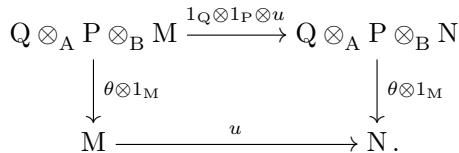
\includegraphics[keepaspectratio]{images/part001_2598f5b2.jpg}}

THEOREM 1. --- Let A and B be k-algebras and P an \((A,B)_{k}\) -bimodule. Denote the \((B,A)_{k}\) -bimodule \(\operatorname{Hom}_{\mathrm{A}}(\mathrm{P},\mathrm{A}_{s})\) by \(P^{*}\) . The following properties are equivalent:

\begin{enumerate}
\def\labelenumi{(\roman{enumi})}
\item
  The \((\mathrm{A},\mathrm{B})_k\) -bimodule P is invertible.
\item
  The A-module P is projective, finitely generated, and generating, and the mapping \(b \mapsto b_{P}\) from B to \(\operatorname{End}_{\mathrm{A}}(\mathrm{P})^{\circ}\) is a k-algebra isomorphism.
\item
  The right B-module P is projective, finitely generated, and generating, and the mapping \(a \mapsto a_{P}\) from A to \(\operatorname{End}_{\mathrm{B}}(\mathrm{P})\) is a k-algebra isomorphism. If these properties hold, then the homomorphisms
\end{enumerate}

\[
\Theta : \mathrm{P} ^ {*} \otimes \mathrm{P} \to {} _ {s} \mathrm{B} _ {d} \quad \text{and} \quad \Lambda : \mathrm{P} \otimes \mathrm{P} ^ {*} \to {} _ {s} \mathrm{A} _ {d}
\]

are isomorphisms, so that the \((\mathrm{B},\mathrm{A})_k\) -bimodule \(\mathrm{P}^*\) is an inverse of \(\mathrm{P}\) .

If property (ii) holds, then P is an invertible \((\mathrm{A},\mathrm{B})_{k}\) -bimodule with inverse \(P^{*}\) (VIII, p.~98, Proposition 2 and p.~98, Proposition 3). This proves that (ii) implies (i) and the last assertion.

Suppose that the \((\mathrm{A},\mathrm{B})_{k}\) -bimodule P is invertible. Then the A-module P is generating (VIII, p.~98, Proposition 3, (iii) \(\Rightarrow\) (i)). It is therefore faithful and balanced (VIII, p.~82, Theorem 2) and, consequently, the mapping \(a \mapsto a_{p}\) from A to \(\operatorname{End}_{\mathrm{B}}(\mathrm{P})\) is bijective.

Let us now prove that the mapping \(b \mapsto b_{\mathrm{P}}\) from B to \(\mathrm{End}_{\mathrm{A}}(\mathrm{P})\) is bijective. Let Q be a \((\mathrm{B},\mathrm{A})_k\) -bimodule, inverse to P. Let \(u \in \mathrm{End}_{\mathrm{A}}(\mathrm{P})\) ; then \(1_{\mathrm{Q}} \otimes u\) is an endomorphism of the left B-module \(\mathbf{Q} \otimes_{\mathrm{A}} \mathbf{P}\) . Since the \((\mathrm{B},\mathrm{B})_k\) -bimodule \(\mathbf{Q} \otimes_{\mathrm{A}} \mathbf{P}\) is isomorphic to \({}_s\mathbf{B}_d\) , there exists a unique element \(b\) of B such that \(1_{\mathrm{Q}} \otimes u\) is the homothety with ratio \(b\) of the right B-module \(\mathbf{Q} \otimes_{\mathrm{A}} \mathbf{P}\) . Consequently, we have \(1_{\mathrm{Q}} \otimes (u - b_{\mathrm{P}}) = 0\) . Hence, \(u = b_{\mathrm{P}}\) by Lemma 1; this proves that the mapping \(b \mapsto b_{\mathrm{P}}\) from B to \(\operatorname{End}_{\mathrm{A}}(\mathrm{P})\) is bijective.

By Proposition 2 of VIII, p.~98, the A-module P is then projective and finitely generated. We have therefore proved the equivalence of (i) and (ii).

By interchanging the roles of A and B, we obtain the equivalence of (i) and (iii), which concludes the proof of the proposition.

COROLLARY 1. --- Let A and B be Morita equivalent k-algebras, and let P be an invertible \((A,B)_{k}\) -bimodule. There exists an isomorphism \(\varphi\) from the center \(Z(A)\) of A to the center of B determined by the relation \(\varphi(z)_{\mathrm{P}} = z_{\mathrm{P}}\) for every \(z \in Z(A)\) . The automorphisms of the \((A,B)_{k}\) -bimodule P are the homotheties \(z_{P}\) where z is an invertible element of \(Z(A)\) .

Given Theorem 1, this follows from Remark 2 of VIII, p.~97.

COROLLARY 2. --- Let A and B be Morita equivalent k-algebras, and let P be an invertible \((\mathrm{A},\mathrm{B})_{k}\) -bimodule. Every \((\mathrm{B},\mathrm{A})_{k}\) -bimodule inverse to P is isomorphic to the dual \(\mathrm{P}^{*}=\mathrm{Hom}_{\mathrm{A}}(\mathrm{P},\mathrm{A})\) of P. More precisely, let Q be a \((\mathrm{B},\mathrm{A})_{k}\) -bimodule that is an inverse of P, and let \(\lambda:P\otimes_{B}Q\to_{s}A_{d}\) be an isomorphism of \((\mathrm{A},\mathrm{A})_{k}\) -bimodules. There exists a unique mapping \(\tau:\mathrm{Q}\to\mathrm{P}^{*}\) determined by the relation \(\langle p,\tau(q)\rangle=\lambda(p\otimes q)\) for \(p\in P\) and \(q\in Q\) , and \(\tau\) is an isomorphism of \((\mathrm{B},\mathrm{A})_{k}\) -bimodules.

The existence and uniqueness of the mapping \(\tau\) are clear. It is a homomorphism of \((\mathrm{B},\mathrm{A})_{k}\) -bimodules, and we have \(\lambda=\Lambda\circ(1_{\mathrm{P}}\otimes\tau)\) . Since \(\lambda\) and \(\Lambda\) are isomorphisms of \((\mathrm{A},\mathrm{A})_{k}\) -bimodules (VIII, p.~101, Theorem 1), so is \(1_{P}\otimes\tau\) . By Lemma 1, the mapping \(\tau\) is bijective.

Remark. --- Under the assumptions of the corollary, let q be an element of Q such that we have \(\lambda(p \otimes q) = 0\) for every \(p \in P\) . We then have \(\tau(q) = 0\) , that is, q = 0. Likewise, if p is an element of P such that we have \(\lambda(p \otimes q) = 0\) for every \(q \in Q\) , then p = 0.

Examples. --- 1) Let B be a \(k\) -algebra, \(n\) an integer \(\geqslant 1\) , and A the \(k\) -algebra \(\mathbf{M}_n(\mathrm{B})\) . The right B-module \(\mathrm{P} = \mathrm{B}_d^n\) is projective, finitely generated, and generating, and A can be identified with the endomorphism algebra of P (II, §10, No.~7, p.~349). By Theorem 1, the \((\mathrm{A},\mathrm{B})_k\) -bimodule P is invertible. The algebras B and \(\mathbf{M}_n(\mathrm{B})\) are therefore Morita equivalent.

\begin{enumerate}
\def\labelenumi{\arabic{enumi})}
\setcounter{enumi}{1}
\tightlist
\item
  *Let A be a commutative \(k\) -algebra and P an A-module. We view P as an \((A, A)_k\) -bimodule whose two laws of action are equal. If the \((A, A)_k\) -bimodule P is invertible, then the A-module P is finitely generated (Theorem 1). By Theorem 3 of Comm. Alg., II, §5, No.~4, p.~114, the following properties are equivalent:
\end{enumerate}

\begin{enumerate}
\def\labelenumi{(\roman{enumi})}
\item
  The \((\mathrm{A},\mathrm{A})_{k}\) -bimodule P is invertible.
\item
  There exists an A-module \(\mathrm{Q}\) such that \(\mathrm{P} \otimes_{\mathrm{A}} \mathrm{Q}\) is isomorphic to \(\mathrm{A}\) .
\item
  The A-module P is projective, finitely generated, and of rank 1. *
\end{enumerate}

\subsection{The Morita Correspondence of Modules}

In this subsection, the letters A and B denote Morita equivalent k-algebras and P an invertible \((A,B)_{k}\) -bimodule. Choose a \((B,A)_{k}\) -bimodule Q inverse to P and isomorphisms

\[
\lambda : \mathrm{P} \otimes_ {\mathrm{B}} \mathrm{Q} \rightarrow {} _ {s} \mathrm{A} _ {d} \quad \text { and } \quad \theta : \mathrm{Q} \otimes_ {\mathrm{A}} \mathrm{P} \rightarrow {} _ {s} \mathrm{B} _ {d}.
\]

For any left B-module V, denote by \(\theta_{V}\) the homomorphism of B-modules \(\theta\otimes1_{V}:Q\otimes_{A}P\otimes_{B}V\to V\) ; it is an isomorphism since \(\theta\) is an isomorphism. Likewise, for every left A-module M, denote by \(\lambda_{M}\) the homomorphism of A-modules \(\lambda\otimes1_{M}:P\otimes_{B}Q\otimes_{A}M\to M\) ; it is an isomorphism since \(\lambda\) is an isomorphism.

THEOREM 2 (Morita). --- a) Let V and W be left B-modules. The mapping \(g \mapsto 1_{\mathrm{P}} \otimes g\) is a bijection from \(\operatorname{Hom}_{\mathrm{B}}(\mathrm{V}, \mathrm{W})\) to \(\operatorname{Hom}_{\mathrm{A}}(\mathrm{P} \otimes_{\mathrm{B}} \mathrm{V}, \mathrm{P} \otimes_{\mathrm{B}} \mathrm{W})\) . The inverse bijection sends an element h of \(\operatorname{Hom}_{\mathrm{A}}(\mathrm{P} \otimes_{\mathrm{B}} \mathrm{V}, \mathrm{P} \otimes_{\mathrm{B}} \mathrm{W})\) to the element \(\theta_{\mathrm{W}} \circ (1_{\mathrm{Q}} \otimes h) \circ \theta_{\mathrm{V}}^{-1}\) of \(\operatorname{Hom}_{\mathrm{B}}(\mathrm{V}, \mathrm{W})\) .

\begin{enumerate}
\def\labelenumi{\alph{enumi})}
\setcounter{enumi}{1}
\tightlist
\item
  Every left A-module M is isomorphic to a module of the form \(\mathrm{P} \otimes_{\mathrm{B}} \mathrm{V}\) , where V is a left B-module.
\end{enumerate}

Let V and W be left B-modules. By Lemma 1 of VIII, p.~101, the mapping \(\varphi : g \mapsto 1_{\mathrm{P}} \otimes g\) from \(\mathrm{Hom}_{\mathrm{B}}(\mathrm{V}, \mathrm{W})\) to \(\mathrm{Hom}_{\mathrm{A}}(\mathrm{P} \otimes_{\mathrm{B}} \mathrm{V}, \mathrm{P} \otimes_{\mathrm{B}} \mathrm{W})\) is injective. By interchanging the roles of P and Q (and of A and B), we see that the mapping \(\psi : h \mapsto 1_{\mathrm{Q}} \otimes h\) from \(\mathrm{Hom}_{\mathrm{A}}(\mathrm{P} \otimes_{\mathrm{B}} \mathrm{V}, \mathrm{P} \otimes_{\mathrm{B}} \mathrm{W})\) to \(\mathrm{Hom}_{\mathrm{A}}(\mathrm{Q} \otimes_{\mathrm{A}} \mathrm{P} \otimes_{\mathrm{B}} \mathrm{V}, \mathrm{Q} \otimes_{\mathrm{A}} \mathrm{P} \otimes_{\mathrm{B}} \mathrm{W})\) is also injective. Now, the composition \(\psi \circ \varphi\) is the mapping \(g \mapsto \theta_{\mathrm{W}}^{-1} \circ g \circ \theta_{\mathrm{V}}\) . It is bijective, hence so is \(\psi\) . Consequently, \(\varphi\) is bijective, and its inverse is the mapping \(h \mapsto \theta_{\mathrm{W}} \circ (1_{\mathrm{Q}} \otimes h) \circ \theta_{\mathrm{V}}^{-1}\) .

Assertion b) follows from the fact that \(\lambda_{\mathrm{M}}\) is an isomorphism from \(\mathrm{P} \otimes_{\mathrm{B}} \otimes_{\mathrm{A}} \otimes_{\mathrm{M}}\) to \(\mathrm{M}\) .

Let V be a left B-module and W a submodule of V. Since the B-module P is projective (VIII, p.~101, Theorem 1), the canonical mapping from \(P \otimes_{B} W\) to \(P \otimes_{B} V\) is injective. We identify \(P \otimes_{B} W\) with its image in \(P \otimes_{B} V\) through this mapping. We adopt the analogous conventions when P and B are replaced by Q and A.

PROPOSITION 5. --- Let V be a left B-module. The mapping \(W \mapsto P \otimes_{B} W\) is an isomorphism from the set of B-submodules of V, ordered by inclusion, to the set of A-submodules of \(P \otimes_{B} V\) , ordered by inclusion. The inverse isomorphism sends an A-submodule N of \(P \otimes_{B} V\) to the image under \(\theta_{V}\) of the B-submodule \(Q \otimes_{A} N\) of \(Q \otimes_{A} P \otimes_{B} V\) .

Denote by \(D_{\mathrm{B}}(\mathrm{V})\) the set of B-submodules of V, ordered by inclusion, and define the sets \(D_{\mathrm{A}}(\mathrm{P}\otimes_{\mathrm{B}}\mathrm{V})\) and \(D_{\mathrm{B}}(\mathrm{Q}\otimes_{\mathrm{A}}\mathrm{P}\otimes_{\mathrm{B}}\mathrm{V})\) likewise. Let \(\varphi:D_{\mathrm{B}}(\mathrm{V})\to D_{\mathrm{A}}(\mathrm{P}\otimes_{\mathrm{B}}\mathrm{V})\) be the mapping \(W\mapsto P\otimes_{B}W\) and \(\psi\) the mapping from \(D_{\mathrm{A}}(\mathrm{P}\otimes_{\mathrm{B}}\mathrm{V})\) to \(D_{\mathrm{B}}(\mathrm{Q}\otimes_{\mathrm{A}}\mathrm{P}\otimes_{\mathrm{B}}\mathrm{V})\) given by \(N\mapsto Q\otimes_{A}N\) . These are increasing mappings, and the composition \(\psi\circ\varphi\) is the mapping \(W\mapsto\theta_{\mathrm{V}}^{-1}(\mathrm{W})\) , which is bijective. Consequently, \(\varphi\) is injective, and \(\psi\) is surjective. By replacing B with A and V with \(P\otimes_{B}V\) , we see that \(\psi\) is also injective. Hence, \(\varphi\) and \(\psi\) are bijective, and the inverse mapping of \(\varphi\) is indeed that described in the proposition.

Examples. --- 1) Let us apply Proposition 5 of VIII, p.~104, to the specific case \(\mathrm{V} = \mathrm{B}_s\) .

\begin{enumerate}
\def\labelenumi{\alph{enumi})}
\item
  The mapping \(J \mapsto PJ\) is an isomorphism from the ordered set \(\mathrm{D}(\mathrm{B}_{s})\) of left ideals of B to the ordered set \(\mathrm{D}(\mathrm{P})\) of A-submodules of P. The inverse mapping sends an A-submodule M of P to the left ideal \(\mathrm{J}(\mathrm{M})\) of B consisting of the elements b of B such that M contains Pb.
\item
  The mapping \(K \mapsto KP\) is an isomorphism from the ordered set \(\mathrm{D}(A_{d})\) of right ideals of A to the ordered set \(\mathrm{D}(P)\) of B-submodules of P. The inverse mapping sends a B-submodule V of P to the right ideal \(\mathrm{K}(V)\) of A consisting of the elements a of A such that V contains aP.
\end{enumerate}

Indeed, the A-module \(P \otimes_{B} B_{s}\) can be canonically identified with P. If J is a left ideal of B, then the canonical image of \(P \otimes_{B} J\) in \(P \otimes_{B} B_{s}\) corresponds to PJ through this identification. Consequently, the mapping \(J \mapsto PJ\) is an isomorphism of ordered sets from \(D(B_{s})\) to \(D(P)\) . Let \(J \in D(B_{s})\) . Denote the set of elements b of B such that PJ contains Pb by \(J'\) . It is a left ideal of B that contains J, and we have \(PJ' \subset PJ\) . Since the mapping \(J \mapsto PJ\) is an isomorphism of ordered sets, we necessarily have \(PJ' = PJ\) and \(J = J'\) . This proves a).

Assertion b) follows from assertion a) applied to the invertible \((\mathrm{B}^{\circ},\mathrm{A}^{\circ})_{k}\) -bimodule P.

Note that the ring A is a field if and only if the B-module P is simple.

\begin{enumerate}
\def\labelenumi{\arabic{enumi})}
\setcounter{enumi}{1}
\tightlist
\item
  Denote by \(\mathcal{B}_{\mathrm{A}}\) , \(\mathcal{B}_{\mathrm{B}}\) , and \(\mathcal{B}_{\mathrm{P}}\) the sets of two-sided ideals of A, two-sided ideals of B, and \((\mathrm{A},\mathrm{B})_k\) -sub-bimodules of P, respectively.
\end{enumerate}

\begin{enumerate}
\def\labelenumi{\alph{enumi})}
\item
  The mapping \(\mathfrak{b} \mapsto \mathrm{P}\mathfrak{b}\) is an isomorphism of ordered sets from \(\mathcal{B}_{\mathrm{B}}\) to \(\mathcal{B}_{\mathrm{P}}\) ; the inverse isomorphism sends an \((\mathrm{A},\mathrm{B})_k\) -sub-bimodule \(\mathrm{P}'\) of \(\mathrm{P}\) to the two-sided ideal of \(\mathrm{B}\) consisting of the elements \(b\) such that \(\mathrm{P}b \subset \mathrm{P}'\) .
\item
  The mapping \(a \mapsto aP\) is an isomorphism of ordered sets from \(B_{A}\) to \(B_{P}\) ; the inverse isomorphism sends an \((A, B)_{k}\) -sub-bimodule \(P'\) of P to the two-sided ideal of A consisting of the elements a such that \(aP \subset P'\) .
\end{enumerate}

Indeed, let J be a left ideal of B and \(P' = PJ\) . Then \(P'\) is an A-submodule of P and, by Example 1, the ideal J consists of the elements b of B such that \(Pb \subset P'\) . Moreover, \(P'\) is an \((A, B)_{k}\) -sub-bimodule of P if and only if J is a two-sided ideal of B. Thus a) follows from loc. cit.

Assertion b) follows from assertion a) applied to the invertible \((\mathrm{B}^{\circ}, \mathrm{A}^{\circ})_{k}\) -bimodule P.

PROPOSITION 6. --- Denote by \(\mathcal{B}_{\mathrm{A}}\) and \(\mathcal{B}_{\mathrm{B}}\) the sets of two-sided ideals of A and two-sided ideals of B.

\begin{enumerate}
\def\labelenumi{\alph{enumi})}
\item
  There exists an isomorphism of ordered sets \(f\) from \(\mathcal{B}_{\mathrm{A}}\) to \(\mathcal{B}_{\mathrm{B}}\) determined by the following property: if \(\mathfrak{a}\) is a two-sided ideal of \(\mathrm{A}\) and \(\mathfrak{b}\) a two-sided ideal of \(\mathrm{B}\) , then the relation \(f(\mathfrak{a}) = \mathfrak{b}\) is equivalent to \(\mathfrak{a}\mathrm{P} = \mathrm{P}\mathfrak{b}\) .
\item
  Suppose that the ring A is commutative, so that A can be identified with the center of B (VIII, p.~102, Corollary 1). The isomorphism \(f: \mathcal{B}_{\mathrm{A}} \to \mathcal{B}_{\mathrm{B}}\) sends an ideal \(\mathfrak{a}\) of A to the two-sided ideal \(\mathrm{Ba}\) of B, and we have \(\mathfrak{a} = \mathrm{A} \cap \mathrm{Ba}\) .
\end{enumerate}

Assertion a) follows from Example 2.

Now, suppose that A is commutative, and identify A with the center of B. Let a be an ideal of A. Then Ba is a two-sided ideal of B; we have PBa = aP and therefore \(f(a) = \text{Ba}\) . Let \(a'\) be the ideal \(A \cap Ba\) of A; it is contained in Ba and contains a, so \(Ba'\) is equal to Ba. Since f is bijective, it follows that \(a' = a\) .

Examples. --- 3) Let V be a left B-module. Then the correspondence given above sends the annihilator of the B-module V to the annihilator of the A-module \(P \otimes_{B} V\) . Indeed, denote the annihilator of the A-module \(P \otimes_{B} V\) by a and that of the B-module V by b. Let W be the \((A, B)_{k}\) -sub-bimodule of P consisting of the elements such that \(p \otimes v = 0\) for every element v of V. We have the inclusion \(Pb \subset W\) ; conversely, for every \(p \in W\) and \(q \in Q\) , we have that \(\theta(q \otimes p)\) belongs to b. Hence, the element b of \(D(B_s)\) corresponds to the element W of D(P). Likewise, \(a \in D(A_d)\) corresponds to W.

\begin{enumerate}
\def\labelenumi{\arabic{enumi})}
\setcounter{enumi}{3}
\tightlist
\item
  For any two-sided ideal \(\mathfrak{a}\) of A, denote the subset of \(\mathbf{M}_n(\mathrm{A})\) consisting of the matrices with entries in \(\mathfrak{a}\) by \(\mathbf{M}_n(\mathfrak{a})\) . It is a two-sided ideal of \(\mathbf{M}_n(\mathrm{A})\) . We have \(\mathbf{M}_n(\mathfrak{a})\mathrm{A}^n = \mathfrak{a}^n = \mathrm{A}^n\mathfrak{a}\) . It follows from Proposition 6 that every two-sided ideal of \(\mathbf{M}_n(\mathrm{A})\) is of the form \(\mathbf{M}_n(\mathfrak{a})\) , where \(\mathfrak{a}\) is a two-sided ideal of A.
\end{enumerate}

Remark. --- We keep the assumptions and notation above and suppose that the \((\mathrm{B},\mathrm{A})_{k}\) -bimodule Q is the dual \(P^{*}\) of the A-module P and that the isomorphisms \(\lambda\) and \(\theta\) are the canonical mappings \(\Lambda:P\otimes_{B}P^{*}\to_{s}A_{d}\) and \(\Theta:P^{*}\otimes_{A}P\to_{s}B_{d}\) (VIII, p.~101, Theorem 1). Since the A-module P is projective and finitely generated, we have a canonical isomorphism \(\vartheta_{M}:P^{*}\otimes_{A}M\to\operatorname{Hom}_{A}(P,M)\) for every A-module M (II, §4, No.~2, p.~271, Corollary). We leave it to the reader to reformulate the results of Subsections 3 and 4 by replacing the construction \(M\mapsto Q\otimes_{A}M\) with the construction \(M\mapsto\operatorname{Hom}_{A}(P,M)\) .

\subsection{Ordered Sets of Submodules}

In this subsection, A and B are k-algebras, M is a left A-module, and V is a left B-module. We denote by \(\mathrm{D}(\mathrm{M})\) (resp. \(\mathrm{D}(\mathrm{V})\) ) the set of submodules of M (resp. of V), ordered by inclusion. We assume given an isomorphism of ordered sets \(\varphi : \mathrm{D}(\mathrm{V}) \to \mathrm{D}(\mathrm{M})\) .

By Morita's theorem (VIII, p.~103, Theorem 2), we obtain such an isomorphism in the following situation: P is an invertible \((\mathrm{A},\mathrm{B})_k\) -bimodule, M is the A-module \(\mathrm{P} \otimes_{\mathrm{B}} \mathrm{V}\) , and for every submodule W of V, \(\varphi(\mathrm{W})\) is the canonical image of \(\mathrm{P} \otimes_{\mathrm{B}} \mathrm{W}\) in M.

Some properties of the module M, or of its submodules, can be expressed in terms of the ordered set D(M): they are listed in Tables I and II.

The module M is the direct sum of a family \((\mathrm{M}_{i})_{i\in\mathrm{I}}\) of submodules if and only if we have \(M=\sum_{i\in I}M_{i}\) and \(M_{i}\cap\sum_{j\neq i}M_{j}=0\) for every \(i\in I\) . This remark and an examination of Table I give the following result.

PROPOSITION 7. --- a) We have \(\varphi(0)=0\) and \(\varphi(V)=M\) .

\begin{enumerate}
\def\labelenumi{\alph{enumi})}
\setcounter{enumi}{1}
\tightlist
\item
  Let \((\mathrm{V}_i)_{i\in \mathrm{I}}\) be a family of submodules of V. We have
\end{enumerate}

\[
\varphi \left(\sum_ {i \in \mathrm{I}} \mathrm{V} _ {i}\right) = \sum_ {i \in \mathrm{I}} \varphi (\mathrm{V} _ {i}), \quad \varphi \left(\bigcap_ {i \in \mathrm{I}} \mathrm{V} _ {i}\right) = \bigcap_ {i \in \mathrm{I}} \varphi (\mathrm{V} _ {i}).
\]

Submodules of M

Ordered set D(M)

Zero submodule

Smallest element of D(M)

Submodule M

Greatest element of D(M)

\(\bigcap_{i\in I} M_i\)

Greatest lower bound \(\inf_{i\in I} M_i\)

\(\sum_{i\in I} M_i\)

Least upper bound \(\sup_{i\in I} M_i\)

Supplementary submodules

\(\inf(M', M'') = 0, \sup(M', M'') = M\)

Simple submodule of M

Minimal element of D(M) --- \{0\}

Maximal submodule of M

Maximal element of D(M) --- \{M\}

Socle \(\mathscr{S}(M)\) of M

Least upper bound in D(M) of the set of minimal elements of D(M) --- \{0\}

\emph{Radical \(\Re(M)\) of M}(VIII, p.~151)

Greatest lower bound in D(M) of the set of maximal elements of D(M) --- \{M\}

Properties of the module M

Properties of D(M)

M is Noetherian.

The ordered set D(M) is Noetherian (Set Theory, III, §6, No.~5, p.~190).

M is Artinian.

The set D(M), ordered by ⊃, is Noetherian.

M is indecomposable.

We have M ≠ 0, and there are no two nonzero elements M\textquotesingle{} and M\textquotesingle\textquotesingle{} of D(M) satisfying inf(M\textquotesingle, M\textquotesingle\textquotesingle) = 0, sup(M\textquotesingle, M\textquotesingle\textquotesingle) = M.

M is finitely generated.

For every family (Mi) i∈I in D(M) with upper bound M, there exists a finite subset J of I such that M = supj∈I Mj.

M is simple.

Card(D(M)) = 2.

M is semisimple.

M is the least upper bound, in D(M), of the set of minimal elements of D(M) = \{0\}.

TABLE II.

\begin{enumerate}
\def\labelenumi{\alph{enumi})}
\setcounter{enumi}{2}
\tightlist
\item
  The B-module V is the direct sum of the family \((\mathrm{V}_{i})_{i\in\mathrm{I}}\) of submodules if and only if M is the direct sum of the family \((\varphi(\mathrm{V}_{i}))_{i\in\mathrm{I}}\) .
\end{enumerate}

Let \(V'\) and \(V''\) be submodules of \(V\) such that \(V'\) is contained in \(V''\) ; set \(M' = \varphi(V')\) and \(M'' = \varphi(V'')\) , so that \(M''\) contains \(M'\) . Denote by \([V', V'']\) the interval in \(D(V)\) consisting of the submodules \(W\) of \(V\) such that we have \(V' \subset W \subset V''\) , and define the interval \([M', M'']\) in \(D(M)\) likewise. The mapping \(W \mapsto W/V'\) is an isomorphism of ordered sets from \([V', V'']\) to \(D(V''/V')\) ; we define an isomorphism of ordered sets from \([M', M'']\) to \(D(M''/M')\) likewise. Since \(\varphi\) sends the interval \([V', V'']\) to \([M', M'']\) , it defines an isomorphism \(\varphi\) of ordered sets from \(D(V''/V')\) to \(D(M''/M')\) . We deduce the following proposition from this and Tables I and II.

PROPOSITION 8. --- a) Let V' and V'\,' be submodules of V such that V'\,' contains V'. The B-module V'\,'/V' is simple if and only if the A-module \(\varphi(\mathrm{V}^{\prime\prime})/\varphi(\mathrm{V}^{\prime})\) is simple.

\begin{enumerate}
\def\labelenumi{\alph{enumi})}
\setcounter{enumi}{1}
\item
  If \(V'\) is a simple submodule, maximal submodule, or direct factor of V, then \(\varphi(V')\) is, respectively, a simple submodule, maximal submodule, or direct factor of M.
\item
  The isomorphism \(\varphi\) transforms the socle \(\mathcal{S}(\mathrm{V})\) of \(\mathrm{V}\) into the socle \(\mathcal{S}(\mathrm{M})\) of \(\mathrm{M}^*\) and the radical (VIII, p.~151, Definition 1) \(\Re (\mathrm{V})\) of \(\mathrm{V}\) into the radical \(\Re (\mathrm{M})\) of \(\mathrm{M}_{*}\)
\item
  Let \((\mathrm{V}_{i})_{0\leqslant i\leqslant n}\) be a finite sequence of submodules of V. It is a Jordan-Hölder series of V if and only if \((\varphi(\mathrm{V}_{i})_{0\leqslant i\leqslant n})\) is a Jordan-Hölder series of M.
\end{enumerate}

Lemma 2. --- Let H and H' be submodules of V such that \(H \cap H' = 0\) . The B-modules H and H' are isomorphic if and only if the A-modules \(\varphi(\mathrm{H})\) and \(\varphi(\mathrm{H}')\) are isomorphic.

We identify \(H+H'\) with the product \(H \times H'\) . The graph of an isomorphism from H to \(H'\) is a submodule \(H''\) of V satisfying

\[
\mathrm{H} \cap \mathrm{H} ^ {\prime \prime} = \mathrm{H} ^ {\prime} \cap \mathrm{H} ^ {\prime \prime} = 0, \quad \mathrm{H} + \mathrm{H} ^ {\prime} = \mathrm{H} + \mathrm{H} ^ {\prime \prime} = \mathrm{H} ^ {\prime} + \mathrm{H} ^ {\prime \prime};\tag{17}
\]

conversely, every submodule that has these properties is the graph of an isomorphism from H to \(H'\) . By Proposition 7, the relation \(H \cap H' = 0\) is equivalent to \(\varphi(\mathrm{H}) \cap \varphi(\mathrm{H}') = 0\) , and relations (17) are equivalent to the relations

\[
\varphi (\mathrm{H}) \cap \varphi (\mathrm{H} ^ {\prime \prime}) = \varphi (\mathrm{H} ^ {\prime}) \cap \varphi (\mathrm{H} ^ {\prime \prime}) = 0,
\]

\[
\varphi (\mathrm{H}) + \varphi (\mathrm{H} ^ {\prime}) = \varphi (\mathrm{H}) + \varphi (\mathrm{H} ^ {\prime \prime}) = \varphi (\mathrm{H} ^ {\prime}) + \varphi (\mathrm{H} ^ {\prime \prime});
\]

the lemma follows.

PROPOSITION 9. --- Let S be a simple submodule of V and T the simple submodule \(\varphi(\mathrm{S})\) of M. If \(V_{S}\) denotes the isotypical component of V of type S and \(M_{T}\) the isotypical component of M of type T, then we have \(\varphi(V_{\mathrm{S}})=M_{\mathrm{T}}\) .

Every simple submodule \(S'\) of V distinct from S satisfies \(S' \cap S = 0\) . It is therefore isomorphic to S if and only if \(\varphi(S')\) is isomorphic to T (Lemma 2). Now, \(V_{S}\) is the sum of the simple submodules of V isomorphic to S, and \(M_{T}\) is the sum of the simple submodules of M isomorphic to T. Proposition 9 therefore follows immediately from Propositions 7 and 8.

PROPOSITION 10. --- a) The B-module V is Artinian (resp. Noetherian, indecomposable, simple, finitely generated) if and only if M is.

\begin{enumerate}
\def\labelenumi{\alph{enumi})}
\setcounter{enumi}{1}
\item
  The B-module V has finite length if and only if the A-module M has finite length, and we then have \(\mathrm{long}_{\mathrm{B}}(\mathrm{V}) = \mathrm{long}_{\mathrm{A}}(\mathrm{M})\) .
\item
  The B-module V is semisimple (resp. isotypical) if and only if the A-module M is semisimple (resp. isotypical). If this is the case, then we have \(\text{long}_{\text{B}}(\text{V}) = \text{long}_{\text{A}}(\text{M})\) .
\end{enumerate}

Assertion a) follows from the second property listed in Table II.

Assertion b) follows from Proposition 8, d).

The module V is semisimple if and only if it is equal to its socle \(\mathcal{S}(V)\) ; it is isotypical if and only if there exists a simple submodule S of V such that \(V = V_{S}\) . Assertion c) therefore follows from Propositions 7, c), 8, c), and 9 (VIII, p.~106 and 109).

\subsection{Other Properties Preserved by the Morita Correspondence}

Let A and B be Morita equivalent k-algebras and P an invertible \((A,B)_{k}\) -bimodule.

PROPOSITION 11. --- Let

\[
\mathrm{V} ^ {\prime} \xrightarrow {f} \mathrm{V} \xrightarrow {g} \mathrm{V} ^ {\prime \prime}\tag{ε}
\]

be a diagram of B-modules and B-linear mappings, and let

\[
(\mathrm{P} \otimes \mathcal {E})
\]

\[
\mathrm{P} \otimes_ {\mathrm{B}} \mathrm{V} ^ {\prime} \xrightarrow {1 _ {\mathrm{P}} \otimes f} \mathrm{P} \otimes_ {\mathrm{B}} \mathrm{V} \xrightarrow {1 _ {\mathrm{P}} \otimes g} \mathrm{P} \otimes_ {\mathrm{B}} \mathrm{V} ^ {\prime \prime}
\]

be the corresponding diagram of A-modules. Then \((\mathcal{E})\) is an exact sequence if and only if \((\mathrm{P} \otimes \mathcal{E})\) is an exact sequence.

Suppose that the sequence \((\mathcal{E})\) is exact. Since the right B-module P is projective, the sequence \((P \otimes \mathcal{E})\) is exact (II, §3, No.~6, p.~251, Proposition 5 and II, §3, No.~7, p.~257, Corollary 6).

Conversely, suppose that the sequence \((\mathrm{P} \otimes \mathcal{E})\) is exact. Let Q be a \((\mathrm{B}, \mathrm{A})_{k}\) -bimodule, inverse to P, and \(\theta : Q \otimes_{A} P \to {}_{s} B_{d}\) an isomorphism. Consider the commutative diagram

\[
\begin{array}{c} \mathrm{Q} \otimes_ {\mathrm{A}} \mathrm{P} \otimes_ {\mathrm{B}} \mathrm{V} ^ {\prime} \xrightarrow {1 _ {\mathrm{Q}} \otimes 1 _ {\mathrm{P}} \otimes f} \mathrm{Q} \otimes_ {\mathrm{A}} \mathrm{P} \otimes_ {\mathrm{B}} \mathrm{V} \xrightarrow {1 _ {\mathrm{Q}} \otimes 1 _ {\mathrm{P}} \otimes g} \mathrm{Q} \otimes_ {\mathrm{A}} \mathrm{P} \otimes_ {\mathrm{B}} \mathrm{V} ^ {\prime \prime} \\ \theta \otimes 1 _ {\mathrm{V} ^ {\prime}} \Biggl \downarrow \\ \mathrm{V} ^ {\prime} \xrightarrow {f} \mathrm{V} \xrightarrow {g} \mathrm{V} ^ {\prime \prime}. \end{array}
\]

Since Q is a projective A-module and the sequence \((\mathrm{P} \otimes \mathcal{E})\) is exact, the first line of this diagram is an exact sequence. Since the vertical arrows are isomorphisms, the second line is also exact.

COROLLARY. --- Let \(f: V \rightarrow W\) be a B-linear mapping. Then f is injective (resp. surjective) if and only if \(1_{P} \otimes f\) is.

PROPOSITION 12. --- Let V be a left B-module. The B-module V is projective (resp. generating, faithful, *injective, finitely presented*) if and only if the A-module P ⊗\_B V is.

\begin{enumerate}
\def\labelenumi{\alph{enumi})}
\item
  Suppose that V is projective. There exists a set I such that V is isomorphic to a direct factor submodule of \(\mathrm{B}_{s}^{(\mathrm{I})}\) . The A-module \(P \otimes_{B} V\) is then isomorphic to a direct factor submodule of \(\mathrm{P}^{(\mathrm{I})}\) ; since P is a projective A-module, the same holds for \(P \otimes_{B} V\) .
\item
  Suppose that the B-module V is generating. Let M be an A-module. There exists a B-module W such that M is isomorphic to \(P \otimes_{B} W\) . By Theorem 1 of VIII, p.~80, there exist a set I and a surjection \(\varphi : V^{(I)} \to W\) . By the corollary, the mapping \(1_{P} \otimes \varphi\) from \(P \otimes (V^{(I)})\) to \(P \otimes_{A} W\) is surjective, which gives a surjection \((P \otimes V)^{(I)} \to M\) . By Theorem 1 of VIII, p.~80, \(P \otimes V\) is a generating A-module.
\item
  The B-module V is faithful if and only if its annihilator is reduced to 0. Assertion c) therefore follows from Example 3 of VIII, p.~105.
\end{enumerate}

*d) Suppose that V is injective. By the remark of VIII, p.~106, the A-module \(\mathrm{P} \otimes_{\mathrm{B}} \mathrm{V}\) is isomorphic to \(\mathrm{Hom}_{\mathrm{B}}(\mathrm{Q}, \mathrm{V})\) , where Q is a \((\mathrm{B}, \mathrm{A})_k\) -bimodule inverse to A. Since the A-module Q is projective, hence flat (X, §1, n° 3, p.~9, example 1), the A-module \(\mathrm{Hom}_{\mathrm{B}}(\mathrm{Q}, \mathrm{V})\) is injective by X, §1, n° 8, p.~18, proposition 11.

\begin{enumerate}
\def\labelenumi{\alph{enumi})}
\setcounter{enumi}{4}
\item
  Suppose that V admits a finite presentation \(L_{1} \to L_{0} \to V \to 0\) (X, §1, n° 4, p.~10). By taking the tensor product with P, we deduce an exact sequence of A-modules \(N_{1}^{\prime} \xrightarrow{u} N_{0}^{\prime} \to P \otimes_{B} V \to 0\) , where \(N_{1}^{\prime}\) and \(N_{0}^{\prime}\) are projective and finitely generated (Proposition 11 and a)). Let \(N_{0}^{\prime\prime}\) be a finitely generated A-module such that the module \(N_{0} = N_{0}^{\prime} \oplus N_{0}^{\prime\prime}\) is free and finitely generated, and let \(u^{\prime}: N_{1}^{\prime} \oplus N_{0}^{\prime\prime} \to N_{0}\) be the homomorphism \((u, 1_{N_{0}^{\prime\prime}})\) ; then \(P \otimes_{B} V\) can be identified with the cokernel of \(u^{\prime}\) . Let \(N_{1}\) be a finitely generated free A-module and \(p: N_{1} \to N_{1}^{\prime} \oplus N_{0}^{\prime\prime}\) a surjective homomorphism; the sequence \(N_{1} \xrightarrow{u^{\prime} \circ p} N_{0} \to P \otimes_{B} V \to 0\) is a finite presentation of the A-module \(P \otimes_{B} V_*\)
\item
  Suppose that the A-module \(P \otimes_{B} V\) is projective (resp. generating, faithful, *injective, finitely presented*). By applying the above (interchanging the roles of A and B and of P and Q), we see that the B-module \(Q \otimes_{A} P \otimes_{B} V\) also has this property. The same is therefore true for the B-module V, which is isomorphic to it.
\end{enumerate}

COROLLARY. --- The ring A is left Artinian (resp. left Noetherian) if and only if the ring B is.

Because of the isomorphism between the ordered set of left ideals of B and the set of A-submodules of P, the ring B is left Artinian (resp. left Noetherian) if and only if the A-module P is Artinian (resp. Noetherian). However, by Theorem 1 of VIII, p.~101, the A-module P is generating and finitely generated; in particular, \(A_{s}\) is isomorphic to a direct factor of \(P^{n}\) for an integer \(n \geqslant 1\) . Consequently, P is Artinian (resp. Noetherian) if and only if A is left Artinian (resp. left Noetherian).

\subsection{Morita Equivalence of Algebras}

PROPOSITION 13. --- a) If two k-algebras are Morita equivalent, then their centers are isomorphic k-algebras.

\begin{enumerate}
\def\labelenumi{\alph{enumi})}
\setcounter{enumi}{1}
\item
  Two commutative \(k\) -algebras are Morita equivalent if and only if they are isomorphic.
\item
  Two k-algebras that are fields are Morita equivalent if and only if they are isomorphic.
\item
  For \(i = 1,2\) , let \(\mathrm{A}_i\) and \(\mathrm{B}_i\) be Morita equivalent \(k\) -algebras and \(\mathrm{P}_i\) an invertible \((\mathrm{A}_i,\mathrm{B}_i)_k\) -bimodule. Set \(\mathrm{A} = \mathrm{A}_1\otimes_k\mathrm{A}_2\) , \(\mathrm{B} = \mathrm{B}_1\otimes_k\mathrm{B}_2\) , and \(\mathrm{P} = \mathrm{P}_1 \otimes_k \mathrm{P}_2\) . The \(k\) -algebras A and B are Morita equivalent, and P is an invertible \((\mathrm{A}, \mathrm{B})_k\) -bimodule.
\item
  If A and B are Morita equivalent \(k\) -algebras and \(k'\) is a commutative \(k\) -algebra, then the \(k'\) -algebras \(\mathrm{A}_{(k')}\) and \(\mathrm{B}_{(k')}\) are Morita equivalent.
\end{enumerate}

Assertion a) follows from Corollary 1 of VIII, p.~102, and implies b).

Let \(\mathrm{K}\) and \(\mathrm{L}\) be \(k\) -algebras that are fields, and let \(\mathrm{P}\) be an invertible \((\mathrm{K},\mathrm{L})_k\) -bimodule. The right \(\mathrm{L}\) -vector space \(\mathrm{P}\) is a simple module (VIII, p.~104), hence of dimension 1, so the \(k\) -algebras \(\operatorname{End}_{\mathrm{L}}(\mathrm{P})\) and \(\mathrm{L}\) are isomorphic. By VIII, p.~101, Theorem 1, the mapping \(a\mapsto a_{\mathrm{P}}\) from \(\mathrm{K}\) to \(\operatorname{End}_{\mathrm{L}}(\mathrm{P})\) is an isomorphism. Therefore, the fields \(\mathrm{K}\) and \(\mathrm{L}\) are isomorphic over \(k\) ; assertion c) follows.

Under the assumptions of d), let \(Q_{i}\) (i = 1, 2) be a \((\mathrm{B}_{i}, \mathrm{A}_{i})_{k}\) -bimodule inverse to \(P_{i}\) . Denote the \((\mathrm{B}, \mathrm{A})_{k}\) -bimodule \(Q_{1} \otimes_{k} Q_{2}\) by Q. Consider the canonical k-linear isomorphism \((\mathrm{P}_{1} \otimes_{k} \mathrm{P}_{2}) \otimes_{k} (\mathrm{Q}_{1} \otimes_{k} \mathrm{Q}_{2}) \to (\mathrm{P}_{1} \otimes_{k} \mathrm{Q}_{1}) \otimes_{k} (\mathrm{P}_{2} \otimes_{k} \mathrm{Q}_{2})\) ; when passing to the quotient, it defines a morphism

\[
\left(\mathrm{P} _ {1} \otimes_ {k} \mathrm{P} _ {2}\right) \otimes_ {\mathrm{B}} \left(\mathrm{Q} _ {1} \otimes_ {k} \mathrm{Q} _ {2}\right)\rightarrow \left(\mathrm{P} _ {1} \otimes_ {\mathrm{B} _ {1}} \mathrm{Q} _ {1}\right) \otimes_ {k} \left(\mathrm{P} _ {2} \otimes_ {\mathrm{B} _ {2}} \mathrm{Q} _ {2}\right)
\]

that is (A,A)-linear. Conversely, the inverse isomorphism \((\mathrm{P}_{1}\otimes_{k}\mathrm{Q}_{1})\otimes_{k}(\mathrm{P}_{2}\otimes_{k}\mathrm{Q}_{2})\to(\mathrm{P}_{1}\otimes_{k}\mathrm{P}_{2})\otimes_{k}(\mathrm{Q}_{1}\otimes_{k}\mathrm{Q}_{2})\) defines an (A,A)-linear morphism \((\mathrm{P}_{1}\otimes_{\mathrm{B}_{1}}\mathrm{Q}_{1})\otimes_{k}(\mathrm{P}_{2}\otimes_{\mathrm{B}_{2}}\mathrm{Q}_{2})\to(\mathrm{P}_{1}\otimes_{k}\mathrm{P}_{2})\otimes_{\mathrm{B}}(\mathrm{Q}_{1}\otimes_{k}\mathrm{Q}_{2})\) . These two morphisms are each other's inverses and are thus isomorphisms. Since the \((\mathrm{A}_{i},\mathrm{A}_{i})\) -bimodule \(P_{i}\otimes_{B_{i}}Q_{i}\) is isomorphic to \(A_{i}\) , we obtain an (A,A)-linear isomorphism \(P\otimes_{B}Q\to A\) . We likewise obtain a (B,B)-linear isomorphism \(Q\otimes_{A}P\to B\) , which completes the proof of d).

Under the assumptions of e), let P be an invertible \((\mathrm{A},\mathrm{B})_{k}\) -bimodule; then \(\mathrm{P}_{(k^{\prime})}\) is an invertible \((\mathrm{A}_{(k^{\prime})},\mathrm{B}_{(k^{\prime})})_{k^{\prime}}\) -bimodule.

Let A be a k-algebra, and let e be an idempotent in A. The set eAe, endowed with the addition, multiplication, and action of k induced by those of A, is a k-algebra with unit element e.

PROPOSITION 14. --- Let A and B be k-algebras. Then A and B are Morita equivalent if and only if there exist an integer \(n \geqslant 1\) and a square matrix \(e = (e_{ij})\) in \(\mathbf{M}_{n}(\mathbf{B})\) satisfying the following conditions:

\begin{enumerate}
\def\labelenumi{(\roman{enumi})}
\item
  We have \(e^2 = e\) .
\item
  The two-sided ideal of B generated by the elements \(e_{ij}\) is equal to B.
\item
  The \(k\) -algebra A is isomorphic to \(e\mathbf{M}_n(\mathrm{B})e\) .
\end{enumerate}

If conditions (i) and (ii) are satisfied, then the \((e\mathbf{M}_n(\mathrm{B})e,\mathrm{B})_k\) -bimodule \(e\mathrm{B}_d^n\) is invertible.

In view of Theorem 1 (VIII, p.~101), the k-algebra A is Morita equivalent to B if and only if it is isomorphic to the endomorphism algebra of a projective, finitely generated, and generating right B-module. The proposition therefore follows from Lemmas 3 and 4 below.

Lemma 3. --- A right B-module P is projective, finitely generated, and generating if and only if there exist an integer \(n \geqslant 0\) and an idempotent \(e = (e_{ij})\) in \(\mathbf{M}_n(\mathrm{B})\) with the following properties:

\begin{enumerate}
\def\labelenumi{(\roman{enumi})}
\item
  The B-module P is isomorphic to \(e\mathrm{B}_d^n\) .
\item
  The two-sided ideal of B generated by the elements \(e_{ij}\) is equal to B.
\end{enumerate}

Let P be a right B-module. Then P is projective and finitely generated if and only if it is isomorphic to a direct factor submodule of a B-module of the form \(B_{d}^{n}\) , where n is an integer \(\geqslant 0\) (II, §2, No.~2, p.~232, Corollary 1). If we identify the k-algebras \(\mathbf{M}_{n}(\mathrm{B})\) and \(\operatorname{End}(\mathrm{B}_{d}^{n})\) , then this means that there exists an idempotent e in \(\mathbf{M}_{n}(\mathrm{B})\) such that P is isomorphic to \(eB_{d}^{n}\) .

The B-module P is generating if and only if its trace ideal \(\tau(\mathrm{P})\) is equal to B, that is, \(\tau(e\mathrm{B}_{d}^{n})=\mathrm{B}\) (VIII, p.~80, Theorem 1). Let \(x_{1},\ldots,x_{n}\) be the elements of \(B_{d}^{n}\) corresponding to the columns of the matrix e, and let \(x_{i}^{*}\) (for \(1\leqslant i\leqslant n\) ) be the linear form \((b_{1},\ldots,b_{n})\mapsto b_{i}\) on \(eB_{d}^{n}\) . The family \((x_{1},\ldots,x_{n})\) generates the B-module \(eB_{d}^{n}\) , and the family \((x_{1}^{*},\ldots,x_{n}^{*})\) generates its dual. Now, we have \(\langle x_{i}^{*},x_{j}\rangle=e_{ij}\) , so \(\tau(eB_{d}^{n})\) is the two-sided ideal of B generated by the \(e_{ij}\) . This proves Lemma 3.

Lemma 4. --- Let V be a B-module and E the endomorphism k-algebra of V. Let e be a projector of V and P the image of e. The mapping that sends \(v \in eEe\) to the endomorphism \(x \mapsto v(x)\) of the B-module P is an isomorphism of k-algebras from eEe to \(\operatorname{End}_{\mathrm{B}}(\mathrm{P})\) .

Denote the mapping described in the statement by \(\varphi:eEe\to\operatorname{End}_{\mathrm{B}}(\mathrm{P})\) ; it is a homomorphism of k-algebras. Let \(u\in\operatorname{End}_{\mathrm{B}}(\mathrm{P})\) . Denote by v the endomorphism of V defined by \(v(x)=u(e(x))\) for \(x\in V\) . We have \((eve)(x)=u(x)\) for \(x\in P\) , that is, \(\varphi(eve)=u\) . Consequently, \(\varphi\) is surjective. Let w be an element of the kernel of \(\varphi\) ; the restrictions of w to the kernel and to the image of e are zero, so w is zero, which proves that \(\varphi\) is injective.

Examples. --- 1) Let A be a k-algebra and e an idempotent in A such that AeA = A. The k-algebra eAe can be identified with the endomorphism k-algebra of the submodule \(eA_{d}\) of \(A_{d}\) (Lemma 4). Since AeA = A, it follows from Proposition 14 that \(eA_{d}\) is an invertible \((eAe, A)_{k}\) -bimodule, so that the \(k\) -algebras eAe and A are Morita equivalent. Moreover, Morita's theorem (VIII, p.~103) implies the following results:

\begin{enumerate}
\def\labelenumi{\alph{enumi})}
\item
  Let M and N be left A-modules. Every eAe-linear mapping from eM to eN extends uniquely to an A-linear mapping from M to N.
\item
  Every left module over the k-algebra eAe is isomorphic to a module of the form eM, where M is a left A-module.
\end{enumerate}

\begin{enumerate}
\def\labelenumi{\arabic{enumi})}
\setcounter{enumi}{1}
\tightlist
\item
  Let A be a k-algebra and \(n \geqslant 1\) an integer. We identify the matrix algebra \(\mathbf{M}_{n}(\mathrm{A})\) with the endomorphism algebra of the right A-module \(A_{d}^{n}\) . We have seen that A and \(\mathbf{M}_{n}(\mathrm{A})\) are Morita equivalent. For every left A-module M, identify \(A_{d}^{n} \otimes_{A} M\) with \(M^{n}\) . The algebra \(\mathbf{M}_{n}(\mathrm{A})\) then has a left action on \(M^{n}\) , and we have
\end{enumerate}

\[
(a \cdot m) _ {i} = \sum_ {j = 1} ^ {n} a _ {i j} m _ {j}
\]

for \(a = (a_{ij})\) in \(\mathbf{M}_n(\mathrm{A})\) and \(m = (m_i)\) in \(\mathrm{M}^n\) . Morita's theorem implies the following results:

\begin{enumerate}
\def\labelenumi{\alph{enumi})}
\item
  Every left module over the algebra \(\mathbf{M}_n(\mathrm{A})\) is isomorphic to a module of the form \(\mathrm{M}^n\) , where \(\mathrm{M}\) is a left A-module.
\item
  Let \(\mathrm{M}\) be a left A-module. The mapping \(\mathrm{N} \mapsto \mathrm{N}^n\) is a bijection from the set of A-submodules of \(\mathrm{M}\) to the set of \(\mathbf{M}_n(\mathrm{A})\) -submodules of \(\mathrm{M}^n\) .
\item
  Let M and N be left A-modules. For an A-linear mapping \(g: \mathrm{M} \to \mathrm{N}\) , let \(g_{n}\) be the mapping \((m_{i}) \mapsto (g(m_{i}))\) from \(\mathrm{M}^{n}\) to \(\mathrm{N}^{n}\) . Then the mapping \(g \mapsto g_{n}\) is a bijection from \(\operatorname{Hom}_{\mathrm{A}}(\mathrm{M}, \mathrm{N})\) to \(\operatorname{Hom}_{\mathbf{M}_{n}(\mathrm{A})}(\mathrm{M}^{n}, \mathrm{N}^{n})\) .
\item
  Let M be a left A-module. The module \(M^{n}\) over the ring \(\mathbf{M}_{n}(\mathrm{A})\) is indecomposable (resp. semisimple, simple, Artinian, Noetherian, finitely generated) if and only if the A-module M is.
\end{enumerate}

\begin{enumerate}
\def\labelenumi{\arabic{enumi})}
\setcounter{enumi}{2}
\tightlist
\item
  Let A be a principal ideal domain and L a nonzero, finitely generated, free A-module. Let B be the endomorphism ring of L; then L is an invertible \((\mathrm{A},\mathrm{B})_{\mathbf{Z}}\) -bimodule, and the rings A and B are Morita equivalent. By Morita's theorem, Proposition 10, a) (VIII, p.~109), and the structure theorem for finitely generated A-modules (VII, §4, No.~4, p.~19, Theorem 2), every finitely generated B-module is isomorphic to \(\oplus_{i=1}^{m}(\mathrm{L}/\mathfrak{a}_{i}\mathrm{L})\) , where m is a natural number and the \(a_{i}\) are ideals of A satisfying \(a_{1} \subset a_{2} \subset \cdots \subset a_{m}\) and \(a_{m} \neq A\) ; the integer m and the ideals \(a_{i}\) are uniquely determined. By Proposition 6 of VIII, p.~105, every two-sided ideal of B is of the form dB, where d is an element of A.
\end{enumerate}

\BourbakiExercises{Exercises}

\begin{enumerate}
\def\labelenumi{\arabic{enumi})}
\tightlist
\item
  Let A, B be rings, P an (A, B)-bimodule, and Q a (B, A)-bimodule. Let \(\varphi: P \otimes_{B} Q \to A\) be a homomorphism of (A, A)-bimodules and \(\psi: Q \otimes_{A} P \to B\) a homomorphism of (B, B)-bimodules satisfying \(\varphi(x \otimes u)y = x\psi(u \otimes y)\) and \(u\varphi(x \otimes v) = \psi(u \otimes x)v\) for x, y in P and u, v in Q. Suppose that \(\varphi\) is surjective.
\end{enumerate}

\begin{enumerate}
\def\labelenumi{\alph{enumi})}
\item
  Prove that the A-module P is generating.
\item
  Prove that \(\varphi\) is an isomorphism.
\item
  Construct an isomorphism of (B, A)-bimodules between Q and \(\operatorname{Hom}_{\mathbb{B}}(\mathrm{P}, \mathrm{B})\) .
\end{enumerate}

\begin{enumerate}
\def\labelenumi{\arabic{enumi})}
\setcounter{enumi}{1}
\item
  Let M, N be A-modules and m, n integers \(\geqslant 1\) . Suppose that M is a direct factor of \(N^{n}\) and that N is a direct factor of \(M^{m}\) ; prove that the rings \(\operatorname{End}_{\mathrm{A}}(\mathrm{M})\) and \(\operatorname{End}_{\mathrm{A}}(\mathrm{N})\) are Morita equivalent.
\item
  Let A be a ring and G an abelian group denoted additively. A mapping \(T: A \to G\) is called tracial if it is a homomorphism of additive groups and we have \(T(ab) = T(ba)\) for every a, b in A.
\end{enumerate}

\begin{enumerate}
\def\labelenumi{\alph{enumi})}
\item
  Let \(T : A \to G\) be a tracial mapping, and let P be a right A-module that is projective and finitely generated. Prove that there exists a unique tracial mapping \(\mathrm{T}_{\mathrm{P}} : \mathrm{End}_{\mathrm{A}}(\mathrm{P} \oplus \mathrm{A}_{d}) \to \mathrm{G}\) whose restriction to \(\mathrm{A} = \mathrm{End}_{\mathrm{A}}(\mathrm{A}_{d})\) is T.
\item
  Let A and B be Morita equivalent rings and G an abelian group. Construct a bijective correspondence between tracial mappings from A to G and tracial mappings from B to G.
\end{enumerate}

\begin{enumerate}
\def\labelenumi{\arabic{enumi})}
\setcounter{enumi}{3}
\tightlist
\item
  Let A and B be rings and P an invertible (A,B)-bimodule. Denote the set of two-sided ideals of A (resp. B) by \(\mathcal{B}_{\mathrm{A}}\) (resp. \(B_{B}\) ) and the isomorphism of ordered sets defined in Proposition 6 (VIII, p.~105) by \(f: B_{A} \to B_{B}\) .
\end{enumerate}

\begin{enumerate}
\def\labelenumi{\alph{enumi})}
\item
  Let \(\mathfrak{a}\) be an ideal of A. Show that the rings A/ \(\mathfrak{a}\) and B/f( \(\mathfrak{a}\) ) are Morita equivalent.
\item
  Let \(\mathfrak{a}\) and \(\mathfrak{a}'\) be ideals of A. Show that \(f(\mathfrak{aa}') = f(\mathfrak{a})f(\mathfrak{a}')\) .
\item
  Show that an ideal \(\mathfrak{a}\) of A is nilpotent if and only if the ideal \(f(\mathfrak{a})\) of B is nilpotent. d) Let M be a B-module. Prove that the trace ideal of M (VIII, p.~80) is the image under \(f\) of the trace ideal of \(\mathrm{P} \otimes_{\mathrm{B}} \mathrm{M}\) .
\end{enumerate}

¶ 5) For a ring R, denote by \(\mathbf{M}_{\infty}(\mathrm{R})\) the pseudoring of matrices of type \(\mathbf{N} \times \mathbf{N}\) with entries in R having only finitely many nonzero entries. Prove that the rings A and B are Morita equivalent if and only if the pseudorings \(\mathbf{M}_{\infty}(\mathrm{A})\) and \(\mathbf{M}_{\infty}(\mathrm{B})\) are isomorphic. (For an invertible (A,B)-module P, consider the image of \(\mathbf{M}_{\infty}(\mathrm{A})\) under the isomorphism \(\mathrm{End}_{\mathrm{A}}(\mathrm{A}_{s}^{(\mathbf{N})}) \to \mathrm{End}_{\mathrm{A}}(\mathrm{P}^{(\mathbf{N})})\) constructed in Exercise 12 of VIII, p.~92. Given an isomorphism from \(\mathbf{M}_{\infty}(\mathrm{A})\) to \(\mathbf{M}_{\infty}(\mathrm{B})\) , consider the image in \(\mathbf{M}_{\infty}(\mathrm{B})\) of the idempotent \(\mathrm{E}_{11}\) in \(\mathbf{M}_{\infty}(\mathrm{A})\) .)

\begin{enumerate}
\def\labelenumi{\arabic{enumi})}
\setcounter{enumi}{5}
\tightlist
\item
  Let \(\mathrm{A}\) and \(\mathrm{B}\) be rings. Suppose given
\end{enumerate}

- a B-module \(\mathrm{F(M)}\) for every A-module M and

- a B-linear homomorphism \(\mathrm{F}(u): \mathrm{F}(\mathrm{M}) \to \mathrm{F}(\mathrm{N})\) for every homomorphism of A-modules \(u: \mathrm{M} \to \mathrm{N}\) ,

such that following properties hold:

\begin{enumerate}
\def\labelenumi{(\roman{enumi})}
\item
  We have \(\mathrm{F}(1_{\mathrm{M}}) = 1_{\mathrm{F(M)}}\) for every A-module M.
\item
  For \(u \in \mathrm{Hom}_{\mathrm{A}}(\mathrm{M}, \mathrm{N})\) and \(v \in \mathrm{Hom}_{\mathrm{A}}(\mathrm{N}, \mathrm{P})\) , we have \(\mathrm{F}(v \circ u) = \mathrm{F}(v) \circ \mathrm{F}(u)\) .
\item
  For \(u, v \in \mathrm{Hom}_{\mathrm{A}}(\mathrm{M}, \mathrm{N})\) , we have \(\mathrm{F}(u + v) = \mathrm{F}(u) + \mathrm{F}(v)\) .
\end{enumerate}

\begin{enumerate}
\def\labelenumi{\alph{enumi})}
\item
  Prove that for every A-module M, the mapping \(u \mapsto \mathrm{F}(u)\) from \(\operatorname{End}_{\mathrm{A}}(\mathrm{M})\) to \(\operatorname{End}_{\mathrm{B}}(\mathrm{F}(\mathrm{M}))\) is a ring homomorphism. Deduce a (B,A)-bimodule structure on \(\mathrm{F}(\mathrm{A}_{s})\) from this.
\item
  Let M be an A-module; for \(m \in M\) , denote by \(h_{m} : A_{s} \to M\) the homomorphism \(a \mapsto am\) . Prove that there exists a unique B-linear homomorphism \(\theta_{M}\) from \(\mathrm{F(A_{s})} \otimes_{\mathrm{A}} \mathrm{M}\) to \(\mathrm{F(M)}\) such that \(\theta_{\mathrm{M}}(x \otimes m) = \mathrm{F}(h_{m})(x)\) for every \(x \in \mathrm{F(A_{s})}\) and \(m \in M\) . We have \(\mathrm{F}(u) \circ \theta_{\mathrm{M}} = \theta_{\mathrm{N}} \circ (1_{\mathrm{F(A_{s})}} \otimes u)\) for every homomorphism of A-modules \(u : M \to N\) .
\end{enumerate}

\begin{enumerate}
\def\labelenumi{\arabic{enumi})}
\setcounter{enumi}{6}
\tightlist
\item
  Keep the previous assumptions. Suppose, moreover, given
\end{enumerate}

- an A-module \(\mathrm{G}(\mathbf{N})\) for every B-module \(\mathbf{N}\) ,

- an A-linear homomorphism \(\mathrm{G}(v):\mathrm{G}(\mathrm{N})\to \mathrm{G}(\mathrm{N}^{\prime})\) for every homomorphism of B-modules \(v:\mathrm{N}\rightarrow \mathrm{N}^{\prime}\) ,

- an isomorphism \(\alpha_{\mathrm{M}}: \mathrm{M} \to \mathrm{G}(\mathrm{F}(\mathrm{M}))\) for every A-module M, and

- an isomorphism \(\beta_{\mathrm{N}}: \mathrm{N} \to \mathrm{F}(\mathrm{G}(\mathrm{N}))\) for every B-module \(\mathrm{N}\) .

Suppose that the construction G has the properties analogous to (i) through (iii) above, that for every A-module homomorphism \(u: M \to M'\) , we have \(\mathrm{G}(\mathrm{F}(u)) \circ \alpha_{\mathrm{M}} = \alpha_{\mathrm{M}'} \circ u\) , and that for every B-module homomorphism \(v: N \to N'\) , we have \(\mathrm{F}(\mathrm{G}(v)) \circ \beta_{\mathrm{N}} = \beta_{\mathrm{N}'} \circ v\) .

\begin{enumerate}
\def\labelenumi{\alph{enumi})}
\item
  Let M and \(M'\) be A-modules; prove that the homomorphism \(u \mapsto \mathrm{F}(u)\) is an isomorphism from \(\operatorname{Hom}_{\mathrm{A}}(\mathrm{M}, \mathrm{M}')\) to \(\operatorname{Hom}_{\mathrm{B}}(\mathrm{F}(\mathrm{M}), \mathrm{F}(\mathrm{M}'))\) .
\item
  Let \(f \in \operatorname{Hom}_{\mathrm{A}}(\mathrm{M}, \mathrm{M}')\) ; then \(\mathrm{F}(f)\) is injective (resp. surjective) if and only if f is (observe that f is injective if and only if for every A-module E and every nonzero homomorphism \(g : E \to M\) , we have \(f \circ g \neq 0\) ).
\item
  Let \(0 \to M' \xrightarrow{i} M \xrightarrow{p} M'' \to 0\) be an exact sequence of A-modules; prove that the sequence \(0 \to \mathrm{F}(\mathrm{M}') \xrightarrow{\mathrm{F}(i)} \mathrm{F}(\mathrm{M}) \xrightarrow{\mathrm{F}(p)} \mathrm{F}(\mathrm{M}'') \to 0\) is exact.
\item
  Let \((\mathrm{M}_{\alpha})_{\alpha\in\mathrm{I}}\) be a family of A-modules, and let M be its direct sum. Construct a canonical isomorphism from \(\oplus\mathrm{F}(\mathrm{M}_{\alpha})\) to \(\mathrm{F}(\mathrm{M})\) .
\item
  Let M be an A-module. Show that \(F(M)\) is projective (resp. generating, resp. finitely generated) if and only if M is (use Exercise 9 of VIII, p.~92).
\end{enumerate}

\(f\) ) Prove that the (B,A)-bimodule \(\mathrm{F(A_s)}\) is invertible and that the (A,B)-bimodule \(\mathrm{G(B_s)}\) is an inverse.

\(g)\) Prove that for every A-module M, the homomorphism \(\theta_{\mathrm{M}}: \mathrm{F}(\mathrm{A}_s) \otimes_{\mathrm{A}} \mathrm{M} \to \mathrm{F}(\mathrm{M})\) defined in Exercise 5, \(b)\) is bijective (use \(c\) ) and \(d)\) by considering an exact sequence \(\mathrm{A}^{(\mathrm{J})} \to \mathrm{A}^{(\mathrm{I})} \to \mathrm{M} \to 0\) ).

\begin{enumerate}
\def\labelenumi{\arabic{enumi})}
\setcounter{enumi}{7}
\tightlist
\item
  Let \(k\) be a commutative ring and A a \(k\) -algebra.
\end{enumerate}

\begin{enumerate}
\def\labelenumi{\alph{enumi})}
\item
  Prove that the set of isomorphism classes of invertible \((\mathrm{A},\mathrm{A})_k\) -bimodules (No.~8), endowed with the multiplication law \([\mathrm{P}][\mathrm{Q}] = [\mathrm{P}\otimes_{\mathrm{A}}\mathrm{Q}]\) , is a group; we denote it by \(\mathcal{P}_k(\mathrm{A})\) .
\item
  Let G be the automorphism group of the k-algebra A; for \(g \in G\) , we denote by \(A_{g}\) the left A-module \(A_{s}\) endowed with the right A-module structure defined by \(x \cdot a = x g(a)\) . Show that the mapping \(g \mapsto [A_{g}]\) is a group homomorphism from G to \(\mathcal{P}_{k}(A)\) , with kernel the subgroup of inner automorphisms.
\item
  Let \(\mathbf{Z}\) be the center of \(\mathbf{A}\) ; define an exact sequence
\end{enumerate}

\[
1 \to \mathcal {P} _ {\mathrm{Z}} (\mathrm{A}) \to \mathcal {P} _ {k} (\mathrm{A}) \to \mathrm{G}.
\]

If the algebra A is commutative, the group \(\mathcal{P}_{k}(\mathrm{A})\) is the semidirect product of G and \(\mathcal{P}_{\mathrm{A}}(\mathrm{A})\) .

\section{Simple Rings}

\subsection{Simple Rings}

PROPOSITION 1. --- Let A be a nonzero ring. The following conditions are equivalent:

\begin{enumerate}
\def\labelenumi{(\roman{enumi})}
\item
  The A-module \(A_{s}\) is isotypical.
\item
  The ring A is left Artinian, and every two-sided ideal of A is equal to 0 or A.
\item
  The ring A is left Artinian, and there exists a left A-module S that is simple and faithful.
\end{enumerate}

If these conditions are satisfied, then the A-module \(A_{s}\) has finite length and is isotypical of type S, and every simple A-module is isomorphic to S.

Let us prove that (i) implies (ii). Assume that (i) is satisfied. Then the finitely generated A-module \(A_{s}\) is semisimple, hence has finite length and is Artinian (VIII, p.~71, Proposition 10); consequently, the ring A is left Artinian. The endomorphisms of the left A-module \(A_{s}\) are the right multiplications by the elements of A. Since the left A-module \(A_{s}\) is isotypical, it follows from Proposition 6, b) of VIII, p.~86 that the (A, A)-bimodule \(_{s}A_{d}\) is simple. The sub-bimodules of \(_{s}A_{d}\) are the two-sided ideals of A, so (i) implies (ii).

Let us prove that (ii) implies (iii). The ring A is not reduced to 0; consequently, there exists a simple A-module S. The annihilator of S is a proper two-sided ideal of A. If we assume that (ii) is satisfied, then that annihilator is equal to 0. The A-module S is then faithful, and (ii) implies (iii).

Let us prove that (iii) implies (i). Assume that (iii) is satisfied. Then there exists an integer \(m \geqslant 1\) such that \(A_{s}\) is isomorphic to a submodule of \(S^{m}\) (VIII, p.~50, Proposition 5, a)). Since \(S^{m}\) is an isotypical A-module of type S, the same holds for \(A_{s}\) (VIII, p.~61, Proposition 2); hence, (iii) implies (i).

Suppose that conditions (i) through (iii) are satisfied. We have seen above that the A-module \(A_{s}\) has finite length and is isotypical of type S. Every simple left A-module is isomorphic to a quotient of \(A_{s}\) , hence to S.

DEFINITION 1. --- We say that a ring A is simple if it satisfies the equivalent conditions (i), (ii), and (iii) of Proposition 1. Let K be a commutative field; a K-algebra is called simple if its underlying ring is simple.

Remarks. --- 1) Recall that by Theorem 1 of II, §9, No.~1, p.~115, the following properties are equivalent:

\begin{enumerate}
\def\labelenumi{(\roman{enumi})}
\item
  The A-module \(A_{s}\) is simple.
\item
  The ring A is not reduced to 0, and there are no left ideals of A distinct from 0 or A.
\item
  The ring A is a field. Consequently, by Proposition 1 (condition (ii)), commutative simple rings are nothing but commutative fields.
\end{enumerate}

\pandocbounded{
\includegraphics[keepaspectratio]{images/part001_205e3f38.jpg}}

\begin{enumerate}
\def\labelenumi{\arabic{enumi})}
\setcounter{enumi}{1}
\tightlist
\item
  We sometimes say that a ring A is quasi-simple if it is not reduced to 0 and if its only two-sided ideals are 0 and A. We say that A is primitive if it admits a faithful simple module. By Proposition 1, every simple ring is quasi-simple. Since every nonzero ring admits a simple module and the annihilator of a simple module is a two-sided ideal, we see that every quasi-simple ring is primitive. However, there exist quasi-simple rings that are not simple and primitive rings that are not quasi-simple (VIII, p.~128, Exercise 2); such rings are not left Artinian.
\end{enumerate}

THEOREM 1 (Wedderburn). --- A ring is simple if and only if it is isomorphic to a matrix ring \(\mathbf{M}_r(\mathrm{D})\) , where \(r \geqslant 1\) is an integer and D a field.

Lemma 1. --- Let A be a simple ring, S a simple left A-module, and D the opposite ring of the field \(\operatorname{End}_{\mathrm{A}}(\mathrm{S})\) . Then S is an invertible (A,D)-bimodule. It is also a finite-dimensional right vector space over D, and the mapping \(a \mapsto a_{S}\) is a ring isomorphism from A to \(\operatorname{End}_{\mathrm{D}}(\mathrm{S})\) .

By Proposition 1, the A-module \(A_{s}\) has finite length and is isotypical of type S. Hence, there exists an integer \(m \geqslant 1\) such that the A-modules \(A_{s}\) and \(S^{m}\) are isomorphic. Then the A-module S is projective and finitely generated. It is generating (VIII, p.~80, Theorem 1), and Lemma 1 follows from Theorem 1 of VIII, p.~101, (ii)⇒(i) and (ii)⇒(iii) applied to the \((\mathrm{A},\mathrm{D})_{\mathbf{Z}}\) -bimodule S.

Lemma 2. --- Let D be a field and V a right vector space of finite dimension \(r \geqslant 1\) over D. Then V is a simple module over the ring \(\mathrm{E} = \mathrm{End}_{\mathrm{D}}(\mathrm{V})\) , and its commutant is equal to \(D_{V}\) . The ring E is simple, and its left length is equal to r.

We know that V is a simple E-module (VIII, p.~45, Example 3) and that its commutant is equal to \(D_{V}\) (VIII, p.~82, Corollary 1). Let \((x_{i})_{1\leqslant i\leqslant r}\) be a basis of V over the field D. The mapping \(u\mapsto(u(x_{i}))_{1\leqslant i\leqslant r}\) is an isomorphism from the E-module \(E_{s}\) to the E-module \(V^{r}\) ; consequently, the E-module \(E_{s}\) is isotypical of length r, so the ring E is simple.

Let us now prove Theorem 1. Recall (II, §10, No.~7, p.~349) that the ring \(\mathbf{M}_r(\mathrm{D})\) can be identified with the endomorphism ring of the right D-vector space \(\mathrm{D}_d^r\) ; moreover, every right vector space of finite dimension \(r\) over a field D is isomorphic to \(\mathrm{D}_d^r\) (II, §7, No.~1, p.~292). Theorem 1 therefore follows from Lemmas 1 and 2.

Remark 3. --- Let A be a simple ring, S a simple A-module, and D the opposite ring of the field \(\operatorname{End}_{\mathrm{A}}(\mathrm{S})\) . Then the A-module \(A_{s}\) has finite length, and \(\dim_{\mathrm{D}}(\mathrm{S})\) is equal to \(\operatorname{long}(\mathrm{A})\) . Indeed, by Lemma 1, the ring A is isomorphic to \(\operatorname{End}_{\mathrm{D}}(\mathrm{S})\) ; we then apply Lemma 2.

COROLLARY 1. --- a) The center of a simple ring is a field.

\begin{enumerate}
\def\labelenumi{\alph{enumi})}
\setcounter{enumi}{1}
\item
  The opposite ring of a simple ring is simple.
\item
  The left length of a simple ring is equal to its right length.
\end{enumerate}

Let D be a field, Z its center, and V a right vector space over D of finite dimension \(r \geqslant 1\) . We denote the endomorphism ring of V by E.

The mapping \(z \mapsto z_{V}\) is an isomorphism from Z to the center of E by Corollary 2 of VIII, p.~83. Assertion a) follows. The dual \(V^{*}\) of V is a right vector space over the opposite field \(D^{o}\) of D, and its dimension is equal to r. The mapping \(u \mapsto {}^{t}u\) is an isomorphism from the opposite ring \(E^{o}\) of E to the ring \(\operatorname{End}_{\mathrm{D}^{\circ}}(\mathrm{V}^{*})\) . Consequently, the ring \(E^{o}\) is simple, and the rings E and \(E^{o}\) have the same left length, equal to r (Lemma 2).

COROLLARY 2. --- Let r and \(r'\) be strictly positive integers, and let D and \(D'\) be fields. The rings \(\mathbf{M}_{r}(\mathrm{D})\) and \(\mathbf{M}_{r'}(\mathrm{D}')\) are isomorphic if and only if we have \(r = r'\) and the fields D and \(D'\) are isomorphic.

The condition is obviously sufficient.

Conversely, suppose that the rings \(\mathrm{B} = \mathbf{M}_{r}(\mathrm{D})\) and \(\mathrm{B}' = \mathbf{M}_{r'}(\mathrm{D}')\) are isomorphic. Since r is the length of \(B_{s}\) and \(r'\) that of \(B'_{s}\) (Lemma 2), we have \(r = r'\) . Moreover, B is Morita equivalent to D and \(B'\) to \(D'\) (VIII, p.~102,

Example 1). Consequently, the fields D and D' are Morita equivalent, hence isomorphic (VIII, p.~111, Proposition 13, c)).

COROLLARY 3. --- Let K be a commutative field, and let A be a K-algebra of finite degree with simple underlying ring. There exist an integer r and a K-algebra D of finite degree over K that is a field such that A is isomorphic to \(\mathrm{M}_{r}(\mathrm{D})\) . In particular, if K is algebraically closed, then A is isomorphic to a matrix algebra over K.

Let S be a simple left A-module; it is a finite-dimensional K-vector space over K. Its commutant is therefore an algebra of finite degree over K. The first assertion then follows from Lemma 1. If K is algebraically closed, then D = K by Theorem 1 of VIII, p.~47.

Remark 4. --- Let K be an algebraically closed commutative field, and let A be an algebra of finite degree over K. The algebra A is simple if and only if there exists an integer \(n \geqslant 1\) such that A is isomorphic to \(\mathrm{M}_{n}(\mathrm{K})\) . Its center is then isomorphic to K.

\subsection{Modules over a Simple Ring}

Lemma 3. --- Let A be a simple ring, and let S be a simple A-module. Denote the opposite field of the commutant of S by D. Every A-module is isomorphic to an A-module of the form \(S \otimes_{D} V\) , where V is a left vector space over the field D.

This follows from Lemma 1 of VIII, p.~120 and Morita's theorem (VIII, p.~103).

PROPOSITION 2. --- Let A be a simple ring and S a simple A-module.

\begin{enumerate}
\def\labelenumi{\alph{enumi})}
\item
  Every A-module is projective and isotypical of type S, hence semisimple. If it has length a, then it is isomorphic to \(\mathrm{S}^{(a)}\) .
\item
  Every nonzero A-module is generating.
\item
  Two A-modules are isomorphic if and only if they have the same length.
\end{enumerate}

Denote the opposite field of the commutant of S by D. By Lemma 1 of VIII, p.~120, S is an invertible (A,D)-bimodule. Let M be an A-module; by Lemma 3, it is isomorphic to a module of the form \(S \otimes_{D} V\) , where V is a left vector space over the field D.

The D-module V is projective and isotypical of type \(D_{s}\) ; it is generating if and only if it is not reduced to 0. Finally, the length of \(S \otimes_{D} V\) is equal to the dimension of the D-vector space V, and two vector spaces are isomorphic if and only if they have the same dimension. Proposition 2 now follows in view of Propositions 10 of VIII, p.~109 and 12 of VIII, p.~110.

Let \(r \geqslant 1\) be an integer. We say that a cardinal \(\mathfrak{a}\) is divisible by \(r\) if there exists a cardinal \(\mathfrak{b}\) such that \(\mathfrak{a} = r\mathfrak{b}\) . This is the case if \(\mathfrak{a}\) is infinite because we have \(r\mathfrak{a} = \mathfrak{a}\) (Set Theory, III, §6, No.~3, p.~188, Corollary 3). It follows from this remark that if the cardinal \(\mathfrak{a}\) is divisible by \(r\) , then there exists a unique cardinal \(\mathfrak{b}\) such that \(\mathfrak{a} = r\mathfrak{b}\) .

COROLLARY. --- Let k be a commutative field, and let A be a simple k-algebra of finite degree over k. Every simple A-module is finite-dimensional over k. Two A-modules are isomorphic if and only if their dimensions over k are equal.

Every simple A-module is isomorphic to a quotient of \(A_{s}\) , hence finite-dimensional over k. The corollary then follows from Proposition 2, c).

PROPOSITION 3. --- Let A be a simple ring. An A-module M is free if and only if its length is divisible by the length of A. If that is the case, then all bases of M have the same cardinal, denoted by \(\dim_{\mathrm{A}}(\mathrm{M})\) (II, §7, No.~3, p.~294, Remark 2) and determined by the relation

\[
\mathrm{long} _ {\mathrm{A}} (\mathrm{M}) = \mathrm{long} (\mathrm{A}) \cdot \mathrm{dim} _ {\mathrm{A}} (\mathrm{M}).\tag{1}
\]

Suppose that M is free, and let \((e_{i})_{i\in\mathrm{I}}\) be a basis of M. The A-module M is the direct sum of the A-modules \(Ae_{i}\) , which are each isomorphic to \(A_{s}\) . Set \(r=\operatorname{long}_{\mathrm{A}}(\mathrm{A}_{s})\) ; this is an integer greater than or equal to 1 (VIII, p.~119, Proposition 1). We have \(\operatorname{long}_{\mathrm{A}}(\mathrm{M})=r\operatorname{Card}(\mathrm{I})\) by formula (13) of VIII, p.~73.

Conversely, suppose that the cardinal \(\operatorname{long}_{\mathrm{A}}(\mathrm{M})\) is divisible by r. Let a be the cardinal such that \(\operatorname{long}_{\mathrm{A}}(\mathrm{M}) = r\mathfrak{a}\) . Then the A-module M has the same length as \(\mathrm{A}_{s}^{(\mathfrak{a})}\) , hence is isomorphic to it by Proposition 2. This proves that M is free.

PROPOSITION 4. --- Let A be a simple ring and M a nonzero A-module. Denote the endomorphism ring of the A-module M by B, and view M as a left B-module.

\begin{enumerate}
\def\labelenumi{\alph{enumi})}
\item
  The mapping \(a \mapsto a_{M}\) is an isomorphism from A to the endomorphism ring of the B-module M.
\item
  Suppose that M has finite length as an A-module. Then the ring B is simple, and we have
\end{enumerate}

\[
\mathrm{long} _ {\mathrm{A}} (\mathrm{M}) = \mathrm{long} (\mathrm{B}) \text{ and } \mathrm{long} _ {\mathrm{B}} (\mathrm{M}) = \mathrm{long} (\mathrm{A}).\tag{2}
\]

The A-module M is generating by Proposition 2 of VIII, p.~122. By definition, we have \(\mathrm{B} = \mathrm{A}_{\mathrm{M}}'\) , and assertion a) therefore follows from Theorem 2 of VIII, p.~82.

Suppose that M is an A-module of finite length. Choose a simple A-module S, and let D be the opposite field of the endomorphism ring of S. By Lemma 3, the A-module M is isomorphic to a module of the form \(S \otimes_{D} V\) , where V is a left vector space over the field D. The vector space V is finite-dimensional. By Theorem 3 of VIII, p.~64, the ring B is isomorphic to \(\operatorname{End}_{\mathrm{D}}(\mathrm{V})\) ; by Lemma 2 (VIII, p.~121), the ring B is therefore simple. Taking Remark 1 of VIII, p.~63 into account, we obtain the equalities

\[
\mathrm{long(B)} = \mathrm {dim_ {D} (V)} = \mathrm {long_ {A} (M)}.
\]

By Remarks 1 of VIII, p.~63 and 3 of VIII, p.~121, we have the relations

\[
\mathrm{long} _ {\mathrm{B}} (\mathrm{M}) = \mathrm{long} _ {\mathrm{End} _ {\mathrm{D}} (\mathrm{V})} (\mathrm{S} \otimes_ {\mathrm{D}} \mathrm{V}) = \dim_ {\mathrm{D}} (\mathrm{S}) = \mathrm{long} (\mathrm{A}),
\]

which gives the last relation.

\subsection{Degrees}

Consider a ring B and a subring A of B. Endow B with the structure of an (A, A)-bimodule deduced by restriction of scalars from the (B, B)-bimodule structure on \(_{s}B_{d}\) .

PROPOSITION 5. --- Let B be a ring, A a simple subring of B, and S a simple left A-module. Then B is a free left A-module of dimension \(\text{long}_{\text{A}}(\text{B} \otimes_{\text{A}} \text{S})\) .

Let r be the length of A; the A-module \(A_{s}\) is isomorphic to \(S^{r}\) . Now, the left A-module B is isomorphic to \(B \otimes_{A} A_{s}\) (II, §3, No.~4, p.~249), hence to \((\mathrm{B} \otimes_{\mathrm{A}} \mathrm{S})^{r}\) (II, §3, No.~7, p.~255, Proposition 7). We therefore have \(\operatorname{long}_{\mathrm{A}}(\mathrm{B}) = r \operatorname{long}_{\mathrm{A}}(\mathrm{B} \otimes_{\mathrm{A}} \mathrm{S})\) , and Proposition 5 follows from Proposition 3 of VIII, p.~123.

DEFINITION 2. --- Let B be a ring and A a simple subring of B. The dimension of the free left A-module B is called the (left) degree of B over A and is denoted by \(^{(1)}\) \([B:A]_{s}\) .

By replacing A and B with the opposite rings, we deduce from the above that B is a free right A-module. We denote its dimension by \([B : A]_{d}\) and call it the right degree of B over A.

\pandocbounded{
\includegraphics[keepaspectratio]{images/part001_1658b52d.jpg}}

We can give an example of a field B and a subfield A such that the degrees \([B:A]_{s}\) and \([B:A]_{d}\) differ. \(^{(2)}\)

Let B be a ring, A a simple subring of B, and S a simple left A-module. Let M be a left A-module and a its length. The A-modules M and \(S^{(a)}\) are isomorphic (VIII, p.~122, Proposition 2), hence so are the B-modules \(B \otimes_{A} M\) and \((\mathrm{B} \otimes_{\mathrm{A}} \mathrm{S})^{(a)}\) . The relation

\[
\mathrm{long} _ {\mathrm{A}} (\mathrm{B} \otimes_ {\mathrm{A}} \mathrm{M}) = [ \mathrm{B}: \mathrm{A} ] _ {s} \mathrm{long} _ {\mathrm{A}} (\mathrm{M})\tag{3}
\]

follows from Proposition 5 and Definition 2.

PROPOSITION 6. --- Let C be a ring, B a simple subring of C, and A a simple subring of B. We then have \([C:A]_{s} = [C:B]_{s}[B:A]_{s}\) .

Let us introduce a basis \((e_{i})_{i\in\mathrm{I}}\) of C viewed as a left B-module and a basis \((f_{j})_{j\in\mathrm{J}}\) of B viewed as a left A-module. Then the family \((f_{j}e_{i})_{j\in\mathrm{J},i\in\mathrm{I}}\) is a basis of C viewed as a left A-module (II, §1, No.~13, p.~222, Proposition 25); Proposition 6 follows.

Remarks. --- 1) Suppose that A is a simple subring of a simple ring B and that the right degree \([B : A]_{d}\) is finite. Let C be the endomorphism ring of B viewed as a right A-module; it is a simple ring by Proposition 4, b) of VIII, p.~123. For any b in B, let \(\gamma(b)\) be the mapping \(x \mapsto bx\) from B to B; then \(\gamma : b \mapsto \gamma(b)\) is an isomorphism from B to a subring of C. Moreover, if \((x_{1}, \ldots, x_{m})\) is a basis of the right A-module B, then the morphism that sends c to \((c(x_{1}), \ldots, c(x_{m}))\) is an isomorphism of left B-modules from C to \(B_{s}^{m}\) ; consequently, we have the relation

\[
[ \mathrm{C}: \gamma (\mathrm{B}) ] _ {s} = [ \mathrm{B}: \mathrm{A} ] _ {d}.\tag{4}
\]

Taking into account relation (2) of VIII, p.~123 applied to the right A-module B, we see that

\[
\mathrm{long} (\mathrm{C}) = [ \mathrm{B}: \mathrm{A} ] _ {d} \mathrm{long} (\mathrm{A}).\tag{5}
\]

\begin{enumerate}
\def\labelenumi{\arabic{enumi})}
\setcounter{enumi}{1}
\tightlist
\item
  Let \(\mathrm{K}\) be a commutative field. If \(\mathrm{A}\) is a simple subalgebra of an algebra \(\mathrm{B}\) of finite degree over \(\mathrm{K}\) , then the left degree of \(\mathrm{B}\) over \(\mathrm{A}\) satisfies the relation \(\left[\mathrm{B}:\mathrm{A}\right]_s[\mathrm{A}:\mathrm{K}] = [\mathrm{B}:\mathrm{K}]\) by Proposition 6 of VIII, p.~125. Likewise, we have \(\left[\mathrm{B}:\mathrm{A}\right]_d[\mathrm{A}:\mathrm{K}] = [\mathrm{B}:\mathrm{K}]\) . The equality \(\left[\mathrm{B}:\mathrm{A}\right]_s = \left[\mathrm{B}:\mathrm{A}\right]_d\) follows.
\end{enumerate}

\subsection{Ideals of Simple Rings}

Let D be a field and V a right vector space over D of finite dimension \(n \geqslant 1\) . Consider the simple ring \(A = \text{End}_{\text{D}}(\text{V})\) . For any linear subspace W of V, we denote the set of elements a of A satisfying \(aW = 0\) (resp. \(aV \subset W\) ) by \(\mathfrak{a}(\text{W})\) (resp. \(\mathfrak{b}(\text{W})\) ).

PROPOSITION 7. --- a) The mapping \(W \mapsto \mathfrak{a}(W)\) is a bijection from the set of linear subspaces of V to the set of left ideals of A.

\begin{enumerate}
\def\labelenumi{\alph{enumi})}
\setcounter{enumi}{1}
\item
  The mapping \(W \mapsto \mathfrak{b}(W)\) is a bijection from the set of linear subspaces of V to the set of right ideals of A.
\item
  Let \(\mathrm{W}_1\) and \(\mathrm{W}_2\) be linear subspaces of \(\mathrm{V}\) . The relations \(\mathrm{W}_1 \subset \mathrm{W}_2\) , \(\mathfrak{a}(\mathrm{W}_1) \supset \mathfrak{a}(\mathrm{W}_2)\) , and \(\mathfrak{b}(\mathrm{W}_1) \subset \mathfrak{b}(\mathrm{W}_2)\) are equivalent.
\end{enumerate}

Assertion b) follows from Example 1, b) of VIII, p.~104 applied to the invertible \((\mathrm{D}^{\circ},\mathrm{A}^{\circ})\) -bimodule V, as does the equivalence of the relations \(\mathrm{W}_1\subset \mathrm{W}_2\) and \(\mathfrak{b}(\mathrm{W}_1)\subset \mathfrak{b}(\mathrm{W}_2)\) .

Let \(V^{*}\) be the dual of V, viewed as a right vector space over the opposite field \(D^{\circ}\) of D. For any subspace W of V, denote the orthogonal of W in \(V^{*}\) by \(W'\) . The mapping \(W \mapsto W'\) is a bijection from the set of subspaces of V to the set of subspaces of \(V^{*}\) . If \(W_{1}\) and \(W_{2}\) are two subspaces of V, then the relations \(W_{1} \subset W_{2}\) and \(W_{1}' \supset W_{2}'\) are equivalent. Now, the mapping \(u \mapsto {}^{t}u\) is an isomorphism from A to the opposite ring of \(\operatorname{End}_{D^{\circ}}(V^{*})\) ; it transforms left ideals of A into right ideals of \(\operatorname{End}_{D^{\circ}}(V^{*})\) and \(\mathfrak{a}(W)\) into the set \(\mathfrak{b}(W')\) of endomorphisms h of \(V^{*}\) such that \(h(V^{*}) \subset W'\) . Assertion a), as well as the equivalence of the relations \(W_{1} \subset W_{2}\) and \(\mathfrak{a}(W_{1}) \supset \mathfrak{a}(W_{2})\) , then follows from the assertion analogous to b) for the dual \(V^{*}\) of V.

COROLLARY. --- a) The minimal left ideals of A are the ideals \(\mathfrak{a}(\mathrm{H})\) , where H is a hyperplane in V. The maximal left ideals of A are the ideals \(\mathfrak{a}(\mathrm{L})\) , where L is a line in V.

\begin{enumerate}
\def\labelenumi{\alph{enumi})}
\setcounter{enumi}{1}
\tightlist
\item
  The minimal right ideals of A are the ideals \(\mathfrak{b}(\mathrm{L})\) , where L is a line in V. The maximal right ideals of A are the ideals \(\mathfrak{b}(\mathrm{H})\) , where H is a hyperplane in V.
\end{enumerate}

Let \((\mathrm{L}_{i})_{i\in\mathrm{I}}\) be a family of lines with direct sum V. Let \((\varepsilon_{i})_{i\in\mathrm{I}}\) be the family of projectors associated with the decomposition \(V=\oplus_{i\in\mathrm{I}}L_{i}\) . The \(\varepsilon_{i}\) are idempotent in A, and we have \(\varepsilon_{i}\varepsilon_{j} = 0\) for \(i\neq j\) and \(\sum_{i\in \mathrm{I}}\varepsilon_i = 1\) . Denote the hyperplane \(\sum_{j\neq i}\mathrm{L}_j\) by \(\mathrm{H}_i\) ; it is the kernel of \(\varepsilon_{i}\) . We then have

\[
\mathfrak {a} (\mathrm{H} _ {i}) = \mathrm{A}   \varepsilon_ {i}  , \quad \mathfrak {b} (\mathrm{L} _ {i}) = \varepsilon_ {i}   \mathrm{A}  .
\]

The A-module \(A_{s}\) is the direct sum of the family \((\mathfrak{a}(\mathrm{H}_{i}))_{i\in\mathrm{I}}\) of minimal left ideals, and \(A_{d}\) is the direct sum of the family \((\mathfrak{b}(\mathrm{L}_{i}))_{i\in\mathrm{I}}\) of minimal right ideals.

Consider the specific case \(V = D_{d}^{n}\) , and identify A with the matrix ring \(\mathbf{M}_{n}(\mathrm{D})\) . Denote the interval \([1, n]\) in N by I and the canonical basis of V by \((v_{i})_{i \in \mathrm{I}}\) ; set \(L_{i} = v_{i}D\) , and denote by \(E_{ij}\) the matrix units (II, §10, No.~3, p.~341). We then have \(\varepsilon_{i} = E_{ii}\) . The left ideal \(AE_{ii}\) is equal to \(DE_{1i} + \cdots + DE_{ni}\) and consists of the matrices with all columns except the i-th equal to zero. The right ideal \(E_{ii}A\) is equal to \(DE_{i1} + \cdots + DE_{in}\) and consists of the matrices with all lines except the ith equal to zero. We also have the relation

\[
\mathrm{E} _ {i i} \mathrm{AE} _ {j j} = \mathrm{E} _ {i i} \mathrm{A} \cap \mathrm{AE} _ {j j} = \mathrm{DE} _ {i j}
\]

for i and j between 1 and n.

\BourbakiExercises{Exercises}

\begin{enumerate}
\def\labelenumi{\arabic{enumi})}
\tightlist
\item
  Let D be a field, V a right vector space over D, and A the ring \(\operatorname{End}_{\mathbb{D}}(\mathrm{V})\) . For any linear subspace W of V, we denote the set of elements a of A satisfying aW = 0 (resp. aV ⊂ W) by \(\mathfrak{a}(\mathrm{W})\) (resp. b(W)).
\end{enumerate}

\begin{enumerate}
\def\labelenumi{\alph{enumi})}
\item
  Prove that the mapping \(W \mapsto \mathfrak{a}(W)\) (resp. \(W \mapsto \mathfrak{b}(W)\) ) is a decreasing (resp. increasing) bijection from the set of linear subspaces of V to the set of left (resp. right) ideals of A generated by an idempotent.
\item
  The minimal left ideals of A are the ideals \(\mathfrak{a}(\mathrm{H})\) , where H is a hyperplane in V. The minimal right ideals are the ideals \(\mathfrak{b}(\mathrm{D})\) , where D is a line in V. Deduce the form of the left (resp. right) ideals of A of finite length.
\item
  Let W and \(W'\) be two subspaces of V such that \(W \neq 0\) and \(W' \neq V\) . Prove that the intersection \(\mathfrak{a}(W) \cap \mathfrak{b}(W')\) is not reduced to 0.
\end{enumerate}

\(d\) ) The mapping \(u\mapsto{}^{t}u\) defines a ring isomorphism from A to a subring B of \(\mathrm{End}_{\mathrm{D}^{\circ}}(\mathrm{V}^{*})\) . Show that the image of \(\mathfrak{a}(\mathrm{W})\) (resp. \(\mathfrak{b}(\mathrm{W}))\) under this isomorphism is the trace on B of the ideal \(\mathfrak{b}(\mathrm{W}^{\circ})\) (resp. \(\mathfrak{a}(\mathrm{W}^{\circ}))\) , where \(\mathrm{W}^{\circ}\) denotes the orthogonal of W in \(\mathrm{V}^*\)

\begin{enumerate}
\def\labelenumi{\alph{enumi})}
\setcounter{enumi}{4}
\tightlist
\item
  Let \(\mathfrak{F}\) be the set of linear subspaces of V. For any left ideal \(\mathfrak{a}\) of A, denote by \(\mathfrak{F}(\mathfrak{a})\) the subset of \(\mathfrak{F}\) consisting of the subspaces \(\operatorname{Ker} u\) where \(u\) runs through \(\mathfrak{a}\) . The set \(\mathfrak{F}(\mathfrak{a})\) is stable under intersection, and every linear subspace of V containing an element of \(\mathfrak{F}(\mathfrak{a})\) belongs to \(\mathfrak{F}(\mathfrak{a})\) . Prove that the mapping \(\mathfrak{a} \mapsto \mathfrak{F}(\mathfrak{a})\) is a bijection from the set of left ideals of A to the set of subsets of \(\mathfrak{F}\) with these two properties. f) Suppose that the dimension of V is infinite, and denote it by \(\mathfrak{c}\) . Let \(\mathfrak{m}\) be a maximal left ideal of A that is not of the form \(\mathfrak{a}(D)\) . Prove that the intersection of the subspaces \(W \in \mathfrak{F}(\mathfrak{m})\) is reduced to 0, that each of these subspaces is infinite-dimensional, and that there exist such subspaces of codimension \(\mathfrak{c}\) .
\end{enumerate}

¶ 2) Let D be a field, V a right vector space of infinite dimension c over D, and A the ring \(\operatorname{End}_{\mathbb{D}}(\mathbb{V})\) .

\begin{enumerate}
\def\labelenumi{\alph{enumi})}
\item
  Let u and v be endomorphisms of V such that \(\operatorname{rg}(u) \leqslant \operatorname{rg}(v)\) . Prove that there exist elements a and b of A such that u = avb.
\item
  For any infinite cardinal \(n \leqslant c\) , denote the set of endomorphisms of V of rank \textless{} n by \(A_{n}\) . Prove that \(A_{n}\) is a two-sided ideal of A and that every two-sided ideal of A distinct from \(\{0\}\) and A is one of the \(A_{n}\) (use a)). In particular, the ideal of endomorphisms of finite rank is the smallest nonzero two-sided ideal of A, and the ideal \(A_{c} = T\) of endomorphisms of rank \textless{} c is the greatest two-sided ideal of A distinct from A.
\item
  Let B be a basis of V and U an ultrafilter on B that is finer than the filter G of complements of subsets of B of cardinal \textless{} c.~For any set U in U, denote by \(e_{U}\) the projector of V with kernel generated by the vectors of U and image generated by the vectors of B-U. Let \(a_{U}\) be the left ideal of A generated by the \(e_{U}\) , where U runs through U. Prove that the ideal \(T + a_{U}\) is distinct from A. Let V be another ultrafilter on B containing G and distinct from U. Prove that we have \(a_{U} + a_{V} = A\) . d) Prove that the cardinal of the set of ultrafilters on B containing G is \(2^{2^{c}}\) . (Use the arguments of Exercises 6 of Gen.~Top., I, §8, p.~135 and 5 of Gen.~Top., I, §4, p.~126. Observe that in the latter exercise, the trace on F of every nonempty open subset of X has the same cardinal as F.)
\item
  Suppose \(\operatorname{Card}(\mathrm{D}) \leqslant 2^{\mathfrak{c}}\) . Deduce from \(d\) that the set of classes of simple \((\mathrm{A} / \mathfrak{T})\) -modules has cardinal \(2^{2^{\mathfrak{c}}}\) (cf.~VIII, p.~52, Exercise 5, \(d\) )).
\end{enumerate}

\(f\) ) Deduce from the above that the ring A is primitive but not quasi-simple and that the ring \(\mathrm{A} / \mathfrak{T}\) is quasi-simple but not simple (VIII, p.~120, Remark 2).

\begin{enumerate}
\def\labelenumi{\arabic{enumi})}
\setcounter{enumi}{2}
\tightlist
\item
  Let \(D\) be a field, \(V\) a right vector space over \(D\) , and \(A\) a subring of the ring \(\operatorname{End}_D(V)\) .
\end{enumerate}

\begin{enumerate}
\def\labelenumi{\alph{enumi})}
\tightlist
\item
  Prove that the following conditions are equivalent:
\end{enumerate}

\begin{enumerate}
\def\labelenumi{(\roman{enumi})}
\item
  For every endomorphism \(u\) of \(V\) and every finite sequence \(x_{1},\ldots ,x_{n}\) of vectors in \(V\) , there exists an element \(a\) of \(A\) satisfying \(u(x_{i}) = a(x_{i})\) for \(1\leqslant i\leqslant n\) .
\item
  For every pair of elements \(x, y\) of \(V\) with \(x \neq 0\) , there exists an \(a \in A\) such that \(a(x) = y\) .
\end{enumerate}

When these conditions are satisfied, we say that the subring A of \(\operatorname{End}_{\mathbb{D}}(\mathrm{V})\) is dense. Assume from now on that A is dense.

\begin{enumerate}
\def\labelenumi{\alph{enumi})}
\setcounter{enumi}{1}
\item
  Prove that A is primitive (VIII, p.~120, Remark 2). Prove that, conversely, every primitive ring is isomorphic to a dense subring of the endomorphism ring of a vector space.
\item
  Prove that the nonzero elements of the center of A are injective endomorphisms. In particular, the center of a primitive ring is an integral domain.
\item
  Suppose that V is infinite-dimensional. For every integer n \textgreater{} 0, prove that there exist a subring \(A_{n}\) of A and a surjective homomorphism \(\mathrm{A}_{n} \to \mathbf{M}_{n}(\mathrm{D})\) .
\end{enumerate}

\begin{enumerate}
\def\labelenumi{\arabic{enumi})}
\setcounter{enumi}{3}
\tightlist
\item
  Let \(\mathrm{A}\) be a primitive ring.
\end{enumerate}

\begin{enumerate}
\def\labelenumi{\alph{enumi})}
\item
  If the ring A is commutative (resp. left Artinian), then it is a field (resp. a simple ring).
\item
  Let a and b be nonzero left ideals of A. Prove that the ideal ab is not zero. \(^{(3)}\) Deduce that the intersection of finitely many nonzero two-sided ideals of A is not reduced to 0.

  \( ^{(3)} \) In this exercise and the next, if a and b are left ideals of A, we denote by ab the left ideal generated by the products ab for \(a \in a\) and \(b \in b\) .
\item
  Prove that if for every \(a \in A\) , the element \(1 + a^{2}\) is invertible in A, then A is a field (use Exercise 3, b)).
\end{enumerate}

\begin{enumerate}
\def\labelenumi{\arabic{enumi})}
\setcounter{enumi}{4}
\tightlist
\item
  Let \(\mathrm{A}\) be a ring.
\end{enumerate}

\begin{enumerate}
\def\labelenumi{\alph{enumi})}
\item
  Let e be an idempotent in A. Prove that if A is primitive (resp. quasi-simple), the same holds for the ring eAe (use Exercise 3, b), Lemma 4 of VIII, p.~113, and Exercise 6, a) of VIII, p.~15).
\item
  Let n be an integer \(\geqslant 1\) . Prove that the matrix ring \(\mathbf{M}_{n}(\mathrm{A})\) is primitive (resp. quasi-simple) if and only if A is primitive (resp. quasi-simple) (cf.~VIII, p.~114, Example 2).
\item
  Let B be a ring that is Morita equivalent to A; then B is primitive (resp. quasi-simple) if and only if A is.
\end{enumerate}

\begin{enumerate}
\def\labelenumi{\arabic{enumi})}
\setcounter{enumi}{5}
\tightlist
\item
  Let \(A\) be a quasi-simple ring.
\end{enumerate}

\begin{enumerate}
\def\labelenumi{\alph{enumi})}
\item
  An A-module is generating if and only if its dual is nonzero.
\item
  Let \(\mathfrak{a}\) be a left ideal of A, and let D be the ring \(\operatorname{End}_{\mathrm{A}}(\mathfrak{a})\) . Prove that \(\mathfrak{a}\) is a finitely generated projective right D-module and that the mapping \(a \mapsto a_{\mathfrak{a}}\) from A to \(\operatorname{End}_{\mathrm{D}}(\mathfrak{a})\) is bijective. The ring D is quasi-simple if and only if the A-module \(\mathfrak{a}\) is projective and finitely generated.
\item
  Prove that a quasi-simple ring that contains a minimal left ideal is simple.
\end{enumerate}

\begin{enumerate}
\def\labelenumi{\arabic{enumi})}
\setcounter{enumi}{6}
\tightlist
\item
  Let A be a ring.
\end{enumerate}

\begin{enumerate}
\def\labelenumi{\alph{enumi})}
\item
  Let \(\mathfrak{a}\) be a minimal left ideal of A. Prove that we have \(\mathfrak{a}^2 = 0\) or \(\mathfrak{a}^2 = \mathfrak{a}\) . In the latter case, show that there exists an idempotent \(e\) in \(\mathfrak{a}\) such that \(\mathfrak{a} = \mathrm{A}e\) (if \(a \in \mathrm{A}\) is such that \(\mathfrak{a}a = \mathfrak{a}\) , consider the automorphism \(x \mapsto xa\) of \(\mathfrak{a}\) ).
\item
  Let e be an idempotent in A. The ideal Ae is minimal if and only if the ring eAe is a field.
\item
  Let \(\mathfrak{a}\) and \(\mathfrak{b}\) be two isomorphic left ideals of A. Prove that we have \(\mathfrak{ab} = \mathfrak{b}\) if \(\mathfrak{a}^2 = \mathfrak{a}\) , and \(\mathfrak{ab} = 0\) if \(\mathfrak{a}^2 = 0\) .
\end{enumerate}

¶ 8) Let A be a ring. The left socle (or simply socle) s of A is the socle of the A-module \(A_{s}\) , that is (VIII, p.~65), the sum of the minimal left ideals of A. It is a semisimple A-module, and its isotypical components are called its feet. Let a be a foot of s.

\begin{enumerate}
\def\labelenumi{\alph{enumi})}
\item
  Prove that \(\mathfrak{a}\) is a two-sided ideal and that the sum of the minimal ideals of square zero (Exercise 7) contained in \(\mathfrak{a}\) is a two-sided ideal, namely the intersection of \(\mathfrak{a}\) and its annihilator.
\item
  Suppose that a contains a minimal ideal with nonzero square. Prove that there are no nonzero elements x of a such that ax = 0 (use Exercise 7, c)).
\item
  Under the assumption of b), prove that every left ideal of the pseudoring a (I, §8, No.~1, p.~98) is an ideal of A (observe that the minimal ideals of a are the minimal ideals of A contained in a).
\item
  Suppose that the socle s of A does not contain any minimal left ideals of square zero. Prove that every left ideal b of A that has finite length as an A-module is contained in \(\mathfrak{s}\) (use induction on the length of \(\mathfrak{b}\) by observing that if \(e\) is an idempotent in \(\mathfrak{b}\) , then \(\mathfrak{be}\) is a direct factor of \(\mathfrak{b}\) ).
\end{enumerate}

¶ 9) Let D be a field, V a right vector space over D, and A a dense subring of the ring \(\operatorname{End}_{\mathrm{D}}(\mathrm{V})\) (Exercise 3).

\begin{enumerate}
\def\labelenumi{\alph{enumi})}
\item
  The subring A contains a nonzero endomorphism of finite rank if and only if the socle s of A is nonzero (use Exercises 4, a) and 7, b) to prove that a minimal ideal of A is generated by an idempotent and then that this idempotent has rank 1). The socle of A then has a single foot (Exercise 4, a)).
\item
  From now on, assume \(s \neq 0\) . Let a be a minimal left ideal of A. Prove that there exists an element \(\ell\) of the dual \(V^{*}\) of V such that a consists of the endomorphisms \(z \mapsto v \ell(z)\) with \(v \in V\) . Let \(V'\) be the set of linear forms \(\ell \in V^{*}\) such that the endomorphism \(z \mapsto v \ell(z)\) belongs to A for every \(v \in V\) . Prove that \(V'\) is a (D, A)-sub-bimodule of \(V^{*}\) and that s is the set of endomorphisms of V of finite rank whose kernel can be written as \(\operatorname{Ker} \ell_{1} \cap \cdots \cap \operatorname{Ker} \ell_{n}\) with \(\ell_{1}, \ldots, \ell_{n}\) in \(V'\) . We can only have s = A if the vector space V is finite-dimensional and \(A = \operatorname{End}_{\mathrm{D}}(\mathrm{V})\) .
\item
  Let \(\mathfrak{b}\) be a minimal right ideal of A. Prove that there exists a vector \(v \in V\) such that \(\mathfrak{b}\) consists of the endomorphisms \(z \mapsto v\ell(z)\) with \(\ell \in V'\) . Deduce that the right socle of A is equal to its left socle \(\mathfrak{s}\) .
\end{enumerate}

\(d\) ) Prove that \(\mathfrak{s}\) is, moreover, the smallest nonzero two-sided ideal of A.

\begin{enumerate}
\def\labelenumi{\alph{enumi})}
\setcounter{enumi}{4}
\tightlist
\item
  Deduce from b) that a (left or right) Noetherian primitive ring with nonzero socle is simple (prove that V is necessarily finite-dimensional by considering the ideals contained in s).
\end{enumerate}

\(f\) ) Let M be a finite-dimensional subspace of V. Prove that \(\mathfrak{s}\) contains a projector \(e_{\mathrm{M}}\) of V with image M. (Let \(\mathrm{N}^{\prime}\subset \mathrm{V}^{\prime}\) be a supplementary subspace of the orthogonal of M. Prove that there exist bases \((v_{j})_{1\leqslant j\leqslant k}\) of M and \((\ell_i)_{1\leqslant i\leqslant k}\) of \(\mathrm{N}'\) such that \(\ell_i(v_j) = \delta_{ij}\) , and consider the endomorphism \(x\mapsto \sum_{i}v_{i}\ell_{i}(x).)\) Let N be the kernel of \(e_{\mathrm{M}}\) . Prove that every endomorphism \(u\) of V such that \(u(\mathrm{M})\subset \mathrm{M}\) and \(u(\mathrm{N}) = 0\) belongs to \(\mathfrak{s}\) .

\(g)\) Let \(J\) be a finite subset of \(A\) . Prove that there exists a decomposition \(V = M \oplus N\) , where \(M\) is a finite-dimensional subspace and \(N\) is the orthogonal of a finite subset of \(V'\) , such that the ring of endomorphisms \(u\) of \(V\) such that \(u(M) \subset M\) and \(u(N) = 0\) is contained in \(A\) and contains \(J\) . (Let \(M_1 = \sum_{u \in J} \operatorname{Im} u\) and \(N_1 = \cap_{u \in J} \operatorname{Ker} u\) , apply \(f\) ) to a subspace \(M\) containing \(M_1\) and such that \(M + N_1 = V\) , and then take \(N\) contained in \(N_1\) .)

\begin{enumerate}
\def\labelenumi{\arabic{enumi})}
\setcounter{enumi}{9}
\item
  Let A be a primitive ring with nonzero socle \(\mathfrak{s}\) , and let M be an A-module. Then M is faithful and isotypical if and only if we have \(\mathfrak{sM} = M\) (use Proposition 4 of VIII, p.~50). Deduce that if \(0 \to M' \to M \to M'' \to 0\) is an exact sequence of A-modules and \(M'\) and \(M''\) are faithful and isotypical, then the same holds for M.
\item
  Let \(\mathrm{K}\) be a commutative field and \(\mathrm{V}\) a vector space over \(\mathrm{K}\) admitting a basis \((e_n)_{n\geqslant 1}\) . Let \(u\) and \(v\) be the endomorphisms of \(\mathrm{V}\) defined by \(u(e_1) = 0\) , \(u(e_p) = e_{p - 1}\) for \(p > 1\) , and \(v(e_p) = e_{p + 1}\) for \(p\geqslant 1\) , and let \(\mathrm{A}\) be the K-subalgebra of \(\operatorname {End}_{\mathrm{K}}(\mathrm{V})\) generated by \(1, u,\) and \(v\) . We have \(uv = 1_{\mathrm{V}}\) and \(vu\neq 1_{\mathrm{V}}\) .
\end{enumerate}

\begin{enumerate}
\def\labelenumi{\alph{enumi})}
\item
  Prove that the elements \(v^i u^j\) ( \(i \geqslant 0, j \geqslant 0\) ) form a basis of A over K.
\item
  Prove that the ring A is primitive and that its socle s is the set of endomorphisms w of V such that the sequence \((w(e_{p}))_{p\geqslant1}\) has finite support (observe that s is the smallest two-sided ideal of A containing \(1_{V}-vu\) ). Prove that the K-algebra A/s is isomorphic to \(K[X,X^{-1}]\) .
\end{enumerate}

¶ 12) Let A be a ring and d a derivation of A. Denote the ring \(A[D]_{1,d}\) (VIII, p.~11) simply by A{[}D{]}. Every element \(P \neq 0\) of A{[}D{]} can be written uniquely as \(\sum_{k=0}^{m} a_k D^k\) with \(a_k \in A\) and \(a_m \neq 0\) ; we call m the degree of P and \(a_m\) its leading coefficient.

\begin{enumerate}
\def\labelenumi{\alph{enumi})}
\item
  Let b be a two-sided ideal of A{[}D{]}, and let n be the minimum of the degrees of the nonzero elements of b. Prove that the set consisting of 0 and the leading coefficients of the elements of b of degree n is a two-sided ideal of A.
\item
  Suppose that the ring A is quasi-simple, that A is a Q-algebra, and that the derivation d is not an inner derivation (III, §10, No.~6, p.~560). Prove that the ring A{[}D{]} is quasi-simple.
\item
  Suppose that A is a commutative field of characteristic zero and that \(d \neq 0\) . Prove that every (left or right) ideal of A{[}D{]} is monogenous (consider an element of minimal degree in such an ideal). Deduce that A{[}D{]} is left and right Noetherian, quasi-simple, and without zero divisor but does not contain any minimal right or left ideals.
\end{enumerate}

\begin{enumerate}
\def\labelenumi{\arabic{enumi})}
\setcounter{enumi}{12}
\tightlist
\item
  Let K be a commutative field of characteristic zero, and let A be the ring K{[}T{]}. Let d be the derivation \(\frac{d}{dT}\) . Prove that the ring A{[}D{]} (Exercise 12) is quasi-simple. (Determine the derivations ad(D) and ad(T), and deduce that every nonzero two-sided ideal contains an invertible element.)
\end{enumerate}

¶ 14) Let K be a commutative field. Let M be the free monoid generated by two elements x and y, and let A be the algebra of the monoid M over K. Let V be a vector space over K admitting a basis \((e_{n})_{n\geqslant1}\) .

\begin{enumerate}
\def\labelenumi{\alph{enumi})}
\item
  We define the structure of an A-module on V by setting \(xe_1 = 0\) , \(xe_p = e_{p-1}\) for \(p > 1\) , and \(ye_p = e_{2p}\) for \(p \geqslant 1\) . Prove that V is a simple A-module.
\item
  Prove that the A-module V is faithful. (Let \(z \in \mathbf{M}\) . For \(n \in \mathbf{N}\) , denote the integer \(s\) such that \(e_s = ze_n\) by \(\mathrm{P}_z(n)\) . Observe that we have \(\mathrm{P}_{zt} = \mathrm{P}_z \circ \mathrm{P}_t\) for \(z, t\) in M. Deduce by induction on the length of \(z\) and \(t\) that if \(z \neq t\) , the set of integers \(n\) such that \(\mathrm{P}_z(n) = \mathrm{P}_t(n)\) is finite.)
\item
  Likewise, for every integer r \textgreater{} 2, prove that by setting \(xe_{1} = 0\) , \(xe_{p} = e_{p-1}\) for p \textgreater{} 1, and \(ye_{p} = e_{r^{p}}\) for \(p \geqslant 1\) , we define the structure of a simple and faithful A-module on V. Prove that these structures are pairwise nonisomorphic.
\end{enumerate}

\begin{enumerate}
\def\labelenumi{\arabic{enumi})}
\setcounter{enumi}{14}
\tightlist
\item
  Let A be a ring. A two-sided ideal p of A is called prime if for any two-sided ideals a and b of A, the relation \(ab \subset p\) implies \(a \subset p\) or \(b \subset p\) .
\end{enumerate}

\begin{enumerate}
\def\labelenumi{\alph{enumi})}
\item
  Prove that when A is commutative, this definition coincides with that given in I, §9, No.~3, p.~117.
\item
  A two-sided ideal \(\mathfrak{p}\) of \(A\) is prime if and only if for all elements \(a\) and \(b\) of \(A - \mathfrak{p}\) , there exists an \(x \in A\) such that \(axb \notin \mathfrak{p}\) .
\end{enumerate}

\begin{enumerate}
\def\labelenumi{\arabic{enumi})}
\setcounter{enumi}{15}
\tightlist
\item
  Let \(\mathrm{A}\) be a ring. A two-sided ideal \(\mathfrak{p}\) of \(\mathrm{A}\) is called primitive if the quotient ring \(\mathrm{A} / \mathfrak{p}\) is primitive.
\end{enumerate}

\begin{enumerate}
\def\labelenumi{\alph{enumi})}
\item
  Prove that the primitive ideals are the annihilators of the simple A-modules. In particular, the primitive ideals of a commutative ring are its maximal ideals.
\item
  A two-sided maximal ideal is primitive; a primitive ideal is prime (Exercise 15).
\item
  An element x of A is invertible if and only if its image in every quotient of A by a primitive ideal is invertible (prove that if this is the case, x is not contained in any maximal left ideals).
\item
  Let \(\mathfrak{a}\) be a left ideal of A. Prove that if \(\mathfrak{a} + \mathfrak{p} = \mathrm{A}\) for every primitive ideal \(\mathfrak{p}\) of A, we have \(\mathfrak{a} = \mathrm{A}\) .
\item
  Let M be a finitely generated A-module such that \(pM = M\) for every primitive ideal p of A. Prove that M is zero (by induction on the smallest number of generators of M, using d)).
\item
  Let M be a Noetherian A-module. Prove that the intersection of the submodules aM, where a runs through the set of finite products of primitive ideals, is reduced to 0 (use e)).
\end{enumerate}

\section{Semisimple Rings}

\subsection{Semisimple Rings}

THEOREM 1 (Wedderburn). --- Let A be a ring. The following properties are equivalent:

\begin{enumerate}
\def\labelenumi{(\roman{enumi})}
\item
  The A-module \(\mathrm{A}_s\) is semisimple.
\item
  For every left ideal \(\mathfrak{a}\) of A, there exists a left ideal \(\mathfrak{b}\) of A such that \(\mathrm{A}_s\) is the direct sum of \(\mathfrak{a}\) and \(\mathfrak{b}\) .
\item
  The ring A is left Artinian, and the (A,A)-bimodule \(_{s}A_{d}\) is semi-simple.
\item
  The ring A is isomorphic to the product of a finite family of simple rings.
\item
  There exist an integer \(s \geqslant 0\) , fields \(\mathrm{D}_1, \ldots, \mathrm{D}_s\) , and integers \(r_1 \geqslant 1, \ldots, r_s \geqslant 1\) such that the ring A is isomorphic to the product of the matrix rings \(\mathbf{M}_{r_i}(\mathrm{D}_i)\) .
\item
  The ring A is left Artinian, and there exists a faithful and semisimple left A-module.
\end{enumerate}

The equivalence of (i) and (ii) follows from Corollary 2 of VIII, p.~56, and that of (iv) and (v) follows from Theorem 1 of VIII, p.~120.

The A-module \(A_{s}\) is finitely generated. If it is semisimple, then it is left Artinian (VIII, p.~71, Proposition 10). Since the A-module \(A_{s}\) is faithful, this proves that (i) implies (vi). Conversely, suppose that property (vi) holds; let M be a faithful semisimple A-module. There exists an integer \(m \geqslant 1\) such that \(A_{s}\) is isomorphic to a submodule of \(M^{m}\) (VIII, p.~50, Proposition 5, a)); since M is semisimple, the same holds for \(A_{s}\) . We have therefore proved the equivalence of (i) and (vi).

Let us prove that (i) implies (iii). Suppose that the ring A has property (i); we have already observed that A is then left Artinian. Now, the endomorphisms of the left A-module \(A_{s}\) are the right multiplications by the elements of A. That the (A, A)-bimodule \(_{s}A_{d}\) is semisimple then follows from Proposition 6 of VIII, p.~86.

Let us show that (iii) implies (iv). Suppose that the (A, A)-bimodule \(_{s}A_{d}\) is semisimple. It is finitely generated, so there exists a finite family \((\mathfrak{a}_{i})_{i\in I}\) of simple (A, A)-sub-bimodules with direct sum \(_{s}A_{d}\) . In other words, the \(a_{i}\) are nonzero two-sided ideals of A, the additive group of A is the direct sum of the \(a_{i}\) , and for every \(i\in I\) , every two-sided ideal of A contained in \(a_{i}\) is equal to 0 or \(a_{i}\) . Set \(b_{i}=\sum_{j\neq i}a_{j}\) for every \(i\in I\) ; this is a two-sided ideal of A. The mapping \(a\mapsto(a+\mathfrak{b}_{i})_{i\in I}\) is an isomorphism from the ring A to the product of the rings \(A/b_{i}\) . The (A, A)-bimodules \(a_{i}\) and \(A/b_{i}\) are isomorphic, so every two-sided ideal of \(A/b_{i}\) is equal to 0 or \(A/b_{i}\) . If the ring A is left Artinian, then the same holds for the rings \(A/b_{i}\) , which are therefore simple (VIII, p.~120, Definition 1).

Finally, let us prove that (iv) implies (i). Suppose that A is the product of a finite family \((\mathrm{A}_{i})_{i\in\mathrm{I}}\) of simple rings. Denote by \(\pi_{i}\) the projection with index i from A to \(A_{i}\) and by \(M_{i}\) the A-module with underlying additive group \(A_{i}\) and law of action \((a,x)\mapsto\pi_{i}(a)x\) . Since the ring \(A_{i}\) is simple, the \(A_{i}\) -module \((\mathrm{A}_{i})_{s}\) is semisimple, so the A-module \(M_{i}\) is semisimple. Since the A-module \(A_{s}\) is nothing but the product \(\prod_{i\in I}M_{i}\) , it is semisimple.

DEFINITION 1. --- We say that a ring A is semisimple if it has the equivalent properties (i) through (vi) of Theorem 1. An algebra A over a commutative ring k is a semisimple algebra if the ring underlying A is semisimple.

PROPOSITION 1. --- Let A be a semisimple ring. There exists a finite family \((\mathfrak{m}_{i})_{i\in I}\) of minimal left ideals of A such that \(A_{s}=\oplus_{i\in I}m_{i}\) . If \((\mathfrak{m}_{i})_{i\in I}\) is such a family, then every simple A-module is isomorphic to one of the \(m_{i}\) . The set of classes of simple A-modules is finite.

The first assertion follows from the fact that the A-module \(A_{s}\) is semisimple and finitely generated. Every simple module is isomorphic to a quotient of \(A_{s}\) (VIII, p.~46, Proposition 1). The second assertion then follows from Corollary 3 of VIII, p.~56, and the third assertion is an immediate consequence of the second.

Example. --- Let G be a finite group and K a commutative field. *We will see further on (VIII, p.~401, Corollary 1) that the algebra K{[}G{]} of the group G over the field K is a semisimple ring if and only if the characteristic exponent of K is prime to the order of G.*

Remarks. --- 1) Let K be a commutative field, and let A be a semisimple algebra over K. Then there exist K-algebras \(D_{1},\ldots,D_{s}\) that are fields and integers \(r_{1}\geqslant1,\ldots,r_{s}\geqslant1\) such that the K-algebra A is isomorphic to the product \(\prod_{i=1}^{s}\mathbf{M}_{r_{i}}(\mathrm{D}_{i})\) .

\begin{enumerate}
\def\labelenumi{\arabic{enumi})}
\setcounter{enumi}{1}
\tightlist
\item
  Let K be an algebraically closed field, and let A be an algebra of finite degree over K. By Remark 4 of VIII, p.~122, the algebra A is semisimple if and only if there exist integers \(n_{1} \geqslant 1, \ldots, n_{r} \geqslant 1\) such that A is isomorphic to the algebra \(\mathbf{M}_{n_{1}}(\mathrm{K}) \times \cdots \times \mathbf{M}_{n_{r}}(\mathrm{K})\) .
\end{enumerate}

PROPOSITION 2. --- a) The center of a semisimple ring is semisimple.

\begin{enumerate}
\def\labelenumi{\alph{enumi})}
\setcounter{enumi}{1}
\item
  The opposite ring of a semisimple ring is semisimple.
\item
  The quotient of a semisimple ring by a two-sided ideal is a semisimple ring.
\item
  The product of a finite family of semisimple rings is a semisimple ring.
\end{enumerate}

Let A be a semisimple ring. It is isomorphic to the product of a finite family \((\mathrm{A}_{i})_{i\in\mathrm{I}}\) of simple rings. The center of A is isomorphic to the product of the centers of the \(A_{i}\) , and \(A^{o}\) is isomorphic to the product ring of the \(A_{i}^{o}\) . Assertions a) and b) therefore follow from Corollary 1 of VIII, p.~121.

Let \(\mathfrak{a}\) be a two-sided ideal of A. The A-module \(A_s / \mathfrak{a}\) , quotient of the semisimple A-module \(A_s\) , is semisimple. The \((A / \mathfrak{a})\) -module \(A_s / \mathfrak{a}\) is therefore semisimple; assertion c) follows.

A ring is semisimple if and only if it is isomorphic to the product of a finite family of simple rings; assertion d) follows.

PROPOSITION 3. --- Let A be a commutative ring. The following properties are equivalent:

\begin{enumerate}
\def\labelenumi{(\roman{enumi})}
\item
  The ring A is semisimple.
\item
  The ring A is Artinian and reduced (V, §6, No.~7, p.~34).
\item
  The ring A is isomorphic to the product of a finite family of commutative fields.
\end{enumerate}

Commutative simple rings are commutative fields (VIII, p.~120, Remark 1). So (i) is equivalent to (iii).

It is clear that (iii) implies (ii). Conversely, suppose that the ring A is Artinian and reduced. The intersection of the set of prime ideals of A consists of the nilpotent elements of A (V, §15, No.~1, p.~118, Proposition 2), hence is reduced to 0 because A is reduced. By VIII, p.~2, there then exist distinct prime ideals \(\mathfrak{p}_1, \ldots, \mathfrak{p}_r\) of A such that we have \(\mathfrak{p}_1 \cap \cdots \cap \mathfrak{p}_r = 0\) . By the corollary of VIII, p.~8, each of the prime ideals \(\mathfrak{p}_i\) of the Artinian ring A is maximal; we therefore have \(\mathfrak{p}_i + \mathfrak{p}_j = A\) whenever \(i\) and \(j\) are distinct. By Proposition 9 of I, §8, No.~11, p.~110, the canonical homomorphism from A to the ring \(\prod_{i=1}^{r} (A / \mathfrak{p}_i)\) is an isomorphism. The ring \(A / \mathfrak{p}_i\) is a field for every \(i\) , and (ii) therefore implies (iii).

A commutative algebra of finite degree over a field is an Artinian commutative ring. Proposition 3 therefore generalizes Proposition 5 of V, §6, No.~7, p.~34.

\subsection{Modules over a Semisimple Ring}

PROPOSITION 4. --- Let A be a ring. The following properties are equivalent:

\begin{enumerate}
\def\labelenumi{(\roman{enumi})}
\item
  The ring A is semisimple.
\item
  Every A-module is semisimple.
\item
  There exists a generating and semisimple A-module.
\item
  There exists a faithful and semisimple A-module with finitely generated countermodule.
\item
  Every A-module is projective.
\item
  Every monogenous A-module is projective.
\end{enumerate}

*For other characterizations of semisimple rings, see Proposition 6 of X, §8, n° 4, p.~140.*

Let us first prove that (i) implies (ii) and (v). Suppose that the ring A is semisimple, and consider a left A-module M. By assumption, the A-module \(A_{s}\) is semisimple, so every free A-module is semisimple. By Proposition 20 of II, §1, No.~11, p.~218, there exist a free A-module L and a surjective A-linear mapping u from L to M. Let N be the kernel of u. Since the A-module L is semisimple, there exists a semisimple submodule \(N'\) supplementary to N in L (VIII, p.~56, Theorem 1). The A-module \(N'\) is projective, and u induces an isomorphism from \(N'\) to M. Consequently, M is semisimple and projective.

\begin{enumerate}
\def\labelenumi{(\roman{enumi})}
\setcounter{enumi}{1}
\item
  \(\Rightarrow\) (iii): If every A-module is semisimple, then the A-module \(A_{s}\) is semisimple; it is moreover generating.
\item
  \(\Rightarrow\) (iv): If M is a generating A-module, then it is faithful (VIII, p.~80, Corollary of Theorem 1), and its countermodule is finitely generated (VIII, p.~99, Corollary 1).
\item
  \(\Rightarrow\) (i): Let M be a faithful and semisimple A-module with finitely generated countermodule. By Lemma 4 of VIII, p.~8, there exists a natural number m such that \(A_{s}\) is isomorphic to a submodule of \(M^{m}\) . The A-module \(M^{m}\) is semisimple, and therefore so is \(A_{s}\) .
\end{enumerate}

The implication \((v) \Rightarrow (vi)\) is immediate.

\begin{enumerate}
\def\labelenumi{(\roman{enumi})}
\setcounter{enumi}{5}
\tightlist
\item
  \(\Rightarrow\) (i): Suppose that every monogenous A-module is projective. Let \(\mathfrak{a}\) be a left ideal of A. Since the A-module \(A_s / \mathfrak{a}\) is projective, there exists a left ideal \(\mathfrak{b}\) of A such that \(A_s\) is the direct sum of \(\mathfrak{a}\) and \(\mathfrak{b}\) (II, §2, No.~2, p.~231, Proposition 4). Consequently, the ring A is semisimple (VIII, p.~135, Theorem 1).
\end{enumerate}

Lemma 1. --- Let A be a left Artinian ring, and let M be a simple A-module. Then the ring \(A_{M}\) is simple.

Since the ring A is left Artinian, the same holds for the ring \(A_{M}\) , by Proposition 5 of VIII, p.~7. Now, M is a faithful and simple \(A_{M}\) -module, so the ring \(A_{M}\) is simple (VIII, p.~119, Proposition 1).

PROPOSITION 5. --- Suppose that the ring A is semisimple. Let M be a left A-module. The countermodule of M is finitely generated, and we have \(A_{M} = A_{M}^{\prime\prime}\) .

First consider the case when M is a simple A-module. By Lemma 1, the ring \(A_{M}\) is simple. Proposition 5 then follows from Lemma 1 of VIII, p.~120.

Now consider the general case. The set S of classes of simple A-modules is finite (VIII, p.~136, Proposition 1). For every \(\lambda \in S\) , choose an A-module \(S_{\lambda}\) of class \(\lambda\) , and denote the opposite field of the commutant of \(S_{\lambda}\) by \(D_{\lambda}\) . By Lemma 1 applied to the simple ring \(A_{S_{\lambda}}\) , \(S_{\lambda}\) is a finite-dimensional vector space over the field \(D_{\lambda}\) ; denote its dimension by \(m(\lambda)\) . Let B be the opposite ring of the endomorphism ring of M. We have seen in VIII, p.~84 that there exist \((D_{\lambda}, B)\) -bimodules \(V_{\lambda}\) that are simple as B-modules and an isomorphism of \((A, B)\) -bimodules from M to \(\oplus_{\lambda \in S} S_{\lambda} \otimes_{D_{\lambda}} V_{\lambda}\) . As a B-module, M is isomorphic to \(\oplus_{\lambda \in S} V_{\lambda}^{m(\lambda)}\) . Since S and the \(m(\lambda)\) are finite, M is a finitely generated B-module.

The A-module M is semisimple, and its countermodule is finitely generated. We therefore have \(A_{M} = A_{M}^{\prime\prime}\) by Proposition 4 of VIII, p.~83.

PROPOSITION 6. --- Let M be a finitely generated semisimple A-module. Denote its support (VIII, p.~66) by \(\mathcal{S}_{\mathrm{M}}\) and its endomorphism ring by B. For every \(\lambda \in \mathcal{S}_{\mathrm{M}}\) , choose a simple A-module \(S_{\lambda}\) of class \(\lambda\) , and denote the left B-module \(\mathrm{Hom}_{\mathrm{A}}(S_{\lambda}, \mathrm{M})\) by \(V_{\lambda}\) .

\begin{enumerate}
\def\labelenumi{\alph{enumi})}
\item
  The ring B is semisimple.
\item
  The mapping \(\lambda \mapsto \operatorname{cl}(V_{\lambda})\) is a bijection from the support \(\mathcal{S}_{\mathrm{M}}\) of M to the set of classes of simple B-modules.
\item
  For every \(\lambda \in \mathcal{S}_{\mathrm{M}}\) , the isotypical component of type \(\lambda\) of the A-module M is equal to the isotypical component of type \(V_{\lambda}\) of the B-module M.
\end{enumerate}

Viewed as a B-module, M is semisimple (VIII, p.~85, Proposition 5) and faithful. Its countermodule is finitely generated because we have \(A_{M} \subset \operatorname{End}_{B}(M)\) . Hence, the ring B is semisimple (Proposition 4). If \((x_{1}, \ldots, x_{r})\) is a generating sequence of the A-module M, then the mapping \(b \mapsto (bx_{1}, \ldots, bx_{r})\) from \(B_{s}\) to \(M^{r}\) is B-linear and injective. Every simple B-module is isomorphic to a submodule of \(B_{s}\) (VIII, p.~136, Proposition 1), hence to a B-submodule of M. The proposition then follows immediately from Proposition 5 of VIII, p.~85.

PROPOSITION 7. --- Let A be a semisimple ring.

\begin{enumerate}
\def\labelenumi{\alph{enumi})}
\item
  Every finitely generated A-module is reflexive (II, §2, No.~7, p.~239).
\item
  For every simple left A-module S, the right A-module \(S^{*}\) dual to S is simple, and the mapping \(\lambda \mapsto \operatorname{cl}(\lambda^{*})\) defines a bijection from the set of classes of simple A-modules to the set of classes of simple right A-modules.
\item
  Let M be a finitely generated left A-module. The right A-module \(M^{*}\) dual to M is finitely generated and has the same length as M. Moreover, we have \([M:S]=[M^{*}:S^{*}]\) for every simple A-module S.
\end{enumerate}

Let \(\mathrm{M}\) be a finitely generated A-module.

By Proposition 4 of VIII, p.~138, the A-module M is finitely generated and projective; it is therefore reflexive by Corollary 4 of II, §2, No.~7, p.~240. In particular, every simple A-module is reflexive. It also follows that two finitely generated left modules are isomorphic if and only if their duals are.

Let S be a simple left A-module. Let \((\mathrm{T}_{i})_{i\in\mathrm{I}}\) be a family of simple right A-modules with direct sum the dual \(S^{*}\) of S. Since S is reflexive, it is isomorphic to \((\mathrm{S}^{*})^{*}\) and therefore to \(\prod_{i\in I}T_{i}^{*}\) . Each of the modules \(T_{i}\) is reflexive; in particular, we have \(T_{i}^{*}\neq0\) for every \(i\in I\) . Since the simple module S is isomorphic to \(\prod_{i\in I}T_{i}^{*}\) , the set I has a single element, so \(S^{*}\) is simple.

Since M is semisimple and finitely generated, it is the direct sum of simple submodules \(S_{1},\ldots,S_{r}\) . Then \(M^{*}\) is isomorphic to the direct sum of the family \(S_{1}^{*},\ldots,S_{r}^{*}\) , and we have just seen that the modules \(S_{i}^{*}\) are simple. Assertion c) follows immediately.

\subsection{Factors of a Semisimple Ring}

In this subsection, we consider a semisimple ring A.

We denote the set of classes of simple left A-modules by \(\mathcal{S}\) (VIII, p.~51); it is finite (VIII, p.~136, Proposition 1). For every \(\lambda \in \mathcal{S}\) , we choose a simple A-module \(S_{\lambda}\) of class \(\lambda\) . We denote its annihilator by \(\mathfrak{b}_{\lambda}\) and the opposite field of its commutant \(\mathrm{End}_{\mathrm{A}}(S_{\lambda})\) by \(D_{\lambda}\) .

PROPOSITION 8. --- a) For every \(\lambda \in \mathcal{S}\) , \(S_{\lambda}\) is a finite-dimensional right vector space over the field \(D_{\lambda}\) . When passing to the quotient, the mapping \(a \mapsto a_{S_{\lambda}}\) defines a ring isomorphism from \(A / \mathfrak{b}_{\lambda}\) to \(\mathrm{End}_{D_{\lambda}}(S_{\lambda})\) .

\begin{enumerate}
\def\labelenumi{\alph{enumi})}
\setcounter{enumi}{1}
\tightlist
\item
  For every \(\lambda \in \mathcal{S}\) , the ring \(\mathrm{A} / \mathfrak{b}_{\lambda}\) is simple, and the canonical homomorphism \(\psi\) from \(\mathrm{A}\) to \(\prod_{\lambda \in \mathcal{S}}\mathrm{A} / \mathfrak{b}_{\lambda}\) is a ring isomorphism.
\end{enumerate}

The ring \(A/b_{\lambda}\) is isomorphic to \(A_{S_{\lambda}}\) . By Lemma 1 of VIII, p.~139, this ring is simple. The given mapping from \(A/b_{\lambda}\) to \(\operatorname{End}_{D_{\lambda}}(S_{\lambda})\) can be identified with the mapping from \(A_{S_{\lambda}}\) to \(A_{S_{\lambda}}^{\prime\prime}\) . By Proposition 5 of VIII, p.~139, it is an isomorphism.

The A-module \(A_{s}\) is semisimple, faithful, and balanced. The homomorphism \(\psi\) can be identified with the morphism from the bicommutant of \(A_{s}\) to \(\prod_{\lambda\in\mathcal{S}}\mathrm{End}_{\mathrm{D}_{\lambda}}(\mathrm{S}_{\lambda})\) , which is an isomorphism (VIII, p.~86, Proposition 7, c)).

The simple ring \(A/b_{\lambda}\) is called the simple factor of A of type \(\lambda\) .

Example. --- Let K be an algebraically closed commutative field, and let A be a semisimple algebra of finite degree over K. Let \((\mathrm{V}_{i})_{i\in\mathrm{I}}\) be a family of simple A-modules such that every simple A-module is isomorphic to a unique \(V_{i}\) . Then I is a finite set (VIII, p.~136, Proposition 1), the vector spaces \(V_{i}\) are finite-dimensional over the field K, the commutant of \(V_{i}\) is equal to \(K\cdot1_{V_{i}}\) (VIII, p.~47, Theorem 1), and the mapping \(a\mapsto(a_{V_{i}})_{i\in\mathrm{I}}\) is an algebra isomorphism from A to \(\prod_{i\in\mathrm{I}}\mathrm{End}_{\mathrm{K}}(\mathrm{V}_{i})\) (Proposition 8).

We have defined (VIII, p.~50) a minimal two-sided ideal as a minimal element of the set of nonzero two-sided ideals, ordered by inclusion. In other words, a minimal two-sided ideal \(\mathfrak{a}\) of A is a simple (A, A)-sub-bimodule of \(s\mathrm{A}_d\) . Likewise, we define a maximal two-sided ideal of A as a maximal element of the set of proper two-sided ideals of A. A maximal two-sided ideal \(\mathfrak{a}\) of A is simply a maximal (A, A)-sub-bimodule of \(s\mathrm{A}_d\) (VIII, p.~48, Definition 2). If the ring A is simple, then the ideal 0 is a maximal two-sided ideal of A and A is a minimal two-sided ideal.

For any \(\lambda \in \mathcal{S}\) , we denote the isotypical component of type \(\lambda\) of the A-module \(A_s\) by \(\mathfrak{a}_{\lambda}\) . For any subset \(\Lambda\) of \(\mathcal{S}\) , we set \(\mathfrak{a}_{\Lambda} = \sum_{\lambda \in \Lambda} \mathfrak{a}_{\lambda}\) .

PROPOSITION 9. --- a) Order the set \(\mathfrak{P}(\mathcal{S})\) of subsets of \(\mathcal{S}\) and the set \(\mathcal{B}_{\mathrm{A}}\) of two-sided ideals of A by inclusion. The mapping \(\Lambda \mapsto \mathfrak{a}_{\Lambda}\) is an isomorphism of ordered sets from \(\mathfrak{P}(\mathcal{S})\) to \(\mathcal{B}_{\mathrm{A}}\) .

\begin{enumerate}
\def\labelenumi{\alph{enumi})}
\setcounter{enumi}{1}
\item
  The minimal two-sided ideals of A are the ideals \(\mathfrak{a}_{\lambda}\) .
\item
  We have \(\mathfrak{b}_{\lambda} = \mathfrak{a}_{\mathcal{S} - \{\lambda\}}\) for every \(\lambda \in \mathcal{S}\) , and the ideals \(\mathfrak{b}_{\lambda}\) are the maximal two-sided ideals of A.
\item
  For every \(\lambda \in \mathcal{S}\) , the canonical mapping from A to \(\mathrm{A} / \mathfrak{b}_{\lambda}\) induces an isomorphism of A-modules from \(\mathfrak{a}_{\lambda}\) to \(\mathrm{A} / \mathfrak{b}_{\lambda}\) .
\end{enumerate}

Assertion a) follows from Proposition 8, d) of VIII, p.~87 applied to the A-module \(\mathbf{A}_s\) . It follows that the minimal two-sided ideals of A are the \(\mathfrak{a}_{\lambda}\) and that the maximal two-sided ideals are the ideals \(\mathfrak{c}_{\lambda} = \mathfrak{a}_{\mathcal{S} - \lambda}\) (for \(\lambda \in \mathcal{S}\) ).

It remains to show the equality of \(b_{\lambda}\) and \(c_{\lambda}\) for every \(\lambda \in S\) . Let \(\lambda\) and \(\mu\) be distinct in S. The A-submodule \(a_{\mu}S_{\lambda}\) of \(S_{\lambda}\) is the union of the images of the linear mappings \(a \mapsto ax\) from \(a_{\mu}\) to \(S_{\lambda}\) for \(x \in S_{\lambda}\) . Consequently, it is zero, and we have \(a_{\mu} \subset b_{\lambda}\) . We therefore have \(c_{\lambda} \subset b_{\lambda}\) , and finally \(c_{\lambda} = b_{\lambda}\) because \(c_{\lambda}\) is a maximal two-sided ideal of A and \(b_{\lambda}\) is distinct from A.

COROLLARY. --- Let \((\mathrm{A}_{i})_{i\in\mathrm{I}}\) be a finite family of simple rings and f an isomorphism from A to \(\prod_{i\in I}A_{i}\) . For every \(i\in I\) , there exists a unique element \(\varphi(i)\) of S such that the kernel of \(pr_{i}\circ f\) is \(\mathfrak{b}_{\varphi(i)}\) . The mapping \(\varphi\) is a bijection from I to S; the mapping \(pr_{i}\circ f\) induces an isomorphism \(f_{i}\) from \(\mathrm{A}/\mathfrak{b}_{\varphi(i)}\) to \(A_{i}\) for every \(i\in I\) .

Thus, f is the composition of the canonical isomorphism from A to \(\prod_{\lambda\in\mathscr{S}}A/\mathfrak{b}_{\lambda}\) and the isomorphism from \(\prod_{\lambda\in\mathscr{S}}A/\mathfrak{b}_{\lambda}\) to \(\prod_{i\in I}A_{i}\) deduced from the \(f_{i}\) (``uniqueness of the decomposition of a semisimple ring into a product of simple rings'').

Let us prove the corollary. Let \(i \in I\) ; denote the kernel of \(pr_{i} \circ f\) by \(b_{i}^{\prime}\) . Since the simple ring \(A_{i}\) is isomorphic to \(A/b_{i}^{\prime}\) , the two-sided ideal \(b_{i}^{\prime}\) of A is maximal. By Proposition 8, c), there consequently exists a unique element \(\varphi(i)\) of S such that we have \(b_{i}^{\prime} = b_{\varphi(i)}\) . When passing to the quotient, \(pr_{i} \circ f\) defines an isomorphism \(f_{i}\) from \(A/b_{\varphi(i)}\) to \(A_{i}\) . Moreover, we have \(b_{i}^{\prime} + b_{j}^{\prime} = A\) if \(i \neq j\) and \(\cap_{i \in I} b_{i}^{\prime} = 0\) (cf.~I, §8, No.~11, p.~110, Proposition 10). It follows from this and Proposition 8 that \(\varphi\) is a bijection from I to S.

PROPOSITION 10. --- Denote the center of A by Z. For \(\lambda \in \mathcal{S}\) , let \(Z_{\lambda}\) be the center of the field \(D_{\lambda}\) .

\begin{enumerate}
\def\labelenumi{\alph{enumi})}
\item
  The mapping \(z \mapsto (z_{\mathrm{S}_{\lambda}})_{\lambda \in \mathcal{S}}\) is an isomorphism from the ring \(\mathbf{Z}\) to the product \(\prod_{\lambda \in \mathcal{S}}\mathrm{Z}_{\lambda}\) .
\item
  Order the set \(I_{Z}\) of ideals of Z and the set \(B_{A}\) of two-sided ideals of A by inclusion. The mapping \(a \mapsto aA\) is an isomorphism of ordered sets from \(I_{Z}\) to \(B_{A}\) . The inverse isomorphism sends a two-sided ideal b of A to the ideal \(b \cap Z\) of Z.
\end{enumerate}

This proposition follows from Proposition 8 of VIII, p.~87 applied to the A-module \(A_{s}\) , whose bicommutant is A.

COROLLARY. --- Let B be a ring. The following properties are equivalent:

\begin{enumerate}
\def\labelenumi{(\roman{enumi})}
\item
  The ring B is simple.
\item
  The ring B is semisimple, and its center is a field.
\item
  The ring B is semisimple, and there exists only one class of B-simple modules.
\end{enumerate}

PROPOSITION 11. --- Let \(\lambda \in \mathcal{S}\) . The isotypical component \(\mathfrak{a}_{\lambda}\) of A is both the isotypical component of \(\mathrm{A}_s\) of type \(\mathrm{S}_{\lambda}\) and the isotypical component of \(\mathrm{A}_d\) of type \(\mathrm{S}_{\lambda}^{*}\) . Moreover, we have

\[
[ \mathrm{A} _ {s}: \mathrm{S} _ {\lambda} ] = [ \mathrm{A} _ {d}: \mathrm{S} _ {\lambda} ^ {*} ] = \dim_ {\mathrm{D} _ {\lambda}} \mathrm{S} _ {\lambda}\tag{1}
\]

and

\[
\operatorname{long} (\mathrm{A}) = \operatorname{long} \left(\mathrm{A} ^ {\mathrm{o}}\right) = \sum_ {\lambda \in \mathscr {S}} \dim_ {\mathrm{D} _ {\lambda}} \mathrm{S} _ {\lambda}.\tag{2}
\]

The first assertion is the specific case \(M = A_{s}\) of Proposition 6, c) of VIII, p.~139. The equality \([A_{s} : S_{\lambda}] = [A_{d} : S_{\lambda}^{*}]\) follows from Proposition 7 of VIII, p.~140 because the dual of the left A-module \(A_{s}\) is isomorphic to the right A-module \(A_{d}\) . By Propositions 8, a) and 9, c), the mapping \(a \mapsto a_{S_{\lambda}}\) defines an isomorphism of left A-modules from \(a_{\lambda}\) to \(\operatorname{End}_{D_{\lambda}}(S_{\lambda})\) . Since \([A_{s} : S_{\lambda}]\) is, by definition, the length of the left A-module \(a_{\lambda}\) , the relation \([A_{s} : S_{\lambda}] = \dim_{D_{\lambda}} S_{\lambda}\) follows from Lemma 2 of VIII, p.~121. Finally, relation (2) is obtained from (1) by taking the sum over \(\lambda\) .

Scholium. --- Let A be a semisimple ring and Z its center. There exist canonical bijections between the following sets:

\begin{enumerate}
\def\labelenumi{\alph{enumi})}
\item
  The set \(\mathcal{S}(\mathrm{A})\) of classes of simple left A-modules
\item
  The set \(\mathcal{S}(\mathrm{A}^{\circ})\) of classes of simple right A-modules
\item
  The set of minimal two-sided ideals of A
\item
  The set of maximal two-sided ideals of A
\item
  The set \(\mathcal{S}(\mathbf{Z})\) of classes of simple Z-modules
\item
  The set of minimal ideals of Z
\item
  The set of maximal ideals of \(\mathbf{Z}\) .
\end{enumerate}

Thus, to every element \(\lambda\) of \(\mathcal{S}(A)\) , there correspond the class \(\lambda^{*}\) of the simple right A-module \(S_{\lambda}^{*}\) , dual of \(S_{\lambda}\) , the minimal two-sided ideal \(a_{\lambda}\) of A (isotypical component of \(A_{s}\) of type \(\lambda\) ), the maximal two-sided ideal \(b_{\lambda}\) of A (annihilator of the simple module \(S_{\lambda}\) ), the class of the simple Z-module \(Z \cap a_{\lambda}\) , the minimal ideal \(Z \cap a_{\lambda}\) of Z, and the maximal ideal \(Z \cap b_{\lambda}\) of Z.

PROPOSITION 12. --- Let M be a module over the semisimple ring A and \(\mathcal{S}_{\mathrm{M}} \subset \mathcal{S}\) the support of M. Then the annihilator Ann(M) of M is the two-sided ideal \(\sum_{\lambda \in \mathcal{S} - \mathcal{S}_{\mathrm{M}}} \mathfrak{a}_{\lambda}\) , and the trace ideal \(\tau(\mathrm{M})\) of M is the two-sided ideal \(\sum_{\lambda \in \mathcal{S}_{\mathrm{M}}} \mathfrak{a}_{\lambda}\) . In particular, A is the direct sum of Ann(M) and \(\tau(\mathrm{M})\) .

By definition (VIII, p.~84), \(\mathcal{S}_{\mathrm{M}}\) consists of the classes of simple submodules of M. Since the module M is semisimple, the annihilator of M is the intersection of the annihilators \(\mathfrak{b}_{\lambda}\) of the modules of class \(\lambda\) , for \(\lambda\) running through \(\mathcal{S}_{\mathrm{M}}\) . Now, we have \(\mathfrak{b}_{\lambda} = \sum_{\mu \neq \lambda} \mathfrak{a}_{\mu}\) for every \(\lambda \in \mathcal{S}\) (Proposition 9). Since A is the direct sum of the family \((\mathfrak{a}_{\lambda})_{\lambda \in \mathcal{S}}\) , the annihilator of M is indeed equal to \(\sum_{\lambda \in \mathcal{S} - \mathcal{S}_{\mathrm{M}}} \mathfrak{a}_{\lambda}\) .

By definition (VIII, p.~80), the trace ideal \(\tau(\mathrm{M})\) is the A-submodule of \(\mathrm{A}_s\) generated by the images of the A-linear mappings from M to \(\mathrm{A}_s\) . Because M is semisimple, it amounts to the same to say that \(\tau(\mathrm{M})\) is generated by the simple submodules of \(\mathrm{A}_s\) with class belonging to \(\mathcal{S}_{\mathrm{M}}\) . We therefore have \(\tau(\mathrm{M}) = \sum_{\lambda \in \mathcal{S}_{\mathrm{M}}} \mathfrak{a}_{\lambda}\) .

COROLLARY. --- Let M be a module over the semisimple ring A. The following properties are equivalent:

\begin{enumerate}
\def\labelenumi{(\roman{enumi})}
\item
  The A-module M is faithful.
\item
  The support of M is equal to S.
\item
  The A-module M is generating.
\end{enumerate}

Indeed, saying that M is faithful means that its annihilator is reduced to 0, and M is generating if and only if its trace is equal to A (VIII, p.~80, Theorem 1).

\subsection{Idempotents and Semisimple Rings}

Let A be a ring. Recall that an element e of A is called idempotent (I, §1, No.~4, p.~7) if we have \(e^{2} = e\) . It is then also an idempotent element of the opposite ring \(A^{o}\) of A.

PROPOSITION 13. --- a) A left ideal \(\mathfrak{a}\) of A admits a supplement in \(\mathrm{A}_s\) if and only if there exists an idempotent \(e\) in A such that \(\mathfrak{a} = \mathrm{Ae}\) . The ideal \(\mathfrak{a}\) then consists of the elements \(x\) of A such that \(x = xe\) .

\begin{enumerate}
\def\labelenumi{\alph{enumi})}
\setcounter{enumi}{1}
\item
  Let \(e\) and \(f\) be idempotents in A. We have \(Ae \subset Af\) if and only if we have \(ef = e\) .
\item
  Let M be an A-module. Then M is projective and monogenous if and only if there exists an idempotent e in A such that M is isomorphic to Ae.
\end{enumerate}

The endomorphisms of the A-module \(A_{s}\) are the right multiplications by the elements of A. The projectors in the A-module \(A_{s}\) are therefore the mappings \(x \mapsto xe\) where e is an idempotent in A. Moreover, the submodules of \(A_{s}\) are the left ideals, and such a submodule admits a supplement if and only if it is the image of a projector (II, §1, No.~9, p.~211, Proposition 14). Assertion a) follows.

The relation \(\mathrm{Ae} \subset \mathrm{Af}\) is equivalent to \(e \in \mathrm{Af}\) . By a), it is therefore equivalent to \(e = ef\) ; assertion b) follows.

If the A-module M is monogenous, there exists a surjective A-linear mapping \(u: A_{s} \to M\) . If, moreover, M is projective, then there exists a submodule a of \(A_{s}\) supplementary to the kernel of u. Then u induces an isomorphism from a to M. Conversely, if M is isomorphic to a direct factor of \(A_{s}\) , then it is monogenous and projective. Assertion c) therefore follows from a).

Remarks. --- 1) Let \(\mathfrak{a}\) be a left ideal of A. By the proof above and the corollary of Proposition 12 of II, §1, No.~8, p.~209, the mapping \(e \mapsto \mathrm{A}(1 - e)\) defines a bijection from the set of idempotents \(e\) in A such that \(\mathfrak{a} = \mathrm{A}e\) to the set of left ideals \(\mathfrak{b}\) of A such that \(\mathrm{A}_s = \mathfrak{a} \oplus \mathfrak{b}\) .

\begin{enumerate}
\def\labelenumi{\arabic{enumi})}
\setcounter{enumi}{1}
\tightlist
\item
  Let \(e\) and \(f\) be idempotents in A. By Proposition 13, b), we have \(Ae = Af\) if and only if \(ef = e\) and \(fe = f\) . Consequently, if the ring A is commutative, then the relation \(Ae = Af\) is equivalent to \(e = f\) . This does not hold in general, as shown by the example \(A = M_2(Z)\) , \(e = \begin{pmatrix} 1 & 0 \\ 0 & 0 \end{pmatrix}\) , and \(f = \begin{pmatrix} 1 & 0 \\ 1 & 0 \end{pmatrix}\) .
\end{enumerate}

We say that idempotents \(e\) and \(e'\) in the ring A are orthogonal if \(ee' = e'e = 0\) . Let \((e_i)_{i \in I}\) be a finite family of pairwise orthogonal idempotents in A. Since we have

\[
\left(\sum_ {i} e _ {i}\right) ^ {2} = \sum_ {i} e _ {i} ^ {2} + \sum_ {i \neq j} e _ {i} e _ {j} = \sum_ {i} e _ {i},
\]

the element \(\sum_{i\in I}e_i\) of A is idempotent.

A partition of an idempotent e in A is a finite family \((e_{i})_{i\in\mathrm{I}}\) of pairwise orthogonal idempotents in A such that \(e=\sum_{i\in I}e_{i}\) . We say that an idempotent e in A is decomposable if there exists a partition of e consisting of pairwise orthogonal idempotents distinct from 0 and e; in the opposite case, we say that it is indecomposable. Observe that 0 is a decomposable idempotent.

PROPOSITION 14. --- Let e be an idempotent in A.

\begin{enumerate}
\def\labelenumi{\alph{enumi})}
\item
  If \((e_i)_{i\in I}\) is a partition of \(e\) , then the A-module Ae is the direct sum of the family \((\mathrm{A}e_i)_{i\in I}\) .
\item
  Let \((\mathfrak{a}_{i})_{i\in\mathrm{I}}\) be a finite family of left ideals of A with direct sum Ae. For \(i\in I\) , denote the component of e in \(a_{i}\) by \(e_{i}\) . Then \((e_{i})_{i\in\mathrm{I}}\) is a partition of e, and we have \(a_{i}=Ae_{i}\) for every \(i\in I\) .
\item
  The A-module Ae is indecomposable if and only if the idempotent e is indecomposable.
\end{enumerate}

Let \((e_i)_{i\in \mathrm{I}}\) be a partition of \(e\) . For every \(i\in \mathrm{I}\) , we have

\[
e _ {i} e = \sum_ {j} e _ {i} e _ {j} = e _ {i} ^ {2} + \sum_ {j \neq i} e _ {i} e _ {j} = e _ {i},
\]

and therefore \(Ae_{i} \subset Ae\) . For every \(i \in I\) , we define an A-linear projector \(p_{i}\) in Ae by setting \(p_{i}(x) = xe_{i}\) . We have \(p_{i}p_{j} = 0\) if \(i \neq j\) , and for every x in Ae,

\[
x = x e = \sum_ {i} x e _ {i} = \sum_ {i} p _ {i} (x).
\]

Consequently (II, §1, No.~8, p.~20, Proposition 12), Ae is the direct sum of the images of the \(p_i\) . Now, we have \(ee_i = e_i e = e_i\) , so the image of \(p_i\) is \(\mathrm{Ae}_i\) . This proves a).

Take the notation and assumptions of b). Let \(i \in I\) . Since \(e_{i}\) belongs to Ae, we have \(e_{i} = e_{i}e = \sum_{j} e_{i}e_{j}\) . Since Ae is the direct sum of the \(a_{j}\) and \(e_{i}e_{j}\) belongs to \(a_{j}\) for every j, we have \(e_{i} = e_{i}e_{i}\) and \(e_{i}e_{j} = 0\) for \(i \neq j\) . In other words, \((e_{i})_{i \in I}\) is a partition of the idempotent e. By a), Ae is the direct sum of the \(Ae_{i}\) . By assumption, we have \(Ae_{i} \subset a_{i}\) , and Ae is the direct sum of the \(a_{i}\) . We therefore have \(Ae_{i} = a_{i}\) for every \(i \in I\) . We have proved b).

Finally, c) follows immediately from a) and b).

Remark 3. --- Applying the previous results to the opposite ring of A, we see, in particular, that a monogenous right A-module M is projective if and only if there exists an idempotent e in A such that M is isomorphic to eA. Moreover, eA is an indecomposable right module if and only if e is indecomposable.

Now suppose that the ring A is semisimple, and denote the set of classes of simple left A-modules by S. The A-module \(A_{s}\) is semisimple, and every submodule of \(A_{s}\) is a direct factor. Let a be a left ideal of A. By the above, there exists an idempotent e in A such that a = Ae, and the A-module a is simple if and only if it is indecomposable, that is, if and only if e is indecomposable.

Let \((\mathfrak{m}_i)_{i\in \mathrm{I}}\) be a family of minimal left ideals of A such that we have \(\mathrm{A}_s = \oplus_{i\in \mathrm{I}}\mathfrak{m}_i\) . By Proposition 14, there exists a partition \((\varepsilon_i)_{i\in \mathrm{I}}\) of 1 consisting of indecomposable idempotents such that \(\mathfrak{m}_i = \mathrm{A}\varepsilon_i\) for every \(i\in \mathrm{I}\) .

For every \(\lambda \in \mathcal{S}\) , let \(S_{\lambda}\) be an A-module of class \(\lambda\) , and let \(\mathfrak{a}_{\lambda}\) be the isotypical component of type \(\lambda\) of the A-module \(A_s\) . Since A is the direct sum of the family \((\mathfrak{a}_{\lambda})_{\lambda \in \mathcal{S}}\) , there exists a partition \((e_{\lambda})_{\lambda \in \mathcal{S}}\) of 1 such that \(\mathfrak{a}_{\lambda} = Ae_{\lambda}\) for every \(\lambda \in \mathcal{S}\) . For \(\lambda \in \mathcal{S}\) , denote by I( \(\lambda\) ) the set of indices \(i \in I\) such that the simple A-module \(\mathfrak{m}_i\) is of type \(\lambda\) . By Proposition 4, b) of VIII, p.~65, we have

\[
\mathfrak {a} _ {\lambda} = \bigoplus_ {i \in I (\lambda)} \mathfrak {m} _ {i}.\tag{3}
\]

The idempotent \(e_{\lambda}\) is the component of 1 in \(\mathfrak{a}_{\lambda}\) , so \(e_{\lambda} = \sum_{i\in \mathrm{I}(\lambda)}\varepsilon_i\) .

PROPOSITION 15. --- Suppose that the ring A is semisimple.

\begin{enumerate}
\def\labelenumi{\alph{enumi})}
\item
  For every \(\lambda \in \mathcal{S}\) , \(e_{\lambda}\) is the unique element of the center \(Z\) of \(A\) satisfying the relations \((e_{\lambda})_{S_{\lambda}} = 1_{S_{\lambda}}\) and \((e_{\lambda})_{S_{\mu}} = 0\) for \(\mu \neq \lambda\) .
\item
  The indecomposable idempotents in the ring Z are the \(e_{\lambda}\) , and the minimal ideals of Z are the \(Ze_{\lambda}\) for \(\lambda \in S\) .
\item
  Let M be an A-module and \((\mathrm{M}_{\lambda})_{\lambda\in\mathcal{S}}\) the family of its isotypical components. The family of projectors associated with the decomposition of M into the direct sum of the \(M_{\lambda}\) (VIII, p.~65) is \(((e_{\lambda})_{\mathrm{M}})_{\lambda\in\mathcal{S}}\) , and we have \(M_{\lambda}=a_{\lambda}M\) for every \(\lambda\in S\) .
\end{enumerate}

Let \(\lambda\) and \(\mu\) be distinct in \(\mathcal{S}\) . We have \(e_{\lambda} \in \mathfrak{a}_{\lambda}\) , and \(\mathfrak{a}_{\lambda}\) is contained in the annihilator \(\mathfrak{b}_{\mu}\) of the A-module \(\mathrm{S}_{\mu}\) (VIII, p.~142, Proposition 9). We therefore have \((e_{\lambda})_{\mathrm{S}_{\mu}} = 0\) . The relation \((e_{\lambda})_{\mathrm{S}_{\lambda}} = 1_{\mathrm{S}_{\lambda}}\) follows because we have \(1 = \sum_{\nu \in \mathcal{S}} e_{\nu}\) . Assertion a) is then a consequence of Proposition 8 of VIII, p.~141.

Let \(\lambda\) be in \(\mathcal{S}\) . The two-sided ideal \(\mathfrak{a}_{\lambda}\) of \(A\) consists of the elements \(x\) such that \(x = xe_{\lambda}\) ; we therefore have \(Z \cap \mathfrak{a}_{\lambda} = Ze_{\lambda}\) , and therefore b) by Proposition 10, b).

Let us prove c). Let \(x\) be an element of M. We have \(e_{\lambda} \in \mathfrak{a}_{\lambda}\) for every \(\lambda \in \mathcal{S}\) . Since the mapping \(a \mapsto ax\) from \(A_s\) to M is A-linear, we have \(\mathfrak{a}_{\lambda}x \subset M_{\lambda}\) (VIII, p.~66, Proposition 5) and, in particular, \(e_{\lambda}x \in M_{\lambda}\) . We have \(1 = \sum_{\lambda \in \mathcal{S}} e_{\lambda}\) , hence \(x = \sum_{\lambda \in \mathcal{S}} e_{\lambda}x\) . Consequently, \(e_{\lambda}x\) is the component of \(x\) in \(M_{\lambda}\) .

Remark 4. --- Suppose that the ring A is semisimple. Let \((e_{i})_{i\in\mathrm{I}}\) be a partition of 1 consisting of nonzero idempotents in the center Z of A. If \(\operatorname{Card}(\mathrm{I})=\operatorname{Card}(\mathcal{S})\) , then the \(e_{i}\) are the indecomposable idempotents in Z.

\BourbakiExercises{Exercises}

\begin{enumerate}
\def\labelenumi{\arabic{enumi})}
\item
  Let A be a semisimple ring, and let M be a finitely generated A-module. For any submodule N of M, we denote the orthogonal of N in \(M^{*}\) by \(N'\) . Prove that the orthogonal of \(N'\) in M is equal to N and that we have \(\text{long}_{\text{A}}(\text{N}) + \text{long}_{\text{A}}(\text{N}') = \text{long}_{\text{A}}(\text{M})\) . The mapping \(N \mapsto N'\) is a bijection from the set of submodules of M to the set of submodules of \(M^{*}\) . If L is another submodule of M, then the orthogonal of \(L \cap N\) is \(L' + N'\) .
\item
  Let A be a ring. Prove that the \((A,A)\) -bimodule \(_{s}A_{d}\) is semisimple if and only if A is isomorphic to a finite product of quasi-simple rings.
\item
  We say that a (left or right) ideal \(\mathfrak{a}\) of a ring is nilpotent if there exists an integer \(n\) such that every product of \(n\) elements of \(\mathfrak{a}\) is zero.
\end{enumerate}

\begin{enumerate}
\def\labelenumi{\alph{enumi})}
\item
  Let \(\mathfrak{a}\) be a nilpotent left ideal of A. Prove that the two-sided ideal \(\mathfrak{aA}\) generated by \(\mathfrak{a}\) is nilpotent.
\item
  We say that a ring A is semiprime if it does not contain any nonzero nilpotent two-sided ideals. We say that a two-sided ideal \(\mathfrak{a}\) of A is semiprime if the quotient ring A/ \(\mathfrak{a}\) is semiprime. Prove that the intersection of a family of semiprime (two-sided) ideals is a semiprime ideal and that a semiprime ideal contains every nilpotent ideal of A.
\item
  A prime (two-sided) ideal (VIII, p.~133, Exercise 15) is semiprime. A two-sided ideal a is semiprime if and only if it is the intersection of the prime ideals that contain it. (If \(a \notin a\) , consider an ideal that is maximal among the two-sided ideals containing a and does not contain any powers of a.)
\end{enumerate}

¶ 4) Let A be a semiprime left Noetherian ring (Exercise 3) and S the set of its cancelable elements (cf.~VIII, p.~75, Exercise 8).

\begin{enumerate}
\def\labelenumi{\alph{enumi})}
\item
  Prove that every nonzero (left or right) ideal of A contains an element that is not nilpotent. (Let a be a right ideal of A consisting of nilpotent elements. Let x be a nonzero element of a whose left annihilator is maximal. Observe that for every element a of A and every integer \(n \geqslant 1\) such that \((xa)^{n} \neq 0\) , the left annihilator of \((xa)^{n}\) is equal to that of x, and deduce that we have xax = 0.)
\item
  Prove that S allows a calculus of left fractions on A (VIII, p.~18, Exercise 18). (For \(a \in \mathrm{A}\) and \(s \in \mathrm{S}\) , prove that the set of elements \(x\) of A such that \(xa \in \mathrm{As}\) is an irreducible left ideal of A (VIII, p.~75, Exercise 7), and conclude using \(a\) ) and Exercise 8, \(d\) ) of VIII, p.~75.)
\end{enumerate}

\(c\) ) Prove that the ring \(\mathrm{S}^{-1}\mathrm{A}\) is semisimple (``Goldie's theorem'' (1)). (Let \(\mathfrak{b}\) be an irreducible left ideal of \(\mathrm{S}^{-1}\mathrm{A}\) . Show that \(\mathrm{A} \cap \mathfrak{b}\) is an irreducible left ideal of A, and then use Exercise 8, d) of VIII, p.~75 to show that \(\mathfrak{b} = \mathrm{S}^{-1}\mathrm{A}\) . Conclude using Exercise 7, b) of VIII, p.~75.)

\( ^{(1)} \) For other approaches to this result, see X, §1, p.~171, exercice 25 and Comm. Alg., II, §2, p.~135, Exercise 26.

\begin{enumerate}
\def\labelenumi{\arabic{enumi})}
\setcounter{enumi}{4}
\tightlist
\item
  \begin{enumerate}
  \def\labelenumii{\alph{enumii})}
  \tightlist
  \item
    Let A be a semiprime ring such that every set of monogenous left ideals admits a minimal element. Prove that A is semisimple. (Using Exercise 7 of VIII, p.~130, construct sequences \((e_n)\) and \((f_n)\) of idempotents in A such that the ideals \(Ae_n\) are minimal and that we have \(A f_{n-1} = Ae_n \oplus Af_n\) , and show that \(f_n\) is zero for \(n\) sufficiently large.)
  \end{enumerate}
\end{enumerate}

\begin{enumerate}
\def\labelenumi{\alph{enumi})}
\setcounter{enumi}{1}
\tightlist
\item
  Let K be a commutative field, V an infinite-dimensional right vector space over K, and A the K-subalgebra of \(\operatorname{End}_{\mathrm{K}}(\mathrm{V})\) generated by \(1_{V}\) and the endomorphisms of finite rank. Prove that every left ideal of A contains a minimal ideal.
\end{enumerate}

\begin{enumerate}
\def\labelenumi{\arabic{enumi})}
\setcounter{enumi}{5}
\tightlist
\item
  Let A be a semisimple commutative algebra of finite rank over a commutative field K, and let \(K_{i}\) , for \(i \in I\) , be its simple factors, which are finite extensions of K. Let B be a subalgebra of A and \(E_{j}\) ( \(j \in J\) ) its simple factors. Prove that there exist pairwise disjoint nonempty subsets \((\Lambda_{j})_{j \in J}\) of I such that \(E_{j}\) injects into \(\prod_{i \in \Lambda_{j}} K_{i}\) for \(j \in J\) . For every \(i \in \Lambda_{j}\) , \(pr_{i}\) induces an isomorphism from \(E_{j}\) to a subfield \(E_{ij}\) of \(K_{i}\) . Study the converse. Deduce that if each of the \(K_{i}\) is separable over K, then A contains only finitely many subalgebras (cf.~V, §6, No.~4, p.~30, Proposition 3).
\end{enumerate}

\section{Radical}

\subsection{The Radical of a Module}

DEFINITION 1. --- Let A be a ring. The radical of an A-module M is the submodule defined as the intersection of the maximal submodules of M (VIII, p.~48, Definition 2) or, equivalently, the set of elements of M annihilated by every homomorphism from M to a simple A-module.

In the remainder of this chapter, we denote the radical of an A-module M by \(\mathfrak{R}_{\mathrm{A}}(\mathrm{M})\) or simply \(\mathfrak{R}(\mathrm{M})\) .

Let A be a ring. The radical of an A-module M is reduced to 0 (in which case we say, by abuse of language, that M is without radical) if and only if there exist a family \((\mathrm{S}_{i})_{i\in\mathrm{I}}\) of simple A-modules and a family \((f_{i})_{i\in\mathrm{I}}\) of A-linear mappings \(f_{i}:M\to S_{i}\) such that we have \(\cap_{i\in\mathrm{I}}\mathrm{Ker}(f_{i})=0\) . This is equivalent to M being isomorphic to a submodule of a product of simple A-modules.

Examples. --- 1) Let \(\mathfrak{a}\) be a left ideal of A. The radical of the A-module \(\mathrm{A}_s / \mathfrak{a}\) is equal to \(\mathfrak{a}' / \mathfrak{a}\) , where \(\mathfrak{a}'\) is the intersection of the maximal left ideals of A containing \(\mathfrak{a}\) . In particular, the radical of the Z-module \(\mathbf{Z}\) is reduced to 0, and that of the Z-module \(\mathbf{Z} / p^n\mathbf{Z}\) is equal to \(p\mathbf{Z} / p^n\mathbf{Z}\) for every prime number \(p\) and every integer \(n \geqslant 1\) .

\begin{enumerate}
\def\labelenumi{\arabic{enumi})}
\setcounter{enumi}{1}
\tightlist
\item
  Let A be a principal ideal domain that is not a field, and let K be its field of fractions. As a K-module, K is without radical. Let us prove that the radical of K, viewed as an A-module, is equal to K; equivalently, we must prove that every A-linear mapping f from K to a simple A-module S is zero. By VII, §4, No.~8, p.~25, we may assume that S is equal to \(\mathrm{A}/(\pi)\) , where \(\pi\) is an irreducible element of A. We have \(f(x) = f\left(\pi \frac{x}{\pi}\right) = \pi f\left(\frac{x}{\pi}\right) = 0\) for every \(x \in \mathrm{K}\) because \(\pi \mathrm{S} = 0\) .
\end{enumerate}

PROPOSITION 1. --- Let M and N be A-modules and f a homomorphism from M to N. We have \(f(\mathfrak{R}(M)) \subset \mathfrak{R}(N)\) , and we even have equality if f is surjective and the kernel of f is contained in the radical of M.

Let g be a homomorphism from N to a simple A-module; then \(\mathfrak{R}(M)\) is contained in the kernel of \(g \circ f\) , so that \(f(\mathfrak{R}(M))\) is contained in the kernel of g. We therefore have \(f(\mathfrak{R}(M)) \subset \mathfrak{R}(N)\) . Now suppose that f is surjective and that its kernel is contained in \(\mathfrak{R}(M)\) . Let y be an element of \(\mathfrak{R}(N)\) , and let x be an element of the inverse image of y. If g is a homomorphism from M to a simple A-module S, then its kernel contains the radical of M, hence the kernel of f.~Since the homomorphism f is surjective, there exists a homomorphism h from N to S such that \(g = h \circ f\) . Since \(y = f(x)\) belongs to \(\mathfrak{R}(N)\) , we have \(h(f(x)) = 0\) , that is, \(g(x) = 0\) ; thus x belongs to \(\mathfrak{R}(M)\) , which proves the inclusion \(\mathfrak{R}(N) \subset f(\mathfrak{R}(M))\) .

COROLLARY 1. --- Let M be an A-module and N a submodule of M.

\begin{enumerate}
\def\labelenumi{\alph{enumi})}
\item
  We have \(\Re (\mathrm{N})\subset \Re (\mathrm{M})\cap \mathrm{N}.\)
\item
  We have \((\Re (\mathrm{M}) + \mathrm{N}) / \mathrm{N}\subset \Re (\mathrm{M} / \mathrm{N})\) . If N is contained in \(\Re (\mathrm{M})\) , then we have the equality \(\Re (\mathrm{M} / \mathrm{N}) = \Re (\mathrm{M}) / \mathrm{N}\)
\item
  The module \(\mathrm{M} / \Re (\mathrm{M})\) is without radical. If the module \(\mathrm{M} / \mathrm{N}\) is without radical, then we have \(\Re (\mathrm{M})\subset \mathrm{N}\) .
\end{enumerate}

Assertion a) follows from Proposition 1 applied to the canonical injection from N to M, and assertion b) follows from Proposition 1 applied to the canonical mapping from M to M/N. From b), we deduce that M/N is without radical if \(N = \Re(M)\) and that we have \(\Re(M) \subset N\) if M/N is without radical.

\pandocbounded{
\includegraphics[keepaspectratio]{images/part001_4ea857d0.jpg}}

It follows from Example 1 that there can exist submodules N containing \(\Re(\mathrm{M})\) such that the radical of M/N is not zero.

COROLLARY 2. --- Let \((\mathrm{M}_{i})_{i\in\mathrm{I}}\) be a family of A-modules, P its product, and S its direct sum. We have \(\Re(\mathrm{P})\subset\prod_{i\in\mathrm{I}}\Re(\mathrm{M}_{i})\) and \(\Re(\mathrm{S})=\bigoplus_{i\in\mathrm{I}}\Re(\mathrm{M}_{i})\) .

For \(i \in I\) , let \(\pi_{i}\) be the projection with index i from P to \(M_{i}\) . By Proposition 1, we have \(\pi_{i}(\mathfrak{R}(P)) \subset \mathfrak{R}(M_{i})\) for every \(i \in I\) ; this proves the first assertion. We have \(S \subset P\) , hence

\[
\mathfrak {R} (S) \subset S \cap \mathfrak {R} (P) \subset S \cap \prod_ {i \in I} \mathfrak {R} (M _ {i}) = \bigoplus_ {i \in I} \mathfrak {R} (M _ {i}).
\]

Moreover, we have \(M_{i} \subset S\) and therefore \(\Re(M_{i}) \subset \Re(S)\) for every \(i \in I\) , and consequently \(\oplus_{i \in I} \Re(M_{i}) \subset \Re(S)\) .

There exist families of modules such that the radical of the product is not isomorphic to the product of the radicals (Exercise 3 of VIII, p.~166).

PROPOSITION 2. --- Let M be a finitely generated A-module.

\begin{enumerate}
\def\labelenumi{\alph{enumi})}
\item
  If \(\mathbf{M}\) is not reduced to 0, then we have \(\Re (\mathbf{M})\neq \mathbf{M}\) .
\item
  If N is a submodule of M such that \(\mathrm{N} + \Re(\mathrm{M}) = \mathrm{M}\) , then we have N = M.
\end{enumerate}

Let N be a proper submodule of M. By Proposition 3 of VIII, p.~49, there exists a maximal submodule L of M containing N. We have \(\mathrm{N} + \Re(\mathrm{M}) \subset \mathrm{L}\) , and a fortiori \(\mathrm{N} + \Re(\mathrm{M}) \neq \mathrm{M}\) . This proves b); the specific case N = 0 gives assertion a).

COROLLARY. --- Let M be an A-module, \((x_{i})_{i\in\mathbb{I}}\) a generating family of M, and x an element of M. The following properties are equivalent:

\begin{enumerate}
\def\labelenumi{(\roman{enumi})}
\item
  We have \(x \in \Re(\mathbb{M})\) .
\item
  Every submodule N of M such that \(\mathrm{N} + \mathrm{A}x = \mathrm{M}\) is equal to M.
\item
  For every family \((a_{i})_{i\in\mathrm{I}}\) of elements of A, the family \((x_{i}+a_{i}x)_{i\in\mathrm{I}}\) generates the A-module M.
\item
  \(\Rightarrow\) (ii): Suppose that x belongs to \(\Re(\mathrm{M})\) . Let N be a submodule of M such that \(N + Ax = M\) . We have \(N + \Re(M) = M\) ; hence the A-module M/N is equal to its radical (Corollary 1, b) of Proposition 1). Since it is monogenous, it is zero (Proposition 2), and we have M = N.
\item
  \(\Rightarrow\) (iii): Let \((a_{i})_{i\in\mathrm{I}}\) be a family of elements of A. Denote by N the submodule of M generated by the family \((x_{i}+a_{i}x)_{i\in\mathrm{I}}\) . We have \(x_{i}\in N+Ax\) for every \(i\in I\) , hence \(N+Ax=M\) . If property (ii) holds, then N is equal to M.
\item
  \(\Rightarrow\) (i): Suppose that x does not belong to \(\Re(\mathrm{M})\) . Then there exists a maximal submodule N of M that does not contain x. Since N is maximal, we have \(N + Ax = M\) ; each of the elements \(x_{i}\) can therefore be written as \(y_{i} - a_{i}x\) with \(y_{i} \in N\) and \(a_{i} \in A\) . The family \((x_{i} + a_{i}x)_{i \in I}\) is contained in N, hence does not generate M.
\end{enumerate}

PROPOSITION 3. --- a) A semisimple module is without radical.

\begin{enumerate}
\def\labelenumi{\alph{enumi})}
\setcounter{enumi}{1}
\tightlist
\item
  A module is semisimple and finitely generated if and only if it is without radical and Artinian.
\end{enumerate}

By definition, the radical of a simple module is reduced to 0. If the module M is semisimple, then it is the direct sum of a family \((\mathrm{S}_{i})_{i\in\mathrm{I}}\) of simple submodules, and we have \(\mathfrak{R}(\mathrm{M})=\bigoplus_{i\in\mathrm{I}}\mathfrak{R}(\mathrm{S}_{i})\) by Corollary 2 of Proposition 1 above, hence \(\mathfrak{R}(\mathrm{M})=0\) .

If, moreover, M is finitely generated, then it is Artinian by Proposition 10 of VIII, p.~71.

Conversely, suppose that M is Artinian and without radical. By VIII, p.~2 applied to the set of maximal submodules of M, there exists a finite family \((\mathrm{N}_{i})_{i\in\mathrm{I}}\) of maximal submodules of M whose intersection is reduced to 0. Then M is isomorphic to a submodule of \(\bigoplus_{i\in\mathrm{I}}(\mathrm{M}/\mathrm{N}_{i})\) . Therefore, it is semisimple and has finite length, and is a fortiori finitely generated.

\subsection{The Radical of a Ring}

DEFINITION 2. --- The Jacobson radical (or simply radical) of a ring A, denoted by \(\Re(\mathrm{A})\) , is the radical of the A-module \(A_{s}\) , that is, the intersection of the maximal left ideals of A.

By abuse of language, we say that the ring A is without radical if we have \(\Re(A)=0\) .

PROPOSITION 4. --- A ring A is semisimple if and only if it is left Artinian and without radical.

This follows from Proposition 3, b) applied to the A-module \(\mathrm{A}_s\) .

Examples. --- 1) If A is a local ring, then it has a unique maximal left ideal r, consisting of the noninvertible elements of A (VIII, p.~25, Proposition 1); so r is the radical of A. In particular, a field is without radical.

\pandocbounded{
\includegraphics[keepaspectratio]{images/part001_b3b59696.jpg}}

\begin{enumerate}
\def\labelenumi{\arabic{enumi})}
\setcounter{enumi}{1}
\item
  Let K be a commutative field and E the algebra \(\mathrm{K}[[\mathrm{X}_{i}]]_{i\in\mathrm{I}}\) of formal power series in the variables \(X_{i}\) with coefficients in K. By the previous example and Example 4 of VIII, p.~26, the radical of E consists of the formal power series with constant term zero. Observe that the ring E is an integral domain and that its radical is not reduced to 0, even though E is a subring of its field of fractions, which is without radical.
\item
  Suppose that A is a principal ideal domain, and let P be a system of representatives consisting of irreducible elements (VII, §1, No.~3, p.~3). If A is a field, then it is without radical by Example 1. If the set P is infinite, then the intersection of the maximal ideals Ap of A is reduced to 0, so A is without radical. But if P is finite and nonempty, and if we set \(x = \prod_{p \in P} p\) , then the radical of A is equal to \(\cap_{p \in P} Ap = Ax\) (VII, §1, No.~2, p.~3, Proposition 4), hence is not reduced to 0.
\end{enumerate}

Let y be a nonzero element of A; we write it as \(y = up_{1}^{i_{1}} \cdots p_{r}^{i_{r}}\) , where u is invertible in A, \(p_{1}, \ldots, p_{r}\) are pairwise distinct elements of P, and \(i_{1}, \ldots, i_{r}\) are strictly positive integers. The maximal ideals of the ring A/Ay are the ideals \(Ap_{1}/Ay, \ldots, Ap_{r}/Ay\) ; the radical of the ring A/Ay is therefore the ideal \(Ap_{1} \cdots p_{r}/Ay\) . In particular, the ring A/Ay is without radical if and only if we have \(i_{1} = \cdots = i_{r} = 1\) ; in this case, we say that y is without multiple factors.

PROPOSITION 5. --- a) The radical of a ring A is the intersection of the annihilators of simple A-modules; it is also the smallest annihilator of a semisimple A-module. It is, in particular, a two-sided ideal of A. If A is not reduced to 0, then the radical of A is distinct from A.

\begin{enumerate}
\def\labelenumi{\alph{enumi})}
\setcounter{enumi}{1}
\item
  Let \(\mathfrak{a}\) be a two-sided ideal of A. We have \((\Re (\mathrm{A}) + \mathfrak{a}) / \mathfrak{a} \subset \Re (\mathrm{A} / \mathfrak{a})\) . If \(\mathfrak{a}\) is contained in \(\Re (\mathrm{A})\) , then we have \(\Re (\mathrm{A} / \mathfrak{a}) = \Re (\mathrm{A}) / \mathfrak{a}\) .
\item
  The ring A/R(A) is without radical; conversely, every two-sided ideal a of A such that A/a is without radical contains R(A).
\item
  The radical of A is contained in the intersection of the maximal two-sided ideals of A.
\end{enumerate}

Let \(x \in \mathrm{A}\) . Saying that \(x\) belongs to the annihilator of every simple A-module is equivalent to saying that \(x\) belongs to the annihilator of every element of every simple A-module, in other words (VIII, p.~46, Proposition 1), to every maximal left ideal of A.

Let M be a semisimple A-module. Its annihilator is the intersection of the annihilators of the simple submodules of M, so it contains \(\Re(\mathrm{A})\) . Furthermore, if S is the set of classes of simple A-modules (VIII, p.~51), then the direct sum \(\oplus_{\lambda\in\mathcal{S}}\lambda\) is a semisimple A-module whose annihilator is \(\Re(\mathrm{A})\) . Suppose that A is not reduced to 0; the relation \(\Re(\mathrm{A})\neq\mathrm{A}\) follows from Proposition 2, a) of VIII, p.~153 applied to the A-module \(A_{s}\) . We have proved a).

Let \(\mathfrak{a}\) be a two-sided ideal of A. The maximal left ideals of A/ \(\mathfrak{a}\) are the ideals of the form \(\mathfrak{m}/\mathfrak{a}\) , where \(\mathfrak{m}\) is a maximal left ideal of A containing \(\mathfrak{a}\) . Consequently, the radical of the ring A/ \(\mathfrak{a}\) is equal to the radical of the A-module \(A_s/\mathfrak{a}\) . Assertions b) and c) therefore follow from Corollary 1 of VIII, p.~152.

Let \(\mathfrak{a}\) be a maximal two-sided ideal of A. In the ring A/ \(\mathfrak{a}\) , the only two-sided ideals are 0 and A/ \(\mathfrak{a}\) . Since the ring A/ \(\mathfrak{a}\) is not reduced to 0, its radical is not equal to A/ \(\mathfrak{a}\) . The ring A/ \(\mathfrak{a}\) is therefore without radical, and we have \(\Re(A) \subset \mathfrak{a}\) by c). This proves d).

We say that a left (or right) ideal of A is a nil ideal if it consists of nilpotent elements. We say that a two-sided ideal \(\mathfrak{a}\) of A is nilpotent if there exists an integer \(n \geqslant 1\) such that \(\mathfrak{a}^n = 0\) , that is (I, §8, No.~9, p.~107), such that we have \(x_1 \cdots x_n = 0\) for every sequence \((x_1, \ldots, x_n)\) of elements of \(\mathfrak{a}\) . Every nilpotent two-sided ideal is a nil ideal, but there can exist nil ideals that are not contained in a nilpotent two-sided ideal (VIII, p.~167, Exercise 9).

THEOREM 1 (Jacobson). --- The radical of a ring A consists of the elements \(x \in \mathbf{A}\) such that \(1 + ax\) is left invertible (I, §2, No.~3, p.~15) for every \(a \in \mathbf{A}\) . It is also the largest two-sided ideal \(\mathfrak{a}\) such that \(1 + x\) is invertible for every \(x \in \mathfrak{a}\) . The radical of \(\mathbf{A}\) contains every left nil ideal of \(\mathbf{A}\) .

The element 1 generates the A-module \(A_{s}\) , and \(1 + ax\) is left invertible if and only if it generates the A-module \(A_{s}\) . The first assertion of Theorem 1 is therefore a specific case of the corollary of Proposition 2 (VIII, p.~153).

Let \(x \in \Re(\mathrm{A})\) . By the above, \(1 + x\) is left invertible; let \(y\) be an element of \(\mathrm{A}\) such that \(y(1 + x) = 1\) . We then have \(1 - y = yx\) , so \(1 - y\) belongs to \(\Re(\mathrm{A})\) ; consequently, \(y\) is left invertible. Since \(y\) is also right invertible, it is invertible (I, §2, No.~3, p.~16, Proposition 3), and so is its right inverse \(1 + x\) .

Let a be a left ideal of A such that \(1 + x\) is invertible for every \(x \in a\) . This holds, for example, when a is a nil ideal because the relation \(x^{n} = 0\) implies that \(1 - x + \cdots + (-x)^{n-1}\) is the inverse of \(1 + x\) . Let \(x \in a\) . For every \(a \in A\) , we have \(ax \in a\) , so \(1 + ax\) is invertible; hence, we have \(x \in \Re(A)\) . It follows that a is contained in \(\Re(A)\) .

COROLLARY 1. --- The radical of A is equal to the radical of the opposite ring A°, that is, to the intersection of the maximal right ideals of A.

For every \(x \in \Re(A)\) , \(1 + x\) is invertible in the ring A, hence in the ring \(A^{\circ}\) . Since \(\Re(A)\) is a two-sided ideal of \(A^{\circ}\) , we have \(\Re(A) \subset \Re(A^{\circ})\) . The equality follows by interchanging the roles of A and \(A^{\circ}\) .

COROLLARY 2. --- An element of A is invertible if and only if its canonical image in the ring A/ \(\Re(A)\) is invertible.

The condition is obviously necessary. Let us prove that it is sufficient. Let x be an element of A whose canonical image in the ring \(\mathrm{A}/\Re(\mathrm{A})\) is invertible. There then exists an element y of A such that xy belongs to \(1 + \Re(\mathrm{A})\) . By Theorem 1, xy is invertible; hence x is right invertible. The proof that x is left invertible is analogous.

COROLLARY 3. --- The radical of the product of a family \((\mathrm{A}_{i})_{i\in\mathrm{I}}\) of rings is the product of the \(\mathfrak{R}(\mathrm{A}_{i})\) .

Let \(x = (x_{i})_{i\in \mathrm{I}}\) be an element of \(\prod_{i\in \mathrm{I}}\mathrm{A}_{i}\) . For every element \(a = (a_{i})_{i\in \mathrm{I}}\) of \(\prod_{i\in \mathrm{I}}\mathrm{A}_{i}\) , the element \(1 + ax\) is left invertible if and only if \(1 + a_{i}x_{i}\) is left invertible in \(\mathrm{A}_i\) for every \(i\in \mathrm{I}\) . Corollary 3 follows.

COROLLARY 4. --- The ring A is local if and only if the ring A/ \(\Re(A)\) is a field. If this is the case, then \(\Re(A)\) is the set of noninvertible elements of A.

Denote the set of noninvertible elements of A by r. If the ring A is local, then its radical is equal to r (VIII, p.~154, Example 1) and the ring A/r is a field (VIII, p.~26). Conversely, suppose that the ring A/R(A) is a field. By Corollary 2, we have \(\mathfrak{r} = \Re(\mathrm{A})\) , so r is a two-sided ideal of A. It follows that the ring A is local (VIII, p.~26, Definition 1).

Examples. --- 4) Let K be an integral domain, I a nonempty set, and A the polynomial ring \(K[X_{i}]_{i\in I}\) . Let us prove that the ring A is without radical. The only invertible elements of A are the invertible elements of K (IV, §1, No.~5, p.~9, Corollary 2). Let \(f \in \Re(A)\) . Choose an element \(i \in I\) . Then \(1 + fX_{i}\) is invertible (Theorem 1), which implies f = 0.

\pandocbounded{
\includegraphics[keepaspectratio]{images/part001_fdd5464e.jpg}}

Note that when K is a commutative field, the ring \(A = K[X_{i}]_{i \in I}\) is a subring of \(B = K[[X_{i}]]_{i \in I}\) and we have \(\Re(A) = 0\) and \(A \cap \Re(B) \neq 0\) (cf.~VIII, p.~154, Example 2).

\begin{enumerate}
\def\labelenumi{\arabic{enumi})}
\setcounter{enumi}{4}
\tightlist
\item
  Let \(\mathfrak{a}\) be a two-sided ideal of A. The \(\mathfrak{a}\) -adic topology on A is the topology, compatible with the ring structure of A, for which the ideals \(\mathfrak{a}^n\) (for \(n \geqslant 1\) ) form a fundamental system of neighborhoods of 0 (Gen.~Top., III, §6, No.~3, p.~275, Example 3). Suppose that the ring A is Hausdorff and complete (Gen.~Top., III, §6, No.~5, p.~276) for this topology; this is, for example, the case when the ideal \(\mathfrak{a}\) is nilpotent. For every \(x \in \mathfrak{a}\) , the series \(\sum_{n=0}^{\infty} (-x)^n\) is then convergent. Let \(y\) be its sum. We have \(y - 1 = \sum_{n=1}^{\infty} (-x)^n = -xy\) , hence \((1 + x)y = 1\) . Likewise, we have \(y(1 + x) = 1\) , so \(1 + x\) is invertible. By Theorem 1, it follows that the ideal \(\mathfrak{a}\) is contained in the radical of A.
\end{enumerate}

Remarks. --- 1) By Theorem 1, every left nil ideal of a ring A is contained in its radical. Let x be a nilpotent and central element of A; then Ax is a nil ideal of A, so x belongs to the radical of A. It is, however, possible that there exist nonzero nilpotent elements of A but that A is without radical. For example, for every integer \(n \geqslant 2\) , the matrix ring \(\mathbf{M}_{n}(\mathrm{K})\) over a field K is simple, hence without radical (VIII, p.~154, Proposition 4), and it contains nilpotent elements, for example the matrix units \(E_{ij}\) with \(i \neq j\) .

\pandocbounded{
\includegraphics[keepaspectratio]{images/part001_653588be.jpg}}

\begin{enumerate}
\def\labelenumi{\arabic{enumi})}
\setcounter{enumi}{1}
\tightlist
\item
  Let A be a commutative ring. The set of nilpotent elements \(a\) of A is an ideal \(\mathfrak{N}(\mathrm{A})\) of A, called the nilradical of A; it is the intersection of the prime ideals of A (V, §15, No.~1, p.~118, Proposition 2). We have \(\mathfrak{N}(A) \subset \mathfrak{R}(A)\) ; *we have equality if A is an Artinian ring (VIII, p.~173, Corollary 2) or a finitely generated commutative algebra over a commutative field (Comm. Alg., V, §3, n°4, Theorem 3)*. We can certainly have \(\mathfrak{N}(A) \neq \mathfrak{R}(A)\) . This is the case when A is the ring K{[}{[}X{]}{]}, where K is a commutative field: we then have \(\mathfrak{N}(A) = 0\) and \(\mathfrak{R}(A) = AX\) (VIII, p.~154, Example 2).
\end{enumerate}

\subsection{Nakayama's Lemma}

PROPOSITION 6. --- For every A-module M, we have \(\Re(A)M \subset \Re(M)\) . We have equality if the A-module M is projective.

Let P be a maximal submodule of M; the A-module M/P is simple, hence annihilated by \(\Re(\mathrm{A})\) by Proposition 5 of VIII, p.~155. We therefore have \(\Re(\mathrm{A})\mathrm{M}\subset\mathrm{P}\) for every maximal submodule P of M, hence \(\Re(\mathrm{A})\mathrm{M}\subset\Re(\mathrm{M})\) .

We clearly have \(\mathfrak{R}(A_{s})=\mathfrak{R}(A)A_{s}\) . If the A-module M is projective, then there exists an A-module N such that \(M\oplus N\) is free, that is, the direct sum of a family \((\mathrm{L}_{i})_{i\in\mathrm{I}}\) of modules isomorphic to \(A_{s}\) . By Corollary 2 of VIII, p.~152, we have \(\mathfrak{R}(M\oplus N)=\mathfrak{R}(M)\oplus\mathfrak{R}(N)\) and \(\mathfrak{R}\big(\bigoplus_{i\in I}L_{i}\big)=\bigoplus_{i\in I}\mathfrak{R}(L_{i})\) . We then deduce \(\mathfrak{R}(M)=\mathfrak{R}(A)M\) from the equality \(\mathfrak{R}(L_{i})=\mathfrak{R}(A)L_{i}\) .

THEOREM 2 (``Nakayama's lemma''). --- Let M be an A-module and a two-sided ideal of A. Suppose that one of the following conditions is satisfied:

\begin{enumerate}
\def\labelenumi{(\roman{enumi})}
\item
  The A-module M is finitely generated, and \(\mathfrak{a}\) is contained in the radical of A.
\item
  The ideal \(\mathfrak{a}\) is nilpotent.
\end{enumerate}

If N is a submodule of M such that \(M = N + aM\) , then we have N = M. In particular, if the module M is nonzero, then we have \(M \neq aM\) .

Suppose that M is finitely generated and that we have \(\mathfrak{a} \subset \Re(\mathrm{A})\) . Let N be a submodule of M such that \(M = N + aM\) . By Proposition 6, we have \(M = N + \Re(M)\) , hence M = N by Proposition 2, b) of VIII, p.~153.

Now suppose that a is nilpotent, and let N be a submodule of M such that \(M = N + aM\) . By induction on the integer \(n \geqslant 0\) , we establish the relation \(M = N + a^{n}M\) . By assumption, there exists an integer \(n \geqslant 0\) such that \(a^{n} = 0\) ; hence M = N.

The last assertion of the theorem follows from the above by taking N to be 0.

COROLLARY 1. --- We keep the assumptions of Theorem 2. Let \((x_{i})_{i\in\mathrm{I}}\) be a family of elements of M, and let \(\overline{x}_{i}\) be the canonical image of \(x_{i}\) in M/aM. If the family \((\overline{x}_{i})_{i\in\mathrm{I}}\) generates the (A/a)-module M/aM, then the family \((x_{i})_{i\in\mathrm{I}}\) generates the A-module M.

This follows from Theorem 2 applied to the submodule N of M generated by the family \((x_{i})_{i\in \mathbf{I}}\) .

COROLLARY 2. --- We keep the assumptions of Theorem 2. Furthermore, let M' be an A-module and u : M' → M be a homomorphism. If the homomorphism \(\overline{u}\) from M'/aM' to M/aM deduced from u by passing to the quotients is surjective, then u is surjective.

It suffices to apply Theorem 2 to the image N of u: indeed, the image of \(\overline{u}\) is \((\mathrm{N} + \mathfrak{aM})/\mathfrak{aM}\) , so \(\overline{u}\) is surjective if and only if we have \(N + aM = M\) .

\subsection{Lifts of Idempotents}

Lemma 1. --- Let a be an element of a ring A such that \(a - a^{2}\) is nilpotent. There exists a polynomial P in \(\mathrm{X} + (\mathrm{X} - \mathrm{X}^{2})\mathbf{Z}[\mathrm{X}]\) such that \(\mathrm{P}(a)\) is idempotent in A.

Let n be a strictly positive integer such that \((a - a^{2})^{n} = 0\) . Set \(\mathrm{P}(\mathrm{X}) = 1 - (1 - \mathrm{X}^{n})^{n}\) . The polynomial \(\mathrm{P}(\mathrm{X})\) is a multiple of \(X^{n}\) , and the polynomial \(1 - \mathrm{P}(\mathrm{X})\) is a multiple of \((1 - \mathrm{X})^{n}\) , so \(\mathrm{P}(\mathrm{X}) - \mathrm{P}(\mathrm{X})^{2}\) is a multiple of \((\mathrm{X} - \mathrm{X}^{2})^{n}\) , and we have \(\mathrm{P}(a) = \mathrm{P}(a)^{2}\) . Moreover, \(\mathrm{X} - \mathrm{P}(\mathrm{X})\) is a multiple of X and 1 - X, hence a multiple of \(X - X^{2}\) .

PROPOSITION 7. --- Let a be a two-sided nil ideal of A, and let \(\overline{e}\) be an idempotent in the ring A/a. There exists an idempotent e in A whose canonical image in A/a is equal to \(\overline{e}\) .

Let \(a\) be an arbitrary representative of \(\overline{e}\) in \(\mathbf{A}\) . The element \(a - a^2\) of \(\mathbf{A}\) is nilpotent because it belongs to \(\mathfrak{a}\) . Choose a polynomial \(\mathrm{P} \in \mathbf{Z}[\mathrm{X}]\) satisfying the conditions of Lemma 1. We have \(a - \mathrm{P}(a) \in \mathrm{A}(a - a^2)\) , so the element \(e = \mathrm{P}(a)\) of \(\mathbf{A}\) has the desired property.

\pandocbounded{
\includegraphics[keepaspectratio]{images/part001_2ad691f6.jpg}}

Suppose that \(\bar{e}\) belongs to the center of the ring A/a. There does not necessarily exist an idempotent e in the center Z of A lifting \(\bar{e}\) (VIII, p.~172, Exercise 31). However, if \(\bar{e}\) belongs to the image of Z in A/a, then it lifts to an idempotent in Z because \(Z \cap a\) is a nil ideal of Z.

COROLLARY 1. --- Let M and P be A-modules and u a surjective A-linear mapping from P to M. Suppose that P is projective and that there exists a nilpotent two-sided ideal \(\mathfrak{a}\) of A such that the kernel N of \(u\) is contained in \(\mathfrak{aP}\) . Let \(\mathrm{M}'\) and \(\mathrm{M}''\) be submodules of M whose direct sum is M. Then P is the direct sum of submodules \(\mathrm{P}'\) and \(\mathrm{P}''\) such that \(u(\mathrm{P}') = \mathrm{M}'\) and \(u(\mathrm{P}''') = \mathrm{M}''\) .

Denote by B the subring of \(\operatorname{End}_{\mathrm{A}}(\mathrm{P})\) consisting of the endomorphisms f of P such that \(f(\mathrm{N}) \subset \mathrm{N}\) . Let \(\overline{B}\) be the endomorphism ring of M. For \(f \in B\) , let \(\overline{f}\) be the unique endomorphism of M such that \(\overline{f} \circ u = u \circ f\) . The mapping \(f \mapsto \overline{f}\) is a ring homomorphism from B to \(\overline{B}\) . Since the module P is projective, this homomorphism is surjective; its kernel b consists of the endomorphisms \(f \in B\) such that \(f(\mathrm{P}) \subset \mathrm{N}\) . Let n be a natural number such that \(a^{n} = 0\) . We have

\[
\mathrm{P} = \mathfrak {a} ^ {0} \mathrm{P} \supset \mathfrak {a} ^ {1} \mathrm{P} \supset \dots \supset \mathfrak {a} ^ {n - 1} \mathrm{P} \supset \mathfrak {a} ^ {n} \mathrm{P} = 0,
\]

and, for every \(f \in b\) and every integer \(j \geqslant 0\) ,

\[
f (\mathfrak {a} ^ {j} \mathrm{P}) = \mathfrak {a} ^ {j} f (\mathrm{P}) \subset \mathfrak {a} ^ {j} \mathrm{N} \subset \mathfrak {a} ^ {j + 1} \mathrm{P}
\]

because \(N \subset aP\) by assumption. We therefore have \(f(P) \subset a^{j}P\) for every natural number j and every \(f \in b^{j}\) . In particular, we have \(b^{n} = 0\) .

Let \(\varepsilon'\) be the projector of M with image M' and kernel M'\,`. By Proposition 7 applied to the ring B and the nilpotent two-sided ideal b, there exists an idempotent \(e'\) in B such that \(\overline{e'} = \varepsilon'\) , that is, \(\varepsilon' \circ u = u \circ e'\) . Set \(e'' = 1 - e'\) , \(\varepsilon'' = \overline{e''}\) , P' = \(e'(P)\) , and P'\,' = \(e''(P)\) . Then P is the direct sum of the submodules P' and P'\,', and we have

\[
u (\mathrm{P} ^ {\prime}) = u (e ^ {\prime} (\mathrm{P})) = \varepsilon^ {\prime} (u (\mathrm{P})) = \varepsilon^ {\prime} (\mathrm{M}) = \mathrm{M} ^ {\prime};
\]

the equality \(u(\mathrm{P}'') = \mathrm{M}''\) is proved analogously.

COROLLARY 2. --- Let A be a ring, and let a be a nilpotent two-sided ideal of A. If P is a projective A-module, then P/aP is a projective module over A/a, and the A-module P is indecomposable if and only if the A/a-module P/aP is indecomposable.

Let P be a projective A-module, and let \(\overline{P}\) be the A/a-module P/aP. The A-module P is zero if and only if \(\overline{P}\) is zero (Theorem 2 of VIII, p.~158). Now suppose \(P \neq 0\) . Since the A/a-module \(\overline{P}\) is isomorphic to \(\overline{A} \otimes_{A} P\) , it is projective (II, §5, No.~1, p.~279, Corollary of Proposition 4). If P is indecomposable, then so is \(\overline{P}\) by Corollary 1. Conversely, suppose that P is decomposable and nonzero, and let \(P'\) and \(P''\) be two nonzero submodules of P such that \(P = P' \oplus P''\) . By Nakayama's lemma (VIII, p.~158, Theorem 2), we have \(P' + aP \neq P\) and \(P'' + aP \neq P\) ; if \(\overline{P}'\) and \(\overline{P}''\) are the canonical images of \(P'\) and \(P''\) in \(\overline{P}\) , then we have \(\overline{P}' \neq \overline{P}\) , \(\overline{P}'' \neq \overline{P}\) , and \(\overline{P} = \overline{P}' \oplus \overline{P}''\) . This proves that \(\overline{P}\) is decomposable.

\subsection{Projective Cover of a Module}

DEFINITION 3. --- Let A be a ring, and let M be an A-module. A projective cover of M is a pair \((P, u)\) , where P is a projective A-module and u a surjective homomorphism from P to M such that we have \(u(P') \neq M\) for every proper A-submodule \(P'\) of P.

Remarks. --- 1) For every projective A-module M, the pair \((M,1_{M})\) is a projective cover of M.

\begin{enumerate}
\def\labelenumi{\arabic{enumi})}
\setcounter{enumi}{1}
\tightlist
\item
  Suppose that \((\mathrm{P}, u)\) is a projective cover of the A-module M. Let \((x_{i})_{i \in \mathrm{I}}\) be a family of elements of P, and let \(P'\) be the submodule of P that it generates; then \(u(\mathrm{P}')\) is generated by the family \((u(x_{i}))_{i \in \mathrm{I}}\) . Consequently, the family \((x_{i})_{i \in \mathrm{I}}\) generates the A-module P if and only if the family \((u(x_{i}))_{i \in \mathrm{I}}\) generates the A-module M. In particular, P is finitely generated if and only if M is finitely generated.
\end{enumerate}

PROPOSITION 8. --- Let M and M' be A-modules, (P, u) and (P', u') projective covers of M and M', respectively, and g : M → M' an A-linear mapping.

\begin{enumerate}
\def\labelenumi{\alph{enumi})}
\item
  There exists an A-linear mapping \(f: \mathrm{P} \to \mathrm{P}'\) such that \(u' \circ f = g \circ u\) .
\item
  Let f be such a mapping. If g is surjective (resp. bijective), then f is surjective (resp. bijective). If g is injective and its image is a direct factor of \(M'\) , then f is injective and its image is a direct factor of \(P'\) .
\end{enumerate}

By assumption, the A-module P is projective and the mapping \(u'\) is surjective. Consequently, there exists an A-linear mapping \(f: P \to P'\) such that \(g \circ u = u' \circ f\) (II, §2, No.~2, p.~231, Proposition 4). Assertion a) follows.

Let \(f\) be a mapping as in a). Suppose that \(g\) is surjective. Since \(u\) is surjective, we have \(M' = g(u(P)) = u'(f(P))\) . Since \((P', u')\) is a projective cover of \(M'\) , we have \(f(P) = P'\) , so \(f\) is surjective. By loc. cit., the kernel of \(f\) admits a supplementary submodule \(P_1\) , so \(f(P_1) = P'\) . Now suppose that \(g\) is bijective. We have \(g(u(P_1)) = u'(f(P_1)) = u'(P') = M'\) , hence \(u(P_1) = M\) . Since \((P, u)\) is a projective cover of \(M\) , we have \(P_1 = P\) , hence \(\text{Ker}(f) = 0\) . So \(f\) is injective; since we already know that \(f\) is surjective, \(f\) is bijective.

To conclude, suppose that \(g\) is injective and that its image is a direct factor of \(\mathrm{M}'\) . Then there exists an A-linear mapping \(g': \mathrm{M}' \to \mathrm{M}\) such that \(g' \circ g = 1_{\mathrm{M}}\) . By a), there exists an A-linear mapping \(f': \mathrm{P}' \to \mathrm{P}\) such that \(u \circ f' = g' \circ u'\) . We have \(u \circ (f' \circ f) = g' \circ u' \circ f = (g' \circ g) \circ u\) ; by the previous paragraph, the mapping \(f' \circ f\) is bijective. Denote the converse bijection by h; we have \((h \circ f') \circ f = 1_{\mathrm{P}}\) , so f is injective, and its image is a direct factor of \(P'\) (II, §1, No.~9, p.~212, Corollary 2).

COROLLARY 1. --- Let M be an A-module. Let \((P, u)\) and \((P', u')\) be projective covers of M. There exists an isomorphism f from P to \(P'\) such that \(u = u' \circ f\) .

\pandocbounded{
\includegraphics[keepaspectratio]{images/part001_525bb1e1.jpg}}

Note that f is not necessarily uniquely determined by the relation \(u = u' \circ f\) (VIII, p.~170, Exercise 21).

COROLLARY 2. --- Let \((\mathrm{P}, u)\) be a projective cover of the A-module M. If Q is a projective A-module and \(g : Q \to M\) a surjective linear mapping, then there exists a surjective linear mapping \(f : Q \to P\) such that \(g = u \circ f\) .

PROPOSITION 9. --- Let M be an A-module and \((P, u)\) a projective cover of M. Denote the radical of the ring A by r. The homomorphism \(\overline{u}: P/rP \to M/rM\) deduced from u by passing to the quotients is an isomorphism.

The homomorphism \(u\) is surjective by definition, so \(\overline{u}\) is surjective. Denote the kernel of \(u\) by \(N\) . We have \(u^{-1}(\mathfrak{rM}) = N + \mathfrak{rP}\) . Let us prove that we have \(N \subset \mathfrak{rP}\) , which implies the injectivity of \(\overline{u}\) . For every maximal submodule \(P'\) of \(P\) , we have \(u(P') \neq M\) , hence \(P' + N \neq P\) ; since \(P'\) is maximal, we have \(N \subset P'\) . The submodule \(N\) of \(P\) is therefore contained in the radical of \(P\) . Now, the latter is equal to \(\mathfrak{rP}\) by Proposition 6 of VIII, p.~158.

COROLLARY. --- If an A-module M has a projective cover, then the A/r-module M/rM is projective.

Indeed, if \((P,u)\) is a projective cover of M, then the \((A/\mathfrak{r})\) -module M/rM is isomorphic to P/rP (Proposition 9). Since the A-module P is projective, the \((A/\mathfrak{r})\) -module P/rP is also projective.

Remarks. --- 3) Suppose that the ring A is without radical. By Proposition 9, \((P, u)\) is a projective cover of an A-module M if and only if u is an isomorphism. Hence, projective covers can only exist for projective A-modules.

The ring Z is without radical (VIII, p.~154, Example 3). Let \(n \geqslant 2\) be an integer. The Z-module Z/nZ is not projective and therefore does not admit a projective cover.

\begin{enumerate}
\def\labelenumi{\arabic{enumi})}
\setcounter{enumi}{3}
\tightlist
\item
  Suppose that every finitely generated A-module has a projective cover; then the quotient \(A'\) of A by its radical is semisimple. Indeed, every finitely generated module over the ring \(A'\) is projective by the corollary. In particular, for every left ideal \(\mathfrak{a}\) of \(A'\) , the \(A'\) -module \(A_s'/\mathfrak{a}\) is projective. Our assertion then follows from Proposition 4 of VIII, p.~138.
\end{enumerate}

We can give examples of a commutative ring A for which A/r is semisimple and of a finitely generated A-module M that does not admit a projective cover (VIII, p.~170, Exercise 22).

PROPOSITION 10. --- Let M be an A-module, P a projective A-module, and \(u : P \to M\) a linear mapping. Let a be a two-sided ideal of A. Suppose that the linear mapping \(\overline{u} : P / aP \to M / aM\) deduced from u by passing to the quotients is bijective and that one of the following conditions are satisfied:

\begin{enumerate}
\def\labelenumi{(\roman{enumi})}
\item
  The A-modules M and P are finitely generated, and a is contained in the radical of A.
\item
  The ideal \(\mathfrak{a}\) is nilpotent.
\end{enumerate}

Then (P, u) is a projective cover of M.

Under the assumptions, the homomorphism \(u\) is surjective (VIII, p.~159, Corollary 2) and its kernel \(N\) is contained in \(\mathfrak{a}P\) . Let \(P'\) be a proper submodule of \(P\) . By Nakayama's lemma (VIII, p.~158, Theorem 2), we have \(P' + \mathfrak{a}P \neq P\) and therefore \(u(P') \neq M\) . So \((P, u)\) is a projective cover of \(M\) .

COROLLARY 1. --- Let P be a projective A-module. Suppose that P is finitely generated or that the radical r of A is a nilpotent two-sided ideal. Denote the canonical mapping from P to P/rP by u. Then (P, u) is a projective cover of P/rP.

COROLLARY 2. --- Let a be a two-sided ideal of A and M an A-module such that the (A/a)-module M/AM is free. Suppose that one of the following conditions is satisfied:

\begin{enumerate}
\def\labelenumi{(\roman{enumi})}
\item
  The module M is finitely generated, and \(\mathfrak{a}\) is contained in the radical of A.
\item
  The ideal \(\mathfrak{a}\) is nilpotent.
\end{enumerate}

Then M has a projective cover.

More precisely, let P be a free A-module, \((e_{i})_{i\in\mathrm{I}}\) a basis of P, and let \(u:P\to M\) be a homomorphism such that the canonical images of the elements \(u(e_{i})\) of M/aM form a basis of the (A/a)-module M/aM. Then (P,u) is a projective cover of M.

The \((\mathrm{A}/\mathfrak{a})\) -module P/aP is free, and the homomorphism \(\overline{u}\) from P/aP to M/aM deduced from u by passing to the quotients transforms a basis of P/aP into a basis of M/aM, hence is bijective.

If a is nilpotent, then it suffices to apply Proposition 10. Now suppose that the ring A is nonzero and that the module M is finitely generated; then so is the \((A/a)\) -module M/aM, and consequently also the \((A/a)\) -module P/aP. Every basis of P/aP is then finite. It follows that the set I is finite and that the A-module P is finitely generated. We then apply Proposition 10 again.

COROLLARY 3. --- Every finitely generated module over a local ring has a projective cover.

Let A be a local ring and r its radical. It is a two-sided ideal of A (VIII, p.~155, Proposition 5, a)), and the ring A/r is a field (VIII, p.~157, Corollary 4). If M is an A-module, then M/rM is a vector space over the field A/r, hence is a free (A/r)-module. It then suffices to apply Corollary 2.

Remark 5. --- Let A be a local ring and r its radical. Let M be a finitely generated A-module, P a finitely generated projective A-module, and \(u : P \to M\) a homomorphism. By Corollary 6 of VIII, p.~36, the A-module P is free. Choose a basis \((e_{i})_{i \in I}\) of P. Set \(x_{i} = u(e_{i})\) , and denote the canonical image of \(x_{i}\) in M/rM by \(\overline{x}_{i}\) . The following properties are equivalent:

\begin{enumerate}
\def\labelenumi{(\roman{enumi})}
\item
  The pair \((\mathrm{P},u)\) is a projective cover of M.
\item
  The family \((x_{i})_{i\in \mathrm{I}}\) is a minimal generating family of the A-module M.
\item
  The family \((\overline{x}_{i})_{i\in\mathrm{I}}\) is a basis of the vector space M/rM over the field A/r.
\end{enumerate}

We have (i) \(\Rightarrow\) (ii) by Remark 2 of VIII, p.~161 and (iii) \(\Rightarrow\) (i) by Corollary 2. Furthermore, if the family \((x_{i})\) is a minimal generating family of the A-module M, then the family \((\overline{x}_{i})\) is a minimal generating family, that is, a basis, of the vector space M/rM over A/r (VIII, p.~158, Corollary 1).

PROPOSITION 11. --- Let A be a ring and a nilpotent two-sided ideal of A. Let M be a projective A/a-module. There exist a projective A-module P and a surjective A-linear mapping \(u: \mathrm{P} \to \mathrm{M}\) with kernel aP.

Such a pair \((P,u)\) is a projective cover of M viewed as an A-module.

There exists an A/ \(\alpha\) -module \(M'\) such that \(M \oplus M'\) is a free A/ \(\alpha\) -module. Choose a free A-module L and a surjective A-linear mapping \(v: L \to M \oplus M'\) with kernel aL. By Corollary 1 of Proposition 7 (VIII, p.~159), there exists a direct sum decomposition \(L = P \oplus P'\) such that \(v(P) = M\) and \(v(P') = M'\) . The A-module P is projective, and the A-linear mapping u from P to M that coincides with v on P is surjective, with kernel aP. The first assertion follows.

Let P be a projective A-module and u a homomorphism from P to M with kernel aP. By Proposition 10, the pair \((P,u)\) is a projective cover of M.

COROLLARY. --- Let P and P' be projective A-modules. If the modules P/ \(\alpha\) P and P'/ \(\alpha\) P' are isomorphic, then P and P' are isomorphic.

Since P/aP and \(P^{\prime}/aP^{\prime}\) are projective, the corollary follows from Proposition 11 and the uniqueness of the projective cover (VIII, p.~162, Corollary 1).

\BourbakiExercises{Exercises}

\begin{enumerate}
\def\labelenumi{\arabic{enumi})}
\tightlist
\item
  Let \(\mathrm{K}\) be a commutative field of characteristic \(p\) , \(\mathrm{M}\) a \(p\) -primary \(\mathbf{Z}\) -module, \(\mathrm{A}\) the algebra of the group \(\mathrm{M}\) over \(\mathrm{K}\) , and \(\mathfrak{m}\) the set of elements \(\sum_{m} a_{m} e_{m}\) of \(\mathrm{A}\) (cf.~III, §2, No.~6, p.~446) with \(\sum_{m} a_{m} = 0\) .
\end{enumerate}

\begin{enumerate}
\def\labelenumi{\alph{enumi})}
\item
  Prove that A is a local ring, with maximal ideal \(\mathfrak{m}\) , and that \(\mathfrak{m}\) is a nil ideal (cf.~VIII, p.~41, Exercise 10).
\item
  Suppose, moreover, that the homothety \(p_{\mathrm{M}}\) is surjective. Prove that we have \(\mathfrak{m} = \mathfrak{m}^2\) .
\end{enumerate}

\begin{enumerate}
\def\labelenumi{\arabic{enumi})}
\setcounter{enumi}{1}
\item
  Let A be a ring and M an A-module without radical. Prove that the ring of homotheties \(A_{M}\) is without radical (identify \(A_{s}\) with a submodule of \(M^{M}\) ).
\item
  \begin{enumerate}
  \def\labelenumii{\alph{enumii})}
  \tightlist
  \item
    Let A be a ring with semisimple quotient ring \(\mathrm{A} / \Re (\mathrm{A})\) . Prove that we have \(\Re (\mathrm{M}) = \Re (\mathrm{A})\mathrm{M}\) for every A-module M (observe that \(\mathrm{M} / \Re (\mathrm{A})\mathrm{M}\) is an \(\mathrm{A} / \Re (\mathrm{A})\) -module).
  \end{enumerate}
\end{enumerate}

\begin{enumerate}
\def\labelenumi{\alph{enumi})}
\setcounter{enumi}{1}
\tightlist
\item
  Deduce an example of a ring A and a family \((\mathrm{V}_{i})_{i\in\mathrm{I}}\) of A-modules such that \(\Re\big(\prod\mathrm{M}_{i}\big)\neq\prod\Re(\mathrm{M}_{i})\) (use a) for a ring whose radical is not finitely generated).
\end{enumerate}

\begin{enumerate}
\def\labelenumi{\arabic{enumi})}
\setcounter{enumi}{3}
\item
  Let A be an algebra over a commutative field K and a two-sided ideal of A. Let B be the subalgebra of A generated by 1 and a. Prove that the radical of B is contained in that of A (observe that if S is a simple A-module, then we have either ax = 0 for every \(x \in S\) or ax = S for every \(x \neq 0\) in S).
\item
  Let \(A\) be an algebra over a commutative field \(K\) .
\end{enumerate}

\begin{enumerate}
\def\labelenumi{\alph{enumi})}
\tightlist
\item
  Prove that an element of the radical of A that is algebraic over K is nilpotent. b) Suppose that K is an infinite field and that \(\operatorname{Card}(K) > [A : K]\) . Prove that the radical of A is a nil ideal (reason as in Lemma 1 of VIII, p.~47).
\end{enumerate}

\begin{enumerate}
\def\labelenumi{\arabic{enumi})}
\setcounter{enumi}{5}
\tightlist
\item
  Let \(\mathrm{A}\) be a ring.
\end{enumerate}

\begin{enumerate}
\def\labelenumi{\alph{enumi})}
\item
  Let \(\mathfrak{a}\) and \(\mathfrak{b}\) be two-sided ideals of A. If \(\mathfrak{a}\) and \(\mathfrak{b}\) are nilpotent (resp. nil ideals), then so is \(\mathfrak{a} + \mathfrak{b}\) .
\item
  Prove that the sum \(\mathfrak{G}\) of all two-sided nil ideals is a two-sided nil ideal and that the sum \(\mathfrak{N}\) of all nilpotent two-sided ideals is a two-sided nil ideal that contains all nilpotent ideals (VIII, p.~149, Exercise 3).
\item
  Prove that G is the largest semiprime nil ideal (loc. cit.) of A; we say that G is the nilradical of A. If A is commutative, then G and N are both equal to the set of nilpotent elements of A.
\end{enumerate}

¶ 7) Let A be a ring, and let I be the set of ordinals \(\alpha\) such that \(\text{Card}(\alpha) \leqslant \text{Card}(A)\) (Set Theory, III, §6, p.~241, Exercise 10). Define two-sided ideals \(\mathfrak{N}_{\alpha}\) for all \(\alpha \in I\) as follows by transfinite induction. Take \(\mathfrak{N}_0 = \mathfrak{N}\) (Exercise 6, b)). If \(\alpha\) admits a successor \(\alpha + 1\) , then \(\mathfrak{N}_{\alpha+1}\) is the two-sided ideal such that \(\mathfrak{N}_{\alpha+1}/\mathfrak{N}_{\alpha}\) is the sum of the nilpotent two-sided ideals of \(A/\mathfrak{N}_{\alpha}\) . If \(\alpha\) is a limit ordinal, take \(\mathfrak{N}_{\alpha}\) to be the union of the \(N_{\beta}\) for \(\beta < \alpha\) . Let \(\tau\) be the smallest ordinal such that \(N_{\tau+1} = N_{\tau}\) ; the ideal \(P = N_{\tau}\) is called the prime radical of A.

\begin{enumerate}
\def\labelenumi{\alph{enumi})}
\item
  Prove that we have \(N \subset P \subset G\) and that P is the smallest semiprime nil ideal of A. \(^{(1)}\)
\item
  Prove that \(\mathfrak{P}\) is the intersection of the semiprime two-sided ideals of A (cf.~VIII, p.~149, Exercise 3).
\item
  Prove that P is the intersection of the prime two-sided ideals of A (loc. cit., c)). d) Prove that P is the set of elements a of A with the following property: every sequence \((a_{n})_{n\geqslant0}\) of elements of A such that \(a_{0}=a\) and \(a_{n+1}\in a_{n}Aa_{n}\) for every n has finite support (same method as in loc. cit.).
\end{enumerate}

\begin{enumerate}
\def\labelenumi{\arabic{enumi})}
\setcounter{enumi}{7}
\tightlist
\item
  We keep the notation of Exercise 7. Let A be a left Noetherian ring.
\end{enumerate}

\begin{enumerate}
\def\labelenumi{\alph{enumi})}
\item
  Prove that \(\mathfrak{N}\) is the largest nilpotent two-sided ideal of A and that it is equal to the prime radical \(\mathfrak{P}\) of A.
\item
  Prove that every left or right nil ideal of A is nilpotent (apply Exercise 5, a) of VIII, p.~150 to the ring A/N). We therefore have \(\mathfrak{N} = \mathfrak{P} = \mathfrak{G}\) .
\end{enumerate}

\begin{enumerate}
\def\labelenumi{\arabic{enumi})}
\setcounter{enumi}{8}
\item
  Let \(\mathrm{K}\) be a commutative field, \(\mathrm{B}\) the ring \(\mathrm{K}[(\mathrm{X}_n)_{n\geqslant 1}]\) , \(\mathfrak{I}\) the ideal of \(\mathrm{B}\) generated by the sequence \((\mathrm{X}_n^n)\) , and \(\mathrm{A}\) the ring \(\mathrm{B} / \mathfrak{I}\) . Prove that the radical of \(\mathrm{A}\) is a nil ideal but is not nilpotent.
\item
  Let A be a ring.
\end{enumerate}

\begin{enumerate}
\def\labelenumi{\alph{enumi})}
\item
  Let Z be the center of A. Prove that we have \(Z \cap \Re(A) \subset \Re(Z)\) (cf.~Exercise 15, b) below for an example where the inclusion is strict).
\item
  Prove that \(\Re(\mathrm{A})\) contains no nonzero idempotents.
\item
  Prove that the intersection of \(\Re(\mathrm{A})\) and the left socle s of A (VIII, p.~130, Exercise 8) is a two-sided ideal with square zero and that it is the intersection of s and its left annihilator (use Exercises 7 and 8, a) of VIII, p.~130).
\end{enumerate}

\(d\) ) Let \(e\) be an idempotent in A. Prove that the radical of the ring \(e\mathrm{A}e\) is \(e\Re (\mathrm{A})e\) (observe that for \(a\in e\mathrm{A}e\) , we have \((1 - a)(1 - e) = (1 - e)(1 - a) = 1 - e\) ).

\begin{enumerate}
\def\labelenumi{\alph{enumi})}
\setcounter{enumi}{4}
\tightlist
\item
  Prove that the radical of the ring \(\mathbf{M}_{n}(\mathrm{A})\) is the ideal \(\mathbf{M}_{n}(\Re(\mathrm{A}))\) (VIII, p.~114, Example 2).
\end{enumerate}

\begin{enumerate}
\def\labelenumi{\arabic{enumi})}
\setcounter{enumi}{10}
\tightlist
\item
  Let A be a commutative ring and B the ring A{[}X{]}.
\end{enumerate}

\begin{enumerate}
\def\labelenumi{\alph{enumi})}
\item
  First, assume that A has no nonzero nilpotent elements. Let \(f = \sum_{i} a_{i} X^{i}\) and \(g = \sum_{i} b_{i} X^{i}\) be two elements of B. Prove that we have \(a_{p} b_{q} = 0\) for \(p + q > \deg(fg)\) . b) Let N be the nilradical of A (Exercise 6). Prove that a polynomial \(f \in B\) is invertible in B if and only if its constant term is invertible in A and its other coefficients belong to N (apply a) to the image of f in \((\mathrm{A}/\mathfrak{N})[\mathrm{X}]\) .
\item
  Deduce that the radical of B is the ideal \(\Re[X]\) and that it is equal to the nilradical of B.
\end{enumerate}

\begin{enumerate}
\def\labelenumi{\arabic{enumi})}
\setcounter{enumi}{11}
\tightlist
\item
  \begin{enumerate}
  \def\labelenumii{\alph{enumii})}
  \tightlist
  \item
    A ring A is without radical if and only if it is isomorphic to a subring C of a product \(\prod_{i\in I}B_{i}\) of primitive rings such that \(\mathrm{pr}_{i}(\mathrm{C})=\mathrm{B}_{i}\) for every \(i\in I\) (consider the set of classes of simple A-modules).
  \end{enumerate}
\end{enumerate}

\begin{enumerate}
\def\labelenumi{\alph{enumi})}
\setcounter{enumi}{1}
\tightlist
\item
  Let V be an infinite-dimensional vector space over a field D, let B be the ring \(\operatorname{End}_{\mathrm{D}}(\mathrm{V})\) , and let s be its socle (cf.~VIII, p.~130, Exercise 8). Let C be the subring of \(B \times B\) generated by \(s \times s\) and the unit element. Prove that C is without radical but is not isomorphic to a product of primitive rings.
\end{enumerate}

\begin{enumerate}
\def\labelenumi{\arabic{enumi})}
\setcounter{enumi}{12}
\item
  Let \(G\) be a commutative group without torsion and \(K\) a commutative field. Prove that the algebra \(K[G]\) is without radical (endow \(G\) with a total ordering compatible with its group structure, cf.~VI, §1, p.~32, Exercise 20).
\item
  Let \(\mathrm{K}\) be an ordered commutative field and \(\mathrm{G}\) a group. Prove that the algebra of the group \(\mathrm{G}\) over \(\mathrm{K}\) does not admit a nonzero (left or right) nil ideal. (For \(x = \sum a_{g}e_{g}\) , set \(t(x) = a_{1}\) and \(x^{*} = \sum a_{g}e_{g - 1}\) . Observe that if \(x\) is nonzero, then we have \(t((xx^{*})^{2k}) > 0\) for every \(k\geqslant 0\) .) Prove the same property for the algebra of \(\mathrm{G}\) over the field \(\mathrm{K}(i)\) , where \(i^2 = -1\) .
\item
  Let \(V_{0}\) be a vector space of finite dimension n over a field D, and let B be a subring of the ring \(\operatorname{End}_{\mathrm{D}}(\mathrm{V}_{0})\) . Set \(V_{k}=V_{0}\) for \(k\geqslant1\) and \(V=\oplus_{k\geqslant0}V_{k}\) . Consider the set A of endomorphisms u of V for which there exists an integer m (that depends on u) such that we have \(u(V_{k})\subset\oplus_{i\leqslant m}V_{i}\) for \(k\leqslant m\) and \(u(V_{k})\subset V_{k}\) for k\textgreater m and that for k\textgreater m, the endomorphism of \(V_{k}\) obtained by restriction is independent of k and belongs to B.
\end{enumerate}

\begin{enumerate}
\def\labelenumi{\alph{enumi})}
\tightlist
\item
  Prove that A is a primitive ring and that its socle consists of the elements u of A such that \(u(\mathrm{V}_{k}) = 0\) for all but finitely many indices k (VIII, p.~130, Exercise 8).
\item
  Choose suitable D, n, and B to give an example of a primitive ring that has a quotient ring with nilpotent nonzero radical and an example of a primitive ring whose center has nonzero radical.
\end{enumerate}

\begin{enumerate}
\def\labelenumi{\arabic{enumi})}
\setcounter{enumi}{15}
\tightlist
\item
  Let A be a ring and \(\mathfrak{a}\) a two-sided ideal contained in the radical of A. Let M and N be A-modules and \(u: \mathrm{M} \to \mathrm{N}\) a homomorphism. We denote by \(\overline{u}: \mathrm{M} / \mathfrak{aM} \to \mathrm{N} / \mathfrak{aN}\) the homomorphism of A/ \(\mathfrak{a}\) -modules deduced from \(u\) .
\end{enumerate}

\begin{enumerate}
\def\labelenumi{\alph{enumi})}
\item
  Suppose that M and N are finitely generated and N is projective. If \(\overline{u}\) is bijective, then so is u.
\item
  Give an example with M and N free of rank 1 and \(\overline{u}\) injective but \(\operatorname{Ker}(u) \neq 0\) . c) Suppose that M and N are projective. If \(\overline{u}\) induces an isomorphism to a direct factor, then u is injective (reduce to the case when M and N are free and equal and \(\overline{u}\) is the identity, and then use a)). If, moreover, M is finitely generated, then the image of u is a direct factor of N.
\item
  Suppose that M is finitely generated and N is projective. If \(\overline{u}\) is bijective, then so is u (apply c) to a homomorphism \(v: N \to M\) such that \(\overline{v} = \overline{u}^{-1}\) to conclude that N is finitely generated).
\item
  If M is projective and M/ \(\mathfrak{aM}\) is zero, then M is zero.
\end{enumerate}

\begin{enumerate}
\def\labelenumi{\arabic{enumi})}
\setcounter{enumi}{16}
\tightlist
\item
  Let \(\mathbf{K}\) be a commutative field and \(\mathbf{L}\) a set.
\end{enumerate}

\begin{enumerate}
\def\labelenumi{\alph{enumi})}
\tightlist
\item
  Prove that there exists a K-algebra A admitting a basis consisting of the unit element, a family \((c_{\lambda})_{\lambda \in \mathrm{L}}\) , and a family \((r_{\lambda \mu})_{(\lambda ,\mu)\in \mathrm{L}\times \mathrm{L}}\) , with multiplication table
\end{enumerate}

\[
\begin{array}{r} c _ {\lambda} ^ {2} = c _ {\lambda}, \qquad c _ {\lambda} c _ {\mu} = r _ {\lambda \mu} \quad \mathrm{if} \lambda \neq \mu \\ c _ {\lambda} r _ {\mu \nu} = \delta_ {\lambda \mu} r _ {\mu \nu}, \qquad r _ {\lambda \mu} c _ {\nu} = \delta_ {\mu \nu} r _ {\lambda \mu} \\ r _ {\lambda \mu} r _ {\nu \rho} = 0, \end{array}
\]

where \(\delta_{\mu\nu}\) is the Kronecker delta function. Prove that \(\Re(\mathrm{A})\) is the subalgebra of A generated by the \(r_{\lambda\mu}\) ; we have \(\Re(\mathrm{A})^{2}=0\) .

\begin{enumerate}
\def\labelenumi{\alph{enumi})}
\setcounter{enumi}{1}
\tightlist
\item
  Suppose \(\operatorname{Card}(\mathrm{L}) \geqslant 2\) . Prove that the center Z of A is the K-vector space generated by 1, the \(r_{\lambda\lambda}\) for \(\lambda \in L\) , and, if L is finite, the element \(\sum_{\lambda} c_{\lambda} - \sum_{\mu \neq \nu} r_{\mu\nu}\) . Deduce that for \(\lambda \in L\) , there are no idempotents in Z congruent to \(c_{\lambda} \pmod{\Re(A)}\) .
\end{enumerate}

¶ 18) a) Let A be a ring, a a two-sided nil ideal of A, and \((\overline{e}_{n})_{n\geqslant1}\) an orthogonal sequence of idempotents in A/a. Prove that there exists an orthogonal sequence \((e_{n})_{n\geqslant1}\) of idempotents in A such that \(\overline{e}_{n}\) is the class of \(e_{n}\) in A/a for every n.~(Let \(\overline{e}\) and \(\overline{e}'\) be two orthogonal idempotents in A/a, \(e'\) an idempotent in A lifting \(\overline{e}'\) , and let a be a representative of e in A. Observe that we can modify a to have \(ae' = e'a\) , and then, as in Proposition 7 of VIII, p.~159, to have \(a^{2} = a\) .)

\begin{enumerate}
\def\labelenumi{\alph{enumi})}
\setcounter{enumi}{1}
\tightlist
\item
  Let K be a commutative field, L an uncountable set, and A the K-algebra defined in the previous exercise. Prove that there does not exist any orthogonal family \((e_{\lambda})_{\lambda\in\mathrm{L}}\) of idempotents in A satisfying \(e_{\lambda}\equiv c_{\lambda} \pmod{\Re(\mathrm{A})}\) for every \(\lambda\in L\) . (Consider the set H of elements \((\lambda,\mu)\) of \(L\times L\) such that \(c_{\lambda}(e_{\mu}-c_{\mu})=0\) . Observe that the sets \(H\cap(\{\lambda\}\times L)\) are finite for every \(\lambda\in L\) and the sets \(\mathbb{C}H\cap(L\times\{\mu\})\) are finite for every \(\mu\in L\) .)
\end{enumerate}

\begin{enumerate}
\def\labelenumi{\arabic{enumi})}
\setcounter{enumi}{18}
\item
  Let A be a ring, a a two-sided ideal of A contained in \(\Re(\mathrm{A})\) , let e and \(e'\) be idempotents in A, and let \(\overline{e}\) and \(\overline{e}'\) their classes in the ring \(\overline{A} = A/a\) . Prove that if the idempotents \(\overline{e}\) and \(\overline{e}'\) are equivalent (VIII, p.~39, Exercise 5), then so are e and \(e'\) (observe that Ae is a projective cover of the A-module \(\overline{A}\overline{e}\) ).
\item
  Let \(\mathrm{A}\) be an algebra over a commutative field \(\mathrm{K}\) such that \(\Re(\mathrm{A})\) is a nil ideal and that the algebra \(\mathrm{A} / \Re(\mathrm{A})\) is isomorphic to a finite product of matrix algebras over \(\mathrm{K}\) . Prove that there exists a subalgebra \(\mathrm{S}\) of \(\mathrm{A}\) such that the \(\mathrm{K}\) -vector space \(\mathrm{A}\) is the direct sum of \(\mathrm{S}\) and \(\Re(\mathrm{A})\) (use Exercises 18 and 19 above, as well as Exercise 19 of VIII, p.~94).
\item
  Let A be a ring, \(u: P \to M\) a surjective homomorphism of A-modules, and N its kernel. We denote by \(\operatorname{End}_{\mathrm{A}}(\mathrm{P}; \mathrm{N})\) (resp. \(\operatorname{Aut}_{\mathrm{A}}(\mathrm{P}; \mathrm{N})\) ) the ring of endomorphisms (resp. the group of automorphisms) u of P such that \(u(\mathrm{N}) \subset \mathrm{N}\) .
\end{enumerate}

\begin{enumerate}
\def\labelenumi{\alph{enumi})}
\tightlist
\item
  Define an exact sequence
\end{enumerate}

\[
0 \to \mathrm{Hom} _ {\mathrm{A}} (\mathrm{P}, \mathrm{N}) \xrightarrow {i} \mathrm{End} _ {\mathrm{A}} (\mathrm{P}; \mathrm{N}) \xrightarrow {p} \mathrm{End} _ {\mathrm{A}} (\mathrm{M})
\]

where the image of \(i\) is a two-sided ideal \(\mathfrak{I}\) of the ring \(\operatorname{End}_{\mathrm{A}}(\mathrm{P};\mathrm{N})\) .

\begin{enumerate}
\def\labelenumi{\alph{enumi})}
\setcounter{enumi}{1}
\tightlist
\item
  Suppose that \((P, u)\) is a projective cover of M. Then p is surjective and induces a surjective homomorphism \(p' : \operatorname{Aut}_{\mathrm{A}}(\mathrm{P}; \mathrm{N}) \to \operatorname{Aut}_{\mathrm{A}}(\mathrm{M})\) . We have an exact sequence of groups
\end{enumerate}

\[
0 \to 1 _ {\mathrm{P}} + \Im \to \mathrm{Aut} _ {\mathrm{A}} (\mathrm{P}; \mathrm{N}) \xrightarrow {p ^ {\prime}} \mathrm{Aut} _ {\mathrm{A}} (\mathrm{M}) \to 0;
\]

if P is free and N is not reduced to 0, then the homomorphism \(p'\) is not injective.

\begin{enumerate}
\def\labelenumi{\arabic{enumi})}
\setcounter{enumi}{21}
\tightlist
\item
  Let \(A\) be a commutative integral domain that has only a finite number \(s > 1\) of maximal ideals \(\mathfrak{m}_1, \ldots, \mathfrak{m}_s\) .
\end{enumerate}

\begin{enumerate}
\def\labelenumi{\alph{enumi})}
\item
  Prove that the ring A/ \(\Re(A)\) is isomorphic to the product of the fields A/mi.
\item
  Prove that the A-modules \(A/m_{i}\) do not admit a projective cover even though they are projective and finitely generated as \(A/\Re(A)\) -modules (observe that A is a projective cover of \(A/\Re(A)\) ).
\item
  Let K be a commutative field. Prove that the subring A of the field \(\mathrm{K(T)}\) consisting of the rational fractions that can be written as \(\mathrm{P(T)/Q(T)}\) with \(\mathrm{Q(0) \neq 0}\) and \(\mathrm{Q(1) \neq 0}\) has the required properties.
\end{enumerate}

\begin{enumerate}
\def\labelenumi{\arabic{enumi})}
\setcounter{enumi}{22}
\item
  Let A be a ring and a a (left) ideal of A. Suppose that for every sequence \((a_{n})_{n\geqslant1}\) of elements of a, there exists an integer m such that \(a_{1}\cdots a_{m}=0\) . Prove that we have \(aM\neq M\) for every nonzero A-module M (if not, construct, by induction, sequences \((a_{n})_{n\geqslant1}\) in a and \((x_{n})_{n\geqslant1}\) in M such that we have \(a_{1}\cdots a_{p}x_{p}\neq0\) for every p).
\item
  Let \(A\) be a ring and \(\mathfrak{r}\) its radical. Prove that the following properties are equivalent:
\end{enumerate}

\begin{enumerate}
\def\labelenumi{(\roman{enumi})}
\tightlist
\item
  Every finitely generated left A-module admits a projective cover.
\end{enumerate}

(i') Every finitely generated right A-module admits a projective cover.

\begin{enumerate}
\def\labelenumi{(\roman{enumi})}
\setcounter{enumi}{1}
\tightlist
\item
  The ring \(\mathrm{A} / \mathfrak{r}\) is semisimple, and every idempotent in \(\mathrm{A} / \mathfrak{r}\) is the class of an idempotent in \(\mathrm{A}\) .
\end{enumerate}

(To prove (i)⇒(ii), observe that every decomposition \(A/r = a_{1} \oplus a_{2}\) into a direct sum of ideals lifts to a decomposition \(A = P_{1} \oplus P_{2}\) , where \(P_{i}\) is a projective cover of \(a_{i}\) . Show that, moreover, (ii) implies that every A/r-module is of the form \((\mathrm{A}/\mathfrak{r}) \otimes_{\mathrm{A}} \mathrm{P}\) , where P is a projective A-module.)

¶ 25) Let A be a ring and r its radical. Prove that the following conditions are equivalent:

\begin{enumerate}
\def\labelenumi{(\roman{enumi})}
\tightlist
\item
  Every left A-module admits a projective cover.
\end{enumerate}

(i') Every right A-module admits a projective cover.

\begin{enumerate}
\def\labelenumi{(\roman{enumi})}
\setcounter{enumi}{1}
\tightlist
\item
  The ring A/r is semisimple, and for every sequence \((a_{n})_{n\geqslant1}\) of elements of r, there exists an integer m such that \(a_{1}\cdots a_{m}=0\) .
\end{enumerate}

(Prove (ii)⇒(i) in the same way as the corresponding implication of Exercise 24, using Exercise 23. Assume that condition (i) is satisfied. Consider the submodule M of A \(^{(N)}\) generated by \(e_1 - a_1e_2\) , \(e_2 - a_2e_3\) , \ldots{} Deduce from Exercise 16, e) applied to a projective cover of A \(^{(N)}\) /M that we have M = A \(^{(N)}\) , which implies that \(a_1 \cdots a_n = 0\) for n sufficiently large.)

\begin{enumerate}
\def\labelenumi{\arabic{enumi})}
\setcounter{enumi}{25}
\tightlist
\item
  A ring A is called a Zorn ring if every left ideal of A that is not a nil ideal contains a nonzero idempotent.
\end{enumerate}

\begin{enumerate}
\def\labelenumi{\alph{enumi})}
\item
  Prove that in a Zorn ring, every right ideal that is not a nil ideal contains a nonzero idempotent (observe that for every nonnilpotent element \(a\) of A, there exists an \(x \in A\) such that \(xaxa = xa \neq 0\) ).
\item
  Prove that the radical of a Zorn ring is a nil ideal and that a Zorn ring without zero divisors is a field.
\item
  Prove that a primitive ring with nonzero socle is a Zorn ring (cf.~VIII, p.~129, Exercise 4, b) and p.~130, Exercise 7, a)). Give an example of a primitive ring that is not a Zorn ring (cf.~VIII, p.~132, Exercise 13) and an example of a primitive ring whose socle is nonzero but whose center is not a Zorn ring (use the method of Exercise 12).
\end{enumerate}

\(d\) ) Let K be a commutative field and A the subring of \(\mathrm{K}(\mathrm{X})^{\mathbf{N}}\) consisting of the sequences \(s = (f_n)\) for which there exists a polynomial \(\varphi(s) \in \mathrm{K}[\mathrm{X}]\) such that \(f_n\) is equal to \(\varphi(s)\) for \(n\) sufficiently large. Prove that A is a commutative Zorn ring, without radical, containing elements that are neither invertible nor zero divisors, but that its image \(\varphi(A)\) is not a Zorn ring.

¶ 27) A ring A is called absolutely flat, or von Neumann regular, if for every element a of A, there exists an \(x \in A\) such that axa = a.

\begin{enumerate}
\def\labelenumi{\alph{enumi})}
\item
  A ring A is absolutely flat if and only if every monogenous left (or right) ideal of A admits a supplement in \(A_{s}\) (that is, is generated by an idempotent).
\item
  Show that every finitely generated ideal of an absolutely flat ring is generated by an idempotent. (Reduce to the case of an ideal \(Ae + Af\) , where e and f are idempotents. Then, by replacing Ae with \(Ae(1 - f)\) , reduce to the case when ef = 0, and consider the element \(e + f - fe\) .) A (left or right) Noetherian absolutely flat ring is semisimple.
\item
  Deduce from b) that the intersection of two monogenous left (resp. right) ideals of an absolutely flat ring is monogenous (consider the right annihilators).
\item
  Every quotient ring of an absolutely flat ring is absolutely flat, as is every product of absolutely flat rings.
\item
  Prove that the radical of an absolutely flat ring is reduced to 0. Deduce that every two-sided ideal of A is the intersection of the maximal left ideals containing it.
\end{enumerate}

\(f\) ) The center of an absolutely flat ring is absolutely flat (prove that if \(a \in \mathbb{Z}\) and \(x \in \mathrm{A}\) satisfy \(a^2 x = a\) , then we have \(a^2 x^n \in \mathbb{Z}\) for every \(n \geqslant 0\) and \(a(a^2 x^3)a = a\) ). \(g\) ) Prove that the endomorphism ring of a vector space is an absolutely flat ring.

¶ 28) Let A be an absolutely flat ring (Exercise 27) and n an integer.

\begin{enumerate}
\def\labelenumi{\alph{enumi})}
\item
  Prove that every finitely generated submodule of \(A^{n}\) admits a supplementary submodule. (Reason by induction on n, by showing that \(M \cap A^{n-1}\) is finitely generated and choosing supplementary submodules of \(M \cap A^{n-1}\) in \(A^{n-1}\) and of the image of M in \(Ae_{n}\) .)
\item
  Deduce that the ring \(\mathbf{M}_n(\mathrm{A})\) is absolutely flat (cf.~VIII, p.~114, Example 2).
\end{enumerate}

\begin{enumerate}
\def\labelenumi{\arabic{enumi})}
\setcounter{enumi}{28}
\item
  Let V be a vector space of countable dimension over a commutative field K, and let \(A = \text{End}_{\text{K}}(\text{V})\) . Prove that there exists a unique maximal two-sided ideal that is \(\text{End}_{\text{K}}^{\text{f}}(\text{V})\) , the set of endomorphisms of finite rank (cf.~Exercise 2 of VIII, p.~128), but that the radical of A is 0.
\item
  \begin{enumerate}
  \def\labelenumii{\alph{enumii})}
  \tightlist
  \item
    Let A be a ring that contains no nilpotent elements other than 0. Prove that every idempotent e in A belongs to the center of A (consider the elements \((1-e)xe\) and \(ex(1-e)\) ).
  \end{enumerate}
\end{enumerate}

\begin{enumerate}
\def\labelenumi{\alph{enumi})}
\setcounter{enumi}{1}
\item
  Let A be an absolutely flat ring that contains no nilpotent elements other than 0, and let a be a nonzero element of A. Prove that there exists an element x of A such that e = ax = xa is idempotent and ea = ae = a. Deduce that for every \(y \in A\) , there exists a \(z \in A\) such that ya = az and, consequently, that every left or right ideal of A is two-sided.
\item
  Prove that no quotient ring of A contains a nonzero nilpotent element (use b)). Deduce that A is isomorphic to a subring C of a product \(\prod_{\iota\in I}D_{\iota}\) of fields such that \(\mathrm{pr}_{\iota}(\mathrm{C})=\mathrm{D}_{\iota}\) for every \(\iota\in I\) (deduce from b) and Exercise 4 of VIII, p.~129 that an absolutely flat primitive ring without nilpotent elements is a field, and use Exercise 12 above).
\end{enumerate}

\(d\) ) Let \((\mathrm{D}_{\iota})_{\iota \in \mathbb{I}}\) be an infinite family of fields and B the ring \(\prod_{\iota \in \mathrm{I}}\mathrm{D}_{\iota}\) . For any subset H of I, denote by \(\mathrm{B_H}\) the two-sided ideal of B consisting of the families \((b_{\iota})_{\iota \in \mathrm{I}}\) such that \(b_{\iota} = 0\) for \(\iota \notin \mathrm{H}\) . Let \(\mathfrak{F}\) be an increasing directed set of subsets of I forming a cover of I, and let A be the subring of B generated by 1 and the \(\mathrm{B_H}\) for \(\mathrm{H}\in \mathfrak{F}\) . Prove that A is absolutely flat and contains no nonzero nilpotent elements.

\begin{enumerate}
\def\labelenumi{\arabic{enumi})}
\setcounter{enumi}{30}
\tightlist
\item
  Let K be a commutative field, and let A be the set of matrices of the form \(\begin{pmatrix} a & b \\ 0 & c \end{pmatrix}\) with \(a, b, c \in K\) . Verify that A is a subring of the matrix ring and that its radical is determined by a = c = 0. Prove that the image of \(\begin{pmatrix} 1 & 0 \\ 0 & 0 \end{pmatrix}\) in A/Re(A) is an idempotent element of the center of A/Re(A).
\end{enumerate}

\section{Modules over an Artinian Ring}

\subsection{The Radical of an Artinian Ring}

PROPOSITION 1. --- Let A be a left Artinian ring. The radical r of A is the largest nilpotent two-sided ideal of A, and the ring A/r is semisimple.

We know (VIII, p.~156, Theorem 1) that every nilpotent two-sided ideal of A is contained in r. Let us prove that r is nilpotent. Since the ring A is left Artinian and the sequence of two-sided ideals \(r^{n}\) is decreasing, there exists an integer \(p \geqslant 0\) such that we have \(r^{p} = r^{p+1}\) . Since A is Artinian, the A-module \(A_{s}\) has finite length (VIII, p.~6, Theorem 1) and is therefore Noetherian. The left ideal \(r^{p}\) is therefore finitely generated. By Nakayama's lemma (Theorem 2 of VIII, p.~158), it follows that \(r^{p} = 0\) .

The ring A/r is without radical (VIII, p.~155, Proposition 5); since it is left Artinian, it is semisimple (VIII, p.~154, Proposition 4).

COROLLARY 1. --- A ring is semisimple if and only if it is left Artinian and has no nilpotent two-sided ideals other than 0.

A semisimple ring is left Artinian and without radical (VIII, p.~154, Proposition 4); it therefore has no nilpotent two-sided ideals other than 0. The converse follows from Proposition 1.

COROLLARY 2. --- In a left Artinian ring A, the radical consists of the elements x such that ax is nilpotent for every a in A.

If A is left Artinian, then the radical is a nilpotent two-sided ideal (Proposition 1). Every left nil ideal is contained in the radical by Jacobson's theorem (VIII, p.~156, Theorem 1). Corollary 2 follows.

\subsection{Modules over an Artinian Ring}

PROPOSITION 2. --- Let A be a left Artinian ring. For every A-module M, the following properties are equivalent:

\begin{enumerate}
\def\labelenumi{(\roman{enumi})}
\item
  M is semisimple.
\item
  M is without radical.
\item
  M is annihilated by the radical r of A.
\end{enumerate}

We know that (i) implies (ii) (VIII, p.~153, Proposition 3). On the other hand, rM is contained in the radical of M (VIII, p.~158, Proposition 6), so (ii) implies (iii).

Suppose that the A-module M is annihilated by r. We can view it as a module over the ring A/r. Now, the ring A/r is semisimple (VIII, p.~173, Proposition 1), and every module over a semisimple ring is semisimple (VIII, p.~138, Proposition 4). Consequently, M is a semisimple module over the ring A/r and a fortiori over the ring A. Hence (iii) implies (i).

COROLLARY. --- Let A be a left Artinian ring. For every A-module M, the radical of M is equal to rM.

The radical \(\Re(\mathrm{M})\) of M contains rM (VIII, p.~158, Proposition 6). Moreover, the A-module M/rM is annihilated by r. By Proposition 2, it is therefore without radical, which implies \(\Re(\mathrm{M}) \subset \mathfrak{rM}\) (VIII, p.~152, Corollary 1, c)).

PROPOSITION 3. --- Let A and B be rings and f a homomorphism from A to B such that B is generated by the union of \(f(\mathrm{A})\) and the commutant \(f(\mathrm{A})'\) of \(f(\mathrm{A})\) in B. Let M be a left B-module. Suppose that either the ring A is left Artinian or the A-module \(f_{*}(\mathrm{M})\) deduced from M by restriction of scalars (II, §1, No.~13, p.~221) is finitely generated. We then have \(\mathfrak{R}_{\mathrm{A}}(f_{*}(\mathrm{M})) \subset \mathfrak{R}_{\mathrm{B}}(\mathrm{M})\) .

Let S be a simple B-module. Suppose that either A is left Artinian or the A-module \(f_{*}(S)\) is finitely generated. We will prove that \(f_{*}(S)\) is without radical. For every \(b \in f(A)'\) , the homothety \(b_{S}\) is an endomorphism of the A-module \(f_{*}(S)\) and therefore preserves \(\mathfrak{R}_{\mathrm{A}}(f_{*}(\mathrm{S}))\) (VIII, p.~152, Proposition 1). Since B is generated by \(f(\mathrm{A}) \cup f(\mathrm{A}')\) , the radical \(\mathfrak{R}_{\mathrm{A}}(f_{*}(\mathrm{S}))\) is a B-submodule of S, hence equal to 0 or S. If \(f_{*}(S)\) is a finitely generated A-module, then we have \(\mathfrak{R}_{\mathrm{A}}(f_{*}(\mathrm{S})) \neq f_{*}(\mathrm{S})\) (VIII, p.~153, Proposition 2). If the ring A is left Artinian, then we have \(\mathfrak{R}_{\mathrm{A}}(f_{*}(\mathrm{S})) = f(\mathfrak{r})\mathrm{S}\) , where r is the radical of A (VIII, p.~174, Corollary of Proposition 2), and since r is a nilpotent two-sided ideal of A (VIII, p.~173, Proposition 1), we cannot have \(S = f(\mathfrak{r})S\) . We therefore have \(\mathfrak{R}_{\mathrm{A}}(f_{*}(\mathrm{S})) = 0\) in both cases.

Let u be a nonzero B-linear mapping from M to a simple M-module S. The mapping u is surjective; consequently, if \(f_{*}(\mathrm{M})\) is finitely generated, then so is \(f_{*}(\mathrm{S})\) . Under the assumptions of Proposition 3, the A-module \(f_{*}(\mathrm{S})\) is without radical and u is an A-linear mapping from \(f_{*}(\mathrm{M})\) to \(f_{*}(\mathrm{S})\) . Hence, the kernel of u contains \(\mathfrak{R}_{\mathrm{A}}(f_{*}(\mathrm{M}))\) by Proposition 1 of VIII, p.~152. Since u is arbitrary, we have \(\mathfrak{R}_{\mathrm{A}}(f_{*}(\mathrm{M})) \subset \mathfrak{R}_{\mathrm{B}}(\mathrm{M})\) .

COROLLARY. --- Let A be a commutative ring and B an algebra over A. Suppose that either the ring A is Artinian or B is a finitely generated A-module. We then have \(\Re(\mathrm{A})\mathrm{B}\subset\Re(\mathrm{B})\) .

By Proposition 3, the radical \(\mathfrak{R}_{\mathrm{A}}(\mathrm{B}_{s})\) is contained in \(\mathfrak{R}_{\mathrm{B}}(\mathrm{B}_{s})\) , which is nothing but the radical of the ring B. Moreover, we have \(\mathfrak{R}(\mathrm{A})\mathrm{B}\subset\mathfrak{R}_{\mathrm{A}}(\mathrm{B}_{s})\) by Proposition 6 of VIII, p.~158. The corollary follows.

\subsection{Projective Modules over an Artinian Ring}

PROPOSITION 4. --- Every module over a left Artinian ring has a projective cover.

Let A be a left Artinian ring, and let M be a module over A. The radical r of A is a nilpotent two-sided ideal, and the ring A/r is semisimple (VIII, p.~173, Proposition 1). It follows that the A/r-module M/rM is projective. The assertion then follows from Proposition 11 of VIII, p.~164.

PROPOSITION 5. --- Let A be a left Artinian ring and r its radical.

\begin{enumerate}
\def\labelenumi{\alph{enumi})}
\item
  Let P be a projective A-module. Denote the canonical mapping from P to P/rP by u. Then \((P,u)\) is a projective cover of P/rP. In particular, the A-module P is finitely generated if and only if P/rP is.
\item
  Let M be a module over the ring A/r. Then M, viewed as an A-module, has a projective cover. If \((P,u)\) is such a projective cover, then when passing to the quotient, u induces an isomorphism from P/rP to M. Moreover, P is indecomposable if and only if M is simple.
\item
  Let M and M' be modules over the ring A/r. Let \((P, u)\) and \((P', u')\) be projective covers of the A-modules M and M'. Then M and M' are isomorphic if and only if P and P' are.
\end{enumerate}

The radical r of A is a nilpotent two-sided ideal (VIII, p.~173, Proposition 1). Assertion a) therefore follows from Corollary 1 of VIII, p.~163 and Remark 2 of VIII, p.~161.

Let us prove assertion b). The existence of a projective cover \((P, u)\) of M follows from Proposition 4 and the isomorphism from P/rP to M of Proposition 9 of VIII, p.~162. Since the ring A/r is semisimple, a module over this ring is indecomposable if and only if it is simple. The last assertion then follows from Corollary 2 of VIII, p.~160.

Let us prove c). Let f be an isomorphism from P to \(P'\) ; it induces an isomorphism \(\overline{f}\) from \(P/rP\) to \(P'/rP'\) . By b), these quotients are isomorphic to M and \(M'\) , respectively. Therefore, M is isomorphic to \(M'\) . Conversely, by Proposition 8 of VIII, p.~161, every isomorphism f from M to \(M'\) lifts to an isomorphism \(\widetilde{f}\) from P to \(P'\) such that \(f \circ u = u' \circ \widetilde{f}\) .

COROLLARY. --- With each class P of projective A-modules, associate the class \(\varphi(\mathrm{P})\) of the module P/rP over the ring A/r. Every class of modules (resp. of finitely generated modules) over the ring A/r is of the form \(\varphi(\mathrm{P})\) for a unique class P of projective A-modules (resp. of finitely generated projective A-modules).

Let A be a left Artinian ring and \(\mathfrak{r}\) its radical. Denote the set of classes of simple A-modules by \(\mathcal{S}\) ; it is finite (VIII, p.~51). By Proposition 2 of VIII, p.~174, it can be canonically identified with the set of classes of simple modules over the semisimple ring \(\mathrm{A} / \mathfrak{r}\) . For every \(\lambda \in \mathcal{S}\) , let \(\mathrm{S}_{\lambda}\) be a simple A-module of class \(\lambda\) , and choose a projective cover \((\mathrm{P}_{\lambda}, u_{\lambda})\) of \(\mathrm{S}_{\lambda}\) (VIII, p.~175, Proposition 4). By Proposition 5, the A-module \(\mathrm{P}_{\lambda}\) is projective and indecomposable, and \(u_{\lambda}\) defines an isomorphism from \(\mathrm{P}_{\lambda} / \mathfrak{r}\mathrm{P}_{\lambda}\) to \(\mathrm{S}_{\lambda}\) . Moreover, if P is a projective and indecomposable A-module, then there exists a unique \(\lambda \in \mathcal{S}\) such that P is isomorphic to \(\mathrm{P}_{\lambda}\) : it is the unique \(\lambda \in \mathcal{S}\) such that \(\mathrm{P} / \mathfrak{r}\mathrm{P}\) is isomorphic to \(\mathrm{S}_{\lambda}\) .

PROPOSITION 6. --- Let A be a left Artinian ring and r its radical. Let P be a projective A-module.

\begin{enumerate}
\def\labelenumi{\alph{enumi})}
\item
  The A-module \(\overline{\mathrm{P}} = \mathrm{P} / \mathfrak{r}\mathrm{P}\) is semisimple, and the A-module \(\mathrm{P}\) is isomorphic to \(\bigoplus_{\lambda \in \mathcal{S}}\mathrm{P}_{\lambda}^{([\overline{\mathrm{P}}:\lambda ])}\) .
\item
  Let \((\mathrm{Q}_{i})_{i\in\mathrm{I}}\) be a family of indecomposable projective submodules of P with direct sum P. Then for every \(\lambda\in S\) , the cardinal of the set \(\mathrm{I}(\lambda)\) of \(i\in I\) such that \(Q_{i}\) is isomorphic to \(P_{\lambda}\) is equal to \([\overline{P}:\lambda]\) .
\end{enumerate}

The fact that \(\overline{P}\) is semisimple follows from Proposition 2 (VIII, p.~174). The A-module \(Q = \oplus_{\lambda \in S} P_{\lambda}^{([\overline{P}: \lambda])}\) is projective. Since \(P_{\lambda}/rP_{\lambda}\) is isomorphic to \(S_{\lambda}\) , the quotient Q/rQ is isomorphic to \(\oplus_{\lambda \in S} S_{\lambda}^{([\overline{P}: \lambda])}\) , that is, to \(\overline{P} = P/rP\) . By Proposition 5, the A-modules P and Q are isomorphic.

Suppose given a family \((\mathrm{Q}_{i})_{i\in\mathrm{I}}\) of projective and indecomposable submodules with direct sum P. By Proposition 5, the A-module \(Q_{i}/rQ_{i}\) is simple for every \(i\in I\) . For \(\lambda\in S\) , denote by \(\mathrm{I}(\lambda)\) the set of \(i\in I\) such that \(Q_{i}/rQ_{i}\) is isomorphic to \(S_{\lambda}\) , hence to \(P_{\lambda}/rP_{\lambda}\) ; it is also the set of \(i\in I\) such that \(Q_{i}\) is isomorphic to \(P_{\lambda}\) . Since \(\overline{P}=P/rP\) is the direct sum of the family \((\mathrm{Q}_{i}/rQ_{i})_{i\in\mathrm{I}}\) , we have \(\operatorname{Card}(\mathrm{I}(\lambda))=[\overline{\mathrm{P}}:\lambda]\) by Theorem 1 of VIII, p.~32.

Example. --- Take P equal to \(A_{s}\) . For \(\lambda \in S\) , denote the opposite field of the commutant of the simple A-module \(S_{\lambda}\) by \(D_{\lambda}\) and the dimension of \(S_{\lambda}\) viewed as a right vector space over the field \(D_{\lambda}\) by \(m(\lambda)\) . We know that \(m(\lambda)\) is equal to the multiplicity \([A_{s}/rA_{s} : \lambda]\) (VIII, p.~143, Proposition 11). Consequently, the A-module \(A_{s}\) is isomorphic to \(\oplus_{\lambda \in S} P_{\lambda}^{m(\lambda)}\) .

\BourbakiExercises{Exercises}

\begin{enumerate}
\def\labelenumi{\arabic{enumi})}
\item
  Prove that a left Artinian and right Noetherian ring A is also right Artinian (view the right A-modules \(\Re(A)^{k}/\Re(A)^{k+1}\) as \((A/\Re(A))\) -modules).
\item
  Let A be a (left) Artinian ring and r its radical.
\end{enumerate}

\begin{enumerate}
\def\labelenumi{\alph{enumi})}
\item
  Prove that every right ideal b of A contains a minimal right ideal (consider the ideals \(b \cap r^{p}\) , and observe that if br = 0, then b is a right A/r-module).
\item
  Prove that the left (resp. right) socle of A is the right (resp. left) annihilator of t. Deduce that every minimal two-sided ideal of A is contained in the intersection of the left and right socles of A.
\end{enumerate}

\begin{enumerate}
\def\labelenumi{\arabic{enumi})}
\setcounter{enumi}{2}
\tightlist
\item
  Let A be an Artinian ring such that the ring A/ \(\Re(A)\) is simple. Prove that A is isomorphic to a matrix ring \(\mathbf{M}_{r}(\mathrm{B})\) over an Artinian local ring B (use Exercises 19 and 20 of VIII, p.~169, as well as Exercise 19 of VIII, p.~94).
\end{enumerate}

¶ 4) A ring A is called pseudoregular if for every element a of A, there exist an integer n and an element x of A such that \(a^{n}xa^{n}=a^{n}\) . An absolutely flat ring (VIII, p.~171, Exercise 27) is pseudoregular.

\begin{enumerate}
\def\labelenumi{\alph{enumi})}
\item
  Prove that a pseudoregular ring is a Zorn ring (VIII, p.~171, Exercise 26) in which every noninvertible element is a left and right zero divisor.
\item
  Prove that every quotient ring of a pseudoregular ring is pseudoregular (cf.~VIII, p.~171, Exercise 27, d)).
\item
  Prove that the center Z of a pseudoregular ring A is pseudoregular (prove that if \(a \in Z\) and \(x \in A\) satisfy \(a^{n}xa^{n} = a^{n}\) , then \(a^{2n}x^{k}\) belongs to Z for every \(k \geqslant 1\) ).
\item
  Let p be a prime number, \(U_{p}\) the p-primary component of the group Q/Z, and A the (commutative) algebra of the group \(U_{p}\) over the field \(F_{p}\) . Prove that the ring A is pseudoregular but \(A^{N}\) is not.
\end{enumerate}

¶ 5) Let n be an integer. A ring A is called n-regular if for every element a of A, there exists an \(x \in A\) such that \(xa^{n+1} = a^n\) .

\begin{enumerate}
\def\labelenumi{\alph{enumi})}
\item
  Suppose that \(\mathrm{A}\) is \(n\) -regular. Prove that we have \(r^n = 0\) for every element \(r\) of \(\Re(\mathrm{A})\) .
\item
  Prove that an n-regular primitive ring is isomorphic to a matrix ring \(\mathbf{M}_{r}(\mathrm{D})\) over a field, with \(r \leqslant n\) . (Observe that if V is a D-vector space of dimension \textgreater{} n and e a nonzero vector in V, then every dense subring of \(\operatorname{End}_{\mathrm{D}}(\mathrm{V})\) contains an element u such that \(u^{n}(e) \neq 0\) and \(u^{n+1}(e) = 0\) .)
\item
  Prove that an n-regular ring is a Zorn ring (VIII, p.~171, Exercise 26). (First, observe that the relation \(xa^{n+1}=a^{n}\) implies \(x^{n}a^{2n}=a^{n}\) . Using b), Exercise 12, a) of VIII, p.~168 and Proposition 2 of VIII, p.~27, deduce that we have \(a^{n}x^{n}a^{n}-a^{n}\in\Re(A)\) . Finally, using Lemma 1 of VIII, p.~159, prove that if two elements y and z of A satisfy \(y=zy^{2}\) and \(yzy-y\in\Re(A)\) , then there exists a \(t\in A\) such that \(y=ty^{2}\) and \((ty)^{2}=ty.\) If the ring A is, moreover, without radical, then it is pseudoregular (Exercise 4).
\end{enumerate}

\(d\) ) Let A be a ring with no nilpotent elements other than 0. Then A is \(n\) -regular if and only if it is absolutely flat.

(If A is absolutely flat, use Exercise 27, b) of VIII, p.~171. If A is n-regular, first observe, with the notation above, that \(e = x^{n}a^{n}\) is idempotent, hence central (Exercise 30, a) of VIII, p.~172), and that we have ea = a, so that A is 1-regular. Then use questions a) and b) to prove that A is isomorphic to a subring of a product of fields and deduce that the relation \(xa^{n+1} = a^{n}\) implies axa = a.)

¶ 6) Let A be a Artinian ring and \(n = \text{long}_{\text{A}}(\text{A}_s)\) .

\begin{enumerate}
\def\labelenumi{\alph{enumi})}
\item
  Prove that the ring A is \(n\) -regular (Exercise 5).
\item
  Prove that the ring A is pseudoregular. (Let r be an integer such that \(\Re(A)^{r}=0\) , and let m be the length of the ring B = A/ \(\Re(A)\) . Prove, by reducing to the case when the ring B is simple, that for every \(b\in B\) , there exists an element y of B that commutes with b and satisfies \(b^{m+1}y=b^{m}\) . Deduce that for every \(a\in A\) , there exists an \(x\in A\) such that \(a^{mr}xa^{mr}=a^{mr}\) .)
\item
  Let \(\mathfrak{I}\) be the set of nonnilpotent left ideals of A. Prove that the minimal elements of \(\mathfrak{I}\) are the ideals \(Ae\) generated by an indecomposable idempotent (use \(a\) ) and Exercise 5, \(c\) ). Prove that every left ideal of A is the direct sum of finitely many ideals of this type and a left ideal contained in the radical.
\item
  A left ideal a of A is generated by an idempotent if and only if it is the direct sum of a finite family of left ideals \((Ae_{i})_{i\in I}\) , where the \(e_{i}\) are indecomposable orthogonal idempotents.
\end{enumerate}

¶ 7) Let A be an Artinian ring, r its radical, and \(\overline{A}\) the ring A/r. Let l be a nonnilpotent indecomposable left ideal; we have l = Ae, where e is an idempotent in A.

\begin{enumerate}
\def\labelenumi{\alph{enumi})}
\item
  Prove that the ideal \(\mathfrak{n} = \mathfrak{l} \cap \mathfrak{r}\) is the unique maximal submodule of \(\mathfrak{l}\) . The A-module \(\mathfrak{l} / \mathfrak{n}\) is simple and isomorphic to \(\overline{\mathrm{A}}\overline{e}\) , where \(\overline{e}\) is the image of \(e\) in \(\overline{\mathrm{A}}\) .
\item
  Let M be an A-module. Then \((Ae)M\) is a submodule of M, and \(e\big((Ae)M\big)=eM\) is an eAe-module. If N is an A-submodule of M, then the eAe-modules \(e(M/N)\) and eM/eN are isomorphic. If the A-module M is simple, then either we have eM=0, or M is isomorphic to \(\overline{A}\overline{e}\) and eM is a simple eAe-module.
\item
  Prove that the length of the eAe-module eM is equal to number of quotients of a Jordan--Hölder series of the A-module M isomorphic to \(\overline{A}\overline{e}\) .
\item
  Suppose that M has finite length and admits a unique maximal submodule N and that M/N is isomorphic to \(l/n\) . Prove that M is isomorphic to a quotient of Ae (observe that an element x of eM that does not belong to N generates M).
\end{enumerate}

¶ 8) Let A be an Artinian ring. The A-module \(A_{s}\) is the direct sum of a finite family of indecomposable left ideals \((Ae_{i})_{i\in I}\) , where the \(e_{i}\) are orthogonal idempotents (Exercise 6, d)).

\begin{enumerate}
\def\labelenumi{\alph{enumi})}
\tightlist
\item
  Two A-modules of finite length M and N are said to be linked if a quotient of a Jordan--Hölder series of M is isomorphic to a quotient of a Jordan--Hölder series of N. Let R be the finest equivalence relation on the set of ideals \(Ae_{i}\) for which two linked ideals are equivalent. The equivalence classes \(\mathcal{B}_{l}\) ( \(l \in L\) ) for R are called blocks; we denote the sum of the ideals in block \(B_{l}\) by \(b_{l}\) . Prove that the ideals \(b_{l}\) are the only indecomposable two-sided ideals of A.
\end{enumerate}

(To see that \(b_{l}\) is two-sided, observe that we have \(Ae_{i}xe_{j} \subset Ae_{j}\) and that by Exercise 7, c), the relation \(e_{i}Ae_{j} \neq 0\) implies \(Ae_{i} \equiv Ae_{j} \pmod{R}\) . On the other hand, let \((\mathfrak{b}_{m}^{\prime})_{m \in \mathrm{M}}\) be a finite family of two-sided ideals with direct sum A. Prove that each of the \(b_{m}^{\prime}\) is a sum of ideals \(Ae_{i}\) and then that two linked ideals \(Ae_{r}\) and \(Ae_{s}\) belong to the same ideal \(b_{m}^{\prime}\) by observing that by Exercise 7, there exists an index h such that \(e_{h}Ae_{r}\) and \(e_{h}Ae_{s}\) are \(\neq 0\) .)

\begin{enumerate}
\def\labelenumi{\alph{enumi})}
\setcounter{enumi}{1}
\item
  Prove that the right ideals \(e_{i}A\) are indecomposable (consider their images in A/ \(\Re(A)\) ).
\item
  Suppose that A is an algebra of finite degree over a commutative field K. We denote by \(c_{ij}\) (resp. \(d_{ij}\) ) the number of quotients of a Jordan--Hölder series of \(Ae_{j}\) (resp. \(e_{j}A\) ) isomorphic to \(\overline{A}\overline{e}_{i}\) (resp. \(\overline{e}_{i}\overline{A}\) ) and by \(r_{i}\) the degree of the field \(e_{i}Ae_{i}/e_{i}\Re(A)e_{i}\) over K. Prove the equality \(c_{ij}r_{j}=d_{ij}r_{i}\) (determine the dimension of \(e_{i}Ae_{j}\) over K, and use Exercise 7, c)).
\end{enumerate}

\begin{enumerate}
\def\labelenumi{\arabic{enumi})}
\setcounter{enumi}{8}
\tightlist
\item
  Let A be an Artinian ring whose radical \(\mathfrak{r}\) is contained in the center.
\end{enumerate}

\begin{enumerate}
\def\labelenumi{\alph{enumi})}
\item
  Prove that every central idempotent in A/r lifts to a central idempotent in A (if e is an idempotent in A with central class in A/r, express the fact that e commutes with xe - ex for every \(x \in A\) ).
\item
  If \(\mathfrak{r}\) is nonzero, prove that \(A / \mathfrak{r}\) is commutative (observe that we have the relation \((xy - yx)z = 0\) for \(x\in A\) , \(y\in A\) , and \(z\in \mathfrak{r}\) ).
\item
  Deduce from a) and b) that A is isomorphic to the product of a semisimple ring and a finite family of local rings \(A_{i}\) such that the field \(\mathrm{A}_{i}/\Re(\mathrm{A}_{i})\) is commutative. d) Prove that every simple A-module is isomorphic to a minimal left ideal of A.
\end{enumerate}

¶ 10) For a ring A, denote the set of pseudosubrings of A whose elements are all nilpotent by \(\mathcal{N}(\mathrm{A})\) and the set of maximal elements of \(\mathcal{N}(\mathrm{A})\) by \(\mathcal{N}_{\max}(\mathrm{A})\) .

\begin{enumerate}
\def\labelenumi{\alph{enumi})}
\tightlist
\item
  Let D be a field and n an integer. Prove that \(\mathcal{N}_{\max}(\mathbf{M}_{n}(\mathrm{D}))\) consists of the pseudorings \(gTg^{-1}\) , where g is an invertible element of \(\mathbf{M}_{n}(\mathrm{D})\) and T is the set of matrices \((a_{ij})\in\mathbf{M}_{n}(\mathrm{D})\) such that \(a_{ij}=0\) for \(i\geqslant j\) (use Exercise 2 of VIII, p.~14).
\item
  Let A be an Artinian ring and \(\pi:A\to A/\Re(A)\) the canonical mapping. Show that the mapping \(P\mapsto\pi(P)\) defines a bijection from \(\mathcal{N}_{\max}(A)\) to \(\mathcal{N}_{\max}(A/\Re(A))\) . Deduce from a) that the intersection of the elements of \(\mathcal{N}_{\max}(A)\) is equal to \(\Re(A)\)
\end{enumerate}

and that two arbitrary elements of \(\mathcal{N}_{\mathrm{max}}(\mathrm{A})\) are transformed into each other by an inner automorphism of A.

\begin{enumerate}
\def\labelenumi{\arabic{enumi})}
\setcounter{enumi}{10}
\tightlist
\item
  Let A be a commutative ring, B an A-algebra, and M an Artinian B-module. Suppose that the module M is finitely generated.
\end{enumerate}

\begin{enumerate}
\def\labelenumi{\alph{enumi})}
\item
  Prove that the ring \(B_{M}\) is left Artinian (use Proposition 6 of VIII, p.~9) and then that the B-module M has finite length.
\item
  Prove that if M is a simple B-module, then the A-module M is isotypical (deduce from Lemma 1 of VIII, p.~81 that the kernel of the homomorphism \(A \rightarrow \text{End}_{B}(M)\) is a maximal ideal).
\item
  Conclude that M is an A-module of finite length.
\end{enumerate}

\section{Grothendieck Groups}

\subsection{Additive Functions of Modules}

Let A be a ring, and let C be a set of classes of A-modules (VIII, p.~51); we say that an A-module is of type C if its class belongs to C.

DEFINITION 1. --- We say that the set C of classes of A-modules is additive if every zero module is of type C and the direct sum of two modules of type C is of type C. We say that C is hereditary if it is additive and the submodules and quotient modules of a module of type C are of type C.

Examples. --- 1) The set of classes of A-modules of finite length is hereditary (II, §1, No.~10, p.~212, Proposition 16).

\begin{enumerate}
\def\labelenumi{\arabic{enumi})}
\setcounter{enumi}{1}
\item
  The set of classes of finitely generated A-modules is additive. If the ring A is Noetherian, then this set is hereditary (VIII, p.~3, Proposition 3 and VIII, p.~7, Proposition 4).
\item
  The set of classes of finitely generated projective A-modules is additive but generally not hereditary.
\end{enumerate}

DEFINITION 2. --- Let \(\varphi\) be a mapping from \(\mathcal{C}\) to an abelian group G (written additively); set \(\varphi(\mathrm{E}) = \varphi(\mathrm{cl}(\mathrm{E}))\) for every A-module E of type \(\mathcal{C}\) . We say that \(\varphi\) is an additive function of modules (resp. a weakly additive function of modules) if we have \(\varphi(\mathrm{E}) = \varphi(\mathrm{E}') + \varphi(\mathrm{E}'')\) for every exact sequence (resp. for every split exact sequence)

\[
0 \longrightarrow \mathrm{E} ^ {\prime} \longrightarrow \mathrm{E} \longrightarrow \mathrm{E} ^ {\prime \prime} \longrightarrow 0
\]

of modules of type C.

Example 4. --- Let C be the set of classes of A-modules of finite length. The mapping \(\operatorname{long}_{\mathbf{A}} : \mathcal{C} \to \mathbf{Z}\) that sends a class of A-modules of finite length to its length is an additive function of modules (II, §1, No.~10, p.~213, Corollary 3). The results of this subsection are a generalization of the results on modules of finite length established in II, §1, No.~10, p.~212--214.

In the remainder of this subsection, we consider an additive set C of A-modules and an additive mapping \(\varphi\) from C to an abelian group G.

Let \(E\) and \(E'\) be modules of type \(\mathcal{C}\) ; then \(E \oplus E'\) is of type \(\mathcal{C}\) , and there exists a split exact sequence (II, §1, No.~9, p.~210)

\[
0 \longrightarrow \mathrm{E} \longrightarrow \mathrm{E} \oplus \mathrm{E} ^ {\prime} \longrightarrow \mathrm{E} ^ {\prime} \longrightarrow 0;
\]

from this, we deduce

\[
\varphi (\mathrm{E} \oplus \mathrm{E} ^ {\prime}) = \varphi (\mathrm{E}) + \varphi (\mathrm{E} ^ {\prime}).\tag{1}
\]

In particular, we have \(\varphi(0) = 0\) .

PROPOSITION 1. --- Suppose that \(\mathcal{C}\) is hereditary. Let E and F be A-modules and \(u: \mathrm{E} \to \mathrm{F}\) a linear mapping.

\begin{enumerate}
\def\labelenumi{\alph{enumi})}
\item
  If E or F is of type C, then so is the image of u.
\item
  If E is of type C, then so is the kernel of u, and we have
\end{enumerate}

\[
\varphi (\mathrm{E}) = \varphi (\mathrm{Ker} u) + \varphi (\mathrm{Im} u).\tag{2}
\]

\begin{enumerate}
\def\labelenumi{\alph{enumi})}
\setcounter{enumi}{2}
\tightlist
\item
  If \(\mathrm{F}\) is of type \(\mathcal{C}\) , then so is the cokernel of \(u\) , and we have
\end{enumerate}

\[
\varphi (\mathrm{F}) = \varphi (\operatorname{Im} u) + \varphi (\operatorname{Coker} u).\tag{3}
\]

The proposition follows from the existence of exact sequences

\[
0 \longrightarrow \operatorname{Ker} u \longrightarrow \mathrm{E} \longrightarrow \operatorname{Im} u \longrightarrow 0,
\]

\[
0 \longrightarrow \operatorname{Im} u \longrightarrow \mathrm{F} \longrightarrow \operatorname{Coker} u \longrightarrow 0.
\]

COROLLARY. --- Let \((\mathrm{E}_{i})_{0\leqslant i\leqslant n}\) be a finite sequence of modules of type C. If there exists an exact sequence

\[
0 \longrightarrow \mathrm{E} _ {0} \stackrel {u _ {0}} {\longrightarrow} \mathrm{E} _ {1} \stackrel {u _ {1}} {\longrightarrow} \dots \longrightarrow \mathrm{E} _ {n - 1} \stackrel {u _ {n - 1}} {\longrightarrow} \mathrm{E} _ {n} \longrightarrow 0,
\]

then we have

\[
\sum_ {i = 0} ^ {n} (- 1) ^ {i} \varphi (\mathrm{E} _ {i}) = 0.\tag{4}
\]

Let us prove the corollary by induction on \(n\) ; the cases \(n = 0\) and \(n = 1\) are trivial. So let \(n \geqslant 1\) , and let

\[
0 \longrightarrow \mathrm{E} _ {0} \stackrel {u _ {0}} {\longrightarrow} \mathrm{E} _ {1} \stackrel {u _ {1}} {\longrightarrow} \dots \longrightarrow \mathrm{E} _ {n - 1} \stackrel {u _ {n - 1}} {\longrightarrow} \mathrm{E} _ {n} \stackrel {u _ {n}} {\longrightarrow} \mathrm{E} _ {n + 1} \longrightarrow 0
\]

be an exact sequence of modules of type \(\mathcal{C}\) . By Proposition 1, the kernel \(F\) of \(u_{n}\) is a module of type \(\mathcal{C}\) , and we have

\[
\varphi (\mathrm{F}) = \varphi (\mathrm{E} _ {n}) - \varphi (\mathrm{E} _ {n + 1}).\tag{5}
\]

Moreover, we have an exact sequence

\[
0 \longrightarrow \mathrm{E} _ {0} \longrightarrow \mathrm{E} _ {1} \longrightarrow \mathrm{E} _ {2} \longrightarrow \dots \longrightarrow \mathrm{E} _ {n - 1} \longrightarrow \mathrm{F} \longrightarrow 0,
\]

and the induction hypothesis gives the relation

\[
\sum_ {i = 0} ^ {n - 1} (- 1) ^ {i} \varphi (\mathrm{E} _ {i}) + (- 1) ^ {n} \varphi (\mathrm{F}) = 0.\tag{6}
\]

We then immediately deduce from (5) and (6) that \(\sum_{i=0}^{n+1}(-1)^{i}\varphi(\mathrm{E}_{i}) = 0\) , and the corollary follows.

PROPOSITION 2. --- Suppose that the set C is hereditary. Let E be an A-module, and let M and N be submodules of E.

\begin{enumerate}
\def\labelenumi{\alph{enumi})}
\tightlist
\item
  If the modules M and N are of type C, then so are the modules \(M \cap N\) and \(M + N\) , and we have
\end{enumerate}

\[
\varphi (\mathrm{M} + \mathrm{N}) + \varphi (\mathrm{M} \cap \mathrm{N}) = \varphi (\mathrm{M}) + \varphi (\mathrm{N}).
\]

\begin{enumerate}
\def\labelenumi{\alph{enumi})}
\setcounter{enumi}{1}
\tightlist
\item
  If the modules E/M and E/N are of type C, then so are the modules \(\mathrm{E}/(\mathrm{M}\cap\mathrm{N})\) and \(\mathrm{E}/(\mathrm{M}+\mathrm{N})\) , and we have
\end{enumerate}

\[
\varphi (\mathrm{E} / (\mathrm{M} + \mathrm{N})) + \varphi (\mathrm{E} / (\mathrm{M} \cap \mathrm{N})) = \varphi (\mathrm{E} / \mathrm{M}) + \varphi (\mathrm{E} / \mathrm{N}).
\]

Assertions a) and b) follow from the existence of the exact sequences

\[
0 \to \mathrm{M} \cap \mathrm{N} \to \mathrm{M} \oplus \mathrm{N} \to \mathrm{M} + \mathrm{N} \to 0
\]

and

\[
0 \to \mathrm{E} / (\mathrm{M} \cap \mathrm{N}) \to (\mathrm{E} / \mathrm{M}) \oplus (\mathrm{E} / \mathrm{N}) \to \mathrm{E} / (\mathrm{M} + \mathrm{N}) \to 0
\]

(II, §1, No.~7, p.~207, Proposition 10).

PROPOSITION 3. --- Suppose that \(\mathcal{C}\) is hereditary. Let E be a module of type \(\mathcal{C}\) and \((\mathrm{E}_i)_{0\leqslant i\leqslant n}\) a composition series of E (I, §4, No.~7, p.~41). For \(1\leqslant i\leqslant n\) , the module \(\mathrm{E}_{i - 1} / \mathrm{E}_i\) is of type \(\mathcal{C}\) , and we have

\[
\varphi (\mathrm{E}) = \sum_ {i = 1} ^ {n} \varphi (\mathrm{E} _ {i - 1} / \mathrm{E} _ {i}).
\]

Since C is hereditary, the modules \(E_{0}/E_{1}\) and \(E_{1}\) are of type C, and we have \(\varphi(\mathrm{E}) = \varphi(\mathrm{E}_{0}/\mathrm{E}_{1}) + \varphi(\mathrm{E}_{1})\) . Since the sequence \((\mathrm{E}_{i+1})_{0 \leqslant i \leqslant n-1}\) is a composition series of \(E_{1}\) , Proposition 3 follows by induction on n.

\subsection{The Grothendieck Group of an Additive Set of Modules}

Let A be a ring. In this subsection, we consider an additive set C of classes of A-modules; we identify C with the canonical basis of the free abelian group \(\mathbf{Z}^{(\mathcal{C})}\) . For any exact sequence

\[
0 \longrightarrow \mathrm{E} ^ {\prime} \longrightarrow \mathrm{E} \longrightarrow \mathrm{E} ^ {\prime \prime} \longrightarrow 0\tag{\( \mathcal{E} \)}
\]

of modules of type C, we denote by \(r_{\mathcal{E}}\) the element \(\mathrm{cl}(\mathrm{E}) - \mathrm{cl}(\mathrm{E}') - \mathrm{cl}(\mathrm{E}'')\) of \(\mathbf{Z}^{(\mathcal{C})}\) . Let R be the subgroup of \(\mathbf{Z}^{(\mathcal{C})}\) generated by the elements of the form \(r_{\mathcal{E}}\) ; the quotient group \(\mathbf{Z}^{(\mathcal{C})}/\mathrm{R}\) is called the Grothendieck group of C and is denoted by \(\mathrm{K}(\mathcal{C})\) . For a module E of type C, we denote the image of \(\mathrm{cl}(\mathrm{E})\) in \(\mathrm{K}(\mathcal{C})\) by \([\mathrm{E}]_{\mathcal{C}}\) (or sometimes {[}E{]} when there is ambiguity about C). We then have the following universal property.

PROPOSITION 4. --- a) The mapping \(E \mapsto [E]_{\mathcal{C}}\) from C to \(\mathrm{K}(\mathcal{C})\) is additive.

\begin{enumerate}
\def\labelenumi{\alph{enumi})}
\setcounter{enumi}{1}
\tightlist
\item
  Let G be an abelian group, and let \(\varphi : \mathcal{C} \to G\) be an additive function of modules. There exists a unique homomorphism \(u: K(\mathcal{C}) \to G\) such that we have \(\varphi(E) = u([E]_{\mathcal{C})}\) for every module E of type \(\mathcal{C}\) .
\end{enumerate}

Assertion a) is obvious. Let us prove b). There exists a homomorphism \(u^{\prime}: \mathbf{Z}^{(\mathcal{C})} \to \mathrm{G}\) that extends \(\varphi\) . Since \(\varphi\) is additive, we have \(u^{\prime}(r_{\mathcal{E}}) = 0\) for every exact sequence ( \(E\) ) of modules of type C; therefore, R is contained in the kernel of \(u^{\prime}\) . Consequently, when passing to the quotient, \(u^{\prime}\) defines a homomorphism u from \(\mathrm{K}(\mathcal{C})\) to G, and it is clear that we have \(\varphi(\mathrm{E}) = u([\mathrm{E}]_{\mathcal{C}})\) for every A-module of type C. The group \(\mathrm{K}(\mathcal{C})\) is generated by the set of elements \([E]_{C}\) for E running through C; the uniqueness of u follows.

Let C and D be additive sets of classes of A-modules such that \(C \subset D\) . Since the mapping \(E \mapsto [E]_{D}\) from nC to the Grothendieck groupnK(D) is additive, there exists a homomorphism \(\gamma_{\mathcal{D},\mathcal{C}} : K(\mathcal{C}) \to K(\mathcal{D})\) , called canonical, characterized by the formula \(\gamma_{\mathcal{D},\mathcal{C}}([E]_{\mathcal{C})} = [E]_{\mathcal{D}}\) for every module E of type C. It is not always injective (VIII, p.~210, Exercise 13).

Example. --- *Let A be a Noetherian commutative ring, and let \(\Sigma\) be its spectrum. For any integer \(n \geqslant 0\) , denote by \(\mathcal{C}^{\geqslant n}\) the set of classes of finitely generated A-modules with support of codimension \(\geqslant n\) in \(\Sigma\) . Set \(\mathrm{K}(n,\mathrm{A}) = \mathrm{K}(\mathcal{C}^{\geqslant n})\) and \(\gamma_{n} = \gamma_{\mathcal{C}^{\geqslant n},\mathcal{C}^{\geqslant n + 1}}\) . We have a sequence of homomorphisms

\[
\gamma_ {n}: \mathrm{K} (n + 1, \mathrm{A}) \longrightarrow \mathrm{K} (n, \mathrm{A}).
\]

We can prove (AC, VIII, §1, n° 5, p.~13, proposition 10) that in K(n, A), the elements \([A/p]_{C_{n}}\) , where p runs through the set of elements of \(\Sigma\) of height n, form a basis of a Z-module supplementary to the image of \(\gamma_{n}\) . More precisely, for every module E of type \(C \geqslant n\) , we have

\[
[ \mathrm{E} ] _ {\mathcal {C} ^ {\geqslant n}} \equiv \sum_ {\{\mathfrak {p} \in \Sigma | \operatorname{ht} (\mathfrak {p}) = n \}} \operatorname{long} _ {\mathrm{A} _ {\mathfrak {p}}} (\mathrm{E} _ {\mathfrak {p}}) \cdot [ \mathrm{A} / \mathfrak {p} ] _ {\mathcal {C} ^ {\geqslant n}} \quad (\mathrm{mod} \operatorname{Im} \gamma_ {n}). _ {*}
\]

The group \(\mathrm{K}(\mathcal{C})\) is generated by the elements of the form \([E]_{\mathcal{C}}\) with \(E \in C\) , and we have \([E \oplus E']_{\mathcal{C}} = [E]_{\mathcal{C}} + [E']_{\mathcal{C}}\) by relation (1) (VIII, p.~184). Every element of \(\mathrm{K}(\mathcal{C})\) is therefore of the form \([E]_{\mathcal{C}} - [F]_{\mathcal{C}}\) , where E and F belong to C.

An element of \(\mathrm{K}(\mathcal{C})\) is called effective if it is of the form \([E]_{\mathcal{C}}\) for an A-module E of type C. The set of effective elements of \(\mathrm{K}(\mathcal{C})\) is denoted by \(\mathrm{K}(\mathcal{C})^{+}\) ; it is a submonoid of \(\mathrm{K}(\mathcal{C})\) , and \(\mathrm{K}(\mathcal{C})\) can be identified with the group of differences of \(\mathrm{K}(\mathcal{C})^{+}\) (I, §2, No.~4, p.~20).

PROPOSITION 5. --- Let E and F be modules of type C. The equality \([E]_{C} = [F]_{C}\) holds if and only if there exist exact sequences of modules of type C

(ε)

\[
0 \longrightarrow \mathrm{L} \longrightarrow \mathrm{P} \longrightarrow \mathrm{M} \longrightarrow 0,\tag{\( \mathcal{F} \)}
\]

\[
0 \longrightarrow \mathrm{L} \longrightarrow \mathrm{Q} \longrightarrow \mathrm{M} \longrightarrow 0
\]

such that \(\mathrm{E} \oplus \mathrm{Q}\) is isomorphic to \(\mathrm{F} \oplus \mathrm{P}\) .

The stated condition is sufficient because it implies the relations

\[
[ \mathrm{P} ] _ {\mathcal {C}} = [ \mathrm{L} ] _ {\mathcal {C}} + [ \mathrm{M} ] _ {\mathcal {C}}, \qquad [ \mathrm{Q} ] _ {\mathcal {C}} = [ \mathrm{L} ] _ {\mathcal {C}} + [ \mathrm{M} ] _ {\mathcal {C}}, \qquad [ \mathrm{E} ] _ {\mathcal {C}} + [ \mathrm{Q} ] _ {\mathcal {C}} = [ \mathrm{F} ] _ {\mathcal {C}} + [ \mathrm{P} ] _ {\mathcal {C}},
\]

which give \([\mathrm{E}]_{\mathcal{C}} = [\mathrm{F}]_{\mathcal{C}}\)

Now suppose that we have \([E]_{C} = [F]_{C}\) . By the construction of the group \(\mathrm{K}(\mathcal{C})\) , there exist two finite families of exact sequences of modules of type C

\[
0 \longrightarrow \mathrm{G} _ {i} ^ {\prime} \longrightarrow \mathrm{G} _ {i} \longrightarrow \mathrm{G} _ {i} ^ {\prime \prime} \longrightarrow 0\tag{\((\mathcal{G}_i)\)}
\]

for \(i\in \mathrm{I}\) and

\[
0 \longrightarrow \mathrm{H} _ {j} ^ {\prime} \longrightarrow \mathrm{H} _ {j} \longrightarrow \mathrm{H} _ {j} ^ {\prime \prime} \longrightarrow 0\tag{\((\mathcal{H}_j)\)}
\]

for \(j\in \mathrm{J}\) such that in \(\mathbf{Z}^{(\mathcal{C})}\) , we have

\[
\operatorname{cl} (\mathrm{E}) - \operatorname{cl} (\mathrm{F}) = \sum_ {j \in \mathrm{J}} r _ {\mathcal {H} _ {j}} - \sum_ {i \in \mathrm{I}} r _ {\mathcal {G} _ {i}}.
\]

More explicitly, this relation can be written as

\[
\begin{array}{c} \operatorname{cl} (\mathrm{E}) + \sum_ {i \in \mathrm{I}} \operatorname{cl} (\mathrm{G} _ {i}) + \sum_ {j \in \mathrm{J}} \operatorname{cl} (\mathrm{H} _ {j} ^ {\prime}) + \sum_ {j \in \mathrm{J}} \operatorname{cl} (\mathrm{H} _ {j} ^ {\prime \prime}) \\ = \operatorname{cl} (\mathrm{F}) + \sum_ {i \in \mathrm{I}} \operatorname{cl} (\mathrm{G} _ {i} ^ {\prime}) + \sum_ {i \in \mathrm{I}} \operatorname{cl} (\mathrm{G} _ {i} ^ {\prime \prime}) + \sum_ {j \in \mathrm{J}} \operatorname{cl} (\mathrm{H} _ {j}). \end{array}\tag{7}
\]

Set \(G = \bigoplus_{i \in I} G_i\) , \(G' = \bigoplus_{i \in I} G_i'\) , etc. By passing to the direct sums, we obtain the exact sequences

\begin{enumerate}
\def\labelenumi{(\Alph{enumi})}
\setcounter{enumi}{6}
\tightlist
\item
\end{enumerate}

\[
0 \longrightarrow \mathrm{G} ^ {\prime} \stackrel {p} {\longrightarrow} \mathrm{G} \stackrel {q} {\longrightarrow} \mathrm{G} ^ {\prime \prime} \longrightarrow 0,\tag{H}
\]

\[
0 \longrightarrow \mathrm{H} ^ {\prime} \stackrel {r} {\longrightarrow} \mathrm{H} \stackrel {s} {\longrightarrow} \mathrm{H} ^ {\prime \prime} \longrightarrow 0
\]

consisting of modules of type \(\mathcal{C}\) .

Next, let \(M_{1},\ldots,M_{m},N_{1},\ldots,N_{n}\) be A-modules of type C. If we have \(\sum_{i=1}^{m}\operatorname{cl}(M_{i})=\sum_{j=1}^{n}\operatorname{cl}(N_{j})\) in the group \(\mathbf{Z}^{(\mathcal{C})}\) , then we have m=n and there exists a permutation \(\sigma\in\mathfrak{S}_{m}\) such that \(\operatorname{cl}(M_{i})=\operatorname{cl}(N_{\sigma(i)})\) for every \(1\leqslant i\leqslant m\) (I, §7, No.~9, p.~95, Proposition 11). Consequently, the modules \(\bigoplus_{i=1}^{m}M_{i}\) and \(\bigoplus_{j=1}^{n}N_{j}\) are isomorphic. In particular, from (7), we deduce the existence of an isomorphism from \(E\oplus Q\) to \(F\oplus P\) , where we have set

\[
\mathrm{P} = \mathrm{G} ^ {\prime} \oplus \mathrm{G} ^ {\prime \prime} \oplus \mathrm{H}, \quad \mathrm{Q} = \mathrm{G} \oplus \mathrm{H} ^ {\prime} \oplus \mathrm{H} ^ {\prime \prime}.
\]

We also set

\[
\mathrm{L} = \mathrm{G} ^ {\prime} \oplus \mathrm{H} ^ {\prime}, \quad \mathrm{M} = \mathrm{G} ^ {\prime \prime} \oplus \mathrm{H} ^ {\prime \prime}.
\]

The modules L, M, P, Q are of type C, and the sequence

\[
0 \longrightarrow \mathrm{L} \stackrel {\lambda} {\longrightarrow} \mathrm{P} \stackrel {\mu} {\longrightarrow} \mathrm{M} \longrightarrow 0,\tag{\( \mathcal{E} \)}
\]

where we define \(\lambda\) and \(\mu\) by

\[
\lambda (g ^ {\prime}, h ^ {\prime}) = \left(g ^ {\prime}, 0, r (h ^ {\prime})\right), \quad \mu (g ^ {\prime}, g ^ {\prime \prime}, h) = \left(g ^ {\prime \prime}, s (h)\right),
\]

is exact. We construct an exact sequence

\[
0 \longrightarrow \mathrm{L} \longrightarrow \mathrm{Q} \longrightarrow \mathrm{M} \longrightarrow 0\tag{\( \mathcal{F} \)}
\]

in the same way; this concludes the proof.

The set C is a commutative monoid for the law of composition \((\mathrm{E}, \mathrm{E}^{\prime}) \mapsto \mathrm{cl}(\mathrm{E} \oplus \mathrm{E}^{\prime})\) . We sometimes denote the group of differences of the commutative monoid \(\mathcal{C}\) (I, §2, No.~4, p.~20) by \(\mathrm{K}'(\mathcal{C})\) and call it the Grothendieck group of \(\mathcal{C}\) for direct sums. For any module E of type \(\mathcal{C}\) , we denote the image of \(\operatorname{cl}(\mathrm{E})\) in \(\mathrm{K}'(\mathcal{C})\) by \([\mathrm{E}]_{\mathcal{C}}'\) .

PROPOSITION 6. --- a) The mapping \(E \mapsto [E]_{\mathcal{C}}'\) from C to \(K'(\mathcal{C})\) is a weakly additive function of modules.

\begin{enumerate}
\def\labelenumi{\alph{enumi})}
\setcounter{enumi}{1}
\item
  Let G be an abelian group, and let \(\varphi : \mathcal{C} \to G\) be a weakly additive function of modules. There exists a unique group homomorphism \(u: K'(\mathcal{C}) \to G\) such that we have \(\varphi(E) = u([E]_{\mathcal{C}}')\) for every module E of type \(\mathcal{C}\) .
\item
  Let \(\mathrm{E}\) and \(\mathrm{F}\) be modules of type \(\mathcal{C}\) . We have \([\mathrm{E}]_{\mathcal{C}}' = [\mathrm{F}]_{\mathcal{C}}'\) if and only if there exists a module \(\mathrm{M}\) of type \(\mathcal{C}\) such that \(\mathrm{E} \oplus \mathrm{M}\) is isomorphic to \(\mathrm{F} \oplus \mathrm{M}\) .
\end{enumerate}

Assertion a) is obvious. Assertion b) follows from (I, §2, No.~4, p.~19, Theorem 1) and assertion c) from (I, §2, No.~4, p.~18, Proposition 6).

Since the mapping \(E \mapsto [E]_{\mathcal{C}}\) from C to \(\mathrm{K}(\mathcal{C})\) is a weakly additive function of modules, we can deduce a homomorphism \(u : \mathrm{K}'(\mathcal{C}) \to \mathrm{K}(\mathcal{C})\) from it. This homomorphism is surjective but is not always an isomorphism (VIII, p.~191, Remark 2).

Let \(R'\) be the subgroup of \(\mathbf{Z}^{(\mathcal{C})}\) generated by the elements of the form \(r_{\mathcal{E}}\) , where \(\mathcal{E}\) is a split exact sequence of A-modules of type \(\mathcal{C}\) , that is, by the elements of the form \(\operatorname{cl}(\operatorname{E}' \oplus \operatorname{E}'') - \operatorname{cl}(\operatorname{E}') - \operatorname{cl}(\operatorname{E}'')\) , where \(E'\) and \(E''\) are modules of type \(\mathcal{C}\) . The canonical mapping from \(\mathcal{C}\) to the quotient group \(\mathbf{Z}^{(\mathcal{C})}/R'\) extends to a group homomorphism \(v: K'(\mathcal{C}) \to \mathbf{Z}^{(\mathcal{C})}/R'\) . This is an isomorphism. Indeed, the canonical mapping from \(\mathcal{C}\) to \(K'(\mathcal{C})\) extends to a group homomorphism from \(\mathbf{Z}^{(\mathcal{C})}\) to \(K'(\mathcal{C})\) whose kernel contains \(R'\) , and therefore to a homomorphism \(v': \mathbf{Z}^{(\mathcal{C})}/R' \to K'(\mathcal{C})\) by passing to the quotient; it is clear that \(v\) and \(v'\) are inverse bijections.

An element of \(\mathrm{K}^{\prime}(\mathcal{C})\) is called effective if it is of the form \([E]_{\mathcal{C}}^{\prime}\) for an A-module E of type C. The set of effective elements of \(\mathrm{K}^{\prime}(\mathcal{C})\) is denoted by \(\mathrm{K}^{\prime}(\mathcal{C})^{+}\) .

\subsection{Using Composition Series}

Let A be a ring. Let E be an A-module of finite length and S a simple A-module. By the Jordan--Hölder theorem (I, §4, No.~7, p.~43, Theorem 6), the number of quotients of a Jordan--Hölder series of E that are isomorphic to S does not depend on the sequence. We denote it by \(\ell_{\mathrm{S}}(\mathrm{E})\) and call it the multiplicity of S in E. The support of the A-module E is the set of classes of simple A-modules S such that \(\ell_{\mathrm{S}}(\mathrm{E}) \neq 0\) . When E is semisimple and has finite length, the integer \(\ell_{\mathrm{S}}(\mathrm{E})\) is the length {[}E : S{]} of the isotypical component of E of type S (VIII, p.~72), and the notion of support coincides with that introduced in VIII, p.~66.

Lemma 1. --- Let E, E', and E'\,' be A-modules of finite length and

\[
0 \longrightarrow \mathrm{E} ^ {\prime} \stackrel {i} {\longrightarrow} \mathrm{E} \stackrel {p} {\longrightarrow} \mathrm{E} ^ {\prime \prime} \longrightarrow 0
\]

an exact sequence. We have \(\ell_{\mathrm{S}}(\mathrm{E}) = \ell_{\mathrm{S}}(\mathrm{E}') + \ell_{\mathrm{S}}(\mathrm{E}'')\) .

Let \(\Sigma'\) and \(\Sigma''\) be Jordan-Hölder series of \(i(\mathrm{E}')\) and \(\mathrm{E}/i(\mathrm{E}')\) , respectively. There exists a Jordan-Hölder series \(\Sigma\) of \(\mathrm{E}\) whose sequence of quotients can be obtained by juxtaposing the sequence of quotients of \(\Sigma\) and that of \(\Sigma'\) (I, §4, No.~8, p.~44).

PROPOSITION 7. --- Let C be a hereditary set of classes of modules such that every module of type C has finite length. Let S be the set of classes of simple modules belonging to C. Then the family \(([S]_{\mathcal{C}})_{S \in \mathcal{S}}\) is a basis of the Z-module \(K(\mathcal{C})\) , and we have

\[
[ \mathrm{E} ] _ {\mathcal {C}} = \sum_ {\mathrm{S} \in \mathcal {S}} \ell_ {\mathrm{S}} (\mathrm{E}) [ \mathrm{S} ] _ {\mathcal {C}}\tag{8}
\]

for every module E of type \(\mathcal{C}\) .

Formula (8) follows from Proposition 3 applied to a Jordan--Hölder series of E. By Lemma 1, for every element S of S, there exists a Z-linear mapping \(\varphi_{\mathrm{S}}\) from \(\mathrm{K}(\mathcal{C})\) to Z such that \(\varphi_{\mathrm{S}}([\mathrm{E}]_{\mathcal{C})} = \ell_{\mathrm{S}}(\mathrm{E})\) for every module E of type C. In particular, we have \(\varphi_{\mathrm{S}}([\mathrm{S}]_{\mathcal{C}}) = 1\) and \(\varphi_{\mathrm{S}}([\mathrm{S}']_{\mathcal{C}}) = 0\) for every \(S' \neq S\) in S. It follows that the elements of the form \([S]_{\mathcal{C}}\) (for \(S \in S\) ) are linearly independent over Z; these elements generate \(\mathrm{K}(\mathcal{C})\) by formula (8).

COROLLARY. --- Let E and F be semisimple modules of type C. The module E is isomorphic to F if and only if we have \([E]_{C} = [F]_{C}\) in \(K(\mathcal{C})\) .

Indeed, we have \([E]_{\mathcal{C}} = \sum_{S \in \mathcal{S}} \ell_{S}(E)[S]_{\mathcal{C}}\) and an analogous formula for F, and E is isomorphic to F if and only if we have \(\ell_{S}(E) = \ell_{S}(F)\) for every \(S \in \mathcal{S}\) (VIII, p.~72).

Remark. --- The set \(\mathrm{K}(\mathcal{C})^{+}\) is the submonoid of \(\mathrm{K}(\mathcal{C})\) generated by the family \(([S]_{\mathcal{C}})_{S\in\mathcal{S}}\) .

\subsection{The Grothendieck Group R(A)}

Let A be a ring. Let \(\mathcal{F}(A)\) be the set of classes of finitely generated A-modules (VIII, p.~51). The classes of the A-modules of finite length form a subset \(\mathcal{L}\mathcal{F}(A)\) of \(\mathcal{F}(A)\) ; we have seen that \(\mathcal{L}\mathcal{F}(A)\) is a hereditary set of classes of modules. We denote the Grothendieck group associated with \(\mathcal{L}\mathcal{F}(A)\) by R(A) and the image in R(A) of the class of an A-module E of finite length by {[}E{]}.

The results of Subsection 3 imply the following:

\begin{enumerate}
\def\labelenumi{\alph{enumi})}
\item
  Let \(\mathcal{S}(\mathrm{A})\) be the set of classes of simple A-modules. The family \(([S])_{S\in \mathcal{S}(A)}\) is a basis of the \(\mathbf{Z}\) -module \(R(A)\) .
\item
  Let \(\mathrm{E}\) and \(\mathrm{F}\) be semisimple A-modules of finite length. Then \(\mathrm{E}\) and \(\mathrm{F}\) are isomorphic if and only if we have \([\mathrm{E}] = [\mathrm{F}]\) in \(\mathrm{R(A)}\) .
\item
  Let E be an A-module of finite length and \((\mathrm{E}_{i})_{0\leqslant i\leqslant n}\) a Jordan--Hölder series of E. Set \(F=\bigoplus_{i=1}^{n}(\mathrm{E}_{i-1}/\mathrm{E}_{i})\) . Then F is a semisimple A-module of finite length, and we have \([E]=[F]\) in R(A).
\item
  Let \(\ell : \mathrm{R}(\mathrm{A}) \to \mathbf{Z}\) be the homomorphism characterized by \(\ell([\mathrm{S}]) = 1\) for every simple A-module S. We then have \(\ell([\mathrm{E}]) = \sum_{\mathrm{S} \in \mathcal{S}(\mathrm{A})} \ell_{\mathrm{S}}(\mathrm{E}) = \mathrm{long}_{\mathrm{A}}(\mathrm{E})\) for every A-module E of finite length.
\end{enumerate}

If D is a field, then the homomorphism \(\ell: \mathrm{R}(\mathrm{D}) \to \mathbf{Z}\) is an isomorphism.

Remarks. --- 1) Let \(\mathcal{S}\mathcal{S}(\mathrm{A})\) be the hereditary set of classes of semisimple A-modules of finite length. By Proposition 7 of VIII, p.~190, the Grothendieck group \(\mathrm{K}(\mathcal{S}\mathcal{S}(\mathrm{A}))\) is a free \(\mathbf{Z}\) -module whose elements {[}S{]} \(_{\mathcal{S}\mathcal{S}(\mathrm{A})}\) (for \(\mathrm{S} \in \mathcal{S}(\mathrm{A})\) ) form a basis. The canonical homomorphism \(\gamma_{\mathcal{L}\mathcal{F}(\mathrm{A}),\mathcal{S}\mathcal{S}(\mathrm{A})}\) (VIII, p.~186) is therefore an isomorphism.

\begin{enumerate}
\def\labelenumi{\arabic{enumi})}
\setcounter{enumi}{1}
\item
  Let \(\mathrm{K}^{\prime}(\mathcal{L}\mathcal{F}(\mathrm{A}))\) be the Grothendieck group of \(\mathcal{L}\mathcal{F}(\mathrm{A})\) for direct sums (VIII, p.~188). The Krull--Remak--Schmidt theorem (VIII, p.~37) implies that \(\mathrm{K}^{\prime}(\mathcal{L}\mathcal{F}(\mathrm{A}))\) is a free Z-module with basis the set of classes of indecomposable A-modules of finite length, while \(\mathrm{K}(\mathcal{L}\mathcal{F}(\mathrm{A}))\) admits the set of classes of simple A-modules as a basis.
\item
  Let E be an A-module of finite length. By c), there exists a semisimple A-module \(E'\) of finite length such that \([E] = [E']\) , and by b), such a module is defined up to an isomorphism; we sometimes call it a semisimplification of E.
\end{enumerate}

PROPOSITION 8. --- Let A be a principal ideal domain that is not a field, and let L be its field of fractions. There exists an isomorphism \(\varphi : \mathrm{R}(\mathrm{A}) \to \mathrm{L}^{*}/\mathrm{A}^{*}\)

such that we have

\[
\varphi ([ \mathrm{A} / a \mathrm{A} ]) = a \mathrm{A} ^ {*}\tag{9}
\]

for every \(a \neq 0\) in A.

Let P be a system of representatives consisting of irreducible elements of A (VII, §1, No.~3, p.~3). The maximal ideals of A are the ideals pA for \(p \in P\) ; every simple A-module is therefore isomorphic to a unique module A/pA. Moreover (VII, §1, No.~3, p.~4, Theorem 2), the abelian group \(L^{*}/A^{*}\) is free and has the family \((pA^{*})_{p \in P}\) as a basis. Hence there exists an isomorphism \(\varphi\) from R(A) to \(L^{*}/A^{*}\) characterized by \(\varphi([A/pA]) = pA^{*}\) for every \(p \in P\) .

Let \(a \neq 0\) in A. There exist an integer \(r \geqslant 0\) , elements \(p_1, \ldots, p_r\) of P, and an element \(u\) of A* such that we have \(a = up_1 \cdots p_r\) . The module A/aA admits the composition series defined by

\[
\mathrm{E} _ {0} = \mathrm{A} / a \mathrm{A}, \quad \mathrm{E} _ {i} = (p _ {1} \dots p _ {i} \mathrm{A}) / a \mathrm{A} \quad (1 \leqslant i \leqslant r),
\]

and the module \(\mathrm{E}_{i-1}/\mathrm{E}_{i}=(p_{1}\cdots p_{i-1}\mathrm{A})/(p_{1}\cdots p_{i}\mathrm{A})\) is isomorphic to \(A/p_{i}A\) . We therefore have (VIII, p.~185, Proposition 3)

\[
\varphi ([ \mathrm{A} / a \mathrm{A} ]) = \prod_ {i = 1} ^ {r} \varphi ([ \mathrm{A} / p _ {i} \mathrm{A} ]) = p _ {1} \dots p _ {r} \mathrm{A} ^ {*} = a \mathrm{A} ^ {*}.
\]

Remarks. --- 4) We keep the assumptions and notation of Proposition 8. Let E be an A-module of finite length, and let \(a_{1}\mathrm{A},\ldots ,a_{n}\mathrm{A}\) be its invariant factors (VII, §4, No.~5, p.~20). Since E is isomorphic to \(\bigoplus_{i = 1}^{n}\mathrm{A} / a_i\mathrm{A}\) , we have

\[
\varphi ([ \mathrm{E} ]) = \prod_ {i = 1} ^ {n} \varphi ([ \mathrm{A} / a _ {i} \mathrm{A} ]) = a _ {1} \dots a _ {n} \mathrm{A} ^ {*}.\tag{10}
\]

\begin{enumerate}
\def\labelenumi{\arabic{enumi})}
\setcounter{enumi}{4}
\tightlist
\item
  *Let A be a Dedekind ring that is not a field (Comm. Alg., VIII, §2, No.~1). By reasoning as in Proposition 8, we can prove the existence of an isomorphism \(\varphi\) from R(A) to the group of fractional ideals of A, characterized by \(\varphi([A/\mathfrak{a}]) = \mathfrak{a}\) for every nonzero ideal \(\mathfrak{a}\) of A.*
\end{enumerate}

Proposition 8 will be used, for example, in the following two cases:

\begin{enumerate}
\def\labelenumi{\alph{enumi})}
\tightlist
\item
  Suppose that we have A = Z. The Z-modules of finite length are simply the finite abelian groups. Since \(Q^{*}\) is the direct product of \(Z^{*} = \{1, -1\}\) and \(Q_{+}^{*}\) , we can deduce from Proposition 8 an isomorphism \(\varphi'\) from \(\mathrm{R}(\mathbf{Z})\) to \(Q_{+}^{*}\) given by
\end{enumerate}

\[
\varphi^ {\prime} ([ \mathrm{G} ]) = \operatorname{Card} (\mathrm{G})
\]

for every finite abelian group G.

\begin{enumerate}
\def\labelenumi{\alph{enumi})}
\setcounter{enumi}{1}
\tightlist
\item
  Suppose that A is the polynomial ring K{[}T{]} in one variable T with coefficients in a commutative field K. Let E be a finite-dimensional vector space over K and u an endomorphism of E. As in VII, §5, No.~1, p.~29, denote by \(E_{u}\) the A-module with underlying additive group E and external law \((p, x) \mapsto p(u)x\) . The A-module \(E_{u}\) has finite length. Conversely, every simple A-module is finite-dimensional over K (VII, §4, No.~8, p.~25, Remark 4). Consequently, every A-module of finite length is finite-dimensional over K, hence of the form \(E_{u}\) . Moreover (VII, §5, No.~3, p.~32, Corollary 1), the product of the invariant factors of \(E_{u}\) is equal to the characteristic polynomial \(\chi_{u}\) of u. Consequently, Proposition 8 gives an isomorphism
\end{enumerate}

\[
\varphi : \mathrm{R} (\mathrm{K} [ \mathrm{T} ]) \to \mathrm{K} (\mathrm{T}) ^ {*} / \mathrm{K} ^ {*}
\]

characterized by \(\varphi([\mathrm{E}_u]) = \chi_u\mathrm{K}^*\) (cf.~formula (10)).

\subsection{Change of Rings}

Let A and B be rings, and let \(f : A \to B\) be a ring homomorphism. Let C be an additive set of A-modules and D an additive set of B-modules.

First, suppose that for every B-module M of type D, the A-module \(f_{*}(M)\) obtained by restricting the ring of scalars to A is of type C. Then the mapping from D to \(\mathrm{K}(\mathcal{C})\) that sends M to \([f_{*}(M)]_{\mathcal{C}}\) is an additive function of modules; from it, we deduce a group homomorphism

\[
f _ {*}: \mathrm{K} (\mathcal {D}) \longrightarrow \mathrm{K} (\mathcal {C}).
\]

We define a group homomorphism \(f_{*}:\mathrm{K}^{\prime}(\mathcal{D})\to \mathrm{K}^{\prime}(\mathcal{C})\) likewise.

We now suppose that for every A-module E of type C, the B-module \(f^{*}(\mathrm{E})\) derived from E by extension of scalars via f (II, §5, No.~1, p.~277) is of type D. The mapping from C to \(\mathrm{K}'(\mathcal{D})\) that sends an element E of C to \([f^{*}(\mathrm{E})]_{\mathcal{D}}'\) is a weakly additive function of modules; it therefore induces a group homomorphism \(f^{*}: \mathrm{K}'(\mathcal{C}) \to \mathrm{K}'(\mathcal{D})\) .

Suppose, furthermore, that for every exact sequence

\[
0 \longrightarrow \mathrm{E} ^ {\prime} \longrightarrow \mathrm{E} \longrightarrow \mathrm{E} ^ {\prime \prime} \longrightarrow 0
\]

of A-modules of type C, the sequence of B-modules of type D

\[
0 \longrightarrow \mathrm{B} \otimes_ {\mathrm{A}} \mathrm{E} ^ {\prime} \longrightarrow \mathrm{B} \otimes_ {\mathrm{A}} \mathrm{E} \longrightarrow \mathrm{B} \otimes_ {\mathrm{A}} \mathrm{E} ^ {\prime \prime} \longrightarrow 0
\]

is exact. This holds, in particular, in the following cases:

\begin{enumerate}
\def\labelenumi{\alph{enumi})}
\item
  The homomorphism \(f\) makes B into a projective A-module (II, §3, No.~6, p.~251, Proposition 5 and II, §3, No.~7, p.~257, Corollary 6) *or, more generally, a flat (X, §1, n° 3, p.~8, définition 1) A-module*.
\item
  *The set C is a set of classes of projective or, more generally, flat (X, §4, n° 5, p.~72, corollaire 2) A-modules*.
\end{enumerate}

The mapping from \(\mathcal{C}\) to \(\mathrm{K}(\mathcal{D})\) that sends \(\operatorname{E}\) to \([f^{*}(\operatorname{E})]_{\mathcal{D}}\) is then additive. It therefore induces a group homomorphism \(f^{*}:\mathrm{K}(\mathcal{C})\to \mathrm{K}(\mathcal{D})\) .

\subsection{\texorpdfstring{The Grothendieck Group \(R_{K}(A)\)}{The Grothendieck Group R\_\{K\}(A)}}

Let \(\mathrm{K}\) be a commutative field and \(\mathrm{A}\) a \(\mathrm{K}\) -algebra. The set of classes of A-modules that are finite-dimensional vector spaces over \(\mathrm{K}\) is hereditary. The corresponding Grothendieck group is denoted by \(\mathrm{R}_{\mathrm{K}}(\mathrm{A})\) . It is a free \(\mathbf{Z}\) -module with basis the family \(([\mathrm{S}])_{\mathrm{S}\in \mathcal{S}}\) , where \(\mathcal{S}\) is the set of classes of simple A-modules that are finite-dimensional over \(\mathrm{K}\) . There exists a homomorphism

\[
\dim : \mathrm{R} _ {\mathrm{K}} (\mathrm{A}) \longrightarrow \mathbf {Z}
\]

characterized by \(\dim([E]) = [E : K]\) for every A-module E that is finite-dimensional over K. When A = K, it is an isomorphism. The submonoid of effective elements is denoted by \(\mathrm{R}_{\mathrm{K}}(\mathrm{A})^{+}\) .

Lemma 2. --- Let M and M' be A-modules that are finite-dimensional vector spaces over K. The supports (VIII, p.~190) of M and M' are disjoint if and only if there exists an \(a \in A\) such that \(a_{M} = 0_{M}\) and \(a_{M'} = 1_{M'}\) .

Suppose that there exists an \(a \in \mathrm{A}\) such that \(a_{\mathrm{M}} = 0_{\mathrm{M}}\) and \(a_{\mathrm{M}'} = 1_{\mathrm{M}'}\) . Let S be a simple A-module. If \(\operatorname{cl}(S)\) belongs to the support \(\mathcal{S}_{\mathrm{M}}\) of M, then the A-module S is isomorphic to one of the quotients of a Jordan-Hölder series of M and we have \(a_{\mathrm{S}} = 0_{\mathrm{S}}\) . Likewise, if \(\operatorname{cl}(S)\) belongs to the support \(\mathcal{S}_{\mathrm{M}'}\) of \(\mathrm{M}'\) , then we have \(a_{\mathrm{S}} = 1_{\mathrm{S}}\) . It follows that \(\mathcal{S}_{\mathrm{M}}\) and \(\mathcal{S}_{\mathrm{M}'}\) are disjoint.

Conversely, suppose that the sets \(S_{M}\) and \(S_{M'}\) are disjoint. They are finite because M and \(M'\) are finite-dimensional over K. Every simple A-module S whose class belongs to \(S_{M} \cup S_{M'}\) is finite-dimensional over K and a fortiori over the field \(\operatorname{End}_{\mathrm{A}}(\mathrm{S})\) . By Corollary 1 of Proposition 4 (VIII, p.~83), there exists an element \(b \in A\) such that we have \(b_{S} = 0_{S}\) (resp. \(b_{S} = 1_{S}\) ) for every simple A-module S whose class belongs to \(S_{M}\) (resp. \(S_{M'}\) ). Let \((\mathrm{M}_{i})_{0 \leqslant i \leqslant n}\) be a Jordan--Hölder series of M. By the above, we have \(bM_{i} \subset M_{i+1}\) for \(0 \leqslant i < n\) and therefore \((b^{n})_{\mathrm{M}} = 0_{\mathrm{M}}\) . The existence of a natural number m such that \(((1-b)^{m})_{\mathrm{M}^{\prime}}=0_{\mathrm{M}^{\prime}}\) is proved in the same way. Set \(\mathrm{P}(\mathrm{X})=1-(1-\mathrm{X}^{n})^{m}\) and \(a=\mathrm{P}(b)\) . The polynomial \(\mathrm{P}(\mathrm{X})\) is a multiple of \(X^{n}\) , so we have \(a_{M}=0_{M}\) , while the polynomial \(1-\mathrm{P}(\mathrm{X})\) is a multiple of \((1-\mathrm{X})^{m}\) , so we have \(a_{M^{\prime}}=1_{M^{\prime}}\) . This concludes the proof.

Let \(\mathrm{L}\) be an extension of \(\mathrm{K}\) . If \(\mathrm{M}\) is an A-module that is finite-dimensional over \(\mathrm{K}\) , then \(\mathrm{M}_{(\mathrm{L})}\) is an \(\mathrm{A}_{(\mathrm{L})}\) -module that is finite-dimensional over \(\mathrm{L}\) . Moreover, for every exact sequence

\[
0 \longrightarrow \mathrm{M} ^ {\prime} \longrightarrow \mathrm{M} \longrightarrow \mathrm{M} ^ {\prime \prime} \longrightarrow 0
\]

of A-modules, the sequence of \(A_{(L)}\) -modules

\[
0 \longrightarrow \mathrm{M} _ {(\mathrm{L})} ^ {\prime} \longrightarrow \mathrm{M} _ {(\mathrm{L})} \longrightarrow \mathrm{M} _ {(\mathrm{L})} ^ {\prime \prime} \longrightarrow 0
\]

deduced from it by extension of scalars is exact (II, §7, No.~7, p.~308, Proposition 14). Hence there exists a unique ring homomorphism \(u: \mathrm{R}_{\mathrm{K}}(\mathrm{A}) \to \mathrm{R}_{\mathrm{L}}(\mathrm{A}_{(\mathrm{L})})\) such that \(u([\mathrm{M}]) = [\mathrm{M}_{(\mathrm{L})}]\) for every A-module M that is finite-dimensional over K (No.~5).

THEOREM 1. --- The homomorphism \(u: \mathrm{R}_{\mathrm{K}}(\mathrm{A}) \to \mathrm{R}_{\mathrm{L}}(\mathrm{A}_{(\mathrm{L})})\) defined above is injective. Let \(\xi\) be an element of \(\mathrm{R}_{\mathrm{K}}(\mathrm{A})\) . Then \(\xi\) is effective if and only if \(u(\xi)\) is.

Lemma 3. --- Let S and T be two nonisomorphic simple A-modules that are finite-dimensional over K. The supports of the \(\mathrm{A}_{(\mathrm{L})}\) -modules \(\mathrm{S}_{(\mathrm{L})}\) and \(\mathrm{T}_{(\mathrm{L})}\) are disjoint.

By Lemma 2, there exists an element \(a \in \mathrm{A}\) such that \(a_{\mathrm{S}} = 0\) and \(a_{\mathrm{T}} = 1\) . The element \(1 \otimes a\) of \(\mathrm{A}_{(\mathrm{L})}\) acts as 0 on \(\mathrm{S}_{(\mathrm{L})}\) and as 1 on \(\mathrm{T}_{(\mathrm{L})}\) . By Lemma 2, the supports of the \(\mathrm{A}_{(\mathrm{L})}\) -modules \(\mathrm{S}_{(\mathrm{L})}\) and \(\mathrm{T}_{(\mathrm{L})}\) are disjoint.

Let us prove Theorem 1. Let S be the set of classes of simple A-modules that are finite-dimensional over K. The family \(([S])_{S \in \mathcal{S}}\) is a basis of the Z-module \(R_{K}(A)\) . Let \(S \in S\) . The \(A_{(L)}\) -module \(S_{(L)}\) is not zero, so its support is not empty. Let \(S'\) be an element of this support. By Lemma 1 of VIII, p.~190, there exists a homomorphism \(f_{S'} : R_L(A_{(L)}) \to Z\) such that \(f_{S'}([E]) = \ell_{S'}(E)\) for every \(A_{(L)}\) -module E that is finite-dimensional over L. We have \(f_{S'}([S_{(L)}]) \neq 0\) by construction and \(f([T_{(L)}]) = 0\) for every \(T \in S - \{S\}\) by Lemma 3. We have therefore proved that the elements of \(R_L(A_{(L)})\) of the form \([S_{(L)}]\) for \(S \in S\) are linearly independent over Z. It follows that the homomorphism u is injective.

Let \(S \in \mathscr{S}\) , and let \(S'\) be an element of the support of \(S_{(L)}\) . For every \(\xi \in R_K(A)\) , the coordinate of \(\xi\) of index {[}S{]} in the basis \(([S])_{S \in \mathscr{S}}\) is \(f_{S'}(u(\xi)) / [S_{(L)} : S']\) . It follows that if \(u(\xi)\) is effective, then so is \(\xi\) .

\subsection{Multiplicative Structure on K(C)}

Let K be a commutative ring and A a bigebra over the ring K (III, §11, No.~4, p.~585), with coproduct c and counit \(\gamma\) . Unless stated otherwise, the tensor products are over K. Let E and F be (left) A-modules. The tensor product \(E \otimes F\) is endowed with an \((A \otimes A)\) -module structure characterized by the formula

\[
(a \otimes b) (x \otimes y) = a x \otimes b y\tag{11}
\]

for \(a, b \in \mathrm{A}\) , \(x \in \mathrm{E}\) , and \(y \in \mathrm{F}\) . Using the homomorphism \(c: \mathrm{A} \to \mathrm{A} \otimes \mathrm{A}\) , we deduce from this \((\mathrm{A} \otimes \mathrm{A})\) -module an A-module \(c_*(\mathrm{E} \otimes \mathrm{F})\) (II, §1, No.~13, p.~221). More precisely, let \(a \in \mathrm{A}\) ; if \(c(a) = \sum_{i} a_{i} \otimes b_{i}\) , then we have

\[
a (x \otimes y) = \sum_ {i} a _ {i} x \otimes b _ {i} y\tag{12}
\]

for \(x \in E\) and \(y \in F\) . By abuse of notation, we also denote the resulting A-module by \(E \otimes F\) . It follows immediately from the coassociativity of c that the canonical isomorphism of K-modules

\[
\varphi : (\mathrm{E} \otimes \mathrm{F}) \otimes \mathrm{G} \longrightarrow \mathrm{E} \otimes (\mathrm{F} \otimes \mathrm{G})
\]

is A-linear for all A-modules E, F, and G. Likewise, if the bigebra A is cocommutative, then the canonical isomorphism from \(E \otimes F\) to \(F \otimes E\) is A-linear. Finally, let \(K_{\gamma}\) be the A-module with underlying group K and external law \((a, x) \mapsto \gamma(a)x\) . The canonical isomorphism from \(K \otimes E\) (resp. \(E \otimes K\) ) to E is an isomorphism of A-modules from \(K_{\gamma} \otimes E\) (resp. \(E \otimes K_{\gamma}\) ) to E.

PROPOSITION 9. --- Let K be a commutative ring, A a bigebra over K with counit γ, and C an additive set of classes of A-modules with the following properties:

\begin{enumerate}
\def\labelenumi{(\roman{enumi})}
\item
  Every A-module of type \(\mathcal{C}\) is a projective (* or, more generally, flat*) K-module.
\item
  If the A-modules E and F are of type C, then so is the A-module \(E \otimes F\) .
\item
  The A-module \(\mathrm{K}_{\gamma}\) defined above is of type \(\mathcal{C}\) .
\end{enumerate}

Then there exists a unique ring structure on the additive group \(\mathrm{K}(\mathcal{C})\) whose multiplication satisfies

\[
[ \mathrm{E} ] _ {\mathcal {C}} [ \mathrm{F} ] _ {\mathcal {C}} = [ \mathrm{E} \otimes \mathrm{F} ] _ {\mathcal {C}}
\]

for all A-modules E and F of type C. The unit element of \(\mathrm{K}(\mathcal{C})\) is \([\mathrm{K}_{\gamma}]_{\mathcal{C}}\) . If the bigebra A is cocommutative, then the ring \(\mathrm{K}(\mathcal{C})\) is commutative.

Endowed with the law of composition given by \((\mathrm{E},\mathrm{F})\mapsto\mathrm{cl}(\mathrm{E}\otimes\mathrm{F})\) , the set C is a monoid with unit element \(\mathrm{cl}(\mathrm{K}_{\gamma})\) . Consequently, \(Z^{(\mathcal{C})}\) is canonically endowed with the structure of a ring with multiplication characterized by the formula

\[
\operatorname{cl} (\mathrm{E}) \operatorname{cl} (\mathrm{F}) = \operatorname{cl} (\mathrm{E} \otimes \mathrm{F})\tag{13}
\]

and unit element \(\operatorname{cl}(\mathrm{K}_{\gamma})\) (III, §2, No.~6, p.~446).

Given an A-module F of type C and an exact sequence

\[
0 \longrightarrow \mathrm{E} ^ {\prime} \longrightarrow \mathrm{E} \longrightarrow \mathrm{E} ^ {\prime \prime} \longrightarrow 0\tag{\( \mathcal{E} \)}
\]

of A-modules of type C, the sequence

\[
0 \longrightarrow \mathrm{E} ^ {\prime} \otimes \mathrm{F} \longrightarrow \mathrm{E} \otimes \mathrm{F} \longrightarrow \mathrm{E} ^ {\prime \prime} \otimes \mathrm{F} \longrightarrow 0\tag{\(\left(\mathcal{E}\otimes \mathrm{F}\right)\)}
\]

deduced from \((\mathcal{E})\) is exact because F is projective ( \(^{*}\) or, more generally, flat \(_{*}\) ) over K (II, §3, No.~6, p.~251, Proposition 5 and II, §3, No.~7, p.~257, Corollary 6). In the notation of No.~2, we then have

\[
r _ {\mathcal {E} \otimes \mathrm{F}} = r _ {\mathcal {E}} \operatorname{cl} (\mathrm{F}).\tag{14}
\]

It follows that the subgroup R of \(\mathbf{Z}^{(\mathcal{C})}\) generated by the elements of the form \(r_{\mathcal{E}}\) is a right ideal of the ring \(\mathbf{Z}^{(\mathcal{C})}\) , and one proves likewise that it is a left ideal of \(\mathbf{Z}^{(\mathcal{C})}\) . By definition, \(\mathrm{K}(\mathcal{C})\) is the quotient group \(\mathbf{Z}^{(\mathcal{C})}/\mathrm{R}\) ; hence there exists a unique ring structure on \(\mathrm{K}(\mathcal{C})\) whose multiplication satisfies \([E]_{\mathcal{C}}[F]_{\mathcal{C}} = [E \otimes F]_{\mathcal{C}}\) for all A-modules E and F of type C. Its unit element is \([K_{\gamma}]\) .

When the bigebra A is cocommutative, the monoid C is commutative; it follows that the ring \(\mathbf{Z}^{(\mathcal{C})}\) and the quotient ring \(\mathrm{K}(\mathcal{C})\) are commutative.

Remark. --- Under only assumptions (i) and (ii) of Proposition 9, the Grothendieck group \(\mathrm{K}^{\prime}(\mathcal{C})\) for direct sums (VIII, p.~188) has a unique ring structure whose multiplication satisfies \([E]_{\mathcal{C}}^{\prime}[F]_{\mathcal{C}}^{\prime} = [E \otimes F]_{\mathcal{C}}^{\prime}\) . Its unit element is \([K_{\gamma}]_{\mathcal{C}}^{\prime}\) . The ring \(\mathrm{K}^{\prime}(\mathcal{C})\) is commutative if the bigebra A is cocommutative. The proof is analogous to that of Proposition 9 because the group \(\mathrm{K}^{\prime}(\mathcal{C})\) can be identified with \(\mathbf{Z}^{(\mathcal{C})}/\mathrm{R}^{\prime}\) , where \(R^{\prime}\) is the subgroup of \(\mathbf{Z}^{(\mathcal{C})}\) generated by the elements of the form \(\mathrm{cl}(\mathrm{E}^{\prime} \oplus \mathrm{E}^{\prime\prime}) - \mathrm{cl}(\mathrm{E}^{\prime}) - \mathrm{cl}(\mathrm{E}^{\prime\prime})\) (loc. cit.).

Under assumptions (i), (ii), and (iii) of Proposition 9, the ring \(\mathrm{K}(\mathcal{C})\) is called the Grothendieck ring of C. These conditions are, in particular, satisfied when K is a field and C is the set of classes of A-modules that are finite-dimensional over K. Consequently, we have the following.

COROLLARY. --- Let A be a bigebra with counit \(\gamma\) over a commutative field K. Then there exists a unique ring structure on the additive group \(\mathrm{R}_{\mathrm{K}}(\mathrm{A})\) whose multiplication satisfies

\[
[ \mathrm{E} ] _ {\mathcal {C}} [ \mathrm{F} ] _ {\mathcal {C}} = [ \mathrm{E} \otimes_ {\mathrm{K}} \mathrm{F} ] _ {\mathcal {C}}
\]

for all A-modules E and F that are finite-dimensional over K. The unit element of \(\mathrm{R}_{\mathrm{K}}(\mathrm{A})\) is \([\mathrm{K}_{\gamma}]_{\mathcal{C}}\) . If the bigebra A is cocommutative, then the ring \(\mathrm{R}_{\mathrm{K}}(\mathrm{A})\) is commutative.

Examples. --- 1) Let K be a commutative field. Let G be a group, and let K{[}G{]} be the algebra of the group G. We identify G with its canonical image in K{[}G{]} (III, §2, No.~6, p.~446).

We endow K{[}G{]} with the structure of a bigebra with coproduct c and counit \(\gamma\) given by

\[
c (g) = g \otimes g, \quad \gamma (g) = 1 \quad (g \in G).\tag{15}
\]

Let \(\mathrm{E}\) and \(\mathrm{F}\) be \(\mathrm{K}[\mathrm{G}]\) -modules; by formula (12), the \(\mathrm{K}[\mathrm{G}]\) -module structure on \(\mathrm{E} \otimes \mathrm{F}\) is given by

\[
g (x \otimes y) = g x \otimes g y \quad (g \in \mathrm{G}, x \in \mathrm{E}, y \in \mathrm{F}).\tag{16}
\]

The K{[}G{]}-module \(K_{\gamma}\) is the vector space K endowed with the action of G defined by \(g\lambda = \lambda\) for \(g \in G\) and \(\lambda \in K\) .

The ring \(\mathrm{R}_{\mathrm{K}}(\mathrm{K}[\mathrm{G}])\) is also denoted by \(\mathrm{R}_{\mathrm{K}}(\mathrm{G})\) . It is commutative; its multiplication is given by {[}E{]} {[}F{]} = {[}E \(\otimes_{\mathrm{K}}\) F{]}, and the unit element of \(\mathrm{R}_{\mathrm{K}}(\mathrm{G})\) is \([K_{\gamma}]\) .

*2) Let \(\mathfrak{g}\) be a Lie algebra over a commutative field \(K\) and \(U(\mathfrak{g})\) its enveloping algebra; we identify \(\mathfrak{g}\) with its canonical image in \(U(\mathfrak{g})\) (Lie, I, §2, No.~7, p.~39, Corollary 2). We endow \(U(\mathfrak{g})\) with the structure of a bigebra with coproduct \(c\) and counit \(\gamma\) given by

\[
c (\xi) = \xi \otimes 1 + 1 \otimes \xi , \quad \gamma (\xi) = 0\tag{17}
\]

for \(\xi\in\mathfrak{g}\) (Lie, II, §1, No.~4, p.~115).

Let \(\mathrm{E}\) and \(\mathrm{F}\) be \(\mathrm{U}(\mathfrak{g})\) -modules; by formula (17), the \(\mathrm{U}(\mathfrak{g})\) -module structure on \(\mathrm{E} \otimes \mathrm{F}\) is characterized by

\[
\xi (x \otimes y) = \xi x \otimes y + x \otimes \xi y\tag{18}
\]

for \(\xi\in\mathfrak{g}, x\in\mathrm{E}\) , and \(y\in\mathrm{F}\) .

The Grothendieck ring \(\mathrm{R}_{\mathrm{K}}(\mathrm{U}(\mathfrak{g}))\) is also denoted by \(\mathcal{R}(\mathfrak{g})\) in Lie, VIII, §7, No.~6, p.~139.*

Let A be a commutative ring. We can view A as a bigebra that is cocommutative over itself, with coproduct the natural isomorphism from A to \(A \otimes_{A} A\) and counit \(Id_{A}\) (III, §11, No.~4, p.~585). By Proposition 9, we obtain the following result.

PROPOSITION 10. --- Let A be a commutative ring, and let C be an additive set of classes of A-modules satisfying the following three conditions:

\begin{enumerate}
\def\labelenumi{(\roman{enumi})}
\item
  Every A-module of type \(\mathcal{C}\) is projective (* or, more generally, flat*)
\item
  If \(\mathrm{E}\) and \(\mathrm{F}\) are A-modules of type \(\mathcal{C}\) , then the A-module \(\mathrm{E} \otimes_{\mathrm{A}} \mathrm{F}\) is also of type \(\mathcal{C}\) .
\item
  The A-module A is of type \(\mathcal{C}\) .
\end{enumerate}

Then there exists a unique ring structure on the additive group \(\mathrm{K}(\mathcal{C})\) satisfying \([E]_{\mathcal{C}}[F]_{\mathcal{C}} = [E \otimes_{A} F]_{\mathcal{C}}\) for every pair E, F of A-modules of type C. The unit element of \(\mathrm{K}(\mathcal{C})\) is \([A]_{\mathcal{C}}\) .

\subsection{\texorpdfstring{The Grothendieck Group \(K_{0}(A)\)}{The Grothendieck Group K\_\{0\}(A)}}

Let \(\mathrm{A}\) be a ring. The set \(\mathcal{P}(\mathrm{A})\) of classes of finitely generated projective A-modules is additive; we denote the Grothendieck group \(\mathrm{K}(\mathcal{P}(\mathrm{A}))\) by \(\mathrm{K}_0(\mathrm{A})\) .

For the law of composition \((\mathrm{E},\mathrm{E}^{\prime})\mapsto\mathrm{cl}(\mathrm{E}\oplus\mathrm{E}^{\prime})\) , the set \(\mathcal{P}(\mathrm{A})\) is a commutative monoid. Moreover, every exact sequence of projective A-modules

\[
0 \longrightarrow \mathrm{E} ^ {\prime} \longrightarrow \mathrm{E} \longrightarrow \mathrm{E} ^ {\prime \prime} \longrightarrow 0
\]

splits (II, §2, No.~2, p.~231, Proposition 4), so that E is isomorphic to \(E^{\prime} \oplus E^{\prime\prime}\) . The mapping \(E \mapsto [E]\) from \(\mathcal{P}(A)\) to \(K_{0}(A)\) therefore defines an isomorphism from the group of differences of the monoid \(\mathcal{P}(A)\) to \(K_{0}(A)\) (VIII, p.~188).

For every finitely generated projective module P, there exists a finitely generated projective module \(P'\) such that \(P \oplus P'\) is free (II, §2, No.~2, p.~232, Corollary 1). Let E and F be finitely generated projective A-modules; by I, §2, No.~4, p.~18, Proposition 6, we have \([E] = [F]\) in \(K_{0}(A)\) if and only if there exists a finitely generated free A-module L such that the A-modules \(E \oplus L\) and \(F \oplus L\) are isomorphic. We then say that E and F are stably isomorphic;

this does not necessarily imply that E and F are isomorphic (VIII, p.~207, Exercise 2 and VIII, p.~210, Exercise 14).

When the ring A is commutative, there exists a commutative ring structure on the additive group \(K_{0}(A)\) whose multiplication is characterized by the formula \([\mathrm{E}]_{\mathcal{P}(\mathrm{A})}[\mathrm{F}]_{\mathcal{P}(\mathrm{A})} = [\mathrm{E} \otimes_{\mathrm{A}} \mathrm{F}]_{\mathcal{P}(\mathrm{A})}\) (VIII, p.~199, Proposition 10).

Remark. --- Let A be a semisimple ring. Every A-module is then semisimple and projective (VIII, p.~138, Proposition 4); we therefore have the equality

\[
\mathscr {L} \mathscr {F} (\mathrm{A}) = \mathscr {S S} (\mathrm{A}) = \mathscr {P} (\mathrm{A})
\]

(cf.~No.~4 for the definitions of \(\mathcal{LF}(\mathrm{A})\) and \(\mathcal{SS}(\mathrm{A})\) ). We therefore have \(\mathrm{K}_0(\mathrm{A}) = \mathrm{R}(\mathrm{A})\) by the definitions of these Grothendieck groups.

Example. --- If every finitely generated projective A-module is free, then the rank defines an isomorphism from \(K_{0}(A)\) to Z. This is, in particular, the case when A is a principal ideal domain (VII, §1, No.~3, p.~15, Corollary 3) or when A is a local ring (VIII, p.~36, Corollary 6).

\subsection{\texorpdfstring{The Grothendieck Group \(K_{0}(A)\) of an Artinian Ring}{The Grothendieck Group K\_\{0\}(A) of an Artinian Ring}}

Let A be a left Artinian ring. Let r be its radical; it is a nilpotent two-sided ideal of A, and the ring A/r is semisimple (VIII, p.~173, Proposition 1). By the corollary of VIII, p.~176, the mapping P \(\mapsto\) cl(P/rP) is an isomorphism from the monoid \(\mathcal{P}(A)\) to the monoid \(\mathcal{P}(A/r)\) . We deduce from it a group isomorphism \(\gamma\) from \(K_{0}(A)\) to \(K_{0}(A/r)\) characterized by the relation \(\gamma([\mathrm{P}]_{\mathcal{P}(A)}) = [\mathrm{P}/\mathfrak{r}\mathrm{P}]_{\mathcal{P}(A/r)}\) for every finitely generated projective A-module P.

Since the ring A/r is semisimple, the remark above implies the equality \(\mathrm{R}(\mathrm{A}/\mathfrak{r}) = \mathrm{K}_{0}(\mathrm{A}/\mathfrak{r})\) . The modules of finite length over the ring A/r are simply the semisimple modules of finite length over the ring A (VIII, p.~174, Proposition 2); consequently, we can identify \(\mathcal{L}\mathcal{F}(\mathrm{A}/\mathfrak{r})\) with \(\mathcal{S}\mathcal{S}(\mathrm{A})\) and \(\mathrm{R}(\mathrm{A}/\mathfrak{r})\) with \(\mathrm{K}(\mathcal{S}\mathcal{S}(\mathrm{A}))\) . We denote by \(\delta\) the homomorphism \(\gamma_{\mathcal{L}\mathcal{F}(\mathrm{A}),\mathcal{S}\mathcal{S}(\mathrm{A})}\) from \(\mathrm{R}(\mathrm{A}/\mathfrak{r}) = \mathrm{K}(\mathcal{S}\mathcal{S}(\mathrm{A}))\) to \(\mathrm{R}(\mathrm{A}) = \mathrm{K}(\mathcal{L}\mathcal{F}(\mathrm{A}))\) (VIII, p.~191, Remark 1); it is an isomorphism. Finally, we have \(\mathcal{P}(\mathrm{A}) \subset \mathcal{L}\mathcal{F}(\mathrm{A})\) , and we set \(\varepsilon =\) \(\gamma_{\mathcal{L}\mathcal{F}(\mathrm{A}),\mathcal{P}(\mathrm{A})}\) . We have defined a diagram

\pandocbounded{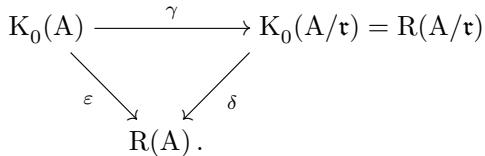
\includegraphics[keepaspectratio]{images/part002_05770a86.jpg}}

We denote the (finite) set of classes of simple A-modules by \(\mathcal{S}\) ; for every \(\lambda \in \mathcal{S}\) , choose a module \(S_{\lambda}\) of class \(\lambda\) and a projective cover \((P_{\lambda}, u_{\lambda})\) of \(S_{\lambda}\) (VIII, p.~175, Proposition 4). It follows from Proposition 6 of VIII, p.~176 that \(K_0(A)\) is a free \(\mathbf{Z}\) -module with basis the family \(([P_{\lambda}]_{\mathcal{P}(A)})_{\lambda \in \mathcal{S}}\) . Moreover, since \(S_{\lambda}\) is isomorphic to \(P_{\lambda} / \mathfrak{r}P_{\lambda}\) (VIII, p.~176), \(\gamma\) transforms the basis \(([P_{\lambda}]_{\mathcal{P}(A)})_{\lambda \in \mathcal{S}}\) of \(K_0(A)\) into the basis \(([S_{\lambda}])_{\lambda \in \mathcal{S}}\) of \(R(A / \mathfrak{r})\) . The isomorphism \(\delta\) transforms the basis \(([S_{\lambda}])_{\lambda \in \mathcal{S}}\) of \(R(A / \mathfrak{r})\) into the basis \(([S_{\lambda}])_{\lambda \in \mathcal{S}}\) of \(R(A)\) .

The Cartan matrix of A is the matrix \((a_{\lambda\mu})\) of the homomorphism of Z-modules \(\varepsilon: K_{0}(A) \to R(A)\) with respect to bases \(([P_{\lambda}]_{\mathcal{P}(A)})_{\lambda \in \mathcal{S}}\) of \(K_{0}(A)\) and \(([S_{\lambda}])_{\lambda \in \mathcal{S}}\) of \(R(A)\) . By definition, we have

\[
[ \mathrm{P} _ {\mu} ] = \sum_ {\lambda \in \mathcal {S}} a _ {\lambda \mu} [ \mathrm{S} _ {\lambda} ] \quad (\mu \in \mathcal {S})\tag{19}
\]

in the group R(A). In other words, \(a_{\lambda\mu}\) is the number of quotients isomorphic to \(S_{\lambda}\) in a Jordan--Hölder series of the A-module \(P_{\mu}\) .

Set \(\pi = \varepsilon \circ \gamma^{-1} \circ \delta^{-1}\) ; it is an endomorphism of the group R(A). If M is a finitely generated semisimple A-module and (P, \(u\) ) a projective cover of M, then we have \(\pi([M]) = [P]\) . By formula (19), the matrix of \(\pi\) with respect to the basis \(([S_{\lambda}])_{\lambda \in \mathcal{S}}\) of R(A) is simply the Cartan matrix of A.

\subsection{\texorpdfstring{Change of Rings for \(K_{0}(A)\)}{Change of Rings for K\_\{0\}(A)}}

Let A and B be rings. Let \(f: A \to B\) be a ring homomorphism. If P is a finitely generated projective A-module, then the B-module \(f^{*}(P) = B \otimes_{A} P\) is projective and finitely generated (II, §5, No.~2, p.~281, Corollary). The mapping \(P \mapsto \text{cl}(f^{*}(P))\) is a homomorphism from the monoid \(\mathcal{P}(A)\) to the monoid \(\mathcal{P}(B)\) and therefore defines a homomorphism \(f^{*}: K_{0}(A) \to K_{0}(B)\) characterized by the relation \(f^{*}([P]_{\mathcal{P}(A)}) = [f^{*}(P)]_{\mathcal{P}(B)}\) for every finitely generated projective A-module P. If \(g: B \to C\) is a second ring homomorphism, then it follows from the transitivity of the extension of scalars (II, §5, No.~1, p.~278, Proposition 2) that the homomorphisms \((g \circ f)^*\) and \(g^{*} \circ f^{*}\) from \(\mathrm{K}_{0}(\mathrm{A})\) to \(\mathrm{K}_{0}(\mathrm{C})\) are equal.

Suppose that \(f\) makes B into a finitely generated projective left A-module. Let Q be a finitely generated projective left B-module. Then Q is a direct factor of a finitely generated free B-module that is projective and finitely generated over A. Consequently, the A-module \(f_{*}(\mathrm{Q})\) obtained from Q by restriction of scalars is projective and finitely generated. As above, we deduce a homomorphism \(f_{*}: \mathrm{K}_{0}(\mathrm{B}) \to \mathrm{K}_{0}(\mathrm{A})\) characterized by the relation \(f_{*}([Q]_{\mathcal{P}(B)}) = [f_{*}(Q)]_{\mathcal{P}(A)}\) for every finitely generated projective B-module Q. If \(g: \mathrm{B} \to \mathrm{C}\) is a ring homomorphism that makes C into a finitely generated projective B-module, then the homomorphisms \((g \circ f)_{*}\) and \(f_{*} \circ g_{*}\) from \(\mathrm{K}_{0}(\mathrm{C})\) to \(\mathrm{K}_{0}(\mathrm{A})\) are equal.

\subsection{Frobenius Reciprocity}

Let A be a semisimple ring. Let f be a homomorphism from A to a semisimple ring B. Let S be a simple A-module and T a simple B-module, and let D and E be the centralizers of S and T, respectively. By Schur's lemma (VIII, p.~47, Corollary), D and E are fields. Let H be the set of A-linear homomorphisms from S to \(f_{*}(\mathrm{T})\) . We endow H with an (E,D)-bimodule structure with external laws \((e,u)\mapsto e\circ u\) and \((d,u)\mapsto u\circ d\) for \(e\in E\) , \(u\in H\) , \(d\in D\) .

PROPOSITION 11. --- a) The multiplicity \([f_{*}(\mathrm{T}):\mathrm{S}]\) of the simple A-module S in the semisimple A-module \(f_{*}(\mathrm{T})\) is equal to the dimension of H viewed as a right vector space over D.

\begin{enumerate}
\def\labelenumi{\alph{enumi})}
\setcounter{enumi}{1}
\tightlist
\item
  The multiplicity \([f^{*}(\mathrm{S}):\mathrm{T}]\) is finite and equal to the dimension of H viewed as a left vector space over E.
\end{enumerate}

Assertion a) follows from formula (11) of VIII, p.~72.

The B-module \(f^{*}(S)\) is semisimple and finitely generated, hence has finite length. By formula (12) of loc. cit., we have

\[
[ f ^ {*} (\mathrm{S}): \mathrm{T} ] = \dim_ {\mathrm{E}} \operatorname{Hom} _ {\mathrm{B}} (f ^ {*} (\mathrm{S}), \mathrm{T}).\tag{20}
\]

Now, in II, §5, No.~1, p.~277-278, formula (2) and Remark 2, we defined an E-linear bijection from \(\mathrm{Hom}_{\mathrm{A}}(\mathrm{S},f_{*}(\mathrm{T}))\) to \(\mathrm{Hom}_{\mathrm{B}}(f^{*}(\mathrm{S}),\mathrm{T})\) . Assertion b) then follows from formula (20).

COROLLARY (Frobenius reciprocity). --- Suppose that A and B are semisimple algebras that are finite-dimensional over a commutative field K and that f is K-linear. Then the K-vector spaces S, T, D, E, and H are finite-dimensional, and we have the equalities

\[
[ f _ {*} (\mathrm{T}): \mathrm{S} ] [ \mathrm{D}: \mathrm{K} ] = [ f ^ {*} (\mathrm{S}): \mathrm{T} ] [ \mathrm{E}: \mathrm{K} ] = [ \mathrm{H}: \mathrm{K} ].\tag{21}
\]

In particular, when K is algebraically closed, we have D = E = K and

\[
[ f _ {*} (\mathrm{T}): \mathrm{S} ] = [ f ^ {*} (\mathrm{S}): \mathrm{T} ] = [ \mathrm{H}: \mathrm{K} ].\tag{22}
\]

Since A-module S is simple, it is monogenous, and D is a linear subspace of \(\operatorname{Hom}_{\mathrm{K}}(\mathrm{S},\mathrm{S})\) ; hence S and D are finite-dimensional over K. For an analogous reason, T and E are finite-dimensional over K. Finally, H is a linear subspace of \(\operatorname{Hom}_{\mathrm{K}}(\mathrm{S},\mathrm{T})\) ; it is therefore also finite-dimensional. Formula (21) then follows from Proposition 11 because the dimension of H over K is equal to \([H:D][D:K]\) and to \([H:E][E:K]\) (II, §1, No.~13, p.~222, Proposition 25). By Theorem 1 of VIII, p.~47, if K is algebraically closed, we have D = E = K. The second part of the corollary then follows from the first.

Let \(\mathrm{A}\) and \(\mathrm{B}\) be semisimple algebras that are finite-dimensional over a commutative field \(\mathrm{K}\) , and let \(f\) be a homomorphism of \(\mathrm{K}\) -algebras from \(\mathrm{A}\) to \(\mathrm{B}\) .

Let \(\mathcal{S}(\mathrm{A})\) be the set of classes of simple A-modules; for every \(\lambda \in \mathcal{S}(\mathrm{A})\) , let \(\mathrm{S}_{\lambda}\) be a module of class \(\lambda\) and \(\mathrm{D}_{\lambda}\) its centralizer. Then \(\mathrm{D}_{\lambda}\) is an algebra of finite degree over \(\mathrm{K}\) ; we denote this degree by \(d_{\lambda}\) . We define \(\mathcal{S}(\mathrm{B})\) , \(\mathrm{T}_{\mu}\) , \(\mathrm{E}_{\mu}\) , and \(e_{\mu}\) for \(\mu\) in \(\mathcal{S}(\mathrm{B})\) analogously. The Grothendieck group \(\mathrm{K}_0(\mathrm{A})\) has the family \(([\mathrm{S}_{\lambda}])_{\lambda \in \mathcal{S}(\mathrm{A})}\) as a basis, and \(\mathrm{K}_0(\mathrm{B})\) has \(([\mathrm{T}_{\mu}])_{\mu \in \mathcal{S}(\mathrm{B})}\) as a basis. Let \((a_{\mu \lambda})\) be the matrix of \(f^{*}: \mathrm{K}_{0}(\mathrm{A}) \to \mathrm{K}_{0}(\mathrm{B})\) and \((b_{\lambda \mu})\) the matrix of \(f_{*}: \mathrm{K}_{0}(\mathrm{B}) \to \mathrm{K}_{0}(\mathrm{A})\) with respect to these bases. By definition, we have

\[
a _ {\mu \lambda} = [ f ^ {*} (\mathrm{S} _ {\lambda}): \mathrm{T} _ {\mu} ], \qquad b _ {\lambda \mu} = [ f _ {*} (\mathrm{T} _ {\mu}): \mathrm{S} _ {\lambda} ]\tag{23}
\]

for \(\lambda\) in \(\mathcal{S}(\mathrm{A})\) and \(\mu\) in \(\mathcal{S}(\mathrm{B})\) . We denote the dimension of the vector space \(\mathrm{Hom}_{\mathrm{A}}(\mathrm{S}_{\lambda}, f_{*}(\mathrm{T}_{\mu}))\) over the field K by \(h_{\lambda \mu}\) . By the corollary above, we have

\[
h _ {\lambda \mu} = e _ {\mu} a _ {\mu \lambda} = d _ {\lambda} b _ {\lambda \mu}.\tag{24}
\]

When the field K is algebraically closed, we have \(d_{\lambda} = e_{\mu} = 1\) ; consequently, we have

\[
a _ {\mu \lambda} = b _ {\lambda \mu} = h _ {\lambda \mu}.\tag{25}
\]

In other words, the matrices of \(f_{*}\) and \(f^{*}\) with respect to the given bases of \(\mathrm{K}_0(\mathrm{A})\) and \(\mathrm{K}_0(\mathrm{B})\) are each other's transposes.

\subsection{The Case of Simple Rings}

Let A and B be simple rings and f a homomorphism from A to B. Let S be a simple A-module and T a simple B-module. We set

\[
i (f) = [ f ^ {*} (\mathrm{S}): \mathrm{T} ] = \mathrm{long} _ {\mathrm{B}} (f ^ {*} (\mathrm{S}));\tag{26}
\]

we call the cardinal \(i(f)\) the index of f.~When A is a subring of B and f is the canonical injection of A into B, we write \(i(\mathrm{B},\mathrm{A})\) instead of \(i(f)\) , and we call this cardinal the index of A in B. We define the height \(h(f)\) of f analogously:

\[
h (f) = [ f _ {*} (\mathrm{T}): \mathrm{S} ] = \mathrm{long} _ {\mathrm{A}} (f _ {*} (\mathrm{T})).\tag{27}
\]

When A is a subring of B and f the canonical injection of A into B, we write \(h(\mathrm{B}, \mathrm{A})\) for \(h(f)\) , and we call it the height of A in B.

The A-module S is monogenous, hence so is the B-module \(f^{*}(\mathrm{S}) = \mathrm{B} \otimes_{\mathrm{A}} \mathrm{S}\) . It follows that \(i(f)\) is finite and therefore that it is an integer. Let M be an A-module. Denote its length by a; then M is isomorphic to \(\mathrm{S}^{(\mathfrak{a})}\) . Consequently, the B-module \(f_{*}(\mathrm{M})\) is isomorphic to \(f_{*}(\mathrm{S})^{(\mathfrak{a})}\) . By the definition of \(i(f)\) , we therefore have

\[
\mathrm{long} _ {\mathrm{B}} (f ^ {*} (\mathrm{M})) = i (f) \mathrm{long} _ {\mathrm{A}} (\mathrm{M}).\tag{28}
\]

The Z-modules \(K_{0}(A)\) and \(K_{0}(B)\) are free of dimension 1, with respective bases {[}S{]} and {[}T{]}, and we have

\[
f ^ {*} ([ \mathrm{S} ]) = i (f) [ \mathrm{T} ].\tag{29}
\]

Let us take, in particular, \(M = A_{s}\) ; then \(f^{*}(A_{s}) = B \otimes_{A} A_{s}\) is isomorphic to \(B_{s}\) (II, §3, No.~4, p.~249), so

\[
i (f) = \mathrm{long(B)} / \mathrm{long(A)}.\tag{30}
\]

By Wedderburn's theorem (VIII, p.~120, Theorem 1), there exist integers \(m \geqslant 1\) and \(n \geqslant 1\) and fields D and E such that A is isomorphic to \(\mathbf{M}_m(\mathrm{D})\) and B to \(\mathbf{M}_n(\mathrm{E})\) . By formula (30), we have \(i(f) = n / m\) ; in particular, \(m\) divides \(n\) .

Let N be an B-module; denote its length by a. Then N is isomorphic to \(\mathrm{T}^{(\mathfrak{a})}\) , so the A-module \(f_{*}(\mathrm{N})\) is isomorphic to \(f_{*}(\mathrm{T})^{(\mathfrak{a})}\) ; by the definition of \(h(f)\) , we have

\[
\mathrm{long} _ {\mathrm{A}} (f _ {*} (\mathrm{N})) = h (f) \mathrm{long} _ {\mathrm{B}} (\mathrm{N}).\tag{31}
\]

We have seen (VIII, p.~124, Proposition 5) that f makes B into a free A-module and that all bases of this module have the same cardinal, denoted by \([B:A]_{s}\) and called the (left) degree of B over A. The A-module \(f_{*}(B_{s})\) is isomorphic to \(A_{s}^{[B:A]_{s}}\) , so has length \([B:A]_{s}\) long(A). By formula (30) and formula (31) applied to the specific case \(N=B_{s}\) , we therefore have

\[
[ \mathrm{B}: \mathrm{A} ] _ {s} = i (f) h (f).\tag{32}
\]

Now suppose that B is a finitely generated A-module, that is, that \([B:A]_{s}\) is finite. Then \(h(f)\) is finite by formula (32). We defined (VIII, p.~202) a group homomorphism \(f_{*}\) from \(K_{0}(B)\) to \(K_{0}(A)\) ; we have

\[
f _ {*} ([ \mathrm{T} ]) = h (f) [ \mathrm{S} ].\tag{33}
\]

Suppose that A and B are finite-dimensional algebras over a commutative field K and that f is K-linear. As before, there exist integers \(m \geqslant 1\) and \(n \geqslant 1\) , K-algebras D and E that are fields, and K-algebra isomorphisms from A to \(\mathbf{M}_{m}(\mathrm{D})\) and from B to \(\mathbf{M}_{n}(\mathrm{E})\) . Set \(d = [D : K]\) and \(e = [E : K]\) . We then have the relations

\[
[ \mathrm{A}: \mathrm{K} ] = m ^ {2} d, \qquad [ \mathrm{B}: \mathrm{K} ] = n ^ {2} e, \qquad [ \mathrm{B}: \mathrm{A} ] _ {s} = \frac {n ^ {2} e}{m ^ {2} d}
\]

and, by formulas (30) and (32), the relations

\[
i (f) = \frac {n}{m}, \qquad h (f) = \frac {n e}{m d}.
\]

When the field \(\mathrm{K}\) is algebraically closed, we have \(d = e = 1\) and therefore \(i(f) = h(f)\) and \([\mathrm{B}:\mathrm{A}]_s = i(f)^2\) .

Let A, B, and C be simple rings, and let \(f: A \to B\) and \(g: B \to C\) be homomorphisms. Let S be a simple A-module. The C-modules \((g \circ f)^{*}(S)\) and \(g^{*}(f^{*}(S))\) are isomorphic; therefore, by formulas (26) and (28), we have

\[
i (g \circ f) = \operatorname{long} _ {\mathrm{C}} \left(g ^ {*} \left(f ^ {*} (\mathrm{S})\right)\right) = i (g) \operatorname{long} _ {\mathrm{B}} \left(f ^ {*} (\mathrm{S})\right) = i (g) i (f).
\]

We can prove the equality \(h(g \circ f) = h(g)h(f)\) likewise. When A is a subring of B and B is a subring of C, and we take the canonical injections for f and g, these equalities give

\[
i (\mathrm{C}, \mathrm{A}) = i (\mathrm{C}, \mathrm{B}) i (\mathrm{B}, \mathrm{A}), \qquad h (\mathrm{C}, \mathrm{A}) = h (\mathrm{C}, \mathrm{B}) h (\mathrm{B}, \mathrm{A}).\tag{34}
\]

PROPOSITION 12. --- Let B be a simple ring and A a simple subring of B. Suppose that B is a finitely generated left A-module. Let M be a nonzero finitely generated left B-module. Set \(A' = \text{End}_{A}(M)\) and \(B' = \text{End}_{B}(M)\) . Then \(B'\) is a subring of \(A'\) , the rings \(A'\) and \(B'\) are simple, \(A'\) is a finitely generated left \(B'\) -module, and we have the equalities

\[
i (\mathrm{A} ^ {\prime}, \mathrm{B} ^ {\prime}) = h (\mathrm{B}, \mathrm{A}), \quad h (\mathrm{A} ^ {\prime}, \mathrm{B} ^ {\prime}) = i (\mathrm{B}, \mathrm{A}), \quad [ \mathrm{A} ^ {\prime}: \mathrm{B} ^ {\prime} ] _ {s} = [ \mathrm{B}: \mathrm{A} ] _ {s}.
\]

By Proposition 4 of VIII, p.~123, the ring \(\mathrm{A}'\) is simple, \(\mathrm{M}\) is an \(\mathrm{A}'\) -module of finite length, and we have

\[
\mathrm{long} _ {\mathrm{A}} (\mathrm{M}) = \mathrm{long} (\mathrm{A} ^ {\prime}), \quad \mathrm{long} _ {\mathrm{A} ^ {\prime}} (\mathrm{M}) = \mathrm{long} (\mathrm{A}).
\]

For the same reasons, the ring \(B'\) is simple, and we have

\[
\operatorname{long} _ {\mathrm{B}} (\mathrm{M}) = \operatorname{long} \left(\mathrm{B} ^ {\prime}\right), \quad \operatorname{long} _ {\mathrm{B} ^ {\prime}} (\mathrm{M}) = \operatorname{long} (\mathrm{B}).
\]

By formulas (31) and (30), we therefore have

\[
h (\mathrm{B}, \mathrm{A}) = \operatorname{long} _ {\mathrm{A}} (\mathrm{M}) / \operatorname{long} _ {\mathrm{B}} (\mathrm{M}) = \operatorname{long} \left(\mathrm{A} ^ {\prime}\right) / \operatorname{long} \left(\mathrm{B} ^ {\prime}\right) = i \left(\mathrm{A} ^ {\prime}, \mathrm{B} ^ {\prime}\right);
\]

the equality \(h(\mathrm{A}^{\prime},\mathrm{B}^{\prime}) = i(\mathrm{B},\mathrm{A})\) can be established analogously. From this, we deduce

\[
[ \mathrm{A} ^ {\prime}: \mathrm{B} ^ {\prime} ] _ {s} = i (\mathrm{A} ^ {\prime}, \mathrm{B} ^ {\prime}) h (\mathrm{A} ^ {\prime}, \mathrm{B} ^ {\prime}) = h (\mathrm{B}, \mathrm{A}) i (\mathrm{B}, \mathrm{A}) = [ \mathrm{B}: \mathrm{A} ] _ {s}
\]

using formula (32). In particular, \(A'\) is a finitely generated left \(B'\) -module.

\BourbakiExercises{Exercises}

\begin{enumerate}
\def\labelenumi{\arabic{enumi})}
\tightlist
\item
  Let p be a prime number. Denote by C the set of classes of Z-modules of the form \((\mathbf{Z}/p^{2}\mathbf{Z})^{n} \oplus (\mathbf{Z}/p^{3}\mathbf{Z})^{m}\) for \(n, m \in N\) .
\end{enumerate}

\begin{enumerate}
\def\labelenumi{\alph{enumi})}
\item
  Prove that \(\mathcal{C}\) is additive but not hereditary. What is the smallest hereditary set \(\mathcal{H}\) containing \(\mathcal{C}\) ?
\item
  Prove that every short exact sequence of modules of type C splits. Describe the group \(\mathrm{K}(\mathcal{C})\) .
\item
  Construct an exact sequence
\end{enumerate}

\[
0 \to \mathrm{M} _ {0} \to \mathrm{M} _ {1} \to \mathrm{M} _ {2} \to \mathrm{M} _ {3} \to \mathrm{M} _ {4} \to 0
\]

of modules of type C such that the classes of \(M_{0} \oplus M_{2} \oplus M_{4}\) and \(M_{1} \oplus M_{3}\) in \(\mathrm{K}(\mathcal{C})\) are distinct.

\begin{enumerate}
\def\labelenumi{\alph{enumi})}
\setcounter{enumi}{3}
\tightlist
\item
  Is the natural homomorphism from \(\mathrm{K}(\mathcal{C})\) to \(\mathrm{K}(\mathcal{H})\) injective?
\end{enumerate}

\begin{enumerate}
\def\labelenumi{\arabic{enumi})}
\setcounter{enumi}{1}
\item
  Let \(\mathrm{A}\) be a ring and \(a\) and \(b\) two elements of \(\mathrm{A}\) such that \(ab = 1\) and \(ba \neq 1\) . Prove that the A-module \(\mathrm{A}(1 - ba)\) is projective and that it is stably isomorphic to the zero A-module. More precisely, prove that the A-modules \(\mathrm{A}_s\) and \(\mathrm{A}(1 - ba) \oplus \mathrm{A}_s\) are isomorphic.
\item
  Let A and B be rings. Determine the Grothendieck groups \(R(A \times B)\) and \(K_{0}(A \times B)\) of \(A \times B\) in terms of those of A and B.
\item
  Let A and B be Morita equivalent rings. Prove that the groups R(A) and R(B) are isomorphic. Do the same for \(K_{0}(A)\) and \(K_{0}(B)\) .
\item
  Let A be a ring. Denote by \(\mathcal{I}(A)\) the set of pairs \((n,p)\) with n an integer and p an idempotent in \(M_{n}(A)\) . Define a law of addition on \(\mathcal{I}(A)\) by setting \((m,p)+(n,q)=(m+n,\begin{pmatrix} p & 0 \\ 0 & q \end{pmatrix})\) .
\end{enumerate}

\begin{enumerate}
\def\labelenumi{\alph{enumi})}
\item
  Let \(\mathcal{P}(A^{\circ})\) be the monoid of classes of finitely generated projective right A-modules. Let \(\varphi: \mathcal{I}(A) \to \mathcal{P}(A^{\circ})\) be the mapping defined by \(\varphi(n,p) = \operatorname{cl}(\operatorname{Im}p)\) . Prove that \(\varphi\) is a surjective homomorphism and that elements \((m,p)\) and \((n,q)\) of \(\mathcal{I}(A)\) have the same image by \(\varphi\) if and only if there exist \(a \in M_{m,n}(A)\) and \(b \in M_{n,m}(A)\) such that ab = p and ba = q.
\item
  Deduce that the groups \(K_{0}(A)\) and \(K_{0}(A^{\circ})\) are isomorphic.
\end{enumerate}

\begin{enumerate}
\def\labelenumi{\arabic{enumi})}
\setcounter{enumi}{5}
\tightlist
\item
  Let A be a ring, G an abelian group, and T: A → G a tracial mapping (VIII, p.~115, Exercise 3). For any finitely generated projective right A-module P, denote by
\end{enumerate}

\[
\mathrm{T} _ {\mathrm{P}}: \operatorname{End} _ {\mathrm{A}} (\mathrm{P} \oplus \mathrm{A} _ {d}) \longrightarrow \mathrm{G}
\]

the unique tracial mapping that extends T (loc. cit.) and by \(\pi_{P}\) the projector of \(\operatorname{End}_{\mathrm{A}}(\mathrm{P} \oplus \mathrm{A}_{d})\) with image P and kernel \(A_{d}\) . Construct a group homomorphism \(\widetilde{\mathrm{T}} : \mathrm{K}_{0}(\mathrm{A}) \to \mathrm{G}\) such that \(\widetilde{\mathrm{T}}([\mathrm{P}]) = \mathrm{T}_{\mathrm{P}}(\pi_{\mathrm{P}})\) for every finitely generated projective right A-module P.

\begin{enumerate}
\def\labelenumi{\arabic{enumi})}
\setcounter{enumi}{6}
\tightlist
\item
  Let I be a right directed set, \((\mathrm{A}_{i}, f_{ji})\) a direct system of rings, and A its limit. Prove that \(\mathrm{K}_{0}(\mathrm{A})\) is the limit of the direct system of groups \((\mathrm{K}_{0}(\mathrm{A}_{i}), f_{ji}^{*})\) .
\end{enumerate}

¶ 8) Let A, B, and C be rings and \(f: \mathrm{A} \to \mathrm{C}\) and \(g: \mathrm{B} \to \mathrm{C}\) ring homomorphisms; suppose that \(f\) is surjective. Consider the subring D of \(\mathrm{A} \times \mathrm{B}\) consisting of the pairs \((a, b)\) such that \(f(a) = g(b)\) . Let M be an A-module, N a B-module, and \(u\) a C-isomorphism from \(\mathrm{C} \otimes_{\mathrm{A}} \mathrm{M}\) to \(\mathrm{C} \otimes_{\mathrm{B}} \mathrm{N}\) . Denote by P the D-submodule of \(\mathrm{M} \times \mathrm{N}\) consisting of the pairs \((m, n)\) such that \(u(1 \otimes m) = 1 \otimes n\) .

\begin{enumerate}
\def\labelenumi{\alph{enumi})}
\item
  Suppose that the modules M and N admit finite bases \((e_{i})_{i\in\mathrm{I}}\) and \((f_{j})_{j\in\mathrm{J}}\) and that the matrix of u in the bases \((1\otimes e_{i})\) and \((1\otimes f_{j})\) is the image of an invertible matrix \((a_{ji})\) with entries in A. Prove that the D-module P is free; more precisely, the elements \((e_{i},\sum_{j}a_{ji}f_{j})_{i\in\mathrm{I}}\) form a basis of P.
\item
  Let p and q be integers and \(X \in \mathbf{M}_{p,q}(\mathrm{C})\) and \(Y \in \mathbf{M}_{q,p}(\mathrm{C})\) matrices such that \(XY = I_{p}\) and \(YX = I_{q}\) . Prove that the square matrix \(\begin{pmatrix} X & 0 \\ 0 & Y \end{pmatrix}\) is the image of an invertible matrix with entries in A, using the identity
\end{enumerate}

\[
\left( \begin{array}{c c} X & 0 \\ 0 & Y \end{array} \right) = \left( \begin{array}{c c} I _ {p} & X \\ 0 & I _ {q} \end{array} \right) \left( \begin{array}{c c} I _ {p} & 0 \\ - Y & I _ {q} \end{array} \right) \left( \begin{array}{c c} I _ {p} & X \\ 0 & I _ {q} \end{array} \right) \left( \begin{array}{c c} 0 & - I _ {p} \\ I _ {q} & 0 \end{array} \right).
\]

\begin{enumerate}
\def\labelenumi{\alph{enumi})}
\setcounter{enumi}{2}
\item
  Suppose that the modules M and N are free and finitely generated. Deduce from a) and b) that the D-module P is projective and finitely generated.
\item
  Suppose that M and N are projective and finitely generated. Construct an A-module \(M'\) and a B-module \(N'\) such that \(M \oplus M'\) and \(N \oplus N'\) are free and finitely generated and that the C-modules \(C \otimes_{A} M'\) and \(C \otimes_{B} N'\) are isomorphic. Deduce that the D-module P is projective and finitely generated.
\item
  Prove that the canonical homomorphisms \(A \otimes_{D} P \to M\) and \(B \otimes_{D} P \to N\) deduced from the two projections are bijective (reduce as above to the case when the conditions of a) are satisfied).
\item
  Conversely, let \(P'\) be a finitely generated projective D-module; set \(M' = A \otimes_{D} P'\) and \(N' = B \otimes_{D} P'\) , and denote by \(u' : C \otimes_{A} M' \to C \otimes_{B} N'\) the canonical isomorphism. Prove that the canonical homomorphism from \(P'\) to \(M' \times N'\) induces a D-linear isomorphism from \(P'\) to the D-module associated with \((M', N', u')\) .
\end{enumerate}

\(g)\) Denote by \(\varphi_0:\mathrm{K}_0(\mathrm{D})\to \mathrm{K}_0(\mathrm{A})\times \mathrm{K}_0(\mathrm{B})\) and \(\psi_0:\mathrm{K}_0(\mathrm{A})\times \mathrm{K}_0(\mathrm{B})\to \mathrm{K}_0(\mathrm{C})\) the homomorphisms such that

\[
\varphi_ {0} ([ \mathrm{P} ]) = ([ \mathrm{A} \otimes_ {\mathrm{D}} \mathrm{P} ], [ \mathrm{B} \otimes_ {\mathrm{D}} \mathrm{P} ]) \quad \text { and } \quad \psi_ {0} ([ \mathrm{M} ], [ \mathrm{N} ]) = [ \mathrm{C} \otimes_ {\mathrm{A}} \mathrm{M} ] - [ \mathrm{C} \otimes_ {\mathrm{B}} \mathrm{N} ].
\]

Prove that the sequence

\[
\mathrm{K} _ {0} (\mathrm{D}) \xrightarrow {\varphi_ {0}} \mathrm{K} _ {0} (\mathrm{A}) \times \mathrm{K} _ {0} (\mathrm{B}) \xrightarrow {\psi_ {0}} \mathrm{K} _ {0} (\mathrm{C})
\]

is exact. Prove that if, moreover, there exists a ring homomorphism \(s: C \to A\) such that \(f \circ s = Id_{C}\) , then \(\varphi_{0}\) is injective and \(\psi_{0}\) is surjective.

\begin{enumerate}
\def\labelenumi{\arabic{enumi})}
\setcounter{enumi}{8}
\tightlist
\item
  Let A be a pseudoring, that is, an associative not necessarily unital Z-algebra, and \(\widetilde{A}\) the Z-algebra deduced from A by adjoining a unit element (III, §1, No.~2, p.~431); the set \(\widetilde{\mathrm{A}}\) is equal to \(\mathbf{Z} \times \mathrm{A}\) . Denote the homomorphism \((n, a) \mapsto n\) by \(\varepsilon : \widetilde{\mathrm{A}} \to \mathbf{Z}\) , and denote the kernel of the homomorphism \(\varepsilon^{*} : \mathrm{K}_{0}(\widetilde{\mathrm{A}}) \to \mathrm{K}_{0}(\mathbf{Z})\) associated with \(\varepsilon\) by \(\mathrm{K}_{0}(\mathrm{A})\) .
\end{enumerate}

\begin{enumerate}
\def\labelenumi{\alph{enumi})}
\item
  Prove that if A is unital, then \(\tilde{A}\) is isomorphic to the product ring \(Z \times A\) and the definition of \(K_{0}(A)\) is compatible with that given in No.~8.
\item
  Let A and B be pseudorings and \(f: \mathrm{A} \to \mathrm{B}\) a homomorphism. Let \(\widetilde{f}: \widetilde{\mathrm{A}} \to \widetilde{\mathrm{B}}\) be the ring homomorphism defined by \(\widetilde{f}((n, a)) = (n, f(a))\) . Prove that \(\widetilde{f}^*\) maps \(\mathrm{K}_0(\mathrm{A})\) into \(\mathrm{K}_0(\mathrm{B})\) . Denote the homomorphism deduced from \(\widetilde{f}^*\) by \(f^*: \mathrm{K}_0(\mathrm{A}) \to \mathrm{K}_0(\mathrm{B})\) . c) Suppose that \(f\) is surjective; denote its kernel by \(\mathfrak{a}\) and the canonical injection of \(\mathfrak{a}\) into A by \(i\) . Show that the sequence
\end{enumerate}

\[
\mathrm{K} _ {0} (\mathfrak {a}) \xrightarrow {i ^ {*}} \mathrm{K} _ {0} (\mathrm{A}) \xrightarrow {f ^ {*}} \mathrm{K} _ {0} (\mathrm{B})
\]

is exact. If, moreover, there exists a homomorphism of pseudorings \(s: B \to A\) such that \(f \circ s = Id_{B}\) , then \(i^{*}\) is injective and \(f^{*}\) is surjective (apply Exercise 8 by first taking (A, A, B) and then (D, Z, A) for the triple (A, B, C)).

\begin{enumerate}
\def\labelenumi{\alph{enumi})}
\setcounter{enumi}{3}
\tightlist
\item
  Prove that the conclusions of Exercises 7 and 8 extend to the case of pseudorings. e) Denote by \(\mathbf{M}_{\infty}(\mathrm{A})\) the pseudoring of \(\mathbf{N} \times \mathbf{N}\) matrices with entries in A having only finitely many nonzero entries. Let \(f: \mathrm{A} \to \mathbf{M}_{\infty}(\mathrm{A})\) be the mapping that sends \(a \in \mathrm{A}\) to the matrix \((b_{ij})\) with \(b_{00} = a\) and \(b_{ij} = 0\) if \((i,j) \neq (0,0)\) . Prove that \(f^{*}\) is an isomorphism from \(\mathrm{K}_0(\mathrm{A})\) to \(\mathrm{K}_0(\mathbf{M}_{\infty}(\mathrm{A}))\) (use Exercises 4 and 7).
\end{enumerate}

\begin{enumerate}
\def\labelenumi{\arabic{enumi})}
\setcounter{enumi}{9}
\tightlist
\item
  Let A be a ring. Denote by \(\mathbf{GL}_{\infty}(\mathrm{A})\) the subgroup of \(\mathbf{GL}(\mathrm{A}^{(\mathbf{N})})\) consisting of the matrices X such that X - I has only finitely many nonzero entries, and denote by \(\mathrm{E}(\mathrm{A})\) the subgroup of \(\mathbf{GL}_{\infty}(\mathrm{A})\) generated by the matrices \(I + \lambda E_{ij}\) for i, j in N with \(i \neq j\) and \(\lambda \in A\) ; it is the derived group of \(\mathbf{GL}_{\infty}(\mathrm{A})\) (II, §10, p.~422, Exercise 15). Denote the quotient group \(\mathbf{GL}_{\infty}(\mathrm{A}) / \mathrm{E}(\mathrm{A})\) by \(\mathrm{K}_{1}(\mathrm{A})\) ; its group law is written additively. Every ring homomorphism \(f : A \to B\) induces a group homomorphism \(f^{*} : K_{1}(A) \to K_{1}(B)\) .
\end{enumerate}

\begin{enumerate}
\def\labelenumi{\alph{enumi})}
\item
  For any integer \(n \geqslant 1\) , let \(\iota_{n} : \mathbf{GL}_{n}(\mathrm{A}) \to \mathrm{K}_{1}(\mathrm{A})\) be the homomorphism that sends \(X \in \mathbf{GL}_{n}(\mathrm{A})\) to the class of the matrix \(\begin{pmatrix} X & 0 \\ 0 & I \end{pmatrix}\) . Prove that if the ring A is local, then \(\iota_{n}\) is surjective for every n (use Exercise 17 of VIII, p.~42).
\item
  Suppose that the ring A is commutative. Construct a surjective homomorphism \(d_{\mathrm{A}} : \mathrm{K}_{1}(\mathrm{A}) \to \mathrm{A}^{*}\) such that \(d_{A} \circ \iota_{n} = det\) for every n.~If, moreover, A is local or Euclidean, then the homomorphisms \(d_{A}\) and \(\iota_{1}\) are inverse bijections.
\item
  Let I be a right directed set, \((\mathrm{A}_{i}, f_{ji})\) a direct system of rings, and A its limit. Prove that \(\mathrm{K}_{1}(\mathrm{A})\) is the limit of the direct system of groups \((\mathrm{K}_{1}(\mathrm{A}_{i}), f_{ji}^{*})\) .
\end{enumerate}

¶ 11) Take the assumptions and notation of Exercise 8. Denote by \(f': \mathrm{D} \to \mathrm{B}\) and \(g': \mathrm{D} \to \mathrm{A}\) the homomorphisms deduced from the two projections and by

\[
\varphi_ {1}: \mathrm{K} _ {1} (\mathrm{D}) \rightarrow \mathrm{K} _ {1} (\mathrm{A}) \times \mathrm{K} _ {1} (\mathrm{B}) \quad \text { and } \quad \psi_ {1}: \mathrm{K} _ {1} (\mathrm{A}) \times \mathrm{K} _ {1} (\mathrm{B}) \rightarrow \mathrm{K} _ {1} (\mathrm{C})
\]

the mappings defined by \(\varphi_1(z) = (g'^* (z), f'^* (z))\) and \(\psi_1(x,y) = f^* (x) - g^* (y)\) .

\begin{enumerate}
\def\labelenumi{\alph{enumi})}
\tightlist
\item
  Prove that the sequence
\end{enumerate}

\[
\mathrm{K} _ {1} (\mathrm{D}) \xrightarrow {\varphi_ {1}} \mathrm{K} _ {1} (\mathrm{A}) \times \mathrm{K} _ {1} (\mathrm{B}) \xrightarrow {\psi_ {1}} \mathrm{K} _ {1} (\mathrm{C})
\]

is exact (observe that \(f(\mathrm{E}(\mathrm{A})) = \mathrm{E}(\mathrm{C})\) ). Prove that if, moreover, there exists a ring homomorphism \(s : C \to A\) such that \(f \circ s = Id_{C}\) , then \(\psi_{1}\) is surjective.

\begin{enumerate}
\def\labelenumi{\alph{enumi})}
\setcounter{enumi}{1}
\item
  For any integer n and any element g of \(\mathbf{GL}_{n}(\mathrm{C})\) , denote by \(P_{g}\) the projective D-module associated with the modules \(A^{n}\) and \(B^{n}\) and the isomorphism from \(C \otimes_{A} A^{n}\) to \(C \otimes_{B} B^{n}\) with matrix g (Exercise 8). Construct a homomorphism \(\partial : K_{1}(\mathrm{C}) \to K_{0}(\mathrm{D})\) such that \(\partial \circ \iota_{n}(g) = [\mathrm{P}_{g}] - [\mathrm{D}_{s}^{n}]\) for every integer n and every element g of \(\mathbf{GL}_{n}(\mathrm{C})\) .
\item
  Prove that the sequence
\end{enumerate}

\[
\mathrm{K} _ {1} (\mathrm{D}) \xrightarrow {\varphi_ {1}} \mathrm{K} _ {1} (\mathrm{A}) \times \mathrm{K} _ {1} (\mathrm{B}) \xrightarrow {\psi_ {1}} \mathrm{K} _ {1} (\mathrm{C}) \xrightarrow {\partial} \mathrm{K} _ {0} (\mathrm{D}) \xrightarrow {\varphi_ {0}} \mathrm{K} _ {0} (\mathrm{A}) \times \mathrm{K} _ {0} (\mathrm{B}) \xrightarrow {\psi_ {0}} \mathrm{K} _ {0} (\mathrm{C})
\]

is exact.

\begin{enumerate}
\def\labelenumi{\arabic{enumi})}
\setcounter{enumi}{11}
\tightlist
\item
  Let \(f: \mathrm{A} \to \mathrm{B}\) be a surjective ring homomorphism, \(\mathfrak{a}\) its kernel, and \(i\) the canonical injection of \(\mathfrak{a}\) into \(\mathrm{A}\) . Construct a homomorphism \(\partial: \mathrm{K}_1(\mathrm{B}) \to \mathrm{K}_0(\mathfrak{a})\) such that the sequence
\end{enumerate}

\[
\mathrm{K} _ {1} (\mathrm{A}) \xrightarrow {f ^ {*}} \mathrm{K} _ {1} (\mathrm{B}) \xrightarrow {\partial} \mathrm{K} _ {0} (\mathfrak {a}) \xrightarrow {i ^ {*}} \mathrm{K} _ {0} (\mathrm{A}) \xrightarrow {f ^ {*}} \mathrm{K} _ {0} (\mathrm{B})
\]

is exact (argue as in Exercise 11, c)).

\begin{enumerate}
\def\labelenumi{\arabic{enumi})}
\setcounter{enumi}{12}
\item
  Denote by \(\mathcal{C}\) (resp. \(\mathcal{D}\) ) the set of classes of \(\mathbf{Z}\) -modules of finite length (resp. finitely generated \(\mathbf{Z}\) -modules). Show that the group homomorphism \(\gamma_{\mathcal{D},\mathcal{C}}\) from \(\mathrm{K}(\mathcal{C})\) to \(\mathrm{K}(\mathcal{D})\) is zero.
\item
  Let K be a commutative field of characteristic different from 2. Write
\end{enumerate}

\[
\mathrm{A} = \mathrm{K} [ \mathrm{X}, \mathrm{Y}, \mathrm{Z} ] / (\mathrm{X} ^ {2} + \mathrm{Y} ^ {2} + \mathrm{Z} ^ {2} - 1).
\]

Let M be the A-module \(\mathrm{A}^{3}/\mathrm{A}(\overline{\mathrm{X}},\overline{\mathrm{Y}},\overline{\mathrm{Z}})\) , where \(\overline{X}\) , \(\overline{Y}\) , and \(\overline{Z}\) denote the respective images of X, Y, and Z in A. Show that \(M\oplus A\) is a free A-module but that M is not a free module.

\section{Tensor Products of Semisimple Modules}

In this section, the letter K denotes a commutative field. If E and F are vector spaces over K, then we denote the tensor product \(E \otimes_{K} F\) by \(E \otimes F\) .

\subsection{Semisimple Modules over Tensor Products of Algebras}

In this subsection, we consider K-algebras \(A_{1}\) and \(A_{2}\) ; we denote the algebra \(A_{1} \otimes A_{2}\) by A.

PROPOSITION 1. --- Let \(M_{1}\) be an \(A_{1}\) -module and \(M_{2}\) an \(A_{2}\) -module, neither reduced to 0. If the module \(M = M_{1} \otimes M_{2}\) over the ring \(A = A_{1} \otimes A_{2}\) is simple (resp. isotypical, semisimple), then the \(A_{1}\) -module \(M_{1}\) and the \(A_{2}\) -module \(M_{2}\) are simple (resp. isotypical, semisimple).

Suppose that M is a semisimple A-module. Let \(N_{1}\) be an \(A_{1}\) -submodule of \(M_{1}\) . Denote the canonical image of \(N_{1} \otimes M_{2}\) in the A-module M by N. By Corollary 2 of VIII, p.~56, there exists an A-linear projector p in M with image N. By assumption, we have \(M_{2} \neq 0\) ; we can therefore choose an element m of \(M_{2}\) and a linear form \(\varphi\) on the K-vector space \(M_{2}\) such that \(\varphi(m) = 1\) (II, §7, No.~5, p.~302, Corollary 2). Let u be the mapping from \(M_{1}\) to M defined by \(u(m_{1}) = m_{1} \otimes m\) , and let v be the K-linear mapping from M to \(M_{1}\) characterized by \(v(m_{1} \otimes m_{2}) = \varphi(m_{2})m_{1}\) . Set \(q = v \circ p \circ u\) . The mapping \(q : M_{1} \to M_{1}\) is \(A_{1}\) -linear, its image is contained in \(N_{1}\) , and we have \(q(n) = n\) for every \(n \in N_{1}\) . Consequently, q is a projector in \(M_{1}\) with image \(N_{1}\) . We have proved that \(M_{1}\) is a semisimple \(A_{1}\) -module (VIII, p.~56, Corollary 2).

Suppose that M is simple and that \(M_{1}\) is the direct sum of two \(A_{1}\) -submodules \(M_{1}^{\prime}\) and \(M_{1}^{\prime\prime}\) . Set \(M^{\prime}=M_{1}^{\prime}\otimes M_{2}\) and \(M^{\prime\prime}=M_{1}^{\prime\prime}\otimes M_{2}\) ; then M is the direct sum of the A-submodules \(M'\) and \(M''\) . Since M is simple, \(M'\) or \(M''\) must be reduced to 0; as we have \(M_{2} \neq 0\) by assumption, we have \(M_{1}' = 0\) or \(M_{1}'' = 0\) (II, §3, No.~7, p.~256, Corollary 2). This proves that \(M_{1}\) is a simple \(A_{1}\) -module.

Now suppose that M is an isotypical A-module. Let S and T be simple \(A_{1}\) -submodules of \(M_{1}\) . The A-modules \(S \otimes M_{2}\) and \(T \otimes M_{2}\) can then be identified with nonzero submodules of M. They are therefore isotypical of the same type as M. By Remark VIII, p.~61, there exists a nonzero A-linear mapping \(f : S \otimes M_{2} \to T \otimes M_{2}\) . The mapping f is, in particular, \(A_{1}\) -linear. Since the \(A_{1}\) -modules \(S \otimes M_{2}\) and \(T \otimes M_{2}\) are nonzero and isotypical of type S and T, respectively, S and T are isomorphic. This proves that \(M_{1}\) is an isotypical \(A_{1}\) -module.

PROPOSITION 2. --- Let S be a simple module over the ring \(A = A_{1} \otimes A_{2}\) , finite-dimensional over K. For \(i \in \{1, 2\}\) , there exists a simple \(A_{i}\) -module \(S_{i}\) such that the \(A_{i}\) -module S is isotypical of type \(S_{i}\) . The A-module S is isomorphic to a quotient of the A-module \(S_{1} \otimes S_{2}\) .

Since S is a nonzero \(A_{1}\) -module that is finite-dimensional over K, it has finite length over \(A_{1}\) and there exist a simple left \(A_{1}\) -module \(S_{1}\) and a nonzero \(A_{1}\) -linear mapping from \(S_{1}\) to S. We endow \(\mathrm{M}_{2} = \mathrm{Hom}_{\mathrm{A}_{1}}(\mathrm{S}_{1}, \mathrm{S})\) with a left \(A_{2}\) -module structure defined by the external law \((a_{2}, u) \mapsto (a_{2})_{\mathrm{S}} \circ u\) . We have \(M_{2} \neq 0\) by construction, and \(M_{2}\) is finite-dimensional over K. We can therefore find a simple left \(A_{2}\) -module \(S_{2}\) and a nonzero \(A_{2}\) -linear mapping \(\varphi : S_{2} \to M_{2}\) . We define a nonzero A-linear mapping \(\psi\) from \(S_{1} \otimes S_{2}\) to S by

\[
\psi (s _ {1} \otimes s _ {2}) = \varphi (s _ {2}) (s _ {1})\tag{1}
\]

for every \(s_{1} \in S_{1}\) and \(s_{2} \in S_{2}\) . Since S is a simple A-module and \(\psi\) is not zero, \(\psi\) is surjective and S is isomorphic to a quotient of \(S_{1} \otimes S_{2}\) . For \(i \in \{1, 2\}\) , the \(A_{i}\) -module \(S_{1} \otimes S_{2}\) is isotypical of type \(S_{i}\) , and therefore so is the \(A_{i}\) -module S (VIII, p.~61, Proposition 2).

For any K-algebra B, we denote by \(\mathcal{S}_{\mathrm{K}}(\mathrm{B})\) the set of classes of simple (VIII, p.~51) left B-modules that are finite-dimensional over K.

THEOREM 1. --- Suppose that the field K is algebraically closed.

\begin{enumerate}
\def\labelenumi{\alph{enumi})}
\item
  Let \(M_{1}\) be an \(A_{1}\) -module and \(M_{2}\) an \(A_{2}\) -module, both simple (resp. semisimple) and finite-dimensional over K. Then \(M_{1} \otimes M_{2}\) is a simple (resp. semisimple) module over the ring \(A_{1} \otimes A_{2}\) and is finite-dimensional over K.
\item
  The mapping from \(\mathcal{S}_{\mathrm{K}}(\mathrm{A}_1)\times \mathcal{S}_{\mathrm{K}}(\mathrm{A}_2)\) to \(\mathcal{S}_{\mathrm{K}}(\mathrm{A}_1\otimes \mathrm{A}_2)\) that sends \((\operatorname {cl}(\mathrm{S}_1),\operatorname {cl}(\mathrm{S}_2))\) to \(\operatorname {cl}(\mathrm{S}_1\otimes \mathrm{S}_2)\) , where \(\mathrm{S}_1\) (resp. \(\mathrm{S}_2\) ) is a simple \(\mathrm{A}_1\) -module (resp. \(\mathrm{A}_2\) -module) that is finite-dimensional over \(\mathrm{K}\) , is bijective.
\end{enumerate}

To prove part a), it suffices to consider the case when \(M_{1}\) and \(M_{2}\) are simple. Let \(M'\) be an A-submodule of \(M = M_{1} \otimes M_{2}\) ; it is an \(A_{1}\) -submodule of \(M_{1} \otimes M_{2}\) , stable under the set of endomorphisms of the form \(1_{M_{1}} \otimes u\) , where u runs through the set of homotheties of the \(A_{2}\) -module \(M_{2}\) . Since the field K is algebraically closed, Schur's lemma (VIII, p.~47, Theorem 1) implies that the commutant \(\operatorname{End}_{\mathrm{A}_{1}}(\mathrm{M}_{1})\) of \(M_{1}\) is equal to K. By Corollary 2 of VIII, p.~63, the A-submodule \(M'\) of \(M_{1} \otimes M_{2}\) is of the form \(M_{1} \otimes M_{2}'\) , where \(M_{2}'\) is an \(A_{2}\) -submodule of \(M_{2}\) . We have assumed that \(M_{2}\) is simple; we therefore have \(M_{2}' = 0\) or \(M_{2}' = M_{2}\) , that is, \(M' = 0\) or \(M' = M\) . Consequently, M is simple.

If S is a simple module over \(A_{1} \otimes A_{2}\) that is finite-dimensional over K, then it follows from Proposition 2 and part a) that S is isomorphic to a module of the form \(S_{1} \otimes S_{2}\) , where \(S_{1}\) (resp. \(S_{2}\) ) is a simple \(A_{1}\) -module (resp. \(A_{2}\) -module). Moreover, as an \(A_{i}\) -module, S is isotypical of type \(S_{i}\) , so the class of \(S_{i}\) only depends on that of S. This proves part b).

Remarks. --- 1) Assertion a) of Theorem 1 is no longer true when the field K is not assumed algebraically closed. We can give examples (VIII, p.~225, Exercise 4) where \(M_{i}\) is a simple \(A_{i}\) -module that is finite-dimensional over K, for \(i \in \{1, 2\}\) , and where the A-module \(M_{1} \otimes M_{2}\) is not semisimple or is semisimple but not simple.

\begin{enumerate}
\def\labelenumi{\arabic{enumi})}
\setcounter{enumi}{1}
\tightlist
\item
  There exists a homomorphism \(\varphi\) from \(\mathrm{R_K(A_1)\otimes_{\mathbf{Z}} R_K(A_2)}\) to \(\mathrm{R_K(A)}\) characterized by the relation \(\varphi ([\mathrm{M}_1]\otimes [\mathrm{M}_2]) = [\mathrm{M}_1\otimes \mathrm{M}_2]\) . This can be proved in the same way as Proposition 9 of VIII, p.~196. If the field \(K\) is algebraically closed, then \(\varphi\) is an isomorphism from \(\mathrm{R_K(A_1)\otimes_{\mathbf{Z}} R_K(A_2)}\) to \(\mathrm{R_K(A)}\) by Theorem 1, b) because for every K-algebra B, the \(\mathbf{Z}\) -module \(\mathrm{R_K(B)}\) is free with basis the family \(([\mathrm{S}])_{\mathrm{S}\in \mathcal{S}_{\mathrm{K}}(\mathrm{B})}\) (VIII, p.~195).
\end{enumerate}

\subsection{Tensor Products of Simple Modules}

Let \(A_{1}\) and \(A_{2}\) be algebras over the commutative field K. We denote the K-algebra \(A_{1} \otimes A_{2}\) by A.

Lemma 1. --- Let \(M_{1}\) and \(N_{1}\) be \(A_{1}\) -modules, and let \(M_{2}\) and \(N_{2}\) be \(A_{2}\) -modules. We make the following assumptions:

\begin{enumerate}
\def\labelenumi{(\roman{enumi})}
\item
  The \(A_{1}\) -module \(M_{1}\) is finitely generated.
\item
  The \(A_{2}\) -module \(M_{2}\) is finitely generated, or \(N_{1}\) is finite-dimensional over K.
\end{enumerate}

Set \(\mathrm{M} = \mathrm{M}_1\otimes \mathrm{M}_2\) and \(\mathrm{N} = \mathrm{N}_1\otimes \mathrm{N}_2\) , and view them as modules over the ring \(\mathrm{A} = \mathrm{A}_1\otimes \mathrm{A}_2\) . The canonical homomorphism (II, §3, No.~5, p.~251)

\[
\lambda : \operatorname{Hom} _ {\mathrm{K}} (\mathrm{M} _ {1}, \mathrm{N} _ {1}) \otimes \operatorname{Hom} _ {\mathrm{K}} (\mathrm{M} _ {2}, \mathrm{N} _ {2}) \longrightarrow \operatorname{Hom} _ {\mathrm{K}} (\mathrm{M}, \mathrm{N})
\]

then induces an isomorphism of K-vector spaces

\[
\varphi : \operatorname{Hom} _ {\mathrm{A} _ {1}} (\mathrm{M} _ {1}, \mathrm{N} _ {1}) \otimes \operatorname{Hom} _ {\mathrm{A} _ {2}} (\mathrm{M} _ {2}, \mathrm{N} _ {2}) \longrightarrow \operatorname{Hom} _ {\mathrm{A}} (\mathrm{M}, \mathrm{N}).
\]

The mapping \(\lambda\) is injective (II, §7, No.~7, p.~308, Proposition 16) and sends the linear subspace \(\mathrm{Hom}_{\mathrm{A}_1}(\mathrm{M}_1,\mathrm{N}_1)\otimes \mathrm{Hom}_{\mathrm{A}_2}(\mathrm{M}_2,\mathrm{N}_2)\) to \(\mathrm{Hom}_{\mathrm{A}}(\mathrm{M},\mathrm{N})\) . It therefore suffices to prove that every A-linear mapping from M to N belongs to the image of \(\mathrm{Hom}_{\mathrm{A}_1}(\mathrm{M}_1,\mathrm{N}_1)\otimes \mathrm{Hom}_{\mathrm{A}_2}(\mathrm{M}_2,\mathrm{N}_2)\) by \(\lambda\) . Let \(u:\mathrm{M}\to \mathrm{N}\) be an A-linear mapping. Let \(x\in \mathrm{M}_1\) . Denote by \(u_{x}\) the \(\mathrm{A}_2\) -linear mapping \(y\mapsto u(x\otimes y)\) from \(\mathrm{M}_2\) to \(\mathrm{N}_1\otimes \mathrm{N}_2\) . Set \(\mathrm{P} = \mathrm{Hom}_{\mathrm{A}_2}(\mathrm{M}_2,\mathrm{N}_2)\) , and denote by \(\nu\) the canonical homomorphism from \(\mathrm{N}_1\otimes \mathrm{P}\) to \(\mathrm{Hom}_{\mathrm{A}_2}(\mathrm{M}_2,\mathrm{N}_1\otimes \mathrm{N}_2)\) (II, §4, No.~2, p.~269). This mapping is injective (II, §4, No.~2, p.~269, Proposition 2, (i) applied to the K-vector space \(\mathbf{N}_1\) ). By assumption (ii), there exists a linear subspace \(\mathrm{V}_x\) of \(\mathbf{N}_1\) , finite-dimensional over K, such that \(u_{x}\) takes on values in \(\mathrm{V}_x\otimes \mathrm{N}_2\) . It follows that \(u_{x}\) is the image by \(\nu\) of a unique element \(v_{x}\) of \(\mathbf{N}_1\otimes \mathbf{P}\) . The mapping \(\widetilde{u}:x\mapsto v_x\) from \(\mathbf{M}_1\) to \(\mathbf{N}_1\otimes \mathbf{P}\) is \(\mathbf{A}_1\) -linear. By assumption (i), the \(\mathbf{A}_1\) -module \(\mathbf{M}_1\) is finitely generated. A reasoning analogous to the above shows that \(\widetilde{u}\) belongs to the image of \(\mathrm{Hom}_{\mathrm{A}_1}(\mathrm{M}_1,\mathrm{N}_1)\otimes \mathrm{P}\) in \(\mathrm{Hom}_{\mathrm{A}_1}(\mathrm{M}_1,\mathrm{N}_1\otimes \mathrm{P})\) . Lemma 1 follows.

THEOREM 2. --- Let \(A_{1}\) and \(A_{2}\) be algebras over the commutative field K; let \(S_{1}\) be a simple \(A_{1}\) -module and \(S_{2}\) a simple \(A_{2}\) -module. Let \(D_{1}\) and \(D_{2}\) be the respective commutants of \(S_{1}\) and \(S_{2}\) . Set \(M = S_{1} \otimes S_{2}\) , \(A = A_{1} \otimes A_{2}\) , and \(D = D_{1} \otimes D_{2}\) . We view M as a left (A,D)-bimodule.

\begin{enumerate}
\def\labelenumi{\alph{enumi})}
\item
  The commutant of the A-module M is equal to \(\mathrm{D}_{\mathrm{M}}\) .
\item
  The mapping \(a \mapsto aM\) is an isomorphism from the set of right ideals of D, ordered by inclusion, to the set of A-submodules of M, ordered by inclusion. The inverse mapping sends a submodule N of M to the ideal of D consisting of the elements d such that \(dM \subset N\) .
\end{enumerate}

Assertion a) follows from Lemma 1 because a simple module is monogenous.

Let \(\mathrm{T}\) be the \((\mathrm{A}_1, \mathrm{D}_2)\) -bimodule \(\mathrm{S}_1 \otimes (\mathrm{D}_2)_d\) . We identify \(\mathrm{M} = \mathrm{S}_1 \otimes \mathrm{S}_2\) with \(\mathrm{T} \otimes_{\mathrm{D}_2} \mathrm{S}_2\) (II, §3, No.~8, p.~258); this identification is compatible with the structures of left modules over the ring \(\mathrm{A} = \mathrm{A}_1 \otimes \mathrm{A}_2\) .

Let \(\mathrm{N}\) be an A-submodule of \(\mathrm{M}\) ; it is an \(\mathrm{A}_2\) -submodule of \(\mathrm{T} \otimes_{\mathrm{D}_2} \mathrm{S}_2\) , stable by the endomorphisms of the form \((a_1)_\mathrm{T} \otimes 1_{\mathrm{S}_2}\) for \(a_1\) running through \(\mathrm{A}_1\) . It follows from Corollary 2 of VIII, p.~63 that there exists a unique \((\mathrm{A}_1, \mathrm{D}_2)\) -sub-bimodule \(\mathrm{V}\) of \(\mathrm{T}\) such that \(\mathrm{N} = \mathrm{V} \otimes_{\mathrm{D}_2} \mathrm{S}_2\) .

The isomorphism \(u\) from \(\mathrm{T} = \mathrm{S}_1 \otimes (\mathrm{D}_2)_d\) to \(((\mathrm{D}_1)_d \otimes (\mathrm{D}_2)_d) \otimes_{\mathrm{D}_1} \mathrm{S}_1\) defined by \(u(s \otimes d) = 1 \otimes d \otimes s\) is \((\mathrm{A}_1, \mathrm{D}_2)\) -linear. We identify these \((\mathrm{A}_1, \mathrm{D}_2)\) -bimodules. A reasoning analogous to that given above proves the existence and uniqueness of a right \((\mathrm{D}_1 \otimes \mathrm{D}_2)\) -submodule \(\mathfrak{a}\) of \(\mathrm{D}_1 \otimes \mathrm{D}_2\) such that \(\mathrm{V} = \mathfrak{a} \otimes_{\mathrm{D}_1} \mathrm{S}_1\) . In view of the identifications made above, \(\mathfrak{a}\) is the unique right ideal of \(\mathrm{D} = \mathrm{D}_1 \otimes \mathrm{D}_2\) such that \(\mathrm{N} = \mathfrak{a}\mathrm{M}\) .

We have just proved that the mapping \(a \mapsto aM\) is bijective; the last assertion follows.

COROLLARY 1. --- The module \(S_{1} \otimes S_{2}\) over the ring \(A_{1} \otimes A_{2}\) is semisimple (resp. isotypical, simple) if and only if the ring \(D = D_{1} \otimes D_{2}\) is semisimple (resp. simple, a field). In particular, \(S_{1} \otimes S_{2}\) is simple if the commutant of \(S_{1}\) or \(S_{2}\) is equal to K.

By Theorem 2, the module \(S_{1} \otimes S_{2}\) over the ring \(D_{1} \otimes D_{2}\) is semisimple (resp. isotypical, simple) if and only if the right D-module \((\mathrm{D}_{1} \otimes \mathrm{D}_{2})_{d}\) is (VIII, p.~109, Proposition 10). Now the right D-module \(D_{d}\) is simple if and only if D is a field; it is isotypical (resp. semisimple) if and only if the ring D is simple (resp. semisimple) (VIII, p.~120, Definition 1; VIII, p.~121, Corollary 1; and VIII, p.~137, Proposition 2).

COROLLARY 2. --- We have \(\mathfrak{R}_{\mathrm{A}}(\mathrm{M}) = \mathfrak{R}(\mathrm{D})\mathrm{M}\) . The A-module M is without radical if and only if the ring D is without radical.

This follows from Proposition 8 of VIII, p.~108 and Theorem 2, b).

\subsection{Tensor Products of Semisimple Commutative Algebras}

THEOREM 3. --- Let \(\mathbf{Z}_1\) and \(\mathbf{Z}_2\) be semisimple commutative algebras over \(\mathbf{K}\) . The radical of the ring \(\mathbf{Z}_1 \otimes \mathbf{Z}_2\) is equal to the set of its nilpotent elements.

Let us first treat the case when \(Z_{1}\) and \(Z_{2}\) are extensions \(L_{1}\) and \(L_{2}\) of the field K. By interchanging \(L_{1}\) and \(L_{2}\) if necessary, we reduce to the case when the transcendent degree of \(L_{1}\) over K is less than that of \(L_{2}\) over K.

Choose an algebraic closure \(\Omega\) of \(\mathrm{L}_2\) ; by Corollary 1 of Theorem 5 of V, §14, No.~6, p.~114, we may assume that \(\mathrm{L}_1\) is a subextension of \(\Omega\) .

\begin{enumerate}
\def\labelenumi{\Alph{enumi})}
\item
  Let us first prove that the radical of \(L_{1} \otimes L_{2}\) is contained in that of \(L_{1} \otimes \Omega\) . Set \(\mathfrak{a} = \Re(L_{1} \otimes L_{2})(L_{1} \otimes \Omega)\) ; it is an ideal of the commutative ring \(L_{1} \otimes \Omega\) , and we must prove that a is contained in the radical of \(L_{1} \otimes \Omega\) . In other words (VIII, p.~156, Theorem 1), we must prove that for \(x \in a\) , the element \(1 + x\) is invertible in \(L_{1} \otimes \Omega\) . Now, since \(\Omega\) is an algebraic extension of \(L_{2}\) , there exists an extension \(L_{3}\) of \(L_{2}\) , of finite degree, such that x belongs to \(\Re(L_{1} \otimes L_{2})(L_{1} \otimes L_{3})\) . It obviously suffices to prove that \(1 + x\) is invertible in \(L_{1} \otimes L_{3}\) . Now, \(C = L_{1} \otimes L_{3}\) is a finitely generated module over the ring \(B = L_{1} \otimes L_{2}\) . By the corollary of VIII, p.~175, we have \(\Re(B)C \subset \Re(C)\) , so x belongs to the radical of C and \(1 + x\) is invertible in C.
\item
  Let us prove that the radical of \(L_{1} \otimes \Omega\) consists of nilpotent elements. Denote the characteristic exponent of K by p and the relative p-radical (that is, purely inseparable) closure of K in \(\Omega\) (V, §5, No.~2, p.~25) by P; the field P is perfect. Since P is an algebraic extension of K, we have \(\mathrm{L}_{1}(\mathrm{P}) = \mathrm{L}_{1}[\mathrm{P}]\) (V, §3, No.~2, p.~18, Corollary 1). Let b be the kernel of the canonical homomorphism from \(L_{1} \otimes P\) to the field \(P_{1} = L_{1}[P]\) . Let \(x \in b\) ; there exist elements \(y_{1}, \ldots, y_{n}\) of \(L_{1}\) and elements \(z_{1}, \ldots, z_{n}\) of P such that \(x = \sum_{i=1}^{n} y_{i} \otimes z_{i}\) and \(\sum_{i=1}^{n} y_{i} z_{i} = 0\) . Since P is p-radical over K, there exists a power q of p such that \(z_{1}^{q}, \ldots, z_{n}^{q}\) belong to K. We then have
\end{enumerate}

\[
x ^ {q} = \sum_ {i = 1} ^ {n} y _ {i} ^ {q} \otimes z _ {i} ^ {q} = \sum_ {i = 1} ^ {n} y _ {i} ^ {q} z _ {i} ^ {q} \otimes 1 = \left(\sum_ {i = 1} ^ {n} y _ {i} z _ {i}\right) ^ {q} \otimes 1 = 0.
\]

So b consists of nilpotent elements.

Set \(c = b \otimes_{P} \Omega\) ; it is the kernel of the canonical homomorphism from \((\mathrm{L}_{1} \otimes \mathrm{P}) \otimes_{\mathrm{P}} \Omega\) to \(P_{1} \otimes_{P} \Omega\) , and it consists of nilpotent elements by the above. Now, \(\Omega\) is an algebraically closed extension of P, and \(P_{1}\) is a subextension of \(\Omega\) . Since the field P is perfect, \(P_{1}\) is a separable extension of P (V, §15, No.~5, p.~125, Theorem 3). By Theorem 4 of V, p.~120, the intersection of the maximal ideals of the commutative ring \(P_{1} \otimes_{P} \Omega\) is reduced to 0. In other words, the ring \(P_{1} \otimes_{P} \Omega\) , which is isomorphic to \(((L_{1} \otimes P) \otimes_{P} \Omega)/c\) , is without radical. This proves (VIII, p.~155, Proposition 5) that c contains the radical of the ring \((\mathrm{L}_{1} \otimes \mathrm{P}) \otimes_{\mathrm{P}} \Omega\) . Now, this ring is isomorphic to \(L_{1} \otimes \Omega\) , and c consists of nilpotent elements. Therefore, the radical of \(L_{1} \otimes \Omega\) consists of nilpotent elements.

\begin{enumerate}
\def\labelenumi{\Alph{enumi})}
\setcounter{enumi}{2}
\tightlist
\item
  End of the proof in the specific case. By A) and B), the radical \(\mathfrak{r}\) of \(\mathrm{L}_1\otimes \mathrm{L}_2\) is contained in the set \(\mathfrak{n}\) of nilpotent elements of this commutative ring. We moreover know that \(\mathfrak{n}\) is contained in \(\mathfrak{r}\) (VIII, p.~157, Remark 2).
\end{enumerate}

Now consider the general case. Since a semisimple commutative K-algebra is the product of finitely many extensions of the field K (VIII, p.~137, Proposition 3) and the radical of a product of rings is the product of the radicals (VIII, p.~156, Corollary 3), the radical of \(Z_{1} \otimes Z_{2}\) is the set of nilpotent elements of this ring.

\subsection{The Radical of a Tensor Product of Algebras}

Let \(A_{1}\) and \(A_{2}\) be K-algebras, and let \(A = A_{1} \otimes A_{2}\) .

PROPOSITION 3. --- Suppose that the algebras \(\mathrm{A}_1\) and \(\mathrm{A}_2\) are semisimple, with respective centers \(\mathbf{Z}_1\) and \(\mathbf{Z}_2\) . Set \(\mathbf{Z} = \mathbf{Z}_1 \otimes \mathbf{Z}_2\) .

\begin{enumerate}
\def\labelenumi{\alph{enumi})}
\item
  The mapping \(a \mapsto aA\) is an isomorphism from the set of ideals of Z, ordered by inclusion, to the set of two-sided ideals of A, ordered by inclusion.
\item
  The radical of A is equal to the intersection of the maximal two-sided ideals of A and equals \(\Re(Z)A\) .
\item
  If one of the K-algebras \(Z_{1}\) and \(Z_{2}\) is separable, in particular if the field K is perfect, then the radicals of the rings Z and A are reduced to 0.
\end{enumerate}

Each algebra \(A_{i}\) is the product of finitely many simple algebras. Now, the center of a product of rings is the product of the centers, and we have the analogous assertions for radicals (VIII, p.~156, Corollary 3) and for two-sided ideals (I, §8, No.~10, p.~109, Proposition 8). It therefore suffices to prove Proposition 3 under the assumption that \(A_{1}\) and \(A_{2}\) are simple algebras.

For \(i \in \{1,2\}\) , set \(B_i = A_i \otimes A_i^o\) , and view \(A_i\) as a \(B_i\) -module, where the homotheties are given by the formula

\[
(x \otimes y) z = x z y
\]

for x, y, and z in \(A_{i}\) . The commutant of the \(B_{i}\) -module \(A_{i}\) is \((\mathrm{Z}_{i})_{\mathrm{A}_{i}}\) , the set of homotheties by elements of \(Z_{i}\) ; we identify it with \(Z_{i}\) . Moreover, the \(B_{i}\) -submodules of \(A_{i}\) are the two-sided ideals of \(A_{i}\) , and since the ring \(A_{i}\) is simple, the only two-sided ideals are 0 and \(A_{i}\) . Hence \(A_{i}\) is a simple \(B_{i}\) -module. Moreover, the \((\mathrm{B}_{1}\otimes\mathrm{B}_{2})\) -submodules of \(A_{1}\otimes A_{2}\) are the two-sided ideals of the ring \(A_{1}\otimes A_{2}\) .

Assertion a) therefore follows from VIII, p.~214, Theorem 2, b) applied to the simple \(\mathrm{B}_1\) -module \(\mathrm{A}_1\) , with commutant \(\mathrm{Z}_1\) , and to the simple \(\mathrm{B}_2\) -module \(\mathrm{A}_2\) , with commutant \(\mathrm{Z}_2\) .

Let us prove assertion b). The intersection of the maximal two-sided ideals of A is the radical of the \((\mathrm{B}_{1}\otimes\mathrm{B}_{2})\) -module \(A_{1}\otimes A_{2}\) ; by Corollary 2 of VIII, p.~215, this intersection coincides with \(\Re(\mathrm{Z})\mathrm{A}\) . The algebras \(Z_{1}\) and \(Z_{2}\) are commutative and semisimple. The radical of the ring Z therefore consists of nilpotent elements (VIII, p.~215, Theorem 3), and the two-sided ideal \(\Re(\mathrm{Z})\mathrm{A}\) of the ring A is contained in the radical \(\Re(\mathrm{A})\) (VIII, p.~157, Remark 1). However, the intersection of the maximal two-sided ideals of A contains \(\Re(\mathrm{A})\) (VIII, p.~155, Proposition 5, d)). This proves assertion b).

The tensor product of a separable commutative algebra and a reduced commutative algebra is a reduced ring (V, §15, No.~2, p.~120, Proposition 5). The algebras \(Z_1\) and \(Z_2\) are commutative and semisimple, hence reduced. If one of the algebras \(Z_1\) and \(Z_2\) is separable, then the algebra \(Z\) is reduced; it is therefore without radical by Theorem 3 of VIII, p.~215, and we have \(\Re(A) = \Re(Z)A = 0\) . This is, in particular, the case when the field \(K\) is perfect because every reduced commutative algebra over a perfect field is separable (V, §15, No.~5, p.~125, Theorem 3).

COROLLARY. --- Suppose that the algebras \(A_{1}\) and \(A_{2}\) are simple and that the center \(Z_{1}\) of \(A_{1}\) is reduced to K. Then the ring \(A_{1} \otimes A_{2}\) has no other two-sided ideals than 0 and itself.

By assumption, we have \(Z_{1} = K\) , and since \(A_{2}\) is simple, its center \(Z_{2}\) is a field (VIII, p.~121, Corollary 1, a)). The ring \(Z = Z_{1} \otimes Z_{2}\) is therefore a field, and the corollary follows from Proposition 3, a).

\subsection{Tensor Products of Semisimple Modules}

PROPOSITION 4. --- For \(i \in \{1,2\}\) , let \(\mathrm{A}_i\) be a K-algebra, \(\mathrm{M}_i\) a semisimple \(\mathrm{A}_i\) -module, and \(\mathrm{Z}_i\) the center of the commutant of \(\mathrm{M}_i\) . Set \(\mathrm{A} = \mathrm{A}_1 \otimes \mathrm{A}_2\) , \(\mathrm{M} = \mathrm{M}_1 \otimes \mathrm{M}_2\) , and \(\mathrm{Z} = \mathrm{Z}_1 \otimes \mathrm{Z}_2\) . We have \(\Re_{\mathrm{A}}(\mathrm{M}) = \Re(\mathrm{Z})\mathrm{M}\) . If one of the algebras \(\mathrm{Z}_1\) and \(\mathrm{Z}_2\) is separable over \(\mathrm{K}\) , in particular if the field \(\mathrm{K}\) is perfect, then the A-module \(\mathrm{M}\) is without radical.

For \(i \in \{1,2\}\) , let \(S_i\) be a simple \(A_i\) -module, \(D_i\) its commutant, and \(I(i)\) a set. We begin by treating the case when \(M_i\) is the \(A_i\) -module \(S_i^{(I(i))}\) . We identify the center \(Z_i\) of its commutant with the center of \(D_i\) . Set \(D = D_1 \otimes D_2\) .

We have \(\Re (\mathrm{D}) = \Re (\mathrm{Z})\mathrm{D}\) (Proposition 3 of VIII, p.~217) and \(\Re_{\mathrm{A}}(\mathrm{S}_1\otimes \mathrm{S}_2) =\) \(\Re (\mathrm{D})(\mathrm{S}_1\otimes \mathrm{S}_2)\) (VIII, p.~215, Corollary 2), hence \(\Re_{\mathrm{A}}(\mathrm{S}_1\otimes \mathrm{S}_2) = \Re (\mathrm{Z})(\mathrm{S}_1\otimes \mathrm{S}_2)\) . The A-module M is the direct sum of a family of A-modules isomorphic to \(\mathrm{S}_1\otimes \mathrm{S}_2\) , and the radical of the direct sum of a family of modules is the direct sum of the radicals (VIII, p.~152, Corollary 2). We therefore have \(\Re_{\mathrm{A}}(\mathrm{M}) = \Re (\mathrm{Z})\mathrm{M}\) .

Now consider the general case. For \(i \in \{1,2\}\) , denote the support of the \(A_{i}\) -module \(M_{i}\) by \(S_{M_{i}}\) . For \(\lambda \in S_{M_{i}}\) , denote the isotypical component of \(M_{i}\) of type \(\lambda\) by \(M_{i;\lambda}\) and the center of its commutant by \(Z_{i;\lambda}\) . We identify the ring \(Z_{i}\) with the product of the rings \(Z_{i;\lambda}\) for \(\lambda \in S_{M_{i}}\) . Let \(\lambda \in S_{M_{1}}\) and \(\mu \in S_{M_{2}}\) . Denote by \(i_{\lambda}: Z_{1;\lambda} \to Z_{1}\) the unique K-linear mapping such that \(pr_{\lambda} \circ i_{\lambda}\) is the identity mapping on \(Z_{1;\lambda}\) and \(pr_{\lambda'} \circ i_{\lambda}\) is the zero mapping for \(\lambda' \in S_{M_{1}} = \{\lambda\}\) . Define \(i_{\mu}: Z_{2;\mu} \to Z_{2}\) likewise. Set \(Z_{\lambda,\mu} = Z_{1;\lambda} \otimes Z_{2;\mu}\) and \(i_{\lambda,\mu} = i_{\lambda} \otimes i_{\mu}\) , and denote the mapping \(pr_{\lambda} \otimes pr_{\mu}\) from Z to \(Z_{\lambda,\mu}\) by \(\pi_{\lambda,\mu}\) . The mapping \(\pi_{\lambda,\mu}\) is a surjective ring homomorphism; we therefore have \(\pi_{\lambda,\mu}(\Re(Z)) \subset \Re(Z_{\lambda,\mu})\) (VIII, p.~155, Proposition 5, b)). Let us prove the reverse inclusion. Let z be an element of \(\Re(Z_{\lambda,\mu})\) ; since \(Z_{1;\lambda}\) and \(Z_{2;\mu}\) are fields, z is nilpotent (Theorem 3 of VIII, p.~215). We have \(i_{\lambda,\mu}(xy) = i_{\lambda,\mu}(x) \cdot i_{\lambda,\mu}(y)\) for x, y in \(Z_{\lambda,\mu}\) ; consequently, \(i_{\lambda,\mu}(z)\) is nilpotent and therefore belongs to \(\Re(Z)\) . Since \(\pi_{\lambda,\mu} \circ i_{\lambda,\mu}\) is the identity mapping on \(Z_{\lambda,\mu}\) , the element z belongs to \(\pi_{\lambda,\mu}(\Re(Z))\) . We have thus proved the equality \(\pi_{\lambda,\mu}(\Re(Z)) = \Re(Z_{\lambda,\mu})\) .

Set \(M_{\lambda,\mu}=M_{1;\lambda}\otimes M_{2;\mu}\) ; this is a submodule of M that is stable under Z. For \(z\in Z\) and \(m\in M_{\lambda,\mu}\) , we have \(zm=\pi_{\lambda,\mu}(z)m\) . Consequently, \(\Re(Z)M_{\lambda,\mu}\) is equal to \(\Re(Z_{\lambda,\mu})M_{\lambda,\mu}\) and therefore to \(\Re_{A}(M_{\lambda,\mu})\) by the isotypical case. Since the radical of a direct sum is the direct sum of the radicals (VIII, p.~152, Corollary 2) and M is the direct sum of the submodules \(M_{\lambda,\mu}\) for \((\lambda,\mu)\in\mathcal{S}_{\mathrm{M}_{1}}\times\mathcal{S}_{\mathrm{M}_{2}}\) , the equality \(\Re_{A}(M)=\Re(Z)M\) is proved. The last assertion then follows from Proposition 3 of VIII, p.~217.

Lemma 2. --- Let \(A_{1}\) and \(A_{2}\) be algebras over the commutative field K. Let \(M_{1}\) be an \(A_{1}\) -module that is finite-dimensional over K and \(M_{2}\) a \(A_{2}\) -module of finite length. Then the \(A_{1} \otimes A_{2}\) -module \(M_{1} \otimes M_{2}\) has finite length.

Set \(M = M_{1} \otimes M_{2}\) . Let \((e_{1}, \ldots, e_{n})\) be a basis of \(M_{1}\) over the field K. The mapping \((x_{1}, \ldots, x_{n}) \mapsto \sum_{i=1}^{n} e_{i} \otimes x_{i}\) is an isomorphism from the \(A_{2}\) -module \(M_{2}^{n}\) to the \(A_{2}\) -module M. Since \(M_{2}\) is an \(A_{2}\) -module of finite length, so is M. Moreover, every A-submodule of M is an \(A_{2}\) -submodule; consequently, M is an A-module of finite length.

PROPOSITION 5. --- Let \(A_{1}\) and \(A_{2}\) be algebras over the commutative field K. Let \(M_{1}\) be a semisimple \(A_{1}\) -module that is finite-dimensional over K and \(M_{2}\) a semisimple \(A_{2}\) -module. For \(i \in \{1,2\}\) , denote the commutant of the \(A_{i}\) -module \(M_{i}\) by \(D_{i}\) and the center of \(D_{i}\) by \(Z_{i}\) . Set \(A = A_{1} \otimes A_{2}\) , \(M = M_{1} \otimes M_{2}\) , \(D = D_{1} \otimes D_{2}\) , and \(Z = Z_{1} \otimes Z_{2}\) .

\begin{enumerate}
\def\labelenumi{\alph{enumi})}
\item
  The commutant of the A-module M can be identified with D, and its center is Z. If the \(A_{2}\) -module \(M_{2}\) has finite length, then the A-module M has finite length, the ring D is right and left Artinian, and the ring Z is Artinian.
\item
  The following properties are equivalent:
\end{enumerate}

\begin{enumerate}
\def\labelenumi{(\roman{enumi})}
\item
  The A-module M is semisimple.
\item
  The ring \(Z\) is isomorphic to the product of a family of commutative fields.
\item
  The ring Z is reduced.
\end{enumerate}

\begin{enumerate}
\def\labelenumi{\alph{enumi})}
\setcounter{enumi}{2}
\tightlist
\item
  The following properties are equivalent:
\end{enumerate}

\begin{enumerate}
\def\labelenumi{(\roman{enumi})}
\item
  The A-module M is isotypical and not reduced to 0.
\item
  The ring Z is a field.
\item
  The ring \(\mathbf{Z}\) is an integral domain.
\end{enumerate}

By assumption, \(M_{1}\) is finite-dimensional over K. The commutant of M can therefore be identified with D (VIII, p.~213, Lemma 1), and its center is Z (III, §4, No.~4, p.~468, Corollary). Suppose that the \(A_{2}\) -module \(M_{2}\) has finite length. The A-module M has finite length by Lemma 2. Since \(M_{2}\) is semisimple and finitely generated, the ring \(D_{2}\) is semisimple (VIII, p.~139, Proposition 6), and its center \(Z_{2}\) is the product of a finite family of commutative fields. Consequently, the \(D_{2}\) -module \((\mathrm{D}_{2})_{s}\) and the \(Z_{2}\) -module \((\mathrm{Z}_{2})_{s}\) each have finite length. Furthermore, since \(M_{1}\) is finite-dimensional over K, so are \(D_{1}\) and \(Z_{1}\) . By Lemma 2, the module \((\mathrm{D}_{1} \otimes \mathrm{D}_{2})_{s}\) has finite length; therefore, the ring \(D_{1} \otimes D_{2}\) is left Artinian. We prove likewise that the ring \(D_{1} \otimes D_{2}\) is right Artinian and that the ring \(Z_{1} \otimes Z_{2}\) is Artinian. Assertion a) follows.

Let us prove b). The center of the commutant of a semisimple module is isomorphic to the product of a family of commutative fields (VIII, p.~87, Proposition 8, a)); this proves that (i) implies (ii). The implication (ii) \(\Rightarrow\) (iii) is clear.

Suppose that the ring Z is reduced. We then have \(\Re(Z)=0\) (VIII, p.~215, Theorem 3) and \(\Re_{\mathrm{A}}(\mathrm{M})=0\) (VIII, p.~218, Proposition 4). Since the \(A_{2}\) -module \(M_{2}\) is semisimple, there exist a family \((\mathrm{S}_{i})_{i\in\mathrm{I}}\) of simple \(A_{2}\) -modules and an isomorphism from \(M_{2}\) to \(\bigoplus S_{i}\) . Consequently, the A-module M is isomorphic to \(\bigoplus M_{1}\otimes S_{i}\) . For every \(i\in I\) , the A-module \(M_{1}\otimes S_{i}\) is therefore without radical. By a), it has finite length; hence it is semisimple (VIII, p.~153, Proposition 3, b)). The A-module M is then the direct sum of a family of semisimple modules and is consequently semisimple. This proves that (iii) implies (i) and concludes the proof of b).

An A-module is isotypical and nonzero if and only if it is semisimple and the center of its commutant is a field (VIII, p.~87, Proposition 8, b)). So c) follows from b).

COROLLARY. --- If \(Z_{1}\) or \(Z_{2}\) is a separable algebra over the field K (which is, for example, the case when K is perfect), then the A-module \(M_{1} \otimes M_{2}\) is semisimple.

The rings \(Z_{1}\) and \(Z_{2}\) are isomorphic to products of fields and are therefore reduced rings. In particular, if K is perfect, they are separable algebras over K (V, §15, No.~5, p.~125, Theorem 3). By Proposition 5 of V, §15, No.~2, p.~120, the tensor product of a separable algebra and a reduced algebra is reduced. So Z is a reduced ring, and the corollary follows from Proposition 5, b).

\subsection{Tensor Products of Semisimple Algebras}

PROPOSITION 6. --- Let \(A_{1}\) and \(A_{2}\) be nonzero K-algebras. If the ring \(A_{1} \otimes A_{2}\) is simple (resp. semisimple), then the rings \(A_{1}\) and \(A_{2}\) are simple (resp. semisimple).

A ring B is semisimple (resp. simple) if and only if the B-module \(B_{s}\) is semisimple (resp. isotypical and nonzero). The proposition therefore follows from Proposition 1 (VIII, p.~211).

PROPOSITION 7. --- Let \(A_{1}\) and \(A_{2}\) be semisimple K-algebras, with respective centers \(Z_{1}\) and \(Z_{2}\) . Suppose that \(A_{1}\) has finite degree over K. Then the ring \(A_{1} \otimes A_{2}\) is left Artinian, as is its center \(Z_{1} \otimes Z_{2}\) . The ring \(A_{1} \otimes A_{2}\) is simple (resp. semisimple) if and only if the ring \(Z_{1} \otimes Z_{2}\) is a field (resp. a reduced ring).

This is the case \(\mathrm{M}_1 = (\mathrm{A}_1)_s\) , \(\mathrm{M}_2 = (\mathrm{A}_2)_s\) of Proposition 5 of VIII, p.~219.

COROLLARY 1. --- Let \(A_{1}\) and \(A_{2}\) be semisimple K-algebras; suppose that \(A_{1}\) is finite-dimensional over K. Suppose that the center of \(A_{1}\) or \(A_{2}\) is a separable algebra over K, which is, for example, the case when K is perfect. Then \(A_{1} \otimes A_{2}\) is semisimple.

This is the case \(\mathrm{M}_{1}=(\mathrm{A}_{1})_{s},\mathrm{M}_{2}=(\mathrm{A}_{2})_{s}\) of the corollary of VIII, p.~221.

COROLLARY 2. --- Let \(A_{1}\) and \(A_{2}\) be simple K-algebras; suppose that \(A_{1}\) is finite-dimensional over K. If the center of \(A_{1}\) or \(A_{2}\) is equal to K, then the algebra \(A_{1} \otimes A_{2}\) is simple. This is, in particular, the case when K is algebraically closed.

The centers \(Z_{1}\) and \(Z_{2}\) of \(A_{1}\) and \(A_{2}\) , respectively, are fields; if one of the rings \(Z_{1}\) and \(Z_{2}\) is equal to K, then the ring \(Z_{1} \otimes Z_{2}\) is a field. It therefore suffices to apply Proposition 7.

If the field \(\mathrm{K}\) is algebraically closed, then the center of \(\mathrm{A}_1\) is equal to \(\mathrm{K}\) .

\subsection{Extension of Scalars in Semisimple Modules}

PROPOSITION 8. --- Let A be a K-algebra, M an A-module, and L an extension of the field K. Denote the commutant of M by D and the center of D by Z.

\begin{enumerate}
\def\labelenumi{\alph{enumi})}
\item
  Suppose that the \(A_{(L)}\) -module \(M_{(L)}\) is simple (resp. isotypical, semisimple). Then the A-module M is simple (resp. isotypical, semisimple).
\item
  Suppose that the A-module M is semisimple and that M or L is finite-dimensional over K. The \(\mathrm{A}_{(\mathrm{L})}\) -module \(\mathrm{M}_{(\mathrm{L})}\) is semisimple if and only if the ring \(\mathrm{Z}_{(\mathrm{L})}\) is reduced. The \(\mathrm{A}_{(\mathrm{L})}\) -module \(\mathrm{M}_{(\mathrm{L})}\) is isotypical and nonzero if and only if the ring \(\mathrm{Z}_{(\mathrm{L})}\) is an integral domain.
\item
  Suppose that the A-module M is simple. The \(\mathrm{A}_{(\mathrm{L})}\) -module \(\mathrm{M}_{(\mathrm{L})}\) is semisimple (resp. isotypical, simple) if and only if the ring \(\mathrm{D}_{(\mathrm{L})}\) is semisimple (resp. simple, a field).
\end{enumerate}

Assertion a) is a specific case of Proposition 1 (VIII, p.~211), assertion b) is a specific case of Proposition 5 (VIII, p.~219), and assertion c) is a specific case of Corollary 1 of VIII, p.~215.

COROLLARY 1. --- a) Suppose that the A-module M is semisimple, that the extension L of K is separable, and that M or L is finite-dimensional over K. Then the \(\mathrm{A}_{(\mathrm{L})}\) -module \(\mathrm{M}_{(\mathrm{L})}\) is semisimple.

\begin{enumerate}
\def\labelenumi{\alph{enumi})}
\setcounter{enumi}{1}
\tightlist
\item
  Suppose that the A-module M is simple and that its commutant is equal to K. Then the \(\mathrm{A}_{(\mathrm{L})}\) -module \(\mathrm{M}_{(\mathrm{L})}\) is simple.
\end{enumerate}

Assertion a) follows from Corollary VIII, p.~221. Assertion b) is a specific case of Proposition 8, c).

COROLLARY 2. --- Let L be an extension of the field K. Denote the center of the K-algebra A by Z.

\begin{enumerate}
\def\labelenumi{\alph{enumi})}
\item
  If the L-algebra \(A_{(L)}\) is semisimple, then the K-algebra A is semisimple.
\item
  Suppose that the K-algebra A is semisimple and that L or A is finite-dimensional over K. The L-algebra \(\mathrm{A}_{(\mathrm{L})}\) is semisimple if and only if the ring \(\mathrm{Z}_{(\mathrm{L})}\) is reduced; this is, in particular, the case when L is a separable extension of K. The L-algebra \(\mathrm{A}_{(\mathrm{L})}\) is simple if and only if the ring \(\mathrm{Z}_{(\mathrm{L})}\) is an integral domain; this is, in particular, the case when the center of A is equal to K.
\end{enumerate}

Assertions a) and b) follow from Proposition 8, a) and b) applied to the A-module \(\mathrm{A}_s\) .

PROPOSITION 9. --- Let A be a K-algebra and L a separable extension of K.

\begin{enumerate}
\def\labelenumi{\alph{enumi})}
\item
  If M is an A-module without radical, then the \(\mathrm{A}_{(\mathrm{L})}\) -module \(\mathrm{M}_{(\mathrm{L})}\) is without radical.
\item
  If the K-algebra A is without radical, then the L-algebra \(\mathrm{A}_{(\mathrm{L})}\) is without radical.
\end{enumerate}

Let us prove assertion a). Let M be an A-module without radical. We identify M with its canonical image in \(\mathrm{M}_{(\mathrm{L})}\) . Let N be a maximal submodule of M. Since the A-module M/N is simple, it follows from Proposition 4 of VIII, p.~218 that the \(\mathrm{A}_{(\mathrm{L})}\) -module \((\mathrm{M}/\mathrm{N})_{(\mathrm{L})} = \mathrm{M}_{(\mathrm{L})}/\mathrm{N}_{(\mathrm{L})}\) is without radical and therefore \(\mathfrak{R}_{\mathrm{A}_{(\mathrm{L})}}(\mathrm{M}_{(\mathrm{L})}) \subset \mathrm{N}_{(\mathrm{L})}\) by Corollary 1, c) of VIII, p.~152. Now, it follows from the corollary of Proposition 14 of II, §7, No.~7, p.~306 that the intersection of the \(\mathrm{N}_{(\mathrm{L})}\) , where N runs through the set of maximal submodules of M, is reduced to 0. Consequently, the \(\mathrm{A}_{(\mathrm{L})}\) -module \(\mathrm{M}_{(\mathrm{L})}\) is without radical.

Assertion b) follows from assertion a) applied to the A-module \(\mathrm{A}_s\) .

PROPOSITION 10. --- Let A be a K-algebra and L an extension of K. Let M be an A-module.

\begin{enumerate}
\def\labelenumi{\alph{enumi})}
\tightlist
\item
  We make one of the following two assumptions:
\end{enumerate}

\begin{enumerate}
\def\labelenumi{(\roman{enumi})}
\item
  The A-module M is finitely generated and L is algebraic over K.
\item
  The ring A is left Artinian.
\end{enumerate}

Then we have the inclusion

\[
\mathfrak {R} _ {\mathrm{A}} (\mathrm{M}) _ {(\mathrm{L})} \subset \mathfrak {R} _ {\mathrm{A} _ {(\mathrm{L})}} (\mathrm{M} _ {(\mathrm{L})}).
\]

\begin{enumerate}
\def\labelenumi{\alph{enumi})}
\setcounter{enumi}{1}
\tightlist
\item
  If L is a separable extension of K, then we have the inclusion
\end{enumerate}

\[
\mathfrak {R} _ {\mathrm{A} _ {(\mathrm{L})}} (\mathrm{M} _ {(\mathrm{L})}) \subset \mathfrak {R} _ {\mathrm{A}} (\mathrm{M}) _ {(\mathrm{L})}.
\]

Let us prove assertion a). Consider case (i). First suppose that L has finite degree over K. Then the A-module \(M_{(L)}\) is finitely generated. Denote the canonical homomorphism from A to \(A_{(L)}\) by f; the ring \(A_{(L)}\) is generated by the union of its center and \(f(A)\) . We can therefore apply Proposition 3 of VIII, p.~174 to the \(A_{(L)}\) -module \(M_{(L)}\) . This gives the inclusion \(\mathfrak{R}_{\mathrm{A}}(\mathrm{M}_{(\mathrm{L})}) \subset \mathfrak{R}_{\mathrm{A}_{(\mathrm{L})}}(\mathrm{M}_{(\mathrm{L})})\) and a fortiori \(\mathfrak{R}_{\mathrm{A}}(\mathrm{M})_{(\mathrm{L})} \subset \mathfrak{R}_{\mathrm{A}_{(\mathrm{L})}}(\mathrm{M}_{(\mathrm{L})})\) (VIII, p.~152, Corollary 1).

Let us now treat the general case. Let \(x_{1},\ldots,x_{n}\) be elements that generate the A-module M and x an element of \(\mathfrak{R}_{\mathrm{A}}(\mathrm{M})\) . Let \(a_{1},\ldots,a_{n}\) be elements of \(\mathrm{A}_{(\mathrm{L})}\) ; since L is algebraic over K, there exists a finite extension \(L'\) of K contained in L such that the \(a_{i}\) belong to \(\mathrm{A}_{(\mathrm{L}')}\) . By the above, x belongs to the radical of the \(\mathrm{A}_{(\mathrm{L}')}\) -module \(\mathrm{M}_{(\mathrm{L}')}\) ; it follows from the corollary of VIII, p.~153 that the elements \(x_{i}+a_{i}x\) for \(1\leqslant i\leqslant n\) generate the \(\mathrm{A}_{(\mathrm{L}')}\) -module \(\mathrm{M}_{(\mathrm{L}')}\) and therefore the \(\mathrm{A}_{(\mathrm{L})}\) -module \(\mathrm{M}_{(\mathrm{L})}\) . By the same corollary, x belongs to the radical of the \(\mathrm{A}_{(\mathrm{L})}\) -module \(\mathrm{M}_{(\mathrm{L})}\) .

Let us now consider case (ii). Let \(\mathfrak{r}\) be the radical of A, so that the radical of the A-module M is equal to \(\mathfrak{rM}\) (VIII, p.~174, Corollary). The radical \(\mathfrak{r}\) of A is a nilpotent two-sided ideal of A (VIII, p.~173, Proposition 1); therefore, \(\mathfrak{r}_{(L)}\) is a nilpotent two-sided ideal of \(A_{(L)}\) . It follows that \(\mathfrak{r}_{(L)} \subset \Re(A_{(L)})\) (VIII, p.~156, Theorem 1), and Proposition 6 of VIII, p.~158 implies \(\Re(A_{(L)})M_{(L)} \subset \Re_{A_{(L)}}(M_{(L)})\) . We therefore have \(\Re_A(M) = \mathfrak{rM} \subset \Re_{A_{(L)}}(M_{(L)})\) , which concludes the proof of assertion a).

The module \(\mathrm{M}/\mathfrak{R}_{\mathrm{A}}(\mathrm{M})\) is without radical. If L is a separable extension of K, then it follows from Proposition 9 of VIII, p.~223 that the \(\mathrm{A}_{(\mathrm{L})}\) -module \((\mathrm{M}/\mathfrak{R}_{\mathrm{A}}(\mathrm{M}))_{(\mathrm{L})}\) is without radical. Consequently, we have the inclusion

\[
\mathfrak {R} _ {\mathrm{A} _ {(\mathrm{L})}} (\mathrm{M} _ {(\mathrm{L})}) \subset \mathfrak {R} _ {\mathrm{A}} (\mathrm{M}) _ {(\mathrm{L})}.
\]

COROLLARY. --- Let L be a separable extension of K. We have \(\mathfrak{R}(A_{(L)}) = \mathfrak{R}(A)_{(L)}\) if L is algebraic over K or if the ring A is left Artinian.

This is the case \(\mathrm{M} = \mathrm{A}_s\) of Proposition 10.

\BourbakiExercises{Exercises}

\begin{enumerate}
\def\labelenumi{\arabic{enumi})}
\tightlist
\item
  Let A and B be K-algebras and M an A-module; view \(M \otimes B\) as a module over the algebra \(C = A \otimes B\) . Identify M with an A-submodule of \(M \otimes B\) .
\end{enumerate}

\begin{enumerate}
\def\labelenumi{\alph{enumi})}
\item
  Prove the inclusion \(M \cap \mathfrak{R}_{\mathrm{C}}(\mathrm{M} \otimes \mathrm{B}) \subset \mathfrak{R}_{\mathrm{A}}(\mathrm{M})\) (consider an A-linear homomorphism from M to a simple A-module).
\item
  Prove that we have equality in each of the following cases:
\end{enumerate}

\begin{enumerate}
\def\labelenumi{(\roman{enumi})}
\item
  A is finite-dimensional over \(\mathbf{K}\) .
\item
  The A-module M is finitely generated, and A is the union of a right directed family of subalgebras that are finite-dimensional over K.
\item
  \(M = A_{s}\) , and the radical of A is nilpotent.
\end{enumerate}

(In case (i), one proves that every homomorphism from \(\mathrm{M} \otimes \mathrm{B}\) to a simple C-module S is zero on \(\Re_{\mathrm{A}}(\mathrm{M})\) , by observing that \(\Re_{\mathrm{C}}(\mathrm{S})\) is zero.)

\begin{enumerate}
\def\labelenumi{\arabic{enumi})}
\setcounter{enumi}{1}
\item
  Let \(\mathrm{A}\) be a K-algebra that is an integral domain and \(\mathrm{L}\) its field of fractions. Prove that \(\mathrm{L}\) is a simple \(\mathrm{A} \otimes \mathrm{L}\) -module but that its radical as an A-module is equal to \(\mathrm{L}\) .
\item
  Give an example of (nonzero) K-algebras \(\mathrm{A}_1\) and \(\mathrm{A}_2\) such that \(\Re (\mathrm{A}_1)\neq 0\) and \(\Re (\mathrm{A}_1\otimes \mathrm{A}_2) = 0\) (cf.~VIII, p.~167, Exercise 11).
\item
  Give an example of a commutative field K and two extensions E and F of K such that the ring \(A = E \otimes_{K} F\) is semisimple but is not a field (resp. is not semisimple). Deduce that the A-module \(A_{s} = E_{s} \otimes_{K} F_{s}\) is semisimple but not simple (resp. is not semisimple).
\end{enumerate}

¶ 5) Let A be a quasi-simple K-algebra (VIII, p.~120, Remark 2).

\begin{enumerate}
\def\labelenumi{\alph{enumi})}
\item
  Prove that the (A, A)-bimodule \(_{s}A_{d}\) is simple; deduce that the center Z of A is a field, isomorphic to the commutant of this bimodule.
\item
  Let B be a K-algebra. Prove that every two-sided ideal of \(A \otimes B\) is of the form \(A \otimes_{Z} b\) , where b is a two-sided ideal of B (reduce to the case Z = K, and use Corollary 2 of VIII, p.~63).
\item
  Deduce that if A and B are quasi-simple K-algebras of which one has center K, then the algebra \(\mathrm{A} \otimes \mathrm{B}\) is quasi-simple.
\end{enumerate}

\(d\) ) Let B be a K-algebra and A a quasi-simple subalgebra of B whose center Z contains K. Prove that A and its commutant \(\mathrm{A}'\) in B are linearly disjoint over Z (use \(b\) ).

\begin{enumerate}
\def\labelenumi{\alph{enumi})}
\setcounter{enumi}{4}
\item
  Let A be a quasi-simple K-algebra and Z its center. Let \(\varphi : \mathrm{A} \otimes \mathrm{A}^{\circ} \to \operatorname{End}_{\mathrm{Z}}(\mathrm{A})\) be the homomorphism that sends \(a \otimes b\) to the endomorphism \(x \mapsto axb\) . Prove that \(\varphi\) is injective and that its image H is a quasi-simple algebra (use \(c\) ) and \(d\) ). Prove, moreover, that H is dense in \(\operatorname{End}_{\mathrm{Z}}(\mathrm{A})\) (VIII, p.~129, Exercise 3); we have \(\mathrm{H} = \operatorname{End}_{\mathrm{Z}}(\mathrm{A})\) if and only if A is finite-dimensional over Z (cf.~VIII, p.~128, Exercise 2).
\item
  Let A be a semisimple algebra with center K. Deduce from e) that the K-algebra \(A \otimes A^{o}\) is semisimple if and only if A has finite rank over K (cf.~VIII, p.~238, Theorem 2).
\end{enumerate}

\begin{enumerate}
\def\labelenumi{\arabic{enumi})}
\setcounter{enumi}{5}
\item
  Let A be a K-algebra with nonzero nilpotent radical. Prove that the homomorphism \(\varphi: A \otimes A^{\circ} \to \operatorname{End}_{K}(A)\) (Exercise 5) is not injective.
\item
  Let \(A_{1}\) and \(A_{2}\) be semisimple K-algebras and \(Z_{1}\) and \(Z_{2}\) their centers. Suppose that \(A_{1}\) has finite degree over K and that the ring \(Z_{1} \otimes Z_{2}\) is reduced. Let f be a K-algebra homomorphism from \(A_{2}\) to \(A_{1}\) . Prove that the commutant of \(f(\mathrm{A}_{2})\) in \(A_{1}\) is a semisimple K-algebra (view \(A_{1}\) as an \((\mathrm{A}_{2} \otimes \mathrm{A}_{1}^{\circ})\) -module and use Proposition 7 of VIII, p.~221).
\item
  Let K be a commutative field and L a radical extension of K of finite degree \textgreater{} 1. Let V be an infinite-dimensional vector space over L, and let A be the K-subalgebra of \(\operatorname{End}_{\mathrm{L}}(\mathrm{V})\) generated by the endomorphisms of finite rank and the identity mapping. Prove that the L-algebra \(\mathrm{A}_{(\mathrm{L})}\) has nonzero radical even though its center is equal to L (use Exercise 7).
\item
  Let A and B be K-algebras, M a free A-module, and N a B-module.
\end{enumerate}

\begin{enumerate}
\def\labelenumi{\alph{enumi})}
\item
  Prove that the image of the canonical homomorphism \(\vartheta\) from \(\mathrm{End}_{\mathrm{A}}(\mathrm{M})\otimes \mathrm{End}_{\mathrm{B}}(\mathrm{N})\) to \(\mathrm{End}_{\mathrm{A}\otimes \mathrm{B}}(\mathrm{M}\otimes \mathrm{N})\) is a dense subring of the ring \(\mathrm{End}_{\mathrm{A}\otimes \mathrm{B}}(\mathrm{M}\otimes \mathrm{N})\) .
\item
  If the ring of homotheties of the B-module N is dense in its bicommutant, then the same holds for the ring of homotheties of the \((A \otimes B)\) -module \(M \otimes N\) .
\item
  Suppose that there exist an element y of N and a sequence \((v_{n})\) of endomorphisms of N such that the elements \(v_{n}(y)\) generate an infinite-dimensional vector space over K. Prove that the mapping \(\vartheta\) is not surjective.
\end{enumerate}

\begin{enumerate}
\def\labelenumi{\arabic{enumi})}
\setcounter{enumi}{9}
\tightlist
\item
  Keep the assumptions of Exercise 9 and suppose, moreover, that the B-module N is simple; denote its commutant by D.
\end{enumerate}

\begin{enumerate}
\def\labelenumi{\alph{enumi})}
\item
  The mapping \(\vartheta\) is surjective if and only if M admits a finite basis over A or D is finite-dimensional over K (use Exercise 9, c)).
\item
  Prove that the \((\mathrm{A} \otimes \mathrm{B})\) -module \(M \otimes N\) is semisimple if and only if the ring \(A \otimes D^{o}\) is semisimple (reduce to the case \(M = A_{s}\) ; observe that \(M \otimes N\) is a free \(A \otimes D^{o}\) -module, and use Proposition 5 of VIII, p.~85 as well as Exercise 9, a)).
\end{enumerate}

¶ 11) Let A and B be K-algebras; suppose that the rings A and B are primitive and that their respective socles s and t (VIII, p.~130, Exercise 8) are not reduced to 0. Let D (resp. E) be the commutant of a minimal left ideal a of A (resp. b of B); suppose that the algebra D ⊗ E is simple. Prove that A ⊗ B is a primitive ring with socle s ⊗ t (observe that the (A ⊗ B)-module a ⊗ b is isotypical of finite length; use Exercise 9, a) of VIII, p.~131).

\begin{enumerate}
\def\labelenumi{\arabic{enumi})}
\setcounter{enumi}{11}
\tightlist
\item
  Let \(A_{1}\) be the K-algebra \(\mathrm{K}(\mathrm{X})[\mathrm{U}]_{1,d/d\mathrm{X}}\) (VIII, p.~11), \(A_{2}\) the K-algebra \(K[[T]]\) , and A the K-algebra \(A_{1} \otimes_{K} A_{2}\) . Identify \(A_{1}\) and \(A_{2}\) with subalgebras of A.
\end{enumerate}

\begin{enumerate}
\def\labelenumi{\alph{enumi})}
\item
  Prove that \(A_{2}\) is the center of A, that A does not contain any zero divisors, and that the invertible elements of A are those of \(A_{2}\) .
\item
  Prove that the two-sided ideals of A are the ideals \(AT^{n}\) for \(n \geqslant 0\) .
\item
  Prove that the ring A is primitive even though its center has nonzero radical (observe that a maximal left ideal of A containing 1 - TU does not contain any two-sided ideals other than 0).
\end{enumerate}

\begin{enumerate}
\def\labelenumi{\arabic{enumi})}
\setcounter{enumi}{12}
\tightlist
\item
  Let D and E be fields with centers containing K, and let V (resp. W) be a vector space over D (resp. E). Prove that the \((\mathrm{D} \otimes_{\mathrm{K}} \mathrm{E})\) -module \(V \otimes_{K} W\) is free.
\end{enumerate}

¶ 14) Let V be a vector space over a field D. Denote the endomorphism ring of the abelian group V by \(\Omega\) , and identify D with a subring of \(\Omega\) . Set \(A = \text{End}_{\text{D}}(\text{V})\) .

\begin{enumerate}
\def\labelenumi{\alph{enumi})}
\item
  Prove that A and D are linearly disjoint over their common center Z (cf.~Exercise 5, d)).
\item
  The image of \(D \otimes_{Z} A\) in \(\Omega\) is equal to \(\operatorname{End}_{\mathbb{Z}}(\mathrm{V})\) if and only if D has finite rank over Z. (To see that the condition is necessary, first deduce the case V = D from Exercise 5, e), and then fix an element \(x \neq 0\) of V and consider the subalgebra B of \(\operatorname{End}_{\mathbb{Z}}(\mathrm{V})\) consisting of the Z-endomorphisms u of V such that \(u(\mathrm{D}x) \subset \mathrm{D}x\) . Observe that the equality \(\operatorname{End}_{\mathbb{Z}}(\mathrm{V}) = \mathrm{DA}\) implies \(\mathrm{B} = \mathrm{D}(\mathrm{B} \cap \mathrm{A})\) .)
\end{enumerate}

\begin{enumerate}
\def\labelenumi{\arabic{enumi})}
\setcounter{enumi}{14}
\tightlist
\item
  \begin{enumerate}
  \def\labelenumii{\alph{enumii})}
  \tightlist
  \item
    Let \(\mathrm{K}\) be a commutative field, A a K-algebra, and \(\mathrm{B} = \mathrm{K}[\mathrm{X}_{\iota}]_{\iota \in \mathrm{I}}\) a polynomial algebra over \(\mathrm{K}\) . Prove that if every nonzero element of \(\mathrm{A}\) is regular, then the algebra \(\mathrm{A} \otimes_{\mathrm{K}} \mathrm{B}\) has the same property.
  \end{enumerate}
\end{enumerate}

\begin{enumerate}
\def\labelenumi{\alph{enumi})}
\setcounter{enumi}{1}
\tightlist
\item
  Deduce that if D is a field of finite rank over K and E is a purely transcendental extension of K, then the ring \(D \otimes_{K} E\) is a field.
\end{enumerate}

¶ 16) Let D be a field, V an infinite-dimensional right vector space over D, and A a dense subring of the ring \(\mathrm{End}_{\mathrm{D}}(\mathrm{V})\) whose socle \(\mathfrak{s}\) is not zero (VIII, p.~130, Exercises 8 and 9). Let K be a subfield of the center of D and B a K-algebra. Prove that if the radical of the K-algebra \(\mathrm{D}^{\circ} \otimes \mathrm{B}\) is nonzero, then so is that of \(\mathrm{A} \otimes \mathrm{B}\) . (Let \(\mathfrak{a}\) be the set of elements \(\sum u_{i} \otimes b_{i}\) of \(\mathfrak{s} \otimes \mathrm{B}\) satisfying \(\sum \langle u_{i}(x), x^{*} \rangle \otimes b_{i} \in \Re(\mathrm{D}^{\circ} \otimes \mathrm{B})\) for all \(x \in \mathrm{V}\) and \(x^{*} \in \mathrm{V}^{*}\) . Prove that \(\mathfrak{a}\) is a two-sided ideal of \(\mathrm{A} \otimes \mathrm{B}\) and, using Exercises 10, e) of VIII, p.~167 and 9 of VIII, p.~131, that it is nonzero and is contained in the radical of \(\mathrm{A} \otimes \mathrm{B}\) .)

\begin{enumerate}
\def\labelenumi{\arabic{enumi})}
\setcounter{enumi}{16}
\tightlist
\item
  Let K be a commutative field and D and E fields whose centers contain K. Suppose that \([E:K]=m\) is finite and that the center of one of the fields D and E is equal to K. The K-algebra \(D\otimes_{K}E\) is then isomorphic to the endomorphism algebra of a finite-dimensional vector space h over a field C (VIII, p.~222, Corollary 2).
\end{enumerate}

\begin{enumerate}
\def\labelenumi{\alph{enumi})}
\item
  Prove that \(h\) divides \(m\) (cf.~VIII, p.~205, formula (32)).
\item
  Let W be a vector space over D; then E is isomorphic to a K-subalgebra of \(\operatorname{End}_{\mathrm{D}}(\mathrm{W})\) if and only if the dimension of W is infinite or a multiple of m/h (note that W is then a \((\mathrm{D} \otimes_{\mathrm{K}} \mathrm{E})\) -module).
\item
  Prove that if \([\mathrm{D}:\mathrm{K}]\) is finite and prime to \(m\) , then \(\mathrm{D}\otimes_{\mathrm{K}}\mathrm{E}\) is a field (apply \(a\) ).
\end{enumerate}

\section{Absolutely Semisimple Algebras}

\subsection{Absolutely Semisimple Modules}

DEFINITION 1. --- Let K be a commutative field and A a K-algebra. We call an A-module M absolutely semisimple if the \(\mathrm{A}_{(\mathrm{L})}\) -module \(\mathrm{M}_{(\mathrm{L})}\) is semisimple for every extension L of K.

Every absolutely semisimple module is semisimple. Conversely, if the field K is perfect, then every semisimple A-module that is finite-dimensional over K is absolutely semisimple (VIII, p.~222, Corollary 1, a)) because every extension of a perfect field is separable (V, §7, No.~1, p.~36, Proposition 2).

PROPOSITION 1. --- Let K be a commutative field and A a K-algebra.

\begin{enumerate}
\def\labelenumi{\alph{enumi})}
\item
  Every direct sum of absolutely semisimple A-modules is an absolutely semisimple A-module. Every submodule and quotient module of an absolutely semisimple module is absolutely semisimple.
\item
  Let M be an A-module and let L be an extension of the field K. The A-module M is absolutely semisimple if and only if the \(\mathrm{A}_{(\mathrm{L})}\) -module \(\mathrm{M}_{(\mathrm{L})}\) is absolutely semisimple.
\end{enumerate}

Assertion a) follows from the analogous assertion for semisimple modules (VIII, p.~56, Corollaries 1 and 3).

Suppose that the A-module M is absolutely semisimple, and let \(L'\) be an extension of L. As an \(\mathrm{A}_{(\mathrm{L}')}\) -module, \(L' \otimes_{L} M_{(L)}\) is isomorphic to \(\mathrm{M}_{(\mathrm{L}')}\) (II, §5, No.~1, p.~273, Proposition 2); it is therefore a semisimple module. This proves that \(\mathrm{M}_{(\mathrm{L})}\) is absolutely semisimple.

Conversely, suppose that \(M_{(L)}\) is absolutely semisimple. Let \(L'\) be an extension of K. There exists a composite extension \((\Omega, u, v)\) of L and \(L'\) (V, §2, No.~4, p.~13, Corollary); we identify L and \(L'\) with subextensions of \(\Omega\) .

The \(A_{(\Omega)}\) -module \(M_{(\Omega)}\) is isomorphic to \((\mathrm{M}_{(\mathrm{L})})_{(\Omega)}\) ; it is therefore semisimple. But \(M_{(\Omega)}\) is also isomorphic to \((\mathrm{M}_{(\mathrm{L}^{\prime})})_{(\Omega)}\) , and Proposition 8, a) of VIII, p.~222 implies that \(M_{(L^{\prime})}\) is semisimple. So M is absolutely semisimple.

PROPOSITION 2. --- Let K be a commutative field, A a K-algebra, and M an A-module that is finite-dimensional over K. The following properties are equivalent:

\begin{enumerate}
\def\labelenumi{(\roman{enumi})}
\item
  The A-module M is absolutely semisimple.
\item
  There exists an extension \(\mathrm{P}\) of \(\mathrm{K}\) that is a perfect field such that the \(\mathrm{A}_{(\mathrm{P})}\) -module \(\mathrm{M}_{(\mathrm{P})}\) is semisimple.
\item
  The A-module M is semisimple, and the center of its commutant is an étale algebra over the field K.
\end{enumerate}

It is clear that (i) implies (ii). Assume that (ii) holds; then the \(A_{(P)}\) -module \(M_{(P)}\) is absolutely semisimple by Corollary 1, a) of VIII, p.~222. By Proposition 1, b), M is then absolutely semisimple. Therefore, (ii) implies (i).

Suppose that M is semisimple. Let Z be the center of the commutant of M; it is a commutative algebra of finite degree over the field K. If L is an extension of K, then it follows from Proposition 8, b) of VIII, p.~222 that the \(A_{(L)}\) -module \(M_{(L)}\) is semisimple if and only if the ring \(Z_{(L)}\) is reduced. The equivalence of (i) and (iii) therefore follows from Theorem 4 of V, §6, No.~7, p.~34.

\subsection{Algebras over Separably Closed Fields}

Lemma 1. --- Let D be a field and Z its center. Denote the characteristic exponent of Z by p.~Suppose that for every element a of D, there exists an integer \(m \geqslant 0\) such that \(a^{p^{m}}\) belongs to Z. Then the field D is commutative.

If p = 1, then D = Z. We therefore assume p \textgreater{} 1.

Let us give a proof by contradiction and suppose that D is not commutative. Let \(a\) be an element of \(\mathrm{D} - \mathrm{Z}\) and \(q\) a power of \(p\) such that \(a^q\) belongs to Z. Denote the identity mapping on D by I and the inner automorphism \(x \mapsto axa^{-1}\) from D to D associated with \(a\) by \(\sigma\) ; we have \(\sigma^q = \mathrm{I}\) because \(a^q\) belongs to Z. We have \(\sigma - \mathrm{I} \neq 0\) because \(a\) does not belong to Z, and we have \((\sigma - \mathrm{I})^q = \sigma^q - \mathrm{I} = 0\) because Z has characteristic \(p\) . Let \(f\) be the greatest natural number such that \((\sigma - \mathrm{I})^f \neq 0\) ; we have \(f \geqslant 1\) . Choose an element \(c\) of D such that \((\sigma - \mathrm{I})^f(c) \neq 0\) , and set

\[
x = (\sigma - \mathrm{I}) ^ {f - 1} (c), \qquad y = (\sigma - \mathrm{I}) (x) = (\sigma - \mathrm{I}) ^ {f} (c).
\]

By construction, we have \(y \neq 0\) and \(\sigma(y) = y\) ; if we set \(z = y^{-1}x\) , then it follows that

\[
\sigma (z) = \sigma (y) ^ {- 1} \sigma (x) = y ^ {- 1} (y + x) = 1 + z
\]

and therefore \(\sigma(z^{p^j}) = 1 + z^{p^j}\) for every natural number \(j\) . Choose an integer \(m \geqslant 0\) such that \(z^{p^m}\) belongs to the center Z of D; we have

\[
z ^ {p ^ {m}} = a z ^ {p ^ {m}} a ^ {- 1} = \sigma (z ^ {p ^ {m}}) = 1 + z ^ {p ^ {m}}.
\]

This contradiction implies Lemma 1.

PROPOSITION 3. --- Let K be a separably closed field (V, §7, No.~8, p.~45, Definition 4), and let D be an algebra of finite degree over K that is a field. Then D is commutative.

Denote the characteristic exponent of K by p.~Let a be an element of D. The ring \(K[a]\) is an algebraic extension of K (V, §3, No.~1, p.~17, Corollary 1). Since the field K is separably closed, it follows from V, §7, No.~7, p.~44, Proposition 13 that the algebra \(K[a]\) is a p-radical extension of K. Hence there exists an integer \(m \geqslant 0\) such that \(a^{p^{m}}\) belongs to K. By Lemma 1, the field D is consequently commutative.

COROLLARY. --- Let K be a separably closed field and A a semisimple algebra of finite degree over K. Then there exist an integer \(r \geqslant 0\) , strictly positive integers \(n_{1}, \ldots, n_{r}\) , and extensions \(K_{1}, \ldots, K_{r}\) of K of finite degree such that A is isomorphic to the algebra \(\prod_{i=1}^{r} \mathbf{M}_{n_{i}}(\mathbf{K}_{i})\) .

By the structure theorem for semisimple algebras (VIII, p.~135, Theorem 1), A is isomorphic to an algebra \(\prod_{i=1}^{r} \mathbf{M}_{n_i}(\mathrm{D}_i)\) , where \(r\) is an integer \(\geqslant 0\) , \(n_1, \ldots, n_r\) are strictly positive integers, and \(\mathrm{D}_1, \ldots, \mathrm{D}_r\) are K-algebras of finite degree that are fields. Since the field K is separably closed, each field \(\mathrm{D}_i\) is commutative by Proposition 3; the corollary follows.

\subsection{Absolutely Semisimple Algebras}

DEFINITION 2. --- Let K be a commutative field. We say that a K-algebra A is absolutely semisimple if the ring \(\mathrm{A}_{(\mathrm{L})}\) is semisimple for every extension L of K.

An absolutely semisimple algebra is semisimple. The K-algebra A is absolutely semisimple if and only if the A-module \(A_{s}\) is absolutely semisimple. By Proposition 1 of VIII, p.~229, we therefore obtain the following result: if

L is an extension of K, then the L-algebra \(A_{(L)}\) is absolutely semisimple if and only if the K-algebra A is absolutely semisimple.

THEOREM 1. --- Let K be a commutative field and A a K-algebra. The following properties are equivalent:

\begin{enumerate}
\def\labelenumi{(\roman{enumi})}
\item
  The K-algebra A is absolutely semisimple.
\item
  The algebra \(\mathrm{A}\) has finite degree over \(\mathrm{K}\) , and there exists an extension \(\mathrm{P}\) of \(\mathrm{K}\) that is a perfect field, for which the \(\mathrm{P}\) -algebra \(\mathrm{A}_{(\mathrm{P})}\) is semisimple.
\item
  The K-algebra A is semisimple and has finite degree over K, and its center is an étale K-algebra.
\item
  There exists a finite family \((n_{i},\mathrm{D}_{i})_{i\in\mathrm{I}}\) , where \(n_{i}\) is a strictly positive integer and \(D_{i}\) a K-algebra of finite degree that is a field, such that the center \(Z_{i}\) of \(D_{i}\) is a separable extension of K for every \(i\in I\) and A is isomorphic to the product of the matrix rings \(\mathbf{M}_{n_{i}}(\mathrm{D}_{i})\) .
\item
  There exist an extension \(\mathrm{L}\) of \(\mathrm{K}\) and a finite family of integers \((n_i)_{i\in \mathrm{I}}\) such that the L-algebra \(\mathrm{A}_{(\mathrm{L})}\) is isomorphic to the algebra \(\prod_{i\in \mathrm{I}}\mathbf{M}_{n_i}(\mathrm{L})\) .
\item
  There exist a Galois extension L of K of finite degree and a finite family of integers \((n_{i})\) such that \(\mathrm{A}_{(\mathrm{L})}\) is isomorphic to the product of the matrix algebras \(\mathbf{M}_{n_{i}}(\mathrm{L})\) .
\end{enumerate}

We first prove the implications (v) \(\Rightarrow\) (iv) \(\Rightarrow\) (iii) \(\Rightarrow\) (ii) \(\Rightarrow\) (i). Denote the center of A by Z.

If property (v) holds, then the L-algebra \(\mathrm{A}_{(\mathrm{L})}\) is semisimple and has finite degree over L, and its center (isomorphic to \(\mathrm{Z}_{(\mathrm{L})}\) , III, p.~41, Corollary) is isomorphic to \(L^{r}\) for some integer \(r \geqslant 0\) . By Corollary 2, a) of VIII, p.~222, the algebra A is semisimple and has finite degree over K. It is therefore isomorphic to a finite product of rings \(\prod_{i \in I} M_{n_{i}}(D_{i})\) with \(n_{i} \geqslant 1\) for every \(i \in I\) , where the field \(D_{i}\) is an algebra of finite degree over K. The center \(Z_{i}\) of \(D_{i}\) is a commutative field that is an extension of K, and Z is isomorphic to \(\prod_{i \in I} Z_{i}\) . Therefore, \(\mathrm{Z}_{(\mathrm{L})}\) is isomorphic, on the one hand, to \(\prod_{i \in I} (\mathrm{Z}_{i})_{(\mathrm{L})}\) and, on the other hand, to \(L^{r}\) . In other words, the algebra \(\prod_{i \in I} Z_{i}\) is étale over the field K (V, §6, No.~3, p.~28, Definition 1), and each of the extensions \(Z_{i}\) is separable over K (V, §6, No.~4, p.~31, Corollary, and V, §7, No.~1, p.~42). So (v) implies (iv).

If property (iv) holds, then it is clear that A is a semisimple algebra and has finite degree over K. Its center Z is isomorphic to the product \(\prod_{i\in I}Z_{i}\) of separable extensions of K of finite degree; it is therefore an étale algebra (loc. cit.). So (iv) implies (iii).

The implications (iii) \(\Rightarrow\) (ii) \(\Rightarrow\) (i) follow from Proposition 2 of VIII, p.~230 applied to the A-module \(\mathrm{A}_s\) .

Lemma 2. --- Let L be an algebraically closed field and D a field containing L in its center. If D is distinct from L, then there exists an extension \(L'\) of L such that the ring \(D \otimes_{L} L'\) is not left Artinian.

Let \(x\) be an element of \(\mathrm{D} - \mathrm{L}\) ; since \(\mathrm{L}\) is algebraically closed, the extension \(\mathrm{L}' = \mathrm{L}(x)\) of \(\mathrm{L}\) is not algebraic and \(x\) is transcendent over \(\mathrm{L}\) . The ring \(\mathrm{B} = \mathrm{L}' \otimes_{\mathrm{L}} \mathrm{L}'\) is then an integral domain by Proposition 5 of \(\mathrm{V}\) , §17, No.~4, p.~141.

The element \(y = x \otimes 1 - 1 \otimes x\) of B is not zero, but if \(\varphi\) is the homomorphism from B to \(L'\) that sends \(\xi \otimes \eta\) to \(\xi \eta\) , then we have \(\varphi(y) = 0\) , so y is not invertible in B. We view the ring \(C = D \otimes_{L} L'\) as a right module over its subring B; it is a free module because D is a right vector space over its subfield \(L'\) . Since y is a nonzero and noninvertible element of the integral domain B, right multiplication by y in C is a mapping \(R_y\) that is injective but not bijective. Now, \(R_y\) is an endomorphism of the left C-module \(C_s\) ; consequently (VIII, p.~28, Corollary 1), the ring C is not left Artinian.

Let us now prove that (i) implies (v). This is a consequence of the following lemma.

Lemma 3. --- Let A be an absolutely semisimple K-algebra and L an algebraically closed extension of K. Then the algebra \(\mathrm{A}_{(\mathrm{L})}\) is isomorphic to a product of finitely many matrix algebras over L.

The L-algebra \(\mathrm{A}_{(\mathrm{L})}\) is semisimple; it is therefore isomorphic to a product of finitely many algebras of the form \(\mathbf{M}_{n_{i}}(\mathrm{D}_{i})\) , where \(D_{i}\) is a field containing L in its center and \(n_{i}\) an integer \(\geqslant 1\) (VIII, p.~137, Remark 1).

Let \(L'\) be an extension of L. Since the K-algebra A is absolutely semisimple, the ring \(A_{(L')}\) is semisimple and therefore left Artinian. Now, the ring \(A_{(L')}\) is isomorphic to \(L' \otimes_L A_{(L)}\) , hence to \(\prod_{i \in I} M_{n_i}(L' \otimes_L D_i)\) ; by Proposition 5 of VIII, p.~7, each of the rings \(M_{n_i}(L' \otimes_L D_i)\) is therefore left Artinian.

Let \(n \geqslant 1\) be an integer and B a ring. Let \((\mathfrak{b}_r)_{r \geqslant 0}\) be a decreasing sequence of left ideals of B; denote by \(\mathfrak{c}_r\) the set of square matrices of order \(n\) with entries in \(\mathfrak{b}_r\) . Then \((\mathfrak{c}_r)_{r \geqslant 0}\) is a decreasing sequence of left ideals of \(\mathbf{M}_n(\mathrm{B})\) . In particular, if the ring \(\mathbf{M}_n(\mathrm{B})\) is left Artinian, then so is B.

By the above, for every \(i \in I\) and every extension \(L'\) of L, the ring \(D_{i} \otimes_{L} L'\) is left Artinian. By Lemma 2, we have \(D_{i} = L\) for every \(i \in I\) , which implies Lemma 3.

We will use the following lemma to prove the implication (i)⇒(vi).

Lemma 4. --- Let A and B be algebras over the field K that have finite generating sets, and let \(K'\) be an extension of K. If the \(K'\) -algebras \(\mathrm{A}_{(\mathrm{K}')}\) and \(\mathrm{B}_{(\mathrm{K}')}\) are isomorphic, then there exists a subextension L of \(K'\) , finitely generated over K, such that the L-algebras \(\mathrm{A}_{(\mathrm{L})}\) and \(\mathrm{B}_{(\mathrm{L})}\) are isomorphic.

Let \((e_{i})_{i\in\mathrm{I}}\) and \((f_{j})_{j\in\mathrm{J}}\) be finite generating sets for the algebras A and B, respectively. Let u be an isomorphism from \(\mathrm{A}_{(\mathrm{K}^{\prime})}\) to \(\mathrm{B}_{(\mathrm{K}^{\prime})}\) and v the inverse isomorphism; there exists a subextension L of \(K^{\prime}\) , finitely generated over K, such that we have \(u(1\otimes e_{i})\in\mathrm{B}_{(\mathrm{L})}\) for every \(i\in\mathrm{I}\) and \(v(1\otimes f_{j})\in\mathrm{A}_{(\mathrm{L})}\) for every \(j\in\mathrm{J}\) . Consequently, u sends \(\mathrm{A}_{(\mathrm{L})}\) into \(\mathrm{B}_{(\mathrm{L})}\) , and v sends \(\mathrm{B}_{(\mathrm{L})}\) into \(\mathrm{A}_{(\mathrm{L})}\) . The induced mappings \(u^{\prime}:\mathrm{A}_{(\mathrm{L})}\to\mathrm{B}_{(\mathrm{L})}\) and \(v^{\prime}:\mathrm{B}_{(\mathrm{L})}\to\mathrm{A}_{(\mathrm{L})}\) are ring homomorphisms; they are inverse bijections.

Let us complete the proof of the implication \((\mathrm{i})\Rightarrow(\mathrm{vi})\) . Let \(K'\) be a separable closure of K (V, §7, No.~8, p.~45). Then \(A_{(K')}\) is an absolutely semisimple algebra over \(K'\) . By the implication \((\mathrm{i})\Rightarrow(\mathrm{iv})\) , the \(K'\) -algebra \(A_{(K')}\) is isomorphic to a product \(\mathbf{M}_{n_{1}}(\mathrm{D}_{1})\times\cdots\times\mathbf{M}_{n_{r}}(\mathrm{D}_{r})\) , where \(D_{i}\) is a \(K'\) -algebra of finite degree that is a field whose center \(Z_{i}\) is a separable extension of \(K'\) . Since \(K'\) is separably closed, we have \(Z_{i}=K'\) . By Proposition 3 of VIII, p.~231, the field \(D_{i}\) is commutative. We therefore have \(D_{i}=K'\) . We denote the K-algebra \(\mathbf{M}_{n_{1}}(\mathrm{K})\times\cdots\times\mathbf{M}_{n_{r}}(\mathrm{K})\) by B. The \(K'\) -algebras \(A_{(K')}\) and \(B_{(K')}\) are isomorphic by the above. Every subextension of \(K'\) that is finitely generated over K is separable and has finite degree over K, hence is contained in a subextension L of \(K'\) that is Galois and of finite degree over K (V, §10, No.~1, p.~57, Proposition 2). The implication therefore follows from Lemma 4.

The implication (vi)⇒(v) is immediate.

COROLLARY 1. --- Let K be a commutative field, and let \(A_{1}\) and \(A_{2}\) be K-algebras. Suppose that \(A_{1}\) is absolutely semisimple.

\begin{enumerate}
\def\labelenumi{\alph{enumi})}
\item
  If \(\mathrm{A}_2\) is semisimple, then so is \(\mathrm{A}_1\otimes_{\mathrm{K}}\mathrm{A}_2\)
\item
  If \(\mathrm{A}_2\) is absolutely semisimple, then so is \(\mathrm{A}_1\otimes_{\mathrm{K}}\mathrm{A}_2\) .
\end{enumerate}

Denote the center of \(A_{1}\) by \(Z_{1}\) and that of \(A_{2}\) by \(Z_{2}\) . The center Z of \(A_{1} \otimes_{K} A_{2}\) is equal to \(Z_{1} \otimes_{K} Z_{2}\) by the corollary of III, §4, No.~4, p.~468. Suppose that \(A_{2}\) is semisimple; then \(Z_{2}\) is a reduced algebra (VIII, p.~137, Propositions 2 and 3). By Theorem 1, \(Z_{1}\) is an étale and therefore separable

K-algebra. By Proposition 5 of V, §15, No.~2, p.~120, the ring \(Z = Z_{1} \otimes_{K} Z_{2}\) is reduced; since \(A_{1}\) has finite degree over K (Theorem 1), it follows from Proposition 7 of VIII, p.~221 that the ring \(A_{1} \otimes_{K} A_{2}\) is semisimple.

Now suppose that \(A_{2}\) is absolutely semisimple. Let L be an extension of K. Then the algebra \(\mathrm{A}_{1(\mathrm{L})}\) is absolutely semisimple, and the algebra \(\mathrm{A}_{2(\mathrm{L})}\) is semisimple. Therefore, by a), the algebra \(\mathrm{A}_{1} \otimes_{\mathrm{K}} \mathrm{A}_{2(\mathrm{L})}\) is semisimple.

COROLLARY 2. --- Let K be a separably closed field, and let A be an absolutely semisimple K-algebra. Then there exist an integer \(r \geqslant 0\) and strictly positive integers \(n_{1}, \ldots, n_{r}\) such that the algebra A is isomorphic to the algebra \(\prod_{i=1}^{r} \mathbf{M}_{n_{i}}(\mathrm{K})\) .

By Theorem 1, A is isomorphic to an algebra of the form \(\prod_{i=1}^{r} \mathbf{M}_{n_i}(\mathrm{D}_i)\) for an integer \(r \geqslant 0\) , integers \(n_1, \ldots, n_r\) , and K-algebras of finite degree \(\mathrm{D}_1, \ldots, \mathrm{D}_r\) that are fields and whose centers are separable extensions of K and therefore equal to K. By Proposition 3 of VIII, p.~231, we have \(\mathrm{D}_i = \mathrm{K}\) for \(i \in [1, r]\) .

Example. --- A commutative K-algebra is absolutely semisimple if and only if it is étale: this follows from the definition (V, §6, No.~3, p.~28, Definition 1) and the equivalence of properties (i) and (v) of Theorem 1.

\subsection{Characterization of Absolutely Semisimple Modules}

PROPOSITION 4. --- Let K be a commutative field and A a K-algebra.

\begin{enumerate}
\def\labelenumi{\alph{enumi})}
\item
  Let M be a semisimple A-module. The A-module M is absolutely semisimple if and only if every simple module belonging to the support of M is.
\item
  Let S be a simple A-module, and let D be its commutant. The following properties are equivalent:
\end{enumerate}

\begin{enumerate}
\def\labelenumi{(\roman{enumi})}
\item
  The A-module S is absolutely semisimple.
\item
  The K-algebra \(\mathbf{D}\) is absolutely semisimple.
\item
  The K-algebra D is a field, has finite degree over K, and its center is a separable extension of K.
\end{enumerate}

Assertion a) follows from Proposition 1, a) of VIII, p.~229. Let S and D be as in b), and let L be an extension of K. The \(A_{(L)}\) -module \(S_{(L)}\) is semisimple if and only if the ring \(D_{(L)}\) is (VIII, p.~222, Proposition 8, c)). This proves the equivalence of (i) and (ii), and that of (ii) and (iii) follows from Theorem 1 because D is a field.

COROLLARY. --- Let K be a commutative field, let \(A_{1}\) and \(A_{2}\) be K-algebras, and let \(M_{1}\) be an absolutely semisimple \(A_{1}\) -module and \(M_{2}\) a semisimple \(A_{2}\) -module. Then \(M_{1} \otimes_{K} M_{2}\) is a semisimple module over the ring \(A_{1} \otimes_{K} A_{2}\) .

The module \(M_{1}\) is the direct sum of absolutely semisimple simple \(A_{1}\) -modules (Proposition 4). It therefore suffices to prove the assertion in the case when the modules \(M_{1}\) and \(M_{2}\) are simple. Denote their commutants by \(D_{1}\) and \(D_{2}\) . The K-algebra \(D_{1}\) is absolutely semisimple (loc. cit.); by Corollary 1 of VIII, p.~234, the K-algebra \(D_{1} \otimes_{K} D_{2}\) is semisimple. It then follows from Corollary 1 of VIII, p.~215 that the \((\mathrm{A}_{1} \otimes_{\mathrm{K}} \mathrm{A}_{2})\) -module \(M_{1} \otimes_{K} M_{2}\) is semisimple.

\subsection{Derivations on Semisimple Algebras}

In this subsection and the next ones, K is a commutative ring, A a K-algebra, B the K-algebra \(A \otimes_{K} A^{o}\) , and \(\varepsilon\) the K-linear mapping from B to A defined by \(\varepsilon(x \otimes y) = xy\) for x, y in A.

Recall (III, §4, No.~3, p.~467) that every (A, A)-bimodule P can be viewed as a left B-module, with external law given by \((a \otimes a')p = apa'\) for \(a, a'\) in A and p in P. Conversely, every B-module can be viewed as an (A, A)-bimodule. We endow A with its canonical (A, A)-bimodule structure and with the corresponding B-module structure; we endow B with the (A, A)-bimodule structure corresponding to the B-module \(B_s\) . We therefore have

\[
a (x \otimes y) a ^ {\prime} = (a \otimes a ^ {\prime}) (x \otimes y) = a x \otimes y a ^ {\prime}
\]

for \(a, a', x, y\) in A, where the product \(ya'\) is calculated in the algebra A.

The K-linear mapping \(\varepsilon\) is a homomorphism of (A, A)-bimodules.

PROPOSITION 5. --- The following properties are equivalent:

\begin{enumerate}
\def\labelenumi{(\roman{enumi})}
\item
  The B-module A is projective.
\item
  There exists an element \(e\) of the (A,A)-bimodule B satisfying the following two conditions: \(\varepsilon(e) = 1\) and \(ae = ea\) for every \(a \in \mathrm{A}\) .
\end{enumerate}

The mapping \(\varepsilon: \mathrm{B} \to \mathrm{A}\) is surjective because we have \(\varepsilon(a \otimes 1) = a\) for every \(a \in \mathrm{A}\) ; it is a homomorphism of (A, A)-modules, hence a B-linear mapping. If the B-module A is projective, then there exists a section \(s\) of \(\varepsilon\) (II, §2, No.~2, p.~231, Proposition 4); it is a homomorphism of (A, A)-bimodules from A to B. If we set \(e = s(1)\) , then we have \(\varepsilon(e) = \varepsilon(s(1)) = 1\) and \(ae = s(a) = ea\) for every \(a \in \mathrm{A}\) . So (i) implies (ii).

Conversely, let e be an element of B satisfying the conditions in item (ii). Define a mapping s from A to B by the formula

\[
s (a) = a e = e a.\tag{1}
\]

It is a homomorphism of (A, A)-modules, and we have \(\varepsilon \circ s = 1_{\mathrm{A}}\) ; in other words, \(s\) is a B-linear section of the surjective mapping \(\varepsilon\) . Consequently, the B-module A is isomorphic to the direct factor submodule \(s(\mathrm{A})\) of \(\mathrm{B}_s\) (II, §1, No.~9, p.~211, Proposition 15) and is therefore projective (II, §2, No.~2, p.~231, Proposition 4). This proves that (ii) implies (i).

Remarks. --- 1) Let \(e = \sum_{i=1}^{r} a_i \otimes a_i'\) be an element of B. The conditions in item (ii) of Proposition 5 translate to the formulas

\[
\sum_ {i = 1} ^ {r} a _ {i} a _ {i} ^ {\prime} = 1,\tag{2}
\]

\[
\sum_ {i = 1} ^ {r} a a _ {i} \otimes a _ {i} ^ {\prime} = \sum_ {i = 1} ^ {r} a _ {i} \otimes a _ {i} ^ {\prime} a \quad \text { for   every } a \in A.\tag{3}
\]

When they are satisfied, e is an idempotent in B. Indeed, we then have the relations

\[
e ^ {2} = \sum_ {i = 1} ^ {r} a _ {i} e a _ {i} ^ {\prime} = \sum_ {i = 1} ^ {r} e a _ {i} a _ {i} ^ {\prime} = e.
\]

\begin{enumerate}
\def\labelenumi{\arabic{enumi})}
\setcounter{enumi}{1}
\tightlist
\item
  Let K be a commutative field, let A be a K-algebra, and let M be an A-module. The group \(\operatorname{End}_{\mathrm{K}}(\mathrm{M})\) is endowed with an (A, A)-bimodule structure defined by
\end{enumerate}

\[
a u a ^ {\prime} (x) = a u \left(a ^ {\prime} x\right)
\]

for every \(a, a' \in A\) , every \(u \in \operatorname{End}_{\mathrm{K}}(\mathrm{M})\) , and every \(x \in M\) . We endow it with the associated B-module structure. Let \(e = \sum_{i=1}^{r} a_i \otimes a'_i\) be an element of B satisfying the conditions in part (ii) of Proposition 5, so also relations (2) and (3). If \(p \in \operatorname{End}_{\mathrm{K}}(\mathrm{M})\) is a projector whose image N is an A-submodule of M, then ep is an A-linear projector with the same image.

Indeed, the image of \(ep\) is contained in N. If \(x\) belongs to N, then so does \(a_i' x\) , so that we have \(p(a_i' x) = a_i' x\) and

\[
e p (x) = \sum_ {i = 1} ^ {r} a _ {i} a _ {i} ^ {\prime} x = x
\]

by formula (2). We deduce from formula (3) that \(aep(x) = ep(ax)\) for every \(a \in \mathrm{A}\) and every \(x \in \mathrm{M}\) , which proves that \(ep\) is A-linear.

THEOREM 2. --- Let K be a commutative field and A a K-algebra. The following properties are equivalent:

\begin{enumerate}
\def\labelenumi{(\roman{enumi})}
\item
  The K-algebra A is absolutely semisimple.
\item
  The K-algebra \(\mathrm{B} = \mathrm{A}\otimes_{\mathrm{K}}\mathrm{A}^{\circ}\) is semisimple.
\item
  The B-module A is projective.
\item
  There exists an element \(e\) of the (A,A)-bimodule B satisfying \(\varepsilon(e) = 1\) and \(ae = ea\) for every \(a \in \mathrm{A}\) .
\end{enumerate}

Suppose that the algebra A is absolutely semisimple, hence semisimple. Then the algebra \(A^{o}\) is semisimple (VIII, p.~137, Proposition 2), and it follows from Corollary 1 of VIII, p.~234 that \(B = A \otimes_{K} A^{o}\) is a semisimple K-algebra. Therefore, (i) implies (ii).

Since every module over a semisimple ring is projective (VIII, p.~138, Proposition 4), (ii) implies (iii).

The equivalence of (iii) and (iv) follows from Proposition 5. To complete the proof, let us show that (iv) implies (i). Let \(e = \sum_{i=1}^{r} a_i \otimes a_i'\) be an element of B satisfying the conditions in item (ii) of Proposition 5. Let L be an extension of the field K; we must prove that the ring \(\mathrm{A}_{(\mathrm{L})}\) is semisimple or, equivalently, that every \(\mathrm{A}_{(\mathrm{L})}\) -module is semisimple (VIII, p.~138, Proposition 4). Let M be an \(\mathrm{A}_{(\mathrm{L})}\) -module, and let N be a submodule of M; we view M as a left (A,L)-bimodule and N as a sub-bimodule (III, §4, No.~3, p.~466). Since L is a field, there exists an L-linear projector \(u\) in M with image N. Since the homotheties \(a_{\mathrm{M}}\) associated with the elements \(a\) of A are L-linear, there exists a unique group homomorphism from \(\mathrm{A} \otimes_{\mathrm{K}} \mathrm{A}^{\circ}\) to \(\operatorname{End}_{\mathrm{L}}(\mathrm{M})\) that sends an element \(a \otimes a'\) to the L-linear mapping \(x \mapsto au(a'x)\) . We denote the image of \(e\) by this homomorphism by \(v\) ; it follows from Remark 2 that \(v\) is an \(\mathrm{A}_{(\mathrm{L})}\) -linear projector with image N. The kernel of \(v\) is an \(\mathrm{A}_{(\mathrm{L})}\) -submodule of M, supplementary to N. By Corollary 2 of VIII, p.~56, the \(\mathrm{A}_{(\mathrm{L})}\) -module M is semisimple.

Remark 3. --- We know (VIII, p.~234, Corollary 1) that the tensor product of two absolutely semisimple algebras over a commutative field is absolutely semisimple. Consequently, if the algebra A is absolutely semisimple, then so is the algebra \(B = A \otimes_{K} A^{\circ}\) .

\subsection{Cohomology of Algebras}

In this subsection, K is a commutative ring, A a K-algebra, B the K-algebra \(A \otimes_{K} A^{\circ}\) , and \(\varepsilon\) the K-linear mapping from B to A defined by \(\varepsilon(x \otimes y) = xy\) for x, y in A. For \(n \in N\) , we denote the tensor product over K of \(n + 2\) copies of the K-module A by \(B_{n}\) . We view it as an (A, A)-bimodule (and also as a B-module); we endow it with the structure of a left A-module deduced from the left A-module structure of the first factor of the tensor product and with the structure of a right A-module deduced from the right A-module structure of the last factor. In particular, \(B_{0}\) is just the (A, A)-bimodule B.

For every integer \(n \geqslant 1\) , we define homomorphisms of bimodules \(d_{n}^{i}\) for \(i \in [0, n]\) and \(d_{n}\) from \(B_{n}\) to \(B_{n-1}\) by the formulas

\[
d _ {n} ^ {i} (x _ {0} \otimes \dots \otimes x _ {n + 1}) = x _ {0} \otimes \dots \otimes x _ {i} x _ {i + 1} \otimes \dots \otimes x _ {n + 1}\tag{4}
\]

for \(i\in [0,n]\) and

\[
d _ {n} = \sum_ {i = 0} ^ {n} (- 1) ^ {i} d _ {n} ^ {i}.\tag{5}
\]

We denote the mapping \(\varepsilon : \mathrm{B}_0 \to \mathrm{A}\) by \(d_0 = d_0^0\) .

Let \(n\) be an integer \(\geqslant 1\) . For \(0 \leqslant i < j \leqslant n\) , we have

\[
d _ {n - 1} ^ {i} \circ d _ {n} ^ {j} = d _ {n - 1} ^ {j - 1} \circ d _ {n} ^ {i},\tag{6}
\]

and from this we deduce

\[
\begin{array}{c} d _ {n - 1} \circ d _ {n} = \sum_ {0 \leqslant i <   j \leqslant n} (- 1) ^ {i + j} d _ {n - 1} ^ {i} \circ d _ {n} ^ {j} + \sum_ {0 \leqslant j \leqslant i \leqslant n - 1} (- 1) ^ {i + j} d _ {n - 1} ^ {i} \circ d _ {n} ^ {j} \\ = \sum_ {0 \leqslant i <   j \leqslant n} (- 1) ^ {i + j} d _ {n - 1} ^ {j - 1} \circ d _ {n} ^ {i} + \sum_ {0 \leqslant j \leqslant i \leqslant n - 1} (- 1) ^ {i + j} d _ {n - 1} ^ {i} \circ d _ {n} ^ {j} \end{array}
\]

and consequently

\[
d _ {n - 1} \circ d _ {n} = 0.\tag{7}
\]

Let P be an (A,A)-bimodule. For any integer \(n \geqslant 0\) , we denote the K-module of K-multilinear mappings from \(A^{n}\) to P by \(C^{n}(A,P)\) . The mapping \(\alpha^{n}: C^{n}(A,P) \to \operatorname{Hom}_{\mathrm{B}}(\mathrm{B}_{n},\mathrm{P})\) that sends \(f \in \mathrm{C}^{n}(A,P)\) to the homomorphism \(\alpha^{n}(f)\) characterized by

\[
\alpha^ {n} (f) \left(x _ {0} \otimes \dots \otimes x _ {n + 1}\right) = x _ {0} f (x _ {1}, \ldots , x _ {n}) x _ {n + 1}\tag{8}
\]

is an isomorphism of K-modules.

We denote by \(\partial^{n}\) (for \(n \geqslant 0\) ) the unique K-linear mapping from \(\mathrm{C}^{n}(\mathrm{A},\mathrm{P})\) to \(\mathrm{C}^{n+1}(\mathrm{A},\mathrm{P})\) that makes the following diagram commutative:

\[
\begin{array}{c} \mathrm{C} ^ {n} (\mathrm{A}, \mathrm{P}) \xrightarrow {\partial^ {n}} \mathrm{C} ^ {n + 1} (\mathrm{A}, \mathrm{P}) \\ \Biggl \downarrow_ {\alpha^ {n}} \\ \mathrm{Hom} _ {\mathrm{B}} (\mathrm{B} _ {n}, \mathrm{P}) \xrightarrow {\mathrm{Hom} (d _ {n + 1} , 1 _ {\mathrm{P}})} \mathrm{Hom} _ {\mathrm{B}} (\mathrm{B} _ {n + 1}, \mathrm{P}). \end{array}
\]

By definition, we therefore have

\[
(\alpha^ {n + 1} \circ \partial^ {n}) (f) = \alpha^ {n} (f) \circ d _ {n + 1}\tag{9}
\]

for every \(f \in \mathrm{C}^n(\mathrm{A},\mathrm{P})\) . In other words, we have

\[
\partial^ {n} (f) \left(x _ {0}, \dots , x _ {n}\right) = \alpha^ {n} (f) \left(d _ {n + 1} \left(1 \otimes x _ {0} \otimes \dots \otimes x _ {n} \otimes 1\right)\right)
\]

for \(x_0, \ldots, x_n\) in A and \(f\) in \(\mathrm{C}^n(\mathrm{A}, \mathrm{P})\) , that is,

\[
\begin{array}{r l} & {\partial^ {n} (f) (x _ {0}, \ldots , x _ {n}) = x _ {0} f (x _ {1}, \ldots , x _ {n})} \\ & {\qquad + \sum_ {i = 0} ^ {n - 1} (- 1) ^ {i + 1} f (x _ {0}, \ldots , x _ {i - 1}, x _ {i} x _ {i + 1}, x _ {i + 2}, \ldots , x _ {n})} \\ & {\qquad \qquad \qquad \qquad \qquad + (- 1) ^ {n + 1} f (x _ {0}, \ldots , x _ {n - 1}) x _ {n}.} \end{array}\tag{10}
\]

By (7) and (9), we have

\[
\partial^ {n + 1} \circ \partial^ {n} = 0 \quad \text {   for   every   } n \geqslant 0.\tag{11}
\]

We denote the K-module \(\operatorname{Ker} \partial^0\) by \(\mathrm{H}^0(\mathrm{A},\mathrm{P})\) and, for \(n \geqslant 1\) , the K-module \(\operatorname{Ker} \partial^n/\operatorname{Im} \partial^{n-1}\) by \(\mathrm{H}^n(\mathrm{A},\mathrm{P})\) . We identify the K-module \(\mathrm{C}^0(\mathrm{A},\mathrm{P})\) with \(\mathrm{P}\) , and we have \(\mathrm{C}^1(\mathrm{A},\mathrm{P}) = \operatorname{Hom}_\mathrm{K}(\mathrm{A},\mathrm{P})\) . The mappings \(\partial^n\) for \(n \leqslant 2\) are given by the formulas

\[
\partial^ {0} (p) (a) = a p - p a \qquad \mathrm{for\ every} p \in \mathrm{P},\tag{12}
\]

\[
\partial^ {1} (f) \left(a, a ^ {\prime}\right) = a f \left(a ^ {\prime}\right) - f \left(a a ^ {\prime}\right) + f (a) a ^ {\prime} \quad \text { for } f \in \mathrm{C} ^ {1} (\mathrm{A}, \mathrm{P}),\tag{13}
\]

\[
\partial^ {2} (f) \left(a, a ^ {\prime}, a ^ {\prime \prime}\right) = a f \left(a ^ {\prime}, a ^ {\prime \prime}\right) - f \left(a a ^ {\prime}, a ^ {\prime \prime}\right) + f \left(a, a ^ {\prime} a ^ {\prime \prime}\right) - f \left(a, a ^ {\prime}\right) a ^ {\prime \prime}\tag{14}
\]

for \(f \in \mathrm{C}^2(\mathrm{A},\mathrm{P})\) .

So \(H^{0}(A,P)\) is the K-submodule of P consisting of the elements p such that ap = pa for every \(a \in A\) , and \(H^{1}(A,P)\) is the quotient of the K-module \(\mathrm{Der}_{\mathrm{K}}(\mathrm{A},\mathrm{P})\) of K-derivations from A to P (III, §10, No.~2, p.~553) by the K-submodule consisting of the derivations of the form \(a \mapsto ap - pa\) with \(p \in P\) (called inner derivations).

\subsection{Cohomology of Absolutely Semisimple Algebras}

PROPOSITION 6. --- Let K be a commutative ring and A a K-algebra. Let \(e = \sum_{i=1}^{r} a_i \otimes a_i'\) be an element of \(B = A \otimes_K A^o\) satisfying the conditions in item (ii) of Proposition 5 of VIII, p.~236. For any integer \(n \geqslant 1\) and any element f of \(C^n(A, P)\) , we denote by \(\gamma^n(f)\) the element of \(C^{n-1}(A, P)\) defined by the formula

\[
\gamma^ {n} (f) \left(x _ {1}, \dots , x _ {n - 1}\right) = \sum_ {i = 1} ^ {r} a _ {i} f \left(a _ {i} ^ {\prime}, x _ {1} \dots , x _ {n - 1}\right).\tag{15}
\]

We then have

\[
\partial^ {n - 1} (\gamma^ {n} (f)) + \gamma^ {n + 1} (\partial^ {n} (f)) = f\tag{16}
\]

for every integer \(n \geqslant 1\) and every \(f \in \mathrm{C}^n(\mathrm{A},\mathrm{P})\) .

*Remark 1. --- The morphisms \(\partial^n: \mathrm{C}^n(\mathrm{A},\mathrm{P}) \to \mathrm{C}^{n+1}(\mathrm{A},\mathrm{P})\) define a complex \((\mathrm{C}(\mathrm{A},\mathrm{P}),\partial)\) of K-modules (X, §2, n° 1, p.~24). The mapping \(\gamma_n\) therefore defines a homotopy from this complex to itself linking 0 to \(\mathrm{Id}_{\mathrm{C}(\mathrm{A},\mathrm{P})}\) (X, §2, n° 4, p.~32, définition 4). *

We keep the notation of No.6. For every integer \(n \geqslant 0\) , we define a mapping \(h_n: \mathrm{B}_n \to \mathrm{B}_{n+1}\) by the formula

\[
h _ {n} (x) = d _ {n + 2} ^ {1} (e \otimes x) = \sum_ {i = 1} ^ {r} a _ {i} \otimes a _ {i} ^ {\prime} x.
\]

It is a homomorphism of \((A, A)\) -bimodules (formula (3)).

Lemma 5. --- We have the relation

\[
d _ {n + 1} \circ h _ {n} + h _ {n - 1} \circ d _ {n} = 1 _ {\mathrm{B} _ {n}}\tag{17}
\]

for every \(n \geqslant 1\) .

Let \(x\in \mathrm{B}_n\) ; we have

\[
\begin{array}{c} (d _ {n + 1} \circ h _ {n}) (x) = (d _ {n + 1} \circ d _ {n + 2} ^ {1}) (e \otimes x) \\ = (d _ {n + 1} ^ {0} \circ d _ {n + 2} ^ {1}) (e \otimes x) - \sum_ {i = 2} ^ {n + 2} (- 1) ^ {i} (d _ {n + 1} ^ {i - 1} \circ d _ {n + 2} ^ {1}) (e \otimes x), \end{array}
\]

so, by formula (6),

\[
(d _ {n + 1} \circ h _ {n}) (x) = (d _ {n + 1} ^ {0} \circ d _ {n + 2} ^ {0}) (e \otimes x) - \sum_ {i = 2} ^ {n + 2} (- 1) ^ {i} (d _ {n + 1} ^ {1} \circ d _ {n + 2} ^ {i}) (e \otimes x).
\]

But we have

\[
(d _ {n + 1} ^ {0} \circ d _ {n + 2} ^ {0}) (e \otimes x) = \varepsilon (e) x = x
\]

by property (ii) of Proposition 5 of VIII, p.~236 and, for \(i \geqslant 2\) ,

\[
d _ {n + 2} ^ {i} (e \otimes x) = e \otimes d _ {n} ^ {i - 2} (x),
\]

which gives

\[
(d _ {n + 1} \circ h _ {n}) (x) = x - d _ {n + 1} ^ {1} (e \otimes d _ {n} (x)) = x - h _ {n - 1} \circ d _ {n} (x)
\]

and therefore formula (17).

We can finish the proof of Proposition 6 using Lemma 5. Let n be an integer \(\geqslant 1\) and f an element of \(C^{n}(A,P)\) . By construction, we have

\[
\alpha^ {n - 1} (\gamma^ {n} (f)) = \alpha^ {n} (f) \circ h _ {n - 1}\tag{18}
\]

and, consequently, by formulas (9) and (18),

\[
\begin{array}{r l} \alpha^ {n} (\partial^ {n - 1} (\gamma^ {n} (f)) + \gamma^ {n + 1} (\partial^ {n} (f))) & = \alpha^ {n - 1} (\gamma^ {n} (f)) \circ d _ {n} + \alpha^ {n + 1} (\partial^ {n} (f)) \circ h _ {n} \\ & = \alpha^ {n} (f) \circ h _ {n - 1} \circ d _ {n} + \alpha^ {n} (f) \circ d _ {n + 1} \circ h _ {n} \\ & = \alpha^ {n} (f), \end{array}
\]

where the last equality follows from (17). Since \(\alpha^{n}\) is bijective, the proposition follows.

THEOREM 3. --- Let K be a commutative ring, A a K-algebra, and P an (A,A)-bimodule. Suppose that the \((\mathrm{A}\otimes_{\mathrm{K}}\mathrm{A}^{\circ})\) -module A is projective. We then have \(\mathrm{H}^{n}(\mathrm{A},\mathrm{P})=0\) for every integer \(n\geqslant1\) .

We must prove that for every integer \(n \geqslant 1\) , every element f of \(C^{n}(A, P)\) with \(\partial^{n}(f) = 0\) is of the form \(\partial^{n-1}(g)\) for an element g of \(C^{n-1}(A, P)\) . By Proposition 5, this is an immediate consequence of Proposition 6.

COROLLARY. --- Every K-derivation from A to P is inner.

This is a translation of the equality \(H^{1}(A,P)=0\) .

Remarks. --- 2) The assumptions of Theorem 3 are, in particular, satisfied when K is a field and A an absolutely semisimple K-algebra (VIII, p.~238, Theorem 2).

*3) Suppose that the K-module A is projective. Theorem 3 can also be proved as follows. The complex \((\bigoplus_{n\geqslant 0}\mathrm{B}_n,d)\) and the homomorphism \(\varepsilon :\mathrm{B}_0\to \mathrm{A}\) define a projective resolution of the B-module A; therefore, for every \(n\geqslant 0\) , the K-module \(\mathrm{H}^n (\mathrm{A},\mathrm{P})\) is isomorphic to \(\operatorname {Ext}_{\mathrm{B}}^{n}(\mathrm{A},\mathrm{P})\) (X, §6, n° 1, p.~100, théorème 1). If the B-module A is projective, then the K-modules \(\operatorname {Ext}_{\mathrm{B}}^{n}(\mathrm{A},\mathrm{P})\) are zero for \(n\geqslant 1\) (X, §5, n° 3, p.~88, corollaire de la proposition 5), which implies that \(\mathrm{H}^n (\mathrm{A},\mathrm{P})\) is zero. Conversely, if \(\mathrm{H}^1 (\mathrm{A},\mathrm{P})\) is zero for every (A, A)-bimodule P, then the B-module A is projective (X, §5, n° 5, p.~93, proposition 10).*

\subsection{The Splitting of Artinian Algebras}

In this subsection, K is a commutative ring and A a K-algebra. Let r be the radical of A. We denote the quotient algebra \(A/r\) by \(\overline{A}\) and the canonical mapping from A to \(\overline{A}\) by \(\pi\) . We are interested in the subalgebras S of A such that \(A = S \oplus r\) .

We denote by \(\Sigma\) the set of K-linear sections \(s\) of \(\pi\) satisfying \(s(\alpha\beta) = s(\alpha)s(\beta)\) for \(\alpha, \beta\) in \(\overline{\mathrm{A}}\) . Note that such a section necessarily satisfies \(s(1) = 1\) (in other words, \(s\) is a ring homomorphism): we indeed have \(s(1)^2 = s(1)\) , and \(s(1)\) is invertible because it belongs to \(1 + \mathfrak{r}\) (VIII, p.~156, Theorem 1). If \(s\) is an element of \(\Sigma\) , then the image S of \(s\) is a subalgebra of A, and we have \(\mathrm{A} = \mathrm{S} \oplus \mathfrak{r}\) . Conversely, if S is a subalgebra of A such that \(\mathrm{A} = \mathrm{S} \oplus \mathfrak{r}\) , then the restriction of \(\pi\) to S is bijective, and the inverse bijection defines an element of \(\Sigma\) with image S.

By Jacobson's theorem (loc. cit.), every element of \(1 + \mathfrak{r}\) is invertible in A. We call an inner automorphism of A of the form \(a \mapsto xax^{-1}\) with \(x \in 1 + \mathfrak{r}\) a special automorphism.

PROPOSITION 7. --- Suppose that the \((\overline{\mathrm{A}}\otimes_{\mathrm{K}}\overline{\mathrm{A}}^{\mathrm{o}})\) -module \(\overline{\mathrm{A}}\) is projective.

\begin{enumerate}
\def\labelenumi{\alph{enumi})}
\item
  Let \(S_1\) and \(S_2\) be subalgebras of A satisfying \(A = S_1 \oplus \mathfrak{r} = S_2 \oplus \mathfrak{r}\) . There exists a special automorphism of A transforming \(S_1\) into \(S_2\) .
\item
  Suppose that \(\pi\) has a K-linear section and that the radical r of A is nilpotent. Then there exists a subalgebra S of A satisfying \(A = S \oplus r\) .
\end{enumerate}

Let \(S_{1}\) and \(S_{2}\) be as in a). Let \(s_{1}\) and \(s_{2}\) be the elements of the set \(\Sigma\) corresponding to the subalgebras \(S_{1}\) and \(S_{2}\) . Let \(\varepsilon\) be the K-linear mapping from \(A \otimes_{K} A\) to \(A\) given by \(\varepsilon(a \otimes b) = ab\) . By Proposition 5 of VIII, p.~236 and Remark 1 of VIII, p.~237, there exists an element \(e = \sum_{i=1}^{r} \alpha_{i} \otimes \alpha_{i}'\) of \(\overline{A} \otimes_{K} \overline{A}\) satisfying \(\sum_{i=1}^{r} \alpha_{i} \alpha_{i}' = 1\) and \(\sum_{i=1}^{r} \alpha \alpha_{i} \otimes \alpha_{i}' = \sum_{i=1}^{r} \alpha_{i} \otimes \alpha_{i}' \alpha\) for every \(\alpha \in \overline{A}\) . Set \(x = \sum_{i=1}^{r} s_{1}(\alpha_{i}) s_{2}(\alpha_{i}')\) . We have \(\pi(x) = \sum_{i=1}^{r} \alpha_{i} \alpha_{i}' = 1\) and therefore \(x \in 1 + r\) . Let \(\alpha\) be an element of \(\overline{A}\) . We have

\[
\begin{array}{l} s _ {1} (\alpha) x = \sum_ {i = 1} ^ {r} s _ {1} (\alpha \alpha_ {i}) s _ {2} (\alpha_ {i} ^ {\prime}) = (\varepsilon \circ (s _ {1} \otimes s _ {2})) \biggl (\sum_ {i = 1} ^ {r} \alpha \alpha_ {i} \otimes \alpha_ {i} ^ {\prime} \biggr) \\ = (\varepsilon \circ (s _ {1} \otimes s _ {2})) \biggl (\sum_ {i = 1} ^ {r} \alpha_ {i} \otimes \alpha_ {i} ^ {\prime} \alpha \biggr) = \sum_ {i = 1} ^ {r} s _ {1} (\alpha_ {i}) s _ {2} (\alpha_ {i} ^ {\prime} \alpha) = x s _ {2} (\alpha). \end{array}
\]

The equality \(x^{-1}S_{1}x = S_{2}\) follows, giving assertion a).

Under the assumptions of b), suppose furthermore that \(r^{2}=0\) . In this case, the (A, A)-bimodule r is annihilated by r, and we therefore view it as an \((\overline{A},\overline{A})\) -bimodule. Choose a K-linear section \(\sigma\) of \(\pi\) . We have

\[
\alpha x = \sigma (\alpha) x \quad \text { and } \quad x \alpha = x \sigma (\alpha)\tag{19}
\]

for \(\alpha \in \overline{\mathrm{A}}\) and \(x\in \mathfrak{r}\) . Set

\[
\varphi (\alpha , \beta) = \sigma (\alpha \beta) - \sigma (\alpha) \sigma (\beta)\tag{20}
\]

for \(\alpha, \beta \in \overline{\mathbf{A}}\) . We have the relation \(\pi(\varphi(\alpha, \beta)) = \alpha\beta - \alpha\beta = 0\) for \(\alpha, \beta \in \overline{\mathbf{A}}\) . Therefore, \(\varphi\) defines an element of \(\mathrm{C}^2(\overline{\mathbf{A}}, \mathfrak{r})\) . Let \(\alpha, \beta, \gamma\) be elements of \(\overline{\mathbf{A}}\) ; in view of (19), we have

\[
\begin{array}{r l} \partial^ {2} \varphi (\alpha , \beta , \gamma) & = \alpha \varphi (\beta , \gamma) - \varphi (\alpha \beta , \gamma) + \varphi (\alpha , \beta \gamma) - \varphi (\alpha , \beta) \gamma \\ & = \sigma (\alpha) \varphi (\beta , \gamma) - \varphi (\alpha \beta , \gamma) + \varphi (\alpha , \beta \gamma) - \varphi (\alpha , \beta) \sigma (\gamma) \\ & = \sigma (\alpha) (\sigma (\beta \gamma) - \sigma (\beta) \sigma (\gamma)) - \sigma (\alpha \beta \gamma) + \sigma (\alpha \beta) \sigma (\gamma) + \sigma (\alpha \beta \gamma) \\ & - \sigma (\alpha) \sigma (\beta \gamma) - (\sigma (\alpha \beta) - \sigma (\alpha) \sigma (\beta)) \sigma (\gamma) \\ & = 0. \end{array}
\]

By Theorem 3 of VIII, p.~242, the K-module \(\mathrm{H}^{2}(\overline{\mathrm{A}},\mathfrak{r})\) is reduced to zero. Hence there exists an element \(\psi\) of \(\mathrm{C}^{1}(\overline{\mathrm{A}},\mathfrak{r})\) such that \(\partial^{1}\psi = \varphi\) , in other words, such that we have

\[
\varphi (\alpha , \beta) = \alpha \psi (\beta) - \psi (\alpha \beta) + \psi (\alpha) \beta \quad \text { for } \alpha , \beta \text { in } \overline {{\mathrm{A}}}.\tag{21}
\]

We have \(\psi(\alpha)\psi(\beta)=0\) because \(r^{2}\) is zero; from (19) and (20), we then deduce

\[
(\sigma + \psi) (\alpha \beta) = (\sigma + \psi) (\alpha) (\sigma + \psi) (\beta),\tag{22}
\]

so that the K-linear section \(\sigma +\psi\) of \(\pi\) belongs to \(\Sigma\) . Its image is a subalgebra \(S\) of \(A\) such that \(A = S + \mathfrak{r}\) .

Let us now prove the existence of S in the general case. We reason by induction on the least integer \(p \geqslant 1\) such that \(r^{p} = 0\) ; the case p = 1 is trivial. Suppose \(p \geqslant 2\) , and set \(A' = A/r^{p-1}\) . The radical \(r'\) of \(A'\) is equal to \(r/r^{p-1}\) (Proposition 5 of VIII, p.~155), so satisfies \(r'^{p-1} = 0\) , and the algebra \(A'/r'\) is isomorphic to \(\overline{A} = A/r\) and is therefore absolutely semisimple. By the induction hypothesis, there exists a subalgebra \(S'\) of \(A'\) such that \(A' = S' \oplus r'\) . Then \(S'\) is of the form \(A''/r^{p-1}\) , where \(A''\) is a subalgebra of A containing \(r^{p-1}\) , and we have

\[
\mathrm{A} = \mathrm{A} ^ {\prime \prime} + \mathfrak {r}, \quad \mathfrak {r} ^ {p - 1} = \mathrm{A} ^ {\prime \prime} \cap \mathfrak {r}.\tag{23}
\]

The algebra \(A^{\prime\prime}/r^{p-1}\) is isomorphic to \(A^{\prime}/r^{\prime}\) ; we have \((\mathfrak{r}^{p-1})^{2}=0\) , so \(r^{p-1}\) is the radical of \(A^{\prime\prime}\) . By the case we just treated, there exists a subalgebra S of \(A^{\prime\prime}\) such that \(A^{\prime\prime}=S\oplus r^{p-1}\) ; we deduce the relation \(A=S\oplus r\) from (23).

COROLLARY 1 (Wedderburn's theorem). --- Let K be a commutative field, A a K-algebra, and r the radical of A. Suppose that the K-algebra A/r is absolutely semisimple.

\begin{enumerate}
\def\labelenumi{\alph{enumi})}
\item
  Let \(S_1\) and \(S_2\) be subalgebras of A satisfying \(A = S_1 \oplus \mathfrak{r} = S_2 \oplus \mathfrak{r}\) . There exists a special automorphism of A transforming \(S_1\) into \(S_2\) .
\item
  If \(\mathfrak{r}\) is nilpotent, then there exists a subalgebra \(S\) of \(A\) satisfying \(A = S \oplus \mathfrak{r}\) .
\end{enumerate}

This follows from Proposition 7 and Theorem 2 of VIII, p.~238.

COROLLARY 2. --- Let A be a commutative algebra of finite degree over a perfect field K, and let r be its radical. There exists a unique subalgebra S of A such that \(A = S \oplus r\) . Moreover, S is isomorphic to a product of finitely many extensions of K of finite degree.

The K-algebra A/r is semisimple (VIII, p.~173, Proposition 1) and has finite degree; it is absolutely semisimple because the field K is perfect (VIII, p.~232, Theorem 1). Since the ideal r is nilpotent and A is commutative, the existence and uniqueness of S then follow from Corollary 1. Since S is semisimple and commutative and has finite degree, the last assertion is a consequence of Proposition 3 of VIII, p.~137.

Remarks. --- 1) The assumption that A/r is absolutely semisimple is essential in Corollary 1 (VIII, p.~246, Exercise 4).

\begin{enumerate}
\def\labelenumi{\arabic{enumi})}
\setcounter{enumi}{1}
\tightlist
\item
  Suppose that A is an Artinian algebra over the field K. If A is commutative, then we can show (VIII, p.~180, Exercise 9) that A is isomorphic to a product of algebras \(A_{1} \times \cdots \times A_{n}\) such that \(\mathrm{A}_{i}/\Re(\mathrm{A}_{i})\) is a field for every i. Conversely, if A is not commutative, then A may not be isomorphic to a product of algebras \(A_{1} \times \cdots \times A_{n}\) such that \(\mathrm{A}_{i}/\Re(\mathrm{A}_{i})\) is a simple ring for every i (VIII, p.~247, Exercise 5).
\end{enumerate}

\BourbakiExercises{Exercises}

\begin{enumerate}
\def\labelenumi{\arabic{enumi})}
\tightlist
\item
  Let \(\mathrm{K}\) be a commutative field and \(\mathrm{A}\) a K-algebra. We call an A-module M absolutely without radical if for every extension \(\mathrm{L}\) of \(\mathrm{K}\) , the \(\mathrm{A}_{(\mathrm{L})}\) -module \(\mathrm{M}_{(\mathrm{L})}\) is without radical. We say that the algebra \(\mathrm{A}\) is absolutely without radical if the A-module \(\mathrm{A}_s\) is absolutely without radical.
\end{enumerate}

\begin{enumerate}
\def\labelenumi{\alph{enumi})}
\item
  A commutative algebra that is absolutely without radical is separable (V, §15, No.~2, p.~119, Definition 1).
\item
  Every submodule of a module that is absolutely without radical is absolutely without radical; a direct sum of modules that are absolutely without radical is absolutely without radical.
\item
  Let M be a finitely generated A-module; then M is absolutely without radical if and only if there exists a perfect field P that is an algebraic extension of K such that \(\mathfrak{R}_{\mathrm{A}_{(\mathrm{P})}}(\mathrm{M}_{(\mathrm{P})}) = 0\) .
\item
  A semisimple A-module M is absolutely without radical if and only if every simple module belonging to the support of M is.
\item
  Let S be a simple A-module and D its commutant. Prove that the following properties are equivalent:
\end{enumerate}

\begin{enumerate}
\def\labelenumi{(\roman{enumi})}
\item
  The A-module S is absolutely without radical.
\item
  The K-algebra \(\mathrm{D}\) is absolutely without radical.
\item
  The center of \(\mathrm{D}\) is a separable extension of \(\mathrm{K}\) .
\end{enumerate}

\(f\) ) A semisimple algebra is absolutely without radical if and only if the center of each of its simple components is a separable extension of K.

\(g\) ) Prove that an A-module that is absolutely without radical and finite-dimensional over \(\mathbf{K}\) is absolutely semisimple.

\begin{enumerate}
\def\labelenumi{\arabic{enumi})}
\setcounter{enumi}{1}
\tightlist
\item
  Let \(A_{1}\) and \(A_{2}\) be K-algebras, A the algebra \(A_{1} \otimes_{K} A_{2}\) , \(M_{i}\) an \(A_{i}\) -module (for i = 1, 2), and M the A-module \(M_{1} \otimes_{K} M_{2}\) .
\end{enumerate}

\begin{enumerate}
\def\labelenumi{\alph{enumi})}
\item
  Suppose that the \(A_{1}\) -module \(M_{1}\) is absolutely without radical. Prove the inclusion \(\mathfrak{R}_{\mathrm{A}}(\mathrm{M}) \subset \mathrm{M}_{1} \otimes_{\mathrm{K}} \mathfrak{R}_{\mathrm{A}_{2}}(\mathrm{M}_{2})\) .
\item
  If the modules \(M_{1}\) and \(M_{2}\) are absolutely without radical, then so is the A-module M.
\end{enumerate}

\begin{enumerate}
\def\labelenumi{\arabic{enumi})}
\setcounter{enumi}{2}
\item
  Let K be a commutative field, and let A and B be simple K-algebras. Suppose that A is of finite rank over its center Z, that Z is an algebraic extension of K, and that the K-algebra B is absolutely without radical (Exercise 1). Prove that the ring \(A \otimes_{K} B\) is absolutely flat (VIII, p.~171, Exercise 27; observe that every element of \(A \otimes_{K} B\) belongs to a subalgebra of the form \(A_{1} \otimes_{K} B\) , where \(A_{1}\) is a simple algebra of finite rank over K).
\item
  Let \(\mathrm{K}\) be a commutative field of characteristic \(p > 0\) , and let \(a\) be an element of \(\mathrm{K} - \mathrm{K}^p\) . Denote the (finite-dimensional) K-algebra \(\mathrm{K}[\mathrm{X}] / ((\mathrm{X}^p - a)^2)\) by A. Prove that the radical \(\mathfrak{r}\) of A has square zero, that the K-algebra \(\mathrm{A} / \mathfrak{r}\) is isomorphic to the radical extension \(\mathrm{L} = \mathrm{K}[\mathrm{X}] / (\mathrm{X}^{p} - a)\) of K, and that A does not contain any K-subalgebras isomorphic to L.
\item
  Let \(\mathrm{K}\) be a commutative field and \(\mathrm{L}\) a finite set. Denote the algebra constructed in Exercise 17 of VIII, p.~169 by B, the central element \(1 - \sum_{\lambda} c_{\lambda} + \sum_{\lambda \neq \mu} r_{\lambda \mu}\) of \(\mathrm{B}\) by \(\varepsilon\) , and the algebra \(\mathrm{B} / \mathrm{B}\varepsilon\) by A. The K-algebra A is finite-dimensional, its radical \(\mathfrak{r}\) has square zero, and \(\mathrm{A} / \mathfrak{r}\) is isomorphic to \(\mathrm{K}^{\mathrm{L}}\) . Prove that A is not isomorphic to a product of two nonzero algebras.
\end{enumerate}

¶ 6) Let K be a commutative field and E an extension of K. Prove that the following properties are equivalent:

\begin{enumerate}
\def\labelenumi{(\roman{enumi})}
\item
  For every separable extension L of K, the ring \(E_{(L)}\) is semisimple.
\item
  The field \(\mathrm{E}\) is a purely inseparable extension of a separable extension of \(\mathrm{K}\) of finite degree.
\end{enumerate}

(Assuming (i), use the corollary of V, §17, No.~2, p.~140 and Exercise 4 of V, §2, p.~146 to prove that E is an algebraic extension of K. Then, prove that the separable closure \(E_{s}\) of K in E has finite degree. To do this, note that in the opposite case, the ring \(\mathrm{E}_{(\mathrm{L})}\) , where L is a separable closure of K, would contain families of orthogonal idempotents \((e_{1},\ldots,e_{n})\) with n arbitrarily large. Assuming (ii), prove that if \(\mathrm{E}_{s(\mathrm{L})}\) is isomorphic to \(\prod_{j=1}^{r}C_{j}\) , then \(\mathrm{E}_{(\mathrm{L})}\) is isomorphic to \(\prod_{j=1}^{r}D_{j}\) , where \(D_{j}\) is a purely inseparable extension of \(C_{j}\) .)

¶ 7) Let E be a p-radical extension of a commutative field K of characteristic p \textgreater{} 0. Suppose that the ring \(E \otimes_{K} E\) is Noetherian.

\begin{enumerate}
\def\labelenumi{\alph{enumi})}
\item
  Prove that there exists an integer \(k\) such that \(\mathrm{E} \subset \mathrm{K}^{p^{-k}}\) (reason by contradiction: construct a sequence \((x_{n})\) in \(\mathrm{E}\) such that \((x_{n} \otimes 1 - 1 \otimes x_{n})^{p^{n-1}} \neq 0\) and \((x_{n} \otimes 1 - 1 \otimes x_{n})^{p^n} = 0\) ).
\item
  Let \(\mathrm{F} = \mathrm{K}(\mathrm{E}^{p})\) , and let \((x_{i})_{i \in \mathrm{I}}\) be a p-basis of E over F (V, §13, No.~1, p.~98). Set \(y_{i} = x_{i} \otimes 1\) and \(z_{i} = x_{i} \otimes 1 - 1 \otimes x_{i}\) . Let \(\Lambda\) be the subset of \(\mathbf{N}^{(I)}\) consisting of the families \((\alpha_{i})_{i \in \mathrm{I}}\) such that \(\alpha_{i} < p\) for every i. Prove that the elements \(\prod_{i \in I} y_{i}^{\alpha_{i}} z_{i}^{\beta_{i}}\) for \((\alpha_{i})\) , \((\beta_{i}) \in \Lambda\) form a basis of the F-vector space \(E \otimes_{F} E\) . Deduce that I is finite (observe that the ring \(E \otimes_{F} E\) is Noetherian).
\item
  Conclude that E has finite degree over K (use Exercise 1, b) of V, §13, p.~170).
\end{enumerate}

¶ 8) Let E be an algebraic extension of a commutative field K. Prove that the ring \(E \otimes_{K} E\) is Noetherian if and only if E has finite degree over K (reduce to the case of a purely inseparable extension using the method of Exercise 6, and then apply Exercise 7).

¶ 9) Let K be a commutative field and A a K-algebra. Suppose that for every Artinian K-algebra B, the ring \(A \otimes_{K} B\) is Artinian. Prove that A is finite-dimensional over K (reduce to the case when A is semisimple by observing that the \(A/\Re(A)\) -modules \(\Re(A)^{k}/\Re(A)^{k+1}\) have finite length; then use Exercises 6 and 7).

\begin{enumerate}
\def\labelenumi{\arabic{enumi})}
\setcounter{enumi}{9}
\tightlist
\item
  Let K be a commutative ring, A a K-algebra, and P an (A,A)-bimodule. An extension of A by P is a triple \((B,i,p)\) , where B is a K-algebra, \(p:B\to A\) a surjective homomorphism of K-algebras, and \(i:P\to B\) an injective K-linear homomorphism with image Ker p, satisfying \(i(p(b)x)=bi(x)\) and \(i(xp(b))=i(x)b\) for \(x\in P\) and \(b\in B\) . An isomorphism from an extension \((B,i,p)\) to an extension \((B',i',p')\) is an isomorphism of K-algebras \(u:B\to B'\) such that \(p'\circ u=p\) and \(u\circ i=i'\) .
\end{enumerate}

\begin{enumerate}
\def\labelenumi{\alph{enumi})}
\item
  Let \((B, i, p)\) be an extension of A by P; the image of i is a two-sided ideal of B with square zero. Conversely, if \(p : B \to A\) is a surjective homomorphism of K-algebras whose kernel P has square zero and i is the canonical injection of P into B, then the triple \((B, i, p)\) is an extension of A by P.
\item
  Let \(i_{0}: P \to A \oplus P\) and \(p_{0}: A \oplus P \to A\) be the canonical mappings. There exists a unique K-algebra structure on \(A \oplus P\) such that \((A \oplus P, i_{0}, p_{0})\) is an extension of A by P. Prove that the automorphism group of this extension can be identified with the group of K-derivations from A to P.
\item
  Let \((B, i, p)\) be an extension of A by P. Prove that the following conditions are equivalent:
\end{enumerate}

\begin{enumerate}
\def\labelenumi{(\roman{enumi})}
\item
  The extension \((\mathrm{B},i,p)\) is isomorphic to the extension \((\mathrm{A}\oplus \mathrm{P},i_0,p_0)\) .
\item
  There exists a homomorphism of K-algebras \(s: \mathrm{A} \to \mathrm{B}\) such that \(p \circ s = \operatorname{Id}_{\mathrm{A}}\) .
\item
  There exists a subalgebra \(S\) of \(B\) such that \(B = S \oplus i(P)\) .
\end{enumerate}

If these conditions are satisfied, then we say that the extension \((B,i,p)\) is trivial. d) Let \((B,i,p)\) and \((B',i',p')\) be extensions of A by P. Let C be the subalgebra of \(B \times B'\) consisting of the elements \((b,b')\) such that \(p(b) = p'(b')\) , let c be the two-sided ideal of C consisting of the elements \((i(x), -i'(x))\) for \(x \in P\) , and let \(B''\) be the algebra C/c and \(\pi : C \to B''\) the canonical homomorphism. Let \(i'' : P \to B''\) and \(p'' : B'' \to A\) be the homomorphisms defined by \(i''(x) = \pi(i(x),0)\) and \(p''(\pi(b,b')) = p(b)\) for \(x \in P\) , \(b \in B\) , \(b' \in B'\) . Prove that \((B'', i'', p'')\) is an extension of A by P; it is called the amalgamated sum of \((B,i,p)\) and \((B',i',p')\) . Prove that we thus define a commutative group law on the set \(\mathrm{Ex}_{\mathrm{K}}(\mathrm{A},\mathrm{P})\) of isomorphism classes of extensions of A by P, whose neutral element is the class of the trivial extension. Moreover, the action of K on \(\mathrm{Ex}_{\mathrm{K}}(\mathrm{A},\mathrm{P})\) given by \(\lambda(\mathrm{B},i,p) = (\mathrm{B},\lambda^{-1}i,p)\) for \(\lambda \in K\) , \(\lambda \neq 0\) defines a K-module structure on \(\mathrm{Ex}_{\mathrm{K}}(\mathrm{A},\mathrm{P})\) .

\begin{enumerate}
\def\labelenumi{\alph{enumi})}
\setcounter{enumi}{4}
\tightlist
\item
  Let \(u: P \to P'\) be a homomorphism of (A, A)-bimodules, and let \((B, i, p)\) be an extension of A by P. Let \(B'\) be the amalgamated sum \(B \oplus_{P} P'\) (II, §1, p.~381, Exercise 5); for \(b \in B\) , \(x' \in P'\) , denote the class of \((b, x')\) in \(B'\) by \([b, x']\) . Let \(i': P' \to B'\) , \(p': B' \to A\) , and \(v: B \to B'\) be the mappings define by
\end{enumerate}

\[
i ^ {\prime} (x ^ {\prime}) = [ 0, x ^ {\prime} ], \qquad p ^ {\prime} ([ b, x ^ {\prime} ]) = p (b), \qquad v (b) = [ b, 0 ].
\]

Prove that there exists a unique algebra structure on \(B'\) such that \((\mathrm{B}', i', p')\) is an extension of A by \(P'\) and v an algebra homomorphism. We say that \((\mathrm{B}', i', p')\) is the extension of A by \(P'\) deduced from \((\mathrm{B}, i, p)\) via u; every extension \((\mathrm{C}, j, q)\) of A by \(P'\) for which there exists an algebra homomorphism \(w: B \to C\) satisfying \(q \circ w = p\) and \(w \circ i = j \circ v\) is isomorphic to \((\mathrm{B}', i', p')\) .

\(f\) ) The mapping \(\mathrm{Hom}_{(\mathrm{A},\mathrm{A})}(\mathrm{P},\mathrm{P}')\times \mathrm{Ex}_\mathrm{K}(\mathrm{A},\mathrm{P})\to \mathrm{Ex}_\mathrm{K}(\mathrm{A},\mathrm{P}')\) that sends a pair \((u,(B,i,p))\) to the class of the extension deduced from (B, \(i,p)\) via \(u\) is K-bilinear. \(g\) ) Let \(f:\mathrm{A}'\to \mathrm{A}\) be a K-algebra homomorphism, and let (B, \(i,p)\) be an extension of A by P. Define likewise the structure of an algebra on the fibered product \(\mathrm{B}'' = \mathrm{B}\times_{\mathrm{A}}\mathrm{A}'\) and an extension \((\mathrm{B}'' , i'', p'')\) of \(\mathrm{A}'\) by P, said to be deduced from (B, \(i,p)\) via \(f\) .

\begin{enumerate}
\def\labelenumi{\alph{enumi})}
\setcounter{enumi}{7}
\tightlist
\item
  Suppose, moreover, that the algebra A is commutative. Prove that the classes of extensions \((B,i,p)\) of A by P such that the algebra B is commutative form a K-submodule of \(\operatorname{Ex}_{\mathrm{K}}(\mathrm{A},\mathrm{P})\) , which we denote by \(\operatorname{Ex}_{\mathrm{K}}^{c}(\mathrm{A},\mathrm{P})\) .
\end{enumerate}

\begin{enumerate}
\def\labelenumi{\arabic{enumi})}
\setcounter{enumi}{10}
\tightlist
\item
  \begin{enumerate}
  \def\labelenumii{\alph{enumii})}
  \tightlist
  \item
    Let f be an element of \(\mathrm{C}^{2}(\mathrm{A},\mathrm{P})\) (VIII, p.~239). Prove that we define the structure of an algebra on the K-module \(A \oplus P\) by setting \((a,x)(a',x') = (aa',ax' + xa' + f(a,a'))\) . The canonical injection \(i: P \to A \oplus P\) and the canonical surjection \(p: A \oplus P \to A\) are ring homomorphisms, and the triple \((\mathrm{A} \oplus \mathrm{P}, i, p)\) is an extension of A by P (observe that we have \(f(a,1) = af(1,1)\) and \(f(1,a) = f(1,1)a\) for every \(a \in A\) ).
  \end{enumerate}
\end{enumerate}

\begin{enumerate}
\def\labelenumi{\alph{enumi})}
\setcounter{enumi}{1}
\item
  Prove that the isomorphism class of this extension depends only on the class of f in \(\mathrm{H}^{2}(\mathrm{A},\mathrm{P})\) . So the construction in a) defines an isomorphism of K-modules from \(\mathrm{H}^{2}(\mathrm{A},\mathrm{P})\) to the K-submodule of \(\mathrm{Ex}_{\mathrm{K}}(\mathrm{A},\mathrm{P})\) consisting of the extensions of A by P that are trivial as extensions of K-modules.
\item
  Suppose that the ring A is commutative; denote by \(\mathrm{C}^{2}(\mathrm{A},\mathrm{P})^{s}\) the K-submodule of \(\mathrm{C}^{2}(\mathrm{A},\mathrm{P})\) consisting of the elements f such that \(f(x,y)=f(y,x)\) for all x,y in A and by \(\mathrm{H}^{2}(\mathrm{A},\mathrm{P})^{s}\) the image of \(\mathrm{C}^{2}(\mathrm{A},\mathrm{P})^{s}\) in \(\mathrm{H}^{2}(\mathrm{A},\mathrm{P})\) . Prove that the isomorphism in b) induces an isomorphism from \(\mathrm{H}^{2}(\mathrm{A},\mathrm{P})^{s}\) to the K-submodule of \(\mathrm{Ex}_{\mathrm{K}}^{c}(\mathrm{A},\mathrm{P})\) consisting of the commutative extensions of A by P that are trivial as extensions of K-modules.
\end{enumerate}

\begin{enumerate}
\def\labelenumi{\arabic{enumi})}
\setcounter{enumi}{11}
\tightlist
\item
  Let A be a commutative ring, J an ideal of A, B the ring A/J, and P a B-module. a) Prove that the exact sequence \(0 \rightarrow J/J^{2} \rightarrow A/J^{2} \rightarrow B \rightarrow 0\) defines an extension of the A-algebra B by \(J/J^{2}\) (Exercise 10).
\end{enumerate}

\begin{enumerate}
\def\labelenumi{\alph{enumi})}
\setcounter{enumi}{1}
\tightlist
\item
  Let P be a B-module. Prove that the homomorphism \(\operatorname{Hom}_{\mathrm{B}}(\mathrm{J}/\mathrm{J}^{2},\mathrm{P}) \to \operatorname{Ex}_{\mathrm{A}}^{c}(\mathrm{B},\mathrm{P})\) that sends u to the extension deduced from the extension in a) via u is an isomorphism.
\end{enumerate}

\section{Central Simple Algebras}

In this section, K is a commutative field.

\subsection{Central Simple Algebras}

DEFINITION 1. --- We say that an algebra A over the field K is central if the mapping \(\lambda\mapsto\lambda1\) is a bijection from K to the center of A.

A central algebra is not reduced to 0. For every integer \(n \geqslant 1\) , the matrix K-algebra \(\mathbf{M}_{n}(\mathrm{K})\) is central (VIII, p.~83, Corollary 2) and simple (VIII, p.~120, Theorem 1). More generally, let D be a central K-algebra of finite degree; then \(\mathbf{M}_{n}(\mathrm{D})\) is also central. Let A be a simple ring; its center Z is a field (VIII, p.~121, Corollary 1), and A is therefore a central simple algebra over Z. If the field K is algebraically closed, then a simple algebra of finite degree over K is central (VIII, p.~122, Corollary 3). The opposite algebra of a central simple algebra is central simple.

Remarks. --- 1) Let A and B be K-algebras. If \(A \otimes_{K} B\) is a central simple algebra, then so are A and B (III, §4, No.~4, p.~468, Corollary of Proposition 6 and VIII, p.~221, Proposition 6). Conversely, if A and B are central simple algebras and if one of them has finite degree over K, then \(A \otimes_{K} B\) is a central simple algebra (III, §4, No.~4, p.~468, Corollary of Proposition 6 and VIII, p.~222, Corollary 2).

\begin{enumerate}
\def\labelenumi{\arabic{enumi})}
\setcounter{enumi}{1}
\item
  Let A be a K-algebra and L an extension of the field K. If the L-algebra \(A_{(L)}\) is central simple, then the K-algebra A is central simple. Conversely, if one of the degrees {[}A : K{]} and {[}L : K{]} is finite and if A is a central simple K-algebra, then the L-algebra \(A_{(L)}\) is central simple. This follows from Corollary 2 of VIII, p.~222.
\item
  Let A and B be Morita-equivalent K-algebras. The algebra A is central simple if and only if B is (VIII, p.~105, Proposition 6; p.~111, Corollary; and p.~102, Corollary 1).
\item
  In particular, if A is a central simple K-algebra and \(n \geqslant 1\) , then \(\mathbf{M}_{n}(\mathrm{A})\) is a central simple K-algebra (VIII, p.~102, Example 1).
\end{enumerate}

THEOREM 1. --- Let A be a K-algebra of finite degree. The following properties are equivalent:

\begin{enumerate}
\def\labelenumi{(\roman{enumi})}
\item
  The algebra A is central simple.
\item
  The algebra \(\mathbf{A}\) is central and without radical.
\item
  The canonical homomorphism from the K-algebra \(A \otimes_{K} A^{\circ}\) to the K-algebra \(\operatorname{End}_{K}(A)\) that sends \(a \otimes a'\) to the K-linear mapping \(x \mapsto axa'\) from A to A is bijective.
\item
  There exist an extension L of the field K and an integer \(n \geqslant 1\) such that the L-algebras \(\mathrm{A}_{(\mathrm{L})}\) and \(\mathbf{M}_{n}(\mathrm{L})\) are isomorphic.
\item
  For every separable closure \(\mathrm{K}'\) of \(\mathbf{K}\) , there exists an integer \(n \geqslant 1\) such that the \(\mathrm{K}'\) -algebras \(\mathrm{A}_{(\mathrm{K}')}\) and \(\mathbf{M}_n(\mathrm{K}')\) are isomorphic.
\item
  There exist a Galois extension L of the field K of finite degree and an integer \(n \geqslant 1\) such that the L-algebras \(\mathrm{A}_{(\mathrm{L})}\) and \(\mathbf{M}_n(\mathrm{L})\) are isomorphic.
\item
  There exist a K-algebra of finite degree D that is a field with center K and an integer \(n \geqslant 1\) such that the algebra A is isomorphic to the algebra \(\mathbf{M}_{n}(\mathrm{D})\) .
\end{enumerate}

A ring is simple if and only if it is semisimple and its center is a field (VIII, p.~143, Corollary of Proposition 10). Since A is an algebra of finite degree over the field K, it is a left Artinian ring; it is therefore semisimple if and only if it is without radical (VIII, p.~154, Proposition 4). The equivalence of (i) and (ii) follows.

Set \(E = A \otimes_{K} A^{\circ}\) and \(F = \text{End}_{K}(A)\) ; denote by \(\varphi\) the canonical homomorphism from E to F defined by the relation \(\varphi(a \otimes a')(x) = axa'\) for \(x, a, a'\) in A. If the algebra A is central simple, then so are \(A^{\circ}\) and, therefore, E (Remark 1), so \(\varphi\) is injective. Now, we have \([E : K] = [A : K]^{2} = [F : K]\) , so \(\varphi\) is bijective. Conversely, suppose that \(\varphi\) is bijective; since the algebra F is central simple (because it is isomorphic to a matrix algebra \(\mathbf{M}_{m}(K)\) ), so is E, and therefore so is A (Remark 1). We have thus proved the equivalence of (i) and (iii).

By Remark 4, assertion (vii) implies assertion (i). The converse implication follows from Corollary 3 of VIII, p.~122 and Corollary 2 of VIII, p.~83.

It is clear that (vi) implies (iv), and (iv) implies (i) by Remark 2.

It remains to prove the implications (i)⇒(v)⇒(vi). Suppose that A is central simple, and let \(K'\) be a separable closure of K (V, §7, No.~8, p.~45). Then \(\mathrm{A}_{(\mathrm{K}')}\) is a central simple algebra of finite degree over \(K'\) (VIII, p.~251, Remark 2). By the corollary of VIII, p.~231, there consequently exist an integer \(n \geqslant 1\) and an isomorphism of \(K'\) -algebras from \(\mathrm{A}_{(\mathrm{K}')}\) to \(\mathbf{M}_{n}(\mathrm{K}')\) ; observe that the \(K'\) -algebras \(\mathbf{M}_{n}(\mathrm{K}')\) and \(\mathbf{M}_{n}(\mathrm{K})_{(\mathrm{K}')}\) are isomorphic. By Lemma 4 of VIII, p.~234, there exists a subextension L of \(K'\) , finitely generated over K, such that the L-algebras \(\mathrm{A}_{(\mathrm{L})}\) and \(\mathbf{M}_{n}(\mathrm{K})_{(\mathrm{L})}\) are isomorphic. Then L is separable and of finite degree over K, so contained in a subextension \(L'\) of \(K'\) that is Galois and of finite degree over K (V, §10, No.~1, p.~57, Proposition 2). The \(L'\) -algebras \(\mathrm{A}_{(\mathrm{L}')}\) and \(\mathbf{M}_{n}(\mathrm{L}')\) are then isomorphic.

COROLLARY 1. --- Let A be a central simple algebra of finite degree over a separably closed field K. There exists an integer \(n \geqslant 1\) such that A is isomorphic to the matrix algebra \(\mathbf{M}_{n}(\mathrm{K})\) .

Indeed, every Galois extension of \(\mathrm{K}\) is equal to \(\mathrm{K}\) ; it suffices to apply the equivalence of properties (i) and (v) of Theorem 1.

COROLLARY 2. --- Let A be a central simple algebra of finite degree over K (for example, a field of finite degree over K with center K). There exists an integer \(n \geqslant 1\) such that \([A : K] = n^{2}\) .

Let \(\mathrm{L}\) be an extension of \(\mathrm{K}\) and \(n\) a strictly positive integer such that the L-algebras \(\mathrm{A}_{(\mathrm{L})}\) and \(\mathbf{M}_n(\mathrm{L})\) are isomorphic. We have

\[
[ \mathrm{A}: \mathrm{K} ] = [ \mathrm{A} _ {(\mathrm{L})}: \mathrm{L} ] = [ \mathbf {M} _ {n} (\mathrm{L}): \mathrm{L} ] = n ^ {2}.
\]

In the notation of Corollary 2, the integer n is called the reduced degree of A.

Remark 5. --- Let A be a central simple algebra of finite degree over K whose reduced degree is a prime number \(\ell\) . Then either A is a field, or A is isomorphic to \(\mathbf{M}_{\ell}(\mathrm{K})\) . Indeed, A is isomorphic to an algebra of the form \(\mathbf{M}_{n}(\mathrm{D})\) , where D is a field with center K, and we have

\[
\ell^ {2} = [ \mathrm{A}: \mathrm{K} ] = n ^ {2} [ \mathrm{D}: \mathrm{K} ];
\]

if A is not a field, then \(n \neq 1\) , so \(n = \ell\) and D = K.

\subsection{Two Lemmas on Bimodules}

Let A and B be rings. For any homomorphism f from B to A, we denote by \(A^{f}\) the (B,A)-bimodule with underlying right A-module \(A_{d}\) and external law for its left B-module structure given by \((b,a)\mapsto f(b)a\) .

Lemma 1. --- Let f and g be homomorphisms from B to A. The following conditions are equivalent:

\begin{enumerate}
\def\labelenumi{(\roman{enumi})}
\item
  The (B,A)-bimodules \(A^{f}\) and \(A^{g}\) are isomorphic.
\item
  There exists an inner automorphism (I, §8, No.~4, p.~102, Example 2) \(\theta\) of A such that \(g = \theta \circ f\) .
\end{enumerate}

The automorphisms of the right A-module \(A_{d}\) are the mappings \(x \mapsto ax\) , where a is an invertible element of A. Such an automorphism is a B-linear mapping from \(A^{f}\) to \(A^{g}\) if and only if we have

\[
g (b) a x = a f (b) x
\]

for every x in A and every b in B. This relation is equivalent to \(g(b) = af(b)a^{-1}\) for every b in B, that is, to \(g = \theta \circ f\) , where \(\theta\) is the inner automorphism \(x \mapsto axa^{-1}\) of A.

Lemma 2. --- Suppose that B is a semisimple ring that is a finitely generated module over its center Z. Let M and N be (B, A)-bimodules. Suppose that they have finite length (which is, in particular, the case when they are right A-modules of finite length). If M and N are isomorphic as (Z, A)-bimodules, then they are isomorphic as (B, A)-bimodules.

\begin{enumerate}
\def\labelenumi{\Alph{enumi})}
\item
  First consider the case when B is the endomorphism ring of a vector space S of finite dimension d over a commutative field L. We then have Z = L; we view S as a (B, Z)-bimodule. The ring B is simple, S is a simple B-module, and Z is the commutant of S; every B-module is isotypical of type S (VIII, p.~122, Proposition 2 a)). Let \((V, \alpha)\) (resp. \((W, \beta)\) ) be a description of the B-module M (resp. N). The set V (resp. W) is endowed with a (Z, A)-bimodule structure such that \(\alpha\) (resp. \(\beta\) ) is an isomorphism of (B, A)-bimodules (VIII, p.~64, Remark 2). As (Z, A)-bimodules, M is isomorphic to \(V^{d}\) and N to \(W^{d}\) , and there exists an isomorphism from the set of (Z, A)-sub-bimodules of V, ordered by inclusion, to that of the (B, A)-sub-bimodules of M (loc. cit.). Hence V is a (Z, A)-bimodule of finite length, and so is W. Since the (Z, A)-bimodules \(V^{d}\) and \(W^{d}\) are isomorphic, the (Z, A)-bimodules V and W are isomorphic by Theorem 2, d) of VIII, p.~37 applied to the ring \(Z \otimes_{Z} A^{\circ}\) . Finally, the (B, A)-bimodules M and N are isomorphic.
\item
  Now consider the case when B is a simple ring that is finitely generated as a Z-module. Then Z is a field, and B is a central simple algebra of finite degree over the field Z. By Theorem 1 of VIII, p.~252, there exists an extension \(Z'\) of Z of finite degree over Z such that the \(Z'\) -algebra \(B' = B_{(Z')}\) is isomorphic to the endomorphism algebra of a finite-dimensional \(Z'\) -vector space. Set \(M' = M_{(Z')}\) and \(N' = N_{(Z')}\) . Then \(M'\) and \(N'\) are \((B', A)\) -bimodules of finite length; viewed as \((Z', A)\) -bimodules, \(M'\) and \(N'\) are isomorphic. By the case treated in A), \(M'\) and \(N'\) are isomorphic as \((B', A)\) -bimodules and a fortiori as \((B, A)\) -bimodules. Set \(r = [Z' : Z]\) . The \((B, A)\) -bimodule \(M' = Z' \otimes_{Z} M\) is isomorphic to \(M^r\) , and, likewise, the \((B, A)\) -bimodule \(N'\) is isomorphic to \(N^r\) . Since M and N are \((B, A)\) -bimodules of finite length, it follows from Theorem 2, d) of VIII, p.~37 that the \((B, A)\) -bimodules M and N are isomorphic.
\item
  Finally, consider the general case, when B is a semisimple ring that is finitely generated as a Z-module. Let S be the set of classes of simple B-modules; it is finite (VIII, p.~136, Proposition 1). For any \(\lambda \in S\) , denote by \(M_{\lambda}\) (resp. \(N_{\lambda}\) ) the isotypical component of type \(\lambda\) of the B-module M (resp. N); it is a (B, A)-sub-bimodule of M (resp. N) (Remark, VIII, p.~67). For \(\lambda \in S\) , denote the annihilator of the B-module \(\lambda\) by \(b_{\lambda}\) , and set \(B_{\lambda} = B / b_{\lambda}\) ; let \(Z_{\lambda}\) be the center of \(B_{\lambda}\) . For \(\lambda \in S\) , the \((B_{\lambda}, A)\) -bimodules \(M_{\lambda}\) and \(N_{\lambda}\) have finite length. We can then identify B with the product of the simple rings \(B_{\lambda}\) and Z with the product of the \(Z_{\lambda}\) (VIII, p.~141, Proposition 8). Moreover, we can identify M with \(\prod_{\lambda \in S} M_{\lambda}\) and N with \(\prod_{\lambda \in S} N_{\lambda}\) . By assumption, M and N are isomorphic as (Z, A)-bimodules; it follows that for \(\lambda \in S\) , \(M_{\lambda}\) and \(N_{\lambda}\) are isomorphic ( \(Z_{\lambda}, A\) )-bimodules. By the case treated in B), the \((B_{\lambda}, A)\) -bimodules \(M_{\lambda}\) and \(N_{\lambda}\) are isomorphic, and so the (B, A)-bimodules M and N are isomorphic.
\end{enumerate}

Remark. --- It follows from the proof of Lemma 2 that M and N are (Z, A)-bimodules of finite length. Consequently, if B and A are two semisimple rings that are finitely generated modules over their respective centers Z(B) and Z(A), then two (B, A)-bimodules of finite length that are isomorphic as (Z(B), Z(A))-bimodules are isomorphic.

\subsection{Conjugacy Theorems}

THEOREM 2. --- Let B be a semisimple ring and Z its center; suppose that B is a finitely generated Z-module. Let A be a right Artinian ring, and let f and g be ring homomorphisms from B to A; write \(f_{Z}\) and \(g_{Z}\) for the restrictions of f and g to Z. The following properties are equivalent:

\begin{enumerate}
\def\labelenumi{(\roman{enumi})}
\item
  There exists an inner automorphism \(\theta\) of A such that \(g = \theta \circ f\) .
\item
  There exists an inner automorphism \(\theta\) of A such that \(g_{\mathbb{Z}} = \theta \circ f_{\mathbb{Z}}\) .
\end{enumerate}

Since the ring A is right Artinian, \(A_{d}\) is a right A-module of finite length (VIII, p.~6, Theorem 1). Hence \(A^{f}\) and \(A^{g}\) are (B, A)-bimodules of finite length. By Lemma 1 (VIII, p.~254), assertion (i) means that \(A^{f}\) and \(A^{g}\) are isomorphic (B, A)-bimodules and assertion (ii) that they are isomorphic (Z, A)-bimodules. The equivalence of (i) and (ii) therefore follows from Lemma 2 (VIII, p.~254).

COROLLARY. --- Let A and B be algebras over the field K. Suppose that B is central simple and of finite degree and that A is right Artinian. Let f and g be K-algebra homomorphisms from B to A. There exists an inner automorphism \(\theta\) of A such that \(g = \theta \circ f\) .

In the notation of Theorem 2, we have \(\mathrm{Z} = \mathrm{K}\) and therefore \(f_{\mathrm{Z}} = 1_{\mathrm{Z}} = g_{\mathrm{Z}}\) .

THEOREM 3 (Skolem-Noether). --- Let A and B be simple K-algebras and Z(A) and Z(B) their centers. Suppose that the algebra B has finite degree over K and that the algebra \(Z(A) \otimes_{K} Z(B)\) is a field (which is, in particular, the case when A or B is central). Let f and g be K-algebra homomorphisms from B to A. There exists an inner automorphism \(\theta\) of A such that \(g = \theta \circ f\) .

By Lemma 1 of VIII, p.~254, it suffices to prove that the (B,A)-bimodules \(A^{f}\) and \(A^{g}\) are isomorphic. Now, we can view \(A^{f}\) and \(A^{g}\) as left modules over the algebra \(C = B \otimes_{K} A^{o}\) , which is simple by Proposition 7 of VIII, p.~221. As right A-modules, \(A^{f}\) and \(A^{g}\) are isomorphic to \(A_{d}\) , hence have finite length because the ring A is simple (VIII, p.~121, Corollary 1). A fortiori, \(A^{f}\) and \(A^{g}\) are C-modules of finite length. Let S be a simple C-module; there exist strictly positive integers m and n such that \(A^{f}\) is isomorphic to \(S^{m}\) and \(A^{g}\) to \(S^{n}\) . The right A-module S therefore has nonzero finite length. Since the right A-modules underlying \(A^{f}\) and \(A^{g}\) are isomorphic, they have the same length; we therefore have m = n, so that the C-modules \(A^{f}\) and \(A^{g}\) are isomorphic.

COROLLARY 1. --- Let A be a central simple algebra over K, and let L be an extension of K of finite degree. If f and g are K-algebra homomorphisms from L to A, then there exists an inner automorphism \(\theta\) of A such that \(g = \theta \circ f\) .

COROLLARY 2. --- Let A be a central simple algebra over K, and let L be a subalgebra of A that is a field. Every K-algebra homomorphism from L to A extends to an inner automorphism of A.

COROLLARY 3. --- Let D be a field of finite degree over K with center K. Every element of D is algebraic over K. Let x and y be elements of D; there exists an element a of \(D^{*}\) such that \(y = axa^{-1}\) if and only if x and y have the same minimal polynomial over K.

The first assertion follows from Corollary 1 of V, §3, No.~1, p.~17.

Suppose that there exists an element \(a\) of \(\mathrm{D}^*\) such that \(y = axa^{-1}\) ; for every polynomial \(\mathrm{P}\) of \(\mathrm{K}[\mathrm{X}]\) , we have \(\mathrm{P}(y) = a\mathrm{P}(x)a^{-1}\) , and, in particular, we have \(\mathrm{P}(x) = 0\) if and and only if \(\mathrm{P}(y) = 0\) . Consequently, \(x\) and \(y\) have the same minimal polynomial over \(\mathrm{K}\) (V, §3, No.~1, p.~16, Theorem 1).

Conversely, suppose that x and y have the same minimal polynomial. By loc. cit., there exists a K-isomorphism u from K{[}x{]} to K{[}y{]} such that \(u(x) = y\) , and K{[}x{]} is a field. By Corollary 2, u extends to an inner automorphism \(\theta : z \mapsto aza^{-1}\) of D, and we therefore have \(y = \theta(x) = axa^{-1}\) .

PROPOSITION 1. --- Let A be a central simple algebra of finite degree over K. Let B be a K-algebra, and let f and g be algebra homomorphisms from B to A. The following properties are equivalent:

\begin{enumerate}
\def\labelenumi{(\roman{enumi})}
\item
  There exists an inner automorphism \(\theta\) of A such that \(g = \theta \circ f\) .
\item
  As left B-modules, \(\mathrm{A}^f\) and \(\mathrm{A}^g\) are isomorphic.
\end{enumerate}

By Lemma 1 (VIII, p.~254), property (i) is equivalent to the fact that \(A^{f}\) and \(A^{g}\) are isomorphic as (B, A)-bimodules. Since A is finite-dimensional over K, \(A^{f}\) and \(A^{g}\) are B-modules of finite length. Since the center of A is equal to K, the equivalence of (i) and (ii) follows from Lemma 2 of VIII, p.~254 applied to the \((\mathrm{A}^{\circ}, \mathrm{B}^{\circ})\) -bimodules \(A^{f}\) and \(A^{g}\) .

\subsection{Automorphisms of Semisimple Algebras}

THEOREM 4. --- Let A be a semisimple ring, Z its center, and u an automorphism of A. Suppose that A is a finitely generated Z-module and that we have \(u(z) = z\) for every z in Z. Then u is an inner automorphism.

This follows from Theorem 2 of VIII, p.~256 applied with \(f = \mathrm{Id}_{\mathrm{A}}\) and \(g = u\) .

Example. --- Theorem 4 applies in the following two specific cases:

\pandocbounded{
\includegraphics[keepaspectratio]{images/part002_1d1a6ca2.jpg}}

\begin{enumerate}
\def\labelenumi{\alph{enumi})}
\item
  Let D be a field and Z its center. If D has finite degree over Z, then every automorphism of D that fixes the elements of Z is an inner automorphism. The assumption that D has finite degree over Z is essential (VIII, p.~269, Exercise 4).
\item
  Let V be a finite-dimensional vector space over the field K. Every automorphism of the K-algebra \(\operatorname{End}_{\mathrm{K}}(\mathrm{V})\) is an inner automorphism; this result extends to the case when the space V is not finite-dimensional over K (VIII, p.~272, Exercise 13).
\end{enumerate}

In particular, every automorphism of a matrix algebra \(\mathbf{M}_{n}(\mathrm{K})\) (with \(n \geqslant 1\) ) is an inner automorphism. This result admits the following generalization.

PROPOSITION 2. --- Let L be a commutative ring and V a free L-module of finite dimension m. Suppose that every L-module M such that \(M^{m}\) is isomorphic to \(L^{m}\) is isomorphic to L. Then every automorphism of the L-algebra \(\operatorname{End}_{\mathrm{L}}(\mathrm{V})\) is an inner automorphism.

Set \(B = \text{End}_{\text{L}}(\text{V})\) . Let u be an automorphism of the L-algebra B. We view V as a left B-module; let \(u_{*}(\text{V})\) be the left B-module associated with u, with external law \((b, v) \mapsto u(b)(v)\) (II, §1, No.~13, p.~221). Let \((e_1, \ldots, e_m)\) be a basis of the L-module V; given elements \(v_1, \ldots, v_m\) of V, there exists a unique element b of B such that we have \(b(e_i) = v_i\) for \(1 \leqslant i \leqslant m\) . In other words, the element \(e = (e_1, \ldots, e_m)\) of \(V^m\) provides a basis of the B-module \(V^m\) . Since u is an automorphism, e also gives a basis of the B-module \(u_{*}(\text{V}^m) = u_{*}(\text{V})^m\) , which is therefore isomorphic to \(V^m\) . The (B,L)-bimodule V is invertible (VIII, p.~102, Example 1). By Theorem 2, b) of VIII, p.~103, there consequently exists an L-module M such that the B-module \(u_{*}(\text{V})\) is isomorphic to \(V \otimes_{L} M\) . The B-modules \(V \otimes_{L} L^m\) and \(V \otimes_{L} M^m\) , respectively isomorphic to \(V^m\) and \(u_{*}(\text{V})^m\) , are therefore isomorphic. By loc. cit., the L-modules \(L^m\) and \(M^m\) are isomorphic. Given the assumption, M is isomorphic to L; consequently, the B-module \(u_{*}(\text{V})\) , which is isomorphic to \(V \otimes_{L} M\) , is isomorphic to V. Let h be a B-module isomorphism from V to \(u_{*}(\text{V})\) ; it is, in particular, an automorphism of the L-module V, that is, an invertible element of B. For b in B and v in V, we have \(h(b(v)) = u(b)(h(v))\) and therefore \(u(b) = hbh^{-1}\) .

The conditions of Proposition 2 are, in particular, satisfied when the commutative ring L is a principal ideal domain (VII, §3, p.~15, Corollary 3) or is Artinian (VIII, p.~37, Theorem 2, d)) or local (VIII, p.~36, Corollary 6).

\subsection{Simple Subalgebras of Simple Algebras}

THEOREM 5. --- Let A be a central simple K-algebra, and let B be a semisimple subalgebra of A of finite degree over K.

\begin{enumerate}
\def\labelenumi{\alph{enumi})}
\item
  The commutant B' of B in A is a simple subalgebra, and B is the commutant of B' in A. Moreover, the algebra \(B \cap B'\) is a semisimple commutative algebra of finite degree over K; it is the common center of B and B'.
\item
  Suppose that B is simple. Then \(B'\) is simple, and we have the equalities
\end{enumerate}

\[
[ \mathrm{A}: \mathrm{B} ^ {\prime} ] _ {s} = [ \mathrm{B}: \mathrm{K} ], \quad [ \mathrm{A}: \mathrm{B} ] _ {s} = [ \mathrm{B} ^ {\prime}: \mathrm{K} ], \quad [ \mathrm{A}: \mathrm{K} ] = [ \mathrm{B}: \mathrm{K} ] [ \mathrm{B} ^ {\prime}: \mathrm{K} ].
\]

(See VIII, p.~124, Definition 2 for the definition of the left degree \([A : B]_s\) .)

The K-algebra \(A^{\circ}\) is central simple, and the K-algebra B is semisimple and of finite degree. By Corollary 1 of VIII, p.~221, the algebra \(C = B \otimes_{K} A^{\circ}\) is semisimple. Let M be the C-module with the same additive group as A and with external law given by the formula \((b \otimes a)a' = ba'a\) for \(a, a'\) in A and b in B. Let u be an element of \(\operatorname{End}_{\mathbf{Z}}(\mathrm{A})\) . Then u belongs to the commutant \(C_{M}'\) of the C-module M if and only if u is right A-linear and left B-linear, in other words, if and only if u belongs to the commutant of \(B_{M}\) in the ring of homotheties of the A-module \(A_{s}\) . We consequently define an isomorphism \(\gamma\) from \(B'\) to \(C_{M}'\) by the relation \(\gamma(b')(x) = b'x\) for \(b'\) in \(B'\) and x in M. Now, the ring C is semisimple, and the C-module M is generated by the element 1 of A. By Proposition 6 of VIII, p.~139, the ring \(C_{M}'\) is semisimple, so the algebra \(B'\) is semisimple.

Let \(\varphi\) be the K-algebra homomorphism from \(A \otimes_K A^\circ\) to \(\mathrm{End}_K(M)\) that sends \(a \otimes a'\) to the K-linear mapping \(x \mapsto axa'\) from M to M. Since the K-algebras A and \(A^\circ\) are central simple, the only two-sided ideals of \(A \otimes_K A^\circ\) are 0 and \(A \otimes_K A^\circ\) (VIII, p.~218, Corollary). We have \(C_M = \varphi(B \otimes A^\circ)\) and \(C_M' = \varphi(B' \otimes K)\) . The homomorphism \(\varphi\) is not zero; it is therefore injective. Since the ring C is semisimple, we have \(C_M'' = C_M\) by Proposition 5 of VIII, p.~139. It follows that the subalgebra \(B \otimes_K A^\circ\) of \(A \otimes_K A^\circ\) is the commutant of the subalgebra \(B' \otimes_K K\) . The commutant of \(B' \otimes_K K\) in \(A \otimes_K K\) is therefore equal to \((B \otimes_K A^\circ) \cap (A \otimes_K K)\) , that is, to \(B \otimes K\) by Proposition 19 of II, §7, No.~9, p.~311. Hence the commutant of \(B'\) in A is equal to B. The algebra \(L = B \cap B'\) is the center of B. Since B is a semisimple algebra of finite degree over K, the algebra L is commutative and semisimple and has finite degree over K. Since B is the commutant of \(B'\) in A, the center of \(B'\) is also equal to \(L = B \cap B'\) (VIII, p.~77). We have proved a).

Now suppose that the algebra B is simple. By Corollary 2 of VIII, p.~222, the ring C is simple. By Proposition 4 of VIII, p.~123 applied to the C-module M, whose commutant is isomorphic to \(B'\) , the ring \(B'\) is simple and M is a \(B'\) -module of finite length. In other words, \(B'\) is a simple subring of the simple ring A, and the left degree \([A : B']_{s}\) is an integer \(m \geqslant 1\) . Viewed as a left \(B'\) -module, A has a finite basis \((a_{1}, \ldots, a_{m})\) . Moreover (loc. cit.), \(\varphi\) induces by restriction an isomorphism from C to \(\mathrm{C}_{\mathrm{M}}'' = \mathrm{End}_{\mathrm{B}'}(\mathrm{A})\) , and the mapping \(c \mapsto (ca_{1}, \ldots, ca_{m})\) from C to \(A^{m}\) is therefore bijective. Consequently, C is a free right A-module of dimension m. Now, we have \(C = B \otimes A^{o}\) , so C is a free right A-module of dimension {[}B : K{]}; it follows that \([A : B']_{s} = m = [B : K]\) . From Proposition 6 of VIII, p.~125, we deduce

\[
[ \mathrm{A}: \mathrm{K} ] = [ \mathrm{A}: \mathrm{B} ^ {\prime} ] _ {s} [ \mathrm{B} ^ {\prime}: \mathrm{K} ] = [ \mathrm{B}: \mathrm{K} ] [ \mathrm{B} ^ {\prime}: \mathrm{K} ];
\]

since we also have

\[
[ \mathrm{A}: \mathrm{K} ] = [ \mathrm{A}: \mathrm{B} ] _ {s} [ \mathrm{B}: \mathrm{K} ]
\]

and \([B:K]\) is finite and nonzero, we conclude that we have the equality \([A:B]_{s}=[B^{\prime}:K]\) (Set Theory, III, §6, No.~3, p.~188, Corollary 3). We have proved b).

\pandocbounded{
\includegraphics[keepaspectratio]{images/part002_69e19a74.jpg}}

Let A be a central simple K-algebra of finite degree. There can exist semisimple commutative subalgebras B of A satisfying \([A:K]\neq[B:K][B':K]\) (Exercise 1 of VIII, p.~269).

THEOREM 6. --- Let A be a central simple K-algebra, B a subalgebra of A of finite degree, and B' its commutant in A.

\begin{enumerate}
\def\labelenumi{\alph{enumi})}
\item
  Suppose that B is central simple. Then \(B'\) is central simple, and the K-algebra homomorphism \(\theta : B \otimes_{K} B' \to A\) that sends \(b \otimes b'\) to \(bb'\) is an isomorphism.
\item
  Suppose that B is semisimple, and let \(L = B \cap B'\) . Then \(B'\) is a semisimple algebra. The commutant \(L'\) of L in A is a semisimple ring with center L, and the ring homomorphism \(\psi : B \otimes_{L} B' \to L'\) that sends \(b \otimes b'\) to \(bb'\) is an isomorphism.
\end{enumerate}

Let us prove a). If B is central simple, then \(B'\) is central simple by Theorem 5 of VIII, p.~259. Hence the K-algebra \(B \otimes_{K} B'\) is simple (VIII, p.~222, Corollary 2), and the homomorphism \(\theta : B \otimes_{K} B' \to A\) is injective. Now, by the equality of \([A : B']_{s}\) and \([B : K]\) (Theorem 5), the left \(B'\) -modules \(B \otimes_{K} B'\) and A are free of the same finite dimension; they are therefore \(B'\) -modules of the same finite length. By Corollary 2 of II, §1, No.~10, p.~213, \(\theta\) is bijective.

Let us prove b). By Theorem 5, the algebra L is commutative, of finite degree over K, and semisimple. By loc. cit. applied to L, its commutant \(L'\) in A is a semisimple algebra, and L is the commutant of \(L'\) in A, so L is the center of \(L'\) . Since L is the center of the semisimple rings \(L'\) , B, and \(B'\) , we can identify \(L'\) with a finite product of simple rings \(L_{i}'\) (for \(i \in I\) ), so that we have

\[
\mathrm{L} = \prod_ {i \in \mathrm{I}} \mathrm{L} _ {i}, \qquad \mathrm{B} = \prod_ {i \in \mathrm{I}} \mathrm{B} _ {i}, \qquad \mathrm{B} ^ {\prime} = \prod_ {i \in \mathrm{I}} \mathrm{B} _ {i} ^ {\prime},
\]

where \(L_{i}\) is the center of \(L_{i}^{\prime}\) and where \(B_{i}\) and \(B_{i}^{\prime}\) are subalgebras of \(L_{i}^{\prime}\) with center \(L_{i}\) that are each other's commutants in \(L_{i}^{\prime}\) . We view \(L_{i}^{\prime}\) as a central simple algebra over the commutative field \(L_{i}\) and \(B_{i}\) as a central simple \(L_{i}\) -algebra of finite degree. By assertion a), the canonical mapping \(\psi_{i}: B_{i} \otimes_{L_{i}} B_{i}^{\prime} \to L_{i}^{\prime}\) that sends \(b_{i} \otimes b_{i}^{\prime}\) to \(b_{i}b_{i}^{\prime}\) is a ring isomorphism. Now, we can identify \(B \otimes_{L} B^{\prime}\) with \(\prod_{i \in I}(B_{i} \otimes_{L_{i}} B_{i}^{\prime})\) , so that \(\psi\) is the product of the family of mappings \((\psi_{i})_{i \in I}\) . Therefore, \(\psi\) is a ring isomorphism.

COROLLARY. --- Suppose that the field K is algebraically closed and that A is a simple algebra of finite degree over K. Let B be a simple subalgebra of A, and let B' be the commutant of B in A. Then B' is a simple K-algebra, B is the commutant of B', we have \([A:K]=[B:K][B':K]\) , and the canonical homomorphism from \(B\otimes_{K}B'\) to A is a K-algebra isomorphism.

Since every simple algebra of finite degree over \(K\) is central, the corollary follows from Theorems 5 and 6.

\subsection{Maximal Commutative Subalgebras}

We say that a subalgebra of a K-algebra A is a maximal commutative subalgebra of A if it is a maximal element of the set of commutative subalgebras of A.

Lemma 3. --- Let A be a K-algebra and L a subalgebra of A.

\begin{enumerate}
\def\labelenumi{\alph{enumi})}
\item
  The algebra \(\mathrm{L}\) is a maximal commutative subalgebra of \(\mathrm{A}\) if and only if \(\mathrm{L}\) is equal to its commutant \(\mathrm{L}'\) in \(\mathrm{A}\) .
\item
  Let \(\mathrm{K}'\) be a nonzero commutative K-algebra. Then \(\mathrm{L}\) is a maximal commutative subalgebra of A if and only if \(\mathrm{L}_{(\mathrm{K}')}\) is a maximal commutative subalgebra of \(\mathrm{A}_{(\mathrm{K}')}\) .
\end{enumerate}

Let us prove a). First suppose that L is equal to \(L'\) . Then L is commutative; if M is a commutative subalgebra of A containing L, then we have \(xy = yx\) for \(x\) in \(\mathrm{L}\) and \(y\) in \(\mathrm{M}\) , so \(\mathrm{M} \subset \mathrm{L}'\) and therefore \(\mathrm{M} = \mathrm{L}\) . Consequently, \(\mathrm{L}\) is a maximal commutative subalgebra of \(\mathrm{A}\) .

Conversely, suppose that L is a maximal commutative subalgebra of A, and let x be an element of \(L'\) . The subalgebra M of A generated by \(L \cup \{x\}\) is then commutative and contains L. Because L is maximal, we have M = L, and so \(x \in L\) and finally \(L = L'\) , which gives a).

By Proposition 6 of III, §4, No.~4, p.~468, the commutant of \(\mathrm{L}_{(\mathrm{K}^{\prime})}\) in \(\mathrm{A}_{(\mathrm{K}^{\prime})}\) is \(\mathrm{L}'_{(\mathrm{K}^{\prime})}\) . Since the equalities \(\mathrm{L} = \mathrm{L}'\) and \(\mathrm{L}_{(\mathrm{K}^{\prime})} = \mathrm{L}'_{(\mathrm{K}^{\prime})}\) are equivalent (II, §7, No.~9, p.~311, Proposition 19), assertion b) follows from a).

PROPOSITION 3. --- Let A be a central simple K-algebra of finite degree, and let L be a semisimple commutative subalgebra of A. The following properties are equivalent:

\begin{enumerate}
\def\labelenumi{(\roman{enumi})}
\item
  The algebra \(\mathrm{L}\) is a maximal commutative subalgebra of \(\mathrm{A}\) .
\item
  The left L-module A is free, of dimension {[}L : K{]}.
\item
  We have \([A:K]=[L:K]^{2}\) .
\end{enumerate}

Suppose, moreover, that A is the algebra \(\operatorname{End}_{\mathrm{K}}(\mathrm{V})\) , where V is a vector space of nonzero finite dimension over K. Then the previous properties are also equivalent to the following:

\begin{enumerate}
\def\labelenumi{(\roman{enumi})}
\setcounter{enumi}{3}
\tightlist
\item
  V is a free L-module of dimension 1.
\end{enumerate}

\begin{enumerate}
\def\labelenumi{\Alph{enumi})}
\tightlist
\item
  Suppose that A is of the form \(\operatorname{End}_{\mathrm{K}}(\mathrm{V})\) , where V is a vector space of nonzero finite dimension over the field K. We will establish the equivalence of conditions (i) through (iv) following the diagram
\end{enumerate}

\[
(i) \Longrightarrow (i v) \Longrightarrow (i i) \Longrightarrow (i i i) \Longrightarrow (i).
\]

Since L is a semisimple commutative algebra of finite degree over K, we can identify it with a finite product \(\prod_{i\in I}L_{i}\) of extensions of K of finite degree (VIII, p.~137, Proposition 3). For every \(i\in I\) , let \(V_{i}\) be the isotypical component of type \(L_{i}\) of the L-module V; it is a vector space of nonzero finite dimension over \(L_{i}\) because V is a faithful L-module (VIII, p.~144, Corollary). We can then identify V with \(\prod_{i\in I}V_{i}\) . Under these conditions, the commutant \(L'\) of L in A, which is simply the algebra \(\operatorname{End}_{\mathrm{L}}(\mathrm{V})\) , can be identified with the product \(\prod_{i\in I}\operatorname{End}_{\mathrm{L}_{i}}(\mathrm{V}_{i})\) .

Suppose that L is a maximal commutative subalgebra of \(\operatorname{End}_{\mathrm{K}}(\mathrm{V})\) . By Lemma 3, a), we have \(L = L'\) , so \(L'\) is commutative and we have \(\dim_{L_i}(V_i) = 1\) for every \(i \in I\) . So (i) implies (iv).

Suppose that the L-module V is free of dimension 1. Let \((e_{1},\ldots,e_{r})\) be a basis of V over K. The mapping \(a\mapsto(ae_{1},\ldots,ae_{r})\) is an isomorphism of left A-modules and therefore of L-modules from A to \(V^{r}\) . Consequently, A is a free left L-module of dimension \(r\) , and we have \(r = \dim_{\mathrm{K}}(\mathrm{V}) = [\mathrm{L}:\mathrm{K}]\) . So (iv) implies (ii).

It is clear that (i) implies (iii).

Finally, suppose that we have \([A:K]=[L:K]^{2}\) , in other words, \(\dim_{\mathrm{K}}(\mathrm{V})=[\mathrm{L}:K]\) . We then have \(\sum_{i}\dim_{\mathrm{L}_{i}}(\mathrm{V}_{i})[\mathrm{L}_{i}:\mathrm{K}]=\sum_{i}[\mathrm{L}_{i}:\mathrm{K}]\) , so that \(V_{i}\) has dimension 1 over \(L_{i}\) for every i. We then have \(\operatorname{End}_{\mathrm{L}_{i}}(\mathrm{V}_{i})=\mathrm{L}_{i}\) for every i, and so \(L^{\prime}=L\) . By Lemma 3, a), L is a maximal commutative subalgebra of A. So (iii) implies (i).

\begin{enumerate}
\def\labelenumi{\Alph{enumi})}
\setcounter{enumi}{1}
\tightlist
\item
  Let us continue with the general case. By Theorem 1 of VIII, p.~252, there exists a separable extension \(\mathrm{K}'\) of \(\mathrm{K}\) of finite degree such that the \(\mathrm{K}'\) -algebra \(\mathrm{A}_{(\mathrm{K}')}\) is isomorphic to an algebra \(\mathrm{End}_{\mathrm{K}'}(\mathrm{V}')\) , where \(\mathrm{V}'\) is a vector space of nonzero finite dimension over \(\mathrm{K}'\) . Then the \(\mathrm{K}'\) -algebra \(\mathrm{L}_{(\mathrm{K}')}\) is commutative and semisimple (VIII, p.~222, Corollary 2). By the first part of the proof, the following properties are equivalent:
\end{enumerate}

(i') The algebra \(L_{(K')}\) is a maximal commutative subalgebra of \(A_{(K')}\) .

(ii') The left \(\mathrm{L}_{(\mathrm{K}^{\prime})}\) -module \(\mathrm{A}_{(\mathrm{K}^{\prime})}\) is free, of dimension \([\mathrm{L}_{(\mathrm{K}^{\prime})}:\mathrm{K}^{\prime}]\) .

(iii') We have \(\left[\mathrm{A}_{\left(\mathrm{K}^{\prime}\right)}:\mathrm{K}^{\prime}\right] = \left[\mathrm{L}_{\left(\mathrm{K}^{\prime}\right)}:\mathrm{K}^{\prime}\right]^{2}\) .

By Lemma 3, b), properties (i) and (i') are equivalent.

Set \(n = [\mathrm{L}:\mathrm{K}]\) ; then \(n = [\mathrm{L}_{(\mathrm{K}^{\prime})}:\mathrm{K}^{\prime}]\) . Property (ii) means that the left L-modules A and \(\mathrm{L}^n\) are isomorphic; by Theorem 3 of VIII, p.~37, this is equivalent to the \(\mathrm{L}_{(\mathrm{K}^{\prime})}\) -modules \(\mathrm{A}_{(\mathrm{K}^{\prime})}\) and \((\mathrm{L}_{(\mathrm{K}^{\prime})})^n\) being isomorphic. The equivalence of (ii) and (ii') follows.

Finally, we have \([A:K]=[A_{(K')}:K']\) and \([L:K]=[L_{(K')}:K']\) , which give the equivalence of properties (iii) and (iii'). We have thus proved the equivalence of properties (i), (ii), and (iii).

COROLLARY. --- Let A be a central simple algebra of finite degree over K, and let L be a semisimple commutative K-algebra such that \([A:K]\) is equal to \([L:K]^{2}\) . Let f and g be injective homomorphisms from L to A. There exists an inner automorphism \(\theta\) of A such that \(g = \theta \circ f\) .

Set \(n = [L : K]\) . Viewed as a left module over the subring \(f(L)\) , A is free of dimension n; this follows from the equivalence of properties (ii) and (iii) of Proposition 3. Since f is an isomorphism from L to \(f(L)\) , the left L-module \(A^{f}\) (whose law of action is given by \((x, a) \mapsto f(x)a\) ) is free of dimension n.~The same holds for \(A^{g}\) , which is therefore isomorphic to \(A^{f}\) . We conclude using the equivalence of properties (i) and (ii) of Proposition 1 (VIII, p.~257).

Suppose that \(\mathbf{A}\) is a central simple algebra of finite degree over \(\mathbf{K}\) .

There can exist maximal commutative subalgebras L of A that are not semisimple and for which \([A:K]\neq[L:K]^{2}\) (VIII, p.~270, Exercise 5).

\subsection{Maximal Étale Subalgebras}

Lemma 4. --- Let A be a central simple algebra of finite degree over K, distinct from K. There exists an étale (V, §6, No.~3, p.~28, Definition 1) subalgebra of A distinct from K.

By Wedderburn's theorem (VIII, p.~120, Theorem 1), we may assume that \(\mathrm{A}\) is of the form \(\mathbf{M}_n(\mathrm{D})\) , where \(n\) is a strictly positive integer and \(\mathrm{D}\) a field with center \(\mathrm{K}\) .

Suppose n \textgreater{} 1. The algebra of diagonal matrices with entries in K is an étale subalgebra of A distinct from K.

Suppose n = 1. Let p be the characteristic exponent of D. By Lemma 1 of VIII, p.~230, there exists an element a of D such that \(a^{p^{m}}\) does not belong to K for any natural number m. So for m sufficiently large, the element \(x = a^{p^{m}}\) is separable over K (V, §7, No.~7, p.~44, Proposition 13), but it does not belong to K. The subalgebra \(\mathrm{K}(x)\) of A is a separable extension of the field K of finite degree, hence an étale subalgebra over K; it is distinct from K.

PROPOSITION 4. --- Let A be a central simple algebra of finite degree over K. Let L be a subalgebra of A, and let L' be the commutant of L in A.

\begin{enumerate}
\def\labelenumi{\alph{enumi})}
\item
  If L is maximal among the semisimple commutative subalgebras of A, then we have \(L = L'\) , and L is a maximal commutative subalgebra of A.
\item
  If L is maximal among the étale subalgebras of A, then we have \(L = L'\) , and L is a maximal commutative subalgebra of A.
\end{enumerate}

We know that the relation \(L = L'\) means that L is a maximal commutative subalgebra of A (VIII, p.~261, Lemma 3, a)). Suppose that L is semisimple, commutative, and distinct from \(L'\) . By Theorem 5 of VIII, p.~259, \(L'\) is semisimple, and L is the commutant of \(L'\) and therefore the center of \(L'\) ; consequently, \(L'\) is not commutative. It suffices to prove that there exists a semisimple commutative subalgebra M of A that is distinct from L and contains L and that is étale if L is étale.

By the structure theorem for semisimple rings (VIII, p.~135, Theorem 1), there exist simple rings \(B_{1},\ldots,B_{r}\) and an isomorphism \(\varphi\) from \(L'\) to \(B_{1}\times\cdots\times B_{r}\) . For \(1\leqslant i\leqslant r\) , denote the center of \(B_{i}\) by \(E_{i}\) ; we then have \(\varphi(\mathrm{L})=\mathrm{E}_{1}\times\cdots\times\mathrm{E}_{r}\) . Since \(L'\) is not commutative, we may assume that \(B_{1}\) , for example, is not commutative; we therefore have \(B_{1}\neq E_{1}\) , and, by Lemma 4, there exists a subalgebra \(M_{1}\) of \(B_{1}\) that is commutative, distinct from \(E_{1}\) , and étale over \(E_{1}\) . Set \(\mathrm{M} = \varphi^{-1}(\mathrm{M}_{1} \times \mathrm{E}_{2} \times \cdots \times \mathrm{E}_{r})\) ; it is a semisimple commutative subalgebra of A containing L and distinct from L. Suppose that L is étale over K; let us prove that M is étale. The extensions \(E_{i}\) of K are separable (V, §6, No.~4, p.~30, Proposition 3). Moreover, since the \(E_{1}\) -algebra \(M_{1}\) and the K-algebra \(E_{1}\) are étale, the K-algebra \(M_{1}\) is also étale (V, §6, No.~5, p.~32, Corollary 2). Thus the K-algebra \(M_{1} \times E_{2} \times \cdots \times E_{r}\) is étale, and therefore so is M.

Let A be a central simple algebra of finite degree over K. A subalgebra of A that is maximal among the semisimple commutative subalgebras of A is called a maximal semisimple commutative subalgebra of A. By Proposition 4, the term ``maximal'' refers to the property of being commutative or of being semisimple and commutative. A subalgebra of A that is maximal among the étale subalgebras of A is called a maximal étale subalgebra of A.

COROLLARY 1. --- Let A be a central simple K-algebra of finite degree. Every semisimple (resp. étale) commutative subalgebra of A is contained in a maximal commutative subalgebra of A that is semisimple (resp. étale).

COROLLARY 2. --- Let D be a field of finite degree over K with center K.

\begin{enumerate}
\def\labelenumi{\alph{enumi})}
\item
  The maximal commutative subfields of D are the maximal commutative subalgebras of D and also the maximal semisimple commutative subalgebras of D. Every commutative subfield L of D is contained in a maximal commutative subfield.
\item
  Let L be a commutative subfield of D that is a separable extension of K; it is contained in a maximal commutative subfield of D that is a separable extension of K.
\item
  Let L be a commutative subfield of D. Then L is a maximal commutative subfield of D if and only if we have \([D:K]=[L:K]^{2}\) .
\end{enumerate}

A subalgebra of D is a field (V, §2, No.~2, p.~10, Proposition 1) and is therefore semisimple. Moreover, a maximal commutative subfield of D contains K. Assertions a) and b) then follow from Corollary 1 and assertion c) of Proposition 3 (VIII, p.~262).

PROPOSITION 5. --- Let A be a central simple algebra of finite degree over K. Let B be a semisimple subalgebra of A, and let B' be the commutant of B.

\begin{enumerate}
\def\labelenumi{\alph{enumi})}
\item
  The algebra B contains a maximal semisimple commutative subalgebra of A if and only if B contains B'.
\item
  Suppose that B contains \(B'\) , and let g be a K-algebra homomorphism from B to A. There exists an inner automorphism \(\theta\) of A that coincides with g on B.
\end{enumerate}

Let L be a maximal commutative subalgebra of A; by Lemma 3 of VIII, p.~261, L is equal to its commutant \(L'\) in A. If B contains L, then its commutant \(B'\) is contained in \(L'\) and therefore in B.

Conversely, suppose that \(B'\) is contained in B. Then \(B'\) is the center of B, and it is a semisimple commutative algebra (VIII, p.~137, Proposition 2). By Corollary 1, there exists a maximal semisimple commutative subalgebra L of A containing \(B'\) . The commutant of L is L (VIII, p.~261, Lemma 3, a)), and that of \(B'\) is equal to B (VIII, p.~259, Theorem 5). The relation \(L \supset B'\) therefore implies \(L \subset B\) . We have proved a).

Let us prove b). Suppose that B contains \(B'\) , and choose a maximal semisimple commutative subalgebra L of A contained in B, which exists by a). Let g be a homomorphism from B to A. By Proposition 3 of VIII, p.~262, we have the equality \([A:K]=[L:K]^{2}\) ; by the corollary of VIII, p.~263, there exists an inner automorphism \(\theta_{1}\) of A that coincides with g on L. If f is the canonical injection of B into A, then the homomorphisms g and \(\theta_{1}\circ f\) have the same restriction to the center \(B'\) of B because \(B'\) is contained in L. By Theorem 2 of VIII, p.~256, there exists an inner automorphism \(\theta\) of A such that \(g=\theta\circ f\) ; in other words, \(\theta\) extends g.

\subsection{Diagonalizable Subalgebras of Simple Algebras}

Let D be a K-algebra that is a field, and let V be a finite-dimensional right vector space over D. Let L be a K-subalgebra of \(\operatorname{End}_{\mathrm{D}}(\mathrm{V})\) that is a diagonalizable K-algebra (V, §6, No.~3, p.~28). By definition, L has finite degree over K, and there exists a basis \((\varepsilon_{i})_{i\in\mathrm{I}}\) of L over K with the following properties:

\[
\varepsilon_ {i} ^ {2} = \varepsilon_ {i}, \varepsilon_ {i} \varepsilon_ {j} = 0 \text { if } i \neq j, \quad \sum_ {i \in I} \varepsilon_ {i} = 1.
\]

Set \(V_{i} = \varepsilon_{i}(V)\) for every i in I; then \((\mathrm{V}_{i})_{i \in \mathrm{I}}\) is a family of nonzero linear subspaces of V with direct sum V (II, §1, No.~8, p.~209, Proposition 12). Let u be an endomorphism of V; then u belongs to L if and and only if for every \(i \in I\) , there exists an element \(\lambda_{i}\) of K such that \(u(x) = \lambda_{i}x\) for every \(x \in V_{i}\) .

Conversely, suppose that V is the direct sum of a family \((\mathrm{V}_{i})_{i\in\mathrm{I}}\) of nonzero linear subspaces. For any element \(\boldsymbol{\lambda}=(\lambda_{i})_{i\in\mathrm{I}}\) of \(K^{I}\) , denote by \(u_{\lambda}\) the endomorphism of the D-vector space V such that \(u_{\boldsymbol{\lambda}}(x)=\lambda_{i}x\) for \(x\in V_{i}\) . The set L of endomorphisms \(u_{\lambda}\) for \(\lambda\in K^{I}\) is a diagonalizable subalgebra of \(\operatorname{End}_{\mathrm{D}}(\mathrm{V})\) having the family \((\varepsilon_{i})_{i\in\mathrm{I}}\) as basis, where \(\varepsilon_{i}\) is the projector with image \(V_{i}\) and kernel \(\sum_{j\neq i}V_{j}\) . We say that L is the diagonalizable subalgebra of \(\operatorname{End}_{\mathrm{D}}(\mathrm{V})\) associated with the direct sum decomposition \(V=\oplus_{i\in\mathrm{I}}V_{i}\) . We have \([L:K]=\operatorname{Card}(I)\leqslant\dim_{\mathrm{D}}(V)\) .

PROPOSITION 6. --- Let L be the diagonalizable subalgebra of \(\operatorname{End}_{\mathrm{D}}(\mathrm{V})\) associated with a direct sum decomposition \(V = \oplus_{i \in I} V_i\) .

\begin{enumerate}
\def\labelenumi{\alph{enumi})}
\item
  The algebra L is maximal among the diagonalizable subalgebras of the K-algebra \(\operatorname{End}_{\mathrm{D}}(\mathrm{V})\) if and only if every \(V_{i}\) has dimension 1 over D.
\item
  The algebra \(\mathrm{L}\) is a maximal commutative subalgebra of \(\operatorname{End}_{\mathrm{D}}(\mathrm{V})\) if and only if we have \(\mathrm{D} = \mathrm{K}\) and every \(\mathrm{V}_i\) has dimension 1 over \(\mathrm{K}\) .
\end{enumerate}

If every vector space \(V_{i}\) has dimension 1 over D, then we have

\[
[ \mathrm{L}: \mathrm{K} ] = \operatorname{Card} (\mathrm{I}) = \dim_ {\mathrm{D}} (\mathrm{V}),
\]

so L is maximal among the diagonalizable subalgebras of \(\operatorname{End}_{\mathrm{D}}(\mathrm{V})\) . In the opposite case, there exists an index \(j \in I\) such that \(\dim_{\mathrm{D}}(\mathrm{V}_{j}) \geqslant 2\) . Choose two nonzero linear subspaces \(V_{j}^{\prime}\) and \(V_{j}^{\prime\prime}\) of \(V_{j}\) with direct sum \(V_{j}\) . The diagonalizable subalgebra of \(\operatorname{End}_{\mathrm{D}}(\mathrm{V})\) associated with the direct sum decomposition \(\mathrm{V} = (\oplus_{i \in \mathbf{I} - \{j\}} \mathrm{V}_{i}) \oplus \mathrm{V}_{j}^{\prime} \oplus \mathrm{V}_{j}^{\prime\prime}\) contains L and is not equal to L; assertion a) follows.

The commutant \(L'\) of L in \(\operatorname{End}_{\mathrm{D}}(\mathrm{V})\) consists of the endomorphisms of the form \((x_{i}) \mapsto (u_{i}(x_{i}))\) , with \((u_{i}) \in \prod_{i \in \mathrm{I}} \operatorname{End}_{\mathrm{D}}(\mathrm{V}_{i})\) . The algebra L is a maximal commutative subalgebra of \(\operatorname{End}_{\mathrm{D}}(\mathrm{V})\) if and only if we have \(L = L'\) (VIII, p.~261, Lemma 3, a)). This relation is therefore equivalent to `` \(\operatorname{End}_{\mathrm{D}}(\mathrm{V}_{i}) = \mathrm{K}\) for every \(i \in I''\) ; assertion b) follows.

PROPOSITION 7. --- Let L be a commutative algebra of finite degree over K. The following properties are equivalent:

\begin{enumerate}
\def\labelenumi{(\roman{enumi})}
\item
  The algebra L is étale.
\item
  There exists a separable extension of K of finite degree that diagonalizes K.
\end{enumerate}

The implication \((\mathrm{ii})\Rightarrow(\mathrm{i})\) follows from V, §6, No.~3, p.~29, Proposition 2. Let us prove the implication \((\mathrm{i})\Rightarrow(\mathrm{ii})\) . Let \(\Omega\) be a separable closure of K. By Theorem 4 of V, §6, No.~7, p.~34, there exist extensions \(L_{1},\ldots,L_{n}\) of K of finite degree, contained in \(\Omega\) , such that L is isomorphic to the product

\(L_{1} \times \cdots \times L_{n}\) . Let N be a Galois extension of K that contains the \(L_{i}\) (V, §10, No.~1, p.~58), and let us prove that \(L_{(N)}\) is diagonalizable. By the primitive element theorem (V, §7, No.~4, p.~40, Theorem 1), for every \(i \in [1, n]\) , there exists an irreducible separable polynomial \(P_{i} \in K[X]\) such that \(L_{i}\) is isomorphic to \(K[X]/(P_{i})\) . Since N is a normal extension of K in which \(P_{i}\) admits a root, the polynomial \(P_{i}\) splits in N{[}X{]}, with simple roots. Consequently, the N-algebra \(L_{i(N)}\) , which is isomorphic to \(N[X]/(P_{i})\) , is isomorphic to \(N^{[L_{i}:K]}\) . Hence \(L_{(N)}\) is diagonalizable.

THEOREM 7. --- Let A be a central simple K-algebra of finite degree and L a subalgebra of A. The following properties are equivalent:

\begin{enumerate}
\def\labelenumi{(\roman{enumi})}
\item
  The algebra L is a maximal étale subalgebra of A.
\item
  There exist an extension \(K'\) of K, an integer \(n \geqslant 1\) , and an isomorphism \(\theta\) from \(\mathrm{A}_{(\mathrm{K}')}\) to \(\mathbf{M}_{n}(\mathrm{K}')\) that sends \(\mathrm{L}_{(\mathrm{K}')}\) to the set of diagonal matrices.
\item
  There exist \(K'\) , n, and \(\theta\) as in (ii), where the extension \(K'\) is, moreover, assumed Galois and of finite degree.
\end{enumerate}

It is clear that (iii) implies (ii).

If property (ii) holds, then \(L_{(K')}\) is a maximal commutative subalgebra of \(A_{(K')}\) (Proposition 6), and it is diagonalizable. The K-algebra L is then étale (V, §6, No.~3, p.~28, Definition 1), and it is a maximal commutative subalgebra of A (VIII, p.~261, Lemma 3, b)). We have proved that (ii) implies (i).

Suppose that property (i) holds. Since L is étale over K, by Proposition 7, there exists a Galois extension \(K_{1}\) of K of finite degree such that the \(K_{1}\) -algebra \(\mathrm{L}_{(\mathrm{K}_{1})}\) is diagonalizable. The algebra A is central simple; by (VIII, p.~252, Theorem 1), there exist a Galois extension \(K_{2}\) , a vector space V of finite dimension n over \(K_{2}\) , and an isomorphism \(\theta\) from \(\mathrm{A}_{(\mathrm{K}_{2})}\) to \(\mathrm{End}_{\mathrm{K}_{2}}(\mathrm{V})\) . By Proposition 1 of V, p.~55, we may assume \(K_{1}=K_{2}\) . By Proposition 4, b) of VIII, p.~264 and Lemma 3, b) of VIII, p.~261, \(\mathrm{L}_{(\mathrm{K}^{\prime})}\) is a maximal commutative subalgebra of \(\mathrm{A}_{(\mathrm{K}^{\prime})}\) , so \(\theta(\mathrm{L}_{(\mathrm{K}^{\prime})})\) is a maximal commutative subalgebra of \(\mathrm{End}_{\mathrm{K}^{\prime}}(\mathrm{V}^{\prime})\) . Let us apply Proposition 6 to the diagonalizable algebra \(\theta(\mathrm{L}_{(\mathrm{K}^{\prime})})\) : there exists a basis \((e_{1},\ldots,e_{n})\) of \(V^{\prime}\) over \(K^{\prime}\) such that \(\theta(\mathrm{L}_{(\mathrm{K}^{\prime})})\) consists of the endomorphisms of \(V^{\prime}\) with diagonal matrix with respect to this basis. So (i) implies (iii).

\BourbakiExercises{Exercises}

\begin{enumerate}
\def\labelenumi{\arabic{enumi})}
\tightlist
\item
  Let \(\mathrm{K}\) be a commutative field, \(\mathrm{A}\) a central simple K-algebra, \(\mathrm{L}\) a semisimple commutative subalgebra of \(\mathrm{A}\) , and \(\mathrm{L}'\) its commutant in \(\mathrm{A}\) .
\end{enumerate}

\begin{enumerate}
\def\labelenumi{\alph{enumi})}
\item
  Suppose that A is the endomorphism algebra of a finite-dimensional K-vector space V. Prove that we have \([L:K][L':K] \geqslant [A:K]\) (cf.~VIII, p.~78, Proposition 1); equality holds if and only if the L-module V is free. Deduce examples where the inequality is strict.
\item
  Prove the inequality \([L:K][L':K] \geqslant [A:K]\) in general.
\end{enumerate}

\begin{enumerate}
\def\labelenumi{\arabic{enumi})}
\setcounter{enumi}{1}
\tightlist
\item
  Let K be a commutative field, A the K-algebra \(\mathbf{M}_{5}(\mathrm{K})\) , B the subalgebra of matrices of the form
\end{enumerate}

\[
\left( \begin{array}{c c c} x & 0 & 0 \\ 0 & Y & 0 \\ 0 & 0 & Y \end{array} \right)  ,
\]

and C the subalgebra of matrices of the form

\[
\left( \begin{array}{c c c c} x & 0 & 0 & 0 \\ 0 & x & 0 & 0 \\ 0 & 0 & x & 0 \\ 0 & 0 & 0 & Y \end{array} \right)  ,
\]

where x runs through K and Y through the algebra \(\mathbf{M}_{2}(\mathrm{K})\) . Prove that B and C are semisimple algebras containing the center Z of A. Then, prove that there exists an isomorphism of K-algebras \(f: B \to C\) that leaves invariant the elements of Z but that there does not exist any automorphism of A extending f (observe that such an automorphism must send a simple component of B to a simple component of C).

¶ 3) a) Let K be a commutative field, A a K-algebra, and B a central simple subalgebra of A of finite rank. Let B' be the commutant of B in A. Prove that the canonical homomorphism from B ⊗K B' to A is bijective. (Note that B and B' are linearly disjoint over K (VIII, p.~225, Exercise 5, d)). Prove, furthermore, that A is the direct sum of a family (M \(_{t}\) ) \(_{t\in I}\) of (B ⊗K B°)-modules isomorphic to B, and observe that for every \(t\in I\) , the element of M \(_{t}\) corresponding to 1 ∈ B by such an isomorphism belongs to B'.)

\begin{enumerate}
\def\labelenumi{\alph{enumi})}
\setcounter{enumi}{1}
\tightlist
\item
  Conversely, let B be a K-algebra such that for every algebra A containing B and having the same unit element as B, the canonical homomorphism from \(B \otimes_{K} B'\) to A is bijective. Prove that the algebra B is central simple and of finite rank (take \(A = \text{End}_{K}(B)\) ; deduce from the assumption that B is central and quasi-simple, and use Exercise 5, e) of VIII, p.~225).
\end{enumerate}

\begin{enumerate}
\def\labelenumi{\arabic{enumi})}
\setcounter{enumi}{3}
\item
  Let \(\mathrm{K}\) be a commutative field, \(\sigma\) an automorphism of \(\mathrm{K}\) distinct from the identity, and \(\mathrm{D}\) the field \(\mathrm{K}((\mathrm{X}))_{\sigma}\) (VIII, p.~19, Exercise 21, e)). Let \(\tau\) be an automorphism of \(\mathrm{K}\) that commutes with \(\sigma\) . Prove that there exists a unique automorphism of \(\mathrm{D}\) extending \(\tau\) and fixing X. Deduce an example of a field automorphism that fixes the center and is not inner.
\item
  Let K be a commutative field, V a vector space of finite dimension n over K, and W a subspace of V distinct from \(\{0\}\) and V. Denote by a the subset of the algebra \(A = \operatorname{End}_{K}(V)\) consisting of the endomorphisms u such that \(\operatorname{Im} u \subset W \subset \operatorname{Ker} u\) and by B the subalgebra \(K + a\) of A. Prove that B is a maximal commutative subalgebra of A, is not semisimple, and has degree possibly \textgreater n over K.
\end{enumerate}

¶ 6) Let D be a field with center K, distinct from K, such that every element of D is algebraic over K.

\begin{enumerate}
\def\labelenumi{\alph{enumi})}
\item
  Prove that D contains a separable commutative extension of degree \(>1\) .
\item
  Let m be an integer; suppose that every element of D has degree \(\leqslant m\) over K. Prove that we have \([D:K]\leqslant m^{2}\) (first prove that D has finite degree using a) and Theorem 5 of VIII, p.~259).
\end{enumerate}

\begin{enumerate}
\def\labelenumi{\arabic{enumi})}
\setcounter{enumi}{6}
\tightlist
\item
  Let A be a commutative ring, M and N A-modules, and \(u: M \to N\) an A-linear mapping. For every maximal ideal m of A, denote by \(u(\mathfrak{m})\) the homomorphism \(M/mM \to N/mN\) induced by u.
\end{enumerate}

\begin{enumerate}
\def\labelenumi{\alph{enumi})}
\item
  Suppose that N is finitely generated and that \(u(\mathfrak{m})\) is surjective for every maximal ideal m of A. Prove that u is surjective (apply Lemma 1 of VIII, p.~81 to the cokernel of u).
\item
  Suppose that M and N are finitely generated, that N is projective, and that \(u(\mathfrak{m})\) is bijective for every maximal ideal m of A. Prove that u is bijective (use the same method).
\item
  Suppose that M and N are projective and finitely generated and that \(u(\mathfrak{m})\) is injective for every maximal ideal m of A. Prove that u induces an isomorphism from M to a direct factor submodule of N (apply a) to the homomorphism \(^{t}u\) .
\item
  Let B be an A-algebra; suppose that the A-module B is faithful, projective, and finitely generated. Prove that A is a direct factor of the A-module B. Prove that if the B-module homomorphism \(u_{(B)} : M_{(B)} \to N_{(B)}\) is bijective, then so is u. Prove that if the B-module \(M_{(B)}\) is projective, then so is the A-module M.
\end{enumerate}

\begin{enumerate}
\def\labelenumi{\arabic{enumi})}
\setcounter{enumi}{7}
\tightlist
\item
  Let A be a commutative ring and S an A-algebra; suppose that S is a projective, faithful, and finitely generated A-module. Denote the A-algebra \(S \otimes_{A} S^{o}\) by E.
\end{enumerate}

\begin{enumerate}
\def\labelenumi{\alph{enumi})}
\tightlist
\item
  Prove that the following conditions are equivalent:
\end{enumerate}

\begin{enumerate}
\def\labelenumi{(\roman{enumi})}
\item
  The (E, A)-bimodule S is invertible.
\item
  The A-algebra S is central, and the E-module S is projective.
\item
  The canonical homomorphism \(E \longrightarrow \operatorname{End}_{\mathrm{A}}(\mathrm{S})\) is bijective.
\item
  For every maximal ideal m of A, the A/m-algebra S/mS is central simple. (Deduce the equivalence of (i), (ii), and (iii) from Theorem 1 of VIII, p.~101 and Corollary 2 of VIII, p.~100 and that of (iii) and (iv) from Theorem 1 of VIII, p.~252 and Exercise 7).
\end{enumerate}

When these conditions are satisfied, we say that \(S\) is an Azumaya algebra over \(A\) .

\begin{enumerate}
\def\labelenumi{\alph{enumi})}
\setcounter{enumi}{1}
\item
  If S and T are Azumaya algebras over A, then so is the A-algebra \(S \otimes_{A} T\) .
\item
  Let B be a commutative A-algebra; if S is an Azumaya algebra over A, then the B-algebra \(S_{(B)}\) is an Azumaya algebra. If the B-algebra \(S_{(B)}\) is an Azumaya algebra and B is a faithful and projective ( \(^{*}\) or faithfully flat \(_{*}\) ) A-algebra, then S is an Azumaya A-algebra (apply Exercise 7, d)).
\end{enumerate}

\begin{enumerate}
\def\labelenumi{\arabic{enumi})}
\setcounter{enumi}{8}
\tightlist
\item
  Let \(\mathrm{A}\) be a commutative ring and \(\mathrm{S}\) an Azumaya A-algebra (Exercise 8).
\end{enumerate}

\begin{enumerate}
\def\labelenumi{\alph{enumi})}
\item
  Prove that the center of S (which we identify with A) is a direct factor of the A-module S (use Exercise 7, d)).
\item
  Let M be an (S,S)-bimodule; denote by \(\mathcal{Z}(M)\) the A-submodule of M consisting of the elements m such that sm = ms for every \(s \in S\) . Deduce from Exercise 8, a) that the canonical homomorphism \(S \otimes_{A} \mathcal{Z}(M) \to M\) is bijective.
\item
  The mapping \(N \mapsto \mathcal{Z}(N)\) is an increasing bijection from the set of \((S, S)\) -sub-bimodules of M to the set of A-submodules of \(\mathcal{Z}(M)\) ; the inverse bijection sends an A-submodule N of \(\mathcal{Z}(M)\) to the \((S, S)\) -sub-bimodule SN of M. In particular, the mapping \(s \mapsto s \cap A\) is an increasing bijection from the set of two-sided ideals of S to the set of ideals of A.
\item
  Let \(\rho : \mathrm{S} \to \mathrm{T}\) be an A-algebra homomorphism, and let \(\mathrm{S}'\) be the commutant of \(\rho(\mathrm{S})\) in T. Prove that the canonical homomorphism \(\mathrm{S} \otimes_{\mathrm{A}} \mathrm{S}' \to \mathrm{T}\) is bijective (apply \(a\) ) to the (S,S)-bimodule T).
\item
  Suppose that every projective A-module L such that \(\dim_{\mathrm{A/m}}(\mathrm{L}/\mathfrak{m}\mathrm{L}) = 1\) for every maximal ideal m of A is free of rank 1 (this is, for example, the case when the ring A is local or a principal ideal domain). Prove that every endomorphism f of the A-algebra S is an inner automorphism (apply a) to the (S,S)-bimodule \(S^{f}\) , using Exercise 8, a) to show that the A-module \(\mathcal{Z}(S^{f})\) is projective).
\end{enumerate}

\begin{enumerate}
\def\labelenumi{\arabic{enumi})}
\setcounter{enumi}{9}
\tightlist
\item
  Let A be a commutative ring and P a faithful, projective, and finitely generated A-module.
\end{enumerate}

\begin{enumerate}
\def\labelenumi{\alph{enumi})}
\item
  Prove that the A-algebra \(\mathrm{S} = \operatorname{End}_{\mathrm{A}}(\mathrm{P})\) is an Azumaya algebra.
\item
  Prove that the left S-module P is projective.
\item
  Let \(P'\) be a second faithful, projective, and finitely generated A-module. Prove that the A-module \(P \otimes_{A} P'\) is faithful, projective, and finitely generated and that the algebra \(\text{End}_{\text{A}}(\text{P} \otimes_{\text{A}} \text{P}')\) can be canonically identified with the algebra \(\text{End}_{\text{A}}(\text{P}) \otimes_{\text{A}} \text{End}_{\text{A}}(\text{P}')\) .
\end{enumerate}

¶ 11) Let A be a commutative integral domain, K its field of fractions, and S an Azumaya A-algebra (Exercise 8).

\begin{enumerate}
\def\labelenumi{\alph{enumi})}
\item
  Prove that the K-algebra \(S_{(K)}\) is central simple. Identify S with a subalgebra of \(S_{(K)}\) .
\item
  Assume from now on that A is the only A-subalgebra of K that is a finitely generated A-module, \(^{*}\) that is, that the ring A is integrally closed, cf.~Comm. Alg., V, §1, No.~1, 2*. Prove that S is maximal (for the inclusion) among the A-subalgebras of \(S_{(K)}\) that are finitely generated as A-modules (apply Exercise 9, d)).
\item
  Suppose, moreover, that A is Noetherian and that the K-algebra \(S_{(K)}\) is isomorphic to \(\operatorname{End}_{\mathrm{K}}(\mathrm{V})\) , where V is a vector space over K. Prove that there exists a finitely generated A-module M without torsion such that the A-algebra S is isomorphic to \(\operatorname{End}_{\mathrm{A}}(\mathrm{M})\) (let x be a nonzero vector of V; take M to be the set of elements \(s(x)\) as s runs through S).
\end{enumerate}

\(^{*}d\) Prove that in the previous construction, we may assume M reflexive (replace M with its bidual). If, moreover, the ring A is regular (AC, X, §4, n° 2, p.~55, définition 1), then the A-module M is projective (apply AC, X, §4, p.~164, exercice 12).*

*¶ 12) Let K be a commutative field, complete for a discrete valuation v (Comm. Alg., VI) that we assume normalized (that is, \(v(\mathrm{K}^{*}) = \mathbf{Z}\) ). Denote the ring of v by A and its residue field by \(\kappa\) . Recall (loc. cit.) that if L is a finite extension of K, then the valuation v admits a unique extension \(v_{L}\) to L; we say that the extension is unramified if \(v_{L}\) has integer values.

\begin{enumerate}
\def\labelenumi{\alph{enumi})}
\item
  Let D be a field with center K; let \(Nrd : D \to K\) be the reduced norm on D (VIII, p.~340, Definition 2). Prove that the mapping \(w_{0} = v \circ Nrd\) is a valuation on D (to prove the inequality \(w_{0}(x + y) \geqslant \inf(w_{0}(x), w_{0}(y))\) , reduce to the case y = 1, and observe that the restriction of \(w_{0}\) to \(K(x)\) is a multiple of \(v_{\mathrm{K}(x)}\) ). Denote by w the normalized valuation on D equivalent to \(w_{0}\) .
\item
  An element x of L is integral over A if and only if we have \(w(x) \geqslant 0\) ; the set of these elements forms a subring B of D.
\item
  Assume from now on that the field \(\kappa\) is perfect. Prove that if D is distinct from K, then it contains an unramified extension of K distinct from K. (In the opposite case, observe that we have \([\kappa_{\mathrm{L}}:\kappa] = 1\) for every extension L of K contained in D. Let \(b\in \mathrm{B}\) , and let \(\pi\) be a uniformizer of D. Apply the previous remark to the field \(\mathrm{K}(b)\) , and prove that \(b\) is in the closure of \(\mathrm{A}(\pi)\) . Since the subspace \(\mathrm{K}(\pi)\) is closed in D (EVT, I, §2, n° 3, p.~14, corollaire 1), we obtain \(\mathrm{B}\subset \mathrm{K}(\pi)\) and finally \(\mathrm{D} = \mathrm{K}(\pi)\) .) d) Prove that there exists a maximal commutative subfield of D that is unramified over K. (Use induction on the reduced degree of D by considering a subfield L of D that is unramified over K and applying the induction hypothesis to the commutant of L in D.)*
\end{enumerate}

\begin{enumerate}
\def\labelenumi{\arabic{enumi})}
\setcounter{enumi}{12}
\tightlist
\item
  Let D be a field, V a left vector space over D, A the ring \(\operatorname{End}_{\mathrm{D}}(\mathrm{V})\) , and f an automorphism of A. Prove that there exist an automorphism \(\sigma\) of D and a bijective mapping \(u: V \to V\) that is semilinear with respect to \(\sigma\) (II, §1, No.~13, p.~223) such that we have \(f(a) = u \circ a \circ u^{-1}\) for every \(a \in A\) . (Let \(V^{f}\) be the A-module with additive group V and external law defined by \((a, v) \mapsto f(a)(v)\) ; deduce from
\end{enumerate}

Proposition 4 of VIII, p.~50 an A-isomorphism \(u: V \to V^{f}\) . Then, observe that \(uDu^{-1}\) is equal to the bicommutant of the D-module V, that is, to D.)

\begin{enumerate}
\def\labelenumi{\arabic{enumi})}
\setcounter{enumi}{13}
\tightlist
\item
  Let D be a field, Z its center, V a left vector space over D, and \(\Omega\) the endomorphism ring of the abelian group V. Endow \(\Omega\) with its natural (D,D)-bimodule structure. Let \(\Gamma\) be the automorphism group of D and \(\Delta\) the subgroup of inner automorphisms (isomorphic to \(D^{*}/Z^{*}\) ).
\end{enumerate}

Let S be a subset of \(\Omega\) consisting of semilinear mappings (relative to an element of \(\Gamma\) ) and F the left D-linear subspace of \(\Omega\) generated by S; it coincides with the right D-linear subspace generated by S.

\begin{enumerate}
\def\labelenumi{\alph{enumi})}
\item
  For \(\theta \in \Gamma / \Delta\) , denote by \(S_{\theta}\) the set of semilinear mappings from V to itself with respect to an automorphism of D belonging to \(\theta\) and by \(F_{\theta}\) the D-linear space of F generated by \(S_{\theta}\) . Prove that F is the direct sum of the subspaces \(F_{\theta}\) for \(\theta \in \Gamma / \Delta\) . b) Prove that if \(S_{\theta}\) is a free subset over Z, then it is also (left and right) free over D (reason as in the proof of Theorem 1 of V, §6, No.~1, p.~27).
\item
  Let E be a (D,D)-sub-bimodule of F. Prove that E is generated (over D) by semilinear mappings belonging to the \(F_{\theta}\) . (Let B be a basis of F contained in S. Prove that E is generated by the vectors \(u \in E\) that have the following property: if \(u = \sum_{i}^{n} \lambda_{i} b_{i}\) with \(\lambda_{i} \neq 0\) and \(b_{i} \in B\) for every i, then the intersection of E and the subspace of F generated by the \(b_{i}\) is reduced to Du. Then deduce from a) that u is semilinear.)
\end{enumerate}

¶ 15) Keep the notation of Exercise 14; denote the ring \(\mathrm{End}_{\mathrm{D}}(\mathrm{V})\) by A. Let G be a group of automorphisms of A and \(\mathrm{G}_0\) the subgroup of elements of G that are inner automorphisms of A. Denote by U(G) the (left and right) D-linear subspace of \(\Omega\) generated by the semilinear bijections \(s\) of V such that the automorphism \(a \mapsto sas^{-1}\) belongs to G, and denote by \(\mathrm{U}_0(\mathrm{G})\) the Z-linear subspace of A generated by the automorphisms \(u\) of V such that the automorphism \(a \mapsto uau^{-1}\) belongs to \(\mathrm{G}_0\) . These are Z-subalgebras of \(\Omega\) .

\begin{enumerate}
\def\labelenumi{\alph{enumi})}
\item
  Let \((s_{\alpha})\) be a basis of \(U_{0}(G)\) over Z consisting of elements of \(S_{0}(G)\) , and let \((g_{\beta})_{\beta\in G/G_{0}}\) be a system of representatives of the classes (mod \(G_{0}\) ) in G. For each \(\beta\in G/G_{0}\) , choose an element \(u_{\beta}\) of \(S(G)\) corresponding to \(g_{\beta}\) . Prove that the elements \(s_{\alpha}u_{\beta}\) form a (left and right) basis of \(U(G)\) over D (use Exercise 14, a)). The degree \([U(G):D]\) is finite if and only if \([U_{0}(G):Z]\) and \((G:G_{0})\) are finite; if this is the case, then we have \([U(G):D]=[U_{0}(G):Z](G:G_{0})\) .
\item
  Prove that \(\mathrm{U}_{0}(\mathrm{G})\) is equal to \(\mathrm{U}(\mathrm{G})\cap\mathrm{A}\) and that \(\mathrm{U}(\mathrm{G}_{0})=\mathrm{D}u_{0}(\mathrm{G})\) is canonically isomorphic to \(\mathrm{U}_{0}(\mathrm{G})\otimes_{\mathrm{Z}}\mathrm{D}\) (use Exercise 14 as well as Exercise 14 of VIII, p.~227). c) An element of \(\mathrm{U}(\mathrm{G})\) is a semilinear mapping from V to itself if and only if it is of the form \(\lambda su_{\beta}\) with \(\lambda\in D\) , \(s\in\mathrm{U}_{0}(\mathrm{G})\) , and \(\beta\in\mathrm{G}/\mathrm{G}_{0}\) (use a), b), and Exercise 14, a)).
\item
  Denote the commutant of U(G) in \(\Omega\) by \(A^{G}\) ; it is the subring of A consisting of the elements invariant under G. Set \(Z^{G} = A^{G} \cap Z\) ; it is the subfield of elements of Z invariant under G. Prove that Z and \(A^{G}\) are linearly disjoint over \(Z^{G}\) (verify that a basis of \(A^{G}\) over \(Z^{G}\) is a free subset of A over Z).
\item
  Prove that if \(U_{0}(G)\) is a simple ring and one of the Z-algebras \(U_{0}(G)\) and D has finite degree, then the ring \(U(G)\) is quasi-simple (deduce from c) that \(U(G_{0})\) is a simple ring, and apply Exercise 14, c) to a two-sided ideal of \(U(G)\) using c)).
\item
  Suppose that V and U(G) are finite-dimensional over D and that the ring \(U_{0}(G)\) is simple. Prove that the ring A{[}G{]} is simple and that we have \([A : A^{G}]_{s} = [U_{0}(G) : Z](G : G_{0})\) (apply Proposition 12 of VIII, p.~205). Prove that the commutant of \(A^{G}\) in \(\Omega\) (resp. in A) is U(G) (resp. \(U_{0}(G)\) ) (use Proposition 5 of VIII, p.~139).
\end{enumerate}

\(g\) ) Deduce that the group of automorphisms of A that fix \(\mathrm{A}^{\mathrm{G}}\) consists of the automorphisms \(a\mapsto vav^{-1}\) , where \(v\) runs through the set of semilinear bijections in \(\mathrm{U(G)}\) . Prove that it is generated by G and the inner automorphisms associated with the invertible elements of \(\mathrm{U_0(G)}\) (use \(c\) ).

\begin{enumerate}
\def\labelenumi{\alph{enumi})}
\setcounter{enumi}{7}
\tightlist
\item
  If \(G = G_{0}\) , then the ring \(A^{G}\) contains Z; prove the converse when D is finite-dimensional over Z (use Theorem 4 of VIII, p.~257).
\end{enumerate}

¶ 16) Keep the notation of Exercise 15, and suppose, moreover, that V is finite-dimensional over D. A subring B of A is called weakly Galois (resp. Galois) in A if its commutant B' in Ω is generated as a (left or right) D-vector space by semilinear mappings (resp. bijections) from V to itself. Denote by DB the subring of Ω generated by D and B.

\begin{enumerate}
\def\labelenumi{\alph{enumi})}
\item
  Prove that if B is simple and weakly Galois, then V is a semisimple module of finite length over DB. (Let W be an isotypical component of the B-module V and S a simple DB-submodule of W. Let \(\Sigma\) be the set of semilinear mappings v belonging to \(B'\) . Observe that \(v(\mathrm{S})\) is an DB-module for \(v \in \Sigma\) and deduce from Corollary 3 of VIII, p.~56 that W is contained in the sum of the \(v(\mathrm{S})\) for \(v \in \Sigma\) .)
\item
  Suppose that the ring B is simple and weakly Galois and that its commutant \(B_{0}^{\prime}\) in A is simple. Prove that V is an isotypical DB-module (observe that \(B_{0}^{\prime}\) is the commutant of DB in \(\Omega\) , and use Proposition 5 of VIII, p.~85). Deduce that B is Galois. (Let v be a nonzero element of \(\Sigma\) and \(V = \bigoplus_{i=1}^{n} V_{i}\) a decomposition of V as a direct sum of isomorphic simple DB-modules such that \(W_{1} = v(V_{1})\) is nonzero. Observe that there exist simple DB-modules \(W_{i}\) (for \(2 \leqslant i \leqslant n\) ) isomorphic to \(W_{1}\) such that \(V = \bigoplus_{i=1}^{n} W_{i}\) , and deduce a semilinear bijection \(w \in B^{\prime}\) that coincides with v on \(V_{1}\) and for which \(vw^{-1}\) belongs to \(B_{0}^{\prime}\) . Conclude by observing that every element of a simple ring is a sum of invertible elements.)
\end{enumerate}

¶ 17) Keep the notation of Exercise 15, and suppose that V is finite-dimensional over D. A group G of automorphisms of A is called Galois if it satisfies the following conditions:

\begin{enumerate}
\def\labelenumi{(\roman{enumi})}
\item
  \((\mathrm{G}:\mathrm{G}_{0})\) and \([\mathrm{U}_{0}(\mathrm{G}):\mathrm{Z}]\) are finite.
\item
  The ring \(U_{0}(G)\) is simple.
\item
  For every invertible element s of \(\mathrm{U}_{0}(\mathrm{G})\) , the automorphism \(a \mapsto sas^{-1}\) belongs to \(G_{0}\) .
\end{enumerate}

Let \(G\) be such a group.

\begin{enumerate}
\def\labelenumi{\alph{enumi})}
\item
  Prove that the mapping \(H \mapsto A^{H}\) is a decreasing bijection from the set of Galois subgroups of G to the set of simple subrings of A that contain \(A^{G}\) and whose commutant \(B_{0}^{\prime}\) in A is simple. (Deduce from Exercise 15, f) and g) that this mapping is well defined and injective. Let B be a simple subring of A satisfying the conditions above, and let H be the group of automorphisms of A fixing B. Use Exercises 14, c) and 16 to prove that B is Galois and then Proposition 12 of VIII, p.~205 to prove that we have \(B = A^{H}\) and that H is Galois.)
\item
  Let \(B_{1}\) and \(B_{2}\) be simple subrings of A containing \(A^{G}\) whose commutants in A are simple, and let \(\varphi\) be an isomorphism from \(B_{1}\) to \(B_{2}\) fixing \(A^{G}\) . Prove that there exists an element of G that coincides with \(\varphi\) on \(B_{1}\) .
\end{enumerate}

(First observe that we have \(\operatorname{long}_{\mathrm{B}_{1}}(\mathrm{V}) = \operatorname{long}_{\mathrm{B}_{2}}(\mathrm{V})\) , using the equality \(h(\mathrm{B}_{1}, \mathrm{A}^{\mathrm{G}}) = h(\mathrm{B}_{2}, \mathrm{A}^{\mathrm{G}})\) . Let W be the set of elements f of \(\Omega\) satisfying \(f(bx) = \varphi(b)f(x)\) for \(b \in B_{1}\) , \(x \in V\) . Prove that W is not reduced to 0, and then apply Exercise 14, c) to it to show that it contains a nonzero semilinear mapping w. Show that if S is a simple \(DB_{1}\) -submodule of V that is not contained in Ker w, then w induces a bijection from S to its image and we have \(\operatorname{long}_{\mathrm{B}_{1}}(\mathrm{S}) = \operatorname{long}_{\mathrm{B}_{2}}(w(\mathrm{S}))\) (use Exercise 16, b)). Reasoning as in loc. cit., conclude that W contains a semilinear bijection that coincides with w on S.)

\begin{enumerate}
\def\labelenumi{\alph{enumi})}
\setcounter{enumi}{2}
\tightlist
\item
  Specialize the results of a) and b) to the following cases:
\end{enumerate}

\begin{enumerate}
\def\labelenumi{(\roman{enumi})}
\item
  \(G = G_{0}\) (cf.~VIII, p.~259, Theorem 5).
\item
  \(\mathrm{G}_0 = \{1\}\) . (Prove that every finite group of automorphisms of A is Galois and that every simple subring of A containing \(\mathrm{A}^{\mathrm{G}}\) admits Z as commutant in A.)
\item
  V has dimension 1, so that A is a field isomorphic to \(D^{o}\) . (The ring \(A^{G}\) is a field, and every subfield of A containing \(A^{G}\) has a field as commutant. Study the specific case when D is commutative (cf.~V, §10, No.~7).)
\end{enumerate}

\begin{enumerate}
\def\labelenumi{\arabic{enumi})}
\setcounter{enumi}{17}
\tightlist
\item
  Let \(\mathrm{K}\) be a commutative field, \(\mathbf{Z}\) a cyclic extension of \(\mathrm{K}\) (V, §11, No.~6, p.~85) of degree \(n \geqslant 3\) , and \(\sigma\) a generator of the Galois group of \(\mathbf{Z}\) over \(\mathbf{K}\) . Denote by A the ring \(\mathbf{M}_2(\mathbf{Z})\) and by B the subring of A consisting of the matrices \(\left( \begin{array}{cc}z & 0\\ 0 & \sigma (z) \end{array} \right)\) for \(z\in \mathbf{Z}\) . a) Keep the notation of Exercise 17. Prove that there exists a Galois group \(\mathbf{G}\) of automorphisms of A such that \(\mathrm{A}^{\mathrm{G}} = \mathrm{K}\) , \((\mathrm{G}:\mathrm{G}_0) = n\) , and \(\mathrm{U}_0(\mathrm{G}) = \mathrm{A}\) .
\end{enumerate}

\begin{enumerate}
\def\labelenumi{\alph{enumi})}
\setcounter{enumi}{1}
\item
  Prove that B is a simple subring of A but that its commutant \(B_{0}^{\prime}\) in A is isomorphic to \(Z \times Z\) .
\item
  Let H be the group of automorphisms of A fixing B. Prove that \(A^{H}\) is equal to \(B_{0}^{\prime}\) . Construct an isomorphism from B to Z that fixes K but does not extend to an automorphism of A (cf.~Exercise 17, b)).
\item
  Prove that the subring B of A is weakly Galois but not Galois (Exercise 16; describe the commutant of B in \(\Omega\) ).
\end{enumerate}

¶ 19) Let D be a field, Z its center, and V a vector space over D. Identify D with the subfield of homotheties of V. Let A be a dense subring of \(\mathrm{End}_{\mathrm{D}}(\mathrm{V})\) (VIII, p.~129, Exercise 3) containing Z. Let E be a subfield of D containing Z and F its commutant in D. Prove that the Z-algebra \(\mathrm{A} \otimes_{\mathrm{Z}} \mathrm{E}\) is isomorphic to a dense subalgebra of \(\mathrm{End}_{\mathrm{F}}(\mathrm{V})\) (use Exercise 14 of VIII, p.~227, and consider the commutant of AE in \(\mathrm{End}_{\mathrm{Z}}(\mathrm{V})\) ). This is the case when E is a maximal subfield of D.

\section{Brauer Groups}

In this section, K is a commutative field.

\subsection{Classes of Algebras}

We denote by \(\mathrm{Iso}_{\mathrm{K}}\{\mathrm{A},\mathrm{B}\}\) the relation

``A and B are isomorphic K-algebras of finite degree.''

This is an equivalence relation with respect to A and B. Let A be a K-algebra of finite degree; the class of A, denoted by \(\operatorname{cl}(A)\) (or sometimes \(\operatorname{cl}_{\mathrm{K}}(\mathrm{A})\) ), is the class of objects equivalent to A for the relation \(\operatorname{Iso}_{\mathrm{K}}\) (Set Theory, II, §6, No.~9, p.~122). By definition, \(\operatorname{cl}(A)\) is a K-algebra isomorphic to A; two K-algebras of finite degree are in the same class if and only if they are isomorphic.

We denote by \(\mathcal{A}\) the set of pairs \((\mathrm{W},\mu)\) , where \(\mathrm{W}\) is a linear subspace of \(\mathrm{K}^{(\mathbf{N})}\) that is finite-dimensional over \(\mathrm{K}\) and \(\mu\) is a K-bilinear mapping from \(\mathrm{W} \times \mathrm{W}\) to \(\mathrm{W}\) that makes \(\mathrm{W}\) into an (associative and unital) K-algebra. Every K-algebra of finite degree is isomorphic to such an algebra. By loc. cit., the relation

\[
\alpha \text {   is   a   class   of   K - algebras   of   finite   degree }
\]

is therefore collectivizing in \(\alpha\) (Set Theory, II, §1, No.~4, p.~68). We denote the set of classes of K-algebras of finite degree by \(\mathcal{C}_{\mathrm{K}}\) .

PROPOSITION 1. --- The set \(C_{K}\) , endowed with the law of composition given by \((\alpha, \beta) \mapsto \operatorname{cl}(\alpha \otimes_{\mathrm{K}} \beta)\) , is a commutative monoid. The identity element of \(C_{K}\) is the class \(\varepsilon\) of the K-algebra K. Moreover, if A and B are K-algebras of finite degree, then we have the relation

\[
\operatorname{cl} (\mathrm{A} \otimes_ {\mathrm{K}} \mathrm{B}) = \operatorname{cl} (\mathrm{A}) \operatorname{cl} (\mathrm{B}).\tag{1}
\]

Let A, B, and C be K-algebras of finite degree, with respective classes \(\alpha\) , \(\beta\) , and \(\gamma\) . The K-algebras A and \(\alpha\) are isomorphic, as are B and \(\beta\) . Therefore, the K-algebras \(A \otimes_{K} B\) and \(\alpha \otimes_{K} \beta\) are isomorphic, and we have \(\operatorname{cl}(A \otimes_{K} B) = \operatorname{cl}(\alpha \otimes_{K} \beta)\) , which gives formula (1). It follows that \((\alpha\beta)\gamma\) is the class of the K-algebra \((A \otimes_{K} B) \otimes_{K} C\) and \(\alpha(\beta\gamma)\) that of the K-algebra \(A \otimes_{K} (B \otimes_{K} C)\) . Now, these K-algebras are isomorphic (III, §4, No.~1, p.~461), so we have the equality \((\alpha\beta)\gamma = \alpha(\beta\gamma)\) . Analogously, the relation \(\alpha\varepsilon = \varepsilon\alpha = \alpha\) follows from the fact that the K-algebras \(A \otimes_{K} K\) , \(K \otimes_{K} A\) , and A are isomorphic, and the relation \(\alpha\beta = \beta\alpha\) follows from the fact that the algebras \(A \otimes_{K} B\) and \(B \otimes_{K} A\) are isomorphic.

In the set \(C_{K}\) , the relation `` \(\alpha\) and \(\beta\) are Morita equivalent algebras'' is an equivalence relation (VIII, p.~100). It is compatible with the law of composition on \(C_{K}\) by Proposition 13, d) of VIII, p.~111. We denote by \(M_{K}\) the quotient monoid of \(C_{K}\) by this equivalence relation and by \(\varphi\) the canonical homomorphism from \(C_{K}\) to \(M_{K}\) . For every K-algebra A of finite degree, we denote by {[}A{]} the image of \(\operatorname{cl}(A)\) by \(\varphi\) . If A and B are K-algebras of finite degree, then we have {[}A{]} = {[}B{]} if and only if the K-algebras A and B are Morita equivalent; moreover, we have the relation

\[
[ \mathrm{A} \otimes_ {\mathrm{K}} \mathrm{B} ] = [ \mathrm{A} ] [ \mathrm{B} ]\tag{2}
\]

in the monoid \(M_{K}\) .

Lemma 1. --- Let A be a K-algebra of finite degree and D a field of finite degree over K. We have \([A]=[D]\) in \(M_{K}\) if and only if there exists an integer \(n\geqslant1\) such that A is isomorphic to \(\mathbf{M}_{n}(\mathrm{K})\) .

By definition, we have \([A]=[D]\) if and only if there exists an invertible \((A,D)\) -bimodule, that is (VIII, p.~101, Theorem 1), a right vector space V of nonzero finite dimension over D endowed with an isomorphism of K-algebras \(A\to\operatorname{End}_{\mathrm{D}}(\mathrm{V})\) . Lemma 1 follows.

\subsection{Definition of the Brauer Group}

We denote by \(\mathrm{Br}(\mathrm{K})\) the set of elements of \(M_{K}\) of the form {[}A{]}, where A is a central simple algebra of finite degree over K.

PROPOSITION 2. --- The set Br(K) is the set of invertible elements of \(\mathcal{M}_{\mathrm{K}}\) , where the inverse of an element {[}A{]} of Br(K) is {[}A°{]}. Consequently, the law of composition on the monoid \(M_{K}\) endows Br(K) with the structure of an abelian group.

Let A be a central simple algebra of finite degree over K. The algebra \(A^{o}\) is central simple and of finite degree over K (VIII, p.~251). The algebra \(A \otimes_{K} A^{o}\) is isomorphic to a matrix algebra \(\mathbf{M}_{n}(K)\) , where \(n^{2} = \dim(A)\) (VIII, p.~252, Theorem 1). We therefore have \([A][A^{o}] = [A \otimes_{K} A^{o}] = [K]\) (Lemma 1), which proves that {[}A{]} is invertible, with inverse \([A^{o}]\) .

Conversely, let A be a K-algebra of finite degree. If {[}A{]} is invertible in \(M_{K}\) , then there exists a K-algebra B of finite degree such that \([A][B]=[K]\) ; by formula (2) and Lemma 1, this means that the K-algebra \(A \otimes_{K} B\) is isomorphic to a matrix algebra \(\mathbf{M}_{n}(\mathrm{K})\) with \(n \geqslant 1\) . By Remark 1 of VIII, p.~251, the algebra A is then central simple.

DEFINITION 1. --- The abelian group Br(K) is called the Brauer group of the field K.

Lemma 2. --- Let I and J be finite sets, k be a commutative ring, and A and B be k-algebras. Denote by \(\mathbf{M}_{\mathrm{I}}(\mathrm{A})\) the k-algebra of square matrices of type (I,I) with entries in A, and define the k-algebras \(\mathbf{M}_{\mathrm{J}}(\mathrm{B})\) and \(\mathbf{M}_{\mathrm{I}\times\mathrm{J}}(\mathrm{A}\otimes_{\mathrm{K}}\mathrm{B})\) likewise. There exists a unique k-algebra isomorphism

\[
\varphi : \mathbf {M} _ {\mathrm{I}} (\mathrm{A}) \otimes_ {k} \mathbf {M} _ {\mathrm{J}} (\mathrm{B}) \longrightarrow \mathbf {M} _ {\mathrm{I} \times \mathrm{J}} (\mathrm{A} \otimes_ {k} \mathrm{B})
\]

such that \(\varphi\big((a_{ii'})\otimes(b_{jj'})\big)\) is the matrix with entry of index \(((i,j),(i',j'))\) equal to \(a_{ii'}\otimes b_{jj'}\) .

The existence of a k-linear bijection \(\varphi\) with the property stated in the lemma follows from the compatibility of the tensor product with direct sums (II, §3, No.~7, p.~255, Proposition 7). The fact that \(\varphi\) is an algebra homomorphism follows from the definition of a product matrix.

PROPOSITION 3. --- Let A and B be central simple K-algebras of finite degree. The following properties are equivalent:

\begin{enumerate}
\def\labelenumi{(\roman{enumi})}
\item
  We have {[}A{]} = {[}B{]} in the Brauer group Br(K).
\item
  There exists an integer \(t \geqslant 1\) such that the K-algebra \(\mathrm{A} \otimes_{\mathrm{K}} \mathrm{B}^{\circ}\) is isomorphic to the matrix algebra \(\mathbf{M}_t(\mathrm{K})\) .
\item
  There exist strictly positive integers \(r\) and \(s\) such that the K-algebras \(\mathrm{A} \otimes_{\mathrm{K}} \mathbf{M}_r(\mathrm{K})\) and \(\mathrm{B} \otimes_{\mathrm{K}} \mathbf{M}_s(\mathrm{K})\) are isomorphic.
\item
  There exist a field D containing K and integers \(m \geqslant 1\) and \(n \geqslant 1\) such that A is isomorphic to \(\mathbf{M}_{m}(\mathrm{D})\) and B to \(\mathbf{M}_{n}(\mathrm{D})\) .
\item
  The K-algebras A and B are Morita equivalent.
\end{enumerate}

Suppose that we have \([A]=[B]\) . Since \([B^{o}]\) is the inverse of {[}B{]} in the Brauer group, we have \([K]=[B][B^{o}]=[A][B^{o}]=[A\otimes_{K}B^{o}]\) . By Lemma 1, there exists an integer \(t\geqslant1\) such that the algebras \(A\otimes_{K}B^{o}\) and \(\mathbf{M}_{t}(K)\) are isomorphic. So (i) implies (ii).

Suppose that (ii) holds. Since \(B^{o} \otimes_{K} B\) is isomorphic to a matrix algebra \(\mathbf{M}_{s}(K)\) with \(s \geqslant 1\) (VIII, p.~252, Theorem 1), the algebra \(A \otimes_{K} B^{o} \otimes_{K} B\) is isomorphic to \(A \otimes_{K} M_{s}(K)\) , on the one hand, and to \(\mathbf{M}_{t}(K) \otimes_{K} B\) , on the other. So property (ii) implies property (iii).

Suppose that (iii) holds. By Wedderburn's theorem (VIII, p.~120, Theorem 1), there exist integers \(m \geqslant 1\) and \(n \geqslant 1\) and fields D and D' of finite degree over K with center K such that A is isomorphic to \(\mathbf{M}_m(\mathrm{D})\) and B to \(\mathbf{M}_n(\mathrm{D}')\) . Then the algebra \(\mathrm{A} \otimes_{\mathrm{K}} \mathbf{M}_r(\mathrm{K})\) is isomorphic to \(\mathbf{M}_{mr}(\mathrm{D})\) , and the algebra \(\mathrm{B} \otimes_{\mathrm{K}} \mathbf{M}_{r'}(\mathrm{K})\) is isomorphic to \(\mathbf{M}_{nr'}(\mathrm{D}')\) (Lemma 2). By Corollary 2 of VIII, p.~121, the K-algebras D and D' are isomorphic. So (iii) implies (iv).

Suppose that (iv) holds. The algebras A and D are Morita equivalent, as are the algebras B and D (VIII, p.~114, Example 2). Therefore, A and B are Morita equivalent, so (iv) implies (v).

Finally, the implication \((v)\Rightarrow(i)\) is the definition of the set \(\mathrm{Br}(K)\) .

When the equivalent properties of the proposition hold, we say that the algebras A and B are similar.

COROLLARY. --- Let A and B be central simple algebras of finite degree over K. Then A and B are isomorphic if and only if they are similar and have the same degree.

This follows from the equivalence of properties (i) and (iv) of Proposition 3 and the fact that \(\dim_{\mathrm{K}}(\mathbf{M}_n(\mathrm{D})) = \dim_{\mathrm{K}}(\mathrm{D}) \times n^2\) .

PROPOSITION 4. --- Let \(\mathcal{H}_{\mathrm{K}}\) be the set of classes of central K-algebras of finite degree that are fields. The mapping \(\mathrm{D} \mapsto [\mathrm{D}]\) from \(\mathcal{H}_{\mathrm{K}}\) to \(\mathrm{Br}(\mathrm{K})\) is bijective.

This follows from Lemma 1 of VIII, p.~278 and Wedderburn's theorem (VIII, p.~120, Theorem 1).

\subsection{Change of Base Field}

Let \(\mathrm{L}\) be an extension of the field \(\mathrm{K}\) . Let \(\mathrm{A}\) and \(\mathrm{B}\) be K-algebras of finite degree; then the L-algebras \(\mathrm{A}_{(\mathrm{L})}\) and \(\mathrm{B}_{(\mathrm{L})}\) are of finite degree. The L-algebras \(\mathrm{A}_{(\mathrm{L})} \otimes_{\mathrm{L}} \mathrm{B}_{(\mathrm{L})}\) and \((\mathrm{A} \otimes_{\mathrm{K}} \mathrm{B})_{(\mathrm{L})}\) are isomorphic (III, §4, No.~1, p.~462, Proposition 3). The L-algebra \(\mathrm{K}_{(\mathrm{L})}\) is isomorphic to \(\mathrm{L}\) . Consequently, there exists a unique monoid homomorphism \(\rho_{\mathrm{L/K}}\) from \(\mathcal{C}_{\mathrm{K}}\) to \(\mathcal{C}_{\mathrm{L}}\) such that

\[
\rho_ {\mathrm{L/K}} (\operatorname{cl} (\mathrm{A})) = \operatorname{cl} (\mathrm{A} _ {(\mathrm{L})})\tag{3}
\]

for every K-algebra A of finite degree.

If the K-algebras A and B are Morita equivalent, then so are the L-algebras \(A_{(L)}\) and \(B_{(L)}\) (VIII, p.~111, Proposition 13, e)). If the K-algebra A is central simple and of finite degree, then so is the L-algebra \(A_{(L)}\) (VIII, p.~251, Remark 2). So we can deduce from \(\rho_{L/K}\) a group homomorphism \(r_{L/K}\) from \(\mathrm{Br}(K)\) to \(\mathrm{Br}(L)\) such that

\[
r _ {\mathrm{L/K}} ([ \mathrm{A} ]) = [ \mathrm{A} _ {(\mathrm{L})} ]\tag{4}
\]

for every central simple K-algebra A of finite degree.

Let \(M\) be an extension of the field \(L\) . Because extension of scalars is transitive (III, §1, No.~5, p.~434), we have the relation

\[
r _ {\mathrm{M/K}} = r _ {\mathrm{M/L}} \circ r _ {\mathrm{L/K}}.\tag{5}
\]

Let A be a central simple K-algebra of finite degree, and let L be an extension of K. We say that L is a splitting field for A (or splits A) if the L-algebra \(\mathrm{A}_{(\mathrm{L})}\) is isomorphic to a matrix algebra \(\mathbf{M}_{n}(\mathrm{L})\) for an integer \(n \geqslant 1\) . In the aforementioned notation, this corresponds to saying that the class of A in \(\mathrm{Br}(\mathrm{K})\) belongs to the kernel of the homomorphism \(r_{\mathrm{L/K}} : \mathrm{Br}(\mathrm{K}) \to \mathrm{Br}(\mathrm{L})\) .

If B is similar to A, then L is a splitting field for A if and only if it is a splitting field for B.

If L is a splitting field for A, then every extension of L is a splitting field for A. By Theorem 1 of VIII, p.~252, there exists a Galois extension of K of finite degree that is a splitting field for A, and every separable closure of K is a splitting field for A.

PROPOSITION 5. --- Let A be a central simple K-algebra of finite degree, and let L be an extension of K of finite degree. The following properties are equivalent:

\begin{enumerate}
\def\labelenumi{(\roman{enumi})}
\item
  The extension L is a splitting field for A.
\item
  There exists a central simple K-algebra of finite degree similar to A containing a maximal commutative subalgebra isomorphic to L.
\end{enumerate}

Let us prove that (ii) implies (i); it suffices to consider the case when L is a maximal commutative subalgebra of A. Let \(\psi: A \otimes_{K} A^{\circ} \to \operatorname{End}_{K}(A)\) be the canonical isomorphism that sends \(a \otimes a'\) to the K-linear mapping \(x \mapsto axa'\) (VIII, p.~252, Theorem 1). We view A as a right vector space over L; then \(\psi\) sends \(A \otimes_{K} L\) into the subspace \(\operatorname{End}_{L}(A)\) of \(\operatorname{End}_{K}(A)\) and induces, by restriction, an injective homomorphism of L-algebras \(\psi': A \otimes_{K} L \to \operatorname{End}_{L}(A)\) . Set n = {[}L : K{]}. By VIII, p.~262, Proposition 3, we have {[}A : L{]} = n, and therefore \([A \otimes_{K} L : L] = [A : K] = n^{2}\) and \([\operatorname{End}_{L}(A) : L] = n^{2}\) . Consequently, \(\psi'\) is an isomorphism, which proves (i).

The converse follows from Lemma 3 below.

Lemma 3. --- Let A be a central simple K-algebra of finite degree, and let L be an extension of K of finite degree that is a splitting field for A. Let V be a simple \(\mathrm{A}_{(\mathrm{L})}\) -module, so that the natural morphism \(\varphi: \mathrm{A}_{(\mathrm{L})} \to \mathrm{End}_{\mathrm{L}}(\mathrm{V})\) is an isomorphism. Let C be the ring \(\mathrm{End}_{\mathrm{A}}(\mathrm{V})\) . Then C is similar to \(A^{o}\) , and the image of \(L \otimes 1 \subset A_{(L)}\) is a maximal commutative subalgebra of C.

We identify A with a subring of \(\mathrm{A}_{(\mathrm{L})}\) . We view V as a K-vector space. The ring C is the commutant of \(\varphi(\mathrm{A})\) in \(\operatorname{End}_{\mathrm{K}}(\mathrm{V})\) . It is a central simple K-algebra of finite degree, and the homomorphism \(a \otimes c \mapsto ac\) from \(A \otimes_{K} C\) to \(\operatorname{End}_{\mathrm{K}}(\mathrm{V})\) is an isomorphism (VIII, p.~260, Theorem 6, a)). Consequently, the K-algebras A and \(C^{o}\) are similar (VIII, p.~279, Proposition 3).

Let \(L_{V}\) be the ring of homotheties of the L-vector space V; it is the commutant of \(\mathrm{End}_{\mathrm{L}}(\mathrm{V})\) in \(\mathrm{End}_{\mathrm{K}}(\mathrm{V})\) (VIII, p.~82, Corollary 1). Now, the K-algebra \(\mathrm{End}_{\mathrm{L}}(\mathrm{V})\) is generated by \(\varphi(\mathrm{A})\) and \(L_{V}\) ; therefore, in \(\mathrm{End}_{\mathrm{K}}(\mathrm{V})\) , we have

\[
\mathrm{L} _ {\mathrm{V}} = \mathrm{End} _ {\mathrm{L}} (\mathrm{V}) ^ {\prime} = \varphi (\mathrm{A}) ^ {\prime} \cap \mathrm{L} _ {\mathrm{V}} ^ {\prime} = \mathrm{C} \cap \mathrm{L} _ {\mathrm{V}} ^ {\prime},
\]

where for any subset B of \(\operatorname{End}_{\mathrm{K}}(\mathrm{V})\) , the commutant of B in \(\operatorname{End}_{\mathrm{K}}(\mathrm{V})\) is denoted by \(B'\) . So \(L_{V}\) is a maximal commutative subalgebra of C (VIII, p.~261, Lemma 3), and therefore also of \(C^{o}\) . The mapping \(\lambda \mapsto \lambda_{V}\) is a K-algebra isomorphism from L to \(L_{V}\) . This proves the lemma.

COROLLARY 1. --- Let A be a central simple K-algebra of finite degree, and let L be an extension of K of finite degree. Suppose \([A:K]=[L:K]^{2}\) . Then L is a splitting field for A if and only if A contains a subalgebra isomorphic to L.

Suppose that there exists a morphism \(\varphi\) from L to A. Let M be a maximal semisimple commutative subalgebra containing \(\varphi(\mathrm{L})\) . By Proposition 3 of

VIII, p.~262, we have \([A:K] = [M:K]^2\) , hence \([M:K] = [L:K]\) and \(M = \varphi(L)\) . By Proposition 5, the field \(L\) splits \(A\) . Conversely, suppose that the field \(L\) splits \(A\) ; then it is isomorphic to a maximal commutative subalgebra of a central simple K-algebra \(B\) similar to \(A\) (Proposition 5). We have \([B:K] = [L:K]^2\) (VIII, p.~262, Proposition 3), hence \([B:K] = [A:K]\) . Consequently, \(B\) is isomorphic to \(A\) (VIII, p.~280, Corollary). Corollary 1 follows.

COROLLARY 2. --- Let D be a field of finite degree over K with center K, and let L be an extension of K of finite degree that is a splitting field for D. The reduced degree of D divides {[}L : K{]}.

Denote the reduced degree of D (VIII, p.~253) by r; by definition, we have \([D:K]=r^{2}\) . By Proposition 5, there exists a central simple K-algebra B similar to D of which L is a maximal commutative subalgebra. Since B is isomorphic to a matrix algebra \(\mathbf{M}_{n}(\mathrm{D})\) (VIII, p.~278, Lemma 1), we have \([B:K]=n^{2}r^{2}\) and consequently \([L:K]=nr\) (VIII, p.~262, Proposition 3).

\subsection{Examples of Brauer Groups}

The Brauer group \(\mathrm{Br}(\mathrm{K})\) is reduced to the identity element in the following three cases:

\begin{enumerate}
\def\labelenumi{\alph{enumi})}
\tightlist
\item
  K is separably closed (VIII, p.~253, Corollary 1).
\end{enumerate}

*b) K is a finite field (VIII, p.~357, Corollary 2).

\begin{enumerate}
\def\labelenumi{\alph{enumi})}
\setcounter{enumi}{2}
\tightlist
\item
  K has property \((\mathrm{C}_1)\) (VIII, p.~357, Remark 2).
\end{enumerate}

Suppose that K is a maximal ordered field (VI, §2, No.~5, p.~25). The Brauer group of K is then cyclic of order 2; its elements are the class of K and the class of the quaternion K-algebra of type \((-1,0,-1)\) (III, §2, No.~5, p.~444 and VIII, p.~367, Theorem 1).

Suppose that K is a locally compact, nondiscrete, commutative topological field. If K is not connected, then it is a complete field for a discrete valuation, with finite residue field (Comm. Alg., VI, §9, No.~3, p.~433, Theorem 1), and there exists an isomorphism from Br(K) to Q/Z (VIII, p.~332, Exercise 17). If K is connected, then it is isomorphic to R or C. The Brauer group of the field R is cyclic of order 2. Its nontrivial element is the class of the algebra H of Hamilton quaternions (Gen.~Top., VIII, §1, No.~4, p.~104); the Brauer group of C has order 1.

\BourbakiExercises{Exercises}

\begin{enumerate}
\def\labelenumi{\arabic{enumi})}
\item
  Let D be a field with center K. There exists a subfield of \(\mathbf{M}_{n}(\mathrm{K})\) isomorphic to D with center K if and only if \([D:K]\) divides n.
\item
  Let D be a field of finite rank over K with center K. There exists a K-subalgebra of \(\mathbf{M}_{n}(\mathrm{D})\) isomorphic to \(\mathbf{M}_{r}(\mathrm{K})\) if and only if r divides n (use Theorem 6 of VIII, p.~260).
\end{enumerate}

\section{Other Descriptions of the Brauer Group}

In this section, if F is an abelian group and g an automorphism of F, then we write \(g \cdot f\) for \(g(f)\) .

\subsection{\texorpdfstring{\(\tau\)-Extensions of Groups}{\textbackslash tau-Extensions of Groups}}

In this subsection, we fix a group G, an abelian group F written multiplicatively, and a group homomorphism \(\tau\) from G to the automorphism group \(\operatorname{Aut}(F)\) of F. We denote the identity element of G by e and the identity element of F by 1.

Recall (I, §6, No.~1, p.~65) that an extension \(\mathcal{E}\) of \(G\) by \(F\) is a triple \((\Gamma, \iota, \pi)\) , where \(\Gamma\) is a group, \(\pi: \Gamma \to G\) is a surjective homomorphism, and \(\iota\) is an injective homomorphism from \(F\) to \(\Gamma\) such that \(\operatorname{Im}(\iota) = \operatorname{Ker}(\pi)\) . Let \(\mathcal{E} = (\Gamma, \iota, \pi)\) be such an extension. For every \(\gamma \in \Gamma\) , the mapping \(\varphi_{\gamma}: F \to F\) defined by

\[
\iota (\varphi_ {\gamma} (f)) = \gamma \iota (f) \gamma^ {- 1}
\]

for \(f \in \mathrm{F}\) is an automorphism of \(\mathrm{F}\) . Since \(\mathrm{F}\) is commutative, for every \(f \in \mathrm{F}\) , the automorphism defined by \(\iota(f)\) is the identity mapping on \(\mathrm{F}\) . By passing to the quotient, we obtain a homomorphism \(\operatorname{Int}_{\mathcal{E}}\) from \(\mathrm{G}\) to \(\operatorname{Aut}(\mathrm{F})\) characterized by

\[
\gamma \iota (f) \gamma^ {- 1} = \iota (\mathrm{Int} _ {\mathcal {E}} (\pi (\gamma)) \cdot f)
\]

for \(\gamma \in \Gamma\) and \(f\in \mathrm{F}\)

A \(\tau\) -extension of G by F is an extension \(\mathcal{E} = (\Gamma, \iota, \pi)\) such that \(Int_{\mathcal{E}}\) is equal to \(\tau\) , in other words, that satisfies the relation

\[
\gamma \iota (f) \gamma^ {- 1} = \iota (\tau (\pi (\gamma)) \cdot f)\tag{1}
\]

for \(\gamma \in \Gamma\) and \(f \in \mathrm{F}\) . If \(\mathcal{E} = (\Gamma, \iota, \pi)\) and \(\mathcal{E}' = (\Gamma', \iota', \pi')\) are \(\tau\) -extensions, then a morphism of \(\tau\) -extensions from \(\mathcal{E}\) to \(\mathcal{E}'\) is a morphism of extensions from \(\mathcal{E}\) to \(\mathcal{E}'\) (I, §6, No.~1, p.~65), that is, a group homomorphism \(u: \Gamma \to \Gamma'\) such that \(\pi' \circ u = \pi\) and \(\iota' = u \circ \iota\) . Note that the \(\tau\) -extensions form a species of structures for which every morphism is an isomorphism (Set Theory, IV, §1, No.~5, p.~264 and I, §6, No.~1, p.~66, Proposition 1). Denote by \(\operatorname{Iso}_{\tau} \{\mathcal{E}, \mathcal{F}\}\) the relation

`` \(\mathcal{E}\) and \(\mathcal{F}\) are isomorphic \(\tau\) -extensions.''

This is an equivalence relation; the class of the extension \(\mathcal{E}\) is the class of objects equivalent to \(\mathcal{E}\) for \(\mathrm{Iso}_{\tau}\) (Set Theory, II, §6, No.~6, p.~122).

Lemma 1. --- The relation

\textbf{\texorpdfstring{``α is the class of a τ-extension for \(Iso_{\tau}\) ''}{``α is the class of a τ-extension for Iso\_\{\textbackslash tau\} ''}}

is collectivizing in \(\alpha\) .

Set \(E_{0}=F\times G\) , and consider the mappings \(\iota_{0}:F\to E_{0}\) and \(\pi_{0}:E_{0}\to G\) defined by \(\iota_{0}(f)=(f,e)\) for \(f\in F\) and \(\pi_{0}(f,g)=g\) for \((f,g)\in F\times G\) . Let \(\mathcal{E}=(\Gamma,\iota,\pi)\) be a \(\tau\) -extension of G by F. The mapping \(\pi\) is surjective, so has a section \(\sigma:G\to\Gamma\) such that \(\sigma(e)=e\) . The mapping \(u:(f,g)\mapsto\iota(f)\sigma(g)\) from \(F\times G\) to \(\Gamma\) is bijective. We endow \(F\times G\) with the group law obtained by transfer of structure. The triple \((\mathrm{E}_{0},\iota_{0},\pi_{0})\) is then a \(\tau\) -extension isomorphic to E. Lemma 1 now follows from Set Theory, II, §6, No.~6, p.~122.

We denote by \(\operatorname{Ex}_{\tau}(\mathbf{G},\mathbf{F})\) the set of classes of \(\tau\) -extensions for the relation \(Iso_{\tau}\) .

Examples. --- 1) The external semidirect product \((\mathrm{F} \times_{\tau} \mathrm{G}, i, p)\) (I, §6, No.~1, p.~66, Proposition 3) is a \(\tau\) -extension; we denote it by \(\mathcal{I}_{\tau}\) . We say that a \(\tau\) -extension is semitrivial if it is isomorphic to the \(\tau\) -extension \(\mathcal{I}_{\tau}\) .

\begin{enumerate}
\def\labelenumi{\arabic{enumi})}
\setcounter{enumi}{1}
\tightlist
\item
  For \(i \in \{1,2\}\) , take a group \(G_{i}\) , an abelian group \(F_{i}\) , and a group homomorphism \(\tau_{i}\) from \(G_{i}\) to the automorphism group of \(F_{i}\) . We denote by \(\tau_{1} \times \tau_{2}: G_{1} \times G_{2} \to \text{Aut}(F_{1} \times F_{2})\) the homomorphism defined by
\end{enumerate}

\[
(\tau_ {1} \times \tau_ {2}) (g _ {1}, g _ {2}) \cdot (f _ {1}, f _ {2}) = (\tau_ {1} (g _ {1}) \cdot f _ {1}, \tau_ {2} (g _ {2}) \cdot f _ {2})
\]

for \(g_{1} \in \mathrm{G}_{1}\) , \(g_{2} \in \mathrm{G}_{2}\) , \(f_{1} \in \mathrm{F}_{1}\) , and \(f_{2} \in \mathrm{F}_{2}\) . Let \(\mathcal{E}_1 = (\Gamma_1, \iota_1, \pi_1)\) be a \(\tau_1\) -extension of \(\mathrm{G}_1\) by \(\mathrm{F}_1\) and \(\mathcal{E}_2 = (\Gamma_2, \iota_2, \pi_2)\) a \(\tau_2\) -extension of \(\mathrm{G}_2\) by \(\mathrm{F}_2\) . Then the triple \((\Gamma_1 \times \Gamma_2, \iota_1 \times \iota_2, \pi_1 \times \pi_2)\) is a \(\tau_1 \times \tau_2\) -extension of \(\mathrm{G}_1 \times \mathrm{G}_2\) by \(\mathrm{F}_1 \times \mathrm{F}_2\) ; it is called the exterior product of the extensions \(\mathcal{E}_1\) and \(\mathcal{E}_2\) and denoted by \(\mathcal{E}_1 \times \mathcal{E}_2\) .

\subsection{\texorpdfstring{Inverse Image of a \(\tau\)-Extension}{Inverse Image of a \textbackslash tau-Extension}}

Let G and \(G'\) be groups. Let F be an abelian group, and let \(\tau: G \to \text{Aut}(F)\) and \(u: G' \to G\) be group homomorphisms. Consider the group homomorphism \(\tau' = \tau \circ u: G' \to \text{Aut}(F)\) , and denote by \(\Gamma'\) the fiber product \(\Gamma \times_{G} G'\) with respect to \(\pi\) and u (I, §4, No.~8, p.~46). It is the subgroup of \(\Gamma \times G'\) consisting of the pairs \((\gamma, g')\) such that \(\pi(\gamma) = u(g')\) . Let \(\iota': F \to \Gamma'\) be the group homomorphism given by \(\iota'(\alpha) = (\iota(\alpha), e)\) for \(\alpha \in F\) , and denote the second projection by \(\pi': \Gamma' \to G'\) . Then the morphism \(\iota'\) is injective, the morphism \(\pi'\) is surjective because \(\pi\) is, and the image of \(\iota'\) coincides with the kernel of \(\pi'\) . Moreover, for every \(\alpha \in F\) and \(\gamma' = (\gamma, g) \in \Gamma'\) , we have the relations

\[
\gamma^ {\prime} \iota^ {\prime} (\alpha) \gamma^ {- 1} = (\gamma , g) (\iota (\alpha), e) (\gamma , g) ^ {- 1} = (\iota (\tau (\pi (\gamma)). \alpha), e) = \iota^ {\prime} (\tau^ {\prime} (\pi^ {\prime} (\gamma^ {\prime})). \alpha)
\]

Consequently, \((\Gamma', \iota', \pi')\) is a \(\tau'\) -extension of \(G'\) by F; we call it the inverse image of E by u and denote it by \(u^{*}(\mathcal{E})\) . The first projection is a group homomorphism \(\varphi : \Gamma' \to \Gamma\) that we call canonical.

PROPOSITION 1. --- The following diagram commutes:

\[
\begin{array}{c} \mathrm{F} \xrightarrow {\iota^ {\prime}} \Gamma^ {\prime} \xrightarrow {\pi^ {\prime}} \mathrm{G} ^ {\prime} \\ \Big \| \qquad \qquad \qquad \Big \downarrow \varphi \qquad \qquad \Big \downarrow u \\ \mathrm{F} \xrightarrow {\iota} \Gamma \xrightarrow {\pi} \mathrm{G}. \end{array}\tag{2}
\]

Moreover, if \(\mathcal{E}_1' = (\Gamma_1', \iota_1', \pi_1')\) is a \(\tau'\) -extension and \(\varphi_1: \Gamma_1' \to \Gamma\) is a group homomorphism such that the diagram

\[
\begin{array}{c} \mathrm{F} \xrightarrow {\iota_ {1} ^ {\prime}} \Gamma_ {1} ^ {\prime} \xrightarrow {\pi_ {1} ^ {\prime}} \mathrm{G} ^ {\prime} \\ \Big \| \qquad \qquad \qquad \Big \downarrow \varphi_ {1} \qquad \qquad \Big \downarrow u \\ \mathrm{F} \xrightarrow {\iota} \Gamma \xrightarrow {\pi} \mathrm{G} \end{array}
\]

commutes, then there exists a unique morphism \(\psi\) of \(\tau'\) -extensions from \(\mathcal{E}_1'\) to \(u^*(\mathcal{E})\) such that we have \(\varphi_1 = \varphi \circ \psi\) .

The commutativity of the first diagram follows from the definition of \(\varphi\) . The existence and uniqueness of \(\psi\) follow from Lemma 2 below.

Lemma 2. --- Let \(F_{1}^{\prime}\) be an abelian group, and let \(w : F_{1}^{\prime} \to F\) and \(\tau_{1}: G^{\prime} \to \operatorname{Aut}(F_{1}^{\prime})\) be group homomorphisms such that

\[
w (\tau_ {1} (g) (f)) = \tau (u (g)) (w (f))
\]

for every \(f \in \mathrm{F}_1'\) and \(g \in \mathrm{G}'\) . Let \(\mathcal{E}_1' = (\Gamma_1', \iota_1', \pi_1')\) be a \(\tau_1\) -extension of \(\mathrm{G}'\) by \(\mathrm{F}_1'\) and \(\varphi_1: \Gamma_1' \to \Gamma\) a group homomorphism such that the following diagram commutes:

\pandocbounded{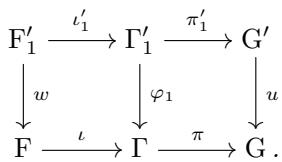
\includegraphics[keepaspectratio]{images/part002_e5b6b945.jpg}}

Then there exists a unique group homomorphism \(\psi : \Gamma_1' \to \Gamma'\) such that the diagram

\pandocbounded{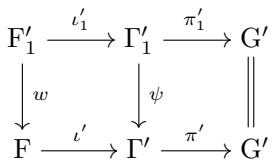
\includegraphics[keepaspectratio]{images/part002_7bcd6e81.jpg}}

commutes and \(\varphi_{1} = \varphi \circ \psi\) .

If the group homomorphism \(\psi : \Gamma_1' \to \Gamma'\) has the desired properties, then it satisfies the relations

\[
\psi (\gamma) = (\varphi \circ \psi (\gamma), \pi^ {\prime} \circ \psi (\gamma)) = (\varphi_ {1} (\gamma), \pi_ {1} ^ {\prime} (\gamma))
\]

for every \(\gamma \in \Gamma_1'\) . Conversely, the group homomorphism from \(\Gamma_1'\) to \(\Gamma \times G'\) defined by \(\gamma \mapsto (\varphi_1(\gamma), \pi_1'(\gamma))\) has values in the fiber product \(\Gamma \times_G G'\) because \(\pi \circ \varphi_1(\gamma) = u \circ \pi_1'(\gamma)\) for every \(\gamma \in \Gamma_1'\) .

COROLLARY 1. --- Let \(E_{1}\) and \(E_{2}\) be \(\tau\) -extensions of G by F, and let \(\psi\) be a morphism of \(\tau\) -extensions from \(E_{1}\) to \(E_{2}\) . Denote by \(\varphi_{1}\) (resp. \(\varphi_{2}\) ) the canonical homomorphism for \(u^{*}(\mathcal{E}_{1})\) (resp. \(u^{*}(\mathcal{E}_{2})\) ). Then there exists a unique morphism of \(\tau'\) -extensions from \(u^{*}(\mathcal{E}_{1})\) to \(u^{*}(\mathcal{E}_{2})\) , denoted by \(u^{*}(\psi)\) , such that \(\varphi_{2} \circ u^{*}(\psi) = \psi \circ \varphi_{1}\) .

It suffices to apply Proposition 1 to \(\psi \circ \varphi_{1}\) .

The class of the \(\tau^{\prime}\) -extension \(u^{*}(\mathcal{E})\) therefore depends only on the class of E. We also denote by \(u^{*}:\operatorname{Ex}_{\tau}(\mathrm{G},\mathrm{F})\to\operatorname{Ex}_{\tau^{\prime}}(\mathrm{G}^{\prime},\mathrm{F})\) the mapping that sends the class of a \(\tau\) -extension E to the class of the \(\tau^{\prime}\) -extension \(u^{*}(\mathcal{E})\) .

COROLLARY 2. --- Let \(u': G'' \to G'\) be a group homomorphism, and let \(\mathcal{E}\) be a \(\tau\) -extension of G by F. Set \(\tau'' = \tau' \circ u'\) , and denote by \(\varphi\) (resp. \(\varphi', \varphi''\) ) the canonical homomorphism associated with the \(\tau'\) -extension \(u^*(\mathcal{E})\) (resp. the \(\tau''\) -extension \(u'^*(u^*(\mathcal{E}))\) , the \(\tau''\) -extension \((u \circ u')^*(\mathcal{E})\) ). Then there exists a unique morphism \(\psi\) from the \(\tau''\) -extension \(u'^*(u^*(\mathcal{E}))\) to the \(\tau''\) -extension \((u \circ u')^*(\mathcal{E})\) such that \(\varphi'' \circ \psi = \varphi \circ \varphi'\) .

Example. --- Let H be a subgroup of G and \(j : H \to G\) the canonical injection. Then for every \(\tau\) -extension \(\mathcal{E} = (\Gamma, \iota, \pi)\) , the \(\tau \circ j\) -extension \(j^{*}(\mathcal{E})\) is isomorphic to \((\bar{\pi}^{1}(H), \iota', \pi')\) , where \(\iota' : F \to \bar{\pi}^{1}(H)\) (resp. \(\pi' : \bar{\pi}^{1}(H) \to H\) ) is the group homomorphism \(f \mapsto \iota(f)\) (resp. \(\gamma \mapsto \pi(\gamma)\) ). More generally, if the group homomorphism \(u : G' \to G\) is injective, then the canonical homomorphism \(\varphi\) is injective with image \(\bar{\pi}^{1}(u(G'))\) .

\subsection{\texorpdfstring{Direct Image of a \(\tau\)-Extension}{Direct Image of a \textbackslash tau-Extension}}

Let G be a group, let F and \(F'\) be abelian groups, let \(\tau\) (resp. \(\tau'\) ) be a group homomorphism from G to the automorphism group of F (resp. \(F'\) ), and let \(v: F \to F'\) be a group homomorphism such that

\[
v (\tau (g) \cdot f) = \tau^ {\prime} (g) \cdot v (f)\tag{3}
\]

for every \(g \in G\) and \(f \in F\) . Let \(\mathcal{E} = (\Gamma, \iota, \pi)\) be a \(\tau\) -extension of G by F. Let \(\widetilde{\Gamma}\) be the external semidirect product \(F' \times_{\tau' \circ \pi} \Gamma\) . We denote by \(\widetilde{\iota}: F' \to \widetilde{\Gamma}\) the homomorphism \(f \mapsto (f, e)\) and by \(\widetilde{p}: \widetilde{\Gamma} \to \Gamma\) the first projection. Let \(j: F \to \widetilde{\Gamma}\) be the mapping defined by \(f \mapsto (v(f), \iota(f)^{-1})\) . Since the image of \(\iota\) is contained in the kernel of \(\tau' \circ \pi\) , the mapping j is a group homomorphism; it is injective because \(\iota\) is injective. We have the relations

\[
\begin{array}{r l} (f ^ {\prime}, \gamma) j (f) (f ^ {\prime}, \gamma) ^ {- 1} & = (f ^ {\prime}, \gamma) (v (f), \iota (f) ^ {- 1}) (f ^ {\prime}, \gamma) ^ {- 1} \\ & = (\tau^ {\prime} (\pi (\gamma)) \cdot v (f), \iota (\tau (\pi (\gamma)) \cdot f) ^ {- 1}) \\ & = j (\tau (\pi (\gamma)) \cdot f) \end{array}\tag{4}
\]

for \(f \in F\) , \(\gamma \in \Gamma\) , and \(f' \in F'\) . Consequently, the image of j is a normal subgroup of \(\widetilde{\Gamma}\) . We denote by \(\Gamma'\) the quotient of \(\widetilde{\Gamma}\) by the image of j. We denote by \(\iota'\) the composition of the canonical surjection from \(\widetilde{\Gamma}\) to \(\Gamma'\) and \(\widetilde{\iota}\) . The kernel of the homomorphism \(\pi \circ \widetilde{p}\) is the product \(\mathrm{F}' \times \iota(\mathrm{F})\) , which contains the image of j. We define \(\pi' : \Gamma' \to G\) as the group homomorphism deduced from \(\pi \circ \widetilde{p}\) by passing to the quotient. Since \(\iota\) is injective, the intersection of \(j(\mathrm{F})\) and \(\widetilde{\iota}(\mathrm{F}')\) is reduced to the identity element of \(\widetilde{\Gamma}\) ; it follows that \(\iota'\) is injective. The mapping from \(F' \times F\) to \(F' \times \iota(\mathrm{F}) = \operatorname{Ker}(\pi \circ \widetilde{p})\) given by

\[
(f ^ {\prime}, f) \longmapsto (f ^ {\prime} v (f), \iota (f) ^ {- 1})
\]

is a group isomorphism. The image of \(\iota'\) therefore coincides with the kernel of \(\pi'\) . Since \(\pi\) and \(\widetilde{p}\) are surjective, so is \(\pi'\) . This proves that \(\mathcal{E}' = (\Gamma', \iota, \pi')\) is a \(\tau'\) -extension of \(G\) by \(F'\) ; we call it the direct image of \(\mathcal{E}\) by \(v\) and denote it by \(v_{*}(\mathcal{E})\) . The composition of the canonical surjection from \(\widetilde{\Gamma}\) to \(\Gamma'\) and the group homomorphism from \(\Gamma\) to \(\widetilde{\Gamma}\) given by \(\gamma \mapsto (1, \gamma)\) is a group homomorphism \(\varphi : \Gamma \to \Gamma'\) that we call canonical.

PROPOSITION 2. --- In the notation above, the following diagram commutes:

\begin{enumerate}
\def\labelenumi{(\arabic{enumi})}
\setcounter{enumi}{4}
\tightlist
\item
\end{enumerate}

\pandocbounded{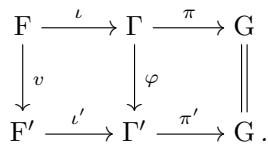
\includegraphics[keepaspectratio]{images/part002_f3abcdb3.jpg}}

Let \(\mathcal{E}_1' = (\Gamma_1', \iota_1', \pi_1')\) be a \(\tau'\) -extension of G by F', and let \(\varphi_1: \Gamma \to \Gamma_1'\) be a group homomorphism such that the following diagram commutes:

\pandocbounded{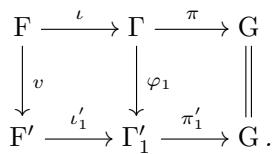
\includegraphics[keepaspectratio]{images/part002_c84edb93.jpg}}

Then there exists a unique morphism \(\psi\) of \(\tau'\) -extensions from \(v_{*}(\mathcal{E})\) to \(\mathcal{E}_1'\) such that we have \(\varphi_1 = \psi \circ \varphi\) .

The commutativity of the first diagram follows by construction. The existence and uniqueness of \(\psi\) follow from Lemma 3 below.

Lemma 3. --- Let \(G_{1}^{\prime}\) be a group, and let \(w: G \to G_{1}^{\prime}\) and \(\tau_{1}: G_{1}^{\prime} \to \operatorname{Aut}(F^{\prime})\) be group homomorphisms such that \(\tau^{\prime} = \tau_{1} \circ w\) . Let \(\mathcal{E}_{1}^{\prime} = (\Gamma_{1}^{\prime}, \iota_{1}^{\prime}, \pi_{1}^{\prime})\) be a \(\tau_{1}\) -extension of \(G_{1}^{\prime}\) by \(F^{\prime}\) , and let \(\varphi_{1}: \Gamma \to \Gamma_{1}^{\prime}\) be a group homomorphism such that the following diagram commutes:

\[
\begin{array}{c} \mathrm{F} \xrightarrow {\iota} \Gamma \xrightarrow {\pi} \mathrm{G} \\ \Biggl \downarrow_ {v} \qquad \qquad \Biggl \downarrow_ {\varphi_ {1}} \qquad \Biggl \downarrow_ {w} \\ \mathrm{F} ^ {\prime} \xrightarrow {\iota_ {1} ^ {\prime}} \Gamma_ {1} ^ {\prime} \xrightarrow {\pi_ {1} ^ {\prime}} \mathrm{G} _ {1} ^ {\prime}. \end{array}
\]

Then there exists a unique group homomorphism \(\psi : \Gamma' \to \Gamma'_1\) such that the diagram

\[
\begin{array}{c} \mathrm{F} ^ {\prime} \xrightarrow {\iota^ {\prime}} \Gamma^ {\prime} \xrightarrow {\pi^ {\prime}} \mathrm{G} \\ \Big \| \qquad \qquad \qquad \Big \downarrow_ {\psi} \qquad \Big \downarrow_ {w} \\ \mathrm{F} ^ {\prime} \xrightarrow {\iota_ {1} ^ {\prime}} \Gamma_ {1} ^ {\prime} \xrightarrow {\pi_ {1} ^ {\prime}} \mathrm{G} _ {1} ^ {\prime} \end{array}
\]

commutes and \(\varphi_{1} = \psi \circ \varphi\) .

For any \((f,\gamma)\in\mathrm{F}^{\prime}\times\Gamma\) , denote the class of \((f,\gamma)\) in \(\Gamma^{\prime}\) by \(\overline{(f,\gamma)}\) . If the group homomorphism \(\psi:\Gamma^{\prime}\to\Gamma_{1}^{\prime}\) has the desired properties, then it satisfies the relations

\[
\psi \big (\overline {{(f ^ {\prime} , \gamma)}} \big) = \psi (\iota^ {\prime} (f ^ {\prime}) \varphi (\gamma)) = \iota_ {1} ^ {\prime} (f ^ {\prime}) \varphi_ {1} (\gamma)
\]

for every \(f' \in \mathrm{F}'\) and \(\gamma \in \Gamma\) . Conversely, the mapping \(\tilde{\psi}\) from \(\mathrm{F}' \times_{\tau' \circ \pi} \Gamma\) to \(\Gamma_1'\) given by \((f, \gamma) \mapsto \iota_1'(f) \varphi_1(\gamma)\) is a group homomorphism. Indeed, we have the relations

\[
\begin{array}{r} \iota_ {1} ^ {\prime} (f) \varphi_ {1} (\gamma) \iota_ {1} ^ {\prime} (f ^ {\prime}) \varphi_ {1} (\gamma^ {\prime}) = \iota_ {1} ^ {\prime} (f \tau_ {1} (\pi_ {1} ^ {\prime} (\varphi_ {1} (\gamma))) \cdot f ^ {\prime}) \varphi_ {1} (\gamma \gamma^ {\prime}) \\ = \iota_ {1} ^ {\prime} (f \tau^ {\prime} (\pi (\gamma)) \cdot f ^ {\prime}) \varphi_ {1} (\gamma \gamma^ {\prime}) \end{array}
\]

for \(f, f' \in \mathrm{F}'\) and \(\gamma, \gamma' \in \Gamma\) . The kernel of \(\widetilde{\psi}\) contains the image of \(j\) because \(\iota_1'(v(f)) = \varphi_1(\iota(f))\) for \(f \in \mathrm{F}\) , and the morphism \(\psi\) deduced from \(\widetilde{\psi}\) by passing to the quotient has the desired properties.

Remark. --- Denote by \(\Sigma\) the species of structures of \(\tau'\) -extensions, and define \(\alpha\) -mappings to be mappings from \(\Gamma\) to a group \(\Gamma'\) underlying a \(\tau'\) -extension that are group homomorphisms and that make the following diagram commute:

\[
\begin{array}{c} \mathrm{F} \xrightarrow {\iota} \Gamma \xrightarrow {\pi} \mathrm{G} \\ \Big \downarrow v \qquad \qquad \Big \downarrow \varphi \\ \mathrm{F} ^ {\prime} \xrightarrow {\iota^ {\prime}} \Gamma^ {\prime} \xrightarrow {\pi^ {\prime}} \mathrm{G}. \end{array}\tag{6}
\]

Proposition 2 expresses that \(v_{*}(\mathcal{E})\) is a solution of the corresponding universal mapping problem (Set Theory, IV, §3, No.~1, p.~284).

COROLLARY 1. --- Let \(E_{1}\) and \(E_{2}\) be \(\tau\) -extensions of G by F, and let \(\psi\) be a morphism of \(\tau\) -extensions from \(E_{1}\) to \(E_{2}\) . Denote by \(\varphi_{1}\) (resp. \(\varphi_{2}\) ) the canonical homomorphism for \(v_{*}(\mathcal{E}_{1})\) (resp. \(v_{*}(\mathcal{E}_{2})\) ). Then there exists a unique morphism of \(\tau'\) -extensions from \(v_{*}(\mathcal{E}_{1})\) to \(v_{*}(\mathcal{E}_{2})\) , denoted by \(v_{*}(\psi)\) , such that \(\varphi_{2} \circ \psi = v_{*}(\psi) \circ \varphi_{1}\) .

It suffices to apply Proposition 2 to \(\varphi_{2} \circ \psi\) .

The class of the \(\tau^{\prime}\) -extension \(v_{*}(\mathcal{E})\) therefore depends only on the class of E. We also denote by \(v_{*}:\operatorname{Ex}_{\tau}(\mathrm{G},\mathrm{F})\to\operatorname{Ex}_{\tau^{\prime}}(\mathrm{G},\mathrm{F}^{\prime})\) the mapping that sends the class of a \(\tau\) -extension E to the class of the \(\tau^{\prime}\) -extension \(v_{*}(\mathcal{E})\) .

COROLLARY 2. --- We keep the notation of the proposition. Let F'' be an abelian group, and let \(\tau'' : G \to \text{Aut}(F'')\) and \(v': F' \to F''\) be group homomorphisms such that

\[
\tau^ {\prime \prime} (g) \cdot v ^ {\prime} (f) = v ^ {\prime} (\tau^ {\prime} (g) \cdot f)
\]

for \(g \in G\) and \(f \in F'\) . Let E be a \(\tau\) -extension of G by F, and denote by \(\varphi\) (resp. \(\varphi'\) , \(\varphi''\) ) the canonical homomorphism associated with \(v_{*}(\mathcal{E})\) (resp. \(v_{*}'(v_{*}(\mathcal{E}))\) , \((v' \circ v)_{*}(\mathcal{E})\) ). Then there exists a unique morphism \(\psi\) from the \(\tau''\) -extension \(v_{*}'(v_{*}(\mathcal{E}))\) of G by \(F''\) to the \(\tau''\) -extension \((v' \circ v)_{*}(\mathcal{E})\) such that \(\varphi'' = \psi \circ \varphi' \circ \varphi\) .

Examples. --- 1) Let \(j: \{1\} \to \mathrm{F}\) be the canonical injection. The semitrivial extension \(\mathcal{I}_{\tau}\) is isomorphic to \(j_{*}((\mathrm{G}, i, \mathrm{Id}_{\mathrm{G}}))\) , where \(i: \{e\} \to \mathrm{G}\) is the canonical injection. Let \(c: \mathrm{F} \to \mathrm{F}\) be the constant homomorphism \(f \mapsto 1\) , and let \(\mathcal{E}\) be a \(\tau\) -extension. The \(\tau\) -extension \(c_{*}(\mathcal{E})\) is also isomorphic to \(\mathcal{I}_{\tau}\) .

\begin{enumerate}
\def\labelenumi{\arabic{enumi})}
\setcounter{enumi}{1}
\tightlist
\item
  Let E be a subgroup of F stable under the action of G. Denote by \(F'\) the quotient of F by E, by \(v : F \to F'\) the canonical homomorphism, and by \(\tau' : G \to \text{Aut}(F')\) the action of G on \(F'\) characterized by
\end{enumerate}

\[
\tau^ {\prime} (g) \cdot v (f) = v (\tau (g) \cdot f)
\]

for \(g \in G\) and \(f \in F\) . Let \(\mathcal{E} = (\Gamma, \iota, \pi)\) be a \(\tau\) -extension of G by F. Then \(\iota(\mathrm{E})\) is a normal subgroup of \(\Gamma\) , and the \(\tau'\) -extension \(v_{*}(\mathcal{E})\) of G by \(F'\) is isomorphic to the extension \((\Gamma/\iota(\mathrm{E}), \bar{\iota}, \overline{\pi})\) , where \(\bar{\iota}\) and \(\overline{\pi}\) are the group homomorphisms deduced from \(\iota\) and \(\pi\) by passing to the quotients. By this isomorphism, the canonical homomorphism \(\varphi\) associated with \(v_{*}(\mathcal{E})\) corresponds to the canonical homomorphism from \(\Gamma\) to \(\Gamma/\iota(\mathrm{E})\) .

PROPOSITION 3. --- Let G and G' be groups, and let F and F' be abelian groups. Let \(\tau: \mathrm{G} \to \mathrm{Aut}(\mathrm{F})\) , \(\tau': \mathrm{G} \to \mathrm{Aut}(\mathrm{F}')\) , \(u: \mathrm{G}' \to \mathrm{G}\) , and \(v: \mathrm{F} \to \mathrm{F}'\) be group homomorphisms such that

\[
\tau^ {\prime} (g) \cdot v (f) = v (\tau (g) \cdot f)
\]

for \(g \in G\) and \(f \in F\) . We write \(\tau'' = \tau' \circ u\) . Let E be a \(\tau\) -extension of G by F. We denote by \(\varphi_u\) (resp. \(\varphi_v\) , \(\varphi'_u\) , \(\varphi'_v\) ) the canonical homomorphism corresponding to the \(\tau \circ u\) -extension \(u^*(\mathcal{E})\) (resp. to the \(\tau'\) -extension \(v_*(\mathcal{E})\) , to the \(\tau''\) -extensions \(u^*(v_*(\mathcal{E}))\) and \(v_*(u^*(\mathcal{E})))\) ). Then there exists a unique morphism \(\psi\) of \(\tau''\) -extensions from \(v_*(u^*(\mathcal{E}))\) to \(u^*(v_*(\mathcal{E}))\) such that \(\varphi_v \circ \varphi_u = \varphi'_u \circ \psi \circ \varphi'_v\) .

We denote the \(\tau \circ u\) -extension \(u^{*}(\mathcal{E})\) (resp. the \(\tau''\) -extension \(u^{*}(v_{*}(\mathcal{E}))\) ) by \((\Gamma_u, \iota_u, \pi_u)\) (resp. \((\Gamma_u', \iota_u', \pi_u')\) ). Applying Lemma 2 of VIII, p.~287 to \(\varphi_v \circ \varphi_u\) , we find that there exists a group homomorphism \(\psi_{1}:\Gamma_{u}\to\Gamma_{u}^{\prime}\) such that the diagram

\pandocbounded{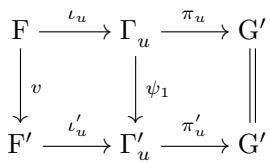
\includegraphics[keepaspectratio]{images/part002_ccea47d6.jpg}}

commutes and \(\varphi_{u}^{\prime}\circ\psi_{1}=\varphi_{v}\circ\varphi_{u}\) . The existence of \(\psi\) follows from Proposition 2 applied to \(\psi_{1}\) . Conversely, if \(\psi^{\prime}\) also has the desired properties, then we have \(\psi^{\prime}\circ\varphi_{v}^{\prime}=\psi_{1}\) by Lemma 2, so \(\psi^{\prime}=\psi\) (Proposition 2).

\subsection{\texorpdfstring{Group Law on the Classes of \(\tau\)-Extensions}{Group Law on the Classes of \textbackslash tau-Extensions}}

Let \(\mathrm{G}\) be a group, \(\mathrm{F}\) be an abelian group, and \(\tau : \mathrm{G} \to \mathrm{Aut}(\mathrm{F})\) be a group homomorphism. We denote by \(\delta : \mathrm{G} \to \mathrm{G} \times \mathrm{G}\) the diagonal mapping \(g \mapsto (g, g)\) and by \(m : \mathrm{F} \times \mathrm{F} \to \mathrm{F}\) the multiplication homomorphism \((f_1, f_2) \mapsto f_1 f_2\) . We denote by \(s : \mathrm{F} \to \mathrm{F}\) the group homomorphism given by \(f \mapsto f^{-1}\) . Let \(\mathcal{E}_1 = (\Gamma_1, \iota_1, \pi_1)\) and \(\mathcal{E}_2 = (\Gamma_2, \iota_2, \pi_2)\) be \(\tau\) -extensions of \(\mathrm{G}\) by \(\mathrm{F}\) . Since we have the relation

\[
m (((\tau \times \tau) \circ \delta) (g) \cdot (f _ {1}, f _ {2})) = \tau (g) \cdot m (f _ {1}, f _ {2})
\]

for every \(g \in G\) and all \(f_{1}, f_{2} \in F\) , the extension \(m_{*}(\delta^{*}(\mathcal{E}_{1} \times \mathcal{E}_{2}))\) is a \(\tau\) -extension; we call it the product of the \(\tau\) -extensions \(E_{1}\) and \(E_{2}\) and denote it by \(E_{1}E_{2}\) . The class of this extension depends only on the classes of the extensions \(E_{1}\) and \(E_{2}\) (VIII, p.~288, Corollary 1 and VIII, p.~291, Corollary 1). So this gives a law of composition on \(\operatorname{Ex}_{\tau}(\mathbf{G}, \mathbf{F})\) .

Remark. --- Let \(\mathcal{E}_{1}=(\Gamma_{1},\iota_{1},\pi_{1})\) and \(\mathcal{E}_{2}=(\Gamma_{2},\iota_{2},\pi_{2})\) be \(\tau\) -extensions of G by F. Let \(\mathcal{E}_{1}\mathcal{E}_{2}=(\Gamma,\iota,\pi)\) be the product of these extensions. Following the example of VIII, p.~289, the construction gives a surjective group homomorphism from the fiber product \(\Gamma_{1}\times_{G}\Gamma_{2}\) to \(\Gamma\) whose kernel is the image of the group homomorphism \(f\mapsto(\iota_{1}(f),\iota_{2}(f)^{-1})\) from F to \(\Gamma_{1}\times_{G}\Gamma_{2}\) .

PROPOSITION 4. --- The product of \(\tau\) -extensions endows the set \(\mathrm{Ex}_{\tau}(\mathrm{G},\mathrm{F})\) with the structure of an abelian group. Its identity element is the class of the semitrivial extension \(\mathcal{I}_{\tau}\) . The inverse of the class of a \(\tau\) -extension \(\mathcal{E}\) is the class of \(s_{*}(\mathcal{E})\) .

The associativity of the law follows from the commutativity of the diagrams

\pandocbounded{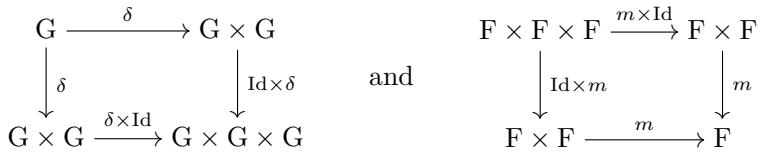
\includegraphics[keepaspectratio]{images/part002_39f17f00.jpg}}

and from Corollary 2 of VIII, p.~288; Corollary 2 of VIII, p.~291; and Proposition 3 of VIII, p.~292.

Let \(\Delta : \mathrm{F} \to \mathrm{F} \times \mathrm{F}\) be the diagonal mapping \(f \mapsto (f, f)\) . Let \(\mathcal{E} = (\Gamma, \iota, \pi)\) be a \(\tau\) -extension. Let \(\widetilde{\Delta}: \Gamma \to \Gamma \times_{\mathrm{G}} \Gamma\) be the group homomorphism given by \(\gamma \mapsto (\gamma, \gamma)\) . The following diagram commutes:

\pandocbounded{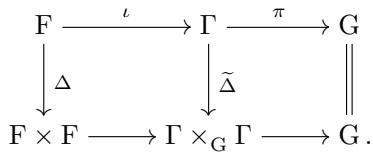
\includegraphics[keepaspectratio]{images/part002_db57599b.jpg}}

By Proposition 2 of VIII, p.~290, it follows that the \((\tau \times \tau) \circ \delta\) -extension \(\delta^{*}(\mathcal{E} \times \mathcal{E})\) is isomorphic to \(\Delta_{*}(\mathcal{E})\) .

Denote by \(c: F \to F\) the constant homomorphism \(f \mapsto 1\) . by Example 1 of VIII, p.~292, the fact that \(\mathcal{I}_{\tau}\) is an identity element for this law of composition follows from the isomorphism from \(\delta^{*}(\mathcal{E} \times \mathcal{E})\) to \(\Delta_{*}(\mathcal{E})\) and the commutative diagram

\pandocbounded{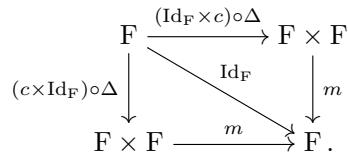
\includegraphics[keepaspectratio]{images/part002_761b87f2.jpg}}

The last assertion follows from the commutative diagram

\[
\begin{array}{c} \mathrm{F} \xrightarrow {(\mathrm{Id} _ {\mathrm{F}} \times s) \circ \Delta} \mathrm{F} \times \mathrm{F} \\ (s \times \mathrm{Id} _ {\mathrm{F}}) \circ \Delta \Biggl \downarrow \qquad \qquad \qquad \qquad \qquad \qquad \qquad \qquad \qquad \qquad \qquad \qquad \qquad \qquad \qquad \qquad \qquad \qquad \qquad \qquad \qquad \qquad \qquad \qquad \qquad \qquad \qquad \qquad \qquad \qquad \qquad \qquad \qquad \qquad \\ \mathrm{F} \times \mathrm{F} \xrightarrow {m} \mathrm{F}. \end{array}
\]

Let \(\mathcal{E}_1 = (\Gamma_1,\iota_1,\pi_1)\) and \(\mathcal{E}_2 = (\Gamma_2,\iota_2,\pi_2)\) be \(\tau\) -extensions. The group isomorphism \(\Gamma_1\times \Gamma_2\to \Gamma_2\times \Gamma_1\) given by \((\gamma_{1},\gamma_{2})\mapsto (\gamma_{2},\gamma_{1})\) restricts to a group isomorphism \(\sigma :\Gamma_1\times_\mathrm{G}\Gamma_2\to \Gamma_2\times_\mathrm{G}\Gamma_1\) . Because of the relations

\[
\sigma (\iota_ {1} (f), \iota_ {2} (f) ^ {- 1}) = (\iota_ {2} (f ^ {- 1}), \iota_ {1} (f ^ {- 1}) ^ {- 1})
\]

for \(f \in F\) , the group homomorphism \(\sigma\) induces, by passing to the quotients, a morphism of \(\tau\) -extensions from \(E_{1}E_{2}\) to \(E_{2}E_{1}\) . So the law of composition is commutative.

PROPOSITION 5. --- a) Let G and G' be groups, and let F be an abelian group. Let \(\tau: \mathrm{G} \to \operatorname{Aut}(\mathrm{F})\) and \(u: \mathrm{G}' \to \mathrm{G}\) be group homomorphisms. The mapping \(u^*: \operatorname{Ex}_{\tau}(\mathrm{G}, \mathrm{F}) \to \operatorname{Ex}_{\tau \circ u}(\mathrm{G}', \mathrm{F})\) is a group homomorphism.

\begin{enumerate}
\def\labelenumi{\alph{enumi})}
\setcounter{enumi}{1}
\tightlist
\item
  Let G be a group, and let F and \(F'\) be abelian groups. Let \(\tau: G \to \text{Aut}(F)\) , \(\tau': G \to \text{Aut}(F')\) , and \(v: F \to F'\) be group homomorphisms such that
\end{enumerate}

\[
\tau^ {\prime} (g) \cdot v (f) = v (\tau (g) \cdot f)
\]

for \(g \in \mathrm{G}\) and \(f \in \mathrm{F}\) . The mapping \(v_{*} : \operatorname{Ex}_{\tau}(\mathrm{G}, \mathrm{F}) \to \operatorname{Ex}_{\tau'}(\mathrm{G}, \mathrm{F}')\) is a group homomorphism.

This follows from the commutativity of the diagrams

\[
\begin{array}{l} \mathrm{G} ^ {\prime} \xrightarrow {\delta} \mathrm{G} ^ {\prime} \times \mathrm{G} ^ {\prime} \\ \Biggl \downarrow_ {u} \qquad \Biggl \downarrow_ {u \times u} \\ \mathrm{G} \xrightarrow {\delta} \mathrm{G} \times \mathrm{G} \end{array} \qquad \text {and} \qquad \begin{array}{l} \mathrm{F} \times \mathrm{F} \xrightarrow {m} \mathrm{F} \\ \Biggl \downarrow_ {v \times v} \qquad \Biggl \downarrow_ {v} \\ \mathrm{F} ^ {\prime} \times \mathrm{F} ^ {\prime} \xrightarrow {m} \mathrm{F} ^ {\prime}. \end{array}
\]

\subsection{Cohomological Description}

Let G be a group, let F be an abelian group, and let \(\tau: G \to \text{Aut}(F)\) be a group homomorphism. For any \(g \in G\) and \(f \in F\) , we also write \(^{g}f\) for \(\tau(g) \cdot f\) . A 2-cocycle of G with values in F is a mapping \(c: G \times G \to F\) such that for every \((g_{1}, g_{2}, g_{3}) \in G \times G \times G\) , we have

\[
{ } ^ { g _ { 1 } } c ( g _ { 2 } , g _ { 3 } ) c ( g _ { 1 } , g _ { 2 } g _ { 3 } ) = c ( g _ { 1 } , g _ { 2 } ) c ( g _ { 1 } g _ { 2 } , g _ { 3 } ) .\tag{7}
\]

Since F is commutative, the set of 2-cocycles is a subgroup of the group of mappings from \(G \times G\) to F; we denote it by \(Z^{2}(G,F)\) . We denote the group of mappings from G to F by \(C^{1}(G,F)\) . For every \(h \in C^{1}(G,F)\) and \((g_{1}, g_{2}) \in G \times G\) , set

\[
(\partial h) (g _ {1}, g _ {2}) = ^ {g _ {1}} h (g _ {2}) h (g _ {1} g _ {2}) ^ {- 1} h (g _ {1}).\tag{8}
\]

A simple calculation shows that the mapping \(\partial h: G \times G \to F\) is a 2-cocycle. The mapping \(\partial: C^{1}(G, F) \to Z^{2}(G, F)\) is a group homomorphism. For any \(h \in C^{1}(G, F)\) , the 2-cocycle \(\partial h\) is called a 2-coboundary. The group

\(Z^{2}(G,F)/\partial(C^{1}(G,F))\) is denoted by \(H^{2}(G,F)\) and is called the second cohomology group of G with coefficients in F.

*The notation above agrees with that of X, §6, n° 8, p.~112 concerning group cohomology.*

Let \(\mathcal{E} = (\Gamma, \iota, \pi)\) be a \(\tau\) -extension. Let \(\sigma\) be a section of the surjective mapping \(\pi\) (Set Theory, II, §3, No.~8, p.~86), that is, a mapping from G to \(\Gamma\) such that \(\pi(\sigma(g)) = g\) for every \(g\) in G. For every \(g_1, g_2 \in G\) , \(\sigma(g_1)\sigma(g_2)\sigma(g_1g_2)^{-1}\) belongs to \(\mathrm{Ker}(\pi)\) , so that there exists a unique mapping \(c_\sigma: G \times G \to F\) such that

\[
\iota (c _ {\sigma} (g _ {1}, g _ {2})) = \sigma (g _ {1}) \sigma (g _ {2}) \sigma (g _ {1} g _ {2}) ^ {- 1}\tag{9}
\]

for all \(g_{1}, g_{2} \in G\) . The mapping \(c_{\sigma}\) is constant with value 1 if and only if \(\sigma\) is a group homomorphism.

PROPOSITION 6. --- The mapping \(c_{\sigma}\) is an element of the group \(Z^{2}(G,F)\) , and its class in the cohomology group \(H^{2}(G,F)\) depends only on the class of the \(\tau\) -extension E.

We say that the mapping \(c_{\sigma}\) is the 2-cocycle associated with \(\sigma\) and that its cohomology class in \(\mathrm{H}^2 (\mathrm{G},\mathrm{F})\) is the cohomology class of the \(\tau\) -extension \(\mathcal{E}\) .

Let us first verify that \(c_{\sigma}\) satisfies the cocycle condition. Let \(g_{1}, g_{2}\) , and \(g_{3}\) be elements of G. Using formula (1) of VIII, p.~285 and (9), we obtain the relations

\[
\begin{array}{r l} & {\iota (g _ {1} c _ {\sigma} (g _ {2}, g _ {3}) c _ {\sigma} (g _ {1}, g _ {2} g _ {3}))} \\ & {\quad = \sigma (g _ {1}) \sigma (g _ {2}) \sigma (g _ {3}) \sigma (g _ {2} g _ {3}) ^ {- 1} \sigma (g _ {1}) ^ {- 1} \sigma (g _ {1}) \sigma (g _ {2} g _ {3}) \sigma (g _ {1} g _ {2} g _ {3}) ^ {- 1}} \\ & {\quad = \sigma (g _ {1}) \sigma (g _ {2}) \sigma (g _ {3}) \sigma (g _ {1} g _ {2} g _ {3}) ^ {- 1}} \end{array}
\]

and

\[
\begin{array}{r l} & {\iota (c _ {\sigma} (g _ {1}, g _ {2}) c _ {\sigma} (g _ {1} g _ {2}, g _ {3}))} \\ & {\qquad = \sigma (g _ {1}) \sigma (g _ {2}) \sigma (g _ {1} g _ {2}) ^ {- 1} \sigma (g _ {1} g _ {2}) \sigma (g _ {3}) \sigma (g _ {1} g _ {2} g _ {3}) ^ {- 1}} \\ & {\qquad = \sigma (g _ {1}) \sigma (g _ {2}) \sigma (g _ {3}) \sigma (g _ {1} g _ {2} g _ {3}) ^ {- 1}.} \end{array}
\]

The mapping \(c_{\sigma}\) is therefore an element of \(\mathbf{Z}^2 (\mathrm{G},\mathrm{F})\) .

Let us now prove that the image of \(c_{\sigma}\) in \(\mathrm{H}^{2}(\mathrm{G},\mathrm{F})\) is independent of the chosen section \(\sigma\) . Let \(\sigma\) and \(\sigma'\) be such sections. For every element g of G, there exists a unique element \(a_{g}\) of F such that \(\sigma'(g) = \iota(a_{g})\sigma(g)\) . Let \(g_{1}\) and \(g_{2}\) be elements of G. Using the definition (9), we obtain the equalities

\[
\begin{array}{r l} & {\iota (c _ {\sigma^ {\prime}} (g _ {1}, g _ {2})) = \sigma^ {\prime} (g _ {1}) \sigma^ {\prime} (g _ {2}) \sigma^ {\prime} (g _ {1} g _ {2}) ^ {- 1}} \\ & {\qquad = \iota (a _ {g _ {1}}) \sigma (g _ {1}) \iota (a _ {g _ {2}}) \sigma (g _ {2}) \sigma (g _ {1} g _ {2}) ^ {- 1} \iota (a _ {g _ {1} g _ {2}}) ^ {- 1}} \\ & {\qquad = \iota (a _ {g _ {1}}) \iota (^ {g _ {1}} a _ {g _ {2}}) \iota (c _ {\sigma} (g _ {1}, g _ {2})) \iota (a _ {g _ {1} g _ {2}}) ^ {- 1}.} \end{array}\tag{10}
\]

Since the group F is commutative, we have the relations

\[
c _ {\sigma^ {\prime}} (g _ {1}, g _ {2}) c _ {\sigma} (g _ {1}, g _ {2}) ^ {- 1} = (^ {g _ {1}} a _ {g _ {2}}) a _ {g _ {1} g _ {2}} ^ {- 1} a _ {g _ {1}} = (\partial a) (g _ {1}, g _ {2}),\tag{11}
\]

as follows from (8). This proves that the classes of \(c_{\sigma'}\) and \(c_{\sigma}\) in \(\mathrm{H}^2(\mathrm{G},\mathrm{F})\) coincide.

Finally, let \(\mathcal{E} = (\Gamma, \iota, \pi)\) and \(\mathcal{E}' = (\Gamma', \iota', \pi')\) be isomorphic \(\tau\) -extensions, let \(u: \mathcal{E} \to \mathcal{E}'\) be a morphism of \(\tau\) -extensions, and let \(\sigma\) be a section of the mapping \(\pi\) . The mapping \(u \circ \sigma\) is a section of the mapping \(\pi'\) , and we have \(c_{\sigma} = c_{u \circ \sigma}\) . The class of \(c_{\sigma}\) in \(\mathrm{H}^2(\mathrm{G}, \mathrm{F})\) therefore depends only on the class of \(\mathcal{E}\) in \(\mathrm{Ex}_{\tau}(\mathrm{G}, \mathrm{F})\) .

We denote by \(\Theta_{\tau}: \operatorname{Ex}_{\tau}(\mathrm{G},\mathrm{F}) \to \mathrm{H}^{2}(\mathrm{G},\mathrm{F})\) , or more simply \(\Theta\) , the mapping that sends the class of a \(\tau\) -extension \((\Gamma,\iota,\pi)\) to the class of the 2-cocycle \(c_{\sigma}\) , where \(\sigma\) is a section of the surjection \(\pi\) .

THEOREM 1. --- The mapping \(\Theta\) is a group isomorphism from \(\operatorname{Ex}_{\tau}(\mathrm{G},\mathrm{F})\) to \(\mathrm{H}^2 (\mathrm{G},\mathrm{F})\) .

Let us first prove that \(\Theta\) is a group homomorphism. Let \(\mathcal{E} = (\Gamma, \iota, \pi)\) and \(\mathcal{E}' = (\Gamma', \iota', \pi')\) be \(\tau\) -extensions, and let \(\sigma\) (resp. \(\sigma'\) ) be a section of the mapping \(\pi\) (resp. \(\pi'\) ). We denote by \(\mathcal{E}\mathcal{E}' = (\Gamma'', \iota'', \pi'')\) the product of the \(\tau\) -extensions E and \(E'\) . We denote by \([\gamma, \gamma']\) the image in \(\Gamma''\) of an element \((\gamma, \gamma')\) of \(\Gamma \times_{G} \Gamma'\) by the surjective homomorphism from the remark of VIII, p.~293. The mapping from G to \(\Gamma''\) that sends an element g to \([\sigma(g), \sigma'(g)]\) is a section \(\sigma''\) of the mapping \(\pi''\) . Let \(g_1\) and \(g_2\) be elements of G. We have the relations

\[
\begin{array}{r l} & {\iota^ {\prime \prime} (c _ {\sigma^ {\prime \prime}} (g _ {1}, g _ {2})) = \sigma^ {\prime \prime} (g _ {1}) \sigma^ {\prime \prime} (g _ {2}) \sigma^ {\prime \prime} (g _ {1} g _ {2}) ^ {- 1}} \\ & {\qquad = [ \iota (c _ {\sigma} (g _ {1}, g _ {2})), \iota^ {\prime} (c _ {\sigma^ {\prime}} (g _ {1}, g _ {2}) ]} \\ & {\qquad = \iota^ {\prime \prime} (c _ {\sigma} (g _ {1}, g _ {2}) c _ {\sigma^ {\prime}} (g _ {1}, g _ {2})).} \end{array}
\]

We therefore have \(c_{\sigma''}(g_1, g_2) = c_\sigma(g_1, g_2)c_{\sigma'}(g_1, g_2)\) .

Let us prove that the mapping \(\Theta\) is injective. Let \(\mathcal{E} = (\Gamma, \iota, \pi)\) be a \(\tau\) -extension, and let \(\sigma\) be a section of the mapping \(\pi\) such that the image of \(c_{\sigma}\) in \(\mathrm{H}^{2}(\mathrm{G}, \mathrm{F})\) is trivial. There exists a mapping \(a : G \to F\) such that

\[
c _ {\sigma} (g _ {1}, g _ {2}) = (^ {g _ {1}} a (g _ {2})) a (g _ {1} g _ {2}) ^ {- 1} a (g _ {1})
\]

for all \(g_{1}, g_{2} \in G\) . We then define \(\sigma' : G \to \Gamma\) by

\[
\sigma^ {\prime} (g) = \iota (a (g) ^ {- 1}) \sigma (g)
\]

for \(g \in G\) . Using (11), we obtain that \(c_{\sigma'}\) is constant with value 1; consequently, \(\sigma'\) is a group homomorphism, which proves that the \(\tau\) -extension E is semitrivial (I, §6, No.~1, p.~67, Proposition 4).

Let us prove that the mapping \(\Theta\) is surjective. Let c be an element of \(Z^{2}(G,F)\) . We endow the set \(\Gamma = F \times G\) with the following law of composition:

\[
(f _ {1}, g _ {1}) (f _ {2}, g _ {2}) = \left(f _ {1} (^ {g _ {1}} f _ {2}) c (g _ {1}, g _ {2}), g _ {1} g _ {2}\right)\tag{12}
\]

for all \(f_{1}, f_{2} \in F\) and \(g_{1}, g_{2} \in G\) . We have the relations

\[
\begin{array}{r l} (f _ {1}, g _ {1}) ((f _ {2}, g _ {2}) (f _ {3}, g _ {3})) & = (f _ {1}, g _ {1}) \big (f _ {2} (^ {g _ {2}} f _ {3}) c (g _ {2}, g _ {3}), g _ {2} g _ {3} \big) \\ & = \big (f _ {1} (^ {g _ {1}} f _ {2}) (^ {g _ {1} g _ {2}} f _ {3}) (^ {g _ {1}} c (g _ {2}, g _ {3})) c (g _ {1}, g _ {2} g _ {3}), g _ {1} g _ {2} g _ {3} \big) \end{array}
\]

and

\[
\begin{array}{c} ((f _ {1}, g _ {1}) (f _ {2}, g _ {2}))   (f _ {3}, g _ {3}) = \big (f _ {1} (^ {g _ {1}} f _ {2}) c (g _ {1}, g _ {2}), g _ {1} g _ {2} \big) (f _ {3}, g _ {3}) \\ = \big (f _ {1} (^ {g _ {1}} f _ {2}) (^ {g _ {1} g _ {2}} f _ {3}) c (g _ {1}, g _ {2}) c (g _ {1} g _ {2}, g _ {3}), g _ {1} g _ {2} g _ {3} \big) \end{array}
\]

for all \(f_{1}, f_{2}, f_{3} \in F\) and \(g_{1}, g_{2}, g_{3} \in G\) . It follows that this law is associative because c is a 2-cocycle. For every \((f, g) \in \Gamma\) , we have

\[
(f, g) (c (e, e) ^ {- 1}, e) = (f (^ {g} c (e, e) ^ {- 1}) c (g, e), g).
\]

Now, it follows from the definition of a 2-cocycle that \(c(g, e) = {}^g c(e, e)\) , from which we deduce that \((f, g)(c(e, e)^{-1}, e) = (f, g)\) . We prove likewise that

\[
(c (e, e) ^ {- 1}, e) (f, g) = (f c (e, e) ^ {- 1} c (e, g), g) = (f, g).
\]

The law of composition defined by (12) therefore has identity element \((c(e,e)^{-1},e)\) , and every element \((f,g)\) of \(\Gamma\) is invertible, with inverse

\[
\left(^ {g ^ {- 1}} (f ^ {- 1} c (e, e) ^ {- 1} c (g, g ^ {- 1}) ^ {- 1}), g ^ {- 1}\right).
\]

So we have endowed \(\Gamma\) with a group structure. Let us denote by \(\iota: F \to G\) the mapping that sends f to \((c(e, e)^{-1}f, e)\) , by \(\pi: \Gamma \to G\) the second projection, and by \(\sigma\) the mapping \(g \mapsto (1, g)\) . The mappings \(\iota\) and \(\pi\) are group homomorphisms, so the triple \(\mathcal{E} = (\Gamma, \iota, \pi)\) is a \(\tau\) -extension, \(\sigma\) is a section of the mapping \(\pi\) , and the associated cocycle \(c_{\sigma}\) is equal to c because

\[
\begin{array}{c} \sigma (g _ {1}) \sigma (g _ {2}) \sigma (g _ {1} g _ {2}) ^ {- 1} = (1, g _ {1}) (1, g _ {2}) (1, g _ {1} g _ {2}) ^ {- 1} = (c (g _ {1}, g _ {2}), g _ {1} g _ {2}) (1, g _ {1} g _ {2}) ^ {- 1} \\ = (c (g _ {1}, g _ {2}) c (e, g _ {1} g _ {2}) ^ {- 1}, e) = (c (e, e) ^ {- 1} c (g _ {1}, g _ {2}), e) \end{array}
\]

for \(g_{1}, g_{2} \in G\) .

Remark. --- Let G be a group, let F and \(F'\) be abelian groups, let \(\tau\) (resp. \(\tau'\) ) be a group homomorphism from G to the automorphism group of F (resp. \(F'\) ), and let \(v : F \to F'\) be a group morphism such that

\[
v (\tau (g) \cdot f) = \tau^ {\prime} (g) \cdot v (f)\tag{13}
\]

for \(g \in G\) and \(f \in F\) . Let \(\alpha\) be an element of \(\operatorname{Ex}_{\tau}(\mathrm{G}, \mathrm{F})\) . If the cocycle c represents \(\Theta(\alpha)\) , then \(v \circ c\) represents \(\Theta(v_{*}(\alpha)) \in \mathrm{H}^{2}(\mathrm{G}, \mathrm{F}')\) .

\subsection{Restriction and Corestriction}

Let G and \(G'\) be groups, F be an abelian group, and \(\tau\) be a homomorphism from G to the automorphism group of F. Let \(u: G' \to G\) be a group homomorphism. We write \(\tau' = \tau \circ u\) .

If \(\psi : \mathrm{G} \times \mathrm{G} \to \mathrm{F}\) is a 2-cocycle of \(\mathrm{G}\) with values in \(\mathrm{F}\) , then the mapping \(\psi \circ (u \times u)\) from \(\mathrm{G}' \times \mathrm{G}'\) to \(\mathrm{F}\) given by \((g_1, g_2) \mapsto \psi(u(g_1), u(g_2))\) is a 2-cocycle of \(\mathrm{G}'\) with values in \(\mathrm{F}\) , and the mapping \(\psi \mapsto \psi \circ (u \times u)\) from \(\mathrm{Z}^2(\mathrm{G}, \mathrm{F})\) to \(\mathrm{Z}^2(\mathrm{G}', \mathrm{F})\) induces a group homomorphism \(u^*: \mathrm{H}^2(\mathrm{G}, \mathrm{F}) \to \mathrm{H}^2(\mathrm{G}', \mathrm{F})\) . For any \(\lambda \in \mathrm{H}^2(\mathrm{G}, \mathrm{F})\) , the element \(u^*(\lambda)\) is called the inverse image of \(\lambda\) by \(u\) . When \(\mathrm{G}'\) is a subgroup of \(\mathrm{G}\) and \(u: \mathrm{G}' \to \mathrm{G}\) is the canonical injection, the homomorphism \(u^*\) is called the restriction homomorphism from \(\mathrm{G}\) to \(\mathrm{G}'\) ; we denote it by \(\operatorname{Res}_{\mathrm{G}'}^{\mathrm{G}}\) . When \(\mathrm{G}\) is a quotient of \(\mathrm{G}'\) and \(u: \mathrm{G}' \to \mathrm{G}\) is the canonical surjection, the homomorphism \(u^*\) is called the inflation homomorphism from \(\mathrm{G}\) to \(\mathrm{G}'\) .

PROPOSITION 7. --- In the notation from above, the following diagram commutes:

\[
\begin{array}{c} \operatorname{Ex} _ {\tau} (\mathrm{G}, \mathrm{F}) \xrightarrow {u ^ {*}} \operatorname{Ex} _ {\tau} (\mathrm{G} ^ {\prime}, \mathrm{F}) \\ \Biggl \downarrow \Theta_ {\tau} \qquad \qquad \qquad \Biggl \downarrow \Theta_ {\tau^ {\prime}} \\ \operatorname{H} ^ {2} (\mathrm{G}, \mathrm{F}) \xrightarrow {u ^ {*}} \operatorname{H} ^ {2} (\mathrm{G} ^ {\prime}, \mathrm{F})  . \end{array}
\]

Let H be a subgroup of G of finite index. Let s be a section of the canonical surjection from G to \(H\backslash G\). We denote by \((g,x)\mapsto x\cdot g\) the right action of G on \(H\backslash G\) induced by the right action of G on itself by multiplication. Note that for every \(x\in H\backslash G\) and \(g\in G\) , the element \(s(x)gs(x\cdot g)^{-1}\) belongs to H. For any mapping \(c: \mathrm{H} \times \mathrm{H} \to \mathrm{F}\) , we can therefore define a mapping \(\widetilde{c}_s: \mathrm{G} \times \mathrm{G} \to \mathrm{F}\) by the relation

\[
\widetilde {c} _ {s} (g _ {1}, g _ {2}) = \prod_ {x \in \mathrm{H} \backslash \mathrm{G}} ^ {s (x) ^ {- 1}} c \bigl (s (x) g _ {1} s (x \cdot g _ {1}) ^ {- 1}, s (x \cdot g _ {1}) g _ {2} s (x \cdot g _ {1} g _ {2}) ^ {- 1} \bigr)
\]

for \(g_{1}, g_{2} \in G\) . The mapping \(c \mapsto \widetilde{c}_{s}\) is a group homomorphism from \(F^{H \times H}\) to \(F^{G \times G}\) .

Lemma 4. --- If \(c: \mathrm{H} \times \mathrm{H} \to \mathrm{F}\) is a 2-cocycle of H with values in F, then \(\widetilde{c}_s\) is a 2-cocycle of G with values in F.

Let \(g_1, g_2\) , and \(g_3\) be elements of G. For every \(i \in \{1, 2, 3\}\) , we define a mapping \(h_i: \mathrm{H} \backslash \mathrm{G} \to \mathrm{H}\) by the relation

\[
h _ {i} (x) = s \left(x \cdot g _ {1} \dots g _ {i - 1}\right) g _ {i} s \left(x \cdot g _ {1} \dots g _ {i}\right) ^ {- 1}
\]

for \(x\in \mathrm{H}\backslash \mathrm{G}\) . Note that

\[
\begin{array}{l} {h _ {1} (x) h _ {2} (x) = s (x) g _ {1} g _ {2} s (x \cdot g _ {1} g _ {2}) ^ {- 1}} \\ {h _ {2} (x) h _ {3} (x) = s (x \cdot g _ {1}) g _ {2} g _ {3} s (x \cdot g _ {1} g _ {2} g _ {3}) ^ {- 1}} \end{array}
\]

for \(x \in \mathrm{H} \backslash \mathrm{G}\) . We then have the relations

\[
\begin{array}{r l} & ^ {g _ {1}} \widetilde {c} _ {s} (g _ {2}, g _ {3}) \widetilde {c} _ {s} (g _ {1} g _ {2}, g _ {3}) ^ {- 1} \widetilde {c} _ {s} (g _ {1}, g _ {2} g _ {3}) \widetilde {c} _ {s} (g _ {1}, g _ {2}) ^ {- 1} \\ & \quad = \prod_ {x \in \mathrm{H} \backslash \mathrm{G}} ^ {g _ {1} s (x) ^ {- 1}} c \big (s (x) g _ {2} s (x \cdot g _ {2}) ^ {- 1}, s (x \cdot g _ {2}) g _ {3} s (x \cdot g _ {2} g _ {3}) ^ {- 1} \big) \\ & \qquad \times \prod_ {x \in \mathrm{H} \backslash \mathrm{G}} ^ {s (x) ^ {- 1}} \Big (c (h _ {1} (x) h _ {2} (x), h _ {3} (x)) ^ {- 1} \\ & \qquad \qquad \qquad \qquad \times c (h _ {1} (x), h _ {2} (x) h _ {3} (x))   c (h _ {1} (x), h _ {2} (x)) ^ {- 1} \Big) \\ & = \prod_ {x \in \mathrm{H} \backslash \mathrm{G}} ^ {s (x \cdot g _ {1} ^ {- 1}) ^ {- 1} h _ {1} (x \cdot g _ {1} ^ {- 1})} c (h _ {2} (x \cdot g _ {1} ^ {- 1}), h _ {3} (x \cdot g _ {1} ^ {- 1})) \\ & \qquad \times \prod_ {x \in \mathrm{H} \backslash \mathrm{G}} ^ {s (x) ^ {- 1} h _ {1} (x)} c (h _ {2} (x), h _ {3} (x)) ^ {- 1} \\ & = 1, \end{array}
\]

where the second equality follows from the fact that c is a 2-cocycle.

Lemma 5. --- If \(c\) is a 2-coboundary, then so is \(\widetilde{c}_s\) .

Let \(t: \mathrm{H} \to \mathrm{F}\) be a mapping such that \(c = \partial t\) . Let \(\widetilde{t}_s: \mathrm{G} \to \mathrm{F}\) be the mapping defined by

\[
\widetilde {t} _ {s} (g) = \prod_ {x \in \mathrm{H} \backslash \mathrm{G}} ^ {s (x) ^ {- 1}} t (s (x) g s (x \cdot g) ^ {- 1})
\]

for \(g \in G\) . It suffices to prove that \(\widetilde{c}_{s} = \partial\widetilde{t}_{s}\) , which follows from the relations

\[
\begin{array}{l} \widetilde {c} _ {s} (g _ {1}, g _ {2}) = \prod_ {x \in \mathrm{H} \backslash \mathrm{G}} ^ {s (x) ^ {- 1} s (x) g _ {1} s (x \cdot g _ {1}) ^ {- 1}} t (s (x \cdot g _ {1}) g _ {2} s (x \cdot g _ {1} g _ {2}) ^ {- 1}) \\ \qquad \times \prod_ {x \in \mathrm{H} \backslash \mathrm{G}} ^ {s (x) ^ {- 1}} \big (t (s (x) g _ {1} g _ {2} s (x \cdot g _ {1} g _ {2}) ^ {- 1}) ^ {- 1} t (s (x) g _ {1} s (x \cdot g _ {1}) ^ {- 1}) \big) \\ = \partial \widetilde {t} _ {s} (g _ {1}, g _ {2}) \end{array}
\]

for \(g_{1}, g_{2} \in G\) .

Lemma 6. --- Let c be a 2-cocycle of H with values in F. The image of \(\widetilde{c}_{s}\) in the group \(\mathrm{H}^{2}(\mathrm{G},\mathrm{F})\) does not depend on the choice of the section s.

Let \(s'\) be a section of the canonical surjection from G to \(H\backslash G\). Let \(h: \mathrm{H} \backslash \mathrm{G} \to \mathrm{H}\) be the mapping characterized by the relation

\[
s ^ {\prime} (x) = h (x) s (x)
\]

for \(x \in H \backslash G\) . The 2-cocycle \(\widetilde{c}_{s'}\) is then given by the relations

\[
\begin{array}{l} \widetilde {c} _ {s ^ {\prime}} (g _ {1}, g _ {2}) \\ = \prod_ {x \in \mathrm{H} \backslash \mathrm{G}} ^ {s (x) ^ {- 1} h (x) ^ {- 1}} c \big (h (x) s (x) g _ {1} s ^ {\prime} (x \cdot g _ {1}) ^ {- 1}, s ^ {\prime} (x \cdot g _ {1}) g _ {2} s ^ {\prime} (x \cdot g _ {1} g _ {2}) ^ {- 1} \big) \\ = \prod_ {x \in \mathrm{H} \backslash \mathrm{G}} ^ {s (x) ^ {- 1}} c \big (s (x) g _ {1} s (x \cdot g _ {1}) ^ {- 1} h (x \cdot g _ {1}) ^ {- 1}, h (x \cdot g _ {1}) s (x \cdot g _ {1}) g _ {2} s ^ {\prime} (x \cdot g _ {1} g _ {2}) ^ {- 1} \big) \\ \qquad \times \prod_ {x \in \mathrm{H} \backslash \mathrm{G}} ^ {s (x) ^ {- 1}} \Big (c \big (h (x) ^ {- 1}, s ^ {\prime} (x) g _ {1} g _ {2} s ^ {\prime} (x \cdot g _ {1} g _ {2}) ^ {- 1} \big) ^ {- 1} \\ \qquad \qquad \qquad \qquad \qquad \qquad \qquad \qquad \qquad \qquad \qquad \qquad \qquad \qquad \qquad \qquad \qquad \qquad \qquad \qquad \qquad \qquad \qquad \qquad \qquad \qquad \qquad \qquad \qquad \qquad \qquad \qquad \qquad \qquad \\ = \prod_ {x \in \mathrm{H} \backslash \mathrm{G}} ^ {g _ {1} s (x \cdot g _ {1}) ^ {- 1}} c \big (h (x \cdot g _ {1}) ^ {- 1}, h (x \cdot g _ {1}) s (x \cdot g _ {1}) g _ {2} s ^ {\prime} (x \cdot g _ {1} g _ {2}) ^ {- 1} \big) \\ \qquad \times \prod_ {x \in \mathrm{H} \backslash \mathrm{G}} ^ {s (x) ^ - 1} c \big (s (x) g _ {1} s (x \cdot g _ {1}) ^ {- 1}, s (x \cdot g _ {1}) g _ {2} s ^ {\prime} (x \cdot g _ {1} g _ {2}) ^ {- 1} \big) \\ \qquad \times \prod_ {x \in \mathrm{H} \backslash \mathrm{G}} ^ {s (x) ^ {- 1}} c \big (s (x) g _ {1} s (x \cdot g _ {1}) ^ {- 1}, h (x \cdot g _ {1}) ^ {- 1} \big) ^ {- 1} \\ \qquad \times \prod_ {x \in \mathrm{H} \backslash \mathrm{G}} ^ {s (x) ^ {- 1}} \Big (c \big (h (x) ^ {- 1}, s ^ {\prime} (x) g _ {1} g _ {2} s ^ {\prime} (x \cdot g _ {1} g _ {2}) ^ {- 1} \big) ^ {{- 1}} \\ \qquad \qquad \qquad \qquad \qquad \qquad \qquad \qquad \qquad \qquad \qquad \qquad \times c (h (x) ^ {- 1}, s ^ {\prime} (x) g _ {1} s ^ {\prime} (x \cdot g _ {1}) ^ {- 1})   {\Big)} \end{array}
\]

\[
\begin{array}{l} = \prod_ {x \in \mathrm{H} \backslash \mathrm{G}} ^ {s (x) ^ {- 1}} c \big (s (x) g _ {1} s (x \cdot g _ {1}) ^ {- 1}, s (x \cdot g _ {1}) g _ {2} s ^ {\prime} (x \cdot g _ {1} g _ {2}) ^ {- 1} \big) \\ \qquad \times \prod_ {x \in \mathrm{H} \backslash \mathrm{G}} ^ {s (x) ^ {- 1}} c \big (s (x) g _ {1} s (x \cdot g _ {1}) ^ {- 1}, h (x \cdot g _ {1}) ^ {- 1} \big) ^ {- 1} \\ \qquad \times \prod_ {x \in \mathrm{H} \backslash \mathrm{G}} ^ {g _ {1} s (x) ^ {- 1}} c \big (h (x) ^ {- 1}, h (x) s (x) g _ {2} s ^ {\prime} (x \cdot g _ {2}) ^ {- 1} \big) \\ \qquad \times \prod_ {x \in \mathrm{H} \backslash \mathrm{G}} ^ {s (x) ^ {- 1}} \Big (c \big (h (x) ^ {- 1}, s ^ {\prime} (x) g _ {1} g _ {2} s ^ {\prime} (x \cdot g _ {1} g _ {2}) ^ {- 1} \big) ^ {- 1} \\ \qquad \qquad \qquad \qquad \qquad \qquad \qquad \qquad \qquad \qquad \qquad \qquad \qquad \qquad \qquad \qquad \qquad \qquad \times c \big (h (x) ^ {- 1}, s ^ {\prime} (x) g _ {1} s ^ {\prime} (x \cdot g _ {1}) ^ {- 1} \big) \Big) \end{array}
\]

for all \(g_1, g_2 \in \mathbf{G}\) . The first equality comes from the cocycle relation (VIII, p.~295, formula (7)) applied to the elements

\[
h (x) ^ {- 1}, \quad h (x) s (x) g _ {1} s ^ {\prime} (x \cdot g _ {1}) ^ {- 1}, \quad \mathrm{and} \quad s ^ {\prime} (x \cdot g _ {1}) g _ {2} s ^ {\prime} (x \cdot g _ {1} g _ {2}) ^ {- 1};
\]

the second is obtained by applying the cocycle relation to the elements

\[
s (x) g _ {1} s \left(x \cdot g _ {1}\right) ^ {- 1}, \quad h \left(x \cdot g _ {1}\right) ^ {- 1}, \quad \text { and } \quad h \left(x \cdot g _ {1}\right) s \left(x \cdot g _ {1}\right) g _ {2} s ^ {\prime} \left(x \cdot g _ {1} g _ {2}\right) ^ {- 1};
\]

and the last simply uses the fact that the mapping \(x \mapsto x \cdot g_{1}\) is a permutation of \(H\backslash G\).

The last two lines of the obtained expression correspond to a 2-coboundary. We find that \(\widetilde{c}_{s'}\) has the same class in \(\mathrm{H}^2 (\mathrm{G},\mathrm{F})\) as the cocycle whose value in \((g_{1},g_{2})\in \mathrm{G}^{2}\) is given by the expression

\[
\begin{array}{l} \prod_ {x \in \mathrm{H} \backslash \mathrm{G}} ^ {s (x) ^ {- 1}} c \big (s (x) g _ {1} s (x \cdot g _ {1}) ^ {- 1}, s (x \cdot g _ {1}) g _ {2} s (x \cdot g _ {1} g _ {2}) ^ {- 1} h (x \cdot g _ {1} g _ {2}) ^ {- 1} \big) \\ \qquad \qquad \qquad \times \prod_ {x \in \mathrm{H} \backslash \mathrm{G}} ^ {s (x) ^ {- 1}} c \big (s (x) g _ {1} s (x \cdot g _ {1}) ^ {- 1}, h (x \cdot g _ {1}) ^ {- 1} \big) ^ {- 1} \\ = \prod_ {x \in \mathrm{H} \backslash \mathrm{G}} ^ {g _ {1} s (x \cdot g _ {1}) ^ {- 1}} c \big (s (x \cdot g _ {1}) g _ {2} s (x \cdot g _ {1} g _ {2}) ^ {- 1}, h (x \cdot g _ {1} g _ {2}) ^ {- 1} \big) ^ {- 1} \\ \qquad \qquad \times \prod_ {x \in \mathrm{H} \backslash \mathrm{G}} ^ {s (x) ^ {- 1}} c \big (s (x) g _ {1} s (x \cdot g _ {1}) ^ {- 1}, s (x \cdot g _ {1}) g _ {2} s (x \cdot g _ {1} g _ {2}) ^ {- 1} \big) \\ \qquad \qquad \times \prod_ {x \in \mathrm{H} \backslash \mathrm{G}} ^ {s (x) ^ {- 1}} \Big (c \big (s (x) g _ {1} g _ {2} s (x \cdot g _ {1} g _ {2}) ^ {- 1}, h (x \cdot g _ {1} g _ {2}) ^ {- 1} \big) \\ \qquad \qquad \qquad \times c \big (s (x) g _ {1} s (x \cdot g _ {1}) ^ {- 1}, h (x \cdot g _ {1}) ^ {- 1} \big) ^ {- 1} \Big) \end{array}
\]

\[
\begin{array}{l} = \prod_ {x \in \mathrm{H} \backslash \mathrm{G}} ^ {s (x) ^ {- 1}} c \big (s (x) g _ {1} s (x \cdot g _ {1}) ^ {- 1}, s (x \cdot g _ {1}) g _ {2} s (x \cdot g _ {1} g _ {2}) ^ {- 1} \big) \\ \quad \times \prod_ {x \in \mathrm{H} \backslash \mathrm{G}} ^ {g _ {1} s (x) ^ {- 1}} c \big (s (x) g _ {2} s (x \cdot g _ {2}) ^ {- 1}, h (x \cdot g _ {2}) ^ {- 1} \big) ^ {- 1} \\ \quad \times \prod_ {x \in \mathrm{H} \backslash \mathrm{G}} ^ {s (x) ^ {- 1}} \Big (c \big (s (x) g _ {1} g _ {2} s (x \cdot g _ {1} g _ {2}) ^ {- 1}, h (x \cdot g _ {1} g _ {2}) ^ {- 1} \big) \\ \qquad \qquad \qquad \qquad \qquad \qquad \qquad \qquad \qquad \qquad \qquad \qquad \qquad \times c \big (s (x) g _ {1} s (x \cdot g _ {1}) ^ {- 1}, h (x \cdot g _ {1}) ^ {- 1} \big) ^ {- 1} \Big), \end{array}
\]

where the first equality follows from the cocycle relation applied to the elements

\[
s (x) g _ {1} s (x \cdot g _ {1}) ^ {- 1}, \quad s (x \cdot g _ {1}) g _ {2} s (x \cdot g _ {1} g _ {2}) ^ {- 1}, \quad \text { and } \quad h (x \cdot g _ {1} g _ {2}) ^ {- 1}.
\]

The last two lines of the obtained expression correspond to a 2-coboundary. We find that the class of \(\widetilde{c}_{s'}\) coincides with that of \(\widetilde{c}_s\) .

We have constructed a homomorphism from the group \(\mathrm{H}^{2}(\mathrm{H},\mathrm{F})\) to the group \(\mathrm{H}^{2}(\mathrm{G},\mathrm{F})\) , which we call the corestriction homomorphism from H to G and denote by \(Cor_{H}^{G}\) .

PROPOSITION 8. --- Let H be a subgroup of G of finite index. The endomorphism \(Cor_{H}^{G} \circ Res_{H}^{G}\) of the group \(H^{2}(G, F)\) coincides with multiplication by the index \((G : H)\) .

Let \(\alpha\) be an element of \(\mathrm{H}^2 (\mathrm{G},\mathrm{F})\) , and let \(c\) be an element of \(\mathrm{Z}^2 (\mathrm{G},\mathrm{F})\) representing \(\alpha\) . The element \(\mathrm{Cor}_{\mathrm{H}}^{\mathrm{G}}\circ \mathrm{Res}_{\mathrm{H}}^{\mathrm{G}}(\alpha)\) is the class of the cocycle whose value in \((g_{1},g_{2})\in \mathrm{G}^{2}\) is given by the expression

\[
\begin{array}{l} \prod_ {x \in \mathrm{H} \backslash \mathrm{G}} ^ {s (x) ^ {- 1}} c (s (x) g _ {1} s (x \cdot g _ {1}) ^ {- 1}, s (x \cdot g _ {1}) g _ {2} s (x \cdot g _ {1} g _ {2}) ^ {- 1}) \\ = \prod_ {x \in \mathrm{H} \backslash \mathrm{G}} c (g _ {1} s (x \cdot g _ {1}) ^ {- 1}, s (x \cdot g _ {1}) g _ {2} s (x \cdot g _ {1} g _ {2}) ^ {- 1}) \\ \quad \times \prod_ {x \in \mathrm{H} \backslash \mathrm{G}} \big (c (s (x) ^ {- 1}, s (x) g _ {1} g _ {2} s (x \cdot g _ {1} g _ {2}) ^ {- 1}) ^ {- 1} c (s (x) ^ {- 1}, s (x) g _ {1} s (x \cdot g _ {1}) ^ {- 1}) \big) \\ = \prod_ {x \in \mathrm{H} \backslash \mathrm{G}} ^ {g _ {1}} c (s (x \cdot g _ {1}) ^ {- 1}, s (x \cdot g _ {1}) g _ {2} s (x \cdot g _ {1} g _ {2}) ^ {- 1}) \\ \quad \times \prod_ {x \in \mathrm{H} \backslash \mathrm{G}} c (g _ {1}, g _ {2} s (x \cdot g _ {1} g _ {2}) ^ {- 1}) c (g _ {1}, s (x \cdot g _ {1}) ^ {- 1}) ^ {- 1} \\ \quad \times \prod_ {x \in \mathrm{H} \backslash \mathrm{G}} \big (c (s (x) ^ {- 1}, s (x) g _ {1} g _ {2} s (x \cdot g _ {1} g _ {2}) ^ {- 1}) ^ {- 1} c (s (x) ^ {- 1}, s (x) g _ {1} s (x \cdot g _ {1}) ^ {- 1}) \big) \end{array}
\]

\[
\begin{array}{l} = \prod_ {x \in \mathrm{H} \backslash \mathrm{G}} c (g _ {1}, g _ {2} s (x \cdot g _ {1} g _ {2}) ^ {- 1}) c (g _ {1}, s (x \cdot g _ {1}) ^ {- 1}) ^ {- 1} \\ \times \prod_ {x \in \mathrm{H} \backslash \mathrm{G}} ^ {g _ {1}} c (s (x) ^ {- 1}, s (x) g _ {2} s (x g _ {2}) ^ {- 1}) \\ \times \prod_ {x \in \mathrm{H} \backslash \mathrm{G}} \left(c (s (x) ^ {- 1}, s (x) g _ {1} g _ {2} s (x \cdot g _ {1} g _ {2}) ^ {- 1}) ^ {- 1} c (s (x) ^ {- 1}, s (x) g _ {1} s (x \cdot g _ {1}) ^ {- 1})\right). \end{array}
\]

The first equality comes from the cocycle relation (VIII, p.~295, formula (7)) applied to the elements

\[
s (x) ^ {- 1}, \quad s (x) g _ {1} s (x \cdot g _ {1}) ^ {- 1}, \quad \mathrm{and} \quad s (x \cdot g _ {1}) g _ {2} s (x \cdot g _ {1} g _ {2}) ^ {- 1};
\]

the second is obtained by applying the cocycle relation to the elements

\[
g _ {1}, \quad s (x \cdot g _ {1}) ^ {- 1}, \quad \mathrm{and} \quad s (x \cdot g _ {1}) g _ {2} s (x \cdot g _ {1} g _ {2}) ^ {- 1}.
\]

By removing a coboundary, we obtain that \(\mathrm{Cor}_{\mathrm{H}}^{\mathrm{G}} \circ \mathrm{Res}_{\mathrm{H}}^{\mathrm{G}}(\alpha)\) is the class of the cocycle whose value in \((g_{1}, g_{2}) \in \mathrm{G}^{2}\) is given by the expression

\[
\begin{array}{l} \prod_ {x \in \mathrm{H} \backslash \mathrm{G}} c (g _ {1}, g _ {2} s (x \cdot g _ {1} g _ {2}) ^ {- 1}) c (g _ {1}, s (x \cdot g _ {1}) ^ {- 1}) ^ {- 1} \\ = \prod_ {x \in \mathrm{H} \backslash \mathrm{G}} ^ {g _ {1}} c (g _ {2}, s (x \cdot g _ {1} g _ {2}) ^ {- 1}) ^ {- 1} c (g _ {1} g _ {2}, s (x \cdot g _ {1} g _ {2}) ^ {- 1}) c (g _ {1}, g _ {2}) \\ \times \prod_ {x \in \mathrm{H} \backslash \mathrm{G}} c (g _ {1}, s (x \cdot g _ {1}) ^ {- 1}) ^ {- 1} \\ = \prod_ {x \in \mathrm{H} \backslash \mathrm{G}} ^ {g _ {1}} c (g _ {2}, s (x \cdot g _ {2}) ^ {- 1}) ^ {- 1} c (g _ {1} g _ {2}, s (x \cdot g _ {1} g _ {2}) ^ {- 1}) c (g _ {1}, s (x \cdot g _ {1}) ^ {- 1}) ^ {- 1} \\ \times c (g _ {1}, g _ {2}) ^ {\text {(G:H)}}, \end{array}
\]

which proves the result.

\subsection{Galois Algebras}

Let K be a commutative field. If E is a K-algebra, then we denote its automorphism group by \(\operatorname{Aut}_{\mathrm{K}}(\mathrm{E})\) . If E is a Galois extension of the field K, then the group \(\operatorname{Aut}_{\mathrm{K}}(\mathrm{E})\) is simply the Galois group \(\operatorname{Gal}(\mathrm{E}/\mathrm{K})\) (V, §10, No.~2, p.~58).

Let G be a group. A \((K,G)\) -algebra is a K-algebra E endowed with a group homomorphism \(\lambda:G\to\operatorname{Aut}_{K}(E)\) . The homomorphism \(\lambda\) then endows E with the structure of a group with operators in G as well as the structure of a left K{[}G{]}-module with external law given by

\[
\Bigl (\sum_ {g \in \mathrm{G}} \mu_ {g} g \Bigr) x = \sum_ {g \in \mathrm{G}} \mu_ {g} \lambda (g). x\tag{14}
\]

for every \(x \in \mathrm{L}\) and every element \((\mu_g)_{g \in \mathrm{G}}\) of \(\mathrm{K}[\mathrm{G}]\) . A morphism of \((\mathrm{K}, \mathrm{G})\) -algebras is a morphism of algebras that is also a morphism of groups with operators.

For every family \((\mathrm{E}_{i})_{i\in\mathrm{I}}\) of \((\mathrm{K},\mathrm{G})\) -algebras, the product K-algebra \(\prod_{i\in I}E_{i}\) endowed with its structure of a product group with operators is a \((\mathrm{K},\mathrm{G})\) -algebra.

If \(\mathrm{E}\) is a (K, G)-algebra, then the set \(\mathrm{E}^{\mathrm{G}}\) of elements of \(\mathrm{E}\) invariant under \(\mathrm{G}\) is a subalgebra of \(\mathrm{E}\) .

Let E be a (K, G)-algebra, where G acts by \(\lambda: G \to \operatorname{Aut}_{\mathrm{K}}(\mathrm{E})\) . If \(K'\) is an extension of K, then for any \(g \in G\) , let \(\lambda'(g)\) be the automorphism \(\operatorname{Id}_{\mathrm{K}'} \otimes \lambda(g)\) of the \(K'\) -algebra \(\operatorname{L}_{(\mathrm{K}')}\) . Then \(\lambda': g \mapsto \lambda'(g)\) endows \(\operatorname{L}_{(\mathrm{K}')}\) with the structure of a \((\mathrm{K}', \mathrm{G})\) -algebra.

Given a group H and H-sets X and Y, we denote by \(\mathcal{F}_{\mathrm{H}}(\mathrm{X},\mathrm{Y})\) the set of morphisms of H-sets from X to Y. It is the set of mappings \(f:X\to Y\) such that \(f(hx)=hf(x)\) for every \(h\in H\) and \(x\in X\) .

Let G be a group with identity element e, let H be a subgroup of G, and let E be a (K,H)-algebra. The (K,G)-algebra deduced from E by coinduction from H to G, denoted by \(\mathrm{Coind}_{\mathrm{H}}^{\mathrm{G}}(\mathrm{E})\) , is the K-algebra \(\mathcal{F}_{\mathrm{H}}(\mathrm{G},\mathrm{E})\) endowed with the action of G given by the homomorphism \(\lambda\) from G to \(\mathrm{Aut}_{\mathrm{K}}(\mathrm{Coind}_{\mathrm{H}}^{\mathrm{G}}(\mathrm{E}))\) defined by

\[
(\lambda (g) \cdot f) (g ^ {\prime}) = f (g ^ {\prime} g)\tag{15}
\]

for \(f \in \text{Coind}_{\text{H}}^{\text{G}}(\text{E})\) and \(g, g' \in G\) .

Lemma 7. --- a) Let S be a subset of G such that every element of G can be written uniquely as hs with \(h \in H\) and \(s \in S\) . Then the mapping that sends f to \((f(s))_{s \in S}\) is an isomorphism from the K-algebra \(\operatorname{Coind}_{\mathrm{H}}^{\mathrm{G}}(\mathrm{E})\) to the K-algebra \(\mathcal{F}(\mathrm{S}, \mathrm{E})\) of mappings from S to E.

\begin{enumerate}
\def\labelenumi{\alph{enumi})}
\setcounter{enumi}{1}
\tightlist
\item
  The algebra \(\operatorname{Coind}_{\mathrm{H}}^{\mathrm{G}}(\mathrm{E})\) has finite degree over K if and only if E has finite degree over K and the index of H in G is finite. In this case, we have the formula
\end{enumerate}

\[
[ \mathrm{Coind} _ {\mathrm{H}} ^ {\mathrm{G}} (\mathrm{E}): \mathrm{K} ] = (\mathrm{G}: \mathrm{H}) [ \mathrm{E}: \mathrm{K} ].
\]

\begin{enumerate}
\def\labelenumi{\alph{enumi})}
\setcounter{enumi}{2}
\tightlist
\item
  Let \(E^{H}\) be the algebra of invariants of the group H in E and \(\operatorname{Coind}_{\mathrm{H}}^{\mathrm{G}}(\mathrm{E})^{\mathrm{G}}\) that of the group G in \(\operatorname{Coind}_{\mathrm{H}}^{\mathrm{G}}(\mathrm{E})\) . The mapping \(f \mapsto f(e)\)
\end{enumerate}

from \(\mathrm{Coind}_{\mathrm{H}}^{\mathrm{G}}(\mathrm{E})\) to E restricts to an algebra isomorphism from \(\mathrm{Coind}_{\mathrm{H}}^{\mathrm{G}}(\mathrm{E})^{\mathrm{G}}\) to \(\mathrm{E}^{\mathrm{H}}\) .

Assertion a) follows from the definitions and implies b). By (15), a mapping from G to E is an element of \(\mathrm{Coind}_{\mathrm{H}}^{\mathrm{G}}(\mathrm{E})\) invariant under G if and only if it is constant with value an element of E invariant under H.

Remark 1. --- Let G be a group, H a subgroup of G, and N a subgroup of H. Let E be a (K,N)-algebra. Let \(\alpha\) be an element of \(\mathcal{F}_{\mathrm{H}}(\mathrm{G},\mathcal{F}_{\mathrm{N}}(\mathrm{H},\mathrm{E}))\) . We have the relation

\[
\alpha (g) (n h) = n (\alpha (g) (h))\tag{16}
\]

for every \(g \in \mathbf{G}\) , \(h \in \mathbf{H}\) , and \(n \in \mathbf{N}\) and the relations

\[
\alpha (h g) (h ^ {\prime}) = (h \alpha (g)) (h ^ {\prime}) = \alpha (g) (h ^ {\prime} h)\tag{17}
\]

for all \(h, h' \in H\) and every \(g \in G\) . Consequently, \(\alpha(ng)(e) = \alpha(g)(n) = n(\alpha(g)(e))\) for every \(g \in G\) and \(n \in N\) . We can therefore consider the mapping

\[
\psi : \mathcal {F} _ {\mathrm{H}} (\mathrm{G}, \mathcal {F} _ {\mathrm{N}} (\mathrm{H}, \mathrm{E})) \to \mathcal {F} _ {\mathrm{N}} (\mathrm{G}, \mathrm{E})
\]

defined by the relation \(\psi(\alpha)(g)=\alpha(g)(e)\) for \(\alpha\) in \(\mathcal{F}_{\mathrm{H}}(\mathrm{G},\mathcal{F}_{\mathrm{N}}(\mathrm{H},\mathrm{E}))\) and g in G. The mapping \(\psi\) is an algebra isomorphism from \(\operatorname{Coind}_{\mathrm{H}}^{\mathrm{G}}(\operatorname{Coind}_{\mathrm{N}}^{\mathrm{H}}(\operatorname{E}))\) to \(\operatorname{Coind}_{\mathrm{N}}^{\mathrm{G}}(\operatorname{E})\) whose inverse sends an element \(\beta\) from \(\mathcal{F}_{\mathrm{N}}(\mathrm{G},\mathrm{E})\) to the mapping \(\alpha\) defined by the relation \(\alpha(g)(h)=\beta(hg)\) for \(g\in G\) and \(h\in H\) .

We now suppose given a finite group G and a reduced (V, §6, No.~6, p.~32) commutative K-algebra L of finite degree endowed with an action of G given by a homomorphism \(\lambda\) from G to \(\mathrm{Aut}_{\mathrm{K}}(\mathrm{L})\) . For \(x \in \mathrm{L}\) and \(g \in \mathrm{G}\) , we denote by \(g \cdot x\) the transform of \(x\) under the automorphism \(\lambda(g)\) of L. Let \(\mathcal{S}\) be the set of maximal ideals of L; we denote by \(g \cdot \mathfrak{m}\) the transform of an element \(\mathfrak{m}\) of \(\mathcal{S}\) under the automorphism \(\lambda(g)\) of L. It is an element of \(\mathcal{S}\) . For every \(\mathfrak{m}\) in \(\mathcal{S}\) , the field L/ \(\mathfrak{m}\) is a finite extension of K. We write \(\pi_{\mathfrak{m}}: \mathrm{L} \to \mathrm{L}/\mathfrak{m}\) for the projection and denote by \(\mathrm{G}_{\mathfrak{m}}\) the stabilizer of \(\mathfrak{m}\) in G, that is, the set of \(g \in \mathrm{G}\) such that \(g \cdot \mathfrak{m} = \mathfrak{m}\) . The K-algebra L/ \(\mathfrak{m}\) is endowed with an action of \(\mathrm{G}_{\mathfrak{m}}\) through the homomorphism \(\lambda_{\mathfrak{m}}\) from \(\mathrm{G}_{\mathfrak{m}}\) to \(\mathrm{Aut}_{\mathrm{K}}(\mathrm{L}/\mathfrak{m})\) that sends an element \(h\) of \(\mathrm{G}_{\mathfrak{m}}\) to the automorphism of L/ \(\mathfrak{m}\) deduced from \(\lambda(h)\) when passing to the quotients.

Let \(\mathcal{O}\) be the set of orbits of G in \(\mathcal{S}\) . Given an orbit \(\sigma \in \mathcal{O}\) , set \(\mathfrak{a}_{\sigma} = \bigcap_{\mathfrak{m} \in \sigma} \mathfrak{m}\) and \(\mathrm{L}_{\sigma} = \mathrm{L} / \mathfrak{a}_{\sigma}\) . Since \(\mathfrak{a}_{\sigma}\) is invariant under G, by passing to the quotients, the action of G on L defines a homomorphism \(\lambda_{\sigma}\) from G to \(\mathrm{Aut}_{\mathrm{K}}(\mathrm{L}_{\sigma})\) . Finally, denote by \(\pi_{\sigma}\) the canonical mapping from L to \(\mathrm{L}_{\sigma}\) .

Lemma 8. --- a) For every \(g \in G\) , \(\sigma \in \mathcal{O}\) , and \(\mathfrak{m} \in \sigma\) , we have

\[
[ \mathrm{L} _ {\sigma}: \mathrm{K} ] = \operatorname{Card} (\sigma) [ \mathrm{L} / \mathfrak {m}: \mathrm{K} ].
\]

\begin{enumerate}
\def\labelenumi{\alph{enumi})}
\setcounter{enumi}{1}
\item
  The mapping \(\pi : x \mapsto (\pi_{\sigma}(x))_{\sigma \in \mathcal{O}}\) is an isomorphism of (K,G)-algebras from L to \(\prod_{\sigma \in \mathcal{O}} \mathrm{L}_{\sigma}\) .
\item
  Denote by \(L^{G}\) (resp. \(L_{\sigma}^{G}\) ) the subalgebra of L (resp. \(L_{\sigma}\) ) of elements invariant under the action of G. Then \(\pi\) induces an isomorphism from \(L^{G}\) to \(\prod_{\sigma\in\mathcal{O}}L_{\sigma}^{G}\) .
\end{enumerate}

Since the algebra L is reduced and of finite degree, the intersection of the maximal ideals of L is reduced to 0 (VIII, p.~173, Corollary 2). Moreover, if m and \(m'\) are two distinct maximal ideals of L, then we have \(m + m' = L\) . By Proposition 10 of I, §8, No.~11, p.~110, the canonical mapping from L to \(\prod_{m \in S} L/m\) is an isomorphism, as is the canonical mapping from \(L/a_{\sigma}\) to \(\prod_{m \in \sigma} L/m\) for every \(\sigma \in O\) . Assertion a) follows. Since O is a partition of S, assertion b) follows; assertion c) is an immediate consequence of b).

Let us now fix an orbit \(\sigma \in \mathcal{O}\) and an element \(\mathfrak{m}\) of \(\sigma\) . Set \(F_{\mathfrak{m}} = \text{Coind}_{G_{\mathfrak{m}}}^{G}(L/\mathfrak{m})\) , and denote by \(\lambda_{F_{\mathfrak{m}}}\) the action of \(G\) on \(F_{\mathfrak{m}}\) . For any \(x \in L\) , denote by \(\overline{x}\) the mapping from \(G\) to \(L/\mathfrak{m}\) that sends \(g\) to \(\pi_{\mathfrak{m}}(gx)\) . By formula (15) of VIII, p.~305 and the definition of the action of \(G_{\mathfrak{m}}\) on \(L/\mathfrak{m}\) , it is immediate that \(\overline{x}\) belongs to \(F_{\mathfrak{m}}\) , and the mapping \(u: x \mapsto \overline{x}\) from \(L\) to \(F_{\mathfrak{m}}\) satisfies \(\lambda_{F_{\mathfrak{m}}}(g) \circ u = u \circ \lambda(g)\) for \(g \in G\) . In other words, \(u\) is a morphism of \((K, G)\) -algebras.

Lemma 9. --- The morphism \(u\) is surjective with kernel \(\mathfrak{a}_{\sigma}\) . The mapping deduced from \(u\) by passing to the quotient is an isomorphism of (K, G)-algebras from \(L_{\sigma}\) to \(F_{\mathfrak{m}}\) .

Since the kernel of \(\pi_{\mathfrak{m}}\) is equal to \(\mathfrak{m}\) , that of \(u\) is equal to \(\bigcap_{g\in G}g^{-1}.\mathfrak{m} = \mathfrak{a}_{\sigma}\) . To prove that \(u\) is surjective, it suffices to prove that the vector spaces \(\mathrm{L}_{\sigma} = \mathrm{L} / \mathfrak{a}_{\sigma}\) and \(\mathrm{F}_{\mathfrak{m}}\) have the same dimension over \(\mathrm{K}\) . Now, all ideals \(g\cdot \mathfrak{m}\) have the same codimension in \(\mathrm{L}\) , and, by Lemma 8, a),

\[
[ \mathrm{L} _ {\sigma}: \mathrm{K} ] = \operatorname{Card} (\sigma). [ \mathrm{L} / \mathfrak {m}: \mathrm{K} ].
\]

Moreover, by Lemma 7, b), we have

\[
[ \mathrm{F} _ {\mathfrak {m}}: \mathrm{K} ] = (\mathrm{G}: \mathrm{G} _ {\mathfrak {m}}) [ \mathrm{L} / \mathfrak {m}: \mathrm{K} ].
\]

Since we have \(\operatorname{Card}(\sigma)=(\mathrm{G}:\mathrm{G}_{\mathfrak{m}})\) , we have proved the equality \([L_{\sigma}:K]=[F_{m}:K]\) .

We now suppose, furthermore, that the homomorphism \(\lambda\) from G to \(\mathrm{Aut}_{\mathrm{K}}(\mathrm{L})\) is injective. We identify K with its image in L through the mapping \(\xi \mapsto \xi \cdot 1\) . Let \(\Omega\) be an algebraically closed extension of K. The set \(\mathcal{F}(\mathrm{G},\Omega)\) of mappings from G to \(\Omega\) coincides with the coinduced \((\Omega ,\mathrm{G})\) -algebra \(\mathrm{Coind}_{\{e\}}^{\mathrm{G}}(\Omega)\) . It is a free \(\Omega [\mathrm{G}]\) -module of rank 1. Let \(\mathcal{H}\) be the set of K-algebra homomorphisms from L to \(\Omega\) . We define a right action of G on \(\mathcal{H}\) by \((g,\chi)\mapsto \chi \circ \lambda (g)\) . The \(\Omega\) -algebra \(\mathcal{F}(\mathcal{H},\Omega)\) is then endowed with the structure of an \((\Omega ,\mathrm{G})\) -algebra deduced from the right action of G on \(\mathcal{H}\) .

Lemma 10. --- Let L be a (K, G)-algebra that is étale over K. The mapping \(\psi\) from \(\mathrm{L}_{(\Omega)}\) to \(\mathcal{F}(\mathcal{H},\Omega)\) characterized by the relation

\[
\psi (\xi \otimes x) = (\xi \chi (x)) _ {\chi \in \mathscr {H}}
\]

is an isomorphism of (K, G)-algebras.

Since L is étale, the mapping \(\psi\) is an isomorphism of \(\Omega\) -algebras (V, §6, No.~3, p.~30, Proposition 2 and V, §6, No.~3, p.~29, Proposition 1, c)). We have the relations

\[
\psi ((\operatorname{Id} \otimes \lambda (g)) (\xi \otimes x)) = (\xi (\chi \circ \lambda (g)) (x)) _ {\chi \in \mathscr {H}}
\]

for \(\xi \in \Omega\) , \(x \in \mathrm{L}\) , and \(g \in \mathrm{G}\) . So \(\psi\) is a morphism of \((\Omega, \mathrm{G})\) -algebras.

THEOREM 2. --- Let G be a finite group, and let L be a commutative K-algebra of finite degree endowed with an action of G given by an injective homomorphism \(\lambda\) from G to \(\operatorname{Aut}_{\mathrm{K}}(\mathrm{L})\) . The following properties are then equivalent:

\begin{enumerate}
\def\labelenumi{(\roman{enumi})}
\item
  There exist a subgroup H of G, a Galois extension E of K of finite degree, an isomorphism from H to \(\operatorname{Gal}(\operatorname{E}/\operatorname{K})\) , and an isomorphism of \((\operatorname{K},\operatorname{G})\) -algebras from L to \(\operatorname{Coind}_{\operatorname{H}}^{\operatorname{G}}(\operatorname{E})\) .
\item
  The algebra L is étale, and H is a homogeneous principal G-set (I, §5, No.~6, p.~60, Definition 7).
\item
  There exists an isomorphism of \((\Omega,\mathrm{G})\) -algebras \(\psi:\mathrm{L}_{(\Omega)}\to\mathcal{F}(\mathrm{G},\Omega)\) ; in other words, for every \(g\in G\) , the automorphism \(\psi\circ\lambda(g)_{(\Omega)}\circ\psi^{-1}\) of \(\Omega^{G}\) is equal to the automorphism
\end{enumerate}

\[
(x _ {h}) _ {h \in \mathrm{G}} \longmapsto (x _ {h g}) _ {h \in \mathrm{G}}.
\]

\begin{enumerate}
\def\labelenumi{(\roman{enumi})}
\setcounter{enumi}{3}
\item
  The algebra \(\mathrm{L}\) is reduced, and \(\mathrm{L}\) is a free \(\mathrm{K}[\mathrm{G}]\) -module of rank 1.
\item
  The algebra L is reduced, we have \(\operatorname{Card}(G) = [L : K]\) , and K is the subring of L of elements invariant under the action of G.
\item
  The algebra L is reduced, the group G acts transitively on the set of maximal ideals of L, and, for every maximal ideal m of L, the stabilizer \(G_{m}\) of m in G acts faithfully on L/m and admits K as subfield of invariants.
\end{enumerate}

(i)⇒(ii): Let E be a Galois extension of K of finite degree and \(\tau\) an isomorphism from H to \(\operatorname{Aut}_{\mathrm{K}}(\mathrm{E})\) . Let S be a system of representatives of the right cosets of G modulo H. The K-algebra \(F = \operatorname{Coind}_{\mathrm{H}}^{\mathrm{G}}(\mathrm{E})\) is isomorphic to \(\mathcal{F}(\mathrm{S}, \mathrm{E})\) (Lemma 7, a)); it is therefore étale. We denote by \(\lambda_{F}\) the action of G on F. Furthermore, let \(\psi\) be a K-algebra homomorphism from E to \(\Omega\) , and let \(\chi_{0}\) be the homomorphism \(f \mapsto \psi(f(e))\) from F to \(\Omega\) . Let \(g \in G\) be such that we have \(\chi_{0} \circ \lambda_{\mathrm{F}}(g) = \chi_{0}\) ; since \(\psi\) is injective, we then have \(f(g) = f(e)\) for every \(f \in F\) . In view of Lemma 7, a), we have \(g \in H\) , and by the formula

\[
f (h) = \tau (h) \cdot f (e),\tag{18}
\]

which holds for every \(h \in H\) , this can only happen if g = e. On the other hand, by Lemma 7, b) and Theorem 3 of V, §10, No.~6, p.~66, we have

\[
[ \mathrm{F}: \mathrm{K} ] = (\mathrm{G}: \mathrm{H}) [ \mathrm{E}: \mathrm{K} ] = (\mathrm{G}: \mathrm{H}) \operatorname{Card} (\mathrm{H}) = \operatorname{Card} (\mathrm{G}).
\]

The set \(\mathcal{H}\) of K-homomorphisms from F to \(\Omega\) has cardinal {[}F : K{]} because F is étale (V, §6, No.~5, p.~32, Proposition 4), so \(\mathrm{Card}(\mathcal{H}) = \mathrm{Card}(\mathrm{G})\) . Since the stabilizer of \(\chi_0\) in G is equal to \(\{e\}\) by the above, \(\mathcal{H}\) is a homogenous principal G-set.

(ii)⇒(iii): Suppose that L is étale and that H is a homogenous principal G-set. By Lemma 10, the \((\Omega,\mathrm{G})\) -algebras \(\mathrm{L}_{(\Omega)}\) and \(\mathcal{F}(\mathcal{H},\Omega)\) are isomorphic. Since H is a homogenous principal G-set, the \((\Omega,\mathrm{G})\) -algebras \(\mathcal{F}(\mathcal{H},\Omega)\) and \(\mathcal{F}(\mathrm{G},\Omega)\) are isomorphic.

(iii)⇒(iv): Suppose that property (iii) holds. Then \(L_{(\Omega)}\) is a free module of rank 1 over the algebra \(\Omega[G]\) ; the latter can be canonically identified with \(K[G]_{(\Omega)}\) . We then apply Theorem 3 of VIII, p.~37.

The implication \((\mathrm{iv})\Rightarrow (\mathrm{v})\) is immediate.

Let us prove the implication \((v)\Rightarrow(vi)\) . The algebra L is reduced. By Lemma 8, c), the group G acts transitively on the set S of maximal ideals of L. Let m be an element of S. By Lemma 9, since \(\bigcap_{n\in S}n=\{0\}\) , the algebra L is isomorphic to the algebra \(\operatorname{Coind}_{G_{m}}^{G}(L/m)\) . The algebra of invariants of \(G_{m}\) in L/m therefore coincides with K by Lemma 7, c). Hence the homomorphism \(\lambda_{m}\) from \(G_{m}\) to \(\operatorname{Gal}((L/m)/K)\) is surjective. By Lemma 7, we moreover have

\[
\operatorname{Card} (\mathrm{G}) = [ \mathrm{L}: \mathrm{K} ] = (\mathrm{G}: \mathrm{G} _ {\mathfrak {m}}) [ \mathrm{L} / \mathfrak {m}: \mathrm{K} ].
\]

So \(\operatorname{Card}(\mathrm{G}_{\mathfrak{m}}) = [\mathrm{L} / \mathfrak{m}:\mathrm{K}]\) , and the homomorphism \(\lambda_{\mathfrak{m}}\) is injective.

It remains to prove the implication \((\mathrm{vi})\Rightarrow(\mathrm{i})\) . Let m be a maximal ideal of L. By Lemma 9, the algebra L is isomorphic to the algebra \(\operatorname{Coind}_{G_{m}}^{G}(L/m)\) as a \((K,G)\) -algebra. Since \(G_{m}\) acts faithfully in L/m and admits K as subfield of invariants, the group homomorphism \(\lambda_{m}\) defines an isomorphism from \(G_{m}\) to \(\operatorname{Gal}((L/m)/K)\) .

Remarks. --- 2) In Theorem 2, we can replace the assumption that \(\Omega\) is algebraically closed with the assumption that \(\Omega\) is separably closed. Indeed, if \(L\) is étale, then the image of every K-algebra homomorphism from \(L\) to \(\Omega\) is a separable extension of \(K\) .

\begin{enumerate}
\def\labelenumi{\arabic{enumi})}
\setcounter{enumi}{2}
\tightlist
\item
  The normal basis theorem (V, §10, No.~9, p.~73, Theorem 6) is a specific case of the implication \((\mathrm{i})\Rightarrow (\mathrm{iv})\) in Theorem 2.
\end{enumerate}

DEFINITION 1. --- Let G be a finite group, and let L be a nonzero commutative algebra of finite degree over K endowed with the structure of a (K,G)-algebra, where the action of G is given by an injective homomorphism from G to the group \(\operatorname{Aut}_{\mathrm{K}}(\mathrm{L})\) . We say that L is a Galois algebra with group G if it has the equivalent properties (i) through (vi) of Theorem 2.

Remarks. --- 4) Suppose that L is an extension of K endowed with an action \(\lambda\) of G. Then L is a Galois algebra over K if and only if L is a Galois extension of K and \(\lambda\) is an isomorphism from G to the Galois group of L over K.

\begin{enumerate}
\def\labelenumi{\arabic{enumi})}
\setcounter{enumi}{4}
\tightlist
\item
  Suppose that the group G is abelian. If G acts faithfully and transitively on a set X, then the stabilizer of any point of X is reduced to the identity (because the stabilizers of the points of X are all equal and their intersection is reduced to the identity element of G). Consequently, properties (i) through (vi) of Theorem 2 are also equivalent to the following:
\end{enumerate}

\begin{enumerate}
\def\labelenumi{(\roman{enumi})}
\setcounter{enumi}{6}
\tightlist
\item
  The algebra \(\mathrm{L}\) is étale, and \(\mathrm{G}\) acts faithfully and transitively on \(\mathcal{H}\) .
\end{enumerate}

\begin{enumerate}
\def\labelenumi{\arabic{enumi})}
\setcounter{enumi}{5}
\tightlist
\item
  By V, §10, No.~1, p.~75, Lemma 5; V, §10, No.~1, p.~76, Proposition 12; and VIII, p.~137, Proposition 3, a Galois algebra is commutative and semisimple.
\end{enumerate}

Examples. --- 1) Let n be a strictly positive integer, prime to the characteristic exponent of K. Suppose that the group \(\mu_{n}\) of n-th roots of unity in K has order n.~Then for every divisor d of n, the group \(\mu_{d}\) of d-th roots of unity has order d.~Let a be a nonzero element of K, let L be the algebra \(\mathrm{K}[\mathrm{X}]/(X^{n}-a)\) , and let x be the class of X in L. The sequence \((1,x,\ldots,x^{n-1})\) is a basis of the vector space L over the field K, and we have \(x^{n}=a\) . Moreover, the polynomial

\(X^{n}-a\) is prime to its derivative \(nX^{n-1}\) , so the algebra L is étale (V, §7, No.~2, p.~37, Proposition 3). For every \(\zeta\) in \(\mu_{n}\) , the automorphism \(P(X)\mapsto P(\zeta X)\) of the ring K{[}X{]} defines, by passing to the quotients, an endomorphism \(\lambda(\zeta)\) of L because we have \((\zeta X)^{n}-a=X^{n}-a\) ; it is an automorphism. We have

\[
\lambda (\zeta) x ^ {i} = \zeta^ {i} x ^ {i}\tag{19}
\]

for \(0 \leqslant i < n\) . The mapping \(\lambda : \zeta \mapsto \lambda(\zeta)\) is an injective homomorphism from \(\mu_{n}\) to \(\operatorname{Aut}_{\mathrm{K}}(\mathrm{L})\) , and the ring of invariants of the group \(\lambda(\mu_{n})\) in L is equal to K·1. Since the cardinal of \(\mu_{n}\) is equal to \(n = [L : K]\) , the algebra L endowed with the action of \(\lambda\) is a Galois algebra (VIII, p.~308, Theorem 2, (v)).

Let \(r\) be the least strictly positive integer such that \(a^r\) belongs to \(\mathrm{K}^{*n}\) ; it divides \(n\) , and there exists an element \(b\) of \(\mathrm{K}^*\) such that \(a = b^{n / r}\) . Then (V, §11, No.~8, p.~91, Remark) the polynomial \(\mathrm{X}^r - b\) is irreducible, and we have \(\mathrm{X}^n - a = \prod_{\zeta \in \mu_{n / r}} (\mathrm{X}^r - \zeta b)\) . Let \(\mathrm{E}\) be the field \(\mathrm{K}[\mathrm{Y}] / (\mathrm{Y}^r - b)\) , and let \(y\) be the class of \(Y\) in \(\mathrm{E}\) . There exists an isomorphism \(\theta\) from \(\mu_{n / r}\) to \(\operatorname{Gal}(\mathrm{E} / \mathrm{K})\) , characterized by the relation \(\theta(\xi)(y) = \xi y\) (V, §11, No.~8, p.~91, Example 3). We then verify that the Galois algebra \(L\) is isomorphic to the \((K, \mu_n)\) -algebra \(\operatorname{Coind}_{\mu_{n / r}}^{\mu_n}(E)\) .

\begin{enumerate}
\def\labelenumi{\arabic{enumi})}
\setcounter{enumi}{1}
\tightlist
\item
  Now suppose that the field K has characteristic \(p \neq 0\) . Let c be an element of K. The polynomial \(f = X^{p} - X - c\) is prime to its derivative \(f' = -1\) , so the algebra \(L = K[X]/(f)\) is étale (V, §7, No.~2, p.~37, Proposition 3). We denote the image of X in L by x; we have the relation \(x^{p} = x + c\) . The sequence \((1, x, \ldots, x^{p-1})\) is a basis of L viewed as a vector space over K.
\end{enumerate}

Let P be the additive group of the prime subfield of K; it is a cyclic group of order p, generated by the unit element 1 of K. For every j in P, we have \(j^{p} = j\) (V, §1, No.~3, p.~4, formula (4)) and therefore \(f(\mathrm{X} + j) = f(\mathrm{X})\) . Hence there exists an automorphism \(\gamma(j)\) of the algebra L characterized by the relation \(\gamma(j)(x) = x + j\) ; moreover, the resulting mapping \(\gamma\) is an injective homomorphism from P to \(\operatorname{Aut}_{\mathrm{K}}(\mathrm{L})\) .

Let \(\Omega\) be an algebraically closed extension of \(K\) , and let \(\xi\) be a root of the polynomial \(f\) in \(\Omega\) . We have \(\xi^p = \xi + c\) , hence

\[
\mathrm{X} ^ {p} - \mathrm{X} - c = (\mathrm{X} ^ {p} - \xi^ {p}) - (\mathrm{X} - \xi) = (\mathrm{X} - \xi) ^ {p} - (\mathrm{X} - \xi) = \prod_ {j \in \mathrm{P}} (\mathrm{X} - \xi - j)
\]

by V, §12, No.~1, p.~94, formula (1). For every \(j\) in P, there exists a unique algebra homomorphism \(\chi_j: \mathrm{L} \to \Omega\) that sends \(x\) to \(\xi + j\) ; moreover, every homomorphism from L to \(\Omega\) is one of the \(\chi_j\) , and we have the relation \(\chi_{j}=\chi_{0}\circ\gamma(j)\) . The algebra L endowed with \(\gamma\) has property (ii) of Theorem 2 of VIII, p.~308 and is therefore a Galois algebra over K.

To describe the structure of L, we must distinguish between two cases:

\begin{enumerate}
\def\labelenumi{\alph{enumi})}
\item
  We have \(\xi\notin K\) . Then the polynomial \(f(X)\) is irreducible in \(K[X]\) (V, §11, No.~9, p.~93, Example 3). In this case, L is a cyclic extension of K of degree p, and \(\gamma\) is an isomorphism from P to \(\operatorname{Gal}(L/K)\) .
\item
  We have \(\xi \in \mathrm{K}\) . Then the mapping \(\psi : y \mapsto (\chi_j(y))_{j \in \mathrm{P}}\) is an isomorphism from the algebra \(\mathrm{L}\) to the product algebra \(\mathrm{K}^{\mathrm{P}}\) ; moreover, \(\psi \circ \gamma(k) \circ \psi^{-1}\) is the automorphism \((x_j)_{j \in \mathrm{P}} \mapsto (x_{j+k})_{j \in \mathrm{P}}\) of \(\mathrm{K}^{\mathrm{P}}\) for every \(k \in \mathrm{P}\) .
\end{enumerate}

\subsection{Actions on Galois Algebras}

PROPOSITION 9. --- Let G be a finite group, H be a subgroup of G, and E be a Galois algebra over the field K with group H. Then the (K,G)-algebra \(\mathrm{Coind}_{\mathrm{H}}^{\mathrm{G}}(\mathrm{E})\) deduced from E by coinduction from H to G is a Galois algebra over the field K with group G.

Since E is a Galois algebra over K, by property (v) of Theorem 2 of VIII, p.~308, it is reduced, we have \(\operatorname{Card}(\mathrm{H}) = [\mathrm{E} : \mathrm{K}]\) , and K is the ring of invariants of H in E. But by Lemma 7 of VIII, p.~305, the algebra \(\mathrm{F} = \operatorname{Coind}_{\mathrm{H}}^{\mathrm{G}}(\mathrm{E})\) is reduced, and we have

\[
[ \mathrm{F}: \mathrm{K} ] = (\mathrm{G}: \mathrm{H}) [ \mathrm{E}: \mathrm{K} ] = (\mathrm{G}: \mathrm{H}) \operatorname{Card} (\mathrm{H}) = \operatorname{Card} (\mathrm{G}),
\]

and \(\mathrm{K}\) is the ring of invariants of \(\mathrm{G}\) in \(\mathrm{F}\) . So \(\mathrm{F}\) is a Galois algebra by the criterion given in Theorem 2, (v).

PROPOSITION 10. --- Let G be a finite group. Let L be a Galois algebra over the field K with group G, and let K' be an extension of K. Then the (K', G)-algebra \(\mathrm{L}_{(\mathrm{K}')}\) is a Galois algebra over \(K'\) .

We use property (v) in Theorem 2 by observing that if the K-algebra L is étale, then the \(K'\) -algebra \(\mathrm{L}_{(\mathrm{K}')}\) is too (V, §6, No.~5, p.~32, Corollary 2), that we have the equality \([\mathrm{L}_{(\mathrm{K}')} : \mathrm{K}'] = [\mathrm{L} : \mathrm{K}]\) , and that the ring of invariants of G in \(\mathrm{L}_{(\mathrm{K}')}\) is \((\mathrm{L}^{\mathrm{G}})_{(\mathrm{K}')}\) , where \(L^{G}\) is the ring of invariants of G in L.

PROPOSITION 11. --- Let \(G_{1}\) and \(G_{2}\) be groups. Let \(L_{1}\) and \(L_{2}\) be Galois algebras over K with respective actions \(\lambda_{1}:G_{1}\to\operatorname{Aut}_{K}(L_{1})\) and \(\lambda_{2}:G_{2}\to\operatorname{Aut}_{K}(L_{2})\) . Set \(L=L_{1}\otimes_{K}L_{2}\) , \(G=G_{1}\times G_{2}\) , and \(\lambda(g_{1},g_{2})=\lambda_{1}(g_{1})\otimes\lambda_{2}(g_{2})\) for \((g_{1},g_{2})\in G\) . Then the K-algebra L endowed with the action \(\lambda\) is a Galois algebra over K.

\pandocbounded{
\includegraphics[keepaspectratio]{images/part002_7e372267.jpg}}

We reason as before, taking the following into account: If \(L_{1}\) and \(L_{2}\) are étale, then so is the algebra \(L = L_{1} \otimes_{K} L_{2}\) (V, §6, No.~5, p.~32, Corollary 1), and we have the equalities

\[
[ \mathrm{L}: \mathrm{K} ] = [ \mathrm{L} _ {1}: \mathrm{K} ] [ \mathrm{L} _ {2}: \mathrm{K} ] \quad \text { and } \quad \operatorname{Card} (\mathrm{G}) = \operatorname{Card} (\mathrm{G} _ {1})   \operatorname{Card} (\mathrm{G} _ {2}).
\]

Moreover, if \(L_{i}^{G_{i}}\) denotes the ring of invariants of \(G_{i}\) in \(L_{i}\) , then it follows from Lemma 11 below that \(L_{1}^{G_{1}} \otimes_{K} L_{2}^{G_{2}}\) is the ring of invariants of \(G_{1} \times G_{2}\) in \(L_{1} \otimes_{K} L_{2}\) .

Lemma 11. --- Let \(G_{1}\) and \(G_{2}\) be groups, and let \(W_{1}\) and \(W_{2}\) be K-vector spaces. We endow \(W_{1}\) (resp. \(W_{2}\) ) with an action of \(G_{1}\) (resp. \(G_{2}\) ) given by a group homomorphism \(\rho_{1}: G_{1} \to \operatorname{Aut}_{K}(W_{1})\) (resp. \(\rho_{2}: G_{2} \to \operatorname{Aut}_{K}(W_{2})\) ). We consider the group homomorphism

\[
\rho_ {1} \otimes \rho_ {2}: \mathrm{G} _ {1} \times \mathrm{G} _ {2} \longrightarrow \operatorname{Aut} _ {\mathrm{K}} (\mathrm{W} _ {1} \otimes_ {\mathrm{K}} \mathrm{W} _ {2})
\]

defined by the relation \((\rho_{1}\otimes\rho_{2})(g_{1},g_{2})(w_{1}\otimes w_{2})=\rho_{1}(g_{1})(w_{1})\otimes\rho_{2}(g_{2})(w_{2})\) for \(g_{1}\in G_{1}\) , \(g_{2}\in G_{2}\) , \(w_{1}\in W_{1}\) , and \(w_{2}\in W_{2}\) . Then the linear mapping from \(W_{1}^{G_{1}}\otimes_{K}W_{2}^{G_{2}}\) to \(W_{1}\otimes_{K}W_{2}\) given by the tensor product of the canonical injections induces an isomorphism of K-vector spaces from \(W_{1}^{G_{1}}\otimes_{K}W_{2}^{G_{2}}\) to \((W_{1}\otimes_{K}W_{2})^{G_{1}\times G_{2}}\) .

This follows from Lemma 1 of VIII, p.~213 applied to the K{[}G{]}-modules \(\mathrm{M}_1 = \mathrm{M}_2 = \mathrm{K}\) endowed with the trivial action of G, \(\mathrm{N}_1 = \mathrm{W}_1\) , and \(\mathrm{N}_2 = \mathrm{W}_2\) .

Remark. --- Let L be a Galois extension of the field K of finite degree, and let G be its Galois group; we denote the identity mapping on G by \(\lambda\) . Then L endowed with \(\lambda\) is a Galois algebra over K with group G. Let \(K'\) be an extension of K. By Proposition 10, the algebra \(L_{(K')}\) is Galois over \(K'\) , but it is not in general an extension of \(K'\) . Analogously, by Proposition 11, the tensor product of Galois extensions E and F of K of finite degree can be viewed as a Galois algebra; in general, it is not a Galois extension of K. It is one, however, if E and F are moreover linearly disjoint subextensions of an extension of K (V, §2, No.~5, p.~13 and V, §10, No.~1, p.~57, Proposition 1).

\subsection{Cross Products}

Let K be a field, and let G be a group whose identity element we denote by e. Let L be a commutative K-algebra, and let \(\lambda\) be a homomorphism from G to the automorphism group of the K-algebra L. For any g in G, let \(\tau(g)\) be the automorphism of the multiplicative group \(L^{*}\) of L induced by \(\lambda(g)\) .

Let \(\mathcal{E} = (\Gamma, \iota, \pi)\) be a \(\tau\) -extension of the group \(G\) by \(L^*\) . Define a right action of the group \(L^*\) on the set \(L \times \Gamma\) by

\[
(\beta , \gamma). \alpha = (\beta \alpha , \iota (\alpha) ^ {- 1} \gamma)\tag{20}
\]

for \(\alpha \in \mathrm{L}^*\) , \(\beta \in \mathrm{L}\) , and \(\gamma \in \Gamma\) . We denote by E the set of orbits of \(\mathrm{L}^*\) in \(\mathrm{L} \times \Gamma\) and by \([\beta; \gamma]\) the orbit of the pair \((\beta, \gamma)\) . We therefore have, by construction, the relation

\[
[ \beta \alpha ; \gamma ] = [ \beta ; \iota (\alpha) \gamma ]\tag{21}
\]

for \(\alpha\in\mathrm{L}^{*}\) , \(\beta\in\mathrm{L}\) , and \(\gamma\in\Gamma\) .

Given \(\beta\) in L and \(\gamma\) in \(\Gamma\) , we denote by \(\gamma\beta\) the transform of \(\beta\) under the automorphism \(\lambda\circ\pi(\gamma)\) of L; we have the relations

\[
{ } ^ { \gamma } ( { } ^ { \gamma } { } ^ { \prime } \beta ) = { } ^ { \gamma } { } ^ { \gamma } { } ^ { \prime } \beta   , \quad { } ^ { \gamma } ( \beta + \beta ^ { \prime } ) = { } ^ { \gamma } \beta + { } ^ { \gamma } \beta ^ { \prime }   , \quad \text {and} \quad { } ^ { \gamma } ( \beta \beta ^ { \prime } ) = { } ^ { \gamma } \beta   { } ^ { \gamma } \beta ^ { \prime }\tag{22}
\]

for \(\gamma,\gamma'\) in \(\Gamma\) and \(\beta,\beta'\) in L. There exists a law of composition on E characterized by the relation

\[
[ \beta ; \gamma ] [ \beta^ {\prime}; \gamma^ {\prime} ] = [ \beta^ {\gamma} \beta^ {\prime}; \gamma \gamma^ {\prime} ].\tag{23}
\]

Indeed, it suffices to verify that the right-hand side does not change if we replace, respectively, \(\beta\) , \(\gamma\) , \(\beta'\) , and \(\gamma'\) with \(\beta\alpha\) , \(\iota(\alpha)^{-1}\gamma\) , \(\beta'\alpha'\) , and \(\iota(\alpha')^{-1}\gamma'\) for all \(\alpha\) , \(\alpha'\) in \(L^*\) . This follows immediately by applying to \(\mathcal{E}\) formula (1) of VIII, p.~285, which can also be written as \(\gamma\iota(\alpha) = \iota(\gamma\alpha)\gamma\) for \(\gamma \in \Gamma\) and \(\alpha \in L^*\) . By the formulas in (22), the set E endowed with this law is a monoid with identity element {[}1; e{]}.

Since \(\pi \circ \iota\) is constant with value \(e\) , there exists a mapping \(\widetilde{\pi}\) from E to G such that we have

\[
\widetilde {\pi} ([ \beta ; \gamma ]) = \pi (\gamma)\tag{24}
\]

for \(\beta \in \mathrm{L}\) and \(\gamma \in \Gamma\) .

Let \(g\) be an element of \(\mathrm{G}\) , and let \(\mathrm{E}_g = \widetilde{\pi}^{-1}(g)\) . If \(\gamma_0\) is a fixed element of \(\pi^{-1}(g)\) , then the mapping \(\beta \mapsto [\beta; \gamma_0]\) is a bijection from \(\mathrm{L}\) to \(\mathrm{E}_g\) , thanks to which we will transfer to \(\mathrm{E}_g\) the K-vector space structure on \(\mathrm{L}\) . Since \(\pi^{-1}(g)\)

is composed of elements of the form \(\iota(\alpha)\gamma_{0}\) , where \(\alpha\) runs through \(L^{*}\) , and we have

\[
[ \beta ; \iota (\alpha) \gamma_ {0} ] = [ \beta \alpha ; \gamma_ {0} ],
\]

the vector space structure on \(E_{g}\) does not depend on the choice of \(\gamma_{0}\) .

Let \(g\) and \(g'\) be elements of \(\mathrm{G}\) ; by formulas (22) and (23), the law of composition on \(\mathrm{E}\) induces by restriction a K-bilinear mapping from \(\mathrm{E}_g \times \mathrm{E}_{g'}\) to \(\mathrm{E}_{gg'}\) . Consequently, the vector space \(\mathrm{P} = \bigoplus_{g \in \mathrm{G}} \mathrm{E}_g\) is endowed with the structure of an associative and unital algebra, whose multiplication induces the previous bilinear mapping from \(\mathrm{E}_g \times \mathrm{E}_{g'}\) to \(\mathrm{E}_{gg'}\) for all \(g\) and \(g'\) in \(\mathrm{G}\) . The algebra \(\mathrm{P}\) is called the cross product of \(\mathrm{L}\) and \(\mathcal{E}\) and is denoted by \(\mathbf{A}[\mathcal{E};\mathrm{L}]\) ; its unit element is the element \([1;e]\) of \(\mathrm{E}_e\) .

Set

\[
u (\beta) = [ \beta ; e ]\tag{25}
\]

for \(\beta\) in L. Then \(u: \mathrm{L} \to \mathbf{A}[\mathcal{E};\mathrm{L}]\) is an injective homomorphism of K-algebras. By (23), for every \(\gamma \in \Gamma\) , the element \([1;\gamma]\) is invertible in \(\mathbf{A}[\mathcal{E},\mathrm{L}]\) , and the mapping \(v: \Gamma \to \mathbf{A}[\mathcal{E},\mathrm{L}]^*\) that sends \(\gamma\) to \([1;\gamma]\) is an injective group homomorphism. The homomorphisms \(u\) and \(v\) are called canonical. We have the relations

\begin{enumerate}
\def\labelenumi{(\arabic{enumi})}
\setcounter{enumi}{25}
\tightlist
\item
\end{enumerate}

\[
u (\alpha) = v (\iota (\alpha)),\tag{27}
\]

\[
u (\gamma \beta) = v (\gamma) u (\beta) v (\gamma) ^ {- 1},\tag{28}
\]

\[
[ \beta ; \gamma ] = u (\beta) v (\gamma)
\]

for \(\alpha \in \mathrm{L}^*\) , \(\beta \in \mathrm{L}\) , and \(\gamma \in \Gamma\) .

Conversely, we have the following universal property of the algebra \(A[E;L]\) .

PROPOSITION 12. --- Let B be a K-algebra, \(u' : L \to B\) a K-algebra homomorphism, and \(v' : \Gamma \to B^{*}\) a group homomorphism. We assume satisfied the relations

\begin{enumerate}
\def\labelenumi{(\arabic{enumi})}
\setcounter{enumi}{28}
\tightlist
\item
\end{enumerate}

\[
u ^ {\prime} (\alpha) = v ^ {\prime} (\iota (\alpha)),\tag{30}
\]

\[
u ^ {\prime} (\gamma \beta) = v ^ {\prime} (\gamma) u ^ {\prime} (\beta) v ^ {\prime} (\gamma) ^ {- 1}
\]

for \(\alpha \in \mathrm{L}^*\) , \(\beta \in \mathrm{L}\) , and \(\gamma \in \Gamma\) . Then there exists a unique algebra homomorphism \(f\) from \(\mathbf{A}[\mathcal{E};\mathrm{L}]\) to \(\mathrm{B}\) such that we have \(u' = f \circ u\) and \(v' = f \circ v\) .

To prove the uniqueness of \(f\) , observe that the vector space \(\mathbf{A}[\mathcal{E};\mathbf{L}]\) over the field \(\mathrm{K}\) is generated by the set of elements of the form \([\beta ;\gamma ] = u(\beta)v(\gamma)\) .

If the homomorphism \(f' : A[\mathcal{E}; L] \to B\) satisfies \(f' \circ u = u'\) and \(f' \circ v = v'\) , then it sends \([\beta; \gamma]\) to \(u'(\beta)v'(\gamma)\) and therefore coincides with f.

By formula (29), we have

\[
u ^ {\prime} (\beta \alpha) v ^ {\prime} (\iota (\alpha) ^ {- 1} \gamma) = u ^ {\prime} (\beta) v ^ {\prime} (\gamma)\tag{31}
\]

for \(\alpha\) in \(\mathrm{L}^*\) , \(\beta\) in \(\mathrm{L}\) , and \(\gamma\) in \(\Gamma\) . By the definition of \(\mathrm{E}\) , there consequently exists a mapping \(f_0: \mathrm{E} \to \mathrm{B}\) such that \(f_0([\beta; \gamma]) = u'(\beta)v'(\gamma)\) . By formulas (23) and (30), we have \(f_0(xx') = f_0(x)f_0(x')\) for \(x\) and \(x'\) in \(\mathrm{E}\) . The restriction of \(f_0\) to \(\mathrm{E}_g\) is K-linear for every element \(g\) of \(\mathrm{G}\) ; consequently, there exists a unique K-linear mapping \(f\) from \(\mathbf{A}[\mathcal{E}; \mathrm{L}]\) to \(\mathrm{B}\) that coincides with \(f_0\) on \(\mathrm{E}\) . The mapping \(f\) is an algebra morphism that satisfies \(u' = f \circ u\) and \(v' = f \circ v\) .

Remark. --- Let \(\sigma: G \to \Gamma\) be a section of the mapping \(\pi\) . Set \(\varepsilon_{g} = v(\sigma(g))\) for every g in G, and denote by \(c_{\sigma}\) the 2-cocycle associated with \(\sigma\) (VIII, p.~296). In particular, we have

\[
\varepsilon_ {g} \varepsilon_ {g ^ {\prime}} = u (c _ {\sigma} (g, g ^ {\prime})) \varepsilon_ {g g ^ {\prime}}\tag{32}
\]

for all \(g, g' \in G\) . Let us, moreover, identify L with a subalgebra of \(A[E; L]\) via the homomorphism u. Then every element of \(A[E; L]\) can be written uniquely as \(\sum_{g \in G} a_g \varepsilon_g\) , where \((a_g)\) is a family of elements of L with finite support. The multiplication in \(A[E; L]\) can be expressed by the formula

\[
\left(\sum_ {g} a _ {g} \varepsilon_ {g}\right) \left(\sum_ {g} b _ {g} \varepsilon_ {g}\right) = \sum_ {g} d _ {g} \varepsilon_ {g}\tag{33}
\]

with

\[
d _ {g} = \sum_ {h h ^ {\prime} = g} a _ {h} (\lambda (h) \cdot b _ {h ^ {\prime}}) c _ {\sigma} (h, h ^ {\prime}).\tag{34}
\]

If the extension \(\mathcal{E}\) is semitrivial, then we can choose a section \(\sigma\) of \(\pi\) that is a group morphism from G to \(\Gamma\) ; the cocycle \(c_{\sigma}\) is therefore constant with value 1, and formula (34) simplifies to

\[
d _ {g} = \sum_ {h h ^ {\prime} = g} a _ {h} \lambda (h) \cdot b _ {h ^ {\prime}}.\tag{35}
\]

Let \(K'\) be an extension of the field K. Denote by \(L'\) the \(K'\) -algebra \(L_{(K')}\) , and for any g in G, denote by \(\lambda'(g)\) the automorphism \(\lambda(g)_{(K')}\) induced by \(\lambda(g)\) on \(L_{(K')}\) . Moreover, let us denote by \(\tau'(g)\) the automorphism of \(L'^*\) induced by \(\lambda'(g)\) . Finally, let h be the homomorphism from \(L^*\) to \(L'^*\) that sends x to \(x \otimes 1\) . Let \(\mathcal{E}' = (\Gamma', \iota', \pi')\) be the direct image of the extension of E by h (VIII, p.~289). Let \(A[\mathcal{E}', L']\) be the cross product \(K'\) -algebra of \(\mathcal{E}'\) and \(L'\) , and let \(u': L' \to A[\mathcal{E}', L']\) and \(v': \Gamma' \to A[\mathcal{E}', L']^*\) be the canonical homomorphisms.

PROPOSITION 13. --- There exists a unique isomorphism of \(\mathrm{K}'\) -algebras \(\varphi\) from \(\mathbf{A}[\mathcal{E};\mathrm{L}]_{(\mathrm{K}')}\) to \(\mathbf{A}[\mathcal{E}';\mathrm{L}']\) that satisfies the relations

\[
u ^ {\prime} (h (\beta)) = \varphi (1 \otimes u (\beta))\tag{36}
\]

for \(\beta \in \mathrm{L}\) and

\[
v ^ {\prime} (h (\gamma)) = \varphi (1 \otimes v (\gamma))\tag{37}
\]

for \(\gamma\in\Gamma\) .

The proof follows immediately from the constructions.

The isomorphism \(\varphi\) is called canonical.

\subsection{Application to the Brauer Group}

In this subsection, K is a field, and L is a Galois algebra over K with action \(\lambda: G \to \operatorname{Aut}_{K}(L)\) . We denote the degree of L over K by n.~We have \(n = \operatorname{Card}(G)\) .

THEOREM 3. --- Let \(\mathcal{E} = (\Gamma, \iota, \pi)\) be a \(\tau\) -extension of G by L*. The algebra \(\mathbf{A}[\mathcal{E}; \mathrm{L}]\) is central simple and of degree \(n^2\) over K. Moreover, the canonical homomorphism \(u\) from L to \(\mathbf{A}[\mathcal{E}; \mathrm{L}]\) is an isomorphism from L to a maximal commutative subalgebra of \(\mathbf{A}[\mathcal{E}; \mathrm{L}]\) .

Lemma 12. --- a) There does not exist any ideal of L, other than \(\{0\}\) and L that is invariant under G.

\begin{enumerate}
\def\labelenumi{\alph{enumi})}
\setcounter{enumi}{1}
\tightlist
\item
  Let g be an element of G distinct from the identity element, and let \(\mathfrak{a}_{g}\) be the ideal of L generated by the elements of the form \(x - \lambda(g)x\) , where x runs through L. We have \(\mathfrak{a}_{g} = L\) .
\end{enumerate}

Let \(\mathscr{S}\) be the set of maximal ideals of L; for any subset S of \(\mathscr{S}\), set \(\mathfrak{a}(S) = \bigcap_{\mathfrak{m} \in S} \mathfrak{m}\) . Since the ring L is commutative and semisimple (VIII, p.~310, Remark 6), the map \(W \mapsto \mathfrak{a}(W)\) is a bijection from the set of subsets of \(\mathscr{S}\) to the set of ideals of L (VIII, p.~142, Proposition 9). The ideal \(\mathfrak{a}(S)\) is invariant under G if and only if S is. Since G acts transitively on \(\mathscr{S}\) (VIII, p.~308, Theorem 2, vi)), the only subsets of \(\mathscr{S}\) invariant under G are \(\varnothing\) and \(\mathscr{S}\). Since \(\mathfrak{a}(\varnothing) = L\) and \(\mathfrak{a}(\mathscr{S}) = \{0\}\) , we have proved assertion a).

Let us prove b) by contradiction; suppose that we have \(\mathfrak{a}_g\neq \mathrm{L}\) . Let \(\mathfrak{m}\) be a maximal ideal of L containing \(\mathfrak{a}_g\) . We then have \(\lambda (g)x\equiv x\bmod \mathfrak{m}\) for every x in L. In particular, m is invariant under g, and \(\lambda(g)\) is induced by the identity on the field L/m. By property (vi) in Theorem 2 of VIII, p.~308, the element g of \(G_{m}\) is trivial, which contradicts the assumption of b).

Let us now prove Theorem 3. The vector space \(\mathbf{A}[\mathcal{E};\mathrm{L}]\) has finite dimension \(\operatorname{Card}(\mathrm{G})[\mathrm{L}:\mathrm{K}] = n^2\) over \(\mathrm{K}\) , by VIII, p.~316 and the assumed equality \(\operatorname{Card}(\mathrm{G}) = [\mathrm{L}:\mathrm{K}] = n\) .

Let \(\mathfrak{a}\) be a nonzero two-sided ideal of the algebra \(\mathbf{A}[\mathcal{E};\mathrm{L}]\) . We use the notation of VIII, p.~316. Every element \(a\) of \(\mathbf{A}[\mathcal{E};\mathrm{L}]\) can be written uniquely as \(a = \sum_{g\in \mathrm{G}}a_g\varepsilon_g\) with \(a_g\in \mathrm{L}\) for every \(g\in \mathrm{G}\) ; we denote by \(\Phi (a)\) the set of elements \(g\) of \(\mathrm{G}\) such that \(a_g\neq 0\) . By formula (32) of VIII, p.~316, we have the relation

\[
\varepsilon_ {g} \varepsilon_ {g ^ {\prime}} = c _ {\sigma} (g, g ^ {\prime}) \varepsilon_ {g g ^ {\prime}}\tag{38}
\]

for all \(g, g' \in \mathrm{G}\) and consequently

\[
\Phi (a \varepsilon_ {g}) = \Phi (a). g\tag{39}
\]

for every \(g\in \mathbf{G}\) and \(a\in \mathbf{A}[\mathcal{E};\mathrm{L}]\) .

Let \(a\) be a nonzero element of \(\mathfrak{a}\) for which \(\Phi(a)\) is minimal for the inclusion; by formula (39), if necessary replacing \(a\) with an element of the form \(a\varepsilon_{g^{-1}}\) with \(g\in\Phi(a)\) , we may assume that we have \(e\in\Phi(a)\) . Let \(s\) be an element of \(\Phi(a)\) distinct from \(e\) . By Lemma 12, b), there exists an element \(x\) of L such that \(a_s(x-\lambda(s)\cdot x)\neq0\) . But we have the relation

\[
x a - a x = \sum_ {g} a _ {g} (x - \lambda (g) \cdot x) \varepsilon_ {g},\tag{40}
\]

where the sum is taken over the elements g of \(\Phi(a)\) distinct from e. Because of the minimality of \(\Phi(a)\) , we then have xa - ax = 0, but this contradicts the assumption on x. We have, therefore, proved by contradiction that \(\Phi(a)\) contains only the identity element e of G, so we have \(a \in L\) .

Hence \(L \cap a\) is an ideal of L not reduced to \(\{0\}\) . Moreover, for every x in L, we have \(\varepsilon_{g}x\varepsilon_{g}^{-1} = \lambda(g) \cdot x\) , so \(L \cap a\) is invariant under G. By Lemma 12, we therefore have \(L \cap a = L\) , that is, \(L \subset a\) . Since L contains the identity element of \(A[E;L]\) , we have \(a = A[E;L]\) .

Since the algebra \(A[E;L]\) has nonzero finite dimension over K and its only two-sided ideals are \(\{0\}\) and \(A[E;L]\) , it is simple.

Let us prove that every element \(a\) of \(\mathbf{A}[\mathcal{E};\mathrm{L}]\) that commutes with L belongs to L. We write \(a\) as \(\sum_{g\in \mathrm{G}}a_g\varepsilon_g\) with coefficients \(a_{g}\) in L. For every \(x\) in L, we have \(xa - ax = 0\) , and relation (40) shows that we have

\[
a _ {g} (x - \lambda (g) \cdot x) = 0\tag{41}
\]

for every \(g \in \mathrm{G}\) and \(x \in \mathrm{L}\) . By Lemma 12, we therefore have \(a_g = 0\) for \(g \neq e\) ; consequently, \(a \in \mathrm{L}\) .

Let us, finally, determine the center of \(\mathbf{A}[\mathcal{E};\mathrm{L}]\) . If \(z\) belongs to the center, then it commutes with \(\mathrm{L}\) , so belongs to \(\mathrm{L}\) . But we then have

\[
0 = \varepsilon_ {g} z - z \varepsilon_ {g} = (\lambda (g) \cdot z - z) \varepsilon_ {g}
\]

for every g of G. Hence z is invariant under the automorphism group \(\lambda(\mathrm{G})\) of L. We therefore have \(z \in K\) by assumption.

THEOREM 4. --- Let A be a central simple algebra of finite degree over K, and let L be a maximal commutative subalgebra of A. Then there exists a \(\tau\) -extension \(\mathcal{E}\) of G by \(\mathrm{L}^*\) such that A is isomorphic to \(\mathbf{A}[\mathcal{E};\mathrm{L}]\) .

Without loss of generality, we may assume that L is a maximal commutative subalgebra of A. Let \(\Gamma\) be the multiplicative group consisting of the invertible elements \(\gamma\) of A such that there exists a g in G with

\[
\gamma x \gamma^ {- 1} = \lambda (g). x\tag{42}
\]

for every element x of L. If \(\gamma \in \Gamma\) is given, then the element g satisfying this relation is unique; we denote it by \(\pi(\gamma)\) . It is immediate that \(\pi\) is a homomorphism from \(\Gamma\) to G and that its kernel is equal to \(L^{*}\) . The surjectivity of \(\pi\) follows from the Skolem--Noether theorem (VIII, p.~263, Corollary).

If we denote the canonical injection of \(L^{*}\) into \(\Gamma\) by \(\iota\) , then it follows from the constructions that \(\mathcal{E} = (\Gamma, \iota, \pi)\) is a \(\tau\) -extension of G by \(L^{*}\) . Let

\[
u: \mathrm{L} \to \mathbf {A} [ \mathcal {E}; \mathrm{L} ] \quad \text { and } \quad v: \Gamma \to \mathbf {A} [ \mathcal {E}; \mathrm{L} ]
\]

be the canonical homomorphisms. By the universal property of \(\mathbf{A}[\mathcal{E};\mathrm{L}]\) (VIII, p.~315, Proposition 12), there exists a unique algebra homomorphism \(f:\mathbf{A}[\mathcal{E};\mathrm{L}]\to \mathrm{A}\) such that \(f\circ u(x) = x\) and \(f\circ v(\gamma) = \gamma\) for \(x\in \mathrm{L}\) and \(\gamma \in \Gamma\) . Since the algebra \(\mathbf{A}[\mathcal{E};\mathrm{L}]\) is simple, the homomorphism \(f\) is injective. Now, the algebra \(\mathbf{A}[\mathcal{E};\mathrm{L}]\) has degree \(n^2\) over \(\mathbf{K}\) and so does \(\mathrm{A}\) because \(\mathrm{L}\) is a maximal commutative semisimple subalgebra of \(\mathrm{A}\) and we have \(n = [\mathrm{L}:\mathrm{K}]\) (VIII, p.~262, Proposition 3, (ii)). Hence \(f\) is bijective.

DEFINITION 2. --- Let \(\mathscr{S}\) be the set of maximal ideals of L. We define

\[
\operatorname{Br} (\mathrm{L} / \mathrm{K}) = \bigcap_ {\mathfrak {m} \in \mathscr {S}} \operatorname{Ker} (r _ {(\mathrm{L} / \mathfrak {m}) / \mathrm{K}}),
\]

where \(r_{(L/\mathfrak{m})/K} : \mathrm{Br}(K) \to \mathrm{Br}(L/\mathfrak{m})\) is the extension of scalars homomorphism (VIII, p.~281).

THEOREM 5. --- There exists a group isomorphism

\[
\Psi : \mathrm{Ex} _ {\tau} (\mathrm{G}, \mathrm{L} ^ {*}) \longrightarrow \mathrm{Br} (\mathrm{L} / \mathrm{K})
\]

that sends the class of a \(\tau\) -extension \(\mathcal{E}\) of G by \(\mathrm{L}^*\) to the class in \(\mathrm{Br}(\mathrm{L} / \mathrm{K})\) of the algebra \(\mathbf{A}[\mathcal{E};\mathrm{L}]\) .

To define \(\Psi\) and verify that it is a bijection, we must establish the following points:

\begin{enumerate}
\def\labelenumi{\alph{enumi})}
\item
  If \(\mathcal{E}\) and \(\mathcal{E}'\) are isomorphic \(\tau\) -extensions of \(G\) by \(L^*\) , then the algebras \(\mathbf{A}[\mathcal{E}; L]\) and \(\mathbf{A}[\mathcal{E}'; L]\) are isomorphic.
\item
  Conversely, if the algebras \(\mathbf{A}[\mathcal{E};\mathrm{L}]\) and \(\mathbf{A}[\mathcal{E}';\mathrm{L}]\) are isomorphic, then the \(\tau\) -extensions \(\mathcal{E}\) and \(\mathcal{E}'\) of \(\mathrm{G}\) by \(\mathrm{L}^*\) are isomorphic.
\item
  In every class in \(\mathrm{Br(L / K)}\) , there is an algebra \(E\) containing \(L\) as a maximal commutative subalgebra.
\item
  If \(\mathrm{E}\) is a central simple algebra of finite degree over \(\mathrm{K}\) containing \(\mathrm{L}\) as a maximal commutative subalgebra, then there exists a \(\tau\) -extension \(\mathcal{E}\) of \(\mathrm{G}\) by \(\mathrm{L}^*\) such that \(\mathrm{E}\) is isomorphic to \(\mathbf{A}[\mathcal{E};\mathrm{L}]\) .
\end{enumerate}

Assertion a) follows from the construction of the cross product; b) follows from VIII, p.~263, Corollary. Assertion c) follows from Proposition 5 of VIII, p.~281, and d) is simply Theorem 4 above.

It remains to verify that \(\Psi\) is a group homomorphism; for this, it suffices to prove that if \(\mathcal{E}_1 = (\Gamma_1,\iota_1,\pi_1)\) and \(\mathcal{E}_2 = (\Gamma_2,\iota_2,\pi_2)\) are \(\tau\) -extensions, then the algebra \(\mathbf{A}[\mathcal{E}_1\mathcal{E}_2;\mathrm{L}]\) is equivalent to the algebra \(\mathbf{A}[\mathcal{E}_1;\mathrm{L}]\otimes \mathbf{A}[\mathcal{E}_2;\mathrm{L}]\) . We denote the product extension \(\mathcal{E}_1\mathcal{E}_2\) by \(\mathcal{E} = (\Gamma ,\iota ,\pi)\) . The group \(\Gamma\) is isomorphic to the cokernel of the homomorphism \(\rho\) from \(\mathrm{L}^*\) to the fiber product \(\Gamma_1\times_{\mathrm{G}}\Gamma_2\) that sends \(\mu\) to \((\iota_1(\mu),\iota_2(\mu)^{-1})\) . For \(i\in \{1,2\}\) , write \(\mathrm{A}_i = \mathbf{A}[\mathcal{E}_i;\mathrm{L}]\) . Let \(u_{i}:\mathrm{L}\to \mathrm{A}_{i}\) and \(v_{i}:\Gamma_{i}\rightarrow \mathrm{A}_{i}^{*}\) be the canonical homomorphisms. We identify L with its images by the homomorphisms \(u_{i}\) , which make L into maximal commutative subalgebras of the \(\mathrm{A}_i\) . We denote by \(\mathrm{V}_i\) the L-vector space defined by left multiplication in \(\mathrm{A}_i\) . The ring \(\mathrm{L}\otimes_{\mathrm{K}}\mathrm{A}_i^{\circ}\) acts on \(\mathrm{V}_i\) . Since it is simple and has dimension \(n^2\) over L, we obtain an isomorphism from \(\mathrm{L}\otimes_{\mathrm{K}}\mathrm{A}_i^{\circ}\) to \(\operatorname {End}_{\mathrm{L}}(\mathrm{V}_{i})\) . Hence the ring \(\mathrm{L}\otimes_{\mathrm{K}}\mathrm{A}_1^{\circ}\otimes_{\mathrm{K}}\mathrm{A}_2^{\circ}\) , which we can identify with \((\mathrm{L}\otimes_{\mathrm{K}}\mathrm{A}_1^{\circ})\otimes_{\mathrm{L}}(\mathrm{L}\otimes_{\mathrm{K}}\mathrm{A}_2^{\circ})\) , is isomorphic to \(\operatorname {End}_{\mathrm{L}}(\mathrm{V}_{1}\otimes_{\mathrm{L}}\mathrm{V}_{2})\) . Set \(\mathrm{C} = \operatorname {End}_{\mathrm{A}_1^{\circ}\otimes_{\mathrm{K}}\mathrm{A}_2^{\circ}}(\mathrm{V}_1\otimes_\mathrm{L}\mathrm{V}_2)\) . By Lemma 3 of VIII, p.~282, the ring C is similar to \(\mathrm{A}_1\otimes_{\mathrm{K}}\mathrm{A}_2\) , and \(\mathrm{L}\otimes 1\otimes 1\) is a maximal commutative subalgebra of C. For every pair \((\gamma_{1},\gamma_{2})\in \Gamma_{1}\times \Gamma_{2}\) satisfying \(\pi_1(\gamma_1) = \pi_2(\gamma_2)\) , we denote by \(w(\gamma_1,\gamma_2)\)

the unique \(\lambda (\pi_1(\gamma_1))\) -semilinear (II, §1, No.~13, p.~223) endomorphism such that

\[
w (\gamma_ {1}, \gamma_ {2}) (x _ {1} \otimes x _ {2}) = v _ {1} (\gamma_ {1}) x _ {1} \otimes v _ {2} (\gamma_ {2}) x _ {2}
\]

for \(x_{1} \in V_{1}\) and \(x_{2} \in V_{2}\) . We have \(w(\gamma_{1}, \gamma_{2}) \in \mathrm{C}^{*}\) , and w is a group homomorphism from the fiber product \(\Gamma_{1} \times_{G} \Gamma_{2}\) to \(C^{*}\) . This homomorphism is trivial on the image of \(\rho\) and induces a homomorphism v from \(\Gamma\) to \(C^{*}\) . Denote by \(u : L \to C\) the morphism given by \(u : \ell \mapsto \ell \otimes 1 \otimes 1\) . We can verify the relations

\[
u (\alpha) = v (\iota (\alpha)) \quad \text { and } \quad u (^ {\gamma} \beta) = v (\gamma) u (\beta) v (\gamma) ^ {- 1}
\]

for \(\alpha \in \mathrm{L}^*\) , \(\beta \in \mathrm{L}\) , and \(\gamma \in \Gamma\) . Proposition 12 of VIII, p.~315 gives a homomorphism \(f\) from the algebra \(\mathbf{A}[\mathcal{E};\mathrm{L}]\) to \(\mathrm{C}\) . Since the algebra \(\mathbf{A}[\mathcal{E};\mathrm{L}]\) is simple, the homomorphism \(f\) is injective. The algebras \(\mathrm{C}\) and \(\mathbf{A}[\mathcal{E};\mathrm{L}]\) have the same dimension over \(\mathrm{K}\) , so \(f\) is an isomorphism.

Remarks. --- 1) If L is an étale algebra over K and G is the automorphism group of L, then it is not always true that the algebra \(A[E;L]\) is central simple (for example, we can take \(L = K^{n}\) and \(G = S_{n}\) ).

\begin{enumerate}
\def\labelenumi{\arabic{enumi})}
\setcounter{enumi}{1}
\tightlist
\item
  We can calculate a 2-cocycle c associated with an algebra A split by a finite Galois extension L with group G as follows. First, there exists a K-homomorphism \(\varphi: A \to \mathbf{M}_{m}(L)\) , where \([A:K] = m^{2}\) . For \(g \in G\) , let \(\varphi^{g}\) be the homomorphism from A to \(\mathbf{M}_{m}(L)\) given by \(a \mapsto \varphi(g^{-1}ag)\) . By the Skolem--Noether theorem (VIII, p.~256, Theorem 3), for every \(g \in G\) , there exists an element \(u_{g}\) of \(\mathbf{GL}_{m}(L)\) such that
\end{enumerate}

\[
\varphi^ {g} (a) = u _ {g} \varphi (a) u _ {g} ^ {- 1}
\]

for \(a\in \mathrm{A}\) . We then set

\[
c (g, g ^ {\prime}) = u _ {g} u _ {g ^ {\prime}} u _ {g g ^ {\prime}} ^ {- 1}.
\]

We can also define an extension of G by \(L^{*}\) using \(\varphi\) : we consider the group \(\Gamma \subset \mathbf{GL}_{m}(L)\) consisting of the \(\gamma\) for which there exists a \(g \in G\) with

\[
\varphi^ {g} (a) = \gamma \varphi (a) \gamma^ {- 1}
\]

for every \(a \in \mathrm{A}\) . The class of this extension is the inverse image by \(\Psi\) of the class of \(\mathrm{A}\) in \(\mathrm{Br}(\mathrm{L} / \mathrm{K})\) .

COROLLARY. --- The mapping \(\Phi_{L/K} = \Theta \circ \Psi^{-1}\) defines a group isomorphism from \(\mathrm{Br}(\mathrm{L}/\mathrm{K})\) to \(\mathrm{H}^{2}(\mathrm{G}, \mathrm{L}^{*})\) .

Let \(K'\) be an extension of K and \(\varphi: K' \to L\) a morphism of K-algebras. The set H of elements h of G such that \(\lambda(h) \circ \varphi = \varphi\) is a subgroup of G, and the \(K'\) -algebra L endowed with the restriction of \(\lambda\) to H is a Galois algebra over \(K'\) .

PROPOSITION 14. --- The following diagram commutes:

\[
\begin{array}{c} \operatorname{Br} (\mathrm{L} / \mathrm{K}) \xrightarrow {\Phi_ {\mathrm{L} / \mathrm{K}}} \operatorname{H} ^ {2} (\operatorname{G}, \operatorname{L} ^ {*}) \\ \Biggl \downarrow^ {r _ {\mathrm{K} ^ {\prime} / \mathrm{K}}} \qquad \qquad \qquad \qquad \Biggl \downarrow^ {\operatorname{Res} _ {\mathrm{H}} ^ {\mathrm{G}}} \\ \operatorname{Br} (\mathrm{L} / \mathrm{K} ^ {\prime}) \xrightarrow {\Phi_ {\mathrm{L} / \mathrm{K} ^ {\prime}}} \operatorname{H} ^ {2} (\operatorname{H}, \operatorname{L} ^ {*})  . \end{array}
\]

This follows from Propositions 7 of VIII, p.~299 and 13 of VIII, p.~317.

\subsection{Index and Exponent}

THEOREM 6. --- Let K be a commutative field, and let A be a central simple A-algebra of finite degree over K. Let L be a separable extension of K of finite degree that is a splitting field for the algebra A. Then \([L:K][A]\) is zero in \(\mathrm{Br}(K)\) .

There exists an extension M of L that is a Galois extension of K of finite degree (V, §10, No.~1, p.~57, Proposition 2). The class {[}A{]} of A in the Brauer group of K belongs to the subgroup Br(M/K). Let G be the Galois group of M over K, and let \(\alpha\) be the image of {[}A{]} in \(H^{2}(G,M^{*})\) (VIII, p.~321, Corollary). Let H be the Galois group of M over L. Then H is a subgroup of index {[}L:K{]} in G (V, §10, No.~7, p.~68, Corollary 5). Since \(\operatorname{Res}_{\mathrm{H}}^{\mathrm{G}}(\alpha)=\Phi_{\mathrm{M/L}}(\mathrm{A}_{(\mathrm{L})})\) (Proposition 14), we have \(\operatorname{Res}_{\mathrm{H}}^{\mathrm{G}}(\alpha)=0\) . By Proposition 8 of VIII, p.~303, it follows that {[}L:K{]} \(\alpha=0\) , and consequently {[}L:K{]}{[}A{]}=0.

Let K be a commutative field, and let A be a central simple algebra of finite degree over K. Then A is isomorphic to an algebra of the form \(\mathbf{M}_{n}(\mathrm{D})\) , where D is a field with center K, and \([A]=[D]\) in \(\mathrm{Br}(K)\) . The reduced degree of D depends only on A. We call this reduced degree the index of A. The index of A divides the reduced degree of A. The exponent of A is the order of the class of A in the Brauer group of K.

COROLLARY 1. --- The exponent of a central simple algebra of finite degree over a commutative field divides its index.

It suffices to prove this for a field D of finite degree over its center K. Let L be a maximal commutative subfield of D that is a separable extension of K; we have \([D:K]=[L:K]^{2}\) (VIII, p.~265, Corollary 2, b) and c)). Then the extension L of K is a splitting field for the algebra D (VIII, p.~281, Proposition 5), and \([L:K]\) coincides with the reduced degree of D. We then apply Theorem 6.

COROLLARY 2. --- Let K be a commutative field, and let A be a central simple algebra of finite degree over K. Let p be a prime number. If p divides the index of A, then it divides the exponent of A.

Let us suppose that the prime number \(p\) does not divide the exponent of A and prove that it does not divide its index. It suffices to prove this result in the case when A is a field. Let L be a Galois extension of K of finite degree that splits A. Let G be the Galois group of L over K, and let H be a Sylow \(p\) -subgroup of G (I, §6, No.~6, p.~78). We denote by \(\mathrm{L}' = \mathrm{L}^{\mathrm{H}}\) the subfield of L of invariants of H. The exponent of \(\mathrm{A}_{(\mathrm{L}')}\) divides that of A and is therefore prime to \(p\) . By Theorem 6, we have \([\mathrm{L}:\mathrm{L}'][\mathrm{A}_{(\mathrm{L}')}] = 0\) in the Brauer group of \(\mathrm{L}'\) . It follows that \([\mathrm{A}_{(\mathrm{L}')}] = 0\) and that the field \(\mathrm{L}'\) splits A. We then apply Corollary 2 of VIII, p.~283; it follows that the index of A divides \([\mathrm{L}':\mathrm{K}]\) and is therefore not divisible by \(p\) .

COROLLARY 3. --- Let p be a prime number and let K be a perfect field of characteristic p.~Let A be a central simple algebra of finite degree over K. Then p does not divide the index of A.

Let us prove that the Brauer group of K does not contain any element of order p.~Every Galois extension M of K of finite degree is a perfect field (V, §7, No.~1, p.~36, Proposition 2). Hence taking the p-th power is an automorphism of the group \(M^{*}\) . It follows that multiplication by p is an automorphism of the group \(\mathrm{H}^{2}(\mathrm{Gal}(\mathrm{M}/\mathrm{K}),\mathrm{M}^{*})\) that is isomorphic to \(\mathrm{Br}(\mathrm{M}/\mathrm{K})\) .

Consequently, the order of {[}A{]} is prime to \(p\) and, by Corollary 2, its index is not divisible by \(p\) .

Remark. --- By considering tensor products of quaternion algebras, it is possible to construct fields with center K, exponent 2, and arbitrarily large index (cf.~VIII, p.~371, Exercises 7 and 8).

*Conversely, if K is a finite Galois extension of a \(p\) -adic field or a field of formal power series over a finite field, then the exponent of a central simple algebra of finite degree over K is equal to its index (VIII, p.~332, Exercise 17, e)).*

\BourbakiExercises{Exercises}

\begin{enumerate}
\def\labelenumi{\arabic{enumi})}
\tightlist
\item
  Let G be a group and Z{[}G{]} the algebra of G over Z; we identify G with the canonical basis of Z{[}G{]}. Let M be a Z{[}G{]}-module, that is, an abelian group endowed with an action of G respecting its group structure. For any integer \(n \geqslant 0\) , denote by \(C^{n}(G, M)\) the group of mappings from \(G^{n}\) to M; set \(C^{n}(G, M) = 0\) for n \textless{} 0. Define a homomorphism \(d^{n}: C^{n}(G, M) \to C^{n+1}(G, M)\) by the formula
\end{enumerate}

\[
\begin{array}{c} (d ^ {n} c) (g _ {0}, \ldots , g _ {n}) = g _ {0}   c (g _ {1}, \ldots , g _ {n}) + \sum_ {i = 0} ^ {n - 1} (- 1) ^ {i + 1} c (g _ {0}, \ldots , g _ {i} g _ {i + 1}, \ldots , g _ {n}) \\ \qquad \qquad \qquad \qquad \qquad \qquad \qquad \qquad \qquad \qquad \qquad \qquad + (- 1) ^ {n + 1} c (g _ {0}, \ldots , g _ {n - 1})  . \end{array}
\]

For any integer \(n\) , set \(Z^n(\mathrm{G},\mathrm{M}) = \operatorname{Ker} d^n\) and \(B^n(\mathrm{G},\mathrm{M}) = \operatorname{Im} d^n\) .

\begin{enumerate}
\def\labelenumi{\alph{enumi})}
\tightlist
\item
  Prove that \(\mathrm{B}^n (\mathrm{G},\mathrm{M})\) is contained in \(\mathbf{Z}^n (\mathbf{G},\mathbf{M})\) .
\end{enumerate}

Set \(\mathrm{H}^{n}(\mathrm{G},\mathrm{M})=\mathrm{Z}^{n}(\mathrm{G},\mathrm{M})/\mathrm{B}^{n}(\mathrm{G},\mathrm{M})\) . The group \(\mathrm{H}^{0}(\mathrm{G},\mathrm{M})\) is the set of elements of M fixed by the action of G. The group \(\mathrm{Z}^{1}(\mathrm{G},\mathrm{M})\) is the group of mappings \(f:\mathrm{G}\to\mathrm{M}\) satisfying \(f(gg')=f(g)+gf(g')\) , and \(\mathrm{B}^{1}(\mathrm{G},\mathrm{M})\) is the subgroup of mappings f for which there exists an \(m\in M\) such that \(f(g)=gm-m\) (cf.~I, §6, p.~148, Exercise 7).

\begin{enumerate}
\def\labelenumi{\alph{enumi})}
\setcounter{enumi}{1}
\item
  Let N be a Z{[}G{]}-module and \(u : M \to N\) a Z{[}G{]}-linear mapping. For every integer n, the mapping \(c \mapsto u \circ c\) is a homomorphism from \(C^{n}(G, M)\) to \(C^{n}(G, N)\) that sends \(Z^{n}(G, M)\) into \(Z^{n}(G, N)\) and \(B^{n}(G, M)\) into \(B^{n}(G, N)\) and therefore induces a homomorphism from \(H^{n}(G, M)\) to \(H^{n}(G, N)\) that we denote by \(H^{n}(G, u)\) or simply \(H^{n}(u)\) . If \(v : N \to P\) is a homomorphism of Z{[}G{]}-modules, then we have \(H^{n}(v \circ u) = H^{n}(v) \circ H^{n}(u)\) .
\item
  Let \(0 \to M' \xrightarrow{\iota} M \xrightarrow{\pi} M'' \to 0\) be an exact sequence of Z{[}G{]}-modules. Let n be an integer and \(x''\) an element of \(\mathrm{H}^{n}(\mathrm{G},\mathrm{M}'')\) , the class of an element \(c'' \in Z^{n}(\mathrm{G},\mathrm{M}'')\) . Let \(c \in \mathrm{C}^{n}(\mathrm{G},\mathrm{M})\) be such that \(\pi \circ c = c''\) . Prove that there exists an element \(c' \in \mathrm{Z}^{n+1}(\mathrm{G},\mathrm{M}')\) such that \(\iota \circ c' = d^{n}(c)\) and that the class of \(c'\) in \(\mathrm{H}^{n+1}(\mathrm{G},\mathrm{M}')\) depends only on \(x''\) ; we denote that class by \(\partial^{n}(x'')\) . The mapping \(\partial^{n}: \mathrm{H}^{n}(\mathrm{G},\mathrm{M}'') \to \mathrm{H}^{n+1}(\mathrm{G},\mathrm{M}')\) is a homomorphism (``linking homomorphism''). Prove that the sequence
\end{enumerate}

\[
\dots \longrightarrow \mathrm{H} ^ {n} (\mathrm{G}, \mathrm{M} ^ {\prime}) \stackrel {{\mathrm{H} ^ {n} (\iota)}} {{\longrightarrow}} \mathrm{H} ^ {n} (\mathrm{G}, \mathrm{M}) \stackrel {{\mathrm{H} ^ {n} (\pi)}} {{\longrightarrow}} \mathrm{H} ^ {n} (\mathrm{G}, \mathrm{M} ^ {\prime \prime}) \stackrel {{\partial^ {n}}} {{\longrightarrow}} \mathrm{H} ^ {n + 1} (\mathrm{G}, \mathrm{M} ^ {\prime}) \longrightarrow \dots
\]

is exact.

\begin{enumerate}
\def\labelenumi{\arabic{enumi})}
\setcounter{enumi}{1}
\tightlist
\item
  Let \(\varphi : \mathrm{H} \to \mathrm{G}\) be a group homomorphism, M a Z{[}G{]}-module, N a Z{[}H{]}-module, and \(u : \mathrm{M} \to \mathrm{N}\) a homomorphism of abelian groups. We say that \(\varphi\) and \(u\) are compatible if we have \(u(\varphi(h)x) = hu(x)\) for every \(h \in \mathrm{H}\) and \(x \in \mathrm{M}\) .
\end{enumerate}

\begin{enumerate}
\def\labelenumi{\alph{enumi})}
\item
  For \(n \geqslant 0\) , let \(\varphi^{n}: H^{n} \to G^{n}\) be the mapping deduced from \(\varphi\) ; if \(\varphi\) and u are compatible, then the homomorphism \(c \mapsto u \circ c \circ \varphi^{n}\) from \(C^{n}(G, M)\) to \(C^{n}(H, N)\) sends \(Z^{n}(G, M)\) into \(Z^{n}(H, N)\) and \(B^{n}(G, M)\) into \(B^{n}(H, N)\) and therefore induces a homomorphism \(H^{n}(\varphi, u)\) from \(H^{n}(G, M)\) to \(H^{n}(H, N)\) .
\item
  Let \(\psi : \mathrm{K} \to \mathrm{H}\) be another group homomorphism, P a Z{[}K{]}-module, and \(v: \mathrm{N} \to \mathrm{P}\) a homomorphism of abelian groups. If \(\varphi\) and \(u\) are compatible, and \(\psi\) and \(v\) also are, then we have \(\mathrm{H}^n(\varphi \circ \psi, v \circ u) = \mathrm{H}^n(\psi, v) \circ \mathrm{H}^n(\varphi, u)\) .
\item
  Consider a commutative diagram
\end{enumerate}

\pandocbounded{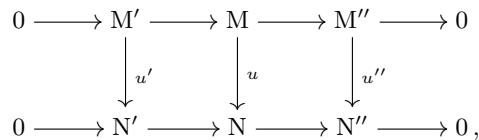
\includegraphics[keepaspectratio]{images/part002_92bb4337.jpg}}

where the first (resp. second) line is an exact sequence of Z{[}G{]}-modules (resp. of Z{[}H{]}-modules) and where \(u', u, u''\) are compatible with \(\varphi\) . Prove that the diagram

\[
\begin{array}{l} \dots \longrightarrow \mathrm{H} ^ {n} (\mathrm{G}, \mathrm{M} ^ {\prime}) \longrightarrow \mathrm{H} ^ {n} (\mathrm{G}, \mathrm{M}) \longrightarrow \mathrm{H} ^ {n} (\mathrm{G}, \mathrm{M} ^ {\prime \prime}) \longrightarrow \mathrm{H} ^ {n + 1} (\mathrm{G}, \mathrm{M} ^ {\prime}) \longrightarrow \dots \\ \Biggl \downarrow_ {\mathrm{H} ^ {n} (\varphi , u ^ {\prime})} \qquad \Biggl \downarrow_ {\mathrm{H} ^ {n} (\varphi , u)} \qquad \Biggl \downarrow_ {\mathrm{H} ^ {n} (\varphi , u ^ {\prime \prime})} \qquad \Biggl \downarrow_ {\mathrm{H} ^ {n + 1} (\varphi , u)} \\ \dots \longrightarrow \mathrm{H} ^ {n} (\mathrm{H}, \mathrm{N} ^ {\prime}) \longrightarrow \mathrm{H} ^ {n} (\mathrm{H}, \mathrm{N}) \longrightarrow \mathrm{H} ^ {n} (\mathrm{H}, \mathrm{N} ^ {\prime \prime}) \longrightarrow \mathrm{H} ^ {n + 1} (\mathrm{H}, \mathrm{N} ^ {\prime}) \longrightarrow \dots \end{array}
\]

(whose horizontal lines are the long exact sequences defined in Exercise 1, c)) is commutative.

\begin{enumerate}
\def\labelenumi{\alph{enumi})}
\setcounter{enumi}{3}
\item
  Examples: If H = G, then the mapping u is compatible with \(Id_{G}\) if and and only if it is Z{[}G{]}-linear, and we have \(\mathrm{H}^{n}(\mathrm{Id}_{\mathrm{G}}, u) = \mathrm{H}^{n}(\mathrm{G}, u)\) . If N is equal to M endowed with the Z{[}G{]}-module structure deduced from \(\varphi\) , then the homomorphisms \(\varphi\) and \(1_{M}\) are compatible; we denote by \(\operatorname{Res}^{q} : \mathrm{H}^{q}(\mathrm{G}, \mathrm{M}) \to \mathrm{H}^{q}(\mathrm{H}, \mathrm{M})\) the homomorphism \(\mathrm{H}^{q}(\varphi, 1_{\mathrm{M}})\) (``restriction homomorphism'').
\item
  Let H be a normal subgroup of G, and let \(M^{H}\) be the subgroup of M consisting of the elements invariant under H, endowed with the action of G/H deduced from that of G by passing to the quotient. The canonical surjection \(p: G \rightarrow G/H\) and the canonical injection \(j: M^{H} \rightarrow M\) are compatible; we denote by \(\operatorname{Inf}^{q}: \operatorname{H}^{q}(\operatorname{G}/\operatorname{H}, \operatorname{M}^{\operatorname{H}}) \to \operatorname{H}^{q}(\operatorname{G}, \operatorname{M})\) the homomorphism \(\operatorname{H}^{q}(p, j)\) (``inflation homomorphism''). Prove that the sequence
\end{enumerate}

\[
0 \to \mathrm{H} ^ {1} (\mathrm{G} / \mathrm{H}, \mathrm{M} ^ {\mathrm{H}}) \xrightarrow {\operatorname{Inf} ^ {1}} \mathrm{H} ^ {1} (\mathrm{G}, \mathrm{M}) \xrightarrow {\operatorname{Res} ^ {1}} \mathrm{H} ^ {1} (\mathrm{H}, \mathrm{M})
\]

is exact. If, moreover, \(\mathrm{H}^1 (\mathrm{H},\mathrm{M})\) is zero, then the sequence

\[
0 \to \mathrm{H} ^ {2} (\mathrm{G} / \mathrm{H}, \mathrm{M} ^ {\mathrm{H}}) \xrightarrow {\operatorname{Inf} ^ {2}} \mathrm{H} ^ {2} (\mathrm{G}, \mathrm{M}) \xrightarrow {\operatorname{Res} ^ {2}} \mathrm{H} ^ {2} (\mathrm{H}, \mathrm{M})
\]

is exact.

¶ 3) Let G be a group and M a Z{[}G{]}-module. Let G act on C \(^{1}\) (G,M) by sending \((g,f)\in\mathrm{G}\times\mathrm{C}^{1}(\mathrm{G},\mathrm{M})\) to the function \(h\mapsto gf(g^{-1}h)\) on G. Recall (I, §6, p.~149, Exercise 8) that a G-mean on M is a Z{[}G{]}-linear mapping \(\mu:C^{1}(\mathrm{G},\mathrm{M})\to\mathrm{M}\) satisfying \(\mu(c_{x})=x\) , where \(c_{x}\) denotes the constant function with value \(x\in\mathrm{M}\) .

\begin{enumerate}
\def\labelenumi{\alph{enumi})}
\item
  Prove that if M admits a G-mean, then \(\mathrm{H}^{n}(\mathrm{G},\mathrm{M})\) is zero for \(n \geqslant 1\) . (For \(q \geqslant 1\) , let \(h^{q}: \mathrm{C}^{q}(\mathrm{G},\mathrm{M}) \to \mathrm{C}^{q-1}(\mathrm{G},\mathrm{M})\) be the following homomorphism: for \(g_{1}, \ldots, g_{q-1}\) in G and \(c \in \mathrm{C}^{q}(\mathrm{G}, \mathrm{M})\) , define \(h^{q}(c)(g_{1}, \ldots, g_{q-1})\) as the image by \(\mu\) of the function \(g \mapsto c(g_{1}, \ldots, g_{q-1}, (g_{1} \cdots g_{q-1})^{-1}g)\) . Prove the equality \(h^{q+1} \circ d^{q} + d^{q-1} \circ h^{q} = 1_{\mathrm{C}^{q}(\mathrm{G}, \mathrm{M})}\) .
\item
  Let A be an abelian group; denote by \(\mathcal{F}(\mathrm{G},\mathrm{A})\) the group of mappings from G to A, endowed with the action of G defined by \({}^{g}f(h)=f(hg)\) for g,h in G and f in \(\mathcal{F}(\mathrm{G},\mathrm{A})\) . For any mapping c from G to \(\mathcal{F}(\mathrm{G},\mathrm{A})\) , denote by \(\mu(c)\) the mapping \(g\mapsto c(g^{-1})(g)\) from G to A. Show that \(\mu\) is a G-mean on \(\mathcal{F}(\mathrm{G},\mathrm{A})\) ; we therefore have \(\mathrm{H}^{q}(\mathrm{G},\mathcal{F}(\mathrm{G},\mathrm{A}))=0\) for \(q\geqslant1\) .
\item
  Let \(j: M \to \mathcal{F}(G, M)\) be the mapping that sends an element m of M to the function \(g \mapsto gm\) , and let \(M'\) be its cokernel. Prove that j is injective and Z{[}G{]}-linear. Deduce that the homomorphism \(\partial^{q}: H^{q}(G, M') \to H^{q+1}(G, M)\) is bijective for \(q \geqslant 1\) .
\item
  Let L be a finite Galois extension of the commutative field K and G be its Galois group. Deduce from b) and the normal basis theorem (V, §10, No.~9, p.~73) that the groups \(\mathrm{H}^{n}(\mathrm{G},\mathrm{L})\) are zero for \(n \geqslant 1\) .
\end{enumerate}

¶ 4) Let G be a group and H a subgroup of G. For any Z{[}H{]}-module N, denote by \(\widetilde{N}\) the group \(\operatorname{Hom}_{\mathbf{Z}[H]}(\mathbf{Z}[G], N)\) endowed with a Z{[}G{]}-module structure deduced from the right Z{[}G{]}-module structure on Z{[}G{]}.

\begin{enumerate}
\def\labelenumi{\alph{enumi})}
\item
  Prove that \(\widetilde{\mathbf{N}}\) can be identified with the \(\mathbf{Z}[\mathrm{G}]\) -submodule of \(\mathcal{F}(\mathrm{G},\mathrm{N})\) (Exercise 3) consisting of the mappings \(f\) such that \(f(hg) = hf(g)\) for every \(h\in \mathrm{H}\) and \(g\in \mathrm{G}\) . If \(\mathrm{A}\) is an abelian group, then the \(\mathbf{Z}[\mathrm{G}]\) -module \(\widetilde{\mathcal{F}(\mathrm{H},\mathrm{A})}\) is canonically isomorphic to \(\mathcal{F}(\mathrm{G},\mathrm{A})\) .
\item
  Let \(0 \rightarrow N' \stackrel{i}{\rightarrow} N \stackrel{p}{\rightarrow} N'' \rightarrow 0\) be an exact sequence of Z{[}H{]}-modules; the sequence
\end{enumerate}

\[
0 \longrightarrow \widetilde {\mathrm{N}} ^ {\prime} \xrightarrow {\operatorname{Hom} (1 , i)} \widetilde {\mathrm{N}} \xrightarrow {\operatorname{Hom} (1 , p)} \widetilde {\mathrm{N}} ^ {\prime \prime} \longrightarrow 0
\]

is exact (observe that the \(\mathbf{Z}[\mathrm{H}]\) -module \(\mathbf{Z}[\mathrm{G}]\) is free).

\begin{enumerate}
\def\labelenumi{\alph{enumi})}
\setcounter{enumi}{2}
\tightlist
\item
  Let \(u_{N} : \widetilde{N} \to N\) be the mapping \(f \mapsto f(1)\) ; it is compatible with the canonical injection \(i : H \to G\) (Exercise 2). Prove that the homomorphism
\end{enumerate}

\[
\mathrm{H} ^ {q} (i, u _ {\mathrm{N}}): \mathrm{H} ^ {q} (\mathrm{G}, \widetilde {\mathrm{N}}) \to \mathrm{H} ^ {q} (\mathrm{H}, \mathrm{N})
\]

is bijective for every \(q \geqslant 0\) (first treat the case q = 0 and then reason by induction on q using the above; Exercise 3, c); and Exercise 2, c)).

\begin{enumerate}
\def\labelenumi{\alph{enumi})}
\setcounter{enumi}{3}
\item
  Suppose that H has finite index n in G. Let M be a Z{[}G{]}-module, which we view as a Z{[}H{]}-module by restriction of scalars. Let \(f \in \widetilde{M}\) ; the element \(g^{-1}f(g)\) depends only on the right class Hg of g. Set \(\pi(f) = \sum_{Hg \in H \setminus G} g^{-1}f(g)\) . Prove that \(\pi\) is a Z{[}G{]}-linear homomorphism from \(\widetilde{M}\) to M. For any integer \(q \geqslant 0\) , denote by \(\operatorname{Cor}^{q}: \mathrm{H}^{q}(\mathrm{H}, \mathrm{M}) \to \mathrm{H}^{q}(\mathrm{G}, \mathrm{M})\) the homomorphism \(\mathrm{H}^{q}(\pi) \circ \mathrm{H}^{q}(i, u_{\mathrm{M}})^{-1}\) (``corestriction homomorphism'').
\item
  Prove that the endomorphism \(Cor^{q} \circ Res^{q}\) of \(H^{q}(G, M)\) is multiplication by n (first treat the case q = 0 and then treat the general case as in the proof of c)).
\item
  Suppose that G is finite; prove that for every Z{[}G{]}-module M and every integer \(q \geqslant 1\) , the group \(\mathrm{H}^{q}(\mathrm{G}, \mathrm{M})\) is annihilated by the order of G.
\end{enumerate}

\begin{enumerate}
\def\labelenumi{\arabic{enumi})}
\setcounter{enumi}{4}
\tightlist
\item
  Let G be a group and M a not necessarily abelian group endowed with a homomorphism \(\varphi: G \to \text{Aut}(M)\) ; for \(g \in G\) and \(m \in M\) , set \(^{g}m = \varphi(g)(m)\) . Denote by \(H^{0}(G, M)\) the subgroup of M consisting of the elements fixed by the action of G; its identity element is called the marked or distinguished element of \(H^{0}(G, M)\) . Let \(Z^{1}(G, M)\) be the set of mappings \(c: G \to M\) satisfying \(c(gh) = c(g)^{g}c(h)\) for g, h in G. For \(c \in Z^{1}(G, M)\) and \(m \in M\) , the mapping \(g \mapsto mc(g)(^g m)^{-1}\) belongs to \(Z^{1}(G, M)\) ; this defines an action of the group M on \(Z^{1}(G, M)\) . The quotient set is denoted by \(H^{1}(G, M)\) ; it is endowed with a marked element, namely the class of the constant mapping with value 1. If M is abelian, then the set \(H^{1}(G, M)\) coincides with that defined in Exercise 1.
\end{enumerate}

\begin{enumerate}
\def\labelenumi{\alph{enumi})}
\item
  Let N be a second group endowed with an action of G and \(u: M \to N\) a group homomorphism compatible with the actions of G. For i = 0, 1, define homomorphisms \(\mathrm{H}^{i}(u): \mathrm{H}^{i}(\mathrm{G}, \mathrm{M}) \to \mathrm{H}^{i}(\mathrm{G}, \mathrm{N})\) that send the marked element of \(\mathrm{H}^{i}(\mathrm{G}, \mathrm{M})\) to that of \(\mathrm{H}^{i}(\mathrm{G}, \mathrm{N})\) .
\item
  Let \(0 \to M' \xrightarrow{\iota} M \xrightarrow{\pi} M'' \to 0\) be an exact sequence of groups with operators in G. Let \(x'' \in \mathrm{H}^0(\mathrm{G}, \mathrm{M}'')\) , and let x be an element of M such that \(\pi(x) = x''\) . Prove that there exists an element \(c' \in \mathrm{Z}^1(\mathrm{G}, \mathrm{M}')\) such that \(\iota \circ c'(g) = g^{-1}c(g)\) for every \(g \in G\) and that the class of \(c'\) in \(\mathrm{H}^1(\mathrm{G}, \mathrm{M}')\) depends only on \(x''\) ; we denote that class by \(\partial(x'')\) . Prove that the sequence
\end{enumerate}

\[
0 \to \mathrm{H} ^ {0} (\mathrm{G}, \mathrm{M} ^ {\prime}) \xrightarrow {\mathrm{H} ^ {0} (\iota)} \mathrm{H} ^ {0} (\mathrm{G}, \mathrm{M}) \xrightarrow {\mathrm{H} ^ {0} (\pi)} \mathrm{H} ^ {0} (\mathrm{G}, \mathrm{M} ^ {\prime \prime}) \xrightarrow {\partial}
\]

\[
\mathrm{H} ^ {1} (\mathrm{G}, \mathrm{M} ^ {\prime}) \xrightarrow {\mathrm{H} ^ {1} (\iota)} \mathrm{H} ^ {1} (\mathrm{G}, \mathrm{M}) \xrightarrow {\mathrm{H} ^ {1} (\pi)} \mathrm{H} ^ {1} (\mathrm{G}, \mathrm{M} ^ {\prime \prime})
\]

is exact (a sequence of mappings \(G \xrightarrow{i} F \xrightarrow{p} E\) , where the set E is endowed with a marked element e, is called exact in F if \(\operatorname{Im}(i) = p^{-1}(e)\) ).

\begin{enumerate}
\def\labelenumi{\alph{enumi})}
\setcounter{enumi}{2}
\item
  Suppose, moreover, that \(M'\) is contained in the center of M. Construct a mapping \(\partial^{1}: H^{1}(G, M'') \to H^{2}(G, M')\) such that the inverse image of the identity element by \(\partial^{1}\) is the image of \(H^{1}(\pi)\) . Also define an action of the group \(H^{1}(G, M')\) on the set \(H^{1}(G, M)\) such that two elements are conjugate for this action if and only if they have the same image by \(H^{1}(\pi)\) .
\item
  Let K be a commutative field, L a finite Galois extension of K with Galois group G, and n an integer. Let G act on the group \(\mathbf{GL}_{n}(\mathrm{L})\) by setting \(\sigma A = (\sigma(a_{ij}))\) for \(\sigma \in G\) and \(A = (a_{ij}) \in \mathbf{GL}_{n}(\mathrm{L})\) . Deduce from V, §10, No.~5, p.~64, Proposition 9 that the set \(\mathrm{H}^{1}(\mathrm{G}, \mathbf{GL}_{n}(\mathrm{L}))\) is reduced to one element (``Hilbert's 90 theorem'').
\end{enumerate}

¶ 6) Let L be a finite Galois extension of the commutative field K, with Galois group G. Let V and V' be K-vector spaces and w (resp. w') a tensor of type \((p,q)\) on V (resp. V'). An L-isomorphism from \((V,w)\) to \((V',w')\) is an L-linear isomorphism \(u:V_{(L)}\to V_{(L)}'\) such that \(u^{\otimes p}\otimes(^{t}u^{-1})^{\otimes q}\) sends the image of w to that of \(w'\) . We denote by \(\operatorname{Aut}_{\mathrm{L}}(\mathrm{V},w)\) the group of L-automorphisms of \((\mathrm{V},w)\) , on which G acts by \(\sigma\varphi=(1_{\mathrm{V}}\otimes\sigma)\circ\varphi\circ(1_{\mathrm{V}}\otimes\sigma)^{-1}\) .

\begin{enumerate}
\def\labelenumi{\alph{enumi})}
\item
  Let u be an L-isomorphism from \((\mathrm{V}, w)\) to \((\mathrm{V}^{\prime}, w^{\prime})\) and \(\sigma\) an element of G; the mapping \(\sigma u = (1_{\mathrm{V}^{\prime}} \otimes \sigma) \circ u \circ (1_{\mathrm{V}} \otimes \sigma)^{-1}\) is an L-isomorphism from \((\mathrm{V}, w)\) to \((\mathrm{V}^{\prime}, w^{\prime})\) , so that \(c(\sigma) = u^{-1} \circ \sigma u\) is an element of \(\operatorname{Aut}_{\mathrm{L}}(\mathrm{V}, w)\) . Prove that the mapping \(c : G \to \operatorname{Aut}_{\mathrm{L}}(\mathrm{V}, w)\) belongs to \(Z^{1}(\mathrm{G}, \operatorname{Aut}_{\mathrm{L}}(\mathrm{V}, w))\) and that its class \(\theta(\mathrm{V}^{\prime}, w^{\prime})\) in \(H^{1}(\mathrm{G}, \operatorname{Aut}_{\mathrm{L}}(\mathrm{V}, w))\) does not depend on the choice of u.
\item
  Prove that the mapping \((\mathrm{V}^{\prime},t^{\prime})\mapsto\theta(\mathrm{V}^{\prime},t^{\prime})\) defines a bijection from the set of K-isomorphism classes of pairs \((\mathrm{V}^{\prime},w^{\prime})\) L-isomorphic to \((\mathrm{V},w)\) to the set \(\mathrm{H}^{1}(\mathrm{G},\mathrm{Aut}_{\mathrm{L}}(\mathrm{V},w))\) . (Given an element c of \(\mathrm{Z}^{1}(\mathrm{G},\mathrm{Aut}_{\mathrm{L}}(\mathrm{V},w))\) , deduce from Exercise 5, d) an L-automorphism f of \(\mathrm{V}_{(\mathrm{L})}\) such that \(c(\sigma)=f^{-1}\circ^{\sigma}f\) . Prove that the image \(w^{\prime}\) of w by the automorphism deduced from f is rational over K, and consider the pair \((\mathrm{V},w^{\prime}).\) )
\end{enumerate}

* c) Examples: The set \(\mathrm{H}^1 (\mathrm{G},\mathbf{Sp}_{2n}(\mathrm{L}))\) is reduced to one element. If Q is a quadratic form on K, then the set \(\mathrm{H}^1 (\mathrm{G},\mathbf{O}(\mathrm{Q}_{(\mathrm{L})}))\) can be identified with the set of equivalence classes of quadratic forms on K equivalent to Q over L.*

\(d\) ) Let A be a K-algebra and M the automorphism group of the L-algebra \(\mathrm{A}_{(\mathrm{L})}\) , endowed with the action of G defined above. The construction in \(b\) ) defines a bijection from the set of isomorphism classes of pairs \((\mathrm{B},u)\) , where B is a K-algebra and \(u\) is an isomorphism from \(\mathrm{B}_{(\mathrm{L})}\) to \(\mathrm{A}_{(\mathrm{L})}\) , to the set \(Z^{1}(\mathrm{G},\mathrm{M})\) . The inverse bijection sends an element \(c\) of \(Z^{1}(\mathrm{G},\mathrm{M})\) to the K-subalgebra of \(\mathrm{A}_{(\mathrm{L})}\) consisting of the elements \(a\) satisfying \(c(\sigma)(\sigma(a)) = a\) for every \(\sigma \in \mathrm{G}\) .

\begin{enumerate}
\def\labelenumi{\arabic{enumi})}
\setcounter{enumi}{6}
\tightlist
\item
  Let L be an extension of K. For any integer \(n \geqslant 1\) , denote by \(\mathcal{A}_{n}(\mathrm{L}/\mathrm{K})\) the set of isomorphism classes of central simple K-algebras of degree \(n^{2}\) split by L.
\end{enumerate}

\begin{enumerate}
\def\labelenumi{\alph{enumi})}
\item
  Prove that the kernel \(\mathrm{Br}(\mathrm{L} / \mathrm{K})\) of the canonical homomorphism \(\mathrm{Br}(\mathrm{K})\to \mathrm{Br}(\mathrm{L})\) is isomorphic to the direct limit of the sets \(\mathcal{A}_n(\mathrm{L} / \mathrm{K})\) ; specify a system of mappings. b) Assume from now on that L is a finite Galois extension of K, with Galois group G. Deduce a bijection \(\theta_{n}:\mathcal{A}_{n}(\mathrm{L} / \mathrm{K})\to \mathrm{H}^{1}(\mathrm{G},\mathbf{PGL}_{n}(\mathrm{L}))\) from Exercise 6.
\item
  Denote by \(\partial_n: \mathrm{H}^1(\mathrm{G}, \mathbf{PGL}_n(\mathrm{L})) \to \mathrm{H}^2(\mathrm{G}, \mathrm{L}^*)\) the mapping deduced from the exact sequence \(1 \to \mathrm{L}^* \to \mathbf{GL}_n(\mathrm{L}) \to \mathbf{PGL}_n(\mathrm{L}) \to 1\) (Exercise 5, c)) and by \(\delta_n: \mathcal{A}_n(\mathrm{L/K}) \to \mathrm{H}^2(\mathrm{G}, \mathrm{L}^*)\) the mapping \(\partial_n \circ \theta_n\) . If \(\mathrm{A} \in \mathcal{A}_n(\mathrm{L/K})\) , then we have \(\delta_n(\mathrm{A}) = 0\) if and only if \(\mathrm{A}\) is a matrix algebra over \(\mathrm{K}\) ; if \(\mathrm{A} \in \mathcal{A}_p(\mathrm{L/K})\) and \(\mathrm{B} \in \mathcal{A}_q(\mathrm{L/K})\) , then we have \(\delta_{pq}(\mathrm{A} \otimes_{\mathrm{K}} \mathrm{B}) = \delta_p(\mathrm{A}) + \delta_q(\mathrm{B})\) . Deduce an injective group homomorphism \(\delta_{\mathrm{L/K}}: \mathrm{Br}(\mathrm{L/K}) \to \mathrm{H}^2(\mathrm{G}, \mathrm{L}^*)\) by passing to the direct limit. d) Prove that \(\partial_n\) is surjective for \(n = \operatorname{Card}(\mathrm{G})\) . (Let \(c: \mathrm{G} \times \mathrm{G} \to \mathrm{L}^*\) be an element of \(\mathrm{Z}^2(\mathrm{G}, \mathrm{L}^*)\) . For every \(\sigma \in \mathrm{G}\) , consider the endomorphism \(u(\sigma)\) of \(\mathrm{L}^{\mathrm{G}}\) that sends \(e_\tau\) to \(c(\sigma, \tau)e_{\sigma\tau}\) for every \(\tau \in \mathrm{G}\) , and determine \(u(\sigma)^{\sigma}u(\tau)u(\sigma\tau)^{-1}\) .)
\item
  Compare \(\delta_{\mathrm{L / K}}\) and \(\Phi_{\mathrm{L / K}}\) .
\item
  Prove that the group \(\mathrm{Br}(\mathrm{K})\) can be identified with the limit of the direct system of groups \(\left(\mathrm{H}^{2}(\mathrm{Gal}(\mathrm{L}/\mathrm{K}),\mathrm{L}^{*})\right)\) with respect to the set (ordered by inclusion) of finite Galois extensions of K contained in a fixed algebraic closure of K, where the homomorphisms between these groups are the (injective) inflation homomorphisms. g) Let F be an extension of K contained in L and \(\Gamma\) the subgroup of G that leaves F invariant. Prove that the following diagram commutes:
\end{enumerate}

\[
\begin{array}{c} \operatorname{Br} (\mathrm{L} / \mathrm{K}) \xrightarrow {r _ {\mathrm{F} / \mathrm{K}}} \operatorname{Br} (\mathrm{F} / \mathrm{L}) \\ \Biggl \downarrow_ {\delta_ {\mathrm{L} / \mathrm{K}}} \qquad \qquad \qquad \qquad \Biggl \downarrow_ {\delta_ {\mathrm{F} / \mathrm{L}}} \\ \operatorname{H} ^ {2} (\operatorname{G}, \operatorname{L} ^ {*}) \xrightarrow {\operatorname{Res} ^ {2}} \operatorname{H} ^ {2} (\Gamma , \operatorname{L} ^ {*}). \end{array}
\]

Deduce a canonical isomorphism from \(\mathrm{Br}(\mathrm{F}/\mathrm{K})\) to the kernel of the homomorphism \(\mathrm{Res}^{2}:\mathrm{H}^{2}(\mathrm{G},\mathrm{L}^{*})\to\mathrm{H}^{2}(\Gamma,\mathrm{L}^{*})\) .

\begin{enumerate}
\def\labelenumi{\arabic{enumi})}
\setcounter{enumi}{7}
\item
  Let L be an extension of K. Suppose that K has characteristic p \textgreater{} 0 and \(L = K^{1/p}\) . Prove that the group \(\mathrm{Br}(\mathrm{L}/\mathrm{K})\) is equal to the kernel of multiplication by p in \(\mathrm{Br}(\mathrm{K})\) (observe that if N is a finite Galois extension of K, then \(N^{1/p}\) is a Galois extension of L with the same Galois group).
\item
  Let G be a finite group and M a Z{[}G{]}-module. Denote by \(N_{G}\) the homomorphism \(m \mapsto \sum_{g} gm\) from M to M; its image is contained in the submodule \(M^{G}\) of M consisting of the invariant elements. Let \(\mathrm{T}_{\mathrm{G}}(\mathrm{M})\) be the quotient group \(\mathrm{M}^{\mathrm{G}}/\mathrm{N}_{\mathrm{G}}(\mathrm{M})\) . a) Let \(c \in \mathrm{Z}^{2}(\mathrm{G}, \mathrm{M})\) . Prove that the element \(\sum_{h} c(h, g)\) belongs to \(M^{G}\) ; we denote its class in \(\mathrm{T}_{\mathrm{G}}(\mathrm{M})\) by \(\theta_{c}(g)\) . Prove that \(\theta_{c}\) is a homomorphism from G to \(\mathrm{T}_{\mathrm{G}}(\mathrm{M})\) that is zero when \(c \in \mathrm{B}^{2}(\mathrm{G}, \mathrm{M})\) . Deduce a homomorphism \(\theta_{\mathrm{M}} : \mathrm{H}^{2}(\mathrm{G}, \mathrm{M}) \to \mathrm{Hom}(\mathrm{G}, \mathrm{T}_{\mathrm{G}}(\mathrm{M}))\) from it.
\end{enumerate}

\begin{enumerate}
\def\labelenumi{\alph{enumi})}
\setcounter{enumi}{1}
\tightlist
\item
  Let \(u: M \to N\) be a homomorphism of Z{[}G{]}-modules and \(\widetilde{u}: T_{G}(M) \to T_{G}(N)\) the homomorphism induced by u. Prove that we have \(\theta_{\mathrm{N}} \circ \mathrm{H}^{2}(u) = \mathrm{Hom}(1_{\mathrm{G}}, \widetilde{u}) \circ \theta_{\mathrm{M}}\) . c) Assume from now on that G is cyclic; let \(\sigma\) be a generator of G, and denote its order by n.~Let \(\chi \in \mathrm{Hom}(G, \mathbf{Z}/n\mathbf{Z})\) be the homomorphism that sends \(\sigma\) to the class of 1, and let \(\lambda \in H^{2}(G, \mathbf{Z})\) be its image by the connecting homomorphism associated with the exact sequence \(0 \to Z \to Z \to Z/nZ \to 0\) . Prove that \(\lambda\) is the class of the element \(\varepsilon \in Z^{2}(G, \mathbf{Z})\) such that for \(0 \leqslant p < n\) and \(0 \leqslant q < n\) , the image \(\varepsilon(\sigma^{p}, \sigma^{q})\) is equal to 0 if \(p + q < n\) and to 1 if \(p + q \geqslant n\) . For \(m \in M^{G}\) , denote by \(h_{m}\) the Z{[}G{]}-linear mapping from Z to M such that \(h_{m}(1) = m\) . Prove that the image of \(H^{2}(h_{m})(\lambda)\) by \(\theta_{M}\) is equal to the class of m, so that \(\theta_{M}\) is surjective.
\end{enumerate}

\(d\) ) Prove that \(\theta_{\mathrm{M}}\) is an isomorphism. (Let \(c\in \mathbf{Z}^2 (\mathrm{G},\mathrm{M})\) . Prove that we may assume \(c(g,1) = c(1,g) = 1\) for every \(g\in \mathrm{G}\) , and determine the images by \(d^1\) of the elements \(b\) and \(a_{m}\) \((m\in \mathrm{M})\) of \(\mathrm{C}^1 (\mathrm{G},\mathrm{M})\) defined by \(b(\sigma^{p}) = \sum_{i = 0}^{p - 1}c(\sigma^{i},\sigma)\) and \(a_{m}(\sigma^{p}) = \sum_{i = 0}^{p - 1}\sigma^{i}m.)\)

\begin{enumerate}
\def\labelenumi{\arabic{enumi})}
\setcounter{enumi}{9}
\tightlist
\item
  \begin{enumerate}
  \def\labelenumii{\alph{enumii})}
  \tightlist
  \item
    Let L be a cyclic extension of K. Deduce from Exercises 9 and 7 that the groups Br(L/K) and \(K^{*}/N_{L/K}(L^{*})\) are isomorphic.
  \end{enumerate}
\end{enumerate}

\begin{enumerate}
\def\labelenumi{\alph{enumi})}
\setcounter{enumi}{1}
\item
  Suppose that every extension L of K of finite degree is cyclic and that the norm mapping \(N_{L/K}: L^{*} \to K^{*}\) is surjective. Prove that every field extension of K of finite degree with center K is equal to K.
\item
  Apply the previous question to finite fields.
\end{enumerate}

\begin{enumerate}
\def\labelenumi{\arabic{enumi})}
\setcounter{enumi}{10}
\tightlist
\item
  Let L be a cyclic extension of K with Galois group G, and let \(\sigma\) be a generator of G. Exercise 10 gives a canonical isomorphism \(\mathrm{Br}(\mathrm{L}/\mathrm{K}) \to \mathrm{K}^{*}/\mathrm{N}_{\mathrm{L}/\mathrm{K}}(\mathrm{L}^{*})\) , whose inverse we will now construct explicitly.
\end{enumerate}

Let \(\theta \in \mathrm{K}^*\) , and let \(c_{\theta} \in \mathrm{Z}^{2}(\mathrm{G}, \mathrm{L}^{*})\) be the element defined by \(c_{\theta}(\sigma^{p}, \sigma^{q}) = \theta^{\varepsilon(p,q)}\) (Exercise 9, \(c\) )). Prove that the cross product A{[} \(\mathcal{E}\) , L{]} of L and the extension \(\mathcal{E}\) associated with \(c_{\theta}\) is isomorphic to the quotient of the K-algebra L{[}X{]} \(_{\sigma}\) (VIII, p.~11) by the (two-sided) ideal generated by the central element X \(^{n}\) - \(\theta\) . The class of A \(_{\theta}\) in Br(L/K) corresponds to the class of \(\theta\) ( \(\text{mod } \mathrm{N}_{\mathrm{L/K}}(\mathrm{L}^{*})\) ) by the isomorphism defined above.

\begin{enumerate}
\def\labelenumi{\arabic{enumi})}
\setcounter{enumi}{11}
\tightlist
\item
  Let A be a commutative ring. Endow the set of isomorphism classes of Azumaya A-algebras (VIII, p.~270, Exercise 8) with the structure of a monoid by setting \(\operatorname{cl}(S)\operatorname{cl}(T)=\operatorname{cl}(S\otimes_{A}T)\) .
\end{enumerate}

\begin{enumerate}
\def\labelenumi{\alph{enumi})}
\item
  Prove that the quotient monoid for Morita equivalence is an abelian group; we denote it by Br(A) and call it the Brauer group of A (when A is a field, this definition coincides with that given in VIII, p.~279). Denote by {[}S{]} the class of an Azumaya A-algebra S in Br(A). The identity element of Br(A) is the class of A, and the inverse of an element {[}S{]} is {[}S°{]}.
\item
  Let S be an Azumaya A-algebra. We have \([S] = [A]\) if and only if there exists a finitely generated, projective, faithful A-module P such that S is isomorphic to \(\operatorname{End}_{\mathrm{A}}(\mathrm{P})\) .
\item
  Let B be a commutative A-algebra. Define a group homomorphism \(r_{B/A} : \mathrm{Br}(A) \to \mathrm{Br}(B)\) such that \(r_{\mathrm{B/A}}([\mathrm{S}]) = [\mathrm{S}_{(\mathrm{B})}]\) for every Azumaya A-algebra S. We denote the kernel of this homomorphism by \(\mathrm{Br(B/A)}\) .
\end{enumerate}

¶ 13) Let A be a commutative ring, B a commutative A-algebra, and G a finite group of automorphisms of the A-algebra B. Suppose that B is a finitely generated, projective, faithful A-module and that the A-linear homomorphism \(\psi : \mathrm{B} \otimes_{\mathrm{A}} \mathrm{B} \to \mathrm{B}^{\mathrm{G}}\) defined by \(\psi(b \otimes b') = (\sigma(b)b')_{\sigma \in \mathrm{G}}\) is bijective.

\begin{enumerate}
\def\labelenumi{\alph{enumi})}
\item
  Let N be a B-module, endowed with a homomorphism \(\sigma \mapsto u_{\sigma}\) from G to \(\mathrm{Aut}_{\mathrm{A}}(\mathrm{N})\) satisfying \(u_{\sigma}(bx) = \sigma(b)u_{\sigma}(x)\) for \(\sigma \in \mathrm{G}\) , \(b \in \mathrm{B}\) , \(x \in \mathrm{N}\) . Let M be the A-submodule of N consisting of the elements \(x\) such that \(u_{\sigma}(x) = x\) for every \(\sigma \in \mathrm{G}\) . Prove that the canonical B-homomorphism \(\mathrm{B} \otimes_{\mathrm{A}} \mathrm{M} \to \mathrm{N}\) is bijective (use Exercise 7, \(d\) ) of VIII, p.~270 to reduce to the case when B is the product algebra \(\mathrm{A}^{\mathrm{G}}\) on which G acts by permuting the factors).
\item
  Let S be an A-algebra and M the automorphism group of the B-algebra \(\mathrm{S}_{(\mathrm{B})}\) , on which G acts by \(\sigma\varphi = (\mathrm{Id}_{\mathrm{S}} \otimes \sigma) \circ \varphi \circ (\mathrm{Id}_{\mathrm{S}} \otimes \sigma)^{-1}\) . Extend the construction of Exercise 6 to define a bijection from the set of isomorphism classes of pairs \((T,u)\) , where T is an A-algebra and u an isomorphism from \(T_{(B)}\) to \(S_{(B)}\) , to the set \(Z^{1}(G,M)\) , as well as a bijection from the set of isomorphism classes of A-algebras T such that the B-algebras \(T_{(B)}\) and \(S_{(B)}\) are isomorphic to \(H^{1}(G,M)\) .
\item
  Assume from now on that every projective B-module is free. Adapt the reasoning of Exercise 8 to construct an isomorphism \(\theta : \mathrm{Br}(\mathrm{B} / \mathrm{A}) \to \mathrm{H}^2(\mathrm{G}, \mathrm{B}^*)\) .
\end{enumerate}

¶ 14) Let A be a Noetherian commutative local ring, m its maximal ideal, \(\kappa\) the field A/m, and S an Azumaya algebra over A.

\begin{enumerate}
\def\labelenumi{\alph{enumi})}
\item
  Let \(e\) be an idempotent in S whose image in S/mS is an indecomposable idempotent. Deduce from Nakayama's lemma (cf.~VIII, p.~168, Exercise 16) that the canonical homomorphism \(S \to \mathrm{End}_{\mathrm{A}}(Se)\) is bijective.
\item
  Suppose that m is nilpotent \(^{*}\) (or, more generally, that A is complete for the m-adic topology) \(^{*}\) . Prove that the homomorphism \(r_{\kappa/A}: \mathrm{Br}(A) \to \mathrm{Br}(\kappa)\) is injective.
\end{enumerate}

* \(c\) ) Assume from now on that A is complete. Let L be a separable extension of \(\kappa\) of finite degree that is a splitting field for the \(\kappa\) -algebra S/mS. Let \(x\) be a primitive element of L, \(f\) its minimal polynomial, F a monic polynomial in A{[}X{]} whose image in \(\kappa\) {[}X{]} is \(f\) , and B = A{[}X{]}/(F). Prove that B is a local A-algebra, free and finitely generated as an A-module, with maximal ideal mB and residue field isomorphic to L; the B-algebra S \(_{(B)}\) is isomorphic to a matrix algebra.

\(d\) ) Suppose, moreover, that L is a Galois extension of \(\kappa\) , with Galois group G. Prove that the action of G on L lifts to an action on the A-algebra B (let \(G'\) be the automorphism group of this algebra; deduce from Hensel's lemma (Comm. Alg., III, §4, No.~3, p.~215, Theorem 1) that the natural homomorphism \(G' \to G\) is bijective). Deduce from Nakayama's lemma that the homomorphism \(\psi : B \otimes_A B \to B^G\) defined in Exercise 13 is bijective.

\begin{enumerate}
\def\labelenumi{\alph{enumi})}
\setcounter{enumi}{4}
\item
  Prove that the homomorphism \(\mathrm{H}^{q}(\pi):\mathrm{H}^{q}(\mathrm{G},\mathrm{B}^{*})\to\mathrm{H}^{q}(\mathrm{G},\mathrm{L}^{*})\) is bijective for every \(q\geqslant1\) . (For \(i\geqslant1\) , let \(U^{i}\) be the subgroup of elements b of \(B^{*}\) such that \(b\equiv1\) (mod \(m^{i}B\) ). Observe that the Z{[}G{]}-module \(U^{i}/U^{i+1}\) is isomorphic to \(m^{i}B/m^{i+1}B\) , hence to a power of L, and deduce from Exercise 5, d) that \(\mathrm{H}^{q}(\mathrm{G},\mathrm{U}^{i}/\mathrm{U}^{i+1})\) is zero for \(q\geqslant1\) . Let \(c\in\mathrm{Z}^{q}(\mathrm{G},\mathrm{U}^{1})\) . Construct, by induction, a sequence \((b_{n})\) with \(b_{n}\in\mathrm{Z}^{q-1}(\mathrm{G},\mathrm{U}^{n})\) such that \(c-d^{q-1}(\sum_{i=1}^{n}b_{i})\) belongs to \(\mathrm{Z}^{q}(\mathrm{G},\mathrm{U}^{n+1})\) . Conclude that \(\mathrm{H}^{q}(\mathrm{G},\mathrm{U}^{1})\) is zero for \(q\geqslant1\) .
\item
  Conclude that the canonical homomorphisms \(\mathrm{Br}(B/A)\to \mathrm{Br}(L/\kappa)\) and \(\mathrm{Br}(A)\to \mathrm{Br}(\kappa)\) are bijective.*
\end{enumerate}

\begin{enumerate}
\def\labelenumi{\arabic{enumi})}
\setcounter{enumi}{14}
\tightlist
\item
  *a) Let A be a regular integral domain (AC, X, §4, n° 2, p.~55) and K its field of fractions. The homomorphism \(r_{\mathrm{K / A}}: \mathrm{Br(A)} \to \mathrm{Br(K)}\) is injective (VIII, p.~271, Exercise 11).*
\end{enumerate}

\begin{enumerate}
\def\labelenumi{\alph{enumi})}
\setcounter{enumi}{1}
\tightlist
\item
  Prove that the ring \(A = \mathbf{Q}[X, Y]/(X^{2} + Y^{2})\) is an integral domain; let K be its field of fractions. Let H be the quaternion algebra of type \((-1, 0, -1)\) over Q, which is a field (cf.~III, §2, No.~5, p.~445). Prove that the class of the Azumaya
\end{enumerate}

A-algebra \(\mathrm{H}_{(\mathrm{A})}\) in \(\mathrm{Br}(\mathrm{A})\) is not zero but that \(\mathrm{H}_{(\mathrm{K})}\) is isomorphic to \(\mathbf{M}_{2}(\mathrm{K})\) , so that the homomorphism \(r_{K/A}\) is not injective (observe that K contains an element of square -1).

\begin{enumerate}
\def\labelenumi{\arabic{enumi})}
\setcounter{enumi}{15}
\tightlist
\item
  \begin{enumerate}
  \def\labelenumii{\alph{enumii})}
  \tightlist
  \item
    Prove that the homomorphism \(r_{\mathrm{K[X]}/\mathrm{K}} : \mathrm{Br}(\mathrm{K}) \to \mathrm{Br}(\mathrm{K}[\mathrm{X}])\) induces an isomorphism from \(\mathrm{Br}(\mathrm{K})\) to a direct factor of \(\mathrm{Br}(\mathrm{K}[\mathrm{X}])\) .
  \end{enumerate}
\end{enumerate}

\(^{*}b\) ) Suppose that the field K is perfect. Prove that \(r_{K[X]/K}\) is an isomorphism (deduce from Tsen's theorem (VIII, p.~360, Exercise 7) that \(\mathrm{Br}(\mathrm{K}[\mathrm{X}])\) is the union of the groups \(\mathrm{Br}(\mathrm{L}[\mathrm{X}]/\mathrm{K}[\mathrm{X}])\) , where L runs through the Galois extensions of K of finite degree, and then apply Exercise 13).

\begin{enumerate}
\def\labelenumi{\alph{enumi})}
\setcounter{enumi}{2}
\tightlist
\item
  Let A be a regular Q-algebra that is an integral domain. Prove that the homomorphism \(r_{\mathrm{A[X]}/\mathrm{A}} : \mathrm{Br}(\mathrm{A}) \to \mathrm{Br}(\mathrm{A}[\mathrm{X}])\) is bijective (use b) and Exercise 15 to prove that the homomorphism \(\mathrm{Br}(\mathrm{A}[\mathrm{X}]) \to \mathrm{Br}(\mathrm{A})\) deduced from the surjection \(\mathrm{P} \mapsto \mathrm{P}(0)\) is injective).*
\end{enumerate}

\(d\) ) Suppose that K has characteristic \(p > 0\) and is not perfect; let \(\theta \in \mathrm{K} - \mathrm{K}^p\) . View \(\mathrm{B} = \mathrm{K}[\mathrm{U}]\) as a K{[}X{]}-algebra via the homomorphism \(\rho : \mathrm{K}[\mathrm{X}] \to \mathrm{B}\) determined by \(\rho (\mathrm{X}) = \mathrm{U}^p - \mathrm{U}\) . Let \(\sigma\) be the automorphism of this K{[}X{]}-algebra such that \(\sigma (\mathrm{U}) = \mathrm{U} + 1\) , and let S be the quotient K{[}X{]}-algebra of B{[}V{]}\(_{\sigma}\) (VIII, p.~11) by the two-sided ideal B(\(V^{p} - \theta\)). Let L be a K{[}X{]}-algebra that is a commutative field. Prove that if the equation \(y^p - y = X\) has a solution in L, then S\(_{(L)}\) is a matrix algebra over L (let L' = L{[}t{]}/(\(t^{p} - \theta\)); consider the homomorphism S → End\(_{\mathrm{L}}\) (L') that sends V to the multiplication \(m_t\) by t and U to \(m_y\) - D, where D is the L-derivation of L' such that D(t) = t). In the opposite case, S\(_{(L)}\) is a central simple L-algebra; it is a matrix algebra if and only if \(\theta\) is the norm of an element of the extension L{[}Y{]}/(\(Y^{p} - Y - X\)) of L (apply Exercise 11).

Deduce that S is an Azumaya K{[}X{]}-algebra and that its class in \(\mathrm{Br}(\mathrm{K}[\mathrm{X}])\) does not come from \(\mathrm{Br}(\mathrm{K})\) (take \(L = K(X)\) ).

*17) Suppose that the field K is complete for a discrete valuation \(v\) , assumed normed (cf.~Exercise 12 of VIII, p.~272); denote the ring of \(v\) by A and its residue field by \(\kappa\) . The homomorphism \(r_{\kappa / \mathrm{A}}: \mathrm{Br}(\mathrm{A}) \to \mathrm{Br}(\kappa)\) is bijective (Exercise 14); denote by \(\iota: \mathrm{Br}(\kappa) \to \mathrm{Br}(\mathrm{K})\) the homomorphism \(r_{\mathrm{A / K}} \circ r_{\kappa / \mathrm{A}}^{-1}\) .

\begin{enumerate}
\def\labelenumi{\alph{enumi})}
\tightlist
\item
  Let L be an unramified Galois extension of K of finite degree, with Galois group G. Let B be the valuation ring of \(v_{L}\) extending v and \(\kappa_{L}\) be its residue field. The homomorphism \(\iota\) induces a homomorphism \(\iota_{\mathrm{L}} : \mathrm{Br}(\kappa_{\mathrm{L}}/\kappa) \to \mathrm{Br}(\mathrm{L}/\mathrm{K})\) . Construct a split exact sequence
\end{enumerate}

\[
0 \to \mathrm{Br} (\kappa_ {\mathrm{L}} / \kappa) \xrightarrow {\iota_ {\mathrm{L}}} \mathrm{Br} (\mathrm{L} / \mathrm{K}) \to \mathrm{H} ^ {2} (\mathrm{G}, \mathbf {Z}) \to 0,
\]

where Z is endowed with the trivial action of G (observe that the exact sequence of Z{[}G{]}-modules \(0 \rightarrow B^{*} \rightarrow L^{*} \xrightarrow{v_{L}} Z\) splits, and use Exercise 14).

\begin{enumerate}
\def\labelenumi{\alph{enumi})}
\setcounter{enumi}{1}
\item
  Let G be a group. Using the exact sequence \(0 \rightarrow Z \rightarrow Q \rightarrow Q/Z \rightarrow 0\) , prove that the linking homomorphism of Exercise 1 induces an isomorphism from \(\operatorname{Hom}(G, \mathbf{Q}/\mathbf{Z})\) to \(\mathrm{H}^{2}(\mathrm{G}, \mathbf{Z})\) .
\item
  Conclude that we have a split exact sequence
\end{enumerate}

\[
0 \to \mathrm{Br} (\kappa) \stackrel {\iota} {\to} \mathrm{Br} (\mathrm{K}) \to \Xi (\mathfrak {g}, \mathbf {Q} / \mathbf {Z}) \to 0,
\]

where g is the Galois group of a separable closure of \(\kappa\) over \(\kappa\) and \(\Xi(\mathfrak{g})\) is the group of continuous homomorphisms from g to Q/Z, endowed with the discrete topology (pass to the direct limit using Exercise 12 of VIII, p.~272 and the fact that every finite Galois extension of \(\kappa\) is the residue field extension of an unramified finite Galois extension of K, unique up to isomorphism).

\(d\) ) Deduce that \(\operatorname {Br}(\mathrm{K}) = \{0\}\) if \(\kappa\) is algebraically closed.

\begin{enumerate}
\def\labelenumi{\alph{enumi})}
\setcounter{enumi}{4}
\tightlist
\item
  Suppose that the field \(\kappa\) is finite, in other words, that K is a finite extension of a p-adic field or a field of formal power series over a finite field. Construct an isomorphism from \(\mathrm{Br}(\mathrm{K})\) to \(Q/Z\).*
\end{enumerate}

\section{Reduced Norms and Traces}

In this section, K is a commutative field and A a central simple K-algebra of finite degree. We denote the reduced degree of A by n.

\subsection{Complements on Characteristic Polynomials}

Let L be a commutative ring and M a free L-module of finite rank m. If u is an endomorphism of M and r a natural number, then we denote by \(c_{r}(u)\) the trace of the endomorphism \(\wedge^{r}(u)\) of the free L-module \(\wedge^{r}(\mathrm{M})\) . In particular, we have

\[
c _ {0} (u) = 1, \quad c _ {1} (u) = \mathrm{Tr} (u), \quad c _ {m} (u) = \det (u),\tag{1}
\]

and \(c_{r}(u) = 0\) for r \textgreater{} m. By Proposition 7 of III, §8, No.~4, p.~527, the mapping \(u \mapsto \det(u)\) from End(M) to L is a homogeneous polynomial mapping of degree m (IV, §5, No.~9, p.~55). More generally, for every integer r such that \(0 \leqslant r \leqslant m\) , the mapping \(c_{r}\) from End(M) to L is a homogeneous polynomial mapping of degree r; this follows from Proposition 10 of III, §8, No.~5, p.~529.

Let \(u\) be an endomorphism of \(M\) and \(\overline{u}\) the endomorphism of the \(L[X]\) -module \(M[X] = M \otimes_{L} L[X]\) deduced from \(u\) by extension of scalars (II, §5, No.~1, p.~277). Recall (III, §8, No.~11, p.~541, Definition 3 and (50)) that the characteristic polynomial of \(u\) is the determinant \(\chi_u(X)\) of the \(L[X]\) -endomorphism \(X - \overline{u}\) of \(M[X]\) and that we have the relation

\[
\chi_ {u} (\mathrm{X}) = \sum_ {r = 0} ^ {m} (- 1) ^ {r} c _ {r} (u) \mathrm{X} ^ {m - r}.\tag{2}
\]

PROPOSITION 1. --- Let L be a commutative ring, M a free L-module of finite rank \(m \geqslant 1\) , and u an endomorphism of M. There exists a unique endomorphism \(\widetilde{u}\) of M satisfying the relation

\[
\widetilde {u} (x) \wedge w = x \wedge \wedge^ {m - 1} (u) (w)\tag{3}
\]

for \(x\in \mathrm{M}\) and \(w\in \bigwedge^{m - 1}(\mathrm{M})\) . Moreover, we have the relations

\[
u \circ \widetilde {u} = \widetilde {u} \circ u = \det (u) _ {\mathrm{M}},\tag{4}
\]

\[
\det (\widetilde {u}) = \det (u) ^ {m - 1},\tag{5}
\]

\[
\widetilde {u} = \sum_ {r = 0} ^ {m - 1} (- 1) ^ {r} c _ {m - 1 - r} (u) u ^ {r}.\tag{6}
\]

Lemma 1. --- Let p be an integer such that \(0 \leqslant p \leqslant m\) . For any w in \(\wedge^{p}(\mathrm{M})\) , let \(h_{p}(w)\) be the linear mapping \(w' \mapsto w \wedge w'\) from \(\wedge^{m-p}(\mathrm{M})\) to \(\wedge^{m}(\mathrm{M})\) . The linear mapping \(h_{p}: w \mapsto h_{p}(w)\) from \(\wedge^{p}(\mathrm{M})\) to \(\operatorname{Hom}_{\mathrm{L}}(\wedge^{m-p}(\mathrm{M}), \wedge^{m}(\mathrm{M}))\) is an isomorphism.

Let \((e_{i})_{i\in\mathrm{I}}\) be a basis of M; we endow the set I with a total order. For any subset J of I, set \(e_{\mathrm{J}}=e_{i_{1}}\wedge\cdots\wedge e_{i_{r}}\) , where \((i_{1},\ldots,i_{r})\) is the sequence of elements of J in increasing order. The L-module \(\wedge^{m-p}(\mathrm{M})\) admits as a basis the elements \(e_{\mathrm{S}}\) , where S runs through the set of subsets of I with m-p elements; \(\wedge^{m}(\mathrm{M})\) has \(\{e_{\mathrm{I}}\}\) as a basis. Consequently, there exists a basis of \(\mathrm{Hom}_{\mathrm{L}}(\wedge^{m-p}(\mathrm{M}),\wedge^{m}(\mathrm{M}))\) consisting of linear mappings \(e_{\mathrm{J}}^{*}\) characterized by the formula

\[
e _ {\mathrm{J}} ^ {*} (e _ {\mathrm{S}}) = \left\{ \begin{array}{l l} e _ {\mathrm{I}} & \text {if } I = J\cup S, \\ 0 & \text {otherwise}, \end{array} \right.\tag{7}
\]

where J runs through the set of subsets of I with p elements. It follows from formula (20) of III, §7, No.~8, p.~519 that for every subset J of I with p elements, we have \(h_{p}(e_{\mathrm{J}}) \in \{e_{\mathrm{J}}^{*}, -e_{\mathrm{J}}^{*}\}\) ; since the elements \(e_{J}\) form a basis of \(\Lambda^{p}(\mathrm{M})\) , the linear mapping \(h_{p}\) is bijective.

Let us now prove Proposition 1. Let \(u\) and \(\widetilde{u}\) be endomorphisms of M. Relation (3) is equivalent to

\[
h _ {1} \circ \widetilde {u} = \operatorname{Hom} (\wedge^ {m - 1} (u) \cdot 1 _ {\bigwedge^ {m} (\mathrm{M})}) \circ h _ {1};\tag{8}
\]

the mapping \(h_{1}\) is an isomorphism from M to \(\operatorname{Hom}_{\mathrm{L}}(\wedge^{m-1}(\mathrm{M}),\wedge^{m}(\mathrm{M}))\) by Lemma 1. Consequently, for every endomorphism u of M, there exists a unique endomorphism \(\widetilde{u}\) of M satisfying relation (3).

Let \(x_{1},\ldots,x_{m}\) be elements of M. Let us replace x with \(u(x_{1})\) and w with \(x_{2}\wedge\cdots\wedge x_{m}\) in (3); we obtain

\[
\widetilde {u} (u (x _ {1})) \wedge x _ {2} \wedge \dots \wedge x _ {m} = u (x _ {1}) \wedge \dots \wedge u (x _ {m}) = \det (u) x _ {1} \wedge \dots \wedge x _ {m}.
\]

Consequently, \(h_1(\widetilde{u} \circ u(x_1)) = h_1(\det(u)x_1)\) , which gives the relation \(\widetilde{u} \circ u = \det(u)_\mathrm{M}\) by Lemma 1.

We denote by U the endomorphism \(X - \overline{u}\) of the L{[}X{]}-module M{[}X{]} (VIII, p.~335). By the above applied to U, there exists an endomorphism \(\widetilde{U}\) of the L{[}X{]}-module M{[}X{]} that satisfies the relations

\[
\widetilde {\mathrm{U}} (x _ {1}) \wedge x _ {2} \wedge \dots \wedge x _ {m} = x _ {1} \wedge (\mathrm{X} x _ {2} - u (x _ {2})) \wedge \dots \wedge (\mathrm{X} x _ {m} - u (x _ {m}))\tag{9}
\]

for \(x_{1},\ldots ,x_{m}\) in M and

\[
\widetilde {\mathrm{U}} \circ \mathrm{U} = \det (\mathrm{X} - \overline {{u}}) _ {\mathrm{M} [ \mathrm{X} ]}.\tag{10}
\]

Let us view \(\widetilde{\mathbf{U}}\) as an element of \(\operatorname{End}(\mathbf{M})[\mathbf{X}]\) (VIII, p.~9); by formula (9) and Lemma 1, it has degree \(\leqslant m - 1\) , so we can write it as

\[
\widetilde {\mathrm{U}} = \sum_ {r = 0} ^ {m - 1} (- 1) ^ {r} u _ {r} X ^ {m - 1 - r},\tag{11}
\]

where the \(u_{r}\) are endomorphisms of M. By formula (2), relation (10) gives the equality

\[
\left(\sum_ {r = 0} ^ {m - 1} (- 1) ^ {r} u _ {r} \mathrm{X} ^ {m - 1 - r}\right) (\mathrm{X} - u) = \sum_ {r = 0} ^ {m} (- 1) ^ {r} c _ {r} (u) \mathrm{X} ^ {m - r}\tag{12}
\]

in the ring \(\operatorname{End}(M)[X]\) . By identifying the coefficients of the monomials in X on each side, we obtain the relations

\[
u _ {r} + u _ {r - 1} \circ u = c _ {r} (u) _ {\mathrm{M}} \qquad \mathrm{for} 1 \leqslant r \leqslant m - 1\tag{13}
\]

and

\[
u _ {0} = c _ {0} (u) _ {\mathrm{M}}, \quad u _ {m - 1} \circ u = c _ {m} (u) _ {\mathrm{M}}.\tag{14}
\]

From this, we deduce

\[
u _ {m - 1} = \sum_ {r = 0} ^ {m - 1} (- 1) ^ {r} c _ {m - 1 - r} (u) u ^ {r}.\tag{15}
\]

Now, when we identify the constant terms, equalities (9) and (11) imply \(u_{m-1} = \widetilde{u}\) ; formula (6) follows.

In particular, \(\widetilde{u}\) belongs to the subalgebra of \(\operatorname{End}(\mathbf{M})\) generated by \(u\) and therefore commutes with \(u\) . We have already established the relation \(\widetilde{u} \circ u = \det(u)_{\mathrm{M}}\) ; formula (4) follows.

Finally, let \(x_{1},\ldots,x_{m}\) be elements of M. We replace x with \(x_{1}\) and w with \(\widetilde{u}(x_{2})\wedge\cdots\wedge\widetilde{u}(x_{m})\) in formula (3). This gives

\[
\begin{array}{c} \widetilde {u} (x _ {1}) \wedge \widetilde {u} (x _ {2}) \wedge \dots \wedge \widetilde {u} (x _ {m}) = x _ {1} \wedge u \circ (\widetilde {u} (x _ {2})) \wedge \dots \wedge u \circ (\widetilde {u} (x _ {m})) \\ = \det (u) ^ {m - 1} x _ {1} \wedge x _ {2} \wedge \dots \wedge x _ {m} \end{array}
\]

and therefore formula (5).

Remarks. --- 1) The endomorphism \(\widetilde{u}\) of M coincides with what we called the cotranspose of \(u\) in III, §8, No.~6, p.~532.

\begin{enumerate}
\def\labelenumi{\arabic{enumi})}
\setcounter{enumi}{1}
\item
  From formulas (1), (2), (4), and (6), we deduce the relation \(\chi_u(u) = 0\) and therefore another proof of the Cayley-Hamilton theorem (III, §8, No.~11, p.~541).
\item
  Since the mapping \(c_{r}\) from End(M) to L is a homogeneous polynomial mapping of degree r for \(0 \leqslant r \leqslant m - 1\) , it follows from formula (6) that the mapping \(u \mapsto \widetilde{u}\) from End(M) to End(M) is a homogeneous polynomial mapping of degree m - 1.
\end{enumerate}

Let B be an algebra over the ring L; suppose that B is a free L-module of rank \(m \geqslant 1\) , and identify L with the subring \(L \cdot 1\) of B. Let b be an element of B. We apply the above to the endomorphism \(\gamma(b) : x \mapsto bx\) of the L-module B. Set \(\gamma_{r}(b) = c_{r}(\gamma(b))\) for \(0 \leqslant r \leqslant m\) ; we have, in particular, \(\gamma_{m}(b) = \mathrm{N}_{\mathrm{B/L}}(b)\) (III, §9, No.~3, p.~543). The characteristic polynomial of b (loc. cit.) can be written as

\[
\mathrm{Pc} _ {\mathrm{B/L}} (b; \mathrm{X}) = \sum_ {r = 0} ^ {m} (- 1) ^ {r} \gamma_ {r} (b) \mathrm{X} ^ {m - r}.\tag{16}
\]

Since the mapping \(\gamma\) from B to \(\operatorname{End}_{\mathrm{L}}(\mathrm{B})\) is L-linear, the mapping \(\gamma_{r}\) from B to L is a homogeneous polynomial mapping of degree r. In particular, the mapping \(b \mapsto \mathrm{N}_{\mathrm{B}/\mathrm{L}}(b)\) from B to L is a homogeneous polynomial mapping of degree m.

For any element \(b\) of B, set

\[
\widetilde {b} = \sum_ {r = 0} ^ {m - 1} (- 1) ^ {r} \gamma_ {m - 1 - r} (b) b ^ {r}.\tag{17}
\]

By Proposition 1, the linear mapping \(\gamma (\widetilde{b})\) from B to B is the cotranspose of the mapping \(\gamma (b)\) ; from this, we deduce

\[
b \widetilde {b} = \widetilde {b} b = \mathrm{N} _ {\mathrm{B/L}} (b).\tag{18}
\]

Moreover, the mapping \(b \mapsto \widetilde{b}\) from B to B is a homogeneous polynomial mapping of degree \(m - 1\) .

\subsection{Reduced Norms and Traces}

Recall that we denote by A a central simple algebra over the commutative field K of reduced degree n.

PROPOSITION 2. --- Let a be an element of A and \(\mathrm{Pc}(a;\mathrm{X})\) its characteristic polynomial. There exists a unique monic polynomial P in K{[}X{]} such that we have \(\mathrm{Pc}(a;\mathrm{X})=\mathrm{P}(\mathrm{X})^{n}\) .

\begin{enumerate}
\def\labelenumi{\Alph{enumi})}
\tightlist
\item
  The uniqueness of P follows from Lemma 2 below.
\end{enumerate}

Lemma 2. --- Let P and Q be monic polynomials in K{[}X{]} and s is a strictly positive integer. If \(P^{s} = Q^{s}\) , then we have P = Q.

Let \(\mathcal{I}\) be the set of irreducible monic polynomials in K{[}X{]}. Since P and Q are monic, there exist elements \((a_{\mathrm{F}})\) and \((b_{\mathrm{F}})\) of \(\mathbf{N}^{(\mathcal{I})}\) such that we have \(\mathrm{P} = \prod_{\mathrm{F} \in \mathcal{I}} \mathrm{F}^{a_{\mathrm{F}}}\) and \(\mathrm{Q} = \prod_{\mathrm{F} \in \mathcal{I}} \mathrm{F}^{b_{\mathrm{F}}}\) . It follows from the equality \(\mathrm{P}^s = \mathrm{Q}^s\) and the uniqueness of the decomposition into irreducible factors that we have \(sa_{\mathrm{F}} = sb_{\mathrm{F}}\) for every \(\mathrm{F} \in \mathcal{I}\) . Since \(s\) is strictly positive, we consequently have \(a_{\mathrm{F}} = b_{\mathrm{F}}\) for every \(\mathrm{F} \in \mathcal{I}\) , and therefore \(\mathrm{P} = \mathrm{Q}\) .

\begin{enumerate}
\def\labelenumi{\Alph{enumi})}
\setcounter{enumi}{1}
\tightlist
\item
  Let us now prove the existence of P.
\end{enumerate}

By Theorem 1 of VIII, p.~252, there exist a Galois extension L of K of finite degree and an isomorphism of L-algebras \(\theta : \mathrm{A}_{(\mathrm{L})} \to \mathbf{M}_n(\mathrm{L})\) . By formula (12) of III, §9, No.~1, p.~542, the polynomial \(\mathrm{Pc}(a; \mathrm{X})\) is also the characteristic polynomial of the element \(1 \otimes a\) of the L-algebra \(\mathrm{A}_{(\mathrm{L})}\) , hence of the element \(\theta(1 \otimes a)\) of the L-algebra \(\mathbf{M}_n(\mathrm{L})\) .

Set \(\mathrm{P}(\mathrm{X})=\det(\mathrm{XI}_{n}-\theta(1\otimes a))\) ; it is a monic polynomial in L{[}X{]}. By Example 3 of III, §9, No.~3, p.~545, we have

\[
\mathrm{Pc} (a; \mathrm{X}) = \mathrm{P} (\mathrm{X}) ^ {n}.\tag{19}
\]

Let G be the Galois group of L over K. For \(\sigma\in G\) , denote by \(\overline{\sigma}\) the automorphism of the ring L{[}X{]} that coincides with \(\sigma\) on L and fixes X. Then K{[}X{]} is the set of polynomials Q of L{[}X{]} such that we have \(\overline{\sigma}(Q)=Q\) for every \(\sigma\in G\) (V, §10, No.~1, p.~56, Theorem 1). Since the polynomial \(\mathrm{Pc}(a;\mathrm{X})=\mathrm{P}(\mathrm{X})^{n}\) belongs to K{[}X{]}, we have \(\overline{\sigma}(\mathrm{P})^{n}=\mathrm{P}^{n}\) for every \(\sigma\in G\) . By Lemma 2, we therefore have \(\overline{\sigma}(\mathrm{P})=\mathrm{P}\) for every \(\sigma\in G\) , so P belongs to K{[}X{]}.

DEFINITION 1. --- Let a be an element of the algebra A. The reduced characteristic polynomial of a (with respect to A) is the unique monic polynomial in K{[}X{]}, denoted by \(\operatorname{Pcrd}_{\mathrm{A}/\mathrm{K}}(a;\mathrm{X})\) , that satisfies the relation

\[
\mathrm{Pc} _ {\mathrm{A/K}} (a; \mathrm{X}) = \mathrm{Pcrd} _ {\mathrm{A/K}} (a; \mathrm{X}) ^ {n}.\tag{20}
\]

Let a be an element of A. Since A has degree \(n^{2}\) over K, the polynomial \(\mathrm{Pc}_{\mathrm{A/K}}(a;\mathrm{X})\) has degree \(n^{2}\) , so \(\mathrm{Pcrd}_{\mathrm{A/K}}(a;\mathrm{X})\) is a monic polynomial of degree n; let us write it as

\[
\mathrm{Pcrd} _ {\mathrm{A/K}} (a; \mathrm{X}) = \mathrm{X} ^ {n} + \sum_ {r = 0} ^ {n - 1} (- 1) ^ {r} b _ {r} (a) \mathrm{X} ^ {n - r}.\tag{21}
\]

We set

\[
\mathrm{Trd} _ {\mathrm{A/K}} (a) = b _ {1} (a), \quad \mathrm{Nrd} _ {\mathrm{A/K}} (a) = b _ {n} (a).\tag{22}
\]

DEFINITION 2. --- We call \(\operatorname{Trd}_{\mathrm{A/K}}(a)\) the reduced trace of A and \(\operatorname{Nrd}_{\mathrm{A/K}}(a)\) its reduced norm (with respect to the K-algebra A).

When there is no risk of confusion, we leave A and K out of the notation and simply write \(\operatorname{Pcrd}(a; \mathrm{X})\) , \(\operatorname{Trd}(a)\) , and \(\operatorname{Nrd}(a)\) .

The following formulas result from formulas (20) and (22) and formulas (7) and (8) of III, §9, No.~1, p.~542:

\[
\mathrm{Tr} _ {\mathrm{A/K}} (a) = n \mathrm{Trd} _ {\mathrm{A/K}} (a),\tag{23}
\]

\[
\mathrm{N} _ {\mathrm{A/K}} (a) = (\mathrm{Nrd} _ {\mathrm{A/K}} (a)) ^ {n}.\tag{24}
\]

PROPOSITION 3. --- An element a of A is invertible if and only if its reduced norm is nonzero. In particular, A is a field if and only if we have \(\mathrm{Nrd}_{\mathrm{A}/\mathrm{K}}(a) \neq 0\) for every nonzero element a of A.

An element \(a\) of A is invertible if and only if its norm is nonzero (III, §9, No.~4, p.~545, Proposition 3). Proposition 3 therefore follows from formula (24).

Remark. --- Let L be the field \(\mathrm{K}(\mathrm{X})\) of rational fractions in one variable X. The reduced characteristic polynomial of an element a of A is simply the reduced norm of the element \(X \otimes 1 - 1 \otimes a\) of the L-algebra \(\mathrm{A}_{(\mathrm{L})}\) . This follows from the definition of the reduced characteristic polynomial and the formula (III, §9, No.~3, p.~544)

\[
\mathrm{Pc} _ {\mathrm{A/K}} (a; \mathrm{X}) = \mathrm{N} _ {\mathrm{A} _ {(\mathrm{L})} / \mathrm{L}} (\mathrm{X} \otimes 1 - 1 \otimes a).\tag{25}
\]

Examples. --- 1) By Theorem 1 of VIII, p.~120, there exist an integer \(r \geqslant 1\) and a field D such that A is isomorphic to \(\mathbf{M}_{r}(\mathrm{D})\) . Let d be the reduced degree of D over K; we have r = n/d.~Let M be an A-module of finite length \(\ell\) ; we will prove the formula

\[
\mathrm{Pc} _ {M / K} (a_ {M} ;X) = \mathrm{Pcrd} _ {A / K} (a; X) ^ {d\ell}\tag{26}
\]

for every element a of A. The A-module \(A_{s}\) has length r (VIII, p.~121, Lemma 2). The A-modules \(M^{r}\) and \(A_{s}^{\ell}\) have the same length, so they are isomorphic, and we have

\[
\mathrm{Pc} _ {\mathrm{M/K}} (a _ {\mathrm{M}}; \mathrm{X}) ^ {r} = \mathrm{Pc} _ {\mathrm{A/K}} (a; \mathrm{X}) ^ {\ell}
\]

by formula (15) of III, §9, No.~2, p.~542. Since we have rd = n, formula (26) follows from formula (20) and Lemma 2 (VIII, p.~339).

\begin{enumerate}
\def\labelenumi{\arabic{enumi})}
\setcounter{enumi}{1}
\tightlist
\item
  Consider the specific case when A is the algebra \(\operatorname{End}_{\mathrm{K}}(\mathrm{V})\) of endomorphisms of a finite-dimensional K-vector space V. Taking M to be the simple A-module V, we obtain the relations
\end{enumerate}

\[
\begin{array}{c} \mathrm{Pcrd} _ {\mathrm{A/K}} (u; \mathrm{X}) = \chi_ {u} (\mathrm{X}), \\ \mathrm{Nrd} _ {\mathrm{A/K}} (u) = \det (u), \\ \mathrm{Trd} _ {\mathrm{A/K}} (u) = \operatorname{Tr} (u) \end{array}\tag{27}
\]

for every endomorphism u of V.

\subsection{Properties of Reduced Norms and Traces}

PROPOSITION 4. --- Let L be an extension of K and a an element of the central simple algebra A. We have the relations

\[
\operatorname{Pcrd} _ {\mathrm{A} _ {(\mathrm{L})} / \mathrm{L}} (1 \otimes a; \mathrm{X}) = \operatorname{Pcrd} _ {\mathrm{A} / \mathrm{K}} (a; \mathrm{X}),\tag{28}
\]

\[
\mathrm{Trd} _ {\mathrm{A} _ {(\mathrm{L})} / \mathrm{L}} (1 \otimes a) = \mathrm{Trd} _ {\mathrm{A} / \mathrm{K}} (a),\tag{29}
\]

\[
\mathrm{Nrd} _ {\mathrm{A} _ {(\mathrm{L})} / \mathrm{L}} (1 \otimes a) = \mathrm{Nrd} _ {\mathrm{A} / \mathrm{K}} (a).\tag{30}
\]

(``invariance under extension of scalars'').

The two sides of equality (28) have the same \(n\) -th power by the definition (formula (20) of VIII, p.~340) and the relation

\[
\mathrm{Pc} _ {\mathrm{A} _ {(\mathrm{L})} / \mathrm{L}} (1 \otimes a; \mathrm{X}) = \mathrm{Pc} _ {\mathrm{A} / \mathrm{K}} (a; \mathrm{X})
\]

(III, §9, No.~3, p.~544, formula (21)). Equality (28) therefore follows from Lemma 2 of VIII, p.~339. Formulas (29) and (30) follow from (28), (21), and (22).

COROLLARY 1. --- Let L be an extension of K. Let V be a vector space of dimension n over L and \(\theta\) a K-algebra homomorphism from A to \(\operatorname{End}_{\mathrm{L}}(\mathrm{V})\) . For every element a of A, we have

\[
\mathrm{Pcrd} _ {\mathrm{A/K}} (a; \mathrm{X}) = \chi_ {\theta (a)} (\mathrm{X}),\tag{31}
\]

\[
\mathrm{Trd} _ {\mathrm{A/K}} (a) = \mathrm{Tr} (\theta (a)),\tag{32}
\]

\[
\mathrm{Nrd} _ {\mathrm{A/K}} (a) = \det (\theta (a)).\tag{33}
\]

Let \(\theta'\) be the L-algebra homomorphism from \(\mathrm{A}_{(\mathrm{L})}\) to \(\mathrm{End}_{\mathrm{L}}(\mathrm{V})\) such that \(\theta'(\lambda \otimes a) = \lambda \theta(a)\) for \(\lambda \in \mathrm{L}\) and \(a \in \mathrm{A}\) . The algebra \(\mathrm{A}_{(\mathrm{L})}\) is simple by Corollary 2 of VIII, p.~222; the homomorphism \(\theta'\) is therefore injective. But the algebras \(\mathrm{A}_{(\mathrm{L})}\) and \(\mathrm{End}_{\mathrm{L}}(\mathrm{V})\) over the field L have the same degree, equal to \(n^2\) , so \(\theta'\) is an isomorphism. Corollary 1 then follows from Proposition 4 and Example 2 above.

COROLLARY 2. --- Let \(a\) and \(a'\) be elements of A and \(\lambda\) an element of K. We have the relations

\[
\mathrm{Pcrd} _ {\mathrm{A/K}} (a; a) = 0,\tag{34}
\]

\[
\mathrm{Pcrd} _ {\mathrm{A/K}} (\lambda a; \lambda \mathrm{X}) = \lambda^ {n} \mathrm{Pcrd} _ {\mathrm{A/K}} (a; \mathrm{X}),\tag{35}
\]

\[
\mathrm{Trd} _ {\mathrm{A/K}} (a + a ^ {\prime}) = \mathrm{Trd} _ {\mathrm{A/K}} (a) + \mathrm{Trd} _ {\mathrm{A/K}} (a ^ {\prime}),\tag{36}
\]

\[
\mathrm{Trd} _ {\mathrm{A/K}} (\lambda a) = \lambda \mathrm{Trd} _ {\mathrm{A/K}} (a),
\]

\[
\mathrm{Trd} _ {\mathrm{A/K}} (a a ^ {\prime}) = \mathrm{Trd} _ {\mathrm{A/K}} (a ^ {\prime} a),\tag{37}
\]

\[
\mathrm{Nrd} _ {\mathrm{A/K}} (a a ^ {\prime}) = \mathrm{Nrd} _ {\mathrm{A/K}} (a) \cdot \mathrm{Nrd} _ {\mathrm{A/K}} (a ^ {\prime}),\tag{38}
\]

\[
\mathrm{Nrd} _ {\mathrm{A/K}} (\lambda a) = \lambda^ {n} \mathrm{Nrd} _ {\mathrm{A/K}} (a),
\]

\[
\operatorname{Trd} _ {\mathrm{A} / \mathrm{K}} (1) = n, \operatorname{Nrd} _ {\mathrm{A} / \mathrm{K}} (1) = 1.\tag{39}
\]

Since A is central simple and has reduced degree n over K, there exist an extension L of K and a vector space V of dimension n over L such that \(\mathrm{A}_{(\mathrm{L})}\) is isomorphic to the algebra \(\mathrm{End}_{\mathrm{L}}(\mathrm{V})\) (VIII, p.~252, Theorem 1). Corollary 2 then follows from Corollary 1 and the properties of the trace and determinant of an endomorphism. In particular, formula (34) follows from the Cayley--Hamilton theorem (III, §8, No.~11, p.~541, Proposition 20, cf.~also VIII, p.~338, Remark 2).

COROLLARY 3. --- Let \(A^{o}\) be the opposite algebra of A. For every a in A, we have

\[
\mathrm{Pcrd} _ {\mathrm {A^ {\circ} /K}} (a; \mathrm{X}) = \mathrm{Pcrd} _ {\mathrm{A/K}} (a; \mathrm{X}),\tag{40}
\]

\[
\mathrm{Trd} _ {\mathrm {A^{\circ} /K}} (a) = \mathrm{Trd} _ {\mathrm{A/K}} (a),\tag{41}
\]

\[
\mathrm{Nrd} _ {\mathrm {A^{\circ} /K}} (a) = \mathrm{Nrd} _ {\mathrm{A/K}} (a).\tag{42}
\]

Choose an extension L of K, a vector space V of dimension n over L, and a homomorphism \(\theta\) from A to \(\operatorname{End}_{\mathrm{L}}(\mathrm{V})\) (VIII, p.~252, Theorem 1). Let \(V^{*}\) be the dual vector space of V. The mapping that sends an element a of A to the endomorphism \({}^{t}\theta(a)\) of \(V^{*}\) is a K-algebra homomorphism from \(A^{o}\) to \(\operatorname{End}_{\mathrm{L}}(\mathrm{V}^{*})\) . Corollary 3 then follows from Corollary 1 and Corollary 3 of III, §8, No.~4, p.~528.

The trace, norm, and characteristic polynomial of a are therefore the same whether we view a as an element of A or as an element of \(A^{\circ}\) . This property does not always hold when A is not assumed central simple (III, §9, p.~644, Exercise 1).

\pandocbounded{
\includegraphics[keepaspectratio]{images/part002_d5c76b31.jpg}}

PROPOSITION 5. --- For any x in A, let \(t_{x}\) be the linear form \(y \mapsto \operatorname{Trd}_{\mathrm{A/K}}(xy)\) on A.

\begin{enumerate}
\def\labelenumi{\alph{enumi})}
\item
  The mapping \(t: x \mapsto t_x\) is an isomorphism of (A, A)-bimodules from A to its dual Hom\(_{K}\) (A, K).
\item
  Let \(h\) be a linear form on \(A\) . The following properties are equivalent:
\end{enumerate}

\begin{enumerate}
\def\labelenumi{(\roman{enumi})}
\item
  There exists an element \(\lambda\) of \(K\) such that \(h(x) = \lambda \operatorname{Trd}_{A / K}(x)\) for every \(x \in A\) .
\item
  We have \(h(xy) = h(yx)\) for all x, y in A.
\end{enumerate}

Recall (II, §1, No.~14, p.~225--226) that the (A, A)-bimodule structure on \(A^{*} = \operatorname{Hom}_{K}(A, K)\) is defined by the relation

\[
\langle a t b, c \rangle = \langle t, b c a \rangle\tag{43}
\]

for \(a, b, c \in A\) and \(t \in A^{*}\) . In particular, for every x in A, we have

\[
\begin{array}{c} \langle a t _ {x} b, c \rangle = \langle t _ {x}, b c a \rangle = \mathrm{Trd} _ {\mathrm{A/K}} (x b c a), \\ \langle t _ {a x b}, c \rangle = \mathrm{Trd} _ {\mathrm{A/K}} (a x b c), \end{array}
\]

and these two elements are equal by formula (37) of VIII, p.~342. We therefore have \(at_x b = t_{axb}\) , which means that \(t\) is a homomorphism of (A, A)-bimodules from A to A*.

We choose an extension L of the field K and an isomorphism \(\theta\) from the L-algebra \(\mathrm{A}_{(\mathrm{L})}\) to the matrix algebra \(\mathbf{M}_{n}(\mathrm{L})\) (VIII, p.~252, Theorem 1). We

identify the vector space \((\mathrm{A}^{*})_{(\mathrm{L})}\) with the dual of the vector space \(\mathrm{A}_{(\mathrm{L})}\) over the field L. By Proposition 4 of VIII, p.~341, with these conventions, we have

\[
\operatorname{Trd} _ {\mathrm{A} _ {(\mathrm{L})} / \mathrm{L}} = 1 _ {\mathrm{L}} \otimes \operatorname{Trd} _ {\mathrm{A} / \mathrm{K}}.\tag{44}
\]

Let \(t_{(L)}\) be the L-linear mapping from \(A_{(L)}\) to \(A_{(L)}^{*}\) deduced from t by extension of scalars; by formula (44) and Corollary 1, we have

\[
\langle t _ {(\mathrm{L})} (x), y \rangle = \operatorname{Trd} _ {\mathrm{A} _ {(\mathrm{L})} / \mathrm{L}} (x y) = \operatorname{Tr} (\theta (x) \theta (y))\tag{45}
\]

for \(x, y\) in \(\mathrm{A}_{(\mathrm{L})}\) . By Proposition 7 of II, §10, No.~11, p.~358, the mapping \(t_{(\mathrm{L})}\) is bijective; it follows that \(t\) is bijective. We have proved a).

Let \(h\) be in \(\mathrm{A}^*\) ; by the above, there exists an element \(a\) of \(\mathrm{A}\) such that \(h\) is equal to \(t_a\) . By a), we have

\[
h (x y) - h (y x) = t _ {a} (x y - y x) = t _ {a x} (y) - t _ {x a} (y).
\]

Consequently, the relation `` \(h(xy) = h(yx)\) for \(x,y\) in A'' is equivalent to `` \(t_{ax-xa} = 0\) for every \(x \in \mathrm{A}\) '', and by part a) of the proof, this means that \(a\) belongs to the center K of A. This proves b) in view of formula (36).

COROLLARY. --- The linear subspace of A generated by the elements of the form xy - yx, where x and y run through A, is a hyperplane, the kernel of the nonzero linear form \(Trd_{A/K}\) .

Remark. --- By formula (23) of VIII, p.~340, we have

\[
\mathrm{Tr} _ {\mathrm{A/K}} (a) = n \mathrm{Trd} _ {\mathrm{A/K}} (a)
\]

for every \(a \in A\) . If the characteristic of the field K is equal to 0 or a prime number p that does not divide n, then we can replace the reduced trace with the trace in Proposition 5. On the other hand, if the characteristic of K is a prime number that divides n, then we have \(\operatorname{Tr}_{\mathrm{A}/\mathrm{K}}(a) = 0\) for every \(a \in A\) .

\subsection{The Reduced Norm is a Polynomial Function}

Lemma 3. --- Let L be an extension of K, and let I be a set and \(\mathbf{T} = (\mathrm{T}_i)_{i\in \mathrm{I}}\) a family of variables. We have \(\mathrm{K}(\mathbf{T})\cap \mathrm{L}[\mathbf{T}] = \mathrm{K}[\mathbf{T}]\) .

Let P and Q be elements of K{[}T{]} with \(Q \neq 0\) . The coefficients of the polynomials R in L{[}T{]} such that P = QR are the solutions of a system of linear equations with coefficients in K. Consequently, if there exists a polynomial \(R \in L[T]\) such that P = QR, then there also exists one in K{[}T{]} (II, §8, No.~5, p.~321, Proposition 6). This proves the inclusion \(\mathrm{K}(\mathbf{T}) \cap \mathrm{L}[\mathbf{T}] \subset \mathrm{K}[\mathbf{T}]\) ; the reverse inclusion is obvious.

Recall that the reduced characteristic polynomial of an element a of A can be written as

\[
\mathrm{Pcrd} _ {\mathrm{A/K}} (a; \mathrm{X}) = \sum_ {r = 0} ^ {n} (- 1) ^ {r} b _ {r} (a) \mathrm{X} ^ {n - r}\tag{46}
\]

and that we have

\[
b _ {0} (a) = 1, \quad b _ {1} (a) = \mathrm{Trd} _ {\mathrm{A/K}} (a), \quad b _ {n} (a) = \mathrm{Nrd} _ {\mathrm{A/K}} (a).
\]

PROPOSITION 6. --- For every integer r such that \(0 \leqslant r \leqslant n\) , the mapping \(b_{r}\) from A to K is a homogeneous polynomial mapping of degree r. In particular, the reduced norm is a homogeneous polynomial mapping of degree n from A to K.

Let \((e_{i})_{i\in\mathrm{I}}\) be a basis of A over K and \(\mathbf{T}=(\mathrm{T}_{i})_{i\in\mathrm{I}}\) a family of variables.

Lemma 4. --- Let u be the element \(\sum_{i\in I}T_{i}\otimes e_{i}\) of the central simple \(\mathrm{K}(\mathbf{T})\) -algebra \(\mathrm{A}_{(\mathrm{K}(\mathbf{T}))}\) . Let P be the reduced characteristic polynomial of u. Then P belongs to the ring \(\mathrm{K}[\mathbf{T}][\mathrm{X}]\) ; viewed as an element of the ring \(\mathrm{K}[\mathbf{T},\mathrm{X}]\) , it is homogeneous of degree n.

We choose an extension L of K and an L-algebra isomorphism \(\theta\) from \(\mathrm{A}_{(\mathrm{L})}\) to \(\mathbf{M}_{n}(\mathrm{L})\) . We denote by \(\overline{\theta}: \mathrm{A}_{(\mathrm{L}(\mathbf{T}))} \to \mathbf{M}_{n}(\mathrm{L}(\mathbf{T}))\) the isomorphism of \(\mathrm{L}(\mathbf{T})\) -algebras deduced from \(\theta\) by extension of scalars. By Corollary 1 of VIII, p.~342, we have

\[
\mathrm{P} (\mathrm{X}) = \chi_ {\overline {{\theta}} (u)} (\mathrm{X}) = \det (\mathrm{X} I _ {n} - \overline {{\theta}} (u)) = \det \left(\mathrm{X} I _ {n} - \sum_ {i \in \mathrm{I}} \mathrm{T} _ {i} \theta (1 \otimes e _ {i})\right).\tag{47}
\]

Since the matrices \(\theta(1\otimes e_{i})\) belong to \(\mathbf{M}_{n}(\mathrm{L})\) , this formula shows that P is a homogeneous polynomial of degree n in L{[}T,X{]}. It also belongs to \(\mathrm{K}(\mathbf{T})[\mathrm{X}]\) and can be written as \(\mathrm{P}(\mathrm{X})=\sum_{j\geqslant0}c_{j}\mathrm{X}^{j}\) , where each \(c_{j}\) belongs to the intersection \(\mathrm{K}(\mathbf{T})\cap\mathrm{L}[\mathbf{T}]\) . By Lemma 3, each of the elements \(c_{j}\) belongs to K{[}T{]}; Lemma 4 follows.

Lemma 5. --- For every extension \(K'\) of K and every element \((t_{i})_{i\in I}\) of \(K^{I}\) , we have

\[
\mathrm{Pcrd} _ {\mathrm{A} _ {(\mathrm{K} ^ {\prime})} / \mathrm{K} ^ {\prime}} \Bigl (\sum_ {i \in \mathrm{I}} t _ {i} \otimes e _ {i} \Bigr) = \mathrm{P} ((t _ {i}) _ {i \in \mathrm{I}}, \mathrm{X}).\tag{48}
\]

Let \(\varphi : \mathrm{K}[\mathbf{T}] \to \mathrm{K}'\) be the unique K-algebra homomorphism that sends \(\mathrm{T}_i\) to \(t_i\) for every \(i \in \mathrm{I}\) ; it defines on \(\mathrm{K}'\) the structure of a \(\mathrm{K}[\mathbf{T}]\) -algebra. The \(\mathrm{K}'\) -algebra \(\mathrm{A}_{(\mathrm{K}[\mathbf{T}])(\mathrm{K}')}\) can be identified with \(\mathrm{A}_{(\mathrm{K}')}\) (transitivity of extension of scalars), where the element \(1 \otimes (\sum \mathrm{T}_i \otimes e_i)\) is identified with the element \(\sum t_i \otimes e_i\) of \(\mathrm{A}_{(\mathrm{K}')}\) . We denote by \(\overline{\varphi}: \mathrm{K}[\mathbf{T}][\mathrm{X}] \to \mathrm{K}'[\mathrm{X}]\) the K-algebra homomorphism deduced from \(\varphi\) . By formula (21) of III, §9, No.~3, p.~544, the characteristic polynomial of \(\sum t_i \otimes e_i\) with respect to the \(\mathrm{K}'\) -algebra \(\mathrm{A}_{(\mathrm{K}')}\) is the image by \(\overline{\varphi}\) of the characteristic polynomial of \(\sum \mathrm{T}_i \otimes e_i\) with respect to the \(\mathrm{K}[\mathbf{T}]\) -algebra \(\mathrm{A}_{(\mathrm{K}[\mathbf{T}])}\) , that is, of \(\mathrm{P}^n\) . In other words, we have

\[
\mathrm{Pc} _ {\mathrm{A} _ {(\mathrm{K} ^ {\prime})} / \mathrm{K} ^ {\prime}} \left(\sum_ {i \in \mathrm{I}} t _ {i} \otimes e _ {i}; \mathrm{X}\right) = \mathrm{P} ((t _ {i}) _ {i \in \mathrm{I}}, \mathrm{X}) ^ {n};\tag{49}
\]

Lemma 5 then follows from Lemma 2 of VIII, p.~339.

Consider the specific case \(K' = K\) of Lemma 5. We have

\[
\mathrm{Pcrd} _ {\mathrm{A/K}} \Bigl (\sum_ {i \in \mathrm{I}} t _ {i} e _ {i}; \mathrm{X} \Bigr) = \mathrm{P} ((t _ {i}) _ {i \in \mathrm{I}}, \mathrm{X})\tag{50}
\]

for every element \((t_{i})_{i\in\mathrm{I}}\) of \(K^{I}\) . Since the polynomial P in \(K[T,X]\) is homogeneous of degree n, it can be expanded uniquely as

\[
\mathrm{P} (\mathbf {T}, \mathrm{X}) = \sum_ {r = 0} ^ {n} (- 1) ^ {r} \mathrm{B} _ {r} (\mathbf {T}) \mathrm{X} ^ {n - r},\tag{51}
\]

where \(B_{r}\) is a homogeneous polynomial of degree r in K{[}T{]}. By formulas (46), (50), and (51), we have

\[
b _ {r} \Bigl (\sum_ {i \in \mathrm{I}} t _ {i} e _ {i} \Bigr) = \mathrm{B} _ {r} ((t _ {i}) _ {i \in \mathrm{I}})
\]

for every element \((t_i)_{i\in \mathrm{I}}\) of \(\mathbf{K}^{\mathrm{I}}\) . Proposition 6 follows.

Remark. --- Let \(K'\) be a commutative K-algebra. Every element t of \(\mathrm{A}_{(\mathrm{K}^{\prime})}\) can be written as \(\sum_{i\in I}t_{i}\otimes e_{i}\) , where \((t_{i})\in\mathrm{K}^{\prime\mathrm{I}}\) . It follows from the proof of Lemma 5 that the characteristic polynomial \(\mathrm{Pc}_{\mathrm{A}_{(\mathrm{K}^{\prime})}/\mathrm{K}^{\prime}}(t;\mathrm{X})\) is equal to \(\mathrm{P}((t_{i}),\mathrm{X})^{n}\) .

\subsection{Transitivity of Reduced Norms and Traces}

PROPOSITION 7. --- Let L be a maximal commutative semisimple subalgebra of A and a an element of L. We have

\[
\mathrm{Pcrd} _ {\mathrm{A/K}} (a; \mathrm{X}) = \mathrm{Pc} _ {\mathrm{L/K}} (a; \mathrm{X}),\tag{52}
\]

\[
\mathrm{Trd} _ {\mathrm{A/K}} (a) = \mathrm{Tr} _ {\mathrm{L/K}} (a),\tag{53}
\]

\[
\mathrm{Nrd} _ {\mathrm{A/K}} (a) = \mathrm{N} _ {\mathrm{L/K}} (a).\tag{54}
\]

By Proposition 3 of VIII, p.~262, the L-modules A and \(L^{n}\) are isomorphic; we therefore have the relation

\[
\mathrm{Pc} _ {\mathrm{A/K}} (a; \mathrm{X}) = \mathrm{Pc} _ {\mathrm{L/K}} (a; \mathrm{X}) ^ {n}.
\]

Since the polynomial \(\mathrm{Pc}_{\mathrm{L}/\mathrm{K}}(a;\mathrm{X})\) is monic, it is therefore equal to the reduced characteristic polynomial \(\mathrm{Pcrd}_{\mathrm{A}/\mathrm{K}}(a;\mathrm{X})\) (VIII, p.~339, Lemma 2); this gives formula (52). By comparing the coefficients of \(X^{n-1}\) (resp. the constant terms) on each side of (52), we obtain formula (53) (resp. (54)).

COROLLARY. --- Let D be a field of finite degree over K with center K. Let a be an element of K and L a maximal commutative subfield of D containing a. We have

\[
\begin{array}{c} \mathrm {Pcrd_ {D / K}} (a; \mathrm{X}) = \mathrm {Pc_ {L / K}} (a; \mathrm{X}), \\ \mathrm{Tr} _ {\mathrm{D/K}} (a) = \mathrm{Tr} _ {\mathrm{L/K}} (a), \\ \mathrm{Nrd} _ {\mathrm{D/K}} (a) = \mathrm{N} _ {\mathrm{L/K}} (a). \end{array}\tag{55}
\]

Indeed, a maximal commutative subfield L of D is a maximal commutative semisimple subalgebra of D by Corollary 2 of VIII, p.~265.

PROPOSITION 8. --- Let B be a simple subalgebra of A. Denote the center of B by L and the commutant of B in A by B'. Then B' is a central simple algebra over the field L; we denote its reduced degree by r. For every element b of B, we have the relations

\[
\mathrm{Pcrd} _ {\mathrm{A/K}} (b; \mathrm{X}) = \mathrm{N} _ {\mathrm{L[X]/K[X]}} (\mathrm{Pcrd} _ {\mathrm{B/L}} (b; \mathrm{X})) ^ {r},\tag{56}
\]

\[
\mathrm{Trd} _ {\mathrm{A/K}} (b) = r \mathrm{Tr} _ {\mathrm{L/K}} (\mathrm{Trd} _ {\mathrm{B/K}} (b)),\tag{57}
\]

\[
\mathrm{Nrd} _ {\mathrm{A/K}} (b) = \mathrm{N} _ {\mathrm{L/K}} (\mathrm{Nrd} _ {\mathrm{B/L}} (b)) ^ {r}.\tag{58}
\]

Lemma 6. --- Let \(\mathbf{K}'\) be a commutative algebra of finite degree \(d\) over \(\mathbf{K}\) and

\[
\mathrm{P} (\mathrm{X}) = \mathrm{X} ^ {s} + a _ {1} \mathrm{X} ^ {s - 1} + \dots + a _ {s}
\]

a monic polynomial with coefficients in \(K'\) . Then the polynomial \(Q = N_{K'[X]/K[X]}(P)\) in \(K[X]\) is monic of degree sd, the coefficient of \(X^{sd-1}\) in \(Q(X)\) is equal to \(\mathrm{Tr}_{\mathrm{K}'/\mathrm{K}}(a_1)\) , and the constant term of Q is \(N_{K'/K}(a_s)\) .

We denote the \(K^{\prime}\) -algebra \(\mathrm{K}^{\prime}[\mathrm{T}]/( \mathrm{P}(\mathrm{T}))\) by \(K^{\prime\prime}\) and the canonical class of T in \(K^{\prime\prime}\) by t. The sequence \((1, t, \ldots, t^{s-1})\) is a basis of \(K^{\prime\prime}\) over \(K^{\prime}\) , and the matrix of multiplication by t in this basis is of the form

\[
\tau = \left( \begin{array}{c c c c c} 0 & 0 & \dots & 0 & - a _ {s} \\ 1 & 0 & \dots & 0 & - a _ {s - 1} \\ 0 & 1 & \dots & 0 & - a _ {s - 2} \\ . & . & \dots & . & . \\ . & . & \dots & . & . \\ 0 & . & \dots & 1 & - a _ {1} \end{array} \right).\tag{59}
\]

The determinant of \(XI_{n}-\tau\) is calculated by induction on s, by expanding along the first row. We obtain \(\det(\mathrm{X}I_{n}-\tau)=\mathrm{P}(\mathrm{X})\) . In other words, we have \(\mathrm{P}(\mathrm{X})=\mathrm{P}\mathrm{c}_{\mathrm{K}^{\prime\prime}/\mathrm{K}^{\prime}}(t;\mathrm{X})\) . In particular, \(\mathrm{Tr}_{\mathrm{K}^{\prime\prime}/\mathrm{K}^{\prime}}(t)=-a_{1}\) and \(\mathrm{N}_{\mathrm{K}^{\prime\prime}/\mathrm{K}^{\prime}}(t)=(-1)^{s}a_{s}\) . By the transitivity formula (III, §9, No.~4, p.~548, Corollary), we have

\[
\begin{array}{r} \mathrm{Tr} _ {\mathrm{K} ^ {\prime \prime} / \mathrm{K}} (t) = - \mathrm{Tr} _ {\mathrm{K} ^ {\prime} / \mathrm{K}} (a _ {1}), \quad \mathrm{N} _ {\mathrm{K} ^ {\prime \prime} / \mathrm{K}} (t) = (- 1) ^ {s d} \mathrm{N} _ {\mathrm{K} ^ {\prime} / \mathrm{K}} (a _ {s}), \\ \mathrm{Q} (\mathrm{X}) = \mathrm{Pc} _ {\mathrm{K} ^ {\prime \prime} / \mathrm{K}} (t; \mathrm{X}). \end{array}
\]

On the other hand, \([K'' : K] = [K'' : K'][K' : K] = sd\) , so \(Q(X)\) is a monic polynomial of degree sd. Lemma 6 follows.

Let us prove Proposition 8. Since the ring B is simple, its center L is a field (VIII, p.~121, Corollary 1). By Theorem 5 of VIII, p.~259, the commutant \(B'\) of B in A is a simple ring with center L, and we have the equality \([A:K]=[B:K][B':K]\) . We denote the reduced degree of \(B'\) over L by r, that of B over L by s, and the degree of L over K by d.~We have

\[
[ \mathrm{A}: \mathrm{K} ] = n ^ {2}, [ \mathrm{B} ^ {\prime}: \mathrm{K} ] = r ^ {2} d, [ \mathrm{B}: \mathrm{K} ] = s ^ {2} d,
\]

and therefore \(n^{2}=r^{2}s^{2}d^{2}\) , that is, n=rsd.

Let \(b\) be an element of B, and let \(\mathrm{P}(\mathrm{X})\) be its reduced characteristic polynomial over the L-algebra B; it is monic of degree \(s\) . By Lemma 6, the polynomial \(\mathrm{Q} = \mathrm{N}_{\mathrm{L}[\mathrm{X}] / \mathrm{K}[\mathrm{X}]}(\mathrm{P})\) is monic of degree \(sd\) . The polynomial \(\mathrm{R} = \mathrm{Q}^r\) is therefore monic of degree \(rsd = n\) . Again by Lemma 6, the coefficient of \(\mathrm{X}^{n - 1}\) in \(\mathrm{R}(\mathrm{X})\) is equal to \(-r\operatorname{Tr}_{\mathrm{L} / \mathrm{K}}(\operatorname{Trd}_{\mathrm{B} / \mathrm{L}}(b))\) , and the constant term of \(\mathrm{R}(\mathrm{X})\) is \((\mathrm{N}_{\mathrm{L} / \mathrm{K}}((-1)^s\mathrm{Nrd}_{\mathrm{B} / \mathrm{L}}(b)))^r = (-1)^n\mathrm{N}_{\mathrm{L} / \mathrm{K}}(\mathrm{Nrd}_{\mathrm{B} / \mathrm{L}}(b))^r\) .

Since \([A:K]=r^{2}d[B:K]\) , the left B-module A is free of rank \(r^{2}d\) (VIII, p.~124, Proposition 5). We therefore have

\[
\mathrm{Pc} _ {\mathrm{A/K}} (b; \mathrm{X}) = \mathrm{Pc} _ {\mathrm{B/K}} (b; \mathrm{X}) ^ {d r ^ {2}}.\tag{60}
\]

By the corollary of III, §9, No.~4, p.~548, we have

\[
\mathrm{Pc} _ {\mathrm{B/K}} (b; \mathrm{X}) = \mathrm{N} _ {\mathrm{L[X] / K[X]}} (\mathrm{Pc} _ {\mathrm{B/L}} (b; \mathrm{X})),\tag{61}
\]

and since \(P(X)\) is the reduced characteristic polynomial of b over the L-algebra B, we have

\[
\mathrm{Pc} _ {\mathrm{B/L}} (b; \mathrm{X}) = \mathrm{P(X)} ^ {s}.\tag{62}
\]

Finally, by formulas (60)---(62) and the definition of R(X), we have

\[
\mathrm{Pc} _ {\mathrm{A/K}} (b; \mathrm{X}) = \mathrm{N} _ {\mathrm{L[X]/K[X]}} (\mathrm{P(X)}) ^ {d r ^ {2} s} = \mathrm{Q(X)} ^ {d r ^ {2} s} = \mathrm{R(X)} ^ {r s d} = \mathrm{R(X)} ^ {n}\tag{63}
\]

so \(\mathrm{R}(\mathrm{X})\) is the reduced characteristic polynomial of b over the K-algebra A.

We have proved formula (56). Formulas (57) and (58) follow immediately from formula (56) and Lemma 6 because the coefficient of \(\mathrm{X}^{n - 1}\) in \(\mathrm{Pcrd}_{\mathrm{A / K}}(b;\mathrm{X})\) is equal to \(-\mathrm{Trd}_{\mathrm{A / K}}(b)\) and the constant term is \((-1)^n\mathrm{Nrd}_{\mathrm{A / K}}(b)\) .

\subsection{Reduced Norms and Determinants}

In this subsection, D is a field of finite degree over K with center K. We denote by \(D_{ab}^{*}\) the quotient of the multiplicative group \(D^{*}\) by its derived (or commutator) group and by \(\pi\) the canonical homomorphism from \(D^{*}\) to \(D_{ab}^{*}\) . The mapping \(Nrd_{D/K}\) induces a group homomorphism from \(D^{*}\) to \(K^{*}\) ; the kernel of this homomorphism contains the derived group of \(D^{*}\) because K is commutative. Hence there exists a unique homomorphism \(\overline{Nrd}\) from \(D_{ab}^{*}\) to \(K^{*}\) such that \(\mathrm{Nrd}_{\mathrm{D/K}}(x)=\overline{\mathrm{Nrd}}\circ\pi(x)\) for every \(x\in D^{*}\) .

PROPOSITION 9. --- Let V be a finite-dimensional right vector space over the field D. Let E be the algebra \(\operatorname{End}_{\mathrm{D}}(\mathrm{V})\) over the field K; it is central simple and of finite degree. For every invertible element u of E, we have

\[
\mathrm{Nrd} _ {\mathrm{E/K}} (u) = \overline {{\mathrm{Nrd}}} (\det u)\tag{64}
\]

(cf.~VIII, p.~452, Proposition 2 for the definition of the determinant \(\det u\) of \(u\) ).

We denote the dimension of V over D by n and identify E with the matrix algebra \(\mathbf{M}_{n}(\mathrm{D})\) using a basis of V over D. The multiplicative group \(\mathrm{GL}_{n}(\mathrm{D})\) of the algebra E is generated by the diagonal matrices and the matrices \(\mathrm{B}_{ij}(\lambda)\) (II, §10, No.~13, p.~362, Corollary 1). Proposition 9 therefore follows from the two specific cases below.

\begin{enumerate}
\def\labelenumi{\Alph{enumi})}
\tightlist
\item
  Suppose that u is the diagonal matrix \(\mathrm{diag}(a_{1},\ldots,a_{n})\) . For every \(1\leqslant i\leqslant n\) , let \(L_{i}\) be a maximal commutative subfield of D containing \(a_{i}\) ; let L be the subalgebra of E consisting of the diagonal matrices \(\mathrm{diag}(t_{1},\ldots,t_{n})\) with \(t_{i}\in L_{i}\) for \(1\leqslant i\leqslant n\) . Let d be the reduced degree of D over K. We have \([L_{i}:K]=d\) for \(1\leqslant i\leqslant n\) (VIII, p.~265, Corollary 2). The K-algebra L is isomorphic to \(L_{1}\times\cdots\times L_{n}\) and therefore semisimple of degree nd; now, we have \([E:K]=n^{2}[D:K]=n^{2}d^{2}=[L:K]^{2}\) . It follows that L is a maximal commutative semisimple subalgebra of E (VIII, p.~262, Proposition 3). By Proposition 7 of VIII, p.~346, we have \(\mathrm{Nrd}_{\mathrm{E}/\mathrm{K}}(u)=\mathrm{N}_{\mathrm{L}/\mathrm{K}}(u)\) . Consequently, by formula (18) of III, §9, No.~3, p.~544, we have
\end{enumerate}

\[
\begin{array}{c} \mathrm{Nrd} _ {\mathrm{E/K}} (u) = \prod_ {i = 1} ^ {n} \mathrm{N} _ {\mathrm{L} _ {i} / \mathrm{K}} (a _ {i}) = \prod_ {i = 1} ^ {n} \mathrm{Nrd} _ {\mathrm{D/K}} (a _ {i}) \\ = \mathrm{Nrd} _ {\mathrm{D/K}} (a _ {1} \dots a _ {n}) = \overline {{\mathrm{Nrd}}} (\pi (a _ {1} \dots a _ {n}))  . \end{array}
\]

Moreover, we have \(\det u = \pi(a_{1} \cdots a_{n})\) by Proposition 3 of VIII, p.~453, which gives formula (64) in this case.

\begin{enumerate}
\def\labelenumi{\Alph{enumi})}
\setcounter{enumi}{1}
\tightlist
\item
  Suppose that u is equal to \(\mathrm{B}_{ij}(\lambda)\) , where \(\lambda\) is an element of D and i,j are distinct integers in the interval \([1,n]\) . Denote by d the reduced degree of D over K and by M the vector space over K deduced from V by restriction of scalars from D to K. Then M is a simple E-module, and we have
\end{enumerate}

\[
\mathrm{Pc} _ {\mathrm{M/K}} (u; \mathrm{X}) = \mathrm{Pcrd} _ {\mathrm{E/K}} (u; \mathrm{X}) ^ {d}\tag{65}
\]

by formula (26) of VIII, p.~341. Moreover, M is a vector space of dimension \(nd^2\) over K, and \(u - 1_{\mathrm{M}}\) is a nilpotent endomorphism of M; we therefore have

\[
\mathrm{Pc} _ {\mathrm{M/K}} (u; \mathrm{X}) = (\mathrm{X} - 1) ^ {n d ^ {2}}.\tag{66}
\]

By comparing formulas (65) and (66), we obtain

\[
\mathrm{Pcrd} _ {\mathrm{E/K}} (u; \mathrm{X}) = (\mathrm{X} - 1) ^ {n d}\tag{67}
\]

and, in particular, \(\mathrm{Nrd}_{\mathrm{E}/\mathrm{K}}(u)=1\) . We also have det u=1 by Proposition 3 of VIII, p.~453; formula (64) therefore holds in this case.

Remark. --- We have \(\mathrm{Nrd}_{\mathrm{E}/\mathrm{K}}(u)=0\) if the element u of E is not invertible (VIII, p.~340, Proposition 3).

\BourbakiExercises{Exercises}

\begin{enumerate}
\def\labelenumi{\arabic{enumi})}
\tightlist
\item
  Let B be an algebra of finite degree over the commutative field K, and let b be an element of B.
\end{enumerate}

\begin{enumerate}
\def\labelenumi{\alph{enumi})}
\item
  If \(b\) is nilpotent, then we have \(\mathrm{Tr}_{\mathrm{M / K}}(b) = 0\) for every B-module M of finite dimension over K. Deduce that if \(b\) belongs to the radical of B, then we have \(\mathrm{Tr}_{\mathrm{M / K}}(bc) = 0\) for every \(c \in \mathrm{B}\) .
\item
  Prove that if \(\operatorname{Tr}_{\mathrm{S}/\mathrm{K}}(bc)=0\) for every simple B-module S and every \(c\in B\) , then b belongs to the radical of B (use the density theorem).
\end{enumerate}

\begin{enumerate}
\def\labelenumi{\arabic{enumi})}
\setcounter{enumi}{1}
\tightlist
\item
  Let B be an algebra of finite degree n over the commutative field K. For any element b of B, denote by \(\mathrm{Pm}_{\mathrm{B}/\mathrm{K}}(b;\mathrm{X})\) the minimal polynomial of b over K (V, §3, No.~1, p.~16). We have \(\mathrm{Pm}_{\mathrm{B}/\mathrm{K}}(b;\mathrm{X})=\mathrm{Pm}_{\mathrm{B}^{\circ}/\mathrm{K}}(b;\mathrm{X})\) .
\end{enumerate}

\begin{enumerate}
\def\labelenumi{\alph{enumi})}
\item
  Prove that \(\mathrm{Pm}_{\mathrm{B / K}}(b;\mathrm{X})\) divides \(\mathrm{Pc}_{\mathrm{B / K}}(b;\mathrm{X})\) , which divides \((\mathrm{Pm}_{\mathrm{B / K}}(b;\mathrm{X}))^n\) .
\item
  For every extension L of K, we have \(\mathrm{Pm}_{\mathrm{B}_{(\mathrm{L})}/\mathrm{L}}(1 \otimes b; \mathrm{X}) = \mathrm{Pm}_{\mathrm{B}/\mathrm{K}}(b; \mathrm{X})\) .
\item
  Let \((e_i)_{i\in \mathrm{I}}\) be a basis of B over K and \(\mathbf{Y} = (\mathrm{Y}_i)_{i\in \mathrm{I}}\) a family of variables. The principal polynomial of the algebra B with respect to the basis \((e_i)\) , denoted by \(\mathrm{P}((e_i);\mathrm{X};\mathbf{Y})\) or simply \(\mathrm{P}(\mathrm{X};\mathbf{Y})\) , is the minimal polynomial over \(\mathrm{K}(\mathbf{Y})\) of the element \(\sum_{i\in \mathrm{I}}\mathrm{Y}_i e_i\) of \(\mathrm{B}_{(\mathrm{K}(\mathbf{Y}))}\) . *Prove that it belongs to \(\mathrm{K}[\mathrm{X};\mathbf{Y}]\) (cf.~AC, VII, §3, n° 5, p.~230, lemma 1 and théorème 2).
\item
  Let \((e_{i}^{\prime})\) be another basis of B over K and \((\lambda_{ij})\) the matrix with entries in K such that \(e_{i} = \sum_{j} \lambda_{ij} e_{j}^{\prime}\) for \(i \in I\) ; if we set \(Y_{i}^{\prime} = \sum_{j} \lambda_{ji} Y_{j}\) , then \(\mathrm{P}((e_{i}); \mathrm{X}; \mathbf{Y}) = \mathrm{P}((e_{i}^{\prime}); \mathrm{X}; \mathbf{Y}^{\prime})\) . Let \(b = \sum_{i} \beta_{i} e_{i}\) be an element of B; the polynomial \(\mathrm{P}((e_{i}); \mathrm{X}; \beta_{1}, \ldots, \beta_{n})\) is independent of the choice of the basis \((e_{i})\) ; we call it the principal polynomial of b over K. It divides \(\mathrm{Pc}_{\mathrm{B/K}}(b; \mathrm{X})\) and is a multiple of \(\mathrm{Pm}_{\mathrm{B/K}}(b; \mathrm{X}).*\)
\item
  Let \(B'\) be another K-algebra of finite degree; calculate the principal polynomial of the algebra \(B \times B'\) for a suitable basis.
\end{enumerate}

\begin{enumerate}
\def\labelenumi{\arabic{enumi})}
\setcounter{enumi}{2}
\tightlist
\item
  \begin{enumerate}
  \def\labelenumii{\alph{enumii})}
  \tightlist
  \item
    Let A be a central simple algebra of finite degree over K. Prove that the principal polynomial of an element \(a\) of A is \(\mathrm{Pcrd}_{\mathrm{A} / \mathrm{K}}(a; \mathrm{X})\) . The principal polynomial of A (with respect to a basis of A over K) is the polynomial P considered in Lemma 4 of VIII, p.~345 (reduce to the case \(\mathrm{B} = \mathbf{M}_n(\mathrm{K})\) ).
  \end{enumerate}
\end{enumerate}

\begin{enumerate}
\def\labelenumi{\alph{enumi})}
\setcounter{enumi}{1}
\tightlist
\item
  Let B be an absolutely semisimple algebra over K and \(\mathcal{S}\) be the set of classes of simple B-modules. Prove that the principal polynomial of an element b of B is equal to the product of the polynomials \(\mathrm{Pc}_{\mathrm{S}/\mathrm{K}}(b;\mathrm{X})\) for S running through \(\mathcal{S}\) (reduce to the case when K is algebraically closed).
\end{enumerate}

¶ 4) Let D be a field, \(\sigma\) an automorphism of D, A the ring D{[}X{]} \(_{\sigma}\) (VIII, p.~11), \(n\) an integer \(\geqslant 2\) , and \(a\) a nonzero element of D. Denote the element X \(^{n}\) - \(a\) of A by \(f\) . \(a)\) The ideal A \(f\) is two-sided if and only if we have \(\sigma(a) = a\) and \(\sigma^{n}(x) = axa^{-1}\) for every \(x \in \mathrm{D}\) .

\begin{enumerate}
\def\labelenumi{\alph{enumi})}
\setcounter{enumi}{1}
\tightlist
\item
  Suppose that the group \(\mu_{n}\) of n-th roots of unity contained in the center of D is cyclic of order n and fixed by \(\sigma\) . Let \(g \in A\) be an irreducible monic polynomial (VIII, p.~22, Exercise 27) dividing f on the right. Prove that the degree d of g divides n and that f is the product of n/d polynomials of degree d.~(Let h be the monic polynomial such that \(Ah = \bigcap_{\zeta \in \mu_{n}} Ag_{\zeta}\) , where \(g_{\zeta}(X) = g(\zeta X)\) . Observe that we necessarily have \(h(\zeta X) = h(X)\) for every \(\zeta \in \mu_{n}\) , and deduce that h = f.~Then, apply loc. cit., b) by constructing, for \(1 \leqslant i \leqslant n/d\) , an element \(\zeta_{i}\) of \(\mu_{n}\) and a polynomial \(h_{i}\) of degree id such that \(Ag_{\zeta_{1}} \cap \cdots \cap Ag_{\zeta_{i}} = Ah_{i}\) .
\end{enumerate}

If, moreover, the ideal Af is two-sided, then the ring A/Af is semisimple, and its simple components all have the same length (observe that every simple \((\mathrm{A}/\mathrm{Af})\) -module is isomorphic to one of the modules \(A/Ag_{\zeta}\) ).

\begin{enumerate}
\def\labelenumi{\alph{enumi})}
\setcounter{enumi}{2}
\tightlist
\item
  Assume from now on that the hypotheses of b) are satisfied, that the ideal A f is two-sided, and that n is a prime number. Deduce from b) that we are in one of the following situations:
\end{enumerate}

\begin{enumerate}
\def\labelenumi{(\roman{enumi})}
\item
  There exists a \(b \in D\) such that \(a = b^{n}\) and that \(\sigma\) is the inner automorphism associated with b. The ring C = A/Af is isomorphic to the product ring \(D^{n}\) .
\item
  The condition of (i) is not satisfied, but there exists a \(c \in \mathrm{D}\) such that \(a = \sigma^{n-1}(c)\sigma^{n-2}(c)\ldots\sigma(c)c\) . The ring C is simple of length \(n\) .
\item
  There is no element c of D such that \(a = \sigma^{n-1}(c) \sigma^{n-2}(c) \cdots \sigma(c) c\) . The ring C is a field.
\end{enumerate}

In the case when D is commutative, recover the results of Exercise 11 of VIII, p.~330. If, moreover, n = 2, then C is a quaternion algebra over the subfield K of D invariant under \(\sigma\) .

\begin{enumerate}
\def\labelenumi{\alph{enumi})}
\setcounter{enumi}{3}
\item
  Prove that there exists an automorphism \(\tau\) of C of order \(n\) whose subfield of invariants is equal to D. In cases (ii) and (iii) above, D is a Galois subfield of C (Exercise 16 of VIII, p.~274).
\item
  Suppose that \(\sigma\) is the inner automorphism associated with an element \(d\) of D. Prove that we have \(a = d^n z\) , where \(z\) belongs to the center Z of C, and that the ring C is isomorphic to the tensor product \(\mathrm{D} \otimes_{\mathbb{Z}} \mathrm{Z}[\mathrm{X}] / (\mathrm{X}^n - z)\) .
\item
  Suppose that \(\sigma\) is not an inner automorphism. Prove that the center of C is the subfield of Z consisting of the elements invariant under \(\sigma\) .
\end{enumerate}

¶ 5) Let \(K_{0}\) be the field of rational fractions \(\mathbf{Q}(\mathrm{X})\) . Let K be the quadratic extension \(\mathrm{K}_{0}(\rho)\) , where \(\rho\) is a primitive cubic root of unity, D be the cyclic extension \(\mathrm{K}(\sqrt[3]{\mathrm{X}})\) of K, and \(\sigma\) be a generator of the Galois group of D over K. Consider the algebra C defined as in Exercise 4, with n = 3 and a = 2.

\begin{enumerate}
\def\labelenumi{\alph{enumi})}
\item
  Prove that C is a field with center K, of degree 9 over K. (To see that D has no element of norm 2, reduce to proving that there cannot be any relations of the form \(2F^{3} = P^{3} + XQ^{3} + X^{2}R^{3} + 3XPQR\) , where F, P, Q, R are mutually prime polynomials in \(\mathbf{Q}(\rho)[\mathrm{X}]\) . To do this, consider the lowest-degree terms of these polynomials.)
\item
  Prove that there does not exist any automorphism of C extending the unique \(K_{0}\) -automorphism of K distinct from the identity (reduce to the case when such an automorphism preserves D). Deduce that \(K_{0}\) is not a Galois subfield of C (VIII, p.~274, Exercise 16) and that there does not exist a \(K_{0}\) -automorphism of C of order 2.
\item
  Let \(\xi\) be an element of D such that \(\xi^3 = \mathrm{X}\) , and let \(\eta\) be an element of C such that \(\eta^3 = 2\) and \(\eta \xi = \rho \xi \eta\) ; set \(\zeta = \xi + \eta + \eta^2\) . Prove that \(\mathrm{K}(\zeta)\) is a maximal commutative subfield of D and is not Galois over K, whereas the maximal commutative subfields \(\mathrm{K}(\xi)\) and \(\mathrm{K}(\eta)\) are Galois over K (calculate \(\zeta^3\) ).
\end{enumerate}

\begin{enumerate}
\def\labelenumi{\arabic{enumi})}
\setcounter{enumi}{5}
\tightlist
\item
  Let D be a field with center K of degree \(m^{2}\) over K. Let x be an element of D of degree n \textgreater{} 1 over K, and let \(f(\mathrm{X})\) be its minimal polynomial over K.
\end{enumerate}

\begin{enumerate}
\def\labelenumi{\alph{enumi})}
\item
  Prove that a monic polynomial in D{[}X{]} (VIII, p.~11) of degree \textless{} n cannot be right divisible by all polynomials \(X - txt^{-1}\) for \(t \in D^{*}\) (observe that the monic generator of the ideal \(\cap(\mathrm{D}[\mathrm{X}](\mathrm{X}-txt^{-1}))\) has coefficients in K).
\item
  Let \(u(\mathrm{X}), v(\mathrm{X}), w(\mathrm{X})\) be three monic polynomials in D{[}X{]} such that \(u(\mathrm{X}) = v(\mathrm{X})w(\mathrm{X})\) and \(\mathrm{X} - x\) is a right divisor of \(u(\mathrm{X})\) but not of \(w(\mathrm{X})\) . Write \(w(\mathrm{X}) = q(\mathrm{X})(\mathrm{X} - x) + t\) with \(t \in \mathrm{D}^*\) . Prove that \(\mathrm{X} - txt^{-1}\) is a right divisor of \(v(\mathrm{X})\) .
\item
  Deduce from a) and b) that there exist n elements \(t_{1},\ldots,t_{n}\) of D such that we have
\end{enumerate}

\[
f (\mathrm{X}) = \left(\mathrm{X} - t _ {1} x t _ {1} ^ {- 1}\right) \dots \left(\mathrm{X} - t _ {n} x t _ {n} ^ {- 1}\right)
\]

(observe that \(f(\mathrm{X})\) is right divisible by all polynomial \(\mathrm{X} - txt^{-1}\) ).

\begin{enumerate}
\def\labelenumi{\alph{enumi})}
\setcounter{enumi}{3}
\tightlist
\item
  Deduce that \(\operatorname{Trd}_{\mathrm{D}/\mathrm{K}}(x)\) (resp. \(\operatorname{Nrd}_{\mathrm{D}/\mathrm{K}}(x)\) ) is the sum (resp. product) of m elements of the form \(txt^{-1}\) (apply Proposition 8 of VIII, p.~347).
\end{enumerate}

\begin{enumerate}
\def\labelenumi{\arabic{enumi})}
\setcounter{enumi}{6}
\tightlist
\item
  Let D be a field with center K of finite rank over K, endowed with a total order compatible with its additive group structure and such that the product of two positive elements is positive. Prove that D is equal to K. (Prove that K has characteristic zero. If \(D \neq K\) , observe that there exist elements x in D-K such that \(\operatorname{Trd}_{\mathrm{D}/\mathrm{K}}(x) = 0\) , and apply Exercise 6, d)).
\end{enumerate}

\section{Simple Algebras over a Finite Field}

\subsection{Polynomials over a Finite Field}

THEOREM 1 (Chevalley-Warning). --- Let K be a finite commutative field of characteristic p.~Let n be an integer \(\geqslant 1\) and \((f_{i})_{i\in\mathrm{I}}\) a finite family of nonzero elements of \(\mathrm{K}[\mathrm{X}_{1},\ldots,\mathrm{X}_{n}]\) . Denote by Z the set of elements x of \(K^{n}\) such that we have \(f_{i}(\mathbf{x})=0\) for \(i\in I\) . If we have \(n>\sum_{i\in\mathrm{I}}\deg(f_{i})\) , then the cardinal of Z is divisible by p.

Lemma 1. --- Let L be a field, G a finite group, and \(\chi\) a nontrivial homomorphism from G to the multiplicative group \(\mathrm{L}^*\) . We have \(\sum_{x\in \mathrm{G}}\chi (x) = 0\) .

By assumption, there exists an element a of G such that \(\chi(a) \neq 1\) ; since multiplication by a is a permutation of G, we have

\[
\sum_ {x \in \mathrm{G}} \chi (x) = \sum_ {x \in \mathrm{G}} \chi (a x) = \chi (a) \sum_ {x \in \mathrm{G}} \chi (x);
\]

this gives Lemma 1.

Lemma 2. --- Let q be the cardinal of K. For any integer \(m \geqslant 0\) , set \(S_{m} = \sum_{x \in K} x^{m}\) . We have \(S_{m} = -1\) if m is a nonzero multiple of q - 1 and \(S_{m} = 0\) in all other cases.

Recall that \(0^0 = 1\) (I, §2, No.~1, p.~14). Suppose that \(m\) is a multiple of \(q - 1\) . Since the abelian group \(\mathrm{K}^*\) has order \(q - 1\) , we have \(x^m = 1\) for every \(x \in \mathrm{K}^*\) and \(\mathrm{S}_m = 0^m + (q - 1) \cdot 1\) , which gives the assertion in this case.

Suppose that \(m\) is not a multiple of \(q - 1\) . Set \(\chi(x) = x^m\) for \(x \in \mathrm{K}^*\) . Since the multiplicative group \(\mathrm{K}^*\) is cyclic of order \(q - 1\) (V, §12, No.~1, p.~93, Proposition 1), there exists an element \(a\) of \(\mathrm{K}^*\) such that \(\chi(a) \neq 1\) . By Lemma 1 applied to \(\mathrm{G} = \mathrm{K}^*\) , we have

\[
\mathrm{S} _ {m} = 0 ^ {m} + \sum_ {x \in \mathrm{K} ^ {*}} \chi (x) = 0;
\]

this gives Lemma 2.

Let us now prove Theorem 1. Let \(\mathbf{x} = (x_1, \ldots, x_n)\) be an element of \(\mathrm{K}^n\) . We have \(1 - f_i(\mathbf{x})^{q-1} = 0\) if \(f_i(\mathbf{x}) \neq 0\) and \(1 - f_i(\mathbf{x})^{q-1} = 1\) if \(f_i(\mathbf{x}) = 0\) . Set \(\mathrm{P} = \prod_{i=1}^{r}(1 - f_i^{q-1})\) . We have

\[
\mathrm{P} (\mathbf {x}) = \left\{ \begin{array}{l l} 1 & \text { if } \mathbf {x} \in \mathrm{Z}, \\ 0 & \text { if } \mathbf {x} \not \in \mathrm{Z}. \end{array} \right.\tag{1}
\]

Let us expand the polynomial P as \(\sum_{\alpha\in\mathbf{N}^{n}}c_{\alpha}\mathrm{X}^{\alpha}\) ; by assumption, it has degree \(< (q-1)n\) . Let \(\alpha\) be an element of \(N^{n}\) such that \(c_{\alpha}\) is nonzero. Since we have \(\alpha_{1}+\cdots+\alpha_{n}<(q-1)n\) , there exists an integer \(\ell\) such that \(1\leqslant\ell\leqslant n\) and \(0\leqslant\alpha_{\ell}<q-1\) . By Lemma 2, we then have \(\sum_{x\in K}x^{\alpha_{\ell}}=0\) , and therefore

\[
\sum_ {\mathbf {x} \in \mathrm{K} ^ {n}} \mathbf {x} ^ {\alpha} = \prod_ {j = 1} ^ {n} \left(\sum_ {x \in \mathrm{K}} x ^ {\alpha_ {j}}\right) = 0.
\]

We consequently have

\[
\sum_ {\mathbf {x} \in K ^ {n}} \mathrm{P} (\mathbf {x}) = \sum_ {\alpha \in \mathbf {N} ^ {n}} c _ {\alpha} \left(\sum_ {\mathbf {x} \in K ^ {n}} \mathbf {x} ^ {\alpha}\right) = 0.
\]

Now, by formula (1), we have \(\sum_{\mathbf{x}\in\mathrm{K}^{n}}\mathrm{P}(\mathbf{x})=\mathrm{Card}(\mathrm{Z})\cdot1\) , and therefore \(\mathrm{Card}(\mathrm{Z})\cdot1=0\) , which means that \(\mathrm{Card}(\mathrm{Z})\) is divisible by p.

COROLLARY. --- Let V be a vector space of finite dimension n over K and I a finite set, and for each \(i \in I\) , let \(F_{i}: V \to K\) be a homogeneous polynomial mapping of degree \(d_{i} > 0\) . If we have \(\sum_{i \in I} d_{i} < n\) , then there exists a nonzero element x of V such that \(F_{i}(x) = 0\) for every \(i \in I\) .

Let \((e_{1},\ldots,e_{n})\) be a basis of V over K. By the definition of homogeneous polynomial mappings (IV, §5, No.~9, p.~55, Definition 3), for every \(i\in I\) , there exists a homogeneous polynomial \(f_{i}\) in \(\mathrm{K}[\mathrm{X}_{1},\ldots,\mathrm{X}_{n}]\) of degree \(d_{i}\) such that we have \(\mathrm{F}_{i}(\xi_{1}e_{1},\ldots,\xi_{n}e_{n})=f_{i}(\xi_{1},\ldots,\xi_{n})\) . Let Z be the set of elements x of V such that \(\mathrm{F}_{i}(x)=0\) for every \(i\in I\) . By Theorem 1, the cardinal of Z is divisible by p, and since 0 belongs to S, we have \(\mathrm{Card}(\mathrm{Z})\geqslant p>1\) .

\subsection{Simple Algebras over Finite Fields}

THEOREM 2 (Wedderburn). --- Every finite field is commutative.

Let D be a finite field, and let K be its center. The K-algebra D is central simple of degree \(m^{2}\) , where m is a strictly positive integer. The reduced norm is a homogeneous polynomial mapping \(Nrd : D \to K\) of degree m (VIII, p.~345, Proposition 6), and we have \(\text{Nrd}(a) \neq 0\) for every \(a \neq 0\) in D (VIII, p.~340, Proposition 3). The corollary above implies that \(m \geqslant m^{2}\) , and therefore m = 1. So we have D = K.

COROLLARY 1. --- Every finite simple ring is isomorphic to a matrix ring \(\mathbf{M}_{n}(\mathrm{L})\) , where n is a strictly positive integer and L is a finite commutative field.

This follows from Theorem 2 and the structure theorem for simple rings (VIII, p.~120, Theorem 1).

COROLLARY 2. --- Let K be a finite commutative field. Every central simple algebra over K is isomorphic to a matrix algebra \(\mathbf{M}_{n}(\mathrm{K})\) , where n is a strictly positive integer.

This follows from Theorem 2 and the structure theorem for central simple algebras (VIII, p.~252, Theorem 1).

Remarks. --- 1) Here is another proof of Theorem 2. Let D be a finite field, let K be its center, and let L be a maximal commutative subfield of D. Let x be an element of \(D^{*}\) . It belongs to a maximal commutative subfield \(L_{1}\) of D. We have the equality

\[
[ \mathrm{D}: \mathrm{K} ] = [ \mathrm{L}: \mathrm{K} ] ^ {2} = [ \mathrm{L} _ {1}: \mathrm{K} ] ^ {2}
\]

by Corollary 2 of VIII, p.~265, and therefore \([\mathrm{L}:\mathrm{K}] = [\mathrm{L}_1:\mathrm{K}]\) . By Proposition 3 of V, §12, No.~2, p.~94, the extensions L and \(\mathrm{L}_1\) of K are isomorphic. By VIII, p.~263, Corollary, there exists an element \(a\) of \(\mathrm{D}^*\) such that \(a\mathrm{La}^{-1} = \mathrm{L}_1\) , so \(a^{-1}xa\) belongs to L. We then have \((ay)^{-1}x(ay) = a^{-1}xa\) for every \(y\in \mathrm{L}^*\) . Consequently, if S is a set of representatives of the left cosets of \(\mathrm{D}^*\) modulo \(\mathrm{L}^*\) , then every element of \(\mathrm{D}^* -\{1\}\) can be written as \(sxs^{-1}\) with \(s\in \mathrm{S}\) and \(x\in \mathrm{L}^* -\{1\}\) . We denote the order of \(\mathrm{D}^*\) by \(d\) and that of \(\mathrm{L}^*\) by \(\ell\) . Since the cardinal of S is equal to \(d / \ell\) , we have \(d - 1\leqslant (d / \ell)(\ell -1) = d - d / \ell\) . It follows that \(\ell = d\) , and therefore \(\mathrm{L} = \mathrm{D}\) , which proves that the field D is commutative.

\begin{enumerate}
\def\labelenumi{\arabic{enumi})}
\setcounter{enumi}{1}
\tightlist
\item
  Let L be a commutative field with the following property:
\end{enumerate}

(C \(_{1}\) ) Let V be a vector space of finite dimension n over the field L, and let d be such that 0 \textless{} d \textless{} n.~For every homogeneous polynomial mapping F : V → L of degree d, there exists a nonzero element x of V such that F(x) = 0.

The proof of Theorem 2 shows that every field of finite degree over L with center L is equal to L.

By the corollary of VIII, p.~356, every finite field has property \((\mathrm{C}_{1})\) . We can prove (VIII, p.~360, Exercise 7) that the following fields have property \((\mathrm{C}_{1})\) :

- every algebraic extension of a finite field

-- every field of rational fractions in one variable with coefficients in an algebraically closed field (Tsen's theorem).

- *every field endowed with a discrete valuation for which it is complete and whose residue field is algebraically closed (VIII, p.~332, Exercise 17).*

\begin{enumerate}
\def\labelenumi{\arabic{enumi})}
\setcounter{enumi}{2}
\tightlist
\item
  Suppose that the field \(\mathbf{K}\) satisfies the following condition:
\end{enumerate}

- If \(\mathrm{L}\) is an extension of \(\mathrm{K}\) of finite degree, then it is cyclic and the norm mapping \(\mathrm{N}:\mathrm{L}^{*}\to \mathrm{K}^{*}\) is surjective.

This condition is satisfied, in particular, when the field K is finite (V, §12, No.~2, p.~95, Proposition 4). We can then prove that every field of finite degree over K with center K is equal to K (Exercise 10 of VIII, p.~329).

\BourbakiExercises{Exercises}

\begin{enumerate}
\def\labelenumi{\arabic{enumi})}
\tightlist
\item
  Let \(D\) be a field.
\end{enumerate}

\begin{enumerate}
\def\labelenumi{\alph{enumi})}
\item
  Let E be a proper subfield of D whose multiplicative group \(E^{*}\) has finite index in \(D^{*}\) . Prove that D is finite (for a sequence \((a_{n})\) of distinct elements of E and an element x of D---E, consider the classes mod \(E^{*}\) of the elements \(x + a_{n}\) ).
\item
  Prove that an element of D that has only finitely many conjugates belongs to the center Z of D (apply a) to the commutant of this element in D, which is a field).
\item
  Deduce that a polynomial in Z{[}X{]} that has a root in D-Z has infinitely many roots in D-Z.
\end{enumerate}

¶ 2) Let A be a K-algebra and m an integer. Suppose that every element of A is algebraic of degree \(\leqslant m\) over K.

\begin{enumerate}
\def\labelenumi{\alph{enumi})}
\item
  Prove that if A is a primitive ring, then there exist an integer \(r \leqslant m\) and a field D whose elements all have degree \(\leqslant m\) over K such that A is isomorphic to the matrix algebra \(\mathbf{M}_{r}(\mathrm{D})\) . (If A is not simple, then deduce from the density theorem that for every integer n, there exist a subalgebra \(A_{n}\) of A and a surjective homomorphism \(A_{n} \to M_{n}(\mathrm{D})\) . Observe that the algebra \(\mathbf{M}_{n}(\mathrm{D})\) contains elements X such that \(X^{n-1} \neq 0\) and \(X^{n} = 0\) .)
\item
  Suppose that the field K is infinite. Prove that the algebra \(A/\Re(A)\) is semisimple and admits at most m simple components (observe that the algebra \(K^{n}\) contains elements of degree n over K; deduce that A admits at most m maximal two-sided ideals, and conclude using a)). Prove that if K is, moreover, perfect, then \(A/\Re(A)\) has finite rank over K.
\end{enumerate}

¶ 3) Let K be a commutative field. We say that a K-algebra A is algebraic if all its elements are algebraic over K. Every algebra of finite rank is algebraic; every subalgebra and quotient algebra of an algebraic algebra is algebraic. The radical of an algebraic K-algebra is a nil ideal (VIII, p.~166, Exercise 5).

\begin{enumerate}
\def\labelenumi{\alph{enumi})}
\item
  Prove that an algebraic algebra is a pseudoregular ring (VIII, p.~178, Exercise 4; observe that for every \(x \in \mathrm{A}\) , there exist an element \(y \in \mathrm{K}[x]\) and an integer \(k\) such that \(x^k = x^{k+1}y\) ).
\item
  Let A be an algebraic K-algebra without any nilpotent elements other than 0. Prove that A is isomorphic to a subalgebra of a product of fields. (Observe that every quotient algebra of A has the same properties. Prove that if A is primitive, then it is a field, by reasoning as in Exercise 2, a). In the general case, use Exercise 12 of VIII, p.~168.)
\end{enumerate}

¶ 4) Let K be a finite field and A an algebraic K-algebra (Exercise 3).

\begin{enumerate}
\def\labelenumi{\alph{enumi})}
\item
  Suppose that A is a field. Prove that A is commutative. (Let \(x\) be a noncentral element of A. Consider the field \(Z(x)\) , where \(Z\) is the center of A, and prove that there exists an element \(y \in A\) such that \(yxy^{-1} = x^r\) , with \(x^r \neq x\) . Deduce a contradiction by considering the subfield \(K(x,y)\) of A.)
\item
  Suppose that A does not contain any nonzero nilpotent element. Prove that the algebra A is commutative (use a) and Exercise 3).
\end{enumerate}

\begin{enumerate}
\def\labelenumi{\arabic{enumi})}
\setcounter{enumi}{4}
\item
  Let K be a finite field, m an integer, and A a K-algebra without radical whose elements all have degree \(\leqslant m\) . Prove that there exists a finite extension L of K such that A is isomorphic to a subalgebra of a product \((\mathbf{M}_{r}(\mathrm{L}))^{\mathrm{I}}\) whose projections are simple algebras (cf.~Exercise 2, a)). Also prove the converse.
\item
  Let A be a ring such that for every \(a \in \mathrm{A}\) , there exists an integer \(n(a) > 1\) such that \(a^{n(a)} = a\) . Prove that A is isomorphic to a product of finitely many reduced commutative algebraic algebras over finite fields. (Observe that A is annihilated by an integer \(n\) , and then that for every prime number \(p\) , the \(p\) -component \(\mathrm{A}_p\) of the additive group A is a two-sided ideal annihilated by \(p\) . Apply Exercise 4, b).) Also prove the converse.
\item
  \begin{enumerate}
  \def\labelenumii{\alph{enumii})}
  \tightlist
  \item
    Prove that if the field K has property \((\mathrm{C}_{1})\) (VIII, p.~357), then so does every algebraic extension of K. (Reduce to the case of an extension L of K of finite degree r. Prove that if F is a homogeneous polynomial function of degree d on an L-vector space V, then the function \(N_{L/K} \circ F\) is homogeneous polynomial of degree rd on the K-vector space V.)
  \end{enumerate}
\end{enumerate}

\(^{*}b)\) Assume from now on that K is algebraically closed. Let \(F_{1},\ldots,F_{n}\) be homogeneous polynomials of degree \textgreater0 in m variables. Prove that if n \textless{} m, then there exists an \(a \neq 0\) in \(K^{n}\) such that \(F_{1}(a) = \cdots = F_{n}(a) = 0\) (use AC, VIII, §2, n° 4, p.~19, corollaire 1 du théorème 3 and AC, VIII, §3, n° 1, p.~24, proposition 2). c) Deduce from b) that the field \(K(X)\) has property \((C_{1})\) .

(Let f be a homogeneous polynomial of degree d in n variables whose coefficients are polynomial in X, and let \(\nu\) be the maximum of the degrees of these coefficients. Let N be an integer, and let \(G_{1},\ldots,G_{n}\) be polynomials in X of degree \(\leqslant N\) . Prove that the equality \(\mathrm{F}(\mathrm{G}_{1}(\mathrm{X}),\ldots,\mathrm{G}_{n}(\mathrm{X}))=0\) is equivalent to the annihilation of \(Nd+\nu+1\) homogeneous polynomials of degree \textgreater0 in the \(n(N+1)\) coefficients of the \(G_{i}\) .)

\(d\) ) Deduce from \(a\) ) and \(c\) ) that an extension of an algebraically closed field of transcendence degree \(\leqslant 1\) has property \((\mathrm{C}_1)\) (``Tsen's theorem'').*

\section{Quaternion Algebras}

In this section, K is a commutative field.

\subsection{General Properties of Quaternion Algebras}

Let \(\alpha, \beta, \gamma\) be elements of K, and let F be the quaternion algebra of type \((\alpha, \beta, \gamma)\) . Recall (III, §2, No.~5, p.~445) \(^{(1)}\) that F is an associative unital K-algebra that has a basis \((1, i, j, k)\) over K satisfying the relations

\[
i ^ {2} = \alpha + \beta i, j ^ {2} = \gamma , i j = k, j i = \beta j - k.\tag{1}
\]

It is a Cayley algebra (III, §2, No.~4, p.~441, Definition 1) whose conjugation satisfies

\[
\overline {{i}} = \beta - i, \quad \overline {{j}} = - j, \quad \overline {{k}} = - k.\tag{2}
\]

Recall that the Cayley trace and norm of F are the mappings \(T_{F}\) and \(N_{F}\) from F to K defined by \(\mathrm{T}_{\mathrm{F}}(q)=q+\overline{q}\) and \(\mathrm{N}_{\mathrm{F}}(q)=q\overline{q}\) .

The linear subspace E of F with basis \((1,i)\) is a commutative Cayley subalgebra of F; it is a quadratic algebra of type \((\alpha,\beta)\) , and F can be identified with the Cayley extension of E defined by \(\gamma\) (III, §2, No.~5, p.~444). For every \(z\in E\) , we have \(zj=j\overline{z}\) . Every element q of F can be written uniquely as \(x+jy\) with \(x,y\in E\) , and we have

\[
\overline {{q}} = \overline {{x}} - j y, \quad \mathrm{T} _ {\mathrm{F}} (q) = x + \overline {{x}}, \quad \mathrm{N} _ {\mathrm{F}} (q) = x \overline {{x}} - \gamma y \overline {{y}}.\tag{3}
\]

PROPOSITION 1. --- The characteristic polynomial of an element q of F is equal to \(\left(\mathrm{X}^{2}-\mathrm{T}_{\mathrm{F}}(q)\mathrm{X}+\mathrm{N}_{\mathrm{F}}(q)\right)^{2}\) .

By the above, the algebra \(\mathrm{F}\) is a free right \(\mathrm{E}\) -module with basis \((1,j)\) . Consequently, \(\mathrm{F}[\mathrm{X}]\) is a free right \(\mathrm{E}[\mathrm{X}]\) -module with basis \((1,j)\) . We denote by \(u\) the endomorphism of the right \(\mathrm{E}[\mathrm{X}]\) -module \(\mathrm{F}[\mathrm{X}]\) defined by \(u(\mathrm{P}) = (\mathrm{X} - q)\mathrm{P}\) for \(\mathrm{P} \in \mathrm{F}[\mathrm{X}]\) . The characteristic polynomial of \(q\) is the determinant of \(u\) viewed as an endomorphism of the \(\mathrm{K}[\mathrm{X}]\) -module \(\mathrm{F}[\mathrm{X}]\) . By Proposition 6 of III, §9, No.~4, p.~546, it is equal to \(\mathrm{N}(\det u)\) , where \(\mathrm{N}\) denotes the norm from \(\mathrm{E}[\mathrm{X}]\) to \(\mathrm{K}[\mathrm{X}]\) . Let us write \(q\) as \(x + jy\) with \(x, y \in \mathrm{E}\) . The matrix of \(u\) with respect to the basis \((1,j)\) is \(\begin{pmatrix} \mathrm{X} - x & -\gamma \overline{y} \\ -y & \mathrm{X} - \overline{x} \end{pmatrix}\) ; its determinant is equal to \(\mathrm{D} = (\mathrm{X} - x)(\mathrm{X} - \overline{x}) - \gamma y\overline{y} = \mathrm{X}^2 - \mathrm{T}_{\mathrm{F}}(q)\mathrm{X} + \mathrm{N}_{\mathrm{F}}(q)\) (cf.~formula (3)). Since \(\mathrm{D}\) belongs to \(\mathrm{K}[\mathrm{X}]\) , we have \(\mathrm{N}(\mathrm{D}) = \mathrm{D}^2\) ; Proposition 1 follows.

Remarks. --- 1) Suppose that the characteristic of K is different from 2, and set \(i' = 2i - \beta\) . Then \((1, i')\) is a basis of E over K, and we have \(i'^2 = 4\alpha + \beta^2\) . It follows that E is isomorphic to the quadratic algebra of type \((4\alpha + \beta^2, 0)\) and F to the quaternion algebra of type \((4\alpha + \beta^2, 0, \gamma)\) .

\begin{enumerate}
\def\labelenumi{\arabic{enumi})}
\setcounter{enumi}{1}
\item
  The quaternion algebra of type \((\alpha,0,\gamma)\) is isomorphic to the quaternion algebra of type \((\gamma,0,\alpha)\) (III, §2, No.~5, p.~445). It is also isomorphic to the quaternion algebra of type \((\alpha a^{2},0,\gamma c^{2})\) for every pair \((a,c)\) of nonzero elements of K.
\item
  Let q be an element of F. Then q is nilpotent if and only if its characteristic polynomial is equal to \(X^{4}\) , that is, \(\mathrm{T}_{\mathrm{F}}(q)=\mathrm{N}_{\mathrm{F}}(q)=0\) ; we then have \(q^{2}=0\) .
\end{enumerate}

Example. --- The matrix algebra \(\mathbf{M}_{2}(\mathrm{K})\) is isomorphic to the quaternion algebra of type \((0,1,1)\) . Indeed, consider the quadratic algebra \(E = K \times K\) (of type \((0,1)\) ) and the quaternion algebra \(F = E + Ej\) , which is the Cayley extension of E defined by the element \(\gamma = 1\) . The mapping \((a,b) \mapsto \begin{pmatrix} a & 0 \\ 0 & b \end{pmatrix}\) is an algebra homomorphism from E to \(\mathbf{M}_{2}(\mathrm{K})\) . Since for a, b in K, we have

\[
\left( \begin{array}{c c} 0 & 1 \\ 1 & 0 \end{array} \right) \left( \begin{array}{c c} 0 & 1 \\ 1 & 0 \end{array} \right) = \left( \begin{array}{c c} 1 & 0 \\ 0 & 1 \end{array} \right), \quad \left( \begin{array}{c c} 0 & 1 \\ 1 & 0 \end{array} \right) \left( \begin{array}{c c} a & 0 \\ 0 & b \end{array} \right) = \left( \begin{array}{c c} b & 0 \\ 0 & a \end{array} \right) \left( \begin{array}{c c} 0 & 1 \\ 1 & 0 \end{array} \right),
\]

this homomorphism extends to an algebra homomorphism \(\theta : \mathrm{F} \longrightarrow \mathbf{M}_2(\mathrm{K})\) defined by

\[
\theta \bigl ((a, b) + (c, d) j \bigr) = \left( \begin{array}{c c} a & c \\ d & b \end{array} \right)  .
\]

This homomorphism is bijective. When the characteristic of \(\mathbf{K}\) is different from 2, the algebra \(\mathbf{M}_2(\mathbf{K})\) is also isomorphic to the quaternion algebra of type (1,0,1) (Remark 1).

\subsection{The Center of a Quaternion Algebra}

Let \(\alpha, \beta, \gamma\) be elements of \(K\) , and let \(F\) be the quaternion algebra of type \((\alpha, \beta, \gamma)\) .

PROPOSITION 2. --- a) Suppose that the field K has characteristic different from 2. If \(\gamma\) or \(4\alpha + \beta^{2}\) is nonzero, then the center of F is equal to K; otherwise, it has dimension 2 and is generated by 1 and ij - ji.

\begin{enumerate}
\def\labelenumi{\alph{enumi})}
\setcounter{enumi}{1}
\tightlist
\item
  Suppose that the field \(\mathrm{K}\) has characteristic 2. If \(\beta \neq 0\) , then the center of \(\mathrm{F}\) is equal to \(\mathrm{K}\) ; if \(\beta = 0\) , then the algebra \(\mathrm{F}\) is commutative.
\end{enumerate}

By formula (30) of III, §2, No.~5, p.~444, we have

\[
i j - j i = - \beta j + 2 k, \quad j k - k j = \beta \gamma - 2 \gamma i, \quad k i - i k = - 2 \alpha j - \beta k. \tag {4}
\]

An element \(q = x + yi + zj + tk\) of F is central if and only if it commutes with i and j, that is, we have

\[
2 z + \beta t = - \beta z + 2 \alpha t = 0 \quad \text { and } \quad 2 \gamma t = \beta \gamma t = 2 y = \beta y = 0.\tag{5}
\]

First suppose that the characteristic of K is different from 2. If \(\gamma\) is nonzero, then the equalities in (5) imply y = t = 0 and then z = 0; consequently, we have \(q \in K\) . If \(\gamma = 0\) and \(4\alpha + \beta^{2} \neq 0\) , then they imply y = z = t = 0, so we have \(q \in K\) . If \(\gamma = 4\alpha + \beta^{2} = 0\) , then the system (5) reduces to \(y = 2z + \beta t = 0\) , so we have \(q = x + t/2(ij - ji)\) , which completes the proof of a).

Now suppose that the field K has characteristic 2. The system (5) can then be written as \(\beta t = \beta z = \beta y = 0\) ; assertion b) follows.

\subsection{Simplicity of Quaternion Algebras}

PROPOSITION 3. --- Let \(\alpha, \beta, \gamma\) be elements of K, and let \(f\) be a quaternion algebra of type \((\alpha, \beta, \gamma)\) . Denote its Cayley trace and norm by \(\mathrm{T}_{\mathrm{F}}\) and \(\mathrm{N}_{\mathrm{F}}\) . The following properties are equivalent:

\begin{enumerate}
\def\labelenumi{(\roman{enumi})}
\item
  The algebra \(\mathbf{F}\) is central simple.
\item
  For every nonzero element \(x\) of \(\mathrm{F}\) , there exists an element \(y\) in \(\mathrm{F}\) such that \(\mathrm{T}_{\mathrm{F}}(xy) \neq 0\) .
\item
  We have \((4\alpha + \beta^{2})\gamma \neq 0\) .
\end{enumerate}

Suppose that these properties hold. Then for every x in F, the reduced characteristic polynomial of x is \(\mathrm{X}^{2}-\mathrm{T}_{\mathrm{F}}(x)\mathrm{X}+\mathrm{N}_{\mathrm{F}}(x)\) . In particular, \(\mathrm{T}_{\mathrm{F}}(x)\) is the reduced trace of x, and \(\mathrm{N}_{\mathrm{F}}(x)\) is its reduced norm.

(i)⇒(ii): If the algebra F is central simple, then it follows from Proposition 1 of VIII, p.~361 and the definition of the reduced trace (VIII, p.~340, Definition 2) that \(T_{F}\) is its reduced trace; assertion (ii) follows (VIII, p.~343, Proposition 5).

\begin{enumerate}
\def\labelenumi{(\roman{enumi})}
\setcounter{enumi}{1}
\tightlist
\item
  \(\Leftrightarrow\) (iii): Let \((e_i)_{1\leqslant i\leqslant 4}\) be a basis of F of type \((\alpha ,\beta ,\gamma)\) (III, §2, No.~5, p.~445). The matrix \((\mathrm{T_F}(e_i e_j))\) is equal to
\end{enumerate}

\[
\left( \begin{array}{c c c c} 2 & \beta & 0 & 0 \\ \beta & 2 \alpha + \beta^ {2} & 0 & 0 \\ 0 & 0 & 2 \gamma & \beta \gamma \\ 0 & 0 & \beta \gamma & - 2 \alpha \gamma \end{array} \right).
\]

Its determinant is \(-\gamma^{2}(4\alpha + \beta^{2})^{2}\) . The equivalence of properties (ii) and (iii) follows from V, §8, No.~2, p.~49, Lemma 1.

(iii)⇒(i): Suppose \((4\alpha + \beta^{2})\gamma \neq 0\) . We then have \(\gamma \neq 0\) , and we have \(\beta \neq 0\) if K has characteristic 2. By Proposition 2, the algebra F is central. Let x be an element of the Jacobson radical of F. For every \(y \in F\) , xy is nilpotent, so \(T_{F}(xy) = 0\) (Remark 3 of VIII, p.~362). Since (ii) is equivalent to (iii), we have x = 0. This proves that F is a semisimple K-algebra. Since its center is K, it is simple.

The last assertion follows from Proposition 1 of VIII, p.~361 and the definition of the reduced characteristic polynomial (VIII, p.~340, Definition 1).

Denote the characteristic of K by p.~By Proposition 3, if \(p \neq 2\) , then every quaternion algebra over K of type \((\alpha, 0, \gamma)\) with \(\alpha\) and \(\gamma\) in \(K^{*}\) is central simple. If p = 2, then every quaternion algebra of type \((\alpha, 1, \gamma)\) with \(\alpha \in K\) and \(\gamma \in K^{*}\) is central simple. Conversely, we have the following.

PROPOSITION 4. --- Let A be a central simple algebra of degree 4 over K. Denote the characteristic of K by p.

\begin{enumerate}
\def\labelenumi{\alph{enumi})}
\item
  If \(p \neq 2\) , then there exist nonzero elements \(\alpha\) and \(\gamma\) of \(K\) such that the algebra \(A\) is isomorphic to the quaternion algebra of type \((\alpha, 0, \gamma)\) .
\item
  If \(p = 2\) , then there exist an element \(\alpha\) of \(K\) and an element \(\gamma\) of \(K^*\) such that the algebra \(A\) is isomorphic to the quaternion algebra of type \((\alpha, 1, \gamma)\) .
\end{enumerate}

By Wedderburn's theorem (VIII, p.~120, Theorem 1), there exist an integer \(r \geqslant 1\) and a field D with center K such that A is isomorphic to \(\mathbf{M}_r(\mathrm{D})\) . We then have \(r^2[\mathrm{D}:\mathrm{K}] = [\mathrm{A}:\mathrm{K}] = 4\) . If \(r = 2\) , then A is isomorphic to \(\mathbf{M}_2(\mathrm{K})\) , and Proposition 4 follows from the example of VIII, p.~362. Otherwise, we have \(r = 1\) , and A is a field with center K. It then has a maximal commutative subfield E that is a separable extension of K; since

A has degree 4 over K, the extension E has degree 2 over K (VIII, p.~265, Corollary 2). It is therefore quadratic (III, §2, No.~3, p.~439). Let s be the conjugation of E (III, §2, No.~3, p.~440). By the Skolem--Noether theorem (VIII, p.~256, Corollary 1), there exists an invertible element j of A such that we have \(s(x) = jxj^{-1}\) for every x in E. The field E is separable over K, so we have \(s \neq Id_{E}\) , so that \(j \notin E\) . Since A is a vector space of dimension 4 over K, it is a left vector space of dimension 2 over E, so we have \(A = E \oplus Ej\) . We have \(s^{2} = Id_{E}\) , so the element \(j^{2}\) of A belongs to the center of A; hence there exists an element \(\gamma\) of \(K^{*}\) such that \(j^{2} = \gamma\) .

When \(p \neq 2\) , there exist an element i of E and an element \(\alpha \in K^{*}\) such that \(\mathrm{E} = \mathrm{K}(i)\) and \(i^{2} = \alpha\) (V, §11, No.~9, p.~93, Example 3); in this case, A is isomorphic to the quaternion algebra of type \((\alpha, 0, \gamma)\) . When p = 2, there exist an element i of E and an element \(\alpha\) of K such that \(\mathrm{E} = \mathrm{K}(i)\) and \(i^{2} = i + \alpha\) (V, §11, No.~9, p.~93, Example 2), so that A is isomorphic to the quaternion algebra of type \((\alpha, 1, \gamma)\) .

COROLLARY 1. --- Let A be a central simple K-algebra of finite degree \textgreater{} 1 whose elements are all algebraic of degree \(\leqslant 2\) over K. Then A is isomorphic to a quaternion algebra over K.

If K is finite, then the algebra A is isomorphic to a matrix algebra \(\mathbf{M}_{n}(\mathrm{K})\) (VIII, p.~357, Corollary 2) and therefore contains elements of degree n over K; the assumption implies n = 2 and therefore the result in this case (VIII, p.~362, Example). Suppose that the field K is infinite. Let L be a maximal étale subalgebra of A. By V, §7, No.~4, p.~41, Proposition 7, there exists an element x of A such that the K-algebra L is equal to \(K[x]\) , hence by assumption has degree \(\leqslant 2\) . Since we have \([A : K] = [L : K]^{2}\) (VIII, p.~264, Proposition 4 and p.~262, Proposition 3), we conclude that \([A : K] = 4\) . Corollary 1 then follows from Proposition 4.

COROLLARY 2. --- Let \((\mathrm{E}, s)\) be a Cayley algebra over K such that the K-algebra E is central simple of finite degree \textgreater{} 1 over K. Then E is isomorphic to a quaternion algebra over K.

Every element \(u\) of \(\mathrm{E}\) satisfies \(u^2 - \mathrm{T}_{\mathrm{E}}(u)u + \mathrm{N}_{\mathrm{E}}(u) = 0\) , so the K-algebra \(\mathrm{E}\) is isomorphic to a quaternion algebra (Corollary 1).

\subsection{Criteria for a Quaternion Algebra to Be a Field}

Let \(\alpha,\beta,\gamma\) be elements of the field K, and let F be the quaternion algebra of type \((\alpha,\beta,\gamma)\) . As in No.~1, we denote the canonical basis of F by \((1,i,j,k)\) and the subalgebra \(K+Ki\) of F by E.

PROPOSITION 5. --- The following properties are equivalent:

\begin{enumerate}
\def\labelenumi{(\roman{enumi})}
\item
  The quaternion algebra \(\mathbf{F}\) is a field.
\item
  There is no nonzero element \(q \in \mathrm{F}\) such that \(\mathrm{T}_{\mathrm{F}}(q) = \mathrm{N}_{\mathrm{F}}(q) = 0\) .
\item
  Every element of F of square zero is zero.
\item
  There does not exist any nonzero vector \((x,y,z,t)\) in \(K^{4}\) such that
\end{enumerate}

\[
x ^ {2} + \beta x y - \alpha y ^ {2} - \gamma (z ^ {2} + \beta z t - \alpha t ^ {2}) = 0.
\]

\begin{enumerate}
\def\labelenumi{(\alph{enumi})}
\setcounter{enumi}{21}
\tightlist
\item
  There does not exist any nonzero vector \((x,y,z)\) in \(K^{3}\) such that
\end{enumerate}

\[
x ^ {2} + \beta x y - \alpha y ^ {2} - \gamma z ^ {2} = 0.
\]

\begin{enumerate}
\def\labelenumi{(\roman{enumi})}
\setcounter{enumi}{5}
\tightlist
\item
  The quadratic algebra E is a field, and \(\gamma\) is not the norm of an element of E.
\end{enumerate}

An element q of F is invertible if and only if \(\mathrm{N}_{\mathrm{F}}(q)\) is not 0. The equivalence of (i) and (iv) therefore follows from formula (31) of III, §2, No.~5, p.~445; it is clear that (i) implies (iii) and that (iv) implies (v).

The equivalence of (ii) and (iii) follows from Remark 3 of VIII, p.~362.

Suppose that F is not a field. If \(\gamma(4\alpha+\beta^{2})\neq0\) , then the algebra F is central simple of degree 4 over K; it is isomorphic to the algebra \(\mathbf{M}_{2}(\mathrm{K})\) (VIII, p.~120, Theorem 1) and therefore contains a nonzero element of square zero. If \(\gamma=0\) , then we have \(j^{2}=0\) . If \(4\alpha+\beta^{2}=0\) , then we have \((2i-\beta)^{2}=0\) and \(2i-\beta\neq0\) if K has characteristic different from 2. Finally, if K has characteristic 2 and \(\beta\) is zero, then we have \(\mathrm{T}_{\mathrm{F}}(q)=0\) for every \(q\in F\) (III, §2, No.~5, p.~445, formula (31)). Since F is not a field, there exists a nonzero element q of F such that \(\mathrm{N}_{\mathrm{F}}(q)=0\) ; we have \(q^{2}=0\) . This proves the implication \((\mathrm{iii})\Rightarrow(\mathrm{i})\) .

Let \(q = x + yi\) be an element of E. We have \(\mathrm{N}_{\mathrm{E / K}}(q) = x^2 + \beta xy - \alpha y^2\) . Suppose that property (v) holds. We have \(\mathrm{N}_{\mathrm{E / K}}(q) - \gamma \neq 0\) and \(\mathrm{N}_{\mathrm{E / K}}(q) \neq 0\) if \(q \neq 0\) , and therefore (vi).

Finally, suppose that property (vi) holds. Let q be a nonzero element of F; we write it as \(u + vj\) with u and v in E. If v is zero, then q is invertible. If v is not zero, then we have \(\mathrm{N}_{\mathrm{F}}(q) = \mathrm{N}_{\mathrm{F}}(v)\mathrm{N}_{\mathrm{F}}(v^{-1}u + j) = \mathrm{N}_{\mathrm{E}/\mathrm{K}}(v)\big(\mathrm{N}_{\mathrm{E}/\mathrm{K}}(v^{-1}u) - \gamma\big)\) by III, §2, No.~5, p.~443, formula (24). Since \(\gamma\) is not a norm, \(\mathrm{N}_{\mathrm{F}}(q)\) is not zero, and q is invertible.

Remark. --- Suppose that the quaternion algebra F is a field. It follows from the equality \(j^{2} = \gamma\) that we have \(\gamma \neq 0\) . By Proposition 2 of VIII, p.~363, the center of F is equal to K unless K has characteristic 2 and \(\beta\) is zero, in which case the algebra F is commutative.

\subsection{Algebras over Maximal Ordered Fields}

Let R be a maximal ordered field (VI, §2, No.~5, p.~25). Let C be the quadratic R-algebra of type \((-1,0)\) ; if \((1,i)\) is its canonical basis, then we have \(i^{2}=-1\) . Moreover, C is an algebraic closure of R (VI, §2, No.~6, p.~26, Theorem 3). Let H be the quaternion R-algebra of type \((-1,0,-1)\) . The multiplication table of H in its canonical basis \((1,i,j,k)\) is given by

\[
i ^ {2} = j ^ {2} = k ^ {2} = - 1, \quad i j = - j i = k, \quad - i k = k i = j, \quad j k = - k j = i.
\]

We identify C with the subalgebra \(R + Ri\) of H. The conjugate of an element \(q = x + yi + zj + tk\) of H is \(\overline{q} = x - yi - zj - tk\) . The Cayley trace and norm of q are given by

\[
\mathrm{T} (q) = q + \overline {{q}} = 2 x, \quad \mathrm{N} (q) = q \overline {{q}} = x ^ {2} + y ^ {2} + z ^ {2} + t ^ {2}.
\]

Since R is an ordered field, we have \(N(q) > 0\) if \(q \neq 0\) , so H is a field, with center R (VIII, p.~363, Proposition 2). The reduced trace and norm of an element q of H are \(T(q)\) and \(N(q)\) , respectively.

THEOREM 1. --- Let D be an R-algebra of finite degree that is a field. Then D is isomorphic to R, C, or H.

Denote the center of D by Z, and let L be a maximal commutative subfield of D. We have \([D:Z]=[L:Z]^{2}\) by VIII, p.~265, Corollary 2; we also have \([L:R]\leqslant2\) because C is an algebraic closure of R. There are consequently three possible cases:

\begin{enumerate}
\def\labelenumi{\alph{enumi})}
\item
  We have \(\mathrm{R} = \mathrm{Z} = \mathrm{L}\) , so \([\mathrm{D}:\mathrm{Z}] = 1\) and \(\mathrm{D} = \mathrm{R}\) .
\item
  We have \(\mathrm{R} \neq \mathrm{Z}\) and \(\mathrm{Z} = \mathrm{L}\) , so \([\mathrm{D} : \mathrm{Z}] = 1\) and \(\mathrm{D} = \mathrm{L}\) . In this case, \(\mathrm{D}\) is isomorphic to \(\mathrm{C}\) .
\item
  We have R = Z and \([L : R] = 2\) , so \([D : R] = 4\) . By Proposition 4 of VIII, p.~364, the R-algebra D is isomorphic to a quaternion algebra of type \((\alpha, 0, \gamma)\) , where \(\alpha\) and \(\gamma\) are nonzero elements of R. Let \(i \in D - Z\) be such that \(i^{2} = \alpha\) . We have \(\alpha \neq 0\) . If \(\alpha > 0\) , then there exists an \(a \in R\) such that \(a^{2} = \alpha\) (VI, §2, No.~6, p.~26, Theorem 3); we then have \((a - i)(a + i) = 0\) , which is absurd because D is a field. So we have \(\alpha < 0\) . The inequality \(\gamma < 0\) is shown analogously. There then exist elements a and c of \(R^{*}\) such that \(\alpha = -a^{2}\) and \(\gamma = -c^{2}\) (loc. cit.). The algebra D is therefore isomorphic to the quaternion algebra of type \((-1,0,-1)\) (VIII, p.~362, Remark 2), that is, to H.
\end{enumerate}

Remarks. --- 1) Let O be the octonion algebra of type \((-1,0,-1,-1)\) over R (III, Appendix, No.~3, p.~615). Let D be an alternative Cayley algebra over R such that every nonzero element of D has an inverse. We can prove (VIII, p.~370, Exercise 5) that D is isomorphic to R, C, H, or O.

*2) The above applies to the field \(\mathbf{R}\) of real numbers. Every \(\mathbf{R}\) -algebra of finite degree that is a field is isomorphic to \(\mathbf{R}\) , \(\mathbf{C}\) , or \(\mathbf{H}\) .

\begin{enumerate}
\def\labelenumi{\arabic{enumi})}
\setcounter{enumi}{2}
\tightlist
\item
  Let A be a normed algebra over the field R. Suppose that A is a field. Then A is isomorphic to R, C, or H (``Gelfand--Mazur theorem'') (cf.~Comm. Alg., VI, §6, No.~4, p.~407, Theorem 1 and TS, I, §2, n° 5, p.~26, corollaire 2).*
\end{enumerate}

\BourbakiExercises{Exercises}

\begin{enumerate}
\def\labelenumi{\arabic{enumi})}
\tightlist
\item
  \begin{enumerate}
  \def\labelenumii{\alph{enumii})}
  \tightlist
  \item
    Let D be a noncommutative field with center K whose elements all have degree \(\leqslant 2\) over K. Prove that D is a quaternion algebra over K (Exercise 6, b) of VIII, p.~270).
  \end{enumerate}
\end{enumerate}

\begin{enumerate}
\def\labelenumi{\alph{enumi})}
\setcounter{enumi}{1}
\tightlist
\item
  Prove that a Cayley K-algebra that is a noncommutative field with center K is a quaternion algebra over K.
\end{enumerate}

¶ 2) a) Let A be a simple ring of finite rank over its center K, and let s be an involutive antiautomorphism of A. Let \(s'\) be an involutive antiautomorphism of A that coincides with s on K. Prove that there exists an element a of A such that we have \(s'(x) = as(x)a^{-1}\) for every \(x \in A\) and \(s(a) = a\) or \(s(a) = -a\) (apply the Skolem--Noether theorem and Theorem 3 of V, §11, No.~6, p.~85). Also prove the converse.

\begin{enumerate}
\def\labelenumi{\alph{enumi})}
\setcounter{enumi}{1}
\item
  Suppose that the restriction of s to K is not the identity; let \(K_{0}\) be the subfield of K consisting of the elements fixed by s. Prove that the set \(A_{0}\) (resp. \(A_{1}\) ) of elements a of A such that \(s(a) = a\) (resp. \(s(a) = -a\) ) is a \(K_{0}\) -linear subspace of A of dimension {[}A : K{]} and that \(A_{0}\) is a \(K_{0}\) -structure on A (use V, §10, No.~4, p.~63, Proposition 7).
\item
  Suppose that the restriction of s to K is the identity; set \([A:K]=m^{2}\) . Prove that \(A_{0}\) is a \(K_{0}\) -linear subspace of A of dimension \(m(m+1)/2\) or \(m(m-1)/2\) (reduce to the case when A is a matrix algebra over K and use a)).
\end{enumerate}

¶ 3) Let \((F, s)\) be a semisimple (associative) Cayley K-algebra.

\begin{enumerate}
\def\labelenumi{\alph{enumi})}
\item
  Prove that the K-algebra F is simple or isomorphic to the product of a simple algebra and its opposite algebra (consider the action of conjugation on the set of central idempotents).
\item
  Prove that if F is not commutative, then it is isomorphic to a quaternion algebra over K (use Exercise 1).
\item
  Prove that if F is commutative, then we are in one of the following cases:
\end{enumerate}

\(\alpha)\) F = K, and s is the identity.

\(\beta)\) F = K × K, and \(s(\lambda, \mu) = (\mu, \lambda)\) .

\(\gamma)\) F is a separable quadratic extension of K, and \(s\) is the nontrivial automorphism of F.

\(\delta)\) K has characteristic 2, F is an 2-radical extension of K of height 1, and \(s\) is the identity.

¶ 4) Let \((F, s)\) be an Artinian (associative) Cayley K-algebra, and let \(\mathfrak{r}\) be its radical. a) Prove that we have \(x^{2} = 0\) and \(s(x) = -x\) for every \(x \in \mathfrak{r}\) ; the algebra \(\overline{\mathrm{F}} = \mathrm{F} / \mathfrak{r}\) is Cayley and isomorphic to one of the algebras described in Exercise 3.

\begin{enumerate}
\def\labelenumi{\alph{enumi})}
\setcounter{enumi}{1}
\item
  Prove that if \(\overline{F}\) is a quaternion algebra over K, then \(\mathfrak{r}\) is reduced to 0 (observe that we have \((ab - ba)x = 0\) for \(a, b \in F, x \in \mathfrak{r}\) ).
\item
  Suppose that \(\overline{F}\) is commutative. Prove that \(\mathfrak{r}^{3}\) is reduced to 0 but that \(\mathfrak{r}^{2}\) may not be.
\item
  Suppose that \(\overline{F}\) is commutative and \(\mathfrak{r}^{2}\) is reduced to 0. Prove that there exists an \(\overline{F}\) -module V such that F is isomorphic to \(\overline{F} \oplus V\) endowed with the structure of a K-algebra for which we have \((\lambda, v)(\mu, w) = (\lambda \mu, \lambda w + s(\mu) v)\) . (In cases \(\alpha\) ) through \(\gamma\) ) of Exercise 3, c), use Corollary 1 of VIII, p.~245. In case \(\delta\) ), choose a p-basis \((e_{i})_{i \in I}\) of \(\overline{F}\) over K and for each \(i \in I\) , an element \(f_{i}\) of F that lifts \(e_{i}\) , and prove that the subalgebra of F generated by the \((f_{i})\) is isomorphic to \(\overline{F}\) .
\end{enumerate}

¶ 5) Suppose that the characteristic of K is ≠ 2. Let F be a not necessarily associative alternative Cayley K-algebra (III, Appendix, No.~2); we denote its conjugation by \(s : x \mapsto \overline{x}\) and its Cayley trace and norm by T and N, respectively. We say that a subalgebra E of F is nondegenerate if for every nonzero element x of E, there exists an \(x' \in E\) such that \(\mathrm{T}(x\overline{x}') \neq 0\) .

\begin{enumerate}
\def\labelenumi{\alph{enumi})}
\item
  Prove the equality \(x(\overline{z}y) + z(\overline{x}y) = \mathrm{T}(\overline{x}z)y = (yx)\overline{z} + (yz)\overline{x}\) for x, y, z in F (reduce to the case z = x).
\item
  Let E be a subalgebra of F containing 1, distinct from F, stable under s, and finite-dimensional over K; suppose that E and F are nondegenerate. Prove that there exists a nonzero element j of F such that \(T(xj) = 0\) for every \(x \in E\) and \(N(j) \neq 0\) . We have \(\overline{j} = -j\) , \(xj = -j\overline{x}\) for every \(x \in E\) , and \(j^{2} = \gamma1_{F}\) with \(\gamma = -N(j)\) .
\item
  Let \(x\) and \(y\) be elements of E. Prove the formulas \(x(yj) = (yx)j = (yj)\overline{x}\) and \((xj)(yj) = \gamma \overline{y}x\) (use \(a\) ) and Exercise 2 of III, Appendix, p.~654).
\end{enumerate}

\(d\) ) Prove that \(\mathrm{E} + \mathrm{E}j\) is a nondegenerate subalgebra of F, stable under \(s\) , and of dimension \(2\dim (\mathrm{E})\) that can be identified with the Cayley extension of \((\mathrm{E},s)\) defined by \(\gamma\) . Deduce from Proposition 3 of III, Appendix, No.~2, p.~614 that E is associative.

\begin{enumerate}
\def\labelenumi{\alph{enumi})}
\setcounter{enumi}{4}
\tightlist
\item
  Deduce from the above that the nondegenerate alternative Cayley K-algebras are the following:
\end{enumerate}

\begin{enumerate}
\def\labelenumi{(\roman{enumi})}
\item
  the K-algebra \(\mathrm{K}\) endowed with the identity involution
\item
  the quadratic algebras over K of type \((\alpha,0)\) with \(\alpha\neq0\)
\item
  the quaternion algebras over K of type \((\alpha,0,\gamma)\) with \(\alpha\gamma\neq0\)
\item
  the octonion algebras over \(\mathrm{K}\) of type \((\alpha, 0, \gamma, \delta)\) with \(\alpha \gamma \delta \neq 0\) .
\end{enumerate}

(Construct a sequence of Cayley extensions \(K \subset E_{1} \subset E_{2} \subset \cdots \subset F\) , and observe that an octonion algebra is not associative.)

\begin{enumerate}
\def\labelenumi{\alph{enumi})}
\setcounter{enumi}{5}
\tightlist
\item
  Prove that an alternative Cayley K-algebra whose nonzero elements are all invertible is one of the aforementioned types.
\end{enumerate}

\(g\) ) Let R a maximal ordered field. Prove that an alternative Cayley R-algebra whose nonzero elements are all invertible is isomorphic to R, C, H, or O (VIII, p.~368, Remark 1).

\begin{enumerate}
\def\labelenumi{\arabic{enumi})}
\setcounter{enumi}{5}
\tightlist
\item
  Let H be the quaternion field of type \((-1,0,-1)\) over Q.
\end{enumerate}

\begin{enumerate}
\def\labelenumi{\alph{enumi})}
\item
  An extension \(\mathrm{K}\) of \(\mathbf{Q}\) splits \(\mathrm{H}\) if and only if \(-1\) is the sum of two squares in \(\mathrm{K}\) (apply Propositions 3 of VIII, p.~363 and 4 of VIII, p.~364).
\item
  Let K be a cyclic extension of Q of degree \(2^{n}\) that splits H. Prove that no proper subfield of K splits H (observe that the unique subfield of K of degree \(2^{n-1}\) is the intersection of K and a maximal ordered field containing Q).
\item
  Let k be an integer \(\geqslant1\) and p a prime divisor of \(2^{2^{k}}+1\) . Prove that the greatest integer n such that \(2^{n}\) divides p-1 is \textgreater k (observe that we have \(2^{p-1}\equiv1\) modulo p). Let \(\Omega\) be a primitive p-the root of 1 and \(\mathrm{E}=\mathbf{Q}(\Omega)\) . Prove that -1 is the sum of two squares in E (let F be the extension \(\mathrm{E}(\sqrt{-1})\) ; show that -1 belongs to \(\mathrm{N}_{\mathrm{F}/\mathrm{E}}(\mathrm{F}^{*})\) by proving that this is true for \(\omega\) and \(1+\omega^{h}\) and by using the identity \(\prod_{j=0}^{r-1}(1+\mathrm{T}^{2^{j}})=\sum_{h=0}^{2^{r}-1}\mathrm{T}^{h})\) .
\end{enumerate}

\(d\) ) Prove that a cyclic extension of \(\mathbf{Q}\) of degree \(2^{n}\) contained in E splits H (apply VIII, p.~283, Corollary 2).

¶ 7) Suppose that the characteristic of K is different from 2.

\begin{enumerate}
\def\labelenumi{\alph{enumi})}
\item
  Let D be a field containing K and F the quaternion algebra over K of type \((\alpha, 0, \gamma)\) . Prove that \(D \otimes_{K} F\) is not a field if and only if there exist two commuting elements \(x\) and \(y\) in D such that \(x^2 - \alpha y^2 = \gamma\) (apply Exercise 4, c) of VIII, p.~351, first to \(D \otimes_{K} K(i)\) and then to \(D \otimes_{K} F\) ).
\item
  Let \(F'\) be another quaternion algebra over K. Then \(F \otimes_{K} F'\) is a field if and only if the only solution of \(\mathrm{N}_{\mathrm{F}}(q) = \mathrm{N}_{\mathrm{F}'}(q')\) , where \(q \in F\) and \(q' \in F'\) are pure quaternions (III, §2, p.~618, Exercise 3), is \(q = q' = 0\) . (Reduce to the case when F is a field and use the criterion of a). Note that if neither x nor y belongs to K, then y belongs to \(\mathrm{K}(x)\) , and write \(x = s + q\) , where \(x \in K\) and q is a pure quaternion.)
\end{enumerate}

\begin{enumerate}
\def\labelenumi{\arabic{enumi})}
\setcounter{enumi}{7}
\tightlist
\item
  Let \(K_{0}\) be a commutative field of characteristic different from 2, and let \((\mathrm{X}_{n})_{n\geqslant1}\) and \((\mathrm{Y}_{n})_{n\geqslant1}\) be two infinite sequences of variables and K be the field of rational fractions \(\mathrm{K}_{0}((\mathrm{X}_{n}),(\mathrm{Y}_{n}))\) . For any \(n\geqslant1\) , denote by \(F_{n}\) the field of quaternions over K of type \((\mathrm{X}_{n},0,\mathrm{Y}_{n})\) .
\end{enumerate}

\begin{enumerate}
\def\labelenumi{\alph{enumi})}
\item
  Prove that the tensor product \(F = \bigotimes_{n} F_{n}\) (III, §4, No.~5, p.~470) is a field with center K such that every subfield generated by a finite subset has finite rank over K (use Exercise 7, a)).
\item
  Prove that if u is an inner automorphism of F, then there exists a finite subset J of N such that the restriction of u to \(F_{n}\) , for \(n \notin J\) , is the identity. Deduce that there exists an uncountable set of noninner automorphisms of F.
\end{enumerate}

\section{Linear Representations of Algebras}

In this section, K is a commutative ring, and A is a K-algebra. From No.~2 on, we assume that K is a field, and we denote by \(A^{*}\) the dual of the vector space A over K. In this section, the notation \(A^{*}\) never refers to the multiplicative group of the ring A.

\subsection{Linear Representations of Algebras}

DEFINITION 1. --- Let M be a K-module. A linear representation of the algebra A in M is a K-homomorphism \(\pi\) from A to the algebra \(\operatorname{End}_{\mathrm{K}}(\mathrm{M})\) .

We also say that the pair \((\mathrm{M},\pi)\) is a linear representation of the algebra A. When M is a free K-module, the dimension of M is called the degree (or dimension) of \(\pi\) .

Let \(\pi\) be a linear representation of A in M. The additive law on M and the external law \((a,x)\mapsto\pi(a)(x)\) define a left A-module structure on M, which we denote by \(M_{\pi}\) . We say that \(M_{\pi}\) is the module of the representation \(\pi\) . The K-module structure on M is obtained from the A-module structure on \(M_{\pi}\) by restriction of scalars.

Conversely, let E be a left A-module. Let M be the K-module deduced from E by restriction of scalars from A to K, and let \(\pi\) be the homomorphism \(a \mapsto a_{E}\) from A to \(\operatorname{End}_{\mathrm{K}}(\mathrm{M})\) . Then \(\pi\) is a representation of A in M, and we have \(E = M_{\pi}\) . We say that \(\pi\) is the linear representation associated with the A-module E.

Studying A-modules or linear representations of A amounts to the same. We will translate certain definitions concerning modules to the language of linear representations.

Let \(\pi\) be a linear representation of A in M. The kernel of the homomorphism \(\pi\) is a two-sided ideal of A, which is simply the annihilator of the A-module \(\mathrm{M}_{\pi}\) . The homomorphism \(\pi\) is injective if and only if the A-module \(\mathrm{M}_{\pi}\) is faithful; we then say that \(\pi\) is a faithful representation of A.

Let \((\mathrm{M},\pi)\) and \((\mathrm{M}^{\prime},\pi^{\prime})\) be linear representations of A. An A-linear mapping from \(\mathrm{M}_{\pi}\) to \(\mathrm{M}_{\pi^{\prime}}^{\prime}\) is a K-linear mapping \(u:\mathrm{M}\to\mathrm{M}^{\prime}\) that satisfies the relation

\[
\pi^ {\prime} (a) \circ u = u \circ \pi (a)\tag{1}
\]

for \(a \in \mathbf{A}\) . An isomorphism from \(\mathrm{M}_{\pi}\) to \(\mathrm{M}_{\pi'}'\) is an isomorphism of K-modules \(u: \mathrm{M} \to \mathrm{M}'\) satisfying the condition

\[
\pi^ {\prime} (a) = u \circ \pi (a) \circ u ^ {- 1}\tag{2}
\]

for \(a \in A\) . We say that \(\pi\) and \(\pi'\) are isomorphic if the A-modules \(M_{\pi}\) and \(M'_{\pi'}\) are isomorphic. We say that \(\pi\) is a subrepresentation (resp. a quotient representation) of \(\pi'\) if \(M_{\pi}\) is a submodule (resp. a quotient module) of \(M'_{\pi'}\) .

Suppose given a family \((\mathrm{M}_{i},\pi_{i})\) of linear representations of A. Let M be the K-module that is the direct sum of the \(M_{i}\) ; for any \(a\in A\) , let \(\pi(a)\) be the endomorphism \((x_{i})_{i\in\mathrm{I}}\mapsto(\pi_{i}(a)(x_{i}))_{i\in\mathrm{I}}\) of M. Then \(\pi\) is a linear representation of A in M. The A-module \(M_{\pi}\) is the direct sum of the A-modules \((\mathrm{M}_{i})_{\pi_{i}}\) ( \(i\in I\) ); we say that \(\pi\) is the direct sum of the \(\pi_{i}\) , and we write \(\pi=\bigoplus\pi_{i}\) .

We say that the representation \(\pi\) of A in M is simple or irreducible if the A-module \(M_{\pi}\) is simple; we say that the representation \(\pi\) of A on M is semisimple or completely reducible if the A-module \(M_{\pi}\) is semisimple.

Let \(\pi\) be a linear representation of A in M. Let \(\mathrm{M}^*\) be the K-module dual to M. The mapping \(a\mapsto{}^{t}(\pi (a))\) from \(\mathrm{A}^{\circ}\) to \(\mathrm{End}_{\mathrm{K}}(\mathrm{M}^{*})\) is the transposed representation of \(\pi\) .

Let L be a commutative K-algebra, and let \((M,\pi)\) be a linear representation of the K-algebra A. The homomorphism \(\pi_{(L)}:A_{(L)}\to\operatorname{End}_{L}(M_{(L)})\) corresponding to the \(A_{(L)}\) -module structure on \(M_{(L)}\) is a linear representation of the L-algebra \(A_{(L)}\) . We say that \(\pi_{(L)}\) is the linear representation of the algebra \(A_{(L)}\) deduced from the representation \(\pi\) by extending the ring of scalars K to L.

Suppose that K is a field and that L is a nonzero commutative K-algebra.

Let \(\pi\) and \(\pi'\) be linear representations of the algebra A. It follows from VIII, p.~37, Theorem 3 that the representations \(\pi\) and \(\pi'\) are isomorphic if and only if \(\pi_{(L)}\) and \(\pi_{(L)}'\) are.

Suppose that K is a field. Let L be an extension of K. Consider the Grothendieck group \(R_{\mathrm{K}}(\mathrm{A})\) (resp. \(R_{\mathrm{L}}(\mathrm{A}_{(\mathrm{L})})\) ) of the A-modules that are finite-dimensional over K (resp. of the \(A_{(L)}\) -modules that are finite-dimensional over L). We have seen that the group homomorphism

\[
u: \mathrm{R} _ {\mathrm{K}} (\mathrm{A}) \longrightarrow \mathrm{R} _ {\mathrm{L}} (\mathrm{A} _ {(\mathrm{L})})
\]

defined by extension of scalars is injective; moreover, an element \(\xi \in \mathrm{R}_{\mathrm{K}}(\mathrm{A})\) is effective if and only if \(u(\xi)\) is (VIII, p.~195, Theorem 1).

\subsection{Restricted Dual of an Algebra}

We assume from now on that K is a field.

For \(a \in A\) , denote by \(\boldsymbol{\gamma}(a)\) the mapping \(x \mapsto ax\) and by \(\boldsymbol{\delta}(a)\) the mapping \(x \mapsto xa\) from A to A. Then \(\boldsymbol{\gamma}\) is a linear representation of A in A, called the left regular representation; likewise, \(\delta\) is a linear representation of \(A^{\circ}\) in A, called (by abuse of language) the right regular representation of A. By transposition, we deduce from \(\delta\) and \(\gamma\) linear representations of the algebras A and \(A^{\circ}\) in the vector space \(A^{*}\) that define on \(A^{*}\) a left A-module structure and a left \(A^{\circ}\) -module structure. These two structures correspond to an (A, A)-bimodule structure on \(A^{*}\) with external laws defined by the formulas

\[
\langle a f, b \rangle = \langle f, b a \rangle ,\tag{3}
\]

\[
\langle f a, b \rangle = \langle f, a b \rangle\tag{4}
\]

for \(a, b, \in \mathrm{A}\) and \(f \in \mathrm{A}^*\) .

Recall (II, §2, No.~4, p.~234, Definition 4) that if E is a linear subspace of A, then its orthogonal \(E'\) in \(A^{*}\) is the set of linear forms on A whose restriction to E is zero. Likewise, the orthogonal \(F'\) in A of a linear subspace F of \(A^{*}\) is the intersection of the kernels of the linear forms belonging to F.

We know (II, §7, No.~5, p.~299, Theorem 7) that the mapping \(\varphi : \mathrm{E} \mapsto \mathrm{E}'\) is a bijection from the set of linear subspaces of A of finite codimension to the set of linear subspaces of \(\mathrm{A}^*\) of finite dimension. The inverse mapping \(\varphi^{-1}\) sends a finite-dimensional subspace F of \(\mathrm{A}^*\) to its orthogonal \(\mathrm{F}'\) in A.

PROPOSITION 1. --- a) The mapping \(\varphi\) induces a bijection from the set of left (resp. right, two-sided) ideals of A of finite codimension to the set of right A-submodules (resp. left A-submodules, sub-bimodules) of \(A^{*}\) of finite dimension over K.

\begin{enumerate}
\def\labelenumi{\alph{enumi})}
\setcounter{enumi}{1}
\tightlist
\item
  Every left or right ideal of A of finite codimension contains a two-sided ideal of finite codimension.
\end{enumerate}

Formulas (3) and (4) prove that if E is a left ideal of A, then \(E'\) is a right A-submodule of \(A^{*}\) ; if V is a right A-submodule of \(A^{*}\) , then \(V'\) is a left ideal of A. The cases of right ideals and of two-sided ideals are treated analogously. This proves a).

Let \(\mathfrak{a}\) be a left ideal of A of finite codimension. The left A-module \(\mathrm{E} = \mathrm{A}_s / \mathfrak{a}\) is finite-dimensional over K, and so is \(\mathrm{End}_{\mathrm{K}}(\mathrm{E})\) . The kernel of the homomorphism \(a \mapsto a_{\mathrm{E}}\) from A to \(\mathrm{End}_{\mathrm{K}}(\mathrm{E})\) is therefore a two-sided ideal of A of finite codimension contained in \(\mathfrak{a}\) . Passing to the opposite ring \(\mathrm{A}^{\circ}\) , we see that every right ideal of A of finite codimension contains a two-sided ideal of finite codimension.

DEFINITION 2. --- The restricted dual

of the K-algebra A, denoted by \(\Theta(A)\) , is the union in \(A^{*}\) of the orthogonals of the two-sided ideals of \(A\) of finite codimension.

By Proposition 1, we can give the following equivalent descriptions of \(\Theta(A)\) :

- the union of the orthogonals of the left ideals of A of finite codimension

-- the union of the orthogonals of the right ideals of A of finite codimension

- the union of the orthogonals of the two-sided ideals of \(\mathrm{A}\) of finite codimension

- the union of the left A-submodules of \(\mathrm{A}^*\) of finite dimension over \(\mathbf{K}\)

- the union of the right A-submodules of \(\mathrm{A}^*\) of finite dimension over \(K\)

- the union of the \((\mathrm{A},\mathrm{A})\) -sub-bimodules of \(\mathrm{A}^*\) of finite dimension over \(\mathbf{K}\) .

We have \(\Theta(A) = \Theta(A^{\circ})\) , and \(\Theta(A) = A^{*}\) if \(A\) has finite degree over \(K\) . Let \(f \in A^{*}\) ; then \(f\) belongs to \(\Theta(A)\) if and only if \(Af\) (resp. \(fA\) , \(AfA\) ) is a linear subspace of \(A^{*}\) of finite dimension over \(K\) .

The sum of two (A, A)-sub-bimodules of \(A^{*}\) of finite dimension over K has finite dimension over K. It follows that \(\Theta(\mathrm{A})\) is an (A, A)-sub-bimodule of \(A^{*}\) .

\subsection{Coefficients of a Module}

Let E be a left A-module. Let \(E^{*}\) be the dual of the vector space E over K; we endow it with its natural right A-module structure. Given elements x of E and \(x^{*}\) of \(E^{*}\) , we denote by \(c_{\mathrm{E}}(x, x^{*})\) the linear form

\[
c _ {\mathrm{E}} (x, x ^ {*}): a \mapsto \langle x ^ {*}, a x \rangle\tag{5}
\]

on A. These linear forms are called the coefficients of E. The subspace of \(\mathrm{A}^*\) generated by the coefficients of E is denoted by \(\Theta_{\mathrm{E}}(\mathrm{A})\) . It is nonzero if E is nonzero.

If F is an A-module isomorphic to E, then E and F have the same coefficients and we have \(\Theta_{\mathrm{F}}(\mathrm{A}) = \Theta_{\mathrm{E}}(\mathrm{A})\) . Let us view \(E^{*}\) as a left \(A^{\circ}\) -module; a coefficient of E is a coefficient of \(E^{*}\) , and \(\Theta_{\mathrm{E}}(\mathrm{A}) \subset \Theta_{\mathrm{E}^{*}}(\mathrm{A}^{\circ})\) . Consequently, if E is finite-dimensional over K, then E and \(E^{*}\) have the same coefficients, and we have \(\Theta_{\mathrm{E}}(\mathrm{A}) = \Theta_{\mathrm{E}^{*}}(\mathrm{A}^{\circ})\) .

Let \((\mathrm{M},\pi)\) be a linear representation of the algebra A. The coefficients of the A-module \(\mathrm{M}_{\pi}\) are also called the coefficients of the representation \(\pi\) . The coefficient \(c_{\mathrm{M}_{\pi}}(x,x^{*})\) , for \(x\in \mathrm{M}\) and \(x^{*}\in \mathrm{M}^{*}\) , is also denoted by \(c_{\pi}(x,x^{*})\) ; the vector space \(\Theta_{\mathrm{M}_{\pi}}(\mathrm{A})\) is also denoted by \(\Theta_{\pi}(\mathrm{A})\) .

Remarks. --- 1) Suppose that M is finite-dimensional over K. Let \((e_1, \ldots, e_n)\) be a basis of V, and let \((e_1^*, \ldots, e_n^*)\) be its dual basis. Denote by \((\pi_{ij}(a))\) the matrix of \(\pi(a)\) with respect to the basis \((e_1, \ldots, e_n)\) of V; we have \(\pi_{ij} = c_\pi(e_j, e_i^*)\) . The mapping \(a \mapsto (\pi_{ij}(a))\) is a homomorphism from A to \(\mathbf{M}_n(\mathrm{K})\) ; such a homomorphism is sometimes called a matrix representation of the algebra A.

\begin{enumerate}
\def\labelenumi{\arabic{enumi})}
\setcounter{enumi}{1}
\tightlist
\item
  Let E be an A-module, and let \(E'\) be a submodule of E. By the corollary of Theorem 5 of II, §7, No.~5, p.~299, we have \(\Theta_{\mathrm{E}'}(\mathrm{A}) \subset \Theta_{\mathrm{E}}(\mathrm{A})\) and \(\Theta_{\mathrm{E}/\mathrm{E}'}(\mathrm{A}) \subset \Theta_{\mathrm{E}}(\mathrm{A})\) .
\end{enumerate}

Let \(\gamma_{\mathrm{E}}\) be the unique K-linear mapping from \(\mathrm{E} \otimes_{\mathrm{K}} \mathrm{E}^{*}\) to \(\mathrm{A}^{*}\) that sends \(x \otimes x^{*}\) to \(c_{\mathrm{E}}(x, x^{*})\) . It is (A,A)-bilinear, and its image is \(\Theta_{\mathrm{E}}(\mathrm{A})\) . We deduce from it A-linear mappings \(c_{\mathrm{E}}^{\prime}: \mathrm{E} \to \operatorname{Hom}_{\mathrm{A}}(\mathrm{E}^{*}, \mathrm{A}^{*})\) and \(c_{\mathrm{E}}^{\prime \prime}: \mathrm{E}^{*} \to \operatorname{Hom}_{\mathrm{A}}(\mathrm{E}, \mathrm{A}^{*})\) such that

\[
c _ {\mathrm{E}} ^ {\prime} (x) (x ^ {*}) = c _ {\mathrm{E}} (x, x ^ {*}) = c _ {\mathrm{E}} ^ {\prime \prime} (x ^ {*}) (x).
\]

Denote by \(\theta_{E}\) the K-linear mapping \(\theta_{E}: E \otimes E^{*} \to \operatorname{End}_{K}(E)\) characterized by the relation

\[
\theta_ {\mathrm{E}} (x \otimes x ^ {*}) (y) = \langle x ^ {*}, y \rangle x
\]

for \(x, y \in E\) and \(x^{*} \in E^{*}\) . Its image is the set \(\operatorname{End}_{\mathrm{K}}^{\mathrm{f}}(\mathrm{E})\) of endomorphisms of E of finite rank (VIII, p.~463). By the definition of the trace (loc. cit.), we have

\[
\operatorname{Tr} \left(\theta_ {\mathrm{E}} \left(x \otimes x ^ {*}\right)\right) = \langle x ^ {*}, x \rangle
\]

for \(x \in E\) and \(x^{*} \in E^{*}\) ; we therefore have

\[
\langle \gamma_ {\mathrm{E}} (x \otimes x ^ {*}), a \rangle = \langle x ^ {*}, a x \rangle = \operatorname{Tr} (\theta_ {\mathrm{E}} (a x \otimes x ^ {*})) = \operatorname{Tr} (\theta_ {\mathrm{E}} (x \otimes x ^ {*}) a).
\]

This gives the relation

\[
\langle \gamma_ {\mathrm{E}} (h), a \rangle = \operatorname{Tr} (\theta_ {\mathrm{E}} (h) \circ a _ {\mathrm{E}})
\]

for \(a \in \mathrm{A}\) and \(h \in \mathrm{E} \otimes_{\mathrm{K}} \mathrm{E}^*\) . This proves that \(\Theta_{\mathrm{E}}(\mathrm{A})\) is the set of linear forms \(a \mapsto \operatorname{Tr}(u \circ a_{\mathrm{E}})\) on \(\mathrm{A}\) , where \(u\) runs through \(\operatorname{End}_{\mathrm{K}}^{\mathrm{f}}(\mathrm{E})\) .

Lemma 1. --- The mapping \(c_{\mathrm{E}}^{\prime \prime}\) is bijective. If \(\mathrm{E}\) is finite-dimensional, then so is \(c_{\mathrm{E}}^{\prime}\) .

When F is a right A-module and G is a K-vector space, we defined in II, §4, No.~1, p.~268, Proposition 1, a) an isomorphism \(\gamma\) of K-vector spaces from \(\mathrm{Hom}_{\mathrm{K}}(\mathrm{F} \otimes_{\mathrm{A}} \mathrm{E}, \mathrm{G})\) to \(\mathrm{Hom}_{\mathrm{A}}(\mathrm{E}, \mathrm{Hom}_{\mathrm{K}}(\mathrm{F}, \mathrm{G}))\) . This isomorphism sends \(\varphi : \mathrm{F} \otimes_{\mathrm{A}} \mathrm{E} \to \mathrm{G}\) to the homomorphism \(e \mapsto (f \mapsto \varphi(f \otimes e))\) . Through the canonical isomorphism from \(\mathrm{A}_d \otimes_{\mathrm{A}} \mathrm{E}\) to E (II, §3, No.~4, p.~249), \(\gamma\) can be identified with \(c_{\mathrm{E}}''\) when \(\mathrm{F} = \mathrm{A}_d\) and \(\mathrm{G} = \mathrm{K}\) .

Analogously, the isomorphism \(\beta\) defined in II, §4, No.~1, p.~268, Proposition 1, b) specializes to an isomorphism \(\beta\) from \(\mathrm{Hom}_{\mathrm{K}}(\mathrm{E}^{*}\otimes_{\mathrm{A}}\mathrm{A}_{s},\mathrm{K})\) to \(\mathrm{Hom}_{\mathrm{A}}(\mathrm{E}^{*},\mathrm{Hom}_{\mathrm{K}}(\mathrm{A}_{s},\mathrm{K}))\) . When E is finite-dimensional, E can be canonically identified with \(\mathrm{Hom}_{\mathrm{K}}(\mathrm{E}^{*},\mathrm{K})\) and \(\mathrm{E}^{*}\) with \(\mathrm{E}^{*}\otimes_{\mathrm{A}}\mathrm{A}_{s}\) ; the homomorphism \(\beta\) is then identified with \(c_{\mathrm{E}}^{\prime}\) .

PROPOSITION 2. --- Let E be a left A-module.

\begin{enumerate}
\def\labelenumi{\alph{enumi})}
\item
  The set of coefficients of E is the union of the images of the A-linear mappings from E to A*.
\item
  Suppose, moreover, that E has finite dimension n over K. Then the left A-module \(\Theta_{\mathrm{E}}(\mathrm{A})\) is isomorphic to a quotient of \(E^{n}\) , the A-module E is isomorphic to a submodule of \(\Theta_{\mathrm{E}}(\mathrm{A})^{n}\) , and every element of \(\Theta_{\mathrm{E}}(\mathrm{A})\) is a coefficient of \(E^{n}\) .
\end{enumerate}

Assertion a) follows from the surjectivity of \(c_{\mathrm{E}}^{\prime \prime}\) .

Let us prove b). Let \((e_1^*,\ldots ,e_n^*)\) be a basis of \(\mathrm{E}^*\) over K. Since \(\Theta_{\mathrm{E}}(\mathrm{A})\) is generated by the coefficients of E, the A-linear mapping

\[
(x _ {1}, \ldots , x _ {n}) \mapsto \sum_ {i = 1} ^ {n} c _ {\mathrm{E}} (x _ {i}, e _ {i} ^ {*})
\]

from \(\mathrm{E}^n\) to \(\Theta_{\mathrm{E}}(\mathrm{A})\) is surjective. By a), every element of \(\Theta_{\mathrm{E}}(\mathrm{A})\) is a coefficient of \(\mathrm{E}^n\) . Moreover, the A-linear mapping

\[
x \mapsto \left(c _ {\mathrm{E}} (x, e _ {1} ^ {*}), \ldots , c _ {\mathrm{E}} (x, e _ {n} ^ {*})\right)
\]

from E to \(\Theta_{\mathrm{E}}(\mathrm{A})^{n}\) is injective; this gives b).

Remark 3. --- Let E be a left A-submodule of \(\mathrm{A}^*\) . Let \(\varepsilon\) be the linear form \(y \mapsto y(1)\) on E. For every \(x\) in E, we have \(x = c_{\mathrm{E}}(x, \varepsilon)\) , so E is an A-submodule of \(\Theta_{\mathrm{E}}(\mathrm{A})\) .

\subsection{Restricted Dual and Matrix Coefficients}

PROPOSITION 3. --- Let \((\mathrm{V},\pi)\) be a finite-dimensional linear representation of the algebra A. The kernel \(\mathfrak{a}\) of \(\pi\) is a two-sided ideal of A of finite codimension, and \(\Theta_{\pi}(\mathrm{A})\) is the orthogonal of \(\mathfrak{a}\) in \(A^{*}\) . The transpose of the mapping \(\pi\) defines an isomorphism from the dual of the K-vector space \(\pi(\mathrm{A})\) to \(\Theta_{\pi}(\mathrm{A})\) .

Since \(\operatorname{End}_{\mathrm{K}}(\mathrm{V})\) is finite-dimensional over K, \(\mathfrak{a}\) is a two-sided ideal of A of finite codimension. The vector space \(\Theta_{\pi}(\mathrm{A})\) is a finite-dimensional subspace of \(A^{*}\) , and its orthogonal in A is equal to \(\mathfrak{a}\); by Theorem 7 of II, §7, No.~5, p.~301, the space \(\Theta_{\pi}(\mathrm{A})\) is therefore the orthogonal of \(\mathfrak{a}\) in \(A^{*}\) . Moreover, since \(\mathfrak{a}\) is the kernel of \(\pi\) , the transpose of the mapping \(\pi\) defines an isomorphism from the dual of \(\pi(\mathrm{A})\) to the orthogonal of \(\mathfrak{a}\) in \(A^{*}\) (II, §7, No.~5, p.~299, Corollary of Theorem 5).

COROLLARY. --- The restricted dual \(\Theta(\mathrm{A})\) of A is the set of coefficients of the finite-dimensional linear representations of A.

By definition, \(\Theta(A)\) is the union of the orthogonals of the two-sided ideals of \(A\) of finite codimension. We therefore have \(\Theta_{\pi}(A) \subset \Theta(A)\) for every finite-dimensional linear representation \(\pi\) of \(A\) . Conversely, let \(f\) be an element of \(\Theta(A)\) , and let \(\mathfrak{a}\) be a two-sided ideal of finite codimension, contained in the kernel of \(f\) (VIII, p.~376, Definition 2). Denote by \(\pi\) the linear representation of \(A\) in \(A/\mathfrak{a}\) deduced from the left regular representation in \(A\) by passing to the quotient. Let \(x\) be the class of 1 (mod \(\mathfrak{a}\) ), and let \(x^{*}\) be the linear form on \(A/\mathfrak{a}\) deduced from \(f\) . We have \(f = c_{\pi}(x, x^{*})\) , so that \(f\) is a coefficient of \(\pi\) .

\pandocbounded{
\includegraphics[keepaspectratio]{images/part003_35b408b4.jpg}}

Take note that if \((V,\pi)\) is a linear representation of A that is not finite-dimensional over K, then the space \(\Theta_{\pi}(A)\) is not necessarily contained in \(\Theta(A)\) .

\subsection{Dual of a Semisimple Algebra}

Let \(\Theta^{\mathrm{ss}}(\mathrm{A})\) be the socle of the left A-module \(\Theta (\mathrm{A})\) , that is, (VIII, p.~65) the largest semisimple submodule of \(\Theta (\mathrm{A})\) . We denote by \(\mathcal{S}_{\mathrm{K}}\) the set of classes of simple (left) A-modules that are finite-dimensional over K. When A is a semisimple algebra of finite degree over K, we have \(\mathrm{A}^{*} = \Theta (\mathrm{A}) = \Theta^{\mathrm{ss}}(\mathrm{A})\) because every left A-module is semisimple (VIII, p.~138, Proposition 4).

THEOREM 1. --- a) The set \(\Theta^{\mathrm{ss}}(\mathrm{A})\) consists of the coefficients of the finite-dimensional semisimple representations of A. It is an (A,A)-sub-bimodule of \(\mathrm{A}^*\) .

\begin{enumerate}
\def\labelenumi{\alph{enumi})}
\setcounter{enumi}{1}
\item
  For every \(S \in \mathcal{S}_{\mathrm{K}}\) , the isotypical component of \(\Theta(A)\) of type S is equal to \(\Theta_{\mathrm{S}}(\mathrm{A})\) . The left A-module \(\Theta^{\mathrm{ss}}(\mathrm{A})\) is the direct sum of the submodules \(\Theta_{\mathrm{S}}(\mathrm{A})\) , where S runs through \(\mathcal{S}_{\mathrm{K}}\) .
\item
  For every S in \(\mathcal{S}_{\mathrm{K}}\) , the right A-module \(S^{*}\) is simple, and \(\Theta_{\mathrm{S}}(\mathrm{A})\) is the isotypical component of type \(S^{*}\) of the right A-module \(\Theta(\mathrm{A})\) . The mapping that sends S to \(\operatorname{cl}(\mathrm{S}^{*})\) is a bijection from \(\mathcal{S}_{\mathrm{K}}\) to the set of classes of simple \(A^{o}\) -modules of finite dimension over K.
\item
  Viewed as a right A-module, \(\Theta (\mathrm{A})\) has socle \(\Theta^{\mathrm{ss}}(\mathrm{A})\) .
\end{enumerate}

Let E be a semisimple A-module of finite dimension over K. Every coefficient of E belongs to the image of an A-linear mapping from E to \(A^{*}\) (VIII, p.~378, Proposition 2) and therefore belongs to \(\Theta^{\mathrm{ss}}(\mathrm{A})\) . Conversely, let \(f \in \Theta^{\mathrm{ss}}(\mathrm{A})\) . Then the A-module Af is finite-dimensional over K and is semisimple. By the remark in VIII, p.~367, f is a coefficient of Af.

For every S in \(\mathcal{S}_{\mathrm{K}}\) , the isotypical component of \(\Theta(\mathrm{A})\) of type S is generated by the images of the A-linear mappings from S to \(A^{*}\) ; it is therefore equal to \(\Theta_{\mathrm{S}}(\mathrm{A})\) by Proposition 2, a) of VIII, p.~378. On the other hand, if S is a simple A-module that is not finite-dimensional over K, then the isotypical component of \(\Theta(\mathrm{A})\) of type S is zero: indeed, every simple submodule of \(\Theta(\mathrm{A})\) is monogenous and therefore finite-dimensional over K. Since the socle of \(\Theta(\mathrm{A})\) is the direct sum of its isotypical components (VIII, p.~65, Proposition 4), this proves b).

Let S be a simple A-module of finite dimension over K. Since the K-vector space S is not reduced to 0, the same holds for \(S^{*}\) . Let E be a submodule of the right A-module \(S^{*}\) ; its orthogonal \(E'\) in S is an A-submodule of S. Since S is simple, we have either \(E' = 0\) , in which case \(E = S^{*}\) , or \(E' = S\) , in which case E = 0. Hence \(S^{*}\) is a simple right A-module.

We have \(\Theta (\mathrm{A}^{\circ}) = \Theta (\mathrm{A})\) (VIII, p.~376); we identify right A-modules with left \(\mathrm{A}^{\circ}\) -modules. Since every vector space of finite dimension over K is isomorphic to its bidual, the above proves that the mapping \(\mathrm{S}\mapsto \mathrm{cl}(\mathrm{S}^{*})\) is a bijection from \(\mathcal{S}_{\mathrm{K}}\) to the set of classes of simple \(\mathrm{A}^{\circ}\) -modules of finite dimension over K. Now, for S in \(\mathcal{S}_{\mathrm{K}}\) , the isotypical component of \(\Theta (\mathrm{A}^{\circ})\) of type \(\mathrm{S}^*\) is equal to \(\Theta_{\mathrm{S}^*}(\mathrm{A}^{\circ})\) by assertion b) applied to the algebra \(\mathrm{A}^{\circ}\) , and we have \(\Theta_{\mathrm{S}^*}(\mathrm{A}^{\circ}) = \Theta_{\mathrm{S}}(\mathrm{A})\) . Assertions c) and d) follow immediately.

COROLLARY 1. --- Every simple A-module of finite dimension over K is isomorphic to an A-submodule of \(\Theta(A)\) .

This follows from Theorem 1, b) because we have \(\Theta_{\mathrm{E}}(\mathrm{A}) \neq 0\) for every nonzero A-module E.

COROLLARY 2. --- If two simple A-modules of finite dimension over K have a common nonzero coefficient, then they are isomorphic.

Let \(S_{1}\) and \(S_{2}\) be simple A-modules of finite dimension over K with a common nonzero coefficient. We then have \(\Theta_{S_{1}}(A) \cap \Theta_{S_{2}}(A) \neq 0\) . Now, \(\Theta_{S_{1}}(A)\) is isotypical of type \(S_{1}\) , and \(\Theta_{S_{2}}(A)\) is isotypical of type \(S_{2}\) . So \(S_{1}\) is isomorphic to \(S_{2}\) .

By Theorem 1, \(\Theta^{\mathrm{ss}}(\mathrm{A})\) is an (A,A)-sub-bimodule of \(\mathrm{A}^*\) , the direct sum of the (A,A)-bimodules \(\Theta_{\mathrm{S}}(\mathrm{A})\) for S running through \(\mathcal{S}_{\mathrm{K}}\) . These bimodules are pairwise nonisomorphic because they are already nonisomorphic as left A-modules.

Fix an S in \(\mathcal{S}_{\mathrm{K}}\) . Denote by D the opposite field of \(\operatorname{End}_{\mathrm{A}}(\mathrm{S})\) , and view S as a right D-module and \(S^{*}\) as a left D-module. With these conventions, S is an (A, D)-bimodule, \(S^{*}\) is a (D, A)-bimodule, and \(S \otimes_{D} S^{*}\) is an (A, A)-bimodule.

PROPOSITION 4. --- a) There exists a group homomorphism \(\lambda_{\mathrm{S}}\) from \(\mathrm{S} \otimes_{\mathrm{D}} \mathrm{S}^{*}\) to \(\Theta_{\mathrm{S}}(\mathrm{A})\) , characterized by

\[
\lambda_ {\mathrm{S}} (x \otimes x ^ {*}) = c _ {\mathrm{S}} (x, x ^ {*})\tag{6}
\]

for \(x \in S\) and \(x^{*} \in S^{*}\) . This mapping is an isomorphism of (A, A)-bimodules.

\begin{enumerate}
\def\labelenumi{\alph{enumi})}
\setcounter{enumi}{1}
\tightlist
\item
  The (A, A)-bimodule \(\Theta_{\mathrm{S}}(\mathrm{A})\) is simple.
\end{enumerate}

The mapping \(\gamma_{\mathrm{S}}: \mathrm{S} \otimes_{\mathrm{K}} \mathrm{S}^{*} \to \Theta_{\mathrm{S}}(\mathrm{A})\) characterized by the formula \(\gamma_{\mathrm{S}}(x \otimes x^{*}) = c_{\mathrm{S}}(x, x^{*})\) is (A, A)-linear and surjective and satisfies \(\gamma_{\mathrm{S}}(xd \otimes x^{*}) = \gamma_{\mathrm{S}}(x \otimes dx^{*})\) for \(x \in \mathrm{S}\) , \(x^{*} \in \mathrm{S}^{*}\) , and \(d \in \mathrm{D}\) . It therefore defines a surjective (A, A)-linear mapping \(\lambda_{\mathrm{S}}: \mathrm{S} \otimes_{\mathrm{D}} \mathrm{S}^{*} \to \Theta_{\mathrm{S}}(\mathrm{A})\) characterized by formula (6).

Let us prove that \(S \otimes_{D} S^{*}\) is a simple (A, A)-bimodule. By Corollary 2 of VIII, p.~63, every (A, A)-sub-bimodule of \(S \otimes_{D} S^{*}\) is of the form \(S \otimes_{D} H\) , where H is a (D, A)-sub-bimodule of \(S^{*}\) . Since \(S^{*}\) is a simple right A-module (VIII, p.~380, Theorem 1, c)), we have H = 0 or \(H = S^{*}\) ; the assertion follows.

The homomorphism \(\lambda_{S}\) is (A, A)-linear and nonzero; since \(S \otimes_{D} S^{*}\) is a simple bimodule, \(\lambda_{S}\) is injective (VIII, p.~47, Proposition 2, a)).

Remark. --- When the field K is algebraically closed, we have D = K by Theorem 1 of VIII, p.~47, and \(\lambda_{S}\) is an isomorphism of (A, A)-bimodules from \(S \otimes_{K} S^{*}\) to \(\Theta_{\mathrm{S}}(\mathrm{A})\) .

\subsection{Character of a Representation}

Let E be a left A-module of finite dimension over K. The character of E or trace of E, denoted by \(Tr_{E}\) , is the linear form \(a \mapsto \mathrm{Tr}(a_{\mathrm{E}})\) . Let \((e_{1}, \ldots, e_{n})\) be a basis of E and \((e_{1}^{*}, \ldots, e_{n}^{*})\) its dual basis. By definition, we have the relation

\[
\mathrm{Tr} _ {\mathrm{E}} = \sum_ {i = 1} ^ {n} c _ {\mathrm{E}} (e _ {i}, e _ {i} ^ {*}).\tag{7}
\]

The linear form \(Tr_{E}\) belongs to \(\Theta_{\mathrm{E}}(\mathrm{A})\) . We have \(Tr_{E} = Tr_{E'}\) if E and \(E'\) are two isomorphic A-modules. So \(Tr_{E}\) depends only on the isomorphism class of E.

Let \(\pi\) be a linear representation of A in a vector space V of finite dimension over K. The trace of \(\pi\) , or sometimes character of \(\pi\) , is defined as the character of the A-module \(V_{\pi}\) . We denote it by \(\mathrm{Tr}_{\pi}\) . If \((e_1, \ldots, e_n)\) is a basis of V over K and if \((\pi_{ij}(a))\) is the matrix of \(\pi(a)\) with respect to this basis, then we have

\[
\operatorname{Tr} _ {\pi} (a) = \sum_ {i = 1} ^ {n} \pi_ {i i} (a).\tag{8}
\]

The linear form \(\mathrm{Tr}_{\pi}\) belongs to \(\Theta_{\pi}(\mathrm{A})\) .

PROPOSITION 5. --- Let S be a simple A-module of finite dimension over K, let D be the opposite field of the commutant of S, and let Z be the center of D. The following properties are equivalent:

\begin{enumerate}
\def\labelenumi{(\roman{enumi})}
\item
  The character \(Tr_{S}\) of S is not zero.
\item
  There exists an element \(d \in \mathrm{D}\) such that \(\operatorname{Tr}_{\mathrm{D} / \mathrm{K}}(d) \neq 0\) .
\item
  The extension \(\mathbf{Z}\) of \(\mathbf{K}\) is separable, and the characteristic \(p\) of \(\mathbf{K}\) does not divide the degree \([\mathrm{D}:\mathrm{Z}]\) .
\end{enumerate}

The right D-vector space S is finite-dimensional. Let \((e_{1},\ldots,e_{n})\) be a basis of S over D, and let u be an element of \(\operatorname{End}_{\mathrm{D}}(\mathrm{S})\) . Let \((d_{ij})\) be the matrix of u with respect to the basis \((e_{1},\ldots,e_{n})\) . We have \(u(e_{j})=\sum_{i=1}^{n}e_{i}d_{ij}\) for \(j\in[1,n]\) . Denote by \(u_{K}\) the mapping u viewed as an endomorphism of the K-vector space S and by \((u_{ij})\) the matrix of \(u_{K}\) with respect to the decomposition \((e_{i}\mathrm{D})\) of the K-vector space S as a direct sum (II, §10, No.~5, p.~346). We have \(\operatorname{Tr}(u_{\mathrm{K}})=\sum_{i}\operatorname{Tr}(u_{ii})\) . Moreover, \(u_{ii}\) is the endomorphism of the K-vector space \(e_{i}D\) defined by \(u_{ii}(e_{i}d)=e_{i}d_{ii}d\) for \(d\in D\) , so its trace is equal to \(\operatorname{Tr}_{\mathrm{D}/\mathrm{K}}(d_{ii})\) . We have thus proved the equality

\[
\mathrm{Tr} (u _ {\mathrm{K}}) = \mathrm{Tr} _ {\mathrm{D/K}} \bigl (\sum_ {i} d _ {i i} \bigr).\tag{9}
\]

By Burnside's theorem (VIII, p.~83, Corollary 1 of Proposition 4), the mapping \(a \mapsto a_{\mathrm{S}}\) from A to \(\mathrm{End}_{\mathrm{D}}(\mathrm{S})\) is surjective. The equivalence of properties (i) and (ii) therefore follows from formula (9).

If the extension Z of K is separable, then there exists an element \(d \in Z\) such that \(\operatorname{Tr}_{\mathrm{Z/K}}(d) \neq 0\) (V, §8, No.~2, p.~49, Corollary of Proposition 1). Moreover, we have \(\operatorname{Tr}_{\mathrm{D/K}}(d) = [\mathrm{D} : \mathrm{Z}] \operatorname{Tr}_{\mathrm{Z/K}}(d)\) (III, §9, No.~4, p.~548, Corollary); consequently, if p does not divide {[}D : Z{]}, then we have \(\operatorname{Tr}_{\mathrm{D/K}}(d) \neq 0\) . This proves that (iii) implies (ii).

If the extension \(\mathrm{Z}\) of \(\mathrm{K}\) is not separable, then we have \(\operatorname{Tr}_{\mathrm{Z / K}}(x) = 0\) for every \(x \in \mathrm{Z}\) , and therefore \(\operatorname{Tr}_{\mathrm{D / K}}(d) = \operatorname{Tr}_{\mathrm{Z / K}}(\operatorname{Tr}_{\mathrm{D / Z}}(d)) = 0\) for every \(d \in \mathrm{D}\) .

Now suppose that p divides the degree \([D:Z]\) . It then divides the reduced degree of D over Z. For every \(d \in D\) , we have \(\mathrm{Tr}_{\mathrm{D}/\mathrm{Z}}(d) = 0\) (VIII, p.~344, Remark), and therefore \(\mathrm{Tr}_{\mathrm{D}/\mathrm{K}}(d) = \mathrm{Tr}_{\mathrm{Z}/\mathrm{K}}(\mathrm{Tr}_{\mathrm{D}/\mathrm{Z}}(d)) = 0\) . This completes the proof of the implication (ii) \(\Rightarrow\) (iii).

COROLLARY. --- If the field \(\mathbf{K}\) is perfect, then properties (i) through (iii) hold.

Since the field is perfect, the extension Z of K is separable (V, §15, No.~5, p.~125, Theorem 3). Property (iii) then follows from Corollary 3 of VIII, p.~323.

PROPOSITION 6. --- Let \(\mathcal{S}_0\) be the set of classes of simple A-modules of finite dimension over K with nonzero trace. The family of linear forms \((\mathrm{Tr}_{\mathrm{S}})_{\mathrm{S}\in \mathcal{S}_0}\) is free over K.

Let \(\mathrm{F}\) be a finite subset of \(\mathcal{S}_0\) , and let \(\mathrm{S}\) be an element of \(\mathrm{F}\) . By assumption, there exists an element \(a \in \mathrm{A}\) such that \(\operatorname{Tr}_{\mathrm{S}}(a) \neq 0\) . By Corollary 1 of Proposition 4 (VIII, p.~83), there exists an element \(b \in \mathrm{A}\) such that \(b_{\mathrm{S}} = a_{\mathrm{S}}\) and \(b_{\mathrm{T}} = 0\) for every \(\mathrm{T} \in \mathrm{F} - \{\mathrm{S}\}\) . We have \(\operatorname{Tr}_{\mathrm{S}}(b) \neq 0\) and \(\operatorname{Tr}_{\mathrm{T}}(b) = 0\) for \(\mathrm{T} \in \mathrm{F} - \{\mathrm{S}\}\) . The family \((\operatorname{Tr}_{\mathrm{S}})_{\mathrm{S} \in \mathrm{F}}\) is therefore free. Proposition 6 follows.

Remark. --- Let \(S_{K}\) be the set of classes of simple A-modules of finite dimension over K. Proposition 6 also follows from the fact that the sum of the \(\Theta_{\mathrm{S}}(\mathrm{A})\) , for S running through \(S_{K}\) , is direct.

Let

\[
0 \longrightarrow \mathrm{E} ^ {\prime} \longrightarrow \mathrm{E} \longrightarrow \mathrm{E} ^ {\prime \prime} \longrightarrow 0
\]

be an exact sequence of A-modules, all finite-dimensional over K. By Proposition 1 of III, §9, No.~2, p.~543, we have \(\mathrm{Tr}_{\mathrm{E}} = \mathrm{Tr}_{\mathrm{E}'} + \mathrm{Tr}_{\mathrm{E}''}\) . By the definition of the Grothendieck group \(\mathrm{R}_{\mathrm{K}}(\mathrm{A})\) (VIII, p.~194) and its universal property (VIII, p.~186, Proposition 4), there exists a homomorphism of additive groups \(\theta\) from \(\mathrm{R}_{\mathrm{K}}(\mathrm{A})\) to \(\mathrm{A}^*\) characterized by the relation \(\theta([\mathrm{E}]) = \mathrm{Tr}_{\mathrm{E}}\) for every A-module E of finite dimension over K. In particular, the trace of a semisimplification of E is equal to that of E. We deduce from \(\theta\) a K-linear mapping \(\theta_{\mathrm{K}}: \mathrm{K} \otimes_{\mathbf{Z}} \mathrm{R}_{\mathrm{K}}(\mathrm{A}) \to \mathrm{A}^*\) .

COROLLARY. --- a) Suppose that the field K has characteristic 0. The homomorphisms \(\theta\) and \(\theta_{K}\) are injective. Two semisimple A-modules of finite dimension over K are isomorphic if and only if their characters are equal.

\begin{enumerate}
\def\labelenumi{\alph{enumi})}
\setcounter{enumi}{1}
\tightlist
\item
  Suppose that the field K is perfect of nonzero characteristic p.~Then the homomorphism \(\theta_{K}\) is injective, and the kernel of \(\theta\) is \(p\mathrm{R}_{\mathrm{K}}(\mathrm{A})\) . Let E be a semisimple A-module of finite dimension over K. The linear form \(Tr_{E}\) is zero if and only if there exists an A-module F such that E is isomorphic to \(F^{p}\) .
\end{enumerate}

Let \(S_{K}\) be the set of classes of simple A-modules of finite dimension over K. The elements {[}S{]}, where S runs through \(S_{K}\) , form a basis of the Z-module \(\mathrm{R}_{\mathrm{K}}(\mathrm{A})\) , so the elements \(1 \otimes [S]\) form a basis of the K-vector space \(\mathrm{K} \otimes_{\mathbf{Z}} \mathrm{R}_{\mathrm{K}}(\mathrm{A})\) (VIII, p.~195).

Suppose that the field K is perfect. By Proposition 6 and the corollary of VIII, p.~383, the elements \(\theta([S]) = \theta_{\mathrm{K}}(1 \otimes [S]) = \mathrm{Tr}_{\mathrm{S}}\) of \(A^{*}\) are linearly independent over K. It follows that the homomorphism \(\theta_{K}\) is injective and that the kernel of the homomorphism \(\theta\) consists of the elements \(\sum_{S \in S_{K}} n_{S}[S]\) of \(\mathrm{R}_{\mathrm{K}}(\mathrm{A})\) such that \(n_{S} \cdot 1_{K} = 0\) for every \(S \in S_{K}\) . The kernel of \(\theta\) is therefore equal to \(p R_{\mathrm{K}}(\mathrm{A})\) , where p is the characteristic of K. In particular, if K has characteristic 0, then the homomorphism \(\theta\) is injective.

The last assertion of a) follows from the corollary of VIII, p.~190.

Suppose that the assumptions of b) are satisfied, and let E be a semisimple A-module of finite dimension over K. If there exists an A-module F such that E is the direct sum of p submodules isomorphic to F, then the module F is semisimple and finite-dimensional over K and we have \(Tr_{E} = p Tr_{F} = 0\) . Conversely, suppose \(Tr_{E} = 0\) . We have \([E] \in p R_{K}(A)\) , so the multiplicity of every simple module \(S \in S_{K}\) in E is a multiple of p (VIII, p.~190, Proposition 7); we can write it as \(pn_{S}\) with \(n_{S} \in N\) . The family ( \(n_{S}\) ) has finite support. Set \(F = \oplus_{S \in S_{K}} S^{n_{S}}\) . We then have {[}E{]} = {[}F\^{}\{p\}{]}, so that E and F\^{}\{p\} are isomorphic (VIII, p.~190, Corollary).

Let \(\mathrm{E}\) be an A-module of finite dimension over \(\mathrm{K}\) . Let \(a \in \mathrm{A}\) . Denote by \(\chi_{\mathrm{E}}(a; \mathrm{T})\) the determinant of the endomorphism \(1_{\mathrm{E}} + T a_{\mathrm{E}}\) of the \(\mathrm{K}[\mathrm{T}]\) -module \(\mathrm{E}[\mathrm{T}] = \mathrm{K}[\mathrm{T}] \otimes_{\mathrm{K}} \mathrm{E}\) (III, §8, No.~11, p.~541). We have the relation

\[
\chi_ {\mathrm{E}} (a; \mathrm{T}) \equiv 1 + \mathrm{Tr} _ {\mathrm{E}} (a) \mathrm{T} \pmod {\mathrm{T} ^ {2} \mathrm{K} [ \mathrm{T} ]}\tag{10}
\]

(loc. cit., formula (49)). Since this polynomial has constant term equal to 1, it is an invertible formal power series (IV, §4, No.~4, p.~30). Moreover, if

\[
0 \longrightarrow \mathrm{E} ^ {\prime} \longrightarrow \mathrm{E} \longrightarrow \mathrm{E} ^ {\prime \prime} \longrightarrow 0
\]

is an exact sequence of A-modules, all finite-dimensional over K, then we have \(\chi_{\mathrm{E}}(a;\mathrm{T})=\chi_{\mathrm{E}^{\prime}}(a;\mathrm{T})\chi_{\mathrm{E}^{\prime\prime}}(a,\mathrm{T})\) (III, §8, No.~7, p.~534, formula (31)). By the definition of the Grothendieck group \(\mathrm{R}_{\mathrm{K}}(\mathrm{A})\) (VIII, p.~194) and its universal property (VIII, p.~186, Proposition 4), there exists a unique homomorphism \(\chi_{a}\) from the group \(\mathrm{R}_{\mathrm{K}}(\mathrm{A})\) to the multiplicative group \(1+\mathrm{TK}[[\mathrm{T}]]\) such that \(\chi_{a}([\mathrm{E}])=\chi_{\mathrm{E}}(a;\mathrm{T})\) for every A-module E of finite dimension over K. We deduce from formula (10) the relation

\[
\chi_ {a} (x) \equiv 1 + \theta (x) (a) \mathrm{T} \pmod {\mathrm{T} ^ {2} \mathrm{K} [ [ \mathrm{T} ] ]}\tag{11}
\]

for \(x\in \mathrm{R}_{\mathrm{K}}(\mathrm{A})\) and \(a\in \mathrm{A}\).

If E and \(E'\) are two A-modules of finite dimension over K with isomorphic semisimplifications, then we have \(\chi_{\mathrm{E}}(a;\mathrm{T})=\chi_{\mathrm{E}'}(a;\mathrm{T})\) .

THEOREM 2. --- Let \(\mathcal{A}\) be a generating subset of the K-vector space A. The homomorphism \(\chi_{\mathcal{A}}: \mathrm{R}_{\mathrm{K}}(\mathrm{A}) \to (1 + \mathrm{TK}[[\mathrm{T}]])^{\mathcal{A}}\) defined by the relation \(\chi_{\mathcal{A}}(x) = (\chi_a(x))_{a \in \mathcal{A}}\) is injective.

Let \(x\) be an element of \(\mathrm{R}_{\mathrm{K}}(\mathrm{A})\) such that \(\chi_{\mathcal{A}}(x) = 1\) . By (11), we have \(\theta(x)(a) = 0\) for every \(a \in \mathcal{A}\) , and therefore \(\theta(x) = 0\) because \(\theta(x)\) is a K-linear form on A and \(\mathcal{A}\) generates the K-vector space A. If the characteristic of K is zero, then this implies \(x = 0\) (VIII, p.~384, Corollary of Proposition 6), and therefore the result in this case. Suppose from now on that the characteristic \(p\) of K is nonzero.

Let us first treat the case when K is algebraically closed. By the above and loc. cit., we then have \(x \in p \mathrm{R}_{\mathrm{K}}(\mathrm{A})\) . Let \(y \in \mathrm{R}_{\mathrm{K}}(\mathrm{A})\) be such that x = py. For every element a of A, we have \(\chi_{a}(y)^{p} = \chi_{a}(py) = \chi_{a}(x) = 1\) . So we have \((\chi_{a}(y) - 1)^{p} = 0\) , and therefore \(\chi_{a}(y) = 1\) because the ring K{[}{[}T{]}{]} is an integral domain. So y belongs to the kernel of the endomorphism \(\chi_{A}\) . It follows by induction that x belongs to \(p^{n}\mathrm{R}_{\mathrm{K}}(\mathrm{A})\) for every integer \(n \geqslant 1\) . Since \(\mathrm{R}_{\mathrm{K}}(\mathrm{A})\) is a free Z-module, this implies x = 0, and therefore the injectivity of \(\chi_{A}\) in this case.

If K is no longer supposed to be algebraically closed, then we choose an algebraic closure \(\overline{K}\) of K and consider the diagram of groups and group homomorphisms

\[
\begin{array}{c} \mathrm{R} _ {\mathrm{K}} (\mathrm{A}) \xrightarrow {\chi_ {\mathcal {A}}} (1 + \mathrm{TK} [ [ \mathrm{T} ] ]) ^ {\mathcal {A}} \\ \Biggl \downarrow^ {u} \qquad \qquad \qquad \qquad \Biggl \downarrow^ {i} \\ \mathrm{R} _ {\overline {{\mathrm{K}}}} (\mathrm{A} _ {(\overline {{\mathrm{K}}})}) \xrightarrow {\overline {{\chi}} _ {\mathcal {A}}} (1 + \mathrm{T} \overline {{\mathrm{K}}} [ [ \mathrm{T} ] ]) ^ {\mathcal {A}}, \end{array}\tag{12}
\]

where \(u\) is the homomorphism deduced from the extension of scalars from K to \(\overline{\mathbf{K}}\) (VIII, p.~195), \(i\) is the canonical injection, and \(\overline{\chi}_{\mathcal{A}}\) is the homomorphism \(z \mapsto (\chi_{1 \otimes a}(z))_{a \in \mathcal{A}}\) . By formula (12) of III, §9, No.~1, p.~542, diagram (12) is commutative. By the above, the homomorphism \(\overline{\chi}_{\mathcal{A}}\) is injective. Since \(u\) is injective (VIII, p.~195, Theorem 1), the homomorphism \(\chi_{\mathcal{A}}\) is injective.

COROLLARY 1. --- Let E and F be semisimple A-modules of finite dimension over K, and let \(\mathcal{A}\) be a generating subset of the K-vector space A. Suppose that for every \(a \in \mathcal{A}\) , the characteristic polynomials of the endomorphisms \(a_{E}\) and \(a_{F}\) of the K-vector spaces E and F are equal. Then the A-modules E and F are isomorphic.

Let \(a\) be an element of \(\mathcal{A}\) . The characteristic polynomials of \(a_{\mathrm{E}}\) and \(a_{\mathrm{F}}\) have the same degree, so the dimension of E is equal to that of F; we denote it by \(n\) . Let \(\mathrm{Pc}_{\mathrm{E}}(a;\mathrm{T})\) be the characteristic polynomial of \(a_{\mathrm{E}}\) . In \(\mathrm{K(T)}\) , we have the equalities

\[
\chi_ {\mathrm{E}} (a; \mathrm{T}) = \det \left(1 + a _ {\mathrm{E}} \mathrm{T}\right) = (- \mathrm{T}) ^ {n} \det \left(\frac {- 1}{\mathrm{T}} - a _ {\mathrm{E}}\right) = (- \mathrm{T}) ^ {n} \operatorname{Pc} _ {\mathrm{E}} \left(a; \frac {- 1}{\mathrm{T}}\right),
\]

and \(\chi_{\mathrm{F}}(a;\mathrm{T})\) is given by an analogous formula. Because of our assumptions, we have \(\chi_{\mathrm{E}}(a;\mathrm{T})=\chi_{\mathrm{F}}(a;\mathrm{T})\) . By Theorem 2, we have \([E]=[F]\) , which implies that E and F are isomorphic (VIII, p.~190, Corollary of Proposition 7).

COROLLARY 2. --- Let A be a central simple algebra of finite degree over K. Let B be a semisimple K-algebra, let f and g be algebra homomorphisms from B to A, and let \(\mathcal{B}\) be a generating subset of the K-vector space B. The following properties are equivalent:

\begin{enumerate}
\def\labelenumi{(\roman{enumi})}
\item
  There exists an inner automorphism \(\theta\) of A such that \(g = \theta \circ f\) .
\item
  For every \(b \in \mathcal{B}\) , we have \(\mathrm{Pc}_{\mathrm{A / K}}(f(b); \mathrm{X}) = \mathrm{Pc}_{\mathrm{A / K}}(g(b); \mathrm{X})\) .
\end{enumerate}

When \(\mathrm{K}\) has characteristic zero, these properties are equivalent to the following:

\begin{enumerate}
\def\labelenumi{(\roman{enumi})}
\setcounter{enumi}{2}
\tightlist
\item
  For every \(b \in \mathcal{B}\) , we have \(\mathrm{Tr}_{\mathrm{A / K}}(f(b)) = \mathrm{Tr}_{\mathrm{A / K}}(g(b))\) .
\end{enumerate}

Denote by M and N the left B-modules obtained by endowing the additive group of A with the external laws \((b,a)\mapsto f(b)a\) and \((b,a)\mapsto g(b)a\) , respectively. By Proposition 1 of VIII, p.~257, property (i) is equivalent to the fact that the B-modules M and N are isomorphic. By construction, the homothety \(b_{M}\) associated with an element b of B is left multiplication by \(f(b)\) in A; consequently, we have the relations

\[
\begin{array}{c} \mathrm {Pc_ {M}} (b; \mathrm{X}) = \mathrm {Pc_ {A / K}} (f (b); \mathrm{X}), \\ \mathrm{Tr} _ {\mathrm{M}} (b) = \mathrm{Tr} _ {\mathrm{A/K}} (f (b)) \end{array}
\]

and two analogous relations where we replace M with N and f with g. We know (VIII, p.~386, Corollary 1) that the B-modules M and N are isomorphic if and only if we have \(\mathrm{Pc}_{\mathrm{M}}(b;\mathrm{X})=\mathrm{Pc}_{\mathrm{N}}(b;\mathrm{X})\) for every \(b\in B\) . When the field K has characteristic 0, this relation is also equivalent to \(\mathrm{Tr}_{\mathrm{M}}(b)=\mathrm{Tr}_{\mathrm{N}}(b)\) for every \(b\in B\) (VIII, p.~384, Corollary of Proposition 6). The equivalence of properties (i) and (ii), and also of (i) and (iii) when K has characteristic 0, follows.

\subsection{Coefficients of a Set of Classes of Modules}

Let C be a hereditary set of classes of A-modules (VIII, p.~183, Definition 1). We suppose that every A-module of type C is finite-dimensional over K and denote by \(\Theta_{\mathcal{C}}(\mathrm{A})\) the set of coefficients of the A-modules of type C. By Proposition 2 of VIII, p.~378, the set \(\Theta_{\mathcal{C}}(\mathrm{A})\) is also the union of the images of the A-linear mappings \(u: E \to A^{*}\) , where E runs through C; it is also the union of the subspaces \(\Theta_{\mathrm{E}}(\mathrm{A})\) of \(A^{*}\) , where E runs through C (loc. cit.). The family of (A, A)-sub-bimodules \((\Theta_{\mathrm{E}}(\mathrm{A}))_{\mathrm{E} \in \mathcal{C}}\) of \(A^{*}\) is directed, so its union \(\Theta_{\mathcal{C}}(\mathrm{A})\) is an (A, A)-sub-bimodule of \(A^{*}\) .

PROPOSITION 7. --- A left A-submodule of \(A^{*}\) of finite dimension over K is contained in \(\Theta_{\mathcal{C}}(\mathrm{A})\) if and only if it is of type C.

Let V be a left A-submodule of \(A^{*}\) of finite dimension over K. We saw in VIII, p.~379, Remark 3 that we have \(V \subset \Theta_{\mathrm{V}}(\mathrm{A})\) . If V is of type C, then we have \(\Theta_{\mathrm{V}}(\mathrm{A}) \subset \Theta_{\mathcal{C}}(\mathrm{A})\) , so V is contained in \(\Theta_{\mathcal{C}}(\mathrm{A})\) . Conversely, suppose that V is contained in \(\Theta_{\mathcal{C}}(\mathrm{A})\) . Since \(\Theta_{\mathcal{C}}(\mathrm{A})\) is the union of the directed family \((\Theta_{\mathrm{E}}(\mathrm{A}))_{\mathrm{E}\in\mathcal{C}}\) and V is finite-dimensional over K, there exists a module E of type C such that V is contained in \(\Theta_{\mathrm{E}}(\mathrm{A})\) . Now, there exists a natural number n such that \(\Theta_{\mathrm{E}}(\mathrm{A})\) is isomorphic to a quotient of \(\mathrm{E}^{n}\) (VIII, p.~378, Proposition 2). Since C is hereditary, V is of type C.

COROLLARY. --- Let E be an A-module of finite dimension over K. Then E is of type C if and only if \(\Theta_{\mathrm{E}}(\mathrm{A})\) is contained in \(\Theta_{\mathcal{C}}(\mathrm{A})\) .

The condition is obviously necessary.

Conversely, suppose that \(\Theta_{\mathcal{C}}(\mathrm{A})\) contains \(\Theta_{\mathrm{E}}(\mathrm{A})\) . The A-module \(\Theta_{\mathrm{E}}(\mathrm{A})\) is finite-dimensional over K (VIII, p.~378, Proposition 2), so it is of type C by Proposition 7. Now, there exists an integer \(n \geqslant 0\) such that E is isomorphic to an A-submodule of \(\Theta_{\mathrm{E}}(\mathrm{A})^{n}\) (VIII, p.~378, Proposition 2). Since C is hereditary, E is of type C.

\subsection{Cogebra Structure on the Restricted Dual}

For any \(a\) in \(\mathbf{A}\) , we denote by \(\eta(a)\) the linear form \(f \mapsto f(a)\) on \(\Theta(\mathbf{A})\) . We thus define a K-linear mapping \(\eta\) from \(\mathbf{A}\) to the dual \(\Theta(\mathbf{A})^*\) of the vector space \(\Theta(\mathbf{A})\) . Set \(\varepsilon = \eta(1)\) .

PROPOSITION 8. --- On the vector space \(\Theta(A)\) , there exists a unique cogebra structure (III, §11, No.~1, p.~574) such that the mapping \(\eta: A \to \Theta(A)^*\) is a homomorphism from \(A\) to the dual algebra (III, §11, No.~2, p.~579) of \(\Theta(A)\) . The cogebra \(\Theta(A)\) is coassociative and admits \(\varepsilon\) as a counit.

For every integer \(n \geqslant 1\) , consider the K-linear mapping \(j_{n}\) from \(\Theta(\mathrm{A})^{\otimes n}\) to the dual of \(A^{\otimes n}\) characterized by the formula

\[
\langle j _ {n} \left(f _ {1} \otimes \dots \otimes f _ {n}\right), a _ {1} \otimes \dots \otimes a _ {n} \rangle = \prod_ {i = 1} ^ {n} \left\langle f _ {i}, a _ {i} \right\rangle\tag{13}
\]

for \((a_{i})\) in \(\mathrm{A}^n\) and \((f_i)\) in \(\Theta (\mathrm{A})^n\) . By Proposition 16, (ii) of II, §7, No.~7, p.~308, the mapping \(j_{n}\) is injective. Denote by \(m_{\mathrm{K}}:\mathrm{K}\otimes \mathrm{K}\to \mathrm{K}\) and \(m_{\mathrm{A}}:\mathrm{A}\otimes \mathrm{A}\rightarrow \mathrm{A}\) the mappings deduced from the multiplication in K and A, respectively. For \(f,g\in \Theta (\mathrm{A})\) and \(a,b\in \mathrm{A}\) , we have

\[
\langle j _ {2} (f \otimes g), a \otimes b \rangle = m _ {\mathrm{K}} \circ (\eta (a) \otimes \eta (b)) (f \otimes g).
\]

We therefore have

\[
\langle j _ {2} (t), a \otimes b \rangle = m _ {\mathrm{K}} \circ (\eta (a) \otimes \eta (b)) (t)\tag{14}
\]

for every \(t\in \Theta (\mathrm{A})\otimes \Theta (\mathrm{A})\).

Lemma 2. --- Let \(c: \Theta(A) \to \Theta(A) \otimes \Theta(A)\) be a K-linear mapping. Then \(\eta\) is a homomorphism from A to the dual algebra of the cogebra \((\Theta(A), c)\) if and only if the following diagram commutes:

\[
\begin{array}{c} \Theta (\mathrm{A}) \xrightarrow {c} \Theta (\mathrm{A}) \otimes \Theta (\mathrm{A}) \\ \Biggl \downarrow_ {j _ {1}} \qquad \qquad \qquad \qquad \Biggl \downarrow_ {j _ {2}} \\ \mathrm{A} ^ {*} \xrightarrow {^ t m _ {\mathrm{A}}} (\mathrm{A} \otimes \mathrm{A}) ^ {*}. \end{array}\tag{15}
\]

Indeed, \(\eta\) is a homomorphism from A to the dual algebra of the cogebra \((\Theta (\mathrm{A}),c)\) if and only if we have \(\eta (ab) = m_{\mathrm{K}}\circ (\eta (a)\otimes \eta (b))\circ c\) for all \(a,b\in \mathrm{A}\) , that is

\[
\eta (a b) (f) = m _ {\mathrm{K}} \circ (\eta (a) \otimes \eta (b)) (c (f))
\]

for \(a, b \in \mathrm{A}\) and \(f \in \Theta(\mathrm{A})\) . Now, we have

\[
\eta (a b) (f) = f (a b) = \left\langle {} ^ {t} m _ {\mathrm{A}} \left(j _ {1} (f)\right), a \otimes b \right\rangle
\]

and, by (14),

\[
m _ {K} \circ (\eta (a) \otimes \eta (b)) (c (f)) = \langle j _ {2} (c (f)), a \otimes b \rangle
\]

for all \(a, b \in \mathrm{A}\) and every \(f \in \Theta(\mathrm{A})\) . The lemma follows.

Since \(j_{2}\) is injective, there exists at most one linear mapping c that makes the diagram above commute. To prove its existence, we must prove that the image of \(^{t}m \circ j_{1}\) is contained in that of \(j_{2}\) . In other words, we must prove that there exist, for every element f of \(\Theta(\mathrm{A})\) , a natural number n and elements \(f_{1}^{\prime}, \ldots, f_{n}^{\prime}, f_{1}^{\prime\prime}, \ldots, f_{n}^{\prime\prime}\) of \(\Theta(\mathrm{A})\) satisfying the relations

\[
f (a b) = \sum_ {i = 1} ^ {n} f _ {i} ^ {\prime} (a) f _ {i} ^ {\prime \prime} (b)\tag{16}
\]

for \(a, b \in \mathbf{A}\) . We will then have

\[
c (f) = \sum_ {i = 1} ^ {n} f _ {i} ^ {\prime} \otimes f _ {i} ^ {\prime \prime}.\tag{17}
\]

By the corollary of VIII, p.~379, there exists a left A-module E of finite dimension over K with f as a coefficient. Let \((e_{1},\ldots,e_{n})\) be a basis of E, \((e_{1}^{*},\ldots,e_{n}^{*})\) the dual basis, x an element of E, and \(x^{*}\) an element of \(E^{*}\) such that \(f=c_{\mathrm{E}}(x,x^{*})\) . Set \(f_{i}^{\prime}=c_{\mathrm{E}}(e_{i},x^{*})\) and \(f_{i}^{\prime\prime}=c_{\mathrm{E}}(x,e_{i}^{*})\) for \(i\in[1,n]\) ; for

\(a, b\) in A, we have

\[
\begin{array}{r l} & {f (a b) = \langle x ^ {*}, a b x \rangle = \langle x ^ {*} a, b x \rangle = \left\langle \sum_ {i} \langle x ^ {*} a, e _ {i} \rangle e _ {i} ^ {*}, b x \right\rangle} \\ & {\qquad = \sum_ {i} \langle x ^ {*} a, e _ {i} \rangle \langle e _ {i} ^ {*}, b x \rangle = \sum_ {i} \langle x ^ {*}, a e _ {i} \rangle \langle e _ {i} ^ {*}, b x \rangle = \sum_ {i} f _ {i} ^ {\prime} (a) f _ {i} ^ {\prime \prime} (b),} \end{array}
\]

and therefore (16).

Let us prove the coassociativity of \(c\) . For this, consider the K-linear mappings

\[
c ^ {\prime} = \left(c \otimes 1 _ {\Theta (\mathrm{A})}\right) \circ c \quad \text { and } \quad c ^ {\prime \prime} = \left(1 _ {\Theta (\mathrm{A})} \otimes c\right) \circ c
\]

from \(\Theta (\mathrm{A})\) to \(\Theta (\mathrm{A})^{\otimes 3}\) . We have the relations

\[
\begin{array}{r l} \langle j _ {3} (f \otimes c (g)), a \otimes b \otimes c \rangle & = \langle f, a \rangle \langle j _ {2} \circ c (g), b \otimes c \rangle \\ & = \langle f, a \rangle \langle g, b c \rangle \\ & = \langle j _ {2} (f \otimes g), a \otimes b c \rangle \\ & = \langle^ {t} (\mathrm{Id} _ {\mathrm{A}} \otimes m _ {\mathrm{A}}) \circ j _ {2} (f \otimes g), a \otimes b \otimes c \rangle \end{array}
\]

for \(f, g \in \Theta(\mathbf{A})\) and \(a, b, c \in \mathbf{A}\) . From this, we deduce that the following diagram commutes:

\[
\begin{array}{c} \Theta (\mathrm{A}) \otimes \Theta (\mathrm{A}) \xrightarrow {\operatorname{Id} _ {\Theta (\mathrm{A})} \otimes c} \Theta (\mathrm{A}) \otimes \Theta (\mathrm{A}) \otimes \Theta (\mathrm{A}) \\ \Biggl \downarrow_ {j _ {2}} \\ (\mathrm{A} \otimes \mathrm{A}) ^ {*} \xrightarrow {^ t (\operatorname{Id} _ {\mathrm{A}} \otimes m _ {\mathrm{A}})} (\mathrm{A} \otimes \mathrm{A} \otimes \mathrm{A}) ^ {*}. \end{array}\tag{18}
\]

Because of the commutativity of this diagram and that of (15), for \(f \in \Theta(\mathrm{A})\) and \(a, a', a'' \in A\) , we have

\[
\langle j _ {3} \circ c ^ {\prime} (f), a \otimes a ^ {\prime} \otimes a ^ {\prime \prime} \rangle = \langle f, (a a ^ {\prime}) a ^ {\prime \prime} \rangle ;
\]

we can show the relation

\[
\langle j _ {3} \circ c ^ {\prime \prime} (f), a \otimes a ^ {\prime} \otimes a ^ {\prime \prime} \rangle = \langle f, a (a ^ {\prime} a ^ {\prime \prime}) \rangle
\]

likewise. Since multiplication in A is associative, we have \(j_{3} \circ c' = j_{3} \circ c''\) , and therefore \(c' = c''\) because \(j_{3}\) is injective.

Finally, formulas (16) and (17) imply that \(\Theta(\mathrm{A})\) admits \(\varepsilon\) as a counit.

Remark 1. --- Let \((\mathrm{V},\pi)\) be a finite-dimensional linear representation of the algebra A. Let us introduce a basis \((e_{1},\ldots,e_{n})\) of V and the dual basis \((e_{1}^{*},\ldots,e_{n}^{*})\) of \(V^{*}\) . By the proof of Lemma 2, we have the relation

\[
c (c _ {\pi} (x, x ^ {*})) = \sum_ {k = 1} ^ {n} c _ {\pi} (e _ {k}, x ^ {*}) \otimes c _ {\pi} (x, e _ {k} ^ {*})\tag{19}
\]

for \(x \in V\) and \(x^{*} \in V^{*}\) . For \(1 \leqslant i, j \leqslant n\) , set \(\pi_{ij} = c_{\pi}(e_j, e_i^*)\) . For every \(a \in A\) , the matrix of \(\pi(a)\) with respect to the basis \((e_1, \ldots, e_n)\) of V is equal to \((\pi_{ij}(a))\) . For \(1 \leqslant i \leqslant n\) and \(1 \leqslant j \leqslant n\) , we then have

\[
c (\pi_ {i j}) = \sum_ {k = 1} ^ {n} \pi_ {i k} \otimes \pi_ {k j}.\tag{20}
\]

DEFINITION 3. --- Let C be a cogebra over the field K and c its coproduct. A subcogebra of C is any linear subspace \(C_{1}\) of C such that \(c(\mathrm{C}_{1})\) is contained in the canonical image of \(C_{1} \otimes_{K} C_{1}\) in \(C \otimes_{K} C\) .

Let \(j\) be the canonical injection of \(C_1\) into \(C\) . By this definition, there exists a unique linear mapping \(c_1: C_1 \to C_1 \otimes_K C_1\) such that we have

\[
c \circ j = (j \otimes j) \circ c _ {1};\tag{21}
\]

this relation means that \(j\) is a morphism of cogebras from \((\mathrm{C}_1, c_1)\) to \((\mathrm{C}, c)\) (III, §11, No.~1, p.~574).

If C is coassociative, then \(C_{1}\) is coassociative. If C is cocommutative, then so is \(C_{1}\) . If C has a counit \(\varepsilon\) , then the restriction of \(\varepsilon\) to \(C_{1}\) is a counit of \(C_{1}\) .

PROPOSITION 9. --- Let \(\Theta\) be a linear subspace of \(\Theta(A)\) . The following properties are equivalent:

\begin{enumerate}
\def\labelenumi{(\roman{enumi})}
\item
  \(\Theta\) is an (A, A)-sub-bimodule of \(\Theta(A)\) .
\item
  \(\Theta\) is a subcogebra of \(\Theta(A)\) .
\item
  There exists a hereditary set \(\mathcal{C}\) of classes of A-modules of finite dimension over \(K\) such that \(\Theta = \Theta_{\mathcal{C}}(A)\) .
\end{enumerate}

When these properties hold, the set C mentioned in (iii) is uniquely determined.

The last assertion follows from the corollary of VIII, p.~388: the set C consists of the classes of A-modules E of finite dimension over K such that \(\Theta_{\mathrm{E}}(\mathrm{A})\) is contained in \(\Theta\) .

\begin{enumerate}
\def\labelenumi{(\roman{enumi})}
\setcounter{enumi}{2}
\item
  \(\Rightarrow\) (ii): Let C be a hereditary set of classes of A-modules of finite dimension over K. Then \(\Theta_{\mathcal{C}}(\mathrm{A})\) is the union of the directed family \((\Theta_{\mathrm{E}}(\mathrm{A}))_{\mathrm{E}\in\mathcal{C}}\) . Since \(\Theta_{\mathrm{E}}(\mathrm{A})\) is a subcogebra of \(\Theta(\mathrm{A})\) for every \(E\in C\) (VIII, p.~390, formula (19)), the same holds for \(\Theta_{\mathcal{C}}(\mathrm{A})\) .
\item
  \(\Rightarrow\) (i): Let \(f\in \Theta (\mathrm{A})\) . Let \(f_{1}^{\prime},\ldots ,f_{n}^{\prime},f_{1}^{\prime \prime},\ldots ,f_{n}^{\prime \prime}\) be elements of \(\Theta (\mathrm{A})\) satisfying \(c(f) = \sum f_i^\prime \otimes f_i''\) . For \(a,b\) in A, we have \(f(ab) = \sum f_i'(a)f_i''(b)\) , and therefore
\end{enumerate}

\[
b f = \sum_ {i = 1} ^ {n} f _ {i} ^ {\prime \prime} (b) f _ {i} ^ {\prime}, \quad f a = \sum_ {i = 1} ^ {n} f _ {i} ^ {\prime} (a) f _ {i} ^ {\prime \prime}
\]

(VIII, p.~375, formulas (3) and (4)). Consequently, a subcogebra of \(\Theta(A)\) is an \((A, A)\) -sub-bimodule.

\begin{enumerate}
\def\labelenumi{(\roman{enumi})}
\tightlist
\item
  \(\Rightarrow\) (iii): Suppose that \(\Theta\) is an (A, A)-sub-bimodule of \(\Theta(\mathrm{A})\) ; let C be the set of classes of A-modules E of finite dimension over K such that \(\Theta_{\mathrm{E}}(\mathrm{A})\) is contained in \(\Theta\) . The set C is hereditary (VIII, p.~377, Remark 2), and we have \(\Theta_{\mathcal{C}}(\mathrm{A}) \subset \Theta\) by construction. Let \(f \in \Theta\) and E = Af. Then E is finite-dimensional over K. Consequently, every linear form on E is of the form \(u_{a}: g \mapsto g(a)\) with a in A (II, §7, No.~5, p.~302, Corollary 2). Now, for \(a, b, x \in A\) , we have
\end{enumerate}

\[
c _ {\mathrm{E}} (a f, u _ {b}) (x) = \langle u _ {b}, x a f \rangle = f (b x a) = a f b (x),
\]

so that \(c_{\mathrm{E}}(af, u_{b}) = afb\) . We therefore have \(\Theta_{\mathrm{E}}(\mathrm{A}) \subset \Theta\) . Consequently, the A-module E is of type C, and f is one of its coefficients. We therefore have \(\Theta \subset \Theta_{\mathcal{C}}(\mathrm{A})\) and, finally, \(\Theta = \Theta_{\mathcal{C}}(\mathrm{A})\) .

Remark 2. --- Let \(\Theta\) be a subcogebra of \(\Theta(A)\) . We endow \(K\) with the discrete topology and the algebra \(A\) with the coarsest topology for which the mappings \(f: A \to K\) for \(f\) running through \(\Theta\) are continuous (Gen.~Top., I, §2, No.~2, p.~175). This topology endows \(A\) with the structure of a topological \(K\) -module. A two-sided ideal \(\mathfrak{a}\) of \(A\) is open if and only if it has finite codimension and its orthogonal \(\mathfrak{a}'\) is contained in \(\Theta\) . By Proposition 3 of VIII, p.~379, the open two-sided ideals of \(A\) form a fundamental system of neighborhoods of \(0\) in \(A\) . The topology on \(A\) is therefore compatible with its ring structure.

Let C be the hereditary set of classes of A-modules of finite dimension over K such that \(\Theta = \Theta_{C}\) (VIII, p.~391, Proposition 9). Let E be a left A-module of finite dimension over K. We endow it with the discrete topology. The following properties are equivalent:

\begin{enumerate}
\def\labelenumi{(\roman{enumi})}
\item
  The A-module E is of type C.
\item
  The annihilator of the A-module E is open in A.
\item
  The mapping \((a, x) \mapsto ax\) from A × E to E is continuous.
\end{enumerate}

The last property means that \(\mathrm{E}\) is a topological A-module.

Let \(\Theta^{*}\) be the dual algebra of the cogebra \(\Theta\) . We endow \(\Theta^{*}\) with the coarsest topology for which the mappings \(\varphi \mapsto \varphi(u)\) from \(\Theta^{*}\) to K, for \(u\) running through \(\Theta\) , are continuous. The topology on the algebra \(\Theta^{*}\) is compatible with the additive group structure on \(\Theta^{*}\) . The orthogonals in \(\Theta^{*}\) of the sets of the form \(\Theta_{\mathrm{E}}(\mathrm{A})\) , where E is an A-module of type \(\mathcal{C}\) , form a fundamental system of neighborhoods of 0. Now, such a set is a subcogebra of \(\Theta\) , so its orthogonal is an ideal of \(\Theta^{*}\) . The topology on \(\Theta^{*}\) is therefore compatible with its ring structure. The canonical algebra homomorphism \(\eta: A \to \Theta^{*}\) (that sends \(a \in A\) to the linear form \(f \mapsto f(a)\) on \(\Theta\) ) defines an isomorphism from the completed Hausdorff space \(\widehat{A}\) of A (Gen.~Top., II, §3, No.~7, p.~191) to \(\Theta^{*}\) .

\BourbakiExercises{Exercises}

\begin{enumerate}
\def\labelenumi{\arabic{enumi})}
\tightlist
\item
  Let \(\mathrm{K}\) be a commutative field. Let \(\mathrm{A}\) be the K-algebra with basis consisting of the unit element and two elements \(e, f\) such that \(e^2 = e\) , \(ef = f\) , and \(fe = f^2 = 0\) . a) Prove that the regular and coregular representations of \(\mathrm{A}\) are not isomorphic (calculate \(\operatorname{Tr}_{\mathrm{A / K}}(e)\) and \(\operatorname{Tr}_{\mathrm{A}^{\circ} / \mathrm{K}}(e)\) ).
\end{enumerate}

\begin{enumerate}
\def\labelenumi{\alph{enumi})}
\setcounter{enumi}{1}
\tightlist
\item
  Prove that the regular representation contains a subrepresentation that is isomorphic to neither a subrepresentation nor a quotient representation of the coregular representation. Moreover, there exists a simple representation of A that is not isomorphic to a subrepresentation of the regular representation.
\end{enumerate}

\begin{enumerate}
\def\labelenumi{\arabic{enumi})}
\setcounter{enumi}{1}
\tightlist
\item
  Let \(A\) be a K-algebra. We view the dual \(A^*\) of \(A\) as a left \(A\) -module.
\end{enumerate}

\begin{enumerate}
\def\labelenumi{\alph{enumi})}
\item
  The mapping \(E \mapsto E'\) is a surjection from the set of A-submodules of \(A^{*}\) to the set of right ideals of A. When E is such a submodule, the orthogonal of \(E'\) in \(A^{*}\) is a submodule of \(A^{*}\) containing E.
\item
  Prove that the orthogonal in A of the socle of \(\mathbf{A}^*\) is the radical of A.
\item
  Prove that the orthogonal in \(A^{*}\) of the socle of \(A_{d}\) is the radical of the A-module \(A^{*}\) . Deduce that \(A^{*}\) is a semisimple A-module if and only if the ring A is semisimple.
\end{enumerate}

¶ 3) Let A be an Artinian ring and \(\overline{\mathrm{A}}\) the ring \(\mathrm{A} / \Re (\mathrm{A})\) . We take a decomposition of A as a direct sum of indecomposable ideals \(\mathrm{Ae}_i\) ( \(i\in \mathrm{I}\) ), where the \(e_i\) are orthogonal idempotents (VIII, p.~179, Exercise 6, d)). We denote by \(\mathrm{I} = \cup_{\alpha \in \mathrm{R}}\mathrm{I}_{\alpha}\) the partition of I such that two elements \(i,j\) of I belong to the same set \(\mathrm{I}_{\alpha}\) if and only if the modules \(\mathrm{Ae}_i\) and \(\mathrm{Ae}_j\) are isomorphic. The \(\overline{\mathrm{A}}\) -modules \(\bigoplus_{i\in \mathrm{I}_{\alpha}}\overline{\mathrm{A}}\overline{e}_i\) are the isotypical components of \(\overline{\mathrm{A}}\) (VIII, p.~179, Exercises 6, d) and 7, a))

\begin{enumerate}
\def\labelenumi{\alph{enumi})}
\item
  Prove that if the ring A is autoinjective (VIII, p.~53, Exercise 8), then there exists a permutation \(\sigma\) of R such that every right ideal \(e_i\mathrm{A}\) , for \(i\in \mathrm{I}_{\alpha}\) , contains a unique minimal right ideal isomorphic to \(\overline{e}_j\overline{\mathrm{A}}\) for \(j\in \mathrm{I}_{\sigma (\alpha)}\) (observe that the right annihilator of an idempotent \(e\) is \((1 - e)\mathrm{A}\) ). Deduce that the left socle \(\mathfrak{s}\) of A is contained in its right socle \(\mathfrak{t}\) (prove that every right ideal \(e_i\mathfrak{s}\) is minimal, by proving that it is the annihilator of a maximal left ideal, cf.~VIII, p.~178, Exercise 2). Conclude that we have \(\mathfrak{s} = \mathfrak{t}\) and that every left ideal \(\mathrm{Ae}_i\) , for \(i\in \mathrm{I}_{\sigma (\alpha)}\) , contains a unique minimal left ideal isomorphic to \(\overline{\mathrm{A}}\overline{e}_j\) for every \(j\in \mathrm{I}_{\alpha}\) .
\item
  Conversely, if every left ideal \(Ae_{i}\) contains a unique minimal left ideal and every right ideal \(e_{i}A\) contains a unique minimal right ideal, then the ring A is autoinjective. (Use Exercise 7 of VIII, p.~179 to prove that every foot of s is a minimal two-sided ideal. Deduce that t contains s, and then that s = t. Finally, prove that condition \(\beta\) ) of Exercise 8 of VIII, p.~53 is satisfied.)
\item
  Suppose that A is an algebra of finite degree over a commutative field and an autoinjective ring. Let \(\alpha \in R\) , \(i \in I_{\alpha}\) , and \(j \in I_{\sigma(\alpha)}\) . Prove that the linear representation of A associated with the A-module \(Ae_{j}\) is isomorphic to the transpose of the linear representation of \(A^{\circ}\) associated with the right A-module \(e_{i}A\) . (Let \(U_{i}\) be the left submodule of \(A^{*}\) that is the orthogonal of \((1 - e_{i})A\) . Deduce from Exercise 7, d) of VIII, p.~179 that \(U_{i}\) is isomorphic to a quotient module of \(Ae_{j}\) and that we consequently have long \(e_{i}A \leqslant long e_{j}A\) . Conclude that these lengths are equal, so \(U_{i}\) is isomorphic to \(Ae_{j}\) . Use b) and Exercise 2, a) to prove a converse of this statement.
\end{enumerate}

\begin{enumerate}
\def\labelenumi{\arabic{enumi})}
\setcounter{enumi}{3}
\tightlist
\item
  Keep the assumptions of Exercise 3.
\end{enumerate}

\begin{enumerate}
\def\labelenumi{\alph{enumi})}
\item
  Prove that if A is a Frobenius ring (VIII, p.~53, Exercise 9), then we have \(\operatorname{Card}(\mathrm{I}_{\alpha}) = \operatorname{Card}(\mathrm{I}_{\sigma(\alpha)})\) for every \(\alpha \in R\) . Also prove the converse.
\item
  An algebra of finite degree over a commutative field is Frobenius if and only if its regular representation is isomorphic to its coregular representation (use Exercise 3, c)).
\end{enumerate}

\begin{enumerate}
\def\labelenumi{\arabic{enumi})}
\setcounter{enumi}{4}
\tightlist
\item
  Let K be a commutative field and A be a K-algebra. We endow \(A^{*}\) with its canonical left A-module structure. For \(t \in A^{*}\) , we denote by \(\varphi_{t}\) the mapping \((x, y) \mapsto t(xy)\) from \(A \times A\) to K.
\end{enumerate}

\begin{enumerate}
\def\labelenumi{\alph{enumi})}
\item
  Prove that this defines a K-linear isomorphism from \(A^{*}\) to the set of K-bilinear mappings \(\varphi: A \times A \to K\) satisfying \(\varphi(xy, z) = \varphi(x, yz)\) for \(x, y, z \in A\) .
\item
  We say that the element \(t \in A^{*}\) is invertible if the homomorphism \(a \mapsto at\) from A to \(A^{*}\) is bijective. Let A be a K-algebra of finite degree. Prove that the following conditions are equivalent:
\end{enumerate}

\begin{enumerate}
\def\labelenumi{(\roman{enumi})}
\item
  A is Frobenius (Exercise 4).
\item
  A admits an invertible linear form.
\item
  A admits a linear form whose kernel does not contain any left ideals of \(\mathbf{A}\) .
\end{enumerate}

\begin{enumerate}
\def\labelenumi{\arabic{enumi})}
\setcounter{enumi}{5}
\tightlist
\item
  Let K be a commutative field. We say that a K-algebra A is symmetric if it admits a tracial invertible linear form (VIII, p.~115, Exercise 3).
\end{enumerate}

\begin{enumerate}
\def\labelenumi{\alph{enumi})}
\item
  Prove that a symmetric algebra has finite degree and is Frobenius.
\item
  Prove that the algebra of a finite group over \(\mathrm{K}\) is symmetric.
\item
  A semisimple algebra of finite degree over \(\mathrm{K}\) is symmetric.
\end{enumerate}

\section{Linear Representations of Finite Groups}

In this section, G is a group, and K is a commutative ring. If G is a finite group, then we denote by \(|G|\) the element \(\operatorname{Card}(G) \cdot 1\) of K. From No.~5 on, we assume that the group G is finite, that the ring K is an algebraically closed field, and that \(|G|\) is not zero.

\subsection{Linear Representations}

DEFINITION 1. --- Let M be a K-module. A linear representation of G in M is a group homomorphism from G to the linear group GL(M) (II, §1, No.~2, p.~195).

Let \(\pi\) be a linear representation of G in a K-module M. We also say that the pair \((M,\pi)\) is a linear representation of G. When K is nonzero and M is a free K-module, the dimension of M is called the degree (or dimension) of the representation \(\pi\) .

Recall that the canonical mapping \(g \mapsto e_{g}\) from G to the algebra K{[}G{]} of the group G is a basis of the K-module K{[}G{]}. By abuse of notation, we also denote the element \(e_{g}\) of K{[}G{]} by g. Given a linear representation \(\pi : G \to \mathbf{GL}(M)\) of G, there exists a unique homomorphism of K-algebras from K{[}G{]} to \(\operatorname{End}_{\mathrm{K}}(\mathrm{M})\) that extends \(\pi\) (III, §2, No.~6, p.~447, Example); we also denote this extension by \(\pi\) . It is a representation of the algebra K{[}G{]} in M (VIII, p.~373, Definition 1), so that M is a K{[}G{]}-module. Conversely, every linear representation \(\rho\) of the algebra K{[}G{]} in M defines a linear representation of G in M given by \(g \mapsto \rho(g)\) .

We will freely apply the terminology concerning the K{[}G{]}-module structure to linear representations of the group G. For example, we speak of a subrepresentation, a simple representation, a direct sum of representations, etc. Let \((\mathrm{M},\pi)\) and \((\mathrm{M}^{\prime},\pi^{\prime})\) be linear representations of G; we denote by \(\operatorname{Hom}_{\mathrm{G}}(\pi,\pi^{\prime})\) the K-module \(\operatorname{Hom}_{\mathrm{K[G]}}(\mathrm{M},\mathrm{M}^{\prime})\) of homomorphisms of K{[}G{]}-modules from M to M'. \(^{(1)}\)

A mapping \(f\) from \(G\) to \(K\) is called a central function if we have \(f(gg') = f(g'g)\) for every pair \((g, g')\) of elements of \(G\) ; equivalently, we have \(f(ghg^{-1}) = f(h)\) for every pair of elements \(g, h\) of \(G\) . The central functions are therefore the functions on \(G\) whose restriction to each conjugacy class is constant. They form a submodule of the space of mappings from \(G\) to \(K\) , denoted by \(\mathcal{Z}_K(G)\) . When \(G\) is finite, the K-algebra \(\mathcal{Z}_K(G)\) is a free K-module of dimension the number of conjugacy classes of \(G\) . The center \(Z(K[G])\) of the algebra \(K[G]\) consists of the elements \(a = \sum a_g g\) of \(K[G]\) such that \(hah^{-1} = a\) for every \(h \in G\) . Now, we have

\[
h a h ^ {- 1} = \sum_ {g \in \mathrm{G}} a _ {h ^ {- 1} g h} g;
\]

consequently, when G is finite, the center \(Z(K[G])\) of the algebra K{[}G{]} consists of the central functions.

Let \((\mathrm{M},\pi)\) be a linear representation of G. Suppose that M is a finite-dimensional free K-module. The trace of \(\pi\) is the trace of the representation of K{[}G{]} associated with \(\pi\) , that is (VIII, p.~382), the linear form \(a\mapsto\mathrm{Tr}(\pi(a))\) on K{[}G{]}. This linear form is determined by the mapping \(g\mapsto\mathrm{Tr}(\pi(g))\) from G to K, which we call the character of the representation \(\pi\) and denote by \(\chi_{\pi}\) . The character of a representation is a central function (II, §4, No.~3, p.~273, Proposition 3).

Let \(M\) and \(M'\) be finite-dimensional free \(K\) -modules. Let \(\pi\) and \(\pi'\) be linear representations of \(G\) in \(M\) and \(M'\) , respectively. Then \(M \oplus M'\) is a finite-dimensional free \(K\) -module, and, by Proposition 1 of III, §9, No.~2, p.~543, we have

\[
\chi_ {\pi \oplus \pi^ {\prime}} = \chi_ {\pi} + \chi_ {\pi^ {\prime}}.
\]

More generally, let

\[
0 \longrightarrow \mathrm{M} ^ {\prime} \longrightarrow \mathrm{M} \longrightarrow \mathrm{M} ^ {\prime \prime} \longrightarrow 0
\]

be an exact sequence of K{[}G{]} modules, and let \(\pi\) , \(\pi'\) , and \(\pi''\) be the linear representations of G associated with M, \(M'\) , and \(M''\) , respectively. Suppose that the K-modules \(M'\) and \(M''\) are free and finite-dimensional. Then so is M (II, §1, No.~11, p.~218, Proposition 21), and we have

\[
\chi_ {\pi} = \chi_ {\pi^ {\prime}} + \chi_ {\pi^ {\prime \prime}}.\tag{1}
\]

PROPOSITION 1. --- Suppose that K is a commutative field. Let \(\pi\) and \(\pi'\) be finite-dimensional semisimple K-linear representations of G.

\begin{enumerate}
\def\labelenumi{\alph{enumi})}
\item
  If the characteristic polynomials of \(\pi(g)\) and \(\pi'(g)\) are the same for every \(g \in G\) , then the representations \(\pi\) and \(\pi'\) are isomorphic.
\item
  Suppose, moreover, that K has characteristic 0. If the characters \(\chi_{\pi}\) and \(\chi_{\pi'}\) are equal, then the representations \(\pi\) and \(\pi'\) are isomorphic.
\end{enumerate}

Assertion a) follows from Corollary 1 of VIII, p.~386; assertion b) follows from part a) of the corollary of VIII, p.~384.

Examples. --- 1) The unit or trivial representation of G is the representation \((\mathrm{K}, \varepsilon)\) , where \(\varepsilon(g) = \operatorname{Id}_{\mathrm{K}}\) for every \(g \in G\) . Its character is the constant function with value 1.

\begin{enumerate}
\def\labelenumi{\arabic{enumi})}
\setcounter{enumi}{1}
\tightlist
\item
  The (left) regular representation of G is the representation \(\gamma\) of G in K{[}G{]} defined by \(\gamma(g)(x)=gx\) for \(g\in G\) and \(x\in K[G]\) . It corresponds to the left regular representation of the algebra K{[}G{]} (VIII, p.~375). Suppose that the group G is finite. The regular representation then has finite degree. For every element g of G different from the identity, the matrix of left multiplication by g in K{[}G{]} with respect to the canonical basis is the matrix of a permutation without fixed point. We therefore have
\end{enumerate}

\[
\chi_ {\boldsymbol {\gamma}} (g) = \left\{ \begin{array}{l l} | \mathrm{G} | & \text { if   g   is   the   identity   element }, \\ 0 & \text { otherwise }. \end{array} \right.\tag{2}
\]

We define the right regular representation of G likewise. The biregular representation of G is the representation \(\rho\) of G × G in K{[}G{]} defined by \(\rho(g, g')(x) = gxg'^{-1}\) for \((g, g') \in \mathrm{G} \times \mathrm{G}\) and \(x \in \mathrm{K}[\mathrm{G}]\) .

\begin{enumerate}
\def\labelenumi{\arabic{enumi})}
\setcounter{enumi}{2}
\item
  Given a linear representation \((\mathrm{M},\pi)\) of G, the contragredient or dual representation \(\pi^{\vee}\) of \(\pi\) is the representation of G in the K-module dual to M defined by the relation \(\pi^{\vee}(g)={}^{t}\pi(g^{-1})\) for every \(g\in G\) (cf.~II, §2, No.~5, p.~234). If M is a finite-dimensional free K-module, then so is its dual, and we have \(\chi_{\pi^{\vee}}(g)=\chi_{\pi}(g^{-1})\) for every \(g\in G\) .
\item
  Let \((\mathrm{M},\pi)\) and \((\mathrm{M}^{\prime},\pi^{\prime})\) be linear representations of G. In Example 1 of VIII, p.~198, we defined a K{[}G{]}-module structure on \(M\otimes_{K}M^{\prime}\) . The corresponding linear representation is called the tensor product of \(\pi\) and \(\pi^{\prime}\) and is denoted by \(\pi\otimes\pi^{\prime}\) . For \(g\in G\) , \(x\in M\) , and \(x^{\prime}\in M^{\prime}\) , we have \(\big((\pi\otimes\pi^{\prime})(g)\big)(x\otimes x^{\prime})=\pi(g)x\otimes\pi^{\prime}(g)x^{\prime}\) .
\end{enumerate}

If M and M' are finite-dimensional free K-modules, then by Proposition 2 of III, §9, No.~2, p.~543, we have

\[
\chi_ {\pi \otimes \pi^ {\prime}} = \chi_ {\pi} \chi_ {\pi^ {\prime}}.\tag{3}
\]

\begin{enumerate}
\def\labelenumi{\arabic{enumi})}
\setcounter{enumi}{4}
\tightlist
\item
  Suppose that G is the product \(G' \times G''\) of two groups. The K-linear mapping from \(K[G'] \otimes_{K} K[G'']\) to K{[}G{]} that sends \(g' \otimes g''\) to \((g', g'')\) for \(g' \in G'\) and \(g'' \in G''\) is an algebra isomorphism. Let \((M', \pi')\) be a linear representation of \(G'\) and \((M'', \pi'')\) a linear representation of \(G''\) . The external tensor product of \(\pi'\) and \(\pi''\) , denoted by \(\pi' \boxtimes \pi''\) , is the representation of \(G' \times G''\) in the vector space \(M' \otimes M''\) defined by \((\pi' \boxtimes \pi'')(g', g'') = \pi'(g') \otimes \pi''(g'')\) for \((g', g'') \in G' \times G''\) . If \(M'\) and \(M''\) are finite-dimensional free K-modules, then \(M' \otimes_{K} M''\) is a finite-dimensional free K-module and the character of the representation \(\pi' \boxtimes \pi''\) is given by the formula
\end{enumerate}

\[
\chi_ {\pi^ {\prime} \boxtimes \pi^ {\prime \prime}} (g ^ {\prime}, g ^ {\prime \prime}) = \chi_ {\pi^ {\prime}} (g ^ {\prime}) \chi_ {\pi^ {\prime \prime}} (g ^ {\prime \prime})
\]

for \(g' \in G'\) and \(g'' \in G''\) (Proposition 2 of III, §9, No.~2, p.~542).

\begin{enumerate}
\def\labelenumi{\arabic{enumi})}
\setcounter{enumi}{5}
\tightlist
\item
  Let \((V,\pi)\) be a linear representation of G such that V is a finite-dimensional free K-module. We define a representation \(\rho\) of \(G\times G\) in \(\operatorname{End}_{K}(V)\) by the formula
\end{enumerate}

\[
\rho (g, g ^ {\prime}) (u) = \pi (g ^ {\prime}) \circ u \circ \pi (g ^ {- 1}).
\]

The K-module isomorphism \(\theta_{\mathrm{V}}: \mathrm{V}^{*} \otimes_{\mathrm{K}} \mathrm{V} \to \mathrm{End}_{\mathrm{K}}(\mathrm{V})\) of II, §4, No.~2, p.~271 is an isomorphism of representations from the external tensor product \(\pi^{\vee} \boxtimes \pi\) to \(\rho\) . The mapping \(g \mapsto \rho(1, g)\) (resp. \(g \mapsto \rho(g, 1)\) ) is a representation of G isomorphic to \(\pi^{\dim_{\mathrm{K}} \mathrm{V}}\) (resp. \((\pi^{\vee})^{\dim_{\mathrm{K}} \mathrm{V}}\) ).

Let L be a commutative K-algebra, and let \((\mathrm{M},\pi)\) be a linear representation of the group G. The group homomorphism \(\pi_{(\mathrm{L})}:\mathrm{G}\to\mathbf{GL}(\mathrm{M}_{(\mathrm{L})})\) defined by \(g\mapsto\mathrm{Id}_{\mathrm{L}}\otimes\pi(g)\) is a linear representation of G in the L-module \(\mathrm{M}_{(\mathrm{L})}\) , called the linear representation of G deduced from the representation \(\pi\) by extension of the ring of scalars K to L.

Suppose that K is a field and that L is a nonzero commutative K algebra. Let \((M,\pi)\) and \((M',\pi')\) be linear representations of G. The representations \(\pi\) and \(\pi'\) are isomorphic if and only if \(\pi_{(L)}\) and \(\pi'_{(L)}\) are (VIII, p.~37, Theorem 3).

Suppose, moreover, that the algebra L is an extension of K. Consider the rings \(\mathrm{R}_{\mathrm{K}}(\mathrm{G})\) and \(\mathrm{R}_{\mathrm{L}}(\mathrm{G})\) defined in Example 1 of VIII, p.~198. Extension of scalars defines a ring homomorphism

\[
u: \mathrm{R} _ {\mathrm{K}} (\mathrm{G}) \longrightarrow \mathrm{R} _ {\mathrm{L}} (\mathrm{G}).
\]

This homomorphism is injective, and an element \(\xi \in \mathrm{R}_{\mathrm{K}}(\mathrm{G})\) is effective if and only if \(u(\xi)\) is (VIII, p.~195, Theorem 1).

\subsection{Maschke's Theorem}

THEOREM 1. --- Suppose that the group G is finite. Let M be a K{[}G{]}-module, and let N be a K{[}G{]}-submodule of M. Suppose that N is a direct factor of the K-module M and that \textbar G\textbar{} is invertible in K. Then N is a direct factor of the K{[}G{]}-module M.

Let p be a K-linear projector in M with image N. We define an endomorphism q of the K-module M by setting

\[
q (x) = | \mathrm{G} | ^ {- 1} \sum_ {g \in \mathrm{G}} g p (g ^ {- 1} x)
\]

for every \(x \in M\) . Since N is stable under the action of G and p induces the identity on N, we see that q sends M into N and induces the identity on N.

The K-module M is therefore the direct sum of the image N of q and the kernel of q. We have \(g q(x) = q(gx)\) for every \(x \in M\) and \(g \in G\) , so that the kernel of q is a K{[}G{]}-submodule of M. This proves that N is a direct factor of the K{[}G{]}-module M.

COROLLARY 1 (Maschke). --- Suppose that the group G is finite and that K is a commutative field. The algebra K{[}G{]} is semisimple if and only if the element \textbar G\textbar{} of the field K is not zero.

Suppose \(|\mathrm{G}| \neq 0\) . By Theorem 1, every K{[}G{]}-submodule of \(\mathrm{K}[\mathrm{G}]_s\) is a direct factor. Hence K{[}G{]} is semisimple.

Conversely, suppose that \(|G|\) is zero, and denote by \(\varepsilon\) the element \(\sum_{g\in G} g\) of the center of K{[}G{]}. We have \(\varepsilon \neq 0\) but \(\varepsilon^{2} = |G|\varepsilon = 0\) , so K{[}G{]} is not semisimple (VIII, p.~153, Proposition 3, a) and VIII, p.~157, Remark 1).

COROLLARY 2. --- Suppose that the group G is finite and that \(|G|\) is invertible in K. An exact sequence of K{[}G{]}-modules splits if and only if it splits as an exact sequence of K-modules.

Given an exact sequence of K{[}G{]}-modules

\[
0 \longrightarrow \mathrm{M} ^ {\prime} \stackrel {f} {\longrightarrow} \mathrm{M} \longrightarrow \mathrm{M} ^ {\prime \prime} \longrightarrow 0,
\]

it suffices to apply Theorem 1 to the image of the morphism f.

COROLLARY 3. --- Suppose that the group G is finite and that \(|G|\) is invertible in K. A K{[}G{]}-module is projective if and only if it is projective as a K-module.

Let P be a K{[}G{]}-module. If P is a direct factor of a free K{[}G{]}-module M, then it is a fortiori a direct factor of the free K-module M. The converse follows from Corollary 2, in view of II, §2, No.~2, p.~231, Proposition 4, d).

COROLLARY 4. --- a) Suppose that the group G is finite and that K is a commutative field of characteristic 0. Two finite-dimensional linear representations of G are isomorphic if and only if they have the same character.

\begin{enumerate}
\def\labelenumi{\alph{enumi})}
\setcounter{enumi}{1}
\tightlist
\item
  Suppose that K is a perfect field of characteristic a prime number p and that the group G is finite, of cardinal prime to p.~The character of a finite-dimensional linear representation of G is zero if and only if this representation is isomorphic to the direct sum of p pairwise isomorphic representations.
\end{enumerate}

Under the assumptions of the corollary, every finite-dimensional linear representation of G is semisimple. The corollary then follows from the corollary of VIII, p.~384.

COROLLARY 5. --- Suppose that the group G is finite and that K is a commutative field in which \(|G| \neq 0\) . Let \(\pi\) and \(\pi'\) be finite-dimensional linear representations of G. Then \(\pi\) and \(\pi'\) are isomorphic if and only if for every g in G, the endomorphisms \(\pi(g)\) and \(\pi'(g)\) have the same characteristic polynomial.

This follows from Corollary 1 of VIII, p.~386.

\subsection{Induced and Coinduced Representations}

Let H be a subgroup of the group G.

If \((V,\pi)\) is a linear representation of G, then the restriction of \(\pi\) to H is a linear representation of H in V; we denote it by \(\operatorname{Res}_{\mathrm{H}}^{\mathrm{G}}(\pi)\) . The K{[}H{]}-module associated with \(\operatorname{Res}_{\mathrm{H}}^{\mathrm{G}}(\pi)\) is simply the module deduced from the K{[}G{]}-module V by restriction of scalars (II, §1, No.~13, p.~221). If V is a finite-dimensional free K-module, then the character of \(\operatorname{Res}_{\mathrm{H}}^{\mathrm{G}}(\pi)\) is the restriction of the character of \(\pi\) to H.

Let \((\mathrm{M},\sigma)\) be a representation of H.

We view K{[}G{]} as a (K{[}G{]}, K{[}H{]})-bimodule and M as a K{[}H{]}-module. The K{[}G{]}-module \(\mathcal{T}(M) = K[G] \otimes_{K[H]} M\) (VIII, p.~58) defines a linear representation of G, denoted by \(\operatorname{Ind}_{\mathrm{H}}^{\mathrm{G}}(\sigma)\) and called the representation of G induced by \(\sigma\) . If \((\mathrm{V}, \pi)\) is a linear representation of G, then the K{[}H{]}-module \(\mathcal{H}(\mathrm{V}) = \mathrm{Hom}_{\mathrm{K[G]}}(\mathrm{K[G]},\mathrm{V})\) can be identified with the K{[}H{]}-module corresponding to the representation \(\mathrm{Res}_{\mathrm{H}}^{\mathrm{G}}(\pi)\) . Consequently, the adjunction morphism (VIII, p.~59) gives a K-module isomorphism, called canonical, from \(\mathrm{Hom}_{\mathrm{H}}(\sigma ,\mathrm{Res}_{\mathrm{H}}^{\mathrm{G}}(\pi))\) to \(\mathrm{Hom}_{\mathrm{G}}(\mathrm{Ind}_{\mathrm{H}}^{\mathrm{G}}(\sigma),\pi)\) (``Frobenius reciprocity'').

We view K{[}G{]} as a (K{[}H{]}, K{[}G{]})-bimodule. The K{[}G{]}-module \(\mathcal{H}(M) = \operatorname{Hom}_{\mathrm{K}[\mathrm{H}]}(\mathrm{K}[\mathrm{G}], \mathrm{M})\) defines a representation of G, denoted by \(\operatorname{Coind}_{\mathrm{H}}^{\mathrm{G}}(\sigma)\) and called the representation of G coinduced by \(\sigma\) . If \((\mathrm{V}, \pi)\) is a linear representation of G, then the K{[}H{]}-module \(\mathcal{T}(\mathrm{V}) = \mathrm{K}[\mathrm{G}] \otimes_{\mathrm{K}[\mathrm{G}]} \mathrm{V}\) can be identified with the K{[}H{]}-module corresponding to the representation \(\operatorname{Res}_{\mathrm{H}}^{\mathrm{G}}(\pi)\) . Consequently, the adjunction morphism (loc. cit.) gives a K-module isomorphism, called canonical, from \(\operatorname{Hom}_{\mathrm{H}}(\operatorname{Res}_{\mathrm{H}}^{\mathrm{G}}(\pi), \sigma)\) to \(\operatorname{Hom}_{\mathrm{G}}(\pi, \operatorname{Coind}_{\mathrm{H}}^{\mathrm{G}}(\sigma))\) .

Let \(\varepsilon : \mathrm{K}[\mathrm{G}] \to \mathrm{K}[\mathrm{H}]\) be the K-module homomorphism characterized by the relations \(\varepsilon(h) = h\) if \(h \in \mathrm{H}\) and \(\varepsilon(g) = 0\) if \(g \in \mathrm{G} - \mathrm{H}\) . The mapping \(\varepsilon\) is a homomorphism of \((\mathrm{K}[\mathrm{H}], \mathrm{K}[\mathrm{H}])\) -bimodules. Let \((\mathrm{M}, \sigma)\) be a linear representation of H. The mapping \(v \mapsto v \circ \varepsilon\) from \(\mathrm{Hom}_{\mathrm{K}[\mathrm{H}]}(\mathrm{K}[\mathrm{H}], \mathrm{M})\) to \(\mathrm{Hom}_{\mathrm{K}[\mathrm{H}]}(\mathrm{K}[\mathrm{G}], \mathrm{M})\) is a homomorphism of \(\mathrm{K}[\mathrm{H}]\) -modules. By identifying M with \(\mathrm{Hom}_{\mathrm{K}[\mathrm{H}]}(\mathrm{K}[\mathrm{H}], \mathrm{M})\) , we obtain a homomorphism of \(\mathrm{K}[\mathrm{H}]\) -modules from M to \(\mathrm{Res}_{\mathrm{H}}^{\mathrm{G}}(\mathrm{Coind}_{\mathrm{H}}^{\mathrm{G}}(\sigma))\) . Frobenius reciprocity sends it to a homomorphism \(\iota\) of \(\mathrm{K}[\mathrm{G}]\) -modules from \(\mathrm{Ind}_{\mathrm{H}}^{\mathrm{G}}(\sigma)\) to \(\mathrm{Coind}_{\mathrm{H}}^{\mathrm{G}}(\sigma)\) characterized by the relation

\[
\iota (g \otimes m) (g ^ {\prime}) = \varepsilon (g ^ {\prime} g) m
\]

for \(g, g' \in G\) and \(m \in M\) . This homomorphism is called canonical.

PROPOSITION 2. --- Let H be a subgroup of G, and let \((\mathrm{M},\sigma)\) be a linear representation of H. The canonical homomorphism \(\iota:\operatorname{Ind}_{\mathrm{H}}^{\mathrm{G}}(\sigma)\to\operatorname{Coind}_{\mathrm{H}}^{\mathrm{G}}(\sigma)\) is injective. If the subgroup H has finite index in G, then \(\iota\) is an isomorphism of K{[}G{]}-modules.

Let \(S \subset G\) be a system of representatives of \(G/H\) . The family \((s)_{s \in S}\) is a basis of the right \(K[H]\) -module \(K[G]\) . It follows that the mapping \(M^{(S)} \to \operatorname{Ind}_{H}^{G}(\sigma)\) defined by \((m_s)_{s \in S} \mapsto \sum_{s \in S} s \otimes m_s\) is an isomorphism of \(K\) -modules. For all \(s, s' \in S\) and every \(m \in M\) , we have the relations

\[
\iota (s ^ {\prime} \otimes m) (s ^ {- 1}) = \left\{ \begin{array}{l} m \text {   if   } s = s ^ {\prime}, \\ 0 \text {   otherwise }. \end{array} \right.
\]

It follows that \(\iota'\) is injective.

Suppose that H has finite index in G. The set S is then finite; let \(\rho\) be the mapping from \(\operatorname{Coind}_{\mathrm{H}}^{\mathrm{G}}(\sigma)\) to \(\operatorname{Ind}_{\mathrm{H}}^{\mathrm{G}}(\sigma)\) given by \(u \mapsto \sum_{s \in S} s \otimes u(s^{-1})\) . It satisfies \((\iota \circ \rho(u))(s^{-1}) = u(s^{-1})\) for \(u \in \operatorname{Coind}_{\mathrm{H}}^{\mathrm{G}}(\sigma)\) and \(s \in S\) . Since the family \((s^{-1})_{s\in\mathrm{S}}\) is a basis of the left K{[}H{]}-module K{[}G{]}, the mapping \(\iota\circ\rho\) is the identity mapping. Consequently, \(\iota\) is bijective with inverse bijection \(\rho\) .

Let H be a subgroup of G of finite index. Let u be a central function on H; denote by \(u^{0}\) the function on G that extends u and that is zero at every point of G---H. Let S be a system of representatives of G/H. For \(g \in G\) , set

\[
\operatorname{Ind} _ {\mathrm{H}} ^ {\mathrm{G}} (u) (g) = \sum_ {s \in \mathrm{S}} u ^ {0} (s ^ {- 1} g s).\tag{4}
\]

Note that for all \(x, g \in G\) and every \(h \in H\) , we have \(u^{0}((xh)^{-1}gxh) = u^{0}(x^{-1}gx)\) . It follows that \(\operatorname{Ind}_{\mathrm{H}}^{\mathrm{G}}(u)\) is a central function on G that does not depend on the choice of S. We thus define a K-linear mapping \(Ind_{H}^{G}\) from \(\mathcal{Z}_{\mathrm{K}}(\mathrm{H})\) to \(\mathcal{Z}_{\mathrm{K}}(\mathrm{G})\) .

PROPOSITION 3. --- Let H be a subgroup of G of finite index. Let \((M,\sigma)\) be a linear representation of H. Suppose that M is a finite-dimensional free K-module. Denote by \((V,\pi)\) the representation of G induced by \(\sigma\) . Then the K-module V is free and finite-dimensional, and

\[
\chi_ {\pi} = \mathrm{Ind} _ {\mathrm{H}} ^ {\mathrm{G}} (\chi_ {\sigma}).\tag{5}
\]

Let S be a system of representatives of G/H. As we saw above, the linear mapping \(\mathrm{M}^{\mathrm{S}}\to\mathrm{Ind}_{\mathrm{H}}^{\mathrm{G}}(\mathrm{M})\) given by \((m_{s})_{s\in\mathrm{S}}\mapsto\sum_{s\in\mathrm{S}}s\otimes m_{s}\) is a K-module isomorphism. In particular, V is a finite-dimensional free K-module. For any \(g\in G\) , denote by \(M_{g}\) the image of M by the mapping \(m\mapsto g\otimes m\) . For all \(g,g'\in G\) , we have \(M_{g}=M_{g'}\) if and only if \(gH=g'H\) , and V is the direct sum of the submodules \(M_{s}\) for \(s\in S\) . For all \(g,g'\in G\) , we also have \(\pi(g)\mathrm{M}_{g'}=\mathrm{M}_{gg'}\) . For any \(g\in G\) , denote by \(S_{g}\) the set of elements s of S such that \(s^{-1}gs\in H\) . For all \(g,g'\in G\) such that \(g'^{-1}gg'\in H\) , the automorphism \(\pi(g)\) of V induces an automorphism \(\pi(g)_{g'}\) of \(M_{g'}\) , and we have

\[
\operatorname{Tr} (\pi (g)) = \sum_ {s \in \mathrm{S} _ {g}} \operatorname{Tr} (\pi (g) _ {s}) = \sum_ {s \in \mathrm{S} _ {g}} \operatorname{Tr} (\sigma (s ^ {- 1} g s)).
\]

The last assertion of the proposition follows.

\subsection{Representations and the Grothendieck Group}

In this subsection, we assume that K is a commutative field. Given a finite-dimensional linear representation \((M,\pi)\) of G, we denote by \([\pi]\) the class of the K{[}G{]}-module M in the Grothendieck ring \(\mathrm{R}_{\mathrm{K}}(\mathrm{G})\) (VIII, p.~198, Example 1).

By the definition of the laws of composition on the ring \(\mathrm{R}_{\mathrm{K}}(\mathrm{G})\) , if \(\pi\) and \(\pi'\) are finite-dimensional linear representations of G, then we have

\[
[ \pi \oplus \pi^ {\prime} ] = [ \pi ] + [ \pi^ {\prime} ], \quad [ \pi \otimes \pi^ {\prime} ] = [ \pi ] [ \pi^ {\prime} ].
\]

The unit element of the ring \(R_{K}(G)\) is the class of the unit representation of G (VIII, p.~399, Example 1).

The ring \(R_{K}(G)\) is a free Z-module with basis the set of classes of simple K{[}G{]}-modules of finite dimension over K. When \(|G|\) is invertible in K, two finite-dimensional representations are isomorphic if and only if they have the same class in \(R_{K}(G)\) (VIII, p.~190, Corollary and p.~401, Corollary 1).

For every finite-dimensional linear representation \((M,\pi)\) of G, the contragredient \(\pi^{\vee}\) is also finite-dimensional. The representations \(\pi\) and \((\pi^{\vee})^{\vee}\) are isomorphic. If \(\pi'\) is also a finite-dimensional linear representation of G, then the representations \((\pi\otimes\pi')^{\vee}\) and \(\pi^{\vee}\otimes\pi'^{\vee}\) are isomorphic. If

\[
0 \longrightarrow \mathrm{M} ^ {\prime} \longrightarrow \mathrm{M} \longrightarrow \mathrm{M} ^ {\prime \prime} \longrightarrow 0
\]

is an exact sequence of K{[}G{]}-modules of finite dimension over K, then the contragredient representations give an exact sequence of K{[}G{]}-modules

\[
0 \longrightarrow \mathrm{M} ^ {\prime \prime \vee} \longrightarrow \mathrm{M} ^ {\vee} \longrightarrow \mathrm{M} ^ {\prime \vee} \longrightarrow 0
\]

(II, §7, No.~5, p.~299, Corollary of Theorem 5). By the universal property of Grothendieck groups (VIII, p.~186, Proposition 4), there exists an automorphism \(c \mapsto c^{\vee}\) of the ring \(\mathrm{R}_{\mathrm{K}}(\mathrm{G})\) characterized by \([\pi]^{\vee} = [\pi^{\vee}]\) for every finite-dimensional linear representation \(\pi\) of \(\mathrm{G}\) ; we have \((c^{\vee})^{\vee} = c\) for every element \(c\) of \(\mathrm{R}_{\mathrm{K}}(\mathrm{G})\) .

Let H be a subgroup of G. Restriction preserves exact sequences. By the universal property of Grothendieck groups (loc. cit.), there consequently exists a group homomorphism, denoted by \(Res_{H}^{G}\) , from \(R_{K}(G)\) to \(R_{K}(H)\) characterized by the relation

\[
\mathrm{Res} _ {\mathrm{H}} ^ {\mathrm{G}} [ \pi ] = [ \mathrm{Res} _ {\mathrm{H}} ^ {\mathrm{G}} (\pi) ]\tag{6}
\]

for every finite-dimensional linear representation \(\pi\) of G; it is a ring homomorphism. If H has finite index in G, then by Proposition 14 of II, §7, No.~7, p.~306, we can define, analogously, a group homomorphism \(\mathrm{Ind}_{\mathrm{H}}^{\mathrm{G}}\) from \(\mathrm{R}_{\mathrm{K}}(\mathrm{H})\) to \(\mathrm{R}_{\mathrm{K}}(\mathrm{G})\) characterized by the relation

\[
\mathrm{Ind} _ {\mathrm{H}} ^ {\mathrm{G}} [ \sigma ] = [ \mathrm{Ind} _ {\mathrm{H}} ^ {\mathrm{G}} (\sigma) ]\tag{7}
\]

for every finite-dimensional linear representation \(\sigma\) of H.

By relations (1) of VIII, p.~399 and (3) of VIII, p.~400 and the universal property of Grothendieck groups mentioned above, there exists a ring homomorphism \(\Theta_{\mathrm{G}}\) from \(\mathrm{R}_{\mathrm{K}}(\mathrm{G})\) to the algebra \(\mathcal{Z}_{\mathrm{K}}(\mathrm{G})\) of central functions on \(\mathrm{G}\) , characterized by \(\Theta_{\mathrm{G}}([\pi]) = \chi_{\pi}\) for every finite-dimensional representation \(\pi\) of \(\mathrm{G}\) .

If H is a subgroup of G, then the homomorphisms \(\Theta_{G}\) and \(\Theta_{H}\) associated with the groups G and H are compatible with the operations \(Res_{H}^{G}\) and \(Ind_{H}^{G}\) (VIII, p.~402 and VIII, p.~404, Proposition 3).

Suppose that G is the product \(G^{\prime} \times G^{\prime\prime}\) of two groups. By VIII, p.~213, Remark 2, there exists a Z-linear mapping \(\kappa\) from \(\mathrm{R}_{\mathrm{K}}(\mathrm{G}^{\prime}) \otimes_{\mathbf{Z}} \mathrm{R}_{\mathrm{K}}(\mathrm{G}^{\prime\prime})\) to the group \(\mathrm{R}_{\mathrm{K}}(\mathrm{G}^{\prime} \times \mathrm{G}^{\prime\prime})\) characterized by the relation \(\kappa([\pi^{\prime}] \otimes [\pi^{\prime\prime}]) = [\pi^{\prime} \boxtimes \pi^{\prime\prime}]\) for \(\pi^{\prime}\) (resp. \(\pi^{\prime\prime}\) ) a finite-dimensional representation of \(G^{\prime}\) (resp. \(G^{\prime\prime}\) ) and \(\pi^{\prime} \boxtimes \pi^{\prime\prime}\) the external tensor product (VIII, p.~400, Example 5). It is a ring homomorphism. If the field K is algebraically closed, then the mapping \(\kappa\) is an isomorphism (VIII, p.~213, Remark 2).

Suppose that G is the product \(G' \times G''\) of two groups. Denote by \(\psi\) the homomorphism from \(\mathcal{Z}_{\mathrm{K}}(\mathrm{G}') \otimes_{\mathrm{K}} \mathcal{Z}_{\mathrm{K}}(\mathrm{G}'' )\) to \(\mathcal{Z}_{\mathrm{K}}(\mathrm{G})\) that sends \(f' \otimes f''\) to the function \((g', g'') \mapsto f'(g')f''(g'')\) . The following diagram commutes:

\[
\mathrm{R} _ {\mathrm{K}} (\mathrm{G} ^ {\prime}) \otimes_ {\mathbf {Z}} \mathrm{R} _ {\mathrm{K}} (\mathrm{G} ^ {\prime \prime}) \xrightarrow {\kappa} \mathrm{R} _ {\mathrm{K}} (\mathrm{G})
\]

\[
\bigg \downarrow \Theta_ {\mathrm{G} ^ {\prime}} \otimes \Theta_ {\mathrm{G} ^ {\prime \prime}} \qquad \qquad \bigg \downarrow \Theta_ {\mathrm{G}}
\]

\[
\mathcal {Z} _ {\mathrm{K}} (\mathrm{G} ^ {\prime}) \otimes_ {\mathrm{K}} \mathcal {Z} _ {\mathrm{K}} (\mathrm{G} ^ {\prime \prime}) \xrightarrow {\psi} \mathcal {Z} _ {\mathrm{K}} (\mathrm{G}).
\]

\subsection{Fourier Inversion Formula}

For the remainder of this section, we assume that the group G is finite and that K is an algebraically closed field whose characteristic does not divide the order of G, so that the element \(|G|\) of K is not zero.

The algebra K{[}G{]} is semisimple (Maschke's theorem) and finite-dimensional. Denote by \(\widehat{G}\) the set of classes of simple K{[}G{]}-modules. For every \(\lambda\in\widehat{G}\) , choose a linear representation \((\mathrm{V}_{\lambda},\pi_{\lambda})\) of G such that the associated K{[}G{]}-module has class \(\lambda\) . The set \(\widehat{G}\) is finite, and the vector spaces \(V_{\lambda}\) are finite-dimensional (VIII, p.~141, Example). For any \(\lambda\in\widehat{G}\) , denote by \(d_{\lambda}\) the degree of the representation \(\pi_{\lambda}\) , that is, the dimension of the K-vector space \(V_{\lambda}\) , and denote its character by \(\chi_{\lambda}\) .

Denote by \(\mathrm{F}(\widehat{\mathrm{G}})\) the product algebra \(\prod_{\lambda\in\widehat{G}}\operatorname{End}_{\mathrm{K}}(\mathrm{V}_{\lambda})\) and by \(\overline{F}\) the mapping from K{[}G{]} to \(\mathrm{F}(\widehat{\mathrm{G}})\) defined by \(\overline{\mathcal{F}}(a)=(\pi_{\lambda}(a))_{\lambda\in\widehat{G}}\) . Since the field K is algebraically closed, the mapping \(\overline{F}\) is an algebra isomorphism (loc. cit.).

For every \(\lambda \in \widehat{\mathbf{G}}\) , the dimension of the algebra \(\mathrm{End}_{\mathrm{K}}(\mathrm{V}_{\lambda})\) is \(d_{\lambda}^{2}\) ; that of the algebra \(\mathrm{K}[\mathrm{G}]\) is \(\mathrm{Card}(\mathrm{G})\) . We therefore have the relation

\[
\mathrm{Card(G)} = \sum_ {\lambda \in \widehat {\mathrm{G}}} d _ {\lambda} ^ {2}.\tag{8}
\]

Denote by \(\tau\) the trace in the algebra K{[}G{]}; by definition, the trace \(\tau(a)\) of an element \(a\) of K{[}G{]} is the trace of the endomorphism \(x \mapsto ax\) of K{[}G{]} (III, §7, No.~7, p.~515). Let \(a = \sum_{g \in G} a_g g\) be an element of K{[}G{]}; by formula (2), we have \(\tau(ag^{-1}) = |G| a_g\) for every \(g \in G\) , and therefore the relation

\[
a = | \mathrm{G} | ^ {- 1} \sum_ {g \in \mathrm{G}} \tau (a g ^ {- 1}) g.\tag{9}
\]

Denote by \(\widehat{\tau}\) the trace in the algebra \(F(\widehat{G})\) . Let \(A = (A_{\lambda})_{\lambda \in \widehat{G}}\) be an element of \(F(\widehat{G})\) ; we have (cf.~III, §9, No.~3, p.~545, Example 3)

\[
\widehat {\tau} (\mathrm{A}) = \sum_ {\lambda \in \widehat {\mathrm{G}}} d _ {\lambda} \operatorname{Tr} (\mathrm{A} _ {\lambda}).\tag{10}
\]

Since the mapping \(\overline{F}\) is a K-algebra isomorphism, we have \(\widehat{\tau}\circ\overline{F}=\tau\) , and therefore

\[
\tau (a) = \widehat {\tau} (\overline {{\mathcal {F}}} (a)) = \widehat {\tau} \big ((\pi_ {\lambda} (a)) _ {\lambda \in \widehat {\mathrm{G}}} \big) = \sum_ {\lambda \in \widehat {\mathrm{G}}} d _ {\lambda} \operatorname{Tr} (\pi_ {\lambda} (a)) = \sum_ {\lambda \in \widehat {\mathrm{G}}} d _ {\lambda} \operatorname{Tr} _ {\lambda} (a)
\]

for every \(a\in \mathrm{K}[\mathrm{G}]\) , that is

\[
\tau = \sum_ {\lambda \in \widehat {\mathrm{G}}} d _ {\lambda} \operatorname{Tr} _ {\lambda}.\tag{11}
\]

Therefore, by (2) of VIII, p.~399, for \(g \in \mathbf{G}\) , we have

\[
\sum_ {\lambda \in \widehat {G}} d _ {\lambda}   \chi_ {\lambda} (g) = \left\{ \begin{array}{l l} | G | & \text { if   } g \text {   is   the   identity   element }, \\ 0 & \text { otherwise }. \end{array} \right.\tag{12}
\]

For \(a \in \mathrm{K}[\mathrm{G}]\) , relation (9) takes on the following form:

\[
a = | \mathrm{G} | ^ {- 1} \sum_ {g \in \mathrm{G}} \sum_ {\lambda \in \widehat {\mathrm{G}}} d _ {\lambda} \left. \operatorname{Tr} (\pi_ {\lambda} (a) \pi_ {\lambda} (g ^ {- 1})) g; \right.\tag{13}
\]

it follows that for every element \(A = (A_{\lambda})_{\lambda \in \widehat{G}}\) of \(F(\widehat{G})\) , we have

\[
\overline {{\mathcal {F}}} ^ {- 1} (\mathrm{A}) = | \mathrm{G} | ^ {- 1} \sum_ {g \in \mathrm{G}} \sum_ {\lambda \in \widehat {\mathrm{G}}} d _ {\lambda} \operatorname{Tr} (\mathrm{A} _ {\lambda} \pi_ {\lambda} (g ^ {- 1})) g\tag{14}
\]

(``Fourier inversion formula'').

For \(\mu \in \widehat{\mathrm{G}}\) , denote by \(j_{\mu}:\mathrm{End}_{\mathrm{K}}(\mathrm{V}_{\mu})\longrightarrow \prod_{\lambda \in \widehat{\mathrm{G}}} \mathrm{End}_{\mathrm{K}}(\mathrm{V}_{\lambda})\) the mapping such that \(j_{\mu}(u) = (v_{\lambda})\) , where \(v_{\lambda} = 0\) if \(\lambda \neq \mu\) and \(v_{\mu} = u\) . By formula (14), we have

\[
\overline {{\mathcal {F}}} ^ {- 1} (j _ {\mu} (u)) = | \mathrm{G} | ^ {- 1} d _ {\mu} \sum_ {g \in \mathrm{G}} \mathrm{Tr} (u \pi_ {\mu} (g ^ {- 1})) g.\tag{15}
\]

The center of the algebra \(\mathrm{F}(\widehat{\mathrm{G}})=\prod_{\lambda\in\widehat{\mathrm{G}}} \mathrm{End}_{\mathrm{K}}(\mathrm{V}_{\lambda})\) consists of the families \((a_{\lambda}1_{\mathrm{V}_{\lambda}})_{\lambda\in\widehat{\mathrm{G}}}\) , where \((a_{\lambda})\) is a family of elements of K. It is the image by \(\overline{{\mathcal{F}}}\) of the center of the algebra K{[}G{]}. That center therefore has a basis \((e_{\lambda})_{\lambda\in\widehat{\mathrm{G}}}\) characterized by the relation

\[
\pi_ {\lambda} (e _ {\mu}) = \delta_ {\lambda \mu} 1 _ {V _ {\lambda}}\tag{16}
\]

for \(\lambda, \mu \in \widehat{\mathbf{G}}\) , where \(\delta_{\lambda \mu}\) is the Kronecker delta function. By formula (15), we have, for every \(\mu \in \widehat{\mathbf{G}}\) ,

\[
e _ {\mu} = | \mathrm{G} | ^ {- 1} d _ {\mu} \sum_ {g \in \mathrm{G}} \chi_ {\mu} (g ^ {- 1}) g.\tag{17}
\]

These elements satisfy the relations

\[
\sum_ {\lambda \in \widehat {\mathsf {G}}} e _ {\lambda} = 1, \quad e _ {\mu} ^ {2} = e _ {\mu}, \quad \mathrm{and} \quad e _ {\mu} e _ {\nu} = 0\tag{18}
\]

for all \(\mu, \nu \in \widehat{\mathrm{G}}\) such that \(\mu \neq \nu\) ; they are the indecomposable idempotents of \(\mathrm{Z}(\mathrm{K}[\mathrm{G}])\) (VIII, p.~147, Proposition 15)

Remark. --- Let \((V, \pi)\) be a linear representation of G. By Maschke's theorem, the K{[}G{]}-module V is semisimple. For any \(\lambda \in \widehat{G}\) , denote by \(V^{\lambda}\) the isotypical component of type \(\lambda\) of the K{[}G{]}-module V; we have \(V = \bigoplus_{\lambda \in \widehat{G}} V^{\lambda}\) . By Proposition 15 of VIII, p.~147 and formula (17), the projector of V with image \(V^{\lambda}\) associated with this decomposition of V is equal to

\[
\pi (e _ {\lambda}) = | \mathrm{G} | ^ {- 1} d _ {\lambda} \sum_ {g \in \mathrm{G}} \chi_ {\lambda} (g ^ {- 1}) \pi (g).\tag{19}
\]

Applying this formula to \(\pi = \pi_{\lambda}\) , we obtain that the element \(d_{\lambda} \cdot 1\) of K is not zero. We will see further on (VIII, p.~420, Corollary 2) that \(d_{\mu}\) divides the cardinal of G.

Let \(\lambda\) be an element of \(\widehat{\mathbf{G}}\) . The mapping \(\pi_{\lambda}\) from K{[}G{]} to \(\mathrm{End}_{\mathrm{K}}(\mathrm{V}_{\lambda})\) induces an isomorphism of (K{[}G{]}, K{[}G{]})-bimodules from \(e_{\lambda}\mathrm{K}[\mathrm{G}]\) to \(\mathrm{End}_{\mathrm{K}}(\mathrm{V}_{\lambda})\) . By Proposition 15 of VIII, p.~147, the K{[}G{]}-submodule \(e_{\lambda}\mathrm{K}[\mathrm{G}]\) is the isotypical component of K{[}G{]} of type \(\lambda\) . It is also the isotypical component of type \(\lambda^{\vee}\) for the right regular representation of G (VIII, p.~143, Proposition 11) as well as the isotypical component of type \(\lambda \times \lambda^{\vee}\) for the biregular representation (VIII, p.~381, Proposition 4).

\subsection{Schur Orthogonality Relations}

We keep the notation of the previous subsection. Let \(\lambda\) be an element of \(\widehat{G}\) , and let \(u\) and \(v\) be elements of \(\mathrm{End}_{\mathrm{K}}(\mathrm{V}_{\lambda})\) ; by formula (10), we have

\[
\hat {\tau} (j _ {\lambda} (u) j _ {\lambda} (v)) = d _ {\lambda} \operatorname{Tr} (u v).
\]

Since \(\tau = \hat{\tau} \circ \overline{\mathcal{F}}\) , we deduce from formulas (2) and (15) the relation

\[
d _ {\lambda} ^ {2} | \mathrm{G} | ^ {- 1} \sum_ {g \in \mathrm{G}} \operatorname{Tr} (u \pi_ {\lambda} (g)) \operatorname{Tr} (v \pi_ {\lambda} (g ^ {- 1})) = d _ {\lambda} \operatorname{Tr} (u v).
\]

We observed previously that \(d_{\lambda}.1 \neq 0\) in the field K; it follows that

\[
| \mathrm{G} | ^ {- 1} \sum_ {g \in \mathrm{G}} \operatorname{Tr} (u \pi_ {\lambda} (g)) \operatorname{Tr} (v \pi_ {\lambda} (g ^ {- 1})) = d _ {\lambda} ^ {- 1} \operatorname{Tr} (u v).\tag{20}
\]

Let us apply this relation to the case when u and v have rank \(\leqslant 1\) ; we obtain

\[
| \mathrm{G} | ^ {- 1} \sum_ {g \in \mathrm{G}} \left\langle x ^ {*}, \pi_ {\lambda} (g) x \right\rangle \left\langle y ^ {*}, \pi_ {\lambda} \left(g ^ {- 1}\right) y \right\rangle = d _ {\lambda} ^ {- 1} \left\langle x ^ {*}, y \right\rangle \left\langle y ^ {*}, x \right\rangle\tag{21}
\]

for \(x, y\) in \(\mathrm{V}_{\lambda}\) and \(x^{*}, y^{*}\) in the dual \(\mathrm{V}_{\lambda}^{*}\) of \(\mathrm{V}_{\lambda}\) .

For every \(\lambda \in \widehat{\mathbf{G}}\) , let \((e_{\lambda,j})_{1\leqslant j\leqslant d_{\lambda}}\) be a basis of \(\mathrm{V}_{\lambda}\) ; denote by \((\pi_{ij}^{\lambda}(g))\) the matrix of the endomorphism \(\pi_{\lambda}(g)\) of \(\mathrm{V}_{\lambda}\) with respect to this basis. If we denote by \((e_{\lambda,i}^{*})_{1\leqslant i\leqslant d_{\lambda}}\) the basis of \(\mathrm{V}_{\lambda}^{*}\) dual to \((e_{\lambda,j})\) , then we have \(\pi_{ij}^{\lambda}(g) = \langle e_{\lambda,i}^{*}, \pi_{\lambda}(g)e_{\lambda,j}\rangle\) , and therefore

\[
| \mathrm{G} | ^ {- 1} \sum_ {g \in \mathrm{G}} \pi_ {i j} ^ {\lambda} (g) \pi_ {k \ell} ^ {\lambda} (g ^ {- 1}) = d _ {\lambda} ^ {- 1} \delta_ {i \ell} \delta_ {j k}.\tag{22}
\]

Now let \(\lambda\) and \(\mu\) be two distinct elements of \(\widehat{\mathbf{G}}\) , and let \(u \in \mathrm{End}_{\mathrm{K}}(\mathrm{V}_{\lambda})\) and \(v \in \mathrm{End}_{\mathrm{K}}(\mathrm{V}_{\mu})\) . Again by relation (15), we have

\[
\sum_ {g \in \mathrm{G}} \operatorname{Tr} (u \pi_ {\lambda} (g)) \operatorname{Tr} (v \pi_ {\mu} (g ^ {- 1})) = 0.\tag{23}
\]

As above, we deduce that

\[
\sum_ {g \in \mathrm{G}} \langle x ^ {*}, \pi_ {\lambda} (g) x \rangle \langle y ^ {*}, \pi_ {\mu} (g ^ {- 1}) y \rangle = 0\tag{24}
\]

for \(x\in \mathrm{V}_{\lambda},x^{*}\in \mathrm{V}_{\lambda}^{*},y\in \mathrm{V}_{\mu}\) , and \(y^{*}\in \mathrm{V}_{\mu}^{*}\) . We also have

\[
\sum_ {g \in \mathrm{G}} \pi_ {i j} ^ {\lambda} (g) \pi_ {k \ell} ^ {\mu} (g ^ {- 1}) = 0\tag{25}
\]

for \(i,j\) in \([1,d_{\lambda}]\) and \(k,\ell\) in \([1,d_{\mu}]\) .

Relations (20) through (25) are known as the Schur orthogonality relations.

Remark. --- We identify the algebra \(\operatorname{End}_{\mathrm{K}}(\mathrm{V}_{\lambda})\) with the matrix algebra \(\mathbf{M}_{d_{\lambda}}(\mathrm{K})\) via the basis \((e_{\lambda,j})\) of \(V_{\lambda}\) . The mapping \(\overline{F}^{-1}\) is an isomorphism from the algebra \(\prod_{\lambda}\mathbf{M}_{d_{\lambda}}(\mathrm{K})\) to the algebra K{[}G{]}. For \(\mu\in\widehat{G}\) , denote by \(E_{ij}^{\mu}\) the element of \(\prod_{\lambda}\mathbf{M}_{d_{\lambda}}(\mathrm{K})\) whose component of index \(\mu\) is the matrix unit \(E_{ij}\) of \(\mathbf{M}_{d_{\mu}}(\mathrm{K})\) (II, §10, No.~3, p.~341) and whose other components are zero; set \(u_{ij}^{\mu}=\overline{\mathcal{F}}^{-1}(\mathrm{E}_{ij}^{\mu})\) . The family of elements \(u_{ij}^{\lambda}\) , for \(\lambda\in\widehat{G}\) , \(1\leqslant i\leqslant d_{\lambda}\) , \(1\leqslant j\leqslant d_{\lambda}\) , is a basis of the algebra K{[}G{]}; the multiplication table is

\[
u _ {i j} ^ {\lambda} u _ {k \ell} ^ {\mu} = \delta_ {\lambda \mu} \delta_ {j k} u _ {i \ell} ^ {\lambda}.\tag{26}
\]

Moreover, by formula (15), we have

\[
u _ {i j} ^ {\lambda} = | \mathrm{G} | ^ {- 1} d _ {\lambda} \sum_ {g \in \mathrm{G}} \pi_ {j i} ^ {\lambda} (g ^ {- 1}) g.\tag{27}
\]

\subsection{Orthogonality Relation for Characters}

We keep the notation of Subsections 5 and 6. Recall that \(Z(K[G])\) consists of the central functions.

We define a symmetric bilinear mapping from \(K[G] \times K[G]\) to K by the formula

\[
\langle f, f ^ {\prime} \rangle_ {\mathrm{G}} = | \mathrm{G} | ^ {- 1} \sum_ {g \in \mathrm{G}} f _ {g} f _ {g ^ {- 1}} ^ {\prime}\tag{28}
\]

for every \(f = \sum f_{g}g\) and \(f' = \sum f_{g}'g\) belonging to K{[}G{]}. We have \(\langle f, f' \rangle_{\mathrm{G}} = |\mathrm{G}|^{-2}\tau (ff')\) .

PROPOSITION 4 (Orthogonality relation for characters)

For \(\lambda\) and \(\mu\) in \(\hat{\mathrm{G}}\) , we have \(\langle \chi_{\lambda},\chi_{\mu}\rangle_{\mathrm{G}} = \delta_{\lambda \mu}\) .

This is the specific case of relations (20) and (23) when the endomorphisms u and v are taken to be the identity.

COROLLARY. --- Let \(\pi\) and \(\pi'\) be finite-dimensional linear representations of G. In the field K, we have

\[
\langle \chi_ {\pi}, \chi_ {\pi^ {\prime}} \rangle_ {\mathrm{G}} = (\dim_ {\mathrm{K}} \operatorname{Hom} _ {\mathrm{G}} (\pi , \pi^ {\prime})) \cdot 1.\tag{29}
\]

We first suppose that \(\pi\) and \(\pi'\) are simple representations. The vector space \(\mathrm{Hom}_{\mathrm{G}}(\pi, \pi')\) has dimension 1 or 0 according to whether or not \(\pi\) and \(\pi'\) are isomorphic (Schur's lemma, VIII, p.~47, Proposition 2). In this case, formula (29) follows from Proposition 4.

In the general case, the representation \(\pi\) (resp. \(\pi'\) ) is the direct sum of simple representations \(\pi_{1},\ldots,\pi_{m}\) (resp. \(\pi_{1}',\ldots,\pi_{n}'\) ). The space \(\operatorname{Hom}_{\mathrm{G}}(\pi,\pi')\) is isomorphic to the direct sum of the spaces \(\operatorname{Hom}_{\mathrm{G}}(\pi_{i},\pi_{j}')\) for \(1\leqslant i\leqslant m\) , \(1\leqslant j\leqslant n\) , and we have

\[
\chi_ {\pi} = \chi_ {\pi_ {1}} + \dots + \chi_ {\pi_ {m}}, \quad \chi_ {\pi^ {\prime}} = \chi_ {\pi_ {1} ^ {\prime}} + \dots + \chi_ {\pi_ {n} ^ {\prime}}.
\]

By linearity, the proof of formula \((29)\) is reduced to the case of simple representations.

\subsection{Central Functions on a Finite Group}

PROPOSITION 5. --- The family \((\chi_{\lambda})_{\lambda\in\widehat{\mathbf{G}}}\) is a basis of the vector space of central functions. The number of classes of simple linear representations of G is equal to the number of conjugacy classes of G.

For \(a = \sum_{g \in G} a_g g \in K[G]\) , write \(a^\vee = \sum_{g \in G} a_{g^{-1}} g\) ; the mapping \(a \mapsto a^\vee\) is an involutive antiautomorphism of the algebra K{[}G{]}. By formula (17), we have \(e_\lambda = |G|^{-1} d_\lambda \chi_\lambda^\vee\) for every \(\lambda \in \widehat{G}\) . The proposition then follows from the fact that the family \((e_\lambda)_{\lambda \in \widehat{G}}\) is a basis of the center of K{[}G{]}.

Denote by C the set of conjugacy classes of G. Let C be an element of C; the image \(C^{-1}\) of C by the mapping \(g \mapsto g^{-1}\) is a conjugacy class. The commutants of the elements of C are mutually conjugate subgroups of G; their cardinal \(d(\mathrm{C})\) satisfies

\[
\operatorname{Card} (\mathrm{G}) = \operatorname{Card} (\mathrm{C}) d (\mathrm{C}).\tag{30}
\]

In particular, we have \(d(\mathrm{C}) \cdot 1 \neq 0\) in the field K.

Let f be a central function on G. For any conjugacy class C, denote by \(f(\mathrm{C})\) the common value of the \(f(x)\) for \(x \in C\) . With this notation, the orthogonality relation for characters (VIII, p.~410, Proposition 4) can be written as

\[
\sum_ {\mathrm{C} \in \mathcal {C}} \chi_ {\lambda} (\mathrm{C} ^ {- 1}) \chi_ {\mu} (\mathrm{C}) d (\mathrm{C}) ^ {- 1} = \delta_ {\lambda \mu}\tag{31}
\]

for \(\lambda\) and \(\mu\) in \(\widehat{G}\) .

Denote by \(A\) the matrix of type \(\widehat{\mathbf{G}} \times \mathcal{C}\) with entries \(\chi_{\lambda}(\mathrm{C})\) and by \(B\) the matrix of type \(\mathcal{C} \times \widehat{\mathbf{G}}\) with entries \(\chi_{\lambda}(\mathrm{C}^{-1}) d(\mathrm{C})^{-1}\) . The sets \(\widehat{\mathbf{G}}\) and \(\mathcal{C}\) have the same cardinal (Proposition 5); relation (31) expresses the fact that the matrix product \(AB\) is the matrix unit of type \(\widehat{\mathbf{G}} \times \widehat{\mathbf{G}}\) . By Proposition 11 of II, §10, No.~12, p.~360, the matrix product \(BA\) is the matrix unit of type \(\mathcal{C} \times \mathcal{C}\) ; in other words, we have the relation

\[
\sum_ {\lambda \in \widehat {\mathrm{G}}} \chi_ {\lambda} (\mathrm{C} ^ {- 1}) \chi_ {\lambda} (\mathrm{C} ^ {\prime}) = d (\mathrm{C}) \delta_ {\mathrm{CC} ^ {\prime}}\tag{32}
\]

for C and C' in C (sometimes called the ``second orthogonality relation for characters'').

Let H be a subgroup of G. Let us note that the integer \(\text{Card(H)}\) divides \(\text{Card(G)}\) and that \(|G|\) is not zero in K; we therefore have \(|H| \neq 0\) in K.

Denote by \(Res_{H}^{G}\) the linear mapping from \(Z(K[G])\) to \(Z(K[H])\) that sends a central function on G to its restriction to H. We have seen that if \(\chi_{\pi}\) is the character of a finite-dimensional representation \(\pi\) of G, then \(\mathrm{Res}_{\mathrm{H}}^{\mathrm{G}}(\chi_{\pi})\) is the character of the representation \(\mathrm{Res}_{\mathrm{H}}^{\mathrm{G}}(\pi)\) of H.

PROPOSITION 6. --- Let f be a central function on G and u be a central function on H. We have

\[
\langle \mathrm{Ind} _ {\mathrm{H}} ^ {\mathrm{G}} (u), f \rangle_ {\mathrm{G}} = \langle u, \mathrm{Res} _ {\mathrm{H}} ^ {\mathrm{G}} (f) \rangle_ {\mathrm{H}}.\tag{33}
\]

The characters of the simple representations of G form a basis of \(Z(\mathrm{K}[\mathrm{G}])\) (VIII, p.~411, Proposition 5), and the same holds for H. It therefore suffices to establish (33) in the case when f is the character \(\chi_{\pi}\) of a simple representation \(\pi\) of G and u is the character \(\chi_{\sigma}\) of a simple representation \(\sigma\) of H. In this case, \(\operatorname{Ind}_{\mathrm{H}}^{\mathrm{G}}(u)\) is the character of the representation \(\operatorname{Ind}_{\mathrm{H}}^{\mathrm{G}}(\sigma)\) of G, and, by VIII, p.~410, Corollary, we have

\[
\langle \mathrm{Ind} _ {\mathrm{H}} ^ {\mathrm{G}} (u), f \rangle_ {\mathrm{G}} = (\dim_ {\mathrm{K}} \mathrm{Hom} _ {\mathrm{G}} (\mathrm{Ind} _ {\mathrm{H}} ^ {\mathrm{G}} (\sigma), \pi)) \cdot 1.
\]

We show the relation

\[
\langle u, \mathrm{Res} _ {\mathrm{H}} ^ {\mathrm{G}} (f) \rangle_ {\mathrm{H}} = (\dim_ {\mathrm{K}} \mathrm{Hom} _ {\mathrm{H}} (\sigma , \mathrm{Res} _ {\mathrm{H}} ^ {\mathrm{G}} (\pi))) \cdot 1
\]

likewise, and equality (33) follows by Frobenius reciprocity.

PROPOSITION 7. --- Let \(f\) be a mapping from \(G\) to \(K\) . The following assertions are equivalent:

\begin{enumerate}
\def\labelenumi{(\roman{enumi})}
\item
  There are an element \(\lambda\) of \(\widehat{\mathbf{G}}\) and an element \(a\) of \(\mathrm{K}\) such that \(f = a\chi_{\lambda}\) .
\item
  For every pair \((g,g^{\prime})\) of elements of \(\mathbf{G}\) , we have
\end{enumerate}

\[
f (g) f (g ^ {\prime}) = | \mathrm{G} | ^ {- 1} f (1) \sum_ {h \in \mathrm{G}} f (h g h ^ {- 1} g ^ {\prime}).\tag{34}
\]

Let \(\lambda\) be an element of \(\widehat{\mathbf{G}}\) ; for every endomorphism \(u\) of \(\mathrm{V}_{\lambda}\) , set

\[
u ^ {\natural} = | \mathrm{G} | ^ {- 1} \sum_ {h \in \mathrm{G}} \pi_ {\lambda} (h) u \pi_ {\lambda} (h ^ {- 1}).\tag{35}
\]

The endomorphism \(u^{\natural}\) of \(V_{\lambda}\) is K{[}G{]}-linear. By Schur's lemma (VIII, p.~47, Theorem 1), \(u^{\natural}\) is a homothety. Since \(u\) and \(u^{\natural}\) have the same trace, we therefore have

\[
u ^ {\natural} = d _ {\lambda} ^ {- 1} \mathrm{Tr} (u) 1 _ {\mathrm{V} _ {\lambda}}.
\]

Let \(u\) and \(v\) be endomorphisms of \(V_{\lambda}\) ; it follows that

\[
\operatorname{Tr} (u) \operatorname{Tr} (v) = d _ {\lambda} \operatorname{Tr} (u ^ {\natural} v) = d _ {\lambda} | G | ^ {- 1} \sum_ {h \in G} \operatorname{Tr} (\pi_ {\lambda} (h) u \pi_ {\lambda} (h ^ {- 1}) v).\tag{36}
\]

Take \(u = \pi_{\lambda}(g)\) and \(v = \pi_{\lambda}(g')\) in formula (36); relation (34) for \(f = \chi_{\lambda}\) follows.

Conversely, suppose that assertion (ii) holds. If we have \(f(1)=0\) , then it follows that \(f(g)f(g')=0\) for every pair \((g,g')\) of elements of G, and therefore f=0. We can therefore assume \(f(1)\neq0\) . Taking \(g'=1\) in (34), we obtain the relation

\[
f (g) = | \mathrm{G} | ^ {- 1} \sum_ {h \in \mathrm{G}} f (h g h ^ {- 1})
\]

for every \(g \in G\) , which implies that f is a central function. By Proposition 5, there exists a family \((a_{\lambda})\) of elements of K such that \(f = \sum_{\lambda \in \widehat{G}} a_{\lambda} \chi_{\lambda}\) . Let us replace f with this expression in formula (34); taking into account that each of the characters \(\chi_{\lambda}\) also satisfies this relation, we find

\[
\sum_ {\lambda , \mu \in \widehat {G}} a _ {\lambda}   a _ {\mu}   \chi_ {\lambda} (g)   \chi_ {\mu} (g ^ {\prime}) = \sum_ {\lambda \in \widehat {G}} a _ {\lambda}   d _ {\lambda} ^ {- 1}   f (1)   \chi_ {\lambda} (g)   \chi_ {\lambda} (g ^ {\prime})\tag{37}
\]

for \(g, g' \in \mathbf{G}\) . This relation can also be written as

\[
\sum_ {\lambda , \mu} (a _ {\lambda} a _ {\mu} - \delta_ {\lambda \mu} a _ {\lambda} d _ {\lambda} ^ {- 1} f (1)) \chi_ {\lambda} (g) \chi_ {\mu} (g ^ {\prime}) = 0\tag{38}
\]

for \(g, g' \in \mathrm{G}\) . Now, the functions \(\chi_{\lambda}\) , for \(\lambda \in \widehat{\mathrm{G}}\) , are linearly independent (Proposition 5 of VIII, p.~411); it follows that

\[
a _ {\lambda} a _ {\mu} = \delta_ {\lambda \mu} a _ {\lambda} d _ {\lambda} ^ {- 1} f (1)
\]

for \(\lambda, \mu \in \widehat{\mathbf{G}}\) . In particular, \(a_{\lambda}a_{\mu} = 0\) whenever \(\lambda \neq \mu\) . Consequently, there exists at most one element \(\lambda\) of \(\widehat{\mathbf{G}}\) such that \(a_{\lambda} \neq 0\) , and we have \(f = a_{\lambda}\chi_{\lambda}\) , and therefore (i).

\subsection{The Case of Abelian Groups}

In this subsection, we assume that the group \(\mathrm{G}\) is abelian.

By Schur's lemma (VIII, p.~48, Corollary 1), every simple representation of G has dimension 1. Let \((\mathrm{M},\pi)\) be such a representation and \(\chi\) be its character; for every \(g\in G\) and \(x\in M\) , we have \(\pi(g)(x)=\chi(g)x\) . Consequently, the character \(\chi\) is a homomorphism from G to the multiplicative group \(K^{*}\) of K. Conversely, every homomorphism from G to \(K^{*}\) is the character of a representation of G of degree 1. So the set \(\widehat{G}\) of classes of simple K{[}G{]}-modules can be identified with the set \(\operatorname{Hom}(G,K^{*})\) of homomorphisms from G to \(K^{*}\) . We deduce from this an abelian group structure on \(\widehat{G}\) ; the product in \(\widehat{G}\) corresponds to the tensor product of representations. The groups G and \(\widehat{G}\) have the same cardinal by Proposition 5 of VIII, p.~411. Every function on G is central, and \(\widehat{G}\) is a basis of the vector space of mappings from G to K (loc. cit.). Because of the orthogonality relation for characters, such a mapping f has the following unique decomposition with respect to the basis \(\widehat{G}\) :

\[
f = \sum_ {\chi \in \widehat {\mathrm{G}}} \langle \chi , f \rangle_ {\mathrm{G}} \chi .\tag{39}
\]

For mappings \(f\) and \(f'\) from \(G\) to \(K\) , we have the relation

\[
\langle f, f ^ {\prime} \rangle_ {\mathrm{G}} = \sum_ {\chi \in \widehat {\mathrm{G}}} \langle \chi , f \rangle_ {\mathrm{G}} \langle \chi , f ^ {\prime} \rangle_ {\mathrm{G}}.\tag{40}
\]

Let \((\mathrm{V},\pi)\) be a linear representation of G. For any \(\chi\in\widehat{\mathrm{G}}\) , denote by \(V^{\chi}\) the subspace of V consisting of the vectors v such that \(\pi(g)(v)=\chi(g)v\) for every \(g\in\mathrm{G}\) . The space \(V^{\chi}\) is the isotypical component of type \(\chi\) of the K{[}G{]}-module V. The space V is the direct sum of the family \((V^{\chi})_{\chi\in\widehat{\mathrm{G}}}\) , and the projector \(p_{\chi}\) of V with image \(V^{\chi}\) associated with this decomposition is given by

\[
p _ {\chi} = | \mathrm{G} | ^ {- 1} \sum_ {g \in \mathrm{G}} \chi (g ^ {- 1}) \pi (g)\tag{41}
\]

because of relation (19).

Remark. --- Let n be the cardinal of the group G, and let \(\mu_{n}(\mathrm{K})\) be the group of n-th roots of unity in K. For every \(g \in G\) , we have \(g^{n} = 1\) ; consequently, \(\widehat{G}\) can be identified with the group \(\operatorname{Hom}(\mathbf{G}, \mu_{n}(\mathbf{K}))\) . The group \(\mu_{n}(\mathbf{K})\) is cyclic of order n (V, §11, No.~2, p.~78, Theorem 1). The group \(\widehat{G}\) is therefore isomorphic to the group \(\mathrm{D}(\mathrm{G}) = \operatorname{Hom}(\mathrm{G}, \mathbf{Q}/\mathbf{Z})\) . By VII, §4, No.~9, p.~26,

Proposition 10, the group \(\widehat{\mathbf{G}}\) is isomorphic to the group \(\mathbf{G}\) , and the mapping that sends an element \(g\) of \(\mathbf{G}\) to the homomorphism \(\chi \mapsto \chi(g)\) from \(\widehat{\mathbf{G}}\) to \(\mathrm{K}^*\) is an isomorphism from \(\mathbf{G}\) to \(\widehat{\widehat{\mathbf{G}}}\) .

\subsection{Characters and Grothendieck Groups}

Denote by \(\theta_{G}\) the K-algebra homomorphism from \(K\otimes_{\mathbf{Z}}\mathrm{R}_{\mathrm{K}}(\mathrm{G})\) to \(\mathcal{Z}_{\mathrm{K}}(\mathrm{G})\) that sends \(1\otimes[\pi]\) to \(\chi_{\pi}\) for every finite-dimensional representation \(\pi\) .

PROPOSITION 8. --- a) The homomorphism \(\theta_{\mathrm{G}}\) is an isomorphism from \(\mathrm{K} \otimes_{\mathbf{Z}} \mathrm{R}_{\mathrm{K}}(\mathrm{G})\) to \(\mathcal{Z}_{\mathrm{K}}(\mathrm{G})\) .

\begin{enumerate}
\def\labelenumi{\alph{enumi})}
\setcounter{enumi}{1}
\tightlist
\item
  Suppose that K has characteristic 0. Then \(\theta_{\mathrm{G}}\) defines an isomorphism from \(\mathrm{R}_{\mathrm{K}}(\mathrm{G})\) to the subring of \(\mathcal{Z}_{\mathrm{K}}(\mathrm{G})\) consisting of the linear combinations of the characters \(\chi_{\lambda}\) for \(\lambda\) in \(\widehat{\mathrm{G}}\) with integer coefficients.
\end{enumerate}

The family \(([\lambda])_{\lambda \in \widehat{\mathbf{G}}}\) is a basis of the \(\mathbf{Z}\) -module \(\mathrm{R}_{\mathrm{K}}(\mathrm{G})\) , and the family \((\chi_{\lambda})_{\lambda \in \widehat{\mathbf{G}}}\) is a basis of the K-vector space \(\mathcal{Z}_{\mathrm{K}}(\mathrm{G})\) . Assertions a) and b) follow (VIII, p.~411, Proposition 5).

\subsection{Dimension of Simple Representations}

Denote the cardinal of the group G by n.~Let \(\pi\) be a linear representation of G in a finite-dimensional K-vector space M. For every \(g \in G\) , we have \(\pi(g)^{n} = 1_{M}\) , so the minimal polynomial of \(\pi(g)\) divides \(T^{n} - 1\) . Since \(n \cdot 1 \neq 0\) in K, this minimal polynomial is separable (V, §11, No.~2, p.~78), and since the field K is algebraically closed, the endomorphism \(\pi(g)\) of M is diagonalizable (VII, §5, No.~7, p.~40, Proposition 12). The eigenvalues of \(\pi(g)\) are n-th roots of unity, and for every \(\alpha \in K\) , the geometric multiplicity of \(\alpha\) as an eigenvalue of \(\pi(g)\) (VII, §5, No.~2, p.~30, Definition 1) is equal to the multiplicity of \(\alpha\) as a root of the characteristic polynomial of \(\pi(g)\) . Denote by \(\mathcal{O}_{n}\) the subgroup of K generated by the set \(\mu_{n}(K)\) of n-th roots of unity; it is a finitely generated Z-module and a subring of K. The character of \(\pi\) takes its values in \(\mathcal{O}_{n}\) .

PROPOSITION 9. --- Suppose that the field K has characteristic zero. Then the degree of every simple representation of G divides the cardinal of G.

Let \((\mathrm{V},\pi)\) be a simple representation of G and \(\chi\) be its character. For every element a of \(\mathrm{Z}(\mathrm{K}[\mathrm{G}])\) , the endomorphism \(\pi(a)\) of V is a homothety (VIII, p.~47, Theorem 1); denote by \(\varphi(a)\) the scalar such that \(\pi(a)=\varphi(a)_{\mathrm{V}}\) .

The resulting mapping \(\varphi\) from \(Z(K[G])\) to \(K\) is an algebra homomorphism. Let us take \(a = \sum_{g \in G} \chi(g^{-1})g\) ; by the remark of VIII, p.~408, we have \(\varphi(a) = (\dim V)^{-1}|G|\) . On the other hand, \(a\) belongs to the subring \(\mathcal{O}_n[G] \cap Z(K[G])\) of \(K[G]\) , which is a finitely generated \(\mathbf{Z}\) -module (VII, §3, p.~15, Corollary). So the element \(\varphi(a) = (\dim V)^{-1}|G|\) of \(K\) belongs to a subring of \(K\) that is a finitely generated \(\mathbf{Z}\) -module. We conclude using the following lemma.

Lemma. --- Let L be an extension of Q. Let A be a subring of L. Suppose that A is a finitely generated Z-module. We have \(A \cap Q = Z\) .

Since the Z-module \(A \cap Q\) is finitely generated, there exists a strictly positive integer N such that \(A \cap Q\) is contained in \(\frac{1}{N}Z\) . Let x be an element of \(Q - Z\) ; we write it as \(x = \frac{p}{q}\) , where p and q are mutually prime integers and \(q \geqslant 2\) . We have \(q^{N} \geqslant 2^{N} > N\) (Set Theory, III, §3, No.~6, p.~165, Theorem 2), the integers \(p^{N}\) and \(q^{N}\) are mutually prime, and consequently \(x^{N} \notin \frac{1}{N}Z\) . It follows that x does not belong to A. This concludes the proof of the lemma.

In the next subsection, we extend Proposition 9 to the case when we only assume that the characteristic of K does not divide the order of G.

\subsection{Change of Base Field}

We keep the notation of the previous subsection. Let \(K'\) be an algebraically closed field such that the element \(n \cdot 1\) of \(K'\) is not zero. The groups \(\mu_{n}(\mathrm{K})\) and \(\mu_{n}(\mathrm{K}')\) are cyclic of order n (V, §11, No.~2, p.~78, Theorem 1). Choose an isomorphism \(\varphi\) from \(\mu_{n}(\mathrm{K})\) to \(\mu_{n}(\mathrm{K}')\) . Let \(\pi\) be a linear representation of G in a finite-dimensional K-vector space, and let \(\pi'\) be a linear representation of G in a finite-dimensional \(K'\) -vector space. We say that \(\pi\) and \(\pi'\) are related (through \(\varphi\) ) if for every \(g \in G\) and \(\omega \in \mu_{n}(\mathrm{K})\) , the multiplicity of \(\omega\) as an eigenvalue of \(\pi(g)\) is equal to the multiplicity of \(\varphi(\omega)\) as an eigenvalue of \(\pi'(g)\) . When this is the case, \(\pi\) and \(\pi'\) have the same dimension, as can be seen by taking g = 1.

Let \(\pi_1\) and \(\pi_2\) (resp. \(\pi_1'\) and \(\pi_2'\) ) be linear representations of \(G\) in finite-dimensional vector spaces over \(K\) (resp. \(K'\) ). We have the following properties:

\begin{enumerate}
\def\labelenumi{\alph{enumi})}
\item
  If \(\pi_1\) is related to \(\pi_1'\) and \(\pi_2'\) , then \(\pi_1'\) and \(\pi_2'\) are isomorphic.
\item
  If \(\pi_1\) is related to \(\pi_1'\) and \(\pi_2\) to \(\pi_2'\) , then \(\pi_1 \oplus \pi_2\) is related to \(\pi_1' \oplus \pi_2'\) and \(\pi_1 \otimes \pi_2\) is related to \(\pi_1' \otimes \pi_2'\) .
\end{enumerate}

Assertion a) follows from Corollary 5 of VIII, p.~402, and assertion b) is clear.

Here, we denote by \(\mathcal{S}_{\mathrm{K}}(\mathrm{G})\) the set of classes of simple K{[}G{]}-modules, previously denoted by \(\widehat{G}\) , and we define \(\mathcal{S}_{\mathrm{K}^{\prime}}(\mathrm{G})\) likewise. The sets \(\mathcal{S}_{\mathrm{K}}(\mathrm{G})\) and \(\mathcal{S}_{\mathrm{K}^{\prime}}(\mathrm{G})\) are both finite, with cardinal the number of conjugacy classes (VIII, p.~411, Proposition 5).

PROPOSITION 10. --- There exists a unique mapping \(\varphi_{\mathrm{G}}\) from \(\mathcal{S}_{\mathrm{K}}(\mathrm{G})\) to \(\mathcal{S}_{\mathrm{K}'}(\mathrm{G})\) such that \(\lambda\) and \(\varphi_{\mathrm{G}}(\lambda)\) are related through \(\varphi\) for every \(\lambda\) in \(\mathcal{S}_{\mathrm{K}}(\mathrm{G})\) . Moreover, \(\varphi_{\mathrm{G}}\) is bijective.

The uniqueness of \(\varphi_{G}\) follows from property a) above.

\textbf{A) Suppose that the field K has characteristic 0.}

The group \(\mu_n(\mathrm{K})\) is cyclic (V, §11, No.~2, p.~78, Theorem 1); choose a generator \(\zeta\) of this group. Consider the ring homomorphism \(\rho: \mathbf{Z}[\mathrm{X}] \to \mathcal{O}_n\) that sends X to \(\zeta\) . It is surjective. The cyclotomic polynomial \(\Phi_n(\mathrm{X})\) is irreducible in \(\mathbf{Q}[\mathrm{X}]\) (V, §11, No.~5, p.~84, Theorem 2); it is therefore the minimal polynomial of \(\zeta\) over \(\mathbf{Q}\) . The polynomial \(\Phi_n\) is monic with integer coefficients (V, §11, No.~4, p.~81). Let \(\mathrm{P} \in \mathbf{Z}[\mathrm{X}]\) be a polynomial such that \(\mathrm{P}(\zeta) = 0\) ; by Euclidean division of polynomials (IV, §1, No.~6, p.~10), there exist two polynomial Q and R in \(\mathbf{Z}[\mathrm{X}]\) such that \(\mathrm{P} = \mathrm{Q}\Phi_n + \mathrm{R}\) and \(\deg(\mathrm{R}) < \deg(\Phi_n)\) . We have \(\mathrm{R}(\zeta) = 0\) , and therefore \(\mathrm{R} = 0\) because \(\Phi_n\) is the minimal polynomial of \(\zeta\) . Consequently, the kernel of \(\rho\) is the ideal \(\Phi_n\mathbf{Z}[\mathrm{X}]\) of \(\mathbf{Z}[\mathrm{X}]\) , and \(\rho\) induces a ring isomorphism from \(\mathbf{Z}[\mathrm{X}] / \Phi_n\mathbf{Z}[\mathrm{X}]\) to \(\mathcal{O}_n\) .

Set \(\zeta' = \varphi(\zeta)\) ; it is a primitive \(n\) -th root of unity in \(\mathbf{K}'\) , and we therefore have \(\Phi_n(\zeta') = 0\) (V, §11, No.~5, p.~83, Lemma 3). Consequently, there exists a homomorphism \(\varphi_0\) from the ring \(\mathcal{O}_n\) to the field \(\mathbf{K}'\) that transforms \(\zeta\) into \(\zeta'\) ; it extends the mapping \(\varphi\) from \(\mu_n(\mathrm{K})\) to \(\mu_n(\mathrm{K}')\) . Let \(\mathcal{O}\) be the subring of \(\mathrm{K}\) consisting of the elements \(\frac{a}{n^r}\) with \(a \in \mathcal{O}_n\) and \(r \in \mathbf{N}\) . Since \(n \cdot 1\) is invertible in \(\mathbf{K}'\) , the homomorphism \(\varphi_0\) extends to a homomorphism \(\varphi_1\) from \(\mathcal{O}\) to \(\mathbf{K}'\) .

We identify the algebra \(\mathcal{O}[\mathrm{G}]\) of the group \(\mathrm{G}\) over \(\mathcal{O}\) with a subring of the algebra \(\mathrm{K}[\mathrm{G}]\) and define a ring homomorphism \(\Phi\) from \(\mathcal{O}[\mathrm{G}]\) to \(\mathrm{K}'[\mathrm{G}]\) by the formula

\[
\Phi \bigg (\sum_ {g \in \mathrm{G}} a _ {g} g \bigg) = \sum_ {g \in \mathrm{G}} \varphi_ {1} (a _ {g}) g.\tag{42}
\]

Denote by \(\mathcal{C}\) the set of conjugacy classes of G. For C in \(\mathcal{C}\) , denote by \(u_{\mathrm{C}}\) the element \(\sum_{g\in \mathrm{C}}g\) of \(\mathcal{O}[\mathrm{G}]\) ; the family \((u_{\mathrm{C}})_{\mathrm{C}\in \mathcal{C}}\) is a basis over \(\mathcal{O}\) of the center \(\mathrm{Z}(\mathcal{O}[\mathrm{G}])\) of the algebra \(\mathcal{O}[\mathrm{G}]\) (VIII, p.~398). For any element \(\lambda\) of \(\mathcal{S}_{\mathrm{K}}(\mathrm{G})\) , denote by \(\chi_{\lambda}\) its character, by \(d_{\lambda}\) its dimension, and by \(e_{\lambda}\) the

element of K{[}G{]} defined by

\[
e _ {\lambda} = | \mathrm{G} | ^ {- 1} d _ {\lambda} \sum_ {g \in \mathrm{G}} \chi_ {\lambda} (g ^ {- 1}) g.\tag{43}
\]

The family \((e_{\lambda})\) is a basis over K of the center \(Z(K[G])\) of the ring K{[}G{]} (VIII, p.~408). We have

\[
e _ {\lambda} = \sum_ {\mathrm{C} \in \mathcal {C}} \alpha_ {\lambda , \mathrm{C}} u _ {\mathrm{C}}\tag{44}
\]

with

\[
\alpha_ {\lambda , \mathrm{C}} = | \mathrm{G} | ^ {- 1} d _ {\lambda} \chi_ {\lambda} (\mathrm{C} ^ {- 1}).\tag{45}
\]

For \(C \in \mathcal{C}\) and \(\lambda \in \mathcal{S}_{\mathrm{K}}(\mathrm{G})\) , set \(\beta_{\mathrm{C},\lambda} = |\mathrm{G}| d_{\lambda}^{-1} d(\mathrm{C})^{-1} \chi_{\lambda}(\mathrm{C})\) . The entries of the matrix \((\alpha_{\lambda,\mathrm{C}})\) are in \(\mathcal{O}\), and it follows from formula (31) of VIII, p.~411 that its inverse matrix is the matrix \((\beta_{\mathrm{C},\lambda})\) , whose entries are also in \(\mathcal{O}\) by Proposition 9 of VIII, p.~415. Consequently, the family \((e_{\lambda})\) is a basis of the \(\mathcal{O}\)-module \(\mathrm{Z}(\mathcal{O}[\mathrm{G}])\) .

The elements \(\Phi(u_{\mathrm{C}}) = \sum_{g\in \mathrm{C}}g\) of \(K^{\prime}[G]\) form a basis over \(K^{\prime}\) of the center \(Z(K^{\prime}[G])\) of the ring \(K^{\prime}[G]\) . We have

\[
\Phi (e _ {\lambda}) = \sum_ {\mathrm{C} \in \mathcal {C}} \varphi_ {1} (\alpha_ {\lambda , \mathrm{C}}) \Phi (u _ {\mathrm{C}}),\tag{46}
\]

and the matrix with entries \(\varphi_{1}(\alpha_{\lambda,\mathrm{C}})\) is invertible. The family of the \(\Phi(e_{\lambda})\) is therefore a basis of \(\mathrm{Z}(\mathrm{K}^{\prime}[\mathrm{G}])\) . The family \((e_{\lambda})\) is a partition of the idempotent 1 in \(\mathrm{Z}(\mathrm{K}[\mathrm{G}])\) (VIII, p.~146 and p.~408); in other words, we have

\[
\sum_ {\lambda} e _ {\lambda} = 1, \quad e _ {\lambda} ^ {2} = e _ {\lambda}, \quad e _ {\lambda} e _ {\mu} = 0 \quad \mathrm{if} \quad \lambda \neq \mu .
\]

It follows that the family of the \(\Phi(e_{\lambda})\) is a partition of the idempotent 1 in \(Z(K^{\prime}[G])\) ; since this family is a basis of \(Z(K^{\prime}[G])\) over \(K^{\prime}\) , its elements are the indecomposable idempotents in \(Z(K^{\prime}[G])\) (VIII, p.~148, Remark 4).

For \(\lambda'\) in \(\mathcal{S}_{\mathrm{K}'}(\mathrm{G})\) , define \(\chi_{\lambda'}, d_{\lambda'}\) , and \(e_{\lambda'}\) as above. By VIII, p.~408, the elements \(e_{\lambda'}\) are the indecomposable idempotents in \(\mathrm{Z}(\mathrm{K}'[\mathrm{G}])\) . Hence there exists a bijection \(\varphi_{\mathrm{G}}\) from \(\mathcal{S}_{\mathrm{K}}(\mathrm{G})\) to \(\mathcal{S}_{\mathrm{K}'}(\mathrm{G})\) such that \(\Phi(e_{\lambda}) = e_{\varphi_{\mathrm{G}}(\lambda)}\) for every \(\lambda\) in \(\mathcal{S}_{\mathrm{K}}(\mathrm{G})\) .

Let \(\lambda\) in \(\mathcal{S}_{\mathrm{K}}(\mathrm{G})\) ; set \(\lambda' = \varphi_{\mathrm{G}}(\lambda)\) . Let \((\mathrm{V}_{\lambda}, \pi_{\lambda})\) (resp. \((\mathrm{V}_{\lambda'}, \pi_{\lambda'})\) ) be a linear representation of G whose associated K{[}G{]}-module (resp. K'{[}G{]}-module) has class \(\lambda\) (resp. \(\lambda'\) ). Let us prove that \(\lambda\) and \(\lambda'\) are related. Let \(g\) be an element of G. Let \(\delta(\mathrm{T})\) be the determinant of the endomorphism \(1 + \mathrm{T}\pi_{\lambda}(g)\)

of the K{[}T{]}-module K{[}T{]} \(\otimes_{\mathrm{K}}\mathrm{V}_{\lambda}\) . Let \(\omega_{1},\ldots ,\omega_{d_{\lambda}}\) be the eigenvalues of \(\pi_{\lambda}(g)\) ; we have

\[
\delta (\mathrm{T}) = (1 + \mathrm{T} \omega_ {1}) \dots (1 + \mathrm{T} \omega_ {d _ {\lambda}}).
\]

We define \(\delta'(T)\) likewise, and we denote the eigenvalues of \(\pi_{\lambda'}(g)\) by \(\omega_1', \ldots, \omega_{d_{\lambda'}}'\) . The \(\mathcal{O}\) -module \(\mathcal{O}[G]\) is free with basis \(G\) , and the \(K\) -vector space \(K[G]\) has basis \(G\) . Denote by \(\Delta(T)\) the determinant of multiplication by \(1 + e_{\lambda}gT\) in the \(\mathcal{O}[T]\) -module \(\mathcal{O}[T] \otimes_{\mathcal{O}} \mathcal{O}[G]\) . It is also the determinant of multiplication by \(1 + e_{\lambda}gT\) in the \(K[T]\) -module \(K[T] \otimes_K K[G]\) . Let \(\overline{\varphi}_1\) be the homomorphism from \(\mathcal{O}[T]\) to \(K'[T]\) that extends \(\varphi_1\) and sends \(T\) to \(T\) . Since \(G\) is a basis of the \(K'\) -vector space \(K'[G]\) , the polynomial \(\overline{\varphi}_1(\Delta(T))\) is equal to the determinant \(\Delta'(T)\) of multiplication by \(1 + e_{\lambda'}gT\) in the \(K'\) -vector space \(K'[G]\) .

The algebra K{[}G{]} is the direct sum of its simple components \(e_{\mu}K[G]\) for \(\mu\) running through \(\mathcal{S}_{\mathrm{K}}(\mathrm{G})\) . For \(\mu\) different from \(\lambda\) , the element \(e_{\lambda}g\) annihilates \(e_{\mu}K[G]\) . Moreover, multiplication by \(e_{\lambda}g\) coincides with multiplication by g in \(e_{\lambda}K[G]\) . In view of VIII, p.~409 and Example 6 of VIII, p.~400, the representation of G in \(e_{\lambda}K[G]\) is the direct sum of \(d_{\lambda}\) representations of class \(\lambda\) . We consequently have \(\Delta(\mathrm{T}) = \delta(\mathrm{T})^{d_{\lambda}}\) .

Analogously, we have \(\Delta^{\prime}(\mathrm{T}) = \delta^{\prime}(\mathrm{T})^{d_{\lambda^{\prime}}}\) .

From the relation \(\Delta'(\mathrm{T}) = \overline{\varphi}_1(\Delta(\mathrm{T}))\) , we deduce first that \(d_{\lambda}^2 = d_{\lambda'}^2\) , and therefore \(d_{\lambda} = d_{\lambda'}\) , and then that the sequence \(\varphi(\omega_1), \ldots, \varphi(\omega_{d_\lambda})\) can be deduced from the sequence \((\omega_1', \ldots, \omega_{d_{\lambda'}'}')\) by a permutation of the set of indices.

Since this is true for every element \(g\) of \(G\) , the representations \(\lambda\) and \(\lambda'\) are related. We have therefore proved Proposition 10 when the field \(K\) has characteristic 0.

\textbf{B) General case.}

Let L be an algebraically closed field of characteristic 0 (for example, an algebraic closure of Q). Denote by \(\mathcal{S}_{\mathrm{L}}(\mathrm{G})\) the set of classes of simple L{[}G{]}-modules. Choose an isomorphism \(\eta\) from the group \(\mu_{n}(\mathrm{L})\) to the group \(\mu_{n}(\mathrm{K})\) , and set \(\eta' = \varphi \circ \eta\) . By part A) of the proof, there exist bijections

\[
\eta_ {\mathrm{G}}: \mathcal {S} _ {\mathrm{L}} (\mathrm{G}) \to \mathcal {S} _ {\mathrm{K}} (\mathrm{G}), \quad \eta_ {\mathrm{G}} ^ {\prime}: \mathcal {S} _ {\mathrm{L}} (\mathrm{G}) \to \mathcal {S} _ {\mathrm {K^ {\prime}}} (\mathrm{G})
\]

with the following property: for every \(\lambda\) in \(\mathcal{S}_{\mathrm{L}}(\mathrm{G})\) , the representations \(\lambda\) and \(\eta_{\mathrm{G}}(\lambda)\) are related through \(\eta\) , and the representations \(\lambda\) and \(\eta_{\mathrm{G}}^{\prime}(\lambda)\) are related through \(\eta^{\prime}\) . The bijection \(\varphi_{G} = \eta_{G}^{\prime} \circ \eta_{G}^{-1}\) has the desired properties.

The bijection \(\varphi_{G}\) from \(\mathcal{S}_{K}(G)\) to \(\mathcal{S}_{K'}(G)\) extends to an isomorphism, also denoted by \(\varphi_{G}\) , from the Grothendieck group \(R_{K}(G)\) to the group \(R_{K'}(G)\) .

Remark 1. --- Suppose that \(K'\) is an extension of K and that the isomorphism \(\varphi\) is the mapping \(\xi \mapsto \xi \cdot 1\) ; then the mapping \(\varphi_{G}\) is given by extension of scalars from K to \(K'\) .

COROLLARY 1. --- The mapping \(\varphi_{\mathrm{G}}\) is a ring isomorphism from \(\mathrm{R}_{\mathrm{K}}(\mathrm{G})\) to \(\mathrm{R}_{\mathrm{K}^{\prime}}(\mathrm{G})\) . For every finite-dimensional representation \(\pi\) of \(\mathrm{G}\) in a K-vector space, we have \(\varphi_{\mathrm{G}}([\pi]) = [\pi^{\prime}]\) , where \(\pi^{\prime}\) is a representation related to \(\pi\) through \(\varphi\) .

This follows from the semisimplicity of the representations of G and property b) of VIII, p.~416.

COROLLARY 2. --- The dimension of each simple representation of G divides the order of G.

This follows from Proposition 10 and Proposition 9 of VIII, p.~415.

Remarks. --- 2) Suppose that the group G is abelian. We saw in the remark of VIII, p.~414 that \(\mathcal{S}_{\mathrm{K}}(\mathrm{G})\) can be identified with the set \(\operatorname{Hom}(\mathrm{G}, \mu_n(\mathrm{K}))\) . Likewise, \(\mathcal{S}_{\mathrm{K}'}(\mathrm{G})\) can be identified with \(\operatorname{Hom}(\mathrm{G}, \mu_n(\mathrm{K}'))\) . With these identifications, the bijection \(\varphi_{\mathrm{G}}\) is simply the mapping \(\chi \mapsto \varphi \circ \chi\) .

\begin{enumerate}
\def\labelenumi{\arabic{enumi})}
\setcounter{enumi}{2}
\tightlist
\item
  Let \(\pi_1\) and \(\pi_2\) be linear representations of G in finite-dimensional vector spaces over K. For \(i = 1,2\) , let \(\pi_i'\) be a representation related to \(\pi_i\) through \(\varphi\) . We have
\end{enumerate}

\[
\dim_ {K} \operatorname{Hom} _ {K} (\pi_ {1}, \pi_ {2}) = \dim_ {K ^ {\prime}} \operatorname{Hom} _ {K ^ {\prime}} (\pi_ {1} ^ {\prime}, \pi_ {2} ^ {\prime}).\tag{47}
\]

The proof follows that of Corollary VIII, p.~410, by reducing to the case when the \(\pi_{i}\) (and therefore the \(\pi_{i}^{\prime}\) ) are simple.

\begin{enumerate}
\def\labelenumi{\arabic{enumi})}
\setcounter{enumi}{3}
\tightlist
\item
  Let H be a subgroup of G of cardinal m. The isomorphism \(\varphi\) restricts to an isomorphism from \(\mu_{m}(\mathrm{K})\) to \(\mu_{m}(\mathrm{K}^{\prime})\) and, consequently, a ring isomorphism \(\varphi_{H}\) from \(\mathrm{R}_{\mathrm{K}}(\mathrm{H})\) to \(\mathrm{R}_{\mathrm{K}^{\prime}}(\mathrm{H})\) . The following diagrams commute:
\end{enumerate}

\[
\begin{array}{c c} \mathrm {R_ {K} (G)} \xrightarrow {\mathrm {Res_ {H} ^ {G}}} \mathrm {R_ {K} (H)} & \qquad \qquad \mathrm {R_ {K} (H)} \xrightarrow {\mathrm {Ind_ {H} ^ {G}}} \mathrm {R_ {K} (G)} \\ \Biggl \downarrow \varphi_ {\mathrm{G}} & \Biggl \downarrow \varphi_ {\mathrm{H}} \\ \mathrm {R_ {K^ {\prime}} (G)} \xrightarrow {\mathrm {Res_ {H} ^ {G}}} \mathrm {R_ {K^ {\prime}} (H)}, & \qquad \qquad \mathrm {R_ {K^ {\prime}} (H)} \xrightarrow {\mathrm {Ind_ {H} ^ {G}}} \mathrm {R_ {K^ {\prime}} (G)}. \end{array}
\]

The commutativity of the first diagram is obvious, and that of the second follows from it using Frobenius reciprocity and formula (47).

\begin{enumerate}
\def\labelenumi{\arabic{enumi})}
\setcounter{enumi}{4}
\tightlist
\item
  Suppose that \(G\) is the product \(G' \times G''\) of two finite groups. We define isomorphisms \(\varphi_{G'}\) and \(\varphi_{G''}\) as in the previous example.
\end{enumerate}

We have a commutative diagram

\[
\begin{array}{c} \mathrm{R} _ {\mathrm{K}} (\mathrm{G} ^ {\prime}) \otimes_ {\mathbf {Z}} \mathrm{R} _ {\mathrm{K}} (\mathrm{G} ^ {\prime \prime}) \xrightarrow {\kappa} \mathrm{R} _ {\mathrm{K}} (\mathrm{G}) \\ \Biggl \downarrow \varphi_ {\mathrm{G} ^ {\prime}} \otimes \varphi_ {\mathrm{G} ^ {\prime \prime}} \qquad \qquad \qquad \Biggl \downarrow \varphi_ {\mathrm{G}} \\ \mathrm{R} _ {\mathrm{K} ^ {\prime}} (\mathrm{G} ^ {\prime}) \otimes_ {\mathbf {Z}} \mathrm{R} _ {\mathrm{K} ^ {\prime}} (\mathrm{G} ^ {\prime \prime}) \xrightarrow {\kappa^ {\prime}} \mathrm{R} _ {\mathrm{K} ^ {\prime}} (\mathrm{G})  , \end{array}
\]

where the isomorphisms \(\kappa\) and \(\kappa'\) are those defined in VIII, p.~406.

\subsection{Complex Linear Representations}

In this subsection, we assume that K is the field C of complex numbers.

Let \((M,\pi)\) be a linear representation of G. We say that a Hermitian form \(\Phi\) on M is invariant under G if we have

\[
\Phi (\pi (g) x, \pi (g) x ^ {\prime}) = \Phi (x, x ^ {\prime})\tag{48}
\]

for all \(x, x' \in M\) and every \(g \in G\) . This also means that for every \(g \in G\) , the automorphism \(\pi(g)\) of M is unitary with respect to \(\Phi\) .

PROPOSITION 11. --- Let \((M,\pi)\) be a finite-dimensional linear representation of G.

\begin{enumerate}
\def\labelenumi{\alph{enumi})}
\item
  There exists on M a Hermitian form that is positive, separating, and invariant under G.
\item
  Suppose that the representation \(\pi\) is simple. If \(\Phi\) and \(\Psi\) are nonzero Hermitian forms on M that are invariant under G, then there exists a real number a such that \(\Psi = a\Phi\) .
\end{enumerate}

Choose a separating positive Hermitian form on the vector space M, and denote it by \(\Phi_{0}\) . We define a separating positive Hermitian form \(\Phi\) that is invariant under G by setting

\[
\Phi (x, x ^ {\prime}) = \sum_ {g \in \mathrm{G}} \Phi_ {0} (\pi (g) x, \pi (g) x ^ {\prime})\tag{49}
\]

for \(x, x' \in M\) .

Let \(\Psi\) be a Hermitian form on M; there exists a unique endomorphism A of M such that \(\Psi(x, x') = \Phi(x, Ax')\) for \(x, x'\) in M. If, moreover, \(\Psi\) is invariant under G, then the endomorphism A commutes with the automorphism \(\pi(g)\) for \(g \in G\) . If the representation \(\pi\) is simple, then by Schur's lemma (VIII, p.~47, Theorem 1), A is a homothety and there consequently exists a complex number \(a\) such that \(\Psi = a\Phi\) . Since \(\Phi\) and \(\Psi\) are Hermitian and \(\Phi\) is nonzero, \(a\) is a real number. The proposition follows.

We endow the vector space \(\mathbf{C}[\mathrm{G}]\) of complex functions on \(\mathrm{G}\) with the Hilbert space structure whose inner product is given by

\[
\langle f | f ^ {\prime} \rangle_ {\mathrm{G}} = | \mathrm{G} | ^ {- 1} \sum_ {g \in \mathrm{G}} \overline {{f (g)}} f ^ {\prime} (g).\tag{50}
\]

For any function \(f \in C[G]\) , we denote by \(f^{*}\) the function defined by

\[
f ^ {*} (g) = \overline {{f (g ^ {- 1})}}\tag{51}
\]

for \(g \in \mathbf{G}\) ; the mapping \(f \mapsto f^*\) is a semilinear involution of \(\mathbf{C}[\mathbf{G}]\) . We also have

\[
\langle f | f ^ {\prime} \rangle_ {\mathrm{G}} = \langle f ^ {*}, f ^ {\prime} \rangle_ {\mathrm{G}}\tag{52}
\]

for \(f, f' \in \mathbf{C}[\mathrm{G}]\) , with the notation of formula (28) of VIII, p.~410. We therefore have

\[
\langle f | f ^ {\prime} \rangle_ {\mathrm{G}} = | \mathrm{G} | ^ {- 2} \tau (f ^ {*} f ^ {\prime}).\tag{53}
\]

Let \((\mathrm{M},\pi)\) be a finite-dimensional linear representation of G. We endow the vector space M with the structure of a Hilbert space for which the endomorphisms \(\pi(g)\) are unitary (Proposition 11). If we denote by \(A^{*}\) the adjoint of a endomorphism A of M for this structure, then we have \(\mathrm{Tr}(A^{*})=\overline{\mathrm{Tr}(A)}\) . For every \(g\in G\) , we have \(\pi(g^{-1})=\pi(g)^{*}\) , and therefore \(\chi_{\pi}(g^{-1})=\overline{\chi_{\pi}(g)}\) ; in other words, we have \(\chi_{\pi}=\chi_{\pi}^{*}\) . The orthogonality relation for characters (VIII, p.~410, Proposition 4) then has the form

\[
\langle \chi_ {\lambda} | \chi_ {\mu} \rangle_ {\mathrm{G}} = \delta_ {\lambda \mu}\tag{54}
\]

for \(\lambda, \mu \in \widehat{\mathbf{G}}\) . It expresses the fact that the family of the characters \((\chi_{\lambda})_{\lambda \in \widehat{\mathbf{G}}}\) of the simple representations of \(\mathbf{G}\) is an orthonormal basis of the Hilbert space \(\mathrm{Z}(\mathbf{C}[\mathrm{G}])\) of central functions.

Let \(\pi\) and \(\pi'\) be finite-dimensional linear representations of G. We have the relation \(\langle \chi_{\pi}|\chi_{\pi'}\rangle_{\mathrm{G}} = \dim_{\mathbf{C}}\mathrm{Hom}_{\mathrm{G}}(\pi, \pi')\) (VIII, p.~410, Corollary). The representation \(\pi\) is irreducible if and only if \(\langle \chi_{\pi}|\chi_{\pi}\rangle_{\mathrm{G}} = 1\) .

For every element \(\lambda\) of \(\widehat{G}\) , we endow the vector space \(V_{\lambda}\) with the structure of a Hilbert space for which the automorphisms \(\pi_{\lambda}(g)\) are unitary. We denote by \(\langle v|v'\rangle_{\lambda}\) the inner product of two elements \(v, v'\) of \(V_{\lambda}\) and by \(u^{*}\) the adjoint of an endomorphism \(u\) of \(V_{\lambda}\) . Let \(A = (A_{\lambda})_{\lambda \in \widehat{G}}\) and \(A' = (A_{\lambda}')_{\lambda \in \widehat{G}}\) be elements of \(\mathrm{F}(\widehat{\mathrm{G}})\) . We write \(\mathrm{A}^* = (\mathrm{A}_\lambda^*)_{\lambda \in \widehat{\mathrm{G}}}\) . We have \(\overline{\mathcal{F}} (a^{*}) = (\overline{\mathcal{F}} (a))^*\) for every element \(a\) of \(\mathbf{C}[\mathrm{G}]\) . Set

\[
\langle \mathrm{A} | \mathrm{A} ^ {\prime} \rangle_ {\widehat {\mathrm{G}}} = | \mathrm{G} | ^ {- 2} \widehat {\tau} (\mathrm{A} ^ {*} \mathrm{A} ^ {\prime}).\tag{55}
\]

By formula (10) of VIII, p.~407, we have

\[
\langle \mathrm{A} | \mathrm{A} ^ {\prime} \rangle_ {\widehat {\mathrm{G}}} = \frac {1}{| \mathrm{G} | ^ {2}} \sum_ {\lambda \in \widehat {\mathrm{G}}} d _ {\lambda} \operatorname{Tr} (\mathrm{A} _ {\lambda} ^ {*} \mathrm{A} _ {\lambda} ^ {\prime}).\tag{56}
\]

Since \(\hat{\tau}\circ\overline{{\mathcal{F}}}=\tau\) , formulas (53) and (55) imply that the mapping \(\overline{{\mathcal{F}}}\) is an isomorphism of Hilbert spaces from C{[}G{]} to F( \(\widehat{G}\) ).

The Schur orthogonality relations (VIII, p.~410) can be reformulated using Hilbertian inner products. Relations (21) and (24) then give the following assertions. For \(\lambda \in \widehat{\mathbf{G}}\) and \(x, x', y, y'\) in \(\mathrm{V}_{\lambda}\) , we have

\[
| \mathrm{G} | ^ {- 1} \sum_ {g \in \mathrm{G}} \overline {{\langle x | \pi_ {\lambda} (g) x ^ {\prime} \rangle}} _ {\lambda} \langle y | \pi_ {\lambda} (g) y ^ {\prime} \rangle_ {\lambda} = d _ {\lambda} ^ {- 1} \overline {{\langle x | y \rangle}} _ {\lambda} \langle x ^ {\prime} | y ^ {\prime} \rangle_ {\lambda}.\tag{57}
\]

If \(\lambda\) and \(\mu\) are two distinct elements of \(\widehat{\mathrm{G}}\) , then for \(x, x'\) in \(\mathrm{V}_{\lambda}\) and \(y, y'\) in \(\mathrm{V}_{\mu}\) , we have

\[
\sum_ {g \in \mathrm{G}} \overline {{\langle x | \pi_ {\lambda} (g) x ^ {\prime} \rangle_ {\lambda}}} \langle y | \pi_ {\mu} (g) y ^ {\prime} \rangle_ {\mu} = 0.\tag{58}
\]

For every \(\lambda \in \widehat{\mathbf{G}}\) , we choose an orthonormal basis \((e_{\lambda,i})_{1\leqslant i\leqslant d_{\lambda}}\) of \(\mathrm{V}_{\lambda}\) . For any \(g\in \mathbf{G}\) , we denote by \((\pi_{ij}^{\lambda}(g))\) the matrix of the endomorphism \(\pi_{\lambda}(g)\) of \(\mathrm{V}_{\lambda}\) with respect to this basis; we have

\[
\pi_ {i j} ^ {\lambda} (g) = \langle e _ {\lambda , i} | \pi_ {\lambda} (g) e _ {\lambda , j} \rangle_ {\lambda}.\tag{59}
\]

Since the endomorphism \(\pi_{\lambda}(g)\) is unitary, its inverse is equal to \(\pi_{\lambda}(g)^*\) , so that

\[
\overline {{\pi_ {i j} ^ {\lambda} (g)}} = \pi_ {j i} ^ {\lambda} (g ^ {- 1}).\tag{60}
\]

It then follows from formulas (22) of VIII, p.~409 and (25), p.~409 that the functions \((d_{\lambda})^{1 / 2}\pi_{ij}^{\lambda}\) , for \(\lambda \in \widehat{\mathbf{G}}\) , \(1\leqslant i\leqslant d_{\lambda}\) , \(1\leqslant j\leqslant d_{\lambda}\) , form an orthonormal basis of the Hilbert space \(\mathbf{C}[\mathrm{G}]\).*

\BourbakiExercises{Exercises}

\begin{enumerate}
\def\labelenumi{\arabic{enumi})}
\item
  Let A be a commutative ring, G a group, and H a subgroup of G of finite index. Suppose that the element \((G:H)1_{A}\) of A is invertible. Let M be an A{[}G{]}-module and N an A{[}G{]}-submodule of M. Prove that if N admits a supplementary A{[}H{]}-submodule in M, then it admits a supplementary A{[}G{]}-submodule in M (adapt the proof of Theorem 1 of VIII, p.~401). Deduce that an A{[}G{]}-module that is projective as an A{[}H{]}-module is projective.
\item
  Let A be a commutative ring and G a group.
\end{enumerate}

\begin{enumerate}
\def\labelenumi{\alph{enumi})}
\item
  Suppose that the algebra A{[}G{]} of the group G is an absolutely flat ring (VIII, p.~171, Exercise 27). Prove that the ring A is absolutely flat. Let H be a subgroup of G that admits a finite generating subset; prove that the left ideal \(I_{H}\) of A{[}G{]} (VIII, p.~22, Exercise 25) admits a supplementary in A{[}G{]}, and deduce that H is finite (observe that in the opposite case, the annihilator of \(I_{H}\) would be reduced to (0)).
\item
  Keep the assumption of a). Let g be an element of G of finite order n.~Prove that \(n1_{A}\) is invertible in A (let x be an element of A such that \((1-e_{g})x(1-e_{g})=(1-e_{g})\) ; construct an element y of A such that \(1-(1-e_{g})x=y(1+e_{g}+\cdots+e_{g^{n-1}})\) ). Deduce that the order of every finite subgroup of G is invertible in A.
\item
  Suppose that A is an absolutely flat ring and that every finite subset of G generates a finite subgroup with cardinal invertible in A. Prove that the ring A{[}G{]} is absolutely flat (reduce to the case when G is finite, and use Exercise 1).
\end{enumerate}

\begin{enumerate}
\def\labelenumi{\arabic{enumi})}
\setcounter{enumi}{2}
\tightlist
\item
  Let A be a commutative ring and G a group.
\end{enumerate}

\begin{enumerate}
\def\labelenumi{\alph{enumi})}
\item
  Suppose that the algebra A{[}G{]} of the group G is semisimple. Prove that A is semisimple, that G is finite, and that its order is invertible in A (use Exercise 2 and Exercise 25 of VIII, p.~22).
\item
  Suppose that the algebra A{[}G{]} is isomorphic to the product of a finite family of fields. Prove that every subgroup of G is normal (use a), and observe that every idempotent in A{[}G{]} is central).
\end{enumerate}

In Exercises 4 through 26 below, G is a finite group, and K is an algebraically closed field; we assume that the order of G is invertible in K.

\begin{enumerate}
\def\labelenumi{\arabic{enumi})}
\setcounter{enumi}{3}
\item
  Let \((\mathrm{M},\pi)\) be a faithful \(^{(2)}\) finite-dimensional representation of G and \((\mathrm{N},\rho)\) an irreducible representation; suppose that the character \(\chi_{\pi}\) has exactly s distinct values. Prove that there exists an integer n \textless{} s such that the K{[}G{]}-module N is isomorphic to a submodule of \(M^{\otimes n}\) (calculate \(\langle\chi_{\rho},\chi_{\pi}^{n}\rangle\) , observing that the equality \(\chi_{\pi}(g)=\dim M\) is equivalent to g=1).
\item
  Let \((\mathrm{M},\pi)\) be a representation of G.
\end{enumerate}

\begin{enumerate}
\def\labelenumi{\alph{enumi})}
\item
  Let H be a subgroup of G, S a system of representatives in G of the left cosets (mod H), and N a linear subspace of M stable under H. The representation of G in M is isomorphic to the representation induced by that of H in N if and only if we have \(M = \bigoplus_{s \in S} sN\) .
\item
  Suppose that M is the direct sum of a family \((\mathrm{M}_{i})_{i\in\mathrm{I}}\) of subspaces and that there exists a transitive action of G on I such that \(\pi(g)(\mathrm{M}_{i})\subset\mathrm{M}_{gi}\) for \(g\in G\) , \(i\in I\) . Let \(o\in I\) , and let \(G_{o}\) be its stabilizer in G. Prove that \(\pi\) is isomorphic to the representation induced by the representation of \(G_{o}\) in \(M_{o}\) . If \(\pi\) is irreducible, then the condition that the action of G on I is transitive is automatically satisfied.
\end{enumerate}

\begin{enumerate}
\def\labelenumi{\arabic{enumi})}
\setcounter{enumi}{5}
\tightlist
\item
  Let X be a finite set on which G acts. We consider the representation \(\pi\) of G in \(K^{X}\) such that \(\pi(g)e_{x}=e_{gx}\) for \(g\in G\) , \(x\in X\) (``permutation representation'' associated with X).
\end{enumerate}

\begin{enumerate}
\def\labelenumi{\alph{enumi})}
\item
  For \(g \in G\) , prove that \(\chi_{\pi}(g)\) is equal to the number of points of X fixed by g.
\item
  Prove that the multiplicity of the unit representation in \(\pi\) is equal to the number of orbits of G in X.
\item
  Assume from now on that the action of G is transitive; fix a point x of X, and denote its stabilizer by H. Prove that \(\pi\) is isomorphic to the representation induced by the unit representation of H and that \(\langle\chi_{\pi},\chi_{\pi}\rangle\) is equal to the number of orbits of H in X.
\item
  Let V be the subspace of \(K^{X}\) consisting of the vectors for which the sum of the coordinates is zero; it is stable under G, and we denote by \(\pi_{X}\) the representation of G in V deduced from \(\pi\) . Prove that \(\pi_{X}\) is irreducible if and only if the action of G is doubly transitive (I, §5, p.~143, Exercise 14).
\end{enumerate}

\begin{enumerate}
\def\labelenumi{\arabic{enumi})}
\setcounter{enumi}{6}
\item
  For any representation V of G of finite dimension, we denote by \(\varphi(\mathrm{V})\) the dimension of the subspace of V fixed by G; we extend \(\varphi\) by linearity to a Z-linear form on \(\mathrm{R}_{\mathrm{K}}(\mathrm{G})\) . Let \((\mathrm{V}_{\lambda})_{\lambda\in\widehat{\mathrm{G}}}\) be the family of irreducible representations of G, and let \(\omega\) be the element \(\sum_{\lambda\in\widehat{\mathrm{G}}}\left[\mathrm{V}_{\lambda}\right]\left[\mathrm{V}_{\lambda}^{*}\right]\) of \(\mathrm{R}_{\mathrm{K}}(\mathrm{G})\) . Prove the formula \(\varphi(\omega^{n})=\sum_{\mathrm{C}}d(\mathrm{C})^{n-1}\) for every integer \(n\geqslant0\) (apply Proposition 8 of VIII, p.~415 and the second orthogonality relation for characters).
\item
  Let H and F be subgroups of G, and let S be a subset of G such that G is the disjoint union of the double classes FsH. Let \((N,\sigma)\) be a representation of H. For \(s\in G\) , set \(H_{s}=F\cap sHs^{-1}\) , and denote by \(\sigma_{s}\) the representation of \(H_{s}\) in N defined by \(\sigma_{s}(x)=\sigma(s^{-1}xs)\) .
\end{enumerate}

\begin{enumerate}
\def\labelenumi{\alph{enumi})}
\item
  Prove that the representation \(\operatorname{Res}_{\mathrm{F}}^{\mathrm{G}}(\operatorname{Ind}_{\mathrm{H}}^{\mathrm{G}}(\sigma))\) is isomorphic to the direct sum of the representations \(\operatorname{Ind}_{\mathrm{H}_{s}}^{\mathrm{F}}(\sigma_{s})\) for \(s \in S\) . (Denote the representation \(\operatorname{Ind}_{\mathrm{H}}^{\mathrm{G}}(\sigma)\) by \((\mathrm{M}, \pi)\) . The space M can be identified with the direct sum of the \(\pi(x)\mathrm{N}\) for \(x \in G/H\) . For \(s \in S\) , let \(\mathrm{M}(s)\) be the subspace of M generated by the \(\pi(x)\mathrm{N}\) with \(x \in FsH\) . Observe that \(\mathrm{M}(s)\) is the direct sum of the subspaces \(\pi(xs)\mathrm{N}\) for \(x \in F/H_{s}\) , and deduce from Exercise 5, b) that as a K{[}F{]}-module, \(\mathrm{M}(s)\) is isomorphic to \(\operatorname{Ind}_{\mathrm{H}_{s}}^{\mathrm{F}}(\sigma_{s})\) .
\item
  Take F = H (so that we have \(H_{s} = H \cap sHs^{-1}\) ). Prove that the representation \(\operatorname{Ind}_{\mathrm{H}}^{\mathrm{G}}(\sigma)\) is irreducible if and only if \(\sigma\) is irreducible and for every \(s \in G - H\) , the supports (VIII, p.~66) of the representations \(\sigma_{s}\) and \(\operatorname{Res}_{\mathrm{H}_{s}}^{\mathrm{H}}(\sigma)\) are disjoint (``Mackey's criterion'': apply a) and Frobenius reciprocity).
\item
  Assume that H is normal; then \(\operatorname{Ind}_{\mathrm{H}}^{\mathrm{G}}(\sigma)\) is irreducible if and only if \(\sigma\) is irreducible and is not isomorphic to any of its conjugates \(\sigma \circ \operatorname{int}(g)\) for \(g \in G - H\) .
\end{enumerate}

\begin{enumerate}
\def\labelenumi{\arabic{enumi})}
\setcounter{enumi}{8}
\tightlist
\item
  Let \((\mathrm{M},\pi)\) be an irreducible representation of G and H a normal subgroup of G. a) Let \(M=\bigoplus_{i\in I}M_{i}\) be the decomposition of the K{[}H{]}-module M as a direct sum of isotypical submodules. Prove that the action of G on M permutes the submodules \(M_{i}\) transitively. Deduce that \((\mathrm{M},\pi)\) is isomorphic to the representation induced by a subgroup of G containing H (apply Exercise 5, b)).
\end{enumerate}

\begin{enumerate}
\def\labelenumi{\alph{enumi})}
\setcounter{enumi}{1}
\tightlist
\item
  Let \(\mathcal{S}\) be the support of the K{[}H{]}-module M; there exists an integer e such that M is K{[}H{]}-isomorphic to \(\sum_{\lambda\in \mathcal{S}}\lambda^{e}\) .
\end{enumerate}

\begin{enumerate}
\def\labelenumi{\arabic{enumi})}
\setcounter{enumi}{9}
\tightlist
\item
  Let \((\mathrm{M},\pi)\) be an irreducible representation of G and H a normal subgroup of G. a) Suppose that H is equal to the center of G. Prove that the degree of \(\pi\) divides the index of H in G. (For \(m \geqslant 1\) , let \(H_{m}\) be the subgroup of \(H^{m}\) consisting of the elements \((h_{1},\ldots,h_{m})\) such that \(h_{1}\ldots h_{m}=1\) . Observe that the representation \(\pi^{\times m}:G^{m}\to\operatorname{End}_{K}(M^{\otimes m})\) defines an irreducible representation of \(G^{m}/H_{m}\) , and apply Corollary 2 of Proposition 10 (VIII, p.~420) to it.)
\end{enumerate}

\begin{enumerate}
\def\labelenumi{\alph{enumi})}
\setcounter{enumi}{1}
\tightlist
\item
  Suppose that H is commutative. Prove that the degree of \(\pi\) divides (G : H). (Using Exercise 9, a), and reasoning by induction on the cardinal of G, reduce to the case when the restriction of \(\pi\) to H is isotypical. Prove that \(\pi(\mathrm{H})\) is central in \(\pi(\mathrm{G})\) , and apply a).
\end{enumerate}

\begin{enumerate}
\def\labelenumi{\arabic{enumi})}
\setcounter{enumi}{10}
\tightlist
\item
  Let A and H be subgroups of G. Suppose that A is commutative and normal and that G is the semidirect product of H and A. The group H acts on \(\widehat{\mathrm{A}} = \mathrm{Hom}(\mathrm{A}, \mathrm{K}^{*})\) ; choose a system of representatives \((\alpha_{i})_{i \in \widehat{\mathrm{A}}/\mathrm{H}}\) of the orbits of H in \(\widehat{A}\) . For \(i \in \widehat{A}/H\) , let \(H_{i}\) be the stabilizer of \(\alpha_{i}\) in H, and let \(G_{i} = AH_{i}\) . For every irreducible representation \(\sigma\) of \(H_{i}\) , define a representation \(\rho_{i,\sigma}\) of \(G_{i}\) by setting \(\rho_{i,\sigma}(ah) = \alpha_{i}(a)\sigma(h)\) for \(a \in A\) and \(h \in H\) . Prove that the representations \(\operatorname{Ind}_{G_{i}}^{G}(\rho_{i,\sigma})\) , for \(i \in \widehat{A}/H\) and \(\sigma \in \widehat{H}_{i}\) , are irreducible and pairwise nonisomorphic, and that we obtain all irreducible representations of G this way (apply Exercise 9).
\end{enumerate}

¶ 12) Let H be a subgroup of G; suppose that for every \(g \in G - H\) , we have the equality \(H \cap gHg^{-1} = \{1\}\) .

\begin{enumerate}
\def\labelenumi{\alph{enumi})}
\item
  Let u be a central function on H. Prove that the function \(\operatorname{Ind}_{\mathrm{H}}^{\mathrm{G}}(u)\) coincides with u on \(H - \{1\}\) . If v is another central function on H such that \(v(1) = 0\) , then we have \(\langle \operatorname{Ind}_{\mathrm{H}}^{\mathrm{G}}(u), \operatorname{Ind}_{\mathrm{H}}^{\mathrm{G}}(v) \rangle_{\mathrm{G}} = \langle u, v \rangle_{\mathrm{H}}\) .
\item
  Let \(\lambda \in \widehat{\mathrm{H}}\) ; we denote by \(\chi_{\lambda}^{\prime}\) the function \(\chi_{\lambda} - d_{\lambda}\) on H and by \(\theta_{\lambda}\) the function \(d_{\lambda} + \mathrm{Ind}_{\mathrm{H}}^{\mathrm{G}}(\chi_{\lambda}^{\prime})\) on G. Prove that \(\theta_{\lambda}\) is the character of an irreducible representation of G of degree \(d_{\lambda}\) whose restriction to H is isomorphic to \(\lambda\) (use a) to calculate \(\langle\theta_{\lambda},\theta_{\lambda}\rangle\) , \(\langle\theta_{\lambda},1\rangle\) , and \(\langle\mathrm{Res}_{\mathrm{H}}^{\mathrm{G}}(\theta_{\lambda}),\chi_{\lambda}\rangle\) ).
\item
  Set \(\theta = \sum_{\lambda} d_{\lambda} \theta_{\lambda}\) . Prove that we have \(\theta(h) = 0\) if \(h \in \mathrm{H} - \{1\}\) and \(\theta(g) = \theta(1) = \mathrm{Card}(\mathrm{H})\) if \(g\) does not belong to any conjugates of \(\mathrm{H}\) .
\item
  Let \(L'\) be the set of elements of G that do not belong to any conjugates of H, and set \(L = L' \cup \{1\}\) . Prove that L is a normal subgroup of G (deduce from c) that L is the kernel of a representation with character \(\theta\) .
\item
  Prove that G is the semidirect product of H and L (calculate the order of L). f) Let \(h \in H - \{1\}\) . Prove that the automorphism \(\operatorname{int}(h)\) restricted to L has no fixed point other than 1. Deduce that the order of H divides \(\operatorname{Card}(L) - 1\) .
\end{enumerate}

\(g\) ) Prove that if the subgroup H has even order, then L is commutative (apply Exercise 23, \(d\) ) of I, §6, p.~145).

\begin{enumerate}
\def\labelenumi{\arabic{enumi})}
\setcounter{enumi}{12}
\tightlist
\item
  Let \(\mathcal{H}\) be a set of subgroups of \(G\) .
\end{enumerate}

\begin{enumerate}
\def\labelenumi{\alph{enumi})}
\tightlist
\item
  Prove that the following properties are equivalent:
\end{enumerate}

\begin{enumerate}
\def\labelenumi{(\roman{enumi})}
\item
  The union of the conjugates of the subgroups belonging to \(\mathcal{H}\) is equal to G.
\item
  Every character of \(G\) is a linear combination with rational coefficients of characters induced by the characters of subgroups belonging to \(\mathcal{H}\) .
\end{enumerate}

(Deduce from Proposition 6 of VIII, p.~412 that property (ii) is equivalent to the injectivity of the restriction homomorphism \(\mathcal{Z}_{\mathrm{K}}(\mathrm{G})\to \bigoplus_{\mathrm{H}\in \mathcal{H}}\mathcal{Z}_{\mathrm{K}}(\mathrm{H}).\))

\begin{enumerate}
\def\labelenumi{\alph{enumi})}
\setcounter{enumi}{1}
\item
  Let \(\mathcal{C}\) be the set of cyclic subgroups of G; it obviously has property (i). For every cyclic subgroup C of G, we denote by \(\varphi_{\mathrm{C}}\) the function on C with value \(\operatorname{Card}(\mathrm{C})\) on the generators of C and 0 on the other elements. Prove the equality \(\operatorname{Card}(\mathrm{G}) = \sum_{\mathrm{C} \in \mathcal{C}} \operatorname{Ind}_{\mathrm{C}}^{\mathrm{G}}(\varphi_{\mathrm{C}})\) .
\item
  Let \(C \in \mathcal{C}\) . Prove that the function \(\varphi_{C}\) belongs to the subgroup \(\mathrm{R}_{\mathrm{K}}(\mathrm{G})\) of \(\mathcal{Z}_{\mathrm{K}}(\mathrm{G})\) generated by the characters (reason by induction on the order of C, using b)).
\end{enumerate}

\(d\) ) Let \(\chi\) be the character of an irreducible representation G. Prove the equality \(\chi = \mathrm{Card}(\mathrm{G})^{-1}\sum_{\mathrm{C}\in \mathcal{C}}\mathrm{Ind}_{\mathrm{C}}^{\mathrm{G}}(\varphi_{\mathrm{C}}\mathrm{Res}_{\mathrm{C}}^{\mathrm{G}}(\chi))\) , which gives an explicit formula for property (ii) of \(a\) ).

\begin{enumerate}
\def\labelenumi{\arabic{enumi})}
\setcounter{enumi}{13}
\tightlist
\item
  A representation of G is called monomial if it is the direct sum of representations induced by degree 1 representations of subgroups of G.
\end{enumerate}

\begin{enumerate}
\def\labelenumi{\alph{enumi})}
\item
  Suppose that the representations of the proper subgroups of G are monomial and that G contains a noncentral commutative normal subgroup H. Prove that every faithful irreducible representation of G is monomial (observe that the restriction to H of such a representation is not isotypical, and apply Exercise 9, a)).
\item
  Deduce that all representations of supersolvable groups (I, §6, p.~146, Exercise 26), and in particular of nilpotent groups, are monomial.
\item
  Take G to be the group \(\mathbf{SL}(2,\mathbf{F}_{3})\) . Its center Z has order 2, and the group G/Z is isomorphic to the alternating group \(\mathfrak{A}_{4}\) (II, §10, p.~422, Exercise 14, g)); in particular, G is solvable. Prove that its derived group has index 3 (cf.~I, §5, p.~142,
\end{enumerate}

Exercise 10). Using formula (8) of VIII, p.~407, deduce that G admits an irreducible representation of degree 2, and prove that this representation is not monomial.

¶ 15) Suppose that all representations of G are monomial; let us prove that G is solvable. Reasoning by induction on the order of G, we may assume that every quotient group of G different from G is solvable.

\begin{enumerate}
\def\labelenumi{\alph{enumi})}
\tightlist
\item
  If G contains two distinct minimal nontrivial normal subgroups \(H_{1}\) and \(H_{2}\) , then it is solvable (consider the canonical homomorphism from G to \(G/H_{1} \times G/H_{2}\) ).
\end{enumerate}

Assume from now on that G admits a unique minimal nontrivial normal subgroup H.

\begin{enumerate}
\def\labelenumi{\alph{enumi})}
\setcounter{enumi}{1}
\tightlist
\item
  Prove that a representation of G is faithful if its restriction to H is nontrivial. c) Let \(\pi\) be a faithful representation of minimal degree; there exist subgroups \(H_{i}\) of G and representations \(\sigma_{i}\) of \(H_{i}\) of degree 1 such that \(\pi\) is isomorphic to \(\bigoplus\operatorname{Ind}_{\operatorname{H}_{i}}^{\operatorname{G}}(\sigma_{i})\) . Let \(\pi_{0}=\bigoplus\operatorname{Ind}_{\operatorname{H}_{i}}^{\operatorname{G}}(\varepsilon_{\operatorname{H}_{i}})\) , where \(\varepsilon_{H_{i}}\) denotes the unit representation. Prove that the kernel of \(\pi_{0}\) is commutative and nontrivial (observe that \(\pi_{0}\) is irreducible); deduce that G is solvable.
\end{enumerate}

\begin{enumerate}
\def\labelenumi{\arabic{enumi})}
\setcounter{enumi}{15}
\tightlist
\item
  Suppose that the characteristic of K is zero. We say that an element x of K is integral over Z if it belongs to a subring of K that is a finitely generated Z-module or, equivalently, if the subring \(Z[x]\) of K is a finitely generated Z-module \(^{*}\) (cf.~Comm. Alg., V, §1, No.~1, p.~303).
\end{enumerate}

\begin{enumerate}
\def\labelenumi{\alph{enumi})}
\item
  Prove that the set of elements of K integral over Z is a subring of K (for x, y integral over Z, consider the subring \(Z[x, y]\) ).
\item
  An element \(x\) of \(K\) is integral over \(\mathbf{Z}\) if and only if it is a root of a monic polynomial in \(\mathbf{Z}[X]\) (when \(x\) is integral, adapt the proof of Lemma 1 of VIII, p.~81 to show that it satisfies an equation of the form \(\det(xI_m - A) = 0\) with \(A \in \mathbf{M}_m(\mathbf{Z})\) ).
\item
  If x is integral over Z, then the same holds for its conjugates \(x_{1},\ldots,x_{m}\) over Q; the element \(x_{1}\cdots x_{m}\) belongs to Z (use the lemma of VIII, p.~416).
\end{enumerate}

\begin{enumerate}
\def\labelenumi{\arabic{enumi})}
\setcounter{enumi}{16}
\tightlist
\item
  Let \(\mathrm{C}\) be a conjugacy class of \(\mathrm{G}\) and \(\pi\) an irreducible representation of \(\mathrm{G}\) of degree \(d\) .
\end{enumerate}

\begin{enumerate}
\def\labelenumi{\alph{enumi})}
\item
  Prove that the element \(d^{-1}\operatorname{Card}(\mathrm{C})\chi(\mathrm{C})\) of K is integral over Z (reason as in the proof of Proposition 9 of VIII, p.~415).
\item
  Suppose that d and \(\operatorname{Card}(\mathbf{C})\) are mutually prime integers. Prove that the element \(d^{-1}\chi(\mathbf{C})\) is integral over Z.
\end{enumerate}

* \(c\) ) Suppose, moreover, \(\mathrm{K} = \mathbf{C}\) . Prove that all conjugates of \(d^{-1}\chi (\mathrm{C})\) over \(\mathbf{Q}\) have absolute value \(\leqslant 1\) . Deduce from Exercise 16, \(c\) ) that \(|\chi (\mathrm{C})|\) is zero or equal to \(d\) . Conclude that if \(\chi (\mathrm{C})\) is not zero, then \(\pi (x)\) is a homothety for every \(x\in \mathrm{C}\) . In particular, if \(\pi\) is faithful and C is not reduced to one element, then we have \(\chi (\mathrm{C}) = 0.\ast\)

\begin{enumerate}
\def\labelenumi{\arabic{enumi})}
\setcounter{enumi}{17}
\tightlist
\item
  Suppose that the group G is simple but not cyclic.
\end{enumerate}

\begin{enumerate}
\def\labelenumi{\alph{enumi})}
\item
  Prove that there is no conjugacy class different from \(\{1\}\) whose cardinal is a power of a prime number. (Let C be a class of cardinal \(p^{r}\) with \(r \geqslant 1\) . Deduce from Exercise 17, b) that \(p^{-1}\chi_{\lambda}(1)\chi_{\lambda}(C)\) is integral over Z when \(\lambda\) is different from the unit representation, and deduce a contradiction using the second orthogonality relation for characters).
\item
  Prove that the order of G is divisible by at least three distinct prime numbers (apply a) to the conjugacy class of a central element \(x \neq 1\) in a Sylow subgroup of G).
\item
  Prove that a finite group whose order is divisible by at most two distinct prime numbers is solvable (``Burnside's theorem'': reason by induction on the cardinal of the group, using b)).
\end{enumerate}

*19) Let \(\pi\) be an irreducible complex representation of G of degree \(>1\) . Prove that there exists an element \(x\) of G such that \(\chi_{\pi}(x)=0\) . (Let \(\{\lambda_1,\ldots,\lambda_s\}\) be the orbit of \(\pi\) in \(\widehat{G}\) for the action of the group \(\operatorname{Gal}(\mathbf{C}/\mathbf{Q})\) , and let \(\chi_1,\ldots,\chi_s\) be the corresponding characters. Let \(g\in G\) ; if \(\chi(g)\neq 0\) , then prove as in Exercise 17, \(c\) ) that we have \(|\chi_1(g)\ldots\chi_s(g)|\geqslant 1\) , and therefore \(\sum_i|\chi_i(g)|^2\geqslant s\) (FRV, III, §1, No.~1, p.~93, Proposition 2). If this holds for every \(g\in G\) , then deduce from the orthogonality relation for characters that we have equality, which leads to a contradiction by taking \(g=1\) .)*

\begin{enumerate}
\def\labelenumi{\arabic{enumi})}
\setcounter{enumi}{19}
\tightlist
\item
  Let G be a finite group, H a subgroup of G, \(\sigma\) a finite-dimensional representation of H, and \(\rho\) the representation of G induced by \(\sigma\) . Let C be a conjugacy class of G; the set \(C \cap H\) is the disjoint union of a finite family \((D_{i})_{i \in I}\) of conjugacy classes of H.
\end{enumerate}

\begin{enumerate}
\def\labelenumi{\alph{enumi})}
\item
  Prove the formula \(\chi_{\rho}(\mathrm{C}) = \frac{(\mathrm{G:H})}{\mathrm{Card}(\mathrm{C})}\sum_{i\in \mathrm{I}}\mathrm{Card}(\mathrm{D}_i)\chi_\sigma (\mathrm{D}_i)\) .
\item
  If \(\sigma\) is the trivial representation, then \(\chi_{\rho}(\mathrm{C})=(\mathrm{G}:\mathrm{H})\operatorname{Card}(\mathrm{C})^{-1}\operatorname{Card}(\mathrm{C}\cap\mathrm{H})\) holds.
\end{enumerate}

¶ 21) Let \(n \in \mathbf{N}\) . Denote by \(\mathcal{D}_{n}\) the subset of \(\mathbf{N}^{n}\) consisting of the elements \((p_{1},\ldots,p_{n})\) such that \(p_{1} \geqslant \cdots \geqslant p_{n}\) ; endow it with the lexicographical order. For \(\mathbf{p} \in \mathcal{D}_{n}\) , denote by \(\mathbf{p}'\) the element of \(\mathcal{D}_{n}\) defined by \(p_{i}' = p_{i} + n - i\) . Let \(\mathbf{X} = (\mathrm{X}_{1},\ldots,\mathrm{X}_{n})\) be a sequence of variables; set \(\Delta(\mathbf{X}) = \prod_{i<j}(\mathrm{X}_{i} - \mathrm{X}_{j})\) .

\begin{enumerate}
\def\labelenumi{\alph{enumi})}
\item
  Let \(\mathrm{P} \in \mathbf{Z}[\mathbf{X}]\) be an antisymmetric polynomial, that is, a polynomial satisfying the relation \(\mathrm{P}(\mathrm{X}_{\sigma(1)}, \ldots, \mathrm{X}_{\sigma(n)}) = \varepsilon(\sigma)\mathrm{P}(\mathrm{X}_1, \ldots, \mathrm{X}_n)\) for every element \(\sigma \in \mathfrak{S}_n\) . Prove that there exists a symmetric polynomial \(\mathrm{Q} \in \mathbf{Z}[\mathbf{X}]\) such that \(\mathrm{P} = \Delta\mathrm{Q}\) .
\item
  For every \(\mathbf{p} \in \mathcal{D}_n\) , set \(S_{\mathbf{p}}(\mathbf{X}) = \Delta(\mathbf{X})^{-1} \det(X_j^{p_i'})_{1 \leqslant i,j \leqslant n}\) . Prove that \(S_{\mathbf{p}}\) is a homogeneous symmetric polynomial of degree \(\sum p_i\) with integer coefficients.
\item
  If \(\mathbf{q} = (q_i)_{1\leqslant i\leqslant n}\) is an element of \(\mathcal{D}_n\) and \(P\) is an element of \(\mathbf{Q}[\mathbf{X}]\) , then we denote by \([P]_{\mathbf{q}}\) the coefficient of \(\mathbf{x}^{\mathbf{q}}\) in \(P\) . Set \(K_{\mathbf{pq}} = [S_{\mathbf{p}}]_{\mathbf{q}}\) . Prove that we have \(K_{\mathbf{pp}} = 1\) and \(K_{\mathbf{pq}} = 0\) for \(\mathbf{q} > \mathbf{p}\) (expand the equality \(\det(X_j^{p_i'}) = S_{\mathbf{p}}(\mathbf{X})\Delta(\mathbf{X})\) in the lexicographical order). Deduce that the polynomials \(S_{p}\) for \(p \in \mathcal{D}_{n}\) form a basis of the Z-submodule of Z{[}X{]} consisting of the symmetric polynomials.
\item
  Let \(\mathbf{Y} = (\mathrm{Y}_1, \ldots, \mathrm{Y}_n)\) be a sequence of variables. Prove the equality of formal power series
\end{enumerate}

\[
\prod_ {1 \leqslant i, j \leqslant n} (1 - \mathrm{X} _ {i} \mathrm{Y} _ {j}) ^ {- 1} = \sum_ {\mathbf {p} \in \mathcal {D} _ {n}} \mathrm{S} _ {\mathbf {p}} (\mathbf {X})   \mathrm{S} _ {\mathbf {p}} (\mathbf {Y})
\]

(use the equality \(\det\big((1 - X_iY_j)^{-1}\big)_{1\leqslant i,j\leqslant n} = \Delta(\mathbf{X})\Delta(\mathbf{Y})\prod_{1\leqslant i,j\leqslant n}(1 - X_iY_j)^{-1}\) (cf.~III, §8, p.~639, Exercise 5) by calculating the left-hand side using the expansion of \((1 - T)^{-1}\) as a formal power series).

\begin{enumerate}
\def\labelenumi{\alph{enumi})}
\setcounter{enumi}{4}
\tightlist
\item
  Let \(\mathrm{P} \in \mathbf{Q}[\mathbf{X}]\) be a symmetric polynomial. For every \(\mathbf{p} \in \mathcal{D}_n\) , set \(\omega_{\mathbf{p}}(\mathrm{P}) = [\mathrm{P}\Delta]_{\mathbf{p}'}\) . Prove the equality \(\omega_{\mathbf{p}}(\mathrm{S}_{\mathbf{q}}) = \delta_{\mathbf{pq}}\) . Deduce that for every \(\mathbf{q} \in \mathcal{D}_n\) , we have \([\mathrm{P}]_{\mathbf{q}} = \sum_{\mathbf{p} \in \mathcal{D}_n} \mathrm{K}_{\mathbf{pq}} \omega_{\mathbf{p}}(\mathrm{P})\) .
\end{enumerate}

\(f)\) For \(\boldsymbol{\alpha}\in\mathbf{N}^{n}\) , set \(f^{\boldsymbol{\alpha}}(\mathbf{X})=\prod_{j=1}^{n}(\sum_{i}\mathrm{X}_{i}^{j})^{\alpha_{j}}\) and \(c_{\boldsymbol{\alpha}}=\prod_{j=1}^{n}\frac{1}{j^{\alpha_{j}}\alpha_{j}!}\) . Prove that we have \(\sum_{\boldsymbol{\alpha}\in\mathbf{N}^{n}}c_{\boldsymbol{\alpha}}\omega_{\mathbf{p}}(f^{\boldsymbol{\alpha}})\omega_{\mathbf{q}}(f^{\boldsymbol{\alpha}})=\delta_{\mathbf{pq}}\) for \(\mathbf{p},\mathbf{q}\) in \(\mathcal{D}_{n}\) (observe that we have

\[
\prod_ {1 \leqslant i, j \leqslant n} (1 - \mathrm{X} _ {i} \mathrm{Y} _ {j}) ^ {- 1} = \prod_ {k = 0} ^ {\infty} \exp \bigl (\frac {1}{k} (\sum_ {i} \mathrm{X} _ {i} ^ {k}) (\sum_ {j} \mathrm{Y} _ {j} ^ {k}) \bigr) = \sum_ {\boldsymbol {\alpha} \in \mathbf {N} ^ {n}} c _ {\boldsymbol {\alpha}} f ^ {\boldsymbol {\alpha}} (\mathbf {X}) f ^ {\boldsymbol {\alpha}} (\mathbf {Y}) \bigr).
\]

¶ 22) Let n be a natural number. Denote by \(\mathcal{S}_{n}\) the set of decreasing finite sequences of strictly positive integers with sum n.~Let \(\mathbf{p} = (p_{i})_{1 \leqslant i \leqslant d}\) be an element of \(\mathcal{S}_{n}\) . For \(1 \leqslant i \leqslant d\) , denote by \(P_{i}\) the set of integers r such that \(p_{1} + \cdots + p_{i-1} < r \leqslant p_{1} + \cdots + p_{i}\) , and for \(1 \leqslant j \leqslant p_{1}\) , denote by \(P_{j}'\) the set of integers of the form \(p_{1} + \cdots + p_{i-1} + j\) with \(1 \leqslant i \leqslant d\) and \(p_{i} \geqslant j\) . The subsets \(P_{i}\) , on the one hand, and the subsets \(P_{j}'\) , on the other, form a partition of the interval {[}1, n{]} in N.

(We often represent this situation by a diagram, called a Young diagram: in the example below, we have n = 9 and \(\mathbf{p} = (4, 2, 2, 1)\) . The set \(P_{i}\) consists of the elements of the i-th row, and \(P_{j}^{\prime}\) of those of the j-th column.)

1

2

3

4

5

6

7

8

9

Let \(\mathcal{P}\) (resp. \(\mathcal{P}'\) ) be the subgroup of \(\mathfrak{S}_n\) consisting of the permutations \(\sigma\) such that \(\sigma(\mathrm{P}_i) \subset \mathrm{P}_i\) for every \(i\) (resp. \(\sigma(\mathrm{P}_j') \subset \mathrm{P}_j'\) for every \(j\) ).

\begin{enumerate}
\def\labelenumi{\alph{enumi})}
\item
  Prove that we have \(\mathcal{P} \cap \mathcal{P}' = \{1\}\) .
\item
  Let \(\sigma \in \mathfrak{S}_n\) . Show that if \(\mathrm{Card}(\mathrm{P}_i \cap \sigma(\mathrm{P}_j')) \leqslant 1\) for every \(i\) and \(j\) , then \(\sigma\) belongs to \(\mathcal{PP}'\) . Deduce that if \(\sigma \notin \mathcal{PP}'\) , then the subgroup \(\mathcal{P} \cap \sigma \mathcal{P}'\sigma^{-1}\) contains a transposition.
\item
  In the group algebra \(\mathbf{Z}[\mathfrak{S}_n]\) , set
\end{enumerate}

\[
a _ {\mathbf {p}} = \sum_ {\sigma \in \mathcal {P}} e _ {\sigma}, b _ {\mathbf {p}} = \sum_ {\tau \in \mathcal {P} ^ {\prime}} \varepsilon (\tau) e _ {\tau}, c _ {\mathbf {p}} = a _ {\mathbf {p}} b _ {\mathbf {p}}.
\]

Prove that \(c_{p}\) satisfies \(e_{\sigma}c_{p}e_{\sigma'}=\varepsilon(\sigma')c_{p}\) for every \(\sigma\in \mathcal{P}\) and \(\sigma'\in \mathcal{P}'\) and that every element that has this property belongs to \(Zc_{p}\) (write such a element as \(\sum n_{\sigma}e_{\sigma}\) , and deduce from b) that \(n_{\sigma}\) is zero for \(\sigma\notin \mathcal{P}\mathcal{P}'\) ). Deduce that for every element x of \(Z[\mathfrak{S}_n]\) , the element \(c_{p}xc_{p}\) belongs to \(Zc_{p}\) .

\(d\) ) Denote by A the \(\mathbf{Q}\) -algebra \(\mathbf{Q}[\mathfrak{S}_n]\) . Prove that the ideal \(V_{\mathbf{p}} = Ac_{\mathbf{p}}\) of A is an absolutely simple A-module. (Observe that we have \(c_{\mathbf{p}}V_{\mathbf{p}} \subset \mathbf{Q}c_{\mathbf{p}}\) by \(c\) ). Prove that if \(\mathfrak{a}\) is a left ideal strictly contained in \(V_{\mathbf{p}}\) , then we have \(c_{\mathbf{p}}\mathfrak{a} = 0\) , and therefore \(\mathfrak{a}^2 = 0\) and finally \(\mathfrak{a} = 0\) .)

\begin{enumerate}
\def\labelenumi{\alph{enumi})}
\setcounter{enumi}{4}
\tightlist
\item
  Prove that we have \(c_{\mathbf{p}}^{2} = (n!/[V_{\mathbf{p}} : \mathbf{Q}]) c_{\mathbf{p}}\) (calculate the trace of the endomorphism \(x \mapsto xc_{p}\) of A).
\end{enumerate}

¶ 23) Keep the notation of the previous exercise. Let \(\mathbf{p} = (p_i)\) and \(\mathbf{q} = (q_j)\) be two elements of \(S_n\) .

\begin{enumerate}
\def\labelenumi{\alph{enumi})}
\item
  Suppose that we have \(\mathbf{p} > \mathbf{q}\) for the lexicographical order. Prove that we have \(a_{\mathbf{p}}xb_{\mathbf{q}} = 0\) for every \(x \in \mathrm{A}\) . (Reduce to the case \(x = 1\) . Observe that if \((\mathrm{P}_i), (\mathrm{P}_j')\) denote the partitions associated with \(\mathbf{p}\) and \((\mathrm{Q}_k), (\mathrm{Q}_l')\) those associated with \(\mathbf{q}\) , then, denoting by \(s\) the smallest integer \(n\) such that \(p_n \neq q_n\) , we have \(\operatorname{Card}(\mathrm{P}_s \cap \mathrm{Q}_1') \geqslant 2\) , and construct a transposition \(\tau\) such that \(a_{\mathbf{p}}\tau = a_{\mathbf{p}}\) and \(\tau b_{\mathbf{q}} = -b_{\mathbf{q}}\) .)
\item
  Deduce that if \(p \neq q\) , then the A-modules \(V_{p}\) and \(V_{q}\) are not isomorphic (apply a), using the antiautomorphism of A that sends \(e_{\sigma}\) to \(e_{\sigma^{-1}}\) .
\item
  Prove that the mapping that sends a sequence \(\mathbf{p}\) to the representation \((\mathrm{V}_{\mathbf{p}})_{(\mathrm{K})}\) defines a bijection from \(\mathcal{S}_n\) to the set \(\mathcal{S}_{\mathrm{K}}(\mathfrak{S}_n)\) of classes of simple \(\mathrm{K}[\mathfrak{S}_n]\) -modules. d) For \(\mathbf{p} \in \mathcal{S}_n\) , denote by \(\overline{\mathbf{p}}\) the sequence defined by \(\overline{p}_j = \mathrm{Card}(\mathrm{P}_j')\) (Exercise 22). Prove that the mapping \(\mathbf{p} \mapsto \overline{\mathbf{p}}\) is an involution of \(\mathcal{S}_n\) ; the A-module \(\mathrm{V}_{\overline{\mathbf{p}}}\) is isomorphic to \(\mathrm{V}_{\mathbf{p}} \otimes_{\mathbf{Q}} \mathbf{Q}_{\varepsilon}\) , where \(\mathbf{Q}_{\varepsilon}\) denotes the 1-dimensional representation over \(\mathbf{Q}\) associated with the signature.
\item
  Describe the representations corresponding to the sequences \((1, \ldots, 1)\) and \((n)\) , as well as to the sequence \((n - 1, 1)\) .
\end{enumerate}

¶ 24) Keep the notation of Exercises 21 through 23. Let \(\mathbf{p} = (p_i)_{1 \leqslant i \leqslant d} \in \mathcal{S}_n\) ; denote by \(\mathbf{p}\) the element \((p_1, \ldots, p_d, 0, \ldots, 0)\) of \(\mathcal{D}_n\) . If \(\boldsymbol{\alpha} = (\alpha_1, \ldots, \alpha_n)\) is an element of \(\mathbf{N}^n\) such that \(\sum_i i\alpha_i = n\) , then we denote by \(C_{\boldsymbol{\alpha}}\) the conjugacy class of \(\mathfrak{S}_n\) consisting of the elements that are the product of a family of cycles with disjoint support consisting of \(\alpha_2\) cycles of order 2, \(\alpha_3\) cycles of order 3, etc.

\begin{enumerate}
\def\labelenumi{\alph{enumi})}
\item
  Prove that the representation \(\rho_{\mathbf{p}}\) of \(\mathfrak{S}_n\) in the A-module \(\mathrm{Aa}_{\mathbf{p}}\) is the representation induced by the trivial representation of \(\mathcal{P}\) . Use Exercise 20 to deduce the formula \(\chi_{\rho_{\mathbf{p}}}(\mathrm{C}_{\alpha}) = [f^{\alpha}]_{\mathbf{p}}\) .
\item
  For any \(\mathbf{q} \in \mathcal{S}_n\) , denote by \(\lambda_{\mathbf{q}}\) the representation of \(\mathfrak{S}_n\) in the A-module \(V_{\mathbf{q}}\) . Prove that there exist positive integers \(n_{\mathbf{pq}}\) such that we have \(\chi_{\rho_{\mathbf{p}}} = \sum_{\mathbf{q} \in \mathcal{S}_n} n_{\mathbf{pq}} \chi_{\lambda_{\mathbf{q}}}\) with \(n_{\mathbf{pp}} > 0\) .
\item
  Let \(\eta_{\mathbf{p}}\) be the central function on \(\mathfrak{S}_n\) with value \(\omega_{\mathbf{p}}(f^{\alpha})\) on the elements of the class \(\mathrm{C}_{\alpha}\) . Prove that \(\eta_{\mathbf{p}}\) is a linear combination of the characters \(\chi_{\lambda_{\mathbf{q}}}\) for \(\mathbf{q} \in \mathcal{S}_n\) with integer coefficients (use Exercise 21, c) and e)). Deduce that \(\eta_{\mathbf{p}}\) is equal, up to a sign, to one of the characters \(\chi_{\lambda_{\mathbf{q}}}\) . (Calculate \(\langle \eta_{\mathbf{p}}, \eta_{\mathbf{p}} \rangle\) using Exercise 21, f). d) Deduce the equality \(\chi_{\lambda_{\mathbf{p}}}(\mathrm{C}_{\alpha}) = [\Delta f^{\alpha}]_{\mathbf{p}'}\) (``Frobenius formula'').
\item
  Prove that the multiplicity of the irreducible representation \(\lambda_{p}\) in the representation \(\rho_{q}\) is equal to \(K_{pq}\) .
\end{enumerate}

\(f\) ) Prove that the degree of \(\lambda_{\mathbf{p}}\) is \(\frac{n!}{\mathbf{p}^{\prime}!}\Delta (\mathbf{p}^{\prime})\) (expand the polynomial \(\Delta (\mathbf{X})(\sum \mathrm{X}_i)^n\) ).

¶ 25) Consider the representation \(\pi_{\mathbf{n}}\) of \(\mathfrak{S}_n\) associated with the action of \(\mathfrak{S}_n\) on the set \(\mathbf{n} = [1, n]\) (Exercise 6). Let \(k\) be a positive integer and \(\chi_k\) the character of the representation \(\wedge^k \pi_{\mathbf{n}}\) .

\begin{enumerate}
\def\labelenumi{\alph{enumi})}
\item
  Let \(\sigma \in \mathfrak{S}_n\) . Prove the formula \(\chi_k(\sigma) = \sum \varepsilon (\sigma |S)\) , where the sum is taken over the set of subsets \(S\) of \(\mathbf{n}\) with \(k\) elements such that \(\sigma (S) = S\) .
\item
  Prove that \(\wedge^{k}\pi_{n}\) is the irreducible representation of \(\mathfrak{S}_n\) associated with the element \((n-k,1,\ldots,1)\) of \(\mathcal{S}_n\) (calculate the character of this representation using the Frobenius formula, observing that the only terms of the sum
\end{enumerate}

\[
\Delta (\mathbf {X}) f ^ {\boldsymbol {\alpha}} (\mathbf {X}) = \sum_ {\sigma \in \mathfrak {S} _ {n}} \varepsilon (\sigma) X _ {1} ^ {\sigma (n) - 1} \dots X _ {n} ^ {\sigma (1) - 1} f ^ {\boldsymbol {\alpha}} (\mathbf {X})
\]

for which the coefficient of \(X^{p'}\) is nonzero correspond to the permutations \(\sigma\) that satisfy \(\sigma(i) \leqslant i + 1\) for every i and \(\sigma(i) = i\) for \(1 \leqslant i < n - k\) .

¶ 26) Let q be a power of a prime number and F a finite field with q elements; take G to be the group \(\mathbf{GL}(2, \mathbf{F})\) .

\begin{enumerate}
\def\labelenumi{\alph{enumi})}
\item
  Describe the conjugacy classes of G (distinguish four types of classes, containing, respectively, 1, \(q^{2}-1\) , \(q^{2}+q\) , and \(q^{2}-q\) elements).
\item
  The group G acts on the projective line P over F; consider the representation \(\pi_{P}\) of G (Exercise 6). For any group homomorphism \(\lambda : F^{*} \to K^{*}\) , denote by \(\delta_{\lambda}\) the representation of degree 1 associated with the homomorphism \(\lambda \circ det\) from G to \(K^{*}\) , and set \(\pi_{\lambda} = \pi_{P} \otimes \delta_{\lambda}\) . Prove that \(\pi_{\lambda}\) is irreducible, and calculate its character.
\item
  Let B be the subgroup of G consisting of the upper triangular matrices. For \(\lambda,\mu\) in \(\mathrm{Hom}(\mathrm{F}^{*},\mathrm{K}^{*})\) , denote by \(\beta_{\lambda,\mu}\) the representation of B of degree 1 defined by \(\beta_{\lambda,\mu}((a_{ij}))=\lambda(a_{11})\mu(a_{22})\) , and set \(\pi_{\lambda,\mu}=\mathrm{Ind}_{\mathrm{B}}^{\mathrm{G}}(\beta_{\lambda,\mu})\) . Prove that \(\pi_{\lambda,\mu}\) is irreducible for \(\lambda\neq\mu\) , while \(\pi_{\lambda,\lambda}\) is isomorphic to \(\pi_{P}\oplus\delta_{\lambda}\) (apply Exercise 8). The representations \(\pi_{\lambda,\mu}\) and \(\pi_{\lambda',\mu'}\) are isomorphic if and only if the subsets \(\{\lambda,\mu\}\) and \(\{\lambda',\mu'\}\) of \(\mathrm{Hom}(\mathrm{F}^{*},\mathrm{K}^{*})\) are equal.
\end{enumerate}

\(d\) ) Let \(\mathrm{F}^{\prime}\) be an extension of F of degree 2; choosing a basis of \(\mathrm{F}'\) over F allows one to identify \(\mathrm{F}^{\prime *}\) with a subgroup of \(\mathrm{G} = \mathrm{Aut}_{\mathrm{F}}(\mathrm{F}')\) . Let \(\varphi \in \mathrm{Hom}(\mathrm{F}^{\prime *},\mathrm{K}^{*})\) ; calculate \(\mathrm{Ind}_{\mathrm{F}^{\prime *}}^{\mathrm{G}}(\varphi)\) , and prove that it is equal to \(\mathrm{Ind}_{\mathrm{F}^{\prime *}}^{\mathrm{G}}(\varphi^q)\) . Denote by \(\lambda\) the restriction of \(\varphi\) to \(\mathrm{F}^*\) , and set \(\chi_{\varphi} = \chi_{\pi_{\mathrm{P}}\otimes \pi_{\lambda ,1}} - \chi_{\pi_{\lambda ,1}} - \mathrm{Ind}_{\mathrm{F}^{\prime *}}^{\mathrm{G}}(\varphi)\) . Prove that if \(\varphi \neq \varphi^q\) , then we have \(\langle \chi_{\varphi},\chi_{\varphi}\rangle = 1\) and \(\chi_{\varphi}(1) = q - 1\) , so that \(\chi_{\varphi}\) is the character of an irreducible representation \(\pi_{\varphi}\) of dimension \(q - 1\) . Prove that we thus obtain \(\frac{1}{2} q(q - 1)\) nonisomorphic irreducible representations.

\begin{enumerate}
\def\labelenumi{\alph{enumi})}
\setcounter{enumi}{4}
\tightlist
\item
  Prove that the irreducible representations \(\pi_{\lambda}\) for \(\lambda\in\mathrm{Hom}(\mathrm{F}^{*},\mathrm{K}^{*})\) , \(\pi_{\lambda,\mu}\) for a subset \(\{\lambda,\mu\}\) of \(\mathrm{Hom}(\mathrm{F}^{*},\mathrm{K}^{*})\) with two elements, and \(\pi_{\varphi}\) for \(\varphi\in\mathrm{Hom}(\mathrm{F}^{\prime*},\mathrm{K}^{*})\) with \(\varphi\neq\varphi^{q}\) are pairwise nonisomorphic and that every irreducible representation of G is isomorphic to one of them.
\end{enumerate}

\begin{enumerate}
\def\labelenumi{\arabic{enumi})}
\setcounter{enumi}{26}
\tightlist
\item
  Let F be an algebraically closed field of characteristic p \textgreater{} 0 and G be a finite group.
\end{enumerate}

\begin{enumerate}
\def\labelenumi{\alph{enumi})}
\item
  Let \(x \in G\) . Prove that there exists a unique decomposition \(x = x_{u}x_{s}\) , where the order of \(x_{u}\) is a power of p, that of \(x_{s}\) is prime to p, and \(x_{u}\) and \(x_{s}\) commute. The elements \(x_{u}\) and \(x_{s}\) are powers of x.
\item
  Let \(\pi\) be a linear representation of \(G\) over \(F\) of finite degree. Prove that we have \(\chi_{\pi}(x) = \chi_{\pi}(x_s)\) for every \(x \in G\) .
\item
  We say that an element x of G is p-regular if its order is prime to p; we denote by \(G^{reg}\) the set of p-regular elements of G and by \(\mathcal{Z}_{\mathrm{F}}(\mathrm{G}^{\mathrm{reg}})\) the space of central functions from \(G^{reg}\) to F. From the homomorphism \(\mathrm{R}_{\mathrm{F}}(\mathrm{G}) \to \mathcal{Z}_{\mathrm{F}}(\mathrm{G}^{\mathrm{reg}})\) that sends the class of a representation \(\pi\) to the restriction of \(\chi_{\pi}\) to \(G^{reg}\) , we deduce a ring homomorphism \(\psi : F \otimes_{\mathbf{Z}} R_{\mathrm{F}}(G) \to \mathcal{Z}_{\mathrm{F}}(\mathrm{G}^{\mathrm{reg}})\) . Prove that \(\psi\) is injective (use b) and the corollary of VIII, p.~384).
\item
  Let x be a p-regular element of G, \(Z(x)\) its commutant, P a Sylow p-subgroup of \(Z(x)\) , and \(H_{x}\) the subgroup of G generated by P and x. Prove that \(H_{x}\) is the direct product of P and the subgroup of G generated by x and that its conjugacy class is well determined by the conjugacy class of x.
\item
  Construct representations \(\sigma_{1},\ldots,\sigma_{m}\) of \(H_{x}\) of degree 1 and elements \(a_{1},\ldots,a_{m}\) of F such that the function \(\sum a_{i}\chi_{\sigma_{i}}\) takes value 1 at x and 0 at the other powers of x (first construct representations of the subgroup generated by x). Let \(\rho_{i}=\operatorname{Ind}_{H_{x}}^{G}\pi_{i}\) for \(i=1,\ldots,m\) , and let \(f=\sum_{i}a_{i}\chi_{\rho_{i}}\) . Prove that \(f(x)\) is equal to \((\mathrm{Z}(x):\mathrm{H}_{x})1_{\mathrm{F}}\) , which is nonzero in F, and that \(f(y)\) is zero for every p-regular element of G that is not conjugate to x.
\end{enumerate}

\(f\) ) Deduce from \(e\) ) that the homomorphism \(\psi : \mathrm{F} \otimes_{\mathbf{Z}} \mathrm{R}_{\mathrm{F}}(\mathrm{G}) \to \mathcal{Z}_{\mathrm{F}}(\mathrm{G}^{\mathrm{reg}})\) is bijective. In particular, the number of isomorphism classes of simple F{[}G{]}-modules is equal to the number of conjugacy classes of \(p\) -regular elements of G.

\begin{enumerate}
\def\labelenumi{\arabic{enumi})}
\setcounter{enumi}{27}
\tightlist
\item
  Keep the assumptions of Exercise 27. Let \(m\) be the l.c.m. of the orders of the \(p\) -regular elements of \(G\) . Let \(F_0\) be the subfield of \(F\) generated by the \(m\) -th roots of unity; it is a finite field.
\end{enumerate}

\begin{enumerate}
\def\labelenumi{\alph{enumi})}
\item
  Prove that the character of any representation of G over F of finite degree takes all its values in \(F_{0}\) .
\item
  Prove that the quotient ring of \(F_{0}[G]\) by its radical is a product of matrix algebras over \(F_{0}\) (use a) and Wedderburn's theorem). Deduce that the canonical homomorphism \(\mathrm{R}_{\mathrm{F}_{0}}(\mathrm{G}) \to \mathrm{R}_{\mathrm{F}}(\mathrm{G})\) is bijective.
\end{enumerate}

\begin{enumerate}
\def\labelenumi{\arabic{enumi})}
\setcounter{enumi}{28}
\tightlist
\item
  Keep the assumptions and notation of Exercises 27 and 28. Choose a primitive \(m\) -th root of unity \(\zeta\) . Let \(\mathcal{O}_m\) be the ring \(\mathbf{Z}[\mathrm{X}] / (\Phi_m)\) (VIII, p.~415); we denote the class of X in \(\mathcal{O}_m\) by \(x\) . Let \(\varphi : \mathcal{O}_m \to \mathrm{F}\) be the homomorphism that sends \(x\) to \(\zeta\) . It induces an isomorphism from the subgroup of \(\mathcal{O}_m\) generated by \(x\) to the group \(\mu_m(\mathrm{F})\) ; we denote the inverse isomorphism by \(\tau\) .
\end{enumerate}

\begin{enumerate}
\def\labelenumi{\alph{enumi})}
\item
  Let \(\pi\) be a linear representation of G over F, of finite dimension \(d\) . For \(g \in \mathrm{G}\) , let \(\mathrm{P}_g(\mathrm{X}) = \prod_{i=1}^d (\mathrm{X} - \lambda_i)\) be the characteristic polynomial of \(\pi(g)\) ; denote by \(\beta_{\pi}(g)\) the element \(\sum_{i} \tau(\lambda_i)\) of \(\mathcal{O}_m\) . The resulting function \(\beta_{\pi}: \mathrm{G} \to \mathcal{O}_m\) is called the Brauer character of \(\pi\) ; we have \(\varphi \circ \beta_{\pi} = \chi_{\pi}\) and \(\beta_{\pi}(x) = \beta_{\pi}(x_s)\) for every \(x\) , so that \(\beta_{\pi}\) is determined by its restriction to \(\mathrm{G}^{\mathrm{reg}}\) .
\item
  Let \(\widehat{\mathbf{G}}\) be the set of isomorphism classes of simple F{[}G{]}-modules. Prove that the functions \((\beta_{\lambda})_{\lambda \in \widehat{\mathbf{G}}}\) are linearly independent over \(\mathbf{Z}\) . (If there exists a nontrivial relation \(\sum n_{\lambda} \beta_{\lambda} = 0\) , then we may assume that one of the \(n_{\lambda}\) is prime to \(p\) and apply \(\varphi\) to arrive at a contradiction using Exercise 27, f.)
\item
  Let \(\mathcal{B}\) be the set of functions from \(\mathrm{G}^{\mathrm{reg}}\) to \(\mathcal{O}_m\) ; the homomorphism \(\mathrm{R}_{\mathrm{F}}(\mathrm{G}) \to \mathcal{B}\) that sends the class of \(\pi\) to \(\beta_{\pi}\) is injective. Deduce that two semisimple F{[}G{]}-modules are isomorphic if and only if their Brauer characters are equal.
\end{enumerate}

\begin{enumerate}
\def\labelenumi{\arabic{enumi})}
\setcounter{enumi}{29}
\tightlist
\item
  Let \(\mathrm{F}\) be an algebraically closed field of characteristic \(p > 0\) , let \(\mathbf{F}_p\) be the prime subfield of \(\mathrm{F}\) , and let \(\mathrm{G} = \mathbf{SL}_2(\mathbf{F}_p)\) . Denote by \(\mathrm{V}\) the F-vector space \(\mathrm{F} \otimes_{\mathbf{F}_p} \mathbf{F}_p^2\) endowed with the action of \(\mathrm{G}\) deduced from the action on \(\mathbf{F}_p^2\) .
\end{enumerate}

\begin{enumerate}
\def\labelenumi{\alph{enumi})}
\item
  Prove that the F{[}G{]}-module \(\mathbf{S}^{d}(V)\) is simple for \(0 \leqslant d < p\) . (Let W be a nonzero F{[}G{]}-submodule of \(\mathbf{S}^{d}(V)\) , and let \((e, f)\) be a basis of V. Prove that \(e^{d}\) belongs to W using the matrix \(\begin{pmatrix}1 & 1 \\ 0 & 1\end{pmatrix}\) , and then that W is equal to \(\mathbf{S}^{d}(V)\) using the matrix \(\begin{pmatrix}1 & 0 \\ 1 & 1\end{pmatrix}\) .) b) Prove that the F{[}G{]}-module \(\mathbf{S}^{p}(V)\) is not simple (consider the image of V by the mapping \(v \mapsto v^{p}\) ).
\setcounter{enumi}{2}
\item
  For \(p \geqslant 7\) , prove that the dimension of \(\mathbf{S}^{p-3}(\mathrm{V})\) does not divide the order of G. d) Prove that every simple F{[}G{]}-module is isomorphic to one of the modules \(\mathbf{S}^{d}(\mathrm{V})\) for \(0 \leqslant d < p\) (use Exercise 27, f)).
\end{enumerate}

\appendix
\renewcommand{\thechapter}{\arabic{chapter}}
\chapter{Algebras without Unit Element}

In this appendix, k is a commutative ring; the k-algebras are assumed associative but not necessarily unital.

\section{Regular Ideals}

Let A be a k-algebra. Recall (III, §1, No.~2, p.~430) that a left ideal of A is a k-submodule \(\mathfrak{a}\) of A such that the relations \(a \in A\) , \(x \in \mathfrak{a}\) imply \(ax \in \mathfrak{a}\) . We define the notions of right ideal and two-sided ideal likewise. If A is a k-algebra and \(\mathfrak{a}\) a two-sided ideal of A, then when passing to the quotients, the multiplication in A defines a k-algebra structure on the k-module A/\(\mathfrak{a}\) (loc. cit.).

A left ideal of A is called maximal if it is a maximal element of the set of proper left ideals of A for the inclusion.

DEFINITION 1. --- Let A be a k-algebra and \(\mathfrak{a}\) a left ideal of A. An element u of A such that au - a belongs to \(\mathfrak{a}\) for every \(a \in A\) is called a right unit modulo \(\mathfrak{a}\) . We say that the ideal \(\mathfrak{a}\) is regular if there exists a right unit modulo \(\mathfrak{a}\) .

Likewise, we say that a right ideal \(\mathfrak{b}\) of A is regular if A has a left unit modulo \(\mathfrak{b}\) , that is, an element v such that \(va - a \in \mathfrak{b}\) for every \(a \in A\) . When an ideal is two-sided, one needs to specify whether it is regular as a left ideal or as a right ideal.

When the algebra A is unital, the unit element of A is a right unit modulo \(\mathfrak{a}\) for every left ideal \(\mathfrak{a}\) of A; in this case, every left (or right) ideal of A is regular. On the other hand, if A is a k-algebra whose elements are all nilpotent, then A is the only (left or right) ideal of A that is regular.

Let \(\mathfrak{a}\) be a regular left ideal of A and \(u\) a right unit modulo \(\mathfrak{a}\) . If \(\mathfrak{b}\) is a left ideal of A containing \(\mathfrak{a}\) , then \(u\) is a right unit modulo \(\mathfrak{a}\) , so \(\mathfrak{b}\) is regular. So the left ideals of A that are maximal and regular are the maximal elements of the set of regular proper left ideals of A. Moreover, a left ideal \(\mathfrak{b}\) of A containing \(\mathfrak{a}\) is proper if and only if \(u\) does not belong to \(\mathfrak{b}\) . The set of proper left ideals \(\mathfrak{b}\) of A containing \(\mathfrak{a}\) , ordered by inclusion, is therefore an inductive set. Theorem 2 of Set Theory, III, §2, No.~4, p.~154 applied to this set gives the following result.

PROPOSITION 1. --- Every regular proper left (resp. right) ideal of A is contained in a regular maximal left (resp. right) ideal.

PROPOSITION 2. --- Let A be a commutative k-algebra. An ideal \(\mathfrak{a}\) of A is a regular maximal ideal if and only if the pseudoring A/ \(\mathfrak{a}\) (I, §8, No.~1, p.~98) is a field.

An element u of A is a (right or left) unit modulo \(\mathfrak{a}\) if and only if the canonical image of u in A/\(\mathfrak{a}\) is a unit element of the algebra A/\(\mathfrak{a}\) . Therefore, the ideal \(\mathfrak{a}\) is regular if and only if the algebra A/\(\mathfrak{a}\) is unital. Suppose that these conditions are satisfied.

The mapping \(\mathfrak{b} \mapsto \mathfrak{b}/\mathfrak{a}\) is a bijection from the set of ideals of the algebra A containing \(\mathfrak{a}\) to the set of ideals of the algebra A/\(\mathfrak{a}\) . These are the ideals of the ring A/\(\mathfrak{a}\) because this algebra is unital. Finally, by Theorem 1 of I, §9, No.~1, p.~115, the ring A/\(\mathfrak{a}\) is a field if and only if it is nonzero and its only ideals are 0 and itself. The proposition follows.

Examples. --- 1) Let V be an infinite-dimensional vector space over a commutative field K. Let \(\operatorname{End}_{\mathrm{K}}^{\mathrm{f}}(\mathrm{V})\) be the K-subalgebra of \(\operatorname{End}_{\mathrm{K}}(\mathrm{V})\) consisting of the endomorphisms of finite rank. Let W be a linear subspace of V, and let \(\mathfrak{a}_{W}\) be the set of elements of \(\operatorname{End}_{\mathrm{K}}^{\mathrm{f}}(\mathrm{V})\) whose kernel contains W; it is a left ideal of \(\operatorname{End}_{\mathrm{K}}^{\mathrm{f}}(\mathrm{V})\) . An element u of \(\operatorname{End}_{\mathrm{K}}^{\mathrm{f}}(\mathrm{V})\) is a right unit modulo \(\mathfrak{a}_{W}\) if and only if we have \(u(x)=x\) for every \(x\in W\) . Such an element u exists, that is, \(\mathfrak{a}_{W}\) is regular, if and only if W is finite-dimensional. The ideal \(\mathfrak{a}_{W}\) is maximal and regular if and only if W has dimension 1.

*2) Let \(\mathrm{T}\) be a locally compact space, and let \(\mathcal{C}_0(\mathrm{T})\) be the commutative \(\mathbf{C}\) -algebra of continuous mappings from \(\mathrm{T}\) to \(\mathbf{C}\) that tend to 0 at infinity (Gen.~Top., X, §4, No.~4, p.~316); it is unital if and only if \(\mathrm{T}\) is compact. Let \(\mathrm{F}\) be a closed subset of \(\mathrm{T}\) , and let \(\mathfrak{a}_{\mathrm{F}}\) be the set of elements of \(\mathcal{C}_0(\mathrm{T})\) whose restriction to F is the zero function; it is an ideal of \(\mathcal{C}_{0}(T)\) . An element u of \(\mathcal{C}_{0}(T)\) is a unit modulo \(\mathfrak{a}_{F}\) if and only if we have \(u(t)=1\) for every \(t\in F\) . Such an element u exists, that is, \(\mathfrak{a}_{F}\) is regular, if and only if F is compact. The mapping \(t\mapsto \mathfrak{a}_{\{t\}}\) is a bijection from T to the set of regular maximal ideals of \(\mathcal{C}_{0}(T)\) (TS, I, §3, n° 2, p.~32, corollaire 1). Suppose that T is not compact, and denote by \(\mathfrak{a}\) the subset of \(\mathcal{C}_{0}(T)\) consisting of the functions with compact support; then \(\mathfrak{a}\) is an ideal of \(\mathcal{C}_{0}(T)\) that is not contained in any regular ideal of \(\mathcal{C}_{0}(T)\) .

\begin{enumerate}
\def\labelenumi{\arabic{enumi})}
\setcounter{enumi}{2}
\tightlist
\item
  Let \(L^{1}(\mathbf{R})\) be the convolution algebra of the locally compact group R. Recall (cf.~Int., VIII, §4, No.~5, p.~38) that \(L^{1}(\mathbf{R})\) is the space of classes of functions on R that are integrable for the Lebesgue measure. The product of the classes of two functions f and g is the class of the function \(f * g\) defined by the formula
\end{enumerate}

\[
(f * g) (s) = \int_ {- \infty} ^ {+ \infty} f (t) g (s - t) d t
\]

for almost every \(s \in \mathbf{R}\) . The algebra \(\mathrm{L}^1(\mathbf{R})\) is not unital. For any \(a\) in \(\mathbf{R}\) , denote by \(\mathfrak{m}_a\) the set of elements \(f\) of \(\mathrm{L}^1(\mathbf{R})\) satisfying

\[
\int_ {- \infty} ^ {+ \infty} f (t) e ^ {- i a t} d t = 0.
\]

By TS, II, §3, n° 2, p.~252, théorème 1, the mapping \(a \mapsto \mathfrak{m}_a\) is a bijection from \(\mathbf{R}\) to the set of regular maximal ideals of the algebra \(\mathrm{L}^1(\mathbf{R})\) .*

\section{Adjunction of a Unit Element}

Let A be a k-algebra. In III, §1, No.~2, p.~431, we defined the unital algebra \(\widetilde{A}\) deduced from A by the adjunction of a unit element e. We identify A with a two-sided ideal of \(\widetilde{A}\) . The k-module \(\widetilde{A}\) is the direct sum of the submodules ke and A.

PROPOSITION 3. --- a) Let \(\widetilde{\mathfrak{a}}\) be a left ideal of \(\widetilde{\mathrm{A}}\) such that \(\widetilde{\mathrm{A}} = \widetilde{\mathfrak{a}} + \mathrm{A}\) . We set \(\mathfrak{a} = \widetilde{\mathfrak{a}} \cap \mathrm{A}\) . There exists an element \(u\) of \(\mathrm{A}\) such that \(u - e\) belongs to \(\widetilde{\mathfrak{a}}\) . If \(u\) is such an element, then it is a right unit of \(\mathrm{A}\) modulo \(\mathfrak{a}\) , and we have \(\widetilde{\mathfrak{a}} = \mathfrak{a} + k(u - e)\) ; in particular, the ideal \(\mathfrak{a}\) is regular.

\begin{enumerate}
\def\labelenumi{\alph{enumi})}
\setcounter{enumi}{1}
\item
  Conversely, let \(\mathfrak{a}\) be a regular left ideal of A and \(u\) a right unit of A modulo \(\mathfrak{a}\) . Set \(\widetilde{\mathfrak{a}} = \mathfrak{a} + k(u - e)\) . Then \(\widetilde{\mathfrak{a}}\) is a left ideal of \(\widetilde{\mathrm{A}}\) such that \(\widetilde{\mathrm{A}} = \widetilde{\mathfrak{a}} + \mathrm{A}\) , and we have \(\mathfrak{a} = \widetilde{\mathfrak{a}} \cap \mathrm{A}\) .
\item
  If \(k\) is a field, then the condition \(\widetilde{\mathrm{A}} = \widetilde{\mathfrak{a}} + \mathrm{A}\) is equivalent to saying that \(\widetilde{\mathfrak{a}}\) is not contained in \(\mathrm{A}\) .
\end{enumerate}

Under the assumption of a), the element \(e\) of \(\widetilde{\mathbf{A}}\) can be written as \((e - u) + u\) with \(u \in \mathbf{A}\) and \(u - e \in \widetilde{\mathfrak{a}}\) . Let \(x = \lambda e + a\) be an element of \(\widetilde{\mathbf{A}}\) , where \(\lambda \in k\) and \(a \in \mathbf{A}\) ; if \(x\) belongs to \(\widetilde{\mathfrak{a}}\) , then the element \(y = a + \lambda u = x + \lambda (u - e)\) of \(\mathbf{A}\) belongs to \(\mathfrak{a}\) , and we have \(x = y - \lambda (u - e)\) ; this proves the equality \(\widetilde{\mathfrak{a}} = \mathfrak{a} + k(u - e)\) . Moreover, for every \(a\) in \(\mathbf{A}\) , the element \(au - a = a(u - e)\) of \(\mathbf{A}\) belongs to \(\mathfrak{a}\) , so \(u\) is a right unit modulo \(\mathfrak{a}\) . This proves assertion a).

Let \(\mathfrak{a}\) and \(u\) be as in b). Since \(\widetilde{\mathrm{A}}\) is the direct sum of \(\mathrm{A}\) and \(k(u - e)\) , we have \(\widetilde{\mathfrak{a}} + \mathrm{A} = \widetilde{\mathrm{A}}\) and \(\widetilde{\mathfrak{a}} \cap \mathrm{A} = \mathfrak{a}\) . Every element of \(\widetilde{\mathfrak{a}}\) is of the form \(x + \lambda (u - e)\) with \(x \in \mathfrak{a}\) and \(\lambda \in k\) . For every \(a \in \mathrm{A}\) , we have

\[
a (x + \lambda (u - e)) = a x + \lambda (a u - a).
\]

Since u is a right unit of A modulo \(\mathfrak{a}\), the sum \(ax + \lambda(au - a)\) belongs to \(\mathfrak{a}\), so that \(\widetilde{\mathfrak{a}}\) is a left ideal of A. This proves b).

Finally, if \(k\) is a field, then \(A\) is a hyperplane in \(\widetilde{A}\) , and \(\widetilde{A}\) is the sum of \(\widetilde{\mathfrak{a}}\) and \(A\) if and only if \(\widetilde{\mathfrak{a}}\) is not contained in \(A\) .

COROLLARY. --- The regular left ideals of A are the ideals of the form \(A \cap \widetilde{\mathfrak{a}}\) , where \(\widetilde{\mathfrak{a}}\) is a left ideal of \(\widetilde{A}\) such that \(\widetilde{A} = \widetilde{\mathfrak{a}} + A\) .

PROPOSITION 4. --- a) Let \(\mathfrak{a}\) be a regular maximal left ideal of A. There exists a unique left ideal \(\widetilde{\mathfrak{a}}\) of \(\widetilde{\mathrm{A}}\) such that \(\widetilde{\mathrm{A}} = \widetilde{\mathfrak{a}} + \mathrm{A}\) and \(\mathfrak{a} = \widetilde{\mathfrak{a}} \cap \mathrm{A}\) . This ideal is maximal and does not contain A.

\begin{enumerate}
\def\labelenumi{\alph{enumi})}
\setcounter{enumi}{1}
\tightlist
\item
  The mapping \(\widetilde{\mathfrak{a}}\mapsto \widetilde{\mathfrak{a}}\cap \mathrm{A}\) is a bijection from the set of maximal left ideals of \(\widetilde{\mathrm{A}}\) not containing A to the set of regular maximal left ideals of A.
\end{enumerate}

Let \(\mathfrak{a}\) be a regular maximal left ideal of A. By Proposition 3, a), the left ideals \(\mathfrak{b}\) of \(\widetilde{\mathrm{A}}\) such that \(\mathfrak{b} + \mathrm{A} = \widetilde{\mathrm{A}}\) and \(\mathfrak{b} \cap \mathrm{A} = \mathfrak{a}\) are the ideals \(\mathfrak{a} + k(u - e)\) , where \(u\) is a right unit modulo \(\mathfrak{a}\) . To prove the uniqueness of \(\widetilde{\mathfrak{a}}\) , it therefore suffices to prove that two right units \(u\) and \(u'\) of A modulo \(\mathfrak{a}\) are congruent modulo \(\mathfrak{a}\) . Let us reason by contradiction and suppose that \(u - u'\) does not belong to \(\mathfrak{a}\) . The formula \(x(u - u') = (xu - x) - (xu' - x)\) shows that we have \(\mathrm{A}(u - u') \subset \mathfrak{a}\) ; it follows that \(\mathfrak{a} + k(u - u')\) is a left ideal of A containing \(\mathfrak{a}\) and distinct from \(\mathfrak{a}\) . Since \(\mathfrak{a}\) is maximal, we therefore have \(\mathfrak{a} + k(u - u') = \mathrm{A}\) , and so \(\mathrm{AA} \subset \mathfrak{a}\) . For every \(x \in \mathrm{A}\) , we have \(x \equiv xu (\mathrm{mod} \mathfrak{a})\) , and therefore \(x \in \mathfrak{a}\) by the above, which contradicts the assumption \(\mathfrak{a} \neq \mathrm{A}\) .

Hence there exists a unique left ideal \(\widetilde{\mathfrak{a}}\) of \(\widetilde{\mathrm{A}}\) such that \(\widetilde{\mathrm{A}} = \widetilde{\mathfrak{a}} + \mathrm{A}\) and \(\mathfrak{a} = \widetilde{\mathfrak{a}} \cap \mathrm{A}\) . Let \(\mathfrak{b}\) be a proper left ideal of \(\widetilde{\mathrm{A}}\) containing \(\widetilde{\mathfrak{a}}\) . Then \(\mathfrak{b} \cap \mathrm{A}\) is a proper left ideal of \(\mathrm{A}\) containing \(\mathfrak{a}\) . It is therefore equal to \(\mathfrak{a}\) because \(\mathfrak{a}\) is maximal, which implies \(\mathfrak{b} = \widetilde{\mathfrak{a}}\) by Lemma 2 of VIII, p.~4. This proves that \(\widetilde{\mathfrak{a}}\) is a maximal ideal of \(\widetilde{\mathrm{A}}\) ; for such an ideal, the condition \(\widetilde{\mathrm{A}} = \widetilde{\mathfrak{a}} + \mathrm{A}\) means that \(\widetilde{\mathfrak{a}}\) does not contain A.

It remains to prove that if \(\widetilde{\mathfrak{a}}\) is a maximal left ideal of \(\tilde{A}\) that does not contain A, then the left ideal \(\mathfrak{a} = A \cap \widetilde{\mathfrak{a}}\) of A is maximal. Let \(\mathfrak{b}\) be a proper left ideal of A containing \(\mathfrak{a}\). Let u be a right unit modulo \(\mathfrak{a}\) such that \(\widetilde{\mathfrak{a}} = \mathfrak{a} + k(u - e)\) (Proposition 3). It is also a right unit modulo \(\mathfrak{b}\); denote by \(\widetilde{\mathfrak{b}}\) the ideal \(\mathfrak{b} + k(u - e)\) of \(\tilde{A}\) . By Proposition 3, b), we have \(\mathfrak{b} = A \cap \widetilde{\mathfrak{b}}\) . The ideal \(\widetilde{\mathfrak{a}}\) , equal to \(\mathfrak{a} + k(u - e)\) , is contained in \(\widetilde{\mathfrak{b}}\) and is therefore equal to \(\widetilde{\mathfrak{b}}\) because \(\widetilde{\mathfrak{b}}\) is distinct from \(\tilde{A}\) and \(\widetilde{\mathfrak{a}}\) is maximal. Consequently, we have \(\mathfrak{a} = \mathfrak{b}\) , and \(\mathfrak{a}\) is maximal.

We leave it to the reader to translate Propositions 3 and 4 to right ideals.

\section{The Radical of an Algebra}

Let A be a k-algebra. A left pseudomodule over A is a k-module M endowed with the structure of a left pseudomodule over the pseudoring A (II, Appendix, No.~2, p.~378) such that we have \(a(\lambda x) = \lambda(ax) = (\lambda a)x\) for \(\lambda \in k\) , \(a \in A\) , and \(x \in M\) . We define right pseudomodules over A likewise.

Let M be a left pseudomodule over A; we define a left \(\tilde{A}\) -module structure on M called canonical by setting

\[
(\lambda e + a) x = \lambda x + a x \quad \text { for } \lambda \in k, a \in A, x \in M.
\]

Conversely, every left \(\widetilde{A}\) -module is canonically endowed, by restricting the ring of operators to k and A, with the structure of a left pseudomodule over A. Thus, the species of structures of left pseudomodules over A and of modules over \(\widetilde{A}\) are equivalent (Set Theory, IV, §1, No.~7, p.~262).

Let M be a left pseudomodule over A, and let N be a k-submodule of M. Then N is an \(\widetilde{A}\) -submodule of M if and only if it is stable under the action of A; we then say that N is a sub-pseudomodule of M.

As in the case of rings, we define the left pseudomodule \(A_{s}\) over A and the right pseudomodule \(A_{d}\) . The left (resp. right) ideals of A are the sub-pseudomodules of \(A_{s}\) (resp. \(A_{d}\) ).

Let \(\mathfrak{a}\) be a regular left ideal of A and \(u\) a right unit modulo \(\mathfrak{a}\) . Set \(\mathrm{M} = \mathrm{A}_s / \mathfrak{a}\) , and denote the image of \(u\) in M by \(z\) . We have \(\mathrm{M} = \mathrm{A}z\) , and \(\mathfrak{a}\) is the annihilator of \(z\) .

Conversely, let M be a left pseudomodule over A, and let z be an element of M such that M = Az. Then there exists an element u of A such that z = uz. For every \(a \in A\) , we have \((au - a)z = 0\) , so au - a belongs to the annihilator \(\mathfrak{a}\) of z. Consequently, \(\mathfrak{a}\) is a regular left ideal of A, the element u is a right unit modulo \(\mathfrak{a}\), and when passing to the quotient, the mapping \(a \mapsto az\) defines an isomorphism from \(A_{s}/\mathfrak{a}\) to M.

DEFINITION 2. --- We say that a pseudomodule M over A is simple if we have AM ≠ 0 and if 0 and M are the only sub-pseudomodules of M.

This corresponds to saying that the \(\tilde{A}\) -module M is simple and that its annihilator does not contain A. When A is a ring and M is an A-module, we have AM = M, so Definition 2 coincides with Definition 1 of VIII, p.~45.

PROPOSITION 5. --- a) Let \(\mathfrak{m}\) be a regular maximal left ideal of A. Then the pseudomodule \(A_s / \mathfrak{m}\) is simple, and there exists a nonzero element of \(A_s / \mathfrak{m}\) with annihilator \(\mathfrak{m}\) .

\begin{enumerate}
\def\labelenumi{\alph{enumi})}
\setcounter{enumi}{1}
\item
  Let M be a simple pseudomodule, and let x be a nonzero element of M. We have M = Ax, the annihilator \(\mathfrak{m}\) of x is a regular maximal left ideal of A, and when passing to the quotient, the mapping \(a \mapsto ax\) defines an isomorphism from \(A_{s}/\mathfrak{m}\) to M.
\item
  Let M be a pseudomodule not reduced to 0. Then M is simple if and only if we have M = Ax for every nonzero element x of M.
\end{enumerate}

Let \(\mathfrak{m}\) be a regular maximal left ideal of A. We have seen that there exists a nonzero element \(z\) of \(\mathrm{A}_s / \mathfrak{m}\) with annihilator equal to \(\mathfrak{m}\) and such that \(\mathrm{A}z = \mathrm{A}_s / \mathfrak{m}\) ; in particular, we have \(\mathrm{A}(\mathrm{A}_s / \mathfrak{m}) \neq 0\) . Moreover, every sub-pseudomodule of \(\mathrm{A}_s / \mathfrak{m}\) is of the form \(\mathfrak{n} / \mathfrak{m}\) , where \(\mathfrak{n}\) is a left ideal of A containing \(\mathfrak{m}\) . Since \(\mathfrak{m}\) is maximal, the only possibilities are \(\mathfrak{n} = \mathfrak{m}\) and \(\mathfrak{n} = \mathrm{A}\) , so that the pseudomodule \(\mathrm{A}_s / \mathfrak{a}\) is simple. This proves a).

Under the assumptions of b), the set of elements y of M such that Ay = 0 is a sub-pseudomodule of M different from M and therefore reduced to 0. Consequently, Ax is a nonzero sub-pseudomodule of M, which implies M = Ax. Assertion b) then follows from the remarks before Definition 2.

Let M be a nonzero pseudomodule. Suppose that we have Ax = M for every nonzero element x of M. In particular, we have AM ≠ 0. Let N be a nonzero sub-pseudomodule of M, and let x be a nonzero element of N. We have Ax = M, and therefore N = M. Hence M is simple. Conversely, if M is simple, then we have M = Ax for every \(x \neq 0\) by b).

DEFINITION 3. --- The radical of the k-algebra A, denoted by \(\Re(\mathrm{A})\) , is the intersection of the regular maximal left ideals of A.

When A is a ring, every left ideal of A is regular, so the definition of the radical coincides with Definition 2 of VIII, p.~154.

Examples. --- 1) The radical of the \(k\) -algebra \(\operatorname{End}_k^{\mathrm{f}}(\mathrm{V})\) is reduced to 0 (VIII, p.~436, Example 1). *The same holds for the algebras \(\mathcal{C}_0(\mathrm{T})\) and \(\mathrm{L}^1 (\mathbf{R})\)).*

\begin{enumerate}
\def\labelenumi{\arabic{enumi})}
\setcounter{enumi}{1}
\tightlist
\item
  Let A be a pseudoring in which all elements are nilpotent. The radical of A is equal to A because A is the only regular left ideal.
\end{enumerate}

Proposition 5 immediately implies the following result.

PROPOSITION 6. --- The radical of the algebra A is the intersection of the annihilators of the simple pseudomodules. It is, in particular, a two-sided ideal of A.

PROPOSITION 7. --- The radical of A is the trace on A of the radical of \(\widetilde{A}\) ; it is also equal to the radical of the opposite algebra \(A^{\circ}\) (that is, to the intersection of the regular maximal right ideals of A). If the ring k is without radical, then the radical of A is equal to that of \(\widetilde{A}\) .

The equality \(\Re (\widetilde{\mathrm{A}})\cap \mathrm{A} = \Re (\mathrm{A})\) follows from Proposition 4 of VIII, p.~438, b). Since \(\widetilde{\mathrm{A}}\) and \(\widetilde{\mathrm{A}}^{\circ}\) have the same radical (VIII, p.~156, Corollary 1), the equality \(\Re (\mathrm{A}) = \Re (\mathrm{A}^{\circ})\) follows. If \(k\) is without radical, then the intersection of the maximal left ideals of \(\widetilde{\mathrm{A}}\) containing A is equal to A. Consequently, \(\Re (\widetilde{\mathrm{A}})\) is contained in A and therefore equal to \(\Re (\mathrm{A})\) .

Remark. --- Let x and y be elements of A; we say that x is a left adverse of y, or that y is a right adverse of x, if, in \(\widetilde{A}\) , x - e is a left inverse of y - e, that is, if we have \(x + y = xy\) . By Proposition 7 and Jacobson's theorem (VIII, p.~156, Theorem 1), the radical of A consists of the elements x of A such that ux - e is left invertible in \(\widetilde{A}\) for every u in \(\widetilde{A}\) . Since we have \((a + \lambda e)x - e = ax + \lambda x - e\) (for \(a \in A\) , \(\lambda \in k\) ), the radical of A is the set of elements x of A such that \(ax + \lambda x\) has a left adverse in A for every \(a \in A\) and \(\lambda \in k\) .

\section{Density Theorem}

Let A be a k-algebra. A left pseudomodule M is called semisimple if it is the direct sum of a family of simple left pseudomodules.

Lemma 1. --- Let M be a semisimple left A-pseudomodule. Let B be the bicommutant of the \(\widetilde{A}\) -module M. Then every A-sub-pseudomodule of M is a B-submodule of M.

The \(\widetilde{\mathrm{A}}\) -module M is semisimple. Let N be an A-sub-pseudomodule of M. Then N is an \(\widetilde{\mathrm{A}}\) -submodule of M. By Corollary 2 of VIII, p.~56, there exists a projector \(p\) of the A-module M with image N. Since we have the relation \(pb = bp\) for every \(b \in \mathrm{B}\) , we obtain that N is a B-submodule of M.

Lemma 2. --- Let M be a semisimple left A-pseudomodule, and let x be an element of M. There exists an element \(a \in A\) such that ax = x.

Let N be the left A-pseudomodule \(\widetilde{Ax}/Ax\) . It satisfies \(AN = \{0\}\) . By Corollary 3 of VIII, p.~56 applied to the \(\widetilde{A}\) -modules M and \(\widetilde{Ax}\) , the A-pseudomodule N is semisimple. By definition, every simple sub-pseudomodule S of N satisfies \(AS \neq \{0\}\) . Consequently, the pseudomodule N is zero, and we obtain that \(x \in Ax\) .

THEOREM 1 (Jacobson's density theorem). --- Let M be a semisimple left A-pseudomodule. Let b be an element of the bicommutant of the \(\widetilde{\mathrm{A}}\) -module M. Let \(\mathrm{F} = \{x_1, \ldots, x_n\}\) be a finite subset of M. Then there exists an element \(a \in \mathrm{A}\) such that \(bx_i = ax_i\) for every \(i \in [1, n]\) .

Let B be the bicommutant of the \(\widetilde{\mathrm{A}}\) -module M. The A-pseudomodule \(\mathrm{M}^n\) is semisimple. Let \(\boldsymbol{x} = (x_1, \ldots, x_n) \in \mathrm{M}^n\) . It follows from Lemma 2 that \(\boldsymbol{x} \in \mathrm{A}\boldsymbol{x}\) . The bicommutant of the \(\widetilde{\mathrm{A}}\) -module \(\mathrm{M}^n\) coincides with the homotheties of the B-module \(\mathrm{M}^n\) (VIII, p.~79, Proposition 2). By Lemma 1, the A-subpseudomodule \(\mathrm{A}\boldsymbol{x}\) of \(\mathrm{M}^n\) is therefore a B-submodule of \(\mathrm{M}^n\) . We therefore have the inclusion \(\mathrm{B}\boldsymbol{x} \subset \mathrm{A}\boldsymbol{x}\) . So there exists an \(a \in \mathrm{A}\) such that \(b\boldsymbol{x} = a\boldsymbol{x}\) . The result follows.

\BourbakiAppendixExercises{Exercises}

\begin{enumerate}
\def\labelenumi{\arabic{enumi})}
\tightlist
\item
  Let \(\mathrm{A}\) be a \(k\) -algebra.
\end{enumerate}

\begin{enumerate}
\def\labelenumi{\alph{enumi})}
\item
  Prove that the only regular (left or right) ideal containing AA is A.
\item
  A two-sided ideal \(\mathfrak{a}\) of \(A\) is regular as a left ideal and as a right ideal if and only if the \(k\) -algebra \(A / \mathfrak{a}\) is unital.
\end{enumerate}

\begin{enumerate}
\def\labelenumi{\arabic{enumi})}
\setcounter{enumi}{1}
\tightlist
\item
  Let \(\mathbf{A}\) be a \(k\) -algebra, and let \(\mathfrak{a}\) and \(\mathfrak{b}\) be regular (left) ideals of \(\mathbf{A}\) .
\end{enumerate}

\begin{enumerate}
\def\labelenumi{\alph{enumi})}
\item
  The ideal \(a \cap b\) is regular if and only if there exist right units u modulo a and v modulo b such that \(u - v \in a + b\) .
\item
  Deduce that \(a \cap b\) is regular if a is two-sided and right regular, or if a is maximal. c) Let K be a commutative field, L be the free associative K-algebra in two variables X and Y (III, §2, No.~7, p.~448), and A be the K-subalgebra of L consisting of the elements of degree \(\geqslant 1\) . Prove that the ideals \(A(1 - X)\) and \(A(1 - Y)\) of A are regular but that their intersection is reduced to 0.
\end{enumerate}

\begin{enumerate}
\def\labelenumi{\arabic{enumi})}
\setcounter{enumi}{2}
\tightlist
\item
  Let \(\mathbf{A}\) be a \(k\) -algebra, \(\mathfrak{a}\) a regular left ideal of \(\mathbf{A}\) , and \(u\) and \(v\) right units modulo \(\mathfrak{a}\) . \(a)\) Give an example where \(u - v\) does not belong to \(\mathfrak{a}\) (cf.~III, §9, p.~644, Exercise 1). Deduce an example where the mapping \(\widetilde{\mathfrak{a}} \mapsto \widetilde{\mathfrak{a}} \cap \mathbf{A}\) (Proposition 3 of VIII, p.~437) is not injective.
\end{enumerate}

\begin{enumerate}
\def\labelenumi{\alph{enumi})}
\setcounter{enumi}{1}
\tightlist
\item
  Suppose that the ideal \(\mathfrak{a}\) is two-sided and that the \(k\) -algebra \(B = A / \mathfrak{a}\) does not contain any nonzero two-sided ideal \(\mathfrak{b}\) such that \(B\mathfrak{b} = 0\) . Prove that \(u - v\) belongs to \(\mathfrak{a}\) . This is, in particular, the case when \(A\) is commutative.
\end{enumerate}

\begin{enumerate}
\def\labelenumi{\arabic{enumi})}
\setcounter{enumi}{3}
\tightlist
\item
  Let A be a \(k\) -algebra and \(\mathfrak{a}\) a left ideal of A; we view \(\mathfrak{a}\) as a \(k\) -algebra. Prove that we have \(\Re(A) \cap \mathfrak{a} \subset \Re(\mathfrak{a})\) (apply Proposition 7 of VIII, p.~441) and that we have equality when \(\mathfrak{a}\) is two-sided (observe that every simple pseudomodule over A is simple over \(\mathfrak{a}\) or annihilated by \(\mathfrak{a}\) ). Give an example of a left ideal \(\mathfrak{a}\) such that \(\Re(A) \cap \mathfrak{a} \neq \Re(\mathfrak{a})\) (take A to be a matrix algebra).
\end{enumerate}

¶ 5) Suppose that every pseudomodule M over A is the direct sum of AM and the sub-pseudomodule of M consisting of the elements annihilated by A. Prove that A is unital. (Taking \(M = \widetilde{A}_{s}\) , prove that A admits a right unit element u. Taking \(M = A_{s}\) , prove that we have \(Ax \neq 0\) for every nonzero element x of A. Conclude that u is also a left unit element.)

\begin{enumerate}
\def\labelenumi{\arabic{enumi})}
\setcounter{enumi}{5}
\tightlist
\item
  We say that a k-algebra is primitive if it admits a pseudomodule that is simple and faithful (that is, whose annihilator is reduced to 0).
\end{enumerate}

\begin{enumerate}
\def\labelenumi{\alph{enumi})}
\item
  Show that if the algebra \(\tilde{\mathbf{A}}\) is primitive, then so is \(\mathbf{A}\) .
\item
  If the algebra A is primitive and unital, then the algebra \(\widetilde{A}\) is not primitive.
\item
  Suppose that k is a field and that the algebra A is primitive and not unital. Prove that \(\widetilde{A}\) is primitive (prove that if there exists a faithful pseudomodule over A that is not faithful as an \(\widetilde{A}\) -module, then A admits a right unit element u, and deduce a contradiction).
\end{enumerate}

\begin{enumerate}
\def\labelenumi{\arabic{enumi})}
\setcounter{enumi}{6}
\item
  We say that the \(k\) -algebra A is Artinian if every decreasing sequence of left ideals of A is stationary. The ring \(\widetilde{\mathrm{A}}\) is Artinian if and only if the algebra A and the ring \(k\) are Artinian. Prove that if \(k\) is a field, then an Artinian algebra A without radical is unital (observe that the algebra \(\widetilde{\mathrm{A}}\) is semisimple).
\item
  Suppose that \(k\) is a field and that \(A\) is a primitive algebra over \(k\) . Prove that if \(A\) admits a finite-dimensional nonzero left ideal over \(k\) , then the algebra \(A\) is finite-dimensional over \(k\) and consequently a simple ring (cf.~Exercise 7).
\item
  Suppose that k is a field and that A is a nilpotent k-algebra, that is, that there exists an integer n such that \(A^{n}=0\) . Prove that A is finite-dimensional over k (use induction on the least integer n such that \(A^{n}=0\) ).
\item
  Suppose that \(k\) is a field, that \(A\) is an infinite-dimensional \(k\) -algebra, and that every proper left ideal of \(A\) is finite-dimensional over \(k\) .
\end{enumerate}

\begin{enumerate}
\def\labelenumi{\alph{enumi})}
\item
  Prove that we have \(Aa = 0\) for every left ideal \(a \neq A\) (consider the homomorphism \(\gamma : A \to \operatorname{End}_{k}(a)\) ).
\item
  Let \(\mathfrak{r}\) be the sum of the maximal left ideals of A. Prove that \(\mathfrak{r}\) is different from A (use Exercise 9), that \(\mathfrak{r}\) is a two-sided ideal, and that \(A / \mathfrak{r}\) is a field (cf.~Exercise 7). c) Let \(u\) be a (left or right) unit modulo \(\mathfrak{r}\) . Prove that we have \(\mathfrak{ru} = \mathfrak{r}\) (observe that we have \(Au = A\) ).
\item
  Prove that rA is zero (consider the right annihilator of r in A and reason as in a)) and then that r is zero. Conclude that A is a field.
\end{enumerate}

¶ 11) Suppose that k is a field, that A is a k-algebra, and that every decreasing sequence of subalgebras of A is stationary.

\begin{enumerate}
\def\labelenumi{\alph{enumi})}
\item
  Prove that the algebra \(\mathbf{A}\) is Artinian and that its radical is finite-dimensional over \(k\) (apply Exercise 9).
\item
  Let S be a simple component of A/ \(\Re(A)\) (Exercise 7); it is isomorphic to a matrix algebra over a field D, with center Z. Prove that D is finite-dimensional over Z (if D contains an element that is transcendental over Z, construct an infinite strictly decreasing sequence of subfields of D; if D is algebraic and infinite-dimensional over Z, construct an infinite strictly increasing sequence of subfields of D, and consider their commutants in D).
\item
  Prove that if Z is infinite-dimensional over k, then we have S = D (consider the nilpotent subalgebras of B).
\item
  Prove that Z is an algebraic extension of k. Let p be the characteristic exponent of k and L the largest separable extension of k contained in Z. Prove that \(L \cap Z^{p}\) has finite degree over \(L^{p}\) (consider a p-basis of \(L \cap Z^{p}\) over \(L^{p}\) ).
\item
  Every decreasing sequence of subextensions of L is stationary. Give an example to show that this condition does not imply that L has finite degree over k (cf.~V, §12, p.~167, Exercise 3).
\item
  Conversely, let B be a k-algebra satisfying the conditions of a) such that every simple component of \(\mathrm{B}/\Re(\mathrm{B})\) satisfies the conditions of b), c), d), and e). Prove that every decreasing sequence of subalgebras of B is stationary.
\end{enumerate}

(Reduce to the case when B is a field, with center Z. Let \((\mathrm{D}_{n})\) be a decreasing sequence of subfields of B; we may assume that the field D generated by \(D_{n}\) and Z is independent of n.~Observe that we can write \(D = E \otimes_{L} Z\) , where L is a subfield of Z of finite degree over k and E is a field of finite degree over L whose center contains L. Prove that \(D_{n}\) is then the field generated by E and \(D_{n} \cap Z\) . We are thus reduced to the case when B is a commutative field that is a p-radical extension of k. If \((\mathrm{F}_{n})\) is a decreasing sequence of subextensions of B, consider the subfield \(k(\mathrm{F}_{n}^{p^{\infty}})\) , where \(F_{n}^{p^{\infty}} = \cap_{f} F_{n}^{p^{f}}\) .)

¶ 12) a) Suppose that k is a field, that the k-algebra A is Artinian, and that every increasing sequence of subalgebras of A is stationary. Prove that A has finite degree over k. (Reason as in Exercise 11. Note that the field \(k(\mathrm{X})\) contains an infinite strictly increasing sequence of subalgebras, using VII, §1, No.~5, p.~6, Proposition 6.) b) Prove that in the polynomial algebra \(k[X]\) , every increasing sequence of subalgebras is stationary. (Let \(f \in k[X]\) be a nonconstant polynomial and A be the k-subalgebra of \(k[X]\) generated by 1 and f.~Observe that A is a principal ideal domain and \(k[X]\) is a finitely generated A-module.)

\begin{enumerate}
\def\labelenumi{\arabic{enumi})}
\setcounter{enumi}{12}
\item
  Suppose that \(k\) is a field and that \(A\) admits a finite basis over \(k\) consisting of nilpotent elements. Prove that \(A\) is nilpotent (Exercise 9; reduce to the case when the algebra \(A\) is semisimple (cf.~Exercise 7), and then of the form \(\mathbf{M}_n(\mathrm{K})\) by extending the base field).
\item
  Let A and B be k-algebras; an (A,B)-pseudobimodule is a set E endowed with the structure of a left pseudomodule over A and the structure of a right pseudomodule over B such that the underlying k-module structures coincide. This corresponds to endowing E with the structure of a bimodule over the algebras \(\widetilde{A}\) and \(\widetilde{B}\) . A multiplier of E is a pair (S,D), where S:B→E is a homomorphism of right B-pseudomodules and D:A→E is a homomorphism of left A-pseudomodules, satisfying \(a\mathrm{S}(b)=\mathrm{D}(a)b\) for \(a\in A\) , \(b\in B\) . We denote by \(\mathcal{M}(\mathrm{E})\) the set of multipliers of E; it admits a natural k-module structure.
\end{enumerate}

\(a\) ) For every \(x\in \mathrm{E}\) , we denote by \(\mathrm{D}_x\) (resp. \(\mathrm{S}_x\) ) the mapping \(a\mapsto ax\) (resp. \(b\mapsto xb\) ). Show that the pair \(m_{x} = (\mathrm{D}_{x},\mathrm{S}_{x})\) is a multiplier of E.

\begin{enumerate}
\def\labelenumi{\alph{enumi})}
\setcounter{enumi}{1}
\tightlist
\item
  For every \(m = (\mathrm{S}, \mathrm{D}) \in \mathcal{M}(\mathrm{E})\) , \(a \in A\) , and \(b \in B\) , set \(am = m_{\mathrm{D}(a)}\) and \(mb = m_{\mathrm{S}(b)}\) . Prove that this defines on the k-module \(\mathcal{M}(\mathrm{E})\) the structure of a (A, B)-pseudobimodule and that the mapping \(x \mapsto m_x\) is a homomorphism of (A, B)-pseudobimodules.
\end{enumerate}

\begin{enumerate}
\def\labelenumi{\arabic{enumi})}
\setcounter{enumi}{14}
\tightlist
\item
  Let \(\mathrm{A}\) be a \(k\) -algebra. A multiplier of \(\mathrm{A}\) is a multiplier of the (A,A)-pseudobimodule \(\mathrm{A}\) . We denote the \(k\) -algebra of multipliers of \(\mathrm{A}\) by \(\mathcal{M}(\mathrm{A})\) .
\end{enumerate}

\begin{enumerate}
\def\labelenumi{\alph{enumi})}
\item
  Prove that the mapping \(\mu: a \mapsto m_{a}\) is a k-algebra homomorphism and that we have \(am = m_{a}m\) and \(ma = mm_{a}\) for \(a \in A, m \in \mathcal{M}(A)\) . The image of the homomorphism \(\mu\) is therefore a two-sided ideal of the ring \(\mathcal{M}(A)\) .
\item
  A two-sided ideal b of a k-algebra A is called faithful if its left and right annihilators are zero. Show that if A is faithful in A, then the homomorphism \(\mu\) is injective and the ideal \(\mu(\mathrm{A})\) is faithful in \(\mathcal{M}(\mathrm{A})\) .
\item
  Let B be a unital k-algebra containing A as a two-sided ideal. For \(b \in B\) , let \(\sigma_{b}\) and \(\delta_{b}\) be the mappings from A to A such that for \(a \in A\) , we have \(\sigma_{b}(a) = ba\) and \(\delta_{b}(a) = ab\) , and set \(\pi(b) = (\sigma_{b}, \delta_{b})\) . Show that \(\pi(b) \in \mathcal{M}(A)\) for every \(b \in B\) and that the resulting mapping \(\pi : B \to \mathcal{M}(A)\) is a ring homomorphism whose restriction to A is the mapping \(a \mapsto m_{a}\) . Show that \(\pi\) is injective if the ideal A is faithful in B.
\end{enumerate}

\chapter{Determinants over a Noncommutative Field}

In this appendix, D is a field, and \(D_{ab}^{*}\) is the quotient of the multiplicative group \(D^{*}\) of D by its derived group (I, §6, No.~2, p.~70). The group \(D_{ab}^{*}\) is commutative, and \(D_{ab}^{*}\) can be identified with \(D^{*}\) if the field D is commutative. We denote the canonical homomorphism from \(D^{*}\) to \(D_{ab}^{*}\) by \(\pi\) .

\section{A Generalization of Alternating Multilinear Forms}

Let \(\mathrm{V}\) be a right vector space over the field \(\mathrm{D}\) , of finite dimension \(n \geqslant 0\) . We denote by \(\mathrm{B(V)}\) the set of bases of \(\mathrm{V}\) and by \(\Omega(\mathrm{V})\) the set of mappings \(\omega\) from \(\mathrm{B(V)}\) to \(\mathrm{D}_{\mathrm{ab}}^{*}\) that satisfy the following two conditions:

\begin{enumerate}
\def\labelenumi{\alph{enumi})}
\tightlist
\item
  If \(\lambda_1, \ldots, \lambda_n\) are the elements of \(D^*\) , then we have
\end{enumerate}

\[
\omega (v _ {1} \lambda_ {1}, \ldots , v _ {n} \lambda_ {n}) = \pi (\lambda_ {1} \dots \lambda_ {n}) \omega (v _ {1}, \ldots , v _ {n})\tag{1}
\]

for every basis \((v_{1},\ldots ,v_{n})\) of V.

\begin{enumerate}
\def\labelenumi{\alph{enumi})}
\setcounter{enumi}{1}
\tightlist
\item
  If \(i\) and \(j\) are two distinct integers in the interval \([1, n]\) , then we have
\end{enumerate}

\[
\omega (v _ {1}, \ldots , v _ {i - 1}, v _ {i} + v _ {j}, v _ {i + 1}, \ldots , v _ {n}) = \omega (v _ {1}, \ldots , v _ {n})\tag{2}
\]

for every basis \((v_{1},\ldots ,v_{n})\) of V.

Let \(\omega\) be an element of \(\Omega(\mathrm{V})\) . Let \((v_1, \ldots, v_n)\) be a basis of \(\mathrm{V}\) and \(i\) an integer in the interval \([1, n-1]\) ; by property b), we have

\[
\begin{array}{r l} & {\omega (v _ {1}, \ldots , v _ {i}, v _ {i + 1}, \ldots , v _ {n}) = \omega (v _ {1}, \ldots , v _ {i} + v _ {i + 1}, v _ {i + 1}, \ldots , v _ {n})} \\ & {\qquad = \omega (v _ {1}, \ldots , v _ {i} + v _ {i + 1}, v _ {i + 1} - (v _ {i} + v _ {i + 1}), \ldots , v _ {n})} \\ & {\qquad = \omega (v _ {1}, \ldots , v _ {i} + v _ {i + 1}, - v _ {i}, \ldots , v _ {n})} \\ & {\qquad = \omega (v _ {1}, \ldots , (v _ {i} + v _ {i + 1}) - v _ {i}, - v _ {i}, \ldots , v _ {n}),} \end{array}
\]

and therefore

\[
\omega (v _ {1}, \dots , v _ {i}, v _ {i + 1}, \dots , v _ {n}) = \pi (- 1) \omega (v _ {1}, \dots , v _ {i + 1}, v _ {i}, \dots , v _ {n}).\tag{3}
\]

Since the symmetric group \(\mathfrak{S}_n\) is generated by the transpositions of two consecutive elements of the interval \([1,n]\) (I, §5, No.~7, p.~63, Proposition 9), formula (3) generalizes to

\[
\omega (v _ {\sigma (1)}, \ldots , v _ {\sigma (n)}) = \pi (\varepsilon (\sigma)) \omega (v _ {1}, \ldots , v _ {n}),\tag{4}
\]

where \(\sigma\) belongs to \(\mathfrak{S}_n\) and \(\varepsilon (\sigma)\) is its signature (I, §5, No.~7, p.~64).

Formula (2) generalizes as follows. First, for every \(\lambda\) in \(\mathrm{D}^*\) , we have

\[
\begin{array}{r l} & {\omega (v _ {1}, \ldots , v _ {n}) = \pi (\lambda) \omega (v _ {1}, \ldots , v _ {i} \lambda^ {- 1}, \ldots , v _ {n})} \\ & {\qquad = \pi (\lambda) \omega (v _ {1}, \ldots , v _ {i} \lambda^ {- 1} + v _ {j}, \ldots , v _ {n})} \\ & {\qquad = \omega (v _ {1}, \ldots , (v _ {i} \lambda^ {- 1} + v _ {j}) \lambda , \ldots , v _ {n}),} \end{array}
\]

that is,

\[
\omega (v _ {1}, \dots , v _ {n}) = \omega (v _ {1}, \dots , v _ {i} + v _ {j} \lambda , \dots , v _ {n}).\tag{5}
\]

By an immediate induction, we deduce

\[
\omega (v _ {1}, \ldots , v _ {n}) = \omega (v _ {1}, \ldots , v _ {i} + w, \ldots , v _ {n})\tag{6}
\]

for every linear combination \(w = \sum_{j \neq i} v_j \lambda_j\) of the vectors \(v_j\) for j different from i in the interval \([1, n]\) .

\section{A Uniqueness Theorem}

In this subsection, for any strictly positive integer m, any integer i in the interval \([1,m]\) , and any sequence \((v_{1},\ldots,v_{m})\) in \(V^{m}\) , we write \((v_{1},\ldots,\widehat{v_{i}},\ldots,v_{m})\) for the sequence \((v_{1},\ldots,v_{i-1},v_{i+1},\ldots,v_{m})\) in \(V^{m-1}\) .

PROPOSITION 1. --- Let W be a hyperplane in V and e be a vector in V---W. Let \(\varphi\) be an element of \(\Omega(\mathrm{W})\) . There exists a unique element \(\omega\) of \(\Omega(\mathrm{V})\) such that we have

\[
\omega (w _ {1}, \ldots , w _ {n - 1}, e) = \varphi (w _ {1}, \ldots , w _ {n - 1})\tag{7}
\]

for every basis \((w_{1},\ldots ,w_{n - 1})\) of W.

\begin{enumerate}
\def\labelenumi{\Alph{enumi})}
\tightlist
\item
  Uniqueness of \(\omega\) : Let \(\omega\) be an element of \(\Omega(\mathrm{V})\) . Let \((v_{1},\ldots,v_{n})\) be a basis of V, and let \(\mu_{1},\ldots,\mu_{n}\) be the coordinates of e in this basis. Denote by I the set of integers from 1 to n (inclusive) such that \(\mu_{i}\neq0\) ; it is not empty. Let i be an element of I. The sequence \((v_{1},\ldots,\widehat{v_{i}},\ldots,v_{n},e)\) is a basis of V, and since \(e-v_{i}\mu_{i}\) is a linear combination of the sequence \((v_{1},\ldots,\widehat{v_{i}},\ldots,v_{n})\) , formula (6) implies
\end{enumerate}

\[
\omega (v _ {1}, \ldots , \widehat {v _ {i}}, \ldots , v _ {n}, v _ {i} \mu_ {i}) = \omega (v _ {1}, \ldots , \widehat {v _ {i}}, \ldots , v _ {n}, e).\tag{8}
\]

It follows from formulas (1) and (3) that the left-hand side of this equality is equal to \(\pi(-1)^{n-i}\pi(\mu_i)\omega(v_1,\ldots,v_n)\) . Denote by p the projector of V with image W and kernel eD. The vectors \(v_j - p(v_j)\) are proportional to e, and repeatedly applying formula (6) shows that the right-hand side of formula (8) is equal to \(\omega(p(v_1),\ldots,\widehat{p(v_i)},\ldots,p(v_n),e)\) .

It follows from this that if \(\omega\) satisfies relation (7), then we have

\[
\omega (v _ {1}, \dots , v _ {n}) = \pi (- 1) ^ {n - i} \pi (\mu_ {i}) ^ {- 1} \varphi (p (v _ {1}), \dots , \widehat {p (v _ {i})}, \dots , p (v _ {n}))\tag{9}
\]

for every i in I, which proves the uniqueness of \(\omega\) .

\begin{enumerate}
\def\labelenumi{\Alph{enumi})}
\setcounter{enumi}{1}
\tightlist
\item
  Construction of \(\omega\) : Let \((v_{1},\ldots,v_{n})\) be a basis of V; we define \(\mu_{1},\ldots,\mu_{n}\) and I as above. For every \(i\) in I, the assumption \(\mu_{i}\neq0\) implies that the sequence \((v_{1},\ldots,\widehat{v_{i}},\ldots,v_{n},e)\) generates the space V, so the sequence \((p(v_{1}),\ldots,\widehat{p(v_{i})},\ldots,p(v_{n}))\) generates the space W = p(V). In other words, this last sequence is a basis of W, and
\end{enumerate}

\[
t _ {i} = \pi (- 1) ^ {n - i} \pi (\mu_ {i}) ^ {- 1} \varphi (p (v _ {1}), \ldots , \widehat {p (v _ {i})}, \ldots , p (v _ {n}))\tag{10}
\]

defines an element of \(\mathrm{D}_{\mathrm{ab}}^{*}\) .

Let i and j be two elements of I such that i \textless{} j; let us prove the equality \(t_{i} = t_{j}\) . By definition, the vector \(v_{i}\mu_{i} + v_{j}\mu_{j} - e\) is a linear combination of the vectors \(p(v_{k})\) for k different from i and j. Consequently, \(p(v_{i})\mu_{i} + p(v_{j})\mu_{j}\) is a linear combination of the vectors \(p(v_{k})\) for k different from i and j. By formula (6), we therefore have

\[
\begin{array}{c} \varphi (p (v _ {1}), \ldots , \widehat {p (v _ {i})}, \ldots , \widehat {p (v _ {j})}, \ldots , p (v _ {n}), p (v _ {i}) \mu_ {i}) \\ = \varphi (p (v _ {1}), \ldots , \widehat {p (v _ {i})}, \ldots , \widehat {p (v _ {j})}, \ldots , p (v _ {n}), - p (v _ {j}) \mu_ {j}). \end{array}
\]

By applying formulas (1) and (3), we deduce

\[
\begin{array}{c} \varphi (p (v _ {1}), \ldots , \widehat {p (v _ {j})}, \ldots , p (v _ {n})) \pi (\mu_ {i}) \pi (- 1) ^ {n - i - 1} \\ = \varphi (p (v _ {1}), \ldots , \widehat {p (v _ {i})}, \ldots , p (v _ {n})) \pi (- \mu_ {j}) \pi (- 1) ^ {n - j}, \end{array}
\]

and therefore \(t_i = t_j\) .

Having proved this, we define \(\omega(v_1, \ldots, v_n)\) as the common value of the \(t_i\) for \(i\) in I. We have thus constructed a mapping \(\omega\) from B(V) to D \(_{\text{ab}}^*\) that satisfies relation (9). Let \((w_1, \ldots, w_{n-1})\) be a basis of W; if we set \(v_i = w_i\) for \(1 \leqslant i \leqslant n-1\) and \(v_n = e\) , then we have I = \{n\} and \(\mu_n = 1\) . We moreover have \(p(v_i) = w_i\) for \(1 \leqslant i \leqslant n-1\) , and the formula \(\omega(w_1, \ldots, w_{n-1}, e) = \varphi(w_1, \ldots, w_{n-1})\) is a specific case of (9).

We must now prove that \(\omega\) belongs to \(\Omega (\mathrm{V})\) .

\begin{enumerate}
\def\labelenumi{\Alph{enumi})}
\setcounter{enumi}{2}
\tightlist
\item
  Proof of formula (1): Let \(\lambda_1, \ldots, \lambda_n\) be elements of \(D^*\) and \((v_1, \ldots, v_n)\) be a basis of \(V\) . We define \(\mu_1, \ldots, \mu_n\) and \(I\) as above. Choose an \(i\) in \(I\) . Since we have \(e = \sum_{j=1}^{n} (v_j \lambda_j)(\lambda_j^{-1} \mu_j)\) , formula (9) implies
\end{enumerate}

\[
\begin{array}{l l} (1 1) & \omega (v _ {1} \lambda_ {1}, \ldots , v _ {n} \lambda_ {n}) \\ & \qquad = \pi (- 1) ^ {n - i} \pi (\lambda_ {i} ^ {- 1} \mu_ {i}) ^ {- 1} \varphi (p (v _ {1}) \lambda_ {1}, \ldots , \widehat {p (v _ {i}) \lambda_ {i}}, \ldots , p (v _ {n}) \lambda_ {n}). \end{array}
\]

But we have \(\pi (\lambda_i^{-1}\mu_i)^{-1} = \pi (\mu_i)^{-1}\pi (\lambda_i)\) and

\[
\begin{array}{c} \varphi (p (v _ {1}) \lambda_ {1}, \ldots , \widehat {p (v _ {i}) \lambda_ {i}}, \ldots , p (v _ {n}) \lambda_ {n}) \\ = \varphi (p (v _ {1}), \ldots , \widehat {p (v _ {i})}, \ldots , p (v _ {n})) \pi (\lambda_ {1} \ldots \widehat {\lambda_ {i}} \ldots \lambda_ {n}). \end{array}
\]

Comparing formulas (9) and (11) leads to the desired relation

\[
\omega (v _ {1} \lambda_ {1}, \ldots , v _ {n} \lambda_ {n}) = \omega (v _ {1}, \ldots , v _ {n}) \pi (\lambda_ {1} \ldots \lambda_ {n}).
\]

\begin{enumerate}
\def\labelenumi{\Alph{enumi})}
\setcounter{enumi}{3}
\tightlist
\item
  Proof of the formula (2): Let \((v_{1},\ldots,v_{n})\) be a basis of V and i,j be two distinct integer in the interval {[}1,n{]}; we define \(\mu_{1},\ldots,\mu_{n}\) as before. Consider the basis \((v_{1}^{\prime},\ldots,v_{n}^{\prime})\) of V defined by \(v_{i}^{\prime}=v_{i}+v_{j}\) and \(v_{k}^{\prime}=v_{k}\) for \(k\neq i\) , and let us introduce the coordinates \(\mu_{1}^{\prime},\ldots,\mu_{n}^{\prime}\) of e with respect to this basis; they satisfy \(\mu_{j}^{\prime}=\mu_{j}-\mu_{i}\) and \(\mu_{k}^{\prime}=\mu_{k}\) for \(k\neq j\) . We set \(t=\omega(v_{1},\ldots,v_{n})\) and \(t^{\prime}=\omega(v_{1}^{\prime},\ldots,v_{n}^{\prime})\) . We must prove that t and \(t^{\prime}\) are equal.
\end{enumerate}

Let us first note that, by the definition of \(\omega\) , we have

\begin{enumerate}
\def\labelenumi{(\arabic{enumi})}
\setcounter{enumi}{11}
\tightlist
\item
\end{enumerate}

\[
t = \pi (- 1) ^ {n - k} \pi (\mu_ {k}) ^ {- 1} \varphi (p (v _ {1}), \ldots , \widehat {p (v _ {k})}, \ldots , p (v _ {n})),\tag{13}
\]

\[
t ^ {\prime} = \pi (- 1) ^ {n - k} \pi (\mu_ {k} ^ {\prime}) ^ {- 1} \varphi (p (v _ {1} ^ {\prime}), \ldots , \widehat {p (v _ {k} ^ {\prime})}, \ldots , p (v _ {n} ^ {\prime}))
\]

for every \(k\) such that \(\mu_{k}\) and \(\mu_k^\prime\) are nonzero.

\begin{enumerate}
\def\labelenumi{\alph{enumi})}
\item
  If \(\mu_i \neq 0\) , then the sequences \((p(v_1), \ldots, \widehat{p(v_k)}, \ldots, p(v_n))\) and \((p(v_1'), \ldots, \widehat{p(v_k'}, \ldots, p(v_n'))\) are equal, and we have \(\mu_i = \mu_i'\) , and therefore \(t = t'\) .
\item
  If there exists an index \(k\) different from \(i\) and \(j\) such that \(\mu_k \neq 0\) , then we have \(p(v_l') = p(v_l)\) for \(l \neq i\) and \(p(v_i') = p(v_i) + p(v_j)\) . The elements \(p(v_i)\)
\end{enumerate}

and \(p(v_{j})\) both belong to the sequence \((p(v_{1}),\ldots ,\widehat{p(v_{k})},\ldots ,p(v_{n}))\) . Since \(\varphi\) belongs to \(\Omega (\mathrm{W})\) , formula (2) of VIII, p.~447 applies; it gives

\[
\varphi (p (v _ {1}), \dots , \widehat {p (v _ {k})}, \dots , p (v _ {n})) = \varphi (p (v _ {1} ^ {\prime}), \dots , \widehat {p (v _ {k} ^ {\prime})}, \dots , p (v _ {n} ^ {\prime})).
\]

But we also have \(\mu_{k} = \mu_{k}^{\prime}\) , and therefore \(t = t'\) .

\begin{enumerate}
\def\labelenumi{\alph{enumi})}
\setcounter{enumi}{2}
\tightlist
\item
  It remains to examine the case when the only index \(k\) such that \(\mu_k \neq 0\) is \(j\) . We then have \(\mu_j' = \mu_j\) , \(e = v_j\mu_j\) , and \(p(v_j) = 0\) . Set \(k = j\) in formulas (12) and (13). Since the sequences \((p(v_1), \ldots, \widehat{p(v_j)}, \ldots, p(v_n))\) and \((p(v_1'), \ldots, \widehat{p(v_j'), \ldots, p(v_n'))}\) are equal, we have \(t = t'\) .
\end{enumerate}

COROLLARY 1. --- Let \((e_1, \ldots, e_n)\) be a basis of V and t an element of \(\mathrm{D}_{\mathrm{ab}}^*\) . There exists a unique element \(\omega\) of \(\Omega(\mathrm{V})\) such that \(\omega(e_1, \ldots, e_n) = t\) .

Let us prove the corollary by induction on n.~If n = 0, then the only basis of V is the empty one, so the assertion is true. Now suppose \(n \geqslant 1\) ; denote by W the subspace of V generated by \(e_{1}, \ldots, e_{n-1}\) . By Proposition 1, there exists a bijection \(\Lambda\) from \(\Omega(\mathrm{V})\) to \(\Omega(\mathrm{W})\) satisfying

\[
(\Lambda (\omega)) (w _ {1}, \ldots , w _ {n - 1}) = \omega (w _ {1}, \ldots , w _ {n - 1}, e _ {n})
\]

for every basis \((w_{1},\ldots,w_{n-1})\) of W and every \(\omega\) in \(\Omega(\mathrm{V})\) . By the induction hypothesis, there exists a unique element \(\varphi\) of \(\Omega(\mathrm{W})\) such that \(\varphi(e_{1},\ldots,e_{n-1})=t\) . The relation \(\omega(e_{1},\ldots,e_{n})=t\) , for \(\omega\) in \(\Omega(\mathrm{V})\) , is equivalent to \(\Lambda(\omega)=\varphi\) . Corollary 1 follows.

COROLLARY 2. --- Let \(\omega\) and \(\omega'\) be two elements of \(\Omega(V)\) . There exists a unique element \(t\) of \(\mathrm{D}_{\mathrm{ab}}^{*}\) such that \(\omega' = t\omega\) .

Remark. --- Suppose that the field D is commutative. By definition, B(V) is a subset of \(V^{n}\) . It is clear that the restriction to B(V) of a nonzero alternating n-linear form \(f: V^{n} \to D\) belongs to \(\Omega(V)\) . Moreover, if \((e_{1}, \ldots, e_{n})\) is a basis of V and t is a nonzero element of D, then there exists a unique alternating n-linear form f such that \(f(e_{1}, \ldots, e_{n}) = t\) (III, §7, No.~4, p.~511 and III, §7, No.~8, p.~518). By Corollary 1, the set \(\Omega(V)\) consists of the restrictions to B(V) of the nonzero alternating n-linear forms.

\section{Determinant of an Automorphism}

We first suppose that the field D is commutative. In view of the remark above, the determinant of an automorphism u of V is the unique element \(\det u\) of \(D^{*}\) such that we have

\[
\omega (u (v _ {1}), \ldots , u (v _ {n})) = (\det u) \omega (v _ {1}, \ldots , v _ {n})\tag{14}
\]

for every basis \((v_{1},\ldots ,v_{n})\) of V and every element \(\omega\) of \(\Omega (\mathrm{V})\) .

Let us return to the case when D is no longer supposed to be commutative.

PROPOSITION 2. --- a) Let u be an automorphism of V. There exists a unique element of \(D_{ab}^{*}\) , denoted by det u and called the determinant of u, such that we have

\[
\omega (u (v _ {1}), \ldots , u (v _ {n})) = (\det u) \omega (v _ {1}, \ldots , v _ {n})\tag{15}
\]

for every basis \((v_{1},\ldots ,v_{n})\) of V and every \(\omega\) in \(\Omega (\mathrm{V})\)

\begin{enumerate}
\def\labelenumi{\alph{enumi})}
\setcounter{enumi}{1}
\tightlist
\item
  The mapping \(u \mapsto \det u\) from \(\mathbf{GL}(\mathrm{V})\) to \(\mathrm{D}_{\mathrm{ab}}^{*}\) is a group homomorphism.
\end{enumerate}

Let \(\omega_0\) be an element of \(\Omega (\mathrm{V})\) . The mapping \((v_{1},\ldots ,v_{n})\mapsto\) \(\omega_0(u(v_1),\dots ,u(v_n))\) from B(V) to \(\mathrm{D}_{\mathrm{ab}}^{*}\) belongs to \(\Omega (\mathrm{V})\) . By Corollary 2 of VIII, p.~451, there exists a unique element \(t\) of \(\mathrm{D}_{\mathrm{ab}}^{*}\) such that we have

\[
\omega_ {0} (u (v _ {1}), \ldots , u (v _ {n})) = t \omega_ {0} (v _ {1}, \ldots , v _ {n})
\]

for \((v_{1},\ldots ,v_{n})\) in \(\mathrm{B(V)}\) . If \(\omega\) is another element of \(\Omega (\mathrm{V})\) , then there exists an element \(s\) of \(\mathrm{D}_{\mathrm{ab}}^{*}\) such that

\[
\omega (v _ {1}, \ldots , v _ {n}) = s \omega_ {0} (v _ {1}, \ldots , v _ {n})
\]

for every basis \((v_{1},\ldots ,v_{n})\) of V (loc. cit.). We immediately deduce the relation

\[
\omega (u (v _ {1}), \dots , u (v _ {n})) = t \omega (v _ {1}, \dots , v _ {n}).
\]

This proves a); assertion b) is an immediate consequence of a).

\section{Determinant of a Square Matrix}

Let n be a positive integer. Let us apply the above to the right vector space \(D_{d}^{n}\) over the field D; the elements of \(D_{d}^{n}\) are viewed as matrices with n rows and one column. Let \((\varepsilon_{1},\ldots,\varepsilon_{n})\) be the canonical basis of \(D_{d}^{n}\) . By Corollary 2 of VIII, p.~451, there exists a unique element \(\omega_{0}\) of \(\Omega(\mathrm{D}_{d}^{n})\) such that \(\omega_{0}(\varepsilon_{1},\ldots,\varepsilon_{n})=1\) . If A is an element of \(\mathbf{GL}_{n}(\mathrm{D})\) , then its columns \(a_{1},\ldots,a_{n}\) form a basis of \(D_{d}^{n}\) ; the element \(\omega_{0}(a_{1},\ldots,a_{n})\) of \(D_{ab}^{*}\) is called the determinant of A and denoted by \(\det(A)\) . Since we have \(a_{i}=A\varepsilon_{i}\) for \(1\leqslant i\leqslant n\) , the determinant of A is simply the determinant of the automorphism \(x\mapsto Ax\) of \(D_{d}^{n}\) . In particular, if the field D is commutative, then the determinant of A coincides with that defined in III, §8, No.~3, p.~524.

Let \(\mathrm{V}\) be a right vector space of finite dimension \(n\) over the field \(\mathrm{D}\) , and let \((e_1, \ldots, e_n)\) be a basis of \(\mathrm{V}\) . If \(u\) is an automorphism of \(\mathrm{V}\) and \(A\) is the matrix of \(u\) with respect to the basis \((e_1, \ldots, e_n)\) , then we have \(\det(u) = \det(A)\) .

We denote by \((E_{ij})\) the family of matrix units of \(\mathbf{M}_{n}(\mathrm{D})\) (II, §10, No.~3, p.~341). For every element \(\lambda\) of D and every pair \((i,j)\) of distinct integers in {[}1, n{]}, we set (II, §10, No.~13, p.~361)

\[
B _ {i j} (\lambda) = I _ {n} + \lambda E _ {i j};
\]

it is an element of \(\mathbf{GL}_{n}(\mathrm{D})\) . If \(\lambda_{1},\ldots,\lambda_{n}\) are elements of \(D^{*}\) , then the diagonal matrix \(\mathrm{diag}(\lambda_{1},\ldots,\lambda_{n})\) also belongs to \(\mathbf{GL}_{n}(\mathrm{D})\) .

PROPOSITION 3. --- The mapping det is the unique homomorphism from \(\mathbf{GL}_{n}(\mathrm{D})\) to \(D_{ab}^{*}\) that satisfies the relations

\[
\det (B _ {i j} (1)) = 1\tag{16}
\]

for \(i\neq j\) and

\[
\det (\mathrm{diag} (\lambda_ {1}, \ldots , \lambda_ {n})) = \pi (\lambda_ {1} \dots \lambda_ {n}),\tag{17}
\]

for \(\lambda_1, \ldots, \lambda_n \in \mathrm{D}^*\)

Let \(A\) be an element of \(\mathbf{GL}_n(\mathrm{D})\) and \(a_1, \ldots, a_n\) be its columns. We have

\[
\det (A) = \omega_ {0} (a _ {1}, \dots , a _ {n}).
\]

Now, the columns of the matrix \(A \operatorname{diag}(\lambda_1, \ldots, \lambda_n)\) are \(a_1\lambda_1, \ldots, a_n\lambda_n\) , and those of the matrix \(AB_{ij}(1)\) are therefore \(a_1, \ldots, a_j + a_i, a_{j+1}, \ldots, a_n\) . Since \(\omega_0\) is the unique element of \(\Omega(\mathrm{D}_d^n)\) such that \(\omega_0(\varepsilon_1, \ldots, \varepsilon_n) = 1\) , we see that the determinant is the unique mapping \(\varphi: \mathbf{GL}_n(\mathrm{D}) \to \mathrm{D}_{\mathrm{ab}}^*\) that satisfies the relations

\begin{enumerate}
\def\labelenumi{(\arabic{enumi})}
\setcounter{enumi}{17}
\tightlist
\item
\end{enumerate}

\[
\varphi (A \operatorname{diag} (\lambda_ {1}, \ldots , \lambda_ {n})) = \varphi (A) \pi (\lambda_ {1} \dots \lambda_ {n}),\tag{19}
\]

\[
\varphi (A B _ {i j} (1)) = \varphi (A) \quad \mathrm{for} i \neq j,\tag{20}
\]

\[
\varphi (I _ {n}) = 1.
\]

This proves, to begin with, that the determinant mapping satisfies relations (16) and (17). We already know that this mapping is a homomorphism from \(\mathbf{GL}_{n}(\mathrm{D})\) to \(D_{ab}^{*}\) . Conversely, if \(\varphi\) is a homomorphism from \(\mathbf{GL}_{n}(\mathrm{D})\) to \(D_{ab}^{*}\) such that \(\varphi(B_{ij}(1)) = 1\) for \(i \neq j\) and \(\varphi(\text{diag}(\lambda_1, \ldots, \lambda_n)) = \pi(\lambda_1 \cdots \lambda_n)\) , then \(\varphi\) satisfies relations (18) through (20) and is therefore equal to det.

Examples. --- 1) The columns of the matrix \(B_{ij}(\lambda)\) are \(\varepsilon_1, \ldots, \varepsilon_j + \varepsilon_i \lambda, \varepsilon_{i+1}, \ldots, \varepsilon_n\) . By formula (5) of VIII, p.~448, we have

\[
\det (B _ {i j} (\lambda)) = 1.\tag{21}
\]

\begin{enumerate}
\def\labelenumi{\arabic{enumi})}
\setcounter{enumi}{1}
\tightlist
\item
  Let \(\sigma\) be a permutation of the interval \([1,n]\) in \(\mathbf{N}\) , with signature \(\varepsilon(\sigma)\) . Let \(M(\sigma)\) be the matrix of the permutation \(\sigma\) (II, §10, No.~7, p.~351). The columns of the matrix \(M(\sigma)\) are \(\varepsilon_{\sigma(1)},\ldots,\varepsilon_{\sigma(n)}\) . Applying formula (4) of VIII, p.~448, we therefore have
\end{enumerate}

\[
\det (M (\sigma)) = \pi (\varepsilon (\sigma)).\tag{22}
\]

\begin{enumerate}
\def\labelenumi{\arabic{enumi})}
\setcounter{enumi}{2}
\item
  Suppose \(n \geqslant 1\) . For every invertible diagonal matrix of the form \(\Delta = \text{diag}(d_1, \ldots, d_n)\) , we have \(\Delta B_{ij}(\lambda)\Delta^{-1} = B_{ij}(d_i\lambda d_j^{-1})\) . Let A be an element of \(\mathbf{GL}_n(\mathrm{D})\) . By Corollary 1 of II, §10, No.~13, p.~362 and the previous formula, there exist matrices P and \(\Delta\) in \(\mathbf{GL}_n(\mathrm{D})\) such that \(A = P\Delta\) , that P is the product of matrices of the form \(B_{ij}(\lambda)\) , and that \(\Delta\) is a diagonal matrix of the form \(\text{diag}(1, \ldots, 1, d)\) . We have \(\det(P) = 1\) by Example 1, and therefore \(\det(A) = \det(\Delta) = \pi(d)\) by Proposition 3.
\item
  Let \(D'\) be a field, and let u be a homomorphism from D to \(D'\) . When passing to the quotients, u defines a group homomorphism \(u_{ab}\) from \(D_{ab}^{*}\) to \(D_{ab}^{\prime *}\) . Let \(u_{n}\) be the homomorphism from \(\mathbf{GL}_{n}(\mathrm{D})\) to \(\mathbf{GL}_{n}(\mathrm{D}')\) that transforms a matrix \(A = (a_{ij})\) into the matrix \((u(a_{ij}))\) . The formula
\end{enumerate}

\[
\det (u _ {n} (A)) = u _ {\mathrm{ab}} (\det (A))\tag{23}
\]

for \(A \in \mathbf{GL}_n(\mathrm{D})\) follows immediately from Example 3.

\begin{enumerate}
\def\labelenumi{\arabic{enumi})}
\setcounter{enumi}{4}
\item
  We have \(\mathbf{GL}_1(\mathrm{D}) = \mathrm{D}^*\) , and Proposition 3 shows that we have \(\det(a) = \pi(a)\) for \(a\) in \(\mathbf{GL}_1(\mathrm{D})\) .
\item
  Suppose \(n = 2\) . Let \(A = \begin{pmatrix} a & b \\ c & d \end{pmatrix}\) be an element of \(\mathbf{GL}_2(\mathrm{D})\) . The elements \(a\) and \(c\) of \(\mathrm{D}\) are not both zero. We will give the determinant of \(A\) explicitly.
\end{enumerate}

If \(a\) is not zero, then we have

\[
A = \left( \begin{array}{c c} 1 & 0 \\ c a ^ {- 1} & 1 \end{array} \right) \left( \begin{array}{c c} a & 0 \\ 0 & d - c a ^ {- 1} b \end{array} \right) \left( \begin{array}{c c} 1 & a ^ {- 1} b \\ 0 & 1 \end{array} \right).\tag{24}
\]

Consequently, \(ad - aca^{-1}b \neq 0\) and

\[
\det (A) = \pi (a d - a c a ^ {- 1} b).\tag{25}
\]

\begin{enumerate}
\def\labelenumi{\alph{enumi})}
\setcounter{enumi}{1}
\tightlist
\item
  If \(a\) is zero, then we have \(c \neq 0\) and
\end{enumerate}

\[
A = \left( \begin{array}{c c} 0 & b \\ c & d \end{array} \right) = \left( \begin{array}{c c} 0 & 1 \\ 1 & 0 \end{array} \right) \left( \begin{array}{c c} c & d \\ 0 & b \end{array} \right).\tag{26}
\]

Consequently, by a) and Example 2, we have \(cb \neq 0\) and

\[
\det (A) = \pi (- c b).\tag{27}
\]

\begin{enumerate}
\def\labelenumi{\arabic{enumi})}
\setcounter{enumi}{6}
\tightlist
\item
  Let \(D^{o}\) be the opposite field of D. The mapping \(A \mapsto {}^{t}A\) from \(\mathbf{M}_{n}(\mathrm{D})\) to \(\mathbf{M}_{n}(\mathrm{D}^{\circ})\) satisfies \({}^{t}(AB) = {}^{t}B^{t}A\) . Therefore, for every matrix A in \(\mathbf{GL}_{n}(\mathrm{D})\) , the transposed matrix \({}^{t}A\) is invertible in \(\mathbf{M}_{n}(\mathrm{D}^{\circ})\) , but it is not necessarily invertible in \(\mathbf{M}_{n}(\mathrm{D})\) . It follows from Example 3 that if A belongs to \(\mathbf{GL}_{n}(\mathrm{D})\) , then the elements A of \(\mathbf{GL}_{n}(\mathrm{D})\) and \({}^{t}A\) of \(\mathbf{GL}_{n}(\mathrm{D}^{\circ})\) have the same determinant. On the other hand, even if the matrix \({}^{t}A\) belongs to \(\mathbf{GL}_{n}(\mathrm{D})\) , its determinant in \(\mathrm{GL}_{n}(\mathrm{D})\) is not necessarily equal to that of A (cf.~Example 6).
\end{enumerate}

Remarks. --- 1) Let V be a right vector space over the field D, of finite dimension n.~We view the dual space \(V^{*} = \operatorname{Hom}_{\mathrm{D}}(\mathrm{V}, \mathrm{D})\) as a right vector space over the opposite field \(D^{o}\) of D. Let u be an automorphism of V, and let \(^{t}u\) be the automorphism of \(V^{*}\) that is the transpose of u. If u is represented by a matrix A in \(\mathbf{M}_{n}(\mathrm{D})\) with respect to a basis \((e_{1}, \ldots, e_{n})\) of V, then the automorphism \(^{t}u\) is represented by the matrix \(^{t}A\) in \(\mathbf{M}_{n}(\mathrm{D}^{o})\) with respect to the basis \((e_{1}^{*}, \ldots, e_{n}^{*})\) of \(V^{*}\) dual to \((e_{1}, \ldots, e_{n})\) (II, §10, No.~4, p.~344, Proposition 3). By Example 7, the determinant of \(^{t}u\) is equal to that of u.

\begin{enumerate}
\def\labelenumi{\arabic{enumi})}
\setcounter{enumi}{1}
\tightlist
\item
  The results of Subsections 1 through 4 generalize to the case when D is a local ring (VIII, p.~459, Exercise 2).
\end{enumerate}

\section{The Unimodular Group}

Let n be a positive integer. We denote by \(\mathbf{SL}_{n}(\mathrm{D})\) the kernel of the group homomorphism \(\det: \mathbf{GL}_{n}(\mathrm{D}) \to \mathrm{D}_{\mathrm{ab}}^{*}\) , and we call it the unimodular group or special linear group (cf.~III, §8, No.~9, p.~537 when the field D is commutative).

THEOREM 1. --- Suppose \(n \geqslant 2\) .

\begin{enumerate}
\def\labelenumi{\alph{enumi})}
\item
  The subgroup \(\mathbf{SL}_n(\mathrm{D})\) of \(\mathbf{GL}_n(\mathrm{D})\) is generated by the matrices \(B_{ij}(\lambda)\) , where \(i\) and \(j\) are distinct integers in the interval \([1,n]\) and \(\lambda\) runs through D.
\item
  Suppose \(n \geqslant 3\) or \(\operatorname{Card}(\mathrm{D}) \geqslant 3\) . The derived group of \(\mathbf{GL}_n(\mathrm{D})\) is equal to \(\mathbf{SL}_n(\mathrm{D})\) .
\item
  Suppose \(n \geqslant 3\) or \(\operatorname{Card}(\mathrm{D}) \geqslant 4\) . The derived group of \(\mathbf{SL}_n(\mathrm{D})\) is equal to \(\mathbf{SL}_n(\mathrm{D})\) .
\end{enumerate}

\begin{enumerate}
\def\labelenumi{\Alph{enumi})}
\tightlist
\item
  Denote by T the subgroup of \(\mathbf{GL}_{n}(\mathrm{D})\) generated by the matrices \(B_{ij}(\lambda)\) . By Example 1 of VIII, p.~454, we have \(\det(B_{ij}(\lambda)) = 1\) , and therefore \(\mathrm{T} \subset \mathbf{SL}_{n}(\mathrm{D})\) . To prove that these two groups are equal, it then suffices, by Example 3 of loc. cit., to prove that every matrix of the form \(\operatorname{diag}(1, \ldots, 1, d)\) with \(\pi(d) = 1\) belongs to T. The matrix \(\operatorname{diag}(1, \ldots, 1, d)\) belongs to the image of the homomorphism \(U \mapsto \begin{pmatrix} I_{n-2} & 0 \\ 0 & U \end{pmatrix}\) from \(\mathbf{GL}_{2}(\mathrm{D})\) to \(\mathbf{GL}_{n}(\mathrm{D})\) ; it therefore suffices to consider the case n = 2. Since the kernel of \(\pi\) is the derived group of \(D^{*}\) , we may assume \(d = uvu^{-1}v^{-1}\) with u, v in \(D^{*}\) . Our assertion then follows from the equalities
\end{enumerate}

\[
\left( \begin{array}{c c} 1 & 0 \\ 0 & d \end{array} \right) = \left( \begin{array}{c c} u ^ {- 1} & 0 \\ 0 & u \end{array} \right) \left( \begin{array}{c c} v ^ {- 1} & 0 \\ 0 & v \end{array} \right) \left( \begin{array}{c c} v u & 0 \\ 0 & u ^ {- 1} v ^ {- 1} \end{array} \right)\tag{28}
\]

and

\[
\left( \begin{array}{c c} s & 0 \\ 0 & s ^ {- 1} \end{array} \right) = \left( \begin{array}{c c} 1 & s \\ 0 & 1 \end{array} \right) \left( \begin{array}{c c} 1 & 0 \\ 1 - s ^ {- 1} & 1 \end{array} \right) \left( \begin{array}{c c} 1 & - 1 \\ 0 & 1 \end{array} \right) \left( \begin{array}{c c} 1 & 0 \\ 1 - s & 1 \end{array} \right)\tag{29}
\]

for \(s \in D^{*}\) .

\begin{enumerate}
\def\labelenumi{\Alph{enumi})}
\setcounter{enumi}{1}
\tightlist
\item
  By construction, \(\mathbf{SL}_{n}(\mathrm{D})\) is the kernel of a homomorphism from \(\mathbf{GL}_{n}(\mathrm{D})\) to a commutative group, so it contains the derived group \((\mathbf{GL}_{n}(\mathrm{D}),\mathbf{GL}_{n}(\mathrm{D}))\) of \(\mathbf{GL}_{n}(\mathrm{D})\) . By the above, we have
\end{enumerate}

\[
\mathbf {S L} _ {n} (\mathrm{D}) \supset (\mathbf {G L} _ {n} (\mathrm{D}), \mathbf {G L} _ {n} (\mathrm{D})) \supset (\mathbf {S L} _ {n} (\mathrm{D}), \mathbf {S L} _ {n} (\mathrm{D})).
\]

To prove c), it suffices to prove that the matrices \(B_{ij}(\lambda)\) are commutators in \(\mathbf{SL}_n(\mathrm{D})\) .

Suppose \(n \geqslant 3\) . If \(i, j, k\) are distinct integers in the interval \([1, n]\) and \(\mu, \nu\) are elements of \(D\) , then we have

\[
B _ {i j} (\mu \nu) = B _ {i k} (\mu) ^ {- 1} B _ {k j} (\nu) ^ {- 1} B _ {i k} (\mu) B _ {k j} (\nu).\tag{30}
\]

By taking \(\mu = 1\) and \(\nu = \lambda\) , we see that the matrix \(B_{ij}(\lambda)\) is a commutator of elements of \(\mathbf{SL}_n(\mathrm{D})\) .

Now suppose \(n = 2\) . Let \(u\) and \(v\) be elements of \(D\) with \(u \neq 0\) . We have the relations

\[
\left( \begin{array}{c c} 1 & v - u v u \\ 0 & 1 \end{array} \right) = \left( \begin{array}{c c} u & 0 \\ 0 & u ^ {- 1} \end{array} \right) \left( \begin{array}{c c} 1 & - v \\ 0 & 1 \end{array} \right) \left( \begin{array}{c c} u ^ {- 1} & 0 \\ 0 & u \end{array} \right) \left( \begin{array}{c c} 1 & v \\ 0 & 1 \end{array} \right)\tag{31}
\]

and

\[
\left( \begin{array}{c c} 1 & 0 \\ v - u v u & 1 \end{array} \right) = \left( \begin{array}{c c} u ^ {- 1} & 0 \\ 0 & u \end{array} \right) \left( \begin{array}{c c} 1 & 0 \\ - v & 1 \end{array} \right) \left( \begin{array}{c c} u & 0 \\ 0 & u ^ {- 1} \end{array} \right) \left( \begin{array}{c c} 1 & 0 \\ v & 1 \end{array} \right).\tag{32}
\]

We have \(\det\left(\begin{matrix}u & 0 \\ 0 & u^{-1}\end{matrix}\right)=1\) , so the matrices \(B_{12}(v-uvu)\) and \(B_{21}(v-uvu)\) are commutators of elements of \(\mathbf{SL}_{n}(\mathrm{D})\) .

Suppose that the field D has at least four elements. Let \(\lambda\) be an element of D. If \(\lambda\) is equal to 0, 1, or -1, choose an arbitrary element u in \(D-\{0,1,-1\}\) ; otherwise, set \(u=\lambda\) . In both cases, u is a nonzero element of D, it commutes with \(\lambda\) , and we have \(u^{2}\neq1\) . Set \(v=\lambda(1-u^{2})^{-1}\) . We have uv=vu and therefore \(v-uvu=v(1-u^{2})=\lambda\) . It then follows from relations (31) and (32) that the matrices \(B_{12}(\lambda)\) and \(B_{21}(\lambda)\) are commutators in \(\mathbf{SL}_{n}(\mathrm{D})\) . This completes the proof of c).

\begin{enumerate}
\def\labelenumi{\Alph{enumi})}
\setcounter{enumi}{2}
\tightlist
\item
  It remains to prove that \(\mathbf{SL}_{2}(\mathrm{D})\) is the derived group of \(\mathbf{GL}_{2}(\mathrm{D})\) when D has three elements. By A), the group \(\mathbf{SL}_{2}(\mathrm{D})\) is generated by the matrices \(B_{12}(1)=(\begin{matrix}{1}&{1}\\ {0}&{1}\end{matrix})\) and \(B_{21}(1)=(\begin{matrix}{1}&{0}\\ {1}&{1}\end{matrix})\) , and these matrices are commutators of elements of \(\mathbf{GL}_{2}(\mathrm{D})\) because we have \(B_{21}(1)={}^{t}B_{12}(1)\) and
\end{enumerate}

\[
\left( \begin{array}{c c} 1 & 1 \\ 0 & 1 \end{array} \right) = \left( \begin{array}{c c} - 1 & 0 \\ 0 & 1 \end{array} \right) \left( \begin{array}{c c} 1 & 1 \\ 0 & 1 \end{array} \right) \left( \begin{array}{c c} - 1 & 0 \\ 0 & 1 \end{array} \right) ^ {- 1} \left( \begin{array}{c c} 1 & 1 \\ 0 & 1 \end{array} \right) ^ {- 1}.\tag{33}
\]

Remark. --- If D is a field with two elements, then \(\mathbf{GL}_{2}(\mathrm{D})\) is equal to \(\mathbf{SL}_{2}(\mathrm{D})\) , and it is a group of order 6 whose derived group has order 3. If D is a field with three elements, then the group \(\mathbf{SL}_{2}(\mathrm{D})\) has order 24, and its derived group has order 8. Suppose \(n \geqslant 2\) ; except in the two previous cases, every normal subgroup of \(\mathbf{SL}_{n}(\mathrm{D})\) distinct from \(\mathbf{SL}_{n}(\mathrm{D})\) is contained in the center \(\mathrm{Z}(\mathbf{SL}_{n}(\mathrm{D}))\) of \(\mathbf{SL}_{n}(\mathrm{D})\) (II, §10, p.~421, Exercises 13 and 14). The group \(\mathbf{SL}_{n}(\mathrm{D})/\mathrm{Z}(\mathbf{SL}_{n}(\mathrm{D}))\) is then simple.

Let V be a right vector space over the field D, of finite dimension n.~We denote by \(\mathrm{SL}(V)\) , and call unimodular group of V, the kernel of the homomorphism \(\det: \mathbf{GL}(V) \to D_{ab}^{*}\) . Choosing a basis of V allows one to identify this group with \(\mathbf{SL}_{n}(D)\) .

We say that an automorphism u of V is a transvection if there exist a vector v of V and a linear form \(\varphi\) on V such that \(\varphi(v)=0\) and \(u(x)=x+v\varphi(x)\) for every x in V. When \(n\geqslant2\) , u is a transvection if and only if there exists a basis of V with respect to which the matrix of u is of the form \(B_{ij}(\lambda)\) . Theorem 1 implies the following corollary.

COROLLARY. --- Let V be a right vector space over the field D, of finite dimension \(n \geqslant 2\) .

\begin{enumerate}
\def\labelenumi{\alph{enumi})}
\item
  The subgroup \(\mathbf{SL}(\mathrm{V})\) of \(\mathbf{GL}(\mathrm{V})\) is generated by the transvections.
\item
  The subgroup \(\mathbf{SL}(\mathrm{V})\) is the derived group of \(\mathbf{GL}(\mathrm{V})\) unless we have \(n = 2\) and D has two elements.
\item
  The group \(\mathbf{SL}(V)\) is equal to its derived group unless we have n = 2 and D has two or three elements.
\end{enumerate}

\BourbakiAppendixExercises{Exercises}

\begin{enumerate}
\def\labelenumi{\arabic{enumi})}
\item
  Give an example of an invertible matrix A over a field D whose transpose is not invertible, and of an invertible matrix B over D whose transpose is invertible but satisfies \(\det^{t}B \neq \det B\) (consider square matrices of order 2 over a quaternion field).
\item
  Let D be a local ring; we denote by \(D^{*}\) the group of invertible elements of D, by \(D_{ab}^{*}\) the quotient of \(D^{*}\) by its derived group, and by \(\pi : D^{*} \to D_{ab}^{*}\) the canonical homomorphism. Let V be a free right D-module of finite dimension n.~We denote by \(\mathrm{B(V)}\) the set of bases of V and by \(\Omega(\mathrm{V})\) the set of mappings \(\omega : \mathrm{B(V)} \to \mathrm{D}_{\mathrm{ab}}^{*}\) satisfying the following two conditions:
\end{enumerate}

\begin{enumerate}
\def\labelenumi{(\roman{enumi})}
\item
  For \(\lambda_1, \ldots, \lambda_n\) in D* and \((v_1, \ldots, v_n) \in \mathrm{B}(\mathrm{V})\) , we have \(\omega(v_1 \lambda_1, \ldots, v_n \lambda_n) = \omega(v_1, \ldots, v_n)\pi(\lambda_1 \ldots \lambda_n)\) .
\item
  For \(i \neq j\) and \(\lambda \in D\) , we have \(\omega(v_{1},\ldots,v_{i}+v_{j}\lambda,\ldots,v_{n}) = \omega(v_{1},\ldots,v_{n})\) . a) Let e be an element of V and W a submodule of V supplementary to eD. Let \(\varphi \in \Omega(\mathrm{W})\) ; prove that there exists a unique element \(\omega\) of \(\Omega(\mathrm{V})\) satisfying
\end{enumerate}

\[
\omega (w _ {1}, \dots , w _ {n - 1}, e) = \varphi (w _ {1}, \dots , w _ {n - 1})
\]

for every basis \((w_{1},\ldots ,w_{n - 1})\) of W (adapt the proof of Proposition 1).

\begin{enumerate}
\def\labelenumi{\alph{enumi})}
\setcounter{enumi}{1}
\item
  Deduce that given two elements \(\omega\) and \(\omega'\) of \(\Omega(\mathrm{V})\) , there exists a unique element t of \(D_{ab}^{*}\) such that we have \(\omega' = t\omega\) .
\item
  Let u be an automorphism of V. Prove that there exists a unique element of \(D_{ab}^{*}\) , denoted by \(\det u\) , such that we have \(\omega(u(v_{1}),\ldots,u(v_{n}))=(\det u)\omega(v_{1},\ldots,v_{n})\) for every basis \((v_{1},\ldots,v_{n})\) of V and every element \(\omega\) of \(\Omega(\mathrm{V})\) . The mapping \(u\mapsto\det u\) from \(\mathbf{GL}(\mathrm{V})\) to \(D_{ab}^{*}\) is a group homomorphism.
\end{enumerate}

\(d\) ) Take \(\mathrm{V} = \mathrm{D}_d^n\) , so that \(\mathbf{GL}(\mathrm{V})\) is identified with the group \(\mathbf{GL}_n(\mathrm{D})\) of invertible square matrices of order \(n\) . Prove that the mapping \(\operatorname{det}:\mathbf{GL}_n(\mathrm{D})\to \mathrm{D}_{\mathrm{ab}}^*\) is the unique group homomorphism with value 1 on all matrices \(B_{ij}(\lambda)\) ( \(i\neq j\) , \(\lambda \in \mathrm{D}\) ) and satisfying \(\operatorname{det}(\operatorname{diag}(\lambda_1,\dots ,\lambda_n)) = \pi (\lambda_1\dots \lambda_n)\) for \(\lambda_1,\ldots ,\lambda_n\) in \(\mathrm{D}^*\) .

\begin{enumerate}
\def\labelenumi{\alph{enumi})}
\setcounter{enumi}{4}
\tightlist
\item
  Adapt Examples 2 through 6 of No.~4 to this setting.
\end{enumerate}

¶ 3) Let \(\mathrm{A} = \mathrm{A}_0 \oplus \mathrm{A}_1\) be a graded ring of type \(\mathbf{Z}/2\mathbf{Z}\) . Suppose that \(\mathrm{A}_0\) is contained in the center of \(\mathrm{A}\) and that every element of \(\mathrm{A}_1\) has square zero.

\begin{enumerate}
\def\labelenumi{\alph{enumi})}
\item
  Let \(A_{1}^{2}\) be the Z-submodule of \(A_{0}\) generated by the products of two elements of \(A_{1}\) ; show that \(A_{1}^{2}\) is a nil ideal of \(A_{0}\) and that \(A_{1}^{2} \oplus A_{1}\) is a two-sided nil ideal of A.
\item
  Let \(p, q\) be integers \(\geqslant 0\) . Denote by \(A^{p|q}\) the free graded right A-module \(A_d^p \oplus A_d(1)^q\) (II, §11, No.~2, p.~365, Example 3) and by \(\mathbf{GL}(p|q, \mathrm{A})\) the group of (graded) automorphisms (of degree 0) of \(A^{p|q}\) . Such an automorphism is represented in the canonical basis of \(A^{p|q}\) by a matrix \(X = \begin{pmatrix} A & B \\ C & D \end{pmatrix}\) with \(A \in \mathbf{M}_p(\mathrm{A}_0)\) , \(B \in \mathbf{M}_{p,q}(\mathrm{A}_1)\) , \(C \in \mathbf{M}_{q,p}(\mathrm{A}_1)\) , \(D \in \mathbf{M}_q(\mathrm{A}_0)\) . Prove that the matrices \(A\) and \(D\) are invertible (use \(a\) ) and Exercise 16 of VIII, p.~168).
\item
  For X as above, set \(\operatorname{sdet} X = \det(A - BD^{-1}C) \det D^{-1}\) . Prove that \(\operatorname{sdet} X\) is an invertible element of \(A_{0}\) .
\end{enumerate}

\(d\) ) Prove that every matrix \(X\in \mathbf{GL}(p|q,\mathrm{A})\) can be written as a product

\[
X = \left( \begin{array}{c c} I & R \\ 0 & I \end{array} \right) \left( \begin{array}{c c} P & 0 \\ 0 & Q \end{array} \right) \left( \begin{array}{c c} I & 0 \\ S & I \end{array} \right).
\]

(Take \(R = BD^{-1}\) , \(P = A - BD^{-1}C\) , \(Q = D\) , \(S = D^{-1}C\) .)

\begin{enumerate}
\def\labelenumi{\alph{enumi})}
\setcounter{enumi}{4}
\tightlist
\item
  Prove that sdet is a homomorphism from \(\mathbf{GL}(p|q,\mathrm{A})\) to the group of invertible elements of \(A_{0}\) . (Use d) to reduce to proving the equality \(\operatorname{sdet}(XY)=\operatorname{sdet}X\operatorname{sdet}Y\) when X is of the form \(\binom{I}{S}\operatorname{sdet}(I)\) , where S is an elementary matrix. Observe that for every matrix \(R\in\mathbf{M}_{p,q}(\mathrm{A}_{1})\) , the product of two arbitrary entries of the matrix RS (resp. SR) is zero, and deduce the equality \(\det(I-RS)=(\det(I-SR))^{-1}\) .
\item
  Let \(X = \begin{pmatrix} A & B \\ C & D \end{pmatrix}\) be an element of \(\mathbf{GL}(p|q,\mathrm{A})\) ; set \(^{st}X = \begin{pmatrix} t_{A} & t_{C} \\ -t_{B} & t_{D} \end{pmatrix}\) and \(^{\pi}X = \begin{pmatrix} D & C \\ B & A \end{pmatrix}\) . Let \(Y \in \mathbf{GL}(p|q, A)\) ; we have \(^{st}(XY) = ^{st}Y^{st}X\) and \(^{\pi}(XY) = ^{\pi}X^{\pi}Y\) . Prove the equalities \(\operatorname{sdet}X = \operatorname{sdet}^{st}X = (\operatorname{sdet}^{\pi}X)^{-1}\) (use d) to calculate \(\operatorname{sdet}^{\pi}X\) .
\end{enumerate}

\begin{enumerate}
\def\labelenumi{\arabic{enumi})}
\setcounter{enumi}{3}
\tightlist
\item
  Keep the assumptions of Exercise 3. Let \(\mathrm{M} = \mathrm{M}_0 \oplus \mathrm{M}_1\) be a finitely generated free graded right A-module; there exist unique integers \(p, q\) such that \(\mathrm{M}\) is isomorphic to \(\mathrm{A}^{p|q}\) . We say that a basis of \(\mathrm{M}\) is adapted if its first \(p\) prime vectors are homogeneous of degree 0 and the last \(q\) are homogeneous of degree 1.
\end{enumerate}

\begin{enumerate}
\def\labelenumi{\alph{enumi})}
\item
  Let u be an automorphism of the graded module M, and let \(M_{\mathcal{B}}(u)\) be its matrix with respect to an adapted basis of B. Prove that the element sdet \(M_{\mathcal{B}}(u)\) does not depend on the choice of B. We denote it by sdet u.
\item
  Denote by \(u(1)\) the endomorphism u viewed as an automorphism of the graded module M(1). If B is an adapted basis of M, then the basis \(^{\pi}B\) obtained by interchanging the first p vectors of B and the last q is an adapted basis of M(1), and we have \(M_{\pi\mathcal{B}}(u(1)) = ^{\pi}M_{\mathcal{B}}(u)\) (Exercise 3, f)). Deduce that we have \(\operatorname{sdet}(u(1)) = (\operatorname{sdet} u)^{-1}\) .
\item
  On every graded left A-module N, we define a canonical graded right A-module structure by setting \(ax = (-1)^{ij}xa\) for \(a \in A_i\) , \(x \in N_j\) . In particular, we view the graded dual \(M^{*gr}\) of M as a graded right A-module, also isomorphic to \(A^{p|q}\) . Let u be an automorphism of M. We denote by \({}^{st}u\) the automorphism of \(M^{*gr}\) characterized by the formula \(\langle{}^{st}u(x^{*}), x\rangle = (-1)^{rs}\langle x^{*}, u(x)\rangle\) for \(x^{*} \in (\mathrm{M}^{*\mathrm{gr}})_r\) , \(x \in M_s\) . If B is an adapted basis of M, then the dual basis \(B^*\) is an adapted basis of \(M^{*gr}\) , and we have \(M_{\mathcal{B}^*}({}^{st}u) = {}^{st}M_{\mathcal{B}}(u)\) (Exercise 3, f). We have \(\operatorname{sdet}({}^{st}u) = \operatorname{sdet}(u)\) .
\end{enumerate}

\chapter{Hilbert's Nullstellensatz}

THEOREM 1. --- Let A be an integral domain, K be its field of fractions, and L be a commutative K-algebra. Suppose that the A-algebra L is generated by finitely many elements and that L is a field.

\begin{enumerate}
\def\labelenumi{\alph{enumi})}
\item
  The degree of L over K is finite.
\item
  There exists a nonzero element \(a\) of \(\mathrm{A}\) such that \(\mathrm{K}\) is equal to \(\mathrm{A}[a^{-1}]\) .
\end{enumerate}

Let \(S\) be a generating subset of the A-algebra \(L\) . We use induction on the cardinal of \(S\) .

First, suppose that the elements of S are all algebraic over K. The degree of L over K is then finite (V, §3, No.~2, p.~18, Theorem 2). Let \((e_i)_{i\in I}\) be a basis of L over K. There exists a nonzero element \(a\) of A such that the coordinates with respect to this basis of the elements of S, of the element 1, and of the elements \(e_i e_j\) for \(i\) , \(j\) in I belong to \(\mathrm{A}[a^{-1}]\) . The set of linear combinations \(\sum_{i\in I}a_i e_i\) with \(a_i\in \mathrm{A}[a^{-1}]\) for every \(i\) is then a subring of L. It contains A and S by construction and is therefore equal to L. In particular, it contains \(\mathrm{Ke}_1\) , so K is equal to \(\mathrm{A}[a^{-1}]\) .

Now suppose that an element \(s\) of \(S\) is transcendental over \(K\) . Denote by \(E\) the field of fractions of the ring \(A[s]\) . The \(A[s]\) -algebra \(L\) is generated by \(S - \{s\}\) . By the induction hypothesis, there exists a nonzero polynomial \(P \in A[X]\) such that \(E\) is equal to \(A[s][P(s)^{-1}]\) . Let \(\overline{K}\) be an algebraic closure of \(K\) (V, §4, No.~3, p.~23, Theorem 2). Since the field \(\overline{K}\) is infinite (V, §4, No.~1, p.~20, Proposition 3), there exists an element \(x\) of \(\overline{K}\) such that \(P(x) \neq 0\) . Let \(\varphi : E \to \overline{K}\) be the unique homomorphism from the K-algebra \(E = A[s][P(s)^{-1}]\) to the K-algebra \(\overline{K}\) that sends \(s\) to \(x\) . This is absurd because \(E\) is a transcendental extension of \(K\) and \(\overline{K}\) is an algebraic extension of \(K\) . This completes the proof of the theorem.

COROLLARY 1. --- Let K be a commutative field, A be a commutative K-algebra generated by finitely many elements, and m be a maximal ideal of A. a) The degree of A/m over K is finite.

\begin{enumerate}
\def\labelenumi{\alph{enumi})}
\setcounter{enumi}{1}
\tightlist
\item
  Let \(\Omega\) be an algebraically closed extension of K. There exists a K-algebra homomorphism from A to \(\Omega\) with kernel \(\mathfrak{m}\) .
\end{enumerate}

The K-algebra A/m is generated by finitely many elements, and A/m is a field. By Theorem 1, the degree of A/m is finite; assertion a) follows. Every extension of K of finite degree is isomorphic to a subextension of \(\Omega\) (V, §4, No.~1, p.~20, Theorem 1); this gives b).

COROLLARY 2. --- Let K be a commutative field, n be a natural number, \((\mathrm{P}_{i})_{i\in\mathrm{I}}\) be a family of elements of \(K[X_{1},\ldots,X_{n}]\) , and \(\Omega\) be an algebraically closed extension of K. The following conditions are equivalent:

\begin{enumerate}
\def\labelenumi{(\roman{enumi})}
\item
  The polynomials \(\mathrm{P}_i\) do not have a common zero in \(\Omega^n\) .
\item
  There exists a family \((\mathrm{Q}_i)_{i\in \mathrm{I}}\) , with finite support, of elements of \(\mathrm{K}[\mathrm{X}_1,\dots ,\mathrm{X}_n]\) such that \(\sum_{i\in \mathrm{I}}\mathrm{P}_i\mathrm{Q}_i = 1\) .
\end{enumerate}

Denote by A the ring \(K[X_{1},\ldots,X_{n}]\) and by a the ideal generated by the polynomial \(P_{i}\) . Condition (i) means that there are no K-algebra homomorphisms from A/a to \(\Omega\) . If it is satisfied, then by Corollary 1, the ring A/a has no maximal ideals and is therefore zero, and 1 belongs to a. This proves that (i) implies (ii). The implication (ii) \(\Rightarrow\) (i) is clear.

\chapter{Trace of an Endomorphism of Finite Rank}

\section{Linear Mappings of Finite Rank}

Let A be a ring, and let E and F be A-modules. We denote by \(\operatorname{Hom}_{\mathrm{A}}^{\mathrm{f}}(\mathrm{E},\mathrm{F})\) the set of linear mappings from E to F whose image is contained in a finitely generated submodule of F. It is a subgroup of \(\operatorname{Hom}_{\mathrm{A}}(\mathrm{E},\mathrm{F})\) . When A is a field, it is the set of linear mappings from E to F of finite rank (II, §7, No.~4, p.~298, Definition 3). Set \(\operatorname{End}_{\mathrm{A}}^{\mathrm{f}}(\mathrm{E}) = \operatorname{Hom}_{\mathrm{A}}^{\mathrm{f}}(\mathrm{E},\mathrm{E})\) .

Let E, F, G be A-modules, and let \(u : E \to F\) and \(v : F \to G\) be A-linear mappings. If \(u \in \operatorname{Hom}_{\mathrm{A}}^{\mathrm{f}}(\mathrm{E}, \mathrm{F})\) or \(v \in \operatorname{Hom}_{\mathrm{A}}^{\mathrm{f}}(\mathrm{F}, \mathrm{G})\) , then \(v \circ u\) belongs to \(\operatorname{Hom}_{\mathrm{A}}^{\mathrm{f}}(\mathrm{E}, \mathrm{G})\) .

Denote by \(\theta\) the canonical group homomorphism from \(\mathrm{E}^* \otimes_{\mathrm{A}} \mathrm{F}\) to \(\mathrm{Hom}_{\mathrm{A}}(\mathrm{E}, \mathrm{F})\) (II, §4, No.~2, p.~271); it sends an element \(x^* \otimes y\) of \(\mathrm{E}^* \otimes_{\mathrm{A}} \mathrm{F}\) to the mapping \(x \mapsto \langle x, x^* \rangle y\) from \(\mathrm{E}\) to \(\mathrm{F}\) .

Lemma 1. --- Suppose that the A-module F is projective. The group homomorphism \(\theta\) is injective, and its image is \(\mathrm{Hom}_{\mathrm{A}}^{\mathrm{f}}(\mathrm{E},\mathrm{F})\) .

By loc. cit., Corollary, the homomorphism \(\theta\) is injective. Its image is contained in \(\operatorname{Hom}_{\mathrm{A}}^{\mathrm{f}}(\mathrm{E},\mathrm{F})\) . Let \(u \in \operatorname{Hom}_{\mathrm{A}}^{\mathrm{f}}(\mathrm{E},\mathrm{F})\) ; let us prove that u belongs to the image of \(\theta\) .

First, suppose that the A-module F is free. Let \((f_{i})_{i\in\mathrm{I}}\) be a basis of F, and let \((f_{i}^{*})_{i\in\mathrm{I}}\) be the basis of \(F^{*}\) dual to \((f_{i})_{i\in\mathrm{I}}\) . Let J be a finite subset of I such that the image of u is contained in the submodule of F generated by the \(f_{j}\) for \(j\in J\) . We have

\[
u (x) = \sum_ {j \in \mathrm{J}} \langle u (x), f _ {j} ^ {*} \rangle f _ {j} = \sum_ {j \in \mathrm{J}} \langle x, ^ {t} u (f _ {j} ^ {*}) \rangle f _ {j}\tag{1}
\]

for every \(x\in \mathrm{E}\) , and therefore

\[
u = \theta \left(\sum_ {j \in \mathrm{J}} ^ {t} u \left(f _ {j} ^ {*}\right) \otimes f _ {j}\right).\tag{2}
\]

In the general case, there exist a free A-module L and homomorphisms \(i: F \to L\) and \(p: L \to F\) such that \(p \circ i = 1_{F}\) . The homomorphism \(i \circ u\) belongs to \(\operatorname{Hom}_{\mathrm{A}}^{\mathrm{f}}(\mathrm{E}, \mathrm{L})\) . By the above, there exist a finite set J and, for every \(j \in J\) , elements \(x_{j}^{*}\) of \(E^{*}\) and \(y_{j}\) of L such that we have

\[
i (u (x)) = \sum_ {j \in \mathrm{J}} \langle x, x _ {j} ^ {*} \rangle y _ {j}
\]

for every \(x \in \mathrm{E}\) . We then have

\[
u (x) = p \left(i (u (x))\right) = \sum_ {j \in J} \langle x, x _ {j} ^ {*} \rangle p \left(y _ {j}\right)
\]

for every \(x \in \mathrm{E}\) , and therefore \(u = \theta\big(\sum_{j \in \mathrm{J}} x_j^* \otimes p(y_j)\big)\) .

\section{Trace of an Endomorphism of Finite Rank}

In this subsection, A denotes a commutative ring. Let E be a projective A-module. Then \(\operatorname{End}_{\mathrm{A}}^{\mathrm{f}}(\mathrm{E})\) is an A-submodule of \(\operatorname{End}_{\mathrm{A}}(\mathrm{E})\) , and the canonical mapping \(E^{*}\otimes_{A}E\to\operatorname{End}_{\mathrm{A}}(\mathrm{E})\) defines an isomorphism \(\theta_{E}\) of A-modules from \(E^{*}\otimes_{A}E\) to \(\operatorname{End}_{\mathrm{A}}^{\mathrm{f}}(\mathrm{E})\) (Lemma 1). Consider the canonical linear form \(\tau:E^{*}\otimes_{A}E\to A\) (II, §4, No.~3, p.~273) characterized by the formula \(\tau(x^{*}\otimes x)=\langle x,x^{*}\rangle\) . By composing it with the isomorphism \(\theta_{E}^{-1}\) , we deduce a linear form \(\operatorname{Tr}: \operatorname{End}_{\mathrm{A}}^{\mathrm{f}}(\mathrm{E})\to\mathrm{A}\) , called the trace form. When the A-module E is finitely generated, we recover the definition of II, §4, No.~3, p.~273.

PROPOSITION 1. --- Let E be a free A-module. Let \((e_{i})_{i\in\mathrm{I}}\) be a basis of E, and let \((e_{i}^{*})_{i\in\mathrm{I}}\) be its dual basis. Let \(u\in\operatorname{End}_{\mathrm{A}}^{\mathrm{f}}(\mathrm{E})\) . The family \((\langle u(e_{i}),e_{i}^{*}\rangle)_{i\in\mathrm{I}}\) has finite support, and its sum is equal to \(\operatorname{Tr}(u)\) .

It suffices to treat the case when \(u\) is of the form \(\theta_{\mathrm{E}}(x^{*} \otimes x)\) with \(x \in \mathrm{E}\) and \(x^{*} \in \mathrm{E}^{*}\) . The family \((\langle x, e_{i}^{*} \rangle)_{i \in \mathrm{I}}\) then has finite support, and we have \(x = \sum_{i \in \mathrm{I}} \langle x, e_{i}^{*} \rangle e_{i}\) . Consequently, the family \((\langle x, e_{i}^{*} \rangle \langle e_{i}, x^{*} \rangle)_{i \in \mathrm{I}}\) also has finite support, and we have \(\langle x, x^{*} \rangle = \sum_{i \in \mathrm{I}} \langle x, e_{i}^{*} \rangle \langle e_{i}, x^{*} \rangle\) . Now, we have \(\langle u(e_{i}), e_{i}^{*} \rangle = \langle x, e_{i}^{*} \rangle \langle e_{i}, x^{*} \rangle\) for every \(i \in \mathrm{I}\) . This proves the proposition.

PROPOSITION 2. --- Let E, F be projective A-modules. Let \(u \in \operatorname{Hom}_{\mathrm{A}}^{\mathrm{f}}(\mathrm{E}, \mathrm{F})\) and \(v \in \operatorname{Hom}_{\mathrm{A}}(\mathrm{F}, \mathrm{E})\) . We have the relation

\[
\operatorname{Tr} (v \circ u) = \operatorname{Tr} (u \circ v).\tag{3}
\]

It suffices to prove the proposition when \(u\) is of the form \(\theta(x^{*} \otimes y)\) with \(x^{*} \in \mathrm{E}^{*}\) and \(y \in \mathrm{F}\) . In this case, we have

\[
v \circ u = \theta_ {\mathrm{E}} (x ^ {*} \otimes v (y)) \quad \text { and } \quad u \circ v = \theta_ {\mathrm{F}} (^ {t} v (x ^ {*}) \otimes y)  ,
\]

and therefore

\[
\operatorname{Tr} (v \circ u) = \langle v (y), x ^ {*} \rangle = \langle y, ^ {t} v (x ^ {*}) \rangle = \operatorname{Tr} (u \circ v).
\]

COROLLARY. --- Let E be a projective A-module, u be an element of \(\operatorname{End}_{\mathrm{A}}^{f}(\mathrm{E})\) , and F be a projective A-submodule of E containing Im u. Denote by \(u_{F}\) the endomorphism of F induced by u. We have

\[
\operatorname{Tr} (u) = \operatorname{Tr} (u _ {\mathrm{F}}).\tag{4}
\]

Denote by i the canonical injection of F into E and by \(v: E \rightarrow F\) the homomorphism deduced from u. We have \(u_{F} = v \circ i\) and \(u = i \circ v\) . The corollary follows.

Let E be a projective A-module and \(u \in \operatorname{End}_{\mathrm{A}}^{\mathrm{f}}(\mathrm{E})\) . For every natural number p, the A-module \(\wedge^{p}E\) is projective (III, §7, No.~8, p.~519, Corollary 2), and the endomorphism \(\wedge^{p}u\) belongs to \(\operatorname{End}_{\mathrm{A}}^{\mathrm{f}}(\wedge^{p}\mathrm{E})\) (III, §7, No.~3, p.~511, Proposition 6) and is zero for p sufficiently large. The set \(1_{\mathrm{E}} + \operatorname{End}_{\mathrm{A}}^{\mathrm{f}}(\mathrm{E})\) is stable under composition. We define a mapping det from \(1_{\mathrm{E}} + \operatorname{End}_{\mathrm{A}}^{\mathrm{f}}(\mathrm{E})\) to A by setting

\[
\det (1 _ {\mathrm{E}} + u) = \sum_ {p \geqslant 0} \operatorname{Tr} \wedge^ {p} u
\]

for \(u\in \mathrm{End}_{\mathrm{A}}^{\mathrm{f}}(\mathrm{E})\)

If E is free and finite-dimensional, then this definition agrees with that of III, §8, No.~1, p.~522, by the corollary of III, §8, No.~5, p.~530.

PROPOSITION 3. --- Let E be a projective A-module.

\begin{enumerate}
\def\labelenumi{\alph{enumi})}
\tightlist
\item
  Let \(u \in \mathrm{End}_{\mathrm{A}}^{\mathrm{f}}(\mathrm{E})\) . Let \(\mathrm{F}\) be a projective A-submodule of \(\mathrm{E}\) containing \(\operatorname{Im} u\) , and let \(u_{\mathrm{F}}\) be the endomorphism of \(\mathrm{F}\) induced by \(u\) . We have
\end{enumerate}

\[
\det (1 _ {\mathrm{E}} + u) = \det (1 _ {\mathrm{F}} + u _ {\mathrm{F}}).\tag{5}
\]

\begin{enumerate}
\def\labelenumi{\alph{enumi})}
\setcounter{enumi}{1}
\tightlist
\item
  Let \(u\) and \(v\) be two elements of \(\mathrm{End}_{\mathrm{A}}^{\mathrm{f}}(\mathrm{E})\) . We have
\end{enumerate}

\[
\det \bigl ((1 _ {\mathrm{E}} + u) \circ (1 _ {\mathrm{E}} + v) \bigr) = \det (1 _ {\mathrm{E}} + u) \det (1 _ {\mathrm{E}} + v).\tag{6}
\]

Let us prove a). For every integer \(p \geqslant 0\) , the projective A-module \(\wedge^p\mathrm{F}\) can be identified with a submodule of \(\wedge^p\mathrm{E}\) (III, §7, No.~9, p.~520, Corollary). The image of \(\wedge^p u\) is contained in \(\wedge^p\mathrm{F}\) , and the endomorphism of \(\wedge^p\mathrm{F}\) induced by \(\wedge^{p}u\) is equal to \(\wedge^{p}u_{F}\) . We consequently have \(\operatorname{Tr}(\wedge^{p}u)=\operatorname{Tr}(\wedge^{p}u_{F})\) by the corollary of Proposition 2, and therefore a).

Let us prove b). Let G be an A-module such that the A-module \(L = E \oplus G\) is free. Denote by \(u'\) and \(v'\) the endomorphisms \(u \oplus 0_{G}\) and \(v \oplus 0_{G}\) of L. By a), we have the relations \(\det(1_{L} + u') = \det(1_{E} + u)\) , \(\det(1_{L} + v') = \det(1_{E} + v)\) , and

\[
\det (1 _ {\mathrm{L}} + u ^ {\prime} + v ^ {\prime} + u ^ {\prime} \circ v ^ {\prime}) = \det (1 _ {\mathrm{E}} + u + v + u \circ v).
\]

It therefore suffices to prove assertion b) when the A-module E is free. There then exists a finitely generated free submodule F of E that contains the image of u and that of v. Set \(w = u + v + u \circ v\) . The image of w is contained in F, and we have \(w_{F} = u_{F} + v_{F} + u_{F} \circ v_{F}\) . Therefore, by (5), we have \(\det(1_{E} + u) = \det(1_{F} + u_{F})\) , \(\det(1_{E} + v) = \det(1_{F} + v_{F})\) , and

\[
\begin{array}{c} \det \bigl ((1 _ {\mathrm{E}} + u) \circ (1 _ {\mathrm{E}} + v) \bigr) \\ = \det (1 _ {\mathrm{E}} + w) = \det (1 _ {\mathrm{F}} + w _ {\mathrm{F}}) = \det \bigl ((1 _ {\mathrm{F}} + u _ {\mathrm{F}}) \circ (1 _ {\mathrm{F}} + v _ {\mathrm{F}}) \bigr). \end{array}
\]

Since F is a finitely generated free A-module, we have

\[
\det \left(\left(1 _ {\mathrm{F}} + u _ {\mathrm{F}}\right) \circ \left(1 _ {\mathrm{F}} + v _ {\mathrm{F}}\right)\right) = \det \left(1 _ {\mathrm{F}} + u _ {\mathrm{F}}\right) \det \left(1 _ {\mathrm{F}} + v _ {\mathrm{F}}\right) = \det \left(1 _ {\mathrm{E}} + u\right) \det \left(1 _ {\mathrm{E}} + v\right).
\]

\BourbakiAppendixExercises{Exercises}

\begin{enumerate}
\def\labelenumi{\arabic{enumi})}
\tightlist
\item
  Let K be a commutative field and E a vector space over K. We denote by \(\operatorname{End}_{\mathrm{K}}^{\mathrm{pf}}(\mathrm{E})\) the subset of \(\operatorname{End}_{\mathrm{K}}(\mathrm{E})\) consisting of the endomorphisms of which a power belongs to \(\operatorname{End}_{\mathrm{K}}^{\mathrm{f}}(\mathrm{E})\) . If \(u \in \operatorname{End}_{\mathrm{K}}^{\mathrm{pf}}(\mathrm{E})\) , then we set \(I_{u} = \bigcap_{n \geqslant 0} Im u^{n}\) and \(\operatorname{Tr} u = \operatorname{Tr}(u | I_{u})\) ; this notion coincides with that defined in No.~2 for an endomorphism of finite rank. a) Let \(u \in \operatorname{End}_{\mathrm{K}}^{\mathrm{pf}}(\mathrm{E})\) ; let V be a subspace of E stable under u, and let \(u_{V}\) and \(u_{E/V}\) be the endomorphisms of V and E/V induced by u. Prove the equality \(\operatorname{Tr} u = \operatorname{Tr} u_{V} + \operatorname{Tr} u_{E/V}\) .
\end{enumerate}

\begin{enumerate}
\def\labelenumi{\alph{enumi})}
\setcounter{enumi}{1}
\item
  Let U be a subspace of \(\operatorname{End}_{\mathbf{K}}(\operatorname{E})\) . Suppose that there exists an integer n such that every product of n elements of U has finite rank. Prove that the mapping \(Tr: U \to K\) is linear.
\item
  Let F be a vector space over K, and let \(u: E \to F\) and \(v: F \to E\) be homomorphisms such that \(u \circ v \in \operatorname{End}_{\mathrm{K}}^{\mathrm{pf}}(\mathrm{F})\) . We have \(v \circ u \in \operatorname{End}_{\mathrm{K}}^{\mathrm{pf}}(\mathrm{E})\) and \(\operatorname{Tr} v \circ u = \operatorname{Tr} u \circ v\) .
\end{enumerate}

¶ 2) Keep the notation of the previous exercise. If V and W are subspaces of E, then we denote by V \(\prec\) W the relation ``W has finite codimension in V + W.''

\begin{enumerate}
\def\labelenumi{\alph{enumi})}
\item
  Let V be a subspace of E. We denote by \(\mathfrak{A}\) (resp. \(\mathfrak{a},\mathfrak{b}\) ) the set of endomorphisms \(u\) of V such that \(u(\mathrm{V})\prec \mathrm{V}\) (resp. \(u(\mathrm{E})\prec \mathrm{V}\) , \(u(\mathrm{V})\prec 0\) ). Prove that \(\mathfrak{A}\) is a K-subalgebra of \(\operatorname{End}_{\mathrm{K}}(\mathrm{E})\) , that \(\mathfrak{a}\) and \(\mathfrak{b}\) are two-sided ideals of \(\mathfrak{A}\) , with sum \(\mathfrak{A}\) , and that we have \(\mathfrak{a} \cap \mathfrak{b} \subset \operatorname{End}_{\mathrm{K}}^{\mathrm{pf}}(\mathrm{E})\) .
\item
  Let \(u, u'\) be permutable elements of \(\mathfrak{A}\) ; we can write \(u = a + b\) and \(u' = a' + b'\) with \(a, a'\) in \(\mathfrak{a}\) and \(b, b'\) in \(\mathfrak{b}\) . Prove that the element \([a, a'] = aa' - a'a\) of \(\mathfrak{A}\) belongs to \(\mathfrak{a} \cap \mathfrak{b}\) and that its trace does not depend on the chosen decompositions of \(u\) and \(u'\) ; we denote it by \(\langle u, u' \rangle\) .
\item
  Let A be a commutative subalgebra of \(\mathfrak{A}\) . Prove that there exists a unique K-linear mapping \(\operatorname{Res}:\Omega_{\mathrm{K}}(\mathrm{A})\to \mathrm{K}\) such that \(\operatorname{Res}(udv) = \langle u,v\rangle\) for all \(u,v\) in A (use the identity \([u,vw] + [v,wu] + [w,uv] = 0\) ).
\item
  Let \(u, v \in A\) ; suppose \(v(V) \subset V\) . Let \(\pi\) be a projector of E with image V. Prove the equality \(\operatorname{Res}(u dv) = \operatorname{Tr}[\pi u, v]\) . Deduce that if \(u(V) \subset V\) , then we have \(\operatorname{Res} u dv = 0\) (observe that the endomorphism \([\pi u, v]\) has square zero).
\item
  Let \(u \in \mathrm{A}\) , \(n \in \mathbf{N}\) . Prove that we have \(\operatorname{Res} u^n du = 0\) . If \(u\) is invertible in \(\mathrm{A}\) , then we have \(\operatorname{Res} u^{-n} du = 0\) for \(n \geqslant 2\) ; if moreover \(u(\mathrm{V}) \subset \mathrm{V}\) , then we have \(\operatorname{Res} u^{-1} du = \dim_{\mathrm{K}} \mathrm{V} / u(\mathrm{V})\) .
\end{enumerate}

\(f)\) Take \(\mathrm{E} = \mathrm{K}((\mathrm{X}))\) (IV, §4, No.~9, p.~38), \(\mathrm{V} = \mathrm{K}[[\mathrm{X}]]\) , and let \(\mathrm{A} = \mathrm{E}\) act on itself by homotheties. Prove that the assumption of \(c)\) is satisfied. Let \(f(\mathrm{X}) = \sum_{n} a_{n} \mathrm{X}^{n} d\mathrm{X}\) be an element of \(\mathrm{K}((\mathrm{X}))\) . Prove that \(\operatorname{Res} f(\mathrm{X}) d\mathrm{X}\) is equal to \(a_{-1}\) . Deduce that if \(g\) is an element of \(\mathrm{K}[[\mathrm{X}]]\) such that \(g(0) = 0\) and \(g'(0) \neq 0\) , then the coefficients of \(\mathrm{X}^{-1}\) in the formal series expansions of \(f(\mathrm{X})\) and \(f(g(\mathrm{X})) g'( \mathrm{X})\) are the same.

\backmatter
\BourbakiBackMatter{Historical Note}

We have seen (historical notes of Chapters I and II--III) that the first noncommutative algebras appear in 1843--44, in works of Hamilton {[}25{]} and Grassmann {[}23{]} and {[}24{]}. Hamilton, when introducing the quaternions, already has a clear idea of arbitrary algebras of finite rank over the field of real numbers ({[}25{]}, Preface, p.~26--31) \(^{(1)}\) . In developing his theory, he later has the idea of considering what he calls ``biquaternions,'' that is, the algebra over the field of complex numbers with the same multiplication table as the quaternion algebra; on this occasion, he observes that this extension causes the appearance of zero divisors ({[}25{]}, p.~650). Grassmann's point of view is slightly different, and for a long time, his ``exterior algebra'' would remain separate from the general theory of algebras; \(^{(2)}\) but in his language, which still lacks precision, one cannot fail to recognize the first idea of an algebra (of finite dimension or not, over the field of real numbers) defined by a generating set and relations {[}24{]}.

New examples of algebras are introduced, more or less explicitly, between 1850 and 1860. Cayley, when developing the theory of matrices {[}8{]}, does not yet see the square matrices as forming an algebra (a point of view that will first be clearly expressed by the Peirces around 1870 {[}40{]}). However, he does already note, on this occasion, the existence of a system of matrices of order 2 satisfying the multiplication table of the quaternions; this observation can be seen as the first example of a linear representation of an algebra. \(^{(3)}\) Moreover, in the memoir where he defines the abstract notion of finite group, he also gives, in passing, the definition of the algebra of such a group, without further applying the definition ({[}7{]}, p.~129).

No other progress is made before 1870, but at this time, research into the general structure of finite-dimensional algebras (over the field of real or complex numbers) begins. It is B. Peirce who takes the first steps in this direction; he introduces the notions of nilpotent element and of idempotent element, proves that an algebra (with or without unit) with at least one nonnilpotent element has a nonzero idempotent, writes down the famous decomposition

\[
x = e x e + (x e - e x e) + (e x - e x e) + (x - x e - e x + e x e)
\]

(e an idempotent, x an arbitrary element), and has the (still slightly imprecise) idea of a decomposition of an idempotent as a sum of pairwise orthogonal ``primitive'' idempotents {[}40{]}. Moreover, according to Clifford ({[}11{]}, p.~274), \(^{(4)}\) it is to B. Pierce that should be attributed the notion of tensor product of two algebras, which Clifford himself applies implicitly to a generalization of Hamilton's ``biquaternions'' {[}9{]} and explicitly to the study of the algebras named after him, several years later ({[}10{]} and {[}11{]}). These new notions are used by B. Peirce to classify low-dimensional algebras (over the field of complex numbers). This problem was also tackled, around 1880, by other mathematicians of the Anglo-American school, in particular Cayley and Sylvester. The great variety of possible structures quickly becomes apparent, and it is undoubtedly this fact that will, in the following period, direct research toward obtaining classes of algebras with more particular properties.

In continental Europe, where the ideas evolve quite differently, such research already appears before 1880. In 1878, Frobenius proves that the quaternions form the only example of a noncommutative (finite-dimensional) field over the field of real numbers ({[}18{]}, p.~59--63), a result published independently two years later by C. S. Pierce {[}39{]}. As early as 1861, Weierstrass, in clarifying a remark by Gauss, had, in his lectures, characterized commutative algebras over R or C without nilpotent elements \(^{(5)}\) as direct sums of fields isomorphic to R or C. Dedekind, in his research, had reached the same conclusions around 1870, in connection with his ``hypercomplex'' conception of the theory of commutative fields. Their proofs are published in 1884--85 ({[}54{]} and {[}12{]}). It is also in 1884 that H. Poincaré, in a quite cryptic note {[}41{]}, draws attention to the possibility of viewing the equations \(z_{i} = \varphi_{i}(x_{1}, \ldots, x_{n}, y_{1}, \ldots, y_{n})\) that express the multiplicative law \((\sum_{i} x_{i} e_{i})(\sum_{i} y_{i} e_{i}) = \sum_{i} z_{i} e_{i}\) in an algebra as defining (locally, of course) a Lie group. This remark seems to have made a great impression on Lie and his followers (E. Study, G. Scheffers, F. Schur, and a bit later T. Molien and É. Cartan) who, at that time, were developing the theory of ``continuous'' groups and especially classification problems (see, in particular, {[}43{]}, p.~387). During the period 1885--1905, it leads the mathematicians of this school to apply methods similar to those they use when studying Lie groups and Lie algebras to the study of the structure of algebras. These methods are based, above all, on the consideration of the characteristic polynomial of an element of the algebra with respect to its regular representation (a polynomial already encountered in the works of Weierstrass and Dedekind mentioned above) and on the decomposition of this polynomial into irreducible factors. That decomposition, as Frobenius would discover a little later, is reflected in the decomposition of the regular representation into irreducible components.

In the course of the research carried out by Lie's school on algebras, the ``intrinsic'' notions of the theory gradually emerge. The notion of radical appears in a specific case (that when the quotient by the radical is a direct product of fields) in G. Scheffers' work in 1891 {[}43{]}, and more clearly in that of T. Molien {[}31{]} and É. Cartan {[}4{]}, who study the general case (the word radical comes from Frobenius {[}22{]}). Study and Scheffers {[}43{]} highlight the concept of an algebra that is a direct product of several others (already glimpsed by Peirce ({[}38{]}, p.~221). Finally, Molien {[}31{]} introduces quotient algebras of an algebra, a notion essentially equivalent to that of two-sided ideal (first defined by É. Cartan {[}4{]}) or of homomorphism (a name also due to Frobenius). The analogy with groups is obvious, and later, in 1904, Epsteen and Wedderburn will consider composition series of two-sided ideals and extend the Jordan--Hölder theorem to them. The most important results of this period are T. Molien's {[}31{]}: guided by the notion of simple group, he defines simple algebras (over C) and proves that these are matrix algebras. He then proves that the structure of an arbitrary algebra of finite rank over C essentially reduces to the case, already studied by Scheffers, when the quotient by the radical is a direct sum of fields. Shortly after that, these results are rediscovered and established more rigorously and more clearly by É. Cartan {[}4{]}. On this occasion, he introduces the notion of semisimple algebra and brings to light numerical invariants, the ``É. Cartan integers'' (VIII, p.~180, Exercise 8), associated with an arbitrary algebra over the field C. He thus brings the theory of these algebras to a point beyond which little progress has been made since. \(^{(6)}\) Finally, he extends Molien's results and his own on algebras over R.

Around 1900, ideas begin to develop in a direction that leads to abandoning every restriction on the field of scalars in everything related to linear algebra. In particular, we must point out the vigorous impulse given to studying finite fields by the American school surrounding E. H. Moore and L. E. Dickson. The result of this research is Wedderburn's theorem {[}50{]} that proves that every finite field is commutative. In 1907, Wedderburn takes Cartan's results and extends them to an arbitrary base field {[}51{]}. In doing so, he completely abandons his predecessors' methods (that cannot be applied when the field is no longer algebraically closed or maximal ordered). Instead, he returns, while refining it, to B. Peirce's technique of idempotents, which allows him to put in definite form the structure theorem for semisimple algebras, reducing their study to that of noncommutative fields. Moreover, the problems of the extension of scalars arise naturally in his perspective, and Wedderburn proves that every semisimple algebra remains semisimple after a separable extension of the base field \(^{(7)}\) and becomes a direct product of central simple matrix algebras when this extension is sufficiently large ({[}51{]}, p.~102). \(^{(8)}\) A bit later, Dickson, for n = 3 {[}17{]}, and Wedderburn himself, for n arbitrary {[}52{]}, give the first examples of noncommutative fields of rank \(n^{2}\) over their center, \(^{(9)}\) thus introducing in a specific case the theory of ``cross products'' and of ``systems of factors'' that would later be developed by R. Brauer {[}2{]} and E. Noether ({[}33{]}, {[}34{]}, and {[}35{]}). Finally, in 1921, Wedderburn proves a specific case of the commutation theorem {[}53{]}.

In the meantime, from 1896 to 1910, a theory close to that of algebras, the theory of linear representations of groups (limited at first to representations of finite groups), was developed by Frobenius, Burnside, and I. Schur. It finds its origin in remarks made by Dedekind. In the course of his research on normal bases of Galois extensions, Dedekind had (even before the publication of his work on algebras), around 1880, come across the ``Gruppendeterminant'' \(\det(x_{st^{-1}})\) , where \((x_{s})_{s\in G}\) is a sequence of variables whose index set is a finite group G (in other words, the norm of the generic element of the algebra of the group G with respect to its regular representation). He had observed that when G is abelian, this polynomial decomposes into linear factors (which generalizes an identity proved long before for determinants of ``circulant'' matrices, which correspond to cyclic groups G). In the course of his fascinating correspondence with Frobenius {[}13{]}, Dedekind, in 1896, draws his attention to this property, its link to the theory of characters of abelian groups, and analogous results on specific noncommutative groups that he obtained in 1886. A few months later, Frobenius completely solves the problem of the decomposition of the ``Gruppendeterminant'' into irreducible factors {[}19{]}, thanks to his brilliant generalization of the notion of character {[}20{]}, which we will not discuss here. However, it should be noted that in the later development of this theory, \(^{(10)}\) Frobenius always remains aware of its connection to the theory of algebras (on which Dedekind had not ceased to insist in his letters). After having introduced the notions of irreducible representation and of completely reducible representation for groups {[}21{]} and proved that the regular representation contains all irreducible representations, it is through analogous methods that he proposes, in 1903, to take up the theory of Molien--Cartan {[}22{]}. In the work of Burnside {[}3{]} and I. Schur {[}45{]}, the ``hypercomplex'' aspect of the theory does not explicitly intervene; but it is in their work that the fundamental properties of irreducible representations, Schur's lemma and Burnside's theorem, appear. Finally, it should be noted that it is in this theory that two particular cases of the commutation theorem appear for the first time. The first is in I. Schur's thesis {[}44{]}, which links (precisely by commutation in the endomorphism ring of a tensor space) the representations of the linear group and those of the symmetric group. The second is in Schur's 1905 work {[}46{]}, where he shows that matrices that commute with all matrices of an irreducible representation over the field C are scalar multiples of \(I\) (a result that also follows from Burnside's theorem).

It remained to clearly identify the common base of these theories: this was the work of the German school surrounding E. Noether and E. Artin, in the period 1925--1933, which sees the creation of modern algebra. Already in 1903, in a memoir on the algebraic integration of linear differential equations {[}42{]}, H. Poincaré had defined, in an algebra, left and right ideals and the notion of minimal ideal. He had also observed that in a semisimple algebra, every left ideal is the direct sum of its intersections with the simple components and that in the algebra of matrices of order n, the minimal ideals have dimension n; but his work went unnoticed by algebraists. \(^{(11)}\) In 1907, Wedderburn defines left and right ideals of an algebra again and proves some of their properties (in particular, that the radical is the largest nilpotent left ideal ({[}51{]}, p.~113--114)).

But it is not until 1927 that these notions are used in an essential way in the theory of algebras. \(^{(12)}\) Generalizing proof methods that had appeared here and there, \(^{(13)}\) W. Krull in 1925 {[}28{]} and E. Noether in 1926 {[}33{]} introduce and systematically use the maximal and minimal conditions. The first uses them to extend Remak's theorem on the decomposition of a finite group as a direct product of indecomposable groups to abelian groups with operators (that he defines on this occasion) (cf.~VIII, p.~37, Theorem 2), while the second uses these conditions in the characterization of Dedekind rings. In 1927, E. Artin {[}1{]}, applying the same idea to noncommutative rings, shows how, through a systematic study of minimal ideals, one can extend Wedderburn's theorem to all rings whose left ideals satisfy both the maximal and the minimal conditions. \(^{(14)}\)

Elsewhere, in 1926, Krull {[}29{]} makes the link between the notion of abelian group with operators and that of linear representation of a group. This point of view is generalized to algebras and developed in detail by E. Noether in a fundamental 1929 work {[}34{]}. Because of the importance of the introduced ideas and the clarity of the exposition, that work deserves to be listed next to Steinitz' memoir on commutative fields as one of the pillars of modern algebra. \(^{(15)}\)

Finally, in a series of works beginning in 1927 ({[}36{]}, {[}2{]}, and {[}35{]}), E. Noether and R. Brauer, joined in 1929 by A. Albert and H. Hasse, take up the study of skew fields where Wedderburn and Dickson left off. Although the most essential part of their results consists in a thorough study of the Brauer group, in particular over algebraic number fields, it is in these works that are clarified the commutation theorems as well as the notion of neutralizing field of a simple algebra and its relation to maximal commutative subfields. Finally, in 1927, Skolem characterizes the automorphisms of simple rings {[}49{]} in a theorem recovered several years later by E. Noether {[}35{]} and R. Brauer {[}2{]}.

Thus, in 1934, the elementary theory of simple and semisimple rings has more or less reached its final form (for an overview of the current state of the theory, see {[}16{]}).

\BourbakiBackMatter{Bibliography}

{[}1{]} E. ARTIN -- ``Zur Theorie der hypercomplexen Zahlen'', Abh. math. Sem. Univ. Hamburg 5 (1928), p.~251--260; Collected papers, Reading (Addison Wesley), 1965, p.~307--316.

{[}2{]} R. BRAUER -- ``Über Systeme hypercomplexer Zahlen'', Math. Zeitschr. 30 (1929), p.~79--107; Collected papers, vol.~I, Cambridge, Massachusetts (The MIT Press), 1980, p.~40--68.

{[}3{]} W. BURNSIDE - ``On the condition of reducibility of any group of linear substitutions'', Proc. Lond. Math. Soc. 3 (1905), p.~430-434.

{[}4{]} É. CARTAN -- ``Les groupes bilinéaires et les systèmes de nombres complexes'', Ann. Fac. Sc. Toulouse 12 (1898), p.~1--99; Œuvres complètes, partie II, vol.~I, Paris (Gauthier-Villars), 1952, p.~7--105.

{[}5{]} \_\_\_\_ ``Nombres complexes'', Encycl. Sci. Math., éd. française 15 (1908); Œuvres complètes, partie II, vol.~I, Paris (Gauthier-Villars), 1952, p.~107--246.

{[}6{]} A. CAYLEY -- ``On algebraic couples'', Phil. Mag. (3) 27 (1845), p.~38--40; Collected mathematical papers, t. I, Cambridge, 1889, p.~128--131.

{[}7{]} \_\_\_\_ ``On the theory of groups, as depending on the equation \(\theta^{n}=1\) '', Phil. Mag. (4) 7 (1854), p.~40--47; Collected mathematical papers, t. II, Cambridge, 1889, p.~123--130.

{[}8{]} \_\_\_\_``A memoir on the theory of matrices'', Phil. Trans. R. Soc. Lond. 148 (1858), p.~17--37; Collected mathematical papers, t. II, Cambridge, 1889, p.~475--496.

{[}9{]} W. CLIFFORD -- ``Preliminary sketch of biquaternions'', Proc. Lond. Math. Soc. 4 (1873), p.~381--395; Mathematical papers, London (Macmillan), 1882, p.~181--200.

{[}10{]} \_\_\_\_ ``On the classification of geometric algebras'', (1877), Mathematical papers, London (Macmillan), 1882, p.~397--401.

{[}11{]} \_\_\_\_``Applications of Grassmann's extensive algebra'', Amer. Journ. of Math. 1 (1878), p.~350--358; Mathematical papers, London (Macmillan), 1882, p.~266--276.

{[}12{]} R. DEDEKIND -- ``Zur Theorie der aus n Haupteinheiten gebildeten komplexen Grössen'', Gött. Nachr. (1885), p.~141--159; Gesammelte mathematische Werke, t. II, Braunschweig (Vieweg), 1931--32, p.~1--19.

{[}13{]} \_\_\_\_ ``Aus Briefen an Frobenius'', (1886), Gesammelte mathematische Werke, t. II, Braunschweig (Vieweg), 1931--32, p.~414--442.

{[}14{]} \_\_\_\_ ``Über eine Erweiterung des Symbols (a, b) in der Theorie der Moduln'', Gött. Nachr. (1895), p.~183--188; Gesammelte mathematische Werke, t. II, Braunschweig (Vieweg), 1931--32, p.~59--86.

{[}15{]} \_\_\_\_``Über Gruppen, deren sämtliche Teiler Normalteiler sind'', Math. Ann. 48 (1897), p.~548--561; Gesammelte mathematische Werke, t. II, Braunschweig (Vieweg), 1931--32, p.~87--102.

{[}16{]} M. DEURING - Algebren, Erg. der Math., vol.~4, Berlin (Springer), 1935.

{[}17{]} L. DICKSON - ``Linear associative algebras and abelian equations'', Trans. Amer. Math. Soc. 15 (1914), p.~31-46; Mathematical papers, vol.~II, New York (Chelsea), 1975, p.~367-382.

{[}18{]} G. FROBENIUS -- ``Über lineare Substitutionen und bilineare Formen'', Crelle's J. 84 (1878), p.~1--63; Gesammelte Abhandlungen, Band I, Berlin (Springer), 1968, p.~343--405.

{[}19{]} \_\_\_\_ ``Über die Primfactoren der Gruppendeterminante'', Berliner Sitzungsber. (1896), p.~1343--1382; Gesammelte Abhandlungen, Band III, Berlin (Springer), 1968, p.~38--77.

{[}20{]} \_\_\_\_ ``Über Gruppencharaktere'', Berliner Sitzungsber. (1896), p.~985--1021; Gesammelte Abhandlungen, Band III, Berlin (Springer), 1968, p.~1--37.

{[}21{]} \_\_\_\_``Über die Darstellung der endlichen Gruppen durch lineare Substitutionen'', Berliner Sitzungsber. (1897), p.~944--1015; Gesammelte Abhandlungen, Band III, Berlin (Springer), 1968, p.~82--103.

{[}22{]} \_\_\_\_ ``Theorie der hypercomplexen Grössen'', Berliner Sitzungsber. (1903), p.~504--537 and 634--645; Gesammelte Abhandlungen, Band III, Berlin (Springer), 1968, p.~284--329.

{[}23{]} H. GRASSMANN -- ``Sur les différents genres de multiplication'', Crelle's J. 49 (1855), p.~123--141; Gesammelte math. und phys. Werke, t. II, Leipzig (Teubner), 1904, p.~199--217.

{[}24{]} \_\_\_\_ ``Die Ausdehnungslehre von 1862'', (1862), Gesammelte math. und phys. Werke, t. I, Leipzig (Teubner), 1896, p.~1--383.

{[}25{]} W. HAMILTON - Lectures on quaternions, Dublin (Hodges and Smith), 1853.

{[}26{]} O. HÖLDER -- ``Zurückführung einer beliebigen algebraischen Gleichung auf eine Kette von Gleichungen'', Math. Ann. 34 (1889), p.~26--56.

{[}27{]} C. HOPKINS - ``Rings with minimal conditions for left ideals'', Ann. of Math. 40 (1939), p.~712-730.

{[}28{]} W. KRULL -- ``Über verallgemeinerte endliche Abelsche Gruppen'', Math. Zeitschr. 23 (1925), p.~161--196; Gesammelte Abhandlungen, vol.~1, Berlin (de Gruyter), 1999, p.~263--298.

{[}29{]} \_\_\_\_ ``Theorie und Anwendung der verallgemeinerten Abelschen Gruppen'', Sitzungsber. Heidelberger Akad. (1926), p.~1--32; Gesammelte Abhandlungen, vol.~1, Berlin (de Gruyter), 1999, p.~299--328.

{[}30{]} E. LAGUERRE -- ``Sur le calcul des systèmes linéaires'', J. de l'école polytechnique 42 (1867), p.~215--264; Œuvres, t. I, Paris (Gauthier-Villars).

{[}31{]} T. MOLIEN - ``Ueber Systeme höherer complexer Zahlen'', Math. Ann. 41 (1893), p.~83-156.

{[}32{]} \_\_\_\_``Ueber die Invarianten der linearen Substitutionsgruppen'', Berliner Sitzungsber. (1897), p.~1152--1156.

{[}33{]} E. NOETHER -- ``Abstrakter Aufbau der Idealtheorie in algebraischen Zahl- und Funktionenkörpern'', Math. Ann. 96 (1927), p.~26--61; Gesammelte Abhandlungen, Berlin (Springer), 1983, p.~493--528.

{[}34{]} \_\_\_\_ ``Hyperkomplexe Grössen und Darstellungstheorie'', Math. Zeitschr. 30 (1929), p.~641--692; Gesammelte Abhandlungen, Berlin (Springer), 1983, p.~563--614.

{[}35{]} \_\_\_\_ ``Nichtkommutative Algebren'', Math. Zeitschr. 37 (1933), p.~514--541; Gesammelte Abhandlungen, Berlin (Springer), 1983, p.~642--669.

{[}36{]} E. NOETHER et R. BRAUER -- ``Über minimale Zerfällungskörper irreduzibler Darstellungen'', Berliner Sitzungsber. (1927), p.~221--228; Emmy Noether Gesammelte Abhandlungen, Berlin (Springer), 1983, p.~552--559.

{[}37{]} E. NOETHER et W. SCHMEIDLER -- ``Moduln in nichtkommutativen Bereichen'', Math. Zeitschr. 8 (1920), p.~1--35; Emmy Noether Gesammelte Abhandlungen, Berlin (Springer), 1983, p.~318--352.

{[}38{]} B. PEIRCE - ``Linear associative algebra'', Amer. Journ. of Math. 4 (1881), p.~97-221.

{[}39{]} C. PEIRCE - ``On the algebras in which division is unambiguous'', Amer. Journ. of Math. 4 (1881), p.~225-229.

{[}40{]} \_\_\_\_ ``On the relative forms of the algebras'', Amer. Journ. of Math. 4 (1881), p.~221--225.

{[}41{]} H. POINCARÉ -- ``Sur les nombres complexes'', C. R. Acad. Sci. 99 (1884), p.~740--742; Œuvres, t. V, Paris (Gauthier-Villars), 1916--1954, p.~77--79.

{[}42{]} \_\_\_\_ ``Sur l'intégration algébrique des équations linéaires et les périodes des intégrales abéliennes'', Journ. de Math. (5) 9 (1903), p.~139--212; Œuvres, t. III, Paris (Gauthier-Villars), 1916--1954, p.~106--166.

{[}43{]} G. SCHEFFERS -- ``Zurückführung complexer Zahlensysteme auf typische Formen'', Math. Ann. 39 (1891), p.~293--390.

{[}44{]} I. SCHUR -- ``Über eine Klasse von Matrizen, die sich einer gegebenen Matrix zuordnen lassen'', Diss., Berlin, 1901; Gesammelte Abhandlungen, Band I, Berlin (Springer), 1973, p.~1--72.

{[}45{]} \_\_\_\_``Über die Darstellung der endlichen Gruppen durch gebrochene lineare Substitutionen'', Crelle's J. 127 (1904), p.~20--50; Gesammelte Abhandlungen, Band I, Berlin (Springer), 1973, p.~86--116.

{[}46{]} \_\_\_\_ ``Neue Begründung der Theorie der Gruppencharaktere'', Berliner Sitzungsber. (1905), p.~406--432; Gesammelte Abhandlungen, Band I, Berlin (Springer), 1973, p.~143--169.

{[}47{]} \_\_\_\_``Arithmetische Untersuchungen über endliche Gruppen linearer Substitutionen'', Berliner Sitzungsber. (1906), p.~164--184; Gesammelte Abhandlungen, Band I, Berlin (Springer), 1973, p.~177--197.

{[}48{]} J.-A. DE SÉGUIER - Éléments de la théorie des groupes abstraits, Paris (Gauthier-Villars), 1904.

{[}49{]} T. SKOLEM - Zur Theorie des assoziativen Zahlensysteme, Oslo Vid. Akad. Skr. I, 1927.

{[}50{]} J. M. WEDDERBURN - ``A theorem on finite algebras'', Trans. Amer. Math. Soc. 6 (1905), p.~349-352.

{[}51{]} \_\_\_\_``On hypercomplex numbers'', Proc. Lond. Math. Soc. (2) 6 (1908), p.~77--118.

{[}52{]} \_\_\_\_``A type of primitive algebra'', Trans. Amer. Math. Soc. 15 (1914), p.~162--166.

{[}53{]} \_\_\_\_ ``On division algebras'', Trans. Amer. Math. Soc. 22 (1921), p.~129--135.

{[}54{]} K. WEIERSTRASS -- ``Zur Theorie der aus n Haupteinheiten gebildeten complexen Grössen'', Gött. Nachr. (1884), p.~395--414; Mathematische Werke, t. II, Berlin (Mayer und Müller), 1895, p.~311--332.

\BourbakiBackMatter{Notation Index}

\(A_{M}\) \ldots.. 1 K{[}G{]} \ldots.. 1 A{[}X{]} \ldots.. 9 A{[}X{]} \(_{\sigma,d}\) \ldots.. 11 {[}M:L{]} \ldots.. 32 IsA\{X,Y\} \(_{\ddagger}\) \ldots.. 51 cl(X) \ldots.. 51 F(A) \ldots.. 51 S(A) \ldots.. 51 s \(^{0}\) , d \(^{0}\) \ldots.. 53 T(V) \ldots.. 58 H(M) \ldots.. 58 αM \ldots.. 59 βV \ldots.. 59 MS \ldots.. 65 αM \ldots.. 69 τ(M) \ldots.. 80 S\_M \ldots.. 84 {[}B:A{]} \(_{s}\) \ldots.. 124 R\_A(M) \ldots.. 151 R(M) \ldots.. 151 R(A) \ldots.. 154 K(C) \ldots.. 186 {[}E{]}C,{[}E{]} \ldots.. 186 K'(C) \ldots.. 188 {[}E{]}'C \ldots.. 189 \(\mathrm{K}^{\prime}(\mathcal{C})^{+}\) 189 \(\ell_{\mathrm{S}}(\mathrm{E})\) 189 \(\mathcal{L}\mathcal{F}(\mathrm{A})\) 191 \(\mathrm{R(A)}\) 191 \(\mathrm{R_K(A)}\) 194 \(\mathrm{R_K(G)}\) 198 \(\mathcal{R}(\mathfrak{g})\) 199 \(\mathrm{K_0(A)}\) 199 \(i(f)\) 204 \(i(\mathrm{B,A})\) 204 \(h(f)\) 204 \(h(\mathrm{B,A})\) 204 \(\mathrm{C^n(A,P)}\) 239 \(\mathrm{H^n(A,P)}\) 240 \(\mathrm{A^f}\) 254 \(\mathrm{Iso}_{\mathrm{K}}\{\mathrm{A},\mathrm{B}\}\) 277 \(\operatorname {cl}(A)\) 277 \(\operatorname {cl}_{\mathrm{K}}(A)\) 277\\
Br(K) 278 \(\operatorname {Ex}_{\tau}(\mathrm{G},\mathrm{F})\) 286 \(\mathcal{I}_{\tau}\) 286 \(\mathrm{Z}^2 (\mathrm{G},\mathrm{F})\) 295 \(\mathrm{C}^1 (\mathrm{G},\mathrm{F})\) 295 \(\mathrm{H}^2 (\mathrm{G},\mathrm{F})\) 296 \(\operatorname {Res}_{\mathrm{G}'}^{\mathrm{G}}\) 299 \(\operatorname {Cor}_{\mathrm{H}}^{\mathrm{G}}\) 303

\(\mathrm{Coind}_{\mathrm{H}}^{\mathrm{G}}(\mathrm{E})\) 305 \(\mathbf{A}[\mathcal{E};\mathrm{L}]\) 315 \(\mathrm{H}^n (\mathrm{G},\mathrm{M})\) 324 \(\mathrm{Res}^q\) 325 \(\mathrm{Inf}^q\) 325 \(\mathrm{Cor}^q\) 326 \(\mathrm{Br(A)}\) 330 \(\mathrm{Br(B / A)}\) 330 \(\mathrm{Pcrd}_{\mathrm{A / K}}(a;\mathrm{X})\) 340 \(\mathrm{Trd}_{\mathrm{A / K}}\) 340 \(\mathrm{Nrd}_{\mathrm{A / K}}\) 340 \(\mathrm{Pm}_{\mathrm{A / K}}(a;\mathrm{X})\) 351 \(\Theta (\mathrm{A})\) 376 \(c_{\mathrm{E}}(x,x^{*})\) 377 \(\Theta^{\mathrm{ss}}(\mathrm{A})\) 380 \(\mathrm{Hom}_{\mathrm{G}}(\pi ,\pi ')\) 398

\(\mathcal{Z}_{\mathrm{K}}(\mathrm{G})\) 398 \(\chi_{\pi}\) 398 \(\pi \otimes \pi^{\prime}\) 399 \(\pi \boxtimes \pi^{\prime}\) 400 \(\operatorname{Res}_{\mathrm{H}}^{\mathrm{G}}(\pi)\) 402 \(\operatorname{Ind}_{\mathrm{H}}^{\mathrm{G}}(\sigma)\) 402 \(\operatorname{Coind}_{\mathrm{H}}^{\mathrm{G}}(\sigma)\) 403 \(\widehat{\mathbf{G}}\) 406 \(\mathrm{F}(\widehat{\mathrm{G}})\) 407 \(\det u\) 452 \(\det(A)\) 453 \(\mathbf{SL}_n(\mathrm{D})\) 455 \(\mathbf{SL}(\mathrm{V})\) 457 \(\operatorname{sdet} X\) 460 \(\operatorname{Hom}_{\mathrm{A}}^{\mathrm{f}}(\mathrm{E},\mathrm{F})\) 463 \(\operatorname{End}_{\mathrm{A}}^{\mathrm{f}}(\mathrm{E})\) 463

\BourbakiBackMatter{Terminology Index}

2-coboundary, 295\\
2-cocycle, 295

\BourbakiIndexLetter{A}

Absolutely semisimple algebra, 231 module, 229 Absolutely without radical, module, 246 Adapted basis, 460 Additive function of modules, 183 set of classes of modules, 183 weakly --- function of modules, 183 Adjunction isomorphism, 59 Adverse, 441 Algebra absolutely semisimple, 231 algebraic, 359 Artinian, 444 Azumaya, 271 central, 251 coinduced, 305 Galois, 310 (K, G)- ---, 304 primitive, 443 quaternion, 361 semisimple, 136 similar, 280 simple, 120

Artinian\\
algebra, 444\\
module, 1\\
ring, 4\\
Autoinjective\\
ring, 53\\
Azumaya algebra, 271\\
Azumaya's theorem, 32

\BourbakiIndexLetter{B}

Balanced module, 77\\
Basis, adapted, 460\\
Bicommutant, 77\\
Bimodule\\
invertible, 100\\
left, 56\\
Blocks, 180\\
Brauer group, 279, 330\\
Burnside's theorem, 84, 429

\BourbakiIndexLetter{C}

Calculus of fractions, 17\\
Cartan matrix, 201\\
Cayley (--- - Hamilton theorem), 338\\
Central\\
algebra, 251\\
function, 398\\
Centralizer, 77\\
Character

Brauer, 434\\
of a representation, 382, 398\\
Chevalley (--- --Warning theorem), 355\\
Class of a module, 51\\
Coboundary, 295\\
Cocycle, 295\\
associated with a \(\tau\) -extension, 296\\
Coefficient\\
of a module, 377\\
of a representation, 377\\
Cogebra, sub---, 391\\
Cohomology\\
group, 324\\
of algebras, 239\\
Coinduced\\
algebra, 305\\
representation, 403\\
Colength of a module, 53\\
Commutant, 77\\
Compatible homomorphisms, 324\\
Component, isotypical --- of type S, 65\\
Corestriction, 303, 326\\
Cotranspose, 338\\
Countermodule, 8\\
Cover, projective, 161\\
Criterion, Mackey's, 426\\
Cross product, 315

\BourbakiIndexLetter{D}

Decomposable idempotent, 146\\
Decomposition, Weyr-Fitting, 27\\
Definition of fractions, 18\\
Degenerate, non---subalgebra, 370\\
Degree left, 124\\
of a representation, 373, 397\\
over a subring, 124, 204\\
reduced --- of a simple algebra, 253\\
Dense subring, 129\\
Density theorem, 88\\
Density, Jacobson's --- theorem, 442\\
Derivation, 9\\
inner, 240\\
Description canonical, 62, 70

of a module, 69\\
of an isotypical module, 62\\
Determinant, 452, 453\\
Diagram, Young, 430\\
Direct image of a \(\tau\) -extension, 289\\
Divisible, cardinal --- by, 123

\BourbakiIndexLetter{E}

Element idempotent, 145 integral, 428 p-regular, 433 without multiple factors, 155 Equivalence, Morita --- of algebras, 100 of modules, 103 Equivalent idempotents, 40 Essential submodule, 75 Exponent, 322 Extension of an algebra, 248 product of, 293 splitting field, 281 τ-extension, 285 product of, 293 semitrivial, 286

\BourbakiIndexLetter{F}

Factor, simple --- of type S, 141 Faithful representation of an algebra, 374 Field C1, 358 finite, 357 splitting, 281 Field, residue, 26 Fitting, (Weyr--- decomposition), 27 Flat, absolutely --- ring, 171 Foot, 130 Form, trace, 464 Formula, Frobenius, 432 Fourier inversion formula, 408 Fractions calculus of, 17 definition of, 18 monoid of, 17

ring of, 18\\
Frobenius\\
formula, 432\\
reciprocity, 203, 403\\
ring, 53\\
Function\\
additive, of modules, 183\\
central, 398\\
weakly additive, of modules, 183

\BourbakiIndexLetter{G}

Galois algebra, 310 group of automorphisms, 274 subring, 274 Gelfand (--- --Mazur theorem), 368 Generating module, 79 Goldie's theorem, 149 Grothendieck group, 186, 189 ring, 198 Group Brauer, 279, 330 Galois, of automorphisms, 274 Grothendieck, 186 for direct sums, 189 unimodular, 455, 457

\BourbakiIndexLetter{H}

Hamilton (Cayley- --- theorem), 338\\
Height\\
of a morphism, 204\\
of a subring, 204\\
Hereditary set of classes of modules, 183\\
Hilbert's\\
90 theorem, 327\\
Nullstellensatz, 461\\
Homomorphism\\
compatible, 324\\
corestriction, 303, 326\\
inflation, 299, 325\\
linking, 324\\
of finite rank, 463\\
restriction, 299, 325\\
Homothety ring, 1

\BourbakiIndexLetter{I}

Ideal maximal, 26, 141, 435 minimal, 50 nilpotent, 149, 156 prime, 133 primitive, 133 regular, 435 semiprime two-sided, 149 trace, 80

Idempotent central, of a group algebra, 408 decomposable, 146 indecomposable, 146

Idempotents, orthogonal, 146

Indecomposable idempotent, 146 module, 30

Index, 322 of a morphism, 204 of a subring, 204

Induced representation, 402

Inflation homomorphism, 299, 325

Intertwining operator, 398

Inverse image of a cocycle, 299 of a \(\tau\) -extension, 287

Inverse of a module, 100

Invertible bimodule, 100

Isomorphism, adjunction, 59

Isotypical component of type S, 65 module, 61

\BourbakiIndexLetter{J}

Jacobson density theorem, 88 radical, 154 Jacobson's theorem, 156

\BourbakiIndexLetter{K}

Krull--Remak--Schmidt theorem, 37

\BourbakiIndexLetter{L}

Lemma

Nakayama's, 158\\
Schur's, 47\\
Length\\
of a module, 72\\
of a ring, 7\\
Linked modules, 180\\
Linking homomorphism, 324\\
Local endomorphism ring, module with a, 31\\
Local ring, 26

\BourbakiIndexLetter{M}

Mackey's criterion, 426\\
Maschke's theorem, 401\\
Matrix, Cartan, 201\\
Maximal\\
ideal, 26, 141, 435\\
submodule, 48\\
Mazur (Gelfand- --- theorem), 368\\
Mean, 325\\
Minimal, ideal, 50\\
Module\\
absolutely semisimple, 229\\
absolutely without radical, 246\\
Artinian, 1\\
balanced, 77\\
generating, 79\\
indecomposable, 30\\
isotypical, 61\\
Noetherian, 1\\
of a representation, 373\\
of finite colength, 53\\
of type \(\mathcal{C}\) , 183\\
primordial, 31\\
semi-Artinian, 74\\
semiprimordial, 32\\
semisimple, 55\\
simple, 45\\
with local endomorphism ring, 31\\
Modules\\
linked, 180\\
stably isomorphic, 200\\
Monoid of fractions, 17\\
Morita equivalence\\
of algebras, 100

of modules, 103\\
Multiplicity, 72, 189\\
primordial, 34\\
Multiplier\\
of a pseudobimodule, 445\\
of an algebra, 445

\BourbakiIndexLetter{N}

Nakayama's lemma, 158\\
Nil ideal, 156\\
Nilpotent ideal, 156\\
Nilradical, 157\\
Noether (Skolem- --- theorem), 256\\
Noetherian module, 1 ring, 4\\
Norm, reduced, 340\\
n-regular ring, 178

\BourbakiIndexLetter{O}

Operator, intertwining, 398 Orthogonal idempotents, 146 of an ideal, 53 Orthogonality relation for characters, 410 Schur --- relation, 410 second --- relation for characters, 412

\BourbakiIndexLetter{P}

Partition of an idempotent, 146\\
Permutation representation, 425\\
Polynomial\\
principal, 351\\
reduced characteristic, 340\\
Prime\\
ideal, 133\\
radical, 167\\
Primitive\\
ideal, 133\\
ring, 120\\
Primitive algebra, 443\\
Primordial module, 31\\
Principal polynomial, 351\\
Product

cross, 315\\
external tensor, 400\\
tensor, of representations, 399\\
Projective cover, 161\\
Pseudobimodule, 445\\
Pseudomodule\\
left, right, 439\\
semisimple, 442\\
simple, 440\\
Pseudoregular ring, 178

\BourbakiIndexLetter{Q}

Quasi-simple ring, 120\\
Quaternions, 361

\BourbakiIndexLetter{R}

Radical Jacobson, 154 of a module, 151 of a ring, 154 of an algebra, 440 prime, 167 Reciprocity, Frobenius, 203, 403 Reduced, degree, 253 Regular ideal, 435 ring, 171 Related representations, 416 Relation orthogonality, for characters, 410 Schur orthogonality, 410 second orthogonality, for characters, 412 Representation biregular, 399 coinduced, 403 completely reducible, 374 contragredient, 399 dual, 399 faithful, 374 induced, 402 irreducible, 374 linear of a group, 397 of an algebra, 373

matrix, 377\\
monomial, 427\\
permutation, 425\\
quotient, 374\\
regular, 375, 399\\
semisimple, 374\\
simple\\
of a group, 398\\
of an algebra, 374\\
transposed, 374\\
unit, 399\\
unitary, 421\\
Restricted dual, 376\\
Restriction homomorphism, 299, 325\\
Ring\\
absolutely flat, 171\\
Artinian, 4\\
autoinjective, 53\\
Frobenius, 53\\
Grothendieck, 198\\
homothety, 1\\
local, 26\\
Noetherian, 4 \(n\) -regular, 178\\
of fractions, 18\\
polynomial, 11\\
primitive, 120\\
pseudoregular, 178\\
quasi-simple, 120\\
semiprime, 149\\
semisimple, 136\\
simple, 120\\
von Neumann regular, 171\\
without radical, 154\\
Zorn, 171

\BourbakiIndexLetter{S}

Saturation, left, right, 19\\
Schur orthogonality relation, 410\\
Schur's lemma, 47\\
Second orthogonality relation for characters, 412\\
Semi-Artinian module, 74\\
Semiprime ring, 149\\
Semiprimordial module, 32

Semisimple algebra, 136 module, 55 pseudomodule, 442 ring, 136

Semisimplification, 191 Semitrivial τ-extension, 286 Set of classes of modules additive, 183 hereditary, 183 Similar algebras, 280 Simple algebra, 120 factor of type S, 141 pseudomodule, 440 representation of a group, 398 ring, 120 Simple module, 45 Skolem (--- --Noether theorem), 256 Socle, 65, 130 right, left, 130 Splitting field, 281 Subalgebra commutative maximal, 261 maximal commutative semisimple, 264 maximal étale, 264 nondegenerate, 370 Subcogebra, 391 Submodule essential, 75 maximal, 48 Sub-pseudomodule, 439 Subrepresentation, 374 Subring dense, 129 Galois, 274 weakly Galois, 274 Support of a semisimple module, 66, 190

\BourbakiIndexLetter{T}

Theorem

Azumaya's, 32\\
Burnside's, 84, 429\\
Cayley--Hamilton, 338\\
Chevalley--Warning, 355\\
Gelfand--Mazur, 368\\
Goldie, 149\\
Hilbert's 90, 327\\
Hilbert's Nullstellensatz, 461\\
Jacobson's, 156\\
Jacobson's density, 88, 442\\
Krull--Remak--Schmidt, 37\\
Maschke's, 401\\
Skolem--Noether, 256\\
Tsen's, 358, 360\\
Wedderburn's, 120, 135, 245, 357\\
Trace\\
form, 464\\
ideal, 80\\
of a representation, 398\\
reduced, 340\\
Tracial mapping, 115\\
Transvection, 457\\
Tsen's theorem, 358, 360

\BourbakiIndexLetter{U}

Unimodular group, 455\\
Unit, left, right, 435

\BourbakiIndexLetter{W}

Warning (Chevalley--- theorem), 355 Weakly Galois subring, 274 Wedderburn's theorem, 120, 135, 245, 357 Weyr (--- -Fitting decomposition), 27

\BourbakiIndexLetter{Y}

Young diagram, 430

\BourbakiIndexLetter{Z}

Zorn ring, 171

\end{document}
